%%%%%%%%%%%%%%%%%%%% book.tex %%%%%%%%%%%%%%%%%%%%%%%%%%%%%
%
% sample root file for the chapters of your "monograph"
%
% Use this file as a template for your own input.
%
%%%%%%%%%%%%%%%% Springer-Verlag %%%%%%%%%%%%%%%%%%%%%%%%%%
 
% RECOMMENDED %%%%%%%%%%%%%%%%%%%%%%%%%%%%%%%%%%%%%%%%%%%%%%%%%%%
\documentclass[graybox,envcountchap,sectrefs]{svmono}

\usepackage{mathptmx}
\usepackage{helvet}
\usepackage{courier}
%
\usepackage{type1cm}         
\usepackage{setspace}

\usepackage{xparse} 
\usepackage[table]{xcolor}
\usepackage{enumitem} 
\usepackage{mathtools}
\usepackage{ragged2e}
\usepackage{float}
\usepackage{amssymb}
\usepackage[]{algorithm2e}
\usepackage{algorithm}
\usepackage{titlesec}
\usepackage[tracking=true]{microtype}
\usepackage{changepage}
\usepackage{trimspaces}
\usepackage{bm}
\usepackage{datetime}
\usepackage{suffix}
\usepackage{nameref}
\usepackage[framemethod=TikZ]{mdframed}
\usepackage[normalem]{ulem}
\usepackage{longtable}
\usepackage[utf8]{inputenc}
\usepackage[T1]{fontenc}

\renewcommand{\ULdepth}{1.8pt}

\usepackage{makeidx}         % allows index generation
\usepackage{graphicx}        % standard LaTeX graphics tool
                             % when including figure files
\graphicspath{{Figures/}}
\usepackage{multicol}        % used for the two-column index
\usepackage[bottom]{footmisc}% places footnotes at page bottom

\usepackage[english,russian]{babel}

\babelhyphenation{иден-ти-фи-ка-то-ры}

% Курсив и жирность для кириллицы
\usepackage{substitutefont}

\substitutefont{T2A}{\familydefault}{Tempora-TLF}
\makeatletter
\input{t2atempora-tlf.fd}
\DeclareFontShape{T2A}{Tempora-TLF}{m}{sc}{
         <-> ssub * Tempora-TLF/m/n
}{}


% see the list of further useful packages
% in the Reference Guide

\makeindex             % used for the subject index
                       % please use the style svind.ist with
                       % your makeindex program

%%%%%%%%%%%%%%%%%%%%%%%%%%%%%%%%%%%%%%%%%%%%%%%%%%%%%%%%%%%%%%%%%%%%%

\usepackage{geometry}
\geometry{
  a4paper,
  left=30mm,
  right=10mm,
  top=20mm,
  bottom=15mm,
  %textwidth=117mm,
  %textheight=191mm,
  heightrounded, % <- I recommend this
  hratio=1:1,
  vratio=1:1,
}


%DEFINES START

\newcommand{\showfont}{encoding: \f@encoding{},
  family: \f@family{},
  series: \f@series{},
  shape: \f@shape{},
  size: \f@size{}
}

\newcommand\tabsize{3em}

\newlength{\insize}
\setlength{\insize}{0.7em}

\newlength{\insizevar}
\setlength{\insizevar}{1.2em}

\newlength{\nisize}
\setlength{\nisize}{0.7em}

\newlength{\nisizevar}
\setlength{\nisizevar}{1.2em}

\newlength{\subsetsize}
\setlength{\subsetsize}{0.8em}

\newlength{\supsetsize}
\setlength{\supsetsize}{0.8em}

\newlength{\idtfsize}
\setlength{\idtfsize}{1.1em}

\newlength{\arrowsize}
\setlength{\arrowsize}{1em}

\newlength{\arrowsizevar}
\setlength{\arrowsizevar}{1.5em}

\newlength{\bulletsize}
\setlength{\bulletsize}{0.5em}

\newlength{\bulletbracketsize}
\setlength{\bulletbracketsize}{1.15em}

\newlength{\bracketsize}
\setlength{\bracketsize}{0.4em}

\newlength{\squaresize}
\setlength{\squaresize}{0.7em}

\newlength{\doublesquaresize}
\setlength{\doublesquaresize}{1.4em}

\newlength{\commentsize}
\setlength{\commentsize}{1em}

\newlength{\eqsize}
\setlength{\eqsize}{0.8em}

\newlength{\substructsize}
\setlength{\substructsize}{1.7em}

\newlength{\toclineskip}
\setlength{\toclineskip}{\baselineskip}

\newcommand{\scnsupergroupsign}{\textasciicircum}
\newcommand{\scnrolesign}{\,$^\prime$}

\newcommand{\sethind}{\setlength{\hangindent}{\dimexpr (\tabsize)*\value{hind} \relax} }
\newcommand{\sethindfromind}[1]{\setcounter{\hind}{\numexpr (\value{ind}+#1 \relax} }
\newcommand{\calctab}{\dimexpr (\tabsize)*\value{ind} \relax}
\newcommand{\settab}{\hspace{\calctab}}
\newcommand{\calcdiff}[1]{\dimexpr \tabsize-#1  \relax}
\newcommand{\makediff}[1]{\hspace{\calcdiff{#1}}}

\newcommand{\textspaced}[1]{\textls[200]{#1}}

%DEFINES END

\usepackage{tocloft}
\makeatletter
\renewcommand{\@cftmaketoctitle}{}
\makeatother
\renewcommand{\cftchapfont}{\bfseries}
\renewcommand{\cftsecfont}{\bfseries}
\renewcommand{\cftsubsecfont}{\bfseries}
\renewcommand{\cftpartleader}{\cftdotfill{\cftdotsep}}
\renewcommand{\cftchapleader}{\cftdotfill{\cftdotsep}}
\renewcommand{\cftsecleader}{\cftdotfill{\cftdotsep}}
\renewcommand{\cftsubsecleader}{\cftdotfill{\cftdotsep}}
\renewcommand{\cftsubsubsecleader}{\cftdotfill{\cftdotsep}}

\makeatletter
\renewcommand{\cftchappresnum}{\begin{lrbox}{\@tempboxa}}
\renewcommand{\cftchapaftersnum}{\end{lrbox}}
\cftsetindents{chapter}{0pt}{0pt}
\renewcommand{\cftsecpresnum}{\begin{lrbox}{\@tempboxa}}
\renewcommand{\cftsecaftersnum}{\end{lrbox}}
\cftsetindents{section}{\tabsize}{0pt}
\renewcommand{\cftsubsecpresnum}{\begin{lrbox}{\@tempboxa}}
\renewcommand{\cftsubsecaftersnum}{\end{lrbox}}
\cftsetindents{subsection}{\tabsize+\tabsize}{0pt}
\renewcommand{\cftsubsubsecpresnum}{\begin{lrbox}{\@tempboxa}}
\renewcommand{\cftsubsubsecaftersnum}{\end{lrbox}}
\cftsetindents{subsubsection}{\tabsize+\tabsize+\tabsize}{0pt}
\renewcommand{\cftparapresnum}{\begin{lrbox}{\@tempboxa}}
\renewcommand{\cftparaaftersnum}{\end{lrbox}}
\cftsetindents{paragraph}{\tabsize+\tabsize+\tabsize+\tabsize}{0pt}
\renewcommand{\cftsubparapresnum}{\begin{lrbox}{\@tempboxa}}
\renewcommand{\cftsubparaaftersnum}{\end{lrbox}}
\cftsetindents{subparagraph}{\tabsize+\tabsize+\tabsize+\tabsize+\tabsize}{0pt}
\renewcommand\cftchapafterpnum{\vspace{\toclineskip}}
\renewcommand\cftsecafterpnum{\vspace{\toclineskip}}
\renewcommand\cftsubsecafterpnum{\vspace{\toclineskip}}
\renewcommand\cftsubsubsecafterpnum{\vspace{\toclineskip}}
\renewcommand\cftparaafterpnum{\vspace{\toclineskip}}
\renewcommand\cftsubparaafterpnum{\vspace{\toclineskip}}
\makeatother

%SCN START

\usepackage{calc}

\newif\iffilemode
\filemodefalse

\makeatletter

\newcommand*{\trim}[1]{%
  \trim@spaces@noexp{#1}%
}

\newcounter{ind}
\newcounter{hind}
\newcounter{seg}
\newcounter{list_depth}

\newenvironment{SCn}{
\setcounter{ind}{0}
\setcounter{hind}{0} 
\setcounter{list_depth}{0}
\begin{flushleft}
}
{
\end{flushleft}
}

\newcommand{\scnheader}[1]{\scnresetlevel\sethind~\vspace{\parskip}\\
\textit{\textbf{#1}}\\}

\newcommand{\scnstructheader}[1]{\scnresetlevel\sethind~\vspace{\parskip}\\
\textit{\textbf{\textspaced{#1}}}\\}

\newcommand{\scnheaderlocal}[1]{\settab\textit{\textbf{#1}}\\}

\newcommand{\scnstructheaderlocal}[1]{\settab\textit{\textbf{\textspaced{#1}}}\\}

\newcommand{\scnstructidtf}[1]{\textit{\textspaced{#1}}}

\newcommand{\scnkeyword}[1]{\textit{\textbf{#1}}}

\newcommand{\scnsectionheader}[1]{\setcounter{seg}{0} \textspaced{\scnheader{\large #1}}}

\newcommand{\scnsegmentheader}[1]{
\addtocounter{seg}{1}
\ifnum\value{seg}>1
%\newpage
\bigskip
\bigskip
\else
\bigskip
\fi
\scnsegmentcaption \textspaced{\scnheader{#1}}
}

\newcommand{\scnfragmentheader}[1]{
\bigskip
\scnfragmentcaption \textspaced{\scnheader{#1}}
}

\newcommand{\scnsegmentheaderbeginning}[1]{
	\addtocounter{seg}{1}
	\ifnum\value{seg}>1
%	\newpage
	\bigskip
	\else
	\bigskip
	\fi
	\scnsegmentcaptionbeginning \textspaced{\scnheader{#1}}
}

\newcommand{\scnfragmentcaptiontext}[1]{
\begin{adjustwidth}{\commentsize}{0.5\textwidth+\commentsize}
	\justify
	\setlength{\parskip}{0.5em}
	\hspace{-\commentsize}\bfseries /*~#1~\filldots/\normalfont	
\end{adjustwidth}}

\newcommand{\scnfragmentcaption}{\bfseries /*\filldots/\hspace{\textwidth}\normalfont\vspace{\afterseglength}}

\makeatletter
\newcommand{\scnsegmentcaption}{\normalfont \bfseries /*~\textspaced{Сегмент}~\filldots/\hspace{\textwidth}\normalfont\vspace{\afterseglength}}
\makeatother

\NewDocumentCommand\scnlist{>{\SplitList{;}}m}
   {\ProcessList{#1}{\scnlistitem}}

\NewDocumentCommand\scnrellist{>{\SplitList{;}}m}
   {\ProcessList{#1}{\scnrellistitem}}

\NewDocumentCommand\scnrolerellist{>{\SplitList{;}}m}
   {\ProcessList{#1}{\scnrolerellistitem}}
   
\NewDocumentCommand\scnvarrellist{>{\SplitList{;}}m}
   {\ProcessList{#1}{\scnvarrellistitem}}
   
\NewDocumentCommand\scnvarrolerellist{>{\SplitList{;}}m}
   {\ProcessList{#1}{\scnvarrolerellistitem}}

\NewDocumentCommand\scnfilelist{>{\SplitList{;}}m}
   {\ProcessList{#1}{\scnfilelistitem}}

\NewDocumentCommand\scnlistbrackets{>{\SplitList{;}}m}
   {\ProcessList{#1}{\scnlistitembrackets}}

\NewDocumentCommand\scnfilelistbrackets{>{\SplitList{;}}m}
   {\ProcessList{#1}{\scnfilelistitembrackets}}

\newcommand\scnlistitem[1]{
\sethind
\settab{$\bullet$\makediff{\bulletsize}\itshape#1} \\
}

\newcommand\scnvarrellistitem[1]{{\textit{#1}*{\normalfont::~}}}

\newcommand\scnvarrolerellistitem[1]{{\textit{#1}\scnrolesign{\normalfont::~}}}

\newcommand\scnrellistitem[1]{{\textit{#1}*{\normalfont:~}}}

\newcommand\scnrolerellistitem[1]{{\textit{#1}\scnrolesign{\normalfont:~}}}

\newcommand\scnlistitembrackets[1]{
\sethind
\settab\hspace{0.2em}\hspace{\bracketsize}{$\bullet$\makediff{\bulletbracketsize}\itshape#1}\\
}

\newcommand\scnfilelistitembrackets[1]{
\addtocounter{hind}{1}
\begin{adjustwidth}{\calctab+\tabsize+\bracketsize}{0em}
\justify
\setlength{\parskip}{0.5em}
\hspace{-\tabsize}\hspace{0.2em}\normalfont$\bullet$\makediff{\bulletbracketsize}[#1]
\setlength{\parskip}{\baselineskip}
\end{adjustwidth}
\addtocounter{hind}{-1}
}

\newcommand\scnfilelistitem[1]{
\addtocounter{hind}{1}
\begin{adjustwidth}{\calctab+\tabsize+\bracketsize}{0em}
\justify
\setlength{\parskip}{0.5em}
\hspace{-\tabsize}\hspace{-\bracketsize}\normalfont$\bullet$\makediff{\bulletsize}[#1]
\setlength{\parskip}{\baselineskip}
\end{adjustwidth}
\addtocounter{hind}{-1}
}

\newcommand\scnfileitem[1]{\scnaddlevel{1}\scnfilelong{#1}\scnaddlevel{-1}}

\newcommand\scgfileitem[1]{\scnaddlevel{1}\scnfilescg{#1}\scnaddlevel{-1}}

\newcommand{\scnrelfrom}[2]{
\settab$\bm{\Rightarrow}$\makediff{\arrowsize}\scnrellist{#1}\\
\addtocounter{ind}{1}
\sethindfromind{1}
\sethind
\settab{\itshape#2}\\
\addtocounter{ind}{-1}
\sethindfromind{1}
}

\newcommand{\scnrelsuperset}[2]{
\settab$\bm{\supset}$\makediff{\supsetsize}\scnrellist{#1}\\
\addtocounter{ind}{1}
\sethindfromind{1}
\sethind
\settab{\itshape#2}\\
\addtocounter{ind}{-1}
\sethindfromind{1}
}

\newcommand{\scnvarrelfrom}[2]{
	\settab\textunderscore$\bm{\Rightarrow}$\makediff{\arrowsizevar}\scnvarrellist{#1}\\
	\addtocounter{ind}{1}
	\sethindfromind{1}
	\sethind
	\settab{\itshape #2}\\
	\addtocounter{ind}{-1}
	\sethindfromind{1}
}

\newcommand{\scnrelto}[2]{
\settab$\bm{\Leftarrow}$\makediff{\arrowsize}\scnrellist{#1}\\
\addtocounter{ind}{1}
\sethindfromind{1}
\sethind 
\settab{\itshape #2}\\
\addtocounter{ind}{-1}
\sethindfromind{1}
}

\newcommand{\scnvarrelto}[2]{
\settab\textunderscore$\bm{\Leftarrow}$\makediff{\arrowsizevar}\scnvarrellist{#1}\\
\addtocounter{ind}{1}
\sethindfromind{1}
\sethind 
\settab{\itshape #2}\\
\addtocounter{ind}{-1}
\sethindfromind{1}
}

\newcommand{\scnrelfromlist}[2]{
\settab$\bm{\Rightarrow}$\makediff{\arrowsize}\scnrellist{#1}\\
\addtocounter{ind}{1}
\addtocounter{hind}{1}
\addtocounter{list_depth}{1}
\ifnum\value{list_depth}=1
	\addtocounter{hind}{1}
\fi
\sethind 

\iffilemode
\scnfilelist{#2}
\else
\scnlist{#2}
\fi

\addtocounter{ind}{-1}
\ifnum\value{list_depth}=1
	\addtocounter{hind}{-1}
\fi
\addtocounter{list_depth}{-1}
\addtocounter{hind}{-1}
}

\newcommand{\scnreltolist}[2]{
\settab$\bm{\Leftarrow}$\makediff{\arrowsize}\scnrellist{#1}\\
\addtocounter{ind}{1}
\addtocounter{hind}{1}
\addtocounter{list_depth}{1}
\ifnum\value{list_depth}=1
	\addtocounter{hind}{1}
\fi
\sethind 

\iffilemode
\scnfilelist{#2}
\else
\scnlist{#2}
\fi

\addtocounter{ind}{-1}
\ifnum\value{list_depth}=1
	\addtocounter{hind}{-1}
\fi
\addtocounter{list_depth}{-1}
\addtocounter{hind}{-1}
}

\newcommand{\scnrelboth}[2]{
\settab$\bm{\Leftrightarrow}$\makediff{\arrowsize}\scnrellist{#1}\\
\addtocounter{ind}{1}
\addtocounter{hind}{1}
\sethind 
\settab{\itshape #2} \\
\addtocounter{hind}{-1}
\addtocounter{ind}{-1}
}

\newcommand{\scnrelbothlist}[2]{
\settab$\bm{\Leftrightarrow}$\makediff{\arrowsize}\scnrellist{#1}\\
\addtocounter{ind}{1}
\addtocounter{hind}{2}
\sethind 

\iffilemode
\scnfilelist{#2}
\else
\scnlist{#2}
\fi

\addtocounter{ind}{-1}
\addtocounter{hind}{-2}
}

\newcommand{\scnrelfromcommonset}[4]{
\settab$\bm{\Rightarrow}$\makediff{\arrowsize}\scnrellist{#3}\\
\addtocounter{ind}{1}
\addtocounter{hind}{1}
\addtocounter{list_depth}{1}
\ifnum\value{list_depth}=1
	\addtocounter{hind}{1}
\fi
\sethind 

\settab#1\\
\iffilemode
\vspace{-1.55\baselineskip}
\scnfilelistbrackets{#4}
\else
\vspace{-1\baselineskip}
\scnlistbrackets{#4}
\fi
\settab#2\\

\addtocounter{ind}{-1}
\ifnum\value{list_depth}=1
	\addtocounter{hind}{-1}
\fi
\addtocounter{list_depth}{-1}
\addtocounter{hind}{-1}
}

\newcommand{\scnrelfromset}[2]{\scnrelfromcommonset{$\pmb{\{}$}{$\pmb{\}}$}{#1}{#2}}

\newcommand{\scnrelfromvector}[2]{\scnrelfromcommonset{$\pmb{\langle}$}{$\pmb{\rangle}$}{#1}{#2}}

\newcommand{\scnreltocommonset}[4]{
\settab$\bm{\Leftarrow}$\makediff{\arrowsize}\scnrellist{#3}\\
\addtocounter{ind}{1}
\addtocounter{hind}{1}
\addtocounter{list_depth}{1}
\ifnum\value{list_depth}=1
	\addtocounter{hind}{1}
\fi
\sethind 

\settab#1\\
\iffilemode
\vspace{-1.55\baselineskip}
\scnfilelistbrackets{#4}
\else
\vspace{-1\baselineskip}
\scnlistbrackets{#4}
\fi
\settab#2\\

\addtocounter{ind}{-1}
\ifnum\value{list_depth}=1
	\addtocounter{hind}{-1}
\fi
\addtocounter{list_depth}{-1}
\addtocounter{hind}{-1}
}

\newcommand{\scnreltoset}[2]{\scnreltocommonset{$\pmb{\{}$}{$\pmb{\}}$}{#1}{#2}}

\newcommand{\scnreltovector}[2]{\scnreltocommonset{$\pmb{\langle}$}{$\pmb{\rangle}$}{#1}{#2}}

\newcommand{\scneq}[1]{
\addtocounter{hind}{1}
\sethind 
\settab$\bm{=}$\makediff{\eqsize}{\itshape #1}\\
\addtocounter{hind}{-1}
}

\newcommand{\scneqfile}[1]{
\settab$\bm{=}$\\ 
\vspace{0.5\baselineskip}
\scnfilelong{#1}
}

\newcommand{\scneqimage}[1]{
\settab$\bm{=}$\\ 
\vspace{0.5\baselineskip}
\scnfileimage{#1}
}

\newcommand{\scneqtable}[1]{
\settab$\bm{=}$\\ 
\vspace{0.5\baselineskip}
\scnfiletable{#1}
}

\newcommand{\scneqscg}[1]{
\settab$\bm{=}$\\ 
\vspace{0.5\baselineskip}
\scnfilescg{#1}
}

\newcommand{\scneqfileclass}[1]{
\settab$\bm{=}$\makediff{\eqsize}\scnfileclass{#1}\\
}

\newcommand{\scneqtocommonset}[3]{
\settab$\bm{=}$\makediff{\eqsize}#1\\
\addtocounter{ind}{1}
\addtocounter{hind}{1}
\addtocounter{list_depth}{1}
\ifnum\value{list_depth}=1
\addtocounter{hind}{1}
\fi
\sethind 

\iffilemode
\vspace{-1.55\baselineskip}
\scnfilelistbrackets{#3}
\else
\vspace{-1\baselineskip}
\scnlistbrackets{#3}
\fi
\settab#2\\

\addtocounter{ind}{-1}
\ifnum\value{list_depth}=1
\addtocounter{hind}{-1}
\fi
\addtocounter{list_depth}{-1}
\addtocounter{hind}{-1}
}

\newcommand{\scneqtoset}[1]{\scneqtocommonset{$\pmb{\{}$}{$\pmb{\}}$}{#1}}

\newcommand{\scneqtovector}[1]{\scneqtocommonset{$\pmb{\langle}$}{$\pmb{\rangle}$}{#1}}

\newcommand{\scnhassubstruct}[1]{
\settab$\bm{\supset=}$\makediff{\substructsize}$\pmb{\{}$\\
\addtocounter{ind}{1}
\addtocounter{hind}{2}
\sethind 
\iffilemode
\vspace{-1.55\baselineskip}
\scnfilelistbrackets{#1}
\else
\vspace{-1\baselineskip}
\scnlistbrackets{#1}
\fi
\settab$\pmb{\}}$\\
\addtocounter{ind}{-1}
\addtocounter{hind}{-2}
}

\newcommand{\scnsubset}[1]{
\addtocounter{hind}{1}
\sethind 
\settab$\bm{\subset}$\makediff{\subsetsize}{\itshape #1}\\
\addtocounter{hind}{-1}
}

\newcommand{\scnnotsubset}[1]{
\addtocounter{hind}{1}
\sethind 
\settab$\bm{\not\subset}$\makediff{\subsetsize}{\itshape #1}\\
\addtocounter{hind}{-1}
}

\newcommand{\scnsuperset}[1]{
\addtocounter{hind}{1}
\sethind 
\settab$\bm{\supset}$\makediff{\supsetsize}{\itshape #1}\\
\addtocounter{hind}{-1}
}

\newcommand{\scniselement}[1]{
\addtocounter{hind}{1}
\sethind
\settab$\bm{\in}$\hspace{\calcdiff{\insize}}{\itshape #1}\\
\addtocounter{hind}{-1}
}

\newcommand{\scnisvarelement}[1]{
	\addtocounter{hind}{1}
	\sethind
	\settab\textunderscore$\bm{\in}$\makediff{\insizevar}{\itshape #1}\\
	\addtocounter{hind}{-1}
}

\newcommand{\scnmakecommonsetlocal}[3]{
\hspace{-\bracketsize}#1\\
\addtocounter{ind}{1}
\addtocounter{hind}{2}
\sethind 
\vspace{-1\baselineskip}
\scnlistbrackets{#3}
\settab#2\\
\addtocounter{ind}{-1}
\addtocounter{hind}{-2}
}

\newcommand{\scnmakesetlocal}[1]{\scnmakecommonsetlocal{$\pmb{\{}$}{$\pmb{\}}$}{#1}}

\newcommand{\scnmakevectorlocal}[1]{\scnmakecommonsetlocal{$\pmb{\langle}$}{$\pmb{\rangle}$}{#1}}

\newcommand{\scnmakeset}[1]{
\settab$\pmb{\{}$\\
\sethind 
\vspace{-1\baselineskip}
\scnlistbrackets{#1}
\settab$\pmb{\}}$\\
}

\newcommand{\scnhaselementset}[1]{
\settab$\bm{\ni}$\makediff{\nisize}\scnmakesetlocal{#1}
}

\newcommand{\scnhaselementvector}[1]{
\settab$\bm{\ni}$\makediff{\nisize}\scnmakevectorlocal{#1}
}

\newcommand{\scnhaselement}[1]{
\addtocounter{hind}{1}
\sethind 
\settab$\bm{\ni}$\makediff{\nisize}{\itshape #1}\\
\addtocounter{hind}{-1}
}

\newcommand{\scnhasvarelement}[1]{
\addtocounter{hind}{1}
\sethind 
\settab\textunderscore$\bm{\ni}$\makediff{\nisizevar}{\itshape #1}\\
\addtocounter{hind}{-1}
}

\newcommand{\scnhaselements}[1]{
\addtocounter{hind}{1}
\sethind 
\settab$\bm{\ni}$\makediff{\nisize}#1\\
\addtocounter{hind}{-1}
}

\newcommand{\scnsubdividing}[1]{\scnrelfromset{разбиение}{#1}}

\newcommand{\scnhaselementrole}[2]{
\settab$\bm{\ni}$\makediff{\nisize}\scnrolerellist{#1}\\
\addtocounter{ind}{1}
\addtocounter{hind}{1}
\sethind 
\settab{\itshape #2}\\
\addtocounter{ind}{-1}
\addtocounter{hind}{-1}
}

\newcommand{\scnhasvarelementrole}[2]{
	\settab\textunderscore$\bm{\ni}$\makediff{\nisizevar}\scnvarrolerellist{#1}\\
	\addtocounter{ind}{1}
	\addtocounter{hind}{1}
	\sethind 
	\settab{\itshape #2}\\
	\addtocounter{ind}{-1}
	\addtocounter{hind}{-1}
}

\newcommand{\scnhaselementlist}[2]{
\settab$\bm{\ni}$\makediff{\nisize}\scnrolerellist{#1}\\
\addtocounter{ind}{1}
\addtocounter{hind}{2}
\sethind 
\scnlist{#2}
\addtocounter{ind}{-1}
\addtocounter{hind}{-2}
}

\newcommand{\scniselementrole}[2]{
\settab$\bm{\in}$\makediff{\insize}\scnrolerellist{#1}\\
\addtocounter{ind}{1}
\addtocounter{hind}{1}
\sethind 
\settab{\itshape #2}\\
\addtocounter{ind}{-1}
\addtocounter{hind}{-1}
}

\newcommand{\scniselementlist}[2]{
\settab$\bm{\in}$\makediff{\nisize}\scnrolerellist{#1}\\
\addtocounter{ind}{1}
\addtocounter{hind}{2}
\sethind 
\scnlist{#2}
\addtocounter{ind}{-1}
\addtocounter{hind}{-2}
}

\newcommand{\scnrole}[1]{{\itshape #1\scnrolesign}:}

\newcommand{\scnset}[1]{$\pmb{\{}$#1$\pmb{\}}$}
\newcommand{\scnvector}[1]{$\pmb{\langle}$#1$\pmb{\rangle}$}

\newcommand{\scnidtf}[1]{
\addtocounter{hind}{1}
\begin{adjustwidth}{\calctab+\tabsize+\bracketsize}{0em}
\justify
\setlength{\parindent}{0em}
\setlength{\itemindent}{0em}
\setlength{\parskip}{0.5em}
\vspace{-0.4\baselineskip}
\hspace{-\tabsize}\hspace{-\bracketsize}\normalfont$\bm{\coloneqq}$\makediff{\idtfsize}[#1]
\end{adjustwidth}
\addtocounter{hind}{-1}
}

\newcommand{\scnidtftext}[2]{
\settab$\bm{\coloneqq}$\hspace{\calcdiff{\idtfsize}}\scnrellist{#1}\\
\addtocounter{ind}{1}
\settab{\scnfilelong{#2}}\\
\addtocounter{ind}{-1}
}

\newcommand{\scnidtfdef}[1]{\scnidtftext{определение}{#1}}

\newcommand{\scnidtfexp}[1]{\scnidtftext{пояснение}{#1}}

\newcommand{\scnaddlevel}[1]{
\addtocounter{ind}{#1}
\addtocounter{hind}{#1}}

\newcommand{\scnaddhind}[1]{
\addtocounter{hind}{#1}}

\newcommand{\scnresetlevel}{
\setcounter{ind}{0}
\setcounter{hind}{0}}

\newcommand{\scnfileshort}[1]{
{\normalfont [#1]}
}

\newcommand{\scnfileclass}[1]{
{\normalfont\hspace{-0.3em}![~#1~]!}
}

\newcommand{\scnfilelong}[1]{
\begin{adjustwidth}{\calctab+0.4em}{0em}
\justify
\setlength{\parindent}{0em}
\setlength{\itemindent}{0em}
\setlength{\parskip}{0.5em}
\vspace{-1.5em}
\hspace{-0.4em}\normalfont \textbf{[}#1\textbf{]}
\end{adjustwidth}
}

\newcommand{\scnexternalfile}[1]{
\begin{adjustwidth}{\calctab+0.4em}{0em}
\justify
\setlength{\parindent}{0em}
\setlength{\itemindent}{0em}
\setlength{\parskip}{0.5em}
\vspace{-1.5em}
\normalfont#1
\end{adjustwidth}
}

\usepackage{tabularx}

\newcommand{\scnfileimage}[1]{
\begin{adjustwidth}{\calctab}{0em}
\setlength{\parindent}{0em}
\setlength{\itemindent}{0em}
\setlength{\parskip}{0.5em}
\vspace{-1.5em}
\normalfont \textbf{[}
\setlength\arrayrulewidth{1pt}
\hspace{0.1em}\begin{tabularx}{\textwidth-\calctab}{X}
\cellcolor{white}\begin{center}\vspace{-1.3\baselineskip}#1\vspace{-0.7\baselineskip}\end{center}
\end{tabularx}
\textbf{]}
\end{adjustwidth}
}

\newcommand{\scnfiletable}[1]{
\begin{adjustwidth}{\calctab}{0em}
\setlength{\parindent}{0em}
\setlength{\itemindent}{0em}
\setlength{\parskip}{0.5em}
\vspace{-1.5em}
\normalfont \textbf{[}
\rowcolors{1}{white}{white}
#1
\textbf{]}
\end{adjustwidth}
}

\newcommand{\scnfilescg}[1]{
\begin{adjustwidth}{\calctab}{0em}
\setlength{\parindent}{0em}
\setlength{\itemindent}{0em}
\setlength{\parskip}{0.5em}
\vspace{-1.5em}
\normalfont \textbf{[}
\setlength\arrayrulewidth{1pt}
\hspace{0.1em}\begin{tabularx}{\textwidth-\calctab}{X}
\cellcolor{white}\begin{center}\vspace{-1.3\baselineskip}\includegraphics[scale=0.8]{#1}\vspace{-0.7\baselineskip}\end{center}
\end{tabularx}
\textbf{]}
\end{adjustwidth}
}

\newcommand{\scnfilescn}[1]{
	\begin{adjustwidth}{\calctab}{0em}
		\setlength{\parindent}{0em}
		\setlength{\itemindent}{0em}
		\setlength{\parskip}{0.5em}
		\vspace{-1.5em}
		\normalfont \textbf{[}
		#1
		\textbf{]}
	\end{adjustwidth}
}

\newcommand{\scnstartsubstruct}{
\settab$\pmb{\supset=}$\\
\settab$\pmb{\{}$
}

\newcommand{\scnstructinclusion}{
\settab$\pmb{\supset=}$\\
}

\newcommand{\scnstartstruct}{\settab$\pmb{=\{}$}
\newcommand{\scnstartset}{\settab$\pmb{\{}$}
\newcommand{\scnstartsetlocal}{$\pmb{\{}$}
\newcommand{\scnendstruct}{\settab$\pmb{\}}$}

\newcommand{\scnendstructlocal}{$\pmb{\}}$}

\newcommand{\scnstartfile}{\settab\textbf{=}\\
\settab\textbf{[}\\}

\newcommand{\scnendfile}{\settab\textbf{]}}


\newcommand{\scnfilelongbreaks}[1]
{\scnfilelong{\\#1\\}}

\newcommand{\scntext}[2]{
\scnrelfrom{#1}{\scnfilelong{#2}}
}

\newcommand{\scneqhierstruct}{
\settab$\pmb{=\langle|}$}

\newcommand{\scnstarthierstruct}{\settab$\pmb{\langle|}$}
\newcommand{\scnendhierstruct}{\settab$\pmb{|\rangle}$}

\newcommand{\scncomment}[1]{
\scntext{комментарий}{#1}
}

\newcommand{\scnexplanation}[1]{
\scntext{пояснение}{#1}
}

\newcommand{\scnnote}[1]{
\scntext{примечание}{#1}
}

\newcommand{\scndefinition}[1]{
\scntext{определение}{#1}
}

\newcommand{\scnevolution}[1]{
\scntext{эволюция}{#1}
}

\newcommand{\scnproblems}[1]{
\scntext{проблемы}{#1}
}

\newcommand{\scnevolutiondirections}[1]{
\scntext{направления эволюции}{#1}
}

\newcommand{\scnevolutionproblems}[1]{
\scntext{проблемы развития}{#1}
}

\newcommand{\scnmodernstate}[1]{
\scntext{современное состояние}{#1}
}

\newcommand{\scnsolutionapproach}[1]{
\scntext{предлагаемый подход к решению}{#1}
}

\newcommand{\scnadvantages}[1]{
\scntext{достоинства}{#1}
}

\newcommand{\scnprinciples}[1]{
\scntext{принципы}{#1}
}

\newcommand{\scnspheresapplication}[1]{
\scntext{сферы применения}{#1}
}

\newcommand{\scnseminclusion}[1]{
\scntext{семантическое включение}{#1}
}

\newcommand{\scneditor}[1]{
\scnrelfrom{редактор}{#1}
}

\newcommand{\scneditors}[1]{
\scnrelfromlist{редактор}{#1}
}

\newcommand{\scnsourcecomment}[1]{{\normalfont \normalsize \textbf{/*~}#1\textbf{{}~*/}}}

\newcommand{\scnsourcecommentpar}[1]{
\begin{adjustwidth}{\calctab+1em}{0em}
\justify
\setlength{\parindent}{0em}
\setlength{\itemindent}{0em}
\hspace{-1em}\normalfont /*~#1{}~*/
\end{adjustwidth}
}

\newcommand{\scninlinesourcecommentpar}[1]{
\begin{adjustwidth}{\calctab+1em+\tabsize}{0em}
\justify
\setlength{\parindent}{0em}
\setlength{\itemindent}{0em}
\vspace{-0.9\baselineskip}
\hspace{-1em}\normalfont /*~#1{}~*/
\end{adjustwidth}
}

\makeatletter
\newcommand{\scnendcurrentsectioncomment}{
\scninlinesourcecommentpar{Завершили Раздел ``\textit{\@currentlabelname}''}
}
\makeatother

\newcommand{\scnendsegmentcomment}[1]{
	\scninlinesourcecommentpar{Завершили Сегмент ``\textit{#1}''}
}

\newcommand{\scnendfragmentcomment}{\\
{\bfseries \normalsize /*\filldots/\hspace{0.5\textwidth}}
}

\newcommand{\scnauthorcomment}[1]{\begin{flushleft}
/*/*#1*/*/\end{flushleft}}

\newenvironment{FileFrame}{
\begin{mdframed}[linewidth=0.5mm,roundcorner=0pt]
}
{
\end{mdframed}
}

\newenvironment{ContourFrame}{
\begin{mdframed}[linewidth=0.5mm,roundcorner=20pt]
}
{
\end{mdframed}
}

%Subject domains
\newcommand{\scnsdmainclass}[1]{
\scnhaselementlist{максимальный класс объектов исследования}{#1}
}

\newcommand{\scnsdmainclasssingle}[1]{
\scnhaselementrole{максимальный класс объектов исследования}{#1}
}

\newcommand{\scnsdclass}[1]{
\scnhaselementlist{класс объектов исследования}{#1}
}

\newcommand{\scnsdrelation}[1]{
\scnhaselementlist{исследуемое отношение}{#1}
}

%Developer info

\newcommand{\timestamp}{\vspace{0.5em}\scnauthorcomment{\textbf{\large Версия от \today~ \currenttime}}}

\newcommand{\addedstart}{\reversemarginpar\marginpar{\hspace{3em}НОВОЕ~[}}

\newcommand{\addedend}{\reversemarginpar\marginpar{\hspace{3em}]~НОВОЕ}}

\newcommand{\editedstart}{\reversemarginpar\marginpar{\hspace{3em}ИЗМЕНЕНО~[}}

\newcommand{\editedend}{\reversemarginpar\marginpar{\hspace{3em}]~ИЗМЕНЕНО}}

\newcommand{\scnbigspace}{~~}

\makeatother

%SCN END

%Sections START

\titleformat{\chapter}[display]
{\normalfont\bfseries}{}{0pt}{\normalsize}

\titleformat{\section}[display]
{\normalfont\bfseries}{}{0pt}{\normalsize}

\titleformat{\subsection}[display]
{\normalfont\bfseries}{}{0pt}{\normalsize}

\titleformat{\subsubsection}[display]
{\normalfont\bfseries}{}{0pt}{\normalsize}

\titleformat{\paragraph}[display]
{\normalfont\bfseries}{}{0pt}{\normalsize}

\titlespacing*{\chapter}
{0em}{0em}{0em}
\titlespacing*{\section}
{0em}{0em}{0em}
\titlespacing*{\subsection}
{0em}{0em}{0em}
\titlespacing*{\subsubsection}
{0em}{0em}{0em}
\titlespacing*{\paragraph}
{0em}{0em}{0em}

\newcommand{\filldots}{\xleaders\hbox{*}\hfill}
\newlength\afterparlength
\setlength{\afterparlength}{-2em}

\newlength\afterseglength
\setlength{\afterseglength}{-1em}

\newcommand{\scsuperchapter}{{\normalfont\bfseries\large/*\filldots/}\vspace{0.5\afterparlength}}

\newcommand{\scchapter}[2][]{\clearpage\chapter[\textit{#2}]{/*~\textspaced{\large Раздел}~\filldots/\vspace{\afterparlength}}
\ifx&#1&
\else
\addtocontents{toc}{\vspace{\dimexpr -\toclineskip-0.4\baselineskip \relax}\parbox{\textwidth}{\begin{SCn}\protect#1\end{SCn}}
\vspace{\toclineskip}}
\fi}

\newcommand{\scsection}[2][]{\clearpage
\section[\textit{#2}]{/*~\textspaced{\large Раздел}~\filldots/\vspace{\afterparlength}}
\ifx&#1&
\else
\addtocontents{toc}{\vspace{\dimexpr -\toclineskip+0.1\baselineskip \relax}\parbox{\textwidth}{\begin{adjustwidth}{\tabsize}{0em}\begin{SCn}\protect#1\end{SCn}\end{adjustwidth}}
\vspace{\toclineskip}}
\fi}

\newcommand{\scseparatedfragment}[2][]{\clearpage\chapter[\textit{#2}]{/*\filldots/\vspace{\afterparlength}}
\ifx&#1&
\else
\addtocontents{toc}{\vspace{\dimexpr -\toclineskip-0.4\baselineskip \relax}\parbox{\textwidth}{\begin{SCn}\protect#1\end{SCn}}
\vspace{\toclineskip}}
\fi}

\newcommand\scsubsection[2][]{\clearpage
\subsection[\textit{#2}]{/*~\textspaced{\large Раздел}~\filldots/\vspace{\afterparlength}}
\ifx&#1&
\else
\addtocontents{toc}{\vspace{\dimexpr -\toclineskip+0.1\baselineskip \relax}\parbox{\textwidth}{\begin{adjustwidth}{\tabsize+\tabsize}{0em}\begin{SCn}\protect#1\end{SCn}\end{adjustwidth}}
\vspace{\toclineskip}}
\fi}

\newcommand{\scsubsubsection}[2][]{\clearpage
\subsubsection[\textit{#2}]{/*~\textspaced{\large Раздел}~\filldots/\vspace{\afterparlength}}
\ifx&#1&
\else
\addtocontents{toc}{\vspace{\dimexpr -\toclineskip+0.1\baselineskip \relax}\parbox{\textwidth}{\begin{adjustwidth}{\tabsize+\tabsize+\tabsize}{0em}\begin{SCn}\protect#1\end{SCn}\end{adjustwidth}}
\vspace{\toclineskip}}
\fi}

\newcommand{\scparagraph}[2][]{\clearpage\paragraph[\textit{#2}]{/*~\textspaced{\large Раздел}~\filldots/\vspace{\afterparlength}}
\ifx&#1&
\else
\addtocontents{toc}{\vspace{\dimexpr -\toclineskip+0.1\baselineskip \relax}\parbox{\textwidth}{\begin{adjustwidth}{\tabsize+\tabsize+\tabsize+\tabsize}{0em}\begin{SCn}\protect#1\end{SCn}\end{adjustwidth}}
\vspace{\toclineskip}}
\fi}

\makeatletter
\newcommand*{\currentname}{\@currentlabelname}
\makeatother

\makeatletter
\newcommand*{\currentnumber}{\@currentlabel}
\makeatother

%Sections END

% Itemize START

\newenvironment{scnitemize}{
\begin{itemize}[leftmargin=\leftmargin-1em+\bracketsize,itemsep=-0.25em,before=\vspace{-0.8em},after=\vspace{-0.5em}]
\renewcommand{\labelitemi}{\scriptsize$\square$}
\renewcommand{\labelitemii}{\scriptsize$\square~\square$}
\renewcommand{\labelitemiii}{\scriptsize$\square~\square~\square$} 
}
{
\end{itemize}
}

\newenvironment{scnitemizeii}{
\begin{itemize}[leftmargin=\leftmargin-1em+\bracketsize+\squaresize,itemsep=-0.25em,before=\vspace{-0.3em},after=\vspace{0em}]
\renewcommand{\labelitemi}{\scriptsize$\square~\square$} 
}
{
\end{itemize}
}

\newenvironment{scnitemizeiii}{
\begin{itemize}[leftmargin=\leftmargin-1em+\bracketsize+\doublesquaresize,itemsep=-0.25em,before=\vspace{-0.3em},after=\vspace{0em}]

\renewcommand{\labelitemi}{\scriptsize$\square~\square$} 
}
{
\end{itemize}
}

\newenvironment{scnenumerate}{
\begin{enumerate}[leftmargin=\leftmargin-1em+\bracketsize,itemsep=-0.25em,before=\vspace{-0.8em},after=\vspace{-0.5em}]
}
{
\end{enumerate}
}

% Itemize END


% Background START

\usepackage[pages=all]{background}
\usepackage{tikz}
\usetikzlibrary{calc} 
\usepackage{layout}

\newcommand{\drawvlines}{
\begin{tikzpicture}[remember picture,overlay]

\coordinate (NW) at ([
            xshift=0.36in,
            yshift=-1.1in-2\voffset-\topmargin-\headheight-\headsep,
        ]current page.north west);
        
\coordinate (SW) at ([
            xshift=0.36in,
            yshift=-1.1in-2\voffset-\topmargin-\headheight-\headsep-\textheight,
        ]current page.north west);

\foreach \i in {1,2,...,18}{
%RELEASE \draw[black!25] ($(NW)+(\i*\tabsize,0)$) -- ($(SW)+(\i*\tabsize,0)$);} 
\draw[black!50] ($(NW)+(\i*\tabsize,0)$) -- ($(SW)+(\i*\tabsize,0)$);}

\end{tikzpicture}
}

\newcommand\DeactivateBG{\backgroundsetup{contents={}}}
\newcommand\ActivateBG{\backgroundsetup{contents={\drawvlines}}}

\backgroundsetup{
scale=1,
color=black,
opacity=1.0,
angle=0
}

% Background END

% SCs 

\newcommand{\scsrelto}[2]{
$\bm{\Leftarrow}$~{\itshape #1*}{\normalfont :}~{\itshape #2}}

\newcommand{\scsabrreviation}[2]{\scnfileclass{#1}\scsrelto{является сокращением}{\scnfileclass{#2}}
}


% SCs END

\usepackage{expl3}
\usepackage{etoolbox}
\usepackage[
style=ieee,
citestyle=authoryear,
maxnames=3
]{biblatex}


\ExplSyntaxOn

\clist_new:N \scncitenames
\prop_new:N \scncitelist

\NewDocumentCommand \addcite {m m} 
{
    \prop_if_in:NnTF \scncitelist {#1}{}{
        \prop_gput:NnV \scncitelist {#1}{#2}
        \clist_gput_right:Nn \scncitenames {#1}
    }
}
\NewDocumentCommand \printscnbiblio {} 
{
    \clist_sort:Nn \scncitenames
    {
        \ifnumcomp{\pdfstrcmp{##1}{##2}}{>}{0}
        { \sort_return_swapped: }
        { \sort_return_same: }
    }
    \clist_map_inline:Nn \scncitenames {\prop_item:Nn \scncitelist {##1}}
}
\ExplSyntaxOff

\newcommand{\scncite}[1]{
\scncitecommon{#1}{\cite{#1}}
}

\newcommand{\scncitecommon}[2]{
\hspace{-0.6em}\textit{#2}\hspace{-0.8em}
\addcite{#2}{\printscncite{#1}{#2}}
}

\newcommand{\printscncite}[2]{
\scnheader{#2}
\scntext{библиографическая ссылка}{\fullcite{#1}}
}

\newcommand{\scnciteannotation}[1]{
	\scntext{аннотация}{\citefield{#1}{annotation}}
}

\addbibresource{Contents/biblio/biblio.bib}

\begin{document}

\selectlanguage{russian}
\DeactivateBG
\author{\centering Голенков В.В., Гулякина Н.А., Шункевич Д.В.}
\title{\centering
\textls[90]{Открытая ~технология}\\ онтологического проектирования,\\ \textls[55]{производства ~и ~эксплуатации}\\ \textls[28]{семантически совместимых гибридных}\\ интеллектуальных компьютерных систем}
\maketitle

\mainmatter%%%%%%%%%%%%%%%%%%%%%%%%%%%%%%%%%%%%%%%%%%%%%%%%%%%%%%
\normalsize
\ActivateBG
\addtocounter{chapter}{-1}
%\begin{SCn}


\scseparatedfragment{Оглавление Стандарта OSTIS}

\begin{SCn}

\scnsectionheader{\currentname}
\scnidtf{Оглавление текущей версии Стандарта OSTIS}
\scnexplanation{Иерархический перечень разделов, входящих в состав \textit{Стандарта OSTIS}, с дополнительной спецификацией некоторых разделов, указывающей альтернативные названия разделов, а также их авторов и редакторов}
\scnaddlevel{1}
\scnnote{Существенно подчеркнуть, что иерархия разделов \textit{Стандарта OSTIS} как и \textit{разделов} любой другой \textit{базы знаний} не означает то, что \textit{разделы} более низкого уровня иерархии входят в состав (являются частями) соответствующих разделов более высокого уровня. Связь между \textit{разделами} разных уровней иерархии означает то, что \textit{раздел} более низкого уровня иерархии является \textit{дочерним} разделом по отношению к соответствующему \textit{разделу} более высокого уровня, т.е. \textit{разделом}, который наследует свойства указанного \textit{раздела} более высокого уровня.}
\scnaddlevel{-1}
\scnnote{Описание логико-семантических связей каждого раздела \textit{Стандарта OSTIS} с другими разделами \textit{Стандарта OSTIS} приводится в рамках \textit{титульной спецификации} каждого \textit{раздела}.}
\scnnote{Названия тех \textit{разделов}, которые планируется написать в последующих изданиях \textit{Стандарта OSTIS} или \textit{разделов}, которые \uline{в данном} издании \textit{Стандарта OSTIS} не печатаются, поскольку содержание их не изменилось по сравнению с предыдущим \uline{явно указываемым} изданием \textit{Стандарта OSTIS}, выделяются также \uline{жирным курсивом}, но для них страницы в рамках данного издания \textit{Стандарта OSTIS} не указываются}
\scneqhierstruct


\end{SCn}

\normalsize 

\begingroup
\let\clearpage\relax
\tableofcontents
\endgroup

\begin{SCn}

\scnendhierstruct \scninlinesourcecommentpar{Завершили \textit{Оглавление Стандарта OSTIS}}

\end{SCn}

\newpage

\scseparatedfragment{Титульная спецификация Стандарта OSTIS}

\begin{SCn}

\scnsectionheader{\currentname}

\scnstartsubstruct

\scnrelto{титульная спецификация}{Стандарт OSTIS}
\scnaddlevel{1}
	\scnrelfrom{оглавление}{Оглавление Стандарта OSTIS}
	\scnrelfrom{общая структура}{Общая Структура Стандарта OSTIS}
	\scnrelfrom{система ключевых знаков}{Система ключевых знаков Стандарта OSTIS}
	\scnrelfrom{редакционная коллегия}{Редакционная коллегия Стандарта OSTIS}
	\scnrelfrom{авторский коллектив}{Авторский коллектив Стандарта OSTIS}
	\scnrelfrom{направления развития}{Направления развития Стандарта OSTIS}
	\scnrelfrom{правила построения}{Правила построения Стандарта OSTIS}
	\scnaddlevel{1}
		\scnidtf{правила построения*(Стандарт OSTIS)}
		\scnaddlevel{1}
			\scniselement{sc-выражение}
		\scnaddlevel{-1}
	\scnaddlevel{-1}
	\scnrelfrom{правила организации развития}{Правила организации развития Стандарта OSTIS}
	\scnaddlevel{1}	
		\scnrelfromset{декомпозиция}{Правила организации развития исходного текста Стандарта OSTIS;Правила организации развития Стандарта OSTIS на уровне его внутреннего представления в памяти Метасистемы IMS.ostis}
\scnaddlevel{-2}

\scnauthorcomment{Вычитать то, что дальше}		

\scnfilelong{В титульную спецификацию \textit{Стандарта OSTIS} должны быть включены ссылки на все разделы и фрагменты этих разделов, где описываются правила построения и оформления всех видов информационных конструкций, входящих в состав \textit{Стандарта OSTIS} (внешних идентификаторов знаков, входящих в состав \textit{Стандарта OSTIS}, спецификаций различного вида cущностей, описываемых в \textit{Стандарте OSTIS})\\
В \textit{баз знаний ostis-систем} задаются правила унифицированного построения (представления, оформления) следующих видов \textit{информационных конструкций}:
\begin{scnitemize}
	\item\textit{sc-идентификаторов} -- внешних идентификаторов \textit{sc-элементов} следующих классов:
	\begin{itemize}
		\item\textit{sc-элементов} (имеются в виду общие правила идентификации любых sc-элементов) -- смотрите в разделе ``\nameref{intro_idtf}''
		\item\textit{sc-переменных, sc-констант}
		\item знаков материальных сущностей
		\begin{itemize}
			\item знаков персон
			\item знаков библиографических источников 
		\end{itemize}
		\item знаков множеств 
		\begin{itemize}
			\item классов, понятий
			\begin{itemize}
				\item отношений
				\item параметров
				\item структур
				\begin{itemize}
					\item знаний
				\end{itemize}
			\end{itemize}
		\end{itemize}
		\item знаков файлов ostis-систем
		\item знаков sc-знаний баз знаний 
	\end{itemize}
	\item\textit{sc-конструкций}
	\item\textit{sc.g-конструкций}
	\item\textit{sc.s-конструкций}
	\item\textit{sc.n-конструкций}
	\item базовых правил \textit{sc-спецификаций:}
	\begin{itemize}
		\item понятий 
		\item разделов баз знаний (титульные спецификации разделов)
		\item файлов ostis-систем
		\item библ. источников
		\item предметных областей 	
	\end{itemize}
	\item специализированная \textit{sc-спецификация}
	\begin{itemize}
		\item информационная конструкция
		\begin{itemize}
			\item оглавление
			\item система ключевых знаков	
		\end{itemize}
	\end{itemize}
	\begin{itemize}
		\item понятий
		\begin{itemize}
			\item пояснение
			\item определения
			\item теоретико-множественная окрестность
			\item семейство утверждений	
		\end{itemize}
	\end{itemize}
	\begin{itemize}
		\item сегментов баз знаний(титульная спецификация)
		\item семейство разделов баз знаний	
	\end{itemize}
\end{scnitemize}}

\scnheader{Стандарт OSTIS-2021}
\scnidtf{Издание Документации Технологии OSTIS-2021}
\scnidtf{Первое издание (публикация) Внешнего представления Документации Технологии OSTIS в виде книги}
\scniselement{публикация}
\scnaddlevel{1}
\scnidtf{библиографический источник}
\scnaddlevel{-1}
\scniselement{официальная версия Стандарта OSTIS}
\scniselement{бумажное издание}
\scniselement{научное издание}
\scnrelfrom{рекомендация издания}{Совет БГУИР}
\scnrelfromset{рецензенты}{Курбацкий А.Н.; Дудкин А.А.}
\scnrelfrom{издательство}{Бестпринт}
\scniselement{\scnstartsetlocal\scnendstructlocal}
\scnaddlevel{1}
\scniselement{УДК}
\scnaddlevel{1}
\scniselement{параметр}
\scnaddlevel{-1}
\scnrelfrom{Индекс УДК}{004.8}
\scnaddlevel{-1}
\scnidtftext{ISBN}{978-985-7267-13-2}

\scnheader{Стандарт OSTIS-2022}
\scnidtf{Издание Документации Технологии OSTIS-2022}
\scnidtf{Второе издание (публикация) Внешнего представления Документации Технологии OSTIS в виде книги}
\scniselement{публикация}
\scniselement{официальная версия Стандарта OSTIS}
\scniselement{бумажное издание}
\scniselement{научное издание}

\bigskip
\scnendstruct \scninlinesourcecommentpar{Завершили Титульную спецификацию \textit{Стандарта OSTIS}}

\end{SCn}

\newpage

\scnheader{Титульная спецификация второго издания Стандарта OSTIS}

\begin{SCn}
	
\scnsectionheader{\currentname}
\scnstartsubstruct

\scnidtf{Титульная спецификация Стандарта OSTIS-2022}

\scnrelto{титульная спецификация}{Стандарт OSTIS-2022}

\scnaddlevel{1}	

\scnidtf{Второе издание стандарта OSTIS}
\scnrelfrom{предисловие}{Предисловие ко второму изданию Стандарта OSTIS}



\scnaddlevel{-1}	
\scnendstruct

\end{SCn}

\newpage

\scseparatedfragment{Общая Структура Стандарта OSTIS}
\begin{SCn}

	\scnsectionheader{Стандарт OSTIS}
	\scntext{общая структура}{\textit{Основной текст Стандарта OSTIS} состоит из следующих частей:
	\begin{scnitemize}
			\item Анализ текущего состояния \textit{технологий Искусственного интеллекта} и постановка задачи на создание комплекса совместимых \textit{технологий Искусственного интеллекта}, ориентированного на создание и эксплуатацию \textit{интеллектуальных компьютерных систем нового поколения}.\\
			Данная часть \textit{Стандарта OSTIS} начинается с \textit{раздела} ``\textbf{\textit{Предметная область и онтология кибернетических систем}}'' и заканчивается \textit{разделом} ``\textit{\textbf{Предметная область и онтология логико-семантических моделей компьютерных систем, основанных на смысловом представлении информации}}''.
			\item Документация предлагаемой комплексной технологии создания и эксплуатации \textit{интеллектуальных компьютерных систем нового поколения}, которая названа нами \textit{Технологией OSTIS}. Эта часть \textit{Стандарта OSTIS} начинается с \textit{раздела} ``\textit{\textbf{Предметная область и онтология предлагаемой комплексной технологии создания и эксплуатации интеллектуальных компьютерных систем нового поколения}}'', заканчивается \textit{разделом} ``\textit{\textbf{Предметная область и онтология встроенных ostis-систем поддержки эксплуатации соответствующих ostis-систем конечными пользователями}}'' и включает в себя:
			\begin{scnitemizeii}
				\item Описание формальных структурно-функциональных логико-семантических моделей предполагаемых \textit{интеллектуальных компьютерных систем нового поколения}(такие системы названы нами \textit{ostis-системами}). Сюда входит:
				\begin{scnitemizeiii}
					\item описание моделей \textit{знаний} и \textit{баз знаний}, а также методов и средств их проектирования;
					\item описание логических и продукционных моделей обработки \textit{знаний}, а также методов и средств их проектирования;
					\item описание "нейросетевых"{} моделей обработки \textit{знаний}, а также методов и средств их проектирования;
					\item описание моделей \textit{решателей задач};
					\item описание моделей \textit{интерфейсов ostis-систем};
					\item описание онтологических моделей \textit{интерфейсов интеллектуальных компьютерных систем}, а также методов и средств их проектирования, включая описание онтологических моделей естественно-языковых \textit{интерфейсов интеллектуальных компьютерных систем}, а также методов и средств их проектирования.
				\end{scnitemizeiii}
			
			
				\item Описание методов:
				\begin{scnitemizeiii}
					\item методов проектирования \textit{баз знаний ostis-систем};
					\item методов проектирования \textit{решателей задач ostis-систем};
					\item методов проектирования \textit{интерфейсов ostis-систем};
					\item методов производства (реализации) \textit{ostis-систем};
					\item методов реинжиниринга \textit{ostis-систем};
					\item методов использования \textit{ostis-систем} конечными пользователями.
				\end{scnitemizeiii}
				\item Описание средств:
				\begin{scnitemizeiii}
					\item средств поддержки проектирования \textit{баз знаний ostis-систем};
					\item средств поддержки проектирования \textit{решателей задач ostis-систем};
					\item средств поддержки проектирования \textit{интерфейсов ostis-систем};
					\item средств производства \textit{ostis-систем} -- программных средств интеллектуализации логико-семантических моделей \textit{ostis-систем} и специально предназначенных для этого ассоциативных семантических компьютеров;
					\item средств поддержки реинжиниринга \textit{ostis-систем} в ходе их эксплуатации;
					\item средств поддержки использования \textit{ostis-систем} конечными пользователями.
				\end{scnitemizeiii}
				\item Описание реализации системы управления \textit{базами знаний ostis-систем} на основе системы управления графовыми базами данных.
				\item Описание аппаратной реализации графодинамической памяти, а также средств обработки знаний в этой памяти.
			\end{scnitemizeii}
			\item Описание продуктов, создаваемых с помощью \textit{Технологии OSTIS}, основным из которых является глобальная \textit{Экосистема OSTIS} -- Экосистема семантически совместимых и активно взаимодействующих \textit{ostis-систем}.\\
			Эта часть \textit{Стандарта OSTIS} представлена \textit{разделом} ``\textit{\textbf{Предметная область и онтология Экосистемы OSTIS}}''
			\item \textit{\textbf{Библиография Стандарта OSTIS}}
	\end{scnitemize}}
\end{SCn}

\newpage



\bigskip
\scnfragmentcaption

\scnheader{Пояснения к оглавлению Стандарта OSTIS и к некоторым разделам этого Стандарта}

\scnstartsubstruct

\scnheader{Спецификация второго издания Стандарта OSTIS}
\scnidtf{Спецификация второй официальной версии Стандарта OSTIS}
\scnidtf{Спецификация Стандарта OSTIS-2022}

\scnheader{Анализ методологических проблем современного состояния работ в области Искусственного интеллекта}
\scnidtf{Актуальность Технологии OSTIS}
\scnidtf{Современные требования, предъявляемые к деятельности в области Искусственного интеллекта  к интеллектуальным компьютерным системам следующего поколения -- конвергенция, глубокая ("бесшовная"{}) интеграция, высокий уровень обучаемости (гибкости, стратифицированности, рефлексивности), высокий уровень социализации (взаимопонимания, договороспособности, способности координировать свои действия с другими субъектами), стандартизация}

\scnheader{Введение в описание внутреннего языка ostis-систем}
\scnidtf{Введение в SC-code (Semantic Computer Code)}

\scnheader{Предметная область и онтология внешних идентификаторов знаков, входящих в информационные конструкции внутреннего языка ostis-систем}
\scnidtf{Предметная область и онтология sc-идентификаторов}

\scnheader{Введение в описание языка графического представления информационных конструкций, хранимых в памяти ostis-систем}
\scnidtf{Введение в SCg-code (Semantic Code graphical)}

\scnheader{Введение в описание языка линейного представления информационных конструкций, хранимых в памяти ostis-систем}
\scnidtf{Введение в SCs-code (Semantic Code string)}

\scnheader{Введение в описание языка форматирования линейного представления информационных конструкций, хранимых в памяти ostis-систем}
\scnidtf{Введение в SCn-code (Semantic Code natural)}

\scnheader{Предметная область и онтология кибернетических систем}
\scnidtf{Предпосылки создания компьютерных систем нового поколения}

\scnheader{Предметная область и онтология компьютерных систем}
\scnidtf{Этапы эволюции (повышения качества) компьютерных систем -- эволюции памяти, информации, хранимой в памяти, решателей задач, интерфейсов}

\scnheader{Предметная область и онтология интеллектуальных компьютерных систем}
\scnidtf{Этапы эволюции (повышения качества) интеллектуальных компьютерных систем и проблемы дальнейшей их эволюции}

\scnheader{Предметная область и онтология технологий автоматизации различных видов человеческой деятельности}
\scnidtf{Эволюция технологий проектирования, производства и эксплуатации компьютерных систем и предпосылки создания компьютерных технологий нового поколения}

\scnheader{Предметная область и онтология логико-семантических моделей компьютерных систем, основанных на смысловом представлении информации}
\scnidtf{Предлагаемый подход к построению интеллектуальных компьютерных систем следующего поколения}

\scnheader{Предметная область и онтология внутреннего языка ostis-систем}
\scnidtf{Предметная область и онтология SC-кода (Semantic Computer Code)}
\scnrelfrom{введение}{\textit{\nameref{intro_sc_code}}}

\scnheader{Предметная область и онтология  базовой денотационной семантики SC-кода}
\scniselement{\textit{предметная область и онтология верхнего уровня}}


\scnheader{Предметная область и онтология языка графического представления информационных конструкций, хранимых в памяти ostis-систем}
\scnidtf{Предметная область и онтология SCg-кода (Semantic Code graphical)}
\scnaddhind{1}
\scnrelfrom{введение}{\textit{\nameref{intro_scg}}}
\scnresetlevel

\scnheader{Предметная область и онтология языка линейного представления информационных конструкций, хранимых в памяти ostis-систем}
\scnidtf{Предметная область и онтология SCs-кода (Semantic Code string)}
\scnaddhind{1}
\scnrelfrom{введение}{\textit{\nameref{intro_scs}}}
\scnresetlevel

\scnheader{Предметная область и онтология языка форматирования линейного представления информационных конструкций, хранимых в памяти ostis-систем}
\scnidtf{Предметная область и онтология SCn-кода (Semantic Code natural)}
\scnaddhind{1}
\scnrelfrom{введение}{\textit{\nameref{intro_scn}}}
\scnresetlevel

\scnheader{Предметная область и онтология файлов, внешних информационных конструкций и внешних языков ostis-систем}
\scnrelto{дочерний раздел}{\nameref{intro_lang}}

\scnheader{Предметная область и онтология операционной семантики sc-языка вопросов}
\scnidtf{Предметная область информационно-поисковых действий и агентов, а также соответствующая онтология методов}

\scnheader{Предметная область и онтология операционной семантики логических sc-языков}
\scnidtf{Предметная область и онтология логических исчислений}
\scnidtf{Предметная область и онтология действий и агентов логического вывода, а также соответствующая онтология методов (правил) логического вывода}

\scnheader{Предметная область и онтология sc-языков программирования высокого уровня}
\scnidtf{Предметная область и онтология sc-языков программирования высокого и сверхвысокого уровня, ориентированных на обработку баз знаний ostis-систем}

\scnheader{Предметная область и онтология операционной семантики sc-моделей искусственных нейронных сетей}
\scnidtf{Предметная область и онтология процессов функционирования sc-моделей искусственных нейронных сетей при обработке баз знаний ostis-систем}

\scnheader{Логико-семантическая модель средств автоматизации управления взаимодействием разработчиков различных категорий в процессе проектирования базы знаний ostis-системы}
\scnidtf{Логико-семантическая модель средств автоматизации управления взаимодействием менеджеров, авторов, рецензентов, экспертов и редакторов в процессе проектирования базы знаний ostis-системы}

\scnheader{Предметная область и онтология встроенных ostis-систем поддержки эксплуатации соответствующих ostis-систем конечными пользователями}
\scnidtf{Интеллектуальные \textit{встроенные ostis-системы}, обучающие \textit{конечных пользователей} эффективной эксплуатаии тех \textit{ostis-систем}, в состав которых они входят}
\scnidtf{Предметная область и онтология методов и средств реализации целенаправленного и персонифицированного обучения пользователей каждой ostis-системы}

\scnheader{Предметная область и онтология Экосистемы OSTIS}
\scnidtf{Проект smart-общества}

\scnheader{Логико-семантическая модель Метасистемы IMS.ostis}
\scnrelfrom{примечание}{\scnstartsetlocal

	\bigskip
	\scnfilelong{IMS.ostis}
	\scnrelto{сокращение}{\scnfilelong{Метасистема IMS.ostis}}
	\scnaddlevel{1}
	\scnrelto{сокращение}{\scnfilelong{Intelligent MetaSystem of Open Semantic Technology for Intelligent Systems}}
	\scnaddlevel{-1}
	\scnendstruct}
\scnidtf{Логико-семантическая модель интеллектуального ostis-портала научно-технических знаний по Технологии OSTIS}

\scnendstruct

\end{SCn}

\newpage

\ActivateBG

%
\scsection{Введение в Технологию OSTIS}
\label{intro_ostis}

\begin{SCn}

\scnsectionheader{\currentname}

\scnstartsubstruct

\scnheader{Технология OSTIS}
\scnidtf{OSTIS}
\scnidtf{\uline{Открытая технология} проектирования \uline{совместимых} интеллектуальных систем}
\filemodetrue
\scnrelfromvector{предпосылки создания}{решение любой актуальной сложной (комплексной) задачи (понимание изображений, понимание текстов и речи, управление предприятиями и т.д.) требует комбинации в рамках системы различных \uline{видов знаний} (не только фактов, но и логических утверждений, ситуаций, событий, алгоритмов, т.д.) и различных \uline{моделей решения задач} (нейросетевых, логических, статистических моделей, классических алгоритмов и т.д.). При этом заранее нельзя сказать, какой именно набор понадобится для решения конкретной задачи.;
в настоящее время существуют системы, которые частично решают задачу интеграции различных моделей, однако такие системы делаются \uline{монолитными} и проектируются под \uline{конкретную задачу}. Разработка таких систем стоит огромных ресурсов, при этом развивать такие системы для решения других задач практически не представляется возможным, приходится делать все заново.}
\filemodefalse
\scnaddlevel{1}
\scnnote{В контексте \textit{Технологии OSTIS} мы считаем, что \uline{интеллектуальной} является не та система, которая может решить конкретную задачу (даже интеллектуальную), а та система, которая может легко \uline{обучаться} решению новых задач без существенных затрат.}
\scnaddlevel{-1}
\filemodetrue
\scnrelfromvector{принципы, лежащие в основе}{В основе \textit{Технологии OSTIS} лежит универсальный способ представления информации, названный \textit{SС-кодом}. В основу \textit{SC-кода} положены основные формализмы дискретной математики (теория множеств и теория графов), что обеспечивает как универсальность и унифицированность представления (можно представить любую информацию одинаковым образом), так и удобство обработки и восприятия человеком.;
Базовый \textit{Алфавит SC-кода} состоит всего из 5 элементов, на основе которых строятся все более сложные конструкции. При этом с помощью \textit{SC-кода} описываются не только знания системы, но и модели решения задач и даже интерфейс системы. Можно провести аналогию с тем, как из базового ограниченного набора элементарных частиц строятся различные вещества и далее различные объекты любой сложности.; 
Системы, построенные на основе \textit{Технологии OSTIS} (ostis-системы) состоят из \textit{базы знаний}, \textit{решателя задач} и \textit{интерфейса} взаимодействия с внешним миром (не обязательно пользовательского).;
\textit{База знаний ostis-системы} может описывать любые виды знаний, при этом легко дополняться новыми знаниями и новыми видами знаний.;
\textit{Решатель задач ostis-системы} основан на многоагентном подходе и позволяет легко интегрировать и комбинировать любые модели решения задач.;
\textit{Интерфейс ostis-системы} представляет собой совокупность специального вида \textit{базы знаний} и \textit{решателя задач}, т.е. также описывается средствами SC-кода.
}
\scnrelfromvector{преимущества}{В \uline{любую} ostis-систему без каких-либо \uline{накладных расходов} можно бесшовно \uline{интегрировать} любые \uline{знания} и \uline{модели решения задач} (по принципу plug\&play). Таким образом, не важно, что система умеет в данный момент, ее всегда можно переобучить на решение другой задачи.;
Разрабатываемые \uline{компоненты} ostis-систем \uline{универсальны} (могут использоваться в совершенно разных системах) и \uline{совместимы} между собой. Это означает, что можно накапливать \uline{библиотеку компонентов} и \uline{использовать компоненты повторно}, таким образом, сильно \uline{сокращается время разработки} каждой следующей системы. Например, в настоящее время универсальная часть (ядро) баз знаний позволяет сократить сроки разработки базы знаний новых систем на 40-60\%.;
За счет того, что вся система описывается средствами SC-кода, она может анализировать сама себя, искать в себе ошибки, оптимизировать собственную работу (обладает рефлексивностью). Рефлексивность считается одним из ключевых признаков интеллекта, даже люди далеко не всегда обладают рефлексивностью.;
За счет наличия базового \textit{Алфавита SC-кода} и возможности полного описания \textit{компьютерной системы} средствами \textit{SC-кода} возникает возможность сделать \textit{ostis-системы} полностью платформенно-независимыми (разделить модель системы и платформу интерпретации таких моделей). То есть разработка ostis-системы сводится к разработке ее модели и выполняется независимо не только от операционной системы, но и в принципе от архитектуры компьютера, на котором система работает. Платформа в свою очередь может быть реализована как \uline{программно} (наподобие виртуальной машины), так и \uline{аппаратно}.;
Как следует из предыдущего пункта, \textit{Технология OSTIS} является основной для нового типа компьютеров -- \uline{\textit{семантических компьютеров}}. В отличие от других компьютеров с нетрадиционной архитектурой (в том числе суперкомпьютеров), для которых не всегда понятно, как именно их использовать, для семантических компьютеров уже готова технология и конкретные системы, которые будут на них работать.;
За счет используемого в \textit{Технологии OSTIS} подхода к обработке информации (особого рода многоагентного подхода) ostis-системы оказываются изначально ориентированы на \uline{параллельную обработку информации}, в том числе, поддержку ее на аппаратном уровне (в рамках семантического компьютера).}
\filemodefalse
\scnaddlevel{1}
    \scntext{вывод}{Таким образом, по сравнению с традиционными технологиями, \textit{Технология OSTIS} позволяет при той же скорости обучения разработчиков и трудоемкости разработки новых компонентов значительно снизить сроки разработки систем за счет повторного использования компонентов и легкости их интеграции. При этом производительность \textit{ostis-системы} по сравнению с аналогичной традиционной системой в общем случае может оказаться ниже, но данная проблема будет решена при переходе на семантические компьютеры.

    При необходимости, \textit{ostis-система} может включать не только компоненты, разработанные на основе \textit{Технологии OSTIS}, но и легко интегрироваться с любыми другими системами и интегрировать другие компоненты посредством специального протокола обмена информацией и/или программного интерфейса (API). Такие компоненты не будут в полной мере обладать некоторыми важными свойствами ostis-систем (например, рефлексивностью) но это позволит заимствовать современные разработки и решить проблему производительности при решении наиболее ресурсоемких задач (например, при обучении нейросетей).
    }
\scnaddlevel{-1}
\scnnote{Важно отметить, что \uline{\textit{OSTIS} -- не конкретная интеллектуальная система} или способ решения задач какого-либо класса, это \uline{технология разработки интеллектуальных систем}, каждая из которых в свою очередь в каждый конкретный момент будет решать задачи определенного класса. При этом ключевые преимущества \textit{OSTIS} заключаются не в принципиально новых функциональных возможностях разрабатываемых систем (большинство \textit{ostis-систем} могут быть реализованы современными традиционными средствами), а в том, насколько легко можно \uline{модифицировать и развивать} разрабатываемые системы, адаптировать их под новые задачи, а также в том, насколько эффективно можно \uline{накапливать и использовать полученные компоненты} при разработке новых систем, снижая при этом сроки и трудоемкость их разработки.
}
\filemodetrue
\scnrelfromvector{текущий состав}{программная реализация платформы (модели семантического компьютера), которая лежит в основе каждой ostis-системы. Может использоваться как при разработке web-приложений, так и настольных и мобильных приложений.;
постоянно пополняемая \textit{Библиотека компонентов баз знаний ostis-систем}, включая универсальное \textit{Ядро баз знаний ostis-систем}. В текущий момент наличие данной библиотеки позволяет сократить сроки разработки баз знаний на 40-60\%.;
постоянно пополняемая \textit{Библиотека компонентов решателей задач ostis-систем}, включая механизмы поиска информации и некоторые модели решения задач, среди которых выделяется соответствующее \textit{Ядро решателей задач ostis-систем}. В настоящее время на первых этапах разработки системы оказывается достаточным использовать только \textit{Ядро решателей задач ostis-систем} и не разрабатывать дополнительно никаких компонентов.;
комплекс \textit{Средств информационной поддержки разработчиков ostis-систем} (включая описание самих моделей, а также методики и руководства), оформленных в виде интеллектуальной \textit{Метасистемы IMS.ostis} (IMS) и доступный онлайн \url{https://ims.ostis.net.}}

\scnrelfromvector{текущее применение}{на основе \textit{Технологии OSTIS} силами студентов и аспирантов активно развивается большое число открытых прототипов обучающих и справочных систем, которые можно найти на \url{https://github.com/ostis-apps};
разработки на основе \textit{Технологии OSTIS} успешно внедрены на ОАО ``Савушкин продукт''  при разработке системы информационного обслуживания сотрудников и при разработке компонентов систем контроля качества продукции;
\textit{Технология OSTIS} позволит значительно более эффективно реализовать анализ естественного языка (включая речь), в том числе для чат-ботов, синхронного перевода и речевых ассистентов. В настоящее время выполняется ряд проектов по данной тематике.}
\filemodefalse
\scntext{планы развития}{Предполагается, что в ближайшем будущем \textit{Метасистема IMS.ostis} и другие \textit{ostis-системы} будут объединены в распределенную облачную \textit{ostis-систему}, названную \textit{Экосистемой OSTIS}. Общая архитектура экосистемы показана на рисунке \textit{Архитектура Экосистемы OSTIS}. При этом все \textit{ostis-системы} в составе \textit{Экосистемы OSTIS} будут в каждый момент времени совместимы между собой, при этом совместимость будет контролироваться автоматически. Любой желающий сможет внести свой вклад в развитие любой из ostis-систем в составе \textit{Экосистемы OSTIS}, в первую очередь -- \textit{Метасистемы IMS.ostis}, при этом вклад будет автоматически верифицироваться и оцениваться. В то же время, как видно из представленной архитектуры, владельцы \textit{ostis-систем} смогут самостоятельно выбирать, какой частью своей информации они готовы поделиться с другими пользователями \textit{Экосистемы OSTIS}, персональная же часть информации будет гарантированно защищена.}

\scnheader{Архитектура Экосистемы OSTIS}
\scneqimage{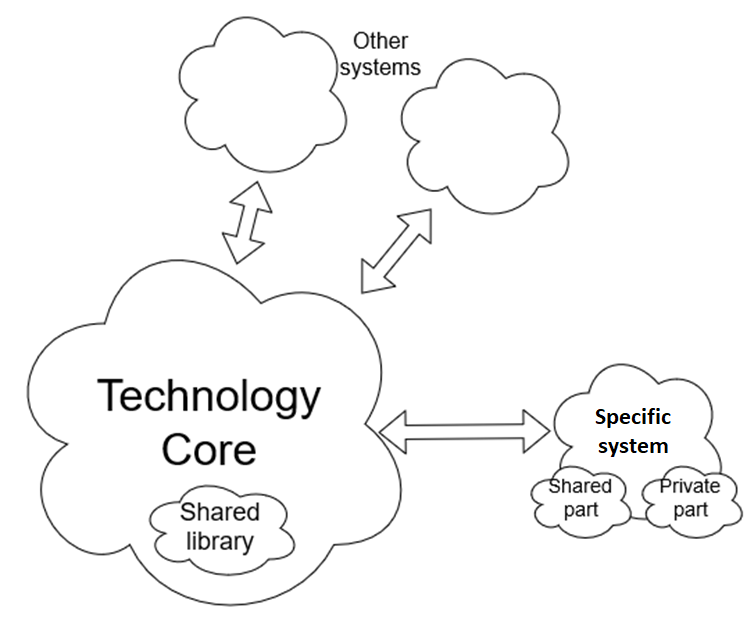
\includegraphics[width=0.6\textwidth]{figures/chapter0/ecosystem.png}}

\scnheader{Технология OSTIS}
\scnrelfromvector{текущие проекты}{Проект Экосистема OSTIS;Проект Метасистема IMS.ostis;Проект Семейство различных вариантов реализации универсального интерпретатора семантических моделей интеллектуальных систем\\
\scnaddlevel{1}
    \scnrelfromlist{подпроект}{Проект Программно реализованный на современных компьютерах универсальный интерпретатор семантических моделей интеллектуальных систем;Проект Семантический ассоциативный компьютер}
\scnaddlevel{-1}
;Проект Комплекс совместимых средств проектирования интеллектуальных систем\\
\scnaddlevel{1}
    \scnrelfromlist{подпроект}{Проект Встраиваемая типовая интеллектуальная система комплексной поддержки проектирования баз знаний;Проект Интеллектуальная система комплексной поддержки проектирования решателей задач интеллектуальных систем;Проект Интеллектуальная система комплексной поддержки проектирования вербальных интерфейсов интеллектуальных систем;Проект Интеллектуальная система комплексной поддержки проектирования невербальных интерфейсов}
\scnaddlevel{-1}
;Проект Семейство совместимых интеллектуальных справочных, обучающих и help-систем\\
\scnaddlevel{1}
    \scnrelfromlist{подпроект}{Проект Специализированные средства разработки совместимых интеллектуальных справочных, обучающих и help-систем различного назначения;Проект Комплекс семантически совместимых интеллектуальных справочных и обучающих систем по всем дисциплинам среднего образования;Проект Комплекс семантически совместимых интеллектуальных справочных и обучающих систем по всем дисциплинам, являющихся базовыми при подготовке инженеров по информационным специальностям;Проект Комплекс семантически совместимых интеллектуальных справочных и обучающих систем по всем специальным дисциплинам специальности ''Искусственный интеллект''{};Проект Семейство совместимых интеллектуальных справочных и обучающих систем по стандартам различного вида}
\scnaddlevel{-1}
;Проект Семейство совместимых интеллектуальных корпоративных систем ситуационного управления\\
\scnaddlevel{1}
    \scnrelfromlist{подпроект}{Проект Интеллектуальная корпоративная система ситуационного управления предприятием рецептурного производства;Проект Интеллектуальная корпоративная система ситуационного управления деятельностью выпускающей кафедры технического вуза}
\scnaddlevel{-1}
}
\scnrelfromvector{будущие проекты}{
Проект Семейство совместимых интеллектуальных систем автоматизации проектирования в различных областях;Проект Семейство совместимых порталов знаний\\
\scnaddlevel{1}
    \scnrelfrom{подпроект}{Проект Портал научных знаний по искусственному интеллекту}
\scnaddlevel{-1}
;Проект Семейство совместимых интеллектуальных систем экскурсионного обслуживания;Проект Семейство совместимых интеллектуальных геоинформационных систем;Проект Семейство совместимых интеллектуальных робототехнических систем и специализированных средств их разработки;Проект Семейство совместимых интеллектуальных систем персонального обслуживания и мониторинга\\
\scnaddlevel{1}
    \scnrelfromlist{подпроект}{Проект Интеллектуальная система персонального обслуживания и мониторинга пользователей и разработчиков компьютерных систем, входящих в Экосистему OSTIS;Проект Интеллектуальный персональный ассистент по взаимодействию с традиционными internet-системами и их пользователями;Проект Интеллектуальная система персонального комплексного медицинского мониторинга и контроля}
\scnaddlevel{-1}
}

\scnsegmentheader{Понятие технологии OSTIS}

\scnstartsubstruct

\scnheader{Технология OSTIS}
\scnidtf{Комплекс (семейство) технологий, обеспечивающих проектирование, производство, эксплуатацию и реинжиниринг интеллектуальных \textit{компьютерных систем (ostis-систем)}, предназначенных для автоматизации самых различных видов человеческой деятельности и в основе которых лежит смысловое представление и онтологическая систематизация знаний, а также агентно-ориентированная обработка знаний}
\scnidtf{Open Semantic Technology for Intelligent Systems}
\scnaddlevel{1}
\scntext{сокращение}{OSTIS}
\scnaddlevel{-1}
\scnidtf{Семейство (комплекс) \textit{ostis-технологий}}
\scnidtf{Комплексная открытая семантическая технология проектирования, производства, эксплуатации и реинжиниринга гибридных, семантически совместимых, активных и договороспособных \textit{интеллектуальных компьютерных систем}}
\scnheader{Технология OSTIS}
\scnrelfromset{принципы, лежащие в основе}{
\scnfileitem{Ориентация на разработку \textit{интеллектуальных компьютерных систем}, имеющих высокий уровень \textit{интеллекта} и, в частности, высокий уровень \textit{социализации}. Указанные системы, разработанные по \textit{Технологии OSTIS}, будем называть \textbf{ostis-системами}}
;\scnfileitem{Ориентация на \uline{комплексную} автоматизацию всех видов и областей \textit{человеческой деятельности} путем создания сети взаимодействующих и координирующих свою деятельность \textit{ostis-систем}. Указанную сеть \textit{ostis-систем} вместе с их пользователями будем называть \textbf{\textit{Экосистемой OSTIS}}}
;\scnfileitem{Поддержка перманентной эволюции \textit{ostis-систем} в ходе их эксплуатации.}
;\scnfileitem{\textit{Технология OSTIS} реализуется в виде сети \textit{ostis-систем}, которая является частью \textit{Экосистемы OSTIS}.
Ключевой \textit{ostis-системой} указанной сети является \textbf{Метасистема IMS.ostis} (Intelligent MetaSystem), реализующая \textbf{Ядро Технологии OSTIS}, которое включает в себя базовые (предметно независимые) методы и средства проектирования и производства \textit{ostis-систем} с интеграцией в их состав типовых встроенных подсистем поддержки эксплуатации и реинжиниринга \textit{ostis-систем}. Остальные \textit{ostis-системы}, входящие в состав рассматриваемой сети, реализуют различные специализированные \textit{ostis-технологии} проектирования различных классов \textit{ostis-систем}, обеспечивающих автоматизацию любых областей и \textit{видов человеческой деятельности}, кроме \textit{проектирования ostis-систем}.}
;\scnfileitem{Конвергенция и интеграция на основе смыслового представления знаний всевозможных научных направлений \textit{Искусственного интеллекта} (в частности, всевозможных базовых знаний и навыков решения интеллектуальных задач) в рамках \textit{Общей формальной семантической теории ostis-систем}.}
;\scnfileitem{Ориентация на разработку компьютеров нового поколения, обеспечивающих эффективную (в том числе, производительную) интерпретацию логико-семантических моделей \textit{ostis-систем}, представленных базами знаний этих систем и имеющих смысловое представление.}}

\scnsegmentheader{Понятие ostis-системы}

\scnstartsubstruct

\scnheader{ostis-система}
\scnidtf{\textit{интеллектуальная компьютерная система}, спроектированная и реализованная по требованиям и стандартам \textit{Технологии OSTIS}, которые задокументированы в \textit{Общей теории ostis-систем}}

\scnheader{ostis-система}
\scnidtf{интеллектуальная компьютерная система, построенная в соответствии с принципами и требованиями Технологии OSTIS}
\scnidtf{Множество ostis-систем различного назначения}
\scnaddlevel{1}
\scniselement{имя собственное}
\scnaddlevel{-1}
\scnidtf{Множество всевозможных интеллектуальных компьютерных систем, построенных по Технологии OSTIS}

\scnheader{ostis-система}
\scnsubset{интеллектуальная компьютерная система}
\scnidtf{\textit{интеллектуальная компьютерная система}, которая построена в соответствии с требованиями и стандартами \textit{Технологии OSTIS}, что обеспечивает существенное развитие целого ряда \textit{свойств} (способностей) этой \textit{компьютерной системы}, позволяющих значительно повысить \textit{уровень интеллекта} этой системы (и, прежде всего, ее \textit{уровень обучаемости} и \textit{уровень социализации})} 

\scnauthorcomment{Добавить классификацию из пояснения}

\scnsubdividing{индивидуальная ostis-система;коллективная ostis-система\\
\scnaddlevel{1}
    \scnsubdividing{простой коллектив ostis-систем;иерархический коллектив ostis-систем}   
\scnaddlevel{-1}
}

\scnheader{ostis-система}
\scnexplanation{интеллектуальная компьютерная система, разработанная, разрабатываемая или совершенствуемая по технологии OSTIS}
\scnnote{Когда речь идет о таком компоненте технологии OSTIS, как модели ostis-систем, фактически имеется в виду теория ostis-систем, включающая в себя строгое формальное уточнение того, как устроена ostis-система, какова ее архитектура, принципы организации памяти, принципы организации представления информации, принципы организации интерфейса с внешней средой (в том числе, с пользователями)}

\scnheader{ostis-система}
\scnrelfromset{принципы, лежащие в основе}{
\scnfileitem{Информация, хранимая в памяти \textit{ostis-системы}, имеет смысловое представление.}
;\scnfileitem{В основе организации решения задач в памяти \textit{ostis-системы} лежит \textit{агентно-ориентированная модель обработки информации}, управляемая ситуациями и событиями, возникающими в обрабатываемой информации (точнее, в обрабатываемой базе знаний).}
;\scnfileitem{Унификация базового набора (базовой системы) используемых понятий, что является основой обеспечения \textit{семантической совместимости} всех \textit{ostis-систем}.}
;\scnfileitem{В основе структуризации информации (базы знаний), хранимой в памяти \textit{ostis-системы}, лежит иерархическая система \textit{предметных областей} и соответствующих им \textit{формальных онтологий}.}
;\scnfileitem{Способность к пониманию (к семантическому погружению, к семантической интеграции) новых приобретаемых знаний (и, в том числе, новых навыков) в состав текущего состояния \textit{базы знаний}.}
;\scnfileitem{Способность к \textit{семантической конвергенции} (к обнаружению сходств) новых приобретаемых знаний (и, в частности, навыков) со знаниями, входящими в состав текущего состояния базы знаний \textit{ostis-системы}.}
;\scnfileitem{Способность \textit{ostis-системы} поддерживать высокий уровень своей \textit{семантической совместимости} (высокий уровень взаимопонимания) с другими \textit{ostis-системами}.}
;\scnfileitem{Способность ostis-системы согласовывать, координировать свою деятельность с другими \textit{ostis-системами}.}
;\scnfileitem{\scnauthorcomment{статья на OSTIS-2020}}
;\scnfileitem{\scnauthorcomment{статья на OSTIS-2020}}
;\scnfileitem{\scnauthorcomment{статья на OSTIS-2020}}
;\scnfileitem{\scnauthorcomment{статья на OSTIS-2020}}}
\scntext{следовательно}{Перечисленные свойства \textit{ostis-систем} свидетельствуют о том, что они имеют существенно более высокий \textit{уровень интеллекта} и, в частности, более высокий \textit{уровень социализации} по сравнению с современными \textit{интеллектуальными компьютерными системами}. \scnauthorcomment{См. начало Раздела 1.1}}

\scnheader{ostis-система}
\scnrelfromset{принципы, лежащие в основе}{
\scnfileitem{смысловое представление информации в памяти компьютерных систем, направленное на устранение недостатков современных компьютерных систем и технологий путем повышения уровня интеллектуальности компьютерных систем}
;\scnfileitem{децентрализация управления решателем задач
\begin{itemize}
	\item внутренняя МАС
	\item внешняя МАС
\end{itemize}}
;\scnfileitem{интеграция различных видов знаний}
;\scnfileitem{интеграция различных моделей решателей задач}
;\scnfileitem{ориентация на компьютеры нового поколения}
;\scnfileitem{обеспечение семантической совместимости компьютерных систем}
;\scnfileitem{обеспечение поддержания семантической совместимости компьютерных систем в ходе эволюции}
;\scnfileitem{способность к координации деятельности}}

\scnheader{ostis-система}
\scnrelfromset{принципы, лежащие в основе}{
\scnfileitem{Память ostis-системы является графодинамической (т.е. нелинейной (графовой) и структурно перестраиваемой). Переработка информации в памяти ostis-системы сводится не столько к изменению состояния элементов памяти (это происходит только при изменении синтаксического типа элементов и при изменении содержимого тех элементов, которые обозначают файлы), сколько к изменению \uline{конфигурации связей} между ними.}
;\scnfileitem{Хранение информации в памяти ostis-системы ориентируется на \uline{смысловое} представление информации – без синонимов, омонимов знаков и без семантической эквивалентности информационных конструкций.}
;\scnfileitem{С точки зрения архитектуры ostis-система представляет собой \uline{иерархическую} многоагентную систему с общедоступной памятью (т.е. с памятью, общедоступной \uline{всем} агентам ostis-системы). 
Заметим при этом, что общая память большинства исследуемых в настоящее время многоагентных систем является не общедоступной, а распределенной, т.е. представляет собой абстрактное (виртуальное) объединение, в состав которого входит память каждого агента многоагентной системы. Координация деятельности агентов ostis-системы при выполнении сложных \textit{действий в памяти} ostis-системы реализуется также через \textit{память ostis-системы} с помощью хранимых в памяти \textit{методов} решения различных классов задач, а также с помощью хранимых в памяти \textit{планов} решения конкретных задач.
На основании этого можно строить неограниченную иерархическую систему агентов ostis-системы – от элементарных агентов, обеспечивающих выполнение базовых действий в памяти ostis-системы, до неэлементарных агентов, представляющих собой коллективы (группы) элементарных и/или неэлементарных агентов, обеспечивающих решение различных типовых задач с помощью соответствующих методов и планов.}
;\scnfileitem{Организация выполнения \textit{ostis-системой действий во внешней среде} осуществляется следующим образом:
\begin{scnitemize}
	\item Выделяются классы \textit{элементарных действий во внешней среде}, для реализации каждого из которых вводятся \textit{эффекторные агенты} ostis-системы.
	\item Координация деятельности \textit{эффекторных агентов} ostis-системы при выполнении \textit{сложных действий во внешней среде} осуществляется через \textit{память ostis-системы} с помощью хранимых в памяти \textit{методов} и \textit{планов} решения различных задач во \textit{внешней среде}, а также с помощью \textit{рецепторных агентов} ostis-системы, обеспечивающих обратную связь и, соответственно, сенсомоторную координацию.
\end{scnitemize}}}

\scnheader{ostis-система}
\scnrelfromset{принципы, лежащие в основе}{
\scnfileitem{Способность понимать друг друга, а также любого своего пользователя
\scnaddlevel{-2}
\scnidtf {Совместимость используемых понятий (по терминам и по денотационной семантике)}
\scnidtf {Семантическая совместимость}
\scnaddlevel{2}}
;\scnfileitem{Способность поддерживать взаимопонимание в процессе индивидуальной эволюции, приводящей к расширению и/или корректировке системы используемых понятий}
;\scnfileitem{Способность координировать свою деятельность с другими системами при решении задач, которые усилиями одной (индивидуальной) интеллектуальной компьютерной системы не могут быть решены либо принципиально, либо за разумное время}}

\scnheader{ostis-система}
\scnrelfromset{принципы, лежащие в основе}{
\scnfileitem{Высокая степень индивидуальной обучаемости интеллектуальных компьютерных систем
\begin{itemize}
	\item гибкости
	\item стратифицированности
	\item рефлексивности
	\item универсальность средств представления и образования знаний
\end{itemize}}
;\scnfileitem{Высокая степень семантической совместимости и, как следствие, коллективной обучаемости интеллектуальных компьютерных систем
\begin{itemize}
	\item семантической совместимости
\end{itemize}}
;\scnfileitem{Основа для автоматизации рынка знаний}}

\scnmakeset{память*;ostis-система}
\scnrelfrom{сужение второго домена заданного отношения для заданного первого домена}{память ostis-системы}
\scnaddlevel{1}
\scnsubset{смысловая память}
\scnaddlevel{-1}


\scnmakeset{информация, хранимая в памяти кибернетической системы*;  ostis-система}
\scnrelfrom{сужение второго домена заданного отношения для заданного первого домена}{база знаний ostis-системы}
\scnaddlevel{1}
\scnsubset{смысловое представление информации}
\scnaddlevel{-1}


\scnheader{память ostis-системы}
\scnsubset{смысловая память}

\scnheader{информация, хранимая в памяти ostis-системы}
\scnsubset{смысловое представление информации}

\scnheader{решатель задач ostis-системы }
\scnsubset{агентно-ориентированная модель обработки информации в памяти}







































 

\scnendstruct

\end{SCn}

%\scsection[\scneditors{Никифоров С.А.;Бобёр  Е.С.}\protect\scnmonographychapter{Глава 2.6. Языковые средства формального описания синтаксиса и денотационной семантики различных языков в интеллектуальных компьютерных системах нового поколения}]{Предметная область и онтология информационных конструкций и языков}
\label{intro_lang}

\begin{SCn}

\scnsectionheader{\currentname}
\scnstartsubstruct

\scniselement{раздел базы знаний}
\scnrelfromlist{дочерний раздел}{\nameref{intro_sc_code};\nameref{intro_idtf};\nameref{intro_scg};\nameref{intro_scs};\nameref{intro_scn}}

\scntext{аннотация}{Поскольку предлагаемая Вашему вниманию \textit{Публикация Стандарта OSTIS-2021} представляет собой внешний текст основной части \textit{базы знаний} ostis-системы (\textit{Метасистемы IMS.ostis}), необходимо сразу во вводном разделе этого Стандарта пояснить основные принципы, лежащие в основе внутреннего представления \textit{баз знаний} в памяти \textit{ostis-систем}, а также некоторые правила и условные обозначения, используемые в оформлении внешних текстов \textit{баз знаний ostis-систем}.\\
Подчеркнем, что все эти принципы, правила и условные обозначения детально рассмотрены в соответствующих разделах \textit{Стандарта OSTIS}, но некоторые из них необходимо пояснить до начала ознакомления с основными положениями \textit{Технологии OSTIS}. Фактически речь идет о кратком руководстве конечных пользователей \textit{ostis-систем}.

Прежде, чем рассматривать \textit{внутренний язык*} и \textit{внешние языки*}, используемые \textit{ostis-системами}, необходимо уточнить понятие \textit{информационной конструкции}, понятие \textit{знака}, понятие \textit{текста}, понятие \textit{языка}.}\\

\scnheader{Предметная область информационных конструкций и языков}
\scniselement{предметная область}
\scnsdmainclasssingle{информационная конструкция}
\scnsdclass{дискретная информационная конструкция; элемент дискретной информационной конструкции; соответствие, заданное на множестве дискретных информационных конструкций; знак; знаковая конструкция;язык;семантически выделяемый класс дискретных информационных конструкций;язык ostis-системы;ограничитель;идентификатор;имя;предложение;sc.g-текст;sc.s-текст;sc.n-текст}

\scnhaselementlist{исследуемый класс классов первичных объектов исследования}{отношение, заданное на множестве элементов дискретных информационных конструкций\scnsupergroupsign ;параметр, заданный на множестве дискретных информационных конструкций\scnsupergroupsign ;отношение, заданное на множестве знаков\scnsupergroupsign ;отношение, заданное на множестве знаковых конструкций\scnsupergroupsign ;класс знаковых конструкций\scnsupergroupsign ;параметр, заданный на множестве знаковых конструкций\scnsupergroupsign ;отношение, заданное на множестве языков\scnsupergroupsign ;параметр, заданный на множестве языков\scnsupergroupsign}


\scnsdrelation{операционная семантика информационной конструкции*;алфавит*;ограничители*;разделители*;внешний идентификатор*;предложения*}


\scnheader{ostis-система}
\scnidtf{компьютерная система, построенная по Технологии OSTIS}

\scnheader{информационная конструкция}
\scnidtf{информация}
\scnidtf{конструкция (структура), содержащая некоторые сведения о некоторых сущностях}
\scnnote{Форма представления ("изображения"{}, "материализации"), форма структуризации (синтаксическая структура), а также \textit{смысл*} (денотационная семантика) \textit{информационных конструкций} могут быть самыми различными.}

\scnheader{дискретная информационная конструкция}
\scnsubset{информационная конструкция}
\scnexplanation{Каждая \textit{дискретная информационная конструкция} — это \textit{информационная конструкция}, смысл которой задается (1) множеством элементов (синтаксически атомарных фрагментов) этой информационной конструкции, (2) алфавитом этих элементов — семейством классов синтаксически эквивалентных элементов информационной конструкции, (3) принадлежностью каждого элемента информационной конструкции соответствующему классу синтаксически эквивалентных элементов информационной конструкции, (4) конфигурацией связей инцидентности между элементами информационной конструкции.}
    \scnaddlevel{1}
    \scntext{следствие}{Форма представления элементов дискретной информационной конструкции для анализа её смысла не требует уточнения. Главным является (1) наличие простой процедуры выделения (сегментации) элементов дискретной информационной конструкции (2) наличие простой процедуры установления синтаксической эквивалентности разных элементов дискретной информационной конструкции и (3) наличие простой процедуры установления принадлежности каждого элемента дискретной информационной конструкции соответствующему классу синтаксически эквивалентных элементов (т.е. соответствующему элементу алфавита).}
    \scnaddlevel{-1}

\scnheader{элемент дискретной информационной конструкции}
\scnidtf{синтаксически атомарный фрагмент (символ), входящий в состав дискретной информационной конструкции}
\scnnote{Поскольку дискретные информационные конструкции могут иметь общие элементы (атомарные фрагменты) и даже некоторые из них могут быть частями других информационных конструкций, элемент дискретной информационной конструкции может входить в состав сразу нескольких информационных конструкций.}
\scnrelto{второй домен}{элемент дискретной информационной конструкции*}

\scnheader{отношение, заданное на множестве элементов дискретных информационных конструкций\scnsupergroupsign}
\scnhaselement{элемент дискретной информационной конструкции*}
	\scnaddlevel{1}
	\scnidtf{быть элементарным (синтаксически атомарным) фрагментом заданной дискретной информационной конструкции*}
	\scnidtf{быть элементом (атомарным фрагментом) заданной дискретной информационной конструкции*}
	\scnidtf{Бинарное ориентированное отношение, каждая пара которого связывает (1) знак некоторой дискретной информационной конструкции и (2) знак одного из элементов этой дискретной информационной конструкции*}
	\scnrelfrom{второй домен}{элемент дискретной информационной конструкции}
	\scnaddlevel{-1}
\scnhaselement{синтаксическая эквивалентность элементов дискретных информационных конструкций*}
	\scnaddlevel{1}
	\scnidtf{быть синтаксически эквивалентными элементами (атомарными фрагментами) одной и той же или разных дискретных информационных конструкций, т.е. элементами, принадлежащими одному и тому же классу синтаксически эквивалентных элементов дискретных информационных конструкций*}
	\scnaddlevel{-1}
\scnhaselement{инцидентность элементов дискретных информационных конструкций*}
	\scnaddlevel{1}
	\scniselement{бинарное ориентированное отношение\scnsupergroupsign}
	\bigskip
	\scnnote{Для \textit{линейных информационных конструкций} -- это последовательность элементов (символов), входящих в состав этих конструкций.\\
	Для дискретных информационных конструкций, конфигурация которых имеет нелинейный характер, отношение инцидентности их элементов может быть разбито на несколько частных отношений инцидентности, каждое из которых является \uline{подмножеством} объединенного отношения инцидентности. Например, для двухмерных дискретных информационных конструкций это (1) инцидентность элементов информационных конструкций "по горизонтали"{} и (2) инцидентность элементов информационных конструкций "по вертикали".}
	\scnaddlevel{-1}

\scnhaselement{неэлементарный фрагмент дискретной информационной конструкции*}
	\scnaddlevel{1}
	\scnidtf{быть дискретной информационной конструкцией, которая является \uline{подструктурой} для заданной дискретной информационной конструкции, в состав которой входит (1) подмножество элементов заданной информационной конструкции и, соответственно, (2) подмножество пар инцидентности элементов заданной информационной конструкции.}
	\scnaddlevel{-1}
\scnhaselement{алфавит дискретной информационной конструкции*}
	\scnaddlevel{1}
	\scnidtf{быть семейством попарно непересекающихся \uline{классов} синтаксически эквивалентных элементов заданной дискретной информационной конструкции*}
	\scnaddlevel{-1}
\scnhaselement{первичная синтаксическая структура дискретной информационной конструкции*}
	\scnaddlevel{1}
	\scnidtf{быть \textit{графовой структурой}, которая полностью описывает конфигурацию заданной \textit{дискретной информационной конструкции} и которая включает в себя: (1) знаки всех тех классов синтаксически эквивалентных элементов, которым принадлежат элементы описываемой дискретной информационной конструкции, (2) знаки всех элементов (атомарных фрагментов) описываемой информационной конструкции, (3) пары, описывающие инцидентность элементов описываемой информационной конструкции, (4) пары, описывающие принадлежность элементов описываемой информационной конструкции соответствующим классам синтаксически эквивалентных элементов этой информационной конструкции.}
	\scnaddlevel{-1}
\scnhaselement{синтаксическая эквивалентность дискретных информационных конструкций*}
	\scnaddlevel{1}
	\scndefinition{Дискретные информационные конструкции $\bm{Ti}$ и $\bm{Tj}$ являются синтаксически эквивалентными в том и только в том случае, если между конструкцией $\bm{Ti}$ и конструкцией $\bm{Tj}$ существует \uline{изоморфизм}, в рамках которого каждому элементу конструкции $\bm{Ti}$ соответствует синтаксически эквивалентный элемент конструкции $\bm{Tj}$, т.е. элемент, принадлежащий тому же классу синтаксически эквивалентных элементов дискретных информационных конструкций. И наоборот.}
	\scnaddlevel{-1}
\scnhaselement{копия дискретной информационной конструкции*}
	\scnaddlevel{1}
	\scnsubset{синтаксическая эквивалентность дискретных информационных конструкций*}
	\scnidtfdef{быть дискретной информационной конструкцией, которая не только синтаксически эквивалентна заданной, но и содержит информацию о форме представления элементов копируемой информационной конструкции*}
	\scnaddlevel{-1}
\scnhaselement{семантическая эквивалентность дискретных информационных конструкций*}
	\scnaddlevel{1}
	\scndefinition{Информационная конструкция $\bm{Ti}$ и информационная конструкция $\bm{Tj}$ являются \uline{семантически эквивалентными} в том и только в том случае, если \uline{каждая} сущность (в том числе, и каждая связь между сущностями), описываемая в информационной конструкции $\bm{Ti}$ описывается также и в информационной конструкции $\bm{Tj}$. И наоборот.}
	\scnaddlevel{-1}
\scnhaselement{семантическое расширение дискретной информационной конструкции*}
	\scnaddlevel{1}
	\scndefinition{Информационная конструкция $\bm{Tj}$ является семантическим расширением информационной конструкции $\bm{Ti}$ в том и только в том случае, если \uline{каждая} сущность, описываемая в $\bm{Ti}$, описывается также и в $\bm{Tj}$, но обратное неверно.}
	\scnaddlevel{-1}
\scnhaselement{синтаксис информационной конструкции*}
	\scnaddlevel{1}
	\scnidtf{синтаксическая структура информационной конструкции*}
	\scnidtf{быть синтаксической структурой для заданной информационной конструкции*}
	\scnidtf{Бинарное ориентированное отношение, каждая пара которого связывает знак некоторой информационной конструкции с синтаксической структурой этой конструкции*}
	\scnidtf{описание того, из каких частей состоит заданная информационная конструкция и как эти части (фрагменты) связаны между собой*}
	\scnrelfrom{первый домен}{информационная конструкция}
	\scnaddlevel{-1}
\bigskip
\scnhaselement{смысл*}
	\scnaddlevel{1}
	\scnidtf{смысл информационной конструкции*}
	\scnidtf{денотационная семантика информационной конструкции*}
	\scnidtf{семантическая (смысловая) структура информационной конструкции*}
	\scnidtf{быть семантической (смысловой) структурой для заданной информационной конструкции*}
	\scnidtf{быть смыслом заданной информационной конструкции*}
	\scnidtf{быть явным (формальным) представлением того, какие сущности описывает данная информационная конструкция и как эти сущности связаны между собой*}
	\scnidtf{Бинарное ориентированное отношение, каждая пара которого связывает некоторую информационную конструкцию с ее смыслом (смысловой структурой)*}
	\scnaddlevel{-1}
\scnhaselement{операционная семантика информационной конструкции*}
	\scnaddlevel{1}
	\scnidtf{правила трансформации заданной информационной конструкции*}
	\scnidtf{описание того, на основании каких правил можно осуществлять действия по преобразования (обработке, трансформации) заданной информационной конструкции, оставляя ее в рамках класса синтаксически и семантически правильных информационных конструкций*}
	\scnidtf{Бинарное ориентированное отношение, каждая пара которого связывает знак некоторой информационной конструкции со множеством правил ее трансформации*}
    \scnaddlevel{-1}
	
\scnheader{операционная семантика информационной конструкции*}
\scnrelfrom{второй домен}{операционная семантика информационной конструкции}
	
\scnheader{соответствие, заданное на множестве дискретных информационных конструкций}
\scnhaselement{соответствие между синтаксической структурой информационной конструкции и смыслом этой конструкции*}
\scnaddlevel{1}
	\scnidtf{Множество ориентированных пар, первым компонентом которых является ориентированная пара, состоящая из (1) знака синтаксической структуры некоторой информационной конструкции и (2) знака смысловой структуры этой конструкции, а вторым компонентом которых является множество ориентированных пар, связывающих фрагменты синтаксической структуры заданной информационной конструкции (которые описывают либо структуру фрагментов заданной конструкции, либо связи между фрагментами этой конструкции) с теми фрагментами смысловой структуры заданной информационной конструкции, которые семантически эквивалентны либо синтаксически представленным фрагментам заданной информационной конструкции, либо синтаксически представленным связям между такими фрагментами*}
	\scnsubset{соответствие*}
\scnaddlevel{-1}

\scnheader{параметр, заданный на множестве дискретных информационных конструкций\scnsupergroupsign}
\scnhaselement{размерность дискретных информационных конструкций\scnsupergroupsign}
	\scnaddlevel{1}
	\scnidtf{типология дискретных информационных конструкций, определяемая их размерностью}
	\scnexplanation{Это параметр дискретных информационных конструкций, определяющий характер \uline{инцидентности} элементов таких конструкций.}
	\scnhaselement{линейная информационная конструкция}
		\scnaddlevel{1}
		\scnidtfexp{дискретная информационная конструкция, каждый элемент которой может иметь не более двух инцидентных ему элементов (один слева, другой справа)}
		\scnaddlevel{-1}
	\scnhaselement{двухмерная информационная конструкция}
		\scnaddlevel{1}
		\scnidtfexp{дискретная информационная конструкция, каждый элемент которой может иметь не более четырех инцидентных ему элементов (слева-справа, сверху-снизу)}
		\scnaddlevel{-1}
	\scnhaselement{трехмерная информационная конструкция}
		\scnaddlevel{1}
		\scnidtfexp{дискретная информационная конструкция, каждый элемент которой может иметь не более шести инцидентных ему элементов (слева-справа, сверху-снизу, сзади-спереди)}
		\scnaddlevel{-1}
	\scnhaselement{четырехмерная информационная конструкция}
		\scnaddlevel{1}
		\scnidtfexp{дискретная информационная конструкция, каждый элемент которой может иметь не более восьми инцидентных ему элементов (например, слева-справа, сверху-снизу, сзади-спереди, раньше-позже)}
		\scnaddlevel{-1}
	\scnhaselement{графовая информационная конструкция}
		\scnaddlevel{1}
		\scnidtfexp{дискретная информационная конструкция, множество элементов которой разбивается на два подмножества — связки и узлы. При этом узлы могут иметь \uline{неограниченное} количество инцидентных им связок}
			\scnaddlevel{1}
			\scnnote{А в некоторых графовых информационных конструкциях и связки могут иметь неограниченное количество инцидентных им других связок}
			\scnaddlevel{-1}
		\scnaddlevel{-1}
	\scnaddlevel{-1}
\scnhaselement{типология дискретных информационных конструкций, определяемая их носителем\scnsupergroupsign}
    \scnaddlevel{1}
        \scnhaselement{некомпьютерная форма представления дискретных информационных конструкций}
	    \scnaddlevel{1}
	    \scnsuperset{аудио-сообщение}
    		\scnaddlevel{1}
		    \scnidtf{речевое сообщение}
		    \scnidtf{информационная конструкция, представленная в звуковой форме}
		    \scnaddlevel{-1}
	    \scnsuperset{информационная конструкция, представленная на языке жестов}
	    \scnsuperset{информационная конструкция, представленная в письменной форме}
    		\scnaddlevel{1}
		    \scnnote{Конкретный вид носителя для письменной формы представления информации может быть разным — бумага, папирус, береста, камень...}
		    \scnaddlevel{-1}
	\scnaddlevel{-1}
	\scnhaselement{файл}
		\scnaddlevel{1}
		\scnidtf{компьютерная ("электронная") форма (формат) представления и хранения информационных конструкций}
		\scnnote{Представление информационных конструкций в виде файлов ориентировано на представление \uline{дискретных} (!) информационных конструкций. Поэтому "файловое"{} представление недискретных информационных конструкций (например, различного рода сигналов) предполагает "дискретизацию"{} таких конструкций, т.е. преобразование их в дискретные. Так преобразуются аудио-сигналы (в частности, речевые сообщения), изображения, видео-сигналы и др.}
		\scnaddlevel{-1}
	\scnaddlevel{-1}
\scnhaselement{уровень унификации представления синтаксически эквивалентных элементов дискретных информационных конструкций\scnsupergroupsign}
	\scnaddlevel{1}
	\scnidtf{уровень "членораздельности"{} дискретных информационных конструкций}
	\scnnote{Чем выше уровень унификации представления элементов дискретных информационных конструкций, тем проще реализуется (1) процедура выделения (сегментации) элементов дискретной информационной конструкции, (2) процедура установления синтаксической эквивалентности этих элементов и (3) процедура их распознавания, т.е. процедура установления их принадлежности соответствующим классам синтаксически эквивалентных элементов.}
	\scnhaselement{дискретная информационная конструкция с низким уровнем унификации представления элементов}
		\scnaddlevel{1}
		\scnsuperset{аудио-сообщение}
		\scnsuperset{информационная конструкция, представленная на языке жестов}
		\scnsuperset{рукопись или её копия}
		\scnaddlevel{-1}
	\scnhaselement{дискретная информационная конструкция с высоким уровнем унификации представления элементов}
		\scnaddlevel{1}
		\scnsuperset{печатный текст}
		\scnsuperset{файл}
		\scnaddlevel{-1}
	\scnaddlevel{-1}
\scnaddlevel{-1}	

\scnheader{знак}
\scnexplanation{фрагмент информационной конструкции, который условно представляет (изображает) некоторую описываемую сущность, которую называют денотатом знака}
\scnsubdividing{знак, являющийся элементом дискретной информационной конструкции;знак, являющийся неатомарным фрагментом дискретной информационной конструкции}
\scnnote{Отсутствие знака, обозначающего некоторую сущность, не означает отсутствие самой этой сущности. Это означает только то, что мы даже не догадываемся о её существовании и, следовательно, не приступили к её исследованию.}

\newpage
\scnheader{отношение, заданное на множестве знаков\scnsupergroupsign}
\scnnote{Поскольку все знаки являются дискретными информационными конструкциями, множество знаков является областью задания всех отношений, заданных на множестве дискретных информационных конструкций. Тем не менее есть как минимум одно отношение, специфичное для множества знаков.}
\scnhaselement{синонимия знаков*}
	\scnaddlevel{1}
	\scndefinition{Знаки являются синонимичными в том и только в том случае, если они обозначают одну и ту же сущность.}
	\scnnote{Синонимичные знаки могут быть синтаксически эквивалентными, а могут и не быть таковыми.}
	\scnaddlevel{-1}

\scnheader{знаковая конструкция}
\scnsubset{дискретная информационная конструкция}
\scnidtfexp{дискретная информационная конструкция, которая в общем случае представляет собой конфигурацию знаков и специальных фрагментов информационной конструкции, обеспечивающих структуризацию конфигурации знаков — различного вида разделителей и ограничителей}
	\scnaddlevel{1}
	\scnnote{Для некоторых знаковых конструкций и даже для некоторых языков необходимость в разделителях и ограничителях может отсутствовать.}
	\scnaddlevel{-1}	
	
\scnheader{отношение, заданное на множестве знаковых конструкций\scnsupergroupsign}
\scnhaselement{знак*}
	\scnaddlevel{1}
	\scnidtf{быть знаком для заданной знаковой конструкции*}
	\scnaddlevel{-1}
\scnhaselement{разделитель знаковой конструкции*}
\scnhaselement{разделители знаковой конструкции*}
	\scnaddlevel{1}
	\scnidtf{Множество всех разделителей, входящих в состав заданной знаковой конструкции*}
	\scnaddlevel{-1}
\scnhaselement{ограничитель знаковой конструкции*}
\scnhaselement{ограничители знаковой конструкции*}
\scnhaselement{семантическая смежность знаковых конструкций*}
	\scnaddlevel{1}
	\scndefinition{Знаковые конструкции $\bm{Ti}$ и $\bm{Tj}$ являются смежными в том и только в том случае, если существуют синонимичные знаки $\bm{Ti}$ и $\bm{Tj}$, один из которых входит в состав конструкции $\bm{Ti}$, а второй — в состав конструкции $\bm{Tj}$}
	\scnaddlevel{-1}
\scnhaselement{конкатенация знаковых конструкций*}
	\scnaddlevel{1}
	\scnidtf{декомпозиция заданной знаковой конструкции на последовательность знаковых конструкций*}
	\scnaddlevel{-1}
	
\scnheader{класс знаковых конструкций\scnsupergroupsign}
\scnhaselement{семантически элементарная знаковая конструкция}
	\scnaddlevel{1}
	\scnidtf{знаковая конструкция, описывающая некоторую (одну) связь между некоторыми сущностями}
	\scnaddlevel{-1}
\scnhaselement{семантически связная знаковая конструкция}
	\scnaddlevel{1}
	\scnidtfdef{знаковая конструкция, которую можно представить в виде конкатенации семантически элементарных знаковых конструкций, каждая из которых семантически смежна предшествующей и последующей семантически элементарной знаковой конструкции}
	\scnaddlevel{-1}

\scnheader{параметр, заданный на множестве знаковых конструкций\scnsupergroupsign}
\scnhaselement{семантическая связность знаковых конструкций\scnsupergroupsign}
	\scnaddlevel{1}
	\scnhaselement{семантически связная знаковая конструкция}
	\scnhaselement{семантически несвязная знаковая конструкция}
	    \scnaddlevel{1}
    	\scnhaselementrole{пример}{\scnfilelong{В огороде бузина, а в Киеве дядька}}
    	\scnaddlevel{-1}
	\scnaddlevel{-1}
\scnhaselement{наличие разделителей и ограничителей\scnsupergroupsign}
	\scnaddlevel{1}
	\scnhaselement{знаковая конструкция, содержащая разделители и-или ограничители}
	\scnhaselement{знаковая конструкция без разделителей и ограничителей}

\newpage
\scnheader{язык}
\scnidtfexp{класс знаковых конструкций, для которого существуют (1) общие правила их построения и (2) общие правила их соотнесения с теми сущностями и конфигурациями сущностей, которые описываются (отражаются) указанными знаковыми конструкциями}
\scnidtf{класс знаковых конструкций, эквивалентных с точки зрения правил их построения и правил их семантической интерпретации}
\scnsubdividing{язык, у которого все знаки, входящие в состав его знаковых конструкций, являются элементарными фрагментами этих конструкций\\
	\scnaddlevel{1}
	\scnnote{Для языков такого типа существенно упрощаются методы обработки их текстов.}
	\scnaddlevel{-1}
;язык, у которого знаки, входящие в состав его знаковых конструкций, в общем случае не являются элементарными фрагментами этих конструкций}
\scnsubdividing{язык, знаковые конструкции которого содержат разделители и ограничители;язык, знаковые конструкции которого не содержат разделителей и ограничителей\\
	\scnaddlevel{1}
	\scntext{следствие}{Знаковые конструкции такого языка состоят \uline{только} из знаков.}
	\scnaddlevel{-1}}

\scnheader{отношение, заданное на множестве языков\scnsupergroupsign}
\scnidtf{отношение, область определения которого включает в себя множество всевозможных языков}
\scnhaselement{текст заданного языка*}
	\scnaddlevel{1}
	\scnidtf{знаковая конструкция, принадлежащая заданному языку*}
	\scnidtf{синтаксически правильная (правильно построенная) знаковая конструкция заданного языка*}
	\scnidtf{синтаксически корректная и целостная знаковая конструкция для заданного языка*}
	\scneq{{\normalfont(}синтаксически корректная знаковая конструкция для заданного языка* $\cap$ синтаксически целостная знаковая конструкция для заданного языка*{\normalfont)}}
	\scnaddlevel{-1}
\scnhaselement{синтаксически корректная знаковая конструкция для заданного языка*}
	\scnaddlevel{1}
	\scnidtf{знаковая конструкция, не содержащая синтаксических ошибок для заданного языка}
	\scnaddlevel{-1}
\scnhaselement{синтаксически целостная знаковая конструкция для заданного языка*}
\scnhaselement{синтаксически неправильная знаковая конструкция для заданного языка*}
	\scnaddlevel{1}
	\scneq{{\normalfont(}синтаксически некорректная знаковая конструкция для заданного языка* $\cup$ синтаксически нецелостная знаковая конструкция для заданного языка*{\normalfont)}}
	\scnsuperset{синтаксически некорректная знаковая конструкция для заданного языка*}
	\scnsuperset{синтаксически нецелостная знаковая конструкция для заданного языка*}
	\scnaddlevel{-1}
\scnhaselement{знание, представленное на заданном языке*}
	\scnaddlevel{1}
	\scnidtf{семантически правильный текст заданного языка*}
	\scneq{(семантически корректный текст заданного языка* $\cap$ семантически целостный текст заданного языка*)}
	\scnidtf{истинный текст заданного языка*}
	\scnidtf{истинное высказывание, представленное на заданном языке*}
	\scnaddlevel{-1}
\scnhaselement{семантически корректный текст заданного языка*}
	\scnaddlevel{1}
	\scnidtf{текст заданного языка, не содержащий семантических ошибок, противоречащих признанным закономерностям и фактам*}
	\scnaddlevel{-1}
\scnhaselement{семантически целостный текст заданного языка*}
	\scnaddlevel{1}
	\scnidtf{текст заданного языка, содержащий достаточную информацию для установления его истинности*}
	\scnaddlevel{-1}
\scnhaselement{семантически неправильный текст для заданного языка*}
	\scnaddlevel{1}
	\scneq{(семантически некорректный текст для заданного языка* $\cup$ семантически нецелостный текст для заданного языка*)}
	\scnsuperset{семантически некорректный текст для заданного языка*}
	\scnsuperset{семантически нецелостный текст для заданного языка*}
	\scnaddlevel{-1}
\scnhaselement{алфавит*}
	\scnaddlevel{1}
	\scnidtf{алфавит заданной информационной конструкции или заданного языка*}
	\scnidtf{семейство классов, синтаксически эквивалентных элементов (элементарных фрагментов) заданной информационной конструкции или информационных конструкций заданного языка*}
	\scnaddlevel{-1}
\scnhaselement{семейство классов синтаксически эквивалентных разделителей*}
	\scnaddlevel{1}
	\scnidtf{семейство классов синтаксически эквивалентных разделителей, входящих в состав заданной информационной конструкции или в состав информационных конструкций заданного языка*}
	\scnaddlevel{-1}
\scnhaselement{семейство классов синтаксически эквивалентных ограничителей*}
	\scnaddlevel{1}
	\scnidtf{семейство классов синтаксически эквивалентных ограничителей, входящих в состав заданной информационной конструкции или в состав информационных конструкций заданного языка*}
	\scnaddlevel{-1}	
\scnhaselement{синтаксис языка*}
	\scnaddlevel{1}
	\scnidtf{быть теорией правильно построенных информационных конструкций, принадлежащих заданному языку*}
	\scnidtf{определение понятия правильно построенной информационной конструкции заданного языка*}
	\scnidtf{синтаксические правила заданного языка*}
	\scnidtf{быть синтаксическими правилами заданного языка *}
	\scnidtf{Бинарное ориентированное отношение, каждая пара которого связывает знак некоторого языка с описанием синтаксически выделяемых классов фрагментов конструкций заданного языка, с описанием отношений, заданных на этих классах и с конъюнкцией кванторных высказываний, являющихся синтаксическими правилами заданного языка, то есть правилами, которым должны удовлетворять все синтаксические правильные (правильно построенные) конструкции (тексты) указанного языка*}
	\scnnote{При представлении синтаксиса (синтаксических правил) заданного языка используются все те понятия, которые вводятся для представления синтаксических структур информационных конструкций, принадлежащих указанному языку. Это и синтаксически выделяемые классы фрагментов указанных информационных конструкций, и отношения, заданные на множестве таких фрагментов.}
	\scnrelfrom{второй домен}{синтаксис языка}
	\scnaddlevel{-1}
\scnhaselement{описание синтаксических понятий языка*}
    \scnaddlevel{1}
    \scnidtf{описание синтаксически выделяемых классов фрагментов конструкций заданного языка*}
    \scnrelfrom{второй домен}{описание синтаксических понятий языка}
    \scnaddlevel{1}
        \scnrelto{обобщенное включение}{синтаксис языка}
    \scnaddlevel{-2}
\scnhaselement{синтаксические правила языка*}
    \scnaddlevel{1}
    \scnidtf{синтаксические правила заданного языка*}
    \scnrelfrom{второй домен}{синтаксические правила языка}
    \scnaddlevel{-1}
\scnhaselement{денотационная семантика языка*}
	\scnaddlevel{1}
	\scnidtf{быть теорией морфизмов, связывающих правильно построенные информационные конструкции заданного языка с описываемыми конфигурациями описываемых сущностей*}
	\scnaddlevel{-1}

\scnhaselement{денотационная семантика языка*}
	\scnaddlevel{1}
	\scnidtf{семантические правила заданного языка*}
	\scnidtf{быть семантическими правилами заданного языка *}
	\scnidtf{Бинарное ориентированное отношение, каждая пара которого связывает знак некоторого языка с описанием основных семантических понятий заданного языка и конъюнкцией кванторных высказываний, являющихся семантическими правилами заданного языка, то есть правилами, которым должны удовлетворять семантически правильные \uline{смысловые} информационные конструкции, соответствующие (семантические эквивалентные) синтаксически правильным конструкциям (текстам) заданного языка*}
	\scnnote{При формулировке семантических правил заданного языка используются понятия, введенные в рамках базовых онтологий (онтологий самого высокого уровня, в которых рассматриваются самые общие классы описываемых сущностей, самые общие отношения и параметры).}
	\scnrelfrom{второй домен}{денотационная семантика языка}
	\scnaddlevel{-1}
\scnhaselement{описание семантических понятий языка*}
	\scnaddlevel{1}
	\scnrelfrom{второй домен}{описание семантических понятий языка}
	\scnaddlevel{-1}
\scnhaselement{семантические правила языка*}
	\scnaddlevel{1}
	\scnrelfrom{второй домен}{семантические правила языка}
	\scnaddlevel{-1}
\bigskip
\scnhaselement{семантическая эквивалентность языков*}
	\scnaddlevel{1}
	\scnidtf{быть семантически эквивалентными языками*}
	\scndefinition{Язык $\bm{Li}$ и язык $\bm{Lj}$ будем считать \textit{семантически эквивалентными языками*} в том и только в том случае, если для каждого текста, принадлежащего языку $\bm{Li}$, существует \textit{семантически эквивалентный текст*}, принадлежащий языку $\bm{Lj}$, и наоборот.}
	\scnaddlevel{-1}
\scnhaselement{семантическое расширение языка*}
	\scnaddlevel{1}
	\scnrelboth{обратное отношение}{семантическое сужение языка*}
	\scndefinition{Язык $\bm{Lj}$ будем считать \textit{семантическим расширением*} языка $\bm{Li}$ в том и только в том случае, есть ли для каждого текста, принадлежащего языку $\bm{Li}$, существует \textit{семантически эквивалентный текст*}, принадлежащий языку $\bm{Lj}$, но обратное неверно.}
	\scnaddlevel{-1}
\scnhaselement{синтаксическое расширение языка*}
	\scnaddlevel{1}
	\scnidtf{быть семантически эквивалентным надмножеством заданного языка*}
	\scndefinition{Язык $\bm{Lj}$ будем считать \textit{синтаксическим расширением*} языка $\bm{Li}$ в том и только в том случае, если:
    \begin{scnitemize}
    \item $\bm{L_j} \supset \bm{Li}$ (то есть все тексты языка $\bm{Li}$ являются также и текстами языка $\bm{Lj}$, но обратное неверно);
    \item Язык $\bm{Lj}$ и язык $\bm{Li}$ являются \textit{семантически эквивалентными языками*}.
    \end{scnitemize}
    }
	\scnaddlevel{-1}
\scnhaselement{синтаксическое ядро языка*}
	\scnaddlevel{1}
	\scnidtf{быть синтаксическим ядром заданного языка*}
	\scnidtf{быть семантически эквивалентным подмножеством заданного языка, имеющим минимальную синтаксическую сложность*}
	\scnaddlevel{-1}
\scnhaselement{направление синтаксического расширения ядра заданного языка*}
	\scnaddlevel{1}
	\scnidtf{быть правилом трансформации информационных конструкций, принадлежащих заданному языку, которое описывает одно из направлений перехода от множества конструкций ядра этого языка ко множеству всех принадлежащих ему информационных конструкций*}
	\scnaddlevel{-1}
\scnhaselement{операционная семантика языка*}
	\scnaddlevel{1}
	\scnidtf{Бинарное ориентированное отношение, каждая пара которого связывает знак некоторого языка со множеством правил трансформации текстов этого языка*}
	\scnrelfrom{второй домен}{операционная семантика языка}
	\scnaddlevel{-1}
\scnhaselement{внутренний язык*}
	\scnaddlevel{1}
	\scnidtf{быть внутренним языком для заданной системы, основанной на обработке информации, или заданного множества таких систем*}
	\scnidtf{быть языком внутреннего представления информации в памяти заданной системы, основанной на обработке информации или заданного класса таких систем*}
	\scnaddlevel{-1}
\scnhaselement{внешний язык*}
	\scnaddlevel{1}
	\scnidtf{быть внешним языком для заданной системы, основанной на обработке информации, или заданного множества таких систем*}
	\scnidtf{быть языком, используемым для обмена информацией заданной системы, основанной на обработке информации, или заданного множества таких систем с другими системами, основанными на обработке информации, (в том числе, и с себе подобными)*}
	\scnaddlevel{-1}
\scnhaselement{используемый язык*}
	\scnaddlevel{1}
	\scneq{{\normalfont(}внутренний язык* $\cup$ внешний язык*{\normalfont)}}
	\scnidtf{язык, используемый заданной системой, основанной на обработке информации или заданного множества таких систем*}
	\scnidtf{язык, носителем которого является (которым владеет) данная система, основанная на обработке информации}
	\scnaddlevel{-1}
\scnhaselement{используемые языки*}

\scnheader{параметр, заданный на множестве языков\scnsupergroupsign}
\scnidtf{признак классификации языков}
\scnidtf{свойство, которым обладают языки}
\scnidtf{свойство языков, на основании которого можно осуществлять их классификацию}
\scnidtf{семейство классов эквивалентности языков, трактуемой в контексте того или иного свойства (характеристики), присущего языкам}
\scnhaselement{семантическая мощность языка\scnsupergroupsign}
	\scnaddlevel{1}
	\scnidtf{класс языков, семантически эквивалентных друг другу}
	\scnhaselement{универсальный язык}
		\scnaddlevel{1}
		\scnidtf{класс всевозможных универсальных языков}
		\scnnote{Очевидно, что все универсальные языки (если они действительно таковыми являются, а не только претендуют на это) семантически эквивалентны друг другу, т.е. имеют одинаковую семантическую мощность.}
		\scnaddlevel{-1}
	\scnaddlevel{-1}
\scnhaselement{уровень синтаксической сложности представления знаков в текстах языка\scnsupergroupsign}
	\scnaddlevel{1}
	\scnhaselement{язык, в текстах которого все знаки представлены синтаксически элементарными фрагментами}
	\scnhaselement{язык, в текстах которого знаки в общем случае представлены синтаксически неэлементарными фрагментами}
	\scnaddlevel{-1}
\scnhaselement{использование разделителей и ограничителей в текстах языка\scnsupergroupsign}
	\scnaddlevel{1}
	\scnhaselement{язык, в текстах которого не используются разделители и ограничители}
	\scnhaselement{язык, в текстах которого используются разделители и ограничители}
	\scnaddlevel{-1}
\scnhaselement{уровень сложности процедуры установления синонимии знаков в текстах языка\scnsupergroupsign}
	\scnaddlevel{1}
	\scnhaselement{язык, в рамках каждого текста которого синонимичные знаки отсутствуют}
		\scnaddlevel{1}
		\scnexplanation{В текстах такого языка знак каждой описываемой сущности входит \uline{однократно}.}
		\scnaddlevel{-1}
	\scnhaselement{язык, в рамках которого синонимичные знаки представлены синтаксически эквивалентными фрагментами текстов}
	\scnhaselement{флективный язык}
		\scnaddlevel{1}
		\scnidtf{язык, в рамках которого синонимичные знаки могут быть представлены синтаксически неэквивалентными фрагментами, но фрагментами, являющимися модификациями некоторого "ядра"{} этих фрагментов (при склонении и спряжении этих знаков).}
		\scnaddlevel{-1}
	\scnhaselement{язык, в рамках которого синонимичные знаки в общем случае могут быть представлены синтаксически неэквивалентными текстовыми фрагментами, структура которых носит непредсказуемый характер}
	\scnaddlevel{-1}
\scnhaselement{наличие омонимии в текстах языка\scnsupergroupsign}
	\scnaddlevel{1}
	\scnhaselement{язык, в текстах которого присутствует омонимия знаков}
		\scnaddlevel{1}
		\scnidtf{язык, в текстах которого присутствуют синтаксически эквивалентные, не синонимичные знаки}
		\scnaddlevel{-1}
	\scnhaselement{язык, в текстах которого омонимия знаков отсутствует}
	\scnaddlevel{-1}

\scnheader{семантически выделяемый класс дискретных информационных конструкций}
\scnhaselement{синтаксическая структура информационной конструкции}
    \scnaddlevel{1}
    \scnrelto{второй домен}{синтаксис информационной конструкции*}
    \scnsuperset{первичная синтаксическая структура информационной конструкции}
    \scnsuperset{вторичная синтаксическая структура информационной конструкции}
    \scnaddlevel{-1}
\scnhaselement{синтаксис языка}
\scnhaselement{описание синтаксических понятий языка}
\scnhaselement{синтаксические правила языка}
\scnhaselement{денотационная семантика языка}
\scnhaselement{описание семантических понятий языка}
\scnhaselement{семантические правила языка}
\scnhaselement{операционная семантика языка}
\scnhaselement{смысл}
    \scnaddlevel{1}
    \scnrelto{второй домен}{смысл*}
    \scnidtf{смысловая информационная конструкция}
    \scnidtf{смысловое представление информационной конструкции}
    \scnidtf{явное (формальное) представление описываемых сущностей и связей между ними}
    \scnidtf{смысловое представление информации}
    \scnnote{Для явного представления описываемых сущностей и связей между ними требуется существенное упрощение синтаксической структуры информационных конструкций}
    \scnaddlevel{-1}
    
\scnheader{язык ostis-системы}
\scnidtf{язык, используемый ostis-системами}
\scnidtf{язык представления информационных конструкций в ostis-системах}
\scnidtf{Множество языков, которыми "владеют"\ ostis-системы}
\scnsubset{формальный язык}
\scnsubset{универсальный язык}
\scnrelto{используемые языки}{ostis-система}

\scnhaselement{SC-код}
\scnaddlevel{1}
\scnidtf{Semantic Computer Code}
\scnrelto{внутренний язык}{ostis-система}
\scniselement{универсальный язык}
\scnaddlevel{-1}

\scnhaselement{SCg-код}
\scnaddlevel{1}
\scnidtf{Semantic Code graphical}
\scnidtf{\textit{внешний язык*} ostis-систем, тексты которого представляют собой графовые структуры общего вида с точно заданной \textit{денотационной семантикой*}}
\scnrelto{внешний язык}{ostis-система}
\scniselement{универсальный язык}
\scnaddlevel{-1}

\scnhaselement{SCs-код}
\scnaddlevel{1}
\scnidtf{Semantic Code string}
\scnidtf{\textit{внешний язык*} ostis-систем, тексты которого представляют собой строки (цепочки) символов}
\scnrelto{внешний язык}{ostis-система}
\scniselement{универсальный язык}
\scnaddlevel{-1}

\scnhaselement{SCn-код}
\scnaddlevel{1}
\scnidtf{Semantic Code natural}
\scnidtf{\textit{внешний язык*} ostis-систем, тексты которого представляют собой двухмерные матрицы символов, являющиеся результатом форматирования, двухмерной структуризации текстов SCs-кода.}
\scnrelto{внешний язык}{ostis-система}
\scniselement{универсальный язык}
\scnaddlevel{-1}
\scnexplanation{Для представления \textit{баз знаний ostis-систем} используется целый ряд как \textit{универсальных языков}, так и \textit{специализированных языков}, как \textit{формальных языков}, так и \textit{естественных языков}, как \textit{внутренних языков}, обеспечивающих представление информации в памяти \textit{ostis-систем}, так и \textit{внешних языков}, обеспечивающих представление информации, вводимой в память \textit{ostis-систем}, либо выводимой из этой памяти. \textit{Естественные языки} используются исключительно для представления \textit{файлов}, хранимых в памяти \textit{ostis-системы} и формально специфицируемых в рамках \textit{базы знаний} этой \textit{ostis-системы}. 

Для эксплуатации \textit{интеллектуальных компьютерных систем}, построенных на основе \textit{SC-кода}, кроме способа абстрактного внутреннего представления баз знаний (\textit{SC-кода}) потребуются несколько способов внешнего изображения абстрактных \textit{sc-текстов}, удобных для пользователей и используемых при оформлении исходных текстов \textit{баз знаний} указанных интеллектуальных компьютерных систем и исходных текстов фрагментов этих \textit{баз знаний}, а также используемых для отображения пользователям различных фрагментов \textit{баз знаний} по пользовательским запросам. В качестве таких способов внешнего отображения \textit{sc-текстов} и предлагаются указанные выше внешние языки ostis-систем (\textit{SCg-код}, \textit{SCs-код} и  \textit{SCn-код}).

Для описания перечисленных \textit{языков}, используемых \textit{ostis-системами}, в каждом из них мы выделим \textit{ядро языка*}, которое является \textit{семантически эквивалентным языком*} для соответствующего языка и имеет минимальную синтаксическую сложность. Описание каждого из указанных языков строится как описание нескольких направлений синтаксического расширения выделенного \textit{языка-ядра}.
}

\scnnote{Все основные внешние формальные языки, используемые ostis-системами (\textit{SCg-код}, \textit{SCs-код}, \textit{SCn-код}) являются различными вариантами внешнего представления текстов внутреннего языка ostis-систем -- SC-кода. Указанные языки являются универсальными и, следовательно, \textit{семантически эквивалентными языками*}.}
\newpage
\scnnote{Каждая ostis-система может приобрести способность использовать любой внешний язык (как универсальный, так и специализированный, как естественный, так и искусственный), если синтаксис и денотационная семантика этого языка будут описаны в памяти ostis-системы на ее внутреннем языке (SC-коде).}

\scnheader{следует отличать*}
\scnhaselementset{семантическое расширение языка*\\
\scnaddlevel{1}
\scnidtf{расширение семантической мощности языка*}
\scnaddlevel{-1}
;синтаксическое расширение языка*\\
\scnaddlevel{1}
\scnidtf{расширение синтаксиса языка при сохранении его семантической мощности*}
\scnaddlevel{-1}
}
\bigskip
\scnhaselementset{синтаксическое расширение языка*;направление синтаксического расширения ядра заданного языка*\\
\scnaddlevel{1}
\scnidtf{одно из (или группа) правил синтаксической трансформации текстов заданного языка, расширяющих множество синтаксически правильных текстов этого языка}
\scnnote{Таких направлений синтаксического расширения заданного языка может быть несколько.}
\scnaddlevel{-1}}
\bigskip
\scnhaselementset{
\scnmakesetlocal{синтаксис дискретной информационной конструкции*;синтаксическая структура дискретной информационной конструкции}\\
\scnaddlevel{1}
\scniselement{следует отличать*}
\scnaddlevel{-1};
\scnmakesetlocal{первичная синтаксическая структура дискретной информационной конструкции*;первичная синтаксическая структура дискретной информационной конструкции}\\
\scnaddlevel{1}
\scniselement{следует отличать*}
\scnaddlevel{-1};
\scnmakesetlocal{смысл*;смысл\\
\scnaddlevel{1}
\scnidtf{смысловая информационная конструкция}
\scnaddlevel{-1}}\\
\scnaddlevel{1}
\scniselement{следует отличать*}
\scnaddlevel{-1};
\scnmakesetlocal{синтаксис языка*;синтаксис языка}\\
\scnaddlevel{1}
\scniselement{следует отличать*}
\scnaddlevel{-1};
\scnmakesetlocal{денотационная семантика языка*;денотационная семантика языка}\\
\scnaddlevel{1}
\scniselement{следует отличать*}
\scnaddlevel{-1};
\scnmakesetlocal{операционная семантика языка*;операционная семантика языка}\\
\scnaddlevel{1}
\scniselement{следует отличать*}
\scnaddlevel{-1}
}\bigskip
\scnhaselementset{смысловое представление знака*\\
\scnaddlevel{1}
\scnidtf{Бинарное ориентированное отношение, каждая пара которого связывает фрагмент синтаксической структуры некоторой дискретной информационной конструкции (точнее, фрагмент смыслового представления этой синтаксической структуры) с элементом смыслового представления исходной дискретной информационной конструкции}
\scnaddlevel{-1}
;смысл*\\
\scnaddlevel{1}
\scnidtf{смысловое представление дискретной информационной конструкции*}
\scnaddlevel{-1}
;денотационная семантика языка}\bigskip
\scnhaselementset{информационная трансформация\\
\scnaddlevel{1}
\scnidtf{трансформация информационной конструкции}
\scnidtf{действие по преобразованию (обработке, трансформации) информационной конструкции}
\scnsubset{действие}
\scnaddlevel{-1}
;класс однотипных информационных конструкций;правило выполнения однотипных информационных трансформаций\\
\scnaddlevel{1}
\scnidtf{обобщенная спецификация класса однотипных информационных трансформаций, описывающая обобщенное условие выполнения произвольной трансформации указанного класса, ее результат и соответствие между условием и реультатом}
\scnaddlevel{-1}
;программа выполнения однотипных информационных трансформаций\\
\scnaddlevel{1}
\scnidtf{обобщенная декомпозиция произвольной информационной трансформации заданного класса на систему взаимосвязанных трансформаций более низкого уровня}
\scnaddlevel{-1}
;агент выполнения однотипных информационных трансформаций
}\bigskip

\scnheader{следует отличать*}
\scnhaselementset{денотационная семантика*\\
;описание денотационной семантики*
;операционная семантика*
;описание операционной семантики*}
\scnheader{следует отличать*}
\scnhaselementset{денотационная семантика знака\\
	;денотационная семантика текста
	;денотационная семантика языка
}
\scnheader{следует отличать*}
\scnhaselementset{синтаксис \\
	\scnaddlevel{1}
	\scnidtf{синтаксис языка}
	\scnaddlevel{-1}
		\scnaddlevel{1}
	\scnidtf{отношение, связывающее тексты некоторого языка и соответствующие тексты того же или другого языка, описывающие синтаксическую структуру этих текстов}
	\scnaddlevel{-1}
	;синтаксис*
	\scnaddlevel{1}
\scnidtf{отношение, связывающее язык и его синтаксис}
\scnaddlevel{-1}
	;синтаксическая конструкция текста
		\scnaddlevel{1}
	\scnidtf{информационная конструкция, описывающая синтаксическую структуру текста некоторого языка}
	\scnaddlevel{-1}
	;описание синтаксиса
			\scnaddlevel{1}
	\scnidtf{информационная конструкция, описывающая синтаксис некоторого языка и его свойства, включают правила построения синтаксически корректных конструкций данного языка
}
	\scnaddlevel{-1}
}

\scnheader{язык ostis-системы}
\scnnote{Следует отличать:
	\begin{scnitemize}
		\item саму описываемую сущность;
		\item текст, являющийся описанием некоторой сущности;
		\item текст, являющийся описанием некоторого другого текста, а возможно и самого себя (т.е. текст может быть описываемой сущностью);
		\item знак (обозначение) описываемой сущности в рамках заданного текста;
		\item обозначение описываемой сущности в sc-тексте (это всегда sc-элемент того или иного вида);
		\item коммуникативный (внешний для ostis-системы) уникальный (основной) идентификатор (чаще всего строковый идентификатор-имя), обозначающий соответствующую описываемую сущность и являющийся внешним идентификатором (именем) для соответствующего синонимичного ему sc-элемента. Такие идентификаторы взаимно однозначно соответствуют sc-элементам, которые имеют такие идентификаторы;
		\item вспомогательные (неосновные) внешние идентификаторы sc-элементов. Такие идентификаторы могут обладать и свойством омонимии (когда один идентификатор соответствует нескольким sc-элементам) и синонимии (когда разные идентификаторы соответствует одному sc-элементу);
		\item обозначение описываемой сущности в sc.g-тексте -- это всегда графически представленный sc.g-элемент, являющийся \uline{изображением} соответствующего sc-элемента;
		\item обозначение описываемой сущности в sc.s-предложении и в sc.n-предложении -- это всегда строка символов (либо \uline{омонимичное} изображение sc-коннекторов различного семантического типа, либо \uline{основной} строковый идентификатор, соответствующий некоторому sc-элементу, либо выражение, являющееся \uline{неатомарным} идентификатором, содержащим некоторую информацию о соответствующей именуемой сущности).
	\end{scnitemize}
	
	Подчеркнем, что каждое \uline{обозначение} описываемой сущности в SCg-коде, SCs-коде, SCn-коде рассматривается нами как \uline{изображение} соответствующего ему (синонимичного ему) sc-элемента, обозначающего ту же описываемую сущность. Таким образом, указанные языки (SCg-код, SCs-код; SCn-код) рассматриваются нами как различные варианты изображения текстов SCg-кода.}

\scnnote{Для формального описания различного рода языков, включая рассматриваемые нами языки (SCg-код, SCs-код, SCn-код) используется целый ряд метаязыковых понятий.
	
Перечислим некоторые из них: \textit{идентификатор}, \textit{класс синтаксически эквивалентных идентификаторов}, \textit{имя}, \textit{простое имя}, \textit{выражение}, \textit{внешний идентификатор*}, \textit{алфавит*}, \textit{разделители*}, \textit{ограничители*}, \textit{предложения*}}
\scnnote{Синтаксис \textit{языков представления знаний в ostis-системах} может быть формально описан различными способами. Так, например, можно использовать метаязык Бэкуса-Наура для описания синтаксиса SCs-кода или его расширение для описания синтаксиса SCn-кода. Однако значительно более логично и целесообразно описывать синтаксис всех форм внешнего отображения sc-текстов с помощью самого SC-кода. Такой подход позволит ostis-системам самостоятельно понимать, анализировать и генерировать тексты указанных языков на основе принципов, общих для любых форм внешнего представления информации, в том числе нелинейных.}

\scnheader{алфавит*}
\scnidtf{быть алфавитом для заданного множества текстов*}
\scnidtf{быть семейством максимальных множеств синтаксически однотипных элементарных (атомарных) фрагментов текстов, принадлежащих заданному множеству текстов*}

\scnheader{ограничители*}
\scnidtf{Отношение, связывающее заданный класс информационных конструкций с соответствующим классом их ограничителей}
\scnidtf{быть ограничителями, используемыми в заданном множестве информационных конструкций*}

\scnheader{ограничитель}
\scnsuperset{sc.g-ограничитель}
\scnsuperset{sc.s-ограничитель}
\scnsuperset{sc.n-ограничитель}
\scnsuperset{ограничитель, используемый в ея-файлах ostis-систем}

\scnheader{SCg-код}
\scnrelfrom{ограничители}{sc.g-ограничитель}
\scnaddlevel{1}
\scnidtf{Множество ограничителей, используемых в sc.g-текстах}
\scnaddlevel{-1}

\scnheader{разделители*}
\scnidtf{быть разделителями, используемыми в заданном множестве информационных конструкций*}
\scnrelfrom{второй домен}{разделитель}
\scnaddlevel{1}
\scnsuperset{sc.g-разделитель}
\scnaddlevel{1}
\scneq{sc.g-коннектор}
\scnaddlevel{-1}
\scnsuperset{sc.s-разделитель}
\scnsuperset{sc.n-разделитель}
\scnsuperset{разделитель, используемый в ея-файлах ostis-систем}
\scnaddlevel{-1}

\scnheader{идентификатор}
\scnsuperset{sc.s-идентификатор}
\scnidtf{cтруктурированный знак соответствующей (обозначаемой) сущности, который чаще всего представляет собой строку (цепочку символов), которую будем называть именем соответствующей сущности.} 
\scnnote{В формальных текстах (в том числе текстах SC-кода, SCg-кода, SCs-кода, SCn-кода) основные используемые идентификаторы не должны быть омонимичными, то есть должны \uline{однозначно} соответствовать идентифицируемым сущностям. Следовательно, каждая пара идентификаторов, имеющих \uline{одинаковую} структуру, должны обозначать одну и ту же сущность.}

\scnheader{следует отличать*}
\scnhaselementset{идентификатор\\
	\scnaddlevel{1}
	\scnidtf{Множество всевозможных конкретных \uline{экземпляров}, конкретных вхождений идентификаторов, имеющих различную структуру, во всевозможные тексты}
	\scnaddlevel{-1}
	;класс синтаксически эквивалентных идентификаторов\\
	\scnaddlevel{1}
	\scnidtf{класс идентификаторов, имеющих одинаковую структуру}
	\scnidtf{Семейство всевозможных множеств, каждое из которых является максимальным множеством синтаксически эквивалентных идентификаторов}
	\scnaddlevel{-1}
}

\scnheader{имя}
\scnsubset{идентификатор}
\scnidtf{строковый идентификатор}
\scnidtf{идентификатор, представляющий собой строку (цепочку) символов}
\scnsubdividing{простое имя\\
	\scnaddlevel{1}
	\scnidtf{атомарное имя}
	\scnidtf{имя, в состав которого другие имена не входят}
	\scnaddlevel{-1}
	;выражение\\
	\scnaddlevel{1}
	\scnidtf{неатомарное имя}
	\scnaddlevel{-1}
}
\scnsuperset{sc.s-идентификатор}

\scnheader{внешний идентификатор*}
\scniselement{отношение}
\scnidtf{Бинарное ориентированное отношение, каждая связка (sc-дуга) которого связывает некоторый элемент с файлом, содержимым которого является внешний идентификатор (чаще всего, имя), соответствующий указанному элементу}
\scnidtf{быть внешним идентификатором*}
\scnidtf{внешний идентификатор sc-элемента*}
\scnrelfrom{второй домен}{идентификатор}
\scnnote{Понятие внешнего идентификатора является понятием относительным и важным для ostis-систем, поскольку внутреннее для ostis-систем представление информации (в виде текстов SC-кода) оперирует не идентификаторами описываемых сущностей, а знаками, структура которых никакого значения не имеет}

\scnheader{следует отличать*}
\scnhaselementset{sc-элемент, обозначающий файл ostis-системы;sc.g-элемент, обозначающий файл ostis-системы;простой sc.s-идентификатор, обозначающий файл ostis-системы\\
	\scnaddlevel{1}
	\scnidtf{простое имя файла ostis-системы}
	\scnaddlevel{-1}
	;изображение файла ostis-системы, ограниченное sc.g-рамкой;изображение файла ostis-системы, ограниченное sc.n-рамкой;изображение строки символов, ограниченное квадратными скобками}
\scnheader{следует отличать*}
\scnhaselementset{файл-экземпляр;файл-класс\\
	\scnaddlevel{1}
	\scnidtf{файл, обозначающий класс файлов-экземпляров, синтаксически эквивалентных заданному образцу}
	\scnaddlevel{-1}
}

\scnheader{предложения*}
\scnidtf{быть множеством всех предложений заданного текста, не являющихся встроенными предложениями, то есть предложениями, входящими в состав других предложений*}
\scnrelfrom{второй домен}{предложение}

\scnheader{предложение}
\scnexplanation{минимальный семантически целостный фрагмент текста, представляющий собой конфигурацию знаков, входящих в этот фрагмент и связываемых между собой отношениями инцидентности (в частности, отношением непосредственной последовательности в строке), а также различного вида разделителями и ограничителями}

\scnheader{sc.g-текст}
\scnidtf{текст SCg-кода}
\scnsubdividing{семантически связный sc.g-текст\\
	\scnaddlevel{1}
	\scnidtf{sc.g-текст, который семантически эквивалентен \uline{связному} sc-тексту}
	\scnaddlevel{-1}
	;семантически несвязный sc.g-текст}
\scnsubdividing{синтаксически связный sc.g-текст;синтаксически несвязный sc.g-текст}

\scnheader{sc.s-текст}
\scnidtf{текст SCs-кода}
\scnsubdividing{семантически связный sc.s-текст\\
	\scnaddlevel{1}
	\scnidtf{sc.s-текст, который семантически эквивалентен \uline{связному} sc-тексту}
	\scnaddlevel{-1}
	;семантически несвязный sc.s-текст}
\scnsubdividing{синтаксически связный sc.s-текст;синтаксически несвязный sc.s-текст}

\scnheader{sc.n-текст}
\scnidtf{текст SCn-кода}
\scnsubdividing{семантически связный sc.n-текст\\
	\scnaddlevel{1}
	\scnidtf{sc.n-текст, который семантически эквивалентен \uline{связному} sc-тексту}
	\scnaddlevel{-1}
	;семантически несвязный sc.n-текст\\}
\scnsubdividing{синтаксически связный sc.n-текст\\
	;синтаксически несвязный sc.n-текст\\
}

\scnheader{следует отличать*}
\scnhaselementset{денотационная семантика*;описание денотационной семантики*;операционная семантика*;описание операционной семантики*}
\bigskip
\scnhaselementset{денотационная семантика знака;денотационная семантика текста;денотационная семантика языка}
\bigskip
\scnhaselementset{синтаксис
	\scnaddlevel{1}
	\scnidtf{синтаксис языка}
	\scnidtf{отношение, связывающее тексты некоторого языка и соответствующие тексты того же или другого языка, описывающие синтаксическую структуру этих текстов}
	\scnaddlevel{-1}
	;синтаксис*
	\scnaddlevel{1}
	\scnidtf{Отношение, связывающее язык и его синтаксис}
	\scnaddlevel{-1}
	;синтаксическая структура текста
	\scnaddlevel{1}
	\scnidtf{информационная конструкция, описывающая синтаксическую структуру текста некоторого языка}
	\scnaddlevel{-1}
	;описание синтаксиса
	\scnaddlevel{1}
	\scnidtf{информационная конструкция, описывающая синтаксис некоторого языка и его свойства, включая правила построения синтаксически корректных конструкций данного языка}
	\scnaddlevel{-1}
}


\bigskip
\scnendstruct \scnendcurrentsectioncomment

\end{SCn}
\bigskip

\scsection{Описание внутреннего языка ostis-систем}
\label{intro_sc_code}

\begin{SCn}

\scnsectionheader{\currentname}

\scnstartsubstruct

\scnreltovector{конкатенация сегментов}{Основные положения внутреннего языка ostis-систем;Описание Ядра SC-кода;SC-код как синтаксическое расширение Ядра SC-кода;Использование SC-кода для формального описания собственного синтаксиса}

\scnsegmentheader{Основные положения внутреннего языка ostis-систем}
\scnstartsubstruct

\scnheader{SC-код}
\scnidtf{Язык унифицированного смыслового представления знаний в памяти \textit{интеллектуальных компьютерных систем}}
\scnidtf{Внутренний язык \textit{ostis-систем}}
\scnrelto{внутренний язык}{ostis-система}
\scntext{эпиграф}{Информация содержится не в самих знаках, а в конфигурации связей между ними.}
\scntext{эпиграф}{Он вскочил на коня и поскакал во все стороны.}

\scntext{основной внешний идентификатор sc-элемента}{\textbf{SC-код}}
\scnaddlevel{1}
\scniselement{имя собственное}
\scnaddlevel{-1}
\scntext{часто используемый неосновной внешний идентификатор sc-элемента}{sc-текст}
\scnaddlevel{1}
\scniselement{имя нарицательное}
\scnaddlevel{-1}
\scniselement{абстрактный язык}
\scnaddlevel{1}
    \scnidtf{Язык, для которого не уточняется способ представления символов (синтаксически элементарных фрагментов), входящих в состав текстов этого языка, а задается только \uline{алфавит*} этих символов, то есть семейство классов символов, считающихся синтаксически эквивалентными друг другу.}
    \scnaddlevel{1}
        \scnnote{Каждому абстрактному языку можно поставить в соответствие целое семейство \textit{реальных языков}, обеспечивающих \uline{изоморфное} реальное представление текстов указанного абстрактного языка путем уточнения способов представления (изображения, кодирования) символов, входящих в состав этих текстов, а также путем уточнения правил установления синтаксической эквивалентности этих символов. Очевидно, что во всём остальном синтаксис и денотационная семантика указанных реальных языков полностью совпадает с синтаксисом и денотационной семантикой соответствующего абстрактного языка.}
        \scnaddlevel{1}
            \scnnote{Для \textit{SC-кода} как абстрактного языка необходима разработка как минимум трех синтаксически и семантически эквивалентных ему реальных языков: (1) язык кодирования текстов \textit{SC-кода} в памяти традиционных компьютеров; (2) язык кодирования текстов \textit{SC-кода} в семантической ассоциативной памяти; (3) \textit{Ядро SCg-кода} -- язык, синтаксически и семантически эквивалентный \textit{SC-коду} и обеспечивающий графическое представление текстов \textit{SC-кода}.}
        \scnaddlevel{-1}
    \scnaddlevel{-1}
\scnaddlevel{-1}
\scniselement{графовый язык}
\scnaddlevel{1}
    \scnexplanation{язык, каждый текст которого 
    \begin{scnitemize}
    \item задается множеством входящих в него элементарных фрагментов (символов), которое, в свою очередь, состоит
    \begin{scnitemizeii}
    \item из множества узлов (вершин), возможно, синтаксически разного вида
    \item из множества связок, которые также могут принадлежать разным синтаксически выделяемым классам
    \end{scnitemizeii}
    \item задается в общем случае несколькими отношениями инцидентности связок с компонентами этих связок (при этом указанными компонентами в общем случае могут быть не только вершины, но и другие связки)
    \end{scnitemize}
    }
\scnaddlevel{-1}

\scnidtf{Универсальный язык, обеспечивающий внутреннее представление и структуризацию \uline{всех}(!), используемых ostis-системой в процессе своего функционирования.}
\scnidtf{Универсальный язык, являющийся результатом унификации (уточнения) синтаксиса и денотационной семантики семантических сетей.}
\scnaddlevel{1}
    \scnexplanation{Универсальность SC-кода обеспечивается и тем, что элементами текстов SC-кода могут быть знаки описываемых сущностей \uline{любого} вида, в том числе, и  знаки связей между описываемыми сущностями и/или их знаками}
    \scnaddlevel{1}
        \scntext{следствие}{Тексты SC-кода являются графовыми структурами расширенного вида, в которых знаки описываемых связей могут соединять не только вершины (узлы) графовой структуры, но и знаки других связей.}
    \scnaddlevel{-1}
\scnaddlevel{-1}
\scnidtf{Базовый универсальный язык внутреннего представления знаний в памяти ostis-систем.}
\scnidtf{Базовый внутренний язык ostis-систем.}
\scnidtf{Максимальный внутренний язык ostis-систем, по отношению к которому все остальные (специализированные) внутренние языки являются его подъязыками (подмножествами)}
\scnidtf{Множество всевозможных текстов SC-кода}
\scnaddlevel{1}
\scniselement{имя собственное}
\scnaddlevel{-1}
\scnidtf{текст SC-кода}
\scnaddlevel{1}
\scniselement{имя нарицательное}
\scnaddlevel{-1}


\filemodetrue
\scnrelfromvector{принципы, лежащие в основе}{\textit{Знаки} (обозначения) всех \textit{сущностей}, описываемых в \textit{sc-текстах} (текстах \textit{\textbf{SC-кода}}) представляются в виде синтаксически элементарных (атомарных) фрагментов \textit{sc-текстов} и, следовательно, не имеющих внутренней структуры, не состоящих из более простых фрагментов \textit{текста}, как, например, имена (термины), которые представляют \textit{знаки} описываемых \textit{сущностей} в привычных \textit{языках} и состоят из \textit{букв}.;\textit{Имена} (термины), \textit{естественно-языковые тексты} и другие информационные конструкции, не являющиеся \textit{sc-текстами}, могут входить в состав \textit{sc-текста}, но только как \textit{файлы}, описываемые (специфицируемые) \textit{sc-текстами}. Таким образом, в состав базы знаний \textit{интеллектуальной компьютерной системы}, построенной на основе \textit{\textbf{SC-кода}}, могут входить \textit{имена} (термины), обозначающие некоторые описываемые \textit{сущности} и представленные соответствующими \textit{файлами}. Каждый \textit{sc-элемент} будем называть внутренним обозначением некоторой \textit{сущности}, а \textit{имя} этой \textit{сущности}, представленное соответствующим файлом, будем называть \textit{внешним идентификатором} (внешним обозначением) этой \textit{сущности}. При этом каждый именуемый (идентифицируемый) \textit{sc-элемент} связывается дугой, принадлежащей отношению ``быть \textit{\textbf{внешним идентификатором*}}~'', с \textit{узлом}, содержимым которого является \textit{файл} идентификатора (в частности, \textit{имени}), обозначающего ту же \textit{сущность}, что и указанный выше \textit{sc-элемент}. \textit{Внешним идентификатором} может быть не только \textit{имя} (термин), но и иероглиф, пиктограмма, озвученное имя, жест. Особо отметим, что \textit{внешние идентификаторы} описываемых \textit{сущностей} в \textit{интеллектуальной компьютерной системе}, построенной на основе \textit{\textbf{SC-кода}}, используются только (1) для анализа информации, поступающей в эту систему из вне из различных источников, и ввода (понимания и погружения) этой информации в \textit{базу знаний}, а также (2) для синтеза различных \textit{сообщений}, адресуемых различным субъектам (в т.ч. пользователям).;Тексты \textit{\textbf{SC-кода}} (\textit{sc-тексты}) имеют в общем случае нелинейную (графовую) структуру, поскольку (1) \textit{знак} каждой описываемой сущности входит в состав \textit{sc-текста} однократно и (2) каждый такой \textit{знак} может быть инцидентен неограниченному числу других \textit{знаков}, поскольку каждая описываемая \textit{сущность} может быть связана неограниченным числом связей с другими описываемыми \textit{сущностями}.;
\textit{База знаний}, представленная текстом \textit{\textbf{SC-кода}}, является \textit{графовой структурой} специального вида, алфавит элементов которой включает в себя множество \textit{узлов}, множество \textit{ребер}, множество \textit{дуг}, множество \textit{базовых дуг} -- дуг специально выделенного типа, обеспечивающих структуризацию \textit{баз знаний}, а также множество специальных \textit{узлов}, каждый из которых имеет содержимое, являющееся \textit{файлом}, хранящимся в памяти \textit{интеллектуальной компьютерной системы}. Структурная особенность данной \textit{графовой структуры} заключается в том, что ее \textit{дуги} и \textit{ребра} могут связывать не только \textit{узел} с \textit{узлом}, но и \textit{узел} с \textit{ребром} или \textit{дугой}, \textit{ребро} или \textit{дугу} с другим \textit{ребром} или \textit{дугой}.;
\uline{Все элементы} (\textit{sc-элементы}) указанной выше \textit{графовой структуры} (текста \textit{\textbf{SC-кода}}), т.е. все ее узлы (\textit{sc-узлы}), ребра (\textit{sc-ребра}) и дуги (\textit{sc-дуги}) являются обозначениями различных сущностей. При этом ребро является обозначением бинарной неориентированной связки между двумя сущностями, каждая из которых либо представлена в рассматриваемой графовой структуре соответствующим знаком, либо является самим этим знаком. Дуга является обозначением бинарной ориентированной связки между двумя сущностями. Дуга специального вида (\textit{\textbf{базовая дуга}}) является знаком связи между узлом, обозначающим некоторое множество элементов рассматриваемой графовой структуры, и одним из элементов этой графовой структуры, который принадлежит указанному множеству. Узел, имеющий содержимое (узел, для которого содержимое существует, но может в текущий момент быть неизвестным) является знаком файла, который является содержимым этого узла. Узел, не являющийся знаком файла, может обозначать какой-либо материальный объект, первичный абстрактный объект(например, число, точку в некотором абстрактном пространстве), какую-либо бинарную связь, какое-либо множество (в частности, понятие, структуру, ситуацию, событие, процесс). При этом сущности, обозначаемые элементами рассматриваемой графовой структуры, могут быть постоянными (существующими всегда) и временными (сущностями, которым соответствует отрезок времени их существования). Кроме того, сущности, обозначаемые элементами рассматриваемой графовой структуры, могут быть константными (конкретными) сущностями и переменными (произвольными) сущностями. Каждому элементу рассматриваемой графовой структуры, являющемуся обозначением переменной сущности, ставится в соответствие область возможных значений этого обозначения. Область возможных значений каждого переменного ребра является подмножеством множества всевозможных константных ребер, область возможных значений каждой переменной дуги является подмножеством множества всевозможных константных дуг, область возможных значений каждого переменного узла является подмножеством множества всевозможных константных узлов.;
В рассматриваемой графовой структуре, являющейся представлением базы знаний в \textit{\textbf{SC-коде}}, могут, но не должны существовать разные элементы графовой структуры, обозначающие одну и ту же сущность. Если пара таких элементов обнаруживается, то эти элементы склеиваются (отождествляются). Таким образом, синонимия внутренних обозначений в базе знаний интеллектуальной компьютерной системы, построенной на основе \textit{\textbf{SC-кода}}, запрещена. При этом синонимия внешних обозначений считается нормальным явлением. Формально это означает, что из некоторых элементов рассматриваемой графовой структуры выходит несколько дуг, принадлежащих отношению ``быть \textit{\textbf{внешним идентификатором*}}~''. Из всех указанных дуг, принадлежащих отношению ``быть \textit{\textbf{внешним идентификатором*}}~'' и выходящих из одного элемента рассматриваемой графовой структуры, обязательно выделяется одна (очень редко две) путем включения их в число дуг, принадлежащих отношению ``быть \textit{\textbf{основным внешним идентификатором*}}~''. Это означает, что указываемый таким образом внешний идентификатор не является омонимичным, т.е. не может быть использован как внешний идентификатор, соответствующий другому элементу рассматриваемой графовой структуры.;
Кроме файлов, представляющих различные внешние обозначения (имена, иероглифы, пиктограммы), в памяти интеллектуальной компьютерной системе, построенной на основе \textit{\textbf{SC-кода}}, могут хранится файлы различных текстов (книг, статей, документов, примечаний, комментариев, пояснений, чертежей, рисунков, схем, фотографий, видео-материалов, аудио-материалов).;
\uline{Любую сущность}, требующую описания, в тексте \textit{\textbf{SC-кода}} можно обозначить в виде \textit{sc-элемента}. Это являетс яодним из факторов, обеспечивающих универсальность \textit{\textbf{SC-кода}}. Особо подчеркнем, что sc-элементы являются не просто обозначениями различных описываемых сущностей, а обозначениями, которые являются элементарными (атомарными) фрагментами знаковой конструкции, т.е. фрагментами, детализация структуры которых не требуется для "прочтения"{} и понимания этой знаковой конструкции.;
Текст \textit{\textbf{SC-кода}}, как и любая другая графовой структура, является абстрактным математическим объектом, не требующим детализации (уточнения) его кодирования в памяти компьютерной системы (например, в виде матрицы смежности, матрицы инцидентности, списковой структуры). Но такая детализация потребуется для технической реализации памяти, в которой хранятся и обрабатываются \textit{sc-тексты}.;
Важнейшим дополнительным свойством \textit{\textbf{SC-кода}} является то,что он удобен не просто для внутреннего представления знаний в памяти интеллектуальной компьютерной системы, но также и для внутреннего представления информации в памяти компьютеров, специально предназначенных для интерпретации семантических моделей интеллектуальных компьютерных систем. Т.е., \textit{\textbf{SC-код}} определяет синтаксические, семантические и функциональные принципы организации памяти компьютеров нового поколения, ориентированных на реализацию интеллектуальных компьютерных систем, -- принципы организации графодинамической ассоциативной семантической памяти.;
\textit{\textbf{SC-код}} рассматривается нами как объединение трех его подъязыков, в число которых входит \textit{\textbf{Ядро SC-кода}}, подъязык \textit{\textbf{SC-кода}}, обеспечивающий представление текстов \textit{\textbf{SC-кода}} (\textit{sc-текстов}) в форме орграфов классического вида, являющихся подразбиениями текстов \textit{\textbf{Ядра SC-кода}} и, соответственно, использующих \uline{явное} представление пар инцидентности элементов sc-текстов (sc-элементов), синтаксическое \textit{\textbf{Расширение Ядра SC-кода}}, обеспечивающее представление в памяти ostis-системы информационных конструкций инородного для \textit{\textbf{SC-кода}} вида.
}
\filemodefalse 
\scnaddlevel{1}
\scninlinesourcecommentpar{Завершили Описание принципов, лежащих в основе \textit{SC-кода}}
\scnaddlevel{-1}

\scnheader{SC-код}
\scnnote{Следует особо подчеркнуть, что  унификация и максимально возможное упрощение  \textbf{\textit{синтаксиса}} и \textbf{\textit{денотационной семантики}} внутреннего языка интеллектуальных компьютерных систем прежде всего необходимы потому, что подавляющий объем \textbf{\textit{знаний}}, хранимых в составе  базы знаний интеллектуальной компьютерной системы, представляют собой \textbf{\textit{метазнания}}, описывающие свойства других знаний. К \textit{метазнаниям}, в частности, следует отнести и различного вида логические высказывания и всевозможного вида программы, описания методов (навыков), обеспечивающих решение различных классов задач. Необходимо исключить зависимость формы представляемого знания от вида этого знания. Форма (структура) внутреннего представления знания любого вида должна зависеть \uline{только}(!) от смысла этого знания. Более того, конструктивное (формальное) развитие теории интеллектуальных компьютерных систем невозможно без уточнения (унификации, стандартизации) и обеспечения семантической совместимости различных видов знаний, хранимых в базе знаний интеллектуальной компьютерной  системы.  Очевидно, что многообразие форм представления семантически эквивалентных знаний делает разработку общей теории  интеллектуальных компьютерных систем практически невозможной.}

\scnheader{SC-пространство}
\scnnote{Понятие \textit{SC-пространства} наряду с понятием \textit{SC-кода} играет важнейшую роль для уточнения и формализации понятия смысла информационных конструкций, для унификации смыслового представления информации и для максимально возможного исключения субъективизма в трактовке понятия смысла. Смысл информационной конструкции в конечном счете определяется (1) конфигурацией смыслового представления этой конструкции и (2) и "местоположением" (контекстом) смыслового представления указанной информационной конструкции в рамках смыслового пространства, т.е. в рамках объединенного смыслового представления \uline{всевозможных} информационных конструкций, либо в рамках объединенного смыслового представления информации, накопленной к заданному моменту времени некоторым индивидуальным субъектом или коллективом субъектов. Таким объединенным смысловым представлением информации, в частности, является смысловое представление глобальной базы всех знаний, накопленных человечеством к текущему моменту.}
\scnexplanation{Объединение (вместилище) \uline{всевозможных} унифицированных семантических сетей (текстов SC-кода)}
\scnaddlevel{1}
    \scnnote{При теоретико-множественном объединении текстов \textit{SC-кода} семантически эквивалентные (синонимичные) элементы (синтаксически элементарные фрагменты) этих текстов считаются совпадающими элементами и при объединении указанных текстов "склеиваются".}
\scnaddlevel{-1}
\scnrelto{объединение}{SC-код}
\scnidtf{Унифицированное смысловое пространство}
\scntext{достоинство}{Важнейшим достоинством \textit{SC-пространства} является возможность уточнения таких понятий, как понятие аналогичности (сходства и отличия) различных описываемых "внешних" сущностей, аналогичности унифицированных семантических сетей (текстов \textit{SC-кода}), понятие семантической близости описываемых сущностей (в том числе, и текстов \textit{SC-кода}).}

\bigskip
\scnendstruct \scnendsegmentcomment{Основные положения внутреннего языка ostis-систем}

\scnsegmentheader{Описание Ядра SC-кода}
\scnstartsubstruct

\scnstructheader{Синтаксис Ядра SC-кода}
\scnstartsubstruct

\scnheader{Синтаксис Ядра SC-кода}
\scnnote{\textit{Синтаксис Ядра SC-кода} задается: (1) \textit{Алфавитом Ядра SC-кода}, (2) Отношением \textit{инцидентности sc-коннекторов*}, (3) Отношением \textit{инцидентности входящих sc-дуг*}}
\scnrelto{синтаксис}{Ядро SC-кода}

\scnheader{Ядро SC-кода}
\scnrelfrom{множество всех элементов конструкций данного языка}{sc-элемент}
\scnaddlevel{1}
    \scnidtf{элемент конструкции \textit{Ядра SC-кода}}
    \scnidtf{синтаксически элементарный (атомарный) фрагмент дискретной информационной конструкции, принадлежащей \textit{Ядру SC-кода}}
    \scnidtf{Класс элементов конструкций \textit{Ядра SC-кода}}
    \scnidtf{Множество всех элементов всевозможных конструкций \textit{Ядра SC-кода}}
\scnaddlevel{-1}
\scnrelfrom{алфавит}{Алфавит Ядра SC-кода\scnsupergroupsign}

\scnheader{Алфавит Ядра SC-кода\scnsupergroupsign}
\scnidtf{Множество (Семейство) всех классов синтаксически эквивалентных sc-элементов Ядра SC-кода}
\scnidtf{класс синтаксически эквивалентных sc-элементов Ядра SC-кода}
\scnidtf{класс синтаксически эквивалентных элементов конструкций Ядра SC-кода}
\scnidtf{элемент Алфавита Ядра SC-кода}
\scnidtf{синтаксический тип sc-элемента Ядра SC-кода}
\scneqtoset{sc-узел общего вида;sc-ребро общего вида;sc-дуга общего вида;базовая sc-дуга}

\scnheader{sc-элемент}
\scnrelfrom{разбиение}{Алфавит Ядра SC-кода\scnsupergroupsign}
\scnaddlevel{1}
    \scnnote{\textit{Алфавит Ядра SC-кода} является одним из признаков классификации sc-элементов.}
    \scnnote{В процессе обработки текстов \textit{Ядра SC-кода} синтаксический тип \textit{sc-элементов} может меняться -- \textit{sc-узел} может трансформироваться в \textit{sc-ребро}, \textit{sc-ребро} -- в \textit{sc-дугу}, \textit{sc-дуга} общего вида -- в \textit{базовую sc-дугу}.}
\scnaddlevel{-1}

\scnheader{синтаксически выделяемый класс sc-элементов в рамках Ядра SC-кода\scnsupergroupsign}
\scnidtf{класс \textit{sc-элементов}, определяемый на основе \textit{Алфавита Ядра SC-кода}}
\scnhaselement{sc-коннектор}
\scnhaselement{sc-дуга}
\scnsuperset{Алфавит Ядра SC-кода\scnsupergroupsign}

\scnheader{sc-дуга}
\scnsubdividing{sc-дуга общего вида;базовая sc-дуга}

\scnheader{sc-коннектор}
\scnsubdividing{sc-ребро общего вида;sc-дуга общего вида}

\scnstructheader{Синтаксическая классификация sc-элементов в рамках Ядра SC-кода}
\scnstartsubstruct

\scnheaderlocal{sc-элемент}
\scnsubdividing{sc-узел общего вида;sc-коннектор\\
    \scnaddlevel{1}
    \scnsubdividing{sc-ребро общего вида;sc-дуга\\
    \scnaddlevel{1}
        \scnsubdividing{sc-дуга общего вида;базовая sc-дуга}
    \scnaddlevel{-1}
    }
    \scnaddlevel{-1}
    }
\bigskip
\scnendstruct

\scninlinesourcecommentpar{Завершили представление \textit{Синтаксической классификации sc-элементов в рамках Ядра SC-кода}}

\scnnote{Все классы \textit{sc-элементов}, входящие в состав синтаксической классификации sc-элементов являются синтаксически выделяемыми классами \textit{sc-элементов}}

\scnheader{инцидентность sc-коннекторов*}
\scnidtfdef{Бинарное ориентированное отношение, первым компонентом каждой ориентированной пары которого является некоторый sc-коннектор, а вторым компонентом является один из sc-элементов, соединяемых указанным sc-коннектором с некоторым другим sc-элементом, который указывается в другой паре инцидентности для этого же sc-коннектора}

\scnheader{инцидентность входящих sc-дуг*}
\scnidtfdef{Бинарное ориентированное отношение, первым компонентом каждой ориентированной пары которого является некоторая sc-дуга, а вторым компонентом --- sc-элемент, в который указанная sc-дуга входит, т.е. sc-элемент, который является вторым компонентом, соединяемым (связываемым) указанной sc-дугой}

\scnheader{Ядро SC-кода}
\scnrelfrom{синтаксические правила}{\scnstructidtf{Синтаксические правила Ядра SC-кода}}
\scnaddlevel{1}
\scnhassubstruct{
\scnstartsetlocal\\
\scnaddlevel{1}
\scnheaderlocal{инцидентность sc-коннекторов*}\\
\scnsuperset{инцидентность входящих sc-дуг*}
\scniselement{бинарное ориентированное отношение}
\scnendstruct
\scnaddlevel{-1}
;\scnfileitem{Для каждого sc-коннектора существует две и только две пары \textit{инцидентности sc-коннекторов*}, указанный sc-коннектор является первым связующим компонентом. При этом для каждой sc-дуги из двух указанных пар инцидентности \uline{одна} должна принадлежать отношению инцидентности \textit{входящей sc-дуги*}.}
;\scnfileitem{Пары инцидентности sc-коннекторов могут быть \uline{кратными}. То есть sc-коннектор может соединять (связывать) sc-элемент с самим собой. Такие sc-коннекторы будем называть петлевыми sc-коннекторами (петлевыми sc-ребрами и петлевыми sc-дугами).}
;\scnfileitem{Само \textit{Отношение инцидентности sc-коннекторов*} и, следовательно, \textit{Отношение инцидентности входящих sc-дуг*} не имеет кратных пар инцидентности. То есть sc-коннектор не может быть инцидентен самому себе.}
;\scnfileitem{В область определения \textit{Отношения инцидентности sc-коннекторов*} и \textit{Отношения инцидентности входящих sc-дуг*} входят не только sc-узлы общего вида, но и sc-коннекторы. Это значит, что sc-коннектор может соединять (связывать) не только sc-узел с sc-узлом, но также sc-узел с sc-коннектором и даже sc-коннектор с sc-коннектором.}}
\scnaddlevel{1}
\scninlinesourcecommentpar{Завершили перечень синтаксических правил Ядра SC-кода}
\scnaddlevel{-2}
\bigskip
\scnendstruct \scninlinesourcecommentpar{Завершили изложение \textit{Синтаксиса Ядра SC-кода}}

\scnstructheader{Денотационная семантика Ядра SC-кода}
\scnstartsubstruct

\scnheader{Ядро SC-кода}
\scnrelfrom{денотационная семантика}{Денотационная семантика Ядра SC-кода}
\scnaddlevel{1}
    \scnidtf{Описание соответствия информационных конструкций, принадлежащих \textit{Ядру SC-кода}, и сущностей, описываемых этими конструкциями}
\scnaddlevel{-1}

\scnheader{параметр, заданный на множестве sc-элементов}
\scnhaselement{Алфавит Ядра SC-кода\scnsupergroupsign}
\scnhaselement{Алфавит SC-кода\scnsupergroupsign}
\scnhaselement{Структурная типология sc-элементов\scnsupergroupsign}
\scnhaselement{Типология sc-элементов по признаку константности\scnsupergroupsign}
\scnhaselement{Типология sc-элементов по признаку постоянства обозначаемой сущности\scnsupergroupsign}
\scnhaselement{Типология sc-элементов по признаку доступности sc-элемента в процессе эксплуатации и эволюции базы знаний\scnsupergroupsign}

\scnstructheader{Семантическая классификация sc-элементов}
\scnstartsubstruct

\scnheader{sc-элемент}
\scnidtf{обозначение описываемой сущности}
\scnrelfrom{разбиение}{\scnkeyword{Структурная типология sc-элементов\scnsupergroupsign}}
\scnaddlevel{1} 
    \scneqtoset{обозначение терминальной сущности\\
    \scnaddlevel{1} 
    \scnsubdividing{обозначение материальной сущности\\
    \scnaddlevel{1} 
        \scnnote{К материальным сущностям относятся физические тела, поля, биологические объекты, технические системы и многое другое.}
    \scnaddlevel{-1}
    ;обозначение абстрактной терминальной сущности\\
    \scnaddlevel{1} 
        \scnnote{Примерами абстрактных терминальных сущностей являются предельно малые физические тела, точки различных пространств, числа.}
    \scnaddlevel{-1}
    ;обозначение дискретной информационной конструкции, не принадлежащей SC-коду\\
    \scnaddlevel{1} 
        \scnidtf{обозначение информационной конструкции, не являющейся конструкцией \textit{SC-кода} и тем более \textit{Ядра SC-кода}}
        \scnidtf{обозначение "инородной"{} для \textit{SC-кода} информационной конструкции}
        \scnsuperset{обозначение файла}
        \scnaddlevel{1}
            \scnidtf{обозначение внешней информационной конструкции, представленной в электронной форме}
        \scnaddlevel{-1}
    \scnaddlevel{-1}
    }
    \scnaddlevel{-1}
    ;обозначение множества\\
    \scnaddlevel{1}
    \scnsubdividing{обозначение связки;обозначение класса;обозначение структуры}
    \scnaddlevel{-1}
    }
\scnaddlevel{-1}

\scnheader{обозначение связки}
\scnsubdividing{обозначение небинарной связки;обозначение sc-пары\\
\scnaddlevel{1}
    \scnsubdividing{обозначение неориентированной sc-пары;обозначение ориентированной пары неизвестной направленности;обозначение ориентированной sc-пары\\
    \scnaddlevel{1}
        \scnsuperset{обозначение sc-пары принадлежности}
        \scnaddlevel{1}
            \scnsubdividing{обозначение позитивной sc-пары принадлежности;обозначение негативной sc-пары принадлежности;обозначение нечеткой sc-пары принадлежности}
        \scnaddlevel{-1}
    \scnaddlevel{-1}
    }
\scnaddlevel{-1}
}

\scnheader{sc-элемент}
\scnrelfrom{разбиение}{\scnkeyword{Типология sc-элементов по признаку константности\scnsupergroupsign}}
\scnaddlevel{1}
    \scneqtoset{sc-константа\\
    \scnaddlevel{1}
        \scnidtf{константный sc-элемент}
        \scnidtf{обозначение конкретной (фиксированной) сущности}
    \scnaddlevel{-1}
    ;sc-переменная\\
    \scnaddlevel{1}
        \scnidtf{переменный sc-элемент}
        \scnidtf{обозначение произвольной сущности из некоторого множества сущностей}
        \scnidtf{sc-элемент, имеющий (принимающий) произвольное значение из некоторого множества sc-элементов}
    \scnaddlevel{-1}
    }
\scnaddlevel{-1}
\scnrelfrom{разбиение}{\scnkeyword{Типология sc-элементов по постоянству обозначаемых сущностей\scnsupergroupsign}}
\scnaddlevel{1}
    \scneqtoset{обозначение постоянной сущности;обозначение временной сущности\\
    \scnaddlevel{1}
        \scnidtf{обозначение нестационарной сущности, факт существования которой зависит от времени}
        \scnsubdividing{обозначение прошлой сущности\\
        \scnaddlevel{1}
            \scnidtf{обозначение сущности, существовавшей до текущего момента времени}
        \scnaddlevel{-1}
        ;обозначение настоящей сущности\\
        \scnaddlevel{1}
            \scnidtf{обозначение сущности, существующей в текущий момент времени}
        \scnaddlevel{-1};обозначение будущей сущности\\
        \scnaddlevel{1}
            \scnidtf{обозначение сущности, существование которой прогнозируется или планируется в будущем}
        \scnaddlevel{-1}}
    \scnaddlevel{-1}
    }
\scnaddlevel{-1}
\scnaddhind{1}
\scnrelfrom{разбиение}{\scnkeyword{Типология sc-элементов по признаку доступности sc-элемента в процессе эксплуатации и эволюции базы знаний\scnsupergroupsign}}
\scnaddhind{-1}
\scnaddlevel{1}
    \scneqtoset{удаленный sc-элемент\\
        \scnaddlevel{1}
            \scnidtf{sc-элемент, считающийся логически удаленным, но присутствующим в описании истории эксплуатации и эволюции базы знаний}
        \scnaddlevel{-1};настоящий sc-элемент\\
        \scnaddlevel{1}
            \scnidtf{sc-элемент, входящий в состав эксплуатируемой части базы знаний}
        \scnaddlevel{-1};будущий sc-элемент\\
        \scnaddlevel{1}
            \scnidtf{sc-элемент, планируемый для включения в состав эксплуатируемой части базы знаний}
        \scnaddlevel{-1}}
\scnaddlevel{-1}

\scnheader{обозначение множества}
\scnidtf{обозначение множества sc-элементов}
\scnsubdividing{произвольное множество\\
    \scnaddlevel{1}
        \scnidtf{sc-переменная, обозначающая произвольное множество из некоторого семейства множеств}
        \scnidtf{переменное множество}
    \scnaddlevel{-1}
;множество\\
    \scnaddlevel{1}
        \scnidtf{конкретное (константное, фиксированное) множество sc-элементов}
    \scnaddlevel{-1}}

\scnheader{множество}
\scnidtf{множество sc-элементов}
\scnsubdividing{множество sc-констант\\
    \scnaddlevel{1}
        \scnidtf{множество, элементами которого являются только sc-константы}
    \scnaddlevel{-1}
    ;множество sc-переменных\\
    \scnaddlevel{1}
        \scnidtf{множество, элементами которого являются только sc-переменные}
        \scnsuperset{sc-переменная}
        \scnaddlevel{1}
            \scnidtf{множество, элементами которого являются всевозможные sc-переменные и только они}
            \scnsuperset{произвольное множество}
            \scnaddlevel{1}
                \scnidtf{sc-переменная, значениями которой являются всевозможные обозначения множеств и только они}
            \scnaddlevel{-1}
        \scnaddlevel{-1}
    \scnaddlevel{-1}
    ;множество sc-констант и sc-переменных\\
    \scnaddlevel{1}
        \scnidtf{множество, в число элементов которого входят как sc-константы, так и sc-переменные}
        \scnsuperset{обозначение множества}
            \scnaddlevel{1}
                \scnidtf{множество, элементами которого являются всевозможные sc-переменные и sc-константы, обозначающие множества и только они}
            \scnaddlevel{-1}
    \scnaddlevel{-1}}

\scnheader{обозначение связки}
\scnidtf{обозначение связи между sc-элементами и/или обозначаемыми ими сущностями}
\scnsubdividing{произвольная связка\\
    \scnaddlevel{1}
        \scnidtf{sc-переменная, значениями которой являются обозначения связок}
    \scnaddlevel{-1}
    ;связка\\
    \scnaddlevel{1}
        \scnidtf{конкретная связка sc-элементов}
    \scnaddlevel{-1}
    }
\scnsuperset{обозначение sc-пары}
\scnaddlevel{1}
    \scnidtf{обозначение связки двух sc-элементов либо одного sc-элемента с самим собой}
    \scnsuperset{sc-пара}
    \scnaddlevel{1}
        \scnidtf{конкретная sc-пара}
        \scnsubset{sc-константа}
        \scnsuperset{sc-коннектор}
        \scnsuperset{ориентированная sc-пара}
        \scnaddlevel{1}
            \scnsuperset{sc-пара принадлежности}
            \scnaddlevel{1}
                \scnsubdividing{позитивная sc-пара принадлежности\\
                    \scnaddlevel{1}
                        \scnsuperset{позитивная постоянная sc-пара принадлежности}
                        \scnaddlevel{1}
                        \scnsuperset{базовая sc-дуга}
                        \scnaddlevel{-1}
                    \scnaddlevel{-1}
                ;негативная sc-пара принадлежности;нечеткая sc-пара принадлежности}
            \scnaddlevel{-1}
        \scnaddlevel{-1}
    \scnaddlevel{-1}
\scnaddlevel{-1}

\scnheader{обозначение класса}
\scnidtf{обозначение множества sc-элементов, которые в соответствующем смысле эквивалентны друг другу, т.е. имеют одинаковые свойства}
\scnsubdividing{произвольный класс\\
    \scnaddlevel{1}
        \scnsubset{sc-переменная}
        \scniselement{sc-константа}
    \scnaddlevel{-1}
    ;класс\\
    \scnaddlevel{1}
        \scnsubset{sc-константа}
    \scnaddlevel{-1}
    }
    
\scnheader{класс}
\scnsubdividing{класс терминальных сущностей;класс множеств\\
    \scnaddlevel{1}
        \scnsubdividing{класс связок\\
            \scnaddlevel{1}
                \scnsuperset{sc-отношение}
            \scnaddlevel{-1}
        ;класс классов\\
            \scnaddlevel{1}
                \scnsuperset{параметр}
            \scnaddlevel{-1}
        ;класс структур\\
            \scnaddlevel{1}
                \scnsuperset{sc-язык}
                \scnaddlevel{1}
                    \scnidtf{специализированный язык, являющийся подъязыком SC-кода, и обеспечивающий представление всевозможных знаний в рамках соответствующей предметной области, которая, в свою очередь, специфицируется соответствующей комплексной онтологией}
                \scnaddlevel{-1}
            \scnaddlevel{-1}
        }
    \scnaddlevel{-1}
    }
\scnhaselement{обозначение множества}
\scnaddlevel{1}
    \scnsuperset{множество}
\scnaddlevel{-1}
\scnhaselement{множество}
\scnhaselement{обозначение связки}
\scnaddlevel{1}
    \scnsuperset{связка}
\scnaddlevel{-1}
\scnhaselement{связка}
\scnhaselement{обозначение класса}
\scnaddlevel{1}
    \scnsuperset{класс}
\scnaddlevel{-1}
\scnhaselement{класс}
\scnhaselement{обозначение структуры}
\scnaddlevel{1}
    \scnsuperset{структура}
\scnaddlevel{-1}
\scnhaselement{структура}
\scnhaselement{обозначение дискретной информационной конструкции}
\scnaddlevel{1}
    \scnsuperset{дискретная информационная конструкция}
    \scnaddlevel{1}
        \scnsuperset{файл}
        \scnaddlevel{1}
            \scnsuperset{файл ostis-системы}
            \scnaddlevel{1}
                \scnsuperset{внутренний файл ostis-системы}
            \scnaddlevel{-1}
        \scnaddlevel{-1}
    \scnaddlevel{-1}
    \scnsuperset{обозначение структуры}
\scnaddlevel{-1}
\scnnote{Все семантически и синтаксически выделяемые классы sc-элементов, а также всевозможные подклассы этих классов являются экземплярами (элементами) \textit{класса}}

\scnheader{обозначение структуры}
\scnidtf{обозначение множества, не являющегося ни связкой, ни классом}
\scnsubdividing{произвольная структура\\
    \scnaddlevel{1}
        \scnsubset{sc-переменная}
    \scnaddlevel{-1}
;структура\\
    \scnaddlevel{1}
        \scnidtf{конкретная структура}
        \scnsubset{sc-константа}
    \scnaddlevel{-1}}

\scnendstruct \scninlinesourcecommentpar{Завершили представление \textit{Семантической классификации sc-элементов}}


\scnstructheader{Соотношение между семантически и синтаксически выделяемыми классами sc-элементов в рамках Ядра SC-кода}
\scnstartsubstruct

\scnheader{семантически выделяемый класс sc-элементов}
\scnidtf{класс sc-элементов, определяемый сущностями, которые обозначаются этими sc-элементами, также доступностью (активностью использования) sc-элементов в процессе эксплуатации и эволюции базы знаний}
\scniselement{обозначение терминальной сущности}
\scnaddlevel{1}
\scnsuperset{\scnkeyword{sc-узел общего вида}}
\scnaddlevel{-1}
\scniselement{обозначение небинарной связки}
\scnaddlevel{1}
\scnsuperset{\scnkeyword{sc-узел общего вида}}
\scnaddlevel{-1}
\scniselement{обозначение sc-пары}
\scnaddlevel{1}
\scnrelboth{пара пересекающихся множеств}{sc-узел общего вида}
\scnsuperset{\scnkeyword{sc-коннектор}}
\scnnote{\textit{обозначение sc-пары} может быть представлено либо \textit{sc-узлом общего вида}, либо \textit{sc-коннектором}. При этом каждый \textit{sc-коннектор} представляет собой \textit{обозначение sc-пары}.}
\scnaddlevel{-1}
\scniselement{обозначение неориентированной sc-пары}
\scnaddlevel{1}
\scnidtf{обозначение бинарной неориентированной связи между sc-элементами}
\scnrelbothlist{пара пересекающихся множеств}{\scnkeyword{sc-узел общего вида};\scnkeyword{sc-ребро общего вида}}
\scnnote{\textit{обозначение неориентированной sc-пары} может быть представлено либо \textit{sc-узлом общего вида}, либо \textit{sc-ребром}. При этом не каждое \textit{sc-ребро} представляет обозначение \textit{неориентированный sc-пары}. Некоторые из них представляют \textit{обозначения ориентированных sc-пар неизвестной направленности}.}
\scnaddlevel{-1}
\scniselement{обозначение ориентированной sc-пары неизвестной направленности}
\scnaddlevel{1}
\scnrelbothlist{пара пересекающихся множеств}{\scnkeyword{sc-узел общего вида};\scnkeyword{sc-ребро общего вида}}
\scnaddlevel{-1}
\scniselement{обозначение ориентированной sc-пары}
\scnaddlevel{1}
\scnidtf{обозначение бинарной ориентированной связи между sc-элементами}
\scnrelbothlist{пара пересекающихся множеств}{\scnkeyword{sc-узел общего вида};\scnkeyword{sc-ребро общего вида}}
\scnsuperset{sc-дуга общего вида}
\scnaddlevel{-1}
\scniselement{константная постоянная позитивная sc-пара принадлежности}
\scnaddlevel{1}
\scnrelbothlist{пара пересекающихся множеств}{\scnkeyword{sc-узел общего вида};\scnkeyword{sc-ребро общего вида};\scnkeyword{sc-дуга общего вида}}
\scnsuperset{\scnkeyword{базовая sc-дуга}}
\scnreltoset{пересечение множеств}{sc-константа;обозначение постоянной сущности;обозначение sc-пары принадлежности}
\scnaddlevel{-1}
\scniselement{обозначение класса}
\scnaddlevel{1}
\scnsubset{\scnkeyword{sc-узел общего вида}}
\scnaddlevel{-1}
\scniselement{обозначение структуры}
\scnaddlevel{1}
\scnsubset{\scnkeyword{sc-узел общего вида}}
\scnaddlevel{-1}

\scnendstruct \scninlinesourcecommentpar{Завершили \textit{Описание Соотношения между семантически и синтаксически выделяемыми классами sc-элементов в рамках Ядра SC-кода}. В этом описании жирным курсивом выделены идентификаторы (имена) синтаксически выделяемых классов sc-элементов}

\scnheader{Ядро SC-кода}
\scnrelfrom{семантические правила}{\scnstructidtf{Семантические правила Ядра SC-кода}}
\scnaddlevel{1}
\scnhassubstruct{\scnfileitem{Каждый sc-элемент является знаком (обозначением) некоторой описываемой сущности.};\scnfileitem{Любая сущность может быть обозначена sc-элементом и, соответственно, описана в виде конструкции Ядра SC-кода.};\scnfileitem{С помощью sc-элементов можно описать любые связи между sc-элементами и/или между сущностями, которые обозначаются этими sc-элементами. При этом указанные связи трактуются как множества связываемых sc-элементов и обозначаются sc-ребрами, sc-дугами, а в случае небинарных связей -- sc-узлами.};\scnfileitem{Поскольку каждый sc-коннектор семантически трактуется как обозначение пары sc-элементов, связываемых (соединяемых) этим sc-коннектором, каждая пара инцидентности sc-коннектора семантически интерпретируется как обозначение пары принадлежности, связывающей sc-коннектор с одним из элементов обозначаемой им пары sc-элементов.};\scnfileitem{\uline{Любая} описываемая сущность может быть обозначена sc-узлом общего вида, но обратное неверно, т.к. некоторые сущности могут быть обозначены sc-ребрами общего вида, sc-дугами общего вида, базовыми sc-дугами.};\scnfileitem{Каждое sc-ребро является обозначением либо бинарной неориентированной связи между sc-элементами, либо бинарной ориентированной связи неизвестной направленности между sc-элементами.};\scnfileitem{Любая бинарная неориентированная связь между sc-элементами может быть обозначена sc-ребром, но обратное неверно.}}
\scnaddlevel{-1}
\bigskip

\scnendstruct \scninlinesourcecommentpar{Завершили описание \textit{Денотационной семантики Ядра SC-кода}}

\scnheader{Правила синтаксической трансформации sc-элементов в рамках Ядра SC-кода}
\scnidtf{Правила модификации синтаксического типа sc-элементов в рамках Ядра SC-кода}
\scnhassubstruct{\scnfileitem{Если \textit{sc-узел общего вида} является \textit{обозначением sc-пары}, то он трансформируется в \textit{sc-коннектор}};\scnfileitem{Если \textit{sc-узел общего вида} является \textit{обозначением неориентированной sc-пары} или \textit{обозначением ориентированной sc-пары неизвестной направленности}, то он трансформируется в \textit{sc-ребро общего вида}};\scnfileitem{Если \textit{sc-узел общего вида} или \textit{sc-ребро общего вида} являются \textit{обозначением ориентированной sc-пары} и при этом дополнительно указана направленность этой sc-пары, то она трансформируется в \textit{sc-дугу общего вида}.};\scnfileitem{Если \textit{sc-узел общего вида} или \textit{sc-ребро общего вида} или \textit{sc-дуга общего вида} являются \textit{константными постоянными позитивными парами принадлежности}, то они трансформируются в \textit{базовую sc-дугу}.}
}

\scnheader{следует отличать*}
\scnhaselementset{синтаксически выделяемый класс sc-элементов в рамках Ядра SC-кода;синтаксически выделяемый класс sc-элементов в рамках SC-кода;семантически выделяемый класс sc-элементов}

\bigskip
\scnendstruct \scnendsegmentcomment{Описание Ядра SC-кода}

\scnsegmentheader{SC-код как синтаксическое расширение Ядра SC-кода}
\scnstartsubstruct

\scnstructheader{Сравнение SC-кода и Ядра SC-кода}
\scnstartsubstruct
\scnheader{SC-код}
\scnrelto{синтаксическое расширение языка}{Ядро SC-кода}
\scnidtf{Синтаксическое расширение Ядра SC-кода}
    \scnaddlevel{1}
    \scnnote{Синтаксическое расширение Ядра SC-кода заключается во введении дополнительного класса синтаксически эквивалентных элементарных фрагментов конструкций Ядра SC-кода -- sc-элементов, обозначающих внутренние файлы, хранимые в памяти ostis-системы}
    \scnaddlevel{-1}
\scnrelboth{семантическая эквивалентность языков}{Ядро SC-кода}
\scnnote{Семантическая эквивалентность \textit{SC-кода} и \textit{Ядра SC-кода} является следствием того, что \textit{SC-код} является \uline{синтаксическим} расширением \textit{Ядра SC-кода}}
\scnidtf{Результат введения в \textit{Ядро SC-кода} sc-узлов, имеющих содержимое и обозначающих файлы, хранимые в памяти ostis-системы, т.е. внутренние файлы ostis-системы}
\scnnote{Результатом просмотренного расширения \textit{Ядра SC-кода} является расширение \textit{Алфавита Ядра SC-кода}}
\scnnote{Все \textit{файлы}, представляющие собой электронные образы инородных для \textit{SC-кода} информационных конструкций, можно представить в \textit{SC-коде} с помощью графовых структур, в которых \textit{sc-элементы} обозначают буквы текстов или пиксели изображений. Но такой вариант кодирования внешних для \textit{ostis-системы} информационных конструкций не дает возможности непосредственно использовать накопленный человечеством арсенал электронных информационных ресурсов.}
\scnnote{Важнейшим видом внутренних \textit{файлов ostis-систем} являются внутренние файлы \textit{внешних идентификаторов sc-элементов} (в частности, имен sc-элементов), представляющих \textit{sc-элементы} в текстах внешних языков (в том числе, в текстах \textit{SCs-кода} и \textit{SCn-кода})} 

\bigskip
\scnfilelong{Множество всех элементов конструкций \textit{Ядра SC-кода} и Множество всех элементов конструкций \textit{SC-кода} полностью совпадают, т.к. для каждого элемента конструкции \textit{Ядра SC-кода} существует синонимичный ему элемент конструкции \textit{SC-кода} и наоборот. Из этого следует, что семантическая классификации \textit{элементов информационных конструкций}~~~\textit{SC-кода} и \textit{Ядра SC-кода} также полностью совпадают.

Семантика \textit{SC-кода} ничем не отличается от семантики \textit{Ядра SC-кода}. То есть все, что может быть обозначено и описано текстами \textit{SC-кода}, может быть обозначено и описано текстами \textit{Ядра SC-кода}. Отличие \textit{SC-кода} от \textit{Ядра SC-кода} заключается только в том, что в \textit{SC-код} добавляется новый синтаксически выделяемый класс sc-элементов -- класс sc-элементов, являющихся знаками конкретных (константных) файлов, хранимых в памяти ostis-системы. 

Такие \textit{"внутренние"{} файлы} необходимы для того, чтобы в \textit{памяти ostis-системы} можно было хранить и обрабатывать \textit{информационные конструкции}, не являющиеся текстами \textit{SC-кода}, что необходимо при вводе (восприятии) информации, поступающей извне, а также при генерации \textit{информационных конструкций}, передаваемых другим субъектам. 

Включение в \textit{SC-код} специальных \uline{синтаксически} выделяемых \textit{sc-узлов}, обозначающих хранимые в \textit{sc-памяти} электронные образы (файлы) различного вида \textit{информационных конструкций}, не являющихся конструкциями \textit{SC-кода}, дает возможность непосредственно в \textit{памяти ostis-системы}, то есть в одной и той же запоминающий среде обрабатывать не только конструкции \textit{SC-кода}, но и "инородные"{} для него конструкции, что для необходимо для реализации \textit{интерфейса ostis-системы}, обеспечивающего ее взаимодействие с \textit{внешней средой}. 

Без такой реализации \textit{интерфейса ostis-системы} невозможно реализовать синтаксический анализ, семантический анализ и понимание, а также невозможно реализовать синтез (генерацию) внешних информационных конструкций, принадлежащих заданному внешнему языку и семантически эквивалентных заданному смыслу. 

Поскольку все синтаксические и семантические свойства \textit{SC-кода} и \textit{Ядра SC-кода} являются весьма близкими, при описании \textit{SC-кода} акцентируется внимание на его отличия от \textit{Ядра SC-кода}, а также на более детальное рассмотрение семантической классификации элементов.
}

\scnendstruct \scninlinesourcecommentpar{Завершили \textit{Сравнение SC-кода и Ядра SC-кода}}

\scnstructheader{Синтаксис SC-кода}
\scnstartsubstruct
\scnheader{SC-код}
\scnrelfrom{синтаксис}{синтаксис SC-кода}
\scnaddlevel{1}
\scntext{примечание}{\textit{Синтаксис SC-кода} отличается от \textit{Синтаксиса Ядра SC-кода} только тем, что в \textit{Алфавит SC-кода} дополнительно вводится класс sc-узлов, являющихся знаками \textit{файлов}, хранимых в памяти \textit{ostis-системы}}
\scnaddlevel{-1}
\scnrelfrom{множество всех экземпляров конструкций данного языка}{sc-элемент}
\scnaddlevel{1}
\scnidtf{элемент конструкции SC-кода}
\scntext{примечание}{Множество всех элементов конструкций SC-кода совпадает со множеством всех элементов конструкций Ядра SC-кода. Просто в конструкциях SC-кода некоторые sc-элементы, имеющие "синтаксическую метку"{} (синтаксический тип) \textit{sc-узла общего вида}, будут иметь "метку"{} sc-узла, являющегося знаком \textit{внутреннего файла},  хранимого в памяти \textit{ostis-системы}}
\scnaddlevel{-1}
\scnexplanation{\textit{Синтаксис SC-кода} задается
\begin{scnitemize}
\item типологией (алфавитом) sc-элементов (атомарных фрагментов текстов SC-кода);
\item правилами соединения (инцидентности) sc-элементов (например, sc-элементы каких типов не могут быть инцидентными друг другу);
\item типологией конфигураций sc-элементов (связки, классы, структуры), связями между конфигурациями sc-элементов (в частности, теоретико-множественными)
\end{scnitemize}
}
\scnheader{Алфавит SC-кода}
\scnrelto{алфавит}{SC-код}
\scnrelfrom{разбиение}{sc-элемент}
\scneq{{\normalfont(}Алфавит Ядра SC-кода $\cup$ \scnset{\scnkeyword{внутренний файл ostis-системы}}{\normalfont)}}
\scneq{\scnmakesetlocal{sc-узел общего вида; \textit{\scnkeyword{внутренний файл ostis-системы}}; sc-ребро общего вида; sc-дуга общего вида; базовая sc-дуга}}

\scnheader{Алфавит SC-кода}
\scnidtf{Алфавит sc-элементов в рамках SC-кода}
\scnidtf{Семейство всех максимальных множеств синтаксически эквивалентных (в рамках SC-кода) sc-элементов}
\scnidtf{Семейство классов синтаксически эквивалентных sc-элементов SC-кода}
\scnidtf{Семейство всех множеств, в каждое из которых входят все синтаксически эквивалентные друг другу (в рамках SC-кода) sc-элементы и только они}
\scnidtf{Фактор-множество отношения "синтаксическая эквивалентность sc-элементов в рамках SC-кода"{}}
\scneq{фактор-множество*{\normalfont(}синтаксическая эквивалентность sc-элементов в рамках SC-кода*{\normalfont)}}
\scnaddlevel{1}
\scniselement{сложный внешний идентификатор sc-элемента}
\scnaddlevel{-1}
\scnidtf{Семейство множеств sc-элементов, являющихся результатом разбиения максимального множества sc-элементов SC-кода (класса всевозможных sc-элементов) по признаку синтаксической эквивалентности sc-элементов}
\scnidtf{Признак (параметр) синтаксической эквивалентности sc-элементов}

\scnheader{внутренний файл ostis-системы}
\scnidtf{sc-узел, имеющий содержимое}
\scnidtf{sc-ссылка}
\scnidtf{множество всевозможных sc-узлов, имеющих содержимое, хранимое в памяти ostis-системы}
\scnidtf{внутренний файл, хранимый в памяти ostis-системы}
\scnidtf{внутренний файл для заданной ostis-системы (той ostis-системы, в памяти которой хранится sc-узел, обозначающий этот файл)}
\scnidtf{sc-узел, являющийся знаком конкретного файла, хранимого в той же sc-памяти (в качестве содержимого sc-узла), в которой находится и сам указанный sc-узел}
\scnidtf{файл, знак которого находится в той же sc-памяти, в которой находится и сам файл}
\scnidtf{"свой"{} файл ostis-системы} 
\scnsubset{внутренняя информационная конструкция}
\scnheader{синтаксически выделяемый класс sc-элементов в рамках SC-кода}
\scnidtf{класс sc-элементов, определяемый на основе Алфавита SC-кода}
\scnsuperset{Алфавит SC-кода}
\scnhaselement{sc-узел, не являющийся знаком внутреннего файла ostis-системы}
\scnstructheader{Синтаксическая классификация sc-элементов в рамках SC-кода}
\scnstartstruct

\scnheaderlocal{sc-элемент}
\scnsubdividing{sc-узел общего вида\\
    \scnaddlevel{1}
    \scnsubdividing{sc-узел, не являющийся знаком внутреннего файла ostis-системы;внутренний файл ostis-системы}
    \scnaddlevel{-1}
    ;sc-коннектор\\
    \scnaddlevel{1}
    \scnsubdividing{sc-ребро общего вида;sc-дуга\\
    \scnaddlevel{1}
    \scnsubdividing{sc-дуга общего вида;базовая sc-дуга}
    \scnaddlevel{-1}
    }
    \scnaddlevel{-1}
    }
\bigskip
\scnendstruct

\scnnote{Данная \textit{Синтаксическая классификация sc-элементов} от \textit{Синтаксической классификации sc-элементов Ядра SC-кода} отличается только дополнительным уточнением синтаксической типологии \textit{sc-узлов}}
\scnendstruct \scninlinesourcecommentpar{Завершили представление \textit{Синтаксиса SC-кода}}

\scnstructheader{Денотационная семантика SC-кода}
\scnstartsubstruct
\scnheader{Денотационная семантика SC-кода}
\scntext{аннотация}{\textit{Денотационную семантику SC-кода} рассмотрим как расширение и уточнение \textit{Денотационной семантики Ядра SC-кода} (смотрите предыдущий сегмент "\textit{Описание Ядра SC-кода}"{}). Изложение построим как последовательное уточнение следующих понятий:
\begin{scnitemize}
\item \textit{sc-переменная}
\item \textit{обозначение дискретной информационной конструкции}
\item\textit{дискретная информационная конструкция} (рассмотрим различные параметры и отношения, заданные на множестве дискретных информационных конструкций)
\item \textit{знание} (как частный вид дискретных информационных конструкций)
\item \textit{файл} (как \textit{sc-константа}, являющаяся \textit{обозначением файла})
\item \textit{внутренний файл ostis-системы}
\item\textit{структура} (как \textit{дискретная информационная конструкция}, принадлежащая \textit{SC-коду})
\end{scnitemize}}

\scnheader{SC-код}
\scnrelfrom{денотационная семантика}{Денотационная семантика SC-кода}
\scnaddlevel{1}
\scnexplanation{\textit{Денотационная семантика SC-кода} задается
\begin{scnitemize}
\item семантической интерпретацией sc-элементов и их конфигураций;
\item семантической интерпретацией инцидентности sc-элементов;
\item иерархической системой \textit{предметных областей};
\item структурой используемых понятий в каждой предметной; области (исследуемые классы объектов, исследуемые отношения, исследуемые классы объектов отношений из смежных предметных областей, ключевые экземпляры исследуемых классов объектов);
\item \textit{онтологиями предметных областей};
\end{scnitemize}}

\scnstructheader{Классификация sc-переменных}
\scnstartsubstruct
\scnheader{sc-переменная}
\scnidtf{sc-элемент, представляющий собой обозначение произвольной (переменной) сущности из некоторого дополнительно уточняемого множества обозначений других сущностей, которые считаются возможными значениями указанной произвольной сущности}
\scnrelto{область задания}{значение переменной*}
\scnaddlevel{1}
\scnidtf{Бинарное ориентированное отношение, связывающее sc-переменные с их возможными значениями*}
\scnexplanation{Это одно из отношений, заданных на множестве sc-переменных}
\scnheader{sc-переменная}
\scnrelfrom{разбиение}{\scnkeyword{Структурная типология sc-переменных}}
\scnaddlevel{1}
\scneq{\scnmakesetlocal{произвольная терминальная сущность
\scnaddlevel{1}
\scnidtf{sc-переменная, обозначающая терминальную сущность}
\scnidtf{sc-переменная, значением или значением значения и т.д. которой является терминальная сущность}
\scnidtf{sc-переменная, "конечным"{} значением которой является терминальная сущность}
\scnidtf{обозначение произвольной терминальной сущности}
\scnaddlevel{-1}
;произвольное множество sc-элементов
}}
\scnaddlevel{-1}
\scnsubdividing{sc-переменная, у которой логический уровень всех ее значений одинаков\\
\scnaddlevel{1}
\scnsuperset{первичная sc-переменная}
\scnaddlevel{1}
\scnidtf{sc-переменная, все значения которой являются sc-константами}
\scnaddlevel{-1}
\scnsuperset{вторичная sc-переменная}
\scnaddlevel{1}
\scnidtf{sc-переменная, все значения которой являются первичными sc-переменными}
\scnaddlevel{-1}
\scnsuperset{sc-переменная третьего уровня}
\scnaddlevel{1}
\scnidtf{sc-переменная, все значения которой являются вторичными sc-переменными}
\scnaddlevel{-2}
;sc-переменная, значения которой имеют различный логический уровень
}
\scnsubdividing{sc-переменная, у которой синтаксический тип всех её значений одинаков\\
\scnaddlevel{1}
\scnsuperset{переменный sc-узел}
\scnaddlevel{1}
\scnidtf{sc-переменная, все значения которой являются sc-узлами}
\scnaddlevel{-1}
\scnsuperset{переменное sc-ребро}
\scnsuperset{переменная sc-дуга}
\scnaddlevel{-1}
;sc-переменная, значения которой имеют различный синтаксический тип
}
\scnendstruct \scninlinesourcecommentpar{Завершили \textit{Классификации sc-переменных}}

\scnheader{обозначение дискретной информационной конструкции}
\scnsubdividing{обозначение дискретной информационной конструкции, не принадлежащей SC-коду;\scnkeyword{обозначение структуры}
\scnaddlevel{1}
\scnidtf{обозначение дискретной информационной конструкции, принадлежащей SC-коду}
\scnidtf{обозначение sc-конструкции}
\scnaddlevel{-1}}
\scnsubdividing{произвольная дискретная информационная конструкция\\
\scnaddlevel{1}
\scnidtf{sc-переменная, обозначающая дискретную информационную конструкцию}
\scnaddlevel{-1}
;\scnkeyword{дискретная информационная структура}
\scnaddlevel{1}
\scnidtf{sc-константа, обозначающая конкретную дискретную информационную конструкцию}
\scnaddlevel{-1}}

\scnstructheader{Описание параметров и отношений, заданных на дискретных информационных конструкциях}
\scnstartsubstruct

\scnheader{параметр, заданный на множестве дискретных информационных конструкций\scnsupergroupsign}
\scnhaselement{типология дискретных информационных конструкций, определяемая их носителем\scnsupergroupsign}
	\scnaddlevel{1}
	\scnhaselement{некомпьютерная форма представления дискретных информационных конструкций\scnsupergroupsign}
	\scnhaselement{файл}
	    \scnaddlevel{1}
	    \scnidtf{компьютерная форма предcтавления дискретных информационных конструкций в линейной адресной памяти}
	    \scnaddlevel{-1}
	\scnhaselement{структура}
	    \scnaddlevel{1}
	    \scnidtf{компьютерная форма представления дискретных информационных конструкций в графодинамической ассоциативной памяти}
	    \scnidtf{представление дискретных информационных конструкций в виде конструкций SC-кода в памяти ostis-систем}
	    \scnaddlevel{-1}
	\scnaddlevel{-1}

\scnhaselement{типология дискретных информационных конструкций, определяемая их соотношением с памятью ostis-систем\scnsupergroupsign}
    \scnaddlevel{1}
    \scnhaselement{внешняя дискретная информационная конструкция ostis-системы}
        \scnaddlevel{1}
        \scnidtf{дискретная информационная конструкция, которая находится вне памяти той ostis-системы, в которой находится sc-узел, обозначающий эту информационную конструкцию}
        \scnsubdividing{некомпьютерная форма представления дискретных информационных конструкций\\
            \scnaddlevel{1}
            \scnnote{Очевидно, что информационные конструкции такого вида принципиально не могут быть внутренними информационными конструкциями ostis-систем, хранимыми в их памяти.}
            \scnaddlevel{-1};
            внешний файл ostis-системы\\
            \scnaddlevel{1} 
            \scnsubdividing{файл компьютерной системы, которая не является ostis-системой\\
            \scnaddlevel{1}
            \scnidtf{файл, который не хранится в памяти данной ostis-системы, но о которой известно, какая система, не являющаяся ostis-системой, им "владеет"{} и как его "скачать"{}}
            \scnidtf{внешний файл ostis-системы, принадлежащий компьютерной системе, которая не является ostis-системой}
            \scnaddlevel{-1};
            файл другой ostis-системы\\
            \scnaddlevel{1}
            \scnidtf{файл, который не является внутренним файлом данной ostis-системы, в памяти которой находится знак этого файла, но является внутренним знаком другой ostis-системы}
            \scnidtf{внешний файл ostis-системы, принадлежащий другой ostis-системе}
            \scnaddlevel{-1}
            }\scnaddlevel{-1};
        внешняя структура ostis-системы
            \scnaddlevel{1}
            \scnidtf{структура, хранимая в памяти другой ostis-системы}
            \scnidtf{структура другой ostis-системы}
            \scnaddlevel{-1}
        }
    \scnaddlevel{-1}
    
    \scnhaselement{внутренняя информационная конструкция ostis-системы}
        \scnaddlevel{1}
        \scnidtf{внутренняя для заданной ostis-системы информационная конструкция}
        \scnidtf{внутренняя информационная конструкция той ostis-системы, в памяти (sc-памяти) которой хранится знак (sc-узел) этой информационной конструкции}
        \scnnote{Внутренние информационные конструкции ostis-систем (т.е. конструкции, обрабатываемые в их памяти) могут быть только дискретными, хотя и не обязательно знаковыми.}
        \scnsubdividing{внутренний файл ostis-системы;внутренняя структура
        \scnaddlevel{1}
            \scnidtf{структура, которой в памяти данной ostis-системы соответствует не только знак этой структуры, но и она сама}
            \scnidtf{структура, хранимая и обрабатываемая в памяти данной ostis-системы}
            \scnidtf{внутренняя структура ostis-системы}
        \scnaddlevel{-1}}
    \scnsubdividing{сформированная внутренняя информационная конструкция ostis-системы;частично сформированная внутренняя информационная конструкция ostis-системы;внутренняя информационная конструкция ostis-системы на начальной стадии формирования}
    \scnaddlevel{-2}
    
\scnhaselement{типология дискретных информационных конструкций, определяемая правилами, которым они должны удовлетворять\scnsupergroupsign}
\scnaddlevel{1}
    \scnhaselement{информационная конструкция Русского языка}
    \scnhaselement{информационная конструкция Английского языка}
    \scnhaselement{структура}
    \scnaddlevel{1}
        \scnidtf{информационная конструкция SC-кода}
    \scnaddlevel{-1}
    \scnhaselement{sc.g-конструкция}
    \scnaddlevel{1}
        \scnidtf{информационная конструкция SCg-кода}
    \scnaddlevel{-1}
    \scnhaselement{sc.s-конструкция}
    \scnaddlevel{1}
        \scnidtf{информационная конструкция SCs-кода}
    \scnaddlevel{-1}
    \scnhaselement{sc.n-конструкция}
    \scnaddlevel{1}
        \scnidtf{информационная конструкция SCn-кода}
    \scnaddlevel{-1}
\scnaddlevel{-1}

\scnhaselement{наличие синтаксической связности\scnsupergroupsign}
\scnaddlevel{1}
    \scnhaselement{синтаксически связная дискретная информационная конструкция}
    \scnaddlevel{1}
        \scnidtfdef{дискретная информационная конструкция, у которой для каждой пары её элементов существует маршрут, соединяющий эти элементы и проходящий по связям их инцидентности}
    \scnaddlevel{-1}
    \scnhaselement{синтаксически несвязная дискретная информационная конструкция}
    \scnnote{Можно оценивать "силу"{} синтаксической связности -- наличие и число "мостов"{} в графе инцидентности элементов дискретной информационной конструкции, наличие и число точек "сочленения"{}, минимальное число элементов конструкции, удаление которых приводит к несвязности. Можно также оценивать уровень синтаксической несвязности дискретной информационной конструкции числом компонентов связности этой конструкции.}
\scnaddlevel{-1}
    
\scnhaselement{наличие семантической связности\scnsupergroupsign}
\scnaddlevel{1}
    \scnnote{Свойством семантической связности могут обладать только знаковые конструкции.}
    \scnhaselement{семантически связная дискретная информационная конструкция}
    \scnaddlevel{1}
    \scndefinition{Это конструкция, которая обладает следующим свойством: для любой ее декомпозиции на два синтаксически правильных компонента всегда найдется пара синонимичных знаков, один из которых находится в одном компоненте, а другой -- в другом.}
    \scnaddlevel{-1}
    \scnhaselement{семантически несвязная дискретная информационная конструкция}
\scnaddlevel{-1}

\scnheader{отношение, заданное на множестве дискретных информационных конструкций\scnsupergroupsign}
\scnhaselement{дискретная информационная конструкция заданного языка*}
\scnaddlevel{1}
    \scniselement{отношение, заданное на множестве языков\scnsupergroupsign}
    \scnsubdividing{синтаксически неправильная дискретная информационная конструкция заданного языка*\\
    \scnaddlevel{1}
        \scnreltoset{объединение}{синтаксически некорректная дискретная информационная конструкция заданного языка*;синтаксически нецелостная дискретная информационная конструкция заданного языка*}
    \scnaddlevel{-1}
    ;\scnkeyword{текст заданного языка*}\\
    \scnaddlevel{1}
        \scnreltoset{пересечение}{синтаксически корректная дискретная информационная конструкция заданного языка*;синтаксически целостная дискретная информационная конструкция заданного языка*}
        \scnsubdividing{семантически неправильный текст заданного языка*\\
        \scnaddlevel{1}
            \scnreltoset{объединение}{семантически некорректный текст заданного языка*;семантически нецелостный текст заданного языка*}
        \scnaddlevel{-1}
        ;знание, представленное в заданном языке*\\
        \scnaddlevel{1}
            \scnreltoset{пересечение}{семантически корректный текст заданного языка*;семантически целостный текст заданного языка*}
        \scnaddlevel{-1}
        }
    \scnaddlevel{-1}
    }
    
\scnaddlevel{-1}


\scnendstruct \scninlinesourcecommentpar{Завершили \textit{Описание параметров и отношений, заданных на дискретных информационных конструкциях}}

\scnheader{знание}
\scnidtf{дискретная информационная конструкция, являющаяся знанием, представленная в некотором (дополнительно уточняемом) языке}
\scnrelto{второй домен}{знание, представленное в заданном языке*}
\scnsubset{знаковая конструкция}
\scntext{примечание}{Каждое знание является знаковой конструкцией, но не каждая знаковая конструкция является знанием, а только та, смысловое представление которой удовлетворяет определенным требованиям корректности и целостности.}
\scniselement{семантически выделяемый класс дискретных информационных конструкций\scnsupergroupsign}

\scnheader{обозначение файла}
\scnsubdividing{произвольный файл\\
\scnaddlevel{1}
\scnidtf{sc-переменная, каждым значением которой является обозначение файла}
\scnidtf{обозначение произвольного файла}
\scnidtf{sc-переменнная, обозначающая файл}
\scnaddlevel{-1}
;\scnkeyword{файл}\\
\scnaddlevel{1}
\scnidtf{знак конкретного файла} 
\scnidtf{sc-константа, обозначающая конкретный файл}
\scnaddlevel{-1}
}

\scnsubdividing{обозначение внешнего файла ostis-системы\\
\scnaddlevel{1}
\scnsubdividing{произвольный внешний файл ostis-системы\\
;внешний файл ostis-системы\\
}
\scnaddlevel{-1}
;обозначение внутреннего файла ostis-системы\\
\scnaddlevel{1}
\scnsubdividing{произвольный внутренний файл ostis-системы\\
;внутренний файл ostis-системы\\
}
\scnaddlevel{-1}
}

\scnheader{файл}
\scnidtf{sc-узел, обозначающий файл}
\scnidtf{знак файла}
\scnsubdividing{ея-файл\\
\scnaddlevel{1}
\scnidtf{естественно-языковой файл}
\scnaddlevel{-1}
;файл, являющийся текстом формального языка\\
\scnaddlevel{1}
\scnsuperset{sc.g-файл}
\scnsuperset{sc.s-файл}
\scnsuperset{sc.n-файл}
\scnaddlevel{-1}
;файл, отражающий процесс изменения sc.g-текста\\
;графический файл\\
;файл-изображение\\
;видео-файл\\
;аудио-файл\\
}
\scnsubdividing{файл-экземпляр\\
\scnaddlevel{1}
\scnidtf{файл, являющийся конкретным электронным документом или электронным образом конкретной внешней информационной конструкции}
\scnaddlevel{-1}
;файл-образец\\
\scnaddlevel{1}
\scnidtf{файл-класс ostis-системы}
\scnidtf{файл, являющийся одновременно также и знаком множества всевозможных экземпляров (копий) этого файла}
\scnaddlevel{-1}
}
\scnsubdividing{внешний файл ostis-системы\\
;\scnkeyword{внутренний файл ostis-системы}\\
}

\scnheader{внутренний файл ostis-системы}
\scniselement{синтаксически выделяемый класс sc-элементов в рамках SC-кода}
\scniselement{семантически выделяемый класс sc-элементов в рамках SC-кода}
\scntext{примечание}{Данный класс sc-элементов, являющихся знаками файлов, хранимых в памяти ostis-систем, в отличие от других синтаксически выделяемых классов sc-элементов, представляет собой одновременно  синтаксически и семантически выделяемый класс sc-элементов. Это обусловлено (1) тем, что каждый экземпляр данного класса sc-элементов является знаком конкретного файла, хранимого в памяти ostis-системы, и (2) тем, что каждый файл, хранимый в памяти ostis-системы, может и должен быть обозначен только таким sc-элементом, который является экземпляром рассматриваемого класса sc-элементов.}
\scntext{примечание}{sc-узел может быть знаком файла, находящегося в памяти другой ostis-системы (не в той, в которой хранится этот sc-узел). Но в этом случае указанный sc-узел не будет принадлежать рассматриваемому классу sc-узлов.}
\scnidtf{знак файла ostis-системы, хранимого в "моей"{} памяти} 
\scntext{примечание}{Следует отличать синтаксическую эквивалентность файлов, семантическую эквивалентность файлов и совпадение файлов (когда речь идет об одном и том же файле). Т.е. копия файла и один и тот же файл -- это разные вещи.}

\scnstructheader{Классификация структур}
\scnstartsubstruct
\scnheader{структура}
\scnidtf{структура, элементами которой являются sc-элементы}
\scnidtf{множество sc-элементов (множество), не являющиеся ни связкой (связкой sc-элементов), ни классом (множеством всех sc-элементов, эквивалентных в определенном смысле)}
\scnidtf{знак конкретной (константной) структуры}
\scnidtf{Класс всех тех и только тех sc-элементов, каждый из которых является знаком конкретной структуры}
\scnidtf{Знак класса всех sc-элементов, являющихся знаками конкретных структур}
\scnidtf{Константный sc-элемент (точнее, sc-узел), являющийся знаком конкретного класса всех sc-элементов, являющихся знаками конкретных структур}
\scnidtf{sc-конструкция}
\scnidtf{информационная конструкция, принадлежащая SC-коду}
\scnsuperset{\scnkeyword{sc-текст}}
\scnaddlevel{1}
\scnidtf{структура, удовлетворяющая синтаксическим правилам SC-кода}
\scnsuperset{\scnkeyword{знание}}
\scnaddlevel{1}
\scnidtf{семантически корректный и целостный sc-текст}
\scnaddlevel{-2}

\scnrelfrom{разбиение}{\scnkeyword{Наличие sc-переменных, входящих в состав структуры}}
\scnaddlevel{1}
\scneq{\scnmakesetlocal{структура, в составе которой sc-переменные не входят;структура, в состав которой входят sc-переменные\\
\scnaddlevel{1}
\scnnote{Такие структуры при представлении логических высказываний в SC-коде являются аналогами атомарных логических формул.}
\scnaddlevel{-1}
}\scnaddlevel{-1}}

\scnrelfrom{разбиение}{\scnkeyword{Темпоральная характеристика структур}}
\scnaddlevel{1}
\scneq{\scnmakesetlocal{ситуативная структура\\
\scnaddlevel{1}
\scnidtf{ситуация, представленная в SC-коде}
\scnidtf{ситуация}
\scnidtf{структура, в состав которой входят знаки временных сущностей и которая сама является временной сущностью (при этом время существования такой структуры совпадает с временем одновременного существования всех временных сущностей, знаки которых входят в состав этой ситуативной структуры).}
\scnsubdividing{ситуация во внешней среде;ситуация в sc-памяти}
\scnaddlevel{-1}
;структура, не содержащая знаков временных сущностей;динамическая структура\\
\scnaddlevel{1}
\scnexplanation{В отличие от ситуативной структуры конфигурация динамической структуры меняется во времени в зависимости от момента появления и момента завершения существования каждой временной сущности (в том числе временной связи), знак которой входит в состав динамической структуры. Каждой динамической структуре можно поставить в соответствие темпоральную последовательность состояний (ситуаций) и событий.}
}}
\scnaddlevel{-2}
\scnrelfrom{разбиение}{\scnkeyword{Наличие связности структур}}
\scnaddlevel{1}
\scneq{\scnmakesetlocal{связная структура\\
\scnaddlevel{1}
\scnrelfrom{разбиение}{Связность структур\scnsupergroupsign}
\scnaddlevel{1}
\scnidtf{Минимальное число sc-элементов, удаление которых преобразует связную структуру в несвязную}
\scniselement{одно-связная структура}
\scnaddlevel{1}
\scnrelto{разбиение}{Признак классификации структур по числу точек сочленения\scnsupergroupsign}
\scnrelto{разбиение}{Признак классификации структур по числу мостов\scnsupergroupsign}
\scnaddlevel{-3}
;несвязная структура\\
\scnaddlevel{1}
\scnrelto{разбиение}{Признак классификации структур по числу компонентов связности\scnsupergroupsign}
\scnsubset{тривиальная структура}
\scnaddlevel{1}
\scnidtf{структура, в состав элементов которой sc-коннекторы не входят}
\scnaddlevel{-2}}
\scnnote{Важнейшей особенностью SC-кода является то, что для конструкций SC-кода (для структур) нет необходимости противопоставлять синтаксическую и семантическую связность, то есть все синтаксически связные структуры являются также и семантически связными и наоборот.}
\scnaddlevel{-1}}

\scnrelfrom{разбиение}{\scnkeyword{Рефлексивность структур}}
\scnaddlevel{1}
\scneq{\scnmakesetlocal{рефлексивная структура\\
\scnaddlevel{1}
\scnidtf{структура, в число элементов которой входит sc-узел, обозначающий саму эту структуру}
\scnsubset{рефлексивное множество}
\scnaddlevel{-1}
;нерефлексивная структура
}}
\scnaddlevel{-1}
\scnrelfrom{разбиение}{\scnkeyword{Целостность структур по связкам}}
\scnaddlevel{1}
\scneq{\scnmakesetlocal{структура, содержащая все компоненты всех своих связок;структура, не содержащая все компоненты всех своих связок
}}
\scnaddlevel{-1}
\scnsubdividing{синтаксически неправильная структура\\
\scnaddlevel{1}
\scnidtf{синтаксически неправильно построенная структура}
\scnreltoset{объединение}{синтаксически некорректная структура\\
\scnaddlevel{1}
\scnidtf{структура, содержащая фрагменты, противоречащие \textit{Синтаксическим правилам SC-кода} (ошибочные фрагменты)}
\scnaddlevel{-1}
;синтаксически нецелостная структура\\
\scnaddlevel{1}
\scnidtf{структура, в которой имеется синтаксически выявленная недостаточность, неполнота (то есть имеется некоторое количество информационных дыр)}
\scnaddlevel{-1}}
\scnnote{Разделение \textit{Синтаксических правил SC-кода} на правила анализа синтаксической корректности и правила анализа синтаксической целостности (полноты) существенно упрощает процедуру синтаксического анализа \textit{структур}.}
\scnaddlevel{-1}
;\scnkeyword{sc-текст}
\scnaddlevel{1}
\scnidtf{синтаксически правильная структура}
\scnidtf{синтаксически правильно построенная структура}
\scnreltoset{пересечение}{синтаксически корректная структура;синтаксически целостная структура}
\scnsubdividing{семантически неправильный sc-текст\\
\scnaddlevel{1}
\scnreltoset{объединение}{семантически некорректный sc-текст;семантически нецелостный sc-текст}
\scnaddlevel{-1}
;\scnkeyword{знание}
\scnaddlevel{1}
\scnidtf{семантически правильно построенный sc-текст}
\scnreltoset{пересечение}{семантически корректный sc-текст;семантически целостный sc-текст}
\scnaddlevel{-1}}
\scnaddlevel{-1}
}
\scnendstruct \scninlinesourcecommentpar{Завершили \textit{Классификацию структур}}

\scnheader{следует отличать*}
\scnhaselementset{\scnmakesetlocal{дискретная информационная конструкция;текст;знание}
\scnaddlevel{1}
\scniselement{следует отличать*}
\scnaddlevel{-1}
;\scnmakesetlocal{структура;sc-текст;знание}
\scnaddlevel{1}
\scniselement{следует отличать*}
\scnaddlevel{-1}
}
\scnendstruct \scninlinesourcecommentpar{Завершили представление \textit{Денотационной семантики SC-кода}}
\bigskip
\scnendstruct \scnendsegmentcomment{SC-код как синтаксическое расширение Ядра SC-кода}


\scnsegmentheader{Использование SC-кода для формального описания собственного синтаксиса}
\scnstartsubstruct

\bigskip
\scnfilelong{В предыдущем сегменте ``\textit{SC-код как синтаксическое расширение Ядра SC-кода}'' рассмотрен \textit{Синтаксис SC-кода} путём:
\begin{scnitemize}
\item введения \textit{синтаксически выделяемых классов sc-элементов} в рамках \textit{SC-кода}\char59
\item описания \textit{теоретико-множественных связей} между указанными классами \textit{sc-элементов} (к такому описанию, в частности, относится \textit{Синтаксическая классификация sc-элементов в рамках SC-кода})\char59
\item введения двух отношений инцидентности \textit{sc-элементов} -- \textit{Отношения инцидентности sc-коннекторов*} и \textit{Отношения инцидентности входящих sc-дуг*}\char59
\item описания \textit{Синтаксических правил SC-кода}, которые, прежде всего, описывают формальные свойства указанных выше отношений инцидентности \textit{sc-элементов}.
\end{scnitemize}

Однако для того, чтобы получить возможность \uline{все} (!) \textit{Синтаксические правила SC-кода} записать средствами самого \textit{SC-кода}, необходимо иметь \uline{явное} представление \textit{пар} отношений инцидентности \textit{sc-элементов} в виде \textit{sc-дуг}, принадлежащим этим отношениям. В случае, если указанные \textit{sc-дуги} инцидентности являются \textit{sc-переменными}, логико-семантических проблем не возникнет. И этого, кстати, вполне достаточно, чтобы \textit{Синтаксические правила SC-кода}, сформулированные в виде \textit{логических высказываний}, записать средствами \textit{SC-кода}. Но, если разрешить \textit{sc-дугам} инцидентности быть \textit{sc-константами}, то, во-первых, в \textit{Синтаксические правила SC-кода} необходимо добавить Правило удаления \textit{константной sc-дуги инцидентности}, если эта инцидентность представлена неявно, а, во-вторых, в \textit{Правила синтаксической трансформации sc-элементов} необходимо добавить Правило трансформации (замены) \textit{константной sc-дуги инцидентности} на неявное представление этой инцидентности.

В теоретическом и, возможно, даже в практическом плане может быть интересна такая синтаксическая модификация (синтаксическое расширение) \textit{SC-кода}, в котором: 
\begin{scnitemize}
\item \uline{все} неявно представленные \textit{пары инцидентности sc-элементов} заменяются на \textit{константные sc-дуги инцидентности} -- неявно представленными \textit{парами инцидентности} остаются \uline{только} \textit{пары инцидентности} константных \textit{sc-дуг} инцидентности с компонентами этих \textit{sc-дуг}\char59
\item В \textit{Алфавит SC-кода} вводятся два новых \textit{синтаксически выделяемых класса sc-элементов} -- \textit{класс sc-дуг инцидентности sc-коннекторов}, а также \textit{класс sc-дуг инцидентности входящих sc-дуг}.
\end{scnitemize}

В результате такого преобразования конструкций \textit{SC-кода} конструкции \textit{SC-кода} перестают быть графовыми конструкциями нетрадиционного вида, в которых рёбра, гиперрёбра, дуги могут быть инцидентны другим рёбрам, гиперребрам и дугам, а становятся классическими графами с двумя типами дуг (с \textit{sc-дугами инцидентности sc-коннекторов} и с \textit{sc-дугами инцидентности входящих sc-дуг}) и с пятью типами вершин (с вершинами, представляющими \textit{sc-узлы общего вида}, с вершинами, представляющими \textit{sc-узлы}, являющиеся знаками \textit{внутренних файлов ostis-системы}, с вершинами, представляющими \textit{sc-рёбра общего вида}, с вершинами, представляющими \textit{sc-дуги общего вида}, с вершинами, представляющими \textit{базовые sc-дуги}).

Рассмотренное преобразование конструкций \textit{SC-кода} в теории графов называется поздразделением или подразбиением графа (Смотрите \scncite{Trudeau1993}).}

\bigskip
\scnendstruct \scnendsegmentcomment{Использование SC-кода для формального описания собственного синтаксиса}

\bigskip
\scnendstruct \scnendcurrentsectioncomment

\end{SCn}


\scsection{Предметная область и онтология внешних идентификаторов знаков, входящих в информационные конструкции внутреннего языка ostis-систем}
\label{intro_idtf}

\begin{SCn}

\scnsectionheader{\currentname}

\scnstartsubstruct

\scnreltovector{конкатенация сегментов}{Понятие внешнего идентификатора sc-элемента;Понятие простого идентификатора sc-элемента;Понятие сложного идентификатора sc-элемента;Итоговый сегмент введения в описание внешних идентификаторов sc-элементов}

\scnheader{Предметная область внешних идентификаторов знаков, входящих в информационные конструкции внутреннего языка ostis-систем}
\scniselement{предметная область}
\scnsdmainclasssingle{sc-идентификатор}
\scnsdclass{основной sc-идентификатор;строковый sc-идентификатор;системный sc-идентификатор;нетранслируемый sc-идентификатор;простой sc-идентификатор;простой строковый sc-идентификатор;имя нарицательное;имя собственное;sc-выражение;ограничитель sc-выражений}


\scnsdrelation{sc-идентификатор*}

\scnsegmentheader{Понятие внешнего идентификатора sc-элемента}

\scnstartsubstruct

\scnheader{sc-идентификатор}
\scnidtf{внешний идентификатор sc-элемента}
\scntext{пояснение}{Внешние идентификаторы \textit{sc-элементов} (или, сокращенно \scnkeyword{sc-идентификаторы}) необходимы \textit{ostis-системе} исключительно для того, чтобы осуществлять обмен информацией с другими \textit{ostis-системами} или со своими пользователями. Для того чтобы представить свою \textit{базу знаний}, решать самые различные \textit{задачи}, связанные с анализом текущего состояния и эволюцией своей \textit{базы знаний}, задачи, связанные с анализом текущего состояния (текущих ситуаций) окружающей среды, принятием соответствующих решений (целей) и организацией соответствующих \textit{действий}, направленных на выполнение принятых решений (на достижение поставленных целей), \textit{ostis-системе} не нужны никакие внешние идентификаторы (в частности, имена) соответствующие \textit{sc-элементам}. Но для \uline{понимания} сообщений, принимаемых от других субъектов (что для \textit{ostis-системы} означает построение \textit{sc-текста},~~ \textit{семантически эквивалентного} принятому сообщению) и для анализа сообщений, передаваемых другим субъектам (что для \textit{ostis-системы} означает синтез \textit{внешнего текста},~~\textit{семантически эквивалентного} заданному \textit{sc-тексту} и удовлетворяющего некоторым дополнительным требованиям, например, эмоционального характера) \textit{ostis-системе} необходимо знать, как в принимаемом или передаваемом сообщении изображаются (представляются) \textit{знаки}, \uline{синонимичные sc-элементам}, которые уже хранятся или могут храниться в составе \textit{базы знаний}~~\textit{ostis-системы}. В качестве внешних идентификаторов \textit{sc-элементов} чаще всего используются имена (термины) соответствующих (обозначаемых) сущностей, представленные отдельными словами или словосочетаниями на различных естественных языках, но также могут использоваться иероглифы, условные обозначения, пиктограммы.

В общем случае \textit{sc-элементу} может соответствовать несколько синонимичных ему имен на разных \textit{естественных языках}. Более того, \textit{sc-элементу} может соответствовать несколько синонимичных ему имен на одном и том же \textit{естественном языке}. В этом случае одно из этих имен объявляется как основной внешний идентификатор для соответствующего \textit{sc-элемента} и соответствующего \textit{естественного языка}. Основное требование, предъявляемое к таким внешним идентификаторам это отсутствие как синонимов, так и омонимов в рамках множества основных внешних идентификаторов sc-элементов для каждого естественного языка. 

Каждый внешний идентификатор \textit{sc-элемента}, используемый ostis-системой, может быть описан (представлен) в её памяти в виде \textit{внутреннего файла ostis-системы}, т.е. в виде электронного образа всевозможных вхождений данного внешнего идентификатора во всевозможные внешние тексты соответствующего внешнего языка. В некоторых случаях явное представление в памяти не требуется, например, в случае \textit{нетранслируемых sc-идентификаторов}.}
\scnidtf{внешний идентификатор sc-элемента}
\scnsubdividing{простой sc-идентификатор\\
\scnaddlevel{1}
\scnidtf{простой внешний идентификатор sc-элемента}
\scnaddlevel{-1}
;sc-выражение\\
\scnaddlevel{1}
\scnidtf{сложный внешний идентификатор sc-элемента, в состав которого входит один или несколько идентификаторов других sc-элементов} 
\scnaddlevel{-1}
}
\scnsubdividing{основной sc-идентификатор\\
\scnaddlevel{1}
\scnidtf{основной sc-идентификатор для носителей дополнительно указываемого языка общения (например, соответствующего естественного языка)}
\scntext{примечание}{\textit{основной sc-идентификатор} является уникальным (не имеет синонимов и омонимов) в рамках соответствующего естественного языка}
\scnsuperset{основной международный sc-идентификатор}
\scnaddlevel{1}
\scntext{примечание}{В качестве \textit{основных sc-идентификаторов} могут использоваться также общепринятые международные условные обозначения некоторых сущностей, например, обозначения часто используемых функций (sin, cos, tg, log, и т.д.), единиц измерения, денежных единиц и многое другое. Формально каждый основной международный sc-идентификатор считается основным sc-идентификатором также и для каждого естественного языка, несмотря на то, что символы, используемые в основных международных sc-идентификаторах, могут не соответствовать алфавиту некоторых или даже всех естественных языков.}
\scnaddlevel{-2}
;неосновной sc-идентификатор\\
\scnaddlevel{1}
\scntext{примечание}{С помощью неосновных sc-идентификаторов указываются возможные \textit{синонимы*} соответствующего \textit{основного sc-идентификатора}, которые в частности, могут пояснять или даже определять обозначаемую сущность, указывает на важные свойства этой сущности.}
\scnsuperset{{\normalfont(}неосновной sc-идентификатор $\cap$ пояснение{\normalfont)}}
\scnaddlevel{1}
\scnidtf{неосновной sc-идентификатор, являющийся одновременно и пояснением обозначаемой сущности}
\scnsuperset{{\normalfont(}неосновной sc-идентификатор $\cap$ определение{\normalfont)}}
\scnaddlevel{1}
\scnidtf{неосновной sc-идентификатор, являющийся одновременно и определением обозначаемого понятия}
\scnaddlevel{-2}
\scnsuperset{неосновной часто используемый sc-идентификатор}
\scnaddlevel{1}
\scntext{пояснение}{Для некоторых sc-элементов могут часто использоваться не только основные, но и неосновные sc-идентификаторы (особенно в неформальных текстах -- в пояснениях, примечаниях и т.п.). Явное выделение такого класса sc-идентификаторов позволяет упростить семантический анализ исходных текстов баз знаний.}
\scnaddlevel{-2}
;системный sc-идентификатор\\
\scnaddlevel{1}
\scnexplanation{\textit{cистемный sc-идентификатор} -- это \textit{sc-идентификатор}, являющийся уникальным в рамках всей базы знаний \textit{Экосистемы OSTIS} (\textit{Глобальной базы знаний}). Данный \textit{sc-идентификатор}, как правило, используется в исходных текстах базы знаний, при обмене сообщениями между \textit{ostis-системами}, а также для взаимодействия \textit{ostis-системы} с компонентами, реализованными с использованием средств, внешних с точки зрения \textit{Технологии OSTIS}, например, программ, написанных на традиционных языках программирования. Алфавит системных sc-идентификаторов максимально упрощен для того, чтобы обеспечить удобство автоматической обработки таких sc-идентификаторов с использованием современных технических средств, в частности, запрещены пробелы и различные специальные символы.}
\scnaddlevel{1}
\scntext{примечание}{В качестве указанного языка общения между ostis-системами может использоваться SCs-код.}
\scnaddlevel{-2}
}
\scntext{примечание}{Каждому sc-элементу может соответствовать целое семейство внешних идентификаторов этого sc-элемента, которые обычно являются терминами, именующими обозначаемую сущность. Среди этих внешних идентификаторов для каждого идентифицируемого sc-элемента выделяется один как основной идентификатор. А неосновные термины (имена), соответствующие этим sc-элементам (в том числе и sc-классам), поясняют денотационную семантику указанного sc-элемента.}

\bigskip
\scnstartset
\scnheader{основной sc-идентификатор}
\scnsubset{файл-образец ostis-системы}
\scnendstruct

\scnrelboth{семантическая эквивалентность}{\scnfilelong{Все основные идентификаторы sc-элементов в памяти ostis-системы оформляются в виде копируемых фалов-образцов ostis-системы.}}
\scnaddlevel{1}
\scntext{пояснение}{Копии основных sc-идентификаторов входят в состав внешних текстов различных языков (SCg-кода, SCs-кода, SCn-кода), а также в различных падежах, склонения, спряжениях в состав файлов ostis-систем.}
\scnaddlevel{-1}
\scntext{примечание}{Аналогичное утверждение справедливо и для неосновных часто используемых sc-идентификаторов. Все остальные неосновные sc-идентификаторы считаются вспомогательными файлами-экземплярами.}

\scnheader{sc-идентификатор}
\scnsubdividing{строковый sc-идентификатор\\
\scnaddlevel{1}
\scnidtf{sc-идентификатор, представленный строкой символов, которая является именем обозначаемой сущности}
\scnidtf{имя сущности, обозначаемой идентифицируемым sc-элементом}
\scnidtf{имя (термин, словосочетание), синонимичное соответствующему (идентифицируемому) sc-элементу и представленное в соответствующем алфавите символов}
\scnaddlevel{-1}
;нестроковый sc-идентификатор\\
\scnaddlevel{1}
    \scnexplanation{В общем случае в качестве \textit{sc-идентификатора} некоторого \textit{sc-элемента} может выступать произвольный \textit{внутренний файл ostis-системы}, например, пиктограмма, условное обозначение или даже аудиофрагмент.}
\scnaddlevel{-1}}
\scntext{примечание}{Введенные нами sc-идентификаторы используются во всех внешних языках, близких SC-коду -- в SCg-коде, в SCs-коде и в SCn-коде.}

\scnheader{строковый sc-идентификатор}
\scnidtf{имя, приписываемое идентифицируемому sc-элементу}
\scnidtf{имя сущности, обозначаемой идентифицируемым sc-элементом}
\scnidtf{строка символов, синонимичная соответствующему идентифицируемому sc-элементу}
\scnsuperset{основной строковый sc-идентификатор}
\scnaddlevel{1}
\scnidtf{уникальное для каждого естественного языка внешнее имя, приписываемое идентифицируемому sc-элементу}
\scnsuperset{основной русскоязычный sc-идентификатор}
\scnsuperset{системный sc-идентификатор}
\scnsuperset{основной англоязычный sc-идентификатор}
\scnsuperset{основной германоязычный sc-идентификатор}
\scnsuperset{основной франкоязычный sc-идентификатор}
\scnsuperset{основной италоязычный sc-идентификатор}
\scnsuperset{основной китайскоязычный sc-идентификатор}
\scnaddlevel{-1}
\scnsuperset{системный sc-идентификатор}

\scnheader{sc-идентификатор}
\scntext{примечание}{Представление знаков в виде неатомарных фрагментов информационных конструкций (в частности, в виде имен обозначаемых сущностей, построенных в фиксированном алфавите), взаимно однозначно соответствующих обозначенным сущностям, необходимо только для того, чтобы иметь простую процедуру установления синонимии знаков, входящих в состав одной или разных информационных конструкций.}

\scnheader{системный sc-идентификатор}
\scnrelfromset{правила построения}{\scnfileitem{Символами, использующимися в \textit{системном sc-идентификаторе}, могут быть буквы латинского алфавита, цифры, знак нижнего подчеркивания и знак тире. Для обеспечения интернационализации рекомендуется формировать \textit{системные sc-идентификаторы} на основании основных англоязычных \textit{sc-идентификаторов}. Таким образом, наиболее целесообразно формировать \textit{системный sc-идентификатор} \textit{sc-элемента} из основного англоязычного путем замены всех символов, не входящих в описанный выше алфавит на символ нижнее подчеркивание (``\_''). Кроме того, заглавные буквы чаще всего заменяются на соответствующие строчные.}\\
\scnaddlevel{1}
    \scnrelfrom{пример применения}{\scnstartsetlocal\\
    \scnheaderlocal{Раздел. Предметная область и онтология множеств}
    \scnrelfrom{основной sc-идентификатор}{\scnfilelong{Section. Subject domain and ontology of sets}}
    \scnaddlevel{1}
        \scniselement{Английский язык}
        \scniselement{основной sc-идентификатор}
    \scnaddlevel{-1}
    \scnrelfrom{системный sc-идентификатор}{\scnfilelong{section\_subject\_domain\_and\_ontology\_of\_sets}}
    \scnaddlevel{1}
        \scniselement{системный sc-идентификатор}
    \scnaddlevel{-1}\\
    \scnendstruct}
\scnaddlevel{-1};
\scnfileitem{Для именования sc-элементов, являющихся знаками \textit{ролевых отношений}, вместо знака ``\scnrolesign'' в \textit{системном sc-идентификаторе} используется приставка ``rrel'' и далее после нижнего подчеркивания записывается имя \textit{ролевого отношения}.}\\
\scnaddlevel{1}
    \scnrelfrom{пример применения}{\scnstartsetlocal\\
    \scnheaderlocal{слагаемое\scnrolesign}
    \scnrelfrom{системный sc-идентификатор}{\scnfilelong{rrel\_summand}}
    \scnaddlevel{1}
        \scniselement{системный sc-идентификатор}
    \scnaddlevel{-1}\\
    \scnendstruct}
\scnaddlevel{-1};
\scnfileitem{Для именования sc-элементов, являющихся знаками \textit{неролевых отношений}, вместо знака ``*'' в \textit{системном sc-идентификаторе} используется приставка ``nrel'' и далее после нижнего подчеркивания записывается имя \textit{неролевого отношения}.}\\
\scnaddlevel{1}
    \scnrelfrom{пример применения}{\scnstartsetlocal\\
    \scnheaderlocal{включение*}
    \scnrelfrom{системный sc-идентификатор}{\scnfilelong{nrel\_inclusion}}
    \scnaddlevel{1}
        \scniselement{системный sc-идентификатор}
    \scnaddlevel{-1}\\
    \scnendstruct}
\scnaddlevel{-1};
\scnfileitem{Для именования sc-элементов, являющихся знаками классов \textit{понятий}~~в~~\textit{системном sc-идентификаторе} используется приставка ``concept'' и далее после нижнего подчеркивания записывается имя \textit{класса}.}\\
\scnaddlevel{1}
    \scnrelfrom{пример применения}{\scnstartsetlocal\\
    \scnheaderlocal{треугольник}
    \scnrelfrom{системный sc-идентификатор}{\scnfilelong{concept\_triangle}}
    \scnaddlevel{1}
        \scniselement{системный sc-идентификатор}
    \scnaddlevel{-1}\\
    \scnendstruct}
\scnaddlevel{-1};
\scnfileitem{Для именования sc-элементов, являющихся знаками \textit{структур}~~в~~\textit{системном sc-идентификаторе} используется приставка ``struct'' и далее после нижнего подчеркивания записывается имя \textit{структуры}.}\\
\scnaddlevel{1}
    \scnrelfrom{пример применения}{\scnstartsetlocal\\
    \scnheaderlocal{Треугольник(ТочкаA;ТочкаB;ТочкаC)}
    \scnrelfrom{системный sc-идентификатор}{\scnfilelong{struct\_Triangle\_A\_B\_C}}
    \scnaddlevel{1}
        \scniselement{системный sc-идентификатор}
    \scnaddlevel{-1}\\
    \scnendstruct}
\scnaddlevel{-1};
\scnfileitem{Для именования sc-элементов, являющихся знаками \textit{связок}~~в~~\textit{системном sc-идентификаторе} используется приставка ``tuple'' и далее после нижнего подчеркивания записывается имя \textit{связки}.}}

\scnheader{нетранслируемый sc-идентификатор}
\scnsubset{системный sc-идентификатор}
\scnidtf{sc-идентификатор, не представляемый в базе знаний ostis-системы}
\scnidtf{sc-идентификатор, существующий только вне базы знаний ostis-системы}
\scnexplanation{\textit{нетранслируемые sc-идентификаторы} используются только в рамках исходных текстов \textit{баз знаний} (в том числе, \textit{sc.s-текстов}) и при обмене сообщениями между \textit{ostis-системами} в тех случаях, когда необходимо в нескольких фрагментах исходного текста \textit{базы знаний} или передаваемого сообщения использовать имя одного и того же \textit{sc-элемента}, но при этом указанный \textit{sc-элемент} не имеет \textit{системного sc-идентификатора} и вводить его нецелесообразно. Использование \textit{нетранслируемых sc-идентификаторов} позволяет повысить читабельность и структурированность исходных текстов \textit{баз знаний}, а также позволяет обратиться к одному и тому же неименуемому (в рамках базы знаний) \textit{sc-элементу} в разных файлах исходных текстов \textit{баз знаний} или в разных сообщениях, передаваемых между \textit{ostis-системами}. В качестве таких \textit{sc-элементов} часто выступают знаки \textit{структур} и \textit{связок}.

Таким образом, \textit{нетранслируемые sc-идентификаторы} существуют только вне \textit{базы знаний ostis-системы} и при формировании базы знаний из исходных текстов или при погружении в базу знаний полученного сообщения соответствующий им \textit{внутренний файл ostis-системы} не создается.
}
\scntext{правило построения}{\textit{нетранслируемые sc-идентификаторы} строятся по тем же принципам, что и системные sc-идентификаторы, но в начале \textit{нетранслируемого sc-идентификатора} ставится одна или несколько точек (``.''), количество которых определяет область видимости данного \textit{нетранслируемого sc-идентификатора}.}
\scnaddlevel{1}
    \scnnote{Данное правило справедливо и для построения \textit{sc-идентификаторов}~~~\textit{sc-переменных}}
    \scnaddlevel{1}
        \scnexplanation{..\_var1}
    \scnaddlevel{-1}
\scnaddlevel{-1}
\scnsuperset{глобальный нетранслируемый sc-идентификатор}
\scnaddlevel{1}
    \scnexplanation{\textit{глобальные нетранслируемые sc-идентификаторы} считаются уникальными в рамках всего имеющегося набора исходных текстов \textit{баз знаний} и/или передаваемых между \textit{ostis-системами} сообщений. Таким образом, \textit{sc-элементы}, имеющие на уровне исходных текстов (в том числе, в разных файлах исходных текстов) одинаковые \textit{глобальные нетранслируемые sc-идентификаторы}, считаются синонимичными и в \textit{базе знаний ostis-системы} представляются одним и тем же \textit{sc-элементом}.
    
    Можно сказать, что областью видимости \textit{глобальных нетранслируемых sc-идентификаторов} является весь набор (репозиторий) исходных текстов некоторой базы знаний.
    }
    \scntext{правило построения}{В начале \textit{глобальных нетранслируемых sc-идентификаторов} ставится одна точка}
    \scnhaselementlist{пример}{\scnfileitem{.operator1};\scnfileitem{.node123}}
\scnaddlevel{-1}
\scnsuperset{локальный нетранслируемый sc-идентификатор}
\scnaddlevel{1}
    \scnexplanation{\textit{локальные нетранслируемые sc-идентификаторы} считаются уникальными в рамках \uline{конкретного} файла исходных текстов \textit{баз знаний} и/или передаваемого между \textit{ostis-системами} сообщения. Таким образом, \textit{sc-элементы}, имеющие в рамках одного файла исходных текстов одинаковые \textit{локальные нетранслируемые sc-идентификаторы}, считаются \uline{синонимичными}, в то время как \textit{sc-элементы}, имеющие в рамках \uline{разных} файлов исходных текстов одинаковые \textit{локальные нетранслируемые sc-идентификаторы} будут считаться \uline{разными} \textit{sc-элементами}.
    
    Можно сказать, что областью видимости \textit{локальных нетранслируемых sc-идентификаторов} является конкретный файл исходных текстов базы знаний.}
    \scntext{правило построения}{В начале \textit{глобальных нетранслируемых sc-идентификаторов} ставится две точки}
    \scnhaselementlist{пример}{\scnfileitem{..operator1};\scnfileitem{..node123}}
\scnaddlevel{-1}
\scnsuperset{уникальный нетранслируемый sc-идентификатор}
\scnaddlevel{1}
    \scneqfileclass{...}
    \scnexplanation{\textit{уникальные нетранслируемые sc-идентификаторы} используются для однократного обозначения конкретного неименуемого \textit{sc-элемента} в рамках исходных текстов \textit{баз знаний} и/или передаваемых между \textit{ostis-системами} сообщений.
    
    Кроме того, \textit{уникальные нетранслируемые sc-идентификаторы} могут использоваться при визуализации баз знаний в виде, например, sc.s-текстов или sc.n-текстов, в тех случаях, когда необходимо визуализировать sc-элемент, не имеющий sc-идентификатора.
    
    Каждое вхождение \textit{уникального нетранслируемого sc-идентификатора} в исходный текст \textit{базы знаний} или передаваемое сообщение считается обозначением \uline{разных} \textit{sc-элементов} (чаще всего, \textit{sc-узлов}).}
\scnaddlevel{-1}

\scnheader{sc-идентификатор*}
\scnsuperset{основной sc-идентификатор*}
\scnaddlevel{1}
\scnidtf{Бинарное ориентированное отношение, каждая пара которого связывает \textit{sc-элемент} с внутренним файлом \textit{ostis-системы}, который содержит \textit{основной sc-идентификатор} указанного \textit{sc-элемента}.}
\scnnote{Отношение, связывающее \textit{sc-элементы} с файлами, содержащими их \textit{основные sc-идентификаторы}, само имеет свой \textit{основной sc-идентификатор}, который представляет собой строку символов, имеющую вид ``основной sc-идентификатор*''. Заметим, что в состав первого домена отношения ``\textit{основной sc-идентификатор*}'' входит также и \textit{sc-узел}, обозначающий само это отношение.}
\scnaddlevel{-1}
\scnsuperset{системный sc-идентификатор*}
\scnaddlevel{1}
\scnidtf{Бинарное ориентированное отношение, каждая пара которого связывает \textit{sc-элемент} с внутренним файлом \textit{ostis-системы}, который содержит \textit{системный sc-идентификатор} указанного \textit{sc-элемента}.}
\scnaddlevel{-1}

\scnheader{следует отличать*}
\scnhaselementset{системный sc-идентификатор;основной sc-идентификатор}
\scnaddlevel{1}
\scntext{отличие}{Системные идентификаторы отличаются от основных, во-первых, требованием к уникальности в рамках всей базы знаний \textit{Экосистемы OSTIS} (а, значит, независимостью от внешнего языка), а во-вторых, более простым алфавитом, удобным для автоматической обработки.}
\scnaddlevel{-1}

\scnhaselementset{системный sc-идентификатор;нетранслируемый sc-идентификатор}
\scnaddlevel{1}
\scntext{сходство}{\textit{системные sc-идентификаторы} и \textit{нетранслируемые sc-идентификаторы} выполняют схожие функции, связанные с именованием \textit{sc-элементов} на уровне исходных текстов \textit{баз знаний} или передаваемых между \textit{ostis-системами} сообщений.}
\scntext{отличие}{Каждый \textit{системный sc-идентификатор} представляется в базе знаний в виде \textit{внутреннего файла ostis-системы} и связан с соответствующим \textit{sc-элементом} парой отношения \textit{системный sc-идентификатор*}. \textit{нетранслируемые sc-идентификаторы} не представляются в рамках \textit{базы знаний}, не имеют соответствующих \textit{внутренних файлов ostis-системы} и на уровне \textit{базы знаний} никак не связаны с идентифицируемыми ими \textit{sc-элементами}.}
\scnaddlevel{-1}

\scnendstruct \scninlinesourcecommentpar{Завершили Сегмент 1 Раздела \ref{intro_idtf} ``\textit{Понятие внешнего идентификатора sc-элемента}''}

\scnsegmentheader{Понятие простого идентификатора sc-элемента}

\scnstartsubstruct
\scnheader{простой sc-идентификатор}
\scnidtf{идентификатор sc-элемента,в состав которого идентификаторы других sc-элементов не входят и который не содержит \textit{транслируемую в SC-код} информацию об обозначаемой им сущности}
\scnidtf{простой идентификатор sc-элемента}
\scnsuperset{простой строковый sc-идентификатор}
\scnaddlevel{1}
\scnidtf{простой sc-идентификатор, представляющий собой строку (цепочку) символов, которая является именем (названием) той же сущности, что и идентифицируемый sc-элемент}
\scnnote{простые строковые sc-идентификаторы являются наиболее распространненым видом идентификаторов, приписываемых sc-элементам}

\scnheader{простой строковый sc-идентификатор}
\scnsuperset{системный sc-идентификатор}
\scnsuperset{простой строковый идентификатор sc-переменной}
\scnaddlevel{1}
\scnhaselementrole{пример}{\scnfilelong{\_var1}}
\scnaddlevel{-1}
\scnsuperset{простой строковый sc-идентификатор неролевого отношения}
\scnaddlevel{1}
\scnidtf{простой строковый идентификатор sc-узла, являющегося знаком неролевого отношения}
\scnhaselementrole{пример}{\scnfilelong{включение множеств*}}
\scnaddlevel{-1}
\scnsuperset{простой строковый sc-идентификатор ролевого отношения}
\scnaddlevel{1}
\scnidtf{простой строковый идентификатор sc-узла, являющегося знаком ролевого отношения}
\scnhaselementrole{пример}{\scnfilelong{слагаемое\scnrolesign}}
\scnaddlevel{-1}
\scnsuperset{простой строковый sc-идентификатор класса классов}
\scnaddlevel{1}
\scnidtf{простой строковый идентификатор sc-узла, являющегося знаком класса классов}
\scnhaselementrole{пример}{\scnfilelong{длина\scnsupergroupsign}}
\scnaddlevel{-1}
\scnsuperset{sc-идентификатор внешнего файла ostis-системы}
\scnaddlevel{1}
\scnidtf{URL-идентификатор}
\scnexplanation{Sc-идентификаторы данного класса предназначены для описания местоположения внешних файлов ostis-систем и представляют собой строку символов, которая строится в соответствии со стандартом URL, а затем берется в двойные кавычки. Кавычки нужны для однозначности определения того, где начинается и заканчивается данный sc-идентификатор, поскольку в общем случае в URL разрешены пробелы. Целесообразность этого обусловлена тем, что sc-идентификаторы данного типа часто используются в файлах исходных текстов баз знаний ostis-систем.

Sc-идентификаторы внешних файлов ostis-систем с точки зрения Технологии OSTIS являются простыми строковыми sc-идентификаторами, хотя и могут содержать специальные символы, например "\%" или "/". Это связано с тем, что указанные идентификаторы не несут в себе семантически значимой информации о свойствах самого sc-элемента, обозначаемого таким sc-идентификатором, а только информацию о его расположении в текущем состоянии внешнего мира ostis-системы.}
\scnhaselementrole{пример}{\scnfilelong{"file:///home/user/image1.png"}}
    \scnaddlevel{1}
        \scnnote{Данный sc-идентификатор описывает абсолютный путь к файлу под названием "image1.png"}
    \scnaddlevel{-1}
\scnhaselementrole{пример}{\scnfilelong{"file://image1.png"}}
    \scnaddlevel{1}
        \scnnote{Данный sc-идентификатор описывает относительный путь к файлу под названием "image1.png"}
    \scnaddlevel{-1}
\scnhaselementrole{пример}{\scnfilelong{"https://conf.ostis.net/content/image1.png"}}
    \scnaddlevel{1}
        \scnnote{Данный sc-идентификатор описывает путь к файлу под названием "image1.png", расположенному на удаленном сервере.}
    \scnaddlevel{-1}
\scnaddlevel{-1}

\scnheader{имя нарицательное}
\scnidtf{простой строковый sc-идентификатор, являющийся именем нарицательным}
\scnaddlevel{1}
\scniselement{имя нарицательное}
\scnaddlevel{-1}
\scnidtf{Множество всевозможных имен нарицательных}
\scnaddlevel{1}
\scniselement{имя собственное}
\scnaddlevel{-1}
\scnidtf{имя некоторого класса сущностей (а, точнее, имя класса sc-элементов, обозначающих сущности некоторого класса), которое, с одной стороны, является знаком всего указанного класса, а, с другой стороны, соответствует (может быть приписано) любому экземпляру этого класса}
\filemodetrue
\scnrelfromset{примеры}{треугольник; отношение\scnsupergroupsign{}; разбиение*; параметр\scnsupergroupsign{}; длина\scnsupergroupsign{}; язык\scnsupergroupsign{}; sc-текст; sc-константа; sc-переменная; персона; публикация; город}
\filemodefalse
\scnnote{\textit{имя нарицательное} всегда начинается с маленькой буквы}

\scnheader{имя собственное}
\scnidtf{\textit{простой строковый sc-идентификатор}, являющийся именем собственным}
\scnaddlevel{1}
\scniselement{имя нарицательное} 
\scnaddlevel{-1}
\scnidtf{Множество всевозможных имен собственных}
\scnaddlevel{1}
\scniselement{имя собственное}
\scnaddlevel{-1}
\scnsuperset{sc-идентификатор внешнего файла ostis-системы}
\scnidtfexp{имя, которое либо не является обозначением какого-либо класса сущностей, либо является обозначением (именем) некоторого класса сущностей, но построенным без использования нарицательного имени этого класса, либо является именем некоторого класса сущностей, построенным с использованием нарицательного имени этого класса либо путем преобразования имени нарицательного во множественное число, либо путем дополнительного использования в начале формулируемого имени таких слов или словосочетаний, как ``Знак класса'', ``Класс'', ``Знак множества'', ``Множество'', ``Знак множества всевозможных'', ``Множество всевозможных''}
\scnnote{\textit{имя собственное} всегда начинается с большой буквы}
\scnrelfromset{примеры}{\scnfileitem{Иванов Петр Николаевич};
\scnfileitem{Минск}\\
\scnaddlevel{1}
\scnrelboth{синонимия внешних идентификаторов}{\scnfilelong{Город/Минск}}
\scnaddlevel{-1};
\scnfileitem{Точка/А};
\scnfileitem{SC-код}\\
\scnaddlevel{1}
\scnrelboth{синонимия внешних идентификаторов}{\scnfilelong{Знак множества всевозможных sc-текстов}}
\scnrelboth{синонимия внешних идентификаторов}{\scnfilelong{Множество всевозможных sc-текстов}}
\scnrelboth{синонимия внешних идентификаторов}{\scnfilelong{Класс sc-текствов}}
\scnrelboth{синонимия внешних идентификаторов}{\scnfilelong{sc-текст}}
\scnaddlevel{1}
\scniselement{имя нарицательное}
\scnaddlevel{-2}}

\scnheader{простой строковый sc-идентификатор}
\scnrelfrom{правила построения}{Правила построения простых строковых sc-идентификаторов}
\scnaddlevel{1}
\scnexplanation{\textit{Правила построения простых строковых sc-идентификаторов} включают в себя:
\begin{scnitemize}
    \item \textit{Алфавит символов, используемых в простых строковых sc-идентификаторах};
    \item Префиксы и суффиксы, используемые в простых строковых sc-идентификаторах;
    \item Разделители и ограничители, используемые в простых строковых sc-идентификаторах;
    \item Правила построения \textit{имен собственных} и \textit{имен нарицательных}, являющихся простыми строковыми sc-идентификаторами;
    \item Правила построения простых строковых sc-идентификаторов, определяемые различными классами идентифицируемых sc-элементов.
\end{scnitemize}}\bigskip
\scneqtovector{\scnfileitem{Общим правилом построения \textit{простых sc-идентификаторов} является стремление максимально возможным образом использовать сложившуюся терминологию. Но при этом следует подчеркнуть, что необходимость исключения омонимии в \textit{sc-идентификаторах} требует строгого формального \underline{уточнения} семантической интерпретации каждого используемого термина. Особо подчеркнем то, что в \textit{ostis-системах} процесс построения новых терминов (\textit{sc-идентификаторов}) и процесс совершенствования существующей терминологии по отношению к процессу эволюции \textit{баз знаний}, представленных в \textit{SC-коде}, с технической точки зрения абсолютно не зависят друг от друга. Кроме того, следует помнить, что \underline{далеко не все} \textit{sc-элементы}, входящие в состав базы знаний ostis-системы, должны иметь соответствующие им sc-идентификаторы (быть идентифицированными). Существенно подчеркнуть то, что далеко не все sc-элементы должны иметь \textit{простые sc-идентификаторы} по той простой причине, что для многих sc-элементов в случае необходимости можно достаточно легко построить идентифицирующее их \textit{sc-выражение} (sc-выражение). Тем не менее, для целого ряда сущностей (например, для понятий, исторических событий и т.п.) обойтись без простых sc-идентификаторов очень сложно. Очевидно, что идентифицированными (именованными) должны быть все используемые понятия, вводимые в соответствующих предметных областях и специфицируемые соответствующими онтологиями. Идентифицированными также должны быть обладающие особыми свойствами ключевые экземпляры (элементы) некоторых понятий, различные социально значимые объекты (персоны, населенные пункты, географические объекты, страны, организации, библиографические источники, исторические события и многое другое).};
\scnstartsetlocal\\
\scnaddlevel{1}
\scnheaderlocal{простой sc-идентификатор}
\scnaddhind{-1}
\scnrelfrom{алфавит}{Алфавит символов, используемых в простых строковых sc-идентификаторах}
\scnaddlevel{1}
\scnsuperset{Объединение заглавных и строчных букв алфавитов всевозможных естественных языков}
\scnsuperset{Алфавит символов, используемых в URL}
\scnsuperset{цифра}
\scnhaselement{запятая}
\scnhaselement{точка}
\scnhaselement{прямые кавычки}
\scnaddlevel{1}
    \scneqfileclass{ \dq }
    \scnidtf{ограничитель метафорических словосочетаний}
    \scnnote{указанный символ также может использоваться и во внутренних файлах ostis-систем, и в рамках нетранслируемых комментариев}
\scnaddlevel{-1}
\scnhaselement{знак подчеркивания}
\scnaddlevel{1}
\scnidtf{знак нижнего подчеркивания}
\scnnote{используется в начале sc-идентификаторов sc-переменных. При этом 
\begin{scnitemize}
 \item если в начале sc-идентификатора sc-переменной стоит один знак подчеркивания, то по умолчанию такая sc-переменная считается \textit{первичной sc-переменной}, если явно не указано иное\char59
 \item если в начале sc-идентификатора sc-переменной стоит подряд два знака подчеркивания, то по умолчанию такая sc-переменная считается \textit{вторичной sc-переменной}\char59
 \item если необходимо использовать \textit{sc-переменную третьего уровня} или \textit{sc-переменную, значения которой имеют различный логический уровень}, то в начале sc-идентификатора такой sc-переменной ставится один знак подчеркивания, а ее принадлежность соответствующему классу sc-переменных указывается явно
\end{scnitemize}}
\scnaddlevel{-1}
\scnhaselement{звездочка}
\scnaddlevel{1}
\scnidtf{надстрочная звездочка}
\scneqfileclass{*}
\scnnote{используется в конце \textit{простых sc-идентификаторов}, соответствующих \textit{неролевым отношениям}}
\scnaddlevel{-1}
\scnhaselement{штрих}
\scnaddlevel{1}
\scneqfileclass{\scnrolesign}
\scnidtf{прямой апостроф}
\scnnote{используется в конце \textit{простых sc-идентификаторов}, соответствующих \textit{ролевым отношениям}}
\scnaddlevel{-1}
\scnhaselement{циркумфлекс}
\scnaddlevel{1}
\scneqfileclass{\scnsupergroupsign}
\scnidtf{"крышка"}
\scnnote{используется в конце \textit{простых sc-идентификаторов}, соответствующих \textit{классам классов}}
\scnaddlevel{-1}
\scnhaselement{дефис}
\scnaddlevel{1}
\scneqfileclass{-}
\scnaddlevel{-1}
\scnhaselement{косая черта}
\scnaddlevel{1}
\scneqfileclass{/}
\scnidtf{слэш}
\scnnote{используется про формировании \textit{простых sc-идентификаторов} для экземпляров некоторого заданного \textit{класса} путем конкатенации \textit{sc-идентификатора} указанного \textit{класса} и некоторого sc-иден\-ти\-фи\-ка\-то\-ра (необязательно уникального, часто условного), соответствующего рассматриваемому экземпляру указанного класса}
\scnrelfromlist{пример применения}{\scnfileitem{точка/А};\scnfileitem{множество/Si};\scnfileitem{город/Минск};\scnfileitem{озеро/Нарочь}}
\scnaddlevel{-1}\\
\scnendstruct\\
\scnaddlevel{-2};
\scnfileitem{Первым символом каждого \textit{простого строкового sc-идентификатора}, идентифицирующего \textit{sc-переменную} (переменный \textit{sc-элемент}), является знак подчеркивания. При этом, если после указанного знака подчеркивания указывается \textit{имя нарицательное} некоторого \textit{класса sc-элементов}, то рассматриваемый \textit{простой строковый sc-идентификатор} становится уже \textit{sc-выражением}, содержащим информацию о том, что \textit{областью возможных значений*} идентифицируемой \textit{sc-переменной} является указанный \textit{класс sc-элементов}.};
\scnfileitem{Последним символом простого sc-идентификатора, идентифицирующего sc-узел, обозначающий неролевое отношение, заданное на множестве sc-элементов, является надстрочная \textit{звездочка}.};
\scnfileitem{Последним символом простого sc-идентификатора, идентифицирующего sc-узел, обозначающий заданное на множестве sc-элементов ролевое отношение (т.е. отношение, являющееся подмножеством отношения принадлежности), является \textit{штрих} (прямой апостроф)};
\scnfileitem{Последним символом простого sc-идентификатора, идентифицирующего sc-узел, обозначающий понятие, являющееся классом классов (таковыми в частности, являются различного рода параметры -- длина, площадь, объем, масса) является символ \textit{циркумфлекс} ("крышка"). Однако, если отсутствует омонимичный идентификатор без этого суффикса, то указанный символ можно не приписывать.};
\scnfileitem{Простой строковый sc-идентификатор может рассматриваться как последовательное \underline{сокращение} sc-идентификаторов одного и того же sc-элемента с преобразованием имен собственных в имена нарицательные и наоборот.}
\scnaddlevel{1}
\scnrelfrom{пример}{\scnstartsetlocal\\
\scnheaderlocal{sc-множество}
\scnidtf{SC-узел, являющийся знаком множества всевозможных множеств, элементами которых являются sc-элементы}
\scnaddlevel{1}
\scnhaselement{имя собственное}
\scnnote{здесь можно убрать слова ``SC-узел, являющийся''}
\scnaddlevel{-1}
\scnidtf{Знак множества всевозможных множеств sc-элементов}
\scnaddlevel{1}
\scnhaselement{имя собственное}
\scnnote{здесь можно убрать слово ``Знак''}
\scnaddlevel{-1}
\scnidtf{Множество всевозможных множеств sc-элементов}
\scnaddlevel{1}
\scnhaselement{имя собственное}
\scnnote{здесь можно убрать слова ``Множество всевозможных''}
\scnaddlevel{-1}
\scnidtf{множество sc-элементов}
\scnaddlevel{1}
\scnhaselement{имя нарицательное}
\scnaddlevel{-1}
\scnidtf{множество}
\scnaddlevel{1}
\scnnote{такое сокращение возможно, т.к. \underline{любое} множество можно представить в виде sc-множества}\\
\scnaddlevel{-1}
\scnendstruct
\scnaddlevel{-1}};
\scnfileitem{При наличии синонимичных \textit{имен собственных} и \textit{имен нарицательных} при выборе \textit{основного sc-идентификатора} преимущество имеют \textit{имена нарицательные}. Так, например, основным идентификатором sc-узла, обозначающего \textit{SC-код}, является термин ``\textit{sc-текст}'', а термин ``\textit{SC-код}'', являющийся \textit{именем собственным}, считается \textit{неосновным часто используемым sc-идентификатором}. Подчеркнем при этом, что имя нарицательное -- это всегда имя некоторого класса сущностей (в частности, понятия). В конце этого имени может быть указан либо признак класса классов, либо признак неролевого отношения (класса связок), либо признак ролевого отношения (подмножества отношения принадлежности), либо не указано ничего. Последнее означает, что именуется класс, не являющийся ни классом классов, ни классом связок. А это, в свою очередь, означает, что именуемым классом является либо класс первичных (терминальных) сущностей, либо класс структур.};
\scnfileitem{Одно и тоже словосочетание, которому приписываются разные дополнительные признаки, может быть основой для внешних идентификаторов разных sc-элементов}
\scnaddlevel{1}
\scnrelfrom{пример}{\scnstartsetlocal\\
\scnheaderlocal{следует различать*}
\scnhaselementset{элемент информационной конструкции\\
\scnaddlevel{1}
    \scnidtfexp{Множество всевозможных элементов всевозможных информационных конструкций}
\scnaddlevel{-1};
Элемент информационной конструкции/i\\
\scnaddlevel{1}
    \scnidtfexp{Некоторый конкретный элемент некоторой информационной конструкции}
\scnaddlevel{-1};
элемент информационной конструкции*\\
\scnaddlevel{1}
    \scnidtfexp{Отношение, связывающее информационные конструкции с множествами элементов этих информационных конструкций}
\scnaddlevel{-1};
Элемент информационной конструкции*/i\\
\scnaddlevel{1}
    \scnidtfexp{Некоторая конкретная пара (связка), принадлежащая Отношению, связывающему информационные конструкции с множествами элементов этих информационных конструкций}
    \scnidtfexp{Некоторая конкретная пара (связка), связывающая некоторую информационную конструкцию с множеством ее элементов}
\scnaddlevel{-1};
элемент информационной конструкции\scnrolesign\\
\scnaddlevel{1}
    \scnidtfexp{Ролевое отношение, связывающее информационные конструкции с конкретными элементами этих информационных конструкций}
\scnaddlevel{-1};
Элемент информационной конструкции\scnrolesign/i\\
\scnaddlevel{1}
    \scnidtfexp{Пара (связка) отношения принадлежности, связывающая некоторую конкретную информационную конструкцию с ее конкретным элементом}
\scnaddlevel{-1};
\_элемент информационной конструкции/i\\
\scnaddlevel{1}
    \scnidtfexp{\textit{sc-переменная}, значениями которой могут быть произвольные элементы произвольных информационных конструкций}
\scnaddlevel{-1};
\_элемент информационной конструкции*/i\\
\scnaddlevel{1}
    \scnidtfexp{\textit{sc-переменная}, значениями которой могут пары (связки) отношения ``элемент информационной конструкции*''}
\scnaddlevel{-1};
\_элемент информационной конструкции\scnrolesign/i\\
\scnaddlevel{1}
    \scnidtfexp{\textit{sc-переменная}, значениями которой могут пары принадлежности, принадлежащие ролевому отношению ``элемент информационной конструкции\scnrolesign''}
\scnaddlevel{-1}}\\
\scnendstruct\\
\scnaddlevel{-1}};
\scnfileitem{В рамках \textit{SC-кода} целесообразно вводить правила унифицированного построения \textit{простых sc-идентификаторов} и целого ряда других классов идентифицируемых сущностей -- \textit{персон}, \textit{библиографических источников} (публикаций), \textit{разделов баз знаний ostis-систем}, \textit{файлов ostis-систем}, самих \textit{ostis-систем}.}
}
\scnaddlevel{-1}
\scnendstruct \scninlinesourcecommentpar{Завершили Сегмент 2 Раздела \ref{intro_idtf} ``Понятие простого идентификатора sc-элемента''}

\scnsegmentheader{Понятие сложного идентификатора sc-элемента}

\scnstartsubstruct

\scnheader{sc-выражение}
\scnidtf{идентификатор, который не только обозначает соответствующую сущность, но также содержит информацию, представляющую собой \uline{однозначную} спецификацию указанной сущности}
	\scnaddlevel{1}
	\scnnote{Однозначную спецификацию сущности, которая является понятием, называют \uline{определением} этого понятия.}
	\scnaddlevel{-1}
\scnidtf{имя соответствующей {\normalfont(}именуемой{\normalfont)} сущности построенное по принципу "та {\normalfont(}тот{\normalfont)}, которая {\normalfont(}который{\normalfont)} указываемым образом связана с другими указываемыми сущностями"{}}
\scnidtf{выражение, идентифицирующее sc-элемент}
\scnidtf{идентификатор sc-элемента, в состав которого входят другие идентификаторы и денотационная семантика которого точно определяется конкретным набором правил построения таких сложных (комплексных) идентификаторов, состоящих из определенным образом связанных между собой других идентификаторов}
\scnidtf{сложный идентификатор, состоящий из других идентификаторов}
\scnidtf{идентификатор, который представляет собой конструкцию, состоящую из нескольких других идентификаторов, а также из некоторых разделителей и ограничителей, и денотационная семантика которого \uline{однозначно} задается конфигурацией указанной конструкции}
\scnidtf{сложный sc-идентификатор}
\scnidtf{сложный (составной) внешний идентификатор sc-эелемента}
\scnidtf{выражение, идентифицирующее sc-элемент}
\scnidtf{sc-идентификатор, в состав которого входит один или несколько простых sc-идентификаторов}
\scnsubdividing{sc-выражение неориентированного sc-множества\\
	\scnaddlevel{1}
	\scnidtf{sc-выражение в фигурных скобках}
	\scnidtf{sc-выражение, ограниченное фигурными скобками}
	\scnsubdividing{sc-выражение sc-множества, заданного перечислением\\
		\scnaddlevel{1}
		\scnidtf{sc-выражение, обозначающее sc-множество, все элементы которого перечислены своими sc-идентификаторами}
		\scnexplanation{В качестве разделителя sc-идентификаторов sc-элементов, входящих в указанное множество может выступать точка с запятой (";") или круглый маркер ("$\bullet$").}
		\scnhaselementrole{пример}{\scnfilelong{\scnset{\textit{e1}; \textit{e2}; \textit{e3}}}}
		\scnaddlevel{1}
		\scnrelboth{семантическая эквивалентность}{\scnfilelong{Дано множество с элементами \textbf{\textit{e1}}, \textbf{\textit{e2}},\textbf{\textit{e3}}.}}%TODO пример в SCg
		\scnrelboth{семантическая эквивалентность}{\scnfilescg{figures/intro/idtf/sc_expr_example_set.png}}
			\scnaddlevel{1}
			\scniselement{sc.g-текст}
		\scnaddlevel{-1}
	\scnaddlevel{-1}
		\scnaddhind{-2}
		\scnsuperset{sc-выражение sc-множества, заданного перечислением элементов с указанием их роли}
	\scnaddlevel{1}
	\scnnote{В рамках такого sc-выражения можно не только перечислять sc-идентификаторы элементов множества, обозначаемого рассматриваемым sc-выражением, но и указывать роль этих элементов в рамках обозначаемого множества.}
	\scnhaselementrole{пример}{\scnfilelong{\scnset{\textit{ai}\scnrolesign : \textit{e1}; \textit{aj}\scnrolesign : \textit{e2}; \textit{e3}}}}
		\scnaddlevel{1}
		\scnrelboth{семантическая эквивалентность}{\scnfilelong{Дано множество с элементами \textbf{\textit{e1}}, \textbf{\textit{e2}}, \textbf{\textit{e3}}. При этом элемент \textbf{\textit{e1}} в рамках указанного множества имеет атрибут (роль) \textbf{\textit{ai\scnrolesign}}, а элемент \textbf{\textit{e2}} -- атрибут (роль) \textbf{\textit{aj\scnrolesign}}.}}%TODO пример в SCg
		\scnrelboth{семантическая эквивалентность}{\scnfilescg{figures/intro/idtf/sc_expr_example_role_set.png}}
			\scnaddlevel{1}
			\scniselement{sc.g-текст}
		\scnaddlevel{-1}
	\scnaddlevel{-1}
\scnaddlevel{-1}
	\scnaddlevel{-1}
	;sc-выражение sc-структуры\\
		\scnaddlevel{1}
		\scnidtf{sc-выражение, обозначающее sc-структуру, представленную на любом известном и легко определяемом языке (Русском, Английском, SCg-коде, SCs-коде, SCn-коде)}
		\scnexplanation{sc-выражение sc-структуры обозначает sc-структуру, содержащую sc-текст, семантически эквивалентный тому тексту (на некотором известном языке), который заключен в фигурные скобки. Чаще всего такой текст записывается на формальном языке, например, SCs-коде, и может быть автоматически однозначно интерпретирован. Возможна ситуация, когда указанный текст записан на менее неформальном языке, например, Русском, но в этом случае его автоматическая интерпретация значительно усложняется и в общем случае не всегда однозначна.}
		\scnnote{В текущей реализации средств разработки исходных текстов баз знаний в соответствии с более старой версией правил простроения sc-выражений вместо фигурных скобок \textit{sc-выражение sc-структуры} ограничивается квадратными скобками со звездочками ("[*" и "*]")}
		\scnaddlevel{-1}
	}
\scnaddlevel{-1}
;sc-выражение ориентированного sc-множества\\
	\scnaddlevel{1}
	\scnidtf{sc-выражение sc-кортежа}
	\scnidtf{sc-выражение, ограничиваемое угловыми скобками и обозначающее упорядоченное (ориентированное) множество sc-элементов, порядок которых задаётся последовательностью перечисляемых их sc-идентификаторов}
	\scnhaselementrole{пример}{\scnfilelong{\scnvector{\textit{e1}; \textit{e2}; \textit{e3}; \textit{e4}}}}
		\scnaddlevel{1}
		\scnrelboth{семантическая эквивалентность}{\scnfilelong{\scnset{\textit{1\scnrolesign}: \textit{e1};  \textit{2\scnrolesign}: \textit{e2};  \textit{3\scnrolesign}: \textit{e3};  \textit{4\scnrolesign}: \textit{e4}}}}
	    \scnaddlevel{1}
			\scnnote{Здесь \textit{1\scnrolesign} -- это ролевое отношение ``быть первым компонентом кортежа'', \textit{2\scnrolesign} -- ролевое отношение ``быть вторым компонентом кортежа''.}
		\scnaddlevel{-1}
	\scnaddlevel{-1}
\scnaddlevel{-1}
;sc-выражение внутреннего файла ostis-системы\\
	\scnaddlevel{1}
	\scnidtf{sc-выражение, ограниченное квадратными скобками}
	\scnidtf{sc-выражение, обозначающее \textit{внутренний файл ostis-системы}, визуальное представление (изображение) которого ограничивается квадратными скобками}
	\scnsubset{sc-идентификатор внутреннего файла ostis-системы}
	\scnexplanation{\textit{sc-выражение внутреннего файла ostis-системы} обозначает \textit{внутренний файл ostis-системы}, содержимое которого заключено в квадратные скобки, ограничивающие данное sc-выражение.}
	\scnnote{Дополнительная спецификация \textit{внутреннего файла ostis-системы} легко осуществляется с помощью \textit{SC-кода}. Сюда входит \textit{язык}, на котором представлена \textit{информационная конструкция}, являющаяся содержимым \textit{файла}, формат кодирования, \textit{автор}* и многое другое.}
\scnaddlevel{-1};
sc-выражение, обозначающее файл-образец ostis-системы\\
    \scnaddlevel{1}
    \scnidtf{sc-выражение, ограниченное ограниченное квадратными скобками с восклицательными знаками}
    \scnsuperset{файл-образец}
    \scnaddlevel{1}
        \scnrelfrom{смотрите}{Принципы SC-кода}
        \scnaddlevel{1}
        \scniselement{сегмент раздела базы знаний}
    \scnaddlevel{-2}
    \scnhaselementrole{пример}{\scnfileclass{-}}
    \scnhaselementrole{пример}{\scnfileclass{$\sim$}}
    \scnaddlevel{-1}
;sc-выражение, построенное на основе бинарного отношения\\ 
	\scnaddlevel{1}
	\scnidtf{sc-выражение, в состав которого входят \uline{либо} (1) sc-идентификатор, обозначающий бинарное ориентированное отношение, и (2) в круглых скобках sc-идентификатор одного из элементов первого домена указанного бинарного ориентированного отношения, \uline{либо} (1) sc-идентификатор, обозначающий бинарное \uline{не}ориентированное отношение и (2) в круглых скобках sc-идентификатор одного из элементов области определения указанного бинарного неориентированного отношения}
	\scnidtf{sc-выражение, построенное путём указания некоторого бинарного отношения (обычно функционального) и одного из его аргументов (в круглых скобках)}
	\scnhaselementrole{пример}{\scnfilelong{\textit{центр*}(\textit{O})}}
    \scnsuperset{sc-выражение, построенное на основе квазибинарного отношения}
	\scnaddlevel{1}
	\scnidtf{sc-выражение, построенное путем указания некоторого sc-идентификатора квазибинарного отношения (обычно функционального) и (в фигурных скобках или угловых скобках) неупорядоченного или упорядоченного перечня аргументов указанного отношения}
	\scntext{примеры}{\textit{объединение}*($si$; $sj$; $sk$); \textit{пересечение}*($si$; $sj$; $sk$); \textit{разность множеств}*($si$; $sj$); \textit{сумма*}\{$x$; $z$\}; \textit{произведение*}($x$; $y$; $z$); \textit{sin*}($x$); \textit{cos*}($x$)}
\scnaddlevel{-2}
;sc-выражение, построенное на основе алгебраической операции\\
	\scnaddlevel{1}
	\scnidtf{sc-выражение, ограниченное круглыми скобками и построенное путем указания sc-идентификаторов, разделенных знаком алгебраической операции}
	\scnnote{Для каждого sc-выражения данного вида существует синонимическое ему sc-выражение, построенное на основе квазибинарного отношения}
	\scntext{примеры}{($s_i \cup s_j \cup s_k$); ($s_i \cap s_j \cap s_k$); ($s_i \backslash s_j$); ($x+y+z$); ($x \times y \times z$)}
\scnaddlevel{-1}
;sc-выражение, идентифицирующее sc-коннектор\\
\scnaddlevel{1}
    \scnidtf{sc-выражение, ограниченное круглыми скобками и идентифицирующее sc-коннектор, инцидентный двум указанным sc-элементам и имеющий тип, задаваемый путем изображения соответствующего sc.s-коннектора}
    \scntext{принцип}{Для упрощения восприятия и обработки \textit{sc-выражений, идентифицирующих sc-коннектор} вводится следующее ограничение: первым и третьим компонентом такого sc-выражения может быть только \textit{простой sc-идентификатор}. В рамках sc.s-текстов внутри \textit{sc-выражений, идентифицирующих sc-коннектор} допускается также использование sc.s-модификаторов.}
    \scnhaselementrole{пример}{\scnfilelong{(\textbf{\textit{e1}} $\in$ \textbf{\textit{s1}})}}
	\scnaddlevel{1}
	    \scnrelboth{семантическая эквивалентность}{\scnfilelong{(\textbf{\textit{e1}} <- \textbf{\textit{s1}})}}
		\scnrelboth{семантическая эквивалентность}{\scnfilelong{Дана базовая sc-дуга, связывающая sc-элемент \textbf{\textit{e1}} с sc-элементом \textbf{\textit{s1}}.}}
		\scnrelboth{семантическая эквивалентность}{\scnfilescg{figures/intro/idtf/sc_expr_example_affiliation.png}}
			\scnaddlevel{1}
			\scniselement{sc.g-текст}
		\scnaddlevel{-1}
\scnaddlevel{-2}
}
\scnexplanation{Использование sc-выражений позволяет существенно сократить число "придумываемых"\ sc-идентификаторов, каковыми в конечном счете становятся только простые sc-идентификаторы, поскольку, зная то, как связан идентифицируемый sc-элемент с теми sc-элементами, которые уже имеют sc-идентификаторы, во многих случаях можно построить sc-выражение, идентифицирующее указанный sc-элемент. Кроме того, каждое sc-выражение, являясь внешним идентификатором, является также и \uline{транслируемым} формальным текстом, содержащим некоторую информацию об обозначаемой ею сущности.}
\scnrelfrom{правило интерпретации}{\scnfilelong{Очевидно, что некоторые sc-выражения могут интерпретироваться неоднозначно. Например, два одинаковых \textit{sc-выражения, идентифицирующих sc-коннектор}, могут изображать как один и тот же sc-коннектор, так и кратные sc-коннекторы одного и того же вида, связывающие одни и те же два sc-элемента. Аналогичная неоднозначность может возникать при использовании \textit{sc-выражений, построенных на основе бинарного отношения} (\textit{подмножество*(S)}) и ряда других \textit{sc-выражений}.

В то же время, некоторые sc-выражения являются однозначными, то есть всегда идентифицируют одну и ту же сущность в любом тексте, в состав которого входят. Например выражение "\textit{sin(x)}" является однозначным (при условии, что "x" в разных текстах обозначает одно и то же). Однако, однозначность или неоднозначность sc-выражений зависит от их семантики, таким образом установить факт однозначности на уровне внешнего текста достаточно сложно.

Для решения проблемы неоднозначности интерпретации sc-выражений такого рода будем считать, что каждое вхождение какого-либо sc-выражения в различные тексты (например, sc.s-тексты) обозначает \uline{разные} sc-элементы. После трансляции таких текстов в sc-текст может оказаться, что некоторые из указанных sc-выражений на самом деле обозначали одну и ту же сущность, в этом случае соответствующие sc-элементы будут "склеены"\, но уже на уровне sc-текста, а не на уровне внешнего текста.

Следует отметить, что факт совпадения sc-выражений в рамках некоторого внешнего текста может являться поводом для анализа идентифицируемых этими sc-выражениями sc-элементов на возможную синонимичность и явно фиксироваться, например, на этапе погружения внешнего текста в sc-память.}}
\scnaddlevel{1}
    \scnrelfrom{пояснение}{\scnfilescg{figures/intro/idtf/sc_expr_example_subsets.png}}
    \scnrelfrom{пояснение}{\scnfilescg{figures/intro/idtf/sc_expr_example_arcs.png}}
\scnaddlevel{-1}

\scnheader{ограничитель sc-выражений}
\scnidtf{ограничитель, используемый в sc-выражениях}
\scnidtf{ограничитель, ограничивающий sc-выражения или их компоненты}
\scnsubdividing{левый ограничитель sc-выражений\\
    \scnaddlevel{1}
    \scnidtf{начальный ограничитель sc-выражений}
    \scnidtf{открывающий ограничитель sc-выражений}
    \scnaddlevel{-1}
;правый ограничитель sc-выражений\\
    \scnaddlevel{1}
    \scnidtf{конечный ограничитель sc-выражений}
    \scnidtf{закрывающий ограничитель sc-выражений}
    \scnaddlevel{-1}}
\scnrelboth{пара пересекающихся множеств}{фигурная скобка}
    \scnaddlevel{1}
        \scneq{{\normalfont(}\scnfileclass{ \{ } $\cup$ \scnfileclass{ \} }{\normalfont)}}
        \scnexplanation{Фигурные скобки ограничивают sc-выражение, обозначающее либо множество sc-элементов, задаваемое путем перечисления sc-идентификаторов его элементов (при необходимости с указанием ролей, под которыми эти элементы входят в указанное множество), либо множество sc-элементов, входящих в состав sc-текста, который является результатом трансляции в SC-код текста (например, sc.s-текста или ея-текста), ограниченного фигурными скобками.}
    \scnaddlevel{-1}
\scnrelboth{пара пересекающихся множеств}{квадратная скобка}
    \scnaddlevel{1}
        \scneq{{\normalfont(}\scnfileclass{ [ } $\cup$ \scnfileclass{ ] }{\normalfont)}}
        \scnexplanation{Квадратные скобки ограничивают sc-выражение, обозначающее файл-экземпляр ostis-системы, содержимое (тело) которого изображается и ограничивается указанными квадратными скобками.}
    \scnaddlevel{-1}
\scnrelboth{пара пересекающихся множеств}{квадратная скобка со звездочкой}
    \scnaddlevel{1}
        \scniselement{устаревающее понятие}
        \scneq{{\normalfont(}\scnfileclass{ [* } $\cup$ \scnfileclass{ *] }{\normalfont)}}
        \scnexplanation{Данный ограничитель в текущей версии средств разработки исходных текстов баз знаний используется в качестве ограничителя \textit{sc-выражений sc-структур} вместо фигурных скобок. Такой способ записи \textit{sc-выражений sc-структур} является устаревающим, однако используется в настоящее время.}
    \scnaddlevel{-1}
\scnrelboth{пара пересекающихся множеств}{квадратная скобка с восклицательным знаком}
    \scnaddlevel{1}
        \scneq{{\normalfont(}\scnfileclass{ ![ } $\cup$ \scnfileclass{ ]! }{\normalfont)}}
        \scnexplanation{Данный ограничитель sc-выражений ограничивает sc-выражение, обозначающее файл-класс ostis-системы, содержимое (тело) которого изображается и ограничивается указанными sc-ограничителями.}
    \scnaddlevel{-1}
\scnrelboth{пара пересекающихся множеств}{круглая скобка}
    \scnaddlevel{1}
        \scneq{{\normalfont(}\scnfileclass{ ( } $\cup$ \scnfileclass{ ) }{\normalfont)}}
        \scnexplanation{В sc-выражениях круглые скобки могут ограничивать:
        \begin{scnitemize}
         \item перечень (через точку с запятой) sc-идентификаторов, обозначающих аргументы заданного квазибинарного ориентированного отношения в рамках \textit{sc-выражений, построенных на основе бинарных отношений} и \textit{sc-выражений, построенных на основе алгебраических операций}\char59
         \item \textit{sc-выражение, идентифицирующее sc-коннектор}.
         \end{scnitemize}
        }
        \scnaddlevel{-1}
\scnnote{Очевидно, что многие о\textit{граничители sc-выражений} могут использоваться также в рамках \textit{внутренних файлов ostis-систем}, содержащих естественно-языковые тексты или математические выражения.}

\scnheader{sc-выражение}
\scnhaselementrole{пример}{\scnfilelong{(\textit{ei} \textit{ki} \textit{ej})}}
\scnaddlevel{1}
    \scniselement{sc-выражение, идентифицирующее sc-коннектор}
    \scnrelboth{семантическая эквивалентность}{\scnfilescg{figures/intro/idtf/sc_expr_example_connector.png}}
\scnaddlevel{-1}
\scnhaselementrole{пример}{\scnfilelong{\scnset{$\bullet$\textit{ei}~$\bullet$\textit{ej}~$\bullet$\textit{ek}}}}
\scnaddlevel{1}
    \scniselement{sc-выражение sc-множества, заданного перечислением}
    \scnrelboth{семантическая эквивалентность}{\scnfilelong{\scnset{\textit{ei};~\textit{ej};~\textit{ek}}}}
    \scnrelboth{семантическая эквивалентность}{\scnfilescg{figures/intro/idtf/sc_expr_example_enum_set.png}}
\scnaddlevel{-1}
\scnhaselementrole{пример}{\scnfilelong{(\textit{si} $\cup$ \textit{sj} $\cup$ \textit{sk} $\cup$ ...)}}
\scnaddlevel{1}
    \scniselement{sc-выражение, построенное на основе алгебраической операции}
    \scnrelboth{семантическая эквивалентность}{\scnfilescg{figures/intro/idtf/sc_expr_example_union_set.png}}
\scnaddlevel{-1}
\scnhaselementrole{пример}{\scnfilelong{\scnset{\textit{si}; \textit{sj}; \textit{sk}; ...}}}
\scnaddlevel{1}
    \scniselement{sc-выражение sc-множества, заданного перечислением}
    \scnrelboth{семантическая эквивалентность}{\scnfilescg{figures/intro/idtf/sc_expr_example_enumeration_set.png}}
\scnaddlevel{-1}
\scnhaselementrole{пример}{\scnfilelong{\scnset{$ei => ri: ej;;$}}}
\scnaddlevel{1}
    \scniselement{sc-выражение sc-структуры}
    \scnrelboth{семантическая эквивалентность}{\scnfilescg{figures/intro/idtf/sc_expr_example_struct.png}}
\scnaddlevel{-1}
\scnhaselementrole{пример}{\scnfilelong{\textit{конкатенация*}(\scnvector{\textit{e1}; \textit{e2}}; \scnvector{\textit{e2}; \textit{e3}}; \scnvector{\textit{e3}; \textit{e4}})}}
\scnaddlevel{1}
    \scniselement{sc-выражение, построенное на основе квазибинарного отношения}
    \scnrelboth{семантическая эквивалентность}{\scnfilescg{figures/intro/idtf/sc_expr_example_concat.png}}
\scnaddlevel{-1}
\scnhaselementrole{пример}{\scnfilelong{\textit{пересечение}*($si$; $sj$; $sk$)}}
\scnaddlevel{1}
    \scniselement{sc-выражение, построенное на основе квазибинарного отношения}
    \scnrelboth{семантическая эквивалентность}{\scnfilescg{figures/intro/idtf/sc_expr_example_intersection.png}}
\scnaddlevel{-1}
\scnhaselementrole{пример}{\scnfilelong{\scnvector{\textit{e1}; \textit{e2}; \textit{e3}}}}
\scnaddlevel{1}
    \scniselement{sc-выражение в угловых скобках}
    \scnrelboth{семантическая эквивалентность}{\scnfilescg{figures/intro/idtf/sc_expr_example_role.png}}
\scnaddlevel{-1}

\bigskip

\scnstartset
\scnheader{sc-выражение}
\scnhaselementrole{пример}{\scnfilelong{\textit{степень*}(\textit{x}, \textit{n})}}
\scnhaselementrole{пример}{\scnfilelong{\textit{корень*}(\textit{y}, \textit{n})}}
\scnhaselementrole{пример}{\scnfilelong{\textit{log*}(\textit{x}, \textit{y})}}
\scnendstruct\\
\scnnote{В данном примере представлены три разных, но логически эквивалентных друг другу квазибинарных отношения: \textit{степень*}, \textit{корень*} и \textit{log*}. В базе знаний соответствующая конструкция записывается с использованием отношения \textit{возведение в степень*}.}
\scnaddlevel{1}
    \scnrelfrom{пояснение}{\scnfilescg{figures/intro/idtf/sc_expr_example_log_root_degree.png}}
\scnaddlevel{-1}

\bigskip
 
\scnstartset
\scnheader{sc-выражение}
\scnhaselementrole{пример}{\scnfilelong{\textit{подмножество*}(\textit{si}) /\textit{i}}}
\scnhaselementrole{пример}{\scnfilelong{\textit{надмножество*}(\textit{sj}) /\textit{i}}}
\scnendstruct\\
\scnnote{Отношения \textit{подмножество*} и  \textit{надмножество*} не являются функциональными, таким образом необходимо явно уточнить при помощи символа ``/'' и некоторого уточняющего индекса (в данном случае просто ``\textit{i}''), что имеется в виду некоторое конкретное подмножество множества \textbf{\textit{si}} и некоторое конкретное надмножество множества \textbf{\textit{sj}}.}
\scnnote{В данном примере представлены два отношения (\textit{подмножество*} и  \textit{надмножество*}), которые по отношению друг к другу являются \textit{обратными отношениями*}. В базе знаний соответствующая конструкция записывается при помощи отношения \textit{включение множеств*}.}
\scnaddlevel{1}
    \scnrelfrom{пояснение}{\scnfilescg{figures/intro/idtf/sc_expr_example_subset_superset.png}}
\scnaddlevel{-1}

\scnheader{Правила построения sc-идентификаторов}
\scnnote{Правила построения sc-идентификаторов легко записываются на языке Бэкуса-Наура, который является формальным метаязыком, ориентированным на описание синтаксиса всевозможных линейных языков (языков, текстами которых являются строки символов-линейные информационные конструкции). Но, поскольку в рамках технологии OSTIS любые виды знаний (в том числе и описания синтаксиса различных языков) представляются в виде текстов SC-кода, в рамках \textit{SC-кода} должен существовать подъязык, семантически эквивалентный язык Бэкуса-Наура. Такой язык рассмотрен в разделе ``***''.}

\scnendstruct \scninlinesourcecommentpar{Завершили Сегмент 3 Раздела \ref{intro_idtf} ``\textit{Понятие сложного идентификатора sc-элемента}''}

\scnsegmentheader{Итоговый сегмент введения в описание внешних идентификаторов sc-элементов}
\scnstartsubstruct

\scnheader{следует отличать*}
\scnhaselementset{sc-элемент;sc-идентификатор\\
    \scnaddlevel{1}
    \scnidtf{внешний идентификатор sc-элемента}
    \scnidtf{имя, соответствующее (приписываемое) sc-элементу}
    \scnaddlevel{-1}}\bigskip
\scnhaselementset{простой sc-идентификатор;sc-выражение}\bigskip
\scnhaselementset{sc-выражение sc-структуры;sc-выражение внутреннего файла ostis-системы}
    \scnaddlevel{1}
    \scnnote{Для каждого \textit{sc-выражения sc-структуры}, существует \textit{sc-выражение внутреннего файла ostis-системы}, отличающееся от \textit{sc-выражения sc-структуры} только заменой фигурных скобок на квадратные.}
    \scnaddlevel{-1}\bigskip
\scnhaselementset{sc-идентификатор;Правила построения sc-идентификаторов}\bigskip
\scnhaselementset{
\scnfileitem{\textit{si} $\Rightarrow$ \textit{пересечение*:} \scnset{\textit{sj}; \textit{sk}}};
\scnfileitem{\textit{si}~$\bm{=}$~(\textit{sj} $\cap$ \textit{sk})};
\scnfileitem{\textit{si}~$\bm{\coloneqq}$~\scnfileshort{(\textit{sj} $\cap$ \textit{sk})}}
}
\scnaddlevel{1}
\scnexplanation{Из перечисленных трех текстов первый и второй \textit{семантически эквивалентны} друг другу и логически следуют из третьего, в котором дополнительно указывается, что у sc-элемента, имеющий основной sc-идентификатор "\textit{si}"\ ,  добавляется еще один, но не основной sc-идентификатор "(\textit{sj} $\cap$ \textit{sk})"\ .}
\scnaddlevel{-1}

\bigskip

\scnendstruct \scninlinesourcecommentpar{Завершили ``Итоговый сегмент введения в описание внешних идентификаторов sc-элементов''}

\scnendstruct \scnendcurrentsectioncomment

\end{SCn}
    
\scsubsection[\scnmonographychapter{Глава 2.2. Семейство внешних языков интеллектуальных компьютерных систем нового поколения, близких языку внутреннего смыслового представления знаний (SCg, SCs, SCn)}]{Предметная область и онтология языка внешнего графического представления информационных конструкций внутреннего языка ostis-систем}
\label{intro_scg}

\begin{SCn}

\scnsectionheader{\currentname}

\scnstartsubstruct

\scnidtf{Описание SCg-кода}
\scnreltovector{конкатенация сегментов}{Основные положения языка графического представления знаний ostis-систем;Описание Ядра SCg-кода;Описание Первого расширения Ядра SCg-кода;Описание Второго расширения Ядра SCg-кода;Описание Третьего расширения Ядра SCg-кода;Описание Четвертого расширения Ядра SCg-кода;Описание Пятого расширения Ядра SCg-кода;Описание Шестого расширения Ядра SCg-кода;Описание Седьмого расширения Ядра SCg-кода}

\scnsegmentheader{Основные положения языка графического представления знаний ostis-систем}

\scnstartsubstruct

\scnheader{SCg-код}
\scnidtf{Semantic Code graphical}
\scnidtf{Язык визуального (графического) представления баз знаний ostis-систем}
\scniselement{графовый язык}
\scnrelto{графическое уточнение}{SC-код}
\scnexplanation{\textit{SCg-код} представляет собой способ визуализации \textit{sc-текстов} (информационных конструкций SC-кода) в виде рисунков этих абстрактных конструкций. Подчеркнем, что абстрактная \textit{графовая структура} и её рисунок (графическое изображение) -- это не одно и то же даже если они \textit{изоморфны} друг другу. \mbox{\textit{SCg-код}} рассматривается нами как объединение \textit{Ядра SCg-кода}, обеспечивающего изоморфное графическое изображение любого \textit{sc-текста}, а также нескольких направлений расширения этого ядра, обеспечивающих повышение компактности и "читабельности"{} текстов \textit{SCg-кода} (\textit{sc.g-текстов}).}
\scnnote{\textit{SCg-код} -- это рассмотрение множества всевозможных графически представленных (визуализированных) графовых структур как \underline{универсального} языка представления знаний с соответствующим синтаксисом и семантикой.}
\scnnote{С помощью SCg-кода осуществляется
	отображение на экране не только пользовательских
	сообщений, адресуемых системе, и не только
	сообщений, адресуемых пользователю, но и всей
	остальной информации, необходимой для
	организации работы пользователя (прежде всего –
	это элементы управления интерфейсом). Такая
	унификация отображаемой пользователю
	информации дает возможность организовать
	взаимодействие пользователя с help-системой точно
	так же, как и его взаимодействие с основной
	(предметной) системой}
\scnaddlevel{1}
\scnrelfrom{цитата}{\scncite{Golenkov2012}}
\scnaddlevel{-1}

\scnheader{SCg-код}
\scnexplanation{Основная цель \textit{SCg-кода} – иметь четкие синтаксические графические признаки изображения \textit{sc.g-элементов}, позволяющие легко выделить и различать такие классы \textit{sc.g-элементов}, как:
	
	\begin{scnitemize}
		\item \textit{sc.g-константы} (знаки константных сущностей) и \textit{sc.g-переменные} (изображения переменных, значениями которых являются соответствующие sc-элементы);
		\item \textit{sc.g-переменные}, значениями которых являются \textit{sc-константы}, и \textit{sc.g-переменные}, значениями которых являются \textit{sc-переменные};
		\item знаки постоянных (стабильных) сущностей и знаки временных (нестабильных, временно существующих, ситуативных) сущностей;
		\item \textit{sc.g-коннекторы} (знаки бинарных связей) и \textit{sc.g-элементы}, не являющиеся \textit{sc.g-коннекторами};
		\item неориентированные sc.g-коннекторы (\textit{sc.g-ребра}) и ориентированные (\textit{sc.g-дуги});
		\item \textit{sc.g-дуги принадлежности} и sc.g-дуги, не являющиеся таковыми;
		\item \textit{sc.g-дуги позитивной принадлежности}, негативной принадлежности и нечеткой принадлежности.
	\end{scnitemize}
	
	В файле ``\textit{SCg-текст. Алфавит SCg-кода}'' приведен перечень элементов \textit{Алфавита SCg-кода}.
	Этот перечень оформлен в виде \textit{sc.g-текста} и представляет собой изображение примеров всех введенных видов \textit{sc.g-элементов} (по одному примеру каждого вида). При этом, указанные примеры \textit{sc.g-элементов} разбиты на пять групп (\textit{SCg-текст. Алфавит SCg-кода}). Первая группа (верхняя строка) включает в себя \textit{sc.g-элементы}, для которых константность и постоянство обозначаемых ими сущностей требует дополнительного уточнения. Остальные четыре группы \textit{sc.g-элементов} аналогичны друг другу и включают в себя соответственно:
	
	\begin{scnitemize}
		\item знаки \textit{\uline{константных постоянных} сущностей};
		\item знаки \textit{\uline{константных временных} сущностей};
		\item изображения \textit{sc-переменных}, значениями которых или значениями значений которых (в случае, если значениями переменных являются переменные) являются знаки \textit{константных \uline{постоянных} сущностей};
		\item изображения \textit{sc-переменных}, значениями которых или значениями значений которых (в случае, если значениями переменных являются переменные) являются знаки \textit{константных \uline{временных} сущностей}.
	\end{scnitemize}
	
	Особое место в \textit{SCg-коде} занимает изображение sc-элементов, являющихся \textit{обозначениями пар принадлежности*}, путём явного использования этого \textit {\uline{семантически} выделяемого класса sc-элементов}.
	Данный \textit{sc.g-элемент} используется тогда, когда нам необходимо изобразить \textit{sc-дугу}, о которой известно, что она является \textit{обозначением пары принадлежности*}, но неизвестно о какой принадлежности идет речь -- о константной или переменной, о постоянной или временной, о позитивной, негативной или нечеткой.
	
	Кроме\textit{ sc.g-элементов}, перечисленных в файле ``\textit{SCg-текст. Алфавит SCg-кода}'', в состав \textit{Алфавита SCg-кода} входят также следующие \textit{sc.g-элементы}:
	\begin{scnitemize}
		\item внешние идентификаторы \textit{sc-элементов}, идентичные (приписываемые) соответствующим \textit{sc.g-элементам}.
		\item sc.g-контура, каждый из которых является знаком некоторого sc-текста (структуры, состоящей из sc-элементов). Каждый такой sc-текст может быть:
		\begin{scnitemizeii}
			\item либо константной постоянной структурой;
			\item либо константной временной структурой (ситуацией);
			\item либо переменной структурой, значениями которой являются \uline{постоянные} структуры изоморфной  конфигурации;
			\item либо переменной структурой, значениями которой являются \uline{временные} структуры (ситуации) изоморфной  конфигурации;
		\end{scnitemizeii}
		
		\item \textit{sc.g-рамки} увеличенного размера являются ограничителями изображения различных файлов, хранимых в памяти ostis-системы;
		\item \textit{sc.g-шины}, являющиеся обозначениями тех же сущностей, что и инцидентные им sc.g-элементы.
	\end{scnitemize}
	
	Заметим также, что, кроме всех перечисленных элементов \textit{Алфавита SCg-кода}, каждый из которых имеет вполне определенную денотационную  семантику, для формализации синтаксиса SCg-кода необходимо ввести целый ряд более "мелких"\ синтаксических объектов, например:
	\begin{scnitemize}
		\item точек инцидентности \textit{sc.g-коннекторов} с \textit{sc.g-узлами}, с другими \textit{sc.g-коннекторами}, с \textit{sc.g-контурами}, с \textit{sc.g-рамками};
		\item точек инцидентности \textit{sc.g-шин};
		\item точек излома линейных \textit{sc.g-элементов} (sc.g-коннекторов, sc.g-контуров, sc.g-рамок, sc.g-шин).
	\end{scnitemize}
}

\scnheader{следует отличать*}
\scnhaselementset{\scnmakesetlocal{
		SCg-код;Введение в язык графического представления знаний ostis-систем
	}
	\scnaddlevel{1}
	\scniselement{следует отличать*}
	\scnaddlevel{-1}
	;\scnmakesetlocal{Ядро SCg-кода; Описание Ядра SCg-кода}
	\scnaddlevel{1}
	\scniselement{следует отличать*}
	\scnaddlevel{-1};
	\scnmakesetlocal{Первое направление расширения Ядра SCg-кода;  Описание Первого направления расширения Ядра SCg-кода}
	\scnaddlevel{1}
	\scniselement{следует отличать*}
	\scnaddlevel{-1};
}
\scnaddlevel{1}
\scnnote{Следует отличать сами описываемые сущности (в данном случае -- различные языки) от текстов, описывающих эти сущности.}
\scnaddlevel{-1}

\newpage
\scnheader{SCg-текст. Алфавит SCg-кода}
\scneqscg{figures/intro/scg/SCg-full.png}



\scnheader{Примеры sc.g-текстов, трансформируемых по различным направлениям расширений SCg-кода}
\scnstructinclusion

\scnmakeset{\scgfileitem{figures/intro/scg/examples/scg_examples_transf_1_1.png}\\
\scnaddlevel{1}
    \scnrelfrom{синтаксическая трансформация}{\scnfilescg{figures/intro/scg/examples/scg_examples_transf_1_2.png}}\\
    \scnaddlevel{1}
        \scnrelfrom{синтаксическая трансформация}{\scnfilescg{figures/intro/scg/examples/scg_examples_transf_1_3.png}}\\
        \scnaddlevel{1}
            \scnrelfrom{синтаксическая трансформация}{\scnfilescg{figures/intro/scg/examples/scg_examples_transf_1_4.png}}
\scnaddlevel{-3};
\scgfileitem{figures/intro/scg/examples/scg_examples_transf_2_1.png}\\
\scnaddlevel{1}
    \scnrelfrom{синтаксическая трансформация}{\scnfilescg{figures/intro/scg/examples/scg_examples_transf_2_2.png}}\\
    \scnaddlevel{1}
        \scnrelfrom{синтаксическая трансформация}{\scnfilescg{figures/intro/scg/examples/scg_examples_transf_2_3.png}}
\scnaddlevel{-2};
\scgfileitem{figures/intro/scg/examples/scg_examples_transf_3_1.png}\\
\scnaddlevel{1}
    \scnrelfrom{синтаксическая трансформация}{\scnfilescg{figures/intro/scg/examples/scg_examples_transf_3_2.png}}\\
    \scnaddlevel{1}
        \scnrelfrom{синтаксическая трансформация}{\scnfilescg{figures/intro/scg/examples/scg_examples_transf_3_3.png}}
\scnaddlevel{-2}
}

\bigskip
\scnendstruct \scnendsegmentcomment{Основные положения языка графического представления знаний ostis-систем}

\newpage
\scnsegmentheader{Описание Ядра SCg-кода}

\scnstartsubstruct

\scnheader{Алфавит Ядра SCg-кода}
\scnidtf{Алфавит sc.g-элементов, графически изображающих sc-элементы}
\scnrelto{ключевой знак}{Таблица. Алфавит Ядра SCg-кода}
\scnexplanation{\textit{Алфавит Ядра SCg-кода} взаимно однозначно соответствует \textit{Алфавиту SC-кода}. Указанное соответствие представлено в файле ``Таблица. Алфавит Ядра SCg-кода''.}

\scnheader{Таблица. Алфавит Ядра SCg-кода}
\scneqfile{\\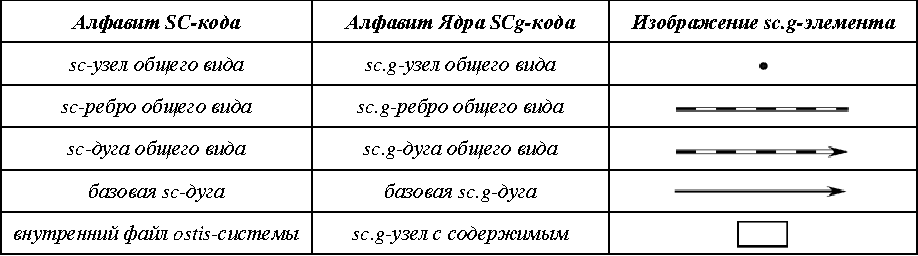
\includegraphics{figures/intro/scg/SCg-core-alphabet.pdf}\\}

%TODO сверить пропорции sc.g-элементов и изменить описание
\scnheader{sc.g-узел общего вида}
\scnidtf{\textit{sc.g-элемент}, являющийся графическим изображением \textit{sc-узла общего вида}}
\scnexplanation{Все \textit{sc-узлы}, не являющиеся знаками файлов, в тексте (конструкции) \textit{Ядра SCg-кода}, изображаются в виде небольших чёрных кругов одинакового диаметра, который обозначим через $\bm{d}$, и точная величина которого зависит от масштаба отображения \textit{sc.g-текста}.}

\scnheader{sc.g-ребро общего вида}
\scnidtf{\textit{sc.g-элемент}, являющийся графическим изображением \textit{sc-ребра общего вида}}
\scnexplanation{Каждое \textit{sc-ребро} в \textit{Ядре SCg-кода} изображается в виде широкой линии, в которой чередуются фрагменты со сплошной заливкой и без заливки, не имеющей самопересечений и имеющей общую толщину, равную примерно $\bm{0.7d}$.}

\scnheader{sc.g-дуга общего вида}
\scnidtf{\textit{sc.g-элемент}, являющийся графическим изображением \textit{sc-дуги общего вида}}
\scnexplanation{Каждая \textit{sc-дуга} в \textit{Ядре SCg-кода} изображается в виде широкой линии, в которой чередуются фрагменты со сплошной заливкой и без заливки, не имеющей самопересечений, имеющей общую толщину, равную примерно $\bm{0.7d}$ и имеющей изображение стрелочки на одном из концов этой линии.}

\scnheader{базовая sc.g-дуга}
\scnidtf{\textit{sc.g-элемент}, являющийся графическим изображением \textit{базовой sc-дуги}}
\scnexplanation{Каждая входящая в состав sc-текста \textit{базовая sc-дуга} в \textit{Ядре SCg-кода} изображается в виде линии произвольной формы, не имеющий самопересечений, имеющий толщину $\bm{0.4d}$, и имеющей изображение стрелочки на одном из ее концов.}

\scnheader{внутренний файл ostis-системы}
\scnidtf{sc-узел с содержимым}
\scnaddlevel{1}
\scniselement{часто используемый sc-идентификатор}
\scnaddlevel{-1}
\scnidtf{sc-узел, являющийся знаком внутреннего файла ostis-системы}
\scnidtf{sc-знак внутреннего файла ostis-системы}

\scnheader{sc.g-узел с содержимым}
\scnidtf{sc.g-узел, имеющий содержимое}
\scnidtf{sc.g-узел, являющийся знаком внутреннего файла ostis-системы}
\scnidtf{sc.g-знак внутреннего файла ostis-системы}
\scnidtf{sc.g-рамка, ограничивающая изображение (представление) внутреннего файла ostis-системы, обозначаемого этой sc.g-рамкой}
\scnidtf{sc.g-рамка}
\scnaddlevel{1}
\scnnote{\textit{sc.g-рамка} -- это всегда прямоугольник, максимальный размер которого не ограничивается, но минимальный фиксируется и соответствует \textit{sc.g-рамке}, внутри которой обозначаемый ею \textit{файл} не отображается.}
\scnaddlevel{-1}
\scnexplanation{Каждый входящий в sc-текст \textit{sc-узел, имеющий содержимое}, в \textit{Ядре SCg-кода} изображается в виде прямоугольника произвольного размера с толщиной линии $\bm{0.6d}$. Внутри этого прямоугольника отображается \textit{файл}, обозначаемый изображаемым \textit{sc-узлом}. Если нет необходимости изображать в тексте сам \textit{файл}, то \textit{sc-узел}, обозначающий такой \textit{файл}, в \textit{sc.g-тексте} изображается в виде прямоугольника со сторонами $\bm{2d}$ по вертикали и $\bm{4d}$ по горизонтали.}

\scnheader{Алфавит Ядра SCg-кода}
\scnnote{Трудно сразу поверить, что на основе такого простого алфавита можно построить удобный и \uline{универсальный} графовый язык. В рамках \textit{Документации Технологии OSTIS} мы постараемся Вас в этом убедить. Кроме того, нас не должна настораживать простота алфавита, поскольку человечество имеет большой опыт кодирования, хранения в памяти и передачи по каналам связи самых различных информационных ресурсов, используя алфавит, состоящий только из двух классов элементов -- единиц и нулей. 

Мы ведем речь о принципиально ином (графовом) способе кодирования информации в \textit{компьютерных системах}, но стараемся при этом свести это кодирование к достаточно простому алфавиту хотя бы для того, чтобы искусственно не усложнять проблему создания нового поколения компьютеров, основанных на указанном способе кодирования информации. 

Расширения \textit{Ядра SCg-кода} рассмотрим как направления перехода от текстов \textit{Ядра SCg-кода} к более компактным текстам. Но, поскольку это приводит к усложнению \textit{Синтаксиса SCg-кода} и, в первую очередь, к расширению \textit{Алфавита SCg-кода}, делать такие расширения необходимо обоснованно с учетом частоты встречаемости в рамках \textit{баз знаний ostis-систем} соответствующих фрагментов.}

\bigskip
\scnendstruct \scnendsegmentcomment{Описание Ядра SCg-кода}

\scnsegmentheader{Описание Первого направления расширения Ядра SCg-кода}
\scnstartsubstruct

\scnheader{Первое направление расширения Ядра SCg-кода}

\scnexplanation{\textit{Первое направление синтаксического расширения Ядра SCg-кода} -- это \uline{приписывание} некоторым \mbox{sc.g-элементам} \textit{основных sc-идентификаторов*} (чаще всего - строковых идентификаторов, то есть имен) \textit{sc-элементов} , изображаемых этими \textit{sc.g-элементами}. Указываемые идентификаторы являются уникальным для каждого идентифицируемого (именуемого) \textit{sc.g-элемента}. Приписывание \textit{sc.g-элементам} уникальных идентификаторов дает возможность в рамках одного \textit{sc.g-текста} дублировать (копировать) некоторые \textit{sc.g-узлы} при условии, если \uline{всем} таким копиям будут приписаны соответствующие идентификаторы. Такое дублирование \textit{sc.g-узлов} является дополнительным средствам \uline{наглядного} размещения \textit{sc.g-текстов}. Кроме того, приписывание \textit{sc.g-элементу} соответствующего ему основного (уникального) \textit{sc-идентификатора*} представляет собой более компактный вариант изображения \textit{sc.g-текстов}.}

\newpage
\scnheader{Пример sc.g-текста, трансформируемого по Первому направлению расширения Ядра SCg-кода}
\scneqscg{figures/intro/scg/scg_transf1.png}
\scniselement{sc.g-текст}
\scnexplanation{Здесь (в левом нижнем углу приведенного sc.g-текста) представлен \textit{sc.g-узел общего вида}, изображающий \textit{sc-узел общего вида}, которому соответствует \textit{основной sc-идентификатор*} в виде строки ``\textbf{\textit{ei}}''}
\scnrelfrom{трансформация sc.g-текста по Первому направлению расширения Ядра SCg-кода}{\scnfilescg{figures/intro/scg/scg_transf2.png}}
\scnaddlevel{1}
    \scniselement{sc.g-текст}
    \scnexplanation{\textit{sc.g-узлу общего вида} изображающему \textit{sc-узел}, внешним идентификатором которого является строка ``\textit{основной sc-идентификатор*}'' и который, соответственно является знаком \textit{бинарного ориентированного отношения}, каждая \textit{пара} которого связывает идентифицируемый \textit{sc-элемент} с его основным внешним sc-идентификатором, приписывается указанный внешний идентификатор изображаемого им \textit{sc-элемента}.}
    \scnrelfrom{трансформация sc.g-текста по Первому направлению расширения Ядра SCg-кода}{\scnfilescg{figures/intro/scg/scg_transf3.png}}
    \scnaddlevel{1}
        \scniselement{sc.g-текст} 
        \scnexplanation{В результате данной трансформации исходный \mbox{\textit{sc.g-текст}} трансформируется в один \textit{sc.g-общего вида}, которому приписывается \textit{основной sc-идентификатор} ``\textit{\textbf{ei}}''.}
    \scnaddlevel{-1}
\scnaddlevel{-1}


\scnheader{трансформация sc.g-текста по Первому направлению расширения Ядра SCg-кода*}
\scnidtf{Бинарное ориентированное отношение, каждая пара которого связывает исходный вид трансформируемого sc.g-текста и результат этой трансформации}
\scnnote{Подчеркнем, что рассматриваемая трансформация преобразует исходный текст Ядра \textit{SCg-кода} в текст, семантически эквивалентный, но принадлежащий не Ядру \textit{SCg-кода}, а его расширению.
}

\scnheader{синтаксическая трансформация*}
\scnidtf{синтаксическая трансформация информационной конструкции*}
\scnsuperset{синтаксическая трансформация sc.g-текста*}
\scnaddlevel{1}
\scnsuperset{трансформация sc.g-текста по Первому направлению расширения Ядра SCg-кода*}
\scnaddlevel{-1}

\bigskip
\scnendstruct \scnendsegmentcomment{Описание первого направления расширения Ядра SCg-кода}

\newpage
\scnsegmentheader{Описание Второго направления расширения Ядра SCg-кода}
\scnstartsubstruct

\scnheader{Второе направление расширения Ядра SCg-кода}
\scnexplanation{\textit{Второе направление расширения Ядра SCg-кода} -- это уточнение типологии \textit{константных постоянных сущностей} и расширение \textit{Алфавита Ядра SCg-кода}, позволяющее типологию \textit{константных постоянных сущностей} привести в соответствие с синтаксической типологией новых вводимых элементов \textit{Алфавита SCg-кода}. Рассмотрим подробнее sc.g-элементы, знаки \textit{константных постоянных сущностей} различного вида. Графическим признаком \textit{константных постоянных sc-узлов} в конструкциях SCg-кода является их изображение в виде \uline{окружностей} диаметра $3d$, где $d$ -- диаметр sc.g-узла общего вида. Такое изображение является более компактной записью факта принадлежности заданного sc-узла (назовем его $\bm{vi}$) классу sc-констант и классу обозначений постоянных сущностей. Запись этого факта в \textit{Ядре SCg-кода} потребует (1) явного изображения sc-узла, обозначающего класс всевозможных константных sc-элементов (класс \textit{sc-констант}), (2) явного изображения базовой sc-дуги, соединяющего изображение sc-узла, обозначающего класс sc-констант, с изображением заданного константного sc-узла, (3) явного изображение sc-узла, обозначающего класс всевозможных sc-элементов, обозначающих \textit{постоянные сущности}, (4) явного изображения базовой sc-дуги, соединяющего изображение sc-узла, обозначающего класс обозначений \textit{постоянных сущностей} с изображением рассматриваемого sc-узла $\bm{vi}$ (Смотрите \textit{Файл. Изображение спецификации sc.g-элемента средствами Ядра SCg-кода и Первого расширения Ядра SCg-кода}).

Общепринятая запись данного факта выглядит следующим образом:

``\textit{sc-константа} $\ni \bm{vi}$; \textit{постоянная сущность} $\ni \bm{v_i};$''

\textit{Константные постоянные sc-ребра} в конструкциях SCg-кода изображаются в виде двойной линии, каждая из которых имеет толщину примерно $d/7$, а расстояние между ними равно примерно $3d/7$. 

\textit{Константные постоянные sc-дуги} изображаются в виде такой же двойной линии, но со стрелочкой. Все \textit{базовые sc-дуги}, а также все sc-узлы, имеющие содержимое, по определению являются \textit{константными постоянными sc-элементами}. 

\textit{Константные sc.g-узлы}, изображаемые окружностями диаметра $3d$ и толщиной границы $d/5$, обозначают \textit{константные постоянные сущности}, о которых мало что известно, но известно то, что они не являются парами (то есть множествами, \textit{мощность*} которых равна 2) и, следовательно, не могут быть изображёны в виде sc.g-дуг или sc.g-рёбер. Но, если при этом об обозначаемой \textit{константной постоянной сущности} ($\bm{vi}$) известно, что она является классом сущностей, то явное указание принадлежности sc-элемента \textit{vi} всевозможных классов можно заменить на специальное графическое изображение sc-элемента \textit{vi}, предполагаемое указанную принадлежность. Это приводит к расширению  \textit{Алфавита SCg-кода} (см. \textit{Примеры sc.g-текстов, трансформируемых по Второму направлению расширения Ядра SCg-код}).

Аналогичным образом (см. \textit{Примеры sc.g-текстов, трансформируемых по Второму направлению расширения Ядра SCg-код}) вводятся: 
\begin{scnitemize}
\item sc.g-узел, являющийся изображением \textit{класса};  
\item sc.g-узел, являющийся изображением \textit{класса классов};  
\item sc.g-узел, являющийся изображением \textit{отношения}; 
\item sc.g-узел, являющийся изображением \textit{ролевого отношения}; 
\item sc.g-узел, являющийся изображением \textit{структуры};  
\item sc.g-узел, являющийся изображением \textit{небинарной связки};
\item sc.g-узел, являющийся изображением \textit{первичной сущности} (терминальной сущности, которая не является множеством, а также файлом, хранимым в памяти ostis-системы).
\end{scnitemize}

Важное место среди константных постоянных сущностей занимают \textit{константные постоянные пары принадлежности}, обозначаемое соответствующими \textit{sc.g-дугами}. Такие пары принадлежности и обозначающие их sc.g-дуги бывают позитивными, негативными и нечеткими. Константная постоянная позитивная sc.g-дуга принадлежности есть ничто иное, как \textit{базовая sc.g-дуга}. Константная постоянная негативная sc.g-дуга принадлежности изображается в виде \textit{базовой sc.g-дуги}, перечеркнутой штриховыми черточками. Константная постоянная нечёткая sc.g-дуга принадлежности изображается в виде "недочеркнутой"{} \textit{базовой sc.g-дуги}, с каждой стороны которой отображаются штрихи, по длине равные половине от длины штрихов, которыми перечеркнута \textit{константная постоянная негативная sc.g-дуга}.}

\scnheader{Файл. Изображение спецификации sc.g-элемента средствами Ядра SCg-кода и Второго направления расширения Ядра SCg-кода}
\scneqscg{figures/intro/scg/scg2ex.png}

\scnheader{Примеры sc.g-текстов, трансформируемых по Второму направлению расширения Ядра SCg-кода}
\scnstructinclusion

\scnmakeset{\scgfileitem{figures/intro/scg/scg2_ex1.png}\\
\scnaddlevel{1}
    \scnrelfrom{синтаксическая трансформация}{\scnfilescg{figures/intro/scg/scg2_ex1_1.png}}
    \scnaddlevel{1}
        \scnexplanation{Здесь вводится новый синтаксический вид \textit{sc.g-элементов} -- \textit{константный постоянный sc.g-узел общего вида}, изображаемый окружностью диаметра $3d$ и толщиной границы $d/5$.}
    \scnaddlevel{-1}
\scnaddlevel{-1};
\scgfileitem{figures/intro/scg/nodes/const_perm/scg_const_perm_class1.png}\\
\scnaddlevel{1}
    \scnrelfrom{синтаксическая трансформация}{\scnfilescg{figures/intro/scg/nodes/const_perm/scg_const_perm_class2.png}}
    \scnaddlevel{1}
        \scnexplanation{Здесь вводится новый синтаксический вид \textit{sc.g-элементов} -- \textit{константный постоянный sc.g-узел, обозначающий класс}, изображаемый как \textit{константный постоянный sc.g-узел} с "решеткой"{} внутри.}
    \scnaddlevel{-1}
\scnaddlevel{-1}
\newpage;
\scgfileitem{figures/intro/scg/nodes/const_perm/scg_const_perm_class_of_classes1.png}\\
\scnaddlevel{1}
    \scnrelfrom{синтаксическая трансформация}{\scnfilescg{figures/intro/scg/nodes/const_perm/scg_const_perm_class_of_classes2.png}}
    \scnaddlevel{1}
        \scnexplanation{Здесь вводится новый синтаксический вид \textit{sc.g-элементов} -- \textit{константный постоянный \mbox{sc.g-узел}, обозначающий класс классов}, изображаемый как \textit{константный постоянный \mbox{sc.g-узел}} с направленным вверх углом внутри.}
    \scnaddlevel{-1}
\scnaddlevel{-1};
\scgfileitem{figures/intro/scg/nodes/const_perm/scg_const_perm_norole1.png}\\
\scnaddlevel{1}
    \scnrelfrom{синтаксическая трансформация}{\scnfilescg{figures/intro/scg/nodes/const_perm/scg_const_perm_norole2.png}}
    \scnaddlevel{1}
        \scnexplanation{Здесь вводится новый синтаксический вид \textit{sc.g-элементов} -- \textit{константный постоянный \mbox{sc.g-узел}, обозначающий неролевое отношение}, изображаемый как \textit{константный постоянный sc.g-узел} с "крестиком"{} внутри.}
    \scnaddlevel{-1}
\scnaddlevel{-1};
\scgfileitem{figures/intro/scg/nodes/const_perm/scg_const_perm_role1.png}\\
\scnaddlevel{1}
    \scnrelfrom{синтаксическая трансформация}{\scnfilescg{figures/intro/scg/nodes/const_perm/scg_const_perm_role2.png}}
    \scnaddlevel{1}
        \scnexplanation{Здесь вводится новый синтаксический вид \textit{sc.g-элементов} -- \textit{константный постоянный sc.g-узел, обозначающий ролевое отношение}, изображаемый как \textit{константный постоянный sc.g-узел} с "плюсом"{} внутри.}
    \scnaddlevel{-1}
\scnaddlevel{-1}
\newpage;
\scgfileitem{figures/intro/scg/nodes/const_perm/scg_const_perm_structure1.png}\\
\scnaddlevel{1}
    \scnrelfrom{синтаксическая трансформация}{\scnfilescg{figures/intro/scg/nodes/const_perm/scg_const_perm_structure2.png}}
    \scnaddlevel{1}
        \scnexplanation{Здесь вводится новый синтаксический вид \textit{sc.g-элементов} -- \textit{константный постоянный \mbox{sc.g-узел}, обозначающий структуру}, изображаемый как \textit{константный постоянный \mbox{sc.g-узел}} с точкой внутри.}
    \scnaddlevel{-1}
\scnaddlevel{-1};
\scgfileitem{figures/intro/scg/nodes/const_perm/scg_const_perm_primary_entity1.png}\\
\scnaddlevel{1}
    \scnrelfrom{синтаксическая трансформация}{\scnfilescg{figures/intro/scg/nodes/const_perm/scg_const_perm_primary_entity2.png}}
    \scnaddlevel{1}
        \scnexplanation{Здесь вводится новый синтаксический вид \textit{sc.g-элементов} -- \textit{константный постоянный \mbox{sc.g-узел}, обозначающий первичную сущность}, изображаемый как \textit{константный постоянный \mbox{sc.g-узел}} с  косой штриховкой внутри.}
    \scnaddlevel{-1}
\scnaddlevel{-1};
\scgfileitem{figures/intro/scg/nodes/const_perm/scg_const_perm_tuple1.png}\\
\scnaddlevel{1}
    \scnrelfrom{синтаксическая трансформация}{\scnfilescg{figures/intro/scg/nodes/const_perm/scg_const_perm_tuple2.png}}
    \scnaddlevel{1}
        \scnexplanation{Здесь вводится новый синтаксический вид \textit{sc.g-элементов} -- \textit{константный постоянный \mbox{sc.g-узел}, обозначающий небинарную связку}, изображаемый как \textit{константный постоянный sc.g-узел} с горизонтальной линией внутри.}
    \scnaddlevel{-1}
\scnaddlevel{-1}
\newpage;
\scgfileitem{figures/intro/scg/arcs/const/scg_const_perm_noorien1.png}\\
\scnaddlevel{1}
    \scnrelfrom{синтаксическая трансформация}{\scnfilescg{figures/intro/scg/arcs/const/scg_const_perm_noorien2.png}}
    \scnaddlevel{1}
        \scnexplanation{Здесь вводится новый синтаксический вид \textit{sc.g-элементов} -- \textit{константное постоянное sc.g-ребро}, изображаемое двумя непрерывными параллельными линиями.}
    \scnaddlevel{-1}
\scnaddlevel{-1};
\scgfileitem{figures/intro/scg/arcs/const/scg_const_perm_orient1.png}\\
\scnaddlevel{1}
    \scnrelfrom{синтаксическая трансформация}{\scnfilescg{figures/intro/scg/arcs/const/scg_const_perm_orient2.png}}
    \scnaddlevel{1}
        \scnexplanation{Здесь вводится новый синтаксический вид \textit{sc.g-элементов} -- \textit{константная постоянная \mbox{sc.g-дуга}}, изображаемая двумя непрерывными параллельными линиями с общей стрелкой на одном из концов.}
    \scnaddlevel{-1}
\scnaddlevel{-1};
\scgfileitem{figures/intro/scg/arcs/const/scg_const_perm_positive1.png}\\
\scnaddlevel{1}
    \scnrelfrom{синтаксическая трансформация}{\scnfilescg{figures/intro/scg/arcs/const/scg_const_perm_positive2.png}}
    \scnaddlevel{1}
        \scnexplanation{\textit{Константная постоянная позитивная sc.g-дуга принадлежности} есть ничто иное, как \textit{базовая sc.g-дуга}.}
    \scnaddlevel{-1}
\scnaddlevel{-1}
\newpage;
\scgfileitem{figures/intro/scg/arcs/const/scg_const_perm_negative1.png}\\
\scnaddlevel{1}
    \scnrelfrom{синтаксическая трансформация}{\scnfilescg{figures/intro/scg/arcs/const/scg_const_perm_negative2.png}}
    \scnaddlevel{1}
        \scnexplanation{Здесь вводится новый синтаксический вид \textit{sc.g-элементов} -- \textit{константная постоянная негативная sc.g-дуга принадлежности}, изображается в виде \textit{базовой sc.g-дуги}, перечеркнутой штриховыми черточками.}
    \scnaddlevel{-1}
\scnaddlevel{-1};
\scgfileitem{figures/intro/scg/arcs/const/scg_const_perm_fuzzy1.png}\\
\scnaddlevel{1}
    \scnrelfrom{синтаксическая трансформация}{\scnfilescg{figures/intro/scg/arcs/const/scg_const_perm_fuzzy2.png}}
    \scnaddlevel{1}
        \scnexplanation{Здесь вводится новый синтаксический вид \textit{sc.g-элементов} -- \textit{константная постоянная нечеткая sc.g-дуга принадлежности}, которая изображается в виде "недочеркнутой"{} \textit{базовой sc.g-дуги}, с каждой стороны которой отображаются штрихи, по длине равные половине от длины штрихов, которыми перечеркнута \textit{константная постоянная негативная sc.g-дуга}.}
    \scnaddlevel{-1}
\scnaddlevel{-1}
}

\newpage
\scnheader{Примеры sc.g-текста, записанного средствами Второго направления расширения Ядра SCg-кода}
\scnstructinclusion

\scnmakeset{\scgfileitem{figures/intro/scg/examples/scg_example_triangle.png}
\scnaddlevel{1}
\scniselementrole{пример}{sc.g-текст}
\scnexplanation{Данный sc.g-текст содержит следующую информацию:
\begin{scnitemize}
\item Сущности \textit{Треугольник ABC}~~ и ~~\textit{Треугольник CDE} являются треугольниками (принадлежат классу \textit{треугольников}). При этом известно, что площадь \textit{Треугольника CDE} в 4 раза больше, чем площадь \textit{Треугольника ABC}, но конкретные значения ллощадей не известны\char59
\item Сущность \textit{Отрезок DE} является отрезком (принадлежит классу \textit{отрезков}) и является стороной \textit{Треугольника CDE}. Кроме того, у \textit{Отрезка DE} есть длина, измерение которой в сантиметрах составляет 5. Обратите внимание, что в данном случае для упрощения понимания использовано бинарное отношение \textit{длина*}, которое является \textit{неосновным понятием} и в базе знаний заменяется на \textit{базовую sc-дугу}, связывающую величину как класс эквивалентности с конкретной сущностью, входящей в данный класс, в данном случае -- \textit{Отрезок DE}\char59  
\item Сущность \textit{Треугольник AEB} является треугольником и имеет \textit{внутренний угол*}~~~ \textit{Угол AEB}. В свою очередь, \textit{Угол AEB} является \textit{углом} и имеет \textit{косинус*}, равный 0,5\char59
\item \textit{Треугольник AEB} имеет \textit{сторону*} (не указывается, какая именно из сторон имеется в виду), \textit{средней точкой*} которой является \textit{Точка O}. В свою очередь, \textit{Точка O} является центром некоторой \textit{Окружности O}, которая относится к классу \textit{окружностей}.
\end{scnitemize}
}\scnaddlevel{-1}
\newpage;
\scgfileitem{figures/intro/scg/examples/scg_example_alice.png}
\newpage
\scnaddlevel{1}
	\scnexplanation{Данный sc.g-текст основан на популярном примере, наглядно иллюстрируещем понятие семантической сети, известном как ``Социальная сеть Алисы''. Как видно из примера, данный текст описывает различные взаимосвязи персоны по имени Алиса, при этом некоторые из используемых отношений является ориентированными (например, ``работник*''), а некоторые -- неориентированными (например, ``друг*'').}
\scnaddlevel{-1}
}

\bigskip
\scnendstruct \scnendsegmentcomment{Описание Второго направления расширения Ядра SCg-кода}

\scnsegmentheader{Описание Третьего направления расширения Ядра SCg-кода}

\scnstartsubstruct

\scnheader{Третье направление расширения Ядра SCg-кода}
\scnexplanation{\textit{Третье направление расширения Ядра SCg-кода} -- это расширение его алфавита путем введения дополнительных sc.g-элементов, обозначающих \textit{константные временные сущности} различного вида. Признаком sc.g-элементов, обозначающих \textit{константные временные сущности} являются точечные линии (линии, состоящие из точек, размер которых равен размеру изображаемой линии и которые близко расположены друг к другу на расстоянии, равном половине их размера), с помощью которых рисуются окружности при изображении sc-узлов, а также линии при изображении sc-коннекторов.

Результатом \textit{Третьего направления расширения Ядра SCg-кода} является введение следующих видов sc.g-элементов (см. \textit{Примеры sc.g-текстов, трансформируемых по Третьему направлению расширения Ядра SCg-кода}).}

\scnheader{Примеры sc.g-текстов, трансформируемых по Третьему направлению расширения Ядра SCg-кода}
\scnstructinclusion
\scnmakeset{\scgfileitem{figures/intro/scg/nodes/const_temp/scg_const_temp_general_view1.png}\\
\scnaddlevel{1}
    \scnrelfrom{синтаксическая трансформация}{\scnfilescg{figures/intro/scg/nodes/const_temp/scg_const_temp_general_view2.png}}
    \scnaddlevel{1}
        \scnexplanation{Здесь вводится новый синтаксический вид \textit{sc.g-элементов} -- \textit{константный временный \mbox{sc.g-узел общего вида}}, изображаемый точечной окружностью диаметра $3d$ и толщиной границы $d/5$.}
    \scnaddlevel{-1}
\scnaddlevel{-1};
\scgfileitem{figures/intro/scg/nodes/const_temp/scg_const_temp_class1.png}\\
\scnaddlevel{1}
    \scnrelfrom{синтаксическая трансформация}{\scnfilescg{figures/intro/scg/nodes/const_temp/scg_const_temp_class2.png}}
    \scnaddlevel{1}
        \scnexplanation{Здесь вводится новый синтаксический вид \textit{sc.g-элементов} -- \textit{константный временный \mbox{sc.g-узел}, обозначающий класс}, изображаемый как \textit{константный временный \mbox{sc.g-узел}} с "решеткой"{} внутри.}
    \scnaddlevel{-1}
\scnaddlevel{-1};
\scgfileitem{figures/intro/scg/nodes/const_temp/scg_const_temp_class_of_classes1.png}\\
\scnaddlevel{1}
    \scnrelfrom{синтаксическая трансформация}{\scnfilescg{figures/intro/scg/nodes/const_temp/scg_const_temp_class_of_classes2.png}}
    \scnaddlevel{1}
        \scnexplanation{Здесь вводится новый синтаксический вид \textit{sc.g-элементов} -- \textit{константный временный \mbox{sc.g-узел}, обозначающий класс классов}, изображаемый как \textit{константный временный \mbox{sc.g-узел}} с направленным вверх углом внутри.}
    \scnaddlevel{-1}
\scnaddlevel{-1};
\scgfileitem{figures/intro/scg/nodes/const_temp/scg_const_temp_norole1.png}\\
\scnaddlevel{1}
    \scnrelfrom{синтаксическая трансформация}{\scnfilescg{figures/intro/scg/nodes/const_temp/scg_const_temp_norole2.png}}
    \scnaddlevel{1}
        \scnexplanation{Здесь вводится новый синтаксический вид \textit{sc.g-элементов} -- \textit{константный временный \mbox{sc.g-узел}, обозначающий неролевое отношение}, изображаемый как \textit{константный временный sc.g-узел} с "крестиком"{} внутри.}
    \scnaddlevel{-1}
\scnaddlevel{-1};
\scgfileitem{figures/intro/scg/nodes/const_temp/scg_const_temp_role1.png}\\
\scnaddlevel{1}
    \scnrelfrom{синтаксическая трансформация}{\scnfilescg{figures/intro/scg/nodes/const_temp/scg_const_temp_role2.png}}
    \scnaddlevel{1}
    \newpage
        \scnexplanation{Здесь вводится новый синтаксический вид \textit{sc.g-элементов} -- \textit{константный временный \mbox{sc.g-узел}, обозначающий ролевое отношение}, изображаемый как \textit{константный временный \mbox{sc.g-узел}} с "плюсом"{} внутри.}
    \scnaddlevel{-1}
\scnaddlevel{-1};
\scgfileitem{figures/intro/scg/nodes/const_temp/scg_const_temp_structure1.png}\\
\scnaddlevel{1}
    \scnrelfrom{синтаксическая трансформация}{\scnfilescg{figures/intro/scg/nodes/const_temp/scg_const_temp_structure2.png}}
    \scnaddlevel{1}
        \scnexplanation{Здесь вводится новый синтаксический вид \textit{sc.g-элементов} -- \textit{константный временный \mbox{sc.g-узел}, обозначающий структуру}, изображаемый как \textit{константный временный \mbox{sc.g-узел}} с точкой внутри.}
    \scnaddlevel{-1}
\scnaddlevel{-1};
\scgfileitem{figures/intro/scg/nodes/const_temp/scg_const_temp_primary_entity1.png}\\
\scnaddlevel{1}
    \scnrelfrom{синтаксическая трансформация}{\scnfilescg{figures/intro/scg/nodes/const_temp/scg_const_temp_primary_entity2.png}}
    \scnaddlevel{1}
        \scnexplanation{Здесь вводится новый синтаксический вид \textit{sc.g-элементов} -- \textit{константный временный \mbox{sc.g-узел}, обозначающий первичную сущность}, изображаемый как \textit{константный временный \mbox{sc.g-узел}} с косой штриховкой внутри.}
    \scnaddlevel{-1}
\scnaddlevel{-1};
\scgfileitem{figures/intro/scg/nodes/const_temp/scg_const_temp_tuple1.png}\\
\scnaddlevel{1}
    \scnrelfrom{синтаксическая трансформация}{\scnfilescg{figures/intro/scg/nodes/const_temp/scg_const_temp_tuple2.png}}
    \scnaddlevel{1}
    \newpage
        \scnexplanation{Здесь вводится новый синтаксический вид \textit{sc.g-элементов} -- \textit{константный временный \mbox{sc.g-узел}, обозначающий небинарную связку}, изображаемый как \textit{константный временный \mbox{sc.g-узел}} с горизонтальной линией внутри.}
    \scnaddlevel{-1}
\scnaddlevel{-1};
\scgfileitem{figures/intro/scg/arcs/const/scg_const_temp_noorien1.png}\\
\scnaddlevel{1}
    \scnrelfrom{синтаксическая трансформация}{\scnfilescg{figures/intro/scg/arcs/const/scg_const_temp_noorien2.png}}
    \scnaddlevel{1}
        \scnexplanation{Здесь вводится новый синтаксический вид \textit{sc.g-элементов} -- \textit{константное временное \mbox{sc.g-ребро}}, изображаемое двумя точечными параллельными линиями.}
    \scnaddlevel{-1}
\scnaddlevel{-1};
\scgfileitem{figures/intro/scg/arcs/const/scg_const_temp_orient1.png}\\
\scnaddlevel{1}
    \scnrelfrom{синтаксическая трансформация}{\scnfilescg{figures/intro/scg/arcs/const/scg_const_temp_orient2.png}}
    \scnaddlevel{1}
        \scnexplanation{Здесь вводится новый синтаксический вид \textit{sc.g-элементов} -- \textit{константная временная \mbox{sc.g-дуга}}, изображаемая двумя точечными параллельными линиями с общей стрелкой на одном из концов.}
    \scnaddlevel{-1}
\scnaddlevel{-1};
\scgfileitem{figures/intro/scg/arcs/const/scg_const_temp_positive1.png}\\
\scnaddlevel{1}
    \scnrelfrom{синтаксическая трансформация}{\scnfilescg{figures/intro/scg/arcs/const/scg_const_temp_positive2.png}}
    \scnaddlevel{1}
    \newpage
        \scnexplanation{Здесь вводится новый синтаксический вид \textit{sc.g-элементов} -- \textit{константная временная позитивная sc.g-дуга принадлежности}, изображаемая точечной линией со стрелкой на конце.}
    \scnaddlevel{-1}
\scnaddlevel{-1};
\scgfileitem{figures/intro/scg/arcs/const/scg_const_temp_negative1.png}\\
\scnaddlevel{1}
    \scnrelfrom{синтаксическая трансформация}{\scnfilescg{figures/intro/scg/arcs/const/scg_const_temp_negative2.png}}
    \scnaddlevel{1}
        \scnexplanation{Здесь вводится новый синтаксический вид \textit{sc.g-элементов} -- \textit{константная временная негативная sc.g-дуга принадлежности}, изображаемая точечной линией, перечеркнутой штриховыми черточками, со стрелкой на конце.}
    \scnaddlevel{-1}
\scnaddlevel{-1};
\scgfileitem{figures/intro/scg/arcs/const/scg_const_temp_fuzzy1.png}\\
\scnaddlevel{1}
    \scnrelfrom{синтаксическая трансформация}{\scnfilescg{figures/intro/scg/arcs/const/scg_const_temp_fuzzy2.png}}
    \scnaddlevel{1}
        \scnexplanation{Здесь вводится новый синтаксический вид \textit{sc.g-элементов} -- \textit{константная временная нечеткая sc.g-дуга принадлежности}, которая изображается в виде "недочеркнутой"{} \textit{\textit{константной временной позитивная sc.g-дуги принадлежности}, с каждой стороны которой отображаются штрихи, по длине равные половине от длины штрихов, которыми перечеркнута \textit{константная постоянная негативная sc.g-дуга}.}
    \scnaddlevel{-1}
{-1}}}

\bigskip
\scnendstruct \scnendsegmentcomment{Описание Третьего направления расширения Ядра SCg-кода}

\scnsegmentheader{Описание Четвёртого направления расширения Ядра SCg-кода}

\scnstartsubstruct

\scnheader{Четвёртое направление расширения Ядра SCg-кода}
\scnexplanation{\textit{Четвёртое направление расширения Ядра SCg-кода} -- это расширение его алфавита путем введения дополнительных элементов, обозначающих \textit{переменные постоянные сущности} различного вида. Признаком sc.g-элементов, обозначающих сущности указанного класса, являются квадратики для изображения обозначений \textit{переменных постоянных сущностей}, не являющихся бинарными связями, а также пунктирные и штрих-пунктирные линии для изображения \textit{переменных постоянных бинарных связей}. 

Подчеркнем, что \textit{переменные постоянные сущности} могут отличаться друг от друга по характеру их \textit{области значений*}. Этими значениями в общем случае могут быть как \textit{константные постоянные сущности}, так и \textit{переменные постоянные сущности}. В любом случае, значение \textit{переменной сущности} является либо \textit{константной сущностью}, либо \textit{переменной сущностью}. Если каждое значение переменной является константой, то такую переменную будем называть \textit{переменной первого уровня}. Если каждое значение переменной является \textit{переменной первого уровня}, то такую переменную будем называть \textit{переменной второго уровня}. 

\textit{Переменная постоянная сущность первого уровня } (первичная sc-переменная), не являющаяся бинарной связью -- это переменная, каждым значением которой является \textit{константная постоянная сущность}, не являющаяся бинарной связью. Такая переменная изображается квадратиком, который ориентирован по вертикали и горизонтали. 

\textit{переменная постоянная сущность второго уровня} (вторичная sc-переменная), не являющаяся бинарной связью, изображается квадратиком, повернутым на 45$^\circ$. 

Указанная выше семантика таких изображений приписывается \uline{по умолчанию}. Это означает, что, если обозначаемая sc-переменная имеет более сложную структуру области её значений (является sc-переменной третьего и выше уровня или sc-переменной, значения которой имеют различный логический уровень), то эта область должна быть специфицирована явно, при этом такая sc-переменная в SCg-коде изображается так же, как первичная sc-переменная.}

\scnheader{Примеры sc.g-текстов, трансформируемых по Четвертому направлению расширения Ядра SCg-кода}
\scnstructinclusion
\scnmakeset{\scgfileitem{figures/intro/scg/nodes/var_perm/scg_var_perm_general_view1.png}\\
\scnaddlevel{1}
    \scnrelfrom{синтаксическая трансформация}{\scnfilescg{figures/intro/scg/nodes/var_perm/scg_var_perm_general_view2.png}}
    \scnaddlevel{1}
        \scnexplanation{Здесь вводится новый синтаксический вид \textit{sc.g-элементов} -- \textit{переменный постоянный \mbox{sc.g-узел} общего вида}, изображаемый квадратиком cj со стороной длины $3d$ и толщиной границы $d/5$.}
    \scnaddlevel{-1}
\scnaddlevel{-1};
\scgfileitem{figures/intro/scg/nodes/var_perm/scg_var_perm_class1.png}\\
\scnaddlevel{1}
    \scnrelfrom{синтаксическая трансформация}{\scnfilescg{figures/intro/scg/nodes/var_perm/scg_var_perm_class2.png}}
    \scnaddlevel{1}
        \scnexplanation{Здесь вводится новый синтаксический вид \textit{sc.g-элементов} -- \textit{переменный постоянный sc.g-узел, обозначающий класс}, изображаемый как \textit{переменный постоянный sc.g-узел} с "решеткой"{} внутри.}
    \scnaddlevel{-1}
\scnaddlevel{-1}
\newpage;
\scgfileitem{figures/intro/scg/nodes/var_perm/scg_var_perm_class_of_classes1.png}\\
\scnaddlevel{1}
    \scnrelfrom{синтаксическая трансформация}{\scnfilescg{figures/intro/scg/nodes/var_perm/scg_var_perm_class_of_classes2.png}}
    \scnaddlevel{1}
        \scnexplanation{Здесь вводится новый синтаксический вид \textit{sc.g-элементов} -- \textit{переменный постоянный \mbox{sc.g-узел}, обозначающий класс классов}, изображаемый как \textit{переменный постоянный \mbox{sc.g-узел}} с направленным вверх углом внутри.}
    \scnaddlevel{-1}
\scnaddlevel{-1};
\scgfileitem{figures/intro/scg/nodes/var_perm/scg_var_perm_norole1.png}\\
\scnaddlevel{1}
    \scnrelfrom{синтаксическая трансформация}{\scnfilescg{figures/intro/scg/nodes/var_perm/scg_var_perm_norole2.png}}
    \scnaddlevel{1}
        \scnexplanation{Здесь вводится новый синтаксический вид \textit{sc.g-элементов} -- \textit{переменный постоянный \mbox{sc.g-узел}, обозначающий неролевое отношение}, изображаемый как \textit{переменный постоянный \mbox{sc.g-узел}} с "крестиком"{} внутри.}
    \scnaddlevel{-1}
\scnaddlevel{-1};
\scgfileitem{figures/intro/scg/nodes/var_perm/scg_var_perm_role1.png}\\
\scnaddlevel{1}
    \scnrelfrom{синтаксическая трансформация}{\scnfilescg{figures/intro/scg/nodes/var_perm/scg_var_perm_role2.png}}
    \scnaddlevel{1}
        \scnexplanation{Здесь вводится новый синтаксический вид \textit{sc.g-элементов} -- \textit{переменный постоянный sc.g-узел, обозначающий ролевое отношение}, изображаемый как \textit{переменный постоянный sc.g-узел} с "плюсом"{} внутри.}
    \scnaddlevel{-1}
\scnaddlevel{-1}
\newpage;
\scgfileitem{figures/intro/scg/nodes/var_perm/scg_var_perm_structure1.png}\\
\scnaddlevel{1}
    \scnrelfrom{синтаксическая трансформация}{\scnfilescg{figures/intro/scg/nodes/var_perm/scg_var_perm_structure2.png}}
    \scnaddlevel{1}
        \scnexplanation{Здесь вводится новый синтаксический вид \textit{sc.g-элементов} -- \textit{переменный постоянный \mbox{sc.g-узел}, обозначающий структуру}, изображаемый как \textit{переменный постоянный \mbox{sc.g-узел}} с точкой внутри.}
    \scnaddlevel{-1}
\scnaddlevel{-1};
\scgfileitem{figures/intro/scg/nodes/var_perm/scg_var_perm_primary_entity1.png}\\
\scnaddlevel{1}
    \scnrelfrom{синтаксическая трансформация}{\scnfilescg{figures/intro/scg/nodes/var_perm/scg_var_perm_primary_entity2.png}}
    \scnaddlevel{1}
        \scnexplanation{Здесь вводится новый синтаксический вид \textit{sc.g-элементов} -- \textit{переменный постоянный \mbox{sc.g-узел}, обозначающий первичную сущность}, изображаемый как \textit{переменный постоянный \mbox{sc.g-узел}} с  косой штриховкой внутри.}
    \scnaddlevel{-1}
\scnaddlevel{-1};
\scgfileitem{figures/intro/scg/nodes/var_perm/scg_var_perm_tuple1.png}\\
\scnaddlevel{1}
    \scnrelfrom{синтаксическая трансформация}{\scnfilescg{figures/intro/scg/nodes/var_perm/scg_var_perm_tuple2.png}}
    \scnaddlevel{1}
        \scnexplanation{Здесь вводится новый синтаксический вид \textit{sc.g-элементов} -- \textit{переменный постоянный \mbox{sc.g-узел}, обозначающий небинарную связку}, изображаемый как \textit{переменный постоянный \mbox{sc.g-узел}} с горизонтальной линией внутри.}
    \scnaddlevel{-1}
\scnaddlevel{-1}
\newpage;
\scgfileitem{figures/intro/scg/arcs/var/scg_var_perm_noorien1.png}\\
\scnaddlevel{1}
    \scnrelfrom{синтаксическая трансформация}{\scnfilescg{figures/intro/scg/arcs/var/scg_var_perm_noorien2.png}}
    \scnaddlevel{1}
        \scnexplanation{Здесь вводится новый синтаксический вид \textit{sc.g-элементов} -- \textit{переменное постоянное \mbox{sc.g-ребро}}, изображаемое двумя пунктирными параллельными линиями.}
    \scnaddlevel{-1}
\scnaddlevel{-1};
\scgfileitem{figures/intro/scg/arcs/var/scg_var_perm_orient1.png}\\
\scnaddlevel{1}
    \scnrelfrom{синтаксическая трансформация}{\scnfilescg{figures/intro/scg/arcs/var/scg_var_perm_orient2.png}}
    \scnaddlevel{1}
        \scnexplanation{Здесь вводится новый синтаксический вид \textit{sc.g-элементов} -- \textit{переменная постоянная sc.g-дуга}, изображаемая двумя пунктирными параллельными линиями с общей стрелкой на одном из концов.}
    \scnaddlevel{-1}
\scnaddlevel{-1};
\scgfileitem{figures/intro/scg/arcs/var/scg_var_perm_positive1.png}\\
\scnaddlevel{1}
    \scnrelfrom{синтаксическая трансформация}{\scnfilescg{figures/intro/scg/arcs/var/scg_var_perm_positive2.png}}
    \scnaddlevel{1}
        \scnexplanation{\textit{переменная постоянная позитивная sc.g-дуга принадлежности}, изображаемая пунктирной линией со стрелкой на конце.}
    \scnaddlevel{-1}
\scnaddlevel{-1}
\newpage;
\scgfileitem{figures/intro/scg/arcs/var/scg_var_perm_negative1.png}\\
\scnaddlevel{1}
    \scnrelfrom{синтаксическая трансформация}{\scnfilescg{figures/intro/scg/arcs/var/scg_var_perm_negative2.png}}
    \scnaddlevel{1}
        \scnexplanation{Здесь вводится новый синтаксический вид \textit{sc.g-элементов} -- \textit{переменная постоянная негативная sc.g-дуга принадлежности}, изображается в виде \textit{переменной постоянной позитивной sc.g-дуги принадлежности}, перечеркнутой штриховыми черточками.}
    \scnaddlevel{-1}
\scnaddlevel{-1};
\scgfileitem{figures/intro/scg/arcs/var/scg_var_perm_fuzzy1.png}\\
\scnaddlevel{1}
    \scnrelfrom{синтаксическая трансформация}{\scnfilescg{figures/intro/scg/arcs/var/scg_var_perm_fuzzy2.png}}
    \scnaddlevel{1}
        \scnexplanation{Здесь вводится новый синтаксический вид \textit{sc.g-элементов} -- \textit{переменная постоянная нечеткая sc.g-дуга принадлежности}, которая изображается в виде "недочеркнутой"{} \textit{переменной постоянной позитивной sc.g-дуги принадлежности}, с каждой стороны которой отображаются штрихи, по длине равные половине от длины штрихов, которыми перечеркнута \textit{переменная постоянная негативная sc.g-дуга}.}
    \scnaddlevel{-1}
\scnaddlevel{-1};
\scgfileitem{figures/intro/scg/nodes/metavar_perm/scg_metavar_perm_general_view1.png}\\
\scnaddlevel{1}
    \scnrelfrom{синтаксическая трансформация}{\scnfilescg{figures/intro/scg/nodes/metavar_perm/scg_metavar_perm_general_view2.png}}
    \scnaddlevel{1}
        \scnexplanation{Здесь вводится новый синтаксический вид \textit{sc.g-элементов} -- \textit{метапеременный постоянный sc.g-узел общего вида}, изображаемый квадратиком, повернутым на 45 градусов.}
    \scnaddlevel{-1}
\scnaddlevel{-1}
\newpage;
\scgfileitem{figures/intro/scg/nodes/metavar_perm/scg_metavar_perm_class1.png}\\
\scnaddlevel{1}
    \scnrelfrom{синтаксическая трансформация}{\scnfilescg{figures/intro/scg/nodes/metavar_perm/scg_metavar_perm_class2.png}}
    \scnaddlevel{1}
        \scnexplanation{Здесь вводится новый синтаксический вид \textit{sc.g-элементов} -- \textit{метапеременный постоянный sc.g-узел, обозначающий класс}, изображаемый как \textit{метапеременный постоянный sc.g-узел} с "решеткой"{} внутри.}
    \scnaddlevel{-1}
\scnaddlevel{-1};
\scgfileitem{figures/intro/scg/nodes/metavar_perm/scg_metavar_perm_class_of_classes1.png}\\
\scnaddlevel{1}
    \scnrelfrom{синтаксическая трансформация}{\scnfilescg{figures/intro/scg/nodes/metavar_perm/scg_metavar_perm_class_of_classes2.png}}
    \scnaddlevel{1}
        \scnexplanation{Здесь вводится новый синтаксический вид \textit{sc.g-элементов} -- \textit{метапеременный постоянный sc.g-узел, обозначающий класс классов}, изображаемый как \textit{метапеременный постоянный sc.g-узел} с направленным вверх углом внутри.}
    \scnaddlevel{-1}
\scnaddlevel{-1};
\scgfileitem{figures/intro/scg/nodes/metavar_perm/scg_metavar_perm_norole1.png}\\
\scnaddlevel{1}
    \scnrelfrom{синтаксическая трансформация}{\scnfilescg{figures/intro/scg/nodes/metavar_perm/scg_metavar_perm_norole2.png}}
    \scnaddlevel{1}
        \scnexplanation{Здесь вводится новый синтаксический вид \textit{sc.g-элементов} -- \textit{метапеременный постоянный sc.g-узел, обозначающий неролевое отношение}, изображаемый как \textit{метапеременный постоянный sc.g-узел} с "крестиком"{} внутри.}
    \scnaddlevel{-1}
\scnaddlevel{-1}
\newpage;
\scgfileitem{figures/intro/scg/nodes/metavar_perm/scg_metavar_perm_role1.png}\\
\scnaddlevel{1}
    \scnrelfrom{синтаксическая трансформация}{\scnfilescg{figures/intro/scg/nodes/metavar_perm/scg_metavar_perm_role2.png}}
    \scnaddlevel{1}
        \scnexplanation{Здесь вводится новый синтаксический вид \textit{sc.g-элементов} -- \textit{метапеременный постоянный sc.g-узел, обозначающий ролевое отношение}, изображаемый как \textit{метапеременный постоянный sc.g-узел} с "плюсом"{} внутри.}
    \scnaddlevel{-1}
\scnaddlevel{-1};
\scgfileitem{figures/intro/scg/nodes/metavar_perm/scg_metavar_perm_structure1.png}\\
\scnaddlevel{1}
    \scnrelfrom{синтаксическая трансформация}{\scnfilescg{figures/intro/scg/nodes/metavar_perm/scg_metavar_perm_structure2.png}}
    \scnaddlevel{1}
        \scnexplanation{Здесь вводится новый синтаксический вид \textit{sc.g-элементов} -- \textit{метапеременный постоянный sc.g-узел, обозначающий структуру}, изображаемый как \textit{метапеременный постоянный \mbox{sc.g-узел}} с точкой внутри.}
    \scnaddlevel{-1}
\scnaddlevel{-1};
\scgfileitem{figures/intro/scg/nodes/metavar_perm/scg_metavar_perm_primary_entity1.png}\\
\scnaddlevel{1}
    \scnrelfrom{синтаксическая трансформация}{\scnfilescg{figures/intro/scg/nodes/metavar_perm/scg_metavar_perm_primary_entity2.png}}
    \scnaddlevel{1}
        \scnexplanation{Здесь вводится новый синтаксический вид \textit{sc.g-элементов} -- \textit{метапеременный постоянный sc.g-узел, обозначающий первичную сущность}, изображаемый как \textit{метапеременный постоянный sc.g-узел} с  косой штриховкой внутри.}
    \scnaddlevel{-1}
\scnaddlevel{-1}
\newpage;
\scgfileitem{figures/intro/scg/nodes/metavar_perm/scg_metavar_perm_tuple1.png}\\
\scnaddlevel{1}
    \scnrelfrom{синтаксическая трансформация}{\scnfilescg{figures/intro/scg/nodes/metavar_perm/scg_metavar_perm_tuple2.png}}
    \scnaddlevel{1}
        \scnexplanation{Здесь вводится новый синтаксический вид \textit{sc.g-элементов} -- \textit{метапеременный постоянный sc.g-узел, обозначающий небинарную связку}, изображаемый как \textit{метапеременный постоянный \mbox{sc.g-узел}} с горизонтальной линией внутри.}
    \scnaddlevel{-1}
\scnaddlevel{-1};
\scgfileitem{figures/intro/scg/arcs/meta/scg_metavar_perm_noorien1.png}\\
\scnaddlevel{1}
    \scnrelfrom{синтаксическая трансформация}{\scnfilescg{figures/intro/scg/arcs/meta/scg_metavar_perm_noorien2.png}}
    \scnaddlevel{1}
        \scnexplanation{Здесь вводится новый синтаксический вид \textit{sc.g-элементов} -- \textit{метапеременное постоянное sc.g-ребро}, изображаемое двумя штрих-пунктирными параллельными линиями.}
    \scnaddlevel{-1}
\scnaddlevel{-1};
\scgfileitem{figures/intro/scg/arcs/meta/scg_metavar_perm_orient1.png}\\
\scnaddlevel{1}
    \scnrelfrom{синтаксическая трансформация}{\scnfilescg{figures/intro/scg/arcs/meta/scg_metavar_perm_orient2.png}}
    \scnaddlevel{1}
        \scnexplanation{Здесь вводится новый синтаксический вид \textit{sc.g-элементов} -- \textit{метапеременная постоянная sc.g-дуга}, изображаемая двумя штрих-пунктирными непрерывными параллельными линиями с общей стрелкой на одном из концов.}
    \scnaddlevel{-1}
\scnaddlevel{-1}
\newpage;
\scgfileitem{figures/intro/scg/arcs/meta/scg_metavar_perm_positive1.png}\\
\scnaddlevel{1}
    \scnrelfrom{синтаксическая трансформация}{\scnfilescg{figures/intro/scg/arcs/meta/scg_metavar_perm_positive2.png}}
    \scnaddlevel{1}
        \scnexplanation{\textit{метапеременная постоянная позитивная sc.g-дуга принадлежности}, изображаемая штрих-пунктирной линией со стрелкой на конце.}
    \scnaddlevel{-1}
\scnaddlevel{-1};
\scgfileitem{figures/intro/scg/arcs/meta/scg_metavar_perm_negative1.png}\\
\scnaddlevel{1}
    \scnrelfrom{синтаксическая трансформация}{\scnfilescg{figures/intro/scg/arcs/meta/scg_metavar_perm_negative2.png}}
    \scnaddlevel{1}
        \scnexplanation{Здесь вводится новый синтаксический вид \textit{sc.g-элементов} -- \textit{метапеременная постоянная негативная sc.g-дуга принадлежности}, изображается в виде \textit{метапеременной постоянной позитивной sc.g-дуги принадлежности}, перечеркнутой штриховыми черточками.}
    \scnaddlevel{-1}
\scnaddlevel{-1};
\scgfileitem{figures/intro/scg/arcs/meta/scg_metavar_perm_fuzzy1.png}\\
\scnaddlevel{1}
    \scnrelfrom{синтаксическая трансформация}{\scnfilescg{figures/intro/scg/arcs/meta/scg_metavar_perm_fuzzy2.png}}
    \scnaddlevel{1}
        \scnexplanation{Здесь вводится новый синтаксический вид \textit{sc.g-элементов} -- \textit{метапеременная постоянная нечеткая sc.g-дуга принадлежности}, которая изображается в виде "недочеркнутой"{} \textit{метапеременной постоянной позитивной sc.g-дуги принадлежности}, с каждой стороны которой отображаются штрихи, по длине равные половине от длины штрихов, которыми перечеркнута \textit{метапеременная постоянная негативная sc.g-дуга}.}
    \scnaddlevel{-1}
\scnaddlevel{-1}
}

\bigskip
\scnendstruct \scnendsegmentcomment{Описание Четвёртого направления расширения Ядра SCg-кода}

\scnsegmentheader{Описание Пятого направления расширения Ядра SCg-кода}

\scnstartsubstruct

\scnheader{Пятое направление расширения Ядра SCg-кода}
\scnexplanation{\textit{Пятое направление расширения Ядра SCg-кода} -- это расширение его алфавита путем введения дополнительных \textit{sc.g-элементов}, обозначающих \textit{переменные временные сущности} различного вида. Указанные дополнительные \textit{sc.g-элементы} аналогичны тем, которые введены в рамках \textit{Четвертого направления расширения Ядра SCg-кода}, и отличаются только тем, что в \textit{Пятом направлении расширении Ядра SCg-кода} речь идёт о переменных \uline{временных} сущностях, а в \textit{Четвертом направлении расширения Ядра SCg-кода} -- о переменных \uline{постоянных} сущностях.}

\scnheader{Примеры sc.g-текстов, трансформируемых по Пятому направлению расширения Ядра SCg-кода}
\scnstructinclusion

\scnmakeset{\scgfileitem{figures/intro/scg/nodes/var_temp/scg_var_temp_general_view1.png}\\
\scnaddlevel{1}
    \scnrelfrom{синтаксическая трансформация}{\scnfilescg{figures/intro/scg/nodes/var_temp/scg_var_temp_general_view2.png}}
    \scnaddlevel{1}
        \scnexplanation{Здесь вводится новый синтаксический вид \textit{sc.g-элементов} -- \textit{переменный временный sc.g-узел общего вида}, изображаемый точечным квадратиком диаметра $3d$ и толщиной границы $d/5$.}
    \scnaddlevel{-1}
\scnaddlevel{-1};
\scgfileitem{figures/intro/scg/nodes/var_temp/scg_var_temp_class1.png}\\
\scnaddlevel{1}
    \scnrelfrom{синтаксическая трансформация}{\scnfilescg{figures/intro/scg/nodes/var_temp/scg_var_temp_class2.png}}
    \scnaddlevel{1}
        \scnexplanation{Здесь вводится новый синтаксический вид \textit{sc.g-элементов} -- \textit{переменный временный sc.g-узел, обозначающий класс}, изображаемый как \textit{переменный временный sc.g-узел} с "решеткой"{} внутри.}
    \scnaddlevel{-1}
\scnaddlevel{-1}
\newpage;
\scgfileitem{figures/intro/scg/nodes/var_temp/scg_var_temp_class_of_classes1.png}\\
\scnaddlevel{1}
    \scnrelfrom{синтаксическая трансформация}{\scnfilescg{figures/intro/scg/nodes/var_temp/scg_var_temp_class_of_classes2.png}}
    \scnaddlevel{1}
        \scnexplanation{Здесь вводится новый синтаксический вид \textit{sc.g-элементов} -- \textit{переменный временный \mbox{sc.g-узел}, обозначающий класс классов}, изображаемый как \textit{переменный временный sc.g-узел} с направленным вверх углом внутри.}
    \scnaddlevel{-1}
\scnaddlevel{-1};
\scgfileitem{figures/intro/scg/nodes/var_temp/scg_var_temp_norole1.png}\\
\scnaddlevel{1}
    \scnrelfrom{синтаксическая трансформация}{\scnfilescg{figures/intro/scg/nodes/var_temp/scg_var_temp_norole2.png}}
    \scnaddlevel{1}
        \scnexplanation{Здесь вводится новый синтаксический вид \textit{sc.g-элементов} -- \textit{переменный временный sc.g-узел, обозначающий неролевое отношение}, изображаемый как \textit{переменный временный sc.g-узел} с "крестиком"{} внутри.}
    \scnaddlevel{-1}
\scnaddlevel{-1};
\scgfileitem{figures/intro/scg/nodes/var_temp/scg_var_temp_role1.png}\\
\scnaddlevel{1}
    \scnrelfrom{синтаксическая трансформация}{\scnfilescg{figures/intro/scg/nodes/var_temp/scg_var_temp_role2.png}}
    \scnaddlevel{1}
        \scnexplanation{Здесь вводится новый синтаксический вид \textit{sc.g-элементов} -- \textit{переменный временный sc.g-узел, обозначающий ролевое отношение}, изображаемый как \textit{переменный временный sc.g-узел} с "плюсом"{} внутри.}
    \scnaddlevel{-1}
\scnaddlevel{-1}
\newpage;
\scgfileitem{figures/intro/scg/nodes/var_temp/scg_var_temp_structure1.png}\\
\scnaddlevel{1}
    \scnrelfrom{синтаксическая трансформация}{\scnfilescg{figures/intro/scg/nodes/var_temp/scg_var_temp_structure2.png}}
    \scnaddlevel{1}
        \scnexplanation{Здесь вводится новый синтаксический вид \textit{sc.g-элементов} -- \textit{переменный временный sc.g-узел, обозначающий структуру}, изображаемый как \textit{переменный временный sc.g-узел} с точкой внутри.}
    \scnaddlevel{-1}
\scnaddlevel{-1};
\scgfileitem{figures/intro/scg/nodes/var_temp/scg_var_temp_primary_entity1.png}\\
\scnaddlevel{1}
    \scnrelfrom{синтаксическая трансформация}{\scnfilescg{figures/intro/scg/nodes/var_temp/scg_var_temp_primary_entity2.png}}
    \scnaddlevel{1}
        \scnexplanation{Здесь вводится новый синтаксический вид \textit{sc.g-элементов} -- \textit{переменный временный sc.g-узел, обозначающий первичную сущность}, изображаемый как \textit{переменный временный sc.g-узел} с  косой штриховкой внутри.}
    \scnaddlevel{-1}
\scnaddlevel{-1};
\scgfileitem{figures/intro/scg/nodes/var_temp/scg_var_temp_tuple1.png}\\
\scnaddlevel{1}
    \scnrelfrom{синтаксическая трансформация}{\scnfilescg{figures/intro/scg/nodes/var_temp/scg_var_temp_tuple2.png}}
    \scnaddlevel{1}
        \scnexplanation{Здесь вводится новый синтаксический вид \textit{sc.g-элементов} -- \textit{переменный временный sc.g-узел, обозначающий небинарную связку}, изображаемый как \textit{переменный временный \mbox{sc.g-узел}} с горизонтальной линией внутри.}
    \scnaddlevel{-1}
\scnaddlevel{-1}
\newpage;
\scgfileitem{figures/intro/scg/arcs/var/scg_var_temp_noorien1.png}\\
\scnaddlevel{1}
    \scnrelfrom{синтаксическая трансформация}{\scnfilescg{figures/intro/scg/arcs/var/scg_var_temp_noorien2.png}}
    \scnaddlevel{1}
        \scnexplanation{Здесь вводится новый синтаксический вид \textit{sc.g-элементов} -- \textit{переменное временное sc.g-ребро}, изображаемое двумя пунктирными точечными параллельными линиями.}
    \scnaddlevel{-1}
\scnaddlevel{-1};
\scgfileitem{figures/intro/scg/arcs/var/scg_var_temp_orient1.png}\\
\scnaddlevel{1}
    \scnrelfrom{синтаксическая трансформация}{\scnfilescg{figures/intro/scg/arcs/var/scg_var_temp_orient2.png}}
    \scnaddlevel{1}
        \scnexplanation{Здесь вводится новый синтаксический вид \textit{sc.g-элементов} -- \textit{переменная временная sc.g-дуга}, изображаемая двумя пунктирными точечными параллельными линиями с общей стрелкой на одном из концов.}
    \scnaddlevel{-1}
\scnaddlevel{-1};
\scgfileitem{figures/intro/scg/arcs/var/scg_var_temp_positive1.png}\\
\scnaddlevel{1}
    \scnrelfrom{синтаксическая трансформация}{\scnfilescg{figures/intro/scg/arcs/var/scg_var_temp_positive2.png}}
    \scnaddlevel{1}
        \scnexplanation{\textit{Переменная временная позитивная sc.g-дуга принадлежности}, изображаемая в виде пунктирной точечной линией со стрелкой на конце.}
    \scnaddlevel{-1}
\scnaddlevel{-1}
\newpage;
\scgfileitem{figures/intro/scg/arcs/var/scg_var_temp_negative1.png}\\
\scnaddlevel{1}
    \scnrelfrom{синтаксическая трансформация}{\scnfilescg{figures/intro/scg/arcs/var/scg_var_temp_negative2.png}}
    \scnaddlevel{1}
        \scnexplanation{Здесь вводится новый синтаксический вид \textit{sc.g-элементов} -- \textit{переменная временная негативная sc.g-дуга принадлежности}, изображается в виде \textit{переменной временной позитивной sc.g-дуги}, перечеркнутой штриховыми черточками.}
    \scnaddlevel{-1}
\scnaddlevel{-1};
\scgfileitem{figures/intro/scg/arcs/var/scg_var_temp_fuzzy1.png}\\
\scnaddlevel{1}
    \scnrelfrom{синтаксическая трансформация}{\scnfilescg{figures/intro/scg/arcs/var/scg_var_temp_fuzzy2.png}}
    \scnaddlevel{1}
        \scnexplanation{Здесь вводится новый синтаксический вид \textit{sc.g-элементов} -- \textit{переменная временная нечеткая sc.g-дуга принадлежности}, которая изображается в виде "недочеркнутой"{} \textit{переменной временной позитивной sc.g-дуги}, с каждой стороны которой отображаются штрихи, по длине равные половине от длины штрихов, которыми перечеркнута \textit{переменная временная негативная sc.g-дуга}.}
    \scnaddlevel{-1}
\scnaddlevel{-1};
\scgfileitem{figures/intro/scg/nodes/metavar_temp/scg_metavar_temp_general_view1.png}\\
\scnaddlevel{1}
    \scnrelfrom{синтаксическая трансформация}{\scnfilescg{figures/intro/scg/nodes/metavar_temp/scg_metavar_temp_general_view2.png}}
    \scnaddlevel{1}
        \scnexplanation{Здесь вводится новый синтаксический вид \textit{sc.g-элементов} -- \textit{метапеременный временный sc.g-узел общего вида}, изображаемый точечным квадратиком, повернутым на 45 градусов.}
    \scnaddlevel{-1}
\scnaddlevel{-1}
\newpage;
\scgfileitem{figures/intro/scg/nodes/metavar_temp/scg_metavar_temp_class1.png}\\
\scnaddlevel{1}
    \scnrelfrom{синтаксическая трансформация}{\scnfilescg{figures/intro/scg/nodes/metavar_temp/scg_metavar_temp_class2.png}}
    \scnaddlevel{1}
        \scnexplanation{Здесь вводится новый синтаксический вид \textit{sc.g-элементов} -- \textit{метапеременный временный sc.g-узел, обозначающий класс}, изображаемый как \textit{метапеременный временный sc.g-узел} с "решеткой"{} внутри.}
    \scnaddlevel{-1}
\scnaddlevel{-1};
\scgfileitem{figures/intro/scg/nodes/metavar_temp/scg_metavar_temp_class_of_classes1.png}\\
\scnaddlevel{1}
    \scnrelfrom{синтаксическая трансформация}{\scnfilescg{figures/intro/scg/nodes/metavar_temp/scg_metavar_temp_class_of_classes2.png}}
    \scnaddlevel{1}
        \scnexplanation{Здесь вводится новый синтаксический вид \textit{sc.g-элементов} -- \textit{метапеременный временный sc.g-узел, обозначающий класс классов}, изображаемый как \textit{метапеременный временный sc.g-узел} с направленным вверх углом внутри.}
    \scnaddlevel{-1}
\scnaddlevel{-1};
\scgfileitem{figures/intro/scg/nodes/metavar_temp/scg_metavar_temp_norole1.png}\\
\scnaddlevel{1}
    \scnrelfrom{синтаксическая трансформация}{\scnfilescg{figures/intro/scg/nodes/metavar_temp/scg_metavar_temp_norole2.png}}
    \scnaddlevel{1}
        \scnexplanation{Здесь вводится новый синтаксический вид \textit{sc.g-элементов} -- \textit{метапеременный временный \mbox{sc.g-узел}, обозначающий неролевое отношение}, изображаемый как \textit{метапеременный временный sc.g-узел} с "крестиком"{} внутри.}
    \scnaddlevel{-1}
\scnaddlevel{-1}
\newpage;
\scgfileitem{figures/intro/scg/nodes/metavar_temp/scg_metavar_temp_role1.png}\\
\scnaddlevel{1}
    \scnrelfrom{синтаксическая трансформация}{\scnfilescg{figures/intro/scg/nodes/metavar_temp/scg_metavar_temp_role2.png}}
    \scnaddlevel{1}
        \scnexplanation{Здесь вводится новый синтаксический вид \textit{sc.g-элементов} -- \textit{метапеременный временный \mbox{sc.g-узел}, обозначающий ролевое отношение}, изображаемый как \textit{метапеременный временный sc.g-узел} с "плюсом"{} внутри.}
    \scnaddlevel{-1}
\scnaddlevel{-1};
\scgfileitem{figures/intro/scg/nodes/metavar_temp/scg_metavar_temp_structure1.png}\\
\scnaddlevel{1}
    \scnrelfrom{синтаксическая трансформация}{\scnfilescg{figures/intro/scg/nodes/metavar_temp/scg_metavar_temp_structure2.png}}
    \scnaddlevel{1}
        \scnexplanation{Здесь вводится новый синтаксический вид \textit{sc.g-элементов} -- \textit{метапеременный временный sc.g-узел, обозначающий структуру}, изображаемый как \textit{метапеременный временный sc.g-узел} с точкой внутри.}
    \scnaddlevel{-1}
\scnaddlevel{-1};
\scgfileitem{figures/intro/scg/nodes/metavar_temp/scg_metavar_temp_primary_entity1.png}\\
\scnaddlevel{1}
    \scnrelfrom{синтаксическая трансформация}{\scnfilescg{figures/intro/scg/nodes/metavar_temp/scg_metavar_temp_primary_entity2.png}}
    \scnaddlevel{1}
        \scnexplanation{Здесь вводится новый синтаксический вид \textit{sc.g-элементов} -- \textit{метапеременный временный \mbox{sc.g-узел}, обозначающий первичную сущность}, изображаемый как \textit{метапеременный временный \mbox{sc.g-узел}} с косой штриховкой внутри.}
    \scnaddlevel{-1}
\scnaddlevel{-1}
\newpage;
\scgfileitem{figures/intro/scg/nodes/metavar_temp/scg_metavar_temp_tuple1.png}\\
\scnaddlevel{1}
    \scnrelfrom{синтаксическая трансформация}{\scnfilescg{figures/intro/scg/nodes/metavar_temp/scg_metavar_temp_tuple2.png}}
    \scnaddlevel{1}
        \scnexplanation{Здесь вводится новый синтаксический вид \textit{sc.g-элементов} -- \textit{метапеременный временный \mbox{sc.g-узел}, обозначающий небинарную sc-связку}, изображаемый как \textit{метапеременный временный \mbox{sc.g-узел}} с горизонтальной линией внутри.}
    \scnaddlevel{-1}
\scnaddlevel{-1};
\scgfileitem{figures/intro/scg/arcs/meta/scg_metavar_temp_noorien1.png}\\
\scnaddlevel{1}
    \scnrelfrom{синтаксическая трансформация}{\scnfilescg{figures/intro/scg/arcs/meta/scg_metavar_temp_noorien2.png}}
    \scnaddlevel{1}
        \scnexplanation{Здесь вводится новый синтаксический вид \textit{sc.g-элементов} -- \textit{метапеременное временное sc.g-ребро}, изображаемое двумя штрих-пунктирными параллельными линиями.}
    \scnaddlevel{-1}
\scnaddlevel{-1};
\scgfileitem{figures/intro/scg/arcs/meta/scg_metavar_temp_orient1.png}\\
\scnaddlevel{1}
    \scnrelfrom{синтаксическая трансформация}{\scnfilescg{figures/intro/scg/arcs/meta/scg_metavar_temp_orient2.png}}
    \scnaddlevel{1}
        \scnexplanation{Здесь вводится новый синтаксический вид \textit{sc.g-элементов} -- \textit{метапеременная временная \mbox{sc.g-дуга}}, изображаемая двумя штрих-пунктирными параллельными линиями с общей стрелкой на одном из концов.}
    \scnaddlevel{-1}
\scnaddlevel{-1}
\newpage;
\scgfileitem{figures/intro/scg/arcs/meta/scg_metavar_temp_positive1.png}\\
\scnaddlevel{1}
    \scnrelfrom{синтаксическая трансформация}{\scnfilescg{figures/intro/scg/arcs/meta/scg_metavar_temp_positive2.png}}
    \scnaddlevel{1}
        \scnexplanation{\textit{метапеременная временная позитивная sc.g-дуга принадлежности}, изображаемая штрих-пунктирной точечной линией со стрелкой на конце.}
    \scnaddlevel{-1}
\scnaddlevel{-1};
\scgfileitem{figures/intro/scg/arcs/meta/scg_metavar_temp_negative1.png}\\
\scnaddlevel{1}
    \scnrelfrom{синтаксическая трансформация}{\scnfilescg{figures/intro/scg/arcs/meta/scg_metavar_temp_negative2.png}}
    \scnaddlevel{1}
        \scnexplanation{Здесь вводится новый синтаксический вид \textit{sc.g-элементов} -- \textit{метапеременная временная негативная sc.g-дуга принадлежности}, изображается в виде \textit{метапеременной временной позитивной sc.g-дуги}, перечеркнутой штриховыми черточками.}
    \scnaddlevel{-1}
\scnaddlevel{-1};
\scgfileitem{figures/intro/scg/arcs/meta/scg_metavar_temp_fuzzy1.png}\\
\scnaddlevel{1}
    \scnrelfrom{синтаксическая трансформация}{\scnfilescg{figures/intro/scg/arcs/meta/scg_metavar_temp_fuzzy2.png}}
    \scnaddlevel{1}
        \scnexplanation{Здесь вводится новый синтаксический вид \textit{sc.g-элементов} -- \textit{метапеременная временная нечеткая sc.g-дуга принадлежности}, которая изображается в виде "недочеркнутой"{} \textit{метапеременной временной позитивной sc.g-дуги}, с каждой стороны которой отображаются штрихи, по длине равные половине от длины штрихов, которыми перечеркнута \textit{метапеременная временная негативная sc.g-дуга}.}
    \scnaddlevel{-1}
\scnaddlevel{-1}
} \scninlinesourcecommentpar{Завершили перечень \textit{Примеров sc.g-текстов, трансформируемых по Пятому направлению расширения Ядра SCg-кода}}

\bigskip
\scnendstruct \scnendsegmentcomment{Описание Пятого направления расширения Ядра SCg-кода}

\scnsegmentheader{Описание Шестого направления расширения Ядра SCg-кода}

\scnstartsubstruct

\scnheader{Шестое направление расширения Ядра SCg-кода}
\scnexplanation{\textbf{\textit{Шестое направление расширения Ядра SCg-кода}} -- это введение в SCg-код \textit{sc.g-контуров} и \textit{sc.g-шин} как средств структуризации sc.g-текстов и повышения наглядности при их размещении. Подчеркнем, что и sc.g-контуры, и sc.g-шины, и sc.g-рамки являются специальными видами sc.g-элементов. При этом sc.g-контуры и sc.g-рамки являются sc.g-ограничителями (ограничителями SCg-кода).}

\scnheader{sc.g-контур}
\scnexplanation{Каждый \textit{sc.g-контур} изображается (в 2D-модификации) в виде замкнутой ломаной линии со скругленными изломами, ограничивающей некоторый фрагмент sc.g-текста и обозначает множество всех \uline{sc-элементов}, sc.g-изображения которых оказались внутри этого контура. Толщина указанной линии составляет примерно $\bm{0.4d}$, где \textbf{\textit{d}} - диаметр \textit{sc.g-узла общего вида}.

Обозначение множества sc-элементов, изображаемое sc.g-контуром, может быть как константным, так и переменным. Соответственно этому линия, изображающая sc.g-контур может быть: 

\begin{scnitemize}
\item сплошной непунктирной линией,
\item точечной непунктирной линией,
\item сплошной пунктирной линией,
\item точечной пунктирной линией.
\end{scnitemize}

Семантическим эквивалентом sc.g-контуру является sc.g-узел, обозначающий структуру. Использование sc.g-контура вместо указанного sc.g-узла исключает необходимость явно изображать SC-дуги принадлежности, выходящие из этого sc.g-узла. Это существенно повышает уровень наглядности sc.g-текста.

Если представленный внутри sc.g-контура текст не является sc.g-текстом, то считается, что что на самом деле внутренностью sc.g-контура является sc.g-текст, являющийся результатом перевода предоставленного текста в SCg-код.}

\scnheader{sc.g-шина}
\scnexplanation{Каждая sc.g-шина представляет собой замкнутую или незамкнутую линию толщиной примерно равной диаметру \textit{sc.g-узла общего вида}, которая инцидентна только одному sc.g-элементу и семантически ему эквивалентна. Идея введения sc.g-шин заключается в увеличении «размеров» sc.g-элементов для расширения их области инцидентности. Особенно актуально это для sc.g-узлов, имеющих большое число инцидентных им sc.g-коннекторов.}

\scnheader{Примеры sc.g-текстов, трансформируемых по Шестому направлению расширения Ядра SCg-кода}
\scnstructinclusion
\scnmakeset{
\scgfileitem{figures/intro/scg/scg_transf6-1-1.png}
\scnaddlevel{1}
\scniselement{sc.g-текст}
\scnexplanation{В данном примере представлена тривиальная \textit{структура} \textbf{\textit{si}}, которая содержит три \textit{sc-элемента} -- \textbf{\textit{e1}}, \textbf{\textit{e2}}, \textbf{\textit{e3}}.}
\scnrelfrom{трансформация sc.g-текста по Шестому направлению расширения Ядра SCg-кода}{\scnfilescg{figures/intro/scg/scg_transf6-1-2.png}}
\scnaddlevel{1}
    \scnexplanation{В результате трансформации \textit{sc.g-узел}, являющийся изображением структуры \textbf{\textit{si}} заменен на \textit{sc.g-контур}, внутри которого изображены \textit{sc.g-узлы}, изображающие \textit{sc-элементы} \textbf{\textit{e1}}, \textbf{\textit{e2}}, \textbf{\textit{e3}}, при этом соответствующие \textit{sc.g-дуги} не изображаются. Как видно из приведенного \textit{sc.g-текста}, при необходимости \textit{sc.g-контуру} также может ставиться в соответствие идентификатор, который изображается в произвольном месте вблизи границы \textit{sc.g-контура}.}
\scnaddlevel{-2}
;\scgfileitem{figures/intro/scg/scg_transf6-2-1.png}
\scnaddlevel{1}
\scniselement{sc.g-текст}
\scnexplanation{В данном примере \textit{структура} содержит \textit{sc-элементы} различных типов.}
\scnrelfrom{трансформация sc.g-текста по Шестому направлению расширения Ядра SCg-кода}{\scnfilescg{figures/intro/scg/scg_transf6-2-2.png}}
\scnaddlevel{-1}
;\scgfileitem{figures/intro/scg/scg_transf6-3-1.png}
\scnaddlevel{1}
\scniselement{sc.g-текст}
\scnexplanation{В приведенном примере из \textit{sc.g-узла} ``\textit{геометрическая фигура}'', выходит несколько \textit{sc.g-дуг}, с увеличением количества которых \textit{sc.g-текст} становится менее читабельным.}
\scnrelfrom{трансформация sc.g-текста по Шестому направлению расширения Ядра SCg-кода}{\scnfilescg{figures/intro/scg/scg_transf6-3-2.png}}
\scnaddlevel{-1}
} \scninlinesourcecommentpar{Завершили перечень \textit{Примеров sc.g-текстов, трансформируемых по Шестому направлению расширения Ядра SCg-кода}}

\bigskip
\scnendstruct \scnendsegmentcomment{Описание Шестого направления расширения Ядра SCg-кода}

\scnsegmentheader{Описание Седьмого направления расширения Ядра SCg-кода}

\scnstartsubstruct

\scnheader{Седьмое направление расширения Ядра SCg-кода}
\scnexplanation{\textbf{\textit{Седьмое направление синтаксического расширения Ядра SCg-кода}} -- это переход от 2D-изображений sc.g-текстов к 3D-изображениям.
Одним из вариантов трехмерного изображения sc.g-текстов является следующий:

\begin{scnitemize}
\item все sc.g-узлы изображаются, как и ранее, \uline{плоскими} графическими примитивами. При изменении точки просмотра они \uline{всегда} "поворачиваются"\ параллельно плоскости экрана, но их масштаб (размер на экране) при удалении от  точки просмотра \uline{уменьшается};
\item аналогичным "плоским"\ образом изображаются sc.g-рамки с их "внутренним"\ содержанием, а также внешние идентификаторы, приписываемые sc.g-элементам;
\item sc.g-коннекторы изображаются \uline{непересекающимися} линиями в трехмерном пространстве (заметим, что при изображении sc.g-текстов на плоскости пересечение sc.g-коннекторов часто снижает наглядность, "читабельность"\ sc.g-текстов). Т.е. sc.g-коннекторы, которые на плоскости изображаются двойными линиями, в пространстве  цилиндрическими, "трубчатыми линиями"\ с находящейся внутри тонкой, но просвечивающейся осевой линией;
\item sc.g-контур в пространстве визуализируется несколькими (!) специального вида точками -- например там, где есть точки инцидентности sc.g-контура с \uline{внешними} sc.g-коннекторами. При этом sc.g-контур становится виден только по команде просмотра указываемого контура (указание контура – это указание одной из его точек инцидентности). По этой команде цветом выделяются все граничные точки контура (точки инцидентности) и все внутренние sc.g-элементы контура. Если просматривается  несколько контуров, то используется несколько цветов.
\end{scnitemize}

Вторым вариантом 3D-визуализации sc.g-текстов является размещение sc.g-текстов на параллельных плоскостях (слоях) с “прошивками”\ между этими слоями, соединяющими синонимичные sc.g-узлы, т.е. sc.g-узлы, имеющие одинаковые приписываемые им внешние идентификаторы. Такой вариант плоской, но многослойной визуализации sc.g-текстов дает возможность широко использовать те средства просмотра и редактирования sc.g-текстов, которые разработаны для плоской их визуализации.}

\bigskip
\scnendstruct \scnendsegmentcomment{Описание Седьмого направления расширения Ядра SCg-кода}

\bigskip
\scnendstruct \scnendcurrentsectioncomment

\end{SCn}

\scsubsubsection[\scnmonographychapter{Глава 2.2. Семейство внешних языков интеллектуальных компьютерных систем нового поколения, близких языку внутреннего смыслового представления знаний (SCg, SCs, SCn)}]{Предметная область и онтология синтаксиса языка внешнего графического представления информационных конструкций внутреннего языка ostis-систем}
\label{intro_scg_syntax}

\scsubsubsection[\scnmonographychapter{Глава 2.2. Семейство внешних языков интеллектуальных компьютерных систем нового поколения, близких языку внутреннего смыслового представления знаний (SCg, SCs, SCn)}]{Предметная область и онтология денотационной семантики языка внешнего графического представления информационных конструкций внутреннего языка ostis-систем}
\label{intro_scg_semantic}

\scsubsubsection[\scnmonographychapter{Глава 2.2. Семейство внешних языков интеллектуальных компьютерных систем нового поколения, близких языку внутреннего смыслового представления знаний (SCg, SCs, SCn)}]{Предметная область и онтология иерархического семейства подъязыков, семантически эквивалентных языку внешнего графического представления информационных конструкций внутреннего языка ostis-систем}
\label{intro_scg_sublang}

\scsubsection{Описание языка линейного представления знаний ostis-систем}
\label{intro_scs}

\begin{SCn}

\scnsectionheader{\currentname}

\scnstartsubstruct

\scnidtf{Описание \textit{SCs-кода}}
\scnreltovector{конкатенация сегментов}{Первый сегмент Введения в язык линейного представления знаний ostis-систем;Описание Алфавита SCs-кода;Описание sc.s-разделителей и sc.s-ограничителей;Описание sc.s-предложений;Описание Ядра SCs-кода и различных направлений его расширения}

\scnsegmentheader{Первый сегмент Введения в язык линейного представления знаний ostis-систем}

\scnstartsubstruct

\scnheader{SCs-код}
\scnidtf{Semantic Code string}
\scnidtf{Язык линейного представления знаний ostis-систем}
\scnidtf{Множество всевозможных текстов \textit{SCs-кода}}
\scnidtf{Тексты \textit{SCs-кода}}	
\scnaddlevel{1}
\scniselement{имя собственное}
\scnaddlevel{-1}
\scnidtf{текст \textit{SCs-кода}}	
\scnaddlevel{1}
\scniselement{имя нарицательное}
\scnaddlevel{-1}
\scnidtf{sc.s-текст}
\scniselement{линейный язык}
\scnrelfrom{алфавит}{Алфавит SCs-кода}
\scnrelfrom{разделители}{sc.s-разделитель}
\scnrelfrom{ограничители}{sc.s-ограничитель}
\scnrelfrom{предложения}{sc.s-предложение}
\scnrelfrom{неоднозначные обозначения описываемых сущностей}{неоднозначное sc.s-изображение sc-элемента}
\scnidtfexp{Множество линейных текстов (\textit{sc.s-текстов}), каждый из которых состоит из предложений (\textit{sc.s-предложений}), разделенных друг от друга двойной \textit{точкой с запятой} (разделителем \textit{sc.s-предложений}). При этом \textit{sc.s-предложение} представляет собой последовательность \textit{sc-идентификаторов}, являющихся именами описываемых \textit{сущностей} и разделяемых между собой различными \textit{sc.s-разделителями} и \textit{sc.s-ограничителями}}

\scnheader{неоднозначное sc.s-изображение sc-элемента}
\scnrelboth{пара пересекающихся множеств}{sc-выражение}
\scnidtf{условное обозначение неименуемой (неидентифицируемой) сущности}
\scnsuperset{sc.s-коннектор}
\scnaddlevel{1}
    \scnidtf{неоднозначное sc.s-изображение \textit{sc-коннектора}, являющееся также одновременно одним из видов \textit{sc.s-разделителей}}
    \scnsubset{sc.s-разделитель}
\scnaddlevel{-1}
\scnsuperset{неоднозначное sc.s-изображение sc-узла}
\scnaddlevel{1}
    \scnsuperset{условное обозначение неименуемого множества sc-элементов}
    \scnaddlevel{1}
        \scnexplanation{условное обозначение неименуемого множества sc-элементов в \textit{SCs-коде} представляется строкой из двух символов -- \textit{левой фигурной скобки} и \textit{правой фигурной скобки}.}
    \scnaddlevel{-1}
    \scnsuperset{условное обозначение неименуемого кортежа sc-элементов}
    \scnaddlevel{1}
        \scnexplanation{В \textit{SCs-коде} такое обозначение представляется двух-символьной \textit{строкой}, состоящей из \textit{левой угловой скобки} и \textit{правой угловой скобки}}
    \scnaddlevel{-1}
	\scnsuperset{условное обозначение неименуемого файла-экземпляра ostis-системы}
	\scnaddlevel{1}
		\scnexplanation{В \textit{SCs-коде} такое обозначение представляется двух-символьной \textit{строкой}, состоящей из \textit{левой квадратной скобки} и \textit{правой квадратной скобки}}
	\scnaddlevel{-1}
	\scnsuperset{условное обозначение неименуемого файла-образца ostis-системы}
	\scnaddlevel{1}
		\scnexplanation{В \textit{SCs-коде} такое обозначение представляется \textit{строкой}, состоящей из \textit{восклицательного знака}, \textit{левой квадратной скобки}, \textit{правой квадратной скобки} и еще одного \textit{восклицательного знака}}
	\scnaddlevel{-1}
\scnaddlevel{-1}
	
\scnendstruct

\scnsegmentheader{Описание Алфавита SCs-кода}
\scnstartsubstruct

\scnheader{Алфавит SCs-кода}
\scnidtf{Алфавит символов SCs-кода}
\scnidtf{множество символов SCs-кода}
\scnidtf{символ, используемый в текстах SCs-кода}
\scnreltoset{объединение}{Алфавит символов, используемых в sc.s-разделителях;Алфавит символов, используемых в sc.s-ограничителях;Алфавит символов, используемых в sc-идентификаторах\\
\scnaddlevel{1}
    \scnreltoset{объединение}{Алфавит символов, используемых в простых строковых sc-идентификаторах;Алфавит символов, используемых в sc-выражениях}
\scnaddlevel{-1}
;Алфавит символов, используемых в неоднозначных sc.s-изображениях sc-узлов
}
\scnrelfromlist{принципы}{\scnfileitem{Алфавит SCs-кода строится на основе современных общепринятых наборов символов, что позволяет упростить разработку средств для работы с sc.s-текстами с использованием современных технологий.};
\scnfileitem{В состав sc.s-текстов, как и в состав текстов любых других языков, являющихся вариантами внешнего отображения текстов SC-кода, могут входить различные файлы, в том числе естественно-языковые или даже файлы, содержащие другие sc.s-тексты. В общем случае в таких файлах могут использоваться самые разные символы, в связи с чем будем считать, что в Алфавит SCs-кода эти символы не включаются.}}

\scnheader{Алфавит символов, используемых в sc.s-разделителях}
\scnhaselements{\textit{пробел}; \textit{точка с запятой}; \textit{двоеточие}; \textit{круглый маркер}; \textit{знак равенства}}
\scnsuperset{Алфавит символов, используемых в sc.s-разделителях, изображающих связь инцидентности sc-элементов}
\scnaddlevel{1}
\scnhaselements{\scnfileclass{<};~\scnfileclass{>};~\scnfileclass{|};~\scnfileclass{-}}
\scnaddlevel{-1}
\scnsuperset{Алфавит символов, используемых в sc.s-коннекторах}
\scnaddlevel{1}
\scnsuperset{Расширенный алфавит символов, используемых в sc.s-коннекторах}
\scnaddlevel{1}
\scnidtf{Расширенный алфавит sc.s-коннекторов}
\scnhaselements{\scnfileclass{$\in$};~\scnfileclass{$\ni$};~\scnfileclass{$\notin$};~\scnfileclass{$\not \ni$};~\scnfileclass{$\subseteq$};~\scnfileclass{$\supseteq$};~\scnfileclass{$\subset$};~\scnfileclass{$\supset$};~\scnfileclass{$\leq$};~\scnfileclass{$\geq$};~\scnfileclass{$\Leftarrow$};~\scnfileclass{$\Rightarrow$};~\scnfileclass{$\Leftrightarrow$};~\scnfileclass{$\leftarrow$};~\scnfileclass{$\rightarrow$};~\scnfileclass{$\leftrightarrow$}}
\scnsuperset{Базовый алфавит символов, используемых в sc.s-коннекторах}
\scnaddlevel{1}
\scnidtf{Базовый алфавит sc.s-коннекторов}
\scnhaselements{\scnfileclass{$\sim$};~\textit{знак подчеркивания};~ \textit{знак равенства};~\scnfileclass{>};~ \scnfileclass{<};~\textit{двоеточие};~\scnfileclass{-};~\scnfileclass{|};~\scnfileclass{/}}
\scnaddlevel{-2}
\scnnote{Как в Базовом, так и в Расширенном Алфавитах sc.s-коннекторов используются следующие общие признаки, характеризующие тип изображаемого sc-коннектора:
\begin{scnitemize}
    \item \textit{знак подчеркивания} как признак изображений переменных sc-коннекторов (один  \textit{знак подчеркивания} для sc-коннекторов, являющихся первичными sc-переменными, два  \textit{знака подчеркивания} для sc-коннекторов, являющихся вторичными sc-переменными (sc-метапеременными));
    \item \textit{вертикальная черта} ("|") как признак изображений негативных sc-дуг принадлежности;
    \item \textit{косая черта} ("/") как признак изображений нечетких sc-дуг принадлежности;
    \item \textit{тильда} ("$\sim$") как признак изображений временных sc-дуг принадлежности
\end{scnitemize}

При необходимости комбинации указанных признаков перечисленные символы комбинируются так, как показано в сегменте "\textit{Описание sc.s-разделителей и sc.s-ограничителей}".
}
\scnaddlevel{-1}

\bigskip
\scnmakeset{Расширенный алфавит символов, используемых в sc.s-коннекторах; Базовый алфавит символов, используемых в sc.s-коннекторах}
\scnexplanation{Для упрощения процесса разработки исходных текстов баз знаний с использованием SCs-кода и создания соответствующих средств вводятся два алфавита символов. \textit{Базовый алфавит символов, используемых в sc.s-коннекторах} включает только символы, входящие в переносимый набор символов (portable character set) и имеющиеся на стандартной современной клавиатуре. Таким образом, для разработки исходных текстов баз знаний, использующих только \textit{Базовый алфавит символов, используемых в sc.s-коннекторах} достаточно обычного текстового редактора. \textit{Расширенный алфавит символов, используемых в sc.s-коннекторах} включает также дополнительные символы, которые позволяют сделать sc.s-тексты (и sc.n-тексты) более читабельными и наглядными. Для визуализации и разработки sc.s-текстов с использованием расширенного алфавита требуется наличие специализированных средств.}

\scnheader{Алфавит символов, используемых в sc.s-ограничителях}
\scnhaselements{\scnfileclass{(};~\scnfileclass{)};~\scnfileclass{*}}

\scnheader{Алфавит символов, используемых в неоднозначных sc.s-изображениях sc-узлов}
\scnhaselements{\scnfileclass{\{};~\scnfileclass{\}};~\scnfileclass{-};~\scnfileclass{!};~\scnfileclass{[};~\scnfileclass{]}}

\scnendstruct \scninlinesourcecommentpar{Завершили Описание Алфавита SCs-кода}

\scnsegmentheader{Описание sc.s-разделителей и sc.s-ограничителей}
\scnstartsubstruct

\scnheader{sc.s-разделитель}	
\scnidtf{разделитель, используемый в sc.s-текстах}
\scnsubdividing{sc.s-разделитель, используемый для структуризации sc.s-предложений\\
\scnaddlevel{1}
    \scnsuperset{sc.s-коннектор}
    \scnsuperset{sc.s-разделитель, изображающий связь инцидентности sc-элементов}
    \scnsuperset{двоеточие}
    \scnaddlevel{1}
        \scneqfileclass{$\colon$}
        \scnnote{Разделяет sc-идентификатор бинарного отношения и второй компонент одной из связок этого отношения в случае, если указанное бинарное отношение и его связка связаны \uline{константной} sc-дугой принадлежности.}
    \scnaddlevel{-1}
    \scnsuperset{двойное двоеточие}
    \scnaddlevel{1}
        \scneqfileclass{$\colon\colon$}
        \scnnote{Разделяет sc-идентификатор бинарного отношения и второй компонент одной из связок этого отношения в случае, если указанное бинарное отношение и его связка связаны \uline{переменной} sc-Другой принадлежности.}
    \scnaddlevel{-1}
\scnaddlevel{-1}
;sc.s-разделитель sc.s-предложений\\
\scnaddlevel{1}
    \scneqfileclass{;;}
    \scnidtf{двойная точка с запятой}
\scnaddlevel{-1}}

\scnheader{sc.s-ограничитель}
\scnsuperset{sc.s-ограничитель присоединенных sc.s-предложений}
\scnaddlevel{1}
    \scneq{{\normalfont(}\scnfileclass{ (* } $\cup$ \scnfileclass{ *) }{\normalfont)}}
        \scnexplanation{Круглые скобки со звездочкой ограничивают присоединенные sc.s-предложения, которые, в свою очередь, могут иметь в своем составе другие присоединенные sc.s-предложения.}
\scnaddlevel{-1}

\scnheader{sc.s-коннектор}
\scnidtf{изображение \textit{sc-коннектора} во внешнем тексте SCs-кода или SCn-кода}
\scnsubset{sc.s-разделитель}
\scnnote{типология sc.s-коннекторов полностью соответствует типологии sc.g-коннекторов, и, тем более, sc-коннекторов, т.к. она учитывает устоявшиеся традиции изображения связок целого ряда конкретных отношений}
\scnsubdividing{ориентированный sc.s-коннектор;неориентированный sc.s-коннектор}
\scnaddhind{-1}
\scnsubdividing{sc.s-коннектор, соответствующий sc.g-дуге принадлежности;sc.s-коннектор, соответствующий sc.g-коннектору, который не является sc.g-дугой принадлежности}

\scnheader{sc.s-разделитель, изображающий связь инцидентности sc-элементов}
\scnsubdividing{знак инцидентности “правого” sc-коннектора\\
\scnaddlevel{1}
\scnidtf{знак инцидентности sc-коннектора, sc-идентификатор которого находится справа}
\scneqfileclass{|-}
\scnaddlevel{-1}
;знак инцидентности “левого” sc-коннектора\\
\scnaddlevel{1}
\scnidtf{знак инцидентности sc-коннектора, sc-идентификатор которого находится слева}
\scneqfileclass{-|}
\scnaddlevel{-1}
;знак инцидентности входящей sc-дуги справа\\
\scnaddlevel{1}
\scnidtf{знак инцидентности sc-дуги, sc-идентификатор который находится справа}
\scneqfileclass{|<}
\scnaddlevel{-1}
;знак инцидентности входящей sc-дуги слева\\
\scnaddlevel{1}
\scnidtf{знак инцидентности sc-дуги, sc-идентификатор который находится слева}
\scneqfileclass{>|}
\scnaddlevel{-1}}
\scnexplanation{На множестве sc-элементов задано бинарное ориентированное отношение инцидентности sc-элементов, а так же подмножество этого отношения -- отношение инцидентности входящих sc-дуг, каждая пара которого связывает sc-дугу с тем sc-элементом, в который она входит.
В SC-коде sc-коннекторы могут соединять между собой не только sc-узел с sc-узлами, но и sc-узел с sc-коннектором и даже sc-коннектор с sc-коннектором. В последнем случае, указывая инцидентность sc-коннекторов, необходимо уточнить, какой из них является соединяемым (связываемым), а какой-соединяющим (связующим). Поэтому отношение инцидентности, заданное на множестве sc-элементов является ориентированным. Первый компонент пары этого отношения -- связующий sc-коннектор, а второй -- связуемый sc-элемент. Очевидно, что связующий sc-элемент всегда является sc-коннектором, а sc-узел может быть только связуемым.}
\scnnote{указанные sc.s-разделители с точки зрения синтаксической структуры sc.s-предложений аналогичны sc.s-коннекторам, но с точки зрения их денотационной семантики в отличие от sc.s-коннекторов они не являются изображениями соответствующих sc-коннекторов}

\scnheader{Описание изображения sc.s-коннекторов в Базовом и Расширенном алфавите}
\begin{scnstruct}
    \scnheader{константная постоянная позитивная sc.s-дуга принадлежности}
    \scnidtf{базовая sc.s-дуга}
    \begin{scnrelfromlist}{изображение в базовом алфавите sc.s-коннекторов}
        \scnitem{\scnfileclass{->}}
        \scnitem{\scnfileclass{<-}}
    \end{scnrelfromlist}
    \begin{scnrelfromlist}{изображение в расширенном алфавите sc.s-коннекторов}
        \scnitem{\scnfileclass{$\ni$}}
        \scnitem{\scnfileclass{$\in$}}
    \end{scnrelfromlist}
    \begin{scnrelfromlist}{изображение в SCg-коде}
        \scnitem{\scnfileimage[20em]{figures/intro/scs/sc.s-connectors/posTermOrientMembership.png}}
        \scnitem{\scnfileimage[20em]{figures/intro/scs/sc.s-connectors/posTermOrientMembership2.png}}
    \end{scnrelfromlist}
    \scnheader{константная постоянная негативная sc.s-дуга принадлежности}
    \begin{scnrelfromlist}{изображение в базовом алфавите sc.s-коннекторов}
        \scnitem{\scnfileclass{-| >}}
        \scnitem{\scnfileclass{< |-}}
    \end{scnrelfromlist}
    \begin{scnrelfromlist}{изображение в расширенном алфавите sc.s-коннекторов}
        \scnitem{\scnfileclass{$\not \ni$}}
        \scnitem{\scnfileclass{$\notin$}}
    \end{scnrelfromlist}
    \begin{scnrelfromlist}{изображение в SCg-коде}
        \scnitem{\scnfileimage[20em]{figures/intro/scs/sc.s-connectors/negPermOrient.png}}
        \scnitem{\scnfileimage[20em]{figures/intro/scs/sc.s-connectors/negPermOrient2.png}}
    \end{scnrelfromlist}
    \scnheader{константная постоянная нечеткая sc.s-дуга принадлежности}
    \begin{scnrelfromlist}{изображение в базовом алфавите sc.s-коннекторов}
        \scnitem{\scnfileclass{-/ >}}
        \scnitem{\scnfileclass{< /-}}
    \end{scnrelfromlist}
    \begin{scnrelfromlist}{изображение в расширенном алфавите sc.s-коннекторов}
        \scnitem{\scnfileclass{/ $\ni$}}
        \scnitem{\scnfileclass{ $\in$ /}}
    \end{scnrelfromlist}
    \begin{scnrelfromlist}{изображение в SCg-коде}
        \scnitem{\scnfileimage[20em]{figures/intro/scs/sc.s-connectors/fuzPermOrient.png}}
        \scnitem{\scnfileimage[20em]{figures/intro/scs/sc.s-connectors/fuzPermOrient2.png}}
    \end{scnrelfromlist}
    \scnheader{константная временная позитивная sc.s-дуга принадлежности}
    \begin{scnrelfromlist}{изображение в базовом алфавите sc.s-коннекторов}
        \scnitem{\scnfileclass{$\sim>$}}
        \scnitem{\scnfileclass{$<\sim$}}
    \end{scnrelfromlist}
    \begin{scnrelfromlist}{изображение в расширенном алфавите sc.s-коннекторов}
        \scnitem{\scnfileclass{$\sim\ni$}}
        \scnitem{\scnfileclass{ $\in\sim$}}
    \end{scnrelfromlist}
    \begin{scnrelfromlist}{изображение в SCg-коде}
        \scnitem{\scnfileimage[20em]{figures/intro/scs/sc.s-connectors/posTempOrient.png}\newpage}
        \scnitem{\scnfileimage[20em]{figures/intro/scs/sc.s-connectors/posTempOrient2.png}}
    \end{scnrelfromlist}
    \scnheader{константная временная негативная sc.s-дуга принадлежности}
    \begin{scnrelfromlist}{изображение в базовом алфавите sc.s-коннекторов}
        \scnitem{\scnfileclass{$\sim$ |>}}
        \scnitem{\scnfileclass{<| $\sim$}}
    \end{scnrelfromlist}
    \begin{scnrelfromlist}{изображение в расширенном алфавите sc.s-коннекторов}
        \scnitem{\scnfileclass{$\sim \not\ni$}}
        \scnitem{\scnfileclass{ $\notin \sim$}}
    \end{scnrelfromlist}
    \begin{scnrelfromlist}{изображение в SCg-коде}
        \scnitem{\scnfileimage[20em]{figures/intro/scs/sc.s-connectors/negTempOrient.png}}
        \scnitem{\scnfileimage[20em]{figures/intro/scs/sc.s-connectors/negTempOrient2.png}}
    \end{scnrelfromlist}
    \scnheader{константная временная нечеткая sc.s-дуга принадлежности}
    \begin{scnrelfromlist}{изображение в базовом алфавите sc.s-коннекторов}
        \scnitem{\scnfileclass{$\sim$ />}}
        \scnitem{\scnfileclass{</ $\sim$}}
    \end{scnrelfromlist}
    \begin{scnrelfromlist}{изображение в расширенном алфавите sc.s-коннекторов}
        \scnitem{\scnfileclass{$\sim/\ni$}}
        \scnitem{\scnfileclass{ $\in/\sim$}}
    \end{scnrelfromlist}
    \begin{scnrelfromlist}{изображение в SCg-коде}
        \scnitem{\scnfileimage[20em]{figures/intro/scs/sc.s-connectors/fuzTempOrient.png}}
        \scnitem{\scnfileimage[20em]{figures/intro/scs/sc.s-connectors/fuzTempOrient2.png}}
    \end{scnrelfromlist}
    \scnheader{переменная постоянная позитивная sc.s-дуга принадлежности}
    \begin{scnrelfromlist}{изображение в базовом алфавите sc.s-коннекторов}
        \scnitem{\scnfileclass{\textunderscore->}}
        \scnitem{\scnfileclass{<-\textunderscore}}
    \end{scnrelfromlist}
    \begin{scnrelfromlist}{изображение в расширенном алфавите sc.s-коннекторов}
        \scnitem{\scnfileclass{\textunderscore$\ni$}}
        \scnitem{\scnfileclass{\textunderscore$\in$}}
    \end{scnrelfromlist}
    \begin{scnrelfromlist}{изображение в SCg-коде}
        \scnitem{\scnfileimage[20em]{figures/intro/scs/sc.s-connectors/varPosPermOrient.png}}
        \scnitem{\scnfileimage[20em]{figures/intro/scs/sc.s-connectors/varPosPermOrient2.png}}
    \end{scnrelfromlist}
    \scnheader{переменная постоянная негативная sc.s-дуга принадлежности}
    \begin{scnrelfromlist}{изображение в базовом алфавите sc.s-коннекторов}
        \scnitem{\scnfileclass{\textunderscore-|>}}
        \scnitem{\scnfileclass{<|-\textunderscore}}
    \end{scnrelfromlist}
    \begin{scnrelfromlist}{изображение в расширенном алфавите sc.s-коннекторов}
        \scnitem{\scnfileclass{\textunderscore$\not\ni$}}
        \scnitem{\scnfileclass{$\notin$\textunderscore}}
    \end{scnrelfromlist}
    \begin{scnrelfromlist}{изображение в SCg-коде}
        \scnitem{\scnfileimage[20em]{figures/intro/scs/sc.s-connectors/varNegPermOrient.png}}
        \scnitem{\scnfileimage[20em]{figures/intro/scs/sc.s-connectors/varNegPermOrient2.png}}
    \end{scnrelfromlist}
    \scnheader{переменная постоянная нечеткая sc.s-дуга принадлежности}
    \begin{scnrelfromlist}{изображение в базовом алфавите sc.s-коннекторов}
        \scnitem{\scnfileclass{\textunderscore-/>}}
        \scnitem{\scnfileclass{</-\textunderscore}}
    \end{scnrelfromlist}
    \begin{scnrelfromlist}{изображение в расширенном алфавите sc.s-коннекторов}
        \scnitem{\scnfileclass{\textunderscore$/\ni$}}
        \scnitem{\scnfileclass{$\in/$\textunderscore}}
    \end{scnrelfromlist}
    \begin{scnrelfromlist}{изображение в SCg-коде}
        \scnitem{\scnfileimage[20em]{figures/intro/scs/sc.s-connectors/varFuzPermOrient.png}}
        \scnitem{\scnfileimage[20em]{figures/intro/scs/sc.s-connectors/varFuzPermOrient2.png}}
    \end{scnrelfromlist}
    \scnheader{переменная временная позитивная sc.s-дуга принадлежности}
    \begin{scnrelfromlist}{изображение в базовом алфавите sc.s-коннекторов}
        \scnitem{\scnfileclass{\textunderscore$\sim$>}}
        \scnitem{\scnfileclass{<$\sim$\textunderscore}}
    \end{scnrelfromlist}
    \begin{scnrelfromlist}{изображение в расширенном алфавите sc.s-коннекторов}
        \scnitem{\scnfileclass{\textunderscore$\sim\ni$}}
        \scnitem{\scnfileclass{$\in\sim$\textunderscore}}
    \end{scnrelfromlist}
    \begin{scnrelfromlist}{изображение в SCg-коде}
        \scnitem{\scnfileimage[20em]{figures/intro/scs/sc.s-connectors/varPosTempOrient.png}}
        \scnitem{\scnfileimage[20em]{figures/intro/scs/sc.s-connectors/varPosTempOrient2.png}}
    \end{scnrelfromlist}
    \scnheader{переменная временная негативная sc.s-дуга принадлежности}
    \begin{scnrelfromlist}{изображение в базовом алфавите sc.s-коннекторов}
        \scnitem{\scnfileclass{\textunderscore$\sim$|>}}
        \scnitem{\scnfileclass{<|$\sim$\textunderscore}}
    \end{scnrelfromlist}
    \begin{scnrelfromlist}{изображение в расширенном алфавите sc.s-коннекторов}
        \scnitem{\scnfileclass{\textunderscore$\sim\not\ni$}}
        \scnitem{\scnfileclass{$\notin\sim$\textunderscore}}
    \end{scnrelfromlist}
    \newpage\begin{scnrelfromlist}{изображение в SCg-коде}
        \scnitem{\scnfileimage[20em]{figures/intro/scs/sc.s-connectors/varNegTempOrient.png}}
        \scnitem{\scnfileimage[20em]{figures/intro/scs/sc.s-connectors/varNegTempOrient2.png}}
    \end{scnrelfromlist}
    \scnheader{переменная временная нечеткая sc.s-дуга принадлежности}
    \begin{scnrelfromlist}{изображение в базовом алфавите sc.s-коннекторов}
        \scnitem{\scnfileclass{\textunderscore$\sim$/>}}
        \scnitem{\scnfileclass{</$\sim$\textunderscore}}
    \end{scnrelfromlist}
    \begin{scnrelfromlist}{изображение в расширенном алфавите sc.s-коннекторов}
        \scnitem{\scnfileclass{\textunderscore$\sim/\ni$}}
        \scnitem{\scnfileclass{$\in/\sim$\textunderscore}}
    \end{scnrelfromlist}
    \begin{scnrelfromlist}{изображение в SCg-коде}
        \scnitem{\scnfileimage[20em]{figures/intro/scs/sc.s-connectors/varFuzTempOrient.png}}
        \scnitem{\scnfileimage[20em]{figures/intro/scs/sc.s-connectors/varFuzTempOrient2.png}}
    \end{scnrelfromlist}
    \scnheader{метапеременная постоянная позитивная sc.s-дуга принадлежности}
    \begin{scnrelfromlist}{изображение в базовом алфавите sc.s-коннекторов}
        \scnitem{\scnfileclass{\textunderscore\textunderscore->}}
        \scnitem{\scnfileclass{<-\textunderscore\textunderscore}}
    \end{scnrelfromlist}
    \begin{scnrelfromlist}{изображение в расширенном алфавите sc.s-коннекторов}
        \scnitem{\scnfileclass{\textunderscore\textunderscore$\ni$}}
        \scnitem{\scnfileclass{$\in$\textunderscore\textunderscore}}
    \end{scnrelfromlist}
    \begin{scnrelfromlist}{изображение в SCg-коде}
        \scnitem{\scnfileimage[20em]{figures/intro/scs/sc.s-connectors/metaPosPermOrient.png}}
        \scnitem{\scnfileimage[20em]{figures/intro/scs/sc.s-connectors/metaPosPermOrient2.png}}
    \end{scnrelfromlist}
    \scnheader{метапеременная постоянная негативная sc.s-дуга принадлежности}
    \begin{scnrelfromlist}{изображение в базовом алфавите sc.s-коннекторов}
        \scnitem{\scnfileclass{\textunderscore\textunderscore-|>}}
        \scnitem{\scnfileclass{<|-\textunderscore\textunderscore}}
    \end{scnrelfromlist}
    \begin{scnrelfromlist}{изображение в расширенном алфавите sc.s-коннекторов}
        \scnitem{\scnfileclass{\textunderscore\textunderscore$\not\ni$}}
        \scnitem{\scnfileclass{$\notin$\textunderscore\textunderscore}}
    \end{scnrelfromlist}
    \begin{scnrelfromlist}{изображение в SCg-коде}
        \scnitem{\scnfileimage[20em]{figures/intro/scs/sc.s-connectors/metaNegPermOrient.png}\newpage}
        \scnitem{\scnfileimage[20em]{figures/intro/scs/sc.s-connectors/metaNegPermOrient2.png}}
    \end{scnrelfromlist}
    \scnheader{метапеременная постоянная нечеткая sc.s-дуга принадлежности}
    \begin{scnrelfromlist}{изображение в базовом алфавите sc.s-коннекторов}
        \scnitem{\scnfileclass{\textunderscore\textunderscore-/>}}
        \scnitem{\scnfileclass{</-\textunderscore\textunderscore}}
    \end{scnrelfromlist}
    \begin{scnrelfromlist}{изображение в расширенном алфавите sc.s-коннекторов}
        \scnitem{\scnfileclass{\textunderscore\textunderscore$/\ni$}}
        \scnitem{\scnfileclass{$\in$/\textunderscore\textunderscore}}
    \end{scnrelfromlist}
    \begin{scnrelfromlist}{изображение в SCg-коде}
        \scnitem{\scnfileimage[20em]{figures/intro/scs/sc.s-connectors/metaFuzPermOrient.png}}
        \scnitem{\scnfileimage[20em]{figures/intro/scs/sc.s-connectors/metaFuzPermOrient2.png}}
    \end{scnrelfromlist}
    \scnheader{метапеременная временная позитивная sc.s-дуга принадлежности}
    \begin{scnrelfromlist}{изображение в базовом алфавите sc.s-коннекторов}
        \scnitem{\scnfileclass{\textunderscore\textunderscore$\sim$>}}
        \scnitem{\scnfileclass{<$\sim$\textunderscore\textunderscore}} 
    \end{scnrelfromlist}
    \begin{scnrelfromlist}{изображение в расширенном алфавите sc.s-коннекторов}
        \scnitem{\scnfileclass{\textunderscore\textunderscore$\sim\ni$}}
        \scnitem{\scnfileclass{$\in\sim$\textunderscore\textunderscore}}
    \end{scnrelfromlist}
    \begin{scnrelfromlist}{изображение в SCg-коде}
        \scnitem{\scnfileimage[20em]{figures/intro/scs/sc.s-connectors/metaPosTempOrient.png}}
        \scnitem{\scnfileimage[20em]{figures/intro/scs/sc.s-connectors/metaPosTempOrient2.png}}
    \end{scnrelfromlist}
    \scnheader{метапеременная временная негативная sc.s-дуга принадлежности}
    \begin{scnrelfromlist}{изображение в базовом алфавите sc.s-коннекторов}
        \scnitem{\scnfileclass{\textunderscore\textunderscore$\sim$ |>}}
        \scnitem{\scnfileclass{<| $\sim$\textunderscore\textunderscore}}
    \end{scnrelfromlist}
    \begin{scnrelfromlist}{изображение в расширенном алфавите sc.s-коннекторов}
        \scnitem{\scnfileclass{\textunderscore\textunderscore$\sim\not\ni$}}
        \scnitem{\scnfileclass{$\notin\sim$\textunderscore\textunderscore}}
    \end{scnrelfromlist}
    \begin{scnrelfromlist}{изображение в SCg-коде}
        \scnitem{\scnfileimage[20em]{figures/intro/scs/sc.s-connectors/metaNegTempOrient.png}}
        \scnitem{\scnfileimage[20em]{figures/intro/scs/sc.s-connectors/metaNegTempOrient2.png}} 
    \end{scnrelfromlist}
    \scnheader{метапеременная временная нечеткая sc.s-дуга принадлежности}
    \begin{scnrelfromlist}{изображение в базовом алфавите sc.s-коннекторов}
        \scnitem{\scnfileclass{\textunderscore\textunderscore$\sim$/>}}
        \scnitem{\scnfileclass{</$\sim$\textunderscore\textunderscore}}
    \end{scnrelfromlist}
    \begin{scnrelfromlist}{изображение в расширенном алфавите sc.s-коннекторов}
        \scnitem{\scnfileclass{\textunderscore\textunderscore$\sim/\ni$}}
        \scnitem{\scnfileclass{$\in/\sim$\textunderscore\textunderscore}}
    \end{scnrelfromlist}
    \begin{scnrelfromlist}{изображение в SCg-коде}
        \scnitem{\scnfileimage[20em]{figures/intro/scs/sc.s-connectors/metaFuzTempOrient.png}}
        \scnitem{\scnfileimage[20em]{figures/intro/scs/sc.s-connectors/metaFuzTempOrient2.png}}
    \end{scnrelfromlist}
    \scnheader{sc.s-ребро общего вида}
    \scnrelfrom{изображение в базовом алфавите sc.s-коннекторов}{\scnfileclass{<>}}
    \scnrelfrom{изображение в расширенном алфавите sc.s-коннекторов}{\scnfileclass{$\leftrightarrow$}}
    \scnrelfrom{изображение в SCg-коде}{\scnfileimage[20em]{figures/intro/scs/sc.s-connectors/noorient.png}}
    \scnheader{sc.s-дуга общего вида}
    \begin{scnrelfromlist}{изображение в базовом алфавите sc.s-коннекторов}
        \scnitem{\scnfileclass{>}}
        \scnitem{\scnfileclass{<}}
    \end{scnrelfromlist}
    \begin{scnrelfromlist}{изображение в расширенном алфавите sc.s-коннекторов}
        \scnitem{\scnfileclass{$\rightarrow$}}
        \scnitem{\scnfileclass{$\leftarrow$}}
    \end{scnrelfromlist}
    \begin{scnrelfromlist}{изображение в SCg-коде}
        \scnitem{\scnfileimage[20em]{figures/intro/scs/sc.s-connectors/orient.png}}
        \scnitem{\scnfileimage[20em]{figures/intro/scs/sc.s-connectors/orient2.png}}
    \end{scnrelfromlist}
    \scnheader{константное постоянное sc.s-ребро общего вида}
    \scnrelfrom{изображение в базовом алфавите sc.s-коннекторов}{\scnfileclass{<=>}}
    \scnrelfrom{изображение в расширенном алфавите sc.s-коннекторов}{\scnfileclass{$\Leftrightarrow$}}
    \scnrelfrom{изображение в SCg-коде}{\scnfileimage[20em]{figures/intro/scs/sc.s-connectors/constPermNoorien.png}}
    \scnheader{константная постоянная sc.s-дуга общего вида}
    \begin{scnrelfromlist}{изображение в базовом алфавите sc.s-коннекторов}
        \scnitem{\scnfileclass{=>}}
        \scnitem{\scnfileclass{<=}}
    \end{scnrelfromlist}
    \begin{scnrelfromlist}{изображение в расширенном алфавите sc.s-коннекторов}
        \scnitem{\scnfileclass{$\Rightarrow$}}
        \scnitem{\scnfileclass{$\Leftarrow$}}
    \end{scnrelfromlist}
    \newpage\begin{scnrelfromlist}{изображение в SCg-коде}
        \scnitem{\scnfileimage[20em]{figures/intro/scs/sc.s-connectors/constPermOrient.png}}
        \scnitem{\scnfileimage[20em]{figures/intro/scs/sc.s-connectors/constPermOrient2.png}}
    \end{scnrelfromlist}
    \scnheader{константное временное sc.s-ребро общего вида}
    \scnrelfrom{изображение в базовом алфавите sc.s-коннекторов}{\scnfileclass{$\sim<=>$}}
    \scnrelfrom{изображение в расширенном алфавите sc.s-коннекторов}{\scnfileclass{$\sim\Leftrightarrow$}}
    \scnrelfrom{изображение в SCg-коде}{\scnfileimage[20em]{figures/intro/scs/sc.s-connectors/constTempNoorien.png}}
    \scnheader{константная временная sc.s-дуга общего вида}
    \begin{scnrelfromlist}{изображение в базовом алфавите sc.s-коннекторов}
        \scnitem{\scnfileclass{$\sim=>$}}
        \scnitem{\scnfileclass{$<=\sim$}}
    \end{scnrelfromlist}
    \begin{scnrelfromlist}{изображение в расширенном алфавите sc.s-коннекторов}
        \scnitem{\scnfileclass{$\sim\Rightarrow$}}
        \scnitem{\scnfileclass{$\Leftarrow\sim$}}
    \end{scnrelfromlist}
    \begin{scnrelfromlist}{изображение в SCg-коде} 
        \scnitem{\scnfileimage[20em]{figures/intro/scs/sc.s-connectors/constTempOrient.png}}
        \scnitem{\scnfileimage[20em]{figures/intro/scs/sc.s-connectors/constTempOrient2.png}}
    \end{scnrelfromlist}
    \scnheader{переменное постоянное sc.s-ребро общего вида}
    \scnrelfrom{изображение в базовом алфавите sc.s-коннекторов}{\scnfileclass{$\textunderscore<=>$}}
    \scnrelfrom{изображение в расширенном алфавите sc.s-коннекторов}{\scnfileclass{$\textunderscore\Leftrightarrow$}}
    \scnrelfrom{изображение в SCg-коде}{\scnfileimage[20em]{figures/intro/scs/sc.s-connectors/varPermNoorien.png}}
    \scnheader{переменная постоянная sc.s-дуга общего вида}
    \begin{scnrelfromlist}{изображение в базовом алфавите sc.s-коннекторов}
        \scnitem{\scnfileclass{$\textunderscore=>$}}
        \scnitem{\scnfileclass{$<=\textunderscore$}}
    \end{scnrelfromlist}
    \begin{scnrelfromlist}{изображение в расширенном алфавите sc.s-коннекторов}
        \scnitem{\scnfileclass{$\textunderscore\Rightarrow$}}
        \scnitem{\scnfileclass{$\Leftarrow\textunderscore$}}
    \end{scnrelfromlist}
    \newpage\begin{scnrelfromlist}{изображение в SCg-коде}    
        \scnitem{\scnfileimage[20em]{figures/intro/scs/sc.s-connectors/varPermOrient.png}}
        \scnitem{\scnfileimage[20em]{figures/intro/scs/sc.s-connectors/varPermOrient2.png}}
    \end{scnrelfromlist}
    \scnheader{переменное временное sc.s-ребро общего вида}
    \scnrelfrom{изображение в базовом алфавите sc.s-коннекторов}{\scnfileclass{$\textunderscore\sim<=>$}}
    \scnrelfrom{изображение в расширенном алфавите sc.s-коннекторов}{\scnfileclass{$\textunderscore\sim\Leftrightarrow$}}
    \scnrelfrom{изображение в SCg-коде}{\scnfileimage[20em]{figures/intro/scs/sc.s-connectors/varTempNoorien.png}}
    \scnheader{переменная временная sc.s-дуга общего вида}
    \begin{scnrelfromlist}{изображение в базовом алфавите sc.s-коннекторов} 
        \scnitem{\scnfileclass{$\textunderscore\sim=>$}}
        \scnitem{\scnfileclass{$<=\sim\textunderscore$}}
    \end{scnrelfromlist}
    \begin{scnrelfromlist}{изображение в расширенном алфавите sc.s-коннекторов}
        \scnitem{\scnfileclass{$\textunderscore\sim\Rightarrow$}}
        \scnitem{\scnfileclass{$\Leftarrow\sim\textunderscore$}} 
    \end{scnrelfromlist}
    \begin{scnrelfromlist}{изображение в SCg-коде} 
        \scnitem{\scnfileimage[20em]{figures/intro/scs/sc.s-connectors/varTempOrient.png}}
        \scnitem{\scnfileimage[20em]{figures/intro/scs/sc.s-connectors/varTempOrient2.png}}
    \end{scnrelfromlist}
    \scnheader{метапеременное постоянное sc.s-ребро общего вида}
    \scnrelfrom{изображение в базовом алфавите sc.s-коннекторов}{\scnfileclass{$\textunderscore\textunderscore<=>$}}
    \scnrelfrom{изображение в расширенном алфавите sc.s-коннекторов}{\scnfileclass{$\textunderscore\textunderscore\Leftrightarrow$}}
    \scnrelfrom{изображение в SCg-коде}{\scnfileimage[20em]{figures/intro/scs/sc.s-connectors/metaPermNoorien.png}}
    \scnheader{метапеременная постоянная sc.s-дуга общего вида}
    \begin{scnrelfromlist}{изображение в базовом алфавите sc.s-коннекторов}
        \scnitem{\scnfileclass{$\textunderscore\textunderscore=>$}}
        \scnitem{\scnfileclass{$<=\textunderscore\textunderscore$}}
    \end{scnrelfromlist}
    \begin{scnrelfromlist}{изображение в расширенном алфавите sc.s-коннекторов}
        \scnitem{\scnfileclass{$\textunderscore\textunderscore\Rightarrow$}}
        \scnitem{\scnfileclass{$\Leftarrow\textunderscore\textunderscore$}}
    \end{scnrelfromlist}
    \newpage\begin{scnrelfromlist}{изображение в SCg-коде}
        \scnitem{\scnfileimage[20em]{figures/intro/scs/sc.s-connectors/metaPermOrient.png}}
        \scnitem{\scnfileimage[20em]{figures/intro/scs/sc.s-connectors/metaPermOrient2.png}}
    \end{scnrelfromlist}
    \scnheader{метапеременное временное sc.s-ребро общего вида}
    \scnrelfrom{изображение в базовом алфавите sc.s-коннекторов}{\scnfileclass{$\textunderscore\textunderscore\sim<=>$}}
    \scnrelfrom{изображение в расширенном алфавите sc.s-коннекторов}{\scnfileclass{$\textunderscore\textunderscore\sim\Leftrightarrow$}}
    \scnrelfrom{изображение в SCg-коде}{\scnfileimage[20em]{figures/intro/scs/sc.s-connectors/metaTempNoorien.png}}
    \scnheader{метапеременная временная sc.s-дуга общего вида}
    \begin{scnrelfromlist}{изображение в базовом алфавите sc.s-коннекторов}
        \scnitem{\scnfileclass{$\textunderscore\textunderscore\sim=>$}}
        \scnitem{\scnfileclass{$<=\sim\textunderscore\textunderscore$}}
    \end{scnrelfromlist}
    \begin{scnrelfromlist}{изображение в расширенном алфавите sc.s-коннекторов}
        \scnitem{\scnfileclass{$\textunderscore\textunderscore\sim\Rightarrow$}}
        \scnitem{\scnfileclass{$\Leftarrow\sim\textunderscore\textunderscore$}}
    \end{scnrelfromlist}
    \begin{scnrelfromlist}{изображение в SCg-коде} 
        \scnitem{\scnfileimage[20em]{figures/intro/scs/sc.s-connectors/metaTempOrient.png}}
        \scnitem{\scnfileimage[20em]{figures/intro/scs/sc.s-connectors/metaTempOrient2.png}}   
    \end{scnrelfromlist}
\end{scnstruct}
\scntext{примечание}{Аналогичным образом может быть описано изображение всех классов sc.s-коннекторов, представленных в \textit{Таблица. Алфавит sc.s-коннекторов, соответствующих sc.g-дугам принадлежности} и \textit{Таблица. Алфавит sc.s-коннекторов, соответствующих sc.g-дугам принадлежности}}

\scnheader{Примеры синтаксической трансформации sc.s-предложений с использованием Расширенного алфавита sc.s-коннекторов}
\scnstartsubstruct

\bigskip
\scnfilelong{\textbf{\textit{si}}~$\Rightarrow$~\textit{включение*}:~\textbf{\textit{sj}}}
\scnrelfrom{синтаксическая трансформация}{
	\scnfilelong{\textbf{\textit{si}}~$\supseteq$~\textbf{\textit{sj}}}}
\scnaddlevel{1}
\scnrelboth{семантическая эквивалентность}{\scnfilescg{figures/intro/scs/sc.s-connectors/examples/scs_transf_inclusion_const.png}}
\scnaddlevel{-1}

\bigskip
\scnfilelong{\textbf{\textit{si}}~$\textunderscore\Rightarrow$~\textit{включение*}::~\textbf{\textit{sj}}}
\scnrelfrom{синтаксическая трансформация}{
	\scnfilelong{\textbf{\textit{si}}~$\textunderscore\supseteq$~\textbf{\textit{sj}}}}
\scnaddlevel{1}
\scnrelboth{семантическая эквивалентность}{\scnfilescg{figures/intro/scs/sc.s-connectors/examples/scs_transf_inclusion_var.png}}
\scnaddlevel{-1}

\bigskip
\scnfilelong{\textbf{\textit{si}}~$\textunderscore\textunderscore\Rightarrow$~\textit{включение*}:::~\textbf{\textit{sj}}}
\scnrelfrom{синтаксическая трансформация}{
	\scnfilelong{\textbf{\textit{si}}~$\textunderscore\textunderscore\supseteq$~\textbf{\textit{sj}}}}
\scnaddlevel{1}
\scnrelboth{семантическая эквивалентность}{\scnfilescg{figures/intro/scs/sc.s-connectors/examples/scs_transf_inclusion_meta.png}}
\scnaddlevel{-1}

\bigskip
\scnfilelong{\textbf{\textit{si}}~$\Rightarrow$~\textit{строгое включение*}:~\textbf{\textit{sj}}}
\scnrelfrom{синтаксическая трансформация}{
	\scnfilelong{\textbf{\textit{si}}~$\supset$~\textbf{\textit{sj}}}}
\scnaddlevel{1}
\scnrelboth{семантическая эквивалентность}{\scnfilescg{figures/intro/scs/sc.s-connectors/examples/scs_transf_strict_inclusion_const.png}}
\scnaddlevel{-1}

\bigskip
\scnfilelong{\textbf{\textit{si}}~$\textunderscore\Rightarrow$~\textit{строгое включение*}::~\textbf{\textit{sj}}}
\scnrelfrom{синтаксическая трансформация}{
	\scnfilelong{\textbf{\textit{si}}~$\textunderscore\supset$~\textbf{\textit{sj}}}}
\scnaddlevel{1}
\scnrelboth{семантическая эквивалентность}{\scnfilescg{figures/intro/scs/sc.s-connectors/examples/scs_transf_strict_inclusion_var.png}}
\scnaddlevel{-1}

\bigskip
\scnfilelong{\textbf{\textit{si}}~$\textunderscore\textunderscore\Rightarrow$~\textit{строгое включение*}:::~\textbf{\textit{sj}}}
\scnrelfrom{синтаксическая трансформация}{
	\scnfilelong{\textbf{\textit{si}}~$\textunderscore\textunderscore\supset$~\textbf{\textit{sj}}}}
\scnaddlevel{1}
\scnrelboth{семантическая эквивалентность}{\scnfilescg{figures/intro/scs/sc.s-connectors/examples/scs_transf_strict_inclusion_meta.png}}
\scnaddlevel{-1}

\bigskip
\scnfilelong{\textbf{\textit{si}}~$\Rightarrow$~\textit{порядок величин*}:~\textbf{\textit{sj}}}
\scnrelfrom{синтаксическая трансформация}{
	\scnfilelong{\textbf{\textit{si}}~$\geq$~\textbf{\textit{sj}}}}
\scnaddlevel{1}
\scnrelboth{семантическая эквивалентность}{\scnfilescg{figures/intro/scs/sc.s-connectors/examples/scs_transf_value_order_const.png}}
\scnaddlevel{-1}

\bigskip
\scnfilelong{\textbf{\textit{si}}~$\textunderscore\Rightarrow$~\textit{порядок величин*}::~\textbf{\textit{sj}}}
\scnrelfrom{синтаксическая трансформация}{
	\scnfilelong{\textbf{\textit{si}}~$\textunderscore\geq$~\textbf{\textit{sj}}}}
\scnaddlevel{1}
\scnrelboth{семантическая эквивалентность}{\scnfilescg{figures/intro/scs/sc.s-connectors/examples/scs_transf_value_order_var.png}}
\scnaddlevel{-1}

\bigskip
\scnfilelong{\textbf{\textit{si}}~$\textunderscore\textunderscore\Rightarrow$~\textit{порядок величин*}:::~\textbf{\textit{sj}}}
\scnrelfrom{синтаксическая трансформация}{
	\scnfilelong{\textbf{\textit{si}}~$\textunderscore\textunderscore\geq$~\textbf{\textit{sj}}}}
\scnaddlevel{1}
\scnrelboth{семантическая эквивалентность}{\scnfilescg{figures/intro/scs/sc.s-connectors/examples/scs_transf_value_order_meta.png}}
\scnaddlevel{-1}

\bigskip
\scnfilelong{\textbf{\textit{si}}~$\Rightarrow$~\textit{строгий порядок величин*}:~\textbf{\textit{sj}}}
\scnrelfrom{синтаксическая трансформация}{
	\scnfilelong{\textbf{\textit{si}}~$>$~\textbf{\textit{sj}}}}
\scnaddlevel{1}
\scnrelboth{семантическая эквивалентность}{\scnfilescg{figures/intro/scs/sc.s-connectors/examples/scs_transf_value_strict_order_const.png}}
\scnaddlevel{-1}

\bigskip
\scnfilelong{\textbf{\textit{si}}~$\textunderscore\Rightarrow$~\textit{строгий порядок величин*}::~\textbf{\textit{sj}}}
\scnrelfrom{синтаксическая трансформация}{
	\scnfilelong{\textbf{\textit{si}}~$\textunderscore>$~\textbf{\textit{sj}}}}
\scnaddlevel{1}
\scnrelboth{семантическая эквивалентность}{\scnfilescg{figures/intro/scs/sc.s-connectors/examples/scs_transf_value_strict_order_var.png}}
\scnaddlevel{-1}

\bigskip
\scnfilelong{\textbf{\textit{si}}~$\textunderscore\textunderscore\Rightarrow$~\textit{строгий порядок величин*}:::~\textbf{\textit{sj}}}
\scnrelfrom{синтаксическая трансформация}{
	\scnfilelong{\textbf{\textit{si}}~$\textunderscore\textunderscore>$~\textbf{\textit{sj}}}}
\scnaddlevel{1}
\scnrelboth{семантическая эквивалентность}{\scnfilescg{figures/intro/scs/sc.s-connectors/examples/scs_transf_value_strict_order_meta.png}}
\scnaddlevel{-1}

\bigskip
\scnfilelong{\textbf{\textit{si}}~$\Rightarrow$~\textit{внешний идентификатор*}:~\textbf{\textit{sj}}}
\scnrelfrom{синтаксическая трансформация}{
	\scnfilelong{\textbf{\textit{si}}~$:=$~\textbf{\textit{sj}}}}
\scnaddlevel{1}
\scnrelboth{семантическая эквивалентность}{\scnfilescg{figures/intro/scs/sc.s-connectors/examples/scs_transf_external_idtf_const.png}}
\scnaddlevel{-1}

\bigskip
\scnfilelong{\textbf{\textit{si}}~$\textunderscore\Rightarrow$~\textit{внешний идентификатор*}::~\textbf{\textit{sj}}}
\scnrelfrom{синтаксическая трансформация}{
	\scnfilelong{\textbf{\textit{si}}~$\textunderscore:=$~\textbf{\textit{sj}}}}
\scnaddlevel{1}
\scnrelboth{семантическая эквивалентность}{\scnfilescg{figures/intro/scs/sc.s-connectors/examples/scs_transf_external_idtf_var.png}}
\scnaddlevel{-1}

\bigskip
\scnfilelong{\textbf{\textit{si}}~$\textunderscore\textunderscore\Rightarrow$~\textit{внешний идентификатор*}:::~\textbf{\textit{sj}}}
\scnrelfrom{синтаксическая трансформация}{
	\scnfilelong{\textbf{\textit{si}}~$\textunderscore\textunderscore:=$~\textbf{\textit{sj}}}}
\scnaddlevel{1}
\scnrelboth{семантическая эквивалентность}{\scnfilescg{figures/intro/scs/sc.s-connectors/examples/scs_transf_external_idtf_meta.png}}
\scnaddlevel{-1}

\bigskip
\scnfilelong{\textbf{\textit{si}}~$\Leftrightarrow$~\textit{синонимия*}:~\textbf{\textit{sj}}}
\scnrelfrom{синтаксическая трансформация}{
	\scnfilelong{\textbf{\textit{si}}~$=$~\textbf{\textit{sj}}}}
\scnaddlevel{1}
\scnrelboth{семантическая эквивалентность}{\scnfilescg{figures/intro/scs/sc.s-connectors/examples/scs_transf_synonymy_const.png}}
\scnaddlevel{-1}


\bigskip
\scnfilelong{\textbf{\textit{si}}~$\Rightarrow$~\textit{погружение*}:~\textbf{\textit{sj}}}
\scnrelfrom{синтаксическая трансформация}{
	\scnfilelong{\textbf{\textit{si}}~$\supset=$~\textbf{\textit{sj}}}}
\scnaddlevel{1}
\scnrelboth{семантическая эквивалентность}{\scnfilescg{figures/intro/scs/sc.s-connectors/examples/scs_transf_insertion_const.png}}
\scnaddlevel{-1}

\scnendstruct\\

\scnnote{Аналогичным образом может быть описана трансформация предложений, содержащих любые классы \mbox{sc.s-коннекторов}, за исключением тех классов sc.s-коннекторов, которые соответствуют классам \mbox{sc-коннекторов}, входящим в Ядро SC-кода.}

\scnnote{В общем случае \textit{sc-элементы}, инцидентные \textit{sc-коннекторам}, классы которых описаны в данном примере, могут быть как \textit{sc-константами}, так и \textit{sc-переменными} (в том числе \textit{sc-метапеременными}). При этом как \textit{переменному sc-коннектору} может соответствовать \textit{константный sc-узел}, так и \textit{константному sc-коннектору} может соответствовать \textit{переменный sc-узел} (например, если возникает необходимость переменному sc-узлу приписать \textit{внешний идентификатор*}). Последняя ситуация встречается не очень часто и возникает в случае, когда область определения соответствующего \textit{отношения} имеет непустое пересечение с классом \textit{sc-переменных}.}

\scnheader{знак равенства}
\scneqfileclass{=}
\scnidtf{связь синонимии между sc-идентификаторами, по крайней мере один из которого является sc-выражением}
\scnnote{знак равенства является \textit{sc.s-разделителем} двух \textit{sc-идентификаторов}, которые идентифицируют (именуют) одну и ту же \textit{сущность} и, соответственно, являются \textit{sc-идентификаторами}* (внешними уникальными изображениями) одного и того же \textit{sc-элемента}. При этом из указанных двух sc-идентификаторов чаще всего один является простым sc-идентификатором, а второй -- sc-выражением. Реже оба эти sc-идентификатора являются sc-выражениями. И совсем редко оба они являются простыми sc-идентификаторами. Последнее обозначает то, что оба эти sc-идентификатора являются основными \textit{sc-идентификаторами}* одного и того же \textit{sc-элемента}. Пример:

\textit{SC-код} = \textit{sc.s-текст};;

Здесь первый \textit{sc-идентификатор} является \textit{именем собственным}, а второй -- \textit{именем нарицательным}.

При трансляции \textit{sc.s-текста} в \textit{SC-код} знаку равенства на некотором этапе может быть поставлено в соответствие \textit{sc-ребро}, принадлежащее отношению \textit{синонимии}* \textit{sc-элементов}, идентифицируемых \textit{sc-идентификаторами}, связанными знаком равенства. Но на последующем этапе указанное \textit{sc-ребро} \uline{удаляется}, а связанные им \textit{sc-элементы} \uline{склеиваются}. Таким образом \textit{sc-ребро}, принадлежащее отношению \textit{синонимии}* sc-элементов, имеет не только денотационную, но и операционную семантику.}

\scnheader{знак равенства с включением}
\scneq{{\normalfont(}\scnfileclass{$\supset$=} $\cup$ \scnfileclass{=$\subset$}{\normalfont)}}
\scnidtf{изображение \textit{sc-дуги}, принадлежащей отношению \textit{погружения}*, связывающей два \textit{sc-узла}, обозначающих \textit{sc-тексты}, первый из которых является погружающим, а второй (в который указанная \textit{sc-дуга} входит) является погружаемым, вводимым в состав первого \textit{sc-текста}}
\scnnote{\textit{sc-дуга}, принадлежащая отношению \textit{погружения}*, интерпретируется как команда погружения одного \textit{sc-текста} в состав другого. При выполнении этой команды (1) все \textit{sc-элементы} погружаемого \textit{sc-текста} становятся элементами, принадлежащими погружающему \textit{sc-тексту}, (2) все синонимичные \textit{sc-элементы}, оказавшиеся в составе погружающего \textit{sc-текста}, склеиваются, (3) \textit{sc-узел}, обозначающий погружаемый \textit{sc-текст}, а так же спецификация этого \textit{sc-текста} (включая перечень всех его \textit{sc-элементов}) погружается в историю эволюции \textit{базы знаний} вместе со спецификацией события погружения рассматриваемого \textit{sc-текста} в состав \textit{базы знаний}.}

\scnheader{{\normalfont(}знак равенства $\cup$ знак равенства с включением{\normalfont)}}
\scnnote{указанные sc.s-коннекторы отличаются от остальных sc.s-коннекторов тем, что они и соответствующие им sc-коннекторы (sc-ребра, принадлежащих отношению синонимии sc-элементов и sc-дуги, принадлежащие отношению погружения одного sc-текста в состав другого) имеют не только денотационную, но и операционную семантику, т.к. являются командами склеивания и командами погружения.}

\scnheader{sc.s-коннектор, соответствующий sc.g-дуге принадлежности}
\scnrelfrom{таблица}{Таблица. Алфавит sc.s-коннекторов, соответствующих sc.g-дугам принадлежности}

\scnheader{sc.s-коннектор, соответствующий sc.g-коннектору, который не является sc.g-дугой принадлежности}
\scnaddhind{1}
\scnrelfrom{таблица}{Таблица. Алфавит sc.s-коннекторов, соответствующих sc.g-коннекторам, которые не являются sc-дугами принадлежности}

\scnheader{Таблица. Алфавит sc.s-коннекторов, соответствующих sc.g-дугам принадлежности}
\scneqtable{
\begin{longtable}[l]{|m{4.6cm}|m{3.5cm}|m{2cm}|m{2cm}|m{2cm}|m{2cm}|}
	\hline
	\multicolumn{1}{|c}{\parbox[c]{4.6cm}{Класс \textit{sc-элементов}}} &
	\multicolumn{1}{|c}{\parbox[c]{3.5cm}{Изображение \textit{sc.g-коннектора}}} &
	\multicolumn{2}{|c}{\parbox[c]{4cm}{Изображение \textit{sc.s-коннектора} в Расширенном алфавите}} &
	\multicolumn{2}{|c|}{\parbox[c]{4cm}{Изображение \textit{sc.s-коннектора} в Базовом алфавите}}
	\hline
	\endhead
	
	\parbox[|m]{4.6cm}{\textit{ \\ константная постоянная позитивная sc-дуга принадлежности \\}} & \parbox[|m]{3.5cm}{\centering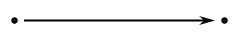
\includegraphics[width=0.8\linewidth]{figures/intro/scg/arcs/const/scg_const_perm_positive2.png}} & \parbox[|c]{2cm}{\centering\ni} & \parbox[|m]{2cm}{\centering\in} & \parbox[|c]{2cm}{\centering->} & \parbox[|m|]{2cm}{\centering<-} \\
	\hline
	
	\parbox[m|]{4.6cm}{\textit{\\ константная постоянная негативная sc-дуга принадлежности \\}} & \parbox[m|]{3.5cm}{\centering 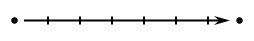
\includegraphics[width=0.8\linewidth]{figures/intro/scg/arcs/const/scg_const_perm_negative2.png}} & \parbox[m]{2cm}{\centering \not\ni} & \parbox[m|]{2cm}{\centering\notin} & \parbox[m|]{2cm}{\centering-|>} & \parbox[m]{2cm}{\centering<|-} \\
	\hline
	
	\parbox[m]{4.6cm}{\textit{\\ константная постоянная нечеткая sc-дуга принадлежности \\}} & \parbox[m]{3.5cm}{\centering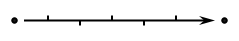
\includegraphics[width=0.8\linewidth]{figures/intro/scg/arcs/const/scg_const_perm_fuzzy2.png}} & \parbox[m]{2cm}{\centering / \ni} & \parbox[m]{2cm}{\centering \in /} & \parbox[m]{2cm}{\centering -/>} & \parbox[m]{2cm}{\centering </-} \\
	\hline
	
	\parbox[m]{4.6cm}{\textit{\\ константная временная позитивная sc-дуга принадлежности \\}} & \parbox[m]{3.5cm}{\centering 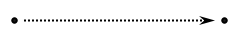
\includegraphics[width=0.8\linewidth]{figures/intro/scg/arcs/const/scg_const_temp_positive2.png}} & \parbox[m]{2cm}{\centering \sim \ni} & \parbox[m]{2cm}{\centering \in \sim} & \parbox[m]{2cm}{\centering \sim>} & \parbox[m]{2cm}{\centering <\sim} \\
	\hline
	
	\parbox[m]{4.6cm}{\textit{\\ константная временная негативная sc-дуга принадлежности \\}} & \parbox[m]{3.5cm}{\centering 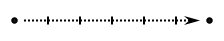
\includegraphics[width=0.8\linewidth]{figures/intro/scg/arcs/const/scg_const_temp_negative2.png}} & \parbox[m]{2cm}{\centering \sim \not\ni} & \parbox[m]{2cm}{\centering \notin \sim} & \parbox[m]{2cm}{\centering \sim|>} & \parbox[m]{2cm}{\centering <|\sim} \\
	\hline
	
	\parbox[m]{4.6cm}{\textit{\\ константная временная нечеткая sc-дуга принадлежности \\}} & \parbox[m]{3.5cm}{\centering 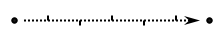
\includegraphics[width=0.8\linewidth]{figures/intro/scg/arcs/const/scg_const_temp_fuzzy2.png}} & \parbox[m]{2cm}{\centering \sim / \ni}  & \parbox[m]{2cm}{\centering \in/\sim} & \parbox[m]{2cm}{\centering \sim/>} & \parbox[m]{2cm}{\centering </\sim} \\
	\hline
	
	\parbox[m]{4.6cm}{\textit{\\ переменная постоянная позитивная sc-дуга принадлежности \\}} & \parbox[m]{3.5cm}{\centering 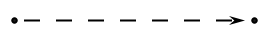
\includegraphics[width=0.8\linewidth]{figures/intro/scg/arcs/var/scg_var_perm_positive2.png}} & \parbox[m]{2cm}{\centering \textunderscore \ni} & \parbox[m]{2cm}{\centering \textunderscore \in} & \parbox[m]{2cm}{\centering \textunderscore->} & \parbox[m]{2cm}{\centering <-\textunderscore} \\
	\hline
	
	\parbox[m]{4.6cm}{\textit{\\ переменная постоянная негативная sc-дуга принадлежности \\}} & \parbox[m]{3.5cm}{\centering 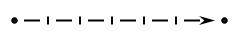
\includegraphics[width=0.8\linewidth]{figures/intro/scg/arcs/var/scg_var_perm_negative2.png}} & \parbox[m]{2cm}{\centering \textunderscore \not\ni} & \parbox[m]{2cm}{\centering \notin \textunderscore} & \parbox[m]{2cm}{\centering \textunderscore-|>} & \parbox[m]{2cm}{\centering <|-\textunderscore} \\
	\hline
	
	\parbox[m]{4.6cm}{\textit{\\ переменная постоянная нечеткая sc-дуга принадлежности \\}} & \parbox[m]{3.5cm}{\centering 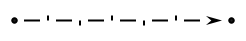
\includegraphics[width=0.8\linewidth]{figures/intro/scg/arcs/var/scg_var_perm_fuzzy2.png}} & \parbox[m]{2cm}{\centering \textunderscore /\ni} & \parbox[m]{2cm}{\centering \in/\textunderscore} & \parbox[m]{2cm}{\centering \textunderscore-/>} & \parbox[m]{2cm}{\centering </-\textunderscore} \\
	\hline
	
	\parbox[m]{4.6cm}{\textit{\\ переменная временная позитивная sc-дуга принадлежности \\}} & \parbox[m]{3.5cm}{\centering 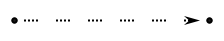
\includegraphics[width=0.8\linewidth]{figures/intro/scg/arcs/var/scg_var_temp_positive2.png}} & \parbox[m]{2cm}{\centering \textunderscore \sim \ni} & \parbox[m]{2cm}{\centering \in \sim \textunderscore} & \parbox[m]{2cm}{\centering \textunderscore \sim >} & \parbox[m]{2cm}{\centering < \sim \textunderscore} \\
	\hline
	
	\parbox[m]{4.6cm}{\textit{\\ переменная временная негативная sc-дуга принадлежности \\}} & \parbox[m]{3.5cm}{\centering 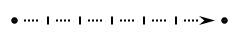
\includegraphics[width=0.8\linewidth]{figures/intro/scg/arcs/var/scg_var_temp_negative2.png}} & \parbox[m]{2cm}{\centering \textunderscore \sim \not$\ni$} & \parbox[c]{2cm}{\centering \notin \sim \textunderscore} & \parbox[m]{2cm}{\centering \textunderscore \sim |>} & \parbox[m]{2cm}{\centering <| \sim \textunderscore} \\
	\hline
	
	\parbox[m]{4.6cm}{\textit{\\переменная временная нечеткая sc-дуга принадлежности\\}} & \parbox[m]{3.5cm}{\centering 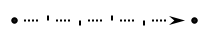
\includegraphics[width=0.8\linewidth]{figures/intro/scg/arcs/var/scg_var_temp_fuzzy2.png}} & \parbox[m]{2cm}{\centering \textunderscore \sim / \ni} & \parbox[m]{2cm}{\centering \in/\sim\textunderscore} & \parbox[m]{2cm}{\centering \textunderscore \sim />} & \parbox[m]{2cm}{\centering </\sim \textunderscore} \\
	\hline
	
	\parbox[m]{4.6cm}{\textit{\\метапеременная постоянная позитивная sc-дуга принадлежности\\}} & \parbox[m]{3.5cm}{\centering 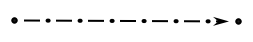
\includegraphics[width=0.8\linewidth]{figures/intro/scg/arcs/meta/scg_metavar_perm_positive2.png}} & \parbox[m]{2cm}{\centering\textunderscore \textunderscore\ni} & \parbox[m]{2cm}{\centering\in\textunderscore\textunderscore} & \parbox[m]{2cm}{\centering\textunderscore\textunderscore->} & \parbox[m]{2cm}{\centering <-\textunderscore\textunderscore} \\
	\hline
	
	\parbox[m]{4.6cm}{\textit{\\ метапеременная постоянная негативная sc-дуга принадлежности \\}} & \parbox[m]{3.5cm}{\centering 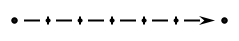
\includegraphics[width=0.8\linewidth]{figures/intro/scg/arcs/meta/scg_metavar_perm_negative2.png}} & \parbox[m]{2cm}{\centering \textunderscore\textunderscore \not\ni} & \parbox[m]{2cm}{\centering \notin\textunderscore\textunderscore} & \parbox[m]{2cm}{\centering \textunderscore\textunderscore-|>} & \parbox[m]{2cm}{\centering <|-\textunderscore\textunderscore} \\
	\hline
	
	\parbox[m]{4.6cm}{\textit{\\ метапеременная постоянная нечеткая sc-дуга принадлежности \\}} & \parbox[m]{3.5cm}{\centering 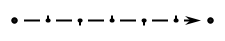
\includegraphics[width=0.8\linewidth]{figures/intro/scg/arcs/meta/scg_metavar_perm_fuzzy2.png}} & \parbox[m]{2cm}{\centering\textunderscore\textunderscore/\ni} & \parbox[m]{2cm}{\centering\in/\textunderscore\textunderscore} & \parbox[m]{2cm}{\centering\textunderscore\textunderscore-/>} & \parbox[m]{2cm}{\centering </-\textunderscore\textunderscore} \\
	\hline
	
	\parbox[m]{4.6cm}{\textit{\\ метапеременная временная позитивная sc-дуга принадлежности \\}} & \parbox[m]{3.5cm}{\centering 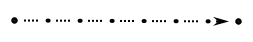
\includegraphics[width=0.8\linewidth]{figures/intro/scg/arcs/meta/scg_metavar_temp_positive2.png}} & \parbox[m]{2cm}{\centering\textunderscore\textunderscore\sim\ni} & \parbox[m]{2cm}{\centering\in\sim\textunderscore\textunderscore} & \parbox[m]{2cm}{\centering\textunderscore\textunderscore\sim>} & \parbox[m]{2cm}{\centering <\sim\textunderscore\textunderscore} \\
	\hline
	
	\parbox[m]{4.6cm}{\textit{\\ метапеременная временная негативная sc-дуга принадлежности \\}} & \parbox[m]{3.5cm}{\centering 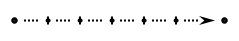
\includegraphics[width=0.8\linewidth]{figures/intro/scg/arcs/meta/scg_metavar_temp_negative2.png}} & \parbox[m]{2cm}{\centering \textunderscore\textunderscore\sim \not\ni} & \parbox[m]{2cm}{\centering\notin\sim\textunderscore\textunderscore} & \parbox[m]{2cm}{\centering\textunderscore\textunderscore\sim|>} & \parbox[m]{2cm}{\centering <|\sim\textunderscore\textunderscore} \\
	\hline
	
	\parbox[m]{4.6cm}{\textit{\\ метапеременная временная нечеткая sc-дуга принадлежности \\}} & \parbox[m]{3.5cm}{\centering 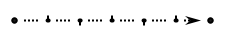
\includegraphics[width=0.8\linewidth]{figures/intro/scg/arcs/meta/scg_metavar_temp_fuzzy2.png}} & \parbox[m]{2cm}{\centering \textunderscore\textunderscore\sim/\ni} & \parbox[m]{2cm}{\centering\in/\sim\textunderscore\textunderscore} & \parbox[m]{2cm}{\centering\textunderscore\textunderscore\sim/>} & \parbox[m]{2cm}{\centering</\sim\textunderscore\textunderscore} \\
	\hline
\end{longtable}
}
%---------------------------------------------
\scnheader{Таблица. Алфавит sc.s-коннекторов, соответствующих sc.g-коннекторам, которые не являются sc.g-дугами принадлежности}
\scneqtable{
\begin{longtable}[l]{|m{6.2cm}|m{2.5cm}|m{2.5cm}|m{2.5cm}|m{2.5cm}|}
	\hline
	\multicolumn{1}{|c}{\parbox[c]{6.2cm}{Изображение \textit{sc-коннектора} в SCg}} &
	\multicolumn{2}{|c}{\parbox[c]{5cm}{Изображение \textit{sc.s-коннектора} в Расширенном алфавите}} &
	\multicolumn{2}{|c|}{\parbox[c]{5cm}{Изображение \textit{sc.s-коннектора} в Базовом алфавите}}
	\hline
	\endhead
	
	\parbox[|c]{6.2cm}{\\\centering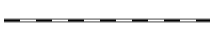
\includegraphics[width=0.8\linewidth]{figures/intro/scs/sc.s-connectors/noorient.png}\\} & \multicolumn{2}{c|}{ \parbox[c]{5cm}{\centering\leftrightarrow}} & \multicolumn{2}{c|}{ \parbox[c]{5cm}{\centering<>}} \\
	\hline
	
	\parbox[c]{6.2cm}{\\\centering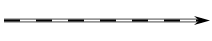
\includegraphics[width=0.8\linewidth]{figures/intro/scs/sc.s-connectors/orient.png} \\} &\parbox[c]{2.5cm}{\\\centering\rightarrow\\} & \parbox[c]{2.5cm}{\\\centering\leftarrow\\} & \parbox[c]{2.5cm}{\\\centering >>\\} & \parbox[c|]{2.5cm}{\\\centering <<\\} \\
	\hline
	
	\parbox[c]{6.2cm}{\\\centering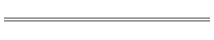
\includegraphics[width=0.8\linewidth]{figures/intro/scs/sc.s-connectors/constPermNoorien.png}\\} & \multicolumn{2}{c|}{\parbox[c]{5cm}{\centering\Leftrightarrow}} & \multicolumn{2}{c|}{\parbox[c]{5cm}{\centering<=>}} \\
	\hline
	
	\parbox[c]{6.2cm}{\\\centering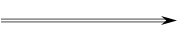
\includegraphics[width=0.8\linewidth]{figures/intro/scs/sc.s-connectors/constPermOrient.png}\\} & \parbox[c]{2.5cm}{\centering\Rightarrow} & \parbox[c]{2.5cm}{\centering\Leftarrow} & \parbox[c]{2.5cm}{\centering =>} & \parbox[c|]{2.5cm}{\centering <=} \\
	\hline
	
	\parbox[c]{6.2cm}{\\\centering
\includegraphics[width=0.8\linewidth]{figures/intro/scs/sc.s-connectors/constTempNoorien.png}\\} & \multicolumn{2}{c|}{\parbox[c]{5cm}{\centering\sim\Leftrightarrow}} & \multicolumn{2}{c|}{\parbox[c|]{5cm}{\centering\sim<=>}} \\
	\hline
	
	\parbox[c]{6.2cm}{\\\centering 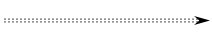
\includegraphics[width=0.8\linewidth]{figures/intro/scs/sc.s-connectors/constTempOrient.png}\\} & \parbox[c]{2.5cm}{\centering\sim\Rightarrow} & \parbox[c]{2.5cm}{\centering\Leftarrow\sim} & \parbox[c]{2.5cm}{\centering\sim=>} & \parbox[c|]{2.5cm}{\centering <=\sim} \\
	\hline
	
	\parbox[c]{6.2cm}{\\\centering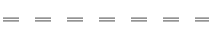
\includegraphics[width=0.8\linewidth]{figures/intro/scs/sc.s-connectors/varPermNoorien.png}\\} & \multicolumn{2}{c|}{\parbox[c]{5cm}{\centering\textunderscore\Leftrightarrow}} & \multicolumn{2}{c|}{\parbox[c|]{5cm}{\centering\textunderscore<=>}} \\
	\hline
	
	\parbox[c]{6.2cm}{\\\centering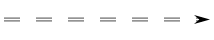
\includegraphics[width=0.8\linewidth]{figures/intro/scs/sc.s-connectors/varPermOrient.png}\\} & \parbox[c]{2.5cm}{\centering\textunderscore\Rightarrow} & \parbox[c]{2.5cm}{\centering\Leftarrow\textunderscore} & \parbox[c]{2.5cm}{\centering\textunderscore=>} & \parbox[c|]{2.5cm}{\centering <=\textunderscore} \\
	\hline
	
	\parbox[c]{6.2cm}{\\\centering
\includegraphics[width=0.8\linewidth]{figures/intro/scs/sc.s-connectors/varTempNoorien.png}\\} & \multicolumn{2}{c|}{\parbox[c]{5cm}{\centering\textunderscore\sim\Leftrightarrow}} & \multicolumn{2}{c|}{\parbox[c]{5cm}{\centering\textunderscore\sim<=>}} \\
	\hline
	
	\parbox[c]{6.2cm}{\\\centering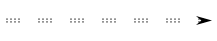
\includegraphics[width=0.8\linewidth]{figures/intro/scs/sc.s-connectors/varTempOrient.png}\\} & \parbox[c]{2.5cm}{\centering\textunderscore\sim\Rightarrow} & \parbox[c]{2.5cm}{\centering\Leftarrow\sim\textunderscore} & \parbox[c]{2.5cm}{\centering\textunderscore\sim=>} & \parbox[c|]{2.5cm}{\centering <=\sim\textunderscore} \\
	\hline
	
	\parbox[c]{6.2cm}{\\\centering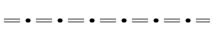
\includegraphics[width=0.8\linewidth]{figures/intro/scs/sc.s-connectors/metaPermNoorien.png}\\} & \multicolumn{2}{c|}{\parbox[c]{5cm}{\centering\textunderscore\textunderscore\Leftrightarrow}} & \multicolumn{2}{c|}{\parbox[c|]{5cm}{\centering\textunderscore\textunderscore<=>}} \\
	\hline
	
	\parbox[c]{6.2cm}{\\\centering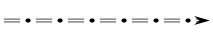
\includegraphics[width=0.8\linewidth]{figures/intro/scs/sc.s-connectors/metaPermOrient.png}\\} & \parbox[c]{2.5cm}{\centering\textunderscore\textunderscore\Rightarrow} & \parbox[c]{2.5cm}{\centering\Leftarrow\textunderscore\textunderscore} & \parbox[c]{2.5cm}{\centering\textunderscore\textunderscore=>} & \parbox[c|]{2.5cm}{\centering <=\textunderscore\textunderscore} \\
	\hline
	
	\parbox[c]{6.2cm}{\\\centering
\includegraphics[width=0.8\linewidth]{figures/intro/scs/sc.s-connectors/metaTempNoorien.png}\\} & \multicolumn{2}{c|}{\parbox[c]{5cm}{\centering\textunderscore\textunderscore\sim\Leftrightarrow}} & \multicolumn{2}{c|}{\parbox[c]{5cm}{\centering\textunderscore\textunderscore\sim<=>}} \\
	\hline
	
	\parbox[c]{6.2cm}{\\\centering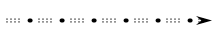
\includegraphics[width=0.8\linewidth]{figures/intro/scs/sc.s-connectors/metaTempOrient.png}\\} & \parbox[c]{2.5cm}{\centering\textunderscore\textunderscore\sim\Rightarrow} & \parbox[c]{2.5cm}{\centering\Leftarrow\sim\textunderscore\textunderscore} & \parbox[c]{2.5cm}{\centering\textunderscore\textunderscore\sim\Rightarrow} & \parbox[c|]{2.5cm}{\centering\Leftarrow\sim\textunderscore\textunderscore} \\
	\hline
	
	\parbox[c]{6.2cm}{\\\centering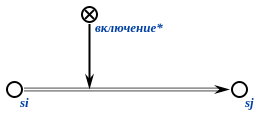
\includegraphics[width=0.8\linewidth]{figures/intro/scs/sc.s-connectors/examples/scs_transf_inclusion_const.png}\\} & \parbox[c]{2.5cm}{\centering\supseteq} & \parbox[c]{2.5cm}{\centering\subseteq} & \multicolumn{2}{c|}{\parbox[c]{5cm}{}} \\
	\hline
	
	\parbox[c]{6.2cm}{\\\centering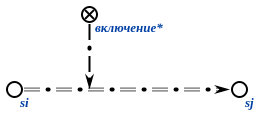
\includegraphics[width=0.8\linewidth]{figures/intro/scs/sc.s-connectors/examples/scs_transf_inclusion_meta.png}\\} & \parbox[c]{2.5cm}{\centering\textunderscore\supseteq} & \parbox[c]{2.5cm}{\centering\subseteq\textunderscore} & \multicolumn{2}{c|}{\parbox[c|]{5cm}{\centering}} \\
	\hline
	
	\parbox[c]{6.2cm}{\\\centering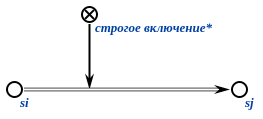
\includegraphics[width=0.8\linewidth]{figures/intro/scs/sc.s-connectors/examples/scs_transf_strict_inclusion_const.png}\\} & \parbox[c]{2.5cm}{\centering\supset} & \parbox[c]{2.5cm}{\centering\subset} & \multicolumn{2}{c|}{\parbox[c|]{5cm}{}} \\
	\hline
	
	\parbox[c]{6.2cm}{\\\centering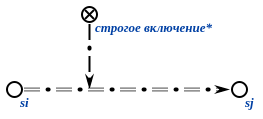
\includegraphics[width=0.8\linewidth]{figures/intro/scs/sc.s-connectors/examples/scs_transf_strict_inclusion_meta.png}\\} & \parbox[c]{2.5cm}{\centering\textunderscore\supset} & \parbox[c]{2.5cm}{\centering\subset\textunderscore} & \multicolumn{2}{c|}{\parbox[c|]{5cm}{}} \\
	\hline
	
	\parbox[c]{6.2cm}{\\\centering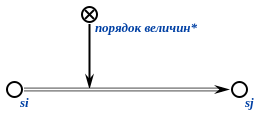
\includegraphics[width=0.8\linewidth]{figures/intro/scs/sc.s-connectors/examples/scs_transf_value_order_const.png}\\} & \parbox[c]{2.5cm}{\centering\geq} & \parbox[c]{2.5cm}{\centering\leq} & \multicolumn{2}{c|}{\parbox[c|]{5cm}{}} \\
	\hline
	
	\parbox[c]{6.2cm}{\\\centering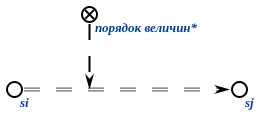
\includegraphics[width=0.8\linewidth]{figures/intro/scs/sc.s-connectors/examples/scs_transf_value_order_var.png}\\} & \parbox[c]{2.5cm}{\centering\textunderscore\geq} & \parbox[c]{2.5cm}{\centering\textunderscore\leq} & \multicolumn{2}{c|}{\parbox[c]{5cm}{}}  \\
	\hline
	
	\parbox[c]{6.2cm}{\\\centering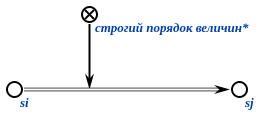
\includegraphics[width=0.8\linewidth]{figures/intro/scs/sc.s-connectors/examples/scs_transf_value_strict_order_const.png}\\} & \parbox[c]{2.5cm}{\centering >} & \parbox[c]{2.5cm}{\centering <} & \multicolumn{2}{c|}{\parbox[c]{5cm}{}} \\
	\hline
	
	\parbox[c]{6.2cm}{\\\centering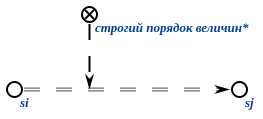
\includegraphics[width=0.8\linewidth]{figures/intro/scs/sc.s-connectors/examples/scs_transf_value_strict_order_var.png}\\} & \parbox[c]{2.5cm}{\centering\textunderscore>} & \parbox[c]{2.5cm}{\centering <\textunderscore} & \multicolumn{2}{c|}{\parbox[c]{5cm}{}} \\
	\hline
	
	\parbox[c]{6.2cm}{\\\centering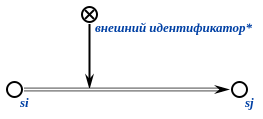
\includegraphics[width=0.8\linewidth]{figures/intro/scs/sc.s-connectors/examples/scs_transf_external_idtf_const.png}\\} & \multicolumn{2}{c|}{\parbox[c]{5cm}{\centering :=}} & \multicolumn{2}{c|}{\parbox[c]{5cm}{}} \\
	\hline
	
	\parbox[c]{6.2cm}{\\\centering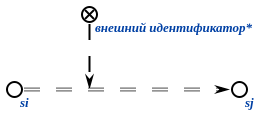
\includegraphics[width=0.8\linewidth]{figures/intro/scs/sc.s-connectors/examples/scs_transf_external_idtf_var.png}\\} & \multicolumn{2}{c|}{\parbox[c]{5cm}{\centering\textunderscore:=}} & \multicolumn{2}{c|}{\parbox[c]{5cm}{}} \\
	\hline
	
	\parbox[c]{6.2cm}{\\\centering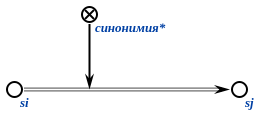
\includegraphics[width=0.8\linewidth]{figures/intro/scs/sc.s-connectors/examples/scs_transf_synonymy_const.png}\\} & \multicolumn{2}{c|}{\parbox[c]{5cm}{\centering =}} & \multicolumn{2}{c|}{\parbox[c]{5cm}{}} \\
	\hline
	
	\parbox[c]{6.2cm}{\\\centering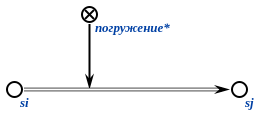
\includegraphics[width=0.8\linewidth]{figures/intro/scs/sc.s-connectors/examples/scs_transf_insertion_const.png}\\} & \parbox[c]{2.5cm}{\centering\supset=} & \parbox[c]{2.5cm}{\centering = \subset} &  \multicolumn{2}{c|}{\parbox[c]{5cm}{}}  \\
	\hline
\end{longtable}
}

\scnendstruct \scninlinesourcecommentpar{Завершили Описание sc.s-разделителей и sc.s-ограничителей}

\scnsegmentheader{Описание sc.s-предложений}
\scnstartsubstruct

\scnheader{sc.s-предложение}
\scnidtf{минимальный семантически целостный фрагмент sc.s-текста}
\scnidtf{минимальный sc.s-текст}
\scnsubset{sc.s-текст}
\scnsuperset{простое sc.s-предложение\\
    \scnaddlevel{1}
    \scnidtf{минимальное sc.s-предложение}
    \scnexplanation{\textit{sc.s-предложение}, (1) \uline{состоящее} или из двух \textit{sc-идентификаторов}, соединенных между собой \textit{sc.s-коннектором}, или из трех \textit{sc-идентификаторов}, разделенных \textit{sc.s-разделителями, изображающими связь инцидентности sc-элементов}, и (2) завершающееся \textit{двойной точкой с запятой}}
    \scnnote{Нетрудно заметить, что простые sc.s-предложения по сути аналогичны триплетам языка RDF (RDF-триплетам), за тем исключением, что \textit{простое sc.s-предложение} можно "развернуть"\ при помощи \textit{Операции конверсии sc.s-предложений*} не меняя при этом его смысл, а RDF-триплет нельзя. Это является одной из причин, по которой, в отличие от RDF-триплетов, в простых sc.s-предложениях \textit{sc.s-коннекторы} и \textit{sc.s-разделители, изображающие связь инцидентности sc-элементов} не могут быть опущены, поскольку они в том числе показывают направление изображаемой ими связи между sc-элементами.}
\scnrelfromlist{пример}{
    \scnfileitem{\textit{многоугольник} $\supset$ \textit{треугольник}}
    \scnaddlevel{1}
    \scnrelboth{семантическая эквивалентность}{\scnfilescg{figures/intro/scs/inclusion.png}}
    \scnaddlevel{-1};
    \scnfileitem{\textit{сторона*} $\ni$ (\textit{Четырехугк(ТчкА\char59ТчкВ\char59ТчкС\char59ТчкD)} $\Rightarrow$ \textit{Отр(ТчкВ\char59ТчкС)})\char59\char59}
    \scnaddlevel{1}
    \scnrelboth{семантическая эквивалентность}{\scnfilescg{figures/intro/scs/side.png}}
    \scnaddlevel{-1};
    \scnfileitem{\textit{Si} |- \textit{ai} >| \textit{ei}}
    \scnaddlevel{1}
    \scnrelboth{семантическая эквивалентность}{\scnfilescg{figures/intro/scs/inclusion_incident.png}}
    \scnaddlevel{-1}
    }
\scnaddlevel{-1}}
\scnnote{Признаком завершения любого \textit{sc.s-предложения}, т.е. последними его символами является \textit{двойная точка с запятой}, которую, следовательно, можно считать разделителем \textit{sc.s-предложений}.}
\scnrelfromlist{заданная операция}{Операция конверсии sc.s-предложения*\\
    \scnaddlevel{1}
    \scnsubset{синтаксическая трансформация*}
    \scnexplanation{Каждое \textit{sc.s-предложение} (в том числе, и \textit{простое sc.s-предложение}) можно преобразовать в семантически эквивалентное ему \textit{sc.s-предложение} путем конверсии ("разворота") цепочки компонентов \textit{sc.s-предложения}. Так, например, при конверсии ("развороте") простого \textit{sc.s-предложения} (1) первый его \textit{sc-идентификатор} (первый компонент этого \textit{sc.s-предложения}) становится третьим компонентом конвертированного\textit{ sc.s-предложения}, (2) второй его \textit{sc-идентификатор} (третий компонент исходного \textit{sc.s-предложения}) становится первым компонентом "конвертированного"\ \textit{sc.s-предложения} и (3) второй компонент исходного \textit{sc.s-предложения} (\textit{sc.s-коннектор} или \textit{sc.s-разделитель, изображающий связь инцидентности sc-элементов}, соединяющий указанные выше компоненты) остается вторым компонентом конвертированного \textit{sc.s-предложения}, но меняет направленность ("$\ni$"\ заменяется на "$\in$"\ и наоборот, "$\supset$"\ на "$\subset$"\ и наоборот, "$\Rightarrow$"\ на "$\Leftarrow$"\ и наоборот и т.д.)}
    \scnnote{Можно говорить не только о конверсии sc.s-предложения, но и о конверсии sc.s-коннектора, о конверсии sc.s-разделителя, изображающего связь инцидентности sc.s-элементов.}
    \scnrelfrom{sc.s-текст до трансформации}{\scnfilelong{\textit{треугольник $\ni$ Треуг(ТчкВ\char59ТчкС\char59ТчкD)}\char59\char59}}
    \scnrelfrom{sc.s-текст после трансформации}{\scnfilelong{\textit{Треуг(ТчкВ\char59ТчкС\char59ТчкD) $\in$ треугольник}\char59\char59}}
	\scnaddlevel{1}
    \scnrelboth{семантическая эквивалентность}{\scnfilescg{figures/intro/scs/conversion.png}}
    \scnaddlevel{-2}
;Операция присоединения sc.s-предложения*\\
    \scnaddlevel{1}
    \scnsubset{синтаксическая трансформация*}
    \scnidtf{Операция соединения двух sc.s-предложений при совпадении последнего компонента первого предложения с первым компонентом второго*}
    \scnexplanation{В результате выполнения данной операции:
    \begin{scnitemize}
        \item первый компонент второго sc.s-предложения удаляется\char59
        \item оставшаяся часть второго предложения окружается sc.s-ограничителем присоединенных предложений ("(*"\ и "*)"). Разделитель sc.s-предложений (";;") также попадает внутрь указанного ограничителя\char59
        \item полученная конструкция помещается между последним компонентом первого предложения и разделителем sc.s-предложений, которым заканчивалось первое предложение\char59
        \item второе предложение, таким образом, становится присоединенным sc.s-предложением.
    \end{scnitemize}
    Аналогичным образом к любому присоединенному sc.s-предложению могут "пристыковываться"\ другие присоединенные sc.s-предложения, в общем случае уровень такой вложенности не ограничен.
    }
    \scnaddlevel{-1}
;Операция слияния sc.s-предложений*\\
    \scnaddlevel{1}
    \scnsubset{синтаксическая трансформация*}
    \scnidtf{Операция присоединения простого sc.s-предложения к sc.s-предложению, у которого последний sc.s-коннектор совпадает с sc.s-коннектором простого sc.s-предложения, а предшествующий указанному sc.s-коннектору sc-идентификатор совпадает с первым sc-идентификатором простого sc.s-предложения*}
    \scnexplanation{В результате выполнения этой операции совпадающие sc-идентификаторы и sc.s-коннекторы соединяемых sc.s-предложений "склеиваются"\ , а последние sc-иден\-ти\-фи\-ка\-то\-ры соединяемых \textit{sc.s-предложений} становятся последними компонентами объединенного \textit{sc.s-предложения},
    разделенными \textit{точкой с запятой}. Аналогичным образом можно присоединять сколько угодно простых \textit{sc.s-предложений}.}
    \scnaddlevel{-1}
;Операция разложения sc.s-предложений на простые sc.s-предложения*\\
    \scnaddlevel{1}
    \scnsubset{синтаксическая трансформация*}
    \scnexplanation{Каждое \textit{sc.s-предложение} можно разложить на множество \textit{простых sc.s-предложений}, т.е. представить в виде последовательности \textit{простых sc.s-предложений}.}
    \scnaddlevel{-1}
;Операция разложения sc.s-предложений на простые sc.s-предложения с sc.s-разделителем, изображающим связь инцидентности sc-элементов*\\
    \scnaddlevel{1}
    \scnsubset{синтаксическая трансформация*}
    \scnexplanation{Каждое \textit{sc.s-предложение} (в том числе и \textit{простое sc.s-предложение} с \textit{sc.s-коннектором}) можно представить в виде семантически эквивалентной последовательности \textit{простых sc.s-предложений} с \textit{sc.s-разделителем, изображающим связь инцидентности sc-элементов}.}
    \scnnote{Данная операция осуществляет \uline{однозначное} (!) формирование множества \textit{простых sc.s-предложений} указанного вида.}
    \scnaddlevel{-1}
    }

\scnheader{sc.s-предложение}
\scnnote{Операции, заданные на множестве \textit{sc.s-предложений} можно разделить на три группы:
    \begin{scnitemize}
        \item группа операций конверсии \textit{sc.s-предложений}, состоящая из одной операции;
        \item группа операций соединения \textit{sc.s-предложений};
        \item группа операций декомпозиции \textit{sc.s-предложений} и, в частности, операций разложения \textit{sc.s-предложений}.
    \end{scnitemize}
Очевидно, что операции соединения \textit{sc.s-предложений} и операции декомпозиции \textit{sc.s-предложений} являются обратными друг другу операциями.}
\scnaddlevel{-1}

\scnheader{Описание примеров выполнения операций, заданных на множестве sc.s-предложений}
\scnstartsubstruct

\bigskip

\scnfilelong{\textit{треугольник $\ni$ Треугк(ТчкВ\char59ТчкС\char59ТчкD)}\char59\char59}
\scnrelfrom{Операция конверсии sc.s-предложения}{\scnfilelong{\textit{Треугк(ТчкВ\char59ТчкС\char59ТчкD) $\in$ треугольник}\char59\char59}}
\scnaddlevel{1}
\scnrelboth{семантическая эквивалентность}{\scnfilescg{figures/intro/scs/conversion.png}}
\scnaddlevel{-1}

\bigskip\bigskip

{\scnfilelong{\textit{треугольник $\ni$ Треугк(ТчкВ\char59ТчкС\char59ТчкD)\char59\char59
\newline
Треугк(ТчкВ\char59ТчкС\char59ТчкD) $\Rightarrow$ сторона*:включение*: Отр(ТчкВ\char59ТчкC)\char59\char59}}}
\scnrelfrom{Операция присоединения sc.s-предложения}{\scnfilelong{\textit{треугольник $\ni$ Треугк(ТчкВ\char59ТчкС\char59ТчкD) (* $\Rightarrow$ сторона*:включение*:Отр(ТчкВ\char59ТчкС)\char59\char59*) }\char59\char59}}
\scnaddlevel{1}
\scnrelboth{семантическая эквивалентность}{\scnfilescg{figures/intro/scs/joining_sentences.png}}
\scnaddlevel{-1}

\bigskip\bigskip

\scnfilelong{\textit{сторона* $\ni$ (Треугк(ТчкВ\char59Тчк С\char59ТчкD) $\Rightarrow$ Отр(ТчкВ\char59ТчкС))\char59\char59
\newline
сторона* $\ni$ (Треугк(ТчкВ\char59Тчк С\char59ТчкD) $\Rightarrow$ Отр(ТчкC\char59ТчкD))\char59\char59}}
\scnrelfrom{Операция слияния sc.s-предложений}{\scnfilelong{\textit{сторона* $\ni$ ((Треугк(ТчкВ\char59ТчкС\char59ТчкD) $\Rightarrow$ Отр(ТчкВ\char59ТчкС))\char59(Треуг(ТчкВ\char59ТчкС\char59ТчкD) $\Rightarrow$ Отр(ТчкC\char59ТчкD)))\char59\char59}}}
\scnaddlevel{1}
\scnrelfrom{синтаксическая трансформация}{\scnfilelong{\textit{Треугк(ТчкВ\char59ТчкС\char59ТчкD)}$\Rightarrow$\textit{сторона*}: \textit{Отр(ТчкВ\char59ТчкС)}\char59\textit{Отр(ТчкС\char59ТчкD)}\char59\char59}}
\scnrelboth{семантическая эквивалентность}{\scnfilescg{figures/intro/scs/joining_sentence.png}}
\scnaddlevel{-1}

\bigskip\bigskip

{\scnfilelong{\textit{Треугк(ТчкВ\char59ТчкС\char59ТчкD) $\Rightarrow$ сторона*:включение*:Отр(ТчкВ\char59ТчкС)\char59\char59}}}
\scnrelfrom{Операция разложения sc.s-предложений на простые sc.s-предложения}{\scnfilelong{\textit{сторона* $\ni$ (Треугк(ТчкВ\char59ТчкС\char59ТчкD) $\Rightarrow$ Отр(ТчкВ\char59ТчкС))\char59\char59
\newline включение* $\ni$ (Треугк(ТчкВ\char59ТчкС\char59ТчкD) $\Rightarrow$ Отр(ТчкВ\char59ТчкС))\char59\char59}}}
\scnaddlevel{1}
\scnrelboth{семантическая эквивалентность}{\scnfilescg{figures/intro/scs/dividing_sentences.png}}
\scnaddlevel{-1}

\bigskip\bigskip

{\scnfilelong{\textit{треугольник $\ni$ Треугк(ТчкВ\char59ТчкC\char59ТчкD)}}}
\scnrelfrom{Операция разложения sc.s-предложений на простые sc.s-предложения с sc.s-разделителем, изображающим связь инцидентности sc-элементов}{\scnfilelong{\textit{треугольник |- ai >| Треугк(ТчкВ\char59ТчкС\char59ТчкD)\char59\char59
\newline
константный постоянный sc-узел, обозначающий класс $\ni$ треугольник\char59\char59
\newline
константная постоянная позитивная sc-дуга принадлежности $\ni$ ai\char59\char59
\newline
константный постоянный sc-узел общего вида $\ni$ Треугк(ТчкВ\char59ТчкC\char59ТчкD)\char59\char59}}}
\scnaddlevel{1}
\scnrelboth{семантическая эквивалентность}{\scnfilescg{figures/intro/scs/dividing_sentences_incident.png}}
\scnaddlevel{-1}

\scnendstruct

\scnheader{присоединенное sc.s-предложение}
\scnidtf{встроенное sc.s-предложение}
\scnexplanation{Присоединенные sc.s-предложения используются для того, чтобы продолжить спецификацию какого-либо sc-элемента, sc-идентификатор которого является последним компонентом в рамках какого-либо sc.s-предложения, не начиная при этом нового sc.s-предложения и, таким образом, не дублируя указанный sc-идентификатор. Внутрь присоединенных sc.s-предложений также могут встраиваться другие присоединенные sc.s-предложения, в общем случае уровень вложенности таких предложений не ограничен. Таким образом присоединенные sc.s-предложения описывают "ветвление"\ sc.s-предложений, при этом точками такого "ветвления"\ выступают sc-идентификаторы, входящие в состав этих sc.s-предложений.

Благодаря введению присоединенных sc.s-предложений появляется возможность любой sc-текст изобразить в виде одного sc.s-предложения, содержащего необходимое количество присоединенных sc.s-предложений. Таким образом, SCs-код по выразительной мощности становится эквивалентным SCn-коду.}

\scnheader{sc.s-предложение}
\scntext{денотационная семантика}{С семантической точки зрения \textit{sc.s-предложение} представляет собой описание некоторого \uline{маршрута} в соответствующем sc-тексте, который является графовой структурой специального вида и структура которого описывается (изображается) с помощью \textit{sc.s-предложений}. Указанный маршрут "проводится"\ по sc-коннекторам и по связям инцидентности sc-элементов, если маршрут проходит через инцидентные sc-коннекторы. В описании указанного маршрута могут дополнительно указываться множества (чаще всего отношения), которым принадлежат sc-коннекторы, входящие в описываемый маршрут. Кроме того, указанный маршрут в начале и/или в конце может иметь разветвления, когда какой-либо sc-элемент \uline{одинаково} инцидентен нескольким \uline{однотипным} sc-коннекторам, соединяющим указанный sc-элемент с некоторыми другими sc-элементами.

Таким образом каждое указанное разветвление состоит из неограниченного числа ветвей, каждая из которых состоит из одного sc-коннектора и одного связываемого им sc-элемента.}

\scnheader{компонент sc.s-предложения*}
\scnexplanation{Каждое \textit{sc.s-предложение} представляет собой последовательность (1) \textit{sc-идентификаторов}, (2) \textit{sc.s-коннекторов} или \textit{sc.s-разделителей}, изображающих связь инцидентности \textit{sc-элементов}, (3) \textit{точек с запятыми}, (4) \textit{ограничителей присоединенных sc.s-предложений}, завершаемая \textit{двойной точкой с запятой}. При этом непосредственно соседствовать друг с другом не могут ни \textit{sc-идентификаторы}, ни \textit{sc.s-коннекторы}, ни, очевидно, \textit{точки с запятыми} и \textit{ограничители присоединенных sc.s-предложений}.\\
Между \textit{sc-идентификаторами} в рамках \textit{sc.s-предложения} может находиться либо \textit{точка с запятой}, либо \textit{sc.s-коннектор}, либо \textit{sc.s-разделитель}, изображающий связь инцидентности \textit{sc-элементов}. Слева и справа от \textit{sc.s-коннектора} и от \textit{sc.s-разделителя}, изображающего связь инцидентности \textit{sc-элементов}, должны находиться \textit{sc-идентификаторы}.

Указанные \textit{sc-идентификаторы}, \textit{sc.s-коннекторы} и \textit{sc.s-разделители}, изображающие связь инцидентности \textit{sc-элементов}, считаются компонентами соответствующего \textit{sc.s-предложения}. Понятие "быть компонентом sc.s-предложения"\ является относительным понятием (отношением), т.к. в состав некоторых компонентов \textit{sc.s-предложения} (в состав \textit{sc-идентификаторов}, являющихся \textit{sc.s-выражениями}, ограничиваемыми фигурными или квадратными скобками) могут входить других \textit{sc.s-предложения}, состоящие из своих компонентов.}
\scnrelfrom{первый домен}{sc.s-предложение}
\scnrelfrom{второй домен}{{\normalfont (} sc-идентификатор $\cup$ sc.s-разделитель $\cup$ sc.s-ограничитель {\normalfont )}}

\scnheader{sc.s-модификатор*}
\scnsubset{компонент sc.s-предложения*}
\scnexplanation{Это дополнительный вид компонентов \textit{sc.s-предложений}. Каждый \textit{sc.s-модификатор}, являющийся компонентом некоторого \textit{sc.s-предложения}, представляет собой \textit{sc-идентификатор}, обозначающий множество (чаще всего, отношение), которому принадлежит sc-коннектор, изображенный \textit{sc.s-коннектором}, который предшествует указанному \textit{sc-идентификатору}. Признаком \textit{sc.s-модификатора} является \textit{двоеточие} (или \textit{двойное двоеточие}), которое ставится после \textit{sc.s-модификатора} и отделяет его либо от следующего за ним другого \textit{sc.s-модификатора} для этого же \textit{sc.s-коннектора}, либо от следующего за ним \textit{sc-идентификатора}, соответствующего sc-элементу, который инцидентен sc-коннектору, изображенному \textit{sc.s-коннектором}, находящимся левее рассматриваемого \textit{sc-идентификатора} после одного или нескольких \textit{sc.s-модификаторов}. Обычное ("одинарное") \textit{двоеточие} обозначает, что sc-элемент, изображенный соответствующим sc.s-модификатором, связан с sc-коннектором, изображенным левее этого sc.s-модификатора, \textit{базовой sc-дугой} (\textit{константной постоянной позитивной sc-дугой принадлежности}), \textit{двойное двоеточие} обозначает, что указанные элементы связаны \textit{переменной постоянной позитивной sc-дугой принадлежности}.}
\scnrelfromlist{пример}{
    \scnfileitem{\textit{Четырехугк(ТчкА;ТчкВ;ТчкС;ТчкD)} $\Rightarrow$ \textit{сторона*} : \textit{включение*} : \textit{Отр(ТчкВ;ТчкС)};; }\\
    \scnaddlevel{1}
    \scnrelboth{семантическая эквивалентность}{\scnfilescg{figures/intro/scs/modifier.png}}
    \scnaddlevel{-1};
    \scnfileitem{\textit{Треугк(ТчкА;ТчкВ;ТчкС)} $\_\Rightarrow$ \textit{сторона*} :: \textit{\_s};; }\\
    \scnaddlevel{1}
    \scnrelboth{семантическая эквивалентность}{\scnfilescg{figures/intro/scs/modifier_var.png}}
    \scnaddlevel{-1}
    }

\scnheader{sc.s-текст}
\scnidtf{конкатенация \textit{sc.s-предложений}}
\scnidtf{последовательность \textit{sc.s-предложений}, разделяемых \textit{двойными точками с запятой}}
\scnsuperset{максимальный исходный sc.s-текст}
    \scnaddlevel{1}
    \scnidtf{конкатенция \textit{sc.s-предложений}, слева и справа от которой отсутствуют какие-либо символы SCs-кода}
    \scnaddlevel{-1}
\scnsuperset{максимальный sc.s-текст, включенный в sc-структуру}
    \scnaddlevel{1}
    \scnidtf{конкатенция всех \textit{sc.s-предложений}, входящих в состав \textit{sc.s-выражения sc-структуры}}
    \scnsuperset{sc.s-текст, включенный в структуру}
        \scnaddlevel{1}
        \scnidtf{часть цепочки \textit{sc.s-предложений}, входящих в состав максимального sc.s-текста, включенного в sc-структуру}
        \scnsuperset{sc.s-предложение, включенное в sc-структуру}
    \scnaddlevel{-2}
\scnnote{\textit{sc.s-предложение} является минимальным sc.s-текстом.}
\scntext{свойство}{Смысл sc.s-текста (а также \textit{sc.s-текста, включенного в sc-структуру} не зависит от порядка \textit{sc.s-предложений} в этих sc-текстах. Т.е. перестановка \textit{sc.s-предложений} в рамках таких sc.s-текстов смысла этих sc.s-текстов не меняет (т.е. приводит к семантически эквивалентным sc.s-текстам), но сильно влияет на трудоемкость человеческого восприятия (на "читабельность") этих текстов.}
\scnrelfrom{пример}{\scnfilelong{
		\textit{материальный объект} $\ni$ \textit{Земля} (* => \textit{вращаться вокруг}*: \textit{спутник}*: \textit{Луна};;*);;\\
		\textit{материальный объект} $\ni$ \textit{Луна}(* => \textit{основной идентификатор}*: [Moon] (* <- \textit{Английский язык};; *); [Луна] (* <- \textit{Русский язык};; *);; *);;\\
		\textit{материальный объект} $\ni$ \textit{Солнце} (* => \textit{вращаться вокруг}*: \textit{Земля}; \textit{Марс};; *);;\\
		\textit{материальный объект} $\ni$ \textit{Марс};;}
}    
\scnaddlevel{1}
\scnrelfrom{семантическая эквивалентность}{ \scnfilescg{figures/intro/scs/scs_text_example.png}}
\scnaddlevel{-1}
    

\newpage

\scnauthorcomment{пересмотреть фрагмент}

\scnheader{sc.s-текст}
\scnidtf{конкатенация \textit{sc.s-предложений}}
\scnidtf{последовательность \textit{sc.s-предложений}, разделяемых \textit{двойными точками с запятой}}
\scnsuperset{максимальный исходный sc.s-текст}
    \scnaddlevel{1}
    \scnidtf{конкатенция \textit{sc.s-предложений}, слева и справа от которой отсутствуют какие-либо символы SCs-кода}
    \scnaddlevel{-1}
\scnsuperset{максимальный sc.s-текст, включенный в sc-структуру}
    \scnaddlevel{1}
    \scnidtf{конкатенция всех \textit{sc.s-предложений}, входящих в состав \textit{sc.s-выражения sc-структуры}}
    \scnaddlevel{-1}
\scnsuperset{исходный sc.s-текст}
    \scnaddlevel{1}
    \scnidtf{часть цепочки \textit{sc.s-предложений}, входящих в состав максимального исходного sc.s-текста}
    \scnsuperset{исходное sc.s-предложение}
    \scnaddlevel{-1}
\scnsuperset{sc.s-текст, включенный в структуру}
    \scnaddlevel{1}
    \scnidtf{часть цепочки \textit{sc.s-предложений}, входящих в состав максимального sc.s-текста, включенного в sc-структуру}
    \scnsuperset{sc.s-предложение, включенное в sc-структуру}
    \scnaddlevel{-1}
\scnnote{\textit{sc.s-предложение} является минимальным sc.s-текстом.}
\scntext{свойство}{Смысл исходного sc.s-текста, а также \textit{sc.s-текста, включенного в sc-структуру} не зависит от порядка \textit{sc.s-предложений} в этих sc-текстах. Т.е. перестановка \textit{sc.s-предложений} в рамках таких sc.s-текстов смысла этих sc.s-текстов не меняет (т.е. приводит к семантически эквивалентным sc.s-текстам), но сильно влияет на трудоемкость человеческого восприятия (на "читабельность") этих текстов.}

\newpage

\scnendstruct \scninlinesourcecommentpar{Завершили Описание sc.s-предложений}

\scnsegmentheader{Описание Ядра SCs-кода и различных направлений его расширения}
\scnstartsubstruct

\scnheader{Ядро SCs-кода}
\scnidtf{Подъязык SCs-кода, который использует минимальный набор синтаксических средств, но при этом имеет семантическую мощность, эквивалентную мощности SCs-кода в целом}
\scntext{принципы, лежащие в основе}{В Ядре SCs-кода:
\begin{scnitemize}
    \item используются только \textit{простые sc-идентификаторы}, в том числе \textit{sc-идентификаторы внешних файлов ostis-систем} (sc-выражения не используются);
    \item используются только \textit{sc.s-разделители, изображающие связь инцидентности sc-элементов}, а также sc.s-коннектор, изображающий константную  постоянную позитивную пару принадлежности ("$\in$" и "$\ni$" в Расширенном алфавите и "{}->{}"\ и "{}<-{}"\ в Базовом алфавите). Другие \textit{sc.s-коннекторы} не используются;
    \item не используются \textit{sc.s-модификаторы} и, соответственно, двоеточия, являющиеся признаком завершения \textit{sc.s-модификаторов};
    \item используются только \textit{простые sc.s-предложения}, которые, как следует из вышеуказанных свойств Ядра SCs-кода, либо состоят из двух \textit{простых sc-идентификаторов}, соединяемых sc.s-коннектором, изображающим константную  постоянную позитивную пару принадлежности, либо трех \textit{простых sc-идентификаторов}, разделенных \textit{sc.s-разделителями, изображающими связь инцидентности sc-элементов}.
\end{scnitemize}

Из перечисленных свойств Ядра SCs-кода следует, что для представления (изображения) любого sc-текста средствами Ядра SCs-кода необходимо для \uline{всех} (!) sc-элементов этого sc-текста (кроме константных постоянных позитивных пар принадлежности) построить соответствующие им простые \textit{sc-идентификаторы}, т.е. необходимо проименовать все указанные sc-элементы. В свою очередь, тип каждого используемого sc-элемента (кроме константных постоянных позитивных пар принадлежности) задается явно путем указания принадлежности этих элементов соответствующим классам sc-элементов, в том числе классам, входящим в Ядро SC-кода.

Как видно из приведенного описания, Ядро SCs-кода соответствует Ядру SCg-кода, за исключением того, что в Ядре SCg-кода нет необходимости именовать все изображаемые sc-элементы, а также в Ядре SCg-кода присутствуют графические изображения для sc-элементов, принадлежащих соответствующим классам Ядра SC-кода и эту принадлежность нет необходимости указывать явно.
}
\scnnote{Очевидно, что широко практически применять Ядро SCs-кода для записи больших фрагментов баз знаний неудобно и неэффективно. Тем не менее, с практической точки зрения Ядро SCs-кода может использоваться, например, для обмена информацией со сторонними средствами представления графовых конструкций, рассчитанными на представление информации в виде триплетов (например, RDF-хранилищ).
Для обеспечения возможности более широкого практического использования необходимы синтаксические расширения Ядра SCs-кода в целях:
\begin{scnitemize}
    \item минимизации числа идентифицируемых (именуемых) sc-элементов путем использования \textit{sc-выражений} и ликвидации необходимости идентифицировать (именовать) \uline{все} (!) sc-элементы;
    \item сокращения текста путем минимизации числа повторений одного и того же \textit{sc-идентификатора} путем соединения \textit{sc.s-предложений};
    \item повышение уровня наглядности, "читабельности"\ sc.s-текстов.
\end{scnitemize}}
\scnhaselementrole{пример}{\scnfilelong{\textit{треугольник |- ai >| Треугк(ТчкВ\char59ТчкС\char59ТчкD)\char59\char59
\newline
Треугк(ТчкВ\char59ТчкС\char59ТчкD) |- bi >| Отр(ТчкВ\char59ТчкС)\char59\char59
\newline
сторона* |- сi >| bi\char59\char59
\newline
константный постоянный sc-узел, обозначающий класс $\ni$ треугольник\char59\char59
\newline
константный постоянный sc-узел, обозначающий отношение $\ni$ сторона*\char59\char59
\newline
константная постоянная позитивная sc-дуга принадлежности $\ni$ ai\char59\char59
\newline
константная постоянная sc-дуга $\ni$ bi\char59\char59
\newline
константная постоянная позитивная sc-дуга принадлежности $\ni$ ci\char59\char59
\newline
константный постоянный sc-узел общего вида $\ni$ Отр(ТчкВ\char59ТчкС)\char59\char59
\newline
константный постоянный sc-узел общего вида $\ni$ Треугк(ТчкВ\char59ТчкC\char59ТчкD)\char59\char59}}}
\scnaddlevel{1}
\scnrelboth{семантическая эквивалентность}{\scnfilescg{figures/intro/scs/kernel_incident.png}}
\scnaddlevel{-1}

\scnheader{Первое направление расширения Ядра SCs-кода}
\scnidtf{Первое направление расширения Ядра SCs-кода \uline{и всех иных его расширений}}
\scntext{принципы}{По сравнению с \textit{Ядром SCs-кода} в \textit{Первом направлении расширения Ядра SCs-кода} вместо \textit{sc-идентификаторов}, являющихся идентификаторами (именами), которые взаимно однозначно соответствуют синонимичным им (представляемым ими) sc-коннекторам, вводятся \textit{sc.s-коннекторы}, каждый из которых соответствует не одному конкретному sc-коннектору, а некоторому классу однотипных sc-коннекторов. Очевидно, что это ликвидирует необходимость \uline{каждому} sc-коннектору приписывать уникальный \textit{sc-идентификатор}. Кроме того, \textit{Алфавит sc.s-коннекторов} включает в себя элементы этого Алфавита (классы \uline{синтаксически} эквивалентных \textit{sc.s-коннекторов}), которые соответствуют \uline{всем} (!) элементам Алфавита sc-коннекторов, но при этом дополнительно включают в себя и другие элементы Алфавита \textit{sc.s-коннекторов}, которые соответствуют часто используемым \uline{семантически} явно выделяемым классам sc-коннекторов. К таким дополнительно вводимым классам \textit{sc.s-коннекторов} относятся \textit{константные sc.s-коннекторы} включения множеств ("$\supset$"\ или "$\subset$"), \textit{переменные sc.s-коннекторы} включения множеств ("$\_\supset$"\ или "$\subset\_$"), \textit{sc.s-коннектор} синонимии ("$=$"), \textit{sc.s-коннектор} погружения ("$=\subset$"\ или "$\supset=$") и др.

Заметим, что указанное расширение Алфавита \textit{sc.s-коннекторов} аналогично расширенному Алфавиту \textit{sc.g-коннекторов} в SCg-коде и ликвидирует необходимость (как и в SCs-коде) явно специфицировать (средствами SCs-кода) синтаксически выделяемые классы \textit{sc.s-коннекторов}.}

\scnheader{Второе направление расширения Ядра SCs-кода}
\scntext{принципы}{Во Втором направлении расширения Ядра SCs-кода вводятся модификаторы \textit{sc.s-коннекторов} (\textit{sc.s-модификаторы}), которые позволяют достаточно компактно дополнительно специфицировать sc-коннекторы, изображаемые (представляемые) соответствующими \textit{sc.s-коннекторами}. Речь идет о такой часто востребованной форме спецификации sc-коннекторов, как указание множества (возможно, нескольких множеств), которому принадлежит специфицируемый  sc-коннектор (чаще всего, таким множеством является \textit{бинарное отношение} (в частности, \textit{ролевое отношение}) или \textit{квазибинарное отношение}).}

\scnheader{sc.s-модификатор*}
\scniselement{отношение}
    \scnaddlevel{1}
    \scnidtf{относительное понятие}
    \scnaddlevel{-1}
\scnidtf{модификатор sc.s-коннектора*}
\scnexplanation{\textit{sc-идентификатор}, который (1) находится либо между \textit{sc.s-коннектором} и \textit{двоеточием}, либо между \textit{двоеточиями} и (2) обозначает множество (чаще всего, отношение), которому принадлежит sc-коннектор, изображаемый ближайшим предшествующим \textit{sc.s-коннектором}. Два подряд идущих двоеточия ("::") обозначают, что указанное множество связано с указанным sc-коннектором \textit{\uline{переменной} позитивной постоянной sc-дугой принадлежности}.

Очевидно, что, если не использовать \textit{sc.s-модификаторы}, указанного вида спецификация sc-коннекторов средствами SCs-кода будет выглядеть значительно более громоздкой.}

\scnheader{Третье направление расширения Ядра SCs-кода}
\scntext{принципы}{В \textit{Третьем направлении расширения Ядра SCs-кода} осуществляется переход от использования только \textit{простых sc-идентификаторов} к использованию как \textit{простых sc-идентификаторов}, так и \textit{sc-выражений}, а также к использованию \textit{sc.s-представлений некоторых неидентифицируемых sc-узлов}. Это существенно сокращает число придумываемых \textit{простых sc-идентификаторов}, т.к. каждое \textit{sc-выражение} в конечном счете — это комбинация \textit{простых sc-идентификаторов}, построенная по правилам, которые достаточно легко семантически интерпретируются. Если проводить аналогию с SCg-кодом, то очевидно, что \textit{sc-выражение}, ограничиваемое фигурными скобками, есть не что иное, как информационная конструкция, ограничиваемая \textit{sc.g-контуром}, а \textit{sc-выражение}, ограничиваемое квадратными скобками есть не что иное, как информационная конструкция, ограничиваемая \textit{sc.g-рамкой}. Отличие здесь заключается в том, что круглыми и квадратными скобками можно ограничивать только линейные информационные конструкции (цепочки символов).}

\scnheader{sc.s-представление неидентифицируемого sc-узла}
\scnidtf{изображение (представление) неидентифицируемого (неименуемого) sc-узла в sc.s-тексте}
\scnidtf{sc.s-обозначение неименуемой сущности, не являющейся парой, обозначаемой sc-коннектором}
\scnidtf{sc.s-представление sc-узла, не являющееся sc-идентификатором (именем этого sc-узла)}
\scnreltoset{разбиение}{sc.s-обозначение неименуемой структуры\\
    \scnaddlevel{1}
    \scnidtf{конкатенация левой фигурной скобки и правой фигурной скобки}
    \scnaddlevel{-1}
;sc.s-обозначение неименуемой неориентированной связки\\
    \scnaddlevel{1}
    \scnidtf{конкатенация левой фигурной скобки, дефиса и правой фигурной скобки}
    \scnaddlevel{-1}
;sc.s-обозначение неименуемого кортежа\\
    \scnaddlevel{1}
    \scnidtf{конкатенация левой угловой скобки, дефиса и правой угловой скобки}
    \scnaddlevel{-1}
;sc.s-обозначение неименуемого файла-экземпляра\\
    \scnaddlevel{1}
    \scnidtf{конкатенация левой квадратной скобки и правой квадратной скобки}
    \scnaddlevel{-1}
;sc.s-обозначение неименуемого файла-класса\\
    \scnaddlevel{1}
    \scnidtf{конкатенация восклицательного знака, левой квадратной скобки и правой квадратной скобки}
    \scnaddlevel{-1}
;sc.s-обозначение неименуемой терминальной сущности\\
    \scnaddlevel{1}
    \scnidtf{конкатенация левой круглой скобки, буквы "о"\ и правой круглой скобки}
    \scnaddlevel{-1}}
\scntext{примечание}{Если одно и то же обозначение неименуемой сущности встречается в \uline{разных} \textit{sc.s-предложениях}, то считается, что это обозначения \uline{разных} сущностей, т.е. изображения \uline{разных} sc-узлов.}

\scnheader{Четвертое направление расширения Ядра SCs-кода}
\scntext{принципы}{В \textit{Четвертом направлении расширения Ядра SCs-кода} осуществляется переход от использования только \textit{простых sc.s-предложений} к использованию также \textit{sc.s-предложений}, построенных с помощью \textit{Операции присоединения sc.s-предложения*}. В результате этого, благодаря "склеиванию"\ одинаковых \textit{sc-идентификаторов}, а также "склеиванию"\ синтаксически эквивалентных \textit{sc.s-коннекторов} с одинаковыми \textit{sc.s-модификаторами} (несмотря на то, что эти "склеиваемые"\ \textit{sc.s-коннекторы} соответствуют \uline{разным} sc-коннекторам), существенно сокращается число копий используемых \textit{sc-идентификаторов} и \textit{sc.s-коннекторов} с их \textit{sc.s-модификаторами}.}

\scnheader{Пятое направление расширения Ядра SCs-кода}
\scntext{принципы}{В \textit{Пятом направлении расширения Ядра SCs-кода} разрешается использование \textit{присоединенных sc.s-предложений}. В результате этого \textit{sc.s-тексты} становятся более компактными и удобными для восприятия за счет снижения числа дублируемых \textit{sc-идентификаторов} и более широких возможностей их структуризации.}

\scnendstruct \scninlinesourcecommentpar{Завершили \textit{Описание Ядра SCs-кода и различных направлений его расширения}}

\scnsegmentheader{Итоговый сегмент введения в SCs-код}
\scnstartsubstruct

\scnheader{следует отличать*}
\scnhaselementset{sc.s-представление неидентифицируемого sc-узла;sc.s-коннектор\\
    \scnaddlevel{1}
    \scnidtf{sc.s-представление неидентифицируемого sc-коннектора}
    \scnaddlevel{-1}}\bigskip
\scnhaselementset{sc-коннектор;sc.s-коннектор}\bigskip
\scnhaselementset{sc.s-коннектор;sc.s-модификатор*\\
    \scnaddlevel{1}
    \scnidtf{модификатор sc.s-коннектора*}
    \scniselement{отношение}
    \scnaddlevel{-1}}\bigskip
\scnhaselementset{sc.s-коннектор;Правила построения sc.s-коннекторов}\bigskip
\scnhaselementset{sc.s-предложение;Правила построения sc.s-предложений}\bigskip
\scnhaselementset{sc.s-коннектор;sc.g-коннектор}\bigskip
\scnhaselementset{sc.s-текст;sc.g-текст}

\scnheader{Примеры sc.s-текстов, трансформируемых по различным направлениям расширений SCs-кода}
\begin{scneqtoset}
    \scnfileitem{\textit{включение* $\ni$ pair1;;\\включение* $\ni$ pair2;;\\включение* $\ni$ pair3;;\\включение* $\ni$ pair4;;\\включение* $\ni$ pair5;;\\сторона* $\ni$ pair1;;\\сторона* $\ni$ pair2;;\\сторона* $\ni$ pair3;;\\сторона* $\ni$ pair4;;\\сторона* $\ni$ pair5;;\\Четырехугк(ТчкА;ТчкВ;ТчкС;ТчкD) |- pair1 >| Отр(ТчкВ;ТчкС);;\\Четырехугк(ТчкА;ТчкВ;ТчкС;ТчкD) |- pair2 >| Отр(ТчкC;ТчкD);;\\Треугк(ТчкВ;ТчкС;ТчкD) |- pair3 >| Отр(ТчкВ;ТчкС);;\\Треугк(ТчкВ;ТчкС;ТчкD) |- pair4 >| Отр(ТчкC;ТчкD);;\\Треугк(ТчкВ;ТчкС;ТчкD) |- pair5 >| Отр(ТчкB;ТчкD);;\\четырехугольник $\ni$ Четырехугк(ТчкА;ТчкВ;ТчкС;ТчкD);;\\треугольник $\ni$ Треугк(ТчкВ;ТчкС;ТчкD);;\\link1 |- pair6 >| Треугк(ТчкВ;ТчкС;ТчкD);;\\декомпозиция фигуры* $\ni$ pair6;;\\link1 $\ni$ Отр(ТчкВ;ТчкС);;\\link1 $\ni$ Отр(ТчкC;ТчкD);;\\link1 $\ni$ Отр(ТчкВ;ТчкD);;}}
    \begin{scnindent}
        \scnrelboth{семантическая эквивалентность}{\scnfileimage[20em]{Contents/part_kb/images/scs/scs_transf_example.png}}
        \scnrelfrom{синтаксическая трансформация}{\scnfilelong{\textit{сторона* $\ni$ (Четырехугк(ТчкА;ТчкВ;ТчкС;ТчкD) $\Rightarrow$ Отр(ТчкВ;ТчкС));;\\сторона* $\ni$ (Четырехугк(ТчкА;ТчкВ;ТчкС;ТчкD) $\supseteq$ Отр(ТчкC;ТчкD));;\\сторона* $\ni$ (Треугк(ТчкВ;ТчкС;ТчкD) $\supseteq$ Отр(ТчкВ;ТчкС));;\\сторона* $\ni$ (Треугк(ТчкВ;ТчкС;ТчкD) $\supseteq$ Отр(ТчкC;ТчкD));;\\сторона* $\ni$ (Треугк(ТчкВ;ТчкС;ТчкD) $\supseteq$ Отр(ТчкB;ТчкD));;\\Четырехугк(ТчкА;ТчкВ;ТчкС;ТчкD) $\supseteq$ Отр(ТчкВ;ТчкС);;\\Четырехугк(ТчкА;ТчкВ;ТчкС;ТчкD) $\supseteq$ Отр(ТчкC;ТчкD);;\\Треугк(ТчкВ;ТчкС;ТчкD) $\supseteq$ Отр(ТчкВ;ТчкС);;\\Треугк(ТчкВ;ТчкС;ТчкD) $\supseteq$ Отр(ТчкC;ТчкD);;\\Треугк(ТчкВ;ТчкС;ТчкD) $\supseteq$ Отр(ТчкB;ТчкD);;\\четырехугольник $\ni$ Четырехугк(ТчкА;ТчкВ;ТчкС;ТчкD);;\\треугольник $\ni$ Треугк(ТчкВ;ТчкС;ТчкD);;\\декомпозиция фигуры* $\ni$ (link1 $\Rightarrow$ Треугк(ТчкВ;ТчкС;ТчкD));;\\link1 $\ni$ Отр(ТчкВ;ТчкС);;\\link1 $\ni$ Отр(ТчкC;ТчкD);;\\link1 $\ni$ Отр(ТчкВ;ТчкD);;}}}
        \begin{scnindent}
            \scnrelfrom{синтаксическая трансформация}{\scnfilelong{\textit{Четырехугк(ТчкА;ТчкВ;ТчкС;ТчкD) $\supseteq$ сторона*: Отр(ТчкВ;ТчкС);;\\Четырехугк(ТчкА;ТчкВ;ТчкС;ТчкD) $\supseteq$ сторона*: Отр(ТчкC;ТчкD);;\\Треугк(ТчкВ;ТчкС;ТчкD) $\supseteq$ сторона*: Отр(ТчкВ;ТчкС);;\\Треугк(ТчкВ;ТчкС;ТчкD) $\supseteq$ сторона*: Отр(ТчкC;ТчкD);;\\Треугк(ТчкВ;ТчкС;ТчкD) $\supseteq$ сторона*: Отр(ТчкB;ТчкD);;\\четырехугольник $\ni$ Четырехугк(ТчкА;ТчкВ;ТчкС;ТчкD);;\\треугольник $\ni$ Треугк(ТчкВ;ТчкС;ТчкD);;\\link1 $\Rightarrow$декомпозиция фигуры*: Треугк(ТчкВ;ТчкС;ТчкD);;\\link1 $\ni$ Отр(ТчкВ;ТчкС);;\\link1 $\ni$ Отр(ТчкC;ТчкD);;\\link1 $\ni$ Отр(ТчкВ;ТчкD);;}}}
            \begin{scnindent}
                \scnrelfrom{синтаксическая трансформация}{\scnfilelong{\textit{Четырехугк(ТчкА;ТчкВ;ТчкС;ТчкD) $\supseteq$ сторона*: Отр(ТчкВ;ТчкС); Отр(ТчкC;ТчкD);;\\Треугк(ТчкВ;ТчкС;ТчкD) $\supseteq$ сторона*: Отр(ТчкВ;ТчкС); Отр(ТчкC;ТчкD); Отр(ТчкB;ТчкD);;\\четырехугольник $\ni$ Четырехугк(ТчкА;ТчкВ;ТчкС;ТчкD);;\\треугольник $\ni$ Треугк(ТчкВ;ТчкС;ТчкD);;\\link1 $\Rightarrow$декомпозиция фигуры*: Треугк(ТчкВ;ТчкС;ТчкD);;\\link1 $\ni$ Отр(ТчкВ;ТчкС); Отр(ТчкC;ТчкD); Отр(ТчкВ;ТчкD);;}}}
                \begin{scnindent}
                    \scnrelfrom{синтаксическая трансформация}{\scnfilelong{\textit{четырехугольник $\ni$ Четырехугк(ТчкА;ТчкВ;ТчкС;ТчкD)(* $\supseteq$ сторона*: Отр(ТчкВ;ТчкС); Отр(ТчкC;ТчкD);; *);;\\треугольник $\ni$ Треугк(ТчкВ;ТчкС;ТчкD)(* $\supseteq$ сторона*: Отр(ТчкВ;ТчкС); Отр(ТчкC;ТчкD); Отр(ТчкB;ТчкD);; *);;\\Треугк(ТчкВ;ТчкС;ТчкD) $\Leftarrow$декомпозиция фигуры*: link1(* $\ni$ Отр(ТчкВ;ТчкС); Отр(ТчкC;ТчкD); Отр(ТчкВ;ТчкD);; *);;}}}
                \end{scnindent}
            \end{scnindent}
        \end{scnindent}
    \end{scnindent}
\end{scneqtoset}

\scnendstruct \scninlinesourcecommentpar{Завершили ``Итоговый сегмент введения в SCs-код''}

\scnendstruct \scninlinesourcecommentpar{Завершили Раздел \ref{intro_scs} ``\nameref{intro_scs}''}

%END SCs

\end{SCn}
\scsubsection{Описание языка структурированного представления знаний ostis-систем}
\label{intro_scn}

\begin{SCn}

\bigskip

\scnsectionheader{\currentname}

\scnstartsubstruct

\scnheader{SCn-код}
\scnidtf{Язык структурированного представления знаний \textit{ostis-систем}}
\scnexplanation{\textit{SCn-код} является языком структурированного внешнего представления текстов \textit{SC-кода} и представляет собой синтаксическое расширение \textit{SCs-кода}, направленное на повышение наглядности и компактности текстов \textit{SCs-кода}. 
	
SCn-код позволяет перейти от линейных текстов \uline{SCs-кода} к форматированным и фактически двухмерным текстам, в которых появляется декомпозиция исходного линейного текста \uline{SCs-кода} на \uline{строчки}, размещенные "по вертикали". При этом начало всех \uline{строчек} текста фиксировано и определяется известным и ограниченным набором правил, что дает возможность использовать это при форматировании \uline{sc.n-текста} (текста, принадлежащего SCn-коду.}
\scniselement{язык двухмерных текстов}
\scnaddlevel{1}
\scnidtf{язык, каждый \textit{текст} которого задается (1) множеством входящих в него \textit{символов}, (2) отношением порядка (последовательности) \textit{символов} по "горизонтали"{}, (3) отношением порядка(последовательности) \textit{символов} по "вертикали".}
\scnaddlevel{1}
\scnexplanation{Символ, входящий в состав \textit{двухмерного текста}, в общем случае может иметь четыре "соседних"{}\textit{символа}: (1) \textit{символ}, находящийся от него \uline{слева} в рамках той же \textit{строчки}, (2) \textit{символ}, находящийся от него \uline{справа} в рамках этой же \textit{строчки}, (3) \textit{символ}, находящийся строго \uline{над} ним в предыдущей \textit{строчке} и (4) \textit{символ}, находящийся строго \uline{под ним} в следующей \textit{строчке} текста.}
\scnaddlevel{-1}
\scnaddlevel{-1}
\scntext{сравнительный анализ}{Благодаря тому, что в состав sc.n-текстов могут входить и sc.s-тексты, и sc.g-тексты (ограниченные sc.n-контуром), SCn-код можно считать интегратором различных внешних языков представления знаний.  Это дает возможность при визуализации и разработке базы знаний ostis-системы недостатки одного из предлагаемых вариантов внешнего представления sc-текстов (SCg-кода, SCs-кода, SCn-кода) компенсировать достоинствами других вариантов.}

\bigskip

\scnmakeset{SCn-код;SCs-код}
\scnrelfrom{описание связи}{\scnstartsetlocal\\
\scnheaderlocal{SCn-код}
\scnrelfrom{синтаксическое расширение;синтаксическое ядро языка}{SCs-код}
\scnendstruct
}
\scntext{отличие}{Переход от линейности sc.s-текстов к двухмерности sc.n-текстов.}
\scnaddlevel{1}
    \scntext{уточнение}{Важной особенностью SCn-кода является "двухмерный"{} характер его текстов. Это проявляется в том, что для каждого фрагмента текста SCn-кода важное значение имеет величина отступа от левого края \textit{строчки}.
    
    В тексте \textit{SCn-кода} в отличие от текста \textit{SCs-кода} для каждого фрагмента текста важное значение имеет не только то, как этот фрагмент связан с другими фрагментами "по горизонтали"{}(какой фрагмент находится \uline{левее} и какой \uline{правее} на одной и той же \textit{строчке}), но и то, как он связан с другими фрагментами "по вертикали"{}(какой фрагмент находится \uline{выше} на предыдущей \textit{строчке} и какой находится \uline{ниже} на следующей \textit{строчке}). Так, например, если в тексте \textit{SCn-кода} некоторый \textit{sc-идентификатор}(внешний идентификатор \textit{sc-элемента}) размещен сразу после вертикальной табуляционной линии и точно \uline{под ним} размещен некоторый \textit{sc.s-коннектор}, то это означает, что указанный \textit{sc-элемент} инцидентен \textit{sc-коннектору}, изображенному указанным \textit{sc.s-коннектором}.
    
    Для того, чтобы обеспечить точное задание(формулировку) правил двухмерной инцидентности элементов(элементарных фрагментов) sc.n-текстов, вводится понятие \textit{\textbf{страницы} sc.n-текста}, понятие \textit{\textbf{строчки} sc.n-текста}, а также используется специальная \uline{разметка}, представляющая собой вертикальные табуляционные линии, расстояние между которыми примерно равняется максимальной длине sc.s-коннектора (обычно это расстояние равно ширине 4-5 символов).}
\scnaddlevel{-1}

\scnheader{sc.n-текст}
\scnidtf{текст SCn-кода}
\scnidtf{последовательность предложений SCn-кода}
\scnidtf{последовательность предложений SCn-кода, каждое из которых не является частью какого-либо другого предложения из \uline{этой} последовательности}

\scnheader{страница sc.n-текста}
\scnidtf{страница, на которой размещается sc.n-текст}
\scnnote{если sc.n-текст является частью какого-либо другого файла, разделяемого на страницы, например, публикации какой-либо части базы знаний, то sc.n-страницей считается только часть страницы, на которой изображен sc.n-текст, в то время как страница указанного файла может быть больше за счет, например, белых полей по краям страницы, необходимых для последующей распечатки.}

\scnheader{строчка sc.n-текста}
\scnnote{Максимальное количество символов в строчках sc.n-текста для каждого sc.n-текста фиксировано и определяется конкретным вариантом размещения sc.n-текста. При этом, в зависимости от отступов в рамках конкретного sc.n-предложения, строчка sc.n-текста может начинаться не с левого края sc.n-текста (но всегда с какой-то из вертикальных линий разметки) и иметь произвольную длину, ограничиваемую правой границей sc.n-страницы.}

\scnheader{линия разметки sc.n-текста}
\scnidtf{табуляционная линия sc.n-текста}
\scnidtf{вертикальная линия разметки sc.n-текста}
\scnidtf{вертикальная табуляционная линия}
\scnidtf{вертикальная линия, используемая для упрощения восприятия sc.n-текстов и показывающая уровень отступа для компонентов sc.n-предложений}
\scnexplanation{1-я линия разметки ограничивает левый край sc.n-страницы, 2-я линия разметки располагается примерно между 5 и 6 символами строчки и т.д. Расстояние между линиями разметки может меняться в зависимости от размера шрифта, однако в рамках одного sc.n-текста всегда остается одинаковым. Общее количество линий разметки ограничивается максимально возможной шириной sc.n-страницы в конкретном файле ostis-системы, содержащем данный sc.n-текст.}

\scnheader{следует отличать*}
\scnhaselementset{страница sc.n-текста;строчка sc.n-текста;строка}

\bigskip

\scnmakeset{SCn-код;SCs-код}
\scnrelfrom{сходство}{\scnstartsetlocal\\
\scnheaderlocal{Алфавит SCs-кода}
\scnreltolist{алфавит}{SCs-код;SCn-код}
\scnendstruct
}
\scnaddlevel{1}
	\scnrelboth{семантически эквивалентная информационная конструкция}			{\scnfilelong{Алфавит символов \textit{SCs-кода} является также алфавитом символов и \textit{SCn-кода}, т.е. \textit{алфавиты}* этих языков совпадают.}}
\scnaddlevel{-1}
\scntext{сходство}{Все компоненты sc.s-текстов используются также и в sc.n-текстах:
\begin{scnitemize}
\item sc-идентификаторы
\item sc.s-коннекторы
\item модификаторы sc.s-коннекторов с соответствующими разделителями (двоеточиями)
\item разделители, используемые в sc-выражениях, обозначающих sc-множества, заданные перечислением элементов с соответствующими разделителями (\textit{точкой с запятой} или \textit{круглым маркером})
\item \textit{круглые маркеры} в перечислениях идентификаторов sc-элементов, связанных однотипными sc-коннекторами с однотипными модификаторами с заданным sc-элементом
\item разделители предложений (двойные точки с запятой) (опускаются при преобразовании sc.s-предложений в sc.n-предложения)
\item ограничители присоединенных sc.s-предложений (опускаются при преобразовании sc.s-предложений в sc.n-предложения)
\end{scnitemize}
}
\scntext{отличие}{В отличие от sc.s-текстов в sc.n-текстах:
\begin{scnitemize}
\item добавляются новые виды sc-выражений (а именно -- sc-выражений, имеющих двухмерный характер);
\item добавляется новый вид разделителей предложений -- пустая строчка;
\item меняется размещение предложений с учетом двухмерного характера такого размещения.
\end{scnitemize}
}
\scntext{отличие}{В \textit{SCn-коде} по сравнению с \textit{SCs-кодом} добавляются новые виды \textit{sc-выражений}:
\begin{scnitemize}
\item \textit{sc-выражение}, представляющее собой двухмерный \textit{sc.n-текст}, ограниченный \textit{sc.n-контуром} или \textit{sc.n-рамкой}. Каждый \textit{sc.n-контур} изображается условно в виде \textit{открывающей фигурной скобки} и расположенной строго \uline{под} ней через несколько строчек \textit{закрывающей фигурной скобки}. Внутри указанных скобок (начиная от линии вертикальной разметки, на которой расположены сами скобки, и до правого края \textit{страницы}) размещается sc.n-текст. Полученный sc.n-контур является изображением sc-структуры, являющейся результатом трансляции указанного sc.n-текста в SC-код. Каждая \textit{sc.n-рамка} изображается аналогичным образом, только вместо \textit{фигурных скобок} в ней используются \textit{квадратные скобки}, либо \textit{квадратные скобки} с \textit{восклицательным знаком} (в случае файла-образца);
\item \textit{sc-выражение}, представляющее собой двухмерный \textit{sc.g-текст}, ограниченный \textit{sc.n-контуром} или \textit{sc.n-рамкой}.
\item \textit{sc-выражение}, представляющее собой ограниченное \textit{sc.n-рамкой} двухмерное графическое изображение \textit{информационной конструкции}, закодированной в некотором \textit{файле ostis-системы}. Такой \textit{информационной конструкцией} может быть таблица, рисунок, фотография, диаграмма, график и многое другое.
\end{scnitemize}
}
\scnaddlevel{1}
	\scnnote{Нетрудно заметить, что \textit{sc.n-контур} является, по сути, двухмерным эквивалентом \textit{sc-выражения sc-структуры}, а \textit{sc.n-рамка} -- двухмерным эквивалентом \textit{sc-выражения внутреннего файла ostis-системы} или \textit{sc-выражения, обозначающего файл-образец ostis-системы}.}
\scnaddlevel{-1}

\scnheader{sc.n-рамка}
\scnidtf{ограничитель изображения файла \uline{ostis-системы}, используемый в \uline{sc.n-предложениях}}

\scnhaselementrole{пример}{\scnsourcecomment{начало sc.n-рамки}\vspace{\baselineskip}\scnfileimage{\bigskip}
	\scnsourcecommentpar{конец sc.n-рамки}}
\scnnote{С формальной точки зрения \textit{sc.n-рамка} всегда представляет собой \uline{одну} \textit{строчку sc.n-текста}. Это означает, что \textit{sc.n-рамка} не может быть синтаксически разделена на части в рамках того \textit{sc.n-текста}, в котором она используется, и внутрь нее не могут вставляться, например, \textit{присоединенные sc.n-предложения} или какой-либо другой текст (за исключением случаев, когда \textit{sc.n-рамка} содержит \textit{sc.n-текст}, но в этом случае указанный \textit{sc.n-текст} все равно будет рассматриваться как целостный внешний файл, а не как фрагмент окружающего его \textit{sc.n-текста}).}

\scnheader{sc.n-контур}
\scnidtf{используемый в \uline{sc.n-предложениях} ограничитель, являющийся изображением sc-структуры}
\scnhaselementrole{пример}{\scnsourcecomment{начало sc.n-контура}\\\settab\scnstartsetlocal \bigskip\\ \scnendstruct \scnsourcecommentpar{конец sc.n-контура}}

\bigskip

\scnmakeset{sc.s-предложение;sc.n-предложение}
\scntext{сходство}{Понятие \textit{sc.n-предложения} является естественным обобщением понятия \textit{sc.s-предложения}. Более того, \uline{аналогичным} для \textit{sc.s-предложений} образом вводятся понятия:
\begin{scnitemize}
%\item \textit{тривиального sc.n-предложения}
\item \textit{простого sc.n-предложения}
\item \textit{сложного sc.n-предложения}
\item \textit{sc.n-предложения, содержащего присоединенные sc.n-предложения}
\item \textit{sc.n-предложения, не содержащего присоединенные sc.n-предложения}
\item \textit{присоединенного sc.n-предложения}
\item \textit{неприсоединенного sc.n-предложения}
\end{scnitemize}}
\filemodetrue
\scnrelfromlist{отличие}{\uline{Если} каждое \textit{неприсоединенное sc.s-предложение} \uline{либо} являетcя первым предложением \textit{sc.s-текста}, \uline{либо} начинается после \textit{разделителя sc.s-предложений} (\textit{двойной точки с запятой}), \uline{то} каждое \textit{неприсоединенное sc.n-предложение} начинается с начала новой строчки;
\uline{Если} каждое \textit{присоединенное sc.s-предложение} начинается либо после открывающего ограничителя присоединенных sc.s-предложений (открывающей круглой скобки со звездочкой), \uline{либо} после \textit{разделителя sc.s-предложений}, \uline{то} каждое \textit{присоединенное sc.n-предложение} начинается с новой строчки под sc-идентификатором, которым завершается то sc.n-предложение (и соответственно, sc.s-предложение), в которое встраивается данное \textit{присоединенное sc.n-предложение}; 
Первый \textit{sc-идентификатор}, входящий в состав \textit{sc.n-предложения} до \textit{sc.s-коннектора} выделяется \uline{жирным} курсивом;
В \textit{sc.n-предложениях двойная точка с запятой} не используется в качестве признака завершения этих предложений и, соответственно, не используется в качестве разделителя \textit{sc.n-предложений}. Таким разделителем является \textit{пустая строчка}.}

\scntext{отличие}{Благодаря двухмерности SCn-кода появляются более широкие возможности (степени свободы) для наглядного и компактного размещения sc.n-предложений.}
\scnaddlevel{1}
\scnrelfromlist{уточнение}{При оформлении sc.n-предложения осуществляется четкая \uline{табуляция} всех присоединенных к нему sc.n-предложений, присоединяемых к исходному "по вертикали". Вертикальная линия табуляции задает левую границу исходного (максимального) sc.n-предложения или левую границу присоединенного sc.n-предложения, присоединяемого "по вертикали". Левая граница sc.n-предложения задает начало первого sc-идентификатора, входящего в состав этого sc.n-предложения, а также начало sc.s-коннектора, инцидентного указанному sc-идентификатору и размещаемого \uline{строго под} этим sc-идентификатором. Расстояние между вертикальными табуляционными линиями фиксировано и примерно равно максимальной длине sc.s-коннектора;
В отличие от sc.s-текстов: в sc.n-текстах sc.s-коннектор может быть инцидентен предшествующему sc-идентификатору (как простому, так и sc-выражению) не только "по горизонтали"{}, но и "по вертикали". Для этого sc.s-коннектор размещается строго \uline{под} предшествующим ему sc-идентификатором;
Кроме того "по вертикали"\ sc-идентификатор может быть инцидентен не одному, а \uline{нескольким} sc.s-коннекторам, которые последовательно "по вертикали"\ размещаются \uline{под} указанным sc-идентификатором. Это позволяет в рамках одного sc.n-предложения представлять произвольное число "ответвлений"\ от каждого sc-идентификатора, т.е. произвольное число sc.s-коннекторов, инцидентных этому sc-идентификатору;
Каждый sc-идентификатор, включая sc-выражение, ограничиваемого фигурными или квадратными скобками, должен размещаться сразу правее вертикальной разметочной линии, если \uline{под ним} размещается sc.s-коннектор;
Каждый sc.s-коннектор выделяется жирным некурсивным шрифтом и, если он находится \uline{под} инцидентным ему sc-идентификатором, размещается строго между двумя вертикальными разметочными линиями, прижимаясь при этом к левой из этих двух разметочных линий.}
\scnaddlevel{-1}
\filemodefalse

\scnheader{SCn-код}
\scntext{правило синтаксической трансформации}{Поскольку по отношению к SCn-коду SCs-код является \textit{синтаксическим ядром языка*}, SCn-код можно рассматривать как результат интеграции нескольких направлений расширения SCs-кода, в основе которых лежат правила синтаксической трансформации sc.s-текстов и sc.n-текстов, ориентированные на повышение эффективности использования тех возможностей обеспечения наглядности и компактности sc.n-текстов, которые открываются при переходе от линейности sc.s-текстов к двухмерности sc.g-текстов}

\scnheader{sc.n-предложение}
\scnrelfromlist{заданная операция}{Операция преобразования sc.s-предложения в sc.n-предложение*\\
	\scnaddlevel{1}
	\scnsubset{синтаксическая трансформация*}
	\scnexplanation{Каждое \textit{sc.s-предложение}, записываемое линейно ("горизонтально") может быть преобразовано в соответствующее двухмерное \textit{sc.n-предложение}. 
	Перечислим основные правила трансформации sc.s-предложений в sc.n-предложения:
	\begin{scnitemize}
		\item sc.s-коннектор может размещаться на следующей строчке под предшествующим sc-идентификатором, начиная с того же символа следующей строчки, что и указанный sc-идентификатор\char59
		\item если sc-идентификатор переносится на следующую строчку, то его продолжение на следующей строчке осуществляется с таким же отступом от начала строчки, с каким указанный sc-идентификатор начинается\char59
		\item перечисление sc-идентификаторов, разделенных точкой с запятой, может осуществляться не "в строчку"\ , а "в столбик"\ при размещении каждого следующего sc-идентификатора строго под предшествующим. При этом, разделительная точка с запятой может быть заменена \textit{круглым маркером}, который помещается \uline{перед} каждым перечисляемым sc-идентификатором\char59
		\item закрывающая фигурная или квадратная скобка может быть размещена строго \uline{под} соответствующей открывающей скобкой\char59
		\item sc-идентификатор в sc.n-предложении может быть связан с другими sc-идентификаторами через несколько разных sc.s-коннекторов. При этом, каждый из этих sc.s-коннекторов размещается строго под предшествующим, но только после того, когда будет завершена запись всей, в общем случае разветвленной, цепочки sc.s-коннекторов и sc-идентификаторов, которая начинается с предшествующего sc.s-коннектора. В SCs-коде аналога таким предложениям с неограниченной возможностью описания “разветвленных” связей sc-идентификаторов нет. Следовательно, если в sc.s-тексте sc-идентификатор может быть инцидентен не более, чем двум sc.s-коннекторам (слева и справа от него), то в sc.n-тексте sc-идентификатор может быть дополнительно инцидентен неограниченному числу (причем, не обязательно одинаковых) sc.s-коннекторов, которые размещаются “по вертикали” строго под ним.
	\end{scnitemize}}
	\scnaddlevel{-1}
	;Операция присоединения sc.n-предложения*\\
		\scnaddlevel{1}
	\scnsubset{синтаксическая трансформация*}
	\scnexplanation{Некоторое sc.n-предложение может быть присоединено к другому sc.n-предложению, если в этом другом sc.n-предложении есть sc-идентификатор (но не sc.s-модификатор), с которого начинается первое (присоединяемое) sc.n-предложение.
	Присоединение в происходит следующим образом:
	\begin{scnitemize}
		\item начальный sc-идентификатор присоединяемого предложения опускается\char59
		\item оставшаяся часть sc.n-предложения, начиная от sc.s-коннектора, записывается под таким же sc-идентификатором, но входящим в состав того sc.n-предложения, к которому присоединяется данное sc.n-предложение. С учетом этого смещаются все отступы в присоединяемом sc.n-предложении.
	\end{scnitemize}
	Таким образом может формироваться произвольное число любых разветвлений.}
	\scnaddlevel{-1}}
\scnnote{По сути, семантика sc.n-предложения -- множество маршрутов в sc-тексте, возможно пересекающихся и исходящих из заданного sc-элемента}

\scnheader{Описание примеров выполнения операций, заданных на множестве sc.n-предложений}
\scnstartsubstruct

\bigskip

\scnfilelong{\textit{Треугк(ТчкВ;ТчкС;ТчкD)} $\Rightarrow$ \textit{сторона*}: \textit{Отр(ТчкВ;ТчкС)} (* $\in$ \textit{отрезок};; *);;}\\
\scnrelfrom{Операция преобразования sc.s-предложения в sc.n-предложен ие}{\scnfilescn{
		\scnheader{Треугк(ТчкВ;ТчкС;ТчкD)}
		\scnrelfrom{сторона}{Отр(ТчкВ;ТчкС)}
		\scnaddlevel{1}
			\scniselement{отрезок}
		\scnaddlevel{-1}
		}}
\scnresetlevel

\bigskip
\bigskip

\scnfilescn{
	\scnheader{Треугк(ТчкВ;ТчкС;ТчкD)}
	\scnrelfrom{сторона}{Отр(ТчкВ;ТчкС)}

	\scnheader{Отр(ТчкВ;ТчкС)}
	\scniselement{отрезок}
}
\scnrelfrom{Операция присоединения sc.n-предложения}{\scnfilescn{
		\scnheader{Треугк(ТчкВ;ТчкС;ТчкD)}
		\scnrelfrom{сторона}{Отр(ТчкВ;ТчкС)}
		\scnaddlevel{1}
		\scniselement{отрезок}
		\scnaddlevel{-1}
}}
\scnresetlevel

\bigskip
\scnendstruct               
\bigskip

\scnendstruct \scninlinesourcecommentpar{Закрывающий ограничитель раздела  \textit{\nameref{intro_scn}}}

\end{SCn}

%\begin{SCn}

\scnsegmentheader{Формальная типология информационных конструкций, хранимых в памяти ostis-системы}

\scnstartsubstruct

\scnheader{информационная конструкция}
\scnsubdividing{знак\\
\scnaddlevel{1}
\scnidtf{семантически и структурно элементарный фрагмент информационной конструкции}
\scnidtf{элементарные атомарная информационная конструкция}
\scnidtf{информационная конструкция, состоящая из одного знака}
\scnaddlevel{-1}
;знаковая конструкция\\
\scnaddlevel{1}
\scnidtf{информационная конструкция, состоящая из \uline{нескольких} знаков} 
\scnaddlevel{-1}
}
\scnrelfrom{покрытие}{язык}
\scnaddlevel{1}
\scnidtf{множество (класс) \textit{информационных конструкций},
\begin{scnitemize}
		\item которому ставится в соответствие
		\begin{scnitemizeii}
			\item семейство \uline{синтаксических} правил построения \textit{информационных конструкций}, принадлежащих этому \textit{множеству}, а также
			\item семейство \uline{семантических} правил построения \textit{информационных конструкций} этого \textit{множества}
		\end{scnitemizeii}
		\item и которому \textit{принадлежат} не только синтаксически и семантически правильно построенные (корректные) \textit{информационные конструкции}, но и также неправильно построенные (некорректные, ошибочные) \textit{информационные конструкции}, которые, тем не менее, дают возможность их семантически интерпретировать (понимать) и, по крайней мере, локализовать допущенные в них ошибки.
\end{scnitemize}}
\scnaddlevel{1}
\scnnote{Очень важно обеспечить эффективный обмен \textit{информацией} не только с \uline{грамотными} \textit{носителями языков}, но также и с не очень грамотными, которые допускают большое количество языковых ошибок.}
\scnaddlevel{-1}
\scnnote{Поскольку теоретически некоторые \textit{информационные конструкции} могут принадлежать одновременно нескольким \textit{языкам} и поскольку понятие синтаксической и семантической корректности \textit{информационных конструкций} определяются правилами соответствующих \textit{языков} (их \textit{синтаксисом} и \textit{денотационной семантикой}), для уточнения понятий структурного уровня и корректности (правильности) \textit{информационных конструкций} вводится ряд \textit{ролевых отношений}, связывающих различные \textit{языки} с принадлежащими им \textit{информационными конструкциями}.}
\scnaddlevel{-1}

\scnheader{знак\scnrolesign}
\scnidtf{быть \textit{знаком}, входящим в состав \textit{информационных конструкций} \uline{заданного} \textit{языка}\scnrolesign}

\scnheader{синтаксически выделяемый класс знаков\scnrolesign}
\scnidtf{быть синтаксические выделяемым \textit{классом знаков} в рамках заданного \textit{языка}\scnrolesign}
\scnhaselementlist{пример}{{\normalfont(}SC-код $\in$ sc-узел{\normalfont)};{\normalfont(}SC-код $\in$ sc-коннектор{\normalfont)}}
\scnsuperset{класс синтаксически эквивалентных знаков\scnrolesign}

\scnheader{класс синонимичных знаков\scnrolesign}
\scnidtf{быть множеством \textit{знаков} заданного \textit{языка}, обозначающих одно это уже описываемую \textit{сущность}\scnrolesign}

\scnheader{знаковая конструкция\scnrolesign}
\scnidtf{быть \textit{знаковой конструкцией} заданного \textit{языка}\scnrolesign}

\scnheader{текст\scnrolesign}
\scnidtf{быть синтаксически корректной \textit{информационной конструкцией} заданного \textit{языка}\scnrolesign}

\scnheader{синтаксически некорректная информационная конструкция\scnrolesign}
\scnidtf{быть синтаксически ошибочной \textit{информационной конструкцией} заданного \textit{языка}\scnrolesign}

\scnheader{семантически корректная информационная конструкция\scnrolesign}
\scnidtf{\textit{информационная конструкция} заданного \textit{языка}, не имеющая семантических ошибок\scnrolesign}

\scnheader{семантически некорректная информационная конструкция\scnrolesign}
\scnidtf{\textit{информационная конструкция} заданного \textit{языка}, имеющая семантические ошибки\scnrolesign}

\scnheader{знание\scnrolesign}
\scnidtf{\textit{текст} заданного \textit{языка}, не имеющий семантических ошибок и обладающий целостностью и ценностью\scnrolesign}

\scnheader{следует отличать*}
\scnhaselementset{текст\scnrolesign\\
\scnaddlevel{1}
\scniselement{ролевое отношение}
\scnaddlevel{-1}
;текст\\
\scnaddlevel{1}
\scnidtf{второй домен ролевого отношения \textit{текст}\scnrolesign}
\scnidtf{текст некоторого языка}
\scnaddlevel{-1}
;знание'\\
\scnaddlevel{1}
\scniselement{ролевое отношение}
\scnaddlevel{-1}
;знание\\
\scnaddlevel{1}
\scnidtf{второй домен ролевого отношения \textit{знание}\scnrolesign}
\scnaddlevel{-1}
;информационная конструкция\\
\scnaddlevel{1}
\scnsuperset{текст}
\scnsuperset{знание}
\scnaddlevel{-1}
}

\scnheader{sc-структура}
\scnidtf{sc-конструкция}
\scnidtf{информационная конструкция SC-кода}
\scnidtftext{часто используемые sc-идентификатор}{SC-код}
\scnidtf{Множество всевозможных sc-структур}
\scnsubset{информационная конструкция}
\scnsuperset{\scnkeyword{sc-текст}} 
\scnaddlevel{1}
\scnidtf{текст \textit{SC-кода}}
\scnidtf{\textit{информационная конструкция}, удовлетворяющая синтаксическим правилам \textit{SC-кода}}
\scnidtf{синтаксически корректная для \textit{SC-кода} \textit{информационная конструкция}}
\scnidtf{связное множество \textit{sc-элементов}, удовлетворяющее синтаксическим правилам \textit{SC-кода}}
\scnidtf{синтаксически правильно построеная \textit{информационная конструкция} \textit{SC-кода}}
\scnsubset{текст}
\scnsuperset{\scnkeyword{sc-знание}}
\scnaddlevel{1}
\scnidtf{знание, представленное в \textit{SC-коде}}
\scnidtf{\textit{sc-текст}, удовлетворяющий определенным семантическим правилам \textit{SC-кода} и, в частности, определённым правилам семантической полноты}
\scnidtf{семантически корректный и целостный \textit{sc-текст} }
\scnsubset{знание}
\scnaddlevel{-2}

\scnheader{sc-знание}
\scnidtf{формализованное знание, хранимое в \textit{памяти ostis-системы} и непосредственно используемое (понимаемое) её \textit{решателем задач}}
\scnidtf{\textit{sc-текст}, имеющий \uline{однозначную} семантическую интерпретацию в рамках \textit{SC-пространства} (формализованного смыслового пространства)}

\scnnote{Не каждый \textit{sc-текст} является \textit{знанием}. В отличие от \textit{sc-текстов} в знаниях важна \uline{семантическая} целостность (полнота) \textit{информационных конструкций}. Так, например, \textit{логическая формула} со свободными переменными не является \textit{знанием}. Но полный текст \textit{высказывания}, включающий в себя все компоненты всех логических связок (вплоть до \textit{атомарных логических формул}) \textit{знанием} является. Второй пример: \textit{sc-текст}, в состав которого входит \textit{sc-коннектор} или \textit{sc-связка}, но не входят все компоненты этого \textit{sc-коннектора} или \textit{sc-связки},\scnbigspace \textit{знанием} не является.}

\scnnote{Семантическая целостность \textit{знания ostis-системы} означает, во-первых, то, что такое \textit{знание} представляет собой \textit{информационную конструкцию}, являющуюся высказыванием, то есть информационную конструкцию, имеющую истинностное значение, которое может быть подтверждено или опровергнуто, например, экспертом (рецензентом) \textit{базы знаний ostis-системы}. Во-вторых, \textit{знание ostis-системы} должно содержать достаточно полную и \uline{однозначную} спецификацию по возможности всех входящих в него неидентифицированных (неименованных) \textit{sc-элементов}. Это необходимо для того, чтобы внешнее представление знания ostis-системы можно было по возможности однозначно погрузить ("вставить") в \textit{базу знаний} \scnbigspace \textit{ostis-системы}.}

\scnheader{информация, представленная в памяти ostis-системы}
\scnidtf{\textit{информационная конструкция}, хранимая в памяти \textit{ostis-системы}}
\scnsubdividing{sc-структура\\
\scnaddlevel{1}
\scnidtf{информация, представленная в виде конструкции \textit{SC-кода}}
\scnaddlevel{-1}
;файл ostis-системы}
\scnexplanation{В \textit{ostis-системе} используются две формы представления информации в памяти системы --
\begin{scnitemize}
	\item полностью формализованное представление, понятное для решателя задач \textit{ostis-системы} (конструкции \textit{SC-кода});
	\item инородное для \textit{SC-кода} представление, используемое исключительно для коммуникации \textit{ostis-систем} с внешними субъектами (файлы \textit{ostis-систем}).
\end{scnitemize}}

\scnheader{файл ostis-системы}
\scnidtf{файл, хранимый в sc-памяти}
\scnidtf{инородная для \textit{SC-кода} \textit{информационная конструкция}, хранимая в памяти \textit{ostis-системы} в виде содержимого sc-узла, обозначающего эту \textit{информационную конструкцию}}
\scnidtf{хранимая в sc-памяти "электронная"{} форма представления \textit{информационной конструкции}}


\scnsuperset{фрагмент знака, представленный файлом ostis-системы}
\scnaddlevel{1}
\scnsuperset{синтаксически элементарный фрагмент информационной конструкции, представленный файлом ostis-системы}
\scnaddlevel{-1}

\scnsuperset{знак, представленный файлом ostis-системы}
\scnaddlevel{1}
\scnsuperset{sc-идентификатор, представленный файлом ostis-системы}
\scnaddlevel{-1}

\scnsuperset{\textbf{знаковая конструкция, представленная файлом ostis-системы}}
\scnaddlevel{1}
\scnsuperset{текст, представленный файлом ostis-системы}
\scnaddlevel{1}
\scnsuperset{знание, представленное файлом ostis-системы}
\scnaddlevel{-1}
\scnaddlevel{-1}

\scnheader{знаковая конструкция, представленная файлом ostis-системы}
\scnsuperset{sc.s-файл ostis-системы}
\scnaddlevel{1}
\scnidtf{конструкция SCs-кода, хранимая в памяти ostis-системы в виде содержимого некоторого SC-узла}
\scnidtf{файл ostis-системы, являющийся sc.s-конструкцией}
\scnaddlevel{-1}
\scnsuperset{sc-идентификатор, представленный файлом ostis-системы}
\scnaddlevel{1}
\scnidtf{файл ostis-системы, являющийся sc-идентификатором}
\scnidtf{(sc-идентификатор $\cap$ файл ostis-системы)}
\scnreltoset{пересечение}{sc-идентификатор;файл ostis-системы}
\scnaddlevel{-1}
\scnsuperset{sc.g-файл ostis-системы}
\scnaddlevel{1}
\scnreltoset{пересечение}{sc.g-конструкция;файл ostis-системы}
\scnaddlevel{-1}
\scnsuperset{sc.n-файл ostis-системы}
\scnaddlevel{1}
\scnreltoset{пересечение}{sc.n-конструкция;файл ostis-системы}
\scnaddlevel{-1}

\scnsuperset{ея-файл ostis-системы}
\scnaddlevel{1}
\scnreltoset{пересечение}{ея-конструкция\\
	\scnaddlevel{1}
	\scnidtf{естественно-языковая конструкция}
	\scnidtf{конструкция естественного языка}
	\scnsuperset{ея-текст}
	\scnaddlevel{-1}
	;файл ostis-системы}
\scnidtf{конструкция естественного языка, представленная в виде файла ostis-системы}
\scnsuperset{Русский язык}
\scnaddlevel{1}
\scnidtf{конструкция Русского языка}
\scnaddlevel{-1}
\scnsuperset{Английский язык}
\scnidtf{естественно-языковая конструкция, являющаяся содержимм sc-узла, обозначающего эту конструкцию}
\scnaddlevel{-1}

\scnheader{файл ostis-системы}
\scnsubdividing{файл ostis-системы, предполагающий одномерную визуализацию хранимой информации
	;файл ostis-системы, предполагающий двухмерную визуализацию хранимой информации
	;файл ostis-системы, предполагающий трехмерную визуализацию хранимой информации}
\scnsubdividing{файл ostis-системы, представляющий статическую информацию
	;файл ostis-системы, представляющий динамическую информацию\\
	\scnaddlevel{1}
	\scnsuperset{видео-файл ostis-системы}
	\scnsuperset{аудио-файл ostis-системы}
	\scnaddlevel{-1}}
\scnsubdividing{файл-экземпляр ostis-системы\\
	\scnaddlevel{1}
	\scnidtf{\textit{sc-узел}, обозначающий конкретное вхождение \textit{информационной конструкции}, структура которой представлена содержимым этого \textit{sc-узла}}
	\scnaddlevel{-1}
	;файл-образец ostis-системы\\
	\scnaddlevel{1}
	\scnidtf{класс \textit{синтаксически эквивалентных} \textit{файлов-экземпляров} \textit{ostis-системы}}
	\scnidtf{множество всевозможных \textit{файлов-экземпляров ostis-системы}, которые являются \textit{синтаксически эквивалентными} копиями содержимого заданного \textit{sc-узла}}
	\scnaddlevel{-1}
}
\scnsubdividing{сформированный файл ostis-системы\\
	\scnaddlevel{1}
	\scnidtf{\textit{файл ostis-системы}, представленный \textit{sc-узлом}, имеющим сформированное (полностью построенное) содержимое}
	\scnaddlevel{-1}
	;несформированный файл ostis-системы\\
	\scnaddlevel{1}
	\scnidtf{\textit{файл ostis-системы}, представленный \textit{sc-узлом}, содержимое которого либо полностью отсутствует, либо сформировано \uline{частично}}
	\scnaddlevel{-1}}
\scnnote{\textit{файл ostis-системы} можеть быть \uline{электронной копией} и знаком (!) внешней \textit{информационной конструкции}, которая может быть:
	\begin{scnitemize}
		\item общедоступный в сети Internet информационным ресурсом;
		\item документом, опублиеованным на бумажном носители в виде какой-либо книги или статьи.
	\end{scnitemize}
	Кроме того, \textit{файл ostis-системы} может быть просто \uline{обозначением} указанной внешней \textit{информационной конструкции} (т.е. может быть \textit{sc-узлом}, обозначающим \textit{внешнюю информационную конструкцию}, но не имеющим содержимого). Такой \textit{sc-узел} используется формальной спецификации (средствами \textit{SC-кода}) соответствующего обозначаемого им информационного ресурса.
}

\scnheader{ея-файл ostis-системы}
\scnidtf{естественно-языковой \textit{файл ostis-системы}}
\scnidtfexp{\textit{файл ostis-системы}, представляющий собой \textit{sc-узел}, содержимым которого является "электронная"{} форма \textit{информационной конструкции} (чаще всего, \textit{текста}) одного из \textit{естественных языков}}
\scnidtf{структурно выделенный ея-текст, хранимый в памяти ostis-системы (в sc-памяти)}
\scnrelfromvector{правила оформления}{
	\scnfileitem{При оформлении текстов в естественно-языковых файлах (ея-файлах) \textit{ostis-систем} используются обычные разделители (точки в аббревиатурах и между предложениями\char59 круглые скобки, запятые, пробелы\char59), а также специальный символ {\scriptsize$\square$}, используемый в \textit{ея-файлах ostis-систем} как разделитель и целый ряд следующих ограничителей, позволяющих выделять некоторые фрагменты ея-текстов:
		\begin{scnitemize}
			\item подчеркивание выделяет логически важные фрагменты в предложениях\char59
			\item цитатные кавычки являются ограничителем цитат\char59
			\item прямые кавычки ограничивают иносказательные термины, метафоры\char59
			\item жирным курсивом стандартного размера выделяются идентификаторы \textit{sc-элементов} базы знаний, являющиеся ключевыми для заданного контекста\char59
			\item жирным курсивом стандартного размера выделяются также условные внешние идентификаторы (обозначения) условно вводимых \textit{sc-элементов}, например, условные обозначения \textit{sc-элементов} произвольного структурного типа ($\bm{e_i}$, $\bm{e_j}$, ...), условные обозначения \textit{sc-узлов} ($\bm{v_i}$, $\bm{v_j}$, ...), условные обозначения \textit{sc-коннекторов} ($\bm{c_i}$, $\bm{c_j}$, ...), \textit{sc-дуг}, \textit{sc-связок}, не являющихся \textit{sc-коннекторами}, \textit{sc-структур} и так далее\char59
			\item нежирным курсивом стандартного размера выделяются \textit{sc-идентификаторы} \textit{sc-элементов} \textit{базы знаний}, не являющиеся ключевыми для данного ея-текста.
	\end{scnitemize}}
	;\scnfileitem{Если в ея-тексте идентификаторы sc-элементов базы знаний (чаще всего -- \textit{простые sc-иден\-ти\-фи\-ка\-то\-ры}), выделенные курсивом одинаковой жирности, следуют друг за другом, то число пробелов между разными идентификаторами должно быть увеличено. Если при этом выделенный sc-идентификатор включает в себя другие sc-идентификаторы, на которые желательно отдельно сослаться, то такая ссылка оформляется в виде дополнительной фразы типа "Смотрите также ..."{}}
	;\scnfileitem{Текст \textit{ея-файла ostis-системы} может иметь \uline{любые} вставки не являющиеся естественно-языковыми текстами, в том числе, и фрагменты, являющиеся формальными внешними текстами представления знаний для ostis-систем (текстами SCg-кода, SCs-кода, SCn-кода). При этом указанные формальные фрагменты (вставки) могут быть как транслируемыми на внутренний язык ostis-системы (SC-код) и погружаемыми в состав ее базы знаний (т.е. фактически являться sc-текстами), так и нетранслируемыми формальными фрагментами, которые входят в состав базы знаний ostis-системы в виде содержимого соответствующих файлов. Все указанные выше "вставки"{} в ея-файл ostis-системы оформляются как ссылки на соответствующие sc-тексты или файлы ostis-системы. Каждая такая ссылка представляет собой \textit{sc-идентификатор} соответствующего sc-текста или файла ostis-системы и выделяется в ея-файле жирным курсивом стандартного размера со стандартным расстоянием между символами.
	Таким образом, если в естественно-языковой \textit{файл ostis-системы}, необходимо "вставить"{} информационную конструкцию иного рода (\textit{sc.g-текст}, рисунок, таблицу, изображение), то (1) указанная конструкция оформляется как отдельный файл (2) которому приписывается имя (название), построенное по установленным правилам, и (3) на который в указанном естественно-языковом файле делается ссылка.
	В естественно-языковых \textit{файлах ostis-систем} можно делать ссылки не только на другие \textit{файлы ostis-системы}, но и на \uline{именуемые} (!) фрагменты базы знаний, которые во внешнем представлении базы знаний оформляются в виде именуемых (идентифицируемых) sc.n-контуров.
	Файлы и sc-тексты, на которые делаются ссылки из ея-файла, во внешнем представлении (при визуализации) базы знаний размещаются после указанного ея-файла в порядке первого их упоминания в этом ея-файле, если, конечно, на эти файлы или sc-тексты не было ссылок из ранее представленных ея-файлов.}
	;\scnfileitem{В состав \textit{ея-файла ostis-системы} могут входить ссылки на любые идентифицированные (именованные) \textit{информационные конструкции} (Internet-ресурсы, библиографические источники, различные документы). Для этого достаточно указывать соответствующие \textit{sc-идентификаторы}.}
	;\scnfileitem{В ея-текстах \uline{все} sc-основные идентификаторы описываемых в базе знаний сущностей должны быть выделены жирным или нежирным курсивом и могут быть представлены в любом склонении и спряжении.}
	;\scnfileitem{В ея-текстах используются только основные идентификаторы (термины). Используемые синонимы явно указываются как неосновные идентификаторы.}
	;\scnfileitem{Основная часть (содержимого текста) \textit{ея-файла ostis-системы} оформляется стандартным печатным шрифтом.}
}
\scnaddlevel{1}
\scnsourcecommentpar{Завершили перечень правил оформления содержимого \textit{ея-файлов ostis-систем}}
\scnaddlevel{-1}

\scnheader{ея-файл ostis-системы}
\scnnote{Выделенные курсивом в \textit{ея-файле ostis-системы} \textit{sc-идентификаторы sc-элементов} могут являться \uline{ар\-гу\-мен\-та\-ми} различного вида \uline{запросов} к \textit{базе знаний ostis-системы} и, в первую очередь запросов типа "Что это такое"{}, предполагающих выделение из \uline{текущего} состояния \textit{базы знаний ostis-системы} семантической окрестности (спецификации) указываемого \textit{sc-элемента}, содержащей основную информацию о сущности, обозначаемой \textit{этим sc-элементом}.}

\bigskip

\scnendstruct \scnendsegmentcomment{Формальная типология информационных конструкций, хранимых в памяти ostis-системы}

\end{SCn}
\begin{SCn}
\scnsuperset{фрагмент знака, представленный файлом ostis-системы}
\scnaddlevel{1}
\scnsuperset{синтаксически элементарный фрагмент информационной конструкции, представленный файлом ostis-системы}
\scnaddlevel{-1}

\scnsuperset{знак, представленный файлом ostis-системы}
\scnaddlevel{1}
\scnsuperset{sc-идентификатор, представленный файлом ostis-системы}
\scnaddlevel{-1}

\scnsuperset{\textbf{знаковая конструкция, представленная файлом ostis-системы}}
\scnaddlevel{1}
\scnsuperset{текст, представленный файлом ostis-системы}
    \scnaddlevel{1}
    \scnsuperset{знание, представленное файлом ostis-системы}
    \scnaddlevel{-1}
\scnaddlevel{-1}

\scnheader{знаковая конструкция, представленная файлом ostis-системы}
\scnsuperset{sc.s-файл ostis-системы}
\scnaddlevel{1}
\scnidtf{конструкция SCs-кода, хранимая в памяти ostis-системы в виде содержимого некоторого SC-узла}
\scnidtf{файл ostis-системы, являющийся sc.s-конструкцией}
\scnaddlevel{-1}
\scnsuperset{sc-идентификатор, представленный файлом ostis-системы}
\scnaddlevel{1}
\scnidtf{файл ostis-системы, являющийся sc-идентификатором}
\scnidtf{(sc-идентификатор $\cap$ файл ostis-системы)}
\scnreltoset{пересечение}{sc-идентификатор;файл ostis-системы}
\scnaddlevel{-1}
\scnsuperset{sc.g-файл ostis-системы}
\scnaddlevel{1}
\scnreltoset{пересечение}{sc.g-конструкция;файл ostis-системы}
\scnaddlevel{-1}
\scnsuperset{sc.n-файл ostis-системы}
\scnaddlevel{1}
\scnreltoset{пересечение}{sc.n-конструкция;файл ostis-системы}
\scnaddlevel{-1}

\scnsuperset{ея-файл ostis-системы}
\scnaddlevel{1}
\scnreltoset{пересечение}{ея-конструкция\\
    \scnaddlevel{1}
    \scnidtf{естественно-языковая конструкция}
    \scnidtf{конструкция естественного языка}
    \scnsuperset{ея-текст}
    \scnaddlevel{-1}
;файл ostis-системы}
\scnidtf{конструкция естественного языка, представленная в виде файла ostis-системы}
\scnsubset{Русский язык}
    \scnaddlevel{1}
    \scnidtf{конструкция Русского языка}
    \scnaddlevel{-1}
\scnsubset{Английский язык}
\scnidtf{естественно-языковая конструкция, являющаяся содержимм sc-узла, обозначающего эту конструкцию}
\scnaddlevel{-1}

\scnheader{файл ostis-системы}
\scnsubdividing{файл ostis-системы, предполагающий одномерную визуализацию хранимой информации
;файл ostis-системы, предполагающий двухмерную визуализацию хранимой информации
;файл ostis-системы, предполагающий трехмерную визуализацию хранимой информации}
\scnsubdividing{файл ostis-системы, представляющий статистическую информацию
;файл ostis-системы, представляющий динамическую информацию\\
\scnaddlevel{1}
\scnsuperset{видео-файл ostis-системы}
\scnsuperset{аудио-файл ostis-системы}
\scnaddlevel{-1}}
\scnsubdividing{файл-экземпляр ostis-системы\\
\scnaddlevel{1}
\scnidtf{\textit{sc-узел}, обозначающий конкретное вхождение \textit{информационной конструкции}, структура которой представлена содержимым этого \textit{sc-узла}}
\scnaddlevel{-1}
;файл-образец ostis-системы\\
\scnaddlevel{1}
\scnidtf{класс \textit{синтаксически эквивалентных} \textit{файлов-экземпляров} \textit{ostis-системы}}
\scnidtf{множество всевозможных \textit{файлов-экземпляров ostis-системы}, которые являются \textit{синтаксически эквивалентными} копиями содержимого заданного \textit{sc-узла}}
\scnaddlevel{-1}
}
\scnsubdividing{сформированный файл ostis-системы\\
\scnaddlevel{1}
\scnidtf{\textit{файл ostis-системы}, представленный \textit{sc-узлом}, имеющим сформированное (полностью построенное) содержимое}
\scnaddlevel{-1}
;несформированный файл ostis-системы\\
\scnaddlevel{1}
\scnidtf{\textit{файл ostis-системы}, представленный \textit{sc-узлом}, содержимое которого либо полностью отсутствует, либо сформировано \uline{частично}}
\scnaddlevel{-1}}
\scnnote{\textit{файл ostis-системы} можеть быть \uline{электронной копией} и знаком (!) внешней \textit{информационной конструкции}, которая может быть:
\begin{scnitemize}
\item общедоступный в сети Internet информационным ресурсом;
\item документом, опублиеованным на бумажном носители в виде какой-либо книги или статьи.
\end{scnitemize}
Кроме того , \textit{файл ostis-системы} может быть просто \uline{обозначением} указанной внешней \textit{информационной конструкции} (т.е. может быть \textit{sc-узлом}, обозначающим \textit{внешнюю информационную конструкцию}, но не имеющим содержимого). Такой \textit{sc-узел} используется формальной спецификации (средствами \textit{SC-кода}) соответствующего обозначаемого им информационного ресурса.
}
\scnheader{ея-файл ostis-системы}
\scnidtf{естественно-языковой \textit{файл ostis-системы}}
\scnexplanation{\textit{файл ostis-системы}, представляющий собой \textit{sc-узел}, содержимым которого является "электронная"{} форма \textit{информационной конструкции} (чаще всего, \textit{текста}) одного из \textit{естественных языков}}
\scnidtf{структурно выделенный ея-текст, хранимый в памяти ostis-системы (в sc-памяти)}
\scnrelfromvector{правила оформления}{
\scnfileitem{При оформлении текстов в естественно-языковых файлах (ея-файлах) \textit{ostis-систем} используются обычные разделители (точки в аббревиатурах и между предложениями\char59 круглые скобки, запятые, пробелы\char59), а также специальный символ $\square$, используемый \textit{в ея-файлах ostis-систем} как разделитель и целый ряд  следующих ограничителей, позволяющих выделять некоторые фрагменты ея-текстов:
\begin{scnitemize}
\item подчеркивание выделяет логически важные фрагменты в предложениях\char59
\item цитатные кавычки являются ограничителем цитат\char59
\item прямые кавычки ограничивают иносказательные термины, метафоры\char59
\item жирным курсивом стандартного размера выделяются идентификаторы \textit{sc-элементов} базы знаний, являющиеся ключевыми для заданного контекста\char59
\item жирным курсивом стандартного размера выделяются также условные внешние идентификаторы (обозначения) условно вводимых \textit{sc-элементов}, например, условные обозначения \textit{sc-элементов} произвольного структурного типа ($\bm{e_i}$, $\bm{e_j}$, ...), условные обозначения \textit{sc-узлов} ($\bm{v_i}$, $\bm{v_j}$, ...), условные обозначения \textit{sc-коннекторов} ($\bm{c_i}$, $\bm{c_j}$, ...), \textit{sc-дуг}, \textit{sc-связок}, не являющихся \textit{sc-коннекторами}, \textit{sc-структур} и так далее\char59
\item нежирным курсивом стандартного размера выделяются \textit{sc-идентификаторы} \textit{sc-элементов} \textit{базы знаний}, не являющиеся ключевыми для данного ея-текста.
\end{scnitemize}}
;\scnfileitem{Если в ея-тексте идентификаторы sc-элементов базы знаний (чаще всего -- \textit{простые sc-идентификаторы}), выделенные курсивом одинаковой жирности, следуют друг за другом, то число пробелов между разными идентификаторами должно быть увеличено. Если при этом выделенный sc-идентификатор включает в себя другие sc-идентификаторы, на которые желательно отдельно сослаться, то такая ссылка оформляется в виде дполнительной фразы типа "Смотрите также ..."{}}
;\scnfileitem{Текст \textit{ея-файла ostis-системы} может иметь \uline{любые} вставки не являющиеся естественно-языковыми текстами, в том числе, и фрагменты, являющиеся формальными внешними текстами представления знаний для ostis-систем (текстами SCg-кода, SCs-кода, SCn-кода). При этом указанные формальные фрагменты (вставки) могут быть как транслируемыми на внутренний язык ostis-системы (SC-код) и погружаемыми в состав ее базы знаний (т.е. фактически являться sc-текстами), так и нетранслируемыми формальными фрагментами, которые входят в состав базы знаний ostis-системы в виде содержимого соответствующих файлов. Все указанные выше "вставки" в ея-файл ostis-системы оформляются как ссылки на соответствующие sc-тексты или файлы ostis-системы. Каждая такая ссылка представляет собой \textit{sc-идентификатор} соответствующего sc-текста или файла ostis-системы и выделяется в ея-файле жирным курсивом стандартного размера со стандартным расстоянием между символами.
Таким образом, если в естественно-языковой \textit{файл ostis-системы}, необходимо "вставить" информационную конструкцию иного рода (\textit{sc.g-текст}, рисунок, таблицу, изображение), то (1) указанная конструкция оформляется как отдельный файл (2) которому приписывается имя (название), построенное по установленным правилам, и (3) на который в указанном естественно-языковом файле делается ссылка.
В естественно-языковых \textit{файлах ostis-систем} можно делать ссылки не только на другие \textit{файлы ostis-системы}, но и на \uline{именуемые} (!) фрагменты базы знаний, которые во внешнем представлении базы знаний оформляются в виде именуемых (идентифицируемых) sc.n-контуров.
Файлы и sc-тексты, на которые делаются ссылки из ея-файла, во внешнем представлении (при визуализации) базы знаний размещаются после указанного ея-файла в порядке первого их упоминания в этом ея-файле, если, конечно, на эти файлы или sc-тексты не было ссылок из ранее представленных ея-файлов.}
;\scnfileitem{В состав \textit{ея-файла ostis-системы} могут входить ссылки на любые идентифицированные (именованные) \textit{информационные конструкции} (Internet-ресурсы, библиографические источники, различные документы). Для этого достаточно указывать соответствующие \textit{sc-идентификаторы}.}
;\scnfileitem{В ея-текстах \uline{все} sc-основные идентификаторы описываемых в базе знаний сущностей должны быть выделены жирным или нежирным курсивом и могут быть представлены в любом склонении и спряжении.}
;\scnfileitem{В ея-текстах используются только основные идентификаторы (термины). Используемые синонимы явно указываются как неосновные идентификаторы.}
;\scnfileitem{Основная часть (содержимого текста) \textit{ея-файла ostis-системы} оформляется стандартным печатным шрифтом.}
}

\scnsourcecomment{Завершили перечень правил оформления содержимого \textit{ея-файлов ostis-систем}}

\scnheader{ея-файл ostis-системы}
\scnnote{Выделенные курсивом в \textit{ея-файле ostis-системы} \textit{sc-идентификаторы sc-элементов} могут являться \uline{ар\-гу\-мен\-та\-ми} различного вида \uline{запросов} к \textit{базе знаний ostis-системы} и, в первую очередь запросов типа "Что это такое"{}, предполагающих выделение из \uline{текущего} состояния \textit{базы знаний ostis-системы} семантической окрестности (спецификации) указываемого \textit{sc-элемента}, содержащей основную информацию о сущности, обозначаемой \textit{этим sc-элементом}.}


\end{SCn}
\begin{SCn}

\scnsegmentheader{Смысловая типология и спецификация знаний, представленных в памяти ostis-систем}

\scnstartsubstruct

\scnheader{знание, представленное в памяти ostis-системы}
\scnsuperset{предметная область}
\scnaddlevel{1}
\scnidtf{sc-модель предметной области}
\scnsuperset{онтология предметной области}
\scnaddlevel{1}
\scnidtf{семантическая спецификация предметной области}
\scnaddlevel{-2}
\scnsuperset{sc-метазнание}
\scnaddlevel{1}
\scnidtf{\textit{sc-знание}, являющееся спецификацией некоторого другого \textit{знания, представленного в памяти ostis-системы}}
\scnaddlevel{-1}

\scnsuperset{sc-знание "дидактического"{} назначения}
\scnaddlevel{1}
\scnrelfromset{покрытие}{спецификация "дидактического"{} файла ostis-системы\\
\scnaddlevel{1}
\scnnote{Такая спецификация описывает семантические связи специфицируемого "дидактического"{} файла ostis-системы с базой знаний этой системы}
\scnaddlevel{-1};
sc-знание, описывающее различные сущности в сравнительном аспекте
}
\scnaddlevel{1}
\scntext{эпиграф}{Сущности познаются в связях между собой и в сравнении друг с другом}
\scnaddlevel{-2}

\scnsuperset{"дидактический"{} файл ostis-системы}
\scnnote{Для знания, представленного \textit{файлом ostis-системы}, в \textit{базе знаний} этой \textit{ostis-системы} может присутствовать \textit{семантически эквивалентное*} этому файлу знание, представленное \textit{текстом SC-кода}. Это является вариантом описания семантической интерпретации некоторых фрагментов \textit{базы знаний}. Кроме того, \textit{знание}, представленное \textit{файлом ostis-системы}, может быть предварительным этапом формализации этого \textit{знания}, предполагающим последующую трансляцию этого знания на \textit{SC-код}. Использование таких файлов является важнейшим механизмом коллективной разработки \textit{баз знаний} \scnbigspace \textit{ostis-систем}. Следует также заметить, что некоторые \textit{знания}, представленные \textit{файлами ostis-систем}, не требует трансляции на \textit{SC-код}, а носят \uline{вспомогательный} характер, позволяющий разработчикам и конечным пользователям \textit{ostis-систем} ускорить процесс установления семантического контакта (взаимопонимания) с \textit{ostis-системами}.}
\scnaddlevel{1}
\scnsuperset{пояснение}
\scnsuperset{примечание}
\scnsuperset{сравнение}
\scnaddlevel{-1}

\scnheader{предметная область}
\scnexplanation{Для эффективной коллективной разработки и эксплуатации \textit{базы знаний ostis-системы} важна не просто её структуризация, а такая структуризация, которая носит максимально \uline{объективный} характер, имеющая четкую \uline{семантическую интерпретацию} (!) и позволяющая на основе \uline{семантических} (!) связей между структурно выделяемыми фрагментами \textit{базы знаний} легко определять (локализовывать) "местоположение"{} либо искомых \textit{знаний}, либо новых \textit{знаний}, вводимых в состав \textit{базы знаний}. Такая семантическая структуризация базы \textit{знаний}, формирование системы семантически связанных между собой "семантических полочек"{}, на которых размещаются конкретные \textit{знания}, удовлетворяющие четко заданным требованиям, существенно упрощает навигацию по \textit{базе знаний} и четко \uline{локализует} эволюцию \textit{знаний}, находящихся на каждой "семантической полочке"{}. В основе указанной семантической структуризации \textit{базы знаний} лежит иерархическая система \textit{предметных областей}. С содержательной точки зрения \textit{предметная область} представляет собой совокупность фактографических \textit{высказываний}, описывающих \uline{все} (!) элементы \uline{заданного} \textit{множества объектов исследования\scnrolesign} с помощью \uline{заданного} набора \textit{отношений} и \textit{параметров} (характеристик). Максимальный класс указанных \textit{объектов исследования}, некоторые специально выделяемые подклассы этого класса, а также указанные \textit{отношения} и \textit{параметры} задают систему \textit{понятий}, лежащих в основе \textit{предметной области}, которую будем называть \textit{схемой предметной области}. Подчеркнем то, что \textit{схема предметной области}, определяющая семантическую "систему координат"{} в рамках соответствующей \textit{предметной области}, в известной степени имеет \uline{субъективный} характер и является предметом \uline{соглашения} (!) (консенсуса) между специалистами в этой области. Подчеркнем также, что \textit{схема предметной области} может эволюционировать (может меняться набор понятий, может уточняться их денотационная семантика).\\
	Понятие \textit{предметной области} можно считать обобщением понятия \textit{алгебраической системы}, ориентированным на решение проблемы \uline{семантической} структуризации \textit{базы знаний}. В \textit{памяти ostis-системы} предметная область представляется обычно бесконечной \textit{sc-структурой}, которая задается (1) неким множеством исследуемых \textit{сущностей}, (2) семейством \textit{отношений}, \textit{алгебраических операций} и \textit{параметров} (свойств), заданных на множестве исследуемых сущностей, каждое из которых либо рассматривается в рамках данной \textit{предметной области}, либо "наследуется"{} из другой \textit{предметной области} более высокого уровня. Каждая \textit{предметная область} в \textit{базе знаний} может быть представлена своим \textit{разделом}. При этом на множестве таких \textit{разделов} могут быть заданы не только рассмотренные выше "синтаксические"{} \textit{отношения}, но и целый ряд семантически интерпретируемых \textit{отношений}, например, отношение "быть \textit{частной предметной областью*}"{}. Примером \textit{связки} этого \textit{отношения} является \textit{связка} между \textit{Предметной областью геометрических фигур} в Евклидовом пространстве и \textit{Предметной областью планарных фигур} Евклидова пространства. Таких \textit{отношений}, заданных на множестве \textit{предметных областей} и уточняющих характер соотношения между множествами исследуемых сущностей, а также рассматриваемыми или "наследуемыми"{} \textit{отношениями}, \textit{алгебраическими операциями} и \textit{параметрами}, существует достаточно много. Но, если к этому добавить анализ соотношения не только между самими \textit{предметными областями}, но и соотношения между представляющими их \textit{sc-структурами} в рамках \textit{базы знаний} конкретной \textit{ostis-системы}, а также в рамках глобального смыслового пространства (\textit{SC-пространства}), то число семантически интерпретируемых \textit{отношений}, заданных на множестве \textit{предметных областей} существенно расширится. К числу важных \textit{отношений}, заданных на множестве \textit{предметных областей} относятся также \textit{отношения}, связывающие \textit{предметные области} с различными структурно выделяемыми фрагментами \textit{базы знаний}, которые \textit{предметными областями} не являются. Ключевым \textit{отношением} такого вида является \textit{Отношение, связывающее предметные области с соответствующими им онтологиями}(Отношение "быть \textit{онтологией}*").} 

\scnheader{предметная область}
\scnrelfromset{правила построения}{Понятия и соответствующие им термины в \textit{базе знаний} ostis-системы группируются по четко выделенным \textit{предметным областям}. При этом связи между \textit{предметными областями} \uline{явно} (!) указываются.;
	Изложение материала в \textit{базе знаний ostis-системы} построено по принципу "сверху вниз"{}, переходя от общих \textit{предметных областей и онтологий} к частным для явного указания направления \uline{наследования свойств}.
	;Во всех представляемых и описываемых \textit{предметных областях} необходимо явно указывать \uline{все} (!) \textit{понятия}, используемые в \textit{предметных областях} с указанием каждой роли этих \textit{понятий} в рамках \textit{предметной области} к таким относятся: \textit{максимальный класс объектов исследования\scnrolesign}; \textit{класс объектов исследования\scnrolesign}; \textit{исследуемое отношение\scnrolesign}, заданное на объектах исследования; \textit{вспомогательное понятие\scnrolesign}, используемое в описываемой предметной области, но исследуемое в других предметных областях).}

\scnheader{онтология предметной области}
\scnexplanation{Все рассматриваемые в \textit{базе знаний ostis-системы} \textit{предметные области} должны быть формально специфицированы, т.е. для каждой из них должна быть построена и указана соответствующая ей \textit{онтология} и, в частности, должны быть указаны все известные связи с другими \textit{предметными областями} и с иными фрагментами \textit{базы знаний ostis-системы}. Можно выделить целый ряд частных онтологий, описывающих свойства соответствующих \textit{предметных областей} с разных "ракурсов"{}.}
\scnsuperset{схема предметной области}
\scnaddlevel{1}
\scnidtf{специфицикация внутренней структуры \textit{предметной области}}
\scnidtf{перечень всех \textit{понятий} и некоторых \textit{ключевых объектов исследования}, лежащих в основе специфицируемой \textit{предметной области}, с указанием их роли в рамках этой \textit{предметной области}}
\scnaddlevel{-1}
\scnsuperset{специфицикация внешних связей \textit{предметной области}}
\scnaddlevel{1}
\scnidtf{описание связей \textit{предметной области} с \textit{онтологиями} и с другими \textit{предметными областями}}
\scnaddlevel{-1}
\scnsuperset{онтология определений исследуемых понятий}
\scnsuperset{логическая онтология предметной области}
\scnaddlevel{1}
\scnidtf{онтология аксиом, теорем и текстов доказательств теорем}
\scnaddlevel{-1}
\scnsuperset{онтология классов задач предметной области и методов их решения}
\scnaddlevel{1}
\scnidtf{онтология задач, решаемых в рамках предметной области, объединенной с соответствующей онтологией}
\scnaddlevel{-1}
\scnsuperset{терминологическая онтология предметной области}
\scnsuperset{онтология эволюции предметной области и соответствующей ей онтологии}

\scnheader{спецификация "дидактического" файла}
\scnrelfromlist{используемое понятие}{иллюстрация;
иллюстрация*;
пояснение;
пояснение*;
примечание;
примечание*;
закономерность*\\
\scnaddlevel{1}
\scnidtf{закономерность, описывающая некоторое свойство экземпляров заданного понятия*}
\scnidtf{утверждение*}
\scnaddlevel{-1};
определение*;
однозначная спецификация*;
упражнение*\\
\scnaddlevel{1}
\scnidtf{упражнение, относящееся к заданной сущности или к заданному фрагменту базы занний*}
\scnaddlevel{-1};
вопрос самопроверки*
\scnaddlevel{1}
\scnidtf{вопрос, относящийся к заданной сущности или к заданному фрагменту базы знаний*}
\scnaddlevel{-1};
сравнение;
сравнение*
\scnaddlevel{1}
\scnidtf{быть сравнительным анализом двух заданных сущностей*}
\scnaddlevel{-1};
сходство
\scnaddlevel{1}
\scnidtf{быть описанием сходства двух заданных сущностей*}
\scnaddlevel{-1};
отличие*
\scnaddlevel{1}
\scnidtf{быть описанием одного из различий двух заданных сущностей*}
\scnaddlevel{-1};
спецификация типичного примера*
\scnaddlevel{1}
\scnidtf{быть спецификацие типичного примера (экземпляра) заданного класса*}
\scnaddlevel{-1};
спецификация типичного подкласса заданного класса*;
пример использования экземпляра заданного класса*;
используемое понятие*
\scnaddlevel{1}
\scnidtf{понятие, используемое в заданной ифнормационной конструкции или в заданном классе информационных конструкций*}
\scnaddlevel{-1};
принцип, лежащий в основе*
\scnaddlevel{1}
\scnidtf{основное свойство (ключевое положение), характезирующее заданную сущность*}
\scnaddlevel{-1};
обоснование целесообразности создания*;
требование*
\scnaddlevel{1}
\scnidtf{требование, предъявляемое к заданной сущности*}
\scnaddlevel{-1};
правило построение*;
достоинство*;
недостаток*;
сравнительный анализ*;
логическое следствие*
\scnaddlevel{1}
\scnidtf{следовательно*}
\scnidtf{быть ориентированной парой двух знаний ostis-системы, второе из которых логически следует из первого*}
\scnidtf{что из этого логически следует*}
\scnaddlevel{-1};
логическое обоснование;
последствие*
\scnaddlevel{1}
\scnidtf{быть ориентированной парой двух знаний ostis-системы, первое из которых является описанием ситуации, являющейся причиной (предпосылкой, достаточным условием) возникновения ситуации, которая описывается вторым из указанных знаний ostis-системы*}
\scnidtf{причинно-следственная связь}
\scnrelboth{обратное отношение}{причина*}
\scnaddlevel{1}
\scnidtf{предпосылка*}
\scnidtf{ситуация, являющаяся достаточным условием*}
\scnaddlevel{-2};
семантическая эквивалентность*\\
\scnaddlevel{1}
\scnhaselement{бинарное неориентированное отношение}
\scnidtf{\textit{бинарное неориентированное отношение}, каждая пара которого связывает \textit{\uline{знаки}} двух семантически эквивалентных \textit{информационных конструкций}, которые могут \textit{принадлежать} \uline{разным} \textit{языкам}}
\scnexplanation{\textit{семантическая эквивалентность*} двух \textit{информационных конструкций} означает то, что эти \textit{информационные конструкции}:
\begin{scnitemize}
	 \item оперируют (явно или неявно) \textit{знаками} \uline{одних и тех же} \textit{сущностей} и;
	 \item описывают \uline{одни и те же} \textit{связи} между этими \textit{сущностями}
\end{scnitemize}}
\scnaddlevel{-1};
синтаксическая эквивалентность*;
семантическое включение*\\
}

\scnheader{sc-знание, описывающее различные сущности в сравнительном аспекте}
\scnrelfromlist{используемое понятие}{следует отличать*;
сходство*;
отличие*;
пример\scnrolesign;
ключевой знак\scnrolesign;
спецификация*
\scnaddlevel{1}
\scnidtf{быть спецификацией (описанием) заданной сущности*}
\scnaddlevel{-1};
аналог*
\scnaddlevel{1}
\scnidtf{быть аналогом заданной сущности*}
\scnaddlevel{-1};
изоморфность*;
изоморфизм*;
гомоморфность*;
гомоморфизм*
}

\scnendstruct \scninlinesourcecommentpar{Завершили ``Смысловая типология и спецификация знаний, представленных в памяти ostis-систем''}

\end{SCn}
\begin{SCn}

\scnsegmentheader{Описание правил оформления внешнего представления знаний ostis-систем}

\scnstartsubstruct

\scnheader{внешнее представление знаний ostis-системы}
\scnexplanation{внешнее представление некоторого фрагмента базы знаний ostis-системы, используемое для ввода новой информации в состав базы знаний ostis-системы или для вывода (отображения) запрашиваемого фрагмента базы знаний}
\scnnote{Способ представления исходных текстов баз знаний ostis-систем должен быть максимально возможным образом использован и для вывода (отображения) запрашиваемых пользователем фрагментов баз знаний, особенно, если запрашиваются достаточно большие фрагменты баз знаний, которые необходимо не только представлять, но и структурировать унифицированным образом. Очевидно, что для пользователей желательно, чтобы и для ввода информации в ostis-систему, и для ее вывода использовались одни и те же языковые средства и правила оформления}
\scnnote{Требования, предъявляемые к оформлению внешних текстов знаний ostis-систем (sc-знаний) носят достаточно противоречивый характер -- с одной стороны, речь идет о формальных текстах, легко воспринимаемых (понимаемых, транслируемых) ostis-системами, а, с другой стороны, желательно, чтобы эти же формальные тексты легко воспринимались (понимались) широким кругом людей и не требовали для этого от них длительной подготовки. Отметим при этом, что работа с формальными текстами требует от человека достаточно высокой культуры \uline{точного} мышления (математической культуры).

Отметим также, что использование формальных языков является важнейшим и необходимым этапом эволюции человеческой деятельности в любой области (в математике, в физике, в технике).

Тем не менее, проблема создания универсального языка представления исходных текстов различного вида знаний, который был бы достаточно удобен как для интеллектуальных компьютерных систем, так и для \uline{широкого} круга разработчиков баз знаний и экспертов, требует конкретного решения.}

\scnreltovector{требования}{\scnfileitem{Стиль и характер оформления внешнего представления sc-знаний должен обеспечить возможность интуитивного понимания смысла текста при отсутствии понимания различного рода синтаксических деталей. Для этого:
\begin{scnitemize}
\item формальный текст должен максимально возможным образом использовать привычную для широкого круга специалистов терминологию\char59
\item структуризация, форматирование формальных текстов также должны опираться на сформировавшиеся традиции\char59
\item внешнее представление (внешний текст) sc-знания должен включать в себя такое количество отображаемых ея-файлов, прочтения которых было бы достаточно для понимания смысла представляемого sc-знания, а также для понимания формальных средств его представления
\end{scnitemize}};
\scnfileitem{Формальный текст (как внутреннего, так и внешнего представления sc-знаний) должен включать в себя средства для уточнения смысла используемых знаков и соответствующих им терминов, а также смысла некоторых фрагментов формального текста. Для этого в формальный язык вводятся естественно-языковые файлы, отображаемые в исходных текстах и поясняющие используемые термины, а также комментирующие или даже полностью переводящие на естественный язык различные фрагменты формального представления \textit{базы знаний}.};
\scnfileitem{Все используемые в базе знаний ostis-системы (в том числе, и в её ея-файлах) внешние идентификаторы \textit{sc-элементов} (термины, имена, условные обозначения) должны быть формально специфицированы средствами \textit{SC-кода}. Подчеркнем, что здесь речь идет о спецификации не самих sc-элементов, а их внешних идентификаторов (в первую очередь, простых sc.s-идентификаторов) -- их происхождение, использование, авторство и т.д.};
\scnfileitem{Все отношения, параметры и другие понятия, используемые в формальных текстах должны быть пояснены в соответствующих формальных онтологиях. Первое упоминание во внешнем тексте каждого такого понятия должно быть кратко пояснено с помощью поясняющего ея-файла, а также сделана ссылка на раздел базы знаний, в которых приведена подробная и формальная спецификация указанного понятия с дополнительным указанием номера этого раздела с помощью нетранслируемого комментария.};
\scnfileitem{Аналогичным образом в отображаемом внешнем представлении sc-знания поясняются и комментируются все \uline{первые} (в рамках этого внешнего представления) использования средств формального представления знаний со ссылками на разделы базы знаний, где указанные языковые средства подробно описываются. С самого начала внешнего представления большого структурированного фрагмента базы знаний (каковым, в частности, является Стандарт OSTIS) с помощью нетранслируемых комментариев, не входящих в состав базы знаний, либо с помощью ея-файлов ostis-систем необходимо пояснять все нюансы формализации со ссылкой на ближайший раздел и сегмент, где это будет подробнее рассмотрено.};
\scnfileitem{При описании формальных средств должны быть приведены конкретные \uline{примеры} со ссылкой на раздел или сегмент, где этот пример будет рассмотрен подробнее (например, на соответствующую предметную область и онтологию)};
\scnfileitem{Все комментарии и примечания, которые можно представить средствами \textit{SCn-кода} или \textit{SCg-кода}, нужно оформлять именно так. Нетранслируемыми комментариями  \uline{не стоит увлекаться}.};
\scnfileitem{В формальных текстах и в естественно-языковых файлах, входящих в состав \textit{базы знаний ostis-системы}, для идентификации (именования) \textit{sc-элементов} должны использоваться только те термины, которые являются \uline{основными}(!) внешними идентификаторами соответствующих \textit{sc-элементов}, выделяемыми жирным и нежирным курсивом. При этом, если идентификаторы (названия, имена) разделов, сегментов базы знаний находятся в позиции \uline{заголовков} указанных фрагментов базы знаний, то они оформляются жирным курсивом с увеличенным расстоянием между символами, а заголовки разделов дополнительно выделяются увеличенным размером символов.};
\scnfileitem{В согласованной (общепризнанной) части \textit{базы знаний} противоречия трактуются как выявленные ошибки в \textit{базе знаний}, подлежащие устранению. Но в истории эволюции
базы знаний противоречия могут присутствовать как противоречия разных точек зрения разных авторов. Заметим при этом, что разные точки зрения далеко не всегда являются противоречивыми (взаимоисключающими). Они могут просто дополнять друг друга, описывать исследуемые сущности с разных "ракурсов". Умение видеть противоречия только там, где, они действительно есть, и умение локализовать эти противоречия (выделить их суть) -- это необходимые навыки для разработки \uline{практически полезных} \textit{баз знаний}.}}

\scnheader{sc.n-представление знаний ostis-системы}
\scnrelfromvector{правила оформления}{\scnfileitem{В исходных текстах баз знаний \textit{интеллектуальных компьютерный систем}, построенных по \textit{Технологии OSTIS} (т.е. ostis-систем) используются следующие языки:
	\begin{scnitemize}
	\item Различные \textit{естественные языки} (\textit{\scnkeyword{Русский язык}}, \textit{\scnkeyword{Английский язык}} и др.)
	\item \textit{\scnkeyword{SCg-код}} (Semantic Code graphical), являющийся \textit{универсальным формальным языком} графического представления \textit{семантических сетей}
	\item \textit{\scnkeyword{SCs-код}} (Semantic Code string), являющийся \textit{универсальным формальным языком} линейного представления \textit{семантических сетей} в виде \textit{строк} (цепочек символов)
	\item \textit{\scnkeyword{SCn-код}} (Semantic Code Natural) являющийся \textit{универсальным формальным языком} представления \textit{семантических сетей} в виде структурированных форматированных \textit{текстов} (строк, размещенных на плоскости.
	\end{scnitemize}	
\textit{Синтаксис} и \textit{денотационная семантика} указанных \textit{формальных языков} подробно рассмотрены в Разделах \nameref{intro_scg}, \nameref{intro_scs}, \nameref{intro_scn}.};
\scnfileitem{Основным языком внешнего представления \textit{баз знаний ostis-систем} является \textit{SCn-код}, рассмотренный в разделе \nameref{intro_scn}. Но в состав текста \textit{SCn-кода} могут входить тексты и других языков (тексты \textit{SCg-кода}, тексты \textit{SCs-кода}, тексты естественных языков, тексты различных искусственнных языков), а также различного рода нетекстовые информационные конструкции (рисунки, таблицы, чертежи, графики, фотографии). Указанные "инородные"{} для \textit{SCn-кода} информационные конструкции, а также описываемые тексты самого \textit{SCn-кода} оформляются во внешнем представлении базы знаний либо как нетранслируемые, но специфицируемые файлы, либо как транслируемые инородные для \textit{SCn-кода} информационные конструкции, ограниченные, соответственно, либо \textit{sc.n-рамками} (квадратными скобками), либо \textit{sc.n-контурами} (фигурными скобками).};
\scnfileitem{Структуризация внешнего представления баз знаний ostis-систем является полным отражением структуризации внутреннего представления \textit{баз знаний ostis-систем}.};
\scnfileitem{В случае, если осуществляется внешнее представление \uline{полного} текста указываемого сложноструктурированного фрагмента базы знаний, как, например, внешнее представление семейства разделов под названием ``\textit{Стандарт OSTIS}'' вместе со всеми его разделами, то последовательность и иерархическая структура отображения разделов и сегментов указанного сложноструктурированного фрагмента базы знаний в точности соответствует иерархической структуре представляемого (отображаемого, визуализируемого) семейства разделов базы знаний.};
\scnfileitem{База знаний каждой \textit{ostis-системы} представляет собой иерархическую систему разделов, к которым должны "привязываться"{} исходные тексты каждой новой информации, вводимой в \textit{базу знаний}, и, прежде всего, исходные тексты достаточно крупных фрагментов \textit{баз знаний}. К таким исходным текстам, в частности, относится и данная публикуемая версия Стандарта OSTIS. Очевидно при этом, что нумерация разделов баз знаний не может быть стабильна. Кроме того, при оформлении исходного текста крупного фрагмента базы знаний, обладающего достаточной целостностью и по научно-технической значимости достигшего уровня монографии или диссертации, желательно иметь собственную (свою, локальную) нумерацию разделов при сохранении их иерархической структуры. Это означает, что номера разделов имеет смысл использовать только в рамках каждого исходного вводимого текста и не должны использоваться в самой базе знаний. Таким образом, ссылаться на разделы базы знаний следует по \uline{названию} разделов.};
\scnfileitem{Внешнее представление каждого структурно \textit{выделяемого фрагмента базы знаний} ostis-системы за исключением sc-знаний нижнего уровня начинается с \uline{заголовка} (имени, названия) этого фрагмента. Указанный заголовок есть не что иное, как простой sc-идентификатор sc-узла, обозначающего представляемый фрагмент базы знаний (представляемое sc-знание). Рассматриваемый заголовок оформляется жирным курсивом с \uline{увеличенным расстоянием между символами}. При этом заголовки \uline{внешнего представления} разделов базы знаний имеют дополнительно \uline{увеличенный размер шрифта}. Заголовок внешнего представления sc-знания размещается с первого символа строчки.
После заголовка представляемого фрагмента базы знаний \uline{с новой строчки} размещается (1) sc.s-коннектор вида ``$\supset$='' (2) следом за ним на следующей строчке левая фигурная скобка (открывающая фигурная скобка).};
\scnfileitem{Внешнее представление каждого раздела базы знаний начинается \uline{с новой страницы}. Соответственно, сегмент базы знаний может начинаться \uline{не} с новой страницы.};
\scnfileitem{Внешнее представление каждого неструктурируемого выделяемого фрагмента базы знаний (атомарного раздела базы знаний, сегмента базы знаний) оформляется в виде \textit{sc.n-предложения}, связывающего sc-идентификатор (имя, название) представляемого фрагмента базы знаний, оформленный в виде \uline{заголовка} внешнего текста этого фрагмента (признаком чего является жирный курсив с увеличенным расстоянием между символами), с \textit{sc.n-контуром}, который фигурными скобками ограничивает sc.n-изображение (sc.n-визуализацию) представляемого фрагмента базы знаний.\\
В самом простом случае представляемым неструктурируемым выделяемым фрагментом базы знаний является \uline{один} ея-файл ostis-системы.};
\scnfileitem{Внешний текст \textit{базы знаний} может иметь самый разный объем и может касаться только \uline{одного раздела} или сегмента, а может включать в себя материалы \uline{нескольких разделов} или сегментов. Если представляемый (отображаемый) фрагмент базы знаний является sc-знанием нижнего уровня иерархии, т.е. частью \uline{неструктурированного} фрагмента базы знаний (например, частью сегмента базы знаний), то при его представлении необходимо указать, частью какого неструктурированного фрагмента базы знаний представляемый фрагмент является.\\
Для исходного текста sc-знания нижнего уровня эта информация необходима для того, чтобы знать, в какой фрагмент базы знаний требуется включить, "погрузить"{} данное вводимое \textit{sc-знание}.};
\scnfileitem{Виды выделений во внешнем представлении знаний ostis-системы:
\begin{scnitemize}
    \item с помощью шрифта
    \begin{scnitemizeii}
        \item вид шрифта (печатный, курсив)
        \item размер шрифта (стандартный, увеличенный)
        \item расстояние между символами (стандартное, увеличенное)
    \end{scnitemizeii}
    \item подчеркиванием
    \item с помощью символьных ограничителей (скобок различного вида)
\end{scnitemize}};
\scnfileitem{Выделяемые объекты:
\begin{scnitemize}
    \item основные термины (имена, идентификаторы)
    \item специфицируемые файлы
    \begin{scnitemizeii}
        \item нетранслируемые в базу знаний файлы
        \item транслируемые в базу знаний файлы
    \end{scnitemizeii}
    \item нетранслируемые комментарии к внешнему тексту
    \item цитаты (и короткие, и длинные)
    \item ключевые фрагменты ея-текста
    \item метафорические термины
\end{scnitemize}};
\scnfileitem{На любой странице внешнего текста при распечатке делается разметка тонкими вертикальными табуляционными линиями для четкой визуализации длины отступа от левого края страницы. Особенно это важно при переходе на новую страницу.}} 
\scnaddlevel{1}
\scnsourcecommentpar{Завершили перечень правил оформления внешнего представления знаний ostis-системы} 
\scnaddlevel{-1}

\scnheader{sc.n-представление выделенного фрагмента базы знаний}
\scnreltovector{обобщенная конкатенация}{признак начала sc.n-представления выделенного фрагмента базы знаний\\
	\scnaddlevel{1}
	\scnexplanation{Данным признаком является \textit{нетранслируемый комментарий}, размещенный по всей длине \textit{строчки} и состоящий
	\begin{scnitemize}
	\item либо из слова "Раздел"{} (изображенного жирным печатным шрифтом такого же размера и с таким же расстоянием между символами, что и в \textit{заголовке sc.n-представления раздела базы знаний}) и последующих "звездочек"{} до конца \textit{строчки};
	\item либо из слова "Сегмент"{} (изображенного жирным печатным шрифтом такого же размера и с таким же расстоянием между символами, что и в \textit{заголовке sc.n-представления сегмента базы знаний}) и последующих "звездочек"{} до конца \textit{строчки};
	\item либо из одних "звездочек"{} до конца \textit{строчки}.
	\end{scnitemize}}
	\scnaddlevel{-1}
;заголовок sc.n-представления выделенного фрагмента базы знаний
;связка "$\supset$="{}\\
	\scnaddlevel{1}
	\scnidtf{связка, связывающая \textit{заголовок sc.n-представления выделенного фрагмента базы знаний} с самим \textit{sc.n-текстом} этого фрагмента}
	\scnrelfrom{размещение}{с начала новой строчки}
	\scnaddlevel{-1}
;фигурная скобка, открывающая sc.n-текст выделенного фрагмента базы знаний\\
	\scnaddlevel{1}
	\scnrelfrom{размещение}{первый символ новой строчки}
	\scnaddlevel{-1}
;собственно sc.n-текст выделенного фрагмента базы знаний\\
	\scnaddlevel{1}
	\scnnote{Данный текст может занимать большое количество \textit{строчек}}
	\scnaddlevel{-1}
;фигурная скобка, закрывающая sc.n-текст выделенного фрагмента базы знаний\\
	\scnaddlevel{1}
	\scnrelfrom{размещение}{первый символ новой строчки}
	\scnaddlevel{1}
	\scnidtf{первый символ \textit{строчки}, которая следует после последней \textit{строчки sc.n-текста выделенного фрагмента базы знаний}}
	\scnaddlevel{-2}
;дополнительный признак завершения sc.n-представления выделенного фрагмента базы знаний\\
	\scnaddlevel{1}
	\scnexplanation{Данный признак используется только при представлении выделенных фрагментов сегментов баз знаний и выделенных фрагментов неструктурированных разделов баз знаний, которые не декомпозируются на сегменты. При этом рассматриваемый признак изображается как нетранслируемый комментарий, имеющий длину в половину строчки и состоящий из "звездочек"{}. В случае, если в sc.n-представлении сразу за \textit{выделенным фрагментом базы знаний} следует другой \textit{выделенный фрагмент базы знаний}, допускается не указывать упомянутый признак завершения sc.n-представления \textit{выделенного фрагмента базы знаний}.}
	\scnaddlevel{-1}}
\scnnote{Отличия в sc.n-представлении различного вида \textit{выделенных фрагментов баз знаний} заключается в следующем:
	\begin{scnitemize}
	\item размер шрифта и расстояние между символами в заголовке \textit{sc.n-представления выделенного фрагмента базы знаний} различны:
	\begin{scnitemizeii}
	\item самый большой -- у разделов;
	\item поменьше -- у сегментов;
	\item самый маленький (чуть больше стандартного) -- у выделенных фрагментов сегментов и фрагментов разделов, не содержащих сегменты;
	\end{scnitemizeii}
	\item для выделенных фрагментов сегментов и фрагментов, не содержащих сегменты, заголовок sc.n-представления фрагмента базы знаний и, соответственно, связка "$\supset$="{} \uline{могут отсутствовать}, т.е. такие фрагменты баз знаний могут быть неименованными.
	\end{scnitemize}}


\scnheader{заголовок sc.n-представления выделенного фрагмента базы знаний}
\scnsubset{sc-идентификатор выделенного фрагмента базы знаний}
\scnsubset{жирный курсив возможно увеличенного размера и с увеличенным расстоянием между символами}
	\scnaddlevel{1}
	\scniselement{шрифт\scnsupergroupsign}
	\scnaddlevel{-1}
\scnrelfrom{размещение}{с начала новой строчки}
\scnaddlevel{1}
\scnidtf{с первого символа новой строчки}
\scnidtf{от первой табуляционной линии размещения sc.n-текста}
\scnaddlevel{-1}

\scnheader{титульная спецификация \uline{публикации} семейства разделов базы знаний}
\scnnote{Имеется в виду \uline{публикация} (издание) \textit{семейства разделов базы знаний} в виде \textit{sc.n-представления семейства разделов базы знаний}}
\scnnote{В простейшем случае публикуемое \textit{семейство разделов базы знаний} может состоять из одного \textit{раздела}. Например, это может быть публикация \textit{раздела базы знаний} в виде статьи.}

\scnheader{нетранслируемый комментарий к внешнему тексту}
\scnidtf{нетранслируемый комментарий к внешнему тексту отображаемого фрагмента базы знаний ostis-системы}
\scnexplanation{естественно-языковой текст, который ограничен слева наклонной чертой и звездочкой ``/*'' и справа -- звездочкой и наклонной чертой ``*/'' и который может находиться в \uline{любом} месте внешнего текста}
\scnnote{При загрузке и трансляции \uline{исходного} текста \textit{базы знаний ostis-системы} все входящие в него нетранслируемые комментарии игнорируются -- и в том случае, если эти комментарии входят в состав изображения какого-либо файла ostis-системы (в частности, естественно-языкового файла), и в том случае, если эти комментарии входят в состав формального текста, транслируемого в \textit{SC-код}.\\
При трансляции внутреннего текста (sc-текста) базы знаний ostis-системы во внешнее представление (например, в sc.n-текст) некоторые нетранслируемые комментарии могут автоматически генерироваться.\\
Например, нетранслируемые комментарии, предшествующие заголовкам внешнего представления структурно выделяемых фрагментов баз знаний ostis-систем (разделов, сегментов), нетранслируемые комментарии к правым (закрывающим) фигурным и квадратным скобкам, если ограничиваемые этими скобками выражения размещаются на нескольких страницах.

Приведем несколько конкретных примеров:\\
\scnsourcecomment{представление данного файла будет продолжено на следующей странице}\\
\scnsourcecomment{продолжение представления файла}\\
\scnsourcecomment{представление данного sc-текста будет продолжено на следующей странице}\\
\scnsourcecomment{продолжение представления sc-текста}\\
\scnsourcecomment{sc-текст (файл), обозначаемый данным sc-узлом, представлен на следующей странице (на следующих страницах)}

Примеры нетранслируемых комментариев к закрывающим скобкам:\\
\scnsourcecomment{Завершили Раздел ``\nameref{intro_rules}''}\\
\scnsourcecomment{Завершили Сегмент ``\textit{Описание правил оформления внешнего представления знаний ostis-систем}''}.}

\scnnote{Нетранслируемые комментарии к внешнему тексту базы знаний непосредственно в состав базы не входят. Указанными комментариями \uline{не следует злоупотреблять}, они должны касаться оформления внешнего текста, но не смысла представляемой базы знаний.\\
Содержательные комментарии к базе знаний должны оформляться в виде файлов, входящих в состав базы знаний.}

\bigskip

\scnendstruct \scnendsegmentcomment{Описание правил оформления внешнего представления знаний ostis-систем}

\end{SCn}
\begin{SCn}

\scnheader{раздел базы знаний}
\scnidtf{раздел б.з.}
	\scnaddlevel{1}
	\scniselement{сокращенный sc-идентификатор}
	\scnaddlevel{-1}
\scnexplanation{Множество \textit{разделов баз знаний} имеет:
	\begin{scnitemize}
	\item богатую семантическую типологию;
	\item богатый набор отношений, описывающих семантические связи между разделами.
	\end{scnitemize}
	Синтаксически \textit{разделы баз знаний} могут пересекаться (иметь общие элементы), но никогда один раздел не может включаться (полностью входить в состав) другого раздела. В этом смысле понятие подраздела (точнее, \textit{частного раздела}*) имеет не "синтаксический"{} смысл, а семантический -- глубокое наследование свойств при достаточно большой степени "независимости"{} друг от друга}
\scnnote{Важным свойством \textit{раздела базы знаний} \scnbigspace \textit{ostis-системы} является его семантическая целостность -- наличие достаточно стабильного набора классов исследуемых сущностей (\textit{объектов исследования}) и достаточно стабильного семейства \textit{отношений} и семейства \textit{параметров}, заданных на различных классах объектов исследования, а также семейства \textit{классов структур} использующих указанные выше понятия (введенные \textit{классы объектов исследования}, введенные \textit{отношения} и \textit{классы структур}). Такая целостность дает возможность развивать \textit{раздел базы знаний}, не выходя "за рамки"{} используемой системы \textit{понятий}. Это позволяет развивать каждый \textit{раздел базы знаний} в известной мере \uline{независимо} от других разделов, что существенно повышает \uline{гибкость} и \uline{стратифицированность} \textit{базы знаний}.}	
\scnexplanation{Основными свойствами \textit{раздела базы знаний} как структурно \textit{выделяемого фрагмента базы знаний} являются:
	\begin{scnitemize}
	\item семантическая целостность -- наличие четкого критерия, позволяющего установить для каждого конкретного знания то, включать или не включать это знание в состав данного раздела;
	\item потенциальная возможность эволюционировать в достаточной степени независимо от других разделов, но при условии соблюдения всех требований, обеспечивающих постоянную поддержку \uline{семантической совместимости} данного раздела со всеми остальными семантически смежными разделами.
	\end{scnitemize}}
	\scnaddlevel{1}
	\scntext{следовательно}{Грамотная декомпозиция \textit{базы знаний} на разделы, основанная на четкой стратификации процесса эволюции накапливаемой человечеством общечеловеческой объединенной \textit{базы знаний}, сутью которой является \uline{минимизация} трудоемкости усилий по согласованию и обеспечению с авторами других разделов \textit{семантической совместимости} со смежными разделами, создает предпосылки высоких темпов эволюции \textit{базы знаний} в целом.}
	\scnaddlevel{-1}
\scnnote{Любой \textit{раздел базы знаний} не является структурной частью другого раздела. Каждый раздел самодостаточен и целостен. Это обеспечивается тем, что в состав \textit{титульной спецификации} каждого раздела входит \textit{семантическая окрестность},описывающая связи специфицируемого раздела \uline{со всеми} семантически близкими ему разделами.\\
При этом разные разделы могут иметь разный семантический тип:
	\begin{scnitemize}
	\item раздел может быть предметной областью, интегрированной со всеми ее онтологиями;
	\item раздел может быть просто предметной областью;
	\item раздел может быть какой-либо онтологией чего угодно (не обязательно предметной области);
	\item и т.д.
	\end{scnitemize}}
\scnnote{Если в \textit{титульную спецификацию} каждого раздела будет входить семантическая спецификация каждого раздела, включающая его семантические связи со всеми семантически близкими разделами, то последовательность (порядок) разделов в "линейном"{} исходном тексте, публикуемом в качестве очередной версии Стандарта OSTIS, может быть в достаточной степени \uline{произвольной}.}


\scnheader{семейство разделов базы знаний}
\scnidtf{множество семантически связанных друг с другом разделов базы знаний}
\scnidtf{кластер разделов базы знаний}
\scnnote{Семантические связи между разделами, входящими в состав семейства разделов, представляются в рамках \textit{титульных спецификаций разделов}, каждая из которых является специальной частью соответствующего (специфицируемого) раздела, входящего в состав семейства разделов.

Для каждого \textit{раздела базы знаний} в рамках его титульной спецификации формируется \textit{семантическая окрестность} его связей со всеми семантически близкими ему разделами (и, прежде всего, с теми разделами, которые входят в состав тех семейств разделов, в которые входит заданный раздел). При этом акцентируется внимание именно на семантических связях между разделами. Так, например, вместо структурной ("синтаксической"{}) связи "быть подразделом*"{} (т.е. быть частью заданного раздела) вводится связь "быть \textit{частным разделом}*"{}. \\
Данная связь указывает направление наследования свойств исследуемых объектов заданного раздела от разделов, исследующих более общие классы объектов.
Порядок (последовательность) разделов в рамках \textit{семейства разделов базы знаний} при наличии \uline{явно представленных} семантических связей между разделами, входящими в семейство разделов, может быть достаточно \uline{произвольным}, что очень важно, например, при формировании оглавления очередной издаваемой версии \textit{Стандарта OSTIS}. Таким образом, трактовка \textit{Стандарта OSTIS}, а также всех издаваемых версий этого Стандарта как \textit{семейства разделов базы знаний} \scnbigskip \textit{Метасистемы IMS.ostis} обеспечивает высокий уровень гибкости \textit{Стандарта OSTIS}, а также легкость "переиздаваемости"{} его версий.}


\scnheader{сегмент или атомарный раздел базы знаний}
\scnnote{Простейшей формой \textit{сегмента} или \textit{атомарного раздела базы знаний} является просто последовательность \textit{файлов ostis-системы}. Некоторые из этих файлов могут быть идентифицированными (именованными), если на них ссылаются другие файлы, а некоторые из них могут быть связаны с другими файлами различными отношениями (в частности, один файл может быть пояснением другого). Кроме того, некоторые из этих файлов могут быть формально специфицированы (например, указаны соответствующие им ключевые \textit{sc-элементы}).\\
В самом простом случае \textit{сегмент} или \textit{атомарный раздел базы знаний} может быть \textit{sc-структурой}, состоящей из \uline{одного} (!) \textit{sc-узла}, обозначающего \textit{файл ostis-системы} (чаще всего, \textit{ея-файл ostis-системы}). Т.е. сам \textit{файл ostis-системы} может быть \textit{знанием ostis-системы}, но не может быть структурно \textit{выделяемым} \textit{фрагментом базы знаний} ostis-системы. При этом \textit{sc-узел}, обозначающий \textit{файл ostis-системы}, являющийся \textit{знанием}, может быть единственным \textit{sc-элементом} структурно выделяемого \textit{знания ostis-системы}.}
\scnnote{Для наглядного отображения (визуализации) \textit{сегмента} или \textit{атомарного раздела базы знаний ostis-систем\textit{ы} целесообразно представить указанное \textit{sc-знание} в виде конкатенации (последовательности) таких }sc-знаний, которые, во-первых, были бы достаточно крупными и логико-семантически значимыми для соответствующего \textit{сегмента} или \textit{атомарного раздела базы знаний ostis-системы} и, во-вторых, для которых существовал бы алгоритм \uline{однозначного} (!) размещения (на экране) внешнего представления этих \textit{sc-знаний} (в \textit{SCg-коде} или в \textit{SCn-коде}).\\
Однозначность здесь означает наличие легко усваиваемого пользователями стандартного \uline{стиля визуализации} \textit{sc-знаний} и заключается в том, что многократная визуализация одного и того же \textit{sc-знания} с помощью указанного алгоритма должна приводить к синтаксически эквивалентным, а в случае \textit{SCg-кода} и к геометрически конгруэнтным текстам. Очевидно, что для произвольных \textit{sc-знаний} большого объёма такого алгоритма не существует, но для \textit{sc-знаний}, содержащих описание собственной структуры и семантической типологии собственных фрагментов, разработка такого алгоритма вполне реальна при наличии достаточного количества указанных \textit{метазнаний} о структуре отображаемых (визуализируемых) \textit{sc-знаний}.}


\scnheader{sc-идентификатор выделенного фрагмента базы знаний}
\scnidtf{название (имя) выделенного фрагмента базы знаний}
\scnexplanation{Не следует путать объект описания (спецификации) и само описание. Поэтому в \textit{sc-идентфикаторе} фрагмента базы знаний должны присутствовать слова, указывающие на семантический или структурный тип именуемого фрагмента базы знаний (описание, спецификация, анализ, сравнительный анализ, сравнение, определение, раздел, предметная область, онтология и т.п.).

Таким образом, \textit{sc-идентификатор выделенного фрагмента базы знаний} ostis-системы должен иметь \uline{явное} (!) указание на то, что он является обозначением именно фрагмента базы знаний, а не того, что описывается в этом фрагменте.}
\scnnote{Мы не будем использовать такой изменчивый для нас способ идентификации разделов \textit{Стандарта OSTIS}, как нумерацию этих разделов, поскольку, например, в разных издаваемых официальных версиях \textit{Стандарта OSTIS} одному и тому же разделу \textit{Стандарта OSTIS} могут соответствовать разные номера.}


\scnheader{выделенный фрагмент базы знаний}
\scnrelfrom{основной sc-идентификатор}{\scnfilelong{выделенный фрагмент базы знаний}}
	\scnaddlevel{1}
	\scnrelfrom{используемая аббревиатура}{\scnfilelong{выделенный фр-нт б.з.}}
	\scnaddlevel{-1}
\scnsubdividing{именованный фрагмент базы знаний\\
	\scnaddlevel{1}
	\scnidtf{\textit{выделенный фрагмент базы знаний}, имеющий \textit{sc-идентификатор} (имя, название)}
	\scnnote{\textit{Именованными фрагментами баз знаний} могут быть только структурно \textit{выделенные фрагменты баз знаний}}
	\scnnote{Все \textit{семейства разделов баз знаний}, все \textit{разделы баз знаний} и все \textit{сегменты баз знаний} должны быть именованными}
	\scnsuperset{семейство разделов базы знаний}
	\scnsuperset{раздел базы знаний}
	\scnsuperset{сегмент базы знаний}
	\scnaddlevel{-1}
;неименованный фрагмент базы знаний\\
	\scnaddlevel{1}
	\scnidtf{\textit{выделенный фрагмент базы знаний}, \uline{не} имеющий \textit{sc-идентификатор} (имени, названия)}
	\scnnote{\textit{неименованными фрагментами баз знаний} могут быть только \textit{выделенные фрагменты сегментов баз знаний} либовыделенные фрагменты таких \textit{разделов баз знаний}, которые не состоят из \textit{сегментов}}
	\scnaddlevel{-1}}

\end{SCn}
\begin{SCn}
	
\scnheader{титульная спецификация выделенного фрагмента базы знаний}
\scnexplanation{\textit{Титульная спецификация выделенного фрагмента базы знаний} ostis-системы представляет собой \textit{sc-структуру}, описывающую свойства специфицируемого знания и включающую в себя: 
	\begin{scnitemize}
		\item связи принадлежности специфицируемого знания соответствующим классам \textit{знаний ostis-систем};
		\item связи, указывающие логически предшествующее и логически следующее \textit{знание ostis-системы};
		\item связь, описывающую декомпозицию специфицируемого знания на последовательность знаний более низкого структурного уровня (декомпозицию разделов на сегменты);
		\item различного вида связи с другими \textit{знаниями ostis-систем}, которые сами "целиком"\ входят в состав спецификации специфицируемого знания (такими знаниями могут быть аннотации, предисловия, введения, оглавления, заключения);
		\item различного вида связи с другими \textit{знаниями ostis-систем}, которые сами не входят в состав спецификации специфицируемого знания (такого рода связями могут быть связи \textit{семантической близости} специфицируемого знания с другими знаниями, связи \textit{семантической эквивалентности}, связи\textit{семантического включения}, связи \textit{противоречивости знаний});
		\item связи, указывающие различного вида \textit{ключевые sc-элементы} (ключевые знаки), соответствующие специфицируемому знанию;
		\item связи специфицируемого знания с авторским коллективом, коллективом рецензентов, с датой его последнего обновления;
		\item для каждого нового целостного фрагмента, вводимого в состав \textit{базы знаний}, в истории эволюции этой \textit{базы знаний} указываются:
		\begin{scnitemizeii}
			\item \textit{автор*} или \textit{авторы*} первой версии этого фрагмента;
			\item отметка времени появления (дата-час-минута) всех версий этого фрагмента (в том числе и окончательно утверждённой, согласованной версии, которая, собственно, и становится фрагментом, включенным в согласованную часть базы знаний);
			\item \textit{рецензии*} (замечания к доработке) всех предварительных версий разрабатываемого \textit{фрагмента базы знаний};
			\item \textit{авторы*} всех указанных рецензий;
			\item отметка времени появления всех указанных рецензий;
			\item события по одобрению, утверждению различных предварительных версий разрабатываемого \textit{фрагмента базы знаний} различными рецензентами и экспертами с указанием отметки времени появления этих событий;
			\item темпоральная последовательность предварительных версий.
		\end{scnitemizeii}
	\end{scnitemize}
}

\scnheader{титульная спецификация выделенного фрагмента базы знаний}
\scnnote{Знак такой спецификации явно не вводится, а сама эта спецификация непосредственно входит в состав специфицируемого фрагмента и включает в себя аннотацию, предисловие, авторов, ключевые знаки, декомпозицию специфицируемого фрагмента базы знаний и прочее}

\scnsubdividing{титульная спецификация раздела базы знаний;
титульная спецификация семейства разделов базы знаний;
титульная спецификация сегмента базы знаний;
титульная спецификация выделенного фрашмента сегмента или атомарного раздела базы знаний}

\scnheader{титульная спецификация выделенного фрагмента базы знаний}
\scnexplanation{\textit{Титульная спецификация выделенного фрагмента базы знаний} содержит общую информацию об этом фрагменте, является непосредственно \uline{частью} специфицируемого фрагмента \textit{базы знаний} и при этом сама \uline{не является} явно \textit{выделенным фрагментом базы знаний}}
\scnhaselement{спецификация}
\scnidtf{основная \textit{метаинформация} (основное \textit{метазнание}) о \textit{выделенном фрагменте базы знаний} -- о его структуре, \textit{авторах\scnrolesign}, \textit{ключевых знаках\scnrolesign} и т.д.}

\scnheader{титульная спецификация выделенного фрагмента базы знаний}
\scnexplanation{\uline{неявно} \textit{выделяемый фрагмент базы знаний}, который:
\begin{scnitemize}
	\item не имеет "собственного" ограничителя ("собственного" контура или "собственных" ограничивающих фигурных скобок);
	\item является семантической спецификацией соответствующего \uline{явно} выделяемого фрагмента базы знаний;
	\item является непосредственной \uline{частью} специфицируемого фрагмента базы знаний
\end{scnitemize}}
\scnnote{В \textit{sc.n-тексте} титульная спецификация фрагмента базы знаний размещается сразу после фигурной скобки, открывающей этот фрагмент}

\scnheader{титульная спецификация раздела базы знаний}
\scnnote{\textit{тиутульная спецификация раздела базы знаний} должна включать в себя достаточно подробное описание семантических свойств этого раздела и, в частности, подробное описание его связей с другими семантически близкими разделами. Это необходимо для обеспечения автономности разделов баз знаний.}

\scnheader{титульная спецификация семейства разделов базы знаний}
\scnnote{Если \textit{разделы базы знаний} являются семантически \uline{ключевыми} \textit{выделенными фрагментами баз знаний}, определяющими спецификацию систем используемых понятий и направления наследования свойств, то \textit{семейства разделов баз знаний} являются \uline{ключевыми} для структуризации виртуальной \textit{Базы знаний Экосистемы OSTIS}, для обмена \textit{знаниями} между различными субъектами \textit{Экосистемы OSTIS}.\\
Поэтому типология \textit{семейств разделов баз знаний} и качество \textit{титульной спецификации семейств разделов баз знаний} имеют большое значение.}

\scnheader{титульная спецификация выделенного фрагмента базы знаний}
\scnrelfrom{множество используемых понятий}{Множество понятий используемых в титльных спецификациях выделенных фрагментов баз знаний}
\scnaddlevel{1}
\scnsuperset{класс выделенных фрагментов}
\scnaddlevel{1}
\scnhaselement{семейство разделов базы знаний}
\scnhaselement{раздел базы знаний}
\scnhaselement{неатомарный раздел базы знаний}
\scnhaselement{атомарный раздел базы знаний}
\scnhaselement{сегмент базы знаний}
\scnhaselement{выделенный фрагмент сегмента или атомарного раздела базы знаний}
\scnhaselement{выделенный фрагмент атомарного раздела базы знаний}
\scnhaselement{выделенный фрагмент сегманта базы знаний}
\scnaddlevel{-1}
\scnsuperset{отношение, связывающее выделенные фрагменты баз знаний с персонами}
\scnaddlevel{1}
\scnhaselement{автор*}
\scnhaselement{рецензент*}
\scnhaselement{эксперт*}
\scnhaselement{технический редактор*}
\scnhaselement{консультант*}
\scnaddlevel{1}
\scnidtf{активный участник обсуждения вопросов, рассматриваемых в специфицируемом фрагменте базы знаний*}
\scnaddlevel{-1}
\scnsuperset{отношение, связывающее выделенные фрагменты баз знаний с ея-файлами}
\scnhaselement{аннотация*}
\scnhaselement{предисловие*}
\scnaddlevel{1}
\scnidtf{Бинарное ориентированное отношение, каждая пара которого связывает:
\begin{scnitemize}
	\item знак некоторого информационного ресурса (в частности, раздела базы знаний или раздела опубликованного документа)
	\item знак информационной конструкции, описывающей цели создания указанного информационного ресурса, предысторию его создания, планируемые направления дальнейшего развития, состав авторов и др.
\end{scnitemize}}
\scnaddlevel{-1}
\scnhaselement{введение*}
\scnhaselement{эпиграф*}
\scnhaselement{заключение*}
\scnhaselement{рассматриваемый вопрос*}
\scnhaselement{основные положения*}
\scnhaselement{вопрос для самопроверки*}
\scnhaselement{упражнение*}
\scnaddlevel{1}
\scnidtf{задача*}
\scnidtf{самостоятельная (индивидуальная) работа*}
\scnaddlevel{-1}
\scnhaselement{коллективный проект}

\scnhaselement{неосновной sc-идентификатор*}
\scnaddlevel{1}
\scnnote{неосновным sc-идентификатором, в частности, может быть альтернативное название выделенного (специфицируемого) фрагмента базы знаний}
\scnaddlevel{-1}
\scnhaselement{часто используемый sc-идентификатор*}
\scnhaselement{сокращенный sc-идентификатор}
\scnhaselement{используемое сокращение*}
\scnaddlevel{1}
\scnidtf{сокращение, используемое в специфицируемом фрагменте базы знаний при построении sc-идентификаторов, а также при оформлении ея-файлов*}
\scnaddlevel{-1}
\scnhaselement{библиографический источник, отражающий аналогичную точку зрения*}
\scnhaselement{библиографический источник, отражающий альтернативную точку зрения*}
\scnhaselement{библиографический источник, дополняющий данную точку зрения*}
\scnaddlevel{-1}
\scnhaselement{сокращение*}
\scnaddlevel{1}
\scnidtf{Бинарное ориентированное отношение, каждая пара которого связывает естественно-языковую фразу с ее сокращенной записью*}
\scnaddlevel{-1}
\scnsuperset{отношение, описывающее структурные или семантические связи и между выделенными фрагментами баз знаний}
\scnaddlevel{1}
\scnhaselement{конкатенация сегментов*}
\scnhaselement{предыдущий сегмент*}
\scnaddlevel{1}
\scnidtf{предыдущий сегмент в рамках соответствующего раздела*}
\scnaddlevel{-1}
\scnhaselement{следующий сегмент*}

\scnhaselement{частный фрагмент базы знаний*}
\scnaddlevel{1}
\scnsuperset{частный раздел базы знаний*}
\scnsuperset{частная предметная область*}
\scnsuperset{частная предметная область и онтология*}
\scnnote{Для фрагмента базы знаний важно указать не только частные по отношению к нему фрагменту базы знаний, но и те фрагменты базы знаний, по отношению к которым данный фрагмент базы знаний является частным}

\scnsuperset{отношение, описывающее ролевой статус знаков, входящих в состав выделенных фрагментов баз знаний}
\scnaddlevel{1}
\scnhaselement{ключевой знак*}
\scnhaselement{ключевой знак первого плана*}
\scnhaselement{ключевой знак второго плана*}
\scnhaselement{ключевой объект исследования*}
\scnhaselement{ключевое понятие*}
\scnhaselement{ключевой класс объектов исследования*}
\scnhaselement{исследуемое отношение*}
\scnhaselement{исследуемый параметр*}
\scnhaselement{исследуемый класс структур*}
\scnaddlevel{-4}

\scnendstruct \scninlinesourcecommentpar{Завершили Сегмент ``Структуризация баз знаний ostis-систем''}


\end{SCn}


\begin{SCn}

\scnsegmentheader{Описание правил оформления внешнего представления знаний ostis-систем}

\scnstartsubstruct

\scnheader{внешнее представление знаний ostis-системы}
\scnexplanation{внешнее представление некоторого фрагмента базы знаний ostis-системы, используемое для ввода новой информации в состав базы знаний ostis-системы или для вывода (отображения) запрашиваемого фрагмента базы знаний}
\scnnote{Способ представления исходных текстов баз знаний ostis-систем должен быть максимально возможным образом использован и для вывода (отображения) запрашиваемых пользователем фрагментов баз знаний, особенно, если запрашиваются достаточно большие фрагменты баз знаний, которые необходимо не только представлять, но и структурировать унифицированным образом. Очевидно, что для пользователей желательно, чтобы и для ввода информации в ostis-систему, и для ее вывода использовались одни и те же языковые средства и правила оформления}
\scnnote{Требования, предъявляемые к оформлению внешних текстов знаний ostis-систем (sc-знаний) носят достаточно противоречивый характер -- с одной стороны, речь идет о формальных текстах, легко воспринимаемых (понимаемых, транслируемых) ostis-системами, а, с другой стороны, желательно, чтобы эти же формальные тексты легко воспринимались (понимались) широким кругом людей и не требовали для этого от них длительной подготовки. Отметим при этом, что работа с формальными текстами требует от человека достаточно высокой культуры \uline{точного} мышления (математической культуры).

Отметим также, что использование формальных языков является важнейшим и необходимым этапом эволюции человеческой деятельности в любой области (в математике, в физике, в технике).

Тем не менее, проблема создания универсального языка представления исходных текстов различного вида знаний, который был бы достаточно удобен как для интеллектуальных компьютерных систем, так и для \uline{широкого} круга разработчиков баз знаний и экспертов, требует конкретного решения.}

\filemodetrue
\scnreltovector{требования}{Стиль и характер оформления внешнего представления sc-знаний должен обеспечить возможность интуитивного понимания смысла текста при отсутствии понимания различного рода синтаксических деталей. Для этого:
\begin{scnitemize}
\item формальный текст должен максимально возможным образом использовать привычную для широкого круга специалистов терминологию\char59
\item структуризация, форматирование формальных текстов также должны опираться на сформировавшиеся традиции\char59
\item внешнее представление (внешний текст) sc-знания должен включать в себя такое количество отображаемых ея-файлов, прочтения которых было бы достаточно для понимания смысла представляемого sc-знания, а также для понимания формальных средств его представления
\end{scnitemize};
Формальный текст (как внутреннего, так и внешнего представления sc-знаний) должен включать в себя средства для уточнения смысла используемых знаков и соответствующих им терминов, а также смысла некоторых фрагментов формального текста. Для этого в формальный язык вводятся естественно-языковые файлы, отображаемые в исходных текстах и поясняющие используемые термины, а также комментирующие или даже полностью переводящие на естественный язык различные фрагменты формального представления \textit{базы знаний}.;
Все используемые в базе знаний ostis-системы (в том числе, и в её ея-файлах) внешние идентификаторы \textit{sc-элементов} (термины, имена, условные обозначения) должны быть формально специфицированы средствами \textit{SC-кода}. Подчеркнем, что здесь речь идет о спецификации не самих sc-элементов, а их внешних идентификаторов (в первую очередь, простых sc.s-идентификаторов) -- их происхождение, использование, авторство и т.д.;
Все отношения, параметры и другие понятия, используемые в формальных текстах должны быть пояснены в соответствующих формальных онтологиях. Первое упоминание во внешнем тексте каждого такого понятия должно быть кратко пояснено с помощью поясняющего ея-файла, а также сделана ссылка на раздел базы знаний, в которых приведена подробная и формальная спецификация указанного понятия с дополнительным указанием номера этого раздела с помощью нетранслируемого комментария.;
Аналогичным образом в отображаемом внешнем представлении sc-знания поясняются и комментируются все \uline{первые} (в рамках этого внешнего представления) использования средств формального представления знаний со ссылками на разделы базы знаний, где указанные языковые средства подробно описываются. С самого начала внешнего представления большого структурированного фрагмента базы знаний (каковым, в частности, является Стандарт OSTIS) с помощью нетранслируемых комментариев, не входящих в состав базы знаний, либо с помощью ея-файлов ostis-систем необходимо пояснять все нюансы формализации со ссылкой на ближайший раздел и сегмент, где это будет подробнее рассмотрено.;
При описании формальных средств должны быть приведены конкретные \uline{примеры} со ссылкой на раздел или сегмент, где этот пример будет рассмотрен подробнее (например, на соответствующую предметную область и онтологию);
Все комментарии и примечания, которые можно представить средствами \textit{SCn-кода} или \textit{SCg-кода}, нужно оформлять именно так. Нетранслируемыми комментариями  \uline{не стоит увлекаться}.;
В формальных текстах и в естественно-языковых файлах, входящих в состав \textit{базы знаний ostis-системы}, для идентификации (именования) \textit{sc-элементов} должны использоваться только те термины, которые являются \uline{основными}(!) внешними идентификаторами соответствующих \textit{sc-элементов}, выделяемыми жирным и нежирным курсивом. При этом, если идентификаторы (названия, имена) разделов, сегментов базы знаний находятся в позиции \uline{заголовков} указанных фрагментов базы знаний, то они оформляются жирным курсивом с увеличенным расстоянием между символами, а заголовки разделов дополнительно выделяются увеличенным размером символов.;
В согласованной (общепризнанной) части \textit{базы знаний} противоречия трактуются как выявленные ошибки в \textit{базе знаний}, подлежащие устранению. Но в истории эволюции
базы знаний противоречия могут присутствовать как противоречия разных точек зрения разных авторов. Заметим при этом, что разные точки зрения далеко не всегда являются противоречивыми (взаимоисключающими). Они могут просто дополнять друг друга, описывать исследуемые сущности с разных "ракурсов". Умение видеть противоречия только там, где, они действительно есть, и умение локализовать эти противоречия (выделить их суть) -- это необходимые навыки для разработки \uline{практически полезных} \textit{баз знаний}.}
\filemodefalse

\scnheader{sc.n-представление знаний ostis-системы}
\filemodetrue
\scnrelfromvector{правила оформления}{В исходных текстах баз знаний \textit{интеллектуальных компьютерный систем}, построенных по \textit{Технологии OSTIS} (т.е. ostis-систем) \scnsourcecomment{в том числе, в тексте данной монографии} используются следующие языки:
	\begin{scnitemize}
	\item Различные \textit{естественные языки} (\textit{Русский язык}, \textit{Английский язык} и др.)
	\item \textit{SCg-код} (Semantic Code graphical), являющийся \textit{универсальным формальным языком} графического представления \textit{семантических сетей}
	\item \textit{SCs-код} (Semantic Code string), являющийся \textit{универсальным формальным языком} линейного представления \textit{семантических сетей} в виде \textit{строк} (цепочек символов)
	\item \textit{SCn-код} (Semantic Code Natural) являющийся \textit{универсальным формальным языком} представления \textit{семантических сетей} в виде структурированных форматированных \textit{текстов} (строк, размещенных на плоскости.
	\end{scnitemize}	
\textit{Синтаксис} и \textit{денотационная семантика} указанных \textit{формальных языков подробно рассмотрены в Разделе ***}
;Основным языком внешнего представления \textit{баз знаний ostis-систем} является \textit{SCn-код}, рассмотренный в разделе  \textit{Введение в язык структурированного представления баз знаний ostis-систем}. Но в состав текста \textit{SCn-кода} могут входить тексты и других языков (тексты \textit{SCg-кода}, тексты \textit{SCs-кода}, тексты естественных языков, тексты различных искусственнных языков), а также различного рода нетекстовые информационные конструкции (рисунки, таблицы, чертежи, графики, фотографии). Указанные "инородные"{} для \textit{SCn-кода} информационные конструкции, а также описываемые тексты самого \textit{SCn-кода} оформляются во внешнем представлении базы знаний либо как нетранслируемые, но специфицируемые файлы, либо как транслируемые инородные для \textit{SCn-кода} информационные конструкции, ограниченные, соответственно, либо \textit{sc.n-рамками} (квадратными скобками), либо \textit{sc.n-контурами} (фигурными скобками).
;Структуризация внешнего представления баз знаний ostis-систем является полным отражением структуризации внутреннего представления \textit{баз знаний ostis-систем}.
;В случае, если осуществляется внешнее представление \uline{полного} текста указываемого сложноструктурированного фрагмента базы знаний, как, например, внешнее представление семейства разделов под названием \textit{``Документация Стандарт OSTIS''} вместе со всеми его разделами, то последовательность и иерархическая структура отображения разделов и сегментов указанного сложноструктурированного фрагмента базы знаний в точности соответствует иерархической структуре представляемого (отображаемого, визуализируемого) семейства разделов базы знаний.
;База знаний каждой \textit{ostis-системы} представляет собой иерархическую систему разделов, к которым должны "привязываться"{} исходные тексты каждой новой информации, вводимой в \textit{базу знаний}, и, прежде всего, исходные тексты достаточно крупных фрагментов \textit{баз знаний}. \scnsourcecomment{К таким исходным текстам, в частности, относится и данная монография.} Очевидно при этом, что нумерация разделов баз знаний не может быть стабильна. Кроме того, при оформлении исходного текста крупного фрагмента базы знаний, обладающего достаточной целостностью и по научно-технической значимости достигшего уровня монографии или диссертации, желательно иметь собственную (свою, локальную) нумерацию разделов при сохранении их иерархической структуры. Это означает, что номера разделов имеет смысл использовать только в рамках каждого  исходного вводимого текста и не должны использоваться в самой базе знаний. Таким образом, ссылаться на разделы базы знаний следует по \uline{названию} разделов.
;Внешнее представление каждого структурно \textit{выделяемого фрагмента базы знаний} ostis-системы за исключением sc-знаний нижнего уровня начинается с \uline{заголовка} (имени, названия) этого фрагмента. Указанный заголовок есть не что иное, как простой sc-идентификатор sc-узла, обозначающего представляемый фрагмент базы знаний (представляемое sc-знание). Рассматриваемый заголовок оформляется жирным курсивом с \uline{увеличенным расстоянием между символами}. При этом заголовки \uline{внешнего представления} разделов базы знаний имеют дополнительно \uline{увеличенный размер шрифта}. Заголовок внешнего представления sc-знания размещается с первого символа строчки.
После заголовка представляемого фрагмента базы знаний \uline{с новой строчки} размещается (1) sc.s-коннектор вида ``$\supset$='' (2) следом за ним на следующей строчке левая фигурная скобка (открывающая фигурная скобка).
;Внешнее представление каждого раздела базы знаний начинается \uline{с новой страницы}. Соответственно, сегмент базы знаний может начинаться \uline{не} с новой страницы.\\
;Внешнее представление каждого неструктурируемого выделяемого фрагмента базы знаний (атомарного раздела базы знаний, сегмента базы знаний) оформляется в виде \textit{sc.n-предложения}, связывающего sc-идентификатор (имя, название) представляемого фрагмента базы знаний, оформленный в виде \uline{заголовка} внешнего текста этого фрагмента (признаком чего является жирный курсив с увеличенным расстоянием между символами), с \textit{sc.n-контуром}, который фигурными скобками ограничивает sc.n-изображение (sc.n-визуализацию) представляемого фрагмента базы знаний.\\
В самом простом случае представляемым неструктурируемым выделяемым фрагментом базы знаний является \uline{один} ея-файл ostis-системы.
;Внешний текст \textit{базы знаний} может иметь самый разный объем и может касаться только \uline{одного раздела} или сегмента, а может включать в себя материалы \uline{нескольких разделов} или сегментов. Если представляемый (отображаемый) фрагмент базы знаний является sc-знанием нижнего уровня иерархии, т.е. частью \uline{неструктурированного} фрагмента базы знаний (например, частью сегмента базы знаний), то при его представлении необходимо указать, частью какого неструктурированного фрагмента базы знаний представляемый фрагмент является.\\
Для исходного текста sc-знания нижнего уровня эта информация необходима для того, чтобы знать, в какой фрагмент базы знаний требуется включить, "погрузить"{} данное вводимое \textit{sc-знание}.
;Виды выделений во внешнем представлении знаний ostis-системы:
\begin{scnitemize}
    \item с помощью шрифта
    \begin{scnitemizeii}
        \item вид шрифта (печатный, курсив)
        \item размер шрифта (стандартный, увеличенный)
        \item расстояние между символами (стандартное, увеличенное)
    \end{scnitemizeii}
    \item подчеркиванием
    \item с помощью символьных ограничителей (скобок различного вида)
\end{scnitemize}
;Выделяемые объекты:
\begin{scnitemize}
    \item основные термины (имена, идентификаторы)
    \item специфицируемые файлы
    \begin{scnitemizeii}
        \item нетранслируемые в базу знаний файлы
        \item транслируемые в базу знаний файлы
    \end{scnitemizeii}
    \item нетранслируемые комментарии к внешнему тексту
    \item цитаты (и короткие, и длинные)
    \item ключевые фрагменты ея-текста
    \item метафорические термины
\end{scnitemize}
;На любой странице внешнего текста при распечатке делается разметка тонкими вертикальными табуляционными линиями для четкой визуализации длины отступа от левого края страницы. Особенно это важно при переходе на новую страницу.} \scnsourcecomment{Завершили перечень правил оформления внешнего представления знаний ostis-системы} 
\filemodefalse

\scnheader{sc.n-представление выделенного фрагмента базы знаний}
\scnrelfromvector{обобщенная конкатенация}{признак начала sc.n-представления выделенного фрагмента базы знаний\\
	\scnaddlevel{1}
	\scnexplanation{Данным признаком является \textit{нетранслируемый комментарий}, размещенный по всей длине \textit{строчки} и состоящий
	\begin{scnitemize}
	\item либо из слова "Раздел"{} (изображенного жирным печатным шрифтом такого же размера и с таким же расстоянием между символами, что и в \textit{заголовке sc.n-представления раздела базы знаний}) и последующих "звездочек"{} до конца \textit{строчки};
	\item либо из слова "Сегмент"{} (изображенного жирным печатным шрифтом такого же размера и с таким же расстоянием между символами, что и в \textit{заголовке sc.n-представления сегмента базы знаний}) и последующих "звездочек"{} до конца \textit{строчки};
	\item либо из одних "звездочек"{} до конца \textit{строчки}.
	\end{scnitemize}}
	\scnaddlevel{-1}
;заголовок sc.n-представления выделенного фрагмента базы знаний
;связка "$\supset$="{}\\
	\scnaddlevel{1}
	\scnidtf{связка, связывающая \textit{заголовок sc.n-представления выделенного фрагмента базы знаний} с самим \textit{sc.n-текстом} этого фрагмента}
	\scnrelfrom{размещение}{с начала новой строчки}
	\scnaddlevel{-1}
;фигурная скобка, открывающая sc.n-текст выделенного фрагмента базы знаний\\
	\scnaddlevel{1}
	\scnrelfrom{размещение}{первый символ новой строчки}
	\scnaddlevel{-1}
;собственно sc.n-текст выделенного фрагмента базы знаний\\
	\scnaddlevel{1}
	\scnnote{Данный текст может занимать большое количество \textit{строчек}}
	\scnaddlevel{-1}
;фигурная скобка, закрывающая sc.n-текст выделенного фрагмента базы знаний\\
	\scnaddlevel{1}
	\scnrelfrom{размещение}{первый символ новой строчки}
	\scnidtf{первый символ \textit{строчки}, которая следует после последней \textit{строчки sc.n-текста выделенного фрагмента базы знаний}}
	\scnaddlevel{-1}
;дополнительный признак завершения sc.n-представления выделенного фрагмента базы знаний\\
	\scnaddlevel{1}
	\scnexplanation{Данный признак используется только при представлении выделенных фрагментов сегментов баз знаний и выделенных фрагментов неструктурированных разделов баз знаний, которые не декомпозируются на сегменты. При этом рассматриваемый признак изображается как нетранслируемый комментарий, имеющий длину в половину строчки и состоящий из "звездочек"{}.}
	\scnaddlevel{-1}}
\scnnote{Отличия в sc.n-представлении различного вида \textit{выделенных фрагментов баз знаний} заключается в следующем:
	\begin{scnitemize}
	\item размер шрифта и расстояние между символами в заголовке \textit{sc.n-представления выделенного фрагмента базы знаний} различны:
	\begin{scnitemizeii}
	\item самый большой -- у разделов;
	\item поменьше -- у сегментов;
	\item самый маленький (чуть больше стандартного) -- у выделенных фрагментов сегментов и фрагментов разделов, не содержащих сегменты;
	\end{scnitemizeii}
	\item для выделенных фрагментов сегментов и фрагментов, не содержащих сегменты, заголовок sc.n-представления фрагмента базы знаний и, соответственно, связка "$\supset$="{} \uline{могут отсутствовать}, т.е. такие фрагменты баз знаний могут быть неименованными.
	\end{scnitemize}}


\scnheader{заголовок sc.n-представления выделенного фрагмента базы знаний}
\scnsubset{sc-идентификатор выделенного фрагмента базы знаний}
\scnsubset{жирный курсив возможно увеличенного размера и с увеличенным расстоянием между символами}
	\scnaddlevel{1}
	\scniselement{шрифт\scnsupergroupsign}
	\scnaddlevel{-1}
\scnrelfrom{размещение}{с начала новой строчки}
\scnidtf{с первого символа новой строчки}
\scnidtf{от первой табуляционной линии размещения sc.n-текста}


\scnheader{титульная спецификация \uline{публикации} семейства разделов базы знаний}
\scnnote{Имеется в виду \uline{публикация} (издание) \textit{семейства разделов базы знаний} в виде \textit{sc.n-представления семейства разделов базы знаний}}
\scnnote{В простейшем случае публикуемое \textit{семейство разделов базы знаний} может состоять из одного \textit{раздела}. Например, это может быть публикация \textit{раздела базы знаний} в виде статьи}

\scnheader{нетранслируемый комментарий к внешнему тексту}
\scnidtf{нетранслируемый комментарий к внешнему тексту отображаемого фрагмента базы знаний ostis-системы}
\scnexplanation{естественно-языковой текст, который ограничен слева наклонной чертой и звездочкой ``/*'' и справа -- звездочкой и наклонной чертой ``*/'' и который может находиться в \uline{любом} месте внешнего текста}
\scnnote{При загрузке и трансляции \uline{исходного} текста \textit{базы знаний ostis-системы} все входящие в него нетранслируемые комментарии игнорируются -- и в том случае, если эти комментарии входят в состав изображения какого-либо файла ostis-системы (в частности, естественно-языкового файла), и в том случае, если эти комментарии входят в состав формального текста, транслируемого в \textit{SC-код}.\\
При трансляции внутреннего текста (sc-текста) базы знаний ostis-системы во внешнее представление (например, в sc.n-текст) некоторые нетранслируемые комментарии могут автоматически генерироваться.\\
Например, нетранслируемые комментарии, предшествующие заголовкам внешнего представления структурно выделяемых фрагментов баз знаний ostis-систем (разделов, сегментов, начал неатомарных разделов, завершений неатомарных фрагментов), нетранслируемые комментарии к правым (закрывающим) фигурным и квадратным скобкам, если ограничиваемые этими скобками выражения размещаются на нескольких страницах, нетранслируемые комментарии к sc.s-идентификаторам, являющиеся ссылками на номера разделов и сегментов, где подробно специфицируется сущность, именуемая комментируемым sc-идентификатором.\\
Приведем несколько конкретных примеров:\\
\scnsourcecomment{представление данного файла будет продолжено на следующей странице}\\
\scnsourcecomment{продолжение представления файла}\\
\scnsourcecomment{представление данного sc-текста будет продолжено на следующей странице}\\
\scnsourcecomment{продолжение представления sc-текста}\\
\scnsourcecomment{sc-текст (файл), обозначаемый данным sc-узлом, представлен на следующей странице (на следующих страницах)}\\
Примерами нетранслируемых комментариев к закрывающим скобкам:
\scnsourcecomment{Завершили раздел i.j.k}\\
\scnsourcecomment{Завершили начальный сегмент раздела i.j.k}\\
\scnsourcecomment{Завершили примечание к i.j.k}}

\scnheader{комментарий к внешнему тексту базы знаний}
\scnnote{Нетранслируемые комментарии к внешнему тексту базы знаний непосредственно в состав базы не входят. Указанными комментариями \uline{не следует злоупотреблять}, они должны касаться оформления внешнего текста, но не смысла представляемой базы знаний.\\
Содержательные комментарии к базе знаний должны оформляться в виде файлов, входящих в состав базы знаний.}

\scnendstruct 
\end{SCn}

%\mainmatter%%%%%%%%%%%%%%%%%%%%%%%%%%%%%%%%%%%%%%%%%%%%%%%%%%%%%%%
%%%%%%%%%%%%%%%%%%%%%% chapter.tex %%%%%%%%%%%%%%%%%%%%%%%%%%%%%%%%%
%
% sample chapter
%
% Use this file as a template for your own input.
%
%%%%%%%%%%%%%%%%%%%%%%%% Springer-Verlag %%%%%%%%%%%%%%%%%%%%%%%%%%
%\motto{Use the template \emph{chapter.tex} to style the various elements of your chapter content.}
\scchapter{Обоснование Технологии OSTIS}
\label{chap_justification} 

\scsection{Предметная область и онтология кибернетических систем}
\scsection{Предметная область и онтология кибернетических систем}
\label{intro_hs}

\begin{SCn}

\scnsectionheader{\currentname}

\scnstartsubstruct

\scsectionbeginningname{Начало Предметной области и онтологии кибернетических систем}

\scnstartsubstruct

\scnidtf{Иерархическая система свойств (характеристик) кибернетических систем, определяющих общий (интегральный) уровень их качества}
\scnidtf{Эволюционный подход к определению качества и, в частности, уровня интеллекта кибернетической системы}

\scntext{аннотация}{Рассмотрена иерархическая система свойств (в т.ч. способностей) кибернетических систем, определяющих их качество и позволяющих сформулировать требования, которым должна удовлетворять высокоинтеллектуальная система (идеальная интеллектуальная система).}

\scntext{предисловие}{Свойства (способности), которым должны удовлетворять \textit{интеллектуальные системы}, рассматриваются в целом ряде публикаций. Тем не менее, для \uline{практической} реализации \textit{компьютерных систем}, обладающих указанными свойствами (способностями), т.е. \textit{интеллектуальных компьютерных систем}, необходимо детализировать (уточнить) эти \textit{свойства}, пытаясь свести их к более конструктивным, прозрачным и понятным для реализации свойствам.}

\scnrelfromset{рассматриваемые вопросы}{
\scnfileitem{По каким свойствам (параметрам, характеристикам, способностям) кибернетических систем можно оценивать уровень их качества.};
\scnfileitem{Можно ли считать уровень развития какого-либо свойства (способности) кибернетической системы, т.е. значение какого-либо ее параметра (характеристики) оценкой уровня качества кибернетической системы по соответствующему аспекту.};
\scnfileitem{Может ли какое-либо свойство кибернетических систем определять (влиять на) значение сразу нескольких свойств более высокого уровня иерархии.};
\scnfileitem{Какими отношениями свойства кибернетических систем связаны со свойствами более низкого и, соответственно, более высокого уровня иерархии.};
\scnfileitem{Зачем нужна такая иерархия свойств, определяющих качество кибернетических систем и позволяющих детализировать (уточнять) то, какими свойствами определяется уровень (степень) развития каждого свойства (значение каждого свойства) за исключением свойств, которые условно можно считать элементарными, не требующими детализации (по крайнем мере, пока).};
\scnfileitem{Может ли иерархия свойств, определяющих качество кибернетических систем, быть критерием оценки и выбора того или иного подхода к построению интеллектуальных компьютерным систем.};
\scnfileitem{Какими свойствами (способностями) должна обладать кибернетическая система, имеющая высокий уровень интеллекта.};
\scnfileitem{Какими свойствами определяется уровень интеллекта многоагентной кибернетической системы.};
\scnfileitem{Как связан уровень интеллекта многоагентной системы с уровнем интеллекта агентов, входящих в ее состав.};
\scnfileitem{Почему, например, не каждый коллектив высокоинтеллектуальных людей демонстрирует высокий уровень интеллекта самого коллектива.};
\scnfileitem{Какими дополнительными свойствами кроме достаточно высокого уровня интеллекта должны обладать агенты многоагентных систем для обеспечения высокого уровня интеллекта самой многоагентной системы как самостоятельной целостной кибернетической системы.};
\scnfileitem{Как зависит уровень интеллекта многоагентной системы от организации взаимодействия между агентами, например, от использования централизованного или децентрализованного управления.}}

\scnrelfromvector{ключевые знаки}{
	кибернетическая система\\
	\scnaddlevel{1}	
	\scnsubdividing{
		естественная кибернетическая система;
		компьютерная система
		\scnaddlevel{1}	
		\scnidtf{искусственная кибернетическая система}
		\scnaddlevel{-1};
		естественно-искусственная кибернетическая система
		\scnaddlevel{1}
		\scnidtf{кибернетическая система, являющаяся симбиозом компонентов как естественного, так и искусственного происхождения}
		\scnaddlevel{-1}}
	\scnaddlevel{-1};
	качество кибернетической системы;
	физическая оболочка кибернетической системы;
	качество физической оболочки кибернетической системы;
	интеллект
	\scnaddlevel{1}
	\scnidtf{уровень интеллекта кибернетической системы}
	\scnidtf{интеллектуальность}
	\scnaddlevel{-1};
	интеллектуальная система
	\scnaddlevel{1}
	\scnidtf{интеллектуальная кибернетическая система}
	\scnsuperset{интеллектуальная компьютерная система}
	\scnaddlevel{-1};
	информация, хранимая в памяти кибернетической системы;
	качество информации, хранимой в памяти кибернетической системы;
	база знаний;
	смысловое представление информации в памяти кибернетической системы;
	решатель задач кибернетической системы;
	качество решателя задач кибернетической системы;
	память кибернетической системы;
	качество памяти кибернетической системы;
	обучаемость кибернетической системы;
	гибкость кибернетической системы;
	стратифицированность кибернетической системы;
	рефлексивность кибернетической системы
	\scnaddlevel{1}
	\scnidtf{уровень рефлексии кибернетической системы}
	\scnaddlevel{-1};
	многоагентная система;
	качество многоагентной системы;
	унифицированность агентов многоагентной системы;
	семантическая совместимость агентов многоагентной системы;
	социализация кибернетической системы
	\scnaddlevel{1}
	\scnidtf{способность кибернетической системы своей внутренней и внешней деятельностью обеспечивать высокий уровень интеллекта тех многоагентных систем, членом (агентом) которых она является}
	\scnaddlevel{-1}}

\scnauthorcomment{Поправить библиографию}

\scnrelfromvector{библиография}{
	Винер Н. Кибернетика;
	Поспелов Д.А, Гаазе-Рапопорт М. Г.  От амёбы до робота: Модели поведения;
	Финн В.К. [11] в статье Грибовской на OSTIS-2020;
	Кузнецов О.П. - 2009кн ТеореПИ-с.5-6;
	Ярушкина Н.Г. ред 2007-НечетГС-с.88-101;
	Редько В.Г.-2019кн-МоделКЭ}

\scnauthorcomment{проверить названия и порядок после всех правок}

\scnreltovector{конкатенация сегментов}{
	Иерархическая система свойств, определяющих (уточняющих) интегральный уровень качества кибернетической системы;
	Уточнение понятия кибернетической системы;
	Свойства, определяющие общий уровень качества кибернетической системы;
	Свойства, определяющие уровень интеллекта кибернетической системы;
	Свойства, определяющие качество физической оболочки кибернетической системы;
	Свойства, определяющие качество информации, хранимой в памяти кибернетической системы;
	Свойства, определяющие качество решателя задач кибернетической системы;
	Свойства, определяющие уровень обучаемости кибернетической системы;
	Свойства, определяющие уровень социализации кибернетической системы;
	Качество памяти;
	Качество многоагентной системы;
	Итоговый сегмент Начала Раздела}

\newpage


\bigskip
\scnsegmentheader{Уточнение понятия кибернетической системы}
\scnstartsubstruct

\scnheader{кибернетическая система}
\scnidtf{cистема, которая способна \uline{управлять} своими \uline{действиями}, адаптируясь к изменениям состояния внешней среды (среды своего "обитания") в целях самосохранения (сохранения своей целостности и "комфортности"{} существования путем удержания своих "жизненно"{} важных параметров в определенных рамках "комфортности") и/или в целях формирования определенных реакций (воздействий на внешнюю среду) в ответ на определенные стимулы (на определенные ситуации или события во внешней среде), а также которая способна (при соответствующем уровне развития) эволюционировать в направлении:
\begin{scnitemize}
    \item изучения своей внешней среды как минимум для предсказания последствий своих воздействий на внешнюю среду, а также для предсказания изменений внешней среды, которые не зависят от собственных воздействий;
    \item изучения самой себя и, в частности, своего взаимодействия с внешней средой;
    \item создания технологий (методов и средств), обеспечивающих изменение своей внешней среды (условий своего существования) в собственных интересах.
\end{scnitemize}
}
\scnidtf{адаптивная система}
\scnidtf{целенаправленная (целеустремленная) система}
\scnidtf{активный субъект самостоятельной деятельности}
\scnidtf{материальная сущность, способная целенаправленно (в своих интересах) воздействовать  на среду своего обитания  как минимум для сохранения своей целостности, жизнеспособности, безопасности}
\scnnote{Уровень (степень) адаптивности, целенаправленности, активности у систем, основанных на обработке информации может быть самым различным.}
\scnidtf{система, организация функционирования которой основано на обработке информации о той среде, в которой существует эта система}
\scnidtf{материальная сущность, способная к активной  целенаправленной деятельности, которая  на определенном уровне развития указанной сущности становится "осмысленной", планируемой, преднамеренной деятельностью}
\scnidtf{субъект, способный на самостоятельное выполнение некоторых "внутренних"{} и "внешних"{} действий либо порученных извне, либо инициированных самим субъектом}
\scnidtf{сущность, способная выполнять роль субъекта деятельности}
\scnidtf{естественная или искусственно созданная система, способная мониторить и анализировать свое состояние и состояние окружающей среды, а также способная достаточно активно воздействовать на собственное на собственное состояние и на состояние окружающей среды}
\scnidtf{система, способная в достаточной степени самостоятельно взаимодействовать со своей средой , решая различные задачи}
\scnidtf{система, основанная на обработке информации}
	
\scnrelto{ключевой знак}{Глушков В. М. Кибер. - 1979 ст}
\scnaddlevel{1}
	\scniselement{статья}
\scnaddlevel{-1}
\scnauthorcomment{дооформить библиографическую ссылку}

\bigskip
\scnfragmentcaption

\scnheader{Типология кибернетических систем}
\scnstartsubstruct

\scnheader{кибернетическая система}

\scnrelfrom{разбиение}{Признак естественности или искусственности кибернетических систем}
\scnaddlevel{1}
\scneqtoset{естественная кибернетическая система\\
    \scnaddlevel{1}
    \scnidtf{кибернетическая система естественного происхождения}
    \scnsuperset{человек}
    \scnaddlevel{-1}
;компьютерная система\\
    \scnaddlevel{1}
    \scnidtf{искусственная кибернетическая система}
    \scnidtf{кибернетическая система искусственного происхождения}
    \scnidtf{технически реализованная кибернетическая система}
    \scnaddlevel{-1}
;симбиоз естественных и искусственных кибернетических систем\\
    \scnaddlevel{1}
    \scnidtf{кибернетическая система, в состав которой входят компоненты как естественного, так и искусственного происхождения}
    \scnsuperset{сообщество компьютерных систем и людей}
    \scnaddlevel{-1}}
\scnaddlevel{-1}

\scnheader{искусственная сущность}
\scnidtf{артефакт}
\scnidtf{сущность, являющаяся либо результатом человеческой деятельности, либо частью самой этой деятельности}
\scnidtf{сущность искусственного происхождения}
\scnidtf{антропогенная сущность}
\scnsuperset{научно-техническое знание}
\scnaddlevel{1}
\scnidtf{знание, приобретенное в результате научно-технической деятельности человеческого общества}
\scnaddlevel{-1}
\scnsuperset{материальная искусственная сущность}
\scnaddlevel{1}
\scnsuperset{компьютерная система}
\scnaddlevel{-1}

\scnheader{компьютерная система}
\scnidtf{искусственная кибернетическая система}
\scnnote{Особенностью компьютерных систем является то, что они могут выполнять "роль"{} не только продуктов соответствующих действий по реализации этих систем, но и сами являются \textit{субъектами*}, способными выполнять (автоматизировать) широкий спектр действий. При этом интеллектуализация этих систем существенно расширяет этот спектр. \textit{См. интеллектуальная компьютерная система}.}
\scnidtf{технически реализованная кибернетическая система}
\scnidtf{искусственная кибернетическая система}
\scnsubset{кибернетическая система}
\scnsuperset{современная компьютерная система традиционного вида}
\scnsuperset{современная интеллектуальная компьютерная система}
\scnsuperset{интеллектуальная компьютерная система следующего поколения}
\scnaddlevel{1}
\scnsuperset{ostis-система}
\scnnote{Основной тенденцией эволюции компьютерных систем является повышение уровня их интеллектуальности.}
\scnrelfromset{особенность}{\scnfileitem{Ориентация на принципиально новые компьютеры};\scnfileitem{Cущественное повышение уровня интеллекта}}
\scnaddlevel{-1}
\scnrelfrom{разбиение}{Структурная классификация кибернетических систем}
\scnaddlevel{1}
\scneqtoset{простая кибернетическая система\\
;индивидуальная кибернетическая система\\
;многоагентая система\\
\scnaddlevel{1}
\scnsubdividing{
одноуровневый коллектив кибернетических систем
    \scnaddlevel{1}
    \scnidtf{многоагентная система, агентами которой не могут быть многоагентные системы}
    \scnaddlevel{-1}
;иерархический коллектив кибернетических систем
    \scnaddlevel{1}
    \scnidtf{многоагентная система, по крайней мере одним  агентом которой является многоагентная система}
    \scnaddlevel{-1}}
\scnsubdividing{коллектив из простых кибернетических систем\\
\scnaddlevel{1}
\scnnote{Такой коллектив может быть либо одноуровневым, либо иерархическим коллективом}
\scnaddlevel{-1};
коллектив из индивидуальных кибернетических систем;коллектив из индивидуальных и простых кибернетических систем}
\scnaddlevel{-1}}


\scnheader{кибернетическая система}
\scnrelfrom{разбиение}{Классификация кибернетических систем по признаку наличия надсистемы и роли в рамках этой надсистемы}
\scnaddlevel{1}
\scneqtoset{кибернетическая система, не являющаяся частью никакой другой кибернетической системы\\
\scnaddlevel{1}
\scnidtf{кибернетическая система, не имеющая надсистем}
\scnaddlevel{-1}
;кибернетическая система, встроенная в индивидуальную кибернетическую систему\\
;агент многоагентной системы\\
\scnaddlevel{1}
\scnidtf{кибернетическая система, являющаяся агентом одной или нескольких многоагентных систем}
\scnaddlevel{-1}
}
\scnaddlevel{-1}

\scnheader{простая кибернетическая система}
\scnidtf{\textit{кибернетическая система}, уровень развития которой находится ниже уровня \textit{индивидуальных кибернетических систем} и которая является специализированным средством обработки информации специализированным решателем задач, реализующим (интерпретирующим) чаще всего один \textit{метод} решения задач и, соответственно, решающим только заданный \textit{класс задач}}
\scnidtf{специализированный \textit{решатель задач}}
\scnnote{\textit{простая кибернетическая система} может быть \textit{компонентом*}, встроенным в \textit{индивидуальную кибернетическую систему}, а также может быть \textit{агентом*} \scnbigskip \textit{многоагентной системы}, являющейся коллективом из простых кибернетических систем}

\scnheader{индивидуальная кибернетическая система}
\scnidtf{условно выделенный уровень развития \textit{кибернетических систем}, в основе которого лежит переход от \textit{специализированного решателя задач к индивидуальному решателю}, обеспечивающему интерпретацию произвольного (нефиксированного) набора \textit{методов} (программ) решения задач при условии, если эти \textit{методы} введены (загружены, записаны) в \textit{память} \textit{кибернетической системы}}
\scnidtf{кибернетическая система, способная быть самостоятельной}
\scnexplanation{Признаками индивидуальных кибернетических систем являются:
\begin{scnitemize}
    \item наличие \textit{памяти}, предназначенной для хранения как минимум интерпретируемых \textit{методов} (программ)  и обеспечивающей корректировку (редактирование) хранимых \textit{методов}, а также их удаление  из \textit{памяти} и ввод (запись) в \textit{память} новых \textit{методов};
    \item легкая возможность "программировать"{} \textit{кибернетическую систему} на решение других задач, что обеспечивается наличием \textit{универсальной модели решения задач} и, соответственно, \textit{универсальным интерпретатором \uline{любых} моделей}, представленных (записанных) на соответствующем \textit{языке};
    \item наличие пусть даже простых средств коммуникации (обмена информацией) с другими \textit{кибернетическими системами} (например, с людьми);
    \item способность входить в различные \textit{коллективы кибернетических систем}.
\end{scnitemize}
}
\scnnote{класс \textit{индивидуальных кибернетических систем} — это определенный этап эволюции кибернетических систем, означающий переход к кибернетическим системам, которые способны самостоятельно "выживать"}
\scnidtf{самостоятельная автономная, целостная кибернетическая системам}
\scnidtf{субъект деятельности}
\scnnote{\textit{индивидуальная кибернетическая система} может быть агентом (членом) многоагентной системы (членом коллектива индивидуальных кибернетических систем), но некоторые многоагентные системы могут состоять из агентов , не являющихся  \textit{индивидуальными кибернетическими системами}, представляющих собой простые специализированные кибернетические системы, выполняющие достаточно простые действия (см. коллективное поведение автоматов Стефанюк теория самовоспроизводящихся автоматов Джон фон Нейман)}
\scnauthorcomment{Исправить библиографию}

\scnidtf{кибернетическая система, которая обладает достаточной самостоятельностью (целостностью), но не является коллективом таких самостоятельных  кибернетических систем}
\scnidtf{минимальная самостоятельная (самодостаточная, в известной степени автономная) кибернетическая система}
\scnidtf{индивидуальный субъект}

\scnheader{кибернетическая система, встроенная в индивидуальную кибернетическую систему}
\scnrelfrom{включение;пример}{sc-агент ostis-системы}
\scnrelfrom{включение;пример}
{решатель задач ostis-системы}
\scnaddlevel{1}
\scnidtf{коллектив всех sc-агентов ostis-системы}
\scnaddlevel{-1}

\scnheader{многоагентная система}
\scnidtf{коллектив взаимодействующих автономных кибернетических систем, имеющих общую среду обитания (жизнедеятельности)}
\scnsubdividing{одноуровневая многоагентная система;иерархическая многоагентная система}

\scnheader{одноуровневая многоагентная система}
\scnidtf{специализированное средство решения задач, реализующее либо \uline{одну} модель параллельного (распределенного) решения задач соответствующего класса, либо комбинацию \uline{фиксированного числа} разных и параллельно реализованных моделей решения задач}
\scnsubdividing{одноуровневая однородная многоагентная система;одноуровневая неоднородная многоагентная система}

\scnheader{коллектив индивидуальных кибернетических систем}
\scnsubset{многоагентная система}
\scnidtf{многоагентная система, агентами (членами) которой являются \uline{индивидуальные}(!) кибернетические системы}
\scnsubdividing{
коллектив людей\\
\scnaddlevel{1}
\scnidtf{человеческое сообщество}
\scnaddlevel{-1}
;сообщество компьютерных систем и людей
}

\scnheader{иерархический коллектив индивидуальных кибернетических систем}
\scnidtf{многоагентная система, агентами (членами) которой могут быть:
\begin{scnitemize}
    \item индивидуальные кибернетические системы;
    \item коллективы индивидуальных кибернетических систем;
    \item коллективы, состоящие из индивидуальных кибернетических систем и коллективов индивидуальных кибернетических систем и т.д.
\end{scnitemize}
}



\bigskip

\scnfragmentcaption

\scnheader{Структура кибернетической системы}

\scnstartsubstruct

\scnheader{кибернетическая система}
\scnrelfromset{обобщенная декомпозиция}{
информация, хранимая в памяти кибернетической системы;абстрактная память кибернетической системы;решатель задач кибернетической системы;физическая оболочка кибернетической системы
}

\scnheader{информация, хранимая в памяти кибернетической системы}
\scnidtf{информация, хранимая в памяти \textit{кибернетической системы} и представляющая собой информационную модель среды, в которой действует (существует, функционирует) эта \textit{кибернетическая система}
}
\scnidtf{текущее состояние памяти кибернетической системы}
\scnidtf{текущее состояние внутренней (информационной) среды кибернетической системы}
\scnrelto{второй домен}{информация, хранимая в памяти кибернетической системы*}
\scnaddlevel{1}
\scniselement{бинарное отношение}
\scniselement{ориентированное отношение}
\scnaddlevel{-1}

\scnheader{абстрактная память кибернетической системы}
\scnidtf{внутренняя абстрактная информационная среда кибернетической системы, представляющая собой динамическую информационную  конструкцию, каждое состояние которой есть не что иное, как информация , хранимая в памяти кибернетической системы в соответствующий момент времени}
\scnidtf{абстрактная динамическая модель памяти кибернетической системы}
\scnsubset{динамическая информационная конструкция}
\scnaddlevel{1}
\scnidtf{процесс преобразования информационной конструкции}
\scnaddlevel{-1}

\scnheader{решатель задач кибернетической системы}
\scnidtf{совокупность всех навыков (умений), приобретенных кибернетической системой к рассматриваемому моменту}
\scnidtf{встроенный в кибернетическую систему субъект, способный выполнять целенаправленные ("осознанные") действия во внешней среде этой кибернетической системы, а также в её внутренней среде (в абстрактной памяти)}

\scnheader{действие кибернетической системы}
\scnsubset{действие}
\scnidtf{целенаправленное ("осознанное") действие, выполняемое кибернетической системой, а точнее, её решателем задач}
\scnsubdividing{внешнее действие кибернетической системы\\
	\scnaddlevel{1}
	\scnidtf{действие, выполняемое кибернетической системой в её внешней среде}
	\scnidtf{поведенческое действие}
	\scnaddlevel{-1}
;действие кибернетической системы, выполняемое в собственной физической оболочке
;действие кибернетической системы, выполняемое в собственной абстрактной памяти
\scnaddlevel{1}
	\scnidtf{речь идёт о действиях, направленных на преобразование информации, хранимой в памяти, но никак не на преобразование физической памяти (физической оболочки абстрактной памяти)}
\scnaddlevel{-1}	
}
\scnnote{Каждое \uline{сложное} действие,выполняемое кибернетической системой вне собственный абстрактной памяти, включает в себя поддействия, выполняемые в указанной абстрактной памяти. Это означает, что все внешние действия кибернетической системы \uline{управляются} внутренними её действиями (действиями в абстрактной памяти).}

\scnheader{задача}
\scnidtf{спецификация действия}
\scnidtf{формулировка задачи с различной степенью детализации (уточнения) специфицируемого (описываемого) действия, в состав которой может входить:
	\begin{scnitemize}
		\item описание цели (целевой ситуации);
		\item указание объектов (аргументов) действия;
		\item указание типа действия (класса действий, которому принадлежит данное действие);
		\item указание субъекта действия;
		\item указание инструмента (средств) выполненного действия;
		\item и др.
	\end{scnitemize}}

\scnnote{Процесс решения задачи и действие, специфицируемое этой задачей (точнее, процесс выполнения этого действия) суть одно и то же.}

\scnheader{задача, решаемая кибернетической системой}
\scnidtf{задача, решаемая соответствующей кибернетической системой}
\scnidtf{Второй домен отношения "быть задачей, решаемой заданной кибернетической системой*"}
\scnrelboth{следует отличать}{задача, решаемая кибернетической системой*}
\scnaddlevel{1}
\scnidtf{быть задачей, решаемой заданной кибернетической системой*}
\scnaddlevel{-1}
\scnsubdividing{задача, решаемая кибернетической системой во внешней среде\\
	\scnaddlevel{1}
	\scnidtf{внешняя задача кибернетической системы}
	\scnidtf{задача, направленная на изменение состояния внешней среды соответствующей кибернетической системы, но включающая в себя (в качестве подзадач) задачи, решаемые в памяти кибернетической системы, например: 
		\begin{scnitemize}
			\item интерфейсные задачи (анализ первичный информации о текущем состоянии внешней среды),
			\item cенсо-моторную координацию выполнения сложных действий во внешней среде, состоящих из большого количества частных (более простых) действий, находящихся на разных уровнях иерархии,
			\item задачи планирования целенаправленного поведения во внешней среде,
			\item задачи принятия решений.
		\end{scnitemize}}
	\scnaddlevel{-1}
;задача, решаемая кибернетической системой в собственной физической оболочке
;задача решаемая кибернетической системой в абстрактной памяти
	\scnaddlevel{1}
	\scnidtf{задача, полностью решаемая в памяти кибернетической системы и направленная на изменение состояния информации, хранимой в памяти кибернетической системы}
	\scnidtf{внутренняя задача кибернетической системы}
	\scnaddlevel{-1}
}

\scnheader{навык}
\scnsubset{знание}
\scnexplanation{знание частного вида, содержащее (1) некоторый метод -- знание о том, как можно решать задачи, принадлежащие соответствующему множеству задач, (2) полное знание о том, как указанный метод следует интерпретировать (реализовывать), декомпозируя исходные задачи на подзадачи и, в конечном счёте на элементарные действия, выполняемые \textit{процессором кибернетической системы}}
\scnidtf{умение}
\scnidtf{методы и средства, обеспечивающие способность \textit{кибернетической системы} решать некоторое множество задач (выполнять некоторое множество действий)}

\scnheader{интерфейс кибернетической системы}
\scnidtf{условно выделяемый компонент \textit{решателя задач кибернетической системы}, обеспечивающий решение \textit{интерфейсных задач}, направленных на \uline{непосредственную} реализацию взаимодействия \textit{кибернетической системы} с её \textit{внешней средой}}
\scnidtf{решатель интерфейсных задач кибернетической системы}
\scnrelto{обобщенная часть}{решатель задач кибернетической системы}
\scnrelboth{следует отличать}{физическое обеспечение интерфейса кибернетической системы}
\scnaddlevel{1}
\scnrelto{обобщенная часть}{физическая оболочка кибернетической системы}
\scnaddlevel{-1}

\scnheader{физическая оболочка кибернетической системы}
\scnrelfromset{обобщенная декомпозиция}{память кибернетической системы\\
;процессор кибернетической системы
;физическое обеспечение интерфейса кибернетической системы
\scnaddlevel{1}
	\scnidtf{аппаратное обеспечение интерфейса кибернетической системы с её внешней средой}
	\scnrelfromset{обобщенная декомпозиция}{сенсорная подсистема физической оболочки кибернетической системы;
	эффекторная подсистема физической оболочки кибернетической системы}
\scnaddlevel{-1}
;корпус кибернетической системы
}

\scnheader{физическая оболочка кибернетической системы}
\scnidtf{часть кибернетической системы, являющаяся "посредником"{} между её внутренней средой (памятью, в которой хранится и обрабатывается информация кибернетической системы) и её внешней средой}
\scnrelto{второй домен}{физическая оболочка кибернетической системы*}
\scnaddlevel{1}
\scniselement{бинарное отношение}
\scniselement{ориентированное отношение}






\scnheader{память кибернетической системы}
\scnidtf{физическая оболочка (реализация) абстрактной \textit{памяти кибернетической системы} -- внутренней среды \textit{кибернетической системы}, в рамках которой \textit{кибернетическая система} формирует и использует (обрабатывает) информационную модель своей внешней среды} 
\scnnote{Не каждая \textit{кибернетическая система} имеет \textit{память}. В \textit{кибернетических системах}, которые не имеют \textit{памяти}, обработка информации сводится к обмену сигналами между компонентами этих систем. Появление в \textit{кибернетических системах} памяти как среды для "централизованного"{} хранения и обработки \textit{информации} является важнейшим этапом их эволюции. Дальнейшая эволюция \textit{кибернетических систем} во многом определяется:
	\begin{scnitemize}

	\item \textit{качеством памяти} как среды для хранения и обработки информации;
	\item качеством информации (информационной модели), хранимой в памяти кибернетической системы;
	 \end{scnitemize}}

\scnidtf{компонент кибернетической системы, в рамках которого \textit{кибернетическая система} осуществляет отображение (формирование информационной модели) среды своего существования, а также использование этой информационной модели для управления собственным поведением в указанной среде}
	 
\scnidtf{физическая оболочка для хранения информации, которую кибернетическая система приобретает и обрабатывает (т.е. меняет состояния этой информации)}
\scnidtf{физическая (аппаратная) реализация \uline{внутренней} среды кибернетической системы, каковой является среда "существования"{} информации, накапливаемой и непосредственно используемой решателем задач этой кибернетической системы}

\scnnote{Сам факт появления в кибернетической системе памяти, которая (1) обеспечивает представление различного виды информации о среде, в рамках которой кибернетическая система решает различные задачи (выполняет различные действия), (2) обеспечивает хранение достаточно полной информационной модели указанной среды (достаточно полной для реализации своей деятельности), (3) обеспечивает высокую степень гибкости указанной хранимой в памяти информационной модели среды жизнедеятельности (т.е. лёгкость внесения изменений в эту информационную модель), существенно повышает уровень адаптивности кибернетической системы к различным изменениям своей среды}
\scnnote{"появление"{} \uline{\textit{памяти}} в кибернетических системах является основным признаком перехода от "простых"{} автоматов к компьютерным системам, от роботов 1-го поколения к роботам следующих поколений}

\scnidtf{физическая реализация хранилища информации, которую приобрела (накопила) к текущему моменту соответствующая кибернетическая система}
\scnidtf{физическая оболочка внутренней абстрактной информационной среды кибернетической системы}
\scnidtf{среда хранения и обработки информации}
\scnidtf{запоминающая среда}
\scnidtf{среда хранения и обработки информационных конструкций}
\scnnote{Принципы организации памяти кибернетической системы могут быть разными (ассоциативная, адресная, структурно фиксированная/структурно перестраиваемая, нелинейная/линейная). От организации памяти во многом зависит её качество}

\scnheader{кибернетическая система}
\scnrelfrom{уровни эволюции}{Уровни структурной эволюции кибернетических систем}
\scnaddlevel{1}
\scneqtovector{простая кибернетическая система, не имеющая памяти;
простая кибернетическая система, имеющая память;
одноуровневый коллектив, не имеющий общей памяти и состоящий из простых кибернетических систем, не имеющих памяти;
одноуровневый коллектив, не имеющий общей памяти и состоящий из простых кибернетических систем, имеющих память;
иерархический коллектив,  имеющий общую память и состоящий из простых кибернетических систем;
индивидуальная кибернетическая система\\
\scnaddlevel{1}
	\scnnote{Каждая \textit{индивидуальная кибернетическая система} содержит \textit{память}, имеющую достаточно высокий уровень качества}
\scnaddlevel{-1}
;одноуровневый коллектив индивидуальных кибернетических систем, не имеющий общей памяти
;одноуровневый коллектив индивидуальных кибернетическая систем, имеющий общую память 
;иерархический коллектив из индивидуальных кибернетических систем, не имеющий общей памяти
;иерархический коллектив из индивидуальных кибернетических систем, имеющий общую память}}
\scnaddlevel{-1}

\scnheader{процессор кибернетической системы}\\
\scnidtf{физически (аппаратно реализованный) интерпретатор хранимых в памяти кибернетической системы методов (программ), соответствующих базовой (для данной кибернетической системы) модели решения задач, т.е. такой модели решения задач, которая для данной кибернетической системы является моделью решения задач самого нижнего уровня и, следовательно, не может быть интерпретирована с помощью другой модели решения задач, используемой этой же кибернетической системой, а может быть проинтерпретирована либо путем аппаратной реализации такого интерпретатора, либо путём его программной реализации, например, на современных компьютерах, но в последнем случае, кроме собственного интерпретатора, необходимо также построить модель памяти реализуемой кибернетической системы}

\scnidtf{"физически"{} реализованные средства, обеспечивающие выполнение "элементарных"{} действий, направленных на изменение состояния памяти кибернетической системы (на изменение информации, хранимой в этой памяти)}

\scnidtf{"движок"("мотор") кибернетической системы}
\scnrelto{второй домен}{процессор кибернетической системы*}
	\scnaddlevel{1}
	\scnidtfexp{бинарное ориентированное отношения, каждая пара которого связывает знак кибернетической системы со знаком её процессора}
	\scniselement{бинарное отношение}
	\scniselement{ориентированное отношение}
	\scnaddlevel{1}

\scnheader{компьютер}\\
\scnsubset{физическая оболочка кибернетической системы}
\scnidtf{физическая оболочка искусственной кибернетической системы} 
\scnidtf{аппаратное обеспечение компьютерной системы}
\scnidtf{hardware of computer system}

\scnsuperset{компьютер для интеллектуальных систем}
\scnaddlevel{1}
\scnidtf{компьютер, ориентированный на реализацию интеллектуальных компьютерных систем}
\scnnote{Развитие рынка интеллектуальных компьютерных систем существенно сдерживается неприспособленностью современного поколения компьютеров к реализации на их основе интеллектуальных компьютерных систем. Попытки создания компьютеров, приспособленных к реализации интеллектуальных компьютерных систем, не привели к успеху, т.к. эти проекты были направлены на выполнение отдельных (частных) требований, предъявляемых к физическому (аппаратному) уровню интеллектуальных систем, что неминуемо приводило к приспособленности создаваемых компьютеров к реализации не всего многообразия интеллектуальных компьютерных систем, а только некоторых подмножеств таких систем. Указанные подмножества интеллектуальных компьютерных систем в основном определялись ориентацией на конкретные используемые модели решения интеллектуальных задач, тогда, как важнейшим фактором, определяющим уровень интеллекта кибернетических систем (в том числе, и компьютерных систем), является их универсальность в плане многообразия используемых моделей решения задач. Следовательно, компьютер для интеллектуальных компьютерных систем должен быть эффективным аппаратным интерпретатором любых моделей решения задач (как интеллектуальных задач, так и достаточно простых задач, т.к. интеллектуальная система должна уметь решать любые задачи).} 
\scnidtf{компьютер, приспособленный к реализации интеллектуальных компьютерных систем}
\scnidtf{универсальный компьютер для интеллектуальных систем}
\scnidtf{компьютер, обеспечивающий интерпретацию любых моделей решения задач}
\scnaddlevel{-1}

\bigskip
\scnfragmentcaption

\scnheader{Семейство отношений, заданных на множестве кибернетических систем}

\scnstartsubstruct

\scnheader{отношение, заданное на множестве кибернетических систем}
\scnhaselement{память кибернетической системы*}
\scnhaselement{процессор кибернетической системы*}
\scnhaselement{член коллектива*}
\scnhaselement{внешняя среда кибернетической системы*}
\scnhaselement{сенсор кибернетической системы*}
\scnhaselement{эффектор кибернетической системы*}
\scnhaselement{физическая оболочка кибернетической системы*}
\scnhaselement{информация, хранимая в памяти кибернетической системы*}
\scnhaselement{абстрактная память кибернетической системы*}
\scnhaselement{часть*}
\scnaddlevel{1}
\scnsuperset{встроенная кибернетическая система*}
\scnaddlevel{-1}

\scnheader{информация, хранимая в памяти кибернетической системы*} 
\scnidtf{информационная модель среды*, в которой существует (осуществляет деятельность) соответствующая кибернетическая система} 

\scnnote{От того, насколько полна, адекватна (корректна) и систематизирована (структурирована) внутренняя среда кибернетической системы, зависит уровень интеллектуальности и эффективность соответствующей кибернетической системы.}

\scnheader{следует отличать*}
\scnhaselementset{решатель задач кибернетической системы*;
решатель задач кибернетической системы\\
\scnaddlevel{1}
\scnidtf{иерархическая система моделей решения задач}
\scnrelto{обобщённая часть}{процессор кибернетической системы}
\scnaddlevel{1}
\scnexplanation{Это реализация модели решения задач, обеспечивающей интерпретацию всех используемых моделей решения задач верхнего уровня} 
\scnaddlevel{-2}}

\scnheader{задача, решаемая кибернетической системой*}
\scnidtf{быть задачей, решаемой заданной кибернетической системой*}
\scnsuperset{задача, решаемая в памяти кибернетической системы*}
\scnaddlevel{1}
\scnidtf{внутренняя задача кибернетической системы*}
\scnaddlevel{-1}
\scnsuperset{задача, решаемая во внешней среде кибернетической системы*}

\scnheader{\textit{внешняя среда кибернетической системы*}}
\scnidtf{внешняя среда*} 
\scnnote{Понятие \textit{внешней среды кибернетической системы*} является понятием относительным, т.к. (1) разные кибернетические системы имеют в общем случае разную внешнюю среду и (2) одна кибернетическая система может входить в состав внешней среды другой кибернетической системы}
\scnidtf{быть внешней средой для заданной кибернетической системы*} 
\scniselement{бинарное отношение}
\scniselement{ориентированное отношение} 
\scntext{первый домен}{кибернетическая система}
\scnsuperset{внешняя информационная среда кибернетической системы*}
\scnaddlevel{1}
	\scnidtf{совокупность всевозможных информационных конструкций, к которым данная кибернетическая система имеет доступ и которые представлены самым различным образом (в том числе, и в памяти тех кибернетических систем (субъектов), с которыми данная система взаимодействует)}
\scnaddlevel{-1}

\scnheader{среда кибернетической системы*}
\scnidtf{быть средой существования (жизнедеятельности) заданной (указанной, соответствующей) кибернетической системы*}
\scnnote{В общем случае среда жизнедеятельности \textit{кибернетической системы} включает в себя (1) \textit{внешнюю среду*} этой системы, (2) \textit{физическую оболочку*} этой системы и (3) её \textit{абстрактную память}, т.е. внутреннюю среду*, которая является хранилищем информационной модели всей среды} 
\scnsubdividing{внешняя среда*;физическая оболочка*;абстрактная память*}


\bigskip
\scnsegmentheader{Комплекс свойств, определяющий общий уровень качества кибернетической системы}

\scnstartsubstruct

\scnheader{качество кибернетической системы}
\scnidtf{интегральный уровень качества кибернетической системы в заданный момент}
\scnidtf{комплексная оценка (характеристика) уровня качества кибернетической системы}
\scntext{пояснение}{Для того, чтобы уточнить (детализировать) понятие \textit{качества кибернетической системы}, необходимо
	\begin{scnitemize}
		\item задать метрику \textit{качества кибернетических систем} и
		\item построить иерархическую систему свойств (параметров, признаков), определяющих \textit{качество кибернетической системы}.
	\end{scnitemize}
}
\scniselement{упорядоченное свойство}
\scnidtf{эволюционный уровень кибернетической системы}
\scnidtf{интегральная (комплексная) оценка уровня развития (совершенства) кибернетической системы}
\scntext{пояснение}{\textit{Качество кибернетической системы} -- это такое свойство (характеристика) \textit{кибернетических систем}, такой признак их классификации, который позволяет разместить эти системы по "ступенькам"{} некоторой условной "эволюционной лестницы"{}. На каждую такую "ступеньку"{} попадают \textit{кибернетические системы}, имеющие одинаковый уровень развития, каждому их которых соответствует свой набор значений дополнительных свойств \textit{кибернетических систем}, которые уточняют (детализируют, специализируют) соответствующий уровень развития \textit{кибернетических систем}. Такой эволюционный подход к рассмотрению \textit{кибернетических систем} даёт возможность, во-первых, детализировать направления эволюции \textit{кибернетических систем} и, во-вторых, уточнить то место этой эволюции, где и благодаря чему осуществляется переход от неинтеллектуальных \textit{кибернетических систем} к интеллектуальным. Фактически речь идёт об эволюционной теории качества \textit{кибернетических систем}, рассматривающей эволюцию \textit{кибернетических систем} как в рамках жизненного цикла каждой из них, так и в рамках эволюции целой "популяции"{} при переходе от одного поколения \textit{кибернетических систем} к другому поколению (в частности, от одного поколения \textit{компьютерных систем} к другому).\\
В основе эволюционного подхода к рассмотрению многообразия \textit{кибернетических систем} лежит положение о том, что идеальных \textit{кибернетических систем} не существует, но существует постоянное стремление к идеалу, к большему совершенству. При этом важно уточнить, что конкретно в каждой \textit{кибернетической системе} следует изменить, чтобы привести эту систему к более совершенному виду.\\
Эволюционный подход к рассмотрению \textit{кибернетических систем} имеет важное практическое значение для развития (совершенствования) каждой конкретной \textit{компьютерной системы} (искуственной \textit{кибернетической системы}), а также для развития \textit{технологий} разработки \textit{компьютерных систем}. Так, например, развитие технологий разработки \textit{компьютерных систем} должно быть направлено на переход к таким новым архитектурным и функциональным принципам, лежащим в основе \textit{компьютерных систем}, которые
\begin{scnitemize}
	\item обеспечивают существенное снижение трудоемкости их разработки и сокращение сроков разработки, а также
	\item обеспечивают существенное повышение уровня \textit{интеллекта} и, в частности, уровня \textit{обучаемости} разрабатываемых \textit{компьютерных систем}, например, путём перехода от поддержки обучения с учителем к реализации эффективного самообучения (к автоматизации организации самостоятельного обучения).
	\end{scnitemize}
}}
\scnnote{В эволюции \textit{кибернетических систем} (и, в частности, \textit{компьютерных систем}) можно выделить целый ряд этапов:
\begin{scnitemize}
	\item переход от стимульно-реактивного поведения к поведению, предполагающему учёт постоянно накапливаемого собственного опыта, означает переход от протопамяти, которая просто фиксирует связи между стимулами и соответствующими реакциями и которая не предполагает изменения этих связей, к \textit{памяти}, которая становится средой "существования"{} информации, отражающей  собственный опыт \textit{кибернетической системы} (а в перспективе и многое другое) и которая обеспечивает высокую степень \textit{гибкости} хранимой \textit{информации}, т.е. широкие возможности изменения (корректировки) этой \textit{информации} в процессе функционирования \textit{кибернетической системы}. Таким образом, \textit{память кибернетической системы} вместе с хранимой в ней \textit{информацией} становится управляемым самой этой \textit{кибернетической системой} гибким "коммутатором"{} между её стимулами и реакциями, учитывающим не только накапливаемый собственный опыт, но и контекст (дополнительные обстоятельства) выполняемых \textit{действий} (реакций), рассматривающий выполняемые \textit{действия} с самых разных аспектов;
	\item включение в состав \textit{информации, хранимой в памяти компьютерной системы}, \textit{программ}, описывающих различные \textit{методы} обработки этой \textit{информации} и интерпретируемых \textit{процессором} указанной \textit{компьютерной системы};
	\item переход от указанной выше "коммутационной"{} трактовки \textit{информации, хранимой в памяти кибернетической системы} к её трактовке как мощной и постоянно совершенствуемой информационной модели внешней среды, в которой существует указанная \textit{кибернетическая система}. Это означает
	\begin{scnitemizeii}
		\item переход \textit{информации, хранимой в памяти кибернетической системы} на уровень \textit{базы знаний}, которой ставится в \textit{соответствие} достаточно чёткая \textit{денотационная семантика}, и
		\item переход \textit{программ}, хранимых в \textit{памяти кибернетической системы}, на уровень \textit{программ}, которые ориентированы на обработку \textit{базы знаний} и которые сами являются частью обрабатываемой \textit{базы знаний};
	\end{scnitemizeii}
	\item существенное расширение \textit{семантической мощности баз знаний} и многообразия используемых \textit{моделей решения задач}, в том числе, моделей, способных работать в условиях неполноты (недостаточности), нечеткости и недостоверности обрабатываемых \textit{знаний}.
\end{scnitemize}
}
\scnnote{Повышение качества искусственных\textit{ кибернетических систем} (\textit{компьютерных систем}) потребует формирования таких свойств (характеристик, способностей) \textit{компьютерных систем}, которые аналогичны психическим свойствам людей. Таким образом, дальнейшее развитие \textit{Искусственного интеллекта} (теории и практики создания \textit{интеллектуальных компьютерных систем} -- интеллектуальных искусственных \textit{кибернетических систем}) настоятельно потребует обобщения современной психологии (психологии биологических индивидов и их коллективов -- \textit{психологии естественных кибернетических систем}) и создания \textit{общей психологии кибернетических систем} (как естественных, так и искусственных) основанной на высоком уровне формализации.
}

\scnendstruct


\scnheader{качество кибернетической системы}
\scnrelfromlist{cвойство-предпосылка}{качество физической оболочки кибернетической системы мы качество решателя задач кибернетической системы; 
качество решателя задач кибернетической системы
\newline
\scnaddlevel{1}
\scnrelfrom{cвойство-предпосылка}{качество информации, хранимой в памяти кибернетической системы }
\scnaddlevel{-1};
качество информации, хранимой в памяти кибернетической системы;
гибридность кибернетической системы
\scnaddlevel{1}
\scnidtf{степень многообразия (1) видов знаний, хранимых в памяти кибернетической системы, (2) используемых моделей решение задач, (3) видов сенсоров и эффекторов}
\scnrelfromlist{частное свойство}{многообразие видов знаний, хранимых в памяти кибернетической системы;
многообразие моделей решения задач;
многообразие видов сенсоров и эффекторов}
\scnaddlevel{-1};
приспособленность кибернетической системы к её совершенствованию;
производительность кибернетической системы
\scnaddlevel{1}
\scnidtf{cкорость решения задач кибернетической системы}
\scnaddlevel{-1};
надежность кибернетической системы;
социализация кибернетической системы
}

\scnheader{гибридность кибернетической системы}
\scnrelfromlist{частное свойство}{многообразие видов знаний, хранимых в памяти кибернетической системы;
многообразие моделей решения задач;
многообразие видов сенсоров и эффекторов}

\scnheader{гибридная кибернетическая система}
\scnidtf{кибернетическая система, использующая многообразие рецепторных и/или эффекторных подсистем, и/или многообразие видов обрабатываемой информации, и/или многообразие способов решения задач}
\scnsuperset{гибридная компьютерная система}
\scnaddlevel{1}
\scnidtf{\textit{компьютерная система}, способная решать \textit{комплексные задачи}, требующие использования многообразия различных видов обрабатываемой информации и различных \textit{моделей решения задач}}
\scnaddlevel{-1}

\scnheader{приспособленность кибернетической системы к её совершенствованию}
\scnidtf{приспособленность кибернетической системы к эволюции, к повышению уровня своего качества}
\scnrelfromset{комплекс свойств-предпосылок}{обучаемость кибернетической системы
\scnaddlevel{1}
\scnidtf{способность кибернетической системы самостоятельно повышать уровень своего качества}
\scnidtf{способность кибернетической системы к самоэволюции, саморазвитию, устранению своих недостатков}
\scnaddlevel{-1};
приспособленность кибернетической системы к её совершенствованию, осуществляемому извне
\scnaddlevel{1}
\scnidtf{приспособленность кибернетической системы к её совершенствованию, осуществляемому внешними субъектами}
\scnidtf{удобство совершенствования кибернетической системы для её создателей}
\scnnote{Важнейшим фактором качества каждой \textit{технологии разработки кибернетических систем} является гибкость и стратифицированность разрабатываемых кибернетических систем при их совершенствовании, осуществляемом руками разработчиков}
\scnaddlevel{-1}
}
\scnrelfromset{комплекс свойств-предпосылок}{гибкость кибернетической системы;
стратифицированность кибернетической системы
\scnaddlevel{1}
\scnidtf{уровень стратифицированности кибернетической системы}
\scnidtf{качество разделения (декомпозиции) кибернетической системы на в достаточной степени независимые части (компоненты), определенные виды изменений которых не предполагают внесения изменений в другие части системы}
\scnaddlevel{-1}
}

\scnheader{гибкость кибернетической системы}
\scnidtf{реконфигурируемость кибернетической системы}
\scnidtf{модифицируемость кибернетической системы}
\scnidtf{реформируемость кибернетической системы }
\scnidtf{трансформируемость кибернетической системы}
\scnidtf{пластичность кибернетической системы}
\scnidtf{легкость реализации различного вида изменений в кибернетической системе}
\scnidtf{степень трансформенности кибернетической системы}
\scnidtf{простота и многообразие внесения изменений в кибернетическую систему}
\scnidtf{модифицируемость кибернетической системы}
\scnidtf{трансформируемость кибернетической системы} 
\scnidtf{реконфигурируемость кибернетической системы} 
\scnidtf{приспособленность к реинжинирингу кибернетической системы}
\scnidtf{мягкость}
\scnidtf{softness}
\scnidtf{приспособленность к внесению изменений}
\scnidtf{\uline{легкость} внесения изменений}
\scnnote{Чем легче вносить изменения в кибернетическую систему, тем выше скорость ее эволюции}
\scnnote{изменения могут вноситься (1) полностью самостоятельно (без учителя) (2) с помощью учителя-тренера ("терапевта"{}) путем создания определенных условий для совершенствования системы (3) "хирургически"{} -- путем непосредственного вмешательства извне (например, вмешательства разработчика)}
\scnnote{Чем выше \textit{гибкость кибернетической системы} -- тем ниже трудоемкость и меньше сроки внесения различных изменений в систему в направлении ее совершенствования (приближения к идеалу)}
\scnidtf{простота внесения изменений в кибернетическую систему и многообразие видов возможных таких изменений}
\scnrelfromset{комплекс свойств-предпосылок}{простота внесения изменений в кибернетическую систему
\newline
\scnaddlevel{1}
\scnrelfrom{свойство-предпосылка}{стратифицированность кибернетической системы}
\scnaddlevel{-1};
многообразие, возможных изменений, вносимых в кибернетическую систему
}
\scnrelfromset{комплекс частных свойств}{гибкость информации, хранимой в памяти кибернетической системы;
гибкость решателя задач кибернетической системы;
гибкость физической оболочки кибернетической системы
\scnaddlevel{1}
\newline
\scnrelfrom{частное свойство}{гибкость памяти кибернетической системы}
\scnaddlevel{-1};
гибкость интерфейса кибернетической системы}
\scnrelfromset{комплекс частных свойств}{гибкость кибернетической системы при ее совершенствовании, осуществляемом извне;
гибкость возможных самоизменений кибернетической системы
\scnaddlevel{1}
\newline
\scnrelto{свойство-предпосылка}{обучаемость кибернетической системы}
\scnaddlevel{-1}}

\scnheader{приспособленность кибернетической системы к её совершенствованию, осуществляемому извне}
\scnidtf{приспособленность кибернетическиой системы к "хирургическим"{} методам её совершенствования, реализуемым разработчиками}
\scnidtf{насколько легко осуществлять обновление, перепроектирование, тестирование, ремонт (исправление ошибок) кибернетической системы}
\scnrelfromlist{свойство-предпосылка}{простота внесения изменений в кибернетическую систему, реализуемых извне
\newline
\scnaddlevel{1}
\scnrelfrom{свойство-предпосылка}{стратифицированность кибернетической системы}
\scnaddlevel{-1};
многообразие возможных изменений кибернетической системы, реализуемых извне}

\scnheader{производительность кибернетической системы}
\scnidtf{быстродействие кибернетической системы}
\scnidtf{интегральная оценка скорости решения задач, время реакции кибернетической системы на задачные ситуации}
\scnrelfromlist{частное свойство}{производительность базового интерпретатора логико-семантической модели компьютерной системы;
качество используемых кибернетической системой методов и моделей решения задач}

\scnheader{надежность кибернетической системы}
\scnidtf{способность кибернетической системы при соответствующих условиях ее функционирования сохранять (и, точнее, не снижать) уровень всех свойств и способностей, определяющих общее (комплексное) качество кибернетической системы}
\scnrelfromlist{свойство-предпосылка}{безотказность кибернетической системы; долговечность кибернетической системы; "ремонтопригодность"{} кибернетической системы
\newline
\scnaddlevel{1}
\scnrelfrom{основной sc-идентификатор}{"ремонтопригодность"{} кибернетических систем}
\scnaddlevel{1}
\scnnote{Здесь слово "ремонтопригодность"{} взято в кавычки, т.к. речь идет не только об искусственных (технических) кибернетических системах}
\scnaddlevel{-1}
\scnaddlevel{-1}
}


\bigskip

\scnsegmentheader{Комплекс свойств, определяющих качество физической оболочки кибернетической системы}

\scnstartsubstruct

\scnheader{качество физической оболочки кибернетической системы}
\scnidtf{интегральное качество "аппаратной"{} (физической) основы кибернетической системы}
\scnidtf{"hardware"{} кибернетической системы}
\scnrelfromlist{свойство-предпосылка}{
качество памяти кибернетической системы;
качество процессора кибернетической системы;
качество сенсоров кибернетической системы;
качество эффекторов кибернетической системы;
приспособленность физической оболочки кибернетической системы к ее совершенствованию;
удобство транспортировки кибернетической системы;
надежность физической оболочки кибернетической системы
}
\scnheader{качество памяти кибернетической системы}
\scnreltolist{свойство-предпосылка}{
качество информации, хранимой в памяти кибернетической системы;
качество решателя задач кибернетической системы
}
\scnrelfromlist{свойство-предпосылка}{
способность памяти кибернетической системы обеспечить хранение высококачественной информации;
способность памяти кибернетической системы обеспечить функционирование высококачественного решателя задач;
объём памяти
}

\scnheader{память кибернетической системы}
\scnidtf{компонент \textit{кибернетической системы}, представляющий собой "внутреннюю"{} среду \textit{кибернетической системы}, в которой она хранит (запоминает) и преобразует \textit{информационную модель} своей \textit{внешней среды}. При этом важно, чтобы память обеспечивала высокий уровень \textit{гибкости} указанной \textit{информационной модели}. Важно также, чтобы эта \textit{информационная модель} была моделью не только \textit{внешней среды} \scnbigskip \textit{кибернетической системы}, но также и моделью самой этой \textit{информационной модели} -- описанием её \textit{текущей ситуации}, предыстории, закономерностей. Таким образом, \textit{кибернетическая система}, имеющая \textit{память}, функционирует в двух средах -- во внешней, в которой существуют и преобразуются внешние(материальные) сущности, и во внутренней, в которой существуют и преобразуются(обрабатываются) внутренние \textit{информационные конструкции}.}
\scnnote{\textit{Кибернетические системы}, находящиеся на низком уровне развития(качества) \textit{памяти} не имеют. Адаптационные механизмы такой кибернетической системы "жестко запаяны"{} в связях между блоками обработчика \textit{сигналов} при переходе от \textit{сигналов}, вырабатываемых \textit{сенсорами} к \textit{сигналам}, которые управляют \textit{эффекторами}.}
\scnidtf{внутренняя среда кибернетической системы, обеспечивающая хранение и преобразование(обработку) информационной модели внешней среды кибернетической системы}
\scnnote{Сам факт возникновения памяти в \textit{кибернетической системе} является важнейшим этапом её эволюции. Дальнейшее развитие \textit{памяти кибернетической системы}, обеспечивающее:
\begin{scnitemize}
	\item хранение все более качественной информации, хранимой в памяти
	\item все более качественную организацию обработки этой информации, т.е. переход на поддержку(обеспечение) все более качественных моделей обработки информации
\end{scnitemize}
является важнейшим фактором эволюции \textit{кибернетических систем}.}

\scnheader{способность памяти кибернетической системы обеспечить хранение высококачественной информации}
\scnrelfromlist{свойство-предпосылка}{
способность системы обеспечить компактное хранение сложноструктурированных баз знаний\\
	\scnaddlevel{1}
	\scnnote{Здесь имеется в виду необходимость перехода от линейной организации, памяти на физическом уровне (как последовательности ячеек памяти) к нелинейной, графодинамической памяти.}
	\scnaddlevel{-1}
;способность памяти кибернетической системы обеспечить хранение широкого многообразия знаний\\
	\scnaddlevel{1}
	\scnnote{имеется в виду хранение гибридных баз знаний}
	\scnaddlevel{-1}
}

\scnheader{способность памяти кибернетической системы обеспечить функционирование высококачественного решателя задач}
\scnrelfromlist{свойство-предпосылка}{качество доступа к информации, хранимой памяти кибернетической системы\\
	\scnaddlevel{1}
	\scnnote{Здесь имеется в виду необходимость перехода от адресного к ассоциативному доступу, причем, с расширением многообразия видов реализуемых запросов, в частности, к реализации запросов фрагментов баз знаний по заданному образцу произвольного размера и произвольной конфигурации.}
	\scnaddlevel{-1}
;логико-семантическая гибкость памяти кибернетической системы
;способность памяти кибернетической системы обеспечить интерпретацию широкого многообразия моделей решения задач
}

\scnheader{логико-семантическая гибкость памяти кибернетической системы}
\scnidtf{степень близости физической организации памяти кибернетической системы к реализуемым ею базовым семантически целостным действиям над информацией, хранимой в памяти}
\scnidtf{простота реализации базовых семантически целостных действий над информацией, хранимой в памяти кибернетической системы}
\scnnote{Важен переход от "мелких"{} действий, к элементарным действиям, имеющим логико-семантический смысл (целостность, законченность}

\scnheader{качество процессора кибернетической системы}
\scnrelto{свойство-предпосылка}{качество решателя задач кибернетической системы}
\scnrelfromlist{свойство-предпосылка}{способность процессора кибернетической системы обеспечить функционирования высококачественного решателя задач\\
	\scnaddlevel{1}
	\scnrelfromlist{свойство-предпосылка}{многообразие моделей решения задач, интерпретируемых процессором кибернетической системы
;простота и качество интерпретации процессором системы широкого многообразия моделей решения задач\\
		\scnaddlevel{1}	
		\scnnote{Указанная простота определяется степенью близости интерпретируемых моделей решения задач к “физическому” уровню организации процессора кибернетической системы}
		\scnaddlevel{-1}
;обеспечение процессором кибернетической системы качественного управления информационными процессами в памяти\\
		\scnaddlevel{1}
		\scnnote{Речь идет о грамотном сочетание таких аспектов управление процессами, как централизация и децентрализация, синхронность и асинхронность, последовательность и параллельность}
		\scnrelfrom{свойство-предпосылка}{уровень параллелизма обработки информации в памяти кибернетической системы}
		\scnidtf{максимальное количество одновременно выполняемых информационных процессов в памяти кибернетической системы}
		\scnaddlevel{-1}
;быстродействие процессора кибернетической системы}
	\scnaddlevel{-1}
}

\scnheader{многообразие моделей решения задач, интерпретируемых  процессором кибернетической системы}
\scnnote{Максимальным уровнем качества процессора кибернетической системы по данном параметру является его универсальность, т.е. его принципиальная возможность интерпретировать любую модель решения как интеллектуальных, так и неинтеллектуальных задач(алгоритмизацию, процедурную параллельную синхронную, процедруную параллельную асинхронную, продукционную, нейросетевую, генетическую, функциональную, целое семейство моделей).}

\scnheader{качество сенсоров кибернетической системы}
\scnrelfrom{свойство-предпосылка}{многообразие видов сенсоров кибернетической системы\\
	\scnidtf{многообразие средств восприятия (отображения) информации о текущем состоянии внешней среды кибернетической системы и её собственной физической оболочки}
}

\scnheader{качество эффекторов кибернетической системы}
\scnrelfrom{свойство-предпосылка}{многообразие видов эффекторов кибернетической системы\\
	\scnidtf{многообразие средств воздействия на собственную физическую оболочку кибернетической системы и через нее на внешнюю среду этой системы}
	\scnnote{Эффекторы кибернетической системы являются инструментами воздействия кибернетической системы на свою внешнюю среду}
}

\scnheader{приспособленность физической оболочки кибернетической системы к её совершенствованию}
\scnidtf{приспособленность кибернетической системы к повышению качества её физической оболочки}
\scnidtf{простота ремонта и совершенствования таких компонентов кибернетической системы как память, процессор, сенсоры, эффекторы}
\scnrelfrom{частное свойство}{ремонтопригодность физической оболочки кибернетической системы}
\scnrelfromset{группа свойств-предпосылок}{гибкость физической оболочки кибернетической системы
;стратифицированность физической оболочки кибернетической системы\\
	\scnaddlevel{1}
	\scnidtf{мобильность физической оболочки кибернетической системы}
	\scnidtf{легкость сохранения целостности физической оболочки кибернетической системы при внесении различных изменений (локализация области учета последствий внесения изменений, предсказуемость последствий)}
	\scnaddlevel{-1}
}

\bigskip

\scnendstruct \scninlinesourcecommentpar{Закончили Сегмент ``Комплекс свойств, определяющих качество физической оболочки кибернетической системы''}

\input{Contents/chapter1/intro_hs/segment4.1-section1.1}

\scnheader{образованность кибернетической системы}
\scnidtf{уровень навыков (умений), а также иных знаний, приобретенных \textit{кибернетической системой} к заданному моменту}
\scnrelfromlist{свойство-предпосылка}{\textbf{качество навыков, приобретенных кибернетической системой}
	\scnaddlevel{1}
	\scnidtf{качество умений, которыми владеет кибернетическая система в текущий момент}
	\scnrelfrom{свойство-предпосылка}{\textbf{качество информации, хранимой в памяти кибернетической системы}}
		\scnaddlevel{1}
	\scnidtf{качество знаний, приобретенных кибернетической системой к заданному моменту}
		\scnaddlevel{-1}
	\scnaddlevel{-1}
;\textbf{качество информации, хранимой в памяти кибернетической системы}\\
	\scnaddlevel{1}
	\scnnote{Следует обратить внимание на то, что \textit{качество информации, хранимой в памяти кибернетической системы}, является фактором, обеспечивающим не только \textit{качество навыков, приобретенных кибернетической системой}, но и общий \textit{уровень качества кибернетической системы}.}
	\scnaddlevel{-1}}

\scnheader{кибернетическая система}
\scnrelto{объединение}{Признак интеллектуальности кибернетических систем}
	\scnaddlevel{1}
	\scneqtoset{неинтеллектуальная кибернетическая система
;интеллектуальная система\\	
		\scnaddlevel{1}
		\scnidtf{интеллектуальная кибернетическая система}
		 \scnreltoset{объединение}{слабоинтеллектуальная система\\
		 	\scnaddlevel{1}
		 	\scnidtf{кибернетическая система со слабым интеллектом}
		 	\scnidtf{кибернетическая система с низким уровнем интеллекта}
		 	\scnidtf{кибернетическая система с элементами интеллекта}
		 	\scnaddlevel{-1}
;высокоинтеллектуальная система\\
		 	\scnaddlevel{1}
		 	\scnidtf{идеальная интеллектуальная система}
		 	\scnidtf{кибернетическая система с сильным интеллектом}
		 	\scnidtf{кибернетическая система с высоким уровнем интеллекта}
		 	\scnidtf{действительно интеллектуальная система}
		 	\scnaddlevel{-1}}
		\scnaddlevel{-1}}
	\scnaddlevel{-1}	

\scnheader{Признак интеллектуальности кибернетических систем}
\scnnote{Данный признак классификации кибернетических систем формально является не разбиением, а покрытием множества \textit{кибернетических систем}, так как отсутствует четкая грань между неинтеллектуальными и интеллектуальными кибернетическими системами, а также между слабоинтеллектуальными и высокоинтеллектуальными кибернетическими системами.}


\scnheader{интеллектуальная система}
\scnidtf{интеллектуальная кибернетическая система}
	\scnaddlevel{1}
		\scnnote{В этом термине слово "кибернетическая"{} можно опустить, так как интеллектуальными могут быть только \textit{кибернетические системы}}
	\scnaddlevel{-1}
\scnnote{Интеллектуальные кибернетические системы могут быть \textit{естественными интеллектуальными системами}, искусственными интеллектуальными системами (которые будем называть \textit{интеллектуальными компьютерными системами}), а также естественно-искусственными интеллектуальными системами, состоящими из компонентов как естественного, так и искусственного происхождения. Важнейшим примером естественно-искусственных интеллектуальных систем являются человеко-машинные системы, представляющие собой коллективы (многоагентные системы), состоящие из \textit{интеллектуальных компьютерных систем} и людей (конечных пользователей и разработчиков этих компьютерных систем).}
\scnnote{Вводя понятие \textit{интеллектуальной системы}, важно, во-первых, уточнить понятие \textit{кибернетической системы} и определить те свойства, которые присущи \uline{всем} кибернетическим системам, и, во-вторых, локализовать ту условную \uline{грань} перехода от неинтеллектуальных \textit{кибернетических систем} к интеллектуальным, а также \uline{грань} перехода от слабоинтеллектуальных к высокоинтеллектуальным кибернетическим системам. В этом и заключается уточнение феномена \textit{интеллекта} (интеллектуальности) кибернетических систем.}
\scnnote{Все \textit{свойства} (в том числе способности и активности), присущие \textit{кибернетическим системам}, в различных \textit{кибернетических системах} могут иметь самый различный уровень (уровень развития). Более того, в некоторых \textit{кибернетических системах} некоторые из этих свойств могут вообще отсутствовать. При этом в кибернетических системах, которые условно будем называть \textit{\textbf{интеллектуальными системами}}, \uline{все} указанные выше свойства должны быть представлены в достаточно развитом виде. Заметим также, что мы называем \textit{интеллектуальными системами}, иногда называют кибернетическими системами с сильным интеллектом (с высоким уровнем интеллекта), противопоставляя их кибернетическим системам со слабым интеллектом (с низким уровнем интеллекта).}
\scnsubset{образованная кибернетическая система}
	\scnaddlevel{1}
	\scnidtf{кибернетическая система, имеющая высокий уровень образованности}
	\scnidtf{кибернетическая система, обладающая высоким уровнем знаний и навыков}
	\scnsubset{кибернетическая система, основанная на знаниях}
	\scnsubset{кибернетическая система, управляемая знаниями}
	\scnsubset{целенаправленная кибернетическая система}
	\scnsubset{гибридная кибернетическая система}
	\scnsubset{потенциально универсальная кибернетическая система}
	\scnaddlevel{-1}
\scnsubset{обучаемая кибернетическая система}
	\scnaddlevel{1}
	\scnidtf{когнитивная кибернетическая система}
	\scnidtf{кибернетическая система, имеющая высокий уровень обучаемости}
	\scnsubset{кибернетическая система с высоким уровнем стратифицированности своих знаний и навыков}
	\scnsubset{рефлексивная кибернетическая система}
	\scnsubset{самообучаемая кибернетическая система}
	\scnsubset{кибернетическая система с высоким уровнем познавательной активности}
	\scnaddlevel{-1}
\scnsubset{социально ориентированная кибернетическая система}
 	\scnaddlevel{1}
 	\scnidtf{кибернетическая система, имеющая высокий уровень социализации}
 	\scnsubset{кибернетическая система, способная устанавливать и поддерживать высокий уровень семантической совместимости и взаимопонимания с другими системами}
 	\scnsubset{договороспособная кибернетическая система}
 		\scnaddlevel{1}
 		\scnidtf{кибернетическая система, способная координировать (согласовывать) свою деятельность с другими системами}
 		\scnaddlevel{-1}
 	\scnaddlevel{-1}
 	

\scnheader{кибернетическая система, основанная на знаниях}
\scnidtf{кибернетическая система, в основе которой лежит формируемая в ее памяти, постоянно совершенствуемая и структурированная информационная модель той среды, в рамках которой она существует и решает соответствующие задачи}
\scnidtf{кибернетическая система, в основе которой лежит ее база знаний -- систематизированная совокупность всех используемых ею знаний}
\scnidtf{кибернетическая система, формирующая в своей памяти систематизированную информационную модель среды своего обитания и использующая эту модель для организации своего целенаправленного поведения}


\scnheader{кибернетическая система, управляемая знаниями}
\scnidtf{кибернетическая система, в которой выполняемые ею действия инициируются соответствующими ситуациями и/или событиями, возникающими в ее базе знаний}

\scnheader{целенаправленная кибернетическая система}
\scnidtf{субъект, "осознанно"{} и целенаправленно осуществляющий свою деятельность, "ведающий"{} то, что он творит}

\scnheader{обучаемая кибернетическая система}
\scnidtf{когнитивная система}
\scnidtf{кибернетическая система, способная познавать (изучать) среду своего обитания, то есть строить и постоянно уточнять в своей памяти информационную модель (описание) этой среды, а также использовать эту модель для решения различных задач (для организации своей деятельности (поведения)) в указанной среде}
\scnidtf{кибернетическая система, способная к самосовершенствованию}


\scnheader{социально ориентированная кибернетическая система}
\scnidtf{кибернетическая система, имеющая достаточно высокий уровень интеллекта, чтобы быть полезным членом различных, в том числе, и человеко-машинных сообществ}
\scnnote{Определенный уровень социально значимых качеств является необходимым условием интеллектуальности кибернетической системы. Это, своего рода, модификация теста Тьюринга -- важна не имитация, не иллюзия "человекоподобия"{}, а \uline{реальная} польза в процессе коллективного решения сложных задач.}


\scnheader{интеллектуальная компьютерная система}
\scnidtf{искусственная интеллектуальная система}
\scnidtf{искусственная кибернетическая система, обладающая высоким уровнем интеллекта (высоким уровнем знаний и умений), а также высоким уровнем обучаемости}
\scnsubset{компьютерная система}
	\scnaddlevel{1}
	\scnsubset{кибернетическая система}
	\scnaddlevel{-1}
\scnidtftext{основной sc-идентификатор}{интеллектуальная компьютерная система}
	\scnaddlevel{1}
	\scntext{сокращение}{и.к.с.}
	\scnaddlevel{-1}
\scnidtf{система искусственного интеллекта}
\scnidtf{искусственная интеллектуальная система}
\scnsubset{интеллектуальная система}
	\scnaddlevel{1}
	\scnsubset{кибернетическая система}
	\scnaddlevel{-1}


\bigskip
\scnsegmentheader{Комплекс свойств, определяющих качество информации, хранимой в памяти кибернетической системы}

\scnstartsubstruct

\scnheader{информация}
\scnidtf{информационная конструкция}
\scnidtf{информационная модель, состоящая из некоторого множества различных \textit{знаков}, обозначающих моделируемые (описываемые) \textit{сущности} любого вида и, в частности, \textit{знаков}, обозначающих различного вида \textit{связи} между \textit{знаками} описываемых \textit{сущностей} (такие \textit{связи} чаще всего являются отражениями (моделями) \textit{связей} между \textit{сущностями}, которые обозначаются связываемыми \textit{знаками})}
\scnaddlevel{1}
\scnnote{Подчеркнем, что \textit{связи} между \textit{знаками} описываемых \textit{сущностей} сами также могут быть описываемыми \textit{сущностями}, но для этого указанные \textit{связи} в рамках информационной модели должны быть представлены своими \textit{знаками}. Не все \textit{связи} между \textit{знаками} являются описываемыми \textit{сущностями}. Такими неописываемыми связями являются связи инцидентности знаков.} 
\scnaddlevel{-1}
\scnidtf{конфигурация знаков}
\scnidtf{знаковая конструкция} 
\scnidtf{текст}
\scnidtf{описание (отражение) некоторого множества (1) первичных сущностей, (2) понятий, (3) связей между ними, (4) связей между связями, (5) фрагментов данного описания, (6) связей между этими фрагментами}
\scnsuperset{дискретная информационная конструкция} 
\scnaddlevel{1}
\scnidtf{информационная конструкция, у которой все входящие в неё знаки имеют чёткие границы}

\scnsuperset{дискретная информационная конструкция, у которой входящие в неё знаки имеют \uline{условную} структуру}
\scnaddlevel{-1}  

\scnsubdividing {внутренняя информационная конструкция
\scnaddlevel{1}
\scnidtf{информационная конструкция, хранимая в памяти некоторой кибернетической \textit{системы}, и непосредственно интерпретируемая (понимаемая) решателем задач этой системы}
\scnaddlevel{-1}
;внешняя информационная конструкция   
\scnaddlevel{1}
\scnidtf{информационная конструкция, представленная на каком-либо внешнем носителе или в памяти другой кибернетической системы} 
\scnaddlevel{-1}
;файл   
\scnaddlevel{1}
\scnidtf{первичный электронный образ некоторой внешней информационной конструкции} 
\scnaddlevel{-1}}
\scnexplanation {Начало раздела \ref{intro_lang}}   
\scnidtf{информационная модель} 
\scnidtf{информационная модель (отражение, описание) некоторого множества связей между некоторым описываемыми (рассматриваемыми, исследуемыми, изучаемыми) сущностями}
\scntext{определение}{Множество всевозможных информационных конструкций (понятие информационной конструкции) представляет собой множество, на котором задано 
	\begin{scnitemize}
	\item Отношение \uline{синтаксической} эквивалентности и, соответственно, семейство классов синтаксической эквивалентности информационных конструкций
	\item Отношение \uline{семантической} эквивалентности и, ответственно, семейство классов семантической эквивалентности информационных конструкций 
	\item Отношение \uline{логической} эквивалентности и, соответственно, семейство классов логической эквивалентности информационных конструкций.
\end{scnitemize} 
При этом можно говорить об инварианте каждого класса синтаксически эквивалентных информационных конструкций, об инварианте каждого класса семантически эквивалентных информационных конструкций и об инварианте каждого класса логически эквивалентных информационных конструкций 
синтаксически эквивалентные информационные конструкции могут отличаться вариантами изображения букв (различным почерком, разными шрифтами), вариантами "разрезания"{} текста на страницы и на строчки.
Семантически эквивалентные информационные конструкции могут отличаться разными именами, обозначающими одни и те же сущности, разным порядком размещения этих имён.}
 
\scnheader{денотационная семантика информационной конструкции}\\
\scnexplanation{Каждая информационная конструкция имеет денотационную семантику, описывающую то, как связаны входящие в информационную конструкцию знаки с соответствующими им денотатами (т.е. сущностями, обозначаемыми этими знаками}

\scnheader{сенсорная информация}\\
\scnsubset{информация} \\
\scnidtf{первичная информация, приобретаемая кибернетической системы с помощью её сенсоров (рецепторов)}
\scnidtf{первичная информация}
\scnnote{Подчеркнем, что \textit{сенсорная информация} \scnbigspace \textit{кибернетической системы} с точки зрения её \textit{денотационной семантики} является простейшим видом \textit{знаковой конструкции}, в которой \textit{внешняя среда} \scnbigspace \textit{кибернетической системы} описывается
\begin{scnitemize}
	\item путём задания параметрического пространства (множество параметров, признаков, \textit{свойства}, характеристик), с помощью которого описываются состояние элементарных (атомарных) фрагментов \textit{внешней среды}, которые непосредственно являются смежными (соприкасаются с) чувствительными поверхностями \textit{сенсоров кибернетической системы}; 
	\item путём пространственной декомпозиции наблюдаемой \textit{внешней среды} с выделением указанных выше элементарных фрагментов этой среды (элементарных с "точки зрения"{} \textit{сенсоров кибернетической системы}) и с явным описанием пространственных связей между указанными элементарными фрагментами (эти связи соответствует пространственным связям между сенсорами);
	\item путём темпоральной декомпозиции наблюдаемой \textit{внешней среды}, которая предполагает фиксацию моментов времени для каждого события по изменению состояния измеряемого параметра каждого элементарного фрагмента наблюдаемой \textit{внешней среды} 
\end{scnitemize}}

\scnnote{Качество (в частности, информативность) \textit{сенсорной информации} обеспечивается:
\begin{scnitemize}
\item качеством используемого параметрического пространства 
\begin{scnitemizeii}
\item многообразием видов \textit{сенсоров}, т.е. многообразием параметров (свойств), с помощью которых описывается внешняя среда
\item информативностью каждого из указанных параметров 
\item целостностью (полнотой, достаточностью) всего набора рассматриваемых параметров 
\item отсутствием избыточности в наборе этих параметров 
\end{scnitemizeii}
\item общим количеством сенсоров и количеством сенсоров, соответствующих каждому параметру
\item способностью кибернетической системы перемещать сенсоры в пространстве 
\end{scnitemize}
}
\scnnote{\textit{сенсорная информация} обеспечивает формирование первичного описания состояния и динамики изменения не только \textit{внешней среды кибернетической системы}, но также и её физической оболочки, которую можно рассматривать как часть всей \textbf{\textit{физической среды кибернетической системы}}, противопоставляя такую \textit{физическую среду кибернетической системы} её внутренней (информационной, \uline{абстрактной}) среде, в которой хранится и обрабатывается \textit{информация}, используемая \textit{кибернетической системой}. Указанную абстрактную внутреннюю среду кибернетической системы будем называть \textbf{\textit{абстрактной памятью кибернетической системы}}.}

\scnheader{язык}  
\scnidtf{множество информационных конструкции, построенных по общим синтаксическим и семантическим правилам}
\scnsuperset{внутренний язык кибернетической системы} 
\scnaddlevel{1}
\scnidtf{язык, используемый кибернетической системой для представления информации, хранимой в её памяти}
\scnaddlevel{-1}

\scnheader{информация, хранимая в памяти кибернетической системы} 
\scnidtf{совокупность \uline{всей} информации, хранимой в памяти кибернетической системы}
\scnsubset{информация} 

\scnheader{качество информации, хранимой в памяти кибернетической системы} 
\scnidtf{качество знаний, приобретенных кибернетической системой к текущему моменту}
\scnidtf{уровень качества хранимой информации} 
\scnidtf{качество информационной модели среды кибернетической системы, хранимой в её памяти}
\scnidtf{уровень качества хранимых в памяти кибернетической системы внутренней информационной модели среды существования (жизнедеятельности) этой кибернетической системы} 
\scnidtf{интегральное качество знаний, накопленных кибернетической системой к текущему моменту} 
\scnidtf{степень приближения информации, хранимой в памяти кибернетической системы к качественной информационной модели той среды, в которой существует кибернетическая система, к систематизированной базе знаний, описывающей все свойства этой среды, необходимые для функционирования этой кибернетической системы}
\scnidtf{качество хранимой в памяти кибернетической системы информационной модели среды жизнедеятельности этой системы}
\scnnote{Качество информационной модели среды "обитания"{} кибернетической системы, в частности, определяется 
\begin{scnitemize}
	\item корректностью (адекватностью) этой модели, 
	\item полнотой -- достаточностью находящейся в ней информации для эффективного функционирования кибернетической системы;
	\item структурированностью, систематизированностью.
\end{scnitemize}
Важнейшим этапом эволюции информационной модели среды кибернетической системы является переход от недостаточно полной и несистематизированной информационные модели среды к \textit{базе знаний}. Именно поэтому важнейшим этапом повышения уровня интеллектуальности компьютерной систем является переход от традиционных компьютерных систем к компьютерным системам, основанным на знаниях.}
\scnrelfrom{комплекс свойств-предпосылок}{не-фактор} 
\scnrelfromlist{свойство-предпосылка}{семантическая мощность языка представления информации в памяти кибернетической системы; 
объём информации, в память кибернетической системы; 
степень конвергенции и интеграции различного вида знаний, хранимых в памяти кибернетической системы; 
стратифицированность информации, хранимой в памяти кибернетической системы;
простота и локальность выполнения семантически целостных операций над информацией, хранимой в памяти кибернетической системы}


\bigskip
\scnfragmentcaption

\scnheader{степень конвергенции и интеграции различного вида знаний, хранимых в памяти кибернетической системы} 
\scnidtf{уровень "бесшовной"{} интеграции различного вида знаний кибернетической системы}
\scnnote{Максимальный уровень конвергенции и интеграции знаний (в том числе,  и знаний различного вида) предполагает:
\begin{scnitemize} 
	\item использование универсального базового языка, по отношению к которому всем используемым видам знаний соответствуют специализированные языки, являющиеся подъязыками указанного базового языка
	\item построение четкой иерархии указанных специализированных языков по принципу "язык-подъязык"{}
	\item явное введение семейства отношений, заданных на множестве различных знаний и, в том числе, связывающих знания различного вида
\end{scnitemize}
}
\scnrelfrom{свойство-предпосылка}{уровень формализованности информации, хранимой в памяти кибернетической системы}
\scnheader{уровень формализованности информации, хранимой в памяти кибернетической системы}
\scnidtf{степень приближения информации, хранимой в памяти кибернетической системы, к максимально простой и компактной форме представления информационной модели некоторого множества описываемых сущностей, которая является отражением определенной конфигурации связей между указанными сущностями}
\scnnote{Высшим уровнем формализации информации, хранимой в памяти кибернетической системы, является смысловое представление информации в форме семантических сетей. Смотрите Раздел ``\textit{Предметная область и онтология семантических сетей, семантических языков и семантических моделей баз знаний}''}
\scnrelboth{следует отличать}{формализация*}
	\scnaddlevel{1}
		\scnidtf{Бинарное ориентированное отношение, каждая пара которого связывает некоторую информационную конструкцию с другой информационной конструкцией, которая семантически эквивалентна первой, но имеет более высокий уровень формализованности}
		\scnnote{Приобретение навыков формального представления информации не является простой проблемой даже для человека. По сути совокупность таких навыков -- это основа математической культуры, культуры точного изложения своих соображений. Некоторые примеры, иллюстрирующие нетривиальность проблемы смотрите в Арнольд В. И. 2012кн-ЧтоТМ-стр. 75-76}
	\scnaddlevel{-1}

\scnauthorcomment{дооформить ссылку}
	
\scnrelboth{следует отличать}{формализация}
	\scnaddlevel{1}
		\scnidtf{деятельность, направленная на повышение уровня формализованности представление информации}
		\scntext{метафора}{сближение синтаксиса с семантикой -- сближение синтаксической структуры информационной конструкции с её смысловой структурой}
	\scnaddlevel{-1}
\scnidtf{уровень способности кибернетической системы к формальному представлению знаний и используемых понятий, к рационализации идей}
\scnidtf{степень близости языка внутреннего представления (способа внутреннего кодирования) информации в памяти кибернетической системы к смысловому представлению информации}
\scnidtf{степень близости к изоморфизму соответствия между: (1) синтаксической структурой внутреннего представления информации в памяти кибернетической системы и (2) конфигурацией связей описываемых сущностей}
\scnrelfromlist{свойства-предпосылка}{многообразие форм дублирования информации, хранимой в памяти кибернетической системы
;относительный объём дублирования информации, хранимой в памяти кибернетической системы 
;многообразие фрагментов хранимой информации, не являющихся ни знаками, ни конфигурациями знаков 
;компактность представления представление информации, хранимой в памяти кибернетической системы}

\scnheader{смысловое представление информации}
\scnidtfexp{способ представления информации, в котором минимизируются "чисто синтаксические"{} аспекты представления информационных конструкций, не имеющие непосредственной семантической интерпретации}
\scnaddlevel{1}
\scnnote{Примерами "чисто синтаксических"{} аспектов представления информационных конструкций являются:
\begin{scnitemize}
	\item буквы, которые входят в состав слов и которые, следовательно, не являются знаками описываемых сущностей;
	\item алфавиты букв различных языков;
	\item знаки препинания (разделители и ограничители);
	\item инцидентность (порядок, последовательность) букв и других символов, входящих в состав информационной конструкции.
\end{scnitemize}
}
	\scnaddlevel{1}
		\scntext{следовательно}{Информационная конструкция, представленная на каком-либо привычном для нас языке, является достаточно громоздкой информационной конструкцией, смысл которой (т.е знаки описываемых сущностей и семантически интерпретируемые связи между знаками, отражающие соответствующие связи между обозначаемыми сущностями) сильно закамуфлирован. Это существенно усложняет обработку информации. если пытаться реализовывать "осмысленные"{} модели решения задач, для которых "смысловые"{} аспекты обрабатываемой информации являются ключевыми.}
	\scnaddlevel{-2}
\scnnote{Существенно подчеркнуть, что приближение внутреннего представления информации в памяти кибернетической системы к смысловому представлению информации является важнейшим фактором упрощения решателя задач кибернетической системы при реализации сложных моделей решения задач, требующих глубокого анализа смысла обрабатываемой информации. А это, в свою очередь, является важнейшим фактором качества решателя задач кибернетической системы.}

\scnheader{многообразие форм дублирования информации, хранимой в памяти кибернетической системы}
\scnidtf{многообразие видов семантической эквивалентности фрагментов информации, хранимой в памяти кибернетической системы}
\scnnote{Простейшим видом семантической эквивалентности является синонимия знаков, когда два разных фрагмента хранимой информации являются знаками, имеющими один и тот же денотат (т. е обозначающими одну и ту же сущность)}

\scnheader{относительный объем дублирования информации, хранимой в памяти кибернетической системы}
\scnidtf{частота присутствия в хранимой информации семантически эквивалентных информационных фрагментов и, в частности, синонимичных знаков}

\scnheader{многообразие фрагментов хранимой информации, не являющихся ни знаками, ни конфигурациями знаков}
\scnnote{Примерами фрагментов хранимой информации, не являющихся знаками или конфигурациями знаков, являются:
\begin{scnitemize}
	\item буквы, входящие в состав слов
	\item слова, входящие в состав словосочетаний
	\item различного вида разделители, знаки препинания
	\item различного вида ограничители.
\end{scnitemize}
}

\scnheader{компактность представления информации, хранимой в памяти кибернетической системы}
\scnnote{Должно уменьшиться число элементов памяти, используемых для представления информации т.е. необходим переход к более компактным, но семантически эквивалентным информационным конструкциям}

\scnheader{стратифицированность информации, хранимой в памяти кибернетической системы}
\scnrelfrom{свойство-предпосылка}{структурированность информации, хранимой в памяти кибернетической системы}
\scnidtf{способность кибернетической системы выделять такие разделы информации, хранимой в памяти этой системы, которые бы ограничивали области действия агентов решателя задач кибернетической системы, являющиеся достаточными для решения заданных задач}
	\scnaddlevel{1}
		\scnnote{Существует правило, позволяющее каждой заданной задаче поставить в соответствие априори известный (выделенный) раздел хранимой информации, являющийся областью действия агентов решателя, осуществляющих решение заданной задачи. Основными видами такого рода разделов хранимой информации являются \textit{предметные области} и \textit{онтологии}.}
	\scnaddlevel{-1}
\scnrelfrom{свойство-предпосылка}{рефлексивность информации, хранимой в памяти кибернетической системы}
\scnidtf{уровень систематизации знаний, хранимых в памяти кибернетической системы}
\scnidtf{уровень перехода от неструктурированных или слабоструктурированных данных к хорошо структурированным базам знаний}
\scnidtf{уровень перехода от первичной информации к метаинформации, метаметаинформации и т.д.}

\scnheader{рефлексивность информации,хранимой в памяти кибернетической системы}
\scnidtf{уровень применения средств самоописания (метаязыковых средств) в информации, хранимой в памяти кибернетической системы}
\scnidtf{относительный, объём и многообразие метаинформации, хранимой в памяти кибернетической системы}
\scnnote{рефлексивность информации, хранимой в памяти кибернетической системы, т.е. наличие метаязыковых средств, является фактором, обеспечивающим не только структуризацию хранимой информации, но возможность описания синтаксиса и семантики самых различных языков, используемых кибернетической системой.}

\scnheader{простота и локальность выполнения семантически целостных операций над информацией, хранимой в памяти кибернетической системы}
\scnnote{Данное свойство касается не самой информации, хранимой в памяти, а язык кодирования (представления) информации в памяти кибернетической системы}
\scnidtf{гибкость выполнения семантически целостных операций над информацией, хранимой в памяти кибернетической системы}

\scnheader{база знаний}
\scnidtf{база знаний кибернетической системы}
\scnsubset{информация, хранимая в памяти кибернетической системы}
\scnidtfexp{информация, хранимая в памяти кибернетической системы и имеющая высокий уровень качества по всем показателям и, в частности, высокий уровень:
\begin{scnitemize}
	\item \textit{семантической мощности языка представления информации хранимой в памяти кибернетической системы} (в базе знаний указанный язык должен быть универсальным);
	\item \textit{гибридности информации, хранимой в памяти кибернетической системы};
	\item \textit{многообразия видов знаний, хранимых в памяти кибернетической системы};
	\item формализованности информации, хранимой в памяти кибернетической системы;
	\item \textit{структурированности информации, хранимой в памяти кибернетической системы}
\end{scnitemize}
}
\scnnote{Переход \textit{информации, хранимой в памяти кибернетической системы} на уровень качества, соответствующий \textit{базам знаний}, является важнейшим этапом эволюции \textit{кибернетических систем}. Подчеркнем при этом, что \textit{базы знаний} по уровню своего качества могут сильно отличаться друг от друга.}

\bigskip

\scnendstruct \scninlinesourcecommentpar{Завершили Сегмент 5 Начала Раздела ``\ref{sd_sys_inform}''}




\bigskip

\scnsegmentheader{Комплекс свойств, определяющих качество решателя задач кибернетической системы}
\scnstartsubstruct

\scnheader{качество решателя задач кибернетической системы}
\scnidtf{интегральная качественная оценка множества задач (действий), которые кибернетическая система способна выполнять в заданный момент}
\scnidtf{качество навыков, приобретенных кибернетической системой}
\scnnote{Основным свойством и назначением \textit{решателя задач кибернетической системы} является способность решать \textit{задачи} на основе накапливаемых (приобретаемых) \textit{кибернетической системой} различного вида \textit{навыков} с использованием \textit{процессора кибернетической системы}, являющегося универсальным интерпретатором всевозможных накопленных \textit{навыков}. При этом качество (уровень развития, уровень совершенства) указанной способности определяется целым рядом дополнительных факторов (свойств).}
\scnidtf{интеллектуальный уровень качества решателя задач кибернетической системы}
\scnidtf{интегральное качество умений (навыков), приобретенных \textit{кибернетической системой} к текущему моменту}
\scnrelfromlist{свойство-предпосылка}{общая характеристика решателя задач кибернетической системы;качество логико-семантической организации памяти кибернетической системы;качество решения интерфейсных задач в кибернетической системе}

\bigskip
\scnfragmentcaption

\scnheader{общая характеристика решателя задач кибернетической системы}
\scnrelfromlist{свойство-предпосылка}{общий объем задач, решаемых кибернетической системой;многообразие видов задач, решаемых кибернетической системой;способность кибернетической системы к анализу решаемых задач;способность кибернетической системы к решению задач, методы решения которых в текущий момент известны;способность кибернетической системы к решению задач, методы решения которых ей в текущий момент не известны;множество навыков, используемых кибернетической системой;степень конвергенции и интеграции различного вида моделей решения задач, используемых кибернетической системой;качество организации взаимодействия процессов решения задач в кибернетической системе;быстродействие решателя задач кибернетической системы;способность кибернетической системы решать задачи, предполагающие использование информации, обладающей различного рода не-факторами;многообразие и качество решения задач информационного поиска;способность кибернетической системы генерировать ответы на вопросы различного вида в случае, если они целиком или частично отсутствуют в текущем состоянии информации, хранимой в памяти;способность кибернетической системы к рассуждениям различного вида;качество целеполагания;качество реализации планов собственных действий;способность кибернетической системы к локализации такой области информации,хранимой в ее памяти, которой достаточно для обеспечения решения заданной задачи;способность кибернетической системы к выявлению существенного в информации, хранимой в ее памяти;активность кибернетической системы}


\scnheader{общий объем задач, решаемых кибернетической системой}
\scnidtf{общий объем задач, которые кибернетическая система способна решать}	
\scnidtf{общий объем (множество), задач (действий), которые кибернетическая система способна (может, умеет) решать (выполнять) в заданный (в том числе, в текущий) момент}
\scnrelfrom{свойство-предпосылка}{мощность языка представления задач, решаемых кибернетической системой}
			
\scnheader{мощность языка представления задач, решаемых кибернетической системой}
\scnidtf{мощность языка спецификации (описания) различного вида действий, выполняемых кибернетической системой}
\scnnote{мощность языка представления задач прежде всего определяется многообразием видов представляемых задач (многообразием видов описываемых действий)}
		
\scnrelto{свойство-предпосылка}{многообразие видов задач, решаемых кибернетической системой}
	
\scnrelfromlist{частное свойство}{
	мощность языка представления задач, решаемых в памяти кибернетической системы\\
	\scnaddlevel{1}
	\scnrelto{свойство-предпосылка}{многообразие видов задач, решаемых в памяти кибернетической системы}
	\scnaddlevel{-1}
	;мощность языка представления задач, решаемых во внешней среде кибернетической системы\\
	\scnaddlevel{1}
	\scnrelto{свойство-предпосылка}{многообразие видов задач, решаемых во внешней среде кибернетической системы}
	\scnaddlevel{-1}
	;мощность языка представления задач, решаемых в рамках физической оболочки кибернетической системы\\
	\scnaddlevel{1}
	\scnrelto{свойство-предпосылка}{многообразие видов задач, решаемых в рамках физической оболочки кибернетической системы}
	\scnaddlevel{-1}
}
			
\scnheader{многообразие видов задач, решаемых кибернетической системой}			
\scnidtf{многообразие видов действий, которые кибернетическая система способна выполнять}	
\scnnote{подчеркнем, что каждая задача есть спецификация соответствующего (описываемого) действия. Поэтому рассмотрение многообразия видов задач, решаемых кибернетической системой, полностью соответствует многообразию видов деятельности, осуществляемой этой системой. Важно заметить, что есть виды деятельности кибернетической системы, которые определяют качество и, в частности, уровень интеллекта кибернетической системы}
\scnrelfrom{свойство-предпосылка}{мощность языка представления задач в памяти кибернетической системы}
\scnrelfromset{комплекс частных свойств}{
многообразие видов задач, решаемых в памяти кибернетической системы;многообразие видов задач, решаемых во внешней среде кибернетической системы;многообразие видов задач, решаемых в рамках физической оболочки кибернетической системы}}
				
\scnheader{способность кибернетической системы к анализу решаемых задач}
\scnidtf{способность кибернетической системы осмысливать (ведать) то, что она творит}
\scnidtf{способность анализировать свои цели и, соответственно, решаемые задачи на предмет:
\begin{scnitemize}
	\item сложности достижения;
	\item целесообразности достижения (нужности, важности, приоритетности);
	\item соответствия цели существующим нормам (правилам) соответствующей деятельности
\end{scnitemize}}
			
\scnheader{способность кибернетической системы к решению задач, методы решения которых ей в текущий момент известны
}		
\scnnote{Указанными методами могут быть не только алгоритмы, но также и функциональные программы, продукционные системы, логические исчисления, генетические алгоритмы, искусственные нейронные сети различного вида}			
\scnrelfromlist{свойство-предпосылка}{способность кибернетической системы к поиску хранимых в своей памяти методов решения инициированных задач;способность кибернетической системы к интерпретации хранимых в своей памяти методов решения задач}
			
\scnheader{способность кибернетической системы к решению задач, методы решения которых ей в текущий момент не известны
}
\scnidtf{способность кибернетической системы к решению задач, для которых не найдены соответствующие (релевантные) им методы их решения}
\scnidtf{способность кибернетической системы строить цепочку "цель-план достижения цели-система действий"}		
\scnnote{Задачи, для которых не находятся соответствующие им методы, решаются с помощью метаметодов (стратегий) решения задач, направленных:
\begin{scnitemize}
	\item на генерацию нужных исходных данных (нужного контекста), необходимых для решения каждой задачи;
	\item на генерацию плана решения задачи, описывающего сведение исходной задачи к подзадачам (до тех подзадач, методы решения которых системы известны);
	\item на сужение области решения задачи (на сужения контекста задачи, достаточного для ее решения).
\end{scnitemize}}
				
\scnheader{множество навыков, используемых кибернетической системой}
\scnidtf{объем и многообразие навыков, приобретенных кибернетической системой к текущему моменту (с помощью учителей-разработчиков или полностью самостоятельно)}
\scnidtf{возможности, навыки, приобретенные кибернетической системой}
\scnidtf{опыт, приобретенный кибернетической системой}	
\scnnote{новые навыки могут приобретаться кибернетической системой либо полностью самостоятельно, либо с помощью учителей, которые в простейшем случае просто сообщают обучаемой системе полностью сформулированные навыки. Для компьютерных систем учителями является их разработчики.}
\scnrelfromlist{частное свойство}{множество методов решения задач, используемых кибернетической системой;множество моделей решения задач, используемых кибернетической системой	;мощность языка представления в памяти кибернетической системы методов и моделей решения задач}
				
\scnheader{множество методов решения задач, используемых кибернетической системой}
\scnidtf{множество методов решения задач, используемых кибернетической системой и хранимых в ее памяти}
\scnrelto{частное свойство}{многообразие видов знаний, хранимых в памяти кибернетической системы}
				
\scnheader{метод решения задач}
\scnexplanation{\textbf{\textit{метод решения задач}} -- это \textit{вид знаний}, хранимых в \textit{памяти кибернетической системы} и содержащих информацию, которой достаточно либо для сведения каждой \textit{задачи} из соответствующего \textit{класса задач} к \textit{полной системе подзадач*}, решение которых гарантирует решение исходной \textit{задачи}, \uline{либо} для окончательного решения этой \textit{задачи} из указанного \textit{класса задач}}
				
\scnheader{множество моделей решений задач, используемых кибернетической системой}
\scnidtf{способность кибернетической системы к использованию различных видов методов решения задач, соответствующих различным моделям решения задач}
\scnidtf{многообразие методов решения задач, используемых кибернетической системой}
\scnrelfrom{свойство-предпосылка}{мощность языка представления в памяти кибернетической системы методов и моделей решения задач}
			
\scnheader{множество моделей решения задач, используемых кибернетической системой}
\scnrelfrom{примечание}{\scnstartsetlocal

	\scnheaderlocal{следует отличать*}
	\scnhaselementset{вид задач;модель решения задач\\
	\scnaddlevel{1}
	\scnexplanation{каждая \textit{модель решения задач} задается
	\begin{scnitemize} 
		\item \textit{языком}, обеспечивающим представление в \textit{памяти кибернетической системы} некоторого класса \textit{методов решения задач}
		\item интерпретатором указанных \textit{методов}, определяющим \textit{операционную семантику} указанного \textit{языка}
	\end{scnitemize}}
	\scnaddlevel{-1}
	;метод решения задач
	;класс задач\\
	\scnaddlevel{1}
		\scnidtf{\textit{множество} всех тех и только тех \textit{задач}, которые решаются с помощью соответствующего \textit{метода}}
	\scnaddlevel{-1}}\\
	\scnendstruct
}


\scnheader{Степень конвергенции и интеграции различного вида моделей решения задач, используемых кибернетической системой}
\scnnote{Необходим переход от эклектики никак не связанных друг с другом \textit{моделей решения задач} к их \textit{конвергенции}, это предполагает: 
\begin{scnitemize}
    \item разработку общего (базового) для всех \textit{моделей решения задач} языка описания \textit{операционной семантики} языков описания методов, соответствующих различным \textit{моделям решения задач};
    \item включение всех языков описания \textit{методов решения задач} в общую систему языков, связанных между собой отношением ``язык-подъязык*''.
\end{scnitemize}
}

\scnheader{качество организации взаимодействия процессов решения задач в кибернетической системе}
\scnrelfromlist{частное свойство}{качество управления информационным процессом в памяти кибернетической системы\\
\scnaddlevel{1}
    \scnrelfrom{свойство-предпосылка}{обеспечение процессором кибернетической системы качественного управления информационными процессами в памяти}
\scnaddlevel{-1};
качество организации взаимодействия процессов решения задач во внешней среде или в физической оболочке кибернетической системы\\
\scnaddlevel{1}
    \scnrelfromlist{свойство-предпосылка}{последовательность/параллельность процессов решения задач в кибернетической системе; синхронность/асинхронность процессов решения задач в кибернетической системе; централизованной/децентрализованность управления процессами решения задач в кибернетической системе}
\scnaddlevel{-1}}
\scnnote{Качество решения каждой \textit{задачи} определяется:
\begin{scnitemize}
    \item временем её решения (чем быстрее \textit{задача} решается, тем выше качество её решения);
    \item полнотой и корректностью результата решения \textit{задачи};
    \item затраченными для решения \textit{задачи} ресурсами памяти (объемом фрагмента хранимой информации, используемой для решения задачи);
    \item затраченным для решения \textit{задачи} ресурсами решателя задач (количеством используемых внутренних агентов).
\end{scnitemize}
Таким образом, повышение качества процесса решения каждой конкретной \textit{задачи}, а также каждого \textit{класса задач} (путем совершенствования соответствующего метода, в частности, алгоритма) является важным фактором повышения качества \textit{решателя задач} в целом.}

\scnheader{агентно-ориентированная модель обработки информации в памяти}
\scnidtf{агентно-ориентированная модель управления действиями кибернетической системы, выполняемыми ею в своей памяти}
\scnrelfrom{семантическая окрестность}{Понятие Технологии OSTIS}
\scnaddlevel{1}
\scnsourcecommentpar{Сегмент 3 Раздела 0.2}
\scnaddlevel{-1}

\scnexplanation{Перспективным вариантом построения \textit{решателя задач кибернетической системы} является реализация \textit{агентно-ориентированной модели обработки информации}, т.е. построение \textit{решателя задач} в виде \textit{многоагентной системы}, агенты которой осуществляют обработку \textit{информации, хранимой в памяти} кибернетической системы, и управляются этой информацией (точнее, её текущим состоянием). Особое место среди этих \textit{агентов} занимают сенсорные (рецепторные) и эффекторные \textit{агенты}, которые, соответственно, воспринимают информацию о текущем состоянии \textit{внешней среды} и воздействуют на \textit{внешнюю среду}, в частности, путем изменения состояния \textit{физической оболочки кибернетической системы}.\\
Подчеркнем, что указанная агентно-ориентированная модель организации взаимодействия процессов решения задач в \textit{кибернетической системе} по сути есть не что иное, как модель ситуационного управления процессами решения задач, решаемых \textit{кибернетической системой} как в своей \uline{внешней среде}, так и в своей памяти.}

\scnheader{модель инициирования действий кибернетической системы}
\scnidtf{модель управления поведением кибернетической системы}
\scnsubdividing{стимульно-реактивная модель инициирования действий\\
\scnaddlevel{1}
    \scnexplanation{от комбинации \textit{исходных сигналов}, формируемых, например, априори известным набором сенсоров (рецепторов) к комбинации выходных \textit{сигналов}, управляющих, например, априори известным набором эффекторов}
\scnaddlevel{-1};
ситуационная модель инициирования действий без учета предыстории ситуаций и событий\\
\scnaddlevel{1}
\scnexplanation{действие инициируется возникновением в памяти \textit{ситуации} априори известной конфигурации или априори известного события}
\scnaddlevel{-1};
ситуационная модель инициирования действий с учетом предыстории ситуаций и событий\\
\scnaddlevel{1}
    \scnexplanation{действие инициируется не только текущей \textit{ситуацией} но и предшествующими \textit{ситуациями}, т.е. событиями перехода от одних \textit{ситуаций} к другим}
\scnaddlevel{-1}}
\scnnote{Речь идет о действиях, выполняемых \textit{кибернетической системой} как во внешней среде, так и в своей внутренней \textit{среде} (в своей памяти).}

\scnheader{последовательность/параллельность процессов решения задач в кибернетической системе}
\scnidtf{способность одновременно решать несколько разных задач, некоторые из которых могут быть подзадачами одной и той же задачи}
\scnidtf{способность одновременно решать несколько разных задач, некоторые из которых могут быть подзадачами одной и той же задачи}
\scnrelfromlist{свойство-предпосылка}{максимально возможное количество действий, одновременно выполняемых кибернетической системой;способность кибернетической системы к одновременному выполнению взаимосвязанных действий\\
	\scnaddlevel{1}
    \scnidtf{способность кибернетической системы к одновременному выполнению действий, выполнение каждого из которых может помешать выполнению другого}
    \scnidtf{способность кибернетической системы к “эквилибристике”}
\scnaddlevel{-1}}
\scnrelfromset{комплекс частных свойств}{физическая последовательность/параллельность процессов решения задач в кибернетической системе; логическая последовательность/параллельность процессов решения задач в кибернетической системе\\
\scnaddlevel{1}
    \scnexplanation{Логическая параллельность выполняемых процессов (действий) предполагает возможность существования \uline{выполняемых} процессов в двух режимах: 
    \begin{scnitemize}
    \item в активном режиме -- в режиме непосредственного выполнения;
    \item в режиме прерывания -- в режиме ожидания соответствующих условий (событий и/или ситуаций) при возникновении которых прерванный процесс переходит в режим активного процесса.
    \end{scnitemize}}
\scnaddlevel{-1}}

\scnrelfromset{комплекс частных свойств}{последовательность/параллельность информационных процессов в памяти кибернетической системы; последовательность/параллельность процессов решения задач во внешней среде или в физической оболочке кибернетической системы}

\scnnote{Подчеркнем, что есть целый ряд задач, решаемых кибернетической системой, процессы решения которых носят перманентный (постоянный) характер. К таким задачам относятся:
\begin{scnitemize}
    \item поддержка высокого качества базы знаний (устранение противоречий, информационного мусора);
    \item поддержка семантической совместимости с другими компьютерными системами;
    \item мониторинг и анализ состояния внешней среды;
    \item обеспечение собственной безопасности;
    \item самообучение.
\end{scnitemize}
}

\scnheader{быстродействие решателя задач кибернетической системы}
\scnidtf{скорость решения задач в кибернетической системе}
\scnidtf{быстродействие решателя задач кибернетической системы}
\scnidtf{скорость реакции кибернетической системы на различные задачные ситуации}
\scnrelfrom{свойство-предпосылка}{быстродействие процессора кибернетической системы}

\scnheader{способность кибернетической системы решать задачи, предполагающие использование информации, обладающей различного рода не-факторами}
\scnidtf{способность кибернетических систем решать задачи, которые: 
\begin{scnitemize}
    \item либо нечетко сформулированы ("делай то, не знаю что");
    \item либо решаются в условиях неполноты, неточности, противоречивости исходных данных;
    \item либо являются задачами, принадлежащими классам задач, для которых практически невозможно построить соответствующие алгоритмы.
\end{scnitemize}}
\scnidtf{способность кибернетической системы решать труднорешаемые, трудноформализуемые задачи}
\scnidtf{способность решать интеллектуальные (трудноформализуемые) задачи, для которых характерна:
\begin{scnitemize}
    \item неточность и недостоверность исходных данных;
    \item отсутствие критерия качества результата;
    \item невозможность или высокая трудоемкость разработки алгоритма;
    \item необходимость учета контекста задачи.
\end{scnitemize}}

\scnheader{задача, предполагающая использование информации, обладающей различного рода не-факторами}
\scnidtf{трудноформализуемая задача}
\scnsuperset{задача проектирования}
\scnsuperset{задача распознавания}
\scnsuperset{задача прогнозирования}
\scnsuperset{задача целеполагания}
\scnsuperset{задача планирования}

\scnheader{многообразие и качество решения задач информационного поиска}
\scnrelfrom{свойство-предпосылка}{семантический уровень доступа к информации, хранимой в памяти кибернетической системы}
\scnrelto{частное свойство}{многообразие видов задач, решаемых кибернетической системой}
\scnidtf{способность кибернетической системы качественно решать широкое многообразие задач информационного поиска в рамках текущего состояния хранимой информации}
\scnidtf{способность кибернетической системы находить в текущем состоянии хранимой информации релевантные ответы на запросы (вопросы) самого различного вида}

\scnheader{вопрос}
\scnidtf{запрос}
\scnsuperset{запрос изоморфных или гомоморфных фрагментов хранимой информации по заданному образцу с указанием знаков известных сущностей}
\scnaddlevel{1}
    \scnrelfrom{класс частных вопросов}{запрос всех связок различных отношений, обязывающих заданную сущность с другими}
    \scnaddlevel{1}
	    \scnrelfrom{класс частных вопросов}{запрос всех связок заданных отношений, обязывающих заданную сущность с другими}
    \scnaddlevel{-1}
\scnaddlevel{-1}

\scnsuperset{вопрос типа "как связаны между собой заданные две сущности"{}}
\scnaddlevel{1}
    \scnexplanation{Две сущности будем считать связанными в том и только в том случае, если существует маршрут, состоящий из связок, принадлежащих в общем случаем разным отношениям, и соединяющий указанные две сущности}
    \scnnote{Здесь принципиально важным является учет \textit{семантической силы связей} между сущностями, которая определяется \textit{семантической силой отношений}, которым принадлежат связки, входящие в состав связей (маршрутов) между сущностями.}
    \scnrelto{класс частных вопросов}{вопрос типа "как связаны между собой заданные сущности"{}}
    \scnaddlevel{1}
        \scnnote{Здесь имеется в виду произвольное количество связываемых сущностей, а это предполагает, что отсветом на данный запрос является \uline{связный граф}, вершинами которого являются знаки заданных сущностей.}
    \scnaddlevel{-1}
\scnaddlevel{-1}

\scnsuperset{вопрос типа "что это такое"{}}
\scnaddlevel{1}
    \scnidtf{запрос спецификации (описания) заданной сущности}
    \scnrelfrom{класс частных вопросов}{запрос определения}
    \scnaddlevel{1}
        \scnidtf{запрос определения заданного понятия}
    \scnaddlevel{-1}
    \scnrelfrom{класс частных вопросов}{запрос документации заданного объекта}
\scnaddlevel{-1}

\scnsuperset{почему-вопрос}
\scnaddlevel{1}
    \scnsuperset{запрос причины возникновения заданной ситуации или события}
    \scnsuperset{запрос логического обоснования заданного высказывания}
    \scnaddlevel{1}
        \scnidtf{запрос объяснения корректности заданного высказывания, которое, в частности, может быть порождено (сгенерировано) в процессе решения некоторой задачи с помощью некоторого метода (алгоритма, искусственной нейронной сети логического исчисления и т.п.)}
        \scnsuperset{запрос доказательства заданной теоремы}
    \scnaddlevel{-1}
\scnaddlevel{-1}

\scnsuperset{запрос возможных последствий заданной ситуации или события}
\scnsuperset{запрос того, что логически следует из заданного высказывания}
\scnsuperset{запрос метода решения данной задачи}
\scnsuperset{запрос плана решения данной задачи}
\scnaddlevel{1}
    \scnidtf{запрос декомпозиции данной задачи на систему и/или подзадач}
\scnaddlevel{-1}

\scnsuperset{зачем-вопрос}
\scnaddlevel{1}
    \scnidtf{каково назначение заданной сущности}
    \scnidtf{для решения какой задачи (для чего, достижения какой цели) нужна данная сущность}
\scnaddlevel{-1}

\scnsuperset{запрос аналогов заданной сущности}
\scnsuperset{запрос антиподов заданной сущности}
\scnsuperset{запрос сходств и отличий двух связанных сущностей}
\scnsuperset{запрос сравнительного анализа заданной сущности}
\scnaddlevel{1}
    \scnsuperset{запрос достоинств заданной сущности}
    \scnsuperset{запрос недостатков заданной сущности}
\scnaddlevel{-1}

\scnsuperset{где-вопрос}
\scnaddlevel{1}
    \scnidtf{запрос информации о местоположении заданной пространственной сущности примечание}
    \scnnote{Здесь запрашивается любая информация о пространственных связях заданной сущности}
\scnaddlevel{-1}

\scnsuperset{когда-вопрос}
\scnaddlevel{1}
    \scnidtf{запрос информации о темпоральных свойствах и связях заданной временной сущности (о моменте начала, о моменте завершения, о длительности)}
\scnaddlevel{-1}

\scnheader{cпособность кибернетической системы генерировать ответы на вопросы различного вида в случае, если они целиком или частично отсутствуют в текущем состоянии информации, хранимой в памяти}
\scnidtf{способность кибернетической системы генерировать (порождать, строить, синтезировать, выводить) ответы на самые различные вопросы и, в частности, на вопросы типа ``что это такое'', на почему-вопросы, это означает способность кибернетической системы \uline{объяснять} (обосновывать корректность) своих действий}
\scnrelfromlist{свойство-предпосылка}{семантическая гибкость информации, хранимой в памяти кибернетической системы; способность кибернетической системы к рассуждениям различного вида}

\scnheader{способность кибернетической системы к рассуждениям различного вида}
\scnidtf{способность кибернетической системы к целенаправленному порождению (генерации) новых истинных или правдоподобных знаний (следствий) на основе имеющихся знаний (посылок)}
\scnrelfromlist{частное свойство}{способность кибернетической системы к дедуктивному выводу;способность кибернетической системы к индуктивному выводу;способность кибернетической системы к абдуктивному выводу}


\scnheader{качество целеполагания}
\scnidtf{качество реализации первого этапа решения сложных задач -- этапа генерации (построения) планов решения сложных задач}
\scnidtf{качество генерации планов выполнения сложных действий:
		\begin{scnitemize}
		\item как внутренних действий (в памяти кибернетической системы), так и внешних действий (во внешней среде)
		\item как собственных действий, так и действий других субъектов
		\end{scnitemize}}
\scnidtf{качество генерации планов действий кибернетической системы и, в частности, трудоемкость процесса генерации этих планов}
\scnidtf{качество организации целенаправленной деятельности кибернетической системы}
\scnidtf{качество построения цепочек "цель-план-действие"{}}
\scnidtf{качество генерации, анализа и инициирования собственных целей (собственных задач)}
\scnidtf{способность кибернетической системы к целеполаганию}
\scnrelfromlist{свойство-предпосылка}{самостоятельность целеполагания\\
	\scnaddlevel{1}
	\scnidtf{самостоятельность генерации и инициирования целей (задач), направленных на создание условий достижения соответствующих стратегических целей (сверхзадач)}
	\scnaddlevel{-1}
;целенаправленность целеполагания\\
	\scnaddlevel{1}
	\scnidtf{степень соответствия (степень полезности) генерируемых целей (задач) для достижения соответствующих стратегических целей (сверхзадач)}
	\scnaddlevel{-1}
;сбалансированность целеполагания\\
	\scnaddlevel{1}
	\scnidtf{качество расстановки приоритетов у сгенерированных и инициированных целей (задач) для обеспечения баланса между тактическими и стратегическими целями}
	\scnaddlevel{-1}}


\scnheader{самостоятельность целеполагания}
\scnidtf{способность кибернетической системы генерировать, инициировать и решать задачи, которые не являются подзадачами, инициированными внешними (другими) субъектами, а также способность на основе анализа своих возможностей отказаться от выполнения задачи, инициированной извне, переадресовав её другой кибернетической системе, либо на основе анализа самой этой задачи обосновать её нецелесообразность или некорректность}
\scnidtf{способность к самостоятельному целеполаганию (генерации идей) и к инициированию процессов их достижения (т.е. к принятию решений), способность свободно (в определенных рамках) выбирать (ставить перед собой цели)}
\scnidtf{уровень самостоятельности}
\scnidtf{способность решать задачи в комплексе, включая создание всех необходимых условий для их решения с учетом конкретных обстоятельств}
\scnidtf{умение решать задачи в условиях сильных помех (в осложненных обстоятельствах)}
\scnnote{Повышение уровня самостоятельности существенно расширяет возможности кибернетической системы, т.е. объем тех задач, которые она может решать не только в "идеальных"{} условиях, но и в реальных (осложненных) обстоятельствах.}	
\scnidtf{степень свободы выбора целей, подлежащих достижению, а также свободы генерации целей, не являющихся подцелями извне поставленных целей}


\scnheader{целенаправленность целеполагания}
\scnidtf{целеустремленность}
\scnidtf{целенаправленность}
\scnidtf{степень целостности деятельности}
\scnidtf{степень соответствия между тактическими и стратегическими уровнями деятельности}
\scnidtf{общее соотношение между временем, затраченным на "лишние"{} (ненужные, нецелесообразные, нецеленаправленные) действия и полезные действия}
\scnidtf{целесообразность деятельности}
\scnidtf{способность адекватно расставлять приоритеты своим целям и не "распыляться"{} на достижение неприоритетных (несущественных) целей}


\scnheader{качество реализации планов собственных действий}
\scnidtf{качество реализации целенаправленной деятельности на основе построенных планов}
\scnidtf{качество реализации построенных в памяти кибернетической системы планов выполнения сложных собственных действий, которые могут предполагать участие других субъектов}


\scnheader{способность кибернетической системы к локализации такой области информации, хранимой в ее памяти, которой достаточно для обеспечения решения заданной задачи}
\scnidtf{способность кибернетической системы к сужению области решения каждой решаемой ею задачи, что существенно минимизирует затраты кибернетической системы на учет и анализ факторов, априори незначимых (несущественных) для решения каждой решаемой задачи}
\scnnote{Для реализации данной способности важное значение имеет качественная стратификация базы знаний кибернетической системы на предметные области и соответствующие им онтологии.}


\scnheader{способность кибернетической системы к выявлению существенного в информации, хранимой в ее памяти}
\scnidtf{способность к выявлению (обнаружению, выделению) таких фрагментов информации, хранимой в памяти кибернетической системы, которые существенны (важны) для достижения соответствующих целей}
\scnnote{Понятие существенного (важного) фрагмента информации, хранимой в памяти кибернетической системы, относительно и определяется соответствующей задачей. Тем не менее, есть важные перманентно (постоянно) решаемые задачи, в частности задачи анализа качества информации, хранимой в памяти кибернетической системы. Существенные фрагменты хранимой информации, выделяемые в процессе решения этих задач, являются относительными не столько по отношению к решаемой задаче, сколько по отношению к текущему состоянию хранимой информации. Примерами таких фрагментов являются:
	\begin{scnitemize}
	\item обнаруженные противоречия (ошибки) с явным указанием того, что чему противоречит;
	\item обнаруженные информационные дыры, точнее точная спецификация этих дыр;
	\item обнаруженные мусорные фрагменты, которые либо носят вспомогательный характер, либо могут быть легко восстановлены (воспроизведены).
	\end{scnitemize}}
	
	
\scnheader{следует отличать*}
\scnhaselementset{
способность кибернетической системы к выявлению существенного в информации, хранимой в ее памяти\\
\scnaddlevel{1}
\scnnote{Здесь кибернетическая система выделяет информацию, которая необходима, но не обязательно достаточна для решения соответствующей задачи.}
\scnaddlevel{-1};
способность кибернетической системы к локализации такой области информации, хранимой в ее памяти, которой достаточно для обеспечения решения заданной задачи\\
\scnaddlevel{1}
\scnnote{Здесь кибернетическая система "отбрасывает"{} (исключает) информацию, которая априори несущественна для решения соответствующей (заданной) задачи.}
\scnaddlevel{-1}} 


\scnheader{активность кибернетической системы}
\scnidtf{уровень активности кибернетической системы}
\scnidtf{уровень мотивации к деятельности в различных направлениях}
\scnidtf{уровень "желания"{} действовать}
\scnidtf{активность/пассивность кибернетической системы}
\scnidtf{уровень инициативности, пассионарности, мотивированности}
\scnnote{Уровень активности кибернетической системы может быть разным для разных решаемых задач, для разных классов выполняемых действий, для разных видов деятельности.}
\scnnote{Следует отличать уровень активности (мотивации, желания) и направленность этой активности.}
\scnnote{Чем выше активность кибернетической системы, тем (при прочих равных условиях) она больше успевает сделать, следовательно, тем выше ее качество (эффективность).}
\scnrelboth{обратное свойство}{пассивность}
	\scnaddlevel{1}
	\scnidtf{уровень бездеятельности, медлительности, вялости, ленивости}
	\scnaddlevel{-1}
\scnrelfromlist{частное свойство}{познавательная активность; социальная активность}

\bigskip
\scnfragmentcaption

\scnheader{качество логико-семантической организации памяти кибернетической системы}
\scnidtf{качество базовых семантически целостных действий в памяти кибернетической системы}
\scnidtf{качество семантически элементарных (законченных, целостных) информационных процессов, выполняемых кибернетической системой в своей памяти}
\scnidtf{интегральная оценка того, насколько способствует (насколько близка) организация памяти кибернетической системы реализации "осмысленных"{} преобразований, хранимых в памяти знаний}
\scnidtf{степень приспособленности решателя задач кибернетической системы к обработке сложноструктурированных баз знаний}
\scnidtf{степень приспособленности решателя задач кибернетической системы к обработке хранимой в её памяти информации, имеющий высокий уровень качества как по форме представления информации, так и по её содержанию -- по многообразию представляемых знаний и по уровню их конвергенции и интеграции}
\scnrelfromlist{свойство-предпосылка}{семантический уровень доступа к информации, хранимой в памяти кибернетической системы
;семантическая гибкость информации, хранимой в памяти кибернетической системы
;степень конвергенции и интеграции представления навыков, хранимых в памяти кибернетической системы, с представлением обрабатываемой информации}


\scnheader{семантический уровень доступа к информации, хранимой в памяти кибернетической системы}
\scnidtf{степень ассоциативности доступа к информации, хранимой в памяти кибернетической системы}
\scnidtf{способность кибернетической системы локализовывать (находить) требуемый (запрашиваемый) фрагмент информации, хранимой в её памяти, не на основании известного адреса запрашиваемой информации (её местоположения в памяти), а на основании:
    \begin{scnitemize}
    \item известного типа запрашиваемой информации;
    \item известных сущностей, знаки которых входят в состав запрашиваемой информации;
    \item полностью или частично известной конфигурации запрашиваемой информации (т.е. конфигурации связей между известными и искомыми сущностями)
    \end{scnitemize}}
\scnexplanation{\textit{уровень доступа к информации, хранимой в памяти кибернетической системы} определяется тем, что нам достаточно знать об искомой в памяти кибернетической системы информации (в частности, об искомом знаке некоторой интересующей нас сущности). Мы можем знать место в памяти (ячейку памяти, область памяти), где находится интересующая нас информация. Такой доступ называется \uline{адресным}. Мы можем знать имя интересующей нас сущности, но не знать, где находится информация, описывающая эту сущность. Мы можем не знать имени интересующей нас сущности, но знать, как эта сущность связана с другими известными нам сущностями.}
\scnexplanation{Пусть нам необходимо локализовать (выделить) хранимую в памяти информацию, описывающую известные нам сущности, связанные известными нам отношениями, но местонахождение этой информации в памяти нам не известно. Если организация памяти нам представляет такую возможность, то такую память будем называть ассоциативной, т.е. памятью, обеспечивающей семантический доступ к хранимой в ней информации.}
\scnnote{Для того, чтобы построить информационную модель среды, в которой действует (функционирует) кибернетическая система, необходимо, с одной стороны, "разложить"{} эту информационную модель "по полочкам"{}, превратить её в некую систему из компонентов этой информационной модели, а, с другой стороны, обеспечить быстрый поиск нужного фрагмента указанной информационной модели, не зная, на каких "полочках"{}  находятся компоненты этого искомого фрагмента, который при этом может иметь произвольную конфигурацию и произвольный размер. Это и есть высший уровень \uline{ассоциативности} доступа к информации, хранимой в памяти кибернетической системы.}
\scnexplanation{Данное свойство, данная характеристика организации информации, хранимой в памяти кибернетической системы, является важнейшей характеристикой \uline{внутреннего} языка представления информации в памяти кибернетической системы. Указанная характеристика внутреннего языка определяется \uline{простотой процедур поиска} востребованных (запрашиваемых) фрагментов хранимой информации -- например, процедуры поиска знаков всех сущностей, каждая из которых связана с заданными (известными) сущностями связями заданных (известных) типов, процедуры поиска (выделения) знаков всех сущностей, которые связаны с заданной (известной) сущностью связью неважно какого типа, процедуры поиска информационного фрагмента заданному образцу (шаблону) произвольного размера и конфигурации, в котором выделены знаки известных сущностей и условные обозначения искомых сущностей.}
\scnaddhind{1}
\scnrelfrom{свойство-предпосылка}{степень близости языка внутреннего представления информации в памяти кибернетической системы к смысловому представлению информации}

\scnheader{семантическая гибкость информации, хранимой в памяти кибернетической системы}
\scnaddhind{1}
\scnrelfrom{свойство-предпосылка}{степень близости языка внутреннего представления информации в памяти кибернетической системы к смысловому представлению информации}
\scnidtf{простота реализации базовых (элементарных), но семантически целостных (семантически значимых, осмысленных) действий (операций) преобразования (обработки) информации, хранимой в памяти кибернетической системы}

\scnheader{базовое семантически целостное действие над информацией, хранимой в памяти кибернетической системы}
\scnidtf{элементарная семантически значимая (осмысленная) операция над информацией, хранимой в памяти кибернетической системы}
\scnnote{Здесь принципиальной является семантическая целостность (осмысленность) действия над хранимой информацией. Так, например, операция адресного доступа к требуемому фрагменту хранимой информации не является семантически целостной, так как смысл искомого (запрашиваемого) фрагмента хранимой информации не уточняется.}
\scnnote{Разные кибернетические системы могут использовать разные наборы классов базовых семантически целостных действий над информацией, хранимой в их памяти.}
\scnnote{Примерами \textit{базовых семантически целостных действий над информацией, хранимой в памяти кибернетической системы}, в частности, являются:
    \begin{scnitemize}
    \item операции поиска, генерации, удаления или замены связок между знаками известных сущностей;
    \item операции поиска, генерации, удаления или замены имен, приписываемых знакам известных сущностей.
    \end{scnitemize}
Существенно подчеркнуть, что простота реализации такого рода операций (т.е. гибкость хранимой в памяти информации) во многом обеспечивается стремлением к локальности выполнения этих операций. Такая локальность означает то, что при выполнении \uline{каждой} из указанных операций меняется только обрабатываемый фрагмент хранимой информации и не требуется никакого переразмещения в памяти остальной части хранимой информации.}

\scnheader{степень конвергенции и интеграции представления навыков, хранимых в памяти кибернетической системы, с представлением обрабатываемой информации}
\scnaddhind{1}
\scnrelto{частное свойство}{степень конвергенции и интеграции различного вида знаний, хранимых в памяти кибернетической системы}
    \scnaddlevel{1}
    \scnrelfrom{свойство-предпосылка}{степень близости языка внутреннего представления информации в памяти кибернетической системы к смысловому представлению информации}
    \scnaddlevel{-1}
\scnnote{Навыки кибернетической системы являются частным видом знаний, хранимых в её памяти, поэтому степень конвергенции навыков и обрабатываемых знаний определяется "глубиной"{} и "объемом"{} \uline{общих} (одинаковых) принципов, лежащих в основе как представления навыков, так представления обрабатываемых знаний.}

\bigskip
\scnfragmentcaption

\scnheader{качество решения интерфейсных задач в кибернетической системе}
\scnrelfromlist{частное свойство}{способность кибернетической системы к пониманию сенсорной информации
;способность кибернетической системы к пониманию принимаемых сообщений
;способность кибернетической системы к самостоятельной деятельности во внешней среде\\
    \scnaddlevel{1}
    \scnidtf{способность кибернетической системы к воздействию на внешнюю среду и к управлению своим поведением во внешней среде}
    \scnaddlevel{-1}}
    

\scnheader{интерфейсная задача}
\scnsuperset{задача анализа введенной информации}
    \scnaddlevel{1}
    \scnsuperset{задача анализа сенсорной информации}
        \scnaddlevel{1}
        \scnidtf{задача анализа информации, порождаемой (генерируемой) непосредственно сенсорами кибернетической системы}
        \scnsuperset{задача синтаксического анализа сенсорной информации}
        \scnsuperset{задача семантического анализа сенсорной информации}
            \scnaddlevel{1}
            \scnidtf{задача анализа сенсорной информации, направленного на \uline{понимание} этой информации -- на выявление (распознавание) в этой информации отображения (сенсорного описания) объектов, важных для кибернетической системы (т.е. объектов, описанных в базе знаний этой системы и, соответственно, представленных в этой базе знаний своими знаками либо знаками классов, которым эти объекты принадлежат), а также важных для кибернетических связей между указанными объектами}
            \scnidtf{задача генерации фрагмента базы знаний кибернетической системы, являющегося логическим следствием заданной сенсорной информации и представляющегося собой важную для кибернетической системы информацию}
            \scnidtf{задача извлечения из сенсорной информации (первичной информации) важной для кибернетической системы вторичной информации}
            \scnaddlevel{-1}
        \scnaddlevel{-1}
        \scnsuperset{задача анализа принимаемого вербального сообщения}
            \scnaddlevel{1}
            \scnidtf{задача анализа введенных знаковых конструкций}
            \scnidtf{задача анализа сообщений, введенных в кибернетическую систему}
            \scnidtf{задача анализа внешних знаковых конструкций}
            \scnsuperset{задача синтаксического анализа принимаемого вербального сообщения}
            \scnsuperset{задача трансляции принимаемого вербального сообщения на внутренний язык кибернетической системы}
            \scnsuperset{задача погружения нового фрагмента в состав согласованной части базы знаний}
                \scnaddlevel{1}
                \scnidtf{задача интеграции (встраивания) нового фрагмента базы знаний в состав базы знаний}
                \scnidtf{задача понимания нового фрагмента базы знаний в контексте её текущего состояния, что, прежде всего, требует обеспечения семантической совместимости (согласования понятий) между базой знаний и интегрируемым новым фрагментом}
                \scnaddlevel{-1}
            \scnaddlevel{-1}
    \scnaddlevel{-1}
\scnsuperset{задача управления эффекторами кибернетической системы при выполнении сложных воздействий на внешнюю среду и/или физическую оболочку этой кибернетической системы}
    \scnaddlevel{1}
    \scnidtf{задача целенаправленной сенсорно-эффекторной (в частности, сенсомоторной) координации}
    \scnaddlevel{-1}
    
\scnheader{сенсорная информация}
\scnidtf{информация, генерируемая непосредственно некоторой группой (конфигурацией) сенсоров (рецепторов) кибернетической системы}
\scnidtf{рецепторная информация}
\scnidtf{первичная информация, получаемая (приобретаемая) кибернетической системой}
\scnidtf{первичная знаковая конструкция, которая описывает те или иные свойства текущего состояния физической окружающей среды (внешней среды и физической оболочки) кибернетической системы}

\scnheader{сенсор кибернетической системы}
\scnidtf{рецептор кибернетической системы}
\scnexplanation{компонент кибернетической системы, генерирующий в памяти этой системы информацию о текущем значении соответствующего этому компоненту свойства (характеристики, параметра) того фрагмента физической окружающей среды кибернетической системы, который непосредственно смежен (пограничен) указанному компоненту}

\scnheader{эффектор кибернетической системы}
\scnidtf{компонент кибернетической системы, который способен менять своё состояние в целях непосредственного воздействия на свою физическую оболочку и на внешнюю среду}

\scnheader{способность кибернетической системы к пониманию сенсорной информации}
\scnidtf{способность к синтаксическому и семантическому анализу информации, формируемой сенсорами кибернетической системы, а также к "погружению"{} этой информации в состав общей информационной модели внешней среды кибернетической системы (в состав общей картины внешнего мира)}
\scnidtf{способность кибернетической системы к переходу от первичной (сенсорной) информации ко вторичной информации, которая описывает связи между вторичными объектами, каждый из которых представлен (описан) в первичной информации конфигурацией знаков своих частей с дополнительным описанием свойств каждой из этих частей}

\scnheader{способность кибернетической системы к самостоятельной деятельности во внешней среде}
\scnrelfromlist{свойство-предпосылка}{уровень развития эффекторов, обеспечивающих самостоятельное перемещение кибернетической системы\\
    \scnaddlevel{1}
    \scnrelfromlist{частное свойство}{уровень развития эффекторов, обеспечивающих локальное перемещение сенсоров кибернетической системы;уровень развития эффекторов, обеспечивающих функционирование манипуляторов кибернетической системы;уровень развития эффекторов, обеспечивающих перемещение всей физической оболочки кибернетической системы}
    \scnaddlevel{-1}
    ;качество управления поведением кибернетической системы во внешней среде\\
        \scnaddlevel{1}
        \scnidtf{качество сенсорно-эффекторной координации действий кибернетической системы при выполнении сложных действий во внешней среде}
        \scnaddlevel{-1}}

\scnsegmentheader{Комплекс свойств, определяющих уровень обучаемости кибернетической системы}

\scnstartsubstruct

\scnauthorcomment{Статью 2018 включить сюда}

\scnheader{обучаемость кибернетической системы}
\scnidtf{способность кибернетической системы повышать своё качество, адаптируясь к решению новых задач, качество внутренней информации модели своей среды, качество своего решателя задач и даже качество своей физической оболочки.}
\scnidtf{способность кибернетической системы к самосовершенствованию с различной степенью самостоятельности (с учителем, с экспертом, с внешними источниками информации, только на собственном опыте)}
\scnrelboth{следует отличать}{приспособленность кибернетической системы к её совершенствованию, осуществляемому извне}
\scnidtf{способность кибернетической системы к самостоятельному повышению уровня (качества) своих знаний, навыков, а также уровня своей обучаемости}
\scnidtf{способность кибернетической системы к самостоятельному самосовершенствованию}
\scnidtf{скорость эволюции кибернетической системы}
\scnidtf{уровень (степень) обучаемости кибернетической системы}
\scnidtf{способность кибернетической системы к совершенствованию (к эволюции, к повышению уровня своего качества)}
\scnnote{Максимальный уровень обучаемости кибернетической системы -- это её способность эволюционировать (повышать уровень своего качества) максимально быстро и \uline{в любом}(!) направлении, т.е. способность быстро и без каких-либо ограничений приобретать \uline{любые}(!) новые знания и навыки.}
\scnidtf{способность кибернетической системы к повышению своего качества (в том числе, путем устранения своих недостатков, выявленных в результате самоанализа (рефлексии), в частности, в результате работы над своими ошибками, разбора собственных "полетов")}
\scnidtf{способность кибернетической системы к обучению}
\scnidtf{умение кибернетической системы учиться}
\scnidtf{способность кибернетической системы обучаться}
\scnnote{Реализация способности кибернетической системы обучаться, т.е. решать перманентно инициированную сверхзадачу самообучения, накладывает \uline{дополнительные требования}, предъявляемые к информации, хранимой в памяти кибернетической системы, к решателю задач кибернетической системы, а в перспективе также и к физической оболочке кибернетической системы.}
\scnidtf{способность кибернетической системы повышать уровень своего интеллекта -- (1) общий (интегральный) уровень качества информации, хранимый в собственной памяти, (2) общий уровень качества своих приобретаемых навыков, (3) уровень своей обучаемости.}
\scnidtf{способность кибернетической системы к максимально возможной \uline{самостоятельной эволюции}, в процессе которой кибернетическая система сама постоянно заботится о своей эволюции и о повышении темпов этой эволюции}
\scnnote{Важнейшей характеристикой кибернетической системы является не только то, какой уровень интеллекта (интеллектуальных возможностей) кибернетическая система имеет в текущий момент, какое множество действий (задач) она способна выполнять, но и то, насколько быстро этот уровень может повышаться.}

\scnheader{следует отличать*}
\scnhaselementset{образованность кибернетической системы
\scnaddlevel{1}
    \scnidtf{навыки и другие знания, которые кибернетическая приобрела (с учителем, экспертом или самостоятельно) к заданному моменту}
    \scnidtf{результат, который кибернетическая система достигла в процессе своей эволюции к заданному моменту}
\scnaddlevel{-1};
обучаемость кибернетической системы
\scnaddlevel{1}
    \scnidtf{скорость повышения уровня образованности кибернетической системы}
    \scnidtf{скорость эволюции кибернетической системы}
\scnaddlevel{-1};
скорость повышения уровня обучаемости кибернетической системы
\scnaddlevel{1}
    \scnidtf{ускорение повышения уровня образованности кибернетической системы}
    \scnnote{с увеличением объема и качества приобретаемых кибернетической системой новых навыков и знаний и, в первую очередь, при грамотной их систематизации скорость обучения кибернетической системы существенно возрастает.}
\scnaddlevel{-1}
}

\scnheader{обучаемость кибернетической системы}
\scnaddhind{1}
\scnrelfrom{комплекс свойств-предпосылок}{Комплекс свойств, определяющих обучаемость кибернетических систем по уровню обучаемости различных их компонентов}
\scnrelfrom{комплекс частных свойств}{Комплекс свойств кибернетических систем, определяющих их обучаемость по различным формам обучения}

\bigskip
\scnfragmentcaption

\scnheader{Комплекс свойств, определяющих обучаемость кибернетических систем по уровню их гибкости, стратифицированности, рефлексивности, активности}
\scneqtoset{гибкость кибернетической системы;стратифицированность кибернетической системы;рефлексивность кибернетической системы;ограниченность обучения кибернетической системы;познавательная активность кибернетической системы;способность кибернетической системы к самосохранению}

\scnheader{гибкость возможных самоизменений кибернетической системы}
\scnidtf{гибкость кибернетической системы при выполнении ею изменений над самой этой системой}
\scnrelfromset{комплекс свойств-предпосылок}{
простота возможных самоизменений кибернетической системы;
многообразие возможных самоизменений кибернетической системы 
}
\scnrelfromset{комплекс частных свойств}{
семантическая гибкость обработки информации, хранимой в памяти кибернетической системы;
семантическая гибкость возможных самоизменений решателя задач кибернетической системы;
гибкость возможных изменений физической оболочки кибернетической системы, осуществляемых самой системой
}

\scnheader{гибкость возможных самоизменений кибернетической системы}
\scnidtf{гибкость кибернетической системы при её самосовершенствовании}
\scnrelto{частное свойство}{гибкость кибернетической системы}
\scnaddlevel{1}
    \scnnote{Поскольку обучение всегда сводится к внесению тех или иных изменений в обучаемую кибернетическую систему, без высокого уровня гибкости этой системы не может быть высокого уровня её обучаемости.}
    \scnrelto{свойство-предпосылка}{обучаемость кибернетической системы}
\scnaddlevel{-1}

\scnheader{простота возможных самоизменений кибернетической системы}
\scnidtf{легкость (трудоемкость) внесения различных изменений в кибернетическую систему, осуществляемых самой этой кибернетической системой}
\scnidtf{приспособленность кибернетической системы к самостоятельному внесению различных изменений в саму себя}

\scnheader{стратифицированность кибернетической системы}
\scnidtf{иерархическая декомпозиция кибернетической системы на такие подсистемы, структура и функционирование которых минимально возможным образом связаны друг с другом, что существенным образом сужает область учета последствий различных изменений вносимых в систему, а также область поиска причин всевозможных ошибок}
\scnidtf{модульность кибернетической системы}
\scnidtf{возможность разделить кибернетическую систему на такие части (страты), эволюция (изменения) которых может осуществляться независимо друг от друга.}
\scnnote{Уровень стратифицированности определяется 
\begin{scnitemize}
    \item количеством страт;
    \item степенью зависимости страт друг от друга. 
\end{scnitemize}}
\scnnote{При наличии стратифицированности кибернетической системы появляется возможность четкого определения области действия различных изменений, вносимых в кибернетическую систему, т.е. возможность четкого ограничения тех частей кибернетической системы, за пределы которых нет необходимости выходить для учета последствий внесенных в систему первичных изменений, т.е. осуществлять \uline{дополнительные} изменения, являющиеся последствиями первичных изменений.}
\scnnote{Стратификация кибернетической системы -- это не просто её структуризация (прежде всего, структуризация информации, хранимой в памяти кибернетической системы), а такая её структуризация, которая четко определяет границы учета возможных последствий вносимых в систему изменений различного вида.}
\scnrelfromlist{частное свойство}{стратифицированность информации, хранимой в памяти кибернетической системы; стратифицированность решателя задач кибернетической системы; стратифицированность физической оболочки кибернетической системы}

\scnheader{рефлексивность кибернетической системы}
\scnidtf{уровень (степень) рефлексивности кибернетической системы}
\scnidtf{способность кибернетической системы к самоанализу (к анализу интегрального уровня своего качества и, в том числе, уровня своего интеллекта)}
\scnidtf{способность кибернетической системы самостоятельно анализировать (оценивать) свое качество}
\scnidtf{уровень рефлексии кибернетической системы}
\scnidtf{способность кибернетической системы к самоанализу -- к анализу своих знаний, навыков, своих действий во внутренней и внешней среде}
\scnidtf{способность кибернетической системы к самонаблюдению и самоанализу}
\scnidtf{способность кибернетической системы к рефлексии}
\scnidtf{способность кибернетической системы к анализу своего качества}
\scnidtf{Способность кибернетической системы к самоанализу (к анализу самой себя во всевозможных аспектах).}
\scnnote{Конструктивным результатом рефлексии кибернетической системы является генерация в её памяти спецификации различных негативных или подозрительных особенностей, которые следует учитывать для повышения качества кибернетической системы. Такими особенностями (недостатками) могут быть выявленные противоречия (ошибки), выявленные пары синонимичных знаков, омонимичные знаки, информационные дыры и многое другое.}
\scnrelfromlist{частное свойство}{способность кибернетической системы к анализу качества информации, хранимой в её памяти;  способность кибернетической системы к анализу качества своего решателя задач
\scnaddlevel{1}
    \scnrelfrom{частное свойство}{способность кибернетической системы к анализу качества своего поведения во внешней среде}
\scnaddlevel{-1}; 
способность кибернетической системы к анализу качества своей физической оболочки
\scnaddlevel{1}
    \scnrelfrom{частное свойство}{способность кибернетической системы к анализу качества физического обеспечения своего интерфейса с внешней средой}
\scnaddlevel{-1}}

\bigskip

\scnheader{ограниченность обучения кибернетической системы}
\scnexplanation{Данное свойство определяет границу между теми знаниями и навыками, которые соответствующая \textit{кибернетическая система} принципиально может приобрести, и теми знаниями и навыками, которые указанная кибернетическая система не сможет приобрести никогда. Данное свойство определяет максимальный уровень потенциальных возможностей соответствующей кибернетической системы. Очевидно, что максимальная степень отсутствия ограничений в приобретении новых знаний и навыков -- это полное отсутствие ограничений, т.е. полная универсальность возможностей соответствующих кибернетических систем, которые всё могут познать и всё могут сотворить.}
\scnidtf{максимум того, чему кибернетическая система может обучиться}
\scnidtf{максимальная перспектива обучения кибернетической системы}
\scnidtf{максимальный уровень качества, который кибернетическая система может достичь в процессе обучения}
\scnrelfromlist{частное свойство}{максимальный объём знаний, которые кибернетическая система может приобрести в процессе обучения;максимальный объём навыков, которые кибернетическая система может приобрести в процессе обучения}

\scnheader{максимальный объём знаний, которые кибернетическая система может приобрести в процессе обучения}
\scnidtf{граница приобретаемых знаний, за пределы которой кибернетическая система принципиально не может перейти в процессе своего обучения}
\scnidtf{максимум того, чему можно научить соответствующую кибернетическую систему}
\scnidtf{максимальный объём знаний, которые кибернетическая система принципиально может приобрести}
\scnrelto{свойство-предпосылка}{обучаемость}
\scnnote{чем больше \textit{максимальный объём знаний, которые кибернетическая система принципиально может приобрести}, тем выше уровень \textit{обучаемости} кибернетической системы}

\scnheader{познавательная активность кибернетической системы}
\scnidtf{познавательная мотивированность}
\scnidtf{познавательная пассионарность}
\scnidtf{любознательность}
\scnidtf{активность и самостоятельность в приобретении новых знаний и навыков}
\scnidtf{стремление, активная целевая установка к постоянному совершенствованию (повышению качества) и пополнению собственной базы знаний}
\scnnote{Следует отличать
	\begin{scnitemize}
		\item способность (возможность) приобретать новые знания и навыки и совершенствовать приобретенные знания и навыки
		\item от желания (стремления) это делать.
	\end{scnitemize}}
\scnnote{желание (целевая установка) научиться решать те или иные задачи может быть сформулировано кибернетической системой либо самостоятельно, либо извне (некоторым учителем).}

\scnrelfromlist{частное свойство}{активность в изучении внешней среды;активность в анализе качества информации, хранимой в собственной памяти;активность в анализе собственных действий и действий других кибернетических систем}
\scnrelfromlist{свойство-предпосылка}{способность кибернетической системы к синтезу познавательных целей и процедур;способность кибернетической системы к самоорганизации собственного обучения;способность кибернетической системы к экспериментальным действиям}

\scnheader{способность кибернетической системы к синтезу познавательных целей и процедур}
\scnidtf{способность планировать своё обучение и управлять процессом обучения}
\scnidtf{умение задавать вопросы или целенаправленные последовательности вопросов самому себе или другим субъектам как важнейший фактор обучаемости}
\scnidtf{способность генерировать (формулировать, задавать) вопросы, адресуемые либо самому себе, либо некоторому внешнему источнику знаний и направленные на повышение качества собственных знаний и навыков}
\scnidtf{способность генерировать четкую спецификацию своей информационной потребности}
\scnidtf{способность кибернетической системы четко формулировать то, что она не знает (в частности, не умеет), но хотела бы знать и уметь}
\scnidtf{способность к формированию спецификаций информационных баз в своих знаниях}
\scnidtf{способность кибернетической системы самостоятельно генерировать цели на приобретение знаний и навыков, обеспечивающих решение различных классов задач}

\scnheader{способность кибернетической системы к самоорганизации собственного обучения}
\scnidtf{способность осуществлять управление своим обучением}
\scnidtf{способность кибернетической системы самой выполнять роль своего учителя, организующего процесс своего обучения}

\scnheader{способность кибернетической системы к экспериментальным действиям}
\scnidtf{способность к отклонениям от составленных планов своих действий для повышения качества результата или сохранении целенаправленности этих действий}
\scnidtf{способность к экспромтам и импровизации}

\scnheader{способность кибернетической системы к самосохранению}
\scnidtf{способность кибернетической системы к выявлению и устранению угроз, направленных на снижение её качества и даже на её уничтожение, что означает полную потерю необходимого качества}
\scnidtf{уровень безопасности (защищенности) кибернетической системы}
\scnexplanation{Данное свойство кибернетических систем является необходимым фактором высокого уровня обучаемости кибернетических систем. Чем выше уровень безопасности кибернетической системы, тем выше её уровень обучаемости.}
\scnidtf{способность кибернетической системы к обеспечению собственной безопасности}
\scnrelfromlist{свойство-предпосылка}{способность кибернетической системы анализировать смысл задач, инициированных извне, и отказываться от решения вредных задач}
\scnaddlevel{1}
\scntext{эпиграф}{Прежде, чем выполнять приказ, подумай}
\scnexplanation{Примером вредной задачи для \textit{ostis-системы} является запрос всех хранимых в памяти \textit{sc-элементов}}
\scnexplanation{Подчеркнем, что в современных компьютерных системах и интеллектуальных компьютерных системах подходы к обеспечению их информационной безопасности имеют принципиальные отличия, связанные, прежде всего с тем интеллектуальные компьютерные системы обладают более мощными средствами семантического и контекстного анализа приобретаемой информации.}


\bigskip
\scnsegmentheader{Комплекс свойств, определяющих обучаемость кибернетических систем по уровню обучаемости различных их компонентов}
\scneqtoset{
способность кибернетической системы к повышению качества информации хранимой в её памяти;
способность кибернетической системы к повышению качества своего решателя задач;
способность кибернетической системы к повышению качества своей физической оболочки
}

\scnheader{способность кибернетической системы к повышению качества информации, хранимой в её памяти}
\scnidtf{способность кибернетической системы к постоянному пополнению и совершенствованию информации, хранимой в её памяти, по всевозможным направлениям и, в первую очередь, в направлении повышения уровня адекватности (корректности) и полноты описания своей внешней среды и своей физической оболочки}
\scnrelfromlist{свойство-предпосылка}{
семантическая гибкость информации, хранимой в памяти кибернетической системы;
стратифицированность информации, хранимой в памяти кибернетической системы;
способность кибернетической системы к повышению уровня структуризации информации, хранимой в памяти кибернетической системы;
способность кибернетической системы к анализу качества информации, хранимой в её памяти;
способность кибернетической системы к устранению противоречий, обнаруженных в информации, хранимой в её памяти;
способность кибернетической системы к устранению информационных дыр, обнаруженных в информации, хранимой в её памяти;
способность кибернетической системы к удалению информационного мусора, обнаруженного в информации, хранимой в её памяти;
способность кибернетической системы к погружению новых \textit{знаний} в состав информации, хранимой в её памяти;
способность кибернетической системы к обнаружению сходств в знаниях, хранимых в её памяти;
способность кибернетической системы к конвергенции знаний, хранимых в её памяти;
способность кибернетической системы к интеграции знаний, хранимых в её памяти;
способность кибернетической системы к обобщениям и формированию новых понятий;
способность кибернетической системы к генерации гипотез и обнаружению закономерностей в информации, хранимой в её памяти;
способность кибернетической системы к обоснованию или опровержению знаний, хранимых в её памяти;
способность кибернетической системы к экспериментальному подтверждению или опровержению гипотез о свойствах динамических систем с помощью имитационных моделей этих систем;
способность кибернетической системы к коррекции теорий, хранимых в её памяти}

\scnheader{семантическая гибкость информации, хранимой в памяти кибернетической системы}
\scnidtf{гибкость информации, хранимой в памяти кибернетической системы, при её обработке на семантическом уровне}
\scnidtf{гибкость возможных действий (операций), выполняемых кибернетической системой над информации, хранимой в её памяти, и осуществляемых на семантическом (осмысленном) уровне представления этой информации}
\scnidtf{трудоёмкость содержательного редактирования информации, хранимой в памяти кибернетической системы (поиска, удаления, вставки, замены различных фрагментов информации), при соблюдении семантической целостности и корректности всей редактируемой информации}
\scnnote{обработка информации на семантическом уровне предполагает такие операции над хранимой информации, как:
\begin{scnitemize}
		\item замена имени некоторой сущности 
		\item поиск связи заданного вида между знаками заданных сущностей и корректировка этой связи
		\item поиск семантической окрестности знака заданной сущности, то есть поиск всех известных связей, инцидентный этому знаку и, соответственно, всех смежных ему знаков
		\item поиск фрагмента хранимой информации, релевантного заданному семантическому образцу -  конфигурации знаков сущностей и связей между ними
		\item удаление или генерация (порождение) связи между заданными знаками
	\end{scnitemize}}
\scnnote{Все операции семантического уровня обработки информации рассматривают обрабатываемую информацию на абстрактном уровне знаков описываемых сущностей и знаков связей между описываемыми сущностями. При этом указанные связи рассматриваются как частный вид описываемых (и, соответственно, обозначаемых) сущностей.}
\scnidtf{простота и многообразие редактирования информации, хранимой в памяти кибернетической системы}
\scnidtf{простота и многообразие внесения изменений в информацию, хранимую в памяти кибернетической системы}
\scnexplanation{\textit{Гибкость обработки информации, хранимой в памяти кибернетической системы}, определяется не столько трудоемкостью непосредственно самой операции редактирования, сколько теме дополнительными действиями, которые являются обязательными последствиями каждой такой операции редактирования. Так, например, изменение имени какой-либо описываемой сущности требует внесения этого изменения во всех местах, где это имя упоминается, удаление какой-либо связи между известными описываемыми сущностями требует внесения этого изменения везде, где удаляемая связь упоминается.}

\scnheader{стратифицированность информации, хранимой в памяти кибернетической системы}
\scnidtf{логико-семантическая стратифицированность информации, хранимой в памяти кибернетической системы}
\scnrelfrom{свойство-предпосылка}{структуризация информации, хранимой в памяти кибернетической системы}
\scnrelfrom{свойство-предпосылка}{качество метаязыковых средств представления информации, хранимой в памяти кибернетической системы
\scnidtf{уровень развития метаязыковых средств кодирования (внутреннего представления) информации, хранимой в памяти кибернетической системы}}

\scnheader{способность кибернетической системы к повышению уровня структуризации информации, хранимой в памяти указанной системы}
\scnrelboth{следует отличать}{структурированность информации, хранимой в памяти кибернетической системы
\scnidtf{уровень структуризации информации, хранимой в памяти кибернетической системы}
\scnnote{Качественная структуризация информации, хранимой в памяти кибернетической системы, то есть качественное "разложение"\ этой информации по семантическим "полочкам"\ существенно упрощает и, следовательно, ускоряет повышение качества самой этой информации.}
\scnrelboth{следует отличать}{структуризация информации, хранимой в памяти кибернетической системы\\
\scnsubset{действие, выполняемое кибернетической системой в своей памяти}\\
\scnaddlevel{1}
\scnsubset{процесс}\\
\scnaddlevel{-1}
}}

\scnheader{способность кибернетической системы к анализу качества информации, хранимой в её памяти}
\scnidtf{способность кибернетической системы к анализу информации, хранимой в собственной памяти, для последующего повышения качества этой информации}
\scnrelto{частное свойство}{способность кибернетической системы к рефлексии\\
\scnnote{Рефлексия кибернетической системы, то есть анализ собственного качества, включает в себя не только анализ качества информации, хранимой в её памяти, но и анализ собственной деятельности как во внешней среде, так и в собственной памяти. При этом анализ собственной деятельности сводится к анализу описания этой деятельности, представленного в собственной памяти.}
}
\scnrelfromlist{свойство-предпосылка}{
качество метаязыковых средств описания в памяти кибернетической системы качества информации, хранимой в её памяти;
способность кибернетической системы к обнаружению противоречий в информации, хранимой в её памяти\\
\scnrelfromlist{частное свойство}{
способность кибернетической системы к обнаружению пар синонимичных знаков, входящих в состав информации, хранимой в её памяти;
способность кибернетической системы к обнаружению семантически эквивалентных фрагментов, входящих в состав информации, хранимой в её памяти;
способность кибернетической системой к обнаружению омонимичных знаков в информации, хранимой в её памяти;};
способность кибернетической системы к обнаружению информационных дыр в информации, хранимой в её памяти;
способность кибернетической системой к обнаружению информационного мусора в информации, хранимой в её памяти}

\scnheader{способность кибернетической системы к устранению противоречий, обнаруженных в информации, хранимой в её памяти}
\scnrelfromlist{частное свойство}{
способность кибернетической системы к устранению синонимии знаков, входящих в состав информации, хранимой в памяти указанной системы;
способность кибернетической системы к устранению семантической эквивалентности фрагментов, входящих в состав информации, хранимой в памяти указанной системы;
способность кибернетической системы к устранению омонимичных знаков, входящих в состав информации, хранимой в памяти указанной системы;
способность кибернетической системы к устранению противоречий, обнаруженных в информации, хранимой в памяти указанной системы, и не являющихся обнаруженной синонимией, семантической эквивалентностью или омонимией}

\scnheader{способность кибернетической системы к устранению семантической эквивалентности фрагментов, входящих в состав информации, хранимой в памяти указанной системы}
\scnidtf{способность кибернетической системы к устранению дублирования информации в рамках памяти указанной системы}
\scnheaderlocal{следует отличать*}
\scnhaselementset{
семантическая эквивалентность*
\scnaddlevel{1}\scnidtf{эквивалентность информационных конструкций по смыслу (содержанию)*}
\scnaddlevel{-1}
;синтаксическая эквивалентность* 
\scnaddlevel{1}
\scnidtf{эквивалентность информационных конструкций по форме*}
\scnaddlevel{-1}
;логическая эквивалентность*
\scnaddlevel{1}
\scnidtf{пары информационных конструкций, первая из которых логически следует из второй и наоборот*}
\scnnote{Если с семантической эквивалентности в памяти кибернетической системы можно и нужно бороться, то без логической эквивалентности обойтись трудно (как минимум из-за необходимости вводить определяемые понятия и, соответственно, формулировать определения). Тем не менее, логической эквивалентностью и, в частности, расширением числа определяемых понятий увлекаться не следует. Так, например, если определение нового понятия не является громоздким (в частности, понятия, являющегося теоретико-множественным объединением или пересечением ранее введенных понятий), то явно вводить это новое понятие не следует.}
\scnaddlevel{-1}
}


\scnheader{способность кибернетической системы к устранению информационных дыр, обнаруженных в информации, хранимой в ее памяти}
\scnrelfrom{свойство-предпосылка}{способность кибернетической системы генерировать ответы на вопросы различного вида в случае, если они целиком или частично отсутствуют в текущем состоянии информации, хранимой в памяти}
\scnnote{Формальным результатом обнаружения информационной дыры является формулировка запроса на недостающую информацию, которую необходимо сгенерировать.}


\scnheader{способность кибернетической системы к удалению информационного мусора, обнаруженного в информации, хранимой в ее памяти}
\scnidtf{способность кибернетической системы к забыванию (стиранию, удалению) ненужной (лишней, "отработанной"{}) информации, которая, например, играет роль информационных "лесов"{} при решении различных задач}
\scnnote{Критериями информационного мусора может быть:
		\begin{scnitemize}
		\item завершение решения задачи, для которой данная информация является вспомогательной и востребованной только в рамках решения соответствующей задачи;
		\item истечение срока давности хранения;
		\item легкая воспроизводимость (при необходимости).
		\end{scnitemize}}
		

\scnheader{способность кибернетической системы к семантическому погружению новых знаний в состав информации, хранимой в ее памяти}
\scnnote{Новая введенная в память информационная конструкция трактуется как конструкция, у которой входящие в нее знаки являются потенциальными синонимами тем знакам, которые уже присутствуют в хранимой информации. Поэтому для всех этих знаков надо проверить наличие их синонимов. После этого синонимичные знаки должны быть отождествлены. Отождествление знаков осуществляется либо путем приписывания им одинаковых идентификаторов (имен), либо путем "физического"{} склеивания этих знаков.}
\scnnote{Новой информацией, погружаемой (вводимой) в состав информации, хранимой в памяти кибернетической системы, может быть:
		\begin{scnitemize}
		\item либо принятое сообщение, поступившее от другой кибернетической системы и переведенное на внутренний язык данной системы;		
		\item либо информация, сгенерированная в результате решения какой-либо задачи.
		\end{scnitemize}}
		
	
\scnheader{способность кибернетической системы к обнаружению сходств в знаниях, хранимых в ее памяти}
\scnnote{Сходства в знаниях могут иметь самый разнообразный вид и далеко не всегда являются очевидными.}
\scnnote{Умение "видеть"{} сходство в различном и различие в сходном является важнейшим признаком интеллекта.}


\scnheader{способность кибернетической системы к конвергенции знаний, хранимых в ее памяти}
\scnidtf{способность кибернетической системы к увеличению сходств в знаниях хранимых в ее памяти}
\scnrelfrom{свойство-предпосылка}{способность к увеличению числа общих понятий для различных фрагментов информации, хранимой в памяти кибернетической системы, без ущерба качеству этих фрагментов}
\scnidtf{способность к "сближению"{} знаний путем:
		\begin{scnitemize}
		\item увеличения числа общих понятий, используемых в "сближаемых"{} знаниях;
		\item преобразования исходных знаний к их логически эквивалентным вариантам в целях получения фрагментов как можно большего размера и как можно в большем количестве, которые были бы:
				\begin{scnitemizeii}
				\item либо синтаксически изоморфными и содержащими как можно большее число общих понятий;	
				\item либо синтаксически изоморфными и одновременно семантически эквивалентными.
				\end{scnitemizeii}
		\end{scnitemize}}
		

\scnheader{способность кибернетической системы к интеграции знаний, хранимых в ее памяти}
\scnidtf{способность объединять имеющиеся знания и формировать целостную картину различных исследуемых объектов, систем, процессов, явлений}
\scnrelfrom{свойство-предпосылка}{способность кибернетической системы к конвергенции знаний, хранимых в ее памяти}
\scnnote{Качество (глубина) интеграции знаний определяется тем, насколько качественно до этого была проведена конвергенция интегрируемых знаний.}
\scnnote{Качественная ("бесшовная"{}, глубокая) интеграция различных знаний, хранимых в памяти кибернетической системы, дает возможность существенно снизить количество хранимых в памяти методов решения задач, так как позволяет некоторые ранее различные классы задач объединить в один класс задач. При этом очевидно, что такая интеграция знаний, хранимых в памяти кибернетической системы, требует разработки \uline{общих} (базовых) синтаксических и семантических принципов представления знаний различного вида.}


\scnheader{конвергенция и интеграция знаний}
\scnnote{Мы вынуждены смотреть на окружающую нас внешнюю среду (внешний мир) через "замочную скважину"{} своих сенсоров (рецепторов), своих персональных точек зрения, мировоззрения различных научных дисциплин. Но необходимо помнить, что целостную картину внешней среды (картину мира) можно построить только путем сближения (конвергенции) и соединения (интеграции) самых различных точек зрения, самых различных научных дисциплин и направлений. Мир не делится на различные дисциплины -- он един. Для эффективного решения задач конвергенции и интеграции знаний необходимо построить искусственную ("рукотворную") среду (память), в которой было бы удобно не только хранить самые различные знания, но и осуществлять конвергенцию и интеграцию этих знаний. При этом очень важно, чтобы формируемая таким образом информационная модель окружающей нас внешней среды (информационной картины мира) была общедоступна как для просмотра (ознакомления), причем, без каких бы то ни было "замочных скважин"{}, так и для ввода новых знаний, представляющих (отражающих) точку зрения их авторов.}
\scnrelfrom{эпиграф}{Древнеиндийская притча о слоне и слепцах}

		
\scnheader{следует отличать*}
\scnhaselementset{
конвергенция\scnsupergroupsign
\scnaddlevel{1}
\scnidtf{Свойство, определяющее степень близости (уровень конвергенции) между двумя заданными сущностями и, в частности, знаниями}
\scnaddlevel{-1};
конвергенция* 
\scnaddlevel{1}
\scnidtf{Множество пар близких (аналогичных, сходных) сущностей*}
\scnaddlevel{-1};
конвергенция
\scnaddlevel{1}
\scnidtf{Множество \uline{процессов} сближения различных пар сущностей}
\scnaddlevel{-1}}		
		
\scnhaselementset{
интеграция*
\scnaddlevel{1}
\scnidtf{Квазибинарное \uline{отношение}, каждая пара которого связывает множество интегрируемых сущностей с результатом интеграции*}
\scnaddlevel{-1};
интеграция
\scnaddlevel{1}
\scnidtf{Множество \uline{процессов} интеграции множества заданных сущностей}
\scnaddlevel{-1}}


\scnheader{способность кибернетической системы к обобщениям и формированию новых понятий}	
\scnnote{Важным примером обобщения является переход от задач к классам часто решаемых задач.}


\scnheader{cпособность кибернетической системы к генерации гипотез и обнаружению закономерностей в информации, хранимой в ее памяти}
\scnnote{Данная способность кибернетической системы является важнейшим фактором эволюции информации, хранимой в памяти кибернетической системы, в направлении перехода от данных (от фактографической информации) к знаниям.}


\scnheader{cпособность кибернетической системы к обоснованию или опровержению знаний, хранимых в ее памяти}
\scnnote{Примерами знаний, подлежащих обоснованию или опровержению, являются:
\begin{scnitemize}
	\item любое введенное в кибернетическую систему сообщение (любая новая информация, поступающая от любого субъекта);
	\item формулировка какой-либо задачи, предлагаемой для решения;
	\item формулировка какого-либо гипотетического утверждения (теоремы), подлежащего доказательству.
\end{scnitemize}}	
\scnidtf{способность к объяснению (обоснованию, аргументации) корректности, важности и целесообразности использовать (обратить внимание на) указываемое знание}
\scnidtf{способность либо находить в текущем состоянии базы знаний, либо генерировать (строить) ответы на \textit{почему-вопросы}}
	

\scnheader{способность кибернетической системы к экспериментальному подтверждению или опровержению гипотез о свойствах динамических систем с помощью имитационных моделей этих систем}
\scnnote{Создание динамических информационных моделей сложных динамических систем и проведение различного рода "мысленных"{} экспериментов с такими моделями является весьма перспективным и мощным методом исследования сложных динамических систем.}	


\scnheader{способность кибернетической системы к коррекции теорий, хранимых в ее памяти}
\scnidtf{способность к адаптации накопленных знаний к различным изменениям условий и жизненных ситуаций}
\scnnote{В основе данного свойства кибернетической системы лежит:
\begin{scnitemize}
	\item постоянная готовность кибернетической системы подвергнуть сомнению любое знание, хранимое в ее памяти;
	\item постоянное уточнение степени достоверности каждого знания, хранимого в памяти кибернетической системы.
\end{scnitemize}}	

\bigskip
\scnfragmentcaption

\scnheader{способность кибернетической системы к повышению качества своего решателя задач}
\scnidtf{способность кибернетической системы повышать качество своих приобретаемых навыков}
\scnrelfromlist{свойство-предпосылка}{способность кибернетической системы к повышению качества информации, хранимой в ее памяти
;семантическая гибкость возможных самоизменений решателя задач кибернетической системы
;стратифицированность решателя задач кибернетической системы
;способность кибернетической системы к анализу качества своего решателя задач
;способность кибернетической системы к целенаправленной коррекции своей деятельности
;способность кибернетической системы к оптимизации хранимых в памяти методов решения задач
;способность кибернетической системы к генерации новых методов решения задач
;способность кибернетической системы интегрировать у себя новые приобретаемые извне методы и модели решения задач}


\scnheader{семантическая гибкость возможных самоизменений решателя задач кибернетической системы}
\scnidtf{простота реализации решателем задач кибернетической системы различного рода изменений самого себя}
\scnnote{Очевидно, что семантическая гибкость решателя задач кибернетической системы во многом определяется процессором кибернетической системы (прежде всего, его универсальностью и близостью реализуемой им модели обработки информации к смысловому уровню). Но, поскольку решатель задач кибернетической системы кроме процессора включает в себя хранимые в памяти кибернетической системы методы решения различного вида задач (в том числе, и методы интерпретации методов высокого уровня), семантическая гибкость решателя задач определяется также \textit{семантической гибкостью информации, хранимой в памяти кибернетической системы}.}
\scnrelfrom{свойство-предпосылка}{семантическая гибкость информации, хранимой в памяти кибернетической системы}


\scnheader{стратифицированность решателя задач кибернетической системы}
\scnrelfromlist{частное свойство}{стратифицированность методов и навыков решения задач, представленных в памяти кибернетической системы
;стратифицированность технологий, соответствующих различным видам деятельности
;стратифицированность различного вида действий, классов действий и видов деятельности}
	\scnaddlevel{1}
	\scnaddhind{1}
	\scnrelfrom{частное свойство}{стратифицированность различного вида информационных процессов, выполняемых в памяти кибернетической системы}
	\scnaddlevel{-1}
	
	
\scnheader{качество внутренних языковых средств кибернетической системы для описания качества собственного решателя задач}
\scnaddhind{1}
\scnrelfrom{свойство-предпосылка}{качество внутренних языковых средств кибернетической системы для описания качества собственных действий}
	
	
\scnheader{способность кибернетической системы к анализу качества своего решателя задач}
\scnidtf{способность кибернетической системы к анализу (к оценке качества) своей деятельности в собственной внутренней среде (в своей памяти), а также в своей внешней среде}
\scnnote{Анализ качества решателя задач включает в себя:
			\begin{scnitemize}
			\item анализ качества используемых методов и технологий решения задач;
			\item анализ качества используемых моделей решения задач;
			\item анализ полноты набора постоянно инициированных целей (задач), направленных на эволюцию и на борьбу с деградацией (снижением качества) кибернетической системы;
			\item анализ качества выполняемых действий (процессов решения задач).
			\end{scnitemize}}
\scnidtf{способность кибернетической системы к описанию (к построению в своей памяти информационной модели) собственных действий, выполняемых в собственной памяти, а также к анализу и оценке этих действий}
\scnidtf{способность кибернетической системы к анализу своего поведения в своей внутренней среде (в своей памяти), а также в своей внешней среде и в своей физической оболочке}
\scnrelfromlist{свойство-предпосылка}{качество внутренних языковых средств кибернетической системы для описания качества собственного решателя задач
;способность кибернетической системы к анализу собственной деятельности\\
		\scnaddlevel{1}
		\scnrelfromlist{частное свойство}{способность кибернетической системы к анализу качества информационных процессов, выполняемых в собственной памяти
			\scnaddlevel{1}
			\scnidtf{способность кибернетической системы к анализу качества своего поведения (действий, информационных процессов) в собственной внутренней среде -- своих действий, сводящихся к поиску, генерации, удалению и преобразованию информационных конструкций, хранимых в собственной памяти}
			\scnaddlevel{-1}
;способность кибернетической системы к анализу качества своего поведения во внешней среде}
		\scnaddlevel{-1}
;способность кибернетической системы к анализу качества методов, хранимых в собственной памяти\\
		\scnaddlevel{1}
		\scnrelfromlist{частное свойство}{способность кибернетической системы к анализу качества методов и технологий, используемых ею для выполнения сложных действий в собственной памяти;способность кибернетической системы к анализу качества методов и технологий, используемых ею для выполнения сложных действий во внешней среде}
		\scnaddlevel{-1}}


\scnheader{качество внутренних языковых средств кибернетической системы для описания качества собственных действий}
\scnnote{В данном свойстве кибернетической системы имеется в виду описание собственных действий, выполняемых кибернетической системой как в своей внутренней среде (в собственной памяти), так и в своей внешней среде.}


\scnheader{способность кибернетической системы к анализу качества своего поведения во внешней среде}
\scnidtf{способность кибернетической системы к анализу соответствия между тем, что планировалось сделать во внешней среде и тем, что реально получилось}
\scnnote{Поведение кибернетической системы во внешней среде рассматривается ею как "эксперимент"{}, подтверждающий или опровергающий ее представление о внешней среде.}
\scnidtf{способность кибернетической системы к анализу своего опыта взаимодействия с внешней средой и, в частности, к выявлению своих ошибок}


\scnheader{способность кибернетической системы к целенаправленной коррекции своей деятельности}
\scnidtf{способность кибернетической системы к коррекции своего поведения в целях повышения его качества (эффективности)}
\scnidtf{способность кибернетической системы учиться на ошибках своей деятельности на основе анализа этих ошибок}
\scnrelfrom{свойство-предпосылка}{способность кибернетической системы к анализу собственной деятельности}


\scnheader{способность кибернетической системы к оптимизации хранимых в памяти методов решения задач}
\scnnote{Хранимые в памяти \textit{методы} решения задач разбиваются на следующие классы:
	\begin{scnitemize}
	\item \textit{методы верхнего уровня} -- интерпретируемые методы;
	\item \textit{методы базового уровня}, представленные на базовом языке программирования, который интерпретируется непосредственно процессором кибернетической системы;
	\item \textit{метаметоды}, описывающие интерпретацию методов верхнего уровня.
	\end{scnitemize}}


\scnheader{способность кибернетической системы к генерации новых методов решения задач}
\scnnote{Целесообразность генерации нового метода решения задач возникает, когда кибернетической системе приходится часто решать эквивалентные задачи некоторого класса. Генерация соответствующего метода и последующая его оптимизация позволяет существенно сократить время решения задач.}
\scnidtf{способность кибернетической системы расширять множество используемых ею методов решения задач}
\scnnote{Если добавляемые методы соответствуют используемым моделям решения задач, то, кроме добавления самих методов, желательно, чтобы в стратифицированной кибернетической системе никакие другие изменения не потребовались. Если добавляемый метод соответствует новой (ранее не известной) модели решения задач, то желательно, чтобы в стратифицированной кибернетической системе никакие другие изменения не потребовались, кроме добавления агентов, обеспечивающих интерпретацию (описание операционной семантики) методов нового класса.}
\scnnote{Речь идет о методах решения как внутренних задач, решаемых в памяти кибернетической системы, так и внешних задач, решаемых во внешней среде путем управления деятельностью эффекторов и рецепторов кибернетической системы.}
\scnrelfrom{свойство-предпосылка}{способность расширять множество использованных моделей решения задач}


\scnheader{способность кибернетической системы интегрировать у себя новые приобретаемые извне методы и модели решения задач}
\scnnote{Для обеспечения такой способности необходима:
	\begin{scnitemize}
	\item разработка универсальной базовой модели решения задач, для которой соответствующие ей методы решения задач интерпретируются процессором кибернетической системы;
	\item разработка семейства классов методов верхнего уровня, что предполагает:
		\begin{scnitemizeii}
		\item разработку языков представления методов для каждого класса методов верхнего уровня;
		\item разработку интерпретаторов для каждого класса методов верхнего уровня на основе указанной выше базовой модели решения задач.
		\end{scnitemizeii}
	\end{scnitemize}}


\bigskip
\scnfragmentcaption

\scnheader{способность кибернетической системы к повышению качества своей физической оболочки}
\scnidtf{способность кибернетической системы к самостоятельному совершенствованию (эволюции) своей физической оболочки}
\scnnote{Данная способность кибернетической системы накладывает определенные требования к построению ее физической оболочки.}
\scnrelfromlist{свойство-предпосылка}{гибкость возможных изменений физической оболочки кибернетической системы
;стратифицированность физической оболочки кибернетической системы
;способность кибернетической системы к анализу качества своей физической оболочки\\
	\scnaddlevel{1}
	\scnrelfrom{свойство-предпосылка}{качество внутренних языковых средств кибернетической системы для описания качества собственной физической оболочки}
	\scnaddlevel{-1}
;способность кибернетической системы расширять и/или совершенствовать набор собственных сенсоров и эффекторов}


\bigskip
\scnfragmentcaption

\scnheader{комплекс свойств кибернетических систем, определяющих их обучаемость по различным формам обучения}
\scneqtoset{обучаемость с учителем;самообучаемость с экспертом;самообучаемость на основе внешних информационных источников;самообучаемость без внешних информационных источников}


\scnheader{обучаемость с учителем}
\scnidtf{уровень способности к обучению под управлением внешнего субъекта-учителя}
\scnidtf{способность кибернетической системы к эффективному обучению с помощью учителя, осуществляющего управление процессом обучения}
\scnidtf{способность заданной кибернетической системы эффективно обучаться с помощью внешней кибернетической системы (внешнего субъекта, внешнего активного учителя), осуществляющей организацию обучения заданной кибернетической системы на основе различных методик обучения, учитывающих особенности обучаемой системы и определяющих характер (в том числе последовательность) передачи знаний и новыков, а также тестирование качества их усвоения}


\scnheader{самообучаемость с экспертом}
\scnidtf{способность кибернетической системы к самообучению в диалоге с экспертом-консультантом}
\scnidtf{способность кибернетической системы не просто задавать нужные для собственного обучения вопросы (информационные цели), но и вести вопросно-ответный диалог с другими субъектами (кибернетическими системами), которые являются экспертами в соответствующей области (указанные эксперты – это своего рода "пассивные учителя"{}, которые много знают и умеют в соответствующей области, могут отвечать на вопросы, но не желают управлять процессом передачи этих знаний и умений другим кибернетическим системам)}
\scnidtf{эффективность самообразования кибернетической системы, в основе которого лежит диалог, управляемый этой обучаемой системой и осуществляемый с кибернетической системой, являющейся носителем востребованных знаний и навыков}
\scnidtf{эффективность самообучения, осуществляемого в форме консультации}
\scnidtf{способность управлять процессом самообучения путем формирования последовательности вопросов (познавательных целей), адресуемых внешним субъектам}
\scnrelfrom{свойство-предпосылка}{способность кибернетической системы к синтезу познавательных целей и процедур}
	

\scnheader{обучаемость на основе пассивных внешних информационных источников}
\scnidtf{способность кибернетической системы к извлечению информации, содержащейся во внешних информационных источниках, к поиску нужных внешних источников и к построению на этой основе систематизированной картины мира}
\scnidtf{эффективность самообучения, основанного на анализе \uline{пассивных} источников информации (документов различного вида, публикаций, текстов, которые необходимо находить в различного рода библиотеках, читать и \uline{понимать})}
	

\scnheader{самообучаемость без внешних информационных источников}
\scnidtf{способность кибернетической системы формировать систематизированную модель (картину) окружающей среды, используя для ее непосредственного восприятия и изучения только собственные сенсоры и эффекторы, а также некоторые дополнительные средства, усиливающие возможности сенсоров и эффекторов}
\scnidtf{эффективность самообучения кибернетической системы, основанного исключительно на собственном опыте, на анализе собственной деятельности и собственных ошибок}
\scnnote{Данная способность кибернетической системы является необходимым, но явно недостаточным фактором ее высокого качества. Учиться только на собственном опыте -- существенно понизить уровень своего интеллекта. В этом смысле познавательный процесс социален.}

\bigskip
\scnendstruct \scninlinesourcecommentpar{Завершили \textit{Сегмент 7 Начала Раздела \ref{sd_sys_inform}} ``\nameref{sd_sys_inform}''}

\bigskip
\scnsegmentheader{Комплекс свойств, определяющих качество многоагентной системы}
\scnstartsubstruct

\scnheader{многоагентная система}
\scnexplanation{Переход от \textit{кибернетических систем} к коллективам взаимодействующих между собой \textit{кибернетических систем}, т.е. к социальной организации кибернетических систем, является важнейшим фактором эволюции \textit{кибернетических систем}.}

\scnsubset{кибернетическая система}
\scnsubdividing{моногенная многоагентная система\\
	\scnaddlevel{1}
	\scnidtf{однородная \textit{многоагентная система}, состоящая из однотипных \textit{агентов}}
	\scnaddlevel{-1}
;гетерогенная многоагентная система
	\scnaddlevel{1}
	\scnidtf{неоднородная \textit{многоагентная система}, состоящая из \textit{агентов} разного типа}
	\scnaddlevel{-1}
}

\scnsubdividing{простая многоагентная система\\
	\scnaddlevel{1}
	\scnidtf{многоагентная система, \textit{агенты} которой не являются \textit{многоагентными системами}}
	\scnaddlevel{-1}
;иерархическая многоагентная система
	\scnaddlevel{1}
	\scnidtf{многоагентная система, некоторые или все \textit{агенты} которой являются \textit{многоагентными	системами}}
	\scnaddlevel{-1}
}

\scnnote{Агенты \textit{многоагентной системы} могут, но вовсе не обязательно должны быть \textit{интеллектуальными системами}, как, например, агенты системы решателя задач, имеющего агентно-ориентированную архитектуру.}
\scnrelfrom{семантическая окрестность}{Понятие Технологии OSTIS}
\scnaddlevel{1}
\scnsourcecommentpar{Сегмент 3 Раздела 0.2}
\scnaddlevel{-1}

\scnheader{агент*}
\scnidtf{быть агентом данной многоагентной системы*}
\scnidtf{быть кибернетической системой, входящей в состав данной многоагентной системы*}
\scnnote{Агентом иерархической многоагентной системы может быть другая многоагентная система}
\scnsuperset{член многоагентной системы*}
	\scnaddlevel{1}
	\scnidtf{агент многоагентной системы, не являющийся агентом другого агента этой системы*}	
	\scnidtf{непосредственный (ближайший) агент многоагентной системы*}
\scnaddlevel{-1}	

\scnheader{кибернетическая система}
\scnsubdividing{индивидуальная кибернетическая система\\
	\scnaddlevel{1}
	\scnidtftext{пояснение}{минимальная целостная \textit{кибернетическая система} обладающая достаточно высоким уровнем самостоятельности и способности “выживать"{} в своей \textit{внешней среде}}
	\scnaddlevel{-1}
;кибернетическая система, являющаяся минимальным компонентом индивидуальной кибернетической системы\\
	\scnaddlevel{1}
	\scnexplanation{Это такой компонент, в состав которого не входят \textit{кибернетические системы}}
	\scnaddlevel{-1}
;кибернетическая система, являющаяся комплексом компонентов соответствующей индивидуальной кибернетической системы
;сообщество индивидуальных кибернетических систем\\
	\scnaddlevel{1}
	\scnsubdividing{простое сообщество индивидуальных кибернетических систем;иерархическое сообщество индивидуальных кибернетических систем}
	\scnaddlevel{-1}
}

\scnheader{многоагентная система}
\scnidtf{коллектив взаимодействующих  кибернетических систем}
\scnsubdividing{сообщество индивидуальных кибернетических систем\\
;индивидуальная кибернетическая система, реализованная в виде многоагентной системы\\
	\scnaddlevel{1}
	\scnsubset{кибернетическая система, являющаяся комплексом компонентов соответствующей индивидуальной кибернетической системы}
	\scnexplanation{Такая "внутренняя"{} \textit{многоагентная система} в индивидуальной кибернетической системе появляется, когда на определенном этапе её эволюции \textit{решатель задач} \scnbigspace \textit{индивидуальной кибернетической системы} “переходит"{} на \textit{агентно-ориентированную модель обработки информации} в памяти \textit{индивидуальной компьютерной системы}}
	\scnaddlevel{-1}
}
\scnidtf{кибернетическая система, представляющая собой коллектив взаимодействующих кибернетических систем, обладающих определенной степенью самостоятельности (самодостаточности, свободы выбора)}

\scnheader{многоагентная система с централизованным управлением}
\scnidtf{многоагентная система, в которой специально выделяются агенты, которые принимают решения в определенной области деятельности многоагентной системы и обеспечивают выполнение этих решений  путем управления деятельностью остальных агентов, входящих в состав этой системы}
\scnsubset{многоагентная система}

\scnheader{сообщество интеллектуальных систем с децентрализованным управлением}
\scnidtf{многоагентная система с децентрализованным управлением, агентами которой являются интеллектуальные системы}
\scnidtf{многоагентная система, в которой решения принимаются коллегиально и "автоматически"{} (\uline{решения} о признании новой кем-то предложенной информации -- в том числе, об инициировании некоторой задачи, \uline{решения} о коррекции (уточнении) уже ранее признанной (одобренной, согласованной) информации) \uline{на основе} четко продуманной и постоянно совершенствуемой методики, а также \uline{на основе} активного участия всех агентов в формировании новых предложений, подлежащих признанию (одобрению, согласованию)}
\scnsubset{многоагентная система}
\scnnote{В такой многоагентной системе все агенты участвуют в управлении этой системы}
\scnhaselement{Экосистема OSTIS}
\scnexplanation{В такой многоагентной системе отсутствуют специально "назначенные"{} агенты, которые "обязаны"{} принимать решения о том, какую коллективно решаемую задачу надо инициировать, и о том, как распределить между агентами подзадачи указанной инициированной задачи.}
\scnsubset{многоагентная система с децентрализованным управлением}
\scnsubset{сообщество интеллектуальных систем}
\scnnote{Примером такой системы является оркестр, способный играть без дирижера. При этом подчеркнем, что каждый музыкант такого оркестра:
	\begin{scnitemize}
		\item должен иметь квалификацию не только музыканта, но и дирижера и даже композитора
		\item должен быть договороспособным -- уметь согласовывать свои действия с действиями коллег
	\end{scnitemize}
Аналогичным примером децентрализованной многоагентной системы является строительная бригада, способная построить дом без бригадира, прораба, архитектора.}

\scnauthorcomment{Дооформить библиографию}

\scnheader{синергетическая кибернетическая система}
\scnidtf{эволюционная многоагентная система}
\scnidtf{многоагентная система, состоящая из когнитивных агентов}
\scnidtf{многоагентная система, обладающая высоким уровнем коллективного интеллекта, атомарными агентами которой являются индивидуальные интеллектуальные системы, имеющие высокий уровень социализации}
\scnrelfrom{пояснение}{Ярушкина Н.Г.ред.2007кн-нечетГС-стр.88-101}
\scnaddlevel{1}
\scnrelto{цитата}{Ярушкина Н.Г. ред. 2007кн-нечетГС}
\scnaddlevel{-1}
\scnrelfromlist{пояснение}{Тарасов В.Б. 1997ст-ЭволюС;Тарасов В.Б. 1998ст-ЭволюС}
\scnnote{Очевидным примером синергетической кибернетической системы является творческий коллектив, реализующий сложный наукоемкий проект. Огромная сложность создания таких коллективов является главной причиной медленного развития целого ряда весьма актуальных научно-технических проектов, таких как создание принципиально нового технологического уровня автоматизации человеческой деятельности на основе интеллектуальных семантически совместимых компьютерных систем, способных самостоятельно взаимодействовать друг с другом.}


\scnheader{многоагентная система}
\scnnote{Переход к \textit{многоагентным системам} является важнейшим фактором повышения \textit{качества} (и, в частности, уровня \textit{интеллекта}) \textit{кибернетических систем}, т.к. уровень интеллекта \textit{многоагентной системы} может быть значительно выше уровня интеллекта каждого входящего в неё агента. Но это бывает далеко не всегда, поскольку важнейшим фактором качества многоагентных систем является не только качество входящих в неё агентов, но и организация взаимодействия агентов и, в частности, переход от централизованного к децентрализованному управлению. Количество далеко не всегда переходит в новое качество.\\
Повышение уровня интеллекта многоагентной системы обеспечивается
\begin{scnitemize}
	\item не только повышением уровня интеллекта и, в первую очередь, уровня \textit{социализации} ее агентов;
	\item не только переходом от централизованного к децентрализованного управлению деятельности управлению деятельностью агентов;
	\item но и качеством общей базы знаний всей многоагентной системы.
\end{scnitemize}
}

\scnheader{социализация кибернетической системы}
\scnnote{Когда мы говорим о \textit{социализации кибернетических систем}, речь идет только об \textit{индивидуальных кибернетических системах}, т.е. о \textit{кибернетических  системах}, достигших некоторого уровня целостности и автономности и способных входить в состав различных коллективов. Соответственно этому, качество \textit{индивидуальных кибернетических систем} определяется, кроме всего прочего тем, насколько большой вклад \textit{индивидуальная кибернетическая система} вносит в повышение качества тех коллективов, в состав которых она входит. Указанное свойство \textit{индивидуальных кибернетических систем} будем называть уровнем их \textit{социализации}. Прежде, чем детализировать это свойство, целесообразно рассмотреть то, чем определяется качество коллектива кибернетических систем, например, качество творческого сообщества компьютерных систем и людей.}

\scnheader{качество сообщества компьютерных систем и людей}
\scnexplanation{Эффективность творческого коллектива (например в области научно-технической деятельности) определяется:
	\begin{scnitemize}
	\item согласованностью мотивации (целевой установки) всего коллектива и каждого его члена:
		\scnaddlevel{1}
		\begin{scnitemizeii}
			\item не должно быть синдрома "лебедя, рака и щуки";
			\item не должно быть противоречий между целью коллектива и творческой самореализацией каждого его члена;
		\end{scnitemizeii}
		\scnaddlevel{-1}	
	\item эффективной организацией децентрализованного управления деятельностью членов сообщества;
	\item четкой, оперативной и доступной всем фиксацией документации текущего состояния содеянного и направлений его дальнейшего развития;
	\item уровнем трудоемкости оперативности фиксации индивидуальных результатов в рамках коллективно создаваемого общего результата;
	\item уровнем структурированности и, прежде всего, стратифицированности обобщенной документации  (базы знаний);
	\item эффективностью ассоциативного доступа к фрагментам документации;
	\item гибкостью коллективно создаваемой базы;
	\item автоматизацией анализа содеянного и управления проектом.
\end{scnitemize}	
}


\scnheader{качество многоагентной системы}
\scnrelfromlist{свойство-предпосылка}{средний уровень интеллекта членов многоагентной системы;средний уровень социализации членов многоагентной системы;минимальный уровень социализации членов многоагентной системы\\
	\scnaddlevel{1}
	\scnnote{Члены многоагентной системы, имеющие низкий уровень социализации, существенно снижают качество системы.}
	\scnaddlevel{-1}
;качество организации взаимодействия членов многоагентной системы\\
\scnaddlevel{1}
	\scnnote{Высший уровень качества организации взаимодействия агентов многоагентной системы обеспечивается:
\begin{scnitemize}
	\item введением дополнительного специального (корпоративного) агента, выполняющего функцию хранителя интегратора общих (корпоративных) знаний многоагентной системы;
	\item реализацией децентрализованного взаимодействия агентов, управляемого текущим состоянием информации, хранимой в памяти корпоративного агента.
\end{scnitemize}}
\scnaddlevel{-1}
}

\scnheader{ostis-система}
\scnsubset{многоагентная система, управляемая общей базой знаний}
\scnaddlevel{1}
\scnnote{Агенты \textit{ostis-системы} (sc-системы) являются \uline{специализированными} \textit{кибернетическими системами}, \uline{действия} каждой из которых (кроме \textit{сенсорных sc-агентов}) инициализируются определенного вида ситуациями и/или событиями в памяти \textit{ostis-системы} и \uline{заключаются} (за исключением \textit{эффекторных sc-агентов}) в преобразовании текущего состояния информации, хранимой в этой памяти. Таким образом, sc-агенты не являются интеллектуальными системами.}
\scnaddlevel{-1}

\bigskip
\scnfragmentcaption

\scnheader{договороспособность кибернетической системы}
\scnrelfromlist{свойство-предпосылка}{способность кибернетической системы к пониманию принимаемых сообщений
;особенности кибернетической системы к формированию передаваемых сообщений, понятных адресатам
;семантическая совместимость кибернетической системы с партнёрами 
;способность кибернетической системы к обеспечению семантической совместимости с партнёрами 
;коммуникабельность кибернетической системы 
;способность кибернетической системы к обсуждению и согласованию целей и планов коллективной деятельности 
;способность кибернетической системы брать на себя выполнение актуальных задач в рамках согласованных планов коллективной деятельности}
\scnheader{способность кибернетической системы к пониманию принимаемых сообщений}
\scnidtf{способность кибернетической системы к пониманию информации, поступающей извне от других кибернетических систем}
\scnidtf{способность кибернетической системы к отображению принимаемых сообщений в семантически эквивалентные фрагменты собственной базы знаний}
\scnrelfromset{комплекс частных свойств}{способность кибернетической системы к пониманию принимаемых вербальных сообщений 
;способность кибернетической системы к пониманию принимаемых невербальных сообщений} 
\scnrelfrom{свойство-предпосылка}{способность кибернетической системы к обеспечению семантической совместимости с партнёрами}

\scnheader{сообщение}
\scnidtf{информация, передаваемая (пересылаемая) от одной кибернетической системы к другой или к другим кибернетическим системам}
\scnnote{Каждому \textit{сообщению} ставится в соответствие одна \textit{кибернетическая система}, являющаяся \textbf{\textit{источником сообщения*}} и одна или несколько \textit{кибернетических систем}, являющихся \textbf{\textit{адресатами сообщения*}}. 
В соответствии с этим для каждой \textit{кибернетической системы} те сообщения, \textit{источником*} которых она является, будем называть \textbf{\textit{передаваемыми сообщениями}}, а те сообщения, \textit{адресатами*} которых она является, будем называть \textbf{\textit{принимаемыми сообщениями}}.}
\scnsubdividing{вербальное сообщение\\
	\scnaddlevel{1}
		\scnidtf{передаваемая словесная информация}
	\scnaddlevel{-1}
;невербальное сообщение\\
	\scnaddlevel{1}
		\scnnote{Примерами невербальных сообщений являются пересылаемые фото-документы, видео-материалы}
	\scnaddlevel{-1}
}
\scnrelfromset{обобщённая декомпозиция}{спецификация сообщения\\
	\scnaddlevel{1}
		\scnrelfromset{обобщённая декомпозиция}{указание источника специфицируемого сообщения;указание множества адресатов специфицируемого сообщения;отметка момента времени отправления специфицируемого сообщения;указание прагматического типа специфицируемого сообщения;указания запроса, ответом на который является специфицируемое сообщение\\
		\scnaddlevel{1}
			\scnnote{Если специфицируемое сообщение является ответом на некоторый запрос}
		\scnaddlevel{-1}
;указание раздела баз знаний адресатов, которому соответствует специфицируемое сообщение 
;указание способа представления тела сообщения\\
		\scnaddlevel{1}
			\scnnote{Для вербальных сообщений это указание используемого  внешнего языка}
		\scnaddlevel{-1}
	\scnaddlevel{-1}
	}
;тело сообщения\\
	\scnaddlevel{1}
		\scnidtf{собственно само сообщение}
	\scnaddlevel{-1}
}
\scnrelfrom{разбиение}{прагматический тип сообщения}
	\scnaddlevel{1}
	\scneqtoset{повествовательное сообщение\\
	\scnaddlevel{1}
		\scnsuperset{ответ на запрос}
	\scnaddlevel{-1}
;запрос
	\scnaddlevel{1}
		\scnidtf{вопросительное сообщение}
	\scnaddlevel{-1}
;команда редактирования баз знаний адресатов
;команда, инициирующая действие адресатов в их внешней среде}
     
\scnheader{следует отличать*}
\scnhaselementset{вербальная информация
;файл, содержащий вербальную информацию\\
	\scnaddlevel{1}
		\scnidtf{вербальная информация, представленная в виде файла}
	\scnaddlevel{-1}		
;вербальное сообщение}

\scnheader{вербальная информация}
\scnidtf{знаковая конструкция, которая имеет в общем случае произвольную денотационную семантику и которая может либо поступать на вход кибернетической системы через соответствующие ее сенсоры (рецепторы), либо через соответствующие эффекторы передаваться (пересылаться) в качестве сообщения другим кибернетическим системам}

\scnheader{следует отличать*}
\scnhaselementset{вербальная информация 
;сенсорная информация}
	\scnaddlevel{1}
		\scnnote{И \textit{вербальная информация} и \textit{сенсорная информация} являются \textit{знаковыми конструкциями}, но, во-первых, \textit{вербальная информация} может быть как внешней знаковой конструкцией, так и внутренней знаковой конструкцией, хранимой в памяти кибернетической системы, а \textit{сенсорная информация} всегда является внутренней \textit{знаковой конструкцией} кибернетической системы и, во-вторых, \textit{сенсорная информация} описывает только "пограничную"{} для \textit{кибернетической системы} физическую \textit{окружающую среду}, тогда, как \textit{вербальная информация} может описывать все, что угодно.}
 
\scnheader{следует отличать*}
\scnhaselementset{невербальная информация
;файл, содержащий невербальную информацию\\
	\scnaddlevel{1}
		\scnidtf{файл, содержимым которого является электронный образ некоторой невербальной информации}
	\scnaddlevel{-1}
;невербальное сообщение\\
	\scnaddlevel{1}
		\scnidtf{невербальная информация, представленная в виде файла и передаваемая (пересылаемая) от одной кибернетической системы к другой}
	\scnaddlevel{-1}
;сенсорная информация\\
	\scnaddlevel{1}
		\scnidtf{информация, формируемая сенсорами кибернетической системы}
	\scnaddlevel{-1}
}

\scnheader{невербальная информация}
\scnsuperset{музыкальное произведение}
\scnsuperset{танец}
\scnsuperset{произведение изобразительного искусства}
	\scnaddlevel{1}
		\scnsuperset{живопись}
		\scnsuperset{скульптура}
		\scnsuperset{графика}
	\scnaddlevel{-1}
\scnsuperset{статическое изображение}
\scnsuperset{динамическое изображение}

\scnheader{способность кибернетической системы к пониманию принимаемых вербальных сообщений}
\scnidtf{способность кибернетической системы к пониманию вербальной информации, поступающей извне из разных источников}
\scnnote{Понимание информации, поступающей извне, включает в себя:
\begin{scnitemize}
	\item перевод этой информации на внутренний язык кибернетической системы;
	\item локальную верификацию вводимой информации;
	\item погружение (конвергенцию, размещение) текста, являющегося результатом указанного перевода в состав хранимой информации (в частности, в состав базы знаний)
\end{scnitemize}}
\scnnote{Погружение вводимой информации в состав базы знаний кибернетической системы сводится к выявлению и устранению противоречий, возникающих между погружаемым текстом и текущего состояния базы знаний. Первым уровнем таких противоречий являются появляющиеся при интеграции погружаемого текста с текущим состоянием базы знаний \textit{омонимичные знаки} и пары \textit{синонимичных знаков}. Омонимичные знаки появляются в результате ошибочного отождествления знака, входящего в состав погружаемого текста, со знаком, входящим в состав погружаемого текста, со знаком, входящим в состав текущего состояния базы знаний. Появление пар синонимичных знаков, один из которых входит в погружаемый текст, а второй -- в текущее состояние базы знаний, при погружении вводимого текста является "штатным"{} противоречием, устранение которого осуществляется путем отождествления ("склеивания"{}) синонимичных знаков.}
\scnnote{Сложность проблемы понимания вводимой вербальной информации заключается не только в сложности непротиворечивого погружения вводимой информации в текущее состояние базы знаний, но и в сложности трансляции этой информации с внешнего языка на внутренний язык кибернетической системы, т. е. в сложности генерации текста внутреннего языка, семантически эквивалентного вводимому тексту внешнего языка. Очевидно, что для естественных языков указанная трансляция является сложной задачей, так как в настоящее время проблема формализации синтаксиса и семантики естественных языков не решена.}

\scnheader{семантическая совместимость кибернетической системы с партнерами}
\scnidtf{уровень взаимопонимания кибернетической системой со своими партнерами}
\scnidtf{степень конвергенции (близости) базы знаний кибернетической системы с базами знаний своих партнеров}
\scnheader{семантическая совместимость кибернетической системы с партнерами}
\scnrelto{частное свойство}{\textit{совместимость кибернетических систем}}
\scnexplanation{\textit{семантическая совместимость кибернетических систем} определяется 
\begin{scnitemize}
	\item количеством знаков, которые хранятся в памяти одной заданной кибернетической системы и денотационная семантика которых совпадает с денотационной семантикой знаков, хранимых в памяти другой заданной кибернетической системы (другими словами, это количество сущностей, которые описывают как в памяти первой кибернетической системы, так и в памяти второй кибернетической системы),
	\item тем, согласованы ли между двумя заданными кибернетическими системами факт совпадения денотационной семантики указанных выше знаков сущностей, описываемых в памяти как первой, так и второй кибернетической системы (такое согласование осуществляется путем согласования уникальных внешних идентификаторов (имен), которые приписываются указанным знакам сущностей и которые используются указанными кибернетическими системами при обмене сообщениями между ними).
\end{scnitemize}}
\scnnote{Прежде всего семантическая совместимость двух заданных кибернетических систем определяется согласованностью систем понятий, используемых обеими взаимодействующими кибернетическими системами, (т.е. совпадением семантической трактовки всех этих понятий) и включением в число таких общих понятий всех или почти всех неопределяемых понятий, а также тех определяемых понятий, которые обеими кибернетическими системами часто используются при определении остальных определяемых понятий.}
\scnnote{Высокий уровень семантической совместимости даже для кибернетических систем с высоким уровнем интеллекта (например, для людей) встречается значительно реже, чем хотелось бы. Очевидно, что проблема обеспечения перманентной поддержки семантической совместимости взаимодействующих кибернетических систем является необходимым условием обеспечения высокого уровня взаимопонимания кибернетических систем и, как следствие, эффективного их взаимодействия.}



\scnheader{способность кибернетической системы к обеспечению семантической совместимости с партнерами}
\scnidtf{способность кибернетической системы к обеспечению взаимопонимания со своими партнерами.}
\scnrelfromset{комплекс частных свойств}{способность кибернетической системы к обеспечению семантической совместимости собственной базы знаний с базами знаний своих партнеров;способность кибернетической системы к обеспечению коммуникационной совместимости со своими партнерами
\newline
\scnaddlevel{1}
    \scnnote{Речь идет о согласовании внешних языков, используемых кибернетическими системами при их общении.}
\scnaddlevel{-1}
}

\scnrelfromset{комплекс частных свойств}{
уровень предварительной семантической совместимости кибернетической системы с партнерами
\scnaddlevel{1}
    \scnnote{Речь идет об обеспечении начальной (стартовой) семантической совместимости.}
\scnaddlevel{-1};
способность кибернетической системы к перманентной поддержке семантической совместимости с партнерами
\newline
\scnaddlevel{1}
    \scnnote{Речь идет о перманентном процессе поддержки необходимого уровня семантической совместимости(взаимопонимания) в условиях постоянной эволюции всех взаимодействующих кибернетических систем.}
\scnaddlevel{-1}
}

\scnheader{уровень предварительной семантической совместимости кибернетической системы с партнерами}
\scnidtf{унификация представления информации, хранимой в памяти всевозможных кибернетических систем}
\scnidtf{максимально возможная конвергенция, стандартизация, согласованность представления информации, хранимой в памяти всевозможных кибернетических систем}
\scnnote{речь идет об использовании всеми кибернетическими системами общего универсального языка внутреннего представления знаний и о согласовании используемых ими понятий}

\scnheader{способность кибернетической системы к перманентной поддержке семантической совместимости с партнерами}
\scnidtf{способность кибернетической системы к согласованию денотационной семантики знаков (и, в первую очередь, знаков понятий), используемых в собственной базе знаний с денотационной семантике тех знаков, которые входят в состав информации поступающей от других кибернетических систем-партнеров}
\scnidtf{способность кибернетической системы к повышению уровня семантической совместимости и взаимопонимания с другими системами (в том числе, с компьютерными системами, с людьми) в условиях перманентного процесса собственной эволюции (следствием которой является появление новых знаковых понятий и других описываемых сущностей, а также уточнение денотационной семантики используемых знаков), перманентной эволюции партнерских кибернетических систем и перманентной эволюции коллективно согласованной картины мира}
\scnnote{Рассматриваемое свойство (способность) кибернетической системы заключается в \uline{самостоятельной} реализацией перманентного (постоянного) процесса обеспечения поддержки своей семантической совместимости \uline{со всеми}(!) кибернетическими системами, с которыми данная кибернетическая система взаимодействует в текущий момент времени. Подчеркнем при этом, что условия поддержки семантической совместимости постоянно меняются -- меняется состав "партнеров"{}, меняются (эволюционируют) сами "партнеры"{}, эволюционирует и сама данная кибернетическая система}

\scnheader{следует отличать*}
\scnhaselementset{cпособность кибернетической системы к обеспечению семантической совместимости с партнерами\\
\scnaddlevel{1}
    \scniselement{свойство}
    \scnrelfrom{область определения}{кибернетическая система}
\scnaddlevel{-1};
cемантическая совместимость кибернетической системы с партнерами\\
\scnaddlevel{1}
    \scniselement{свойство}
    \scnrelfrom{область определения}{множество всевозможных неориентированных пар кибернетических систем*}
    \scnaddlevel{1}
    \scnidtf{множество всевозможных сочетаний кибернетических систем по две*}
    \scnidtf{множество всевозможных двухмощных множеств кибернетических систем*}
    \scnaddlevel{-1}
    \scnidtf{степень (уровень) семантической совместимости различных пар кибернетических систем}
\scnaddlevel{-1}
}


\scnheader{коммуникабельность кибернетической системы}
\scnidtftext{часто используемый sc-идентификатор*}{коммуникабельность}
\scnidtf{способность кибернетической системы к установлению взаимовыгодных контактов с другими кибернетическими системами (в том числе, с коллективами интеллектуальных систем) путем честного выявления взаимовыгодных общих целей (интересов).}
\scnidtf{способность кибернетической системы к формированию новых партнерских связей с другими кибернетическими системами}

\scnheader{способность кибернетической системы к обсуждению и согласованию целей и планов коллективной деятельности}
\scnidtf{способность активно участвовать в коллективном (в согласовании каких-либо предложений) -- т.е. в подтверждении (признании) этих предложений, либо в их отклонении с указанием причин или предлагаемых доработок}

\scnheader{способность кибернетической системы брать на себя выполнение актуальных задач в рамках согласованных планов коллективной деятельности}
\scnnote{Данная способность кибернетической системы предполагает:
\begin{scnitemize}
    \item учет приоритета актуальных задач;
    \item учет собственных возможностей;
    \item согласование распределения актуальных задач по исполнителям;
    \item публикацию момента начала и предполагаемого момента завершения выполнения указанной актуальной задачи
\end{scnitemize}
}

\scnheader{социальная ответственность кибернетической системы}
\scnrelfromset{свойство-предпосылка}{способность кибернетической системы выполнять качественно и в срок взятые на себя обязательства в рамках соответствующих коллективов; способность кибернетической системы адекватно оценивать свои возможности при распределении коллективной деятельности; альтруизм/эгоизм кибернетической системы; отсутствие/наличие действий, которые по безграмотности кибернетической системы снижают качество коллективов, в состав которых она входит; отсутствие/наличие "осознанных"{}, мотивированных действий снижающих качество коллективов, в состав которых кибернетическая система входит}

\scnheader{альтруизм/эгоизм кибернетической системы}
\scnnote{уровень мотивации к повышеннию качества коллективов, в состав которых кибернетическая система входит}
\scntext{эпиграф}{Надо любить науку, а не себя в науке.}
\scntext{эпиграф}{Ты играешь и всем своим видом показываешь: ``Смотрите, как я красиво играю'', а надо играть и показывать красоту самой музыки.}

\scnheader{социальная активность кибернетической системы}
\scnidtftext{часто используемый sc-идентификатор*}{социальная активность}
\scnidtf{пассионарность}
\scnrelfromset{свойство-предпосылка}{способность кибернетической системы к генерации предлагаемых целей и планов коллективной деятельности; активность кибернетической системы в экспертизе результатов других участников коллективной деятельности; способность кибернетической системы к анализу качества всех коллективов, в состав которых она входит, а также всех член этих коллективов; способность кибернетической системы к участию в формировании новых коллективов; количество и качество тех коллективов, в состав которых кибернетическая система входит или входила}

\scnheader{способность кибернетической системы к участию в формировании коллективов}
\scnidtf{уровень способности в создании таких коллективов кибернетических систем, в состав которых входит данная кибернетическая система и которые направлены на коллективное решение соответствующего актуального класса сложных комплексных задач, с каждой из которых не может справиться любая из имеющихся кибернетических систем.}
\scnnote{Формирование специализированного коллектива кибернетических систем сводится к тому, что в памяти каждой кибернетической системы, входящей в коллектив, генерируется спецификация этого коллектива, включающая в себя:
\begin{scnitemize}
    \item перечень весь членов коллектива;
    \item способности (возможности) каждого из них;
    \item обязанности в рамках коллектива;
    \item спецификацию всего множества задач (вида деятельности), для решения (выполнения) которых сформирован данный коллектив кибернетических систем
\end{scnitemize}
}
\scnnote{Каждая кибернетическая система может входить в состав большого количества коллективов, выполняя при этом в разных коллективах в общем случае разные "должностные обязанности"{}, разные "бизнес-процессы"...}
\scnnote{Рассмотренный принцип формирования специализированного коллектива, состоящего из компьютерных систем и людей, фактически означает автоматизацию системной интеграции компьютерных систем и децентрализованный ("горизонтальный") характер такой интеграции, это очевидно предполагает наличие достаточно высокого уровня интеллекта у интегрируемых компьютерных систем и людей.}

\scnheader{количество и качество тех коллективов, в состав которых кибернетическая система входит или входила}
\scnexplanation{Данная характеристика кибернетической системы уточняет спектр ее социальной активности}
\scnnote{Чем умнее (интеллектуальнее) многоагентные системы, членом которых является данная кибернетическая система, тем выше ее "социальный статус"{} и перспективы быть умнее -- есть у кого учиться}

\scnsegmentheader{Итоговый сегмент Начала
Предметной области и онтологии кибернетических систем}
\scnstartsubstruct

\scnheader{качество кибернетической системы}
\scntext{резюме}{Уровень качества кибернетических систем определяется достаточно большим набором свойств (параметров, характеристик) кибернетических систем, каждое из которых определяет уровень качества кибернетической системы в соответствующем аспекте (ракурсе), указывая (задавая) уровень развития конкретных  способностей и возможностей кибернетической системы. При этом важно подчеркнуть следующее:
	\begin{scnitemize}
	\item существенное значение имеет не столько сам набор свойств, а иерархия этих свойств, позволяющая уточнять (детализировать) направления проявления (реализации) каждого свойства;
	\item существенное значение также имеет \uline{баланс} уровней развития различных свойств -- вклад разных свойств, обеспечивающих (определяющих) значение одного и того же свойства более высокого уровня иерархии, а значение этого свойства более высокого уровня может быть разным. Из этого следует, что не всегда следует акцентировать внимание на развитие некоторых свойств (характеристик). Нужен целостный, коллективный подход;
	\item рассмотренная иерархия свойств кибернетических систем является общей как для естественных, так и для искусственных кибернетических систем;
	\item приведенная иерархическая детализация свойств кибернетических систем (с помощью отношения ``\textit{частное свойство*}'' и отношения ``\textit{свойство-предпосылка*}''), определяющих качество таких систем, (1) дает возможность четко определить направления совершенствования (развития) кибернетических систем и (2) дает ориентир (систему критериев) для обоснования конкретных предложений по совершенствованию компьютерных систем, а также для сравнения различных альтернативных предположений;
	\item особое значение для развития кибернетических систем имеют такие их свойства, как стратифицированность, рефлексивность и социализация;
	\item важное значение имеет не только совершенствование кибернетических систем в соответствии с иерархической системой их свойств, но и совершенствование (в том числе, детализация) самой этой иерархической системы свойств. 
	\end{scnitemize}}


\end{SCn}


\input{Contents/chapter1/sd_sys_inform.tex}
\label{sd_sys_inform}

\scsubsection{Предметная область и онтология интеллектуальных систем}
\input{Contents/chapter1/sd_int_sys.tex}

\scsubsection{Предметная область и онтология компьютерных систем}
\input{Contents/chapter1/sd_comp_sys.tex}
\scsubsubsection{Предметная область и онтология решателей задач компьютерных систем}
\begin{SCn}

\scnsectionheader{Предметная область и онтология решателей задач компьютерных систем}

\scnstartsubstruct

\scnheader{Предметная область решателей задач современных интеллектуальных компьютерных систем}
\scnsdmainclasssingle{решатель задач компьютерных систем}
\scnsdclass{решатель задач компьютерных систем;гибридный решатель задач;объединенный решатель задач;многоагентная система}

\scnheader{решатель задач компьютерных систем}
\scnexplanation{Одним из ключевых компонентов интеллектуальной системы, обеспечивающим возможность решать широкий круг задач, является решатель задач. Особенностью решателей задач интеллектуальных систем по сравнению с другими современными программными системами является необходимость решать задачи в условиях, когда сведения, необходимые для решения задачи, не локализованы явно в базе знаний интеллектуальной системы и должны быть найдены в процессе решения задачи на основании каких-либо критериев}

\scnsuperset{объединенный решатель задач}
\scnaddlevel{1}
\scnrelfromlist{требования}{
	\scnfileitem{обеспечение основной функциональности системы (решение явно сформулированных задач по требованию)};
	\scnfileitem{обеспечение корректности и оптимизация работы системы (перманентно на протяжении жизненного цикла системы)};
	\scnfileitem{обеспечение автоматизации развития интеллектуальной системы}
}
\scnaddlevel{-1}
\scnsuperset{гибридный решатель задач}

\scntext{проблемы разработки}{Несмотря на то что в настоящее время существует большое число моделей решения задач, многие из которых реализованы и успешно используются на практике в различных системах, остается актуальной проблема низкой согласованности принципов, лежащих в основе реализации таких моделей, и отсутствия единой унифицированной основы для реализации и интеграции различных моделей, что приводит к тому, что:
\begin{scnitemize}
\item затруднена возможность одновременного использования различных моделей решения задач в рамках одной системы при решении одной и той же комплексной задачи; практически невозможно комбинировать различные модели с целью решения задачи, для которой априори отсутствует алгоритм ее
решения;
\item практически невозможно использовать технические решения, реализованные в одной системе, в других системах, т. е. возможности использования компонентного подхода при построении решателей задач сильно ограничены. Как следствие, велико количество дублирований аналогичных решений в разных системах;
\item фактически отсутствуют комплексные методики и средства построения решателей задач, которые бы обеспечивали возможность проектирования, реализации и отладки решателей различного вида.
\end{scnitemize}

Следствиями указанных проблем являются:
\begin{scnitemize}
\item высокая трудоемкость разработки каждого решателя, увеличение сроков их разработки, а значит, и увеличение затрат на разработку и поддержку соответствующих интеллектуальных систем;
\item высокая трудоемкость внесения изменений в уже разработанные решатели, т. е. отсутствует или сильно затруднена возможность дополнения уже разработанного решателя новыми компонентами и внесения изменений в уже существующие компоненты в процессе эксплуатации системы. Таким образом, высока трудоемкость поддержки разработанных решателей;
\item высокий уровень профессиональных требований к разработчикам решателей задач, что обусловлено, в частности:
\begin{scnitemizeii}
\item высокой сложностью существующих формализмов в области решения задач, рассчитанных на их интерпретацию компьютерной системой, а не человеком;
\item отсутствием возможности рассматривать разрабатываемые решатели на разных уровнях детализации, выделения на каждом уровне достаточно независимых компонентов, что затрудняет процесс проектирования, тестирования и отладки таких решателей, а также снижает эффективность попыток объединения разработчиков решателей в коллективы по причине увеличения накладных расходов на согласование их деятельности;
\item низким уровнем информационной поддержки разработчиков и автоматизации их деятельности.
\end{scnitemizeii}
\end{scnitemize}
}


\scnheader{гибридный решатель задач}
\scnexplanation{Расширение областей применения интеллектуальных систем требует от таких систем возможности решения комплексных задач, решение каждой из которых предполагает совместное использование целого ряда различных моделей представления знаний и различных моделей решения задач. Кроме того, решение комплексных задач предполагает использование общих информационных ресурсов (в предельном случае -- всей базы знаний интеллектуальной системы) различными компонентами решателя, ориентированными на решение различных подзадач. Поскольку решатель комплексных задач осуществляет интеграцию различных моделей решения задач, будем называть его \textbf{\textit{гибридным решателем задач}}.}
\scnrelfromset{требования}{
	\scnfileitem{обеспечение решения задач из оговоренного класса за оговоренное время, при этом результат решения задачи должен удовлетворять некоторым известным требованиям. Более детально рассмотрим некоторые положения, уточняющие сформулированное требование:
	\begin{scnitemize}
		\item для явно сформулированных задач система всегда должна давать какой-либо ответ за оговоренное время, при этом ответ может быть отрицательным (система не смогла решить поставленную задачу), возможно, с объяснением причин, по которым решение в текущий момент оказалось невозможным. Одним из факторов безуспешности решения является выход за рамки установленного промежутка времени;
		\item если явно сформулированная задача решена, то все информационные процессы, направленные на ее решение, должны быть уничтожены. Особенно актуальным данное требование становится в ситуации, когда для решения одной и той же задачи параллельно используются сразу несколько подходов и заранее неизвестно, какой из них приведет к результату раньше других;
		\item после решения задачи вся временная информация, сгенерированная в процессе решения этой задачи и имеющая ценность только в контексте решения указанной задачи, должна быть удалена из памяти.
	\end{scnitemize}};
	\scnfileitem{обеспечение возможности согласованного использования различных моделей решения задач при решении одной и той же комплексной задачи в случае необходимости};
	\scnfileitem{решатель должен быть легко модифицируемым, т. е. трудоемкость внесения изменений в уже разработанный решатель должна быть минимальна. Путями повышения модифицируемости решателя являются обеспечение локальности вносимых изменений, в том числе -- за счет стратификации решателя на независимые уровни и обеспечение максимальной независимости компонентов решателя друг от друга, а также наличие готовых компонентов, которые могут быть встроены в решатель при необходимости. При этом внесение изменений должно осуществляться непосредственно в процессе эксплуатации системы};
	\scnfileitem{для того чтобы интеллектуальная система имела возможность анализировать и оптимизировать имеющийся решатель задач, интегрировать в его состав новые компоненты (в том числе самостоятельно), оценивать важность тех или иных компонентов и применимость их для решения той или	иной задачи, спецификация решателя должна быть описана языком, понятным системе, например, при помощи тех же средств, что и обрабатываемые знания. Возможность интеллектуальной системы анализировать (верифицировать, корректировать, оптимизировать) собственные компоненты будем называть рефлексивностью}
}

\scnheader{многоагентная система}
\scntext{достоинства}{
\begin{scnitemize}
\item автономность (независимость) агентов в рамках такой системы, что позволяет локализовать изменения, вносимые в решатель при его эволюции, и снизить соответствующие трудозатраты;
\item децентрализация обработки, т.е. отсутствие единого контролирующего центра, что также позволяет локализовать вносимые в решатель изменения;
\item возможность параллельной работы разных информационных процессов, соответствующих как одному агенту, так и разным агентам, как следствие, -- возможность распределенного решения задач;
\item активность агентов и многоагентной системы в целом, дающая возможность при общении с такой системой не указывать явно способ решения поставленной задачи, а формулировать задачу в декларативном ключе.
\end{scnitemize}
}
\scntext{структура}{В общем случае для построения некоторой конкретной многоагентной системы необходимо уточнить следующие ее компоненты:
\begin{scnitemize}
\item модель собственно агента, входящего в состав такой системы, включая классификацию таких агентов и набор понятий, характеризующих каждый агент в рамках системы. В настоящее время наиболее популярной является модель BDI (belief-desire-intention), в рамках которой предполагается описывать на соответствующих языках "убеждения"{}, "желания"{} и "намерения"{} каждого агента системы;
\item модель среды, в рамках которой находятся агенты, на события в которой они реагируют и в рамках которой могут осуществлять некоторые преобразования. Обзор разновидностей сред для многоагентных систем приводится в работе \scncite{Weyns2007};
\item модель коммуникации агентов, в рамках которой уточняется язык взаимодействия агентов (структура и классификация сообщений) и способ передачи сообщений между агентами. В настоящее время существует ряд стандартов, описывающих языки взаимодействия агентов, например, KQML \scncite{Finin1994} и ACL \scncite{ACL};
\item модель координации агентов, регламентирующая принципы их деятельности, в том числе, механизмы решения возможных конфликтов. В настоящее время основное число работ в области многоагентных систем направлено именно на разработку механизмов координации агентов, в числе которых выделение агентов более высокого уровня (метаагентов) \scncite{Hartung2008}, различные социально-психологические модели \scncite{Vasconcelos2009,Rumbell2012}, поведение на основе онтологий \scncite{Gorodetsky2015} и другие.
\end{scnitemize}}
\scntext{проблемы разработки}{
\begin{scnitemize}
\item жесткая ориентация большинства средств построения многоагентных систем на модель BDI (Belief-Desire-Intention) приводит к существенным накладным расходам, связанным с необходимостью выражения конкретной практической задачи в системе понятий BDI. В то же время, ориентация на модель BDI неявно провоцирует искусственное разделение языков, описывающих собственно компоненты BDI и знания агента о внешней среде, что приводит к отсутствию унификации представления и, соответственно, дополнительным накладным расходам;
\item большинство современных средств построения многоагентных систем ориентированы на представление знаний агента при помощи узкоспециализированных языков, зачастую не предназначенных для представления знаний в широком смысле. Речь при этом идет как о знаниях агента о себе самом (например, в соответствии с моделью BDI), так и знаниях о внешней среде. В некоторых подходах вначале строится онтология, для создания которой, однако, часто используются средства с низкой выразительной способностью, не предназначенные для построения онтологий \scncite{Evertsz2004,JADE2017}. В конечном итоге такой подход приводит к сильной ограниченности возможностей разработанных многоагентных систем и их несовместимости;
\item абсолютное большинство современных средств построения многоагентных систем предполагает, что взаимодействие агентов осуществляется путем обмена сообщениями непосредственно от агента к агенту. Такой подход обладает существенным недостатком, связанным с тем, что в этом случае каждый агент системы должен иметь достаточно полную информацию о других агентах в системе, что приводит к дополнительным затратам ресурсов, кроме того добавление или удаление одного или нескольких агентов приводит к необходимости оповещения об этом других агентов. Данная проблема решается путем организации общения агентов по принципу <<доски объявлений>> \scncite{Jagannathan1989}, предполагающему, что сообщения помещаются в некоторую общую для всех агентов область, при этом каждый агент в общем случае может не знать, какому из агентов адресовано сообщение и от какого из агентов получено то или иное сообщение. Однако, данный подход не исключает проблему, связанную с необходимостью разработки специализированного языка взаимодействия агентов, который в общем случае не связан с языком, на котором описываются знания агента о решаемых задачах и окружающей среде;
\item многие средства построения многоагентных систем построены таким образом, что логический уровень взаимодействия агентов жестко привязан к физическому уровню реализации многоагентной системы. Например, при передаче сообщений от агента к агенту разработчику многоагентной системы необходимо помимо семантически значимой информации указывать ip-адрес компьютера, на котором расположен агент-получатель, кодировку, с помощью которой закодирован текст сообщения и другую техническую информацию, обусловленную исключительно особенностями текущей реализации средств;
\item в большинстве подходов среда, с которой взаимодействуют агенты, уточняется отдельно разработчиком для каждой многоагентной системы, что с одной стороны, расширяет возможности применения соответствующих средств, но с другой стороны приводит к существенным накладным расходам и несовместимости таких многоагентных систем. Кроме того, в ряде случаев разработчик также обязан учитывать особенности технической реализации средств разработки в плане их стыковки с предполагаемой средой, в роли которой может выступать, например, локальная или глобальная сеть.
\end{scnitemize}}

\scnendstruct

\end{SCn}
\scsubsubsection{Предметная область и онтология интерфейсов компьютерных систем}
\begin{SCn}

\scnsectionheader{Предметная область и онтология интерфейсов компьютерных систем}

\scnstartsubstruct

\scnheader{Предметная область интерфейсов современных интеллектуальных компьютерных систем}
\scnsdmainclasssingle{интерфейс компьютерной системы}
\scnsdclass{***}
\scnsdrelation{***}

\scnheader{интерфейс компьютерной системы}
\scnsuperset{пользовательский интерфейс}
\scnaddlevel{1}
\scnsuperset{естественно-языковой интерфейс}
\scnsuperset{диалоговый интерфейс}
\scnaddlevel{1}
    \scnidtf{Conversational User Interface}
    \scnidtf{CUI}
\scnexplanation{\textit{интерфейс компьютерной системы} взаимодействие в рамках которого осуществляется в режиме диалога: когда пользователь задаёт системе вопросы, а \textit{интеллектуальная компьютерная система} формулирует ответ на основе имеющихся у нее знаний и некоторой модели диалога.}
\scnaddlevel{-1}
\scnsuperset{речевой интерфейс}
\scnaddlevel{1}
    \scnidtf{Voice User Interface}
    \scnidtf{VUI}
\scnaddlevel{-1}
\scnexplanation{\textit{интерфейс компьютерной системы} взаимодействие в рамках которого осуществляется посредством обмена речевыми сообщениями.}
\scnaddlevel{-1}
\scnaddlevel{-1}

\scnauthorcomment{Дополнить проблемы и классификацию из диплома и магистерской Борискина}

\scnendstruct

\end{SCn}
\scsubsubsection{Предметная область речевых интерфейсов компьютерных систем}
\begin{SCn}
\scnsectionheader{Предметная область и онтология речевых интерфейсов современных интеллектуальных компьютерных систем}
\begin{scnsubstruct}

\begin{scnrelfromlist}{автор}
    \scnitem{Захарьев В.А.}
    \scnitem{Азаров И.С.}
    \scnitem{Вашкевич М.И.}
    \scnitem{Крищенович В.А.}
    \scnitem{Жаксылык К.}
\end{scnrelfromlist}

\scnheader{Предметная область речевых интерфейсов современных интеллектуальных компьютерных систем}
\scniselement{предметная область}
\begin{scnhaselementrolelist}{класс объектов исследования}
    \scnitem{сигнал}
    \scnitem{аудиосигнал}
    \scnitem{речевой сигнал}
    \scnitem{модель сигнала}
    \scnitem{аудиоинтерфейс}
    \scnitem{речевой интерфейс}
\end{scnhaselementrolelist}

\scntext{аннотация}{Данная предметная область посвящена рассмотрению вопросов создания \textit{аудио} и \textit{речевых интерфейсов} для \textit{интеллектуальных компьютерных систем нового поколения}. Предлагается использование подхода на основе онтологического проектирования и формализации системы понятий. Изложены основные идеи, лежащие в основе данного подхода, а также их отличительные особенности от общепринятых. Показано, что в перспективе использование данного подхода может обеспечить свойства \textit{унификации}, \textit{семантической совместимости} и \textit{интероперабельности}, при разработке аудио и речевых интерфейсов, что в итоге позволит существенным образом сократить издержки при создании \textit{интеллектуальных компьютерных систем нового поколения} для решении \textit{комплексных задач}.}

\begin{scnrelfromvector}{конкатенация сегментов}
    \scnitem{Применение принципов онтологического проектирования при разработке аудиоинтерфейсов}
    \scnitem{Предметная область и онтология задач аудиоинтерфейса ostis-систем}
    \scnitem{Предметная область и онтология моделей параметрического представления сигнала}
\end{scnrelfromvector}

\begin{scnrelfromlist}{библиографическая ссылка}
    \scnitem{\scncite{Pearl2016}}
    \scnitem{\scncite{Chen2021audio}}
    \scnitem{\scncite{Lu2002content}}
    \scnitem{\scncite{Fernandes2022}}
    \scnitem{\scncite{Bellegarda2014}}
    \scnitem{\scncite{Lemley2017}}
    \scnitem{\scncite{Hoy2018}}
    \scnitem{\scncite{Semscholar2022stat}}
    \scnitem{\scncite{Popov2020interspeech}}
    \scnitem{\scncite{Povey2011ASRU}}
    \scnitem{\scncite{Deepa2021}}
    \scnitem{\scncite{Vosk2021}}
    \scnitem{\scncite{Radford2022robust}}
    \scnitem{\scncite{Delic2019speech}}
    \scnitem{\scncite{Standart2021}}
    \scnitem{\scncite{Davydenko2017}}
    \scnitem{\scncite{Shunkevich2018}}
    \scnitem{\scncite{Zahariev2018}}
    \scnitem{\scncite{Zahariev2019}}
    \scnitem{\scncite{Zahariev2020}}
    \scnitem{\scncite{Zahariev2021}}
    \scnitem{\scncite{Serra1990system}}
    \scnitem{\scncite{Griffin1988multiband}}
    \scnitem{\scncite{Petrovsky2011hybrid}}
    \scnitem{\scncite{Azarov2013instantaneous}}
    \scnitem{\scncite{Laroche1993hns}}
    \scnitem{\scncite{Mcaulay1986speech}}
    \scnitem{\scncite{Degottex2013mixed}}
    \scnitem{\scncite{Kawahara2010exploration}}
    \scnitem{\scncite{Kawahara2009development}}
    \scnitem{\scncite{ISO14496-3}}
    \scnitem{\scncite{ISO23003-3}}
    \scnitem{\scncite{IEEE1857-8}}
    \scnitem{\scncite{IEC62087-2}}
    \scnitem{\scncite{AES3250}}
\end{scnrelfromlist}

\begin{scnrelfromvector}{введение}
\scnfileitem{Разговорная речь является одной из наиболее естественных и эффективных форм передачи информации между людьми. Этот факт объясняет значительный интерес исследователей к вопросам развития и применения \textit{речевых интерфейсов} для обеспечения человеко-машинного взаимодействия в составе современных коммуникационных, мультимедийных и интеллектуальных систем.}
\begin{scnindent}
	\begin{scnrelfromset}{смотрите}
		\scnitem{\scncite{Chen2021audio}}
		\scnitem{\scncite{Pearl2016}}
	\end{scnrelfromset}
\end{scnindent}	
\scnfileitem{Более всеобъемлющей формой обеспечения взаимодействия с пользователем и окружающей средой посредством анализа и синтеза акустических сигналов является \textit{аудиоинтерфейс}. Данную разновидность интерфейса, выступающей родительской по отношению к речевым, можно кратко определить как аппаратно-программный комплекс осуществляющий анализ и синтез сигналов во всем доступном спектре параметров носителей акустической информации. Например, для решения задач анализа обстановки и событий происходящих в акустическом окружении системы, синтеза неречевых сигналов (звуков техногенного и природного характера, сигналов оповещения, музыки, и так далее).}
\begin{scnindent}
	\begin{scnrelfromset}{смотрите}
		\scnitem{\scncite{Lu2002content}}
	\end{scnrelfromset}
\end{scnindent}	
\scnfileitem{Об актуальности направления разработки аудио и речевых интерфейсов свидетельствуют следующие основные тенденции развития данного направления.}
\begin{scnindent}    
	\begin{scnrelfromset}{уточнение}
        \scnfileitem{Экономические показатели и прогнозы развития рынка речевых технологий, текущие среднегодовые темпы роста которого, по оценкам экспертов, составляют порядка 22\percent, а совокупный объем будет равен 59,6 млрд. долл. США к 2030.}
        \begin{scnindent}
        	\begin{scnrelfromset}{смотрите}
        		\scnitem{\scncite{Fernandes2022}}
        	\end{scnrelfromset}
        \end{scnindent}	
        \scnfileitem{Появление широкого спектра продуктов на основе речевого интерфейса, получивших массовое распространение. В первую очередь это персональные голосовые ассистенты, такие как \scnqq{Alexa} (Amazon), \scnqq{Siri} (Apple), \scnqq{Сortana} (MicroSoft), \scnqq{Алиса} (Yandex).}
        \begin{scnindent}
        	\begin{scnrelfromset}{смотрите}
        		\scnitem{\scncite{Bellegarda2014}}
        		\scnitem{\scncite{Lemley2017}}
        		\scnitem{\scncite{Hoy2018}}
        	\end{scnrelfromset}
        \end{scnindent}	
        \scnfileitem{Интерес со стороны научного сообщества, выражающийся в росте публикаций в этом направлении исследований на 15\percent за последние 5 лет.}
        \begin{scnindent}
        	\begin{scnrelfromset}{смотрите}
        		\scnitem{\scncite{Semscholar2022stat}}
        	\end{scnrelfromset}
        \end{scnindent}	
     \end{scnrelfromset}
\end{scnindent}
\scnfileitem{Необходимо отметить, что основная масса научных публикаций в данном направлении посвящена развитию базовых технологий, являющихся составляющими речевого интерфейса, таким как синтез речи по тексту, а также распознавание речи в текст. Последние достижения в этих направлениях связаны с бурным развитием нейросетевых моделей и вычислительных средств. Они позволили довести качественные характеристики использования речевых технологий до коммерческого уровня.}
\begin{scnindent}
	\begin{scnrelfromset}{смотрите}
		\scnitem{\scncite{Radford2022robust}}
		\scnitem{\scncite{Popov2020interspeech}}
		\scnitem{\scncite{Deepa2021}}
		\scnitem{\scncite{Povey2011ASRU}}
		\scnitem{\scncite{Vosk2021}}
	\end{scnrelfromset}
\end{scnindent}	
\scnfileitem{Большинство существующих систем, как правило, рассчитаны на решение определенного круга задач и сложно совместимы друг с другом. Данный факт в особенности остзличных \textit{моделей решения задач}. Такие системы, кроме стандартных модулей распознавания (ASро проявляется при проектировании сложных систем, наподобие интеллектуальных персональных диалоговых ассистентов, требующих использования многообразия различных видов обрабатываемой информации и раR, automatic speech recognition) и синтеза (TTS, text to speech), на уровне аудиоинтерфейса также должны содержать модели, определяющие наличие/отсутствие речи в аудиосигнале в сложной акустической обстановке, классификации звуков окружающей среды, распознавание диктора и пр. Помимо этого элементы речевого интерфейса должны быть совместимы с более высокоуровневыми модулями обработки естественно-языковой информации, такими как модули понимания (SLU, spoken language understanding) и генерации речи (SLG, spoken language generation), управления диалогом (DM, dialog manager).} 
\begin{scnindent}
	\begin{scnrelfromset}{смотрите}
		\scnitem{\scncite{Delic2019speech}}
	\end{scnrelfromset}
	\scnrelfrom{пример}{\scnfileimage[40em]{Contents/part_ui/src/images/sd_ui/ch43_fig01_speech-hmi-components.png}}
    \begin{scnindent}
        \scnidtf{Рисунок. Компоненты системы человеко-машинного речевого диалога}
        \scnrelfrom{смотрите}{\cite{Delic2019speech}}
    \end{scnindent}
\end{scnindent}	
\scnfileitem{Все это требует разработки подходов, основанных не только на методах машинного обучения и обработке сигналов, но и на обработке естественного языка, символических методах искусственного интеллекта, онтологическом проектировании и формализации предметной области аудиоинтерфейса. Это позволит создать системы, которые обладают полным спектром знаний в формализованном виде о типах задач, которые они должны решать, и методах, доступных для их решения.}
\scnfileitem{Необходимым условием для создания таких систем нового поколения, обладающих улучшенными характеристиками по критериям \textit{интероперабельности} и \textit{гибкости} является также тот факт, что данные системы должны быть построены на основе базовой технологии, позволяющей обеспечить такое единство формы представления информации на всех ее уровнях.}
\scnfileitem{Совокупность данных факторов приводит к необходимости создания \textit{интеллектуальных компьютерных систем нового поколения}, которые будут включать в себя модули аудио и речевого интерфейса, построенные на основе принципов интероперабельности и семантической совместимости для решения \textit{комплексных задач}.}
\end{scnrelfromvector}

\scnsectionheader{Применение принципов онтологического проектирования при разработке аудиоинтерфейсов}
\begin{scnsubstruct}
	
\scnheader{онтологическое проектирование при разработке аудиоинтерфейсов}
\begin{scnrelfromvector}{принципы, лежащие в основе}
	\scnfileitem{Для разработки аудиоинтерфейсов предлагается прибегнуть к подходу на основе принципов, лежащих в основе \scnqqi{Стандарта открытой технологии онтологического проектирования, производства и эксплуатации семантически совместимых гибридных интеллектуальных компьютерных систем} или кратко \scnqqi{Стандарта технологии OSTIS}.}
	\scnfileitem{Суть подхода заключается в рассмотрении процесса проектирования аудиоинтерфейса как интерфейсной подсистемы в рамках общего процесса разработки \textit{интеллектуальной компьютерной системы} и построении ее формальной \textit{логико-семантической модели}.}
	\scnfileitem{Необходимо создать подобную модели интеллектуальной компьютерной системы нового поколения.}
	\begin{scnindent}    
		\begin{scnrelfromlist}{требование}
		    \scnfileitem{Произведение декомпозиции информационной компьютерной системы на компоненты.}
		    \begin{scnindent} 
		    	\scntext{примечание}{Качество декомпозиции при этом определяется простотой последующего синтеза общей формальной модели из формальных моделей выделенных компонентов.}
		    \end{scnindent} 
		    \scnfileitem{Произведение \textit{конвергенции} выделенных компонентов в целях построения совместимых (легко интегрируемых) формальных моделей этих компонентов.}
		    \scnfileitem{Интеграция построенных формальных моделей выделенных компонентов и получение общей \textit{формальной модели}.}
		    \scnfileitem{В качестве технологической основы для реализации предлагаемого подхода будет использоваться Технология OSTIS, соответственно подсистема аудиоинтерфейса будет строиться как \textit{многократно используемый компонент}, который в будущем будет при необходимости встраиваться в различные ostis-системы.}
	    \end{scnrelfromlist}
	\end{scnindent}
\end{scnrelfromvector}

\scnheader{Технология OSTIS}
\begin{scnrelfromlist}{преимущество}
\scnfileitem{В рамках указанной технологии предложены унифицированные средства представления различных видов знаний, в том числе --- \textit{метазнаний}, что позволяет описать всю необходимую для анализа информацию в одной базе знаний в едином ключе.}
\begin{scnindent}
	\begin{scnrelfromset}{смотрите}
		\scnitem{\scncite{Davydenko2017}}
	\end{scnrelfromset}
\end{scnindent}	
\scnfileitem{Используемый в рамках технологии формализм позволяет специфицировать в базе знаний не только понятия, но и любые внешние с точки зрения базы знаний файлы (например, фрагменты речевого сигнала), в том числе --- синтаксическую структуру таких файлов.}
\scnfileitem{Предложенный в рамках технологии подход к представлению различных видов знаний и моделей их обработки обеспечивает модифицируемость ostis-систем, то есть позволяет легко расширять функциональные возможности системы, вводя новые виды знаний (новые системы понятий) и новые модели обработки знаний.}
\begin{scnindent}
	\begin{scnrelfromset}{смотрите}
		\scnitem{\scncite{Davydenko2017}}
		\scnitem{\scncite{Shunkevich2018}}
	\end{scnrelfromset}
\end{scnindent}	
\end{scnrelfromlist}
\begin{scnindent}
	\scntext{примечание}{Более подробно принципы построения комплексной технологии разработки и поддержки жизненного цикла \textit{интеллектуальных компьютерных систем нового поколения} --- \textit{Технологии OSTIS} --- изложены в \textit{Интеллектуальных компьютерных системах нового поколения}.}
	\scnrelfrom{смотрите}{Интеллектуальные компьютерные системы нового поколения}
\end{scnindent}

\scntext{особенность}{В отличие от различных работ авторов, посвященных вопросам семантического анализа голосовых сообщений на основе формализованного контекста и создания диалоговых ассистентов на основе модели ментального лексикона или мультимодальной системы на основе нейросимволического подхода, Технология OSTIS используется для непосредственного построения онтологии подсистем аудио интерфейса.}
\begin{scnindent}
	\begin{scnrelfromset}{смотрите}
		\scnitem{\scncite{Zahariev2019}}
		\scnitem{\scncite{Zahariev2020}}
		\scnitem{\scncite{Zahariev2021}}
		\scnitem{\scncite{Zahariev2018}}
	\end{scnrelfromset}
\end{scnindent}	

\scnheader{аудиоинтерфейс интеллектуальных компьютерных систем нового поколения}
\scntext{сокращение}{аудиоинтерфейс \textit{интеллектуальных компьютерных систем}}
\begin{scnrelfromset}{обобщенная декомпозиция}
    \scnitem{база знаний подсистемы аудиоинтерфейса \textit{интеллектуальных компьютерных систем нового поколения}}
    \scnitem{решатель задач подсистемы аудиоинтерфейса \textit{интеллектуальных компьютерных систем нового поколения}}
    \scnitem{интерфейс для взаимодействия с остальными интерфейсными подсистемами ostis-системы}
\end{scnrelfromset}
\scntext{примечание}{\textit{аудиоинтерфейс} \textit{интеллектуальных компьютерных систем нового поколения} должен иметь архитектуру, соответствующую общим правилам построения ostis-систем.}
\scntext{примечание}{Согласно общим принципам организации интерфейсов ostis-систем, изложенным в \textit{Общих принципах организации интерфейсов ostis-систем}, \textit{аудио- и речевой интерфейс} относятся к подмножеству \textit{SILK-интерфейсов} \textit{пользовательских интерфейсов} \textit{интеллектуальных компьютерных систем}.}

\scnheader{пользовательский интерфейс}
\scntext{принцип реализации}{Для решения задачи построения пользовательского интерфейса в базе знаний пользовательского интерфейса ostis-системы необходимо наличие \textit{sc-модели} компонентов \textit{пользовательского интерфейса}, интерфейсных действий пользователей, а также классификации пользовательских интерфейсов в целом. При проектировании интерфейса используется компонентный подход, который предполагает представление всего интерфейса приложения в виде отдельных \textit{специфицированных компонентов}, которые могут разрабатываться и совершенствоваться независимо.
	\\Процесс разработки аудиоинтерфейса для \textit{интеллектуальных компьютерных систем нового поколения}, подразумевает прежде всего создание семантически структурированных баз знаний в виде иерархической системы предметных областей и соответствующих им онтологий, специфицирующих эти предметные области. Следовательно, первым шагом для достижения поставленной цели должен являться этап выделения и формализации сущностей аудио и речевого интерфейса для погружения данной информации в базу знаний интеллектуальной компьютерной системы.}

\scnheader{Предметная область и онтология аудиоинтерфейса интеллектуальных компьютерных систем нового поколения}
\begin{scnrelfromset}{декомпозиция}
    \scnitem{Предметная область и онтология задач аудиоинтерфейса}
    \scnitem{Предметная область и онтология моделей параметрического представления сигнала}
\end{scnrelfromset}
\begin{scnindent}
\scntext{примечание}{В онтологию положен функциональный подход к декомпозиции предметных областей, что является вполне естественным, поскольку соответствует природе задач, реализуемых аудиоинтерфейсом.}
\end{scnindent}  
\end{scnsubstruct}
\scntext{вывод}{Представленные принципы в совокупности позволяют осуществлять конвергенцию и интеграцию компонентов как на уровне подсистемы аудиоинтерфейса, так и на уровне всей \textit{интеллектуальной компьютерной системы нового поколения} в целом, что, в свою очередь, позволяет перевести \textit{интеллектуальную информационную систему} в класс гибридных, \textit{интероперабельных} и \textit{семантически совместимых систем}.}

\scnsectionheader{Предметная область и онтология задач аудиоинтерфейса ostis-систем}
\begin{scnsubstruct}
	\scntext{примечание}{Первым шагом на пути к построению базы знаний подсистемы аудиоинтерфейса \textit{интеллектуальных компьютерных систем нового поколения} является формализация онтологии верхнего уровня. В основе данной онтологии предлагается положить формализованное представление основных сущностей предметной области и их свойств, а также функциональных задач, которые аудио и речевой интерфейс призваны решать.}
	\begin{scnhaselementrolelist}{класс объектов исследования}
		\scnitem{сигнал}
		\scnitem{аудиосигнал}
		\scnitem{речевой сигнал}
		\scnitem{акустический сигнал}
	\end{scnhaselementrolelist}
	\begin{scnindent}  
		\scntext{примечание}{Одним из ключевых понятий, требующих формализации, является базовое определение самого сигнала, а также основных разновидностей сигналов, в зависимости от их природы представляющих наибольший интерес в области аудиоинтерфейсов.}
	\end{scnindent}  

    \begin{scnhaselementrolelist}{класс объектов исследования}
        \scnitem{аналоговый сигнал}
        \scnitem{дискретный сигнал}
        \scnitem{цифровой сигнал}
        \scnitem{периодический сигнал}
        \scnitem{апериодический сигнал}
        \scnitem{гармонический сигнал}
        \scnitem{тональный сигнал}
        \scnitem{шумовой сигнал}
        \scnitem{импульсный сигнал}
    \end{scnhaselementrolelist}
    \begin{scnindent}  
        \scntext{примечание}{Классы выделены в зависимости от способа математического описания обрабатываемого сигнала в ostis-системе.}
    \end{scnindent}  
 
\begin{scnhaselementrolelist}{класс объектов исследования} 
    \scnitem{амплитуда сигнала}
    \scnitem{частота сигнала}
    \scnitem{фаза сигнала}
    \scnitem{интенсивность сигнала}
    \scnitem{длительность сигнала}
    \scnitem{мощность/энергия сигнала}
    \scnitem{осцилограмма сигнала}
    \scnitem{спектр сигнала}
    \scnitem{частота дискретизации сигнала}
    \scnitem{степень квантования сигнала}
\end{scnhaselementrolelist}
  \begin{scnindent}  
	\scntext{примечание}{Понятия, связанные с характеристиками самого сигнала, по основным его атрибутам.}
	\begin{scnindent}  
		\scnrelfrom{пример}{\scnfileimage[40em]{Contents/part_ui/src/images/sd_ui/ch43_fig02_speech-structure-segment-suprasegment.png}}
		\begin{scnindent}
			\scnidtf{Рисунок. Сегментные и надсегментные характеристики речевого сигнала}
		\end{scnindent}
	\end{scnindent} 
\end{scnindent}  
 
\begin{scnhaselementrolelist}{класс объектов исследования} 
    \scnitem{анализ аудиосигнала}
    \scnitem{синтез аудиосигнала}
    \scnitem{кодирование аудиосигнала}
    \scnitem{шумоочистка аудиосигнала}
    \scnitem{классификация аудиосигнала}
    \scnitem{классификация событий}
     \begin{scnindent}
    	\scnidtf{Enviromental Sound Classification, Acoustic Scenes and Events}
    \end{scnindent}
    \scnitem{детектирование аномалий}
    \begin{scnindent}
    	\scnidtf{Anomalous Sound Detection}
    \end{scnindent}
    \scnitem{идентификация положения источника в пространстве}
    \begin{scnindent}
    	\scnidtf{Sound Source Localization}
    \end{scnindent}
\end{scnhaselementrolelist}
\begin{scnindent}  
	\scntext{примечание}{Понятия предметной области, лежащие в семантической окрестности подпространства функционального назначения аудиоинтерфейсов и обработки аудиосигналов.}
\end{scnindent}

\begin{scnhaselementrolelist}{класс объектов исследования} 
    \scnitem{характеристики речевого сигнала}
    \scnitem{лингвистические характеристики сигнала}
    \scnitem{паралингвистические характеристики сигнала}
    \scnitem{экстралингвистические характеристики сигнала}
    \scnitem{сегментная характеристика речевого сигнала}
    \begin{scnindent}
    	\scnidtf{Segmantal Features}
    \end{scnindent}
    \scnitem{надсегментная характеристика речевого сигнала}
    \begin{scnindent}
    	\scnidtf{Suprasegmental Features}
    \end{scnindent}
    \scnitem{громкость речевого сигнала}
    \scnitem{тембр речевого сигнала}
    \scnitem{темп речевого сигнала}
    \scnitem{частота основного тона сигнала}
    \scnitem{фонемный состав речевого сигнала}
\end{scnhaselementrolelist} 
\begin{scnindent}  
	\scntext{примечание}{Основные понятия аудио и речевого интерфейса также тесно связаны с основными его характеристиками, которые можно разделить на основные группы понятий.}
	\scnrelfrom{смотрите}{\scncite{Okko2022}}
    \scnrelfrom{пример}{Рисунок. Сегментные и надсегментные характеристики речевого сигнала}
\end{scnindent}

\begin{scnhaselementrolelist}{класс объектов исследования}  
    \scnitem{анализ речевого сигнала}
    \scnitem{детектирование наличия ключевых слов}
    \begin{scnindent}
    	\scnidtf{Key Words Spotting}
    \end{scnindent}
    \scnitem{активация по ключевому слову}
    \begin{scnindent}
    	\scnidtf{Wake Up Word Detection}
    \end{scnindent}
    \scnitem{детектирование наличия речевого сигнала}
    \begin{scnindent}
    	\scnidtf{Voice Activity Detection}
    \end{scnindent}
    \scnitem{синтез речевого сигнала}
    \scnitem{синтез текста в речь}
    \begin{scnindent}
    	\scnidtf{Text-to-Speech Synthesis}
    \end{scnindent}
    \scnitem{эмоциональный синтез текста в речь}
    \begin{scnindent}
    	\scnidtf{Emotional Text-to-Speech Syntehsis}
    \end{scnindent}
    \scnitem{cинтез пения}
    \begin{scnindent}
    	\scnidtf{Sing Synthesis}
    \end{scnindent}
    \scnitem{распознавание эмоций в речевом сигнале}
    \begin{scnindent}
    	\scnidtf{Emotional Speech Recognition}
    \end{scnindent}
    \scnitem{распознавание диктора}
    \scnitem{сепарация речи}
    \begin{scnindent}
    	\scnidtf{speech diarization}
        \scnidtf{speech separation}
    \end{scnindent}
    \scnitem{классификация диктора}
    \begin{scnindent}
    	\scnidtf{Speaker Recognition}
    \end{scnindent}
    \scnitem{верификация диктора}
    \begin{scnindent}
    	\scnidtf{Speaker Verification}
    \end{scnindent}
\end{scnhaselementrolelist}
\begin{scnindent}  
	\scntext{примечание}{Основные понятия предметной области, лежащие в семантической окрестности функционального назначения речевого сигнала и обработки аудиосигналов.}
\end{scnindent}

\scntext{примечание}{Необходимо отметить, что вышеобозначенные понятия зачастую сложным и нетривиальным образом связаны между собой в процессе перехода от источников информации к непосредственным физическим параметрам. Такую сложную структуру сигнала можно представить в виде схемы его информационной структуры. Этот факт требует от \textit{интеллектуальных компьютерных систем нового поколения} формализации понятий для того, чтобы система могла автоматически интерпретировать взаимосвязи между данными характеристиками при работе с аудио и речевыми сигналами. И, как следствие, выдать ответ пользователю, объясняющий на основе каких характеристик система пришла к тому или иному выводу.}
\begin{scnindent}
	\scnrelfrom{смотрите}{\scnfileimage[40em]{Contents/part_ui/src/images/sd_ui/ch43_fig03_speech-signal-inf-structure-ru.png}}
	\begin{scnindent}
	    \scnidtf{Рисунок. Информационная структура речевого сигнала}
	\end{scnindent}
	\scnrelfrom{смотрите}{\scncite{Lobanov2006}}
\end{scnindent}

\scnheader{и.к.с нового поколения}
\scntext{примечание}{Для построения \textit{интеллектуальных компьютерных систем нового поколения} в фокусе лежат задачи, связанные с обработкой речевых сигналов, решение которых необходимо в первую очередь для построения речевого интерфейса.}
\scntext{примечание}{Основу \textit{sc-модели базы знаний} составляет иерархическая система предметных областей и соответствующих им онтологий.}
\scntext{примечание}{В зависимости от модели представления сигнала в ostis-системе также могут быть определены различные описания основных видов сигналов, применение которых обосновано особенностями природы анализируемого сигнала, а также решаемой задачей анализа.}
\begin{scnindent}  
	\scnrelfrom{смотрите}{математическая модель сигнала}
\end{scnindent} 
\scntext{примечание}{Важным аспектом в процессе проектирования является формализация \textit{классов задач} аудиоинтерфейса, поскольку благодаря этим знаниям в интеллектуальной системе могут (и должны) применяться соответствующие методы обработки, в зависимости от типа решаемой задачи.}
\begin{scnindent}
 	\scnrelfrom{смотрите}{\scnfileimage[40em]{Contents/part_ui/src/images/sd_ui/ch43_fig04_audio-and-speech-tasks-formalization-ru.png}}
 	\begin{scnindent}
 		\scnidtf{SCg-текст. Фрагмент онтологии верхнего уровня задач аудио- и речевых интерфейсов для интеллектуальных компьютерных систем нового поколения}
 		\scntext{примечание}{Фрагмент онтологии верхнего уровня типовых \textit{задач} решаемых \textit{интеллектуальной компьютерной системой} в области обработки аудио- и речевых сигналов.}
 	\end{scnindent}
\end{scnindent}
 
\scnheader{сигнал}
\scntext{определение}{сигнал --- это физический процесс, несущий сообщение (информацию) о каком-либо событии, состоянии объекта наблюдения либо передающий команды управления, оповещения и так далее.}
\scnsuperset{акустический сигнал}
\begin{scnindent}
    \scntext{определение}{акустический сигнал --- это сигнал, представляющий собой распространение упругих волн в газообразной, жидкой или твердой среде.}
\end{scnindent}
\scnsuperset{аудиосигнал}
\begin{scnindent}
    \scnidtf{слышимый звуковой сигнал}
    \scntext{определение}{аудиосигнал --- это акустический сигнал, параметры которого находятся в пределах диапазона значений доступного для восприятия органами чувств человека.}
    \scnsuperset{акустический сигнал}
    \scntext{примечание}{Диапазон частот аудиосигнала лежит в интервале от 20 до 20 000 Гц.}
\end{scnindent}
\scnsuperset{речевой сигнал}
\begin{scnindent}
	\scntext{определение}{речевой сигнал --- это аудиосигнал, который образуется в результате прохождения воздушных потоков через речевой тракт человека. В результате всевозможных акустических преобразований происходит формирование различных звуков речи.}
	\scnhaselement{устная речь}
	\scnhaselement{речеобразование}
	\scntext{примечание}{Механизм речеобразования человека представляет собой акустическую трубу с динамически изменяющимися параметрами поперечного сечения, возбуждаемую либо квазипериодической последовательностью импульсов, генерируемых голосовыми связками, либо турбулентным потоком воздуха, проталкиваемого сквозь сужения, в разных местах речевого тракта.}
\end{scnindent}

\scnheader{математическая модель сигнала}
\begin{scnreltoset}{объединение}
    \scnitem{аналоговый сигнал}
	\begin{scnindent}
	\scntext{определение}{аналоговый сигнал --- сигнал параметры которого можно измерить в любой момент времени.}
    \scntext{определение}{аналоговый сигнал --- сигнал, у которого каждый из представленных параметров описывается функцией времени и непрерывным множеством возможных значений.}
    \end{scnindent}
    \scnitem{дискретный сигнал}
	\begin{scnindent}
	\scntext{определение}{дискретный сигнал --- сигнал, у которого хотя бы один из представленных параметров описывается конечным множеством возможных значений.}
	\begin{scnreltoset}{объединение}
	    \scnitem{дискретный по времени}
        \scnitem{дискретный по амплитуде}
    \end{scnreltoset}
    \end{scnindent}
    \scnitem{цифровой сигнал}
	\begin{scnindent}
	\scntext{определение}{цифровой сигнал --- сигнал, у которого каждый из представляющих параметров описывается функцией дискретного времени и конечным множеством возможных значений.}
	\begin{scnrelfromset}{включает}
    \scnitem{дискретный по времени сигнал}
    \scnitem{квантованный (дискретный) по амплитуде сигнал}
    \end{scnrelfromset}
    \end{scnindent}
	\scnitem{периодический сигнал}
	\scnitem{апериодический сигнал}
	\scnitem{тональный сигнал}
	\scnitem{гармонический сигнал}
	\scnitem{имульсный сигнал}
	\scnitem{шумовой сигнал}
\end{scnreltoset}

\scnheader{характеристика аудиосигнала}
\begin{scnreltoset}{объединение}
	\scnitem{амплитуда сигнала}
	\scnitem{частота сигнала}
	\scnitem{фаза сигнала}
	\scnitem{интенсивность сигнала}
	\scnitem{длительность сигнала}
	\scnitem{мощность сигнала}
	\scnitem{спектр сигнала}
	\scnitem{осцилограмма сигнала}
	\begin{scnindent}
    	\scntext{определение}{осцилограмма сигнала --- функция фиксирующая зависимость изменения характеристик сигнала (в первую очередь амплитуды) от времени.}
    \end{scnindent}
	\scnitem{спектрограмма сигнала}
	\begin{scnindent}
    	\scntext{определение}{спектрограмма сигнала --- функция, фиксирующая зависимость спектральной плотности мощности аудиосигнала от времени.}
    \end{scnindent}
	\scnitem{частота дискретизации сигнала}
	\begin{scnindent}
    	\scntext{определение}{частота дискретизации сигнала --- значение частоты, с которой производилась дискретизация сигнала по времени в процессе аналогово-цифрового преобразования.}
    \begin{scnreltoset}{типовые значения}
        \scnitem{8000 Гц}
    	\scnitem{16000 Гц}
    	\scnitem{22050 Гц}
    	\scnitem{44100 Гц}
    	\scnitem{48000 Гц}
    \end{scnreltoset}
    \end{scnindent}
	\scnitem{уровень квантования сигнала}
    \begin{scnindent}
    \scntext{определение}{уровень квантования сигнала --- допустимое количество дискретных уровней сигнала выраженное как степень двойки и применяемое в процессе квантования сигнала по уровню в процессе аналогово-цифрового преобразования.}
    \begin{scnreltoset}{типовые значения}
        \scnitem{8 бит}
    	\scnitem{10 бит}
    	\scnitem{12 бит}
    	\scnitem{16 бит}
    	\scnitem{24 бита}
    \end{scnreltoset}
    \end{scnindent}
\end{scnreltoset}
\begin{scnindent}
\scntext{примечание}{Необходимо отметить, что по причине ограничений на размер материала для характеристик аудиосигнала приведена только иерархию общей их взаимосвязи, поскольку семантика данных понятий вполне характерна и для других областей технических наук и не требует подробных примеров и пояснений.}
\end{scnindent}

\scnheader{характеристика речевого сигнала}
\begin{scnreltoset}{объединение}
	\scnitem{коммуникативная характеристика}
	\begin{scnindent}
		\scntext{примечание}{Кодирует смысл передаваемого сообщения, зависит от намерений отправителя.}
	\end{scnindent}
	\scnitem{информативная характеристика}
	\begin{scnindent}
		\scntext{примечание}{Кодирует дополнительную информацию передаваемого сообщения, не зависит от намерений отправителя.}
	\end{scnindent}
	\scnitem{информативная характеристика}
	\begin{scnindent}
		\scntext{примечание}{Кодирует дополнительную информацию передаваемого сообщения, не зависит от намерений отправителя.}
	\end{scnindent}
	\scnitem{сегментная характеристика речевого сигнала}
	\begin{scnindent}
        \scntext{примечание}{Несет информацию о текущем состоянии источника на протяжении длительности одной или нескольких фонетичесих единиц.}
	\end{scnindent}
	\scnitem{надсегментная характеристика речевого сигнала}
	\begin{scnindent}
		\scntext{примечание}{Несет информацию о состоянии источника и переходах между ними на протяжении времени всего высказывания.}
	\end{scnindent}
\end{scnreltoset}
\scnsuperset{лингвистическая характеристика сигнала}
\begin{scnindent}
    \scnhaselement{вербальные средства коммуникации}
    \scnhaselement{коммуникативная характеристика}
    \scntext{определение}{лингвистическая характеристика сигнала --- характеристика несущая информацию по средствам использованием системы кодирования человеческого языка.}
	\scntext{примечание}{лингвистическая характеристика включает как фонологический код (сегментарный и надсегментный), так и грамматический код (морфологию и синтаксис). Лингвистическая коммуникация информирует получателя о намерениях отправителя с помощью явных словесных форм.}
\end{scnindent}
\scnsuperset{паралингвистическая характеристика сигнала}
\begin{scnindent}
    \scnhaselement{невербальные средства коммуникации}
    \scnhaselement{коммуникативная характеристика}
    \scntext{определение}{паралингвистическая характеристика сигнала --- характеристика несущая информацию посредством  дополнительных средств коммуникации не связанных непосредственно с языком.}
    \scntext{примечание}{Передает информацию об отношении к предмету разговора, чувствах или эмоциональном состоянии говорящего.}
    \begin{scnreltoset}{объединение}
    \scnitem{интонация речи}
    \begin{scnindent}
	    \begin{scnreltoset}{объединение}
	        \scnitem{частота основного тона $F\underscore{0}$}
	        \scnitem{изменение частоты основного тона $\Delta{F\underscore{0}}$}
	    \end{scnreltoset}
    \end{scnindent}
    \scnitem{громкость речи}
    \begin{scnreltoset}{объединение}
        \scnitem{амлитуда сигнала}
        \scnitem{интенсивность сигнала}
    \end{scnreltoset}
    \scnitem{темп речи}
    \scnitem{длительность пауз}
    \end{scnreltoset}
\end{scnindent}
\scnsuperset{экстралингвистическая характеристика сигнала}
\begin{scnindent}
    \scnhaselement{информативная характеристика}
    \scntext{определение}{экстралингвистическая характеристика сигнала --- характеристика, которые не кодируют непосредственно смысл сообщения, но содержит дополнительную информацию об отправителе и условиях коммуникации.}
    \scntext{примечание}{Передает информацию об отношении к предмету разговора, чувствах или эмоциональном состоянии говорящего.}
    \begin{scnreltoset}{объединение}
	    \scnitem{характеристика голоса диктора}
	    \begin{scnindent}
		    \begin{scnreltoset}{объединение}
		        \scnitem{высота}
		        \scnitem{тембр}
		        \scnitem{громоксть}
		    \end{scnreltoset}
	    \end{scnindent}
	    \scnitem{акустическое окружение}
    \end{scnreltoset}
\end{scnindent}

\end{scnsubstruct}
\scntext{заключение}{Представлен результат формализации средствами \textit{SCg-кода} предметной области и онтологии типовых задач аудио и речевых интерфейсов для \textit{интеллектуальных компьютерных систем нового поколения}.
	\\Необходимо отметить, что были представлены варианты формализации ключевых понятий области, на основе имеющихся источников информации. Более полные результаты работы по формализации предметной области \textit{аудиоинтерфейса} требуют доступа к закрытым стандартам \textit{AES}, \textit{ISO} и \textit{IEEE}, а также привлечения более широкого круга экспертов, результаты работы с которыми будут фиксироваться в следующих вариантах стандарта.}
	
\scnheader{Предметная область и онтология моделей параметрического представления сигнала}
\begin{scnsubstruct}
\scntext{примечание}{Все задачи аудио и речевых интерфейсов взаимосвязаны, поскольку относятся к одному и тому же объекту исследования --- \textit{речевому сигналу}. Решение каждой из них непосредственно либо косвенно зависит от эффективности моделирования речи как сложного феномена в различных аспектах: параметрическое представление речевого сигнала и выделение его свойств, моделирование процесса фонации, восприятия и интерпретации содержания речевого сообщения (в том числе фонетического, смыслового, эмоционального). Это делает создание универсальных способов обработки речевых сигналов перспективным научным направлением.}

\scnheader{моделирование речи}
\scntext{примечание}{В контексте задач аудио и речевых интерфейсов моделирование речи можно условно разделить на три уровня.}
\begin{scnrelfromvector}{уровень}
	\scnfileitem{Моделирование сигнала в общем виде, используя отсчеты во временной или частотной области.}
	\scnfileitem{Моделирование характеристик сигнала, являющихся специфическими для речи и связанных с процессом фонации.}
	\begin{scnindent}
		\begin{scnrelfromlist}{пример}
			\scnitem{частота основного тона}
			\scnitem{последовательность возбуждения}
			\scnitem{огибающая амплитудного спектра}
		\end{scnrelfromlist}
	\end{scnindent}
	\scnfileitem{Моделирование высокоуровневых речевых характеристик.  Каждый следующий уровень основывается на предыдущем и подразумевает использование специальных методов параметрического описания.}
	\begin{scnindent}
		\begin{scnrelfromlist}{пример}
			\scnitem{голос}
			\scnitem{акцент}
			\scnitem{экспрессия}
			\scnitem{фонетическое содержание речевого сообщения}
			\scnitem{семантическое содержание речевого сообщения}
		\end{scnrelfromlist}
	\end{scnindent}
\end{scnrelfromvector}
\begin{scnindent}
    \scntext{примечание}{К первым двум уровням относятся широко известные в цифровой обработке речевых сигналов модели на основе линейного предсказания, кепстральных коэффициентов и синусоидальных параметров. Отличительные особенности основных типов моделей представлены на рисунке \scnqqi{Отличительные особенности  основных типов моделей параметрического представления сигнала.}}
    \begin{scnindent}
        \scnrelfrom{пример}{\scnfileimage[40em]{Contents/part_ui/src/images/sd_ui/ch43_fig05_signal-model-types-ru.png}}
            \begin{scnindent}
                \scnidtf{Рисунок. Отличительные особенности  основных типов моделей параметрического представления сигнала}
            \end{scnindent}
    \end{scnindent}
\end{scnindent}

\scnheader{синусоидальный сигнал}
\scntext{примечание}{Среди подходов, использующих синусоидальное описание сигнала, в настоящее время наиболее перспективными являются смешанные (гибридные) модели, учитывающие возможность разных режимов фонации с участием голосовых связок (вокализованная речь) и без участия голосовых связок (невокализованная речь), причем каждый из этих двух режимов описывается соответствующей моделью.}

\scnheader{вокализованная речь}
\scntext{определение}{вокализованная речь --- это речь с участием голосовых связок.}
\scntext{примечание}{вокализованная речь рассматривается как квазипериодический (детерминистский) сигнал.}
\scntext{примечание}{Поскольку вокализованная речь состоит из квазипериодических компонент с изменяющимися параметрами, для анализа необходимо использовать цифровые фильтры с изменяющимися характеристиками: их полоса пропускания должна меняться в соответствии с контуром частоты основного тона. Это требует использования специальных частотно-временных преобразований, позволяющих производить оценку периодических составляющих с сильной частотной модуляцией, таких как Фан-Чирп и гармоническое преобразования. Точность оценки параметров непосредственно связана с точностью оценки контура основного тона, поэтому использование надежного и точного способа оценки является необходимым условием для успешного использования данной модели.}
\begin{scnindent}
	\begin{scnrelfromset}{смотрите}
		\scnitem{\scncite{Laroche1993hns}}
		\scnitem{\scncite{Mcaulay1986speech}}
		\scnitem{\scncite{Degottex2013mixed}}
	\end{scnrelfromset}
\end{scnindent}
	
\scnheader{невокализованная речь}
\scntext{определение}{невокализованная речь --- это речь без участия голосовых связок.}
\scntext{примечание}{невокализованная речь представляет собой непериодический (стохастический) сигнал.}

\scnheader{модель гармоники+шум}
\begin{scnrelfromlist}{задача}
	\scnitem{создание речевых интерфейсов}
	\scnitem{распознавание речи}
	\scnitem{синтез речи по тексту}
	\scnitem{конверсия голоса}
	\scnitem{шумоподавление}
	\scnitem{повышение разборчивости и субъективного качества речевых сигналов}
	\scnitem{коррекция акцента}
\end{scnrelfromlist}
\scntext{преимущество}{Теоретическая возможность моделирования вокализованных звуков в виде непрерывных функций с изменяющимися параметрами, что позволяет получить эффективное описание процесса фонации и избежать наложения смежных фрагментов, разрыва фаз при синтезе речи.}
\scntext{недостаток}{Высокая сложность алгоритмов анализа и синтеза, обусловленная нестационарностью речевого сигнала.} 
\begin{scnindent}
	\begin{scnrelfromset}{смотрите}
		\scnitem{\scncite{Azarov2013instantaneous}}
		\scnitem{\scncite{Serra1990system}}
		\scnitem{\scncite{Griffin1988multiband}}
		\scnitem{\scncite{Petrovsky2011hybrid}}
	\end{scnrelfromset}
\end{scnindent}

\scnheader{детектор периодичности}
\scntext{задача}{Автоматическое разделение сигнала на детерминистскую и стохастическую составляющие.}

\scnheader{Моделирование речевого сигнала на основе линейного предсказания}
\scntext{примечание}{Моделирование речевого сигнала на основе линейного предсказания является классическим подходом, который применяется в цифровой обработке речи достаточно продолжительное время.}
\begin{scnrelfromlist}{преимущество}
	\scnfileitem{Раздельное описание сигнала в виде огибающей спектра и сигнала возбуждения. Огибающая спектра определяет фонетику произносимого звука и характеризует состояние речевого тракта, в то время как сигнал возбуждения характеризует состояние голосовых связок и высоту (интонацию) вокализованных звуков.}
	\scnfileitem{Низкая вычислительная сложность.} 
\end{scnrelfromlist}

\scnheader{синусоидальный сигнал}
\scntext{примечание}{В последнее время предпочтение отдается моделям, использующим синусоидальное представление сигнала и в первую очередь это касается приложений, подразумевающих синтез речевого сигнала с измененными параметрами, таких как изменение интонации, конверсия голоса, синтез речи по тексту и других. Данный факт можно объяснить тем, что линейное предсказание не обеспечивает эффективных способов для параметрической обработки сигнала возбуждения и непрерывного синтеза выходного сигнала. Каждый речевой фрагмент (кадр) сигнала представляет собой отдельную независимую единицу и при синтезе возникает проблема согласования соседних кадров. Несогласованное изменение огибающей амплитудного и фазового спектра при переходе от кадра к кадру вызывает появление слышимых артефактов. Кроме того, оценка огибающей спектра при помощи классических методов линейного предсказания представляет собой усреднение по всему кадру, вследствие чего ее точность ограничена. Порядок предсказателя определяет сложность модели: для предсказателей низких порядков оценка огибающей спектра получается чрезмерно сглаженной, а для предсказателей высоких порядков точность становится избирательной. Для точек спектра, соответствующих гармоникам основного тона, точность повышается, а для всех остальных точек --- снижается. Оптимальный порядок предсказателя зависит от высоты голоса, но даже в наиболее благоприятном случае точность оценки огибающей спектра имеет погрешность, приводящую к возникновению слышимых искажений.}
\scntext{оценка}{Благодаря своим широким возможностям гибридная модель на основе синусоидальных параметров является наиболее предпочтительной для использования в большинстве практических случаев. Тем не менее для преодоления существующих ее ограничений, связанных со сложностью оценки параметров, их интерпретации в виде специфических речевых характеристик (параметры речевого тракта, последовательность возбуждения) требуется разработка специальных методов моделирования.}

\scnheader{Моделирование речевых сигналов с использованием кепстральных коэффициентов}
\scntext{примечание}{Использование кепстральных коэффициентов для моделирования речевых сигналов является классическим подходом. Наиболее хорошо разработанной системой моделирования речевых сигналов, использующей кепстральные коэффициенты, является \textit{TANDEM–STRAIGHT}.}
\begin{scnindent}
	\begin{scnrelfromset}{смотрите}
		\scnitem{\scncite{Kawahara2010exploration}}
		\scnitem{\scncite{Kawahara2009development}}
	\end{scnrelfromset}
\end{scnindent}
\scntext{примечание}{Так же как и для классических способов анализа на основе линейного предсказания, при оценке кепстральных коэффициентов предполагается стационарность сигнала на протяжении интервала наблюдения. Оценка огибающей амплитудного спектра требует сглаживания и также недостаточно точна по сравнению с моделями на основе синусоидальных.}
\begin{scnindent}
\scnrelfrom{пример}{\scnfileimage[40em]{Contents/part_ui/src/images/sd_ui/ch43_fig06_straight-spectrum.png}}
    \begin{scnindent}
        \scnidtf{Рисунок. Спектрограмма сигнала на основе ДПФ (слева) и спектрограмма TANDEM-STRAIGHT (справа)}
    \end{scnindent}
\end{scnindent}

\scnheader{обработка речевого сигнала с использованием модели}
\begin{scnrelfromvector}{разбиение}
	\scnitem{анализ}
	\begin{scnindent}
		\scntext{примечание}{Определение параметров модели.}
	\end{scnindent}
	\scnitem{модификация}
	\begin{scnindent}
		\scntext{примечание}{Изменение параметров модели в зависимости от цели приложения.}
	\end{scnindent}
	\scnitem{синтез}
	\begin{scnindent}
		\scntext{примечание}{Формирование нового сигнала из измененных параметров модели.}
	\end{scnindent}
\end{scnrelfromvector}
\begin{scnindent}
	\scntext{примечание}{Для обеспечения наиболее высокой практической значимости разрабатываемые методы моделирования должны включать средства анализа, обработки параметров и синтеза.}
\end{scnindent}
\scntext{примечание}{Для решения многих современных прикладных задач требуется не только наличие возможности описания речевого сигнала или процесса фонации, но и использование высокоуровневых речевых характеристик, определяющих персональный голос диктора, экспрессию, фонетику и так далее. К таким задачам относятся конверсия голоса, синтез речи по тексту, верификация диктора и многие другие. Высокоуровневое моделирование речи является очень сложной предметной областью, поскольку требует использования интеллектуальных моделей и методов машинного обучения. На данный момент не существует единого универсального способа, применяемого для разных приложений.}

\scnheader{параметрическая модель сигнала}
\scntext{определение}{параметрическая модель сигнала --- математическое выражение, используемое для представления отсчетов сигнала во временной или частотной области.}
\scnsuperset{параметрическая модель речевого сигнала}
\begin{scnindent}
    \scntext{определение}{параметрическая модель речевого сигнала --- математическое описание характеристик сигнала, являющихся специфическими для речи и связанных с процессом фонации (таких как частота основного тона, последовательность возбуждения и огибающая амплитудного спектра).}
    \scntext{примечание}{К основным моделям речевого сигнала относят: модели на основе линейного предсказания; на основе кепстрального представления; синусоидальные и гибридные модели. Среди гибридных моделей наиболее известна модель гармоники+шум.}
\end{scnindent}

\scnheader{высокоуровневая речевая модель}
\scntext{примечание}{Подавляющее большинство высокоуровневых речевых моделей, используемых на практике, являются проблемно-ориентированными и могут применяться только для решения одной, узкоспециализированной задачи. Поэтому критически важным является факт того, чтобы в \textit{базе знаний} \textit{интеллектуальной компьютерной системы} содержалось достаточно информации для определения подходящего типа модели представления сигнала и активации соответствующего \textit{агента} в рамках \textit{многоагентной системы} в зависимости от класса м модели решаемой задачи.}
\begin{scnindent}
	\scnrelfrom{смотрите}{Глобальная предметная область и онтология, описывающая воздействия, действия, методы, средства и технологии}
\end{scnindent}

\end{scnsubstruct}

\begin{scnrelfromvector}{заключение}
\scnfileitem{Изложены идеи, лежащие в основе оригинального подхода к проектированию аудиоинтерфейсов \textit{интеллектуальных компьютерных систем} на основе онтологического проектирования и формализации системы понятий из соответствующей предметной области, с использованием Технологии OSTIS. Изложены основные принципы лежащие в основе данного подхода, а также их отличительные особенности от общепринятых.}
\scnfileitem{К ограничениям предлагаемого подхода можно отнести следующие основные факторы. 
	\begin{itemize}
		\item Очевидно, что для достижения поставленной цели и реализации задач по формализации любой предметной области, в том числе и аудиоинтерфейсов, требуется в первую очередь большое количество источников знаний для их пополнения. 
		\item Для преодоления данной проблемы требуется привлечение большого количества экспертов, обладающих соответствующими компетенциями и знаниями в предметной области, либо же разработка механизмов надежного автоматического извлечения этих знаний из имеющихся источников.
	\end{itemize}}
\scnfileitem{Прямой доступ к знаниям экспертов весьма ограничен, поскольку это требует значимых усилий по подбору репрезентативной выборки таких экспертов, выстраиванию эффективных и интероперабельных взаимоотношений между сторонами процесса, что зачастую зависит от большого количества субъективных факторов, --- соответственно, требует большого количества временных и материальных ресурсов.}
\scnfileitem{Известно, что существенное количество информации, накопленной человечеством, хранится в виде текстов на естественных языках. Процесс извлечения данной информации и представления ее в формализованном виде --- в виде знаний, также выглядит нетривиальным.}
\scnfileitem{Исходя из природы данных проблем, по мнению авторов, видятся следующие основные направления их преодоления и, как следствие, две основные стратегии развития предложенного подхода.}
    \begin{scnindent}
    \begin{scnrelfromlist}{уточнение}
    \scnfileitem{Создание для экспертов, работающих в домене аудио и речевых интерфейсов, специализированных инструментальных средств по формализации и представлению знаний из данной предметной области, фиксации их в виде стандартов единой формы. Подобные инструменты должны обладать качественно новыми функциональными возможностями, обеспечивающими высокий уровень совместимости и интероперабельности в процессе накопления и стандартизации знаний, чтобы сами эксперты были заинтересованы в применении и широком распространении данной технологии для представления знаний. Данный пункт является одной из ключевых задач \textit{Технологии OSTIS} и \textit{Стандарта OSTIS}.}
    \scnfileitem{Создание автоматизированных и автоматических средств извлечения знаний из существующих источников информации, в первую очередь текстов на естественном языке. К видам документов, в которых содержится уже структурированная и отчасти формализованная информация, относятся в первую очередь: стандарты, протоколы, рекомендации (RFC), инструкции и так далее. Следовательно процесс автоматизации извлечения знаний должен быть направлен в первую очередь на формализацию уже существующих отраслевых стандартов разработки аудиоинтерфейсов, систем обработки и кодирования аудиоинформации, систем обработки речевых сигналов, таких как стандарты серии \textit{ISO}, \textit{IEEE} и \textit{AES} (Audio Engineering Society): \textit{ISO14496-3}, \textit{ISO23003-3}, \textit{IEEE1857-8}, \textit{IEC62087-2}, \textit{AES3250}.}
	\begin{scnindent}
		\begin{scnrelfromset}{смотрите}
			\scnitem{\scncite{ISO14496-3}}
			\scnitem{\scncite{ISO23003-3}}
			\scnitem{\scncite{IEEE1857-8}}
			\scnitem{\scncite{IEC62087-2}}
			\scnitem{\scncite{AES3250}}
		\end{scnrelfromset}
	\end{scnindent}	
	\end{scnrelfromlist}
	\end{scnindent}
\scnfileitem{Реализация подхода, предложенного в данной данной предметной области, позволит обеспечить свойства унификации, семантической совместимости и интероперабельности, при разработке аудио и речевых интерфейсов (своеобразный аналог \textit{Модели OSI/ISO} в области проектирования \textit{интерфейсов} \textit{интеллектуальных компьютерных систем}), что в итоге позволит существенным образом сократить издержки при создании интеллектуальных компьютерных систем нового поколения для решении сложных комплексных задач.}
\end{scnrelfromvector}

\end{scnsubstruct}
\end{SCn}


\scsubsection{Предметная область и онтология интеллектуальных компьютерных систем}
\begin{SCn}

\scnsectionheader{\currentname}

\scnstartsubstruct

\scnheader{Предметная область современных интеллектуальных компьютерных систем}
\scnsdmainclasssingle{интеллектуальная компьютерная система}
\scnsdclass{***}
\scnsdrelation{***}

\scnheader{интеллектуальная система}

\scnexplanation{В процессе эволюции \textit{систем, основанных на обработке информации}, в процессе развития свойств этих систем (увеличение \textit{объема памяти}, повышение \textit{скорости обработки информации}, повышение \textit{уровня гибкости}, уровня структуризации хранимой информации (уровня систематизации обрабатываемой информации, \textit{уровня рефлексивности}, \textit{уровня ассоциативности доступа к хранимой информации}, \textit{уровня стратифицированности}) появляется свойство \textit{интеллектуальности} (разумности) системы, основанной на обработке информации. Это свойство проявляется в целом ряде способностей системы:
\begin{scnitemize}
\item в способности строить \textit{систематизированную информационную модель среды}, в которой функционирует система, причем указанная среда включает в себя как \textit{внешнюю среду} (внешнее материальное окружение, внешние субъекты, с которыми необходимо взаимодействовать, собственное материальное воплощение), так и \textit{внутреннюю среду} (т.е. информацию, хранимую в памяти системы);
\item в способности к рассуждениям...

\scnauthorcomment{см. Финна и Литвинцева новую книгу!!}

\item в способности быстро обучаться

\item гибкость...

\item стратифицированность...

\item рефлексивность...

\end{scnitemize}
}

\scnendstruct \scnendcurrentsectioncomment

\end{SCn}
\scsubsubsection{Предметная область и онтология баз знаний}
\begin{SCn}

\scnsectionheader{Предметная область и онтология баз знаний}

\scnstartsubstruct

\scnheader{Предметная область баз знаний}
\scnsdmainclasssingle{база знаний}
\scnsdclass{***}
\scnsdrelation{***}

\scnheader{знание}
\scnsuperset{фактографическое знание}
\scnsuperset{закономерность}
\scnsuperset{программа}
\scnsuperset{алгоритм}
\scnsuperset{ситуация}
\scnsuperset{событие}
\scnsuperset{способ решения задачи}
\scnsuperset{онтология}

\scnheader{база знаний}

\scnheader{модель представления знаний}

\scnheader{язык представления знаний}
\scnsubdividing{универсальный язык представления знаний;специализированный язык представления знаний}
\scnhaselement{CycL}
\scnhaselement{IDEF5}
\scnaddlevel{1}
\scnidtf{Integrated Definitions for Ontology Description Capture Method}
\scnaddlevel{-1}
\scnhaselement{Prolog}
\scnhaselement{CLIPS}

\scnheader{онтология}
\scnidtf{эксплицитная спецификация концептуализации}
\scnidtf{формальная спецификация предметной области, включающая описания классов объектов исследования и отношений, заданных на объектах исследования}
\scnsuperset{онтология представления}
\scnsuperset{онтология верхнего уровня}
\scnsuperset{онтология предметной области}
\scnsuperset{прикладная онтология}
\scnsuperset{тезаурус}
\scnauthorcomment{есть много классификаций онтологий, не знаю, стоит ли приводить}

\scnheader{онтология верхнего уровня}
\scnexplanation{В онтологии верхнего уровня представлена систематизация знаний о реальном мире безотносительно к
какой-либо конкретной предметной области. Основной функцией, которая возлагалась на онтологии верхнего уровня, является поддержка семантической совместимости онтологий предметных областей и прикладных онтологий. Поддержка предполагает создание общей точки для формулирования определений. Термины предметно-ориентированных онтологий подчинены терминам онтологии более высокого уровня}
\scnhaselement{OpenCyc}
\scnhaselement{SUMO}
\scnhaselement{DOLCE}
\scnhaselement{Онтология Джона Совы}
\scnhaselement{WordNet}
\scnaddlevel{1}
\scniselement{тезаурус}
\scnaddlevel{-1}

\scnheader{язык представления знаний}
\scnsuperset{язык описания онтологий}
\scnaddlevel{1}
\scnhaselement{OWL}
\scnaddlevel{1}
\scnidtf{Ontology Web Language}
\scnaddlevel{-1}
\scnhaselement{OWL 2}
\scnaddlevel{-1}

\scnendstruct

\end{SCn}
\scsubsubsection{Предметная область и онтология решателей задач, основанных на использовании баз знаний}
\scsubsubsection{Предметная область и онтология интерфейсов компьютерных систем, основанных на использовании баз знаний}

\scsection{Предметная область и онтология человеческой деятельности и соответствующих технологий}
\begin{SCn}

\scnsectionheader{Предметная область и онтология человеческой деятельности и соответствующих технологий}
\scnrelfromlist{подраздел}{Предметная область и онтология традиционных компьютерных
технологий;Предметная область и онтология технологий искусственного интеллекта}

\scnstartsubstruct

\scnheader{Предметная область человеческой деятельности и соответствующих технологий}
\scnsdmainclasssingle{***}
\scnsdclass{технология;информационная технология}
\scnsdrelation{***}

\scnheader{технология}
\scnexplanation{Система организации деятельности, направленной на решение сложных задач соответствующего класса и включающая в себя объекты деятельности, уточняемых до необходимого уровня детализации, а также программы (методы) выполнения соответствующих действий и инструменты (в т.ч. средства автоматизации), с помощью которых эти действия выполняются.}

\scnheader{компьютерная технология}

\scnsubdividing{технология проектирования компьютерных систем;технология сборки компьютерных систем;технология эксплуатации компьютерных систем;технология обновления компьютерных систем}
\scnsubdividing{традиционная компьютерная технология;технология искусственного интеллекта}

\scnheader{компьютеризация научной деятельности}
\scnidtf{автоматизация научной деятельности}
\scnproblems{Очевидно, что высшей формой информационной деятельности является \textbf{научная деятельность} и, следовательно, высшим уровнем развития компьютерных систем являются системы, непосредственно и активно участвующие в этой деятельности. Научная деятельность направлена на повышение качества наших знаний об окружающем нас Мире и, следовательно, связана с анализом, обработкой и систематизацией этих знаний. Совершенно очевидно что, если компьютерные системы, направленные на автоматизацию научной деятельности, будут \textbf{понимать} обрабатываемые ими научные знания и, следовательно, будут становиться не пассивными исполнителями, а партнерами научной деятельности, способными самостоятельно анализировать, систематизировать научные знания и использовать их в решении различных задач, то уровень автоматизации научной деятельности будет существенно повышен.

Важнейшими факторами сдерживания научно-технического прогресса в настоящее время являются:
\begin{scnitemize}
    \item многообразие ("вавилонское столпотворение") как естественных, так и формальных языков, используемых для оформления результатов научно-технических исследований;
    \item привязка научно-технических текстов к естественным языкам (монографии, отчеты, статьи);
    \item принципиальное противоречие между принципами эволюции естественных языков как основного средства коммуникации и требованиями, предъявляемыми к научно-техническим языкам.
\end{scnitemize}

Для решения указанных проблем необходимо:
\begin{scnitemize}
    \item построить строгую формальную систему научно-технических языков;
    \item построить четкую связь между научно-техническими и естественными языками; 
    \item обеспечить оформление научно-технических текстов на совместимых формальных языках, понятных и удобных как людям, так и компьютерным системам; 
    \item обеспечить поддержку эволюции всего этого мультиязыкового комплекса.
\end{scnitemize}

Важнейшим направлением повышения эффективности научно-технической деятельности (и, в частности, повышения темпов научно-технического развития) является переход от традиционного варианта оформления результатов этой деятельности (в форме отчетов, статей, монографий, справочников) к представлению научно-технической информации в виде энциклопедической системы взаимосвязанных баз знаний по различным научно-техническим дисциплинам. Формальным результатом любой научной дисциплины должна стать база знаний, отражающая текущее состояние этой дисциплины. 
Для прикладных научных дисциплин дополнительным результатом должна стать доступная для инженеров компьютерная система автоматизации проектирования искусственных систем соответствующего класса.

Представление о трудностях такого перехода сильно преувеличивается, т. к. современные средства инженерии знаний уже готовы к реализации таких проектов. Этому препятствует: 

\begin{scnitemize}
    \item боязнь нового, непривычного; 
    \item необходимость пересмотра организации научно-технической деятельности.
\end{scnitemize}

Но перспективой является переход на качественно новый уровень культуры научно-технического прогресса. Социальная значимость такого перехода заключается в следующем: 

\begin{scnitemize}
    \item Существенно повысятся темпы эволюции научных знаний благодаря тому, что добываемые научные знания представляются в форме, удобной как для людей, так и для компьютерных систем, а также благодаря автоматизации их интеграции, анализа, структуризации и согласования различных точек зрения. 
    \item Существенно повысится эффективность использования научных знаний в разрабатываемых компьютерных системах, благодаря тому, что отпадает необходимость этапа формализации этих знаний для включения их в состав баз знаний.
    \item Возможность непосредственного участия студентов в совершенствовании тех знаний, которые соответствуют изучаемым ими учебным дисциплинам, существенно повысит качество такого обучения, т.к. способствует индивидуальному, активному и системному усвоению учебного материала.
\end{scnitemize}

Основной проблемой развития научно-технической деятельности и, соответственно, ее информатизации является необходимость глубокой \textbf{конвергенции} различных научных дисциплин, о чем говорится в целом ряде работ~\cite{Palagin, Yankovskaya}.

Важной проблемой также является снижение времени и трудоемкости при организации информационного взаимодействия между научными работниками при \textbf{согласовании точек зрения}, при совместном выполнении каких-либо исследований, при совместной работе над статьями или монографиями, при рецензировании. 

При этом следует помнить, что любая точка зрения всегда имеет недостатки (неполноту, нечеткость и т.п.). Поэтому методологически необходимо переходить от практики противостояния точек зрения к практике интеграции точек зрения (в том числе и тех, которые кажутся альтернативными, противоречащими друг другу). Только так при разработке сложных систем можно добиться синергетического эффекта, в основе которого лежит компенсация недостатков одних точек зрения достоинствами других.

Так и должна быть устроена организация коллективного творческого процесса. Автоматизация такого процесса предполагает фиксацию множественности точек зрения и управление процессом согласования этих точек зрения.\\}
\scnaddlevel{1}
\scnsolutionapproach{Анализ проблем эволюции компьютерных систем разного уровня сложности, разного уровня обучаемости и интеллектуальности, разного назначения показывает, что проклятие "вавилонского столпотворения"\ и, как следствие, несовместимость, дублирование и субъективизм согласовываемых информационных ресурсов и моделей их обработки нас преследует везде:

\begin{scnitemize}
\item и в развитии традиционных компьютерных систем;
\item и в развитии технологий искусственного интеллекта;
\item и в развитии методов и средств компьютеризации научной и инженерной деятельности.
\end{scnitemize}

Рассматривая проблему обеспечения совместимости информационных ресурсов и моделей их обработки, следует говорить о разных аспектах решения этой проблемы:

\begin{scnitemize}
\item об обеспечении совместимости между различными компонентами компьютерных систем, а также между целостными компьютерными системами, входящими в коллективы компьютерных систем;
\item об обеспечении совместимости, т.е. высокого уровня взаимопонимания между различными компьютерными системами и их пользователями;
\item об обеспечении междисциплинарной совместимости, т.е. конвергенции различных областей знаний;
\item о методах и средствах постоянного мониторинга и восстановления совместимости в условиях интенсивной эволюции компьютерных систем и их пользователей, которая часто нарушает достигнутую совместимость (согласованность) и требует дополнительных усилий на ее восстановление.
\end{scnitemize}}
\scnaddlevel{-1}

\scnheader{компьютерная технология}
\scnexplanation{Ключевая на текущий момент проблема развития компьютерных технологий в целом и технологий искусственного интеллекта в частности - \textbf{проблема обеспечения информационной совместимости} компьютерных систем и в том числе интеллектуальных компьютерных систем.

Актуальность решения этой проблемы обусловлена тем, что:
\begin{scnitemize}
    \item информационная совместимость компьютерных систем существенно \textbf{повысит уровень их обучаемости} благодаря более эффективному восприятию опыта (знаний и навыков) от других  компьютерных систем;
    \item появится возможность существенно \textbf{расширять многообразие} используемых в компьютерной системе знаний и навыков без необходимости разработки специальных средств их согласования. Это также повышает уровень обучаемости компьютерных систем и позволяет переходить к \textbf{гибридным, синергетическим} компьютерным системам;
    \item появится возможность создания \textbf{коллективов компьютерных систем}, использующих универсальные принципы организации взаимодействия между компьютерными системами на содержательном уровне;
    \item появится возможность не только разрабатывать совместимые компьютерные системы, но и автоматизировать процесс постоянной \textbf{поддержки совместимости компьютерных систем}. Необходимость указанной поддержки вызвана тем, что совместимость компьютерных систем в ходе их эксплуатации и эволюции может нарушаться. Следовательно, должны существовать средства перманентного восстановления совместимости компьютерных систем в условиях их постоянного изменения;
    \item появится возможность автоматизации процесса постоянной поддержки (восстановления) информационной \textbf{совместимости} компьютерных систем не только с другими компьютерными системами, но и \textbf{с их пользователями};
    \item появится возможность существенно сократить сроки разработки новых компьютерных систем с помощью постоянно расширяемой \textbf{библиотеки многократно используемых компонентов компьютерных систем}, имеющих разный уровень сложности (вплоть до типовых встроенных подсистем) и различный вид (типовые встраиваемые знания, например, онтологии, широко используемые навыки, в частности, программы,  интерфейсные подсистемы, обеспечивающие обмен сообщениями с внешними субъектами на заданном внешнем языке).
\end{scnitemize}}

\scnheader{компьютерная система}
\scnevolutiondirections{В эволюции компьютерных систем можно выделить два общих направления.

\textbf{Первое направление} - это 

\begin{scnitemize}
    \item \textbf{расширение множества и многообразия задач}, решаемых компьютерной системой; 
    \item повышение \textbf{сложности этих задач} вплоть до трудно формализуемых (трудно решаемых) задач, интеллектуальных задач, решаемых в условиях неполноты, неточности, нечеткости и т.д.;
    \item повышение \textbf{качества решения задач} либо путем более эффективного использования известных моделей решения задач (например, путем разработки более качественных алгоритмов), либо путем использования принципиально новых моделей решения задач;
    \item расширение \textbf{многообразия используемых видов информации} (знаний);
    \item расширение \textbf{многообразия используемых моделей решения задач}.
\end{scnitemize}

Очевидно, что расширение множества решаемых задач в условиях пусть и большой, но всегда конечной памяти компьютерной системы делает все более и более актуальным переход от частных методов и моделей решения задач к их обобщениям (или, как отмечал Д.А. Поспелов, от связки "ключей"\ к набору "отмычек").

Очевидно также, что многообразие видов задач, решаемых компьютерными системами, многообразие используемых моделей решения задач приводит: 
\begin{scnitemize}
    \item к интегрированным информационным ресурсам;
    \item к интегрированным решателям задач;
    \item к интегрированным компьютерным системам;
    \item к коллективам компьютерных систем.
\end{scnitemize}

Проблема здесь заключается не в самой интеграции, а в ее качестве. Интеграция может быть \textbf{эклектичной}, если не обеспечить совместимость интегрируемых компонентов, а в случае такой совместимости интеграция может привести к новому качеству, к дополнительному расширению множества решаемых задач. Это будет означать переход от эклектичности к гибридности, синергетичности.

\textbf{Второе общее направление} эволюции компьютерных систем -- это повышение уровня их \textbf{обучаемости} и, как следствие, темпов их эволюции.

\textbf{Обучаемость} компьютерной системы определяется:

\begin{scnitemize}
    \item \textbf{трудоемкостью} и темпами приобретения (расширения) и совершенствования активно используемых знаний и навыков;
    \item \textbf{уровнем ограничений}, накладываемых на вид приобретаемых и используемых знаний и навыков (фактически, это ограничения на множество всех тех задач, которые принципиально могут быть решены данной компьютерной системой).
\end{scnitemize}

В свою очередь, \textbf{трудоемкость и темпы расширения и совершенствования} знаний и навыков компьютерной системы определяется:
\begin{scnitemize}
    \item \textbf{гибкостью} -- многообразием и трудоемкостью возможных изменений, вносимых в систему в процессе пополнения системы новыми знаниями и навыками и совершенствования уже приобретенных знаний и навыков;
    \item \textbf{стратифицированностью} -- четким разделением системы на достаточно независящие друг от друга уровни иерархии, т.е. возможностью локализации фрагментов компьютерной системы, не выходя за пределы которых, \uline{априори достаточно} проводить анализ последствий тех или иных вносимых в систему изменений;
    \item \textbf{рефлексивностью} –- способностью анализировать собственное состояние и свою деятельность;
    \item \textbf{гибридностью} -- способностью приобретать и использовать широкое (а в идеале -- неограниченное) многообразие знаний и навыков;
    \item \textbf{уровнем самообучаемости} -- уровнем активности, самостоятельности, целеустремленности в процессе своего обучения, т.е. уровнем способности к обучению \uline{без учителя}, уровнем автоматизации приобретения новых знаний и навыков, а также совершенствования уже приобретенных знаний и навыков;
    \item \textbf{совместимостью} -- трудоемкостью интеграции;
    \item \textbf{способностью к постоянному мониторингу и поддержке своей совместимости} как с другими компьютерными системами, так и со своими пользователями в условиях интенсивной эволюции этих компьютерных систем и их пользователей. 
\end{scnitemize}

\textbf{Совместимость} (трудоемкость интеграции) компьютерных систем может рассматриваться в двух аспектах:

\begin{scnitemize}
    \item в аспекте \textbf{глубокой интеграции} компьютерных систем, что предполагает преобразование нескольких компьютерных систем в одну целостную компьютерную систему путем объединения информационных и функциональных ресурсов интегрируемых компьютерных систем;
    \item в аспекте преобразования нескольких компьютерных систем в \textbf{коллектив взаимодействующих компьютерных систем}, способных к совместному корпоративному решению сложных задач.
\end{scnitemize}

Совместимость (трудоемкость интеграции) компьютерных систем определяется:
\begin{scnitemize}
    \item совместимостью различного вида информации (знаний), хранимой в памяти компьютерной системы;
    \item совместимостью различных моделей решения задач;
    \item совместимостью встроенных (в т.ч. типовых) подсистем, входящих в состав компьютерных систем;
    \item совместимостью внешней информации, поступающей на вход компьютерной системе, с информацией, хранимой в памяти компьютерной системы (трудоемкостью понимания внешней информации -- трансляции, погружения, выравнивания понятий);
    \item коммуникационной (в т.ч. семантической) совместимостью с пользователями и с другими компьютерными системами.
\end{scnitemize}

Важнейшая форма обучения компьютерной системы это приобретение новых знаний и навыков в "готовом"\ виде, т.е. в виде некоторых знаковых конструкций, вводимых в память компьютерной системы, поскольку приобретение знаний и навыков из внешних достоверных источников требует существенно меньшего времени по сравнению с их приобретением собственными силами, на основе собственного опыта и собственных ошибок. Но для того, чтобы указанная форма обучения была эффективной, необходимо максимально возможным образом упростить и формализовать механизм (процедуру) погружения новых знаний в память компьютерной системы.

Для решения этой задачи ключевое значение имеет создание удобного для этой цели способа кодирования различного вида информации в памяти компьютерной системы.

Поскольку основным каналом обучения компьютерных систем является приобретение ими знаний и навыков от других субъектов -- от других компьютерных систем и от пользователей (от разработчиков-учителей и от конечных пользователей), важнейшим фактором обучаемости компьютерной системы является превращение компьютерной системы в коммуникативную систему, способную эффективно общаться с внешними субъектами. Следовательно, уровень обучаемости компьютерных систем определяется также уровнем ее совместимости с самими этими внешними субъектами, с приобретаемыми ею знаниями и навыками, т.е. степенью того, как компьютерная система вместе с теми субъектами, с которыми она обменивается информацией, решает проблему "вавилонского столпотворения".\\}
\scnaddlevel{1}
\scnsolutionapproach{Суть предлагаемого нами подхода к решению проблем эволюции компьютерных систем заключается, во-первых, в объединении всех указанных выше направлений эволюции компьютерных систем (как общих направлений, так и частных) и, во-вторых, в трактовке проблемы обеспечения \textbf{совместимости} различных видов знаний, различных моделей решения задач, различных компьютерных систем как \textbf{ключевой проблемы} эволюции компьютерных систем, решение которой существенно упростит решение и многих других проблем.

Так, например, без обеспечения совместимости информационных ресурсов, используемых в разных компьютерных системах, а также информационных ресурсов, представляющих знания различного семантического вида невозможно:

\begin{scnitemize}
\item ни создавать \textbf{коллективы компьютерных систем}, способные координировать свои действия при кооперативном расширении сложных задач;
\item ни создавать \textbf{гибридные компьютерные системы}, которые способны при решении сложных комплексных задач использовать всевозможные сочетания разных видов знаний и разных моделей решения задач;
\item ни использовать \textbf{компонентную методику проектирования} компьютерных систем \textbf{на всех уровнях} иерархии проектируемых систем.
\end{scnitemize}

О какой информационной совместимости и взаимопонимании (в т.ч. между специалистами) можно говорить при наличии ужасающей понятийной и терминологической неряшливости, терминологического псевдотворчества, в том числе, в области информатики.

Говоря о \textbf{совместимости} компьютерных систем и их компонентов, а также совместимости компьютерных систем с пользователями, следует отметить неоднозначность трактовки термина ``совместимость''. В этой связи следует отличать:

\begin{scnitemize}
    \item совместимость как один из факторов обучаемости, как \textbf{способность} к быстрому повышению уровня согласованности (интеграции, взаимопонимания).
    Сравните обучаемость как \textbf{способность} к быстрому расширению знаний и навыков, но никак не характеристика объема и качества приобретенных знаний и навыков;
    \item совместимость как характеристика достигнутого уровня согласованности (интеграции, взаимопонимания).
\end{scnitemize}

Аналогичным образом интеллект компьютерной системы с одной стороны можно трактовать как \textbf{уровень} (объем и качество) приобретенных знаний и навыков, а с другой стороны как \textbf{способность} к быстрому расширению и совершенствованию знаний и навыков, т.е. как \textbf{скорость} повышения уровня знаний и навыков.

Кроме того, следует говорить не только о \textbf{способности} к быстрому повышению уровня согласованности и не только о достигнутом уровне согласованности, но и о самом \textbf{процессе} повышения уровня согласованности и, прежде всего, о перманентном процессе восстановления (поддержки, сохранения) достигнутого уровня согласованности, поскольку в ходе эволюции компьютерных систем и их пользователей (т. е. в ходе расширения и повышения качества их знаний и навыков) уровень их согласованности может понижаться.\\}
\scnaddlevel{-1}

\scnendstruct

\end{SCn}

\scsubsection{Предметная область и онтология традиционных компьютерных технологий}
\begin{SCn}

\scnsectionheader{Предметная область и онтология традиционных компьютерных технологий}

\scnstartsubstruct

\scnheader{Предметная область традиционных компьютерных технологий}
\scnsdmainclasssingle{традиционная компьютерная технология}
\scnsdclass{***}
\scnsdrelation{***}

\scnheader{традиционная компьютерная технология}
\scntext{текущее состояние}{Современное состояние \textbf{\textit{традиционных компьютерных технологий}} в целом можно охарактеризовать как:
\begin{scnitemize}
    \item иллюзию благополучия;
    \item иллюзию всесилия финансовых ресурсов в решении сложных технических задач;
    \item "вавилонское столпотворение"\ различных технических решений, о совместимости которых никто серьезно не задумывается;
    \item отсутствие комплексного системного подхода к автоматизации сложных видов проектной деятельности;
    \item отсутствие осознания того, что недостатки современных компьютерных технологий имеют фундаментальный, системный характер.
\end{scnitemize}}

\scntext{недостатки}{К недостаткам традиционных компьютерных технологий можно отнести:
\begin{scnenumerate}
\item Многообразие синтаксических форм представления одной и той же информации, т.е. многообразие семантически эквивалентных форм (языков) представления (кодирования) обрабатываемой информации (знаний) в памяти компьютерных систем. Отсутствие унификации представления различного вида знаний в памяти современных компьютерных систем приводит:
\begin{scnitemizeii}
	\item к многообразию семантически эквивалентных моделей решения задач (как процедурных, так и непроцедурных – функциональных, логических и т.д.), т.е. к дублированию моделей обработки информации, отличающихся не сутью способов решения задач, а формой представления обрабатываемой информации и формой представления способов (навыков) решения различных классов задач;
	\item к дублированию семантически эквивалентных информационных компонентов компьютерных систем;
	\item к многообразию форм технической реализации каждой используемой модели решения задач;
	\item к семантической несовместимости компьютерных систем и, следовательно, к высокой трудоемкости их интеграции в системы более высокого уровня иерархии, требующей дополнительных усилий на трансляцию (конвертирование) информации, которой обмениваются разные интегрируемые системы и, следовательно, существенно ограничивающей эффективность совместного решения задач коллективом взаимодействующих компьютерных систем. Трудоемкость процесса интеграции может быть существенно снижена за счет приведения интегрируемых компьютерных систем к некоторой унифицированной форме, поскольку в этом случае интеграция может быть осуществлена универсальным и автоматизированным способом;
	\item к существенному снижению эффективности применения методики компонентного проектирования компьютерных систем на основе библиотек многократно используемых компонентов (особенно, если речь идет о "крупных"\ компонентах, в частности, о типовых подсистемах)~\cite{Borisov2014}.
\end{scnitemizeii}

\item Недостаточно высокую степень обучаемости современных компьютерных систем в ходе их эксплуатации, следствием чего является высокая трудоемкость их сопровождения и совершенствования, а также недостаточно длительный их жизненный цикл. 

\item Отсутствие возможности у экспертов реально влиять на качество разрабатываемых компьютерных систем. Опыт разработки сложных компьютерных систем показывает, что посредничество программистов между экспертами и проектируемыми компьютерными системами существенно искажает вклад экспертов. При разработке компьютерных систем следующего поколения доминировать должны не программисты, а эксперты, способные точно излагать свои знания.

\item Отсутствие семантической (смысловой) унификации интерфейсной деятельности пользователей компьютерных систем, что вместе с многообразием форм реализации пользовательских интерфейсов приводит к серьезным накладным расходам на усвоение пользовательских интерфейсов новых компьютерных систем.

\item Документация компьютерной системы не является важным компонентом самой компьютерной системы, определяющим качество функционирования этой системы, следствием чего является недостаточно высокая эффективность эксплуатации компьютерной системы из-за неполного и неэффективного использования возможностей эксплуатируемой компьютерной системы.
\end{scnenumerate}

Преодолеть указанные недостатки можно только путем фундаментального переосмысления архитектуры и принципов организации сложных компьютерных систем. Основой такого переосмысления является устранение многообразия форм представления (кодирования) информации в памяти компьютерных систем.

Результатом такого переосмысления должен стать новый этап развития компьютерных технологий.

Преодоление недостатков современных компьютерных систем предполагает:
\begin{scnitemize}
\item унификацию представления обрабатываемой информации;
\item функциональную унификацию (унификацию принципов обработки информации).
\end{scnitemize}}

\scnheader{традиционная компьютерная система}
\scnevolution{Расширение областей применения компьютерных систем требует перехода от традиционных компьютерных систем к системам, ориентированным на обработку широкого многообразия структурированной информации, а также на решение все более и более сложных задач. Следовательно, переход от традиционных компьютерных систем к интеллектуальным системам неизбежен. Более того, этот переход давно уже происходит. Это подтверждают такие направления эволюции компьютерных систем, как:

\begin{scnitemize}
    \item переход от доминирования программ к доминированию обрабатываемой информации, т. е. компьютерным системам, управляемым данными;
    \item от слабоструктурированных данных к структурированным и независящим от программ, обрабатывающих эти данные, т. е. к базам данных;
    \item от данных к знаниям путем расширения семантических видов обрабатываемой информации, и далее к компьютерным системам, управляемым структурированными знаниями, и к компьютерным системам, управляемыми базами знаний;
    \item переход от неконтекстного решения задач, исходные данные для которых априори точно заданы, к решению задач с активным использованием контекста этих задач, т. е. знаний о той предметной области, в рамках которой задача решается;
    \item переход и процедурных языков программирования низкого уровня к процедурным языкам программирования высокого уровня, и к непроцедурным языкам программирования (функциональным, логическим);
    \item переход от последовательных программ к параллельным;
    \item переход от синхронной обработки информации к асинхронной;
    \item переход от программ к исчислениям, к "мягким"\ вычислениям (нечетким логикам, генетическим алгоритмам, искусственным нейросетям);
    \item переход от программ, ориентированных на обработку данных, структуризация которых определяется соответствующими программами, к программам, ориентированным на обработку баз данных и далее баз знаний;
    \item переход от адресной памяти к ассоциативной памяти;
    \item переход от линейной памяти к нелинейной (структурно перестраиваемый, реконфигурируемой, графодинамической) памяти, в которой обработка информации сводится не только к изменению состояния элементов в памяти, но и к изменению конфигурации связей между ними;
    \item переход от традиционных компьютерных систем к компьютерным системам, способным решать широкое многообразие сложных (трудно формализуемых) задач и, в том числе интеллектуальных задач, к компьютерным системам с гибридной хорошо структурированной базой знаний высокого качества, с гибридным решателем задач, с гибридным (мультимодальным) интерфейсом (как вербальным, так и невербальным);
    \item переход от необучаемых компьютерных систем к обучаемым.
\end{scnitemize}

Следовательно, интеллектуализация компьютерных систем -- это естественное направление их эволюции.}

\scnendstruct

\end{SCn}

\scsubsection{Предметная область и онтология технологий искусственного интеллекта}
\begin{SCn}

\scnsectionheader{Предметная область и онтология технологий искусственного интеллекта}

\scnstartsubstruct

\scnheader{Предметная область технологий искусственного интеллекта}
\scnsdmainclasssingle{технология искусственного интеллекта}
\scnsdclass{***}
\scnsdrelation{***}

\scnheader{технология искусственного интеллекта}
\scntext{текущее состояние}{До настоящего времени \textit{традиционные компьютерные технологии} и \textbf{\textit{технологии искусственного интеллекта}} развивались \textbf{\uline{независимо друг от друга}}.

Сейчас настало время \textbf{фундаментального переосмысления} опыта использования и эволюции \textit{традиционных компьютерных технологий} и их \textbf{интеграции} с \textit{технологиями искусственного интеллекта}. Это необходимо для устранения целого ряда недостатков современных компьютерных технологий.

Опыт использования компьютерных систем для автоматизации различных видов человеческой деятельности показывает, что автоматизация беспорядка приводит к еще большему беспорядку, а безграмотная автоматизация хуже ее отсутствия. При этом, если автоматизация требует применения методов и средств искусственного интеллекта, то последствия безграмотной автоматизации могут быть еще более разрушительны.

Это значит, что прежде, чем приступить к автоматизации какой-либо деятельности (и, тем более, с применением средств искусственного интеллекта), необходимо построить качественную формальную модель этой деятельности (т.е. достаточно детальное целостное ее описание, но без излишеств).}

\scnheader{технология искусственного интеллекта}
\scntext{направления эволюции}{Расширение областей применения компьютерных систем приводит к расширению многообразия автоматизируемых видов деятельности - управление предприятиями различного вида, управление организациями, управление сложными техническими системами, мультисенсорная интеграция и первичный анализ невербальной информации, распознавание, проектирование искусственных объектов различного вида, проектирование систем бизнес-процессов, направленных на воспроизводство спроектированных искусственных объектов, общение с пользователями (на естественных языках в текстовый и речевой форме, с помощью средств когнитивной графики), обучение пользователей, комплексное информационное обслуживание пользователей.

В свою очередь, расширение многообразия автоматизируемых видов деятельности приводит к расширению многообразия видов решаемых задач, видов методов и средств решения задач, видов используемой информации (видов знаний).

Так, например, повышение уровня автоматизации различных предприятий приводит к знание-ориентированной организации их деятельности, а в перспективе -- к знание-ори\-ен\-ти\-ро\-ван\-ной экономике. Это означает, что основой автоматизации предприятия становятся средства управления знаниями. 

Из этого, в свою очередь, следует, что в перспективных системах управления предприятиями необходимо переходить от баз данных, обеспечивающих представление достаточно простых (фактографических) видов знаний, к базам знаний, в состав которых могут входить знания самого различного вида.}

\scnheader{технология искусственного интеллекта}
\scnevolutiondirections{К числу современных наиболее активно развиваемых направлений развития теории интеллектуальных компьютерных систем и технологий искусственного интеллекта можно отнести:

\begin{scnitemize}
    \item управление знаниями и онтологический инжиниринг \cite{Gavrilova2016}, Semantic Web~\cite{W3C};
    \item формальные логики (четкие, нечеткие, дедуктивные, индуктивные, абдуктивные, дескриптивные, темпоральные, пространственные и т.д.);
    \item искусственные нейросети, байесовские сети, генетические алгоритмы (Machine learning в узком смысле);
    \item компьютерная лингвистика (Natural Language Processing, NLP), семантический анализ текстов естественного языка;
    \item speech processing, семантический анализ речевых сообщений;
    \item image processing – техническое зрение, семантический анализ изображений; 
    \item многоагентные системы, коллективы интеллектуальных систем \cite{Wooldridge2009, Tarasov2002, Yarushkina2007};
    \item гибридные интеллектуальные системы, синергетические интеллектуальные системы \cite{Kolesnikov2001}.
\end{scnitemize}
}

\scnheader{технология искусственного интеллекта}
\scnevolutionproblems{Несмотря на наличие серьезных \textbf{научных результатов} в области искусственного интеллекта, темпы \textbf{развития рынка интеллектуальных систем} не столь впечатляющи.

Причин тому несколько:
\begin{scnitemize}
    \item имеет место большой разрыв между научными исследованиями в области искусственного интеллекта и созданием качественных технологий разработки интеллектуальных систем. Научные исследования в области искусственного интеллекта в основном сконцентрированы на разработку новых методов решения интеллектуальных задач;
    \item указанные исследования разрозненны и не осознана необходимость их интеграции и создания общей формальной теории интеллектуальных систем, т. е. имеет место "вавилонское столпотворение"\ различных моделей, методов и средств, используемых в искусственном интеллекте при отсутствии осознания проблемы обеспечения их совместимости. Без решения этой проблемы не может быть создана ни общая теория интеллектуальных систем, ни, следовательно, комплексная технология разработки интеллектуальных систем, доступная инженерам и \textbf{экспертам};
    \item указанная интеграция моделей и методов искусственного интеллекта весьма сложна, т. к. носит междисциплинарный характер;
    \item интеллектуальные системы как объекты проектирования имеют значительно более высокий уровень сложности по сравнению со всеми техническими системами, которыми человечество имело дело;
    \item как следствие вышесказанного, имеет место большой разрыв между научными исследованиями и инженерной практикой в этой области. Заполнить этот разрыв можно только путем создания эволюционируемой технологии разработки интеллектуальных систем, развитие которой осуществляется путем активного сотрудничества ученых и инженеров;
    \item качество разработки прикладных интеллектуальных систем в большой степени зависит от взаимопонимания экспертов и инженеров знаний. Инженеры знаний, не владея тонкостями прикладной области, могут вносить серьезные ошибки в разрабатываемые базы знаний. Посредничество инженеров знаний между экспертами и разрабатываемой базой знаний существенно снижает качество разрабатываемых интеллектуальных систем. Для решения этой проблемы необходимо, чтобы \textit{язык представления знаний} в базе знаний был удобен не только \textit{интеллектуальной системе} и \textit{инженерам знаний}, \textbf{но и \textit{экспертам}}.
    
\end{scnitemize}

Текущее состояние технологий искусственного интеллекта можно охарактеризовать следующим образом:
\begin{scnitemize}
    \item Есть большой набор частных технологий искусственного интеллекта с соответствующими инструментальными средствами, но отсутствует общая теория интеллектуальных систем и, как следствие, отсутствует общая комплексная технология проектирования интеллектуальных систем  (см. конференции «Artificial General Intelligence»~\cite{AGI2018});
    \item Совместимость частных технологий искусственного интеллекта практически не осуществляется и более того, отсутствует осознание такой необходимости.
\end{scnitemize}


Развитие технологий искусственного интеллекта существенным образом затрудняется следующими социально-методологическими обстоятельствами:
\begin{scnitemize}
    \item Высокий социальный интерес к результатам работ в области искусственного интеллекта и большая сложность этой науки порождает поверхностность и нечистоплотность при разработке и рекламе различных приложений. Серьезная наука перемешивается с безответственным маркетингом, понятийной и терминологической неряшливостью и безграмотностью, вбрасыванием новых абсолютно ненужных эффектных терминов, запутывающих суть дела, но создающих иллюзию принципиальной новизны.
    \item Междисциплинарный характер исследований в области искусственного интеллекта существенно затрудняет эти исследования, т.к. работа на стыках научных дисциплин требует высокой культуры и квалификации.
\end{scnitemize}}

\scnaddlevel{1}
\scntext{предлагаемый подход к решению}{Для решения указанных выше проблем развития \textbf{\textit{технологий искусственного интеллекта}}:
\begin{scnitemize}
    \item Продолжая разрабатывать новые формальные модели решения интеллектуальных задач и совершенствовать существующие модели (логические, нейросетевые, продукционные), необходимо обеспечить совместимость этих моделей как между собой, так и с традиционными моделями решения задач, не попавших в число интеллектуальных задач. Другими словами, речь идет о разработке принципов организации гибридных интеллектуальных систем, обеспечивающих решение \textbf{комплексных задач}, требующих совместного использования и в непредсказуемых комбинациях самых различных видов знаний и самых различных моделей решения задач.
    \item Необходим переход от эклектичного построения сложных интеллектуальных систем, использующих различные виды знаний и различные виды моделей решения задач, к глубокой их интеграции, когда одинаковые модели представления и модели обработки знаний реализуется в разных системах и подсистемах одинаково. 
    \item Необходимо сократить дистанцию между современным уровнем теории интеллектуальных систем и практики их разработки. 
    \item Необходимо существенно повысить уровень согласованности действий лиц, участвующих в процессе постоянного совершенствования баз знаний.
    \item Надо, чтобы в решении этой проблемы совместимости интеллектуальных систем активно участвовали сами системы, а не только их разработчики. Системы должны сами заботиться о поддержке своей совместимости с другими системами в условиях активного изменения этих систем с помощью механизма автоматизированного согласования используемых понятий между интеллектуальными системами.
\end{scnitemize}}
\scnaddlevel{-1}
\scnendstruct

\end{SCn}
\scsubsubsection{Предметная область и онтология технологий разработки интеллектуальных компьютерных систем}
\scparagraph{Предметная область и онтология технологий разработки баз знаний}
\begin{SCn}

\scnsectionheader{Предметная область и онтология технологий разработки баз знаний}

\scnstartsubstruct

\scnheader{Предметная область технологий разработки баз знаний}
\scnsdmainclasssingle{технология разработки баз знаний}
\scnsdclass{***}
\scnsdrelation{***}

\scnheader{методология разработки баз знаний}
\scnexplanation{Методология разработки онтологий представляет собой набор инструкций и руководств, описывающих процесс выполнения сложных процедур разработки онтологий. Она детализирует различные задачи, как они должны быть выполнены, в каком порядке и каким образом осуществлять документирование работы по созданию онтологий.}
\scnsubdividing{методология, поддерживающая совместную коллективную разработку онтологии;методология, не поддерживающая совместную коллективную разработку онтологии}
\scnsubdividing{методология, зависимая от инструментария;методология, частично зависимая от инструментария;методология, независимая от инструментария}
\scnauthorcomment{Есть много классификаций методологий, можно добавить}
\scnhaselement{скелетная методология Ушолда и Кинга}
\scnhaselement{методология Грюнингера и Фокса (TOVE)}
\scnhaselement{METHONTOLOGY}
\scnhaselement{On-To-Knowledge (OTK)}
\scnhaselement{KACTUS}
\scnhaselement{DILIGENT}
\scnhaselement{SENSUS}
\scnhaselement{UPON}

\scnheader{средство разработки баз знаний}
\scnsuperset{среда разработки онтологий}
\scnaddlevel{1}
\scnsuperset{инструмент создания онтологий}
\scnaddlevel{1}
\scnhaselement{Protege}
\scnhaselement{NeON}
\scnhaselement{Co4}
\scnhaselement{Ontolingua}
\scnhaselement{OntoEdit}
\scnhaselement{OilEd}
\scnhaselement{WebOnto}
\scnaddlevel{-1}
\scnsuperset{инструмент отображения, выравнивания и объединения онтологий}
\scnaddlevel{1}
\scnhaselement{PROMPT}
\scnhaselement{Chimaera}
\scnhaselement{OntoMerge}
\scnhaselement{OntoMorph}
\scnhaselement{OBSERVER}
\scnhaselement{FCAMerge}
\scnhaselement{ONION}
\scnaddlevel{-1}
\scnsuperset{инструмент аннотирования на основе онтологий}
\scnaddlevel{1}
\scnhaselement{MnM}
\scnhaselement{SHOE}
\scnhaselement{Knowledge Annotator}
\scnaddlevel{-2}
\scnsuperset{библиотека многократно используемых компонентов баз знаний}
\scnaddlevel{1}
\scnhaselement{Protege ontology library}
\scnhaselement{Ontaria ontology directory}
\scnaddlevel{-1}
\scnsuperset{средство коллективной разработки баз знаний}

\scnheader{средство коллективной разработки баз знаний}
\scnhaselement{Collaborative Protege}
\scnhaselement{NeON}
\scnhaselement{Co4}
\scnexplanation{В онтологическом инжиниринге любая онтология рассматривается как результат согласованной деятельности группы специалистов о модели некоторой области знаний. Исходя из этого с развитием методов и средств в области инженерии знаний все большее внимание стало уделяться инструментальной поддержке процесса коллективной разработки баз знаний и онтологий.}
\scntext{назначение}{
\begin{scnitemize}
\item управление взаимодействием и коммуникацией между разработчиками;
\item контроль за доступом к текущим результатам совместного проектирования;
\item фиксация авторских прав на экспертные знания, переданные в общее пользование;
\item обнаружение ошибок проектирования и управление коррекцией ошибок;
\item конкурентное управление изменениями.
\end{scnitemize}
}
\scntext{проблемы}{
\begin{scnitemize}
\item отсутствие развитых средств автоматического редактирования и верификации баз знаний, в том числе оценки полноты и избыточности;
\item отсутствие единого механизма коллективного создания баз знаний, включающего в себя средства согласования вносимых изменений между разработчиками разного уровня ответственности, типологию ролей разработчиков;
\item недостаточный уровень расширяемости инструментов разработки.
\end{scnitemize}
}

\scnheader{технология разработки баз знаний}
\scnsuperset{Wiki-технология}
\scntext{проблемы}{Несмотря на достигнутые успехи в области создания баз знаний, остаются актуальными следующие проблемы:

\begin{scnitemize}
\item трудоемкость одновременного использования моделей представления различных видов знаний;
\item несовместимость уже разработанных компонентов баз знаний приводит к необходимости повторной разработки уже существующих решений;
\item изменения, вносимые в базу знаний, могут повлечь необходимость внесения существенных изменений в саму структуру базы знаний, особенно в случае динамических баз знаний;
\item несмотря на наличие достаточно развитых средств создания баз знаний, они не в полной мере обеспечивают комплексную поддержку (в том числе – информационную) коллектива разработчиков на всех стадиях проектирования базы знаний, а также не обладают достаточной гибкостью и расширяемостью;
\item существующие средства ориентированы, как правило, на какой-либо конкретный формат хранения знаний, что затрудняет перенос уже разработанной базы знаний на другую платформу интерпретации модели.
\end{scnitemize}

Основной причиной всех указанных проблем является отсутствие в рамках базы знаний интеллектуальной системы совместимости различных видов знаний, в том числе метазнаний. Совместимость различных видов знаний включает два аспекта: синтаксическую совместимость, что подразумевает унификацию формы представления знаний, и семантическую совместимость, что подразумевает однозначную и единую для всех фрагментов базы знаний трактовку используемых понятий. Кроме того, при модификации и расширении база знаний должна сохранять свою целостность и непротиворечивость.

Существующие подходы к разработке баз знаний, как правило, предполагают решение задачи обеспечения синтаксической совместимости знаний путем соединения разнородных моделей представления знаний, а также разработки новых интегрированных моделей и новых языков представления знаний. Разработка базы знаний таким способом приводит к дополнительным накладным расходам при интеграции и обработке разнородных знаний и, как следствие, к резкому увеличению трудозатрат при модификации таких баз знаний и добавлении новых видов знаний.

Попытки решения задачи обеспечения семантической совместимости раличных видов знаний в рамках разрабатываемых баз знаний связаны с построением онтологий верхнего уровня, однако, отсутствие единой формальной основы, обеспечивающей однозначную интерпретацию представляемых знаний и вводимых новых понятий, не привело к решению указанной задачи. Кроме того, существующие средства создания баз знаний предполагают, что процессы разработки и модификации базы знаний осуществляются отдельно от процесса ее использования, что приводит к дополнительному усложнению решения задачи обеспечения совместимости знаний различного вида.}

\scnendstruct

\end{SCn}
\scparagraph{Предметная область и онтология технологий разработки решателей задач интеллектуальных компьютерных систем}
\scparagraph{Предметная область и онтология технологий разработки интерфейсов интеллектуальных компьютерных систем}

\scsubsubsection{Предметная область и онтология технологий эксплуатации интеллектуальных компьютерных систем}
\scsubsubsection{Предметная область и онтология технологий обновления интеллектуальных компьютерных систем}

\scsection{Предметная область и онтология логико-семантических моделей компьютерных систем}
\label{sem_mod_comp_sys}
\begin{SCn}

\scnsectionheader{\currentname}
\scnstartsubstruct

\scnrelfromlist{дочерний раздел}{\nameref{sd_sem_inf_rep}; \nameref{sd_agent_solvers};\nameref{sd_sem_ui}}
\scntext{аннотация}{Данный раздел и дочерние ему разделы являются уточнением и обоснованием наших предложений, направленных на построение компьютерных систем следующего поколения, основанных на смысловом представлении обрабатываемой информации.}
\scntext{основной тезис}{Для \uline{любой} \textit{компьютерной системы} можно построить эквивалентную ей логико-семантическую модель, основанную на смысловом представлении обрабатываемой информации}


\scnheader{Предметная область логико-семантических моделей компьютерных систем, основанных на смысловом представлении информации}
\scniselement{предметная область}
\scnsdmainclasssingle{логико-семантическая модель компьютерной системы}
\scnsdclass{семантическая совместимость компьютерных систем;компьютерная система, основанная на смысловом представлении информации}


\scnheader{логико-семантическая модель компьютерной системы}
\scnexplanation{Главным фактором обеспечения совместимости различных видов знаний, различных моделей решения задач и различных компьютерных систем в целом является 
\begin{scnitemize}
    \item унификация (стандартизация) представления информации в памяти компьютерных систем;
    \item унификация принципов организации обработки информации в памяти компьютерных систем.
\end{scnitemize}

Унификация представления информации, используемой в компьютерных системах, предполагает:
\begin{scnitemize}
    \item синтаксическую унификацию используемой информации – унификацию формы представления (кодирования) этой информации. При этом следует отличать:
    \begin{scnitemizeii}
    	\item кодирование информации в памяти компьютерной системы (внутреннее представление информации);
    	\item внешнее представление информации, обеспечивающее однозначность интерпретации (понимания, трактовки) этой информации разными пользователями и разными компьютерными системами;
    \end{scnitemizeii}
    \item семантическую унификацию используемой информации, в основе которой лежит согласование и точная спецификация всех (!) используемых понятий (концептов) с помощью иерархической системы формальных онтологий.
\end{scnitemize}}

\scnresetlevel
\scnheader{стандарт}
\scnhaselement{Стандарт OSTIS}
\scnaddlevel{1}
\scnidtf{Предлагаемый нами стандарт логико-семантических моделей компьютерных систем,  основанных на смысловом представлении информации, и технологии разработки таких моделей и соответствующих компьютерных систем}
\scnaddlevel{-1}
\scnidtf{знания о структуре и принципах функционирования искусственных систем соответствующего класса}
\scnidtf{онтология искусственных систем некоторого класса}
\scnidtf{теория искусственных систем некоторого класса}
\scnexplanation{Важно отметить, что грамотная унификация (стандартизация) должна не ограничивать творческую свободу разработчика, а гарантировать \uline{совместимость} его результатов с результатами других разработчиков. Подчеркнем также, что текущая версия любого \textit{стандарта} -- это не догма, а только опора для дальнейшего его совершенствования.

Целью качественного \textit{стандарта} является не только обеспечения совместимости технических решений, но и минимизация дублирования (повторения) таких решений. Один из важных критериев качества \textit{стандарта} -- ничего лишнего.

\textit{Стандарты}, как и другие важные для человечества \textit{знания}, должны быть формализованы и должны постоянно совершенствоваться с помощью специальных \textit{интеллектуальных компьютерных систем}, поддерживающих процесс эволюции стандартов путем согласования различных точек зрения.}
\scnaddlevel{-1}

\scnheader{семантическая совместимость компьютерных систем}
\scnexplanation{Уровень совместимости \textit{компьютерных систем} определяется трудоемкостью реализации процедур интеграции (объединения, соединения знаний этих систем), а также трудоемкостью и глубиной интеграции входящих в эти системы \textit{решателей задач} (интеграции навыков и интерпретаторов этих навыков). Подчеркнем при этом, что интеграция интеграции рознь -- от эклектики до гибридности и синергетичности дистанция огромного размера.
	
	Совместимые \textit{компьютерные системы} -- это компьютерные системы, для которых существует автоматически выполняемая процедура их интеграции, превращающая эти системы в единую \textit{гибридную систему}, в рамках которой каждая интегрируемая компьютерная система в процессе своего функционирования может свободно использовать любые необходимые информационные ресурсы (знания и навыки), входящие в состав другой интегрируемой компьютерной системы.
	
	Целостную \textit{компьютерную систему} можно рассматривать как решатель задач, интегрировавший несколько моделей решения задач и обладающий средствами взаимодействия с внешней для себя средой (с другими компьютерными системами, с пользователями).
	
	Таким образом, для того, чтобы повысить уровень совместимости \textit{компьютерных систем}, необходимо преобразовать их к виду \textit{многоагентных систем}, работающих над общей семантической памятью. Такие \textit{компьютерные системы} не всегда целесообразно непосредственно объединять (интегрировать) в более крупные \textit{компьютерные системы}. Иногда целесообразнее их объединять в \textit{коллективы взаимодействующих компьютерных систем}. Но при создании таких коллективов компьютерных систем унификация и совместимость таких систем также очень важны, т.к. существенно упрощают обеспечение высокого уровня их взаимопонимания. Так, например, противоречия между компьютерными системами, входящими в коллектив, можно обнаруживать путем анализа на непротиворечивость \textit{виртуальной объединенной базы знаний} этого коллектива. Более того, непротиворечивость указанной виртуальной базы знаний можно считать одним из критериев семантической совместимости систем, входящих в соответствующий коллектив.}

\scnheader{компьютерная система, основанная на смысловом представлении информации}
\scnexplanation{Предлагаемое нами устранение проблем современных информационных технологий путем перехода к \textit{смысловому представлению информации} в памяти компьютерных систем фактически преобразует современные компьютерные системы (в том числе и современные интеллектуальные компьютерные системы) в \textit{компьютерные системы, основанные на смысловом представлении информации}, которые являются не альтернативной ветвью развития \textit{компьютерных систем}, а естественным этапом их эволюции, направленным на обеспечение высокого уровня их \textit{обучаемости} и, в первую очередь, \textit{совместимости}.
	
	Архитектура \textit{компьютерных систем, основанных на смысловом представлении информации} (см. \textit{Рис. Архитектура компьютерных систем, основанных на смысловом представлении информации}) практически совпадает с архитектурой \textit{интеллектуальных компьютерных систем}, основанных на знаниях. Отличие здесь заключаются в том, что в \textit{компьютерных системах, основанных на смысловом представлении информации}:
	\begin{scnitemize}
		\item база знаний имеет смысловое представление;
		\item интерпретатор знаний и навыков представляет собой коллектив \textit{агентов}, осуществляющих обработку \textit{базы знаний}.
	\end{scnitemize}
	
	Как следствие этого, \textit{компьютерные системы, основанная на смысловом представлении информации}, обладают высоким уровнем \textit{обучаемости}, т.е. способностью быстро приобретать новые и совершенствовать уже приобретенные знания и навыки и при этом не иметь никаких ограничений на вид приобретаемых и совершенствуемых ею знаний и навыков, а также на их совместное использование.
	
	Более того, при согласовании соответствующих стандартов, а также при перманентном совершенствовании этих стандартов и при грамотной их поддержке в условиях интенсивной эволюции как самих стандартов, так и \textit{компьютерных систем, основанных на смысловом представлении информации} (речь идет о постоянной поддержке соответствия между текущим состоянием компьютерных систем и текущим состоянием эволюционируемых стандартов), \textit{компьютерные системы, основанные на смысловом представлении информации} и их компоненты обладают весьма высокой степенью \textit{совместимости}.
	
	Это, в свою очередь, практически исключает дублирование инженерных решений и дает возможность существенно ускорить разработку \textit{компьютерных систем, основанных на смысловом представлении информации} с помощью постоянно расширяемой библиотеки многократно используемых и совместимых между собой компонентов. 
	
	Основным лейтмотивом перехода от современных компьютерных систем (в том числе интеллектуальных) к \textit{компьютерным системам, основанным на смысловом представлении информации}, хранимой в ее памяти, является создание \textbf{\textit{общей семантической теории компьютерных систем}}, включающей в себя:
	\begin{scnitemize}
		\item cемантическую теорию \textit{знаний} и \textit{баз знаний};
		\item семантическую теорию \textit{задач} и \textit{моделей решения задач};
		\item cемантическую теорию \textit{взаимодействия информационных процессов};
		\item cемантическую теорию пользовательских и, в том числе, естественно-языковых интерфейсов;
		\item cемантическую теорию невербальных (сенсорно-эффекторных) интерфейсов;
		\item теорию универсальных интерпретаторов \textit{логико-семантических моделей компьютерных систем} и, в частности, теорию семантических компьютеров.
	\end{scnitemize}
	
	Эпицентром следующего этапа развития информационных технологий является решение проблемы обеспечения \textbf{\textit{семантической совместимости}} \textit{компьютерных систем} и их компонентов. Для решения этой проблемы необходим
	\begin{scnitemize}
		\item переход от традиционных компьютерных систем и от современных интеллектуальных компьютерных систем к \textit{компьютерным системам, основанным на смысловом представлении информации};
		\item разработка \textit{стандарта компьютерных систем, основанных на смысловом представлении информации}.
	\end{scnitemize}    
	
	Очевидно, что \textit{компьютерные системы, основанных на смысловом представлении информации} являются компьютерными системами нового поколения, устраняющие многие недостатки современных компьютерных систем. Но для массовой разработки таких систем необходима соответствующая технология, которая должна включать в себя  
	
	\begin{scnitemize}        
		\item теорию \textit{компьютерных систем, основанных на смысловом представлении информации} и комплекс всех стандартов, обеспечивающих совместимость разрабатываемых систем;
		\item методы и средства проектирования \textit{компьютерных систем, основанных на смысловом представлении информации};
		\item методы и средства перманентного совершенствования самой технологии.
	\end{scnitemize}
}

\scnheader{Рис. Архитектура компьютерных систем, \textit{основанных на смысловом представлении информации}}
\scneqfile{\\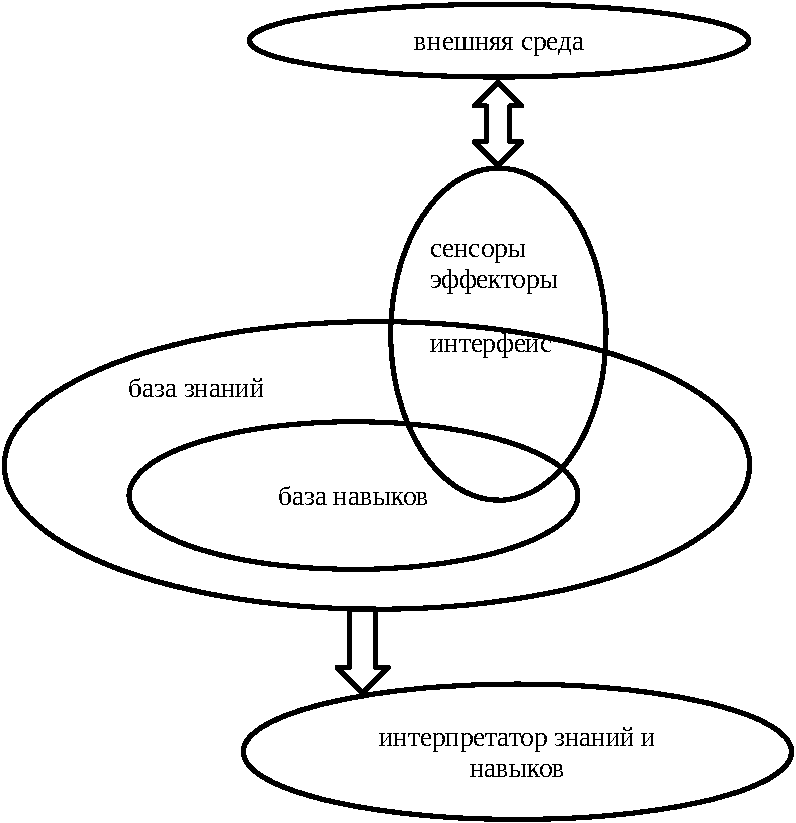
\includegraphics[width=0.5\linewidth]{figures/arch.pdf}\\}

\bigskip
\scnendstruct \scnendcurrentsectioncomment

\end{SCn}

\scsubsection{Предметная область и онтология семантических сетей, семантических языков и семантических моделей баз знаний}
\begin{SCn}

\scnsectionheader{Предметная область и онтология семантических сетей, семантических языков и семантических моделей баз знаний}

\scnstartsubstruct

\scnheader{Предметная область семантических сетей, семантических языков и семантических моделей баз знаний}
\scnsdmainclasssingle{***}
\scnsdclass{смысловое представление информации}
\scnsdrelation{***}

\scnheader{смысловое представление информации}
\scnexplanation{Объективным ориентиром для \textbf{унификации представления информации} в памяти компьютерных систем и ключом к решению многих проблем эволюции компьютерных систем и технологий является \textbf{формализация смысла представляемой информации}.

Уточнение принципов \textbf{смыслового представления информации} основано, во-первых, на четком противопоставление \textbf{внутреннего языка компьютерной системы}, используемого для хранения информации в памяти компьютера, и \textbf{внешних языков компьютерной системы}, используемых для общения (обмена сообщениями) компьютерной системы с пользователями и другими компьютерными системами (смысловое представление используется исключительно для \textbf{внутреннего представления} информации в памяти компьютерной системы), и, во-вторых, на максимально возможном упрощении синтаксиса внутреннего языка компьютерной системы при обеспечении универсальности  путем исключения из такого внутреннего универсального языка средств, обеспечивающих коммуникационную функцию языка (т. е. обмен сообщениями).

Так, например, для внутреннего языка компьютерной системы излишними являются такие коммуникационные средства языка, как союзы, предлоги, разделители, ограничители, склонения, спряжения и другие.

Внешние языки компьютерной системы могут быть как близки ее внутреннему языку, так и весьма далеки от него (как, например, естественные языки).

\textbf{Смысл} – это \textbf{абстрактная} знаковая конструкция, принадлежащая внутреннему языку компьютерной системы, являющаяся \textbf{инвариантом} максимального класса семантически эквивалентных знаковых конструкций (текстов), принадлежащих самым разным языкам, и удовлетворяющая следующим требованиям:
\begin{scnitemize}
    \item \textbf{универсальность} - возможность представления любой информации;
    \item \textbf{отсутствие синонимии знаков} (многократного вхождения знаков с одинаковыми денотатами);
    \item \textbf{отсутствие дублирования информации} в виде семантически эквивалентных текстов (не путать с логической эквивалентностью);
    \item \textbf{отсутствие омонимичных знаков} (в том числе местоимений);
    \item \textbf{отсутствие у знаков внутренней структуры} (атомарный характер знаков);
    \item \textbf{отсутствие склонений, спряжений} (как следствие отсутствия у знаков внутренней структуры);
    \item \textbf{отсутствие фрагментов} знаковой конструкции, \textbf{не являющихся знаками} (разделителей, ограничителей, и т.д.);
    \item \textbf{выделение знаков связей}, компонентами которых могут быть любые знаки, с которыми знаки связей связываются синтаксически задаваемыми отношениями инцидентности.
\end{scnitemize}

Следствием указанных принципов смыслового представления информации в памяти компьютерной системы является то, что знаки сущностей, входящие в смысловое представление информации, \textbf{не являются именами} (терминами) и, следовательно, не привязаны ни к какому естественному языку и не зависят от субъективных терминотворческих пристрастий различных авторов. Это значит, что при коллективной разработке смыслового представления каких-либо информационных ресурсов терминологические споры исключены.

Следствием указанных принципов смыслового представления информации  является также то, что эти принципы приводят к нелинейным знаковым конструкциям (к графовым структурам), что усложняет реализацию памяти компьютерных систем, но существенно упрощает ее логическую организацию (в частности, ассоциативный доступ).

Нелинейность смыслового представления информации обусловлена тем, что: 
\begin{scnitemize}
    \item каждая описываемая сущность, т.е. сущность, имеющая соответствующий ей знак, может иметь неограниченное число связей с другими описываемыми сущностями;
    \item каждая описываемая сущность в смысловом представлении имеет единственный знак, т.к. синонимия знаков здесь запрещена;
    \item все связи между описываемыми сущностями описываются (отражаются, моделируются) связями между знаками этих описываемых сущностей.
\end{scnitemize}

Суть \textbf{универсального смыслового представления информации} можно сформулировать в виде следующих положений:
\begin{scnitemize}
    \item Смысловая знаковая конструкция трактуется как множество знаков, взаимно-однозначно обозначающих различные сущности (денотаты этих знаков) и множество связей между этими знаками;
    \item Каждая связь между знаками трактуется, с одной стороны, как множество знаков, связываемых этой связью, а, с другой стороны, как описание (отражение, модель) соответствующей связи, которая связывает денотаты указанных знаков или денотаты одних знаков непосредственно с другими знаками, или сами эти знаки. Примером первого вида связи между знаками является связь между знаками материальных сущностей, одна из которых является частью другой. Примером второго вида связи между знаками является связь между знаком множества знаков и одним из знаком, принадлежащих этому множеству, а также связь между знаком и знаком файла, являющегося электронным отражением структуры представления указанного знака во внешних знаковых конструкциях. Примерами третьего вида связи между знаками является связь между синонимичными знаками;
    \item Денотатами знаков могут быть (1) не только конкретные (константные, фиксированные), но и произвольные (переменные, нефиксированные) сущности, "пробегающие"\ различные множества знаков (возможных значений), 
    (2) не только реальные (материальные), но и абстрактные сущности (например, числа, точки различных абстрактных пространств), 
    (3) не только "внешние"\,, но и "внутренние"\ сущности, являющиеся множествами знаков, входящих в состав той же самой знаковой конструкции.
\end{scnitemize}

Ключевым свойством языка смыслового представления информации является однозначность представления информации в памяти каждой компьютерной системы, т. е. отсутствие семантически эквивалентных знаковых конструкций, принадлежащих смысловому языку и хранимых в одной смысловой памяти. При этом логическая эквивалентность таких знаковых конструкций допускается и используются, например, для компактного представления некоторых знаний, хранимых в смысловой памяти.

Тем не менее, логической эквивалентностью хранимых в памяти знаковых конструкций увлекаться не следует, т.к. \textbf{логически эквивалентные} знаковые конструкции -- это представление одного и того же знания, но с помощью \textbf{разных наборов понятий}. В отличие от этого \textbf{семантически эквивалентные} знаковые конструкции -- это представление одного и того же знания с помощью одних и тех же понятий. Очевидно, что многообразие возможных вариантов представления одних и тех же знаний в памяти компьютерной системы существенно усложняет решение задач. Поэтому, полностью исключив \textbf{семантическую эквивалентность} в смысловой памяти, необходимо стремиться к минимизации \textbf{логической эквивалентности}. Для этого необходимо грамотное построение системы используемых понятий в виде иерархической системы формальных онтологий ~\cite{Davydenko2018}.

Важным этапом создания универсального формального способа смыслового кодирования знаний был разработанный В.В. Мартыновым Универсальный Семантический Код (УСК)~\cite{Martynov}.

В качестве \textbf{стандарта} универсального смыслового представления информации \textbf{в памяти компьютерных систем} нами предложен \textbf{\textit{SC-код}} (Semantic Computer Code). В отличие от УСК В.В. Мартынова он, во-первых, носит нелинейный характер и, во-вторых, специально ориентирован на кодирование информации в памяти компьютеров нового поколения, ориентированных на разработку семантически совместимых интеллектуальных систем и названных нами \textbf{семантическими ассоциативными компьютерами}. Более подробно это понятие (\textbf{\textit{SC-код}}) рассмотрено в разделе \textit{Предметная область и онтология внутреннего языка ostis-систем -- SC-кода}. Таким образом, основным лейтмотивом предлагаемого нами смыслового представления информации является ориентация на формальную модель памяти нефоннеймановского компьютера, предназначенного для реализации интеллектуальных систем, использующих смысловое представление информации. Особенностями такого представления являются следующие:
\begin{scnitemize}
    \item ассоциативность;
    \item вся информация заключена в конфигурации связей, т.е. переработка информации сводится к реконфигурации связей (к графодинамическим процессам);
    \item прозрачная семантическая интерпретируемость и, как следствие, семантическая совместимость.
\end{scnitemize}

Неявная привязка к фоннеймановским компьютерам присутствует во всех известных моделях представления знаний. Одним из примеров такой зависимости, является, например, обязательность именования описываемых объектов.}

\scnheader{смысловое представление информации}
\scnadvantages{Почему целесообразен переход к \textit{смысловому представлению информации} в памяти \textit{компьютерной системы}: 
\begin{scnitemize}
    \item \textit{смысловое представление информации} есть \uline{объективный}, не зависящий от субъективизма и многообразия синтаксических решений, способ представления информации;
    \item в рамках смыслового представления существенно упрощается процедура интеграции знаний и погружения новых знаний в \textit{базу знаний};
    \item cущественно упрощается процедура приведения различного вида знаний к общему виду (к согласованной системе используемых понятий);
    \item cущественно упрощается процедура интеграции различных \textit{~решателей задач~} и целых \textit{компьютерных систем}; 
    \item существенно упрощается автоматизация перманентного процесса поддержки семантической совместимости (согласованности понятий и онтологий) для \textit{компьютерных систем} в условиях их постоянного совершенствования;
    \item в рамках смыслового представления информации достаточно легко осуществляется переход от информационных конструкций к информационным метаконструкциям путем введения узлов семантической сети, обозначающих информационные конструкции, а также дуг, связывающих эти узлы со всеми элементами обозначаемой им информационной конструкции;
    \item на основе \textit{стандарта смыслового представления информации} существенно упрощается интеграция различных дисциплин в области искусственного интеллекта, т.е. построение общей формальной теории интеллектуальных компьютерных систем, так как для построения общей формальной модели интеллектуальных компьютерных систем необходим базовый язык, в рамках которого можно было бы легко переходить от информации (от знаний) к \textbf{метаинформации} (к метазнаниям, к спецификациям исходных знаний).  Это подтверждается тем, что:
    \begin{scnitemizeii}
        \item подавляющее число понятий искусственного интеллекта носит метаязыковой характер;
        \item формальное смысловое уточнение почти каждого понятия искусственного интеллекта требует предшествующего формального уточнения соответствующего языка-объекта. Так, например, как можно строго говорить о языке онтологий (т.е. языке спецификации предметных областей), не уточнив язык представления самих этих предметных областей. Как можно строго говорить о языке описания способов обработки информации, не уточнив язык представления самой этой обрабатываемой информации.
    \end{scnitemizeii}
\end{scnitemize}}

\scnendstruct

\end{SCn}

\scsubsection{Предметная область и онтология агентно-ориентированных семантических моделей решателей задач}
\begin{SCn}

\scnsectionheader{\currentname}

\scnstartsubstruct

\scnheader{Предметная область многоагентных моделей решения задач, основанных на смысловом представлении информации}
\scniselement{предметная область}
\scnsdmainclasssingle{многоагентный подход к обработке информации}
\scnsdclass{интеграция решателей задач}
\scnsdrelation{совместимость моделей решения задач*}

\scnheader{агентно-ориентированный подход к обработке информации}
\scnnote{В качестве основы унификации принципов обработки информации в компьютерных системах предлагается использовать \textit{агентно-ориентированный подход к обработке информации}, обладающий рядом важных достоинств.}
\scnrelfromset{достоинства}{\scnfileitem{Автономность (независимость) агентов, что позволяет локализовать изменения, вносимые в систему при ее эволюции, и снизить соответствующие трудозатраты.};
\scnfileitem{Децентрализация обработки, т.е. отсутствие единого контролирующего центра, что также позволяет локализовать вносимые в систему изменения.};
\scnfileitem{Возможность параллельной работы разных информационных процессов, соответствующих как одному агенту, так и разным агентам, как следствие, -- возможность распределенного решения задач. Однако возможность параллельного выполнения информационных процессов подразумевает наличие средств синхронизации такого выполнения, разработка которых является отдельной задачей.};
\scnfileitem{Активность агентов и многоагентной системы в целом, дающая возможность при общении с такой системой не указывать явно способ решения поставленной задачи, а формулировать задачу в \uline{декларативном ключе}.}}
\scnaddlevel{1}
	\scnrelfrom{источник}{\scncite{Wooldridge2009}}
\scnaddlevel{-1}
\scnrelfromset{недостатки современного состояния}{\scnfileitem{Знания агента представляются при помощи узкоспециализированных языков, зачастую не предназначенных для представления знаний в широком смысле и онтологий в частности.};
\scnfileitem{Большинство современных многоагентных систем предполагает, что взаимодействие агентов осуществляется путем обмена сообщениями непосредственно от агента к агенту.};
\scnfileitem{Логический уровень взаимодействия агентов жестко привязан к физическому уровню реализации многоагентной системы.};
\scnfileitem{Среда, с которой взаимодействуют агенты, уточняется отдельно разработчиком для каждой многоагентной системы, что приводит к существенным накладным расходам и несовместимости таких многоагентных систем.}}
\scnaddlevel{1}
\scnrelfromset{принципы устранения}{
\scnfileitem{Коммуникацию агентов предлагается осуществлять путем спецификации (в общей памяти компьютерной системы) действий (процессов), выполняемых агентами и направленных на решение задач.}
\scnaddlevel{1}
	\scntext{детализация}{Коммуникацию агентов предлагается осуществлять по принципу ``доски объявлений'', однако в отличие от классического подхода в роли сообщений выступают спецификации в общей семантической памяти выполняемых агентами действий (процессов), направленных на решение каких-либо задач, а в роли среды коммуникации выступает сама эта семантическая память. Такой подход позволяет: 
	\begin{scnitemize}
		\item исключить необходимость разработки специализированного языка для обмена сообщениями;
		\item обеспечить "обезличенность"{} общения, т. е. каждый из агентов в общем случае не знает, какие еще агенты есть в системе, кем сформулирован и кому адресован тот или иной запрос. Таким образом, добавление или удаление агентов в систему не приводит к изменениям в других агентах, что обеспечивает модифицируемость всей системы;
		\item агентам, в том числе конечному пользователю, формулировать задачи в \uline{декларативном ключе}, т. е. не указывать для каждой задачи способ ее решения. Таким образом, агенту заранее не нужно знать, каким образом система решит ту или иную задачу, достаточно лишь специфицировать конечный результат;
		\item сделать средства коммуникации агентов и синхронизации их деятельности более понятными разработчику и пользователю системы, не требующими изучения специальных низкоуровневых типов данных и форматов сообщений. Таким образом повышается доступность предлагаемых решений широкому кругу разработчиков.
	\end{scnitemize}
	Следует отметить, что такой подход позволяет при необходимости организовать обмен сообщениями между агентами напрямую и, таким образом, может являться основой для моделирования многоагентных систем, предполагающих другие способы взаимодействия между агентами.}
\scnaddlevel{-1}
;
\scnfileitem{В роли внешней среды для агентов выступает та же общая память, в которой формулируются задачи и посредством которой осуществляется взаимодействие агентов. Такой подход обеспечивает унификацию среды для различных систем агентов, что, в свою очередь, обеспечивает их совместимость.};
\scnfileitem{Спецификация каждого агента описывается средствами языка представления знаний в той же памяти, что позволяет:
	\begin{scnitemize}
		\item минимизировать число специализированных средств, необходимых для спецификации агентов, как языковых, так и инструментальных;
		\item с одной стороны -- минимизировать необходимую в общем случае спецификацию агента, которая включает условие его инициирования и программу, описывающую алгоритм работы агента, с другой стороны -- обеспечить возможность произвольного расширения спецификации для каждого конкретного случая, в том числе возможность реализации различных современных моделей спецификации агента.
	\end{scnitemize}};
\scnfileitem{Синхронизацию деятельности агентов предполагается осуществлять на уровне выполняемых ими процессов, направленных на решение тех или иных задач в общей семантической памяти. Таким образом, каждый агент трактуется как некий абстрактный процессор, способный решать задачи определенного класса. При таком подходе необходимо решить задачу обеспечения взаимодействия параллельных асинхронных процессов в общей семантической памяти, для решения которой можно заимствовать и адаптировать решения, применяемые в традиционной линейной памяти. При этом вводится дополнительный класс агентов -- метаагенты, задачей которых является решение возникающих проблемных ситуаций, таких как взаимоблокировки};
\scnfileitem{Каждый информационный процесс в любой момент времени имеет ассоциативный доступ к необходимым фрагментам базы знаний, хранящейся в семантической памяти, за исключением фрагментов, заблокированных другими процессами в соответствии с соответствующим механизмом синхронизации. Таким образом, с одной стороны, исключается необходимость хранения каждым агентом информации о внешней среде, с другой стороны, каждый агент, как и в классических многоагентных системах, обладает только частью всей информации, необходимой для решения задачи.\\
Важно отметить, что в общем случае невозможно априори предсказать, какие именно знания, модели и способы решения задач понадобятся системе для решения конкретной задачи. В связи с этим необходимо обеспечить, с одной стороны, возможность доступа ко всем необходимым фрагментам базы знаний (в пределе -- ко всей базе знаний), с другой стороны -- иметь возможность локализовать область поиска пути решения задачи, например, рамками одной \textit{предметной области}.\\
Каждый из агентов обладает набором ключевых элементов (как правило, понятий), которые он использует в качестве отправных точек при ассоциативном поиске в рамках базы знаний. Набор таких элементов для каждого агента уточняется на этапах проектирования многоагентной системы в соответствии с рассматриваемой ниже методикой. Уменьшение числа ключевых элементов агента делает его более универсальным, однако снижает эффективность его работы за счет необходимости выполнения дополнительных  операций.}}
\scnaddlevel{1}
\scnnote{Предлагаемый подход позволяет рассматривать решатель задач как иерархическую систему. Некий целостный коллектив агентов, реализующий какую-либо подсистему решателя (например, машину дедуктивного вывода, подсистему верификации базы знаний и т. д.), может рассматриваться как единый неатомарный агент, поскольку коллективы агентов и отдельные агенты работают в соответствии с одними и теми же принципами.}
\scnaddlevel{-2}

\scnheader{совместимость моделей решения задач*}
\scnnote{\textbf{\textit{совместимость моделей решения задач*}} -- это возможность одновременного использования разными моделями решения задач одних и тех же информационных ресурсов.}
\scnrelfromset{принципы реализации}{
\scnfileitem{Вся информация, хранимая в памяти каждой ostis-системы и используемая \textit{\textbf{решателем задач}} (как собственно обрабатываемая информация, так и хранимые в памяти интерпретируемые методы, например, различного вида программы), записывается в форме смыслового представления этой информации}; 
\scnfileitem{Собственно решение каждой задачи осуществляется коллективом агентов, работающих над общей для них смысловой (семантической) памятью и выполняющих интерпретацию хранимых в этой же памяти \textit{методов}.}}

\scnheader{интеграция решателей задач}
\scnsubset{процесс}
\scnrelfromvector{алгоритм реализации}{
\scnfileitem{Объединение множества методов первого решателя и множества методов второго решателя};	
\scnfileitem{Интеграция множества методов первого решателя и множества методов второго решателя путем взаимного погружения соответствующих информационных конструкций друг в друга, т.е. путем склеивания синонимов, а также путем выравнивания используемых ими понятий.};
\scnfileitem{Объединение множества агентов, входящих в состав первого решателя, со множеством агентов, входящих во второй решатель задач.}}
\scnexplanation{Таким образом, унификация моделей решения задач путем приведения этих моделей к виду семантических моделей (т. е. моделей обработки информации, представленной в смысловой форме) повышает уровень совместимости этих моделей благодаря наличию прозрачной процедуры интеграции информации, представленной в смысловой форме, и тривиальной процедуры объединения множеств \textit{агентов}. Простота процедуры объединения множеств \textit{агентов}, соответствующих разным решателя задач, обусловлена тем, что непосредственного взаимодействия между этими агентами нет, а инициирование каждого из них определяется им самим, а также \uline{текущим состоянием} хранимой в памяти информации.}

\bigskip

\scnendstruct \scnendcurrentsectioncomment

\end{SCn}

\scsubsection{Предметная область и онтология семантических моделей интерфейсов компьютерных систем}

\scsectionfinish{sem_mod_comp_sys}

\input{Contents/chapter1/sem_sys_arch.tex}

\begin{SCn}

\scnheader{язык смыслового представления информации}
\scnidtf{смысловой язык}
\scnidtf{семантический язык}
\scnsubdividing{язык смыслового представления информации, не являющийся языком семантических сетей;
язык семантических сетей}

\scnheader{язык семантических сетей}
\scnexplanation{Несмотря на то, что синтаксическая структура семантической сети во многом носит \uline{объективный} характер, поскольку определяется конфигурацией описываемых связей между описываемыми сущностями. Тем не менее, можно говорить о разных \textit{языках семантических сетей}, каждому из которых соответствует свой \textit{алфавит*} элементов (синтаксически атомарных фрагментов) \textit{семантических сетей}. При атом языки семантических сетей могут быть как специализированными, так и универсальными. Задача каждого из этих \textit{языков} -- обеспечить в рамках \textit{языка} полное отсутствие многообразия синтаксических форм представления одной и той же информации.}

\scnsubset{язык}
\scnaddlevel{1}
\scnidtf{множество информационных конструкций, для которого существуют, причем не обязательно в формализованном виде, (1) правила построения синтаксически корректных информационных конструкций, а также (2) правила, позволяющие установить семантическую корректность правильно построенных (синтаксически корректных) информационных конструкций}
\scnaddlevel{-1}
\scnidtf{язык, информационными конструкциями которого являются семантические сети и в рамках которого обеспечивается полное отсутствие многообразия форм представления одной и той же информации}
\scnidtf{графовый (нелинейный) язык смыслового представления информации}

\scnsubdividing{специализированный язык семантических сетей
\scnaddlevel{1}
\scnidtf{язык семантических сетей, семантическая мощность которого ограничена соответствующей предметной областью}
\scnaddlevel{-1};
универсальный язык емантических сетей
\newline
\scnaddlevel{1}
\scnnote{Человечество давно и широко использует различные специализированные языки семантических сетей -- язык принципиальных электрических схем, язык блок-схем программ, язык генеалогических деревьев и др. Но в настоящее время актуальным является создание такого \textit{универсального языка семантических сетей}
\begin{scnitemize}
	\item синтаксис и семантика которого были бы максимально просты;
	\item по отношению к которому все используемые специализированные языки были бы его подъязыками*;
	\item который был бы приспособлен к использованию в качестве внутреннего языка интеллектуальных компьютерных систем и компьютеров следующего поколения;
	\item который был бы удобной основой как для обмена информацией между интеллектуальными компьютерными системами, так и для общения интеллектуальных клмпьютерных систем с их пользователями
\end{scnitemize}
\scnaddlevel{-1}
}}
\scnsubdividing{язык нерафинированных семантических сетей;
язык рафинированных семантических сетей}

\scnheader{следует отличать*}
\scnhaselementset{язык семантических сетей
\scnaddlevel{1}
\scnidtf{язык семантических сетей, рассматриваемых как \uline{абстрактные} графовые структуры, в которых не уточняется способ их кодирования}
\scnhaselement{SC-код}
\scnaddlevel{-1};
графодинамический язык семантических сетей
\scnaddlevel{1}
\scnidtf{язык графического изображения (визуализации) семантических сетей}
\scnidtf{язык, текстами которого являются рисунки семантичеких сетей}
\scnhaselement{SCg-код}
\scnaddlevel{-1}}

\scnheader{универсальный язык семантических сетей}
\scnnote{Если ставить задачу разработки \uline{универсального}(!) языка, текстами которого являются графовые структуры, то классических графовых структур явно недостаточно. Так, например:
\begin{scnitemize}
	\item по аналогии с переходом от ребер к ребрам и гиперребрам необходим переход от дуг к ориентированным связкам, связывающим более чем два компонента и в рамках которых эти компоненты могут иметь разные роли, которые необходимо явно указывать (классическим видом таких связок являются кортежи);
	\item в семантических сетях, представляющих некоторые виды знаний, некоторые связки (ребра, дуги, гиперребра, ориентированные связки, связывающие более двух компонентов) могут быть компонентами других связок;
	\item в семантических сетях, представляющих различного вида метазнания необходимо вводить узлы, обозначающие целые фрагменты (подграфы) этих же семантических сетей, и, соответственно, вводить дуги, связывающие каждый из этих узлов со всеми элементами подграфа, обозначаемого этим узлом.
\end{scnitemize}}

\end{SCn}
%
\scchapter{Предметная область и онтология знаний и баз знаний ostis-систем}
\label{sec:sd_knowledge}
\begin{SCn}

\scnsectionheader{\currentname}

\scnstartsubstruct

\scnrelfromlist{дочерний раздел}{Предметная область и онтология множеств
    \scnaddlevel{1}
    \scnidtf{Предметная область и онтология \textit{знаний о множествах}}
        \scnaddlevel{1}
        \scnnote{\textit{знания о множествах} являются \uline{частным видом} \textit{знаний} и, следовательно, общие свойства сущностей, описываемых знаниями, могут наследоваться \textit{Предметной областью и онтологией множеств}}
        \scnaddlevel{-1}
    \scnaddlevel{-1}
;Предметная область и онтология связок и отношений
;Предметная область и онтология параметров, величин и шкал
;Предметная область и онтология чисел и числовых структур
;Предметная область и онтология структур
;Предметная область и онтология темпоральных сущностей
;Предметная область и онтология темпоральных сущностей баз знаний ostis-систем
;Предметная область и онтология семантических окрестностей
;Предметная область и онтология предметных областей
;Предметная область и онтология онтологий
;Предметная область и онтология логических формул, высказываний и формальных теорий
;Предметная область и онтология внешних информационных конструкций и файлов ostis-систем
;Глобальная предметная область действий и задач и соответствующая ей онтология методов и технологий}

\scnheader{Предметная область знаний и баз знаний ostis-систем}
\scniselement{предметная область}
\scnsdmainclasssingle{знание}
\scnhaselementlist{исследуемый класс классов}{вид знаний;отношение, заданное на множестве знаний}

\scnheader{знание}
\scnidtf{синтаксически корректная (для соответствующего языка) и семантически целостная информационная конструкция}
\scnsubset{информационная конструкция}
    \scnaddlevel{1}
    \scniselementrole{класс объектов исследования}{\nameref{intro_lang}}
    \scnaddlevel{-1}
\scnaddlevel{1}
\scnrelboth{следует отличать}{данные}
\scnaddlevel{1}
\scnexplanation{
	Принципиальные различия знаний и данных:
	
	\begin{scnitemize}
		\item \textit{Интерпретация}. Хранимые данные могут быть интерпретированы только человеком или программой. Данные не несут информации. Знания содержат как данные, так и их описание (правила интерпретации)
		\item \textit{Наличие связей классификации}. Данные не имеют эффективного описания связей между различными типами данных. Знания структурированы, так как можно установить соответствие между единицами знаний.
		\item \textit{Наличие ситуационных связей}. Связи описывают множество текущих ситуаций объекта. Данные трудно поддаются анализу. Из структуры и состава знаний по ситуации возможно построение процедур анализа знаний.
	\end{scnitemize}
}
\scnaddlevel{1}
\scnrelfrom{цитата}{\scncite{Helpiks2015}}
\scnaddlevel{-1}
\scnaddlevel{-1}
\scnaddlevel{-1}
\scnrelfrom{покрытие}{вид знаний
    \scnidtf{Множество \uline{всевозможных} видов знаний}
    \scnnote{Тот факт, что семейство \textit{видов знаний} является \textit{покрытием} Множества всевозможных \textit{знаний}, означает то, что каждое \textit{знание} принадлежит по крайней мере одному выделенному нами \textit{виду знаний}}}

    
    
   \scnheader{вид знаний}
\scnhaselement{спецификация}
    \scnaddlevel{1}
    \scnidtf{описание заданной сущности}
    \scnsuperset{спецификация материальной сущности}
    \scnsuperset{спецификация обратной сущности, не являющейся множеством}
        \scnaddlevel{1}
        \scnsuperset{спецификация геометрической точки}
        \scnsuperset{спецификация числа}
        \scnaddlevel{-1}
    \scnsuperset{спецификация множества}
        \scnaddlevel{1}
        \scnsuperset{спецификация связи}
        \scnsuperset{спецификация структуры}
        \scnsuperset{спецификация класса}
            \scnaddlevel{1}
            \scnsuperset{спецификация класса сущностей, не являющихся множествами}
            \scnsuperset{спецификация отношения}
                \scnaddlevel{1}
                \scnidtf{спецификация класса связей (связок)}
                \scnaddlevel{-1}
            \scnsuperset{спецификация класса классов}
                \scnaddlevel{1}
                \scnsuperset{спецификация параметра}
                \scnaddlevel{-1}
            \scnsuperset{спецификация класса структур}
            \scnsuperset{спецификация понятий}
                \scnaddlevel{1}
                \scnsuperset{пояснение}
                \scnsuperset{определение}
                \scnsuperset{утверждение}
                    \scnaddlevel{1}
                    \scnidtf{утверждение, описывающее свойства экземпляров (элементов) специфицируемого понятия}
                    \scnidtf{закономерность}
                    \scnaddlevel{-1}
                \scnaddlevel{-1}
            \scnaddlevel{-1}
        \scnaddlevel{-1}
    \scnsuperset{семантическая окрестность}
    \scnsuperset{однозначная спецификация}
    \scnsuperset{сравнительный анализ}
    \scnsuperset{достоинства}
    \scnsuperset{недостатки}
    \scnsuperset{структура специфицируемой сущности}
    \scnsuperset{принципы, лежащие в основе}
    \scnsuperset{обоснование предлагаемого решения}
        \scnaddlevel{1}
        \scnidtf{аргументация предлагаемого решения}
        \scnaddlevel{-1}
    \scnaddlevel{-1}

\scnhaselement{сравнение}

\scnhaselement{высказывание}
    \scnaddlevel{1}
    \scnsuperset{фактографическое высказывание}
    \scnsuperset{закономерность}
    \scnaddlevel{-1}

\scnhaselement{формальная теория}

\scnhaselement{предметная область}

\scnhaselement{предметная область и онтология
    \scnaddlevel{1}
    \scnidtf{предметная область и её онтология}
    \scnidtf{предметная область и соответствующая ей объединенная онтология}
    \scnaddlevel{-1}} 
 
\scnhaselement{метазнание}
    \scnaddlevel{1}
    \scnidtf{спецификация знания}
    \scnsuperset{аннотация}
    \scnsuperset{введение}
    \scnsuperset{предисловие}
    \scnsuperset{заключение}
    \scnsuperset{онтология}
        \scnaddlevel{1}
        \scnsuperset{онтология предметной области}
            \scnaddlevel{1}
            \scnsuperset{структурная онтология предметной области}
            \scnsuperset{теоретико-множественная онтология предметной области}
            \scnsuperset{логическая онтология предметной области}
            \scnsuperset{терминологическая онтология предметной области}
            \scnsuperset{объединенная онтология предметной области}
            \scnaddlevel{-1}
        \scnaddlevel{-1}
    \scnaddlevel{-1}

\scnhaselement{задача}
    \scnaddlevel{1}
    \scnidtf{спецификация действия}
    \scnaddlevel{-1}
\scnhaselement{план}

\scnhaselement{протокол}

\scnhaselement{результативная часть протокола}

\scnhaselement{метод}

\scnhaselement{технология}

\scnhaselement{история использования предметной области и её онтологии по решению информационных задач}
\scnhaselement{история использования предметной области и её онтологии по решению задач во внешней среде}
\scnhaselement{история эволюции предметной области и её онтологии}

\scnhaselement{база знаний}
    \scnaddlevel{1}
    \scnidtf{совокупность знаний, хранимых в памяти интеллектуальной компьютерной системы и \uline{достаточных} для того, чтобы указанная система удовлетворяла соответствующим предъявляемым к ней требованиям (в частности, чтобы она имела соответствующий уровень интеллекта)}
    \scnidtf{систематизированная совокупность знаний, хранимая в памяти интеллектуальной компьютерной системы и достаточная для обеспечения целенаправленного (целесообразного, адекватного) функционирования (поведения) этой системы как в своей внешней среде, так и в своей внутренней среде (в собственной базе знаний)}
    \scnrelfromset{обобщенная декомпозиция}{согласованная часть базы знаний
        \scnaddlevel{1}
        \scnidtf{часть базы знаний, признанная коллективом авторов на текущий момент}
        \scnaddlevel{-1}
    ;история эксплуатации базы знаний;история эволюции базы знаний;план эволюции базы знаний
        \scnaddlevel{1}
        \scnidtf{система специфицированных и согласованных действий авторов базы знаний, направленных на повышение её качества}
        \scnaddlevel{-1}}
    \scnnote{Основным факторами, определяющими качество интеллектуальной компьютерной системы, являются:
    \begin{scnitemize}
        \item качественная структуризация (систематизация) и \uline{стратификация} базы знаний интеллектуальной компьютерной системы, а также
        \item систематизация и стратификация \uline{деятельности}, которая осуществляется интеллектуальной компьютерной системой и спецификация которой является важнейшей частью базы знаний этой системы (Смотрите Раздел \textit{Глобальная предметная область действий и задач и соответствующая ей онтология методов и технологий}).
    \end{scnitemize}}
    \scnaddlevel{-1}
\scnnote{Даже небольшой перечень \textit{видов знаний} свидетельствует об огромном многообразии \textit{видов знаний}}

\scnheader{знание}
\scnsubdividing{декларативное знание
    \scnaddlevel{1}
    \scnidtf{\textit{знание}, имеющее \uline{только} \textit{денотационную семантику}, которая представляется в виде семантической \textit{спецификации} системы \textit{понятий}, используемых в этом \textit{знании}}
    \scnaddlevel{-1}
;процедурное знание
    \scnaddlevel{1}
    \scnidtf{\textit{знание}, имеющее не только \textit{денотационную семантику}, но и \textit{операционную семантику}, которая представляется в виде семейства \textit{спецификаций агентов}, осуществляющих интерпретацию \textit{процедурного знания}, направленную на решение некоторой инициированной \textit{задачи}}
    \scnidtf{функционально интерпретируемое знание, обеспечивающее решение либо конкретной задачи, либо некоторого множества инициируемых задач}
    \scnsuperset{задача}
        \scnaddlevel{1}
        \scnidtf{формулировка конкретной задачи}
        \scnsuperset{декларативная формулировка задачи}
        \scnsuperset{процедурная формулировка задачи}
        \scnaddlevel{-1}
    \scnsuperset{план}
        \scnaddlevel{1}
        \scnidtf{план решения конкретной задачи}
        \scnidtf{контекст конкретной задачи, предоставляющий всю информацию для решения всех подзадач для указанной конкретной задачи}
        \scnidtf{описание системы подзадач некоторой задачи}
        \scnaddlevel{-1}
    \scnsuperset{метод}
        \scnaddlevel{1}
        \scnidtf{обобщенное описание плана решения любой задачи из некоторого заданного класса задач}
        \scnaddlevel{-1}
    \scnsuperset{навык}
        \scnaddlevel{1}
        \scnidtf{метод, детализированный до уровня элементарных подзадач}
        \scnaddlevel{-1}
    \scnaddlevel{-1}}
    
\scnheader{отношение, заданное на множестве знаний}
\scnhaselement{дочернее знание*}
    \scnaddlevel{1}
    \scnidtf{знание, которое от "материнского"{} знания наследует все описанные там свойства объектов исследования}
    \scnnote{Факт наследования свойств описываемых объектов от "материнского"{} знания подчеркивается использованием прилагательного "дочернее"{} в sc-идентификаторе данного отношения, заданного на множестве знаний}
    \scnsuperset{дочерний раздел*}
        \scnaddlevel{1}
        \scnidtf{частный раздел*}
        \scnaddlevel{-1}
    \scnsuperset{дочерняя предметная область и онтология*}
    \scnaddlevel{-1}
\scnhaselement{спецификация*}
    \scnaddlevel{1}
    \scnidtf{быть знанием, которое является спецификацией (описанием) заданной сущности}
    \scnnote{специфицируемой сущностью может быть сущность любого вида, в том числе, и другое знание}
    \scnaddlevel{-1}
\scnhaselement{онтология*}
    \scnaddlevel{1}
    \scnidtf{быть семантической спецификацией заданного знания*}
    \scnaddlevel{-1}
\scnhaselement{семантическая эквивалентность*}
\scnhaselement{следовательно*}
    \scnaddlevel{1}
    \scnidtf{логическое следствие*}
    \scnaddlevel{-1}
\scnhaselement{логическая эквивалентность*}   
    
\bigskip    
\scnendstruct \scnendcurrentsectioncomment

\end{SCn}

\scsection{Предметная область и онтология множеств}
\label{sec:sd_sets}
\begin{SCn}

\scnsectionheader{\currentname}

\scnstartsubstruct

\scnheader{Предметная область множеств}
\scnidtf{Теоретико-множественная предметная область}
\scnidtf{Предметная область теории множеств}
\scnidtf{Предметная область, объектами исследования которой являются множества}
\scniselement{предметная область}
\scnsdmainclasssingle{множество}
\scnsdclass{конечное множество;бесконечное множество;счетное множество;несчетное множество;множество без кратных элементов;мультимножество;кратность принадлежности;класс;класс первичных sc-элементов;класс множеств;класс структур;класс классов;нечеткое множество;четкое множество;множество первичных сущностей;семейство множеств;нерефлексивное множество;рефлексивное множество;множество первичных сущностей и множеств;сформированное множество;несформированное множество;пустое множество;синглетон;пара;пара разных элементов;пара-мультимножество;тройка;кортеж;декартово произведение;булеан;мощность множества}
\scnsdrelation{принадлежность*;пример\scnrolesign;включение*;строгое включение*;объединение*;разбиение*;пересечение*;пара пересекающихся множеств*;попарно пересекающиеся множества*;пересекающиеся множества*;пара непересекающихся множеств*;попарно непересекающиеся множества*;непересекающиеся множества*;разность множеств*;симметрическая разность множеств*;декартово произведение*;семейство подмножеств*;булеан*;равенство множеств*}

\scnheader{множество}
\scnidtf{множество sc-элементов}
\scnidtf{sc-множество}
\scnidtf{множество знаков}
\scnidtf{множество знаков описываемых сущностей}
\scnidtf{семантически нормализованное множество}
\scnidtf{sc-знак множества sc-элементов}
\scnidtf{sc-знак множества sc-знаков}
\scnidtf{sc-текст}
\scnidtf{текст SC-кода}
\scnidtf{SC-код}
\scnsubdividing{конечное множество;бесконечное множество}
\scnsubdividing{множество без кратных элементов;мультимножество}
\scnsubdividing{связка;класс\\
    \scnaddlevel{1}
    \scnidtf{sc-элемент, обозначающий класс sc-элементов}
    \scnidtf{sc-знак множества sc-элементов, эквивалентных в том или ином смысле}
    \scnaddlevel{-1}
    ;структура\\
    \scnaddlevel{1}
    \scnidtf{sc-знак множества sc-элементов, в состав которого входят sc-связки или структуры, связывающие эти sc-элементы}
    \scnaddlevel{-1}}
\scnsubdividing{четкое множество;нечеткое множество}
\scnsubdividing{множество первичных сущностей;множество множеств;множество первичных сущностей и множеств}
\scnsubdividing{рефлексивное множество;нерефлексивное множество}
\scnsubdividing{сформированное множество;несформированное множество}
\scnsubdividing{кортеж;неориентированное множество}
\scnsuperset{пустое множество}
\scnsuperset{синглетон}
\scnsuperset{пара}
\scnsuperset{тройка}
\scnexplanation{Под \textbf{\textit{множеством}} понимается соединение в некое целое M определённых хорошо различимых предметов m нашего созерцания или нашего мышления (которые будут называться «элементами» множества M). 

\textbf{\textit{множество}} – мысленная сущность, которая связывает одну или несколько сущностей в целое.

Более формально \textbf{\textit{множество}} – это абстрактный математический объект, состоящий из элементов. Связь множеств с их элементами задается бинарным ориентированным отношением \textbf{\textit{принадлежность*}}.

\textbf{\textit{множество}} может быть полностью задано следующими тремя способами:
\begin{scnitemize}
    \item путем перечисления (явного указания) всех его элементов (очевидно, что таким способом можно задать только конечное множество)
    \item с помощью определяющего высказывания, содержащего описание общего характеристического свойства, которым обладают все те и только те объекты, которые являются элементами (т.е. принадлежат) задаваемого множества.
    \item с помощью теоретико-множественных операций, позволяющих однозначно задавать новые множества на основе уже заданных (это операции объединения, пересечения, разности множеств и др.)
\end{scnitemize}
Для любого семантически ненормализованного \textbf{\textit{множества}} существует единственное семантически нормализованное \textbf{\textit{множество}}, в котором все элементы, не являющиеся знаками множеств, заменены на знаки множеств.}

\scnheader{принадлежность*}
\scnidtf{принадлежность элемента множеству*}
\scnidtf{отношение принадлежности элемента множеству*}
\scniselement{бинарное отношение}
\scniselement{ориентированное отношение}
\scnexplanation{\textbf{\textit{принадлежность*}} – это бинарное ориентированное отношение, каждая связка которого связывает множество с одним из его элементов. Элементами отношения \textbf{\textit{принадлежность*}} по умолчанию являются \textit{позитивные sc-дуги принадлежности}.}

\scnheader{конечное множество}
\scnidtf{множество с конечным числом элементов}
\scnexplanation{\textbf{\textit{конечное множество}} – это \textit{множество}, количество элементов которого конечно, т.е. существует неотрицательное целое число \textit{k}, равное количеству элементов этого множества.}

\scnheader{бесконечное множество}
\scnidtf{множество с бесконечным числом элементов}
\scnsubdividing{счетное множество;несчетное множество}
\scnexplanation{\textbf{\textit{бесконечное множество}} – это \textit{множество}, в котором для любого натурального числа \textit{n} найдётся конечное подмножество из \textit{n} элементов.}

\scnheader{счетное множество}
\scnexplanation{\textbf{\textit{счетное множество}} – это \textit{бесконечное множество}, для которого существует \textit{взаимно-однозначное соответствие} с натуральным рядом чисел.}

\scnheader{несчетное множество}
\scnidtf{континуальное множество}
\scnexplanation{\textbf{\textit{несчетное множество}} - это \textit{бесконечное множество}, элементы которого невозможно пронумеровать натуральными числами.}

\scnheader{множество без кратных элементов}
\scnidtf{классическое множество}
\scnidtf{канторовское множество}
\scnidtf{множество, состоящее из разных элементов}
\scnidtf{множество без кратного вхождения элементов}
\scnidtf{множество, все элементы которого входят в него однократно}
\scnidtf{множество, не имеющее кратного вхождения элементов}
\scnexplanation{\textbf{\textit{множество без кратных элементов}} - это \textit{множество}, для каждого элемента которого существует только одна пара принадлежности, выходящая из знака этого множества в указанный элемент.}

\scnheader{мультимножество}
\scnidtf{множество, имеющее кратные вхождения хотя бы одного элемента}
\scnidtf{множество, по крайней мере один элемент которого входит в его состав многократно}
\scnexplanation{\textbf{\textit{мультимножество}} - это \textit{множество}, для которого существует хотя бы одна кратная пара принадлежности, выходящая из знака этого множества.}

\scnheader{кратность принадлежности}
\scnidtf{кратность принадлежности элемента}
\scnidtf{кратность вхождения элемента во множество}
\scniselement{параметр}
\scnexplanation{\textbf{\textit{кратность принадлежности}} - \textit{параметр}, значением которого являются числовые величины, показывающие сколько раз входит тот или иной элемент в рассматриваемое множество. Элементами данного параметра являются классы \textit{позитивных sc-дуг принадлежности}, связывающих данное множество с элементом, кратность вхождения которого в данное множество мы хотим задать.

Таким образом, кратное вхождение элемента в мультимножество может быть задано как явным указанием \textit{позитивных sc-дуг принадлежности} этого элемента данному \textit{множеству}, так и «склеиванием» этих дуг в одну и включением ее в некоторый класс \textbf{\textit{кратности принадлежности}}.}
\scnrelfrom{описание примера}{
\scnfilescg{figures/sd_sets/multiplicityOfMembership.png}
}

\scnheader{класс}
\scnidtf{класс sc-элементов}
\scnsubdividing{класс первичных sc-элементов;класс множеств}
\scnexplanation{\textbf{\textit{класс}} – множество элементов, обладающих какими-либо явно указываемыми общими свойствами.}

\scnheader{класс первичных sc-элементов}
\scnexplanation{\textbf{\textit{класс первичных sc-элементов}} – класс, элементами которого являются только \textit{sc-элементы}, не являющиеся знаками множеств.}

\scnheader{класс множеств}
\scnsubdividing{отношение;класс структур;класс классов}
\scnexplanation{\textbf{\textit{класс множеств}} – класс, элементами которого являются только \textit{sc-элементы}, являющиеся знаками множеств.}

\scnheader{класс структур}
\scnexplanation{\textbf{\textit{класс структур}} – класс, элементами которого являются \textit{структуры}.}

\scnheader{класс классов}
\scnexplanation{\textbf{\textit{класс классов}} – класс, элементами которого являются \textit{классы}.}

\scnheader{нечеткое множество}
\scnexplanation{\textbf{\textit{нечеткое множество}} – это \textit{множество}, которое представляет собой совокупность элементов произвольной природы, относительно которых нельзя точно утверждать – обладают ли эти элементы некоторым характеристическим свойством, которое используется для задания этого нечеткого множества. Принадлежность элементов такому множеству указывается при помощи \textit{нечетких позитивных sc-дуг принадлежности}.}

\scnexplanation{Важной особенностью нечетких множеств является предоставление основы для нежесткого взаимодействия классов, кодируемых символьными метками и числовыми значениями. Это возможно благодаря тому, что нечеткие множества могут моделировать восприятие. Использование нечетких классов в задачах классификации избавляет от необходимости произвольно типизировать пограничные случаи в начале этапа рассуждений.}
\scnaddlevel{1}
\scnrelto{цитата}{\scncite{Dubois20031}}
\scnaddlevel{-1}

\scnheader{четкое множество}
\scnexplanation{\textbf{\textit{четкое множество}} – это \textit{множество}, принадлежность элементов которому достоверна и указывается при помощи \textit{четких позитивных sc-дуг принадлежности}.}

\scnheader{множество первичных сущностей}
\scnsuperset{класс первичных сущностей}
\scnsubset{множество}
\scnexplanation{\textbf{\textit{множество первичных сущностей}} – это \textit{множество}, элементы которого не являются знаками множеств.}

\scnheader{семейство множеств}
\scnidtf{множество множеств}
\scnsuperset{класс классов}
\scnexplanation{\textbf{\textit{семейство множеств}} – это \textit{множество}, элементами которого являются знаки множеств.}

\scnheader{нерефлексивное множество}
\scnexplanation{\textbf{\textit{нерефлексивное множеств}} – это \textit{множество}, знак которого не является элементом этого множества}

\scnheader{рефлексивное множество}
\scnexplanation{\textbf{\textit{рефлексивное множеств}} – это \textit{множество}, знак которого является элементом этого множества}

\scnheader{множество первичных сущностей и множеств}
\scnexplanation{\textbf{\textit{множество первичных сущностей и множеств}} – это \textit{множество}, элементами которого являются как знаки множеств, так и знаки сущностей, не являющихся множествами.}

\scnheader{сформированное множество}
\scniselement{ситуативное множество}
\scnexplanation{\textbf{\textit{сформированное множество }} - это \textit{множество}, все элементы которого известны и перечислены в данный момент.}

\scnheader{несформированное множество}
\scniselement{ситуативное множество}
\scnexplanation{\textbf{\textit{несформированное множество}} - это \textit{множество}, не все элементы которого известны и перечислены в данный момент.}

\scnheader{пустое множество}
\scniselement{мощность множества}
\scnexplanation{\textbf{\textit{пустое множество}} – это \textit{множество}, которому не принадлежит ни один элемент.}

\scnheader{синглетон}
\scniselement{мощность множества}
\scnidtf{множество мощности 1}
\scnidtf{одноэлементное множество}
\scnidtf{одномощное множество}
\scnidtf{множество, мощность которого равна 1}
\scnidtf{множество, имеющее мощность равную единице}
\scnidtf{синглетон из sc-элемента} 
\scnidtf{sc-синглеон}
\scnsubset{конечное множество}
\scnexplanation{\textbf{\textit{синглетон}} – это \textit{множество}, состоящее из одного элемента.

Другими словами - любое множество \textit{Si} есть \textbf{\textit{синглетон}} тогда и только тогда, когда существует принадлежность этому множеству, которая совпадает с любой принадлежностью этому множеству.}

\scnheader{пара}
\scniselement{мощность множества}
\scnidtf{множество мощности два}
\scnidtf{двухэлементное множество}
\scnidtf{двумощное множество}
\scnidtf{множество, мощность которого равна 2}
\scnidtf{sc-пара}
\scnidtf{пара sc-элементов}
\scnsubset{конечное множество}
\scnsubdividing{пара разных элементов;пара-мультимножество}
\scnexplanation{\textbf{\textit{пара}} – это \textit{множество}, состоящее из двух элементов.

Другими словами – любое множество есть \textbf{\textit{пара}} тогда и только тогда, когда существуют две различные принадлежности этому множеству такие, что любая принадлежность этому множеству совпадает с одной из них.}

\scnheader{пара разных элементов}
\scnidtf{канторовская пара}
\scnidtf{канторовская пара sc-элементов}
\scnidtf{канторовское двумощное множество}

\scnheader{пара-мультимножество}
\scnidtf{пара-петля}
\scnidtf{sc-петля}
\scnidtf{двумощное мультимножество}

\scnheader{тройка}
\scniselement{мощность множества}
\scnidtf{тройка}
\scnidtf{sc-тройка}
\scnidtf{множество мощности три}
\scnidtf{множество, мощность которого равна 3}
\scnsubset{конечное множество}
\scnexplanation{\textbf{\textit{тройка}} – это \textit{множество}, состоящее из трех элементов.

Другими словами – любое множество есть \textbf{\textit{тройка}} тогда и только тогда, когда существуют три различные принадлежности этому множеству такие, что любая принадлежность этому множеству совпадает с одной из них.}

\scnheader{кортеж}
%\scnidtf{кортеж}
\scnidtf{вектор}
\scnexplanation{\textbf{\textit{кортеж}} – это множество, представляющее собой упорядоченный набор элементов, т.е. такое множество, порядок элементов в котором имеет значение. Пары принадлежности элементов \textbf{\textit{кортежу}} могут дополнительно принадлежать каким-либо \textit{ролевым отношениям}, при этом, в рамках каждого \textbf{\textit{кортежа}} должен существовать хотя бы один элемент, роль которого дополнительно уточнена \textit{ролевым отношением}.}

\scnheader{пример\scnrolesign}
\scnidtf{типичный пример\scnrolesign}
\scnidtf{типичный экземпляр заданного класса\scnrolesign}
\scniselement{ролевое отношение}
\scnexplanation{\textbf{\textit{пример\scnrolesign}} – это \textit{ролевое отношение}, связывающее некоторое \textit{множество} с элементом, являющимся примером этого множества.}

\scnheader{включение*}
\scnidtf{включение множеств*}
\scnidtf{быть подмножеством*}
\scniselement{бинарное отношение}
\scniselement{ориентированное отношение}
\scniselement{транзитивное отношение}
\scnrelfrom{область определения}{множество}
\scnsuperset{строгое включение*}
\scntext{определение}{\textbf{\textit{включение*}} – это бинарное ориентированное отношение, каждая связка которого связывает два множества. Будем говорить, что \textit{Множество Si} \textbf{\textit{включает*}} в себя \textit{Множество Sj} в том и только том случае, если каждый элемент \textit{Множества Sj} является также и элементом \textit{Множества Si}.}
\scnrelfrom{описание примера}{
\scnfilescg{figures/sd_sets/inclusion.png}}
\scnaddlevel{1}
\scnexplanation{Множество {Sj} включается во множество \textit{Si}.}
\scnaddlevel{-1}

\scnheader{строгое включение*}
\scnidtf{строгое включение множеств*}
\scnsubset{включение*}
\scniselement{бинарное отношение}
\scniselement{ориентированное отношение}
\scnrelfrom{область определения}{множество}
\scntext{определение}{\textbf{\textit{строгое включение*}} – это \textit{бинарное ориентированное отношение}, областью определения которого является семейство всевозможных множеств. Будем говорить, что \textit{Множество Si} \textbf{\textit{строго включает*}} в себя \textit{Множество Sj} в том и только том случае, если каждый элемент \textit{Множество Sj} является также и элементом \textit{Множество Si}, при этом существует хотя бы один элемент \textit{Множество Si}, не являющийся элементом \textit{Множество Sj}.}
\scnrelfrom{описание примера}{
\scnfilescg{figures/sd_sets/strictInclusion.png}}
\scnaddlevel{1}
\scnexplanation{Множество \textit{Sj} строго включается во множество \textit{Si}.}
\scnaddlevel{-1}
\scnrelfrom{изображение}{
\scnfileimage{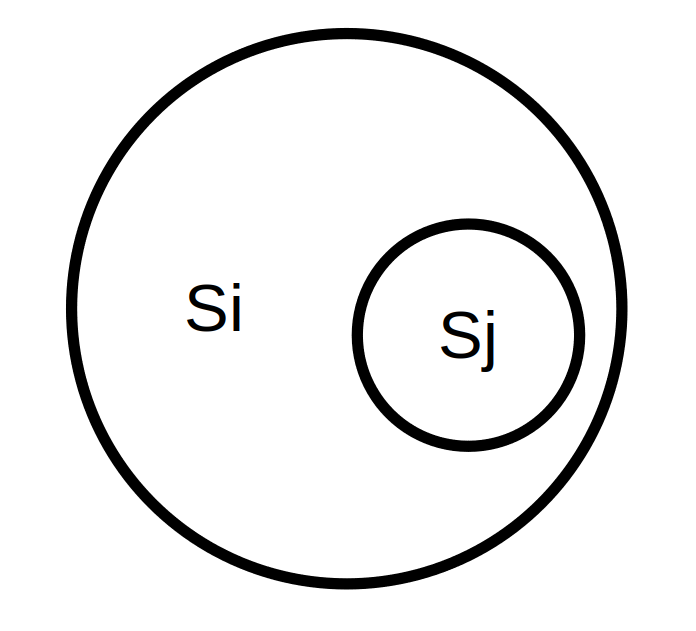
\includegraphics[width=0.4\linewidth]{figures/sd_sets/inclusion2.png}}}

\scnheader{объединение*}
\scnidtf{объединение множеств*}
\scniselement{квазибинарное отношение}
\scniselement{ориентированное отношение}
\scntext{определение}{\textbf{\textit{объединение*}} – это \textit{квазибинарное ориентированное отношение}, областью определения которого является семейство всевозможных множеств. Будем говорить, что \textit{Множество Si} является объединением \textit{Множество Sj} и \textit{Множество Sk} тогда и только тогда, когда любой элемент \textit{Множество Si} является элементом или \textit{Множество Sj} или \textit{Множество Sk}.}
\scnrelfrom{описание примера}{
\scnfilescg {figures/sd_sets/union.png}}
\scnaddlevel{1}
\scnexplanation{Множество \textit{Si} является объединением множеств \textit{Sj}, \textit{Sk} и \textit{Sm}.}
\scnaddlevel{-1}
\scnrelfrom{изображение}{
\scnfileimage{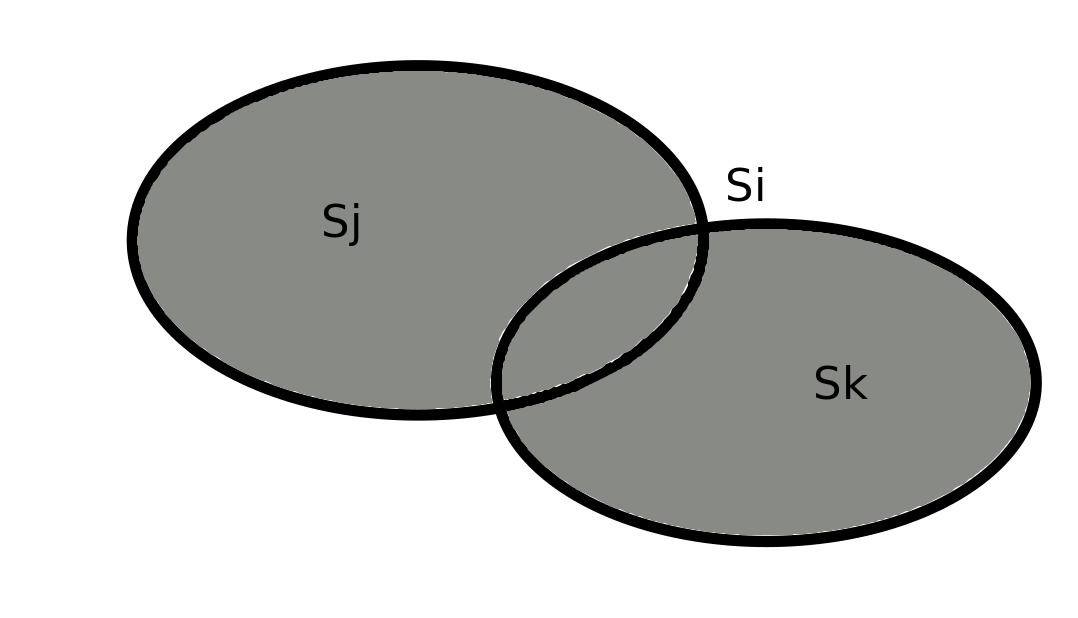
\includegraphics[width=0.6\linewidth]{figures/sd_sets/union2.png}}}

\scnheader{разбиение*}
\scnidtf{разбиение  множества*}
\scnidtf{объединение попарно непересекающихся множеств*}
\scnidtf{декомпозиция множества*}
\scniselement{квазибинарное отношение}
\scniselement{ориентированное отношение}
\scniselement{отношение декомпозиции}
\scntext{определение}{\textbf{\textit{разбиение*}} – это \textit{квазибинарное ориентированное отношение}, областью определения которого является семейство всевозможных множеств. В результате разбиения множества получается множество попарно непересекающихся множеств, объединение которых есть исходное множество.\\
Семейство множеств \{\textit{S1…, Sn}\} является разбиением множества \textit{Si} в том и только том случае, если:
\begin{scnitemize}
    \item семейство \{\textit{S1…, Sn}\} является семейством \textit{попарно непересекающихся множеств};
    \item семейство \{\textit{S1…, Sn}\} является покрытием множества \textit{Si} (или другими словами, множество \textit{Si} является \textit{объединением} множеств, входящих в указанное выше семейство)
\end{scnitemize}
}
\scnrelfrom{описание примера}{
\scnfilescg{figures/sd_sets/split.png}}
\scnaddlevel{1}
\scnexplanation{Множество \textit{Si} разбивается на множества \textit{Sj}, \textit{Sk} и \textit{Sm}.}
\scnaddlevel{-1}
\scnrelfrom{изображение}{
\scnfileimage{\includegraphics[width=0.5\linewidth]{figures/sd_sets/split2.png}}}

\scnheader{пересечение*}
\scnidtf{пересечение множеств*}
\scniselement{квазибинарное отношение}
\scniselement{ориентированное отношение}
\scntext{определение}{\textbf{\textit{пересечение*}} – это операция над множествами, аргументами которой являются два или большее число множеств, а результатом является множество, элементами которого являются все те и только те сущности, которые одновременно принадлежат каждому множеству, которое входит в семейство аргументов этой операции.\\
Будем говорить, что \textit{Множество Si} является пересечением \textit{Множество Sj} и \textit{Множество Sk} тогда и только тогда, когда любой элемент \textit{Множество Si} является элементом \textit{Множество Sj} и элементом \textit{Множество Sk}.}
\scnrelfrom{описание примера}{
\scnfilescg{figures/sd_sets/intersection.png}}
\scnaddlevel{1}
\scnexplanation{Множество \textit{Si} является результатом пересечения множеств \textit{Sj}, \textit{Sk} и \textit{Sm}.}
\scnaddlevel{-1}
\scnrelfrom{изображение}{
\scnfileimage{\includegraphics[width=0.5\linewidth]{figures/sd_sets/intersection2.png}}}

\scnheader{пара пересекающихся множеств*}
\scniselement{бинарное отношение}
\scniselement{неориентированное отношение}
\scnexplanation{\textbf{\textit{пара пересекающихся множеств*}} – \textit{бинарное неориентированное отношение} между двумя \textit{множествами}, имеющими непустое \textit{пересечение*}.}
\scntext{определение}{\textbf{\textit{пара пересекающихся множеств*}} – \textit{бинарное неориентированное отношение} между двумя \textit{множествами}, имеющими, по крайней мере, один общий для этих двух множеств элемент.}
\scnrelfrom{описание примера}{
\scnfilescg{figures/sd_sets/pairOfIntersectingSets.png}}
\scnaddlevel{1}
\scnexplanation{Множество \textit{Si} и множество \textit{Sj} являются парой пересекающихся множеств.}
\scnaddlevel{-1}
\scnrelfrom{изображение}{
\scnfileimage{\includegraphics[width=0.5\linewidth]{figures/sd_sets/pairOfIntersectingSets2.png}}}

\scnheader{попарно пересекающиеся множества*}
\scnidtf{семейство попарно пересекающихся множеств*}
\scnsuperset{пересекающиеся множества*}
\scniselement{отношение}
\scntext{определение}{\textbf{\textit{попарно пересекающиеся множества*}} – семейство множеств, каждая пара которых является парой пересекающихся множеств, т.е. каждая пара которых имеет хотя бы один общий элемент}
\scntext{примечание}{Не каждое \textit{семейство попарно пересекающихся множеств*} является \textit{семейством пересекающихся множеств*}, хотя обратное верно.}
\scnrelfrom{изображение}{
\scnfilescg{figures/sd_sets/pairwiseIntersectingSets.png}}
\scnaddlevel{1}
\scnexplanation{Множества \textit{Si}, \textit{Sj}, \textit{Sk} и \textit{Sl} являются попарно пересекающимися множествами.}
\scnaddlevel{-1}
\scnrelfrom{изображение}{
\scnfileimage{\includegraphics[width=0.7\linewidth]{figures/sd_sets/pairwiseIntersectingSets2.png}}}

\scnheader{пересекающиеся множества*}
\scnidtf{семейство пересекающихся множеств*}
\scnidtf{быть семейством пересекающихся множеств*}
\scnidtf{семейство множеств, имеющих по крайней мере один элемент, являющийся общим для всех этих множеств*}
\scnsuperset{попарно пересекающиеся множества*}
\scntext{определение}{\textbf{\textit{пересекающиеся множества*}} – это семейство множеств, имеющих по крайней мере один общий для всех этих множеств элемент}
\scnrelfrom{описание примера}{
\scnfilescg{figures/sd_sets/intersectingSets.png}}
\scnaddlevel{1}
\scnexplanation{Множества \textit{Si}, \textit{Sj}, \textit{Sk} и \textit{Sl} являются пересекающимися множествами.}
\scnaddlevel{-1}

\scnheader{пара непересекающихся множеств*}
\scniselement{бинарное отношение}
\scniselement{неориентированное отношение}
\scntext{определение}{\textbf{\textit{пара непересекающихся множеств*}} – это \textit{бинарное неориентированное отношение} между \textit{множествами}, результатом \textit{пересечения*} которых есть пустое множество.}
\scnrelfrom{описание примера}{
\scnfilescg{figures/sd_sets/pairOfNonIntersectingSets.png}}
\scnaddlevel{1}
\scnexplanation{Множества \textit{Si} и \textit{Sj} являются парой непересекающихся множеств.}
\scnaddlevel{-1}
\scnrelfrom{изображение}{
\scnfileimage{\includegraphics[width=0.5\linewidth]{figures/sd_sets/pairOfNonIntersectingSets2.png}}}

\scnheader{попарно непересекающиеся множества*}
\scnidtf{семейство попарно непересекающихся множеств*}
\scnsubset{непересекающиеся множества*}
\scntext{определение}{\textbf{\textit{попарно непересекающиеся множества*}} – семейство множеств, каждая пара которых является парой непересекающихся множеств, т.е. каждая пара которых не имеет ни одного общего элемента}
\scnrelfrom{изображение}{
\scnfilescg{figures/sd_sets/pairwiseNonIntersectingSets.png}}
\scnaddlevel{1}
\scnexplanation{Множества \textit{Si}, \textit{Sj}, \textit{Sk} и \textit{Sl} являются попарно непересекающимися множествами.}
\scnaddlevel{-1}

\scnheader{непересекающиеся множества*}
\scnidtf{семейство непересекающихся множеств*}
\scnidtf{быть семейством непересекающихся множеств*}
\scntext{определение}{\textbf{\textit{непересекающиеся множества*}} – это семейство множеств, не имеющих ни одного общего элемента для всех этих множеств}
\scnrelfrom{изображение}{
\scnfilescg{figures/sd_sets/nonIntersectingSets.png}
\scnexplanation{Множества \textit{Si}, \textit{Sj}, \textit{Sk} и \textit{Sl} являются непересекающимися множествами.}}

\scnheader{разность множеств*}
\scniselement{бинарное отношение}
\scniselement{ориентированное отношение}
\scntext{определение}{\textbf{\textit{разность множеств*}} – это \textit{бинарное ориентированное отношение}, связывающее между собой \textit{ориентированную пару}, первым элементом которой является уменьшаемое множество, вторым - вычитаемое множество, и множество, являющееся результатом вычитания вычитаемого из уменьшаемого, в которое входят все элементы первого множества, не входящие во второе множество.}
\scnrelfrom{описание примера}{
\scnfilescg{figures/sd_sets/setDifference.png}}
\scnaddlevel{1}
\scnexplanation{Множество \textit{Si} является результатом разности множеств \textit{Sj} и \textit{Sk}.}
\scnaddlevel{-1}
\scnrelfrom{изображение}{\scnfileimage{\includegraphics[width=0.5\linewidth]{figures/sd_sets/setDifference2.png}}}

\scnheader{симметрическая разность множеств*}
\scniselement{бинарное отношение}
\scniselement{ориентированное отношение}
\scntext{определение}{\textbf{\textit{симметрическая разность множеств*}} – это \textit{бинарное ориентированное отношение}, связывающее между собой \textit{пару} множеств и множество, являющееся результатом симметрической разности элементов указанной пары. Будем называть \textit{Множество Si} результатом симметрической разности \textit{Множества Sj} и \textit{Множества Sk} тогда и только тогда, когда любой элемент \textit{Множества Si} является или элементом \textit{Множества Sj} или \textit{Множества Sk}, но не является элементом обоих множеств.}
\scnrelfrom{описание примера}{
\scnfilescg{figures/sd_sets/symmetricDifferenceOfSets.png}
\scnexplanation{Множество \textit{Si} является результатом симметрической разности множеств \textit{Sj} и \textit{Sk}.}}
\scnrelfrom{изображение}{
\scnfileimage{\includegraphics[width=0.5\linewidth]{figures/sd_sets/symmetricDifferenceOfSets2.png}}}

\scnheader{декартово произведение*}
\scnidtf{декартово произведение множеств*}
\scnidtf{прямое произведение множеств*}
\scniselement{бинарное отношение}
\scniselement{ориентированное отношение}
\scntext{определение}{\textbf{\textit{декартово произведение*}} – это \textit{бинарное ориентированное отношение} между \textit{ориентированной парой} множеств и \textit{множеством}, элементами которого являются всевозможные упорядоченные пары, первыми элементами которых являются элементы первого из указанных множеств, вторыми – элементы второго из указанных множеств.}
\scnrelfrom{описание примера}{
\scnfilescg{figures/sd_sets/cartesianMultiplication.png}}
\scnaddlevel{1}
\scnexplanation{Множество \textit{Si} является результатом декартова произведения множеств \textit{Sj} и \textit{Sk}.}
\scnaddlevel{-1}

\scnheader{декартово произведение}
\scnidtf{второй домен отношения быть декартовым произведением}
\scnrelfrom{второй домен}{декартово произведение*}

\scnheader{семейство подмножеств*}
\scnidtf{семейство подмножеств заданного множества*}
\scniselement{бинарное отношение}
\scniselement{ориентированное отношение}
\scnsuperset{булеан*}
\scntext{определение}{\textbf{\textit{семейство подмножеств*}} – это \textit{бинарное ориентированное отношение} между множеством и некоторым семейством множеств, каждое из которых является подмножеством первого множества.}
\scnrelfrom{описание примера}{
\scnfilescg{figures/sd_sets/familyOfSubsets.png}
}

\scnheader{булеан*}
\scnidtf{булеан множества*}
\scnidtf{семейство всевозможных подмножеств заданного множества*}
\scniselement{бинарное отношение}
\scniselement{ориентированное отношение}
\scntext{определение}{\textbf{\textit{булеан*}} – это \textit{бинарное ориентированное отношение} между множеством и некоторым семейством множеств, каждое из которых является подмножеством первого множества.}
\scnrelfrom{описание примера}{
\scnfilescg{figures/sd_sets/boulean.png}
}

\scnheader{булеан}
\scnidtf{второй домен отношения быть булеаном}
\scnrelfrom{второй домен}{булеан*}

\scnheader{мощность множества}
\scnidtf{кардинальное число}
\scnidtf{общее число вхождений элементов в заданное множество}
\scnidtf{класс эквивалентности, элементами которого являются знаки всех тех и только тех множеств, которые имеют одинаковую мощность}
\scnidtf{класс эквивалентности, соответствующий отношению быть парой множеств, имеющих одинаковую мощность (равномощность множеств)}
\scnidtf{величина мощности множеств}
\scnidtf{трансфинитное число}
\scnidtf{мощность по Кантору}
\scniselement{параметр}
\scnexplanation{\textbf{\textit{мощность множества}} – это \textit{параметр}, элементами которых являются \textit{множества}, имеющие одинаковое количество элементов. Значением данного параметра является числовая величина, задающая количество элементов, входящих в данный класс множеств, т.е. по сути, количество \textit{позитивных sc-дуг принадлежности}, выходящих из данного \textit{множества}.

Для двух множеств, имеющих одинаковую мощность, существует взаимно-однозначное соответствие между ними (между множествами вхождений элементов в эти множества – на случай мультимножеств).}
\scnrelfrom{описание примера}{
\scnfilescg{figures/sd_sets/power.png}
}

\scnheader{равенство множеств*}
\scniselement{бинарное отношение}
\scniselement{неориентированное отношение}
\scnidtf{быть равными множествами*}
\scntext{определение}{\textbf{\textit{равенство множеств}}* - бинарное неориентированное отношение, выражающее отношение равенства множеств.

Любые два множества являются равными множествами тогда и только тогда, когда первое является включением второго и второе является включением первого.}
\scnrelfrom{описание примера}{
\scnfilescg{figures/sd_sets/equalityOfSets.png}}
\scnaddlevel{1}
\scnexplanation{Множество \textit{Si} равно множеству \textit{Sj}.}
\scnaddlevel{-1}

\bigskip
\scnendstruct \scnendcurrentsectioncomment

\end{SCn}

\scsection{Предметная область и онтология связок и отношений}
\label{sec:sd_rels}
\begin{SCn}

\scnsectionheader{\currentname}

\scnstartsubstruct

\scnheader{Предметная область связок и отношений}
\scniselement{предметная область}
\scnsdmainclasssingle{связь}
\scnsdclass{бинарная связь;sc-коннектор;неатомарная бинарная связь;небинарная связь;неориентированная связь;ориентированная связь;отношение;класс равномощных связок;класс связок разной мощности;унарное отношение;бинарное отношение;квазибинарное отношение;тернарное отношение;небинарное отношение;ориентированное отношение;неориентированное отношение;рефлексивное отношение;антирефлексивное отношение;частично рефлексивное отношение;симметричное отношение;антисимметричное отношение;частично симметричное отношение;транзитивное отношение;антитранзитивное отношение;частично транзитивное отношение;связанное отношение;отношение порядка;отношение строгого порядка;отношение нестрогого порядка;отношение толерантности;отношение эквивалентности;ролевое отношение;числовой атрибут;неролевое отношение;неролевое бинарное отношение;арность;метаотношение;отношение декомпозиции;отношение интеграции}
\scnsdrelation{область определения*;атрибут отношения*;домен*;первый домен*;второй домен*;композиция отношений*;фактор-множество*;соответствие*;отношение соответствия*;область отправления';область прибытия’;образ';прообраз';всюду определенное соответствие*;частично определенное соответствие*;сюръективное соответствие*;несюръективное соответствие*;однозначное соответствие*;обратное соответствие*;обратимое соответствие*;неоднозначное соответствие*;инъективное соответствие*;взаимно однозначное соответствие*;множество сочетаний*;множество размещений*;множество перестановок*}

\scnheader{связь}
\scnidtf{связка sc-элементов}
\scnidtf{sc-связка}
\scnexplanation{\textbf{\textit{связь}} – множество, являющееся абстрактной моделью связи между описываемыми сущностями, которые или знаки которых являются элементами этого множества.}
\scntext{примечание}{Напомним, что все элементы множества, представленного в SC-коде, являются знаками, но описываемыми сущностями могут быть не только сущности, обозначаемые sc-элементами, но и сами эти sc-элементы.}
\scnsubdividing{бинарная связь;небинарная связь}
\scnsubdividing{неориентированная связь;ориентированная связь}

\scnheader{бинарная связь}
\scnsubdividing{sc-коннектор;неатомарная бинарная связь}
\scntext{примечание}{Данное разбиение осуществляется на основе синтаксического признака, а не семантического, поскольку каждый \textit{sc-коннектор} может быть записан в памяти при помощи семантически эквивалентной конструкции, содержащей знак самой связи и пары принадлежности, ведущие к ее элементам, уточненные, при необходимости ролевыми отношениями.}

\scnheader{sc-коннектор}
\scnidtf{атомарная бинарная связь}
\scnexplanation{Каждый \textbf{\textit{sc-коннектор}} представлен в \textit{sc-памяти} одним \textit{sc-элементом} и семантически эквивалентен конструкции, содержащей знак некоторой \textit{бинарной связи} и пары принадлежности, ведущие к элементам этой связи, уточненные, при необходимости ролевыми отношениями.

Такая конструкция может быть обозначена \textbf{\textit{sc-коннектором}} только в случае, когда роли компонентов соответствующей бинарной связи указываются только при помощи \textit{числовых атрибутов 1’} и \textit{2’} или не уточняются вообще.}

\scnheader{неатомарная бинарная связь}
\scnexplanation{\textbf{\textit{неатомарная бинарная связь}} – \textit{бинарная связь}, роли компонентов которой не могут быть заданы только при помощи \textit{ролевых отношений 1'} и \textit{2'}, или не заданы совсем, а требуют дополнительного уточнения при помощи более частных ролевых отношений.}

\scnheader{небинарная связь}
\scnexplanation{\textbf{\textit{небинарная связь}} – связь, имеющая больше двух элементов.}

\scnheader{неориентированная связь}
\scnsuperset{неориентированное множество}
\scnexplanation{\textbf{\textit{неориентированная связь}} – связь, все элементы которой имеют одинаковые роли (при этом соответствующее ролевое отношение, как правило, явно не указывается).}

\scnheader{ориентированная связь}
\scnsuperset{ориентированное множество}
\scnexplanation{\textbf{\textit{ориентированная связь}} – связь, в которой с помощью ролевых отношений, указываются роли компонентов этой связи.}

\scnheader{отношение}
\scnidtf{класс связей}
\scnidtf{класс sc-связок}
\scnidtf{множество отношений}
\scnidtf{Множество всевозможных отношений}
\scntext{определение}{\textbf{\textit{отношение}}, \textit{заданное на множестве M} – это подмножество \textit{декартового произведения} этого множества самого на себя некоторое количество раз.

В более широком смысле \textbf{\textit{отношение}} – это математическая структура, которая формально определяет свойства различных объектов и их взаимосвязи.}
\scnsubdividing{класс равномощных связок;класс связок разной мощности}
\scnsubdividing{бинарное отношение;небинарное отношение}
\scnsubdividing{ориентированное отношение;неориентированное отношение}
\scnsubdividing{ролевое отношение;неролевое отношение}

\scnheader{класс равномощных связок}
\scnidtf{класс связок фиксированной арности}
\scnidtf{отношение, обладающее свойством арности}
\scnsuperset{унарное отношение}
\scnsuperset{бинарное отношение}
\scnsuperset{тернарное отношение}
\scntext{определение}{\textbf{\textit{класс равномощных связок}} – класс связок, имеющих одинаковую мощность.}

\scnheader{класс связок разной мощности}
\scnidtf{отношение нефиксированной арности}
\scnsubset{небинарное отношение}
\scntext{определение}{\textbf{\textit{класс связок разной мощности}} – класс связок, имеющих разную мощность.}

\scnheader{унарное отношение}
\scnidtf{отношение арности один}
\scnidtf{одноместное отношение}
\scnidtf{множество синглетонов}
\scntext{определение}{\textbf{\textit{унарное отношение}} – это множество таких отношений на множестве M, являющихся любым подмножеством множества M.}

\scnheader{бинарное отношение}
\scnidtf{отношение арности два}
\scnidtf{двухместное отношение}
\scnsuperset{квазибинарное отношение}
\scnsuperset{отношение порядка}
\scnsuperset{отношение толерантности}
\scnsubdividing{рефлексивное отношение;антирефлексивное отношение;частично рефлексивное отношение}
\scnsubdividing{симметричное отношение;антисимметричное отношение;частично симметричное отношение}
\scnsubdividing{транзитивное отношение;антитранзитивное отношение;частично транзитивное отношение}
\scnsubdividing{ролевое отношение;неролевое бинарное отношение}
\scntext{определение}{\textbf{\textit{бинарное отношение}} – это множество таких отношений на множестве \textbf{\textit{M}}, являющихся подмножеством \textit{декартова произведения} множества \textbf{\textit{M}}.\\
Если \textbf{\textit{бинарное отношение R}} задано на \textit{множестве} \textbf{\textit{М}} и два элемента этого множества \textbf{\textit{a}} и \textbf{\textit{b}} связаны данным отношением, то будем обозначать такую связь как \textbf{\textit{aRb}}.}

\scnheader{квазибинарное отношение}
\scnexplanation{\textbf{\textit{квазибинарное отношение}} – множество ориентированных пар, первые компоненты которых являются связками.\\
Таким образом, \textit{sc-дуги}, принадлежащие \textbf{\textit{квазибинарным отношениям}}, всегда выходят из связок.}
\scntext{sc-утверждение}{В область определения квазибинарного отношения будем включать:
\begin{scnitemize}
    \item вторые компоненты ориентированных пар, принадлежащих этому отношению;
    \item элементы первых компонентов ориентированных пар, принадлежащих этому отношению;
    \item других элементов область определения квазибинарного отношения не содержит.
\end{scnitemize}
}

\scnheader{тернарное отношение}
\scnidtf{отношение арности три}
\scnidtf{трехместное отношение}
\scnexplanation{\textbf{\textit{тернарное отношение}} – это множество отношений, связывающих между собой три элемента.}

\scnheader{небинарное отношение}
\scnexplanation{\textbf{\textit{небинарное отношение}} – это множество отношений, хотя бы одна из связок каждого из которых имеет значение мощности больше двух.}

\scnheader{ориентированное отношение}
\scntext{определение}{\textbf{\textit{ориентированное отношение}} – это множество таких отношений, каждая связка которых является ориентированным множеством.}

\scnheader{неориентированное отношение}
\scntext{определение}{\textbf{\textit{неориентированное отношение}} – это множество таких отношений, каждая связка которых является неориентированным множеством.}

\scnheader{рефлексивное отношение}
\scntext{определение}{\textbf{\textit{рефлексивное отношение}} – это \textit{бинарное отношение}, любая пара которого есть канторовское множество.}

\scnheader{антирефлексивное отношение}
\scntext{определение}{\textbf{\textit{антирефлексивное отношение R}} на \textit{множестве} \textbf{\textit{A}} – это \textit{бинарное отношение}, в котором все элементы множества \textbf{\textit{A}} не находятся в отношении \textbf{\textit{R}} к самому себе.}

\scnheader{частично рефлексивное отношение}
\scntext{определение}{\textbf{\textit{частично рефлексивное отношение R}} на \textit{множестве} \textbf{\textit{A}} – это \textit{бинарное отношение},  в котором хотя бы один (но не все) элемент множества \textbf{\textit{A}} находится в отношении \textbf{\textit{R}} к самому себе.}

\scnheader{симметричное отношение}
\scntext{определение}{\textbf{\textit{симметричное отношение R}} на \textit{множестве} \textbf{\textit{A}} – это \textit{бинарное отношение}, в котором для каждой пары элементов \textbf{\textit{а}} и \textbf{\textit{b}} этого множества выполнение отношения \textbf{\textit{aRb}} влечёт выполнение \textbf{\textit{bRa}}.}

\scnheader{антисимметричное отношение}
\scntext{определение}{\textbf{\textit{антисимметричное отношение R}} на \textit{множестве} \textbf{\textit{A}} – это \textit{бинарное отношение}, в котором для каждой пары элементов \textbf{\textit{а}} и \textbf{\textit{b}} этого множества выполнение отношений \textbf{\textit{aRb}} и \textbf{\textit{bRa}} влечёт равенство \textbf{\textit{a}} и \textbf{\textit{b}}.}

\scnheader{частично симметричное отношение}
\scntext{определение}{\textbf{\textit{частично симметричное отношение R}} на \textit{множестве} \textbf{\textit{A}} – это \textit{бинарное отношение}, в котором для каждой пары элементов \textbf{\textit{а}} и \textbf{\textit{b}} (но не для всех таких пар) этого множества выполнение отношения \textbf{\textit{aRb}} влечёт выполнение \textbf{\textit{bRa}}.}

\scnheader{транзитивное отношение}
\scntext{определение}{\textbf{\textit{транзитивное отношение R}} на \textit{множестве} \textbf{\textit{A}} – это \textit{бинарное отношение}, в котором для любых трёх элементов этого множества \textbf{\textit{a, b, c}} выполнение отношений \textbf{\textit{aRb}} и \textbf{\textit{bRc}} влечёт выполнение отношения \textbf{\textit{aRc}}.}

\scnheader{антитранзитивное отношение}
\scntext{определение}{\textbf{\textit{антитранзитивное отношение R}} на \textit{множестве} \textbf{\textit{A}} – это \textit{бинарное отношение}, в котором для любых трёх элементов этого множества \textbf{\textit{a, b, c}} выполнение отношений \textbf{\textit{aRb}} и \textbf{\textit{bRc}} не влечёт выполнение отношения \textbf{\textit{aRc}}.}

\scnheader{частично транзитивное отношение}
\scntext{определение}{\textbf{\textit{частично транзитивное отношение R}} на \textit{множестве} \textbf{\textit{A}} – это \textit{бинарное отношение}, в котором для каждых трёх элементов этого множества \textbf{\textit{a, b, c}} (но не для всех таких троек) выполнение отношений \textbf{\textit{aRb}} и \textbf{\textit{bRc}} влечёт выполнение отношения \textbf{\textit{aRc}}.}

\scnheader{связанное отношение}
\scnsubset{бинарное отношение}
\scntext{определение}{\textbf{\textit{связанное отношение R}} на \textit{множестве} \textbf{\textit{A}} – это \textit{бинарное отношение}, в котором для каждой пары элементов \textbf{\textit{а}} и \textbf{\textit{b}} этого множества выполняется одно из двух отношений: \textbf{\textit{aRb}} или \textbf{\textit{bRa}}.}

\scnheader{отношение порядка}
\scnsubdividing{отношение строгого порядка;отношение нестрогого порядка}
\scntext{определение}{\textbf{\textit{отношение порядка}} – это \textit{бинарное отношение}, обладающее свойством транзитивности и антисимметричности.}

\scnheader{отношение строгого порядка}
\scntext{определение}{\textbf{\textit{отношение строгого порядка}} – это \textit{отношение порядка}, обладающее свойством антирефлексивности.}

\scnheader{отношение нестрогого порядка}
\scntext{определение}{\textbf{\textit{отношение нестрогого порядка}} – это \textit{отношение порядка}, обладающее свойством рефлексивности.}

\scnheader{отношение толерантности}
\scntext{определение}{\textbf{\textit{отношение толерантности}} – это \textit{бинарное отношение}, принадлежащее классам \textit{симметричное отношение} и \textit{рефлексивное отношение}.}

\scnheader{отношение эквивалентности}
\scnidtf{максимальное семейство отношений эквивалентности}
\scnsubset{отношение толерантности}
\scntext{определение}{\textbf{\textit{отношение эквивалентности}} – это \textit{отношение толерантности}, принадлежащее классу \textit{транзитивных отношений}}
\scntext{примечание}{Каждое отношение эквивалентности уточняет то, что мы считаем эквивалентными сущностями, т.е. то, на какие сходства этих сущностей мы обращаем внимание и какие их отличия мы игнорируем (не учитываем).}

\scnheader{ролевое отношение}
\scnidtf{атрибут}
\scnidtf{атрибутивное отношение}
\scnidtf{отношение, которое задает роль элементов в рамках некоторого множества}
\scnidtf{отношение, являющееся подмножеством отношения принадлежности}
\scnrelto{семейство подмножеств}{принадлежность*}
\scnsubset{бинарное отношение}
\scnsuperset{числовой атрибут}
\scnexplanation{\textbf{\textit{ролевое отношение}} – это отношение, являющееся подмножеством отношения принадлежности.}
\scntext{правило идентификации экземпляров}{В конце каждого \textit{идентификатора}, соответствующего экземплярам класса \textbf{\textit{ролевое отношение}}, не являющегося системным, ставится знак «'».

Например:\\
\textit{ключевой экземпляр’}

Из-за ограничений в разрешенном алфавите символов, в системном идентификаторе не может быть использовать знак «'», поэтому в начале каждого \textit{системного идентификатора}, соответствующего экземплярам класса \textbf{\textit{ролевое отношение}} ставится префикс «rrel\_».

Например:\\
\textit{rrel\_key\_sc\_element}}

\scnheader{числовой атрибут}
\scnidtf{порядковый номер}
\scnidtf{номер компонента ориентированной связки}
\scnhaselement{1’; 2’; 3’; 4’; 5’; 6’; 7’; 8’; 9’; 10’}
\scnexplanation{\textbf{\textit{числовой атрибут}} – \textit{ролевое отношение}, задающее порядковый номер элемента некоторой ориентированной связки, не уточняя при этом семантику такой принадлежности. Во многих случаях бывает достаточно использовать числовые атрибуты, чтобы различать компоненты связки, семантика каждого из которых дополнительно оговаривается, например, при определении отношения, которому данная связка принадлежит.}

\scnheader{неролевое отношение}
\scnsubdividing{небинарное отношение;неролевое бинарное отношение}
\scnexplanation{\textbf{\textit{неролевое отношение}} – отношение, не являющееся подмножеством отношения принадлежности.}
\scntext{правило идентификации экземпляров}{В конце каждого \textit{идентификатора}, соответствующего экземплярам класса \textbf{\textit{неролевое отношение}}, не являющегося системным, ставится знак «*».

Например:\\
\textit{включение*}

Из-за ограничений в разрешенном алфавите символов, в системном идентификаторе не может быть использовать знак «*», поэтому в начале каждого \textit{системного идентификатора}, соответствующего экземплярам класса \textbf{\textit{неролевое отношение}} ставится префикс «nrel\_».

Например:\\
\textit{nrel\_inclusion}}

\scnheader{неролевое бинарное отношение}
\scnexplanation{\textbf{\textit{неролевое бинарное отношение}} – \textit{бинарное отношение}, не являющееся \textit{ролевым отношением}.}

\scnheader{арность}
\scnidtf{арность отношения}
\scniselement{параметр}
\scnexplanation{\textbf{\textit{арность}} – это параметр, каждый элемент которого представляет собой класс \textit{отношений}, каждая связка которых имеет одинаковую \textit{мощность}. Значение данного \textit{параметра} совпадает со значением \textit{мощности} каждой из таких связок.}
\scnrelfrom{описание примера}{
\scnfilescg{figures/sd_relations/arity.png}}


\scnheader{область определения*}
\scnidtf{область определения отношения*}
\scniselement{бинарное отношение}
\scnexplanation{\textbf{\textit{область определения*}} – это \textit{бинарное отношение}, связывающее отношение со множеством, являющимся его областью определения.

Областью определения отношения будем называть результат теоретико-множественного объединения всех связок этого отношения, или, другими словами, результат теоретико-множественного объединения всех множеств, являющихся доменами данного отношения.}
\scnrelfrom{описание примера}{
\scnfilescg{figures/sd_relations/domain.png}}

\scnheader{атрибут отношения*}
\scnidtf{ролевой атрибут, используемый в связках заданного отношения*}
\scniselement{бинарное отношение}
\scnexplanation{\textbf{\textit{атрибут отношения*}} – это \textit{бинарное отношение}, связывающее заданное отношение с \textit{ролевым отношением}, используемым в данном отношении для уточнения роли того или иного элемента связок данного отношения.}
\scnrelfrom{описание примера}{
\scnfilescg{figures/sd_relations/relationshipAttribute.png}}


\scnheader{домен*}
\scnidtf{домен отношения по заданному атрибуту*}
\scniselement{бинарное отношение}
\scnexplanation{\textbf{\textit{домен*}} – это \textit{бинарное отношение}, связывающее связку отношения \textit{атрибут отношения*} со множеством, являющимся доменом заданного отношения по заданному атрибуту. Множество \textbf{\textit{di}} является доменом отношения \textbf{\textit{ri}} по атрибуту \textbf{\textit{ai}} в том и только том случае, если элементами этого множества являются все те и только те элементы связок отношения \textbf{\textit{ri}}, которые имеют в рамках этих связок атрибут \textbf{\textit{ai}}.}
\scnrelfrom{описание примера}{
\scnfilescg{figures/sd_relations/domen.png}}


\scnheader{первый домен*}
\scniselement{бинарное отношение}
\scntext{определение}{\textbf{\textit{первый домен*}} – это \textit{бинарное отношение}, связывающее отношение с множеством, являющимся доменом по атрибуту \textbf{\textit {1'}} данного отношения.}
\scnrelfrom{описание примера}{
\scnfilescg{figures/sd_relations/firstDomain.png}}

\scnheader{второй домен*}
\scniselement{бинарное отношение}
\scntext{определение}{\textbf{\textit{второй домен*}} – это \textit{бинарное отношение}, связывающее отношение с множеством, являющимся доменом по атрибуту \textbf{\textit{2'}} данного отношения.}
\scnrelfrom{описание примера}{
\scnfilescg{figures/sd_relations/secondDomain.png}}

\scnheader{композиция отношений*}
\scniselement{квазибинарное отношение}
\scntext{определение}{\textbf{\textit{композиция отношений*}} – это \textit{квазибинарное отношение}, связывающее два бинарных отношения с отношением, являющимся их композицией. Под композицией бинарных отношений \textbf{\textit{R}} и \textbf{\textit{S}} будем понимать множество $\{(x, y) | \exists z(xSz \wedge zRy)\}$}
\scnrelfrom{описание примера}{
\scnfilescg{figures/sd_relations/relationshipComposition.png}}

\scnheader{фактор-множество*}
\scnidtf{быть фактор-множеством*}
\scnidtf{множество всевозможных максимальных множеств из попарно эквивалентных элементов*}
\scnidtf{множество всевозможных классов эквивалентности для заданного отношения эквивалентности*}
\scniselement{бинарное отношение}
\scntext{определение}{\textbf{\textit{фактор множество*}} - это бинарное ориентированное отношение, каждая связка которого связывает некоторое отношение эквивалентности со множеством всех соответствующих этому отношению классов эквивалентности. Каждый такой класс представляет собой максимальное множество сущностей, каждая пара которых принадлежит указанному выше отношению эквивалентности.}
\scnrelfrom{описание примера}{
\scnfilescg{figures/sd_relations/factor_set.png}}

\scnheader{метаотношение}
\scntext{определение}{метаотношение - это \textit{отношение}, в каждой связке которого есть по крайней мере один компонент, являющийся знаком некоторого \textit{отношения}.}

\scnheader{отношение декомпозиции}
\scnhaselement{разбиение*}
\scnhaselement{декомпозиция раздела*}
\scnhaselement{декомпозиция абстрактного объекта*}

\scnheader{отношение интеграции}
\scnhaselement{объединение*}

\scnheader{соответствие*}
\scnidtf{наличие соответствия*}
\scniselement{бинарное отношение}
\scnsubdividing{соответствие между непересекающимися множествами*;соответствие между строго пересекающимися множествами*;соответствие, область отправления и область прибытия которого совпадают*}
\scnsubdividing{всюду определенное соответствие*;частично определенное соответствие*}
\scnsubdividing{сюръекция*;несюръективное соответствие*}
\scnsubdividing{однозначное соответствие*;неоднозначное соответствие*}
\scntext{определение}{\textbf{\textit{соответствие*}} – \textit{бинарное отношение}, заданное на множествах и задающее наличие отношения, в котором участвуют только элементы этих множеств.}
\scnrelfrom{описание примера}{
\scnfilescg{figures/sd_relations/conformity.png}}

\scnheader{отношение соответствия*}
\scniselement{бинарное отношение}
\scntext{определение}{\textbf{\textit{отношение соответствия*}} – \textit{бинарное отношение}, связывающее ориентированную пару множеств, на которых задано \textit{соответствие*} и некоторое подмножество \textit{декартова произведения*} этих \textit{множеств}.}
\scnrelfrom{описание примера}{
\scnfilescg{figures/sd_relations/relationshipConformity.png}}

\scnheader{область отправления'}
\scnidtf{область отправления соответствия’}
\scnidtf{область определения соответствия’}
\scnidtf{первый компонент пары в отношении соответствия’}
\scniselement{ролевое отношение}
\scntext{определение}{\textbf{\textit{область отправления'}} – \textit{ролевое отношение}, указывающее на первый компонент пары в рамках отношения \textit{соответствие*}.}
\scnrelfrom{описание примера}{
\scnfilescg{figures/sd_relations/departureArea.png}}

\scnheader{область прибытия’}
\scnidtf{область прибытия соответствия'}
\scnidtf{область значений соответствия'}
\scniselement{ролевое отношение}
\scntext{определение}{\textbf{\textit{область прибытия’}} – \textit{ролевое отношение}, указывающее на второй компонент пары в рамках отношения \textit{соответствие*}.}
\scnrelfrom{описание примера}{
\scnfilescg{figures/sd_relations/arrivalArea.png}}

\scnheader{образ'}
\scnidtf{образ соответствия’}
\scniselement{ролевое отношение}
\scntext{определение}{\textbf{\textit{образ'}} – \textit{ролевое отношение}, указывающее на второй компонент каждой пары в рамках множества пар, которое является вторым компонентом \textit{отношения соответствия*}.}
\scnrelfrom{описание примера}{
\scnfilescg{figures/sd_relations/form.png}}

\scnheader{прообраз'}
\scnidtf{прообраз соответствия’}
\scniselement{ролевое отношение}
\scntext{определение}{\textbf{\textit{прообраз'}} – \textit{ролевое отношение}, указывающее на первый компонент каждой пары в рамках множества пар, которое является первым компонентом \textit{отношения соответствия*}.}
\scnrelfrom{описание примера}{
\scnfilescg{figures/sd_relations/prototype.png}}

\scnheader{всюду определенное соответствие*}
\scnidtf{полное соответствие*}
\scnidtf{наличие всюду определенного соответствия*}
\scntext{определение}{\textbf{\textit{всюду определенное соответствие*}} – это \textit{соответствие*}, при котором существует \textit{образ’} для каждого элемента \textit{области отправления'} данного \textit{соответствия*}.}
\scnrelfrom{описание примера}{
\scnfilescg{figures/sd_relations/surjection.png}}
\scnrelfrom{изображение}{
\scnfileimage{\includegraphics[width=0.5\linewidth]{figures/sd_relations/surjection2.png}}}


\scnheader{частично определенное соответствие*}
\scnidtf{наличие частично определенного соответствия*}
\scntext{определение}{\textbf{\textit{частично определенное соответствие*}} – это \textit{соответствие*}, при котором существует \textit{образ’} для некоторых, но не всех элементов \textit{области отправления'} данного \textit{соответствия*}.}
\scnrelfrom{описание примера}{
\scnfilescg{figures/sd_relations/partiallyDefinedConformity.png}}
\scnrelfrom{изображение}{
\scnfileimage{\includegraphics[width=0.5\linewidth]{figures/sd_relations/partiallySurjection.png}}}


\scnheader{сюръективное соответствие*}
\scnidtf{наличие сюръективного соответствия*}
\scnidtf{сюръекция*}
\scntext{определение}{\textbf{\textit{сюръективное соответствие*}} – это \textit{соответствие*}, при котором существует \textit{прообраз’} для каждого элемента \textit{области прибытия'} данного \textit{соответствия*}.}
\scnrelfrom{описание примера}{
\scnfilescg{figures/sd_relations/surjectiveConformity.png}}
\scnrelfrom{изображение}{
\scnfileimage{\includegraphics[width=0.5\linewidth]{figures/sd_relations/surjectiveConformity2.png}}}

\scnheader{несюръективное соответствие*}
\scnidtf{наличие несюръективного соответствия*}
\scntext{определение}{\textbf{\textit{несюръективное соответствие*}} – это \textit{соответствие*}, при котором не для каждого элемента \textit{области прибытия'} данного \textit{соответствия*} существует \textit{прообраз’}.}
\scnrelfrom{описание примера}{
\scnfilescg{figures/sd_relations/nonSurjectiveConformity.png}}
\scnrelfrom{изображение}{
\scnfileimage{\includegraphics[width=0.5\linewidth]{figures/sd_relations/nonSurjectiveConformity2.png}}}

\scnheader{однозначное соответствие*}
\scnidtf{наличие однозначного соответствия*}
\scnidtf{функциональное соответветствие*}
\scnidtf{функция*}
\scntext{определение}{\textbf{\textit{однозначное соответствие*}} – это \textit{соответствие*}, при котором каждому элементу из \textit{области отправления'} соответствия ставится не более, чем один элемент из \textit{области прибытия’} соответствия.}
\scnrelfrom{описание примера}{
\scnfilescg{figures/sd_relations/singleConformity.png}}
\scnrelfrom{изображение}{
\scnfileimage{\includegraphics[width=0.5\linewidth]{figures/sd_relations/singleConformity2.png}}}

\scnheader{обратное соответствие*}
\scniselement{бинарное отношение}
\scnrelfrom{область определения}{соответствие*}
\scntext{определение}{\textbf{\textit{обратное соответствие*}} – \textit{бинарное отношение}, связывающее два \textit{соответствия*}, при этом выполняются следующие условия:
\begin{scnitemize}
    \item \textit{область отправления’} первого соответствия является \textit{областью прибытия'} второго;
    \item \textit{область прибытия’} первого соответствия является \textit{областью отправления'} второго;
    \item для каждой пары, входящей в состав отношения первого соответствия, существует пара, входящая в состав отношения второго соответствия, при этом \textit{образ’} и \textit{прообраз'} в рамках первой указанной пары являются соответственно \textit{прообразом'} и \textit{образом’} в рамках второй.
\end{scnitemize}
}

\scnheader{обратимое соответствие*}
\scnsubset{однозначное соответствие*}
\scntext{определение}{\textbf{\textit{обратимое соответствие*}} – такое \textit{однозначное соответствие*}, для которого \textit{обратное соответствие*} также является \textit{однозначным соответствием*}.}

\scnheader{неоднозначное соответствие*}
\scntext{определение}{\textbf{\textit{неоднозначное соответствие*}} – это \textit{соответствие*}, при котором хотя бы одному элементу из \textit{области отправления’} соответствия ставится более, чем один элемент из \textit{области прибытия'} соответствия.}
\scnrelfrom{описание примера}{
\scnfilescg{figures/sd_relations/nonSingleConformity.png}}
\scnrelfrom{изображение}{
\scnfileimage{\includegraphics[width=0.5\linewidth]{figures/sd_relations/nonSingleConformity2.png}}}

\scnheader{инъективное соответствие*}
\scnidtf{инъекция*}
\scnsubset{однозначное соответствие*}
\scntext{определение}{\textbf{\textit{инъективное соответствие*}} – это \textit{соответствие*}, при котором разным элементам из \textit{области отправления’} соответствия всегда соответствуют разные элементы из \textit{области прибытия'} соответствия и наоборот.}
\scnrelfrom{описание примера}{
\scnfilescg{figures/sd_relations/injectiveConformity.png}}
\scnrelfrom{изображение}{
\scnfileimage{\includegraphics[width=0.5\linewidth]{figures/sd_relations/injectiveConformity2.png}}}

\scnheader{взаимно однозначное соответствие*}
\scnidtf{биекция*}
\scnsubset{всюду определенное соответствие*}
\scnsubset{сюръективное соответствие*}
\scnsubset{инъективное соответствие*}
\scntext{определение}{\textbf{\textit{взаимно однозначное соответствие*}} – это \textit{инъективное соответствие*}, являющееся всюду определенным и сюръективным.}
\scnrelfrom{описание примера}{
\scnfilescg{figures/sd_relations/bijectiveConformity.png}}
\scnrelfrom{изображение}{
\scnfileimage{\includegraphics[width=0.5\linewidth]{figures/sd_relations/bijectiveConformity2.png}}}


\scnheader{множество сочетаний*}
\scnidtf{множество всевозможных сочетаний*}
\scnidtf{множество всевозможных сочетаний заданной арности из элементов заданного множества*}
\scnidtf{множество всех неориентированных связок заданной арности*}
\scnidtf{множество всех подмножеств заданной мощности*}
\scnidtf{семейство всевозможных сочетаний*}
\scntext{определение}{\textbf{\textit{множество сочетаний*}} - \textit{отношение}, связывающее некоторое множество и семейство всевозможных множеств, имеющих значение мощности, меньше либо равное мощности исходного множества и состоящих из тех же элементов, что и это множество.}
\scntext{утверждение}{Мощность \textbf{\textit{множества сочетаний*}} может быть вычислена как n!/(k!(n-k)!), где \textbf{\textit{n}} – мощность исходного множества, \textbf{\textit{k}} – мощность элементов множества сочетаний.}
\scnrelfrom{описание примера}{
\scnfilescg{figures/sd_relations/setsOfCombinations.png}
\scnexplanation{Для Множества \textbf{\textit{Si}} представлено множество сочетаний по 2 элемента.}}

\scnheader{множество размещений*}
\scntext{определение}{\textbf{\textit{множество размещений*}} - \textit{отношение}, связывающее некоторое множество и семейство всевозможных кортежей, имеющих значение мощности, меньше либо равное мощности исходного множества и состоящих из тех же элементов, что и это множество.}
\scntext{утверждение}{Мощность \textbf{\textit{множества размещений*}} может быть вычислена как n!/(n-k)!, где \textbf{\textit{n}} – мощность исходного множества, \textbf{\textit{k}} – мощность элементов множества сочетаний.}
\scnrelfrom{описание примера}{
\scnfilescg{figures/sd_relations/setsOfPlacements.png}
\scnexplanation{Для Множества \textbf{\textit{Si}} представлено множество размещений по 2 элемента.}}

\scnheader{множество перестановок*}
\scnsubset{множество размещений*}
\scntext{определение}{\textbf{\textit{множество перестановок*}} - \textit{отношение}, связывающее некоторое множество и семейство всевозможных кортежей, равномощных исходному множеству и состоящих из тех же элементов, что и это множество.}
\scntext{утверждение}{Мощность \textbf{\textit{множества перестановок*}} может быть вычислена как n!, где \textbf{\textit{n}} – мощность исходного множества.}
\scnrelfrom{описание примера}{
\scnfilescg{figures/sd_relations/setsOfPermutations.png}
\scnexplanation{Для Множества \textbf{\textit{Si}} представлено его множество перестановок.}}

\scnendstruct \scnendcurrentsectioncomment

\end{SCn}

\scsection{Предметная область и онтология параметров, величин и шкал}
\label{sec:sd_params}
\begin{SCn}

\scnsectionheader{\currentname}

\scnstartsubstruct

\scnheader{Предметная область параметров, величин и шкал}
\scnidtf{Предметная область параметров и классов эквивалентности, являющихся их элементами (значениями, величинами)}
\scniselement{предметная область}
\scnsdmainclasssingle{параметр}
\scnsdclass{измеряемый параметр;неизмеряемый параметр;уровень класса эквивалентности;величина;точная величина;неточная величина;интервальная величина;параметрическая модель;измерение с фиксированной единицей измерения ;измерение по шкале;арифметическое выражение на величинах;арифметическая операция на величинах;действие. измерение;задача. измерение}
\scnsdrelation{область определения параметра*;эталон';измерение*;точность*;единица измерения*;нулевая отметка*;единичная отметка*;сумма величин*;произведение величин*;возведение величин в степень*;большая величина*;равенство величин*;большая или равная величина*}

\scnheader{параметр}
\scnidtf{характеристика}
\scnidtf{свойство}
\scnidtf{признак}
\scnidtf{класс классов}
\scnidtf{измеряемое свойство}
\scnidtf{признак классификации или покрытия некоторого класса сущностей}
\scnidtf{признак разбиения или покрытия некоторого класса сущностей}
\scnidtf{семейство множеств, разбивающих или покрывающих некоторый класс сущностей}
\scnidtf{семейство классов сущностей, обладающих одинаковым соответствующим свойством}
\scnidtf{фактор-множество, соответствующее некоторому отношению эквивалентности, или аналог фактор-множества, соответствующий некоторому отношению толерантности}
\scnsubdividing{измеряемый параметр;неизмеряемый параметр}
\scnexplanation{Каждый \textbf{\textit{параметр}} представляет собой класс, являющийся семейством всевозможных классов эквивалентности или толерантности, задаваемых либо \textit{отношением эквивалентности}, либо \textit{отношением толерантности} (симметричным, рефлексивным, но частично транзитивным). Так, например, элементами (значениями, величинами) \textbf{\textit{параметра}} \textit{длина} являются либо классы эквивалентности, задаваемые отношением эквивалентности «иметь точно одинаковую длину*», либо классы толерантности, задаваемые отношением вида «иметь приблизительно одинаковую длину с указываемой точностью*», либо интервальные классы, задаваемые бинарными отношениями вида «иметь длину, находящуюся в одном и том же указываемом интервале*» (например, от 1 метра до 2 метров).\\
Примерами параметров как отношений эквивалентности являются:
\begin{scnitemize}
    \item равновеликость геометрических фигур (по длине, площади, объему – в зависимости от размерности этих фигур);
    \item иметь одинаковый цвет (быть эквивалентными по цвету);
    \item эквивалентность, по вкусу, запаху, твердости и т.д.
\end{scnitemize}

Заметим, что среди элементов (значений, величин) параметра могут встречаться пересекающиеся множества (классы), но объединение всех элементов каждого параметра есть не что иное, как класс всевозможных сущностей, обладающих этим параметром (свойством, характеристикой). Например, класс всех сущностей, имеющих длину, класс всех сущностей, обладающих цветом.

Каждый конкретный параметр (характеристика), т.е. каждый элемент класса всевозможных параметров (характеристик) есть, по сути, признак классификации сущностей, обладающих это характеристикой, по принципу эквивалентности (одинаковости значения) этой характеристики. Например, параметр \textit{цвет} разбивает множество сущностей имеющих цвет на классы, каждый из которых включает в себя сущности, имеющие одинаковый цвет. Параметр может разбиваться на классы для уточнения некоторого свойства, например элементами параметра цвет будут классы, соответствующие конкретным цветам (синий, красный и т.д.), в свою очередь каждый конкретный цвет может включать более частные классы, уточняющие данное свойство, например, темно-синий, светло-красный и т.д.

Другими словами, каждому множеству сущностей может ставиться в соответствие набор (семейство) параметров (параметрическое пространство), которыми обладают сущности этого множества – аналог семейства отношений, определенных (заданных) на этом множестве. Часто бывает важно построить такое параметрическое пространство, «точки» которого взаимно-однозначно соответствуют параметризуемым сущностям (например, набор параметров, позволяющих однозначно идентифицировать, установить личность каждого человека). 

Таким образом, для каждого используемого элемента (значения) какого-либо параметра, необходимо явно указывать спецификацию этого значения (точное значение, неточное значение, интервальное значение, точность, интервал).}
\scnrelfrom{описание примера}{
\scnfilescg{figures/sd_parameters_and_quantities/parameterDescription.png}
}

\scnheader{область определения параметра*}
\scnidtf{множество всех тех и только тех сущностей, которые являются компонентами значений заданного параметра*}
\scnidtf{множество всех тех и только тех сущностей, которые обладают заданным параметром*}
\scnrelto{включение}{объединение*}

\scnheader{измеряемый параметр}
\scnidtf{количественный параметр}
\scnidtf{семейство измеряемых величин}
\scnidtf{семейство классов эквивалентности, каждому из которых может быть поставлено в соответствие числовое значение}
\scnexplanation{Каждый \textbf{\textit{измеряемый параметр}} представляет собой \textit{параметр}, значение (элемент, экземпляр) которого трактуется как \textit{величина}, которой можно поставить в соответствие ее числовое значение на основании выбранной единицы измерения и точки отсчета (нулевой отметки выбранной шкалы).}

\scnheader{неизмеряемый параметр}
\scnidtf{качественный параметр}

\scnheader{уровень класса эквивалентности}
\scnidtf{уровень параметра}
\scniselement{параметр}
\scnexplanation{Параметр \textbf{\textit{уровень класса эквивалентности}} задает уровень некоторого значения некоторого \textit{параметра} в иерархии значений этого параметра. Уровень класса эквивалентности равен 1, если значение параметра не является частным по отношению к другому значению этого параметра, равен 2, если значение параметра является частным по отношению к значению этого параметра с уровнем 1 и т.д.}
\scnrelfrom{описание примера}{
\scnfilescg{figures/sd_parameters_and_quantities/color.png}
}

\scnheader{величина}
\scnidtf{значение количественного параметра}
\scnidtf{значение измеряемого параметра}
\scnidtf{класс сущностей, имеющих одинаковое значение соответствующего параметра}
\scnrelfromlist{включение}{точная величина;неточная величина;интервальная величина}
\scnexplanation{Каждая \textbf{\textit{величина}} представляет собой однозначный и независящий от шкалы измерения результат измерения некоторой характеристики у некоторой сущности.

Каждой \textbf{\textit{величине}} можно поставить в соответствие ее числовое значение на основании выбранной единицы измерения и точки отсчета (нулевой отметки выбранной шкалы, в случае, если измерение осуществляется по шкале).

Нельзя путать значение параметра (\textbf{\textit{величину}}) и значение величины по некоторой шкале, которое может быть скалярным и векторным.}

\scnheader{точная величина}
\scnidtf{точное значение параметра}
\scnidtf{множество всех точных значений параметра}
\scnidtf{значение параметра, являющееся семейством классов эквивалентности, соответствующим некоторому отношению эквивалентности}
\scnidtf{класс эквивалентности}
\scnexplanation{Каждая \textbf{\textit{точная величина}} имеет одно фиксированное значение в некоторой единице измерения или по какой-либо шкале. При этом считается, что все элементы такого класса имеют одинаковое значение данного параметра и отклонениями можно пренебречь.

Каждой \textbf{\textit{точной величине}} можно поставить в соответствие группу \textit{неточных величин}, являющихся не разбиениями, а покрытиями того же множества, но с разной степенью точности.}
\scnrelfrom{описание примера}{
\scnfilescg{figures/sd_parameters_and_quantities/exactLength.png}
\scnexplanation{В данном примере \textbf{\textit{ki}} обозначает класс сущностей, имеющих длину ровно 5 метров. Конкретный пример такой сущности - \textbf{\textit{bi}}.}}

\scnheader{неточная величина}
\scnidtf{множество неточных значений параметра}
\scnidtf{приблизительная величина}
\scnidtf{приблизительное значение параметра}
\scnidtf{значение параметра в интервале с нефиксированными границами}
\scnexplanation{Каждой \textbf{\textit{неточной величине}} ставится в соответствие ее значение в некоторой единице измерения или по какой-либо шкале, а также дополнительно указывается \textit{точность*}, т.е. возможное отклонение от данного значения.}
\scnrelfrom{описание примера}{
\scnfilescg{figures/sd_parameters_and_quantities/approximateLength.png}
\scnexplanation{В данном примере \textbf{\textit{ki}} обозначает класс сущностей, имеющих длину примерно 25 метров, при этом максимально возможное отклонение от этого значения составляет \textbf{\textit{kj}}, то есть 2 метра. Конкретный пример такой сущности - \textbf{\textit{bi}}.}}

\scnheader{интервальная  величина}
\scnidtf{интервальное значение параметра}
\scnidtf{значение параметра в интервале с фиксированными границами}
\scnidtf{интервал значения параметра из множества пересекающихся интервалов разной длины, имеющих нефиксированные границы}
\scnexplanation{Каждая \textbf{\textit{интервальная величина}} представляет собой класс сущностей, находящихся в рамках точно заданного интервала, минимальная и максимальная точка которого являются \textit{точными величинами}. Результатом \textit{измерения*} такой величины является ориентированная пара, первым компонентом которой является левая (меньшая) граница интервала, вторым компонентом – правая (большая) граница интервала.}
\scnrelfrom{описание примера}{
\scnfilescg{figures/sd_parameters_and_quantities/intervalLength.png}
\scnexplanation{В данном примере \textbf{\textit{ki}} обозначает класс сущностей, имеющих длину, которая лежит в интервале от \textbf{\textit{kj}} до \textit{kl}, то есть в интервале от 4 до 5 метров, а \textbf{\textit{bi}} – конкретный пример такой сущности.}}

\scnheader{эталон'}
\scnidtf{образец'}
\scniselement{ролевое отношение}
\scnexplanation{Ролевое отношение \textit{эталон'} указывает на тот элемент значения некоторого параметра, который в рамках данного класса эквивалентности считается эталонным, то есть он используется как образец при определении данного параметра.

\textit{эталон'} может задаваться как для измеряемых, так и для неизмеряемых параметров, например, эталон метра или эталон красоты.}

\scnheader{измерение*}
\scnidtf{значение параметра*}
\scnidtf{значение величины*}
\scnidtf{измерение как соответствие*}
\scnidtf{результат измерения заданной величины в заданной единице измерения и по заданной шкале*}
\scnidtf{бинарное ориентированное отношение, связывающее различные величины с результатами их измерения в различных единицах измерения и по различным шкалам*}
\scnexplanation{Связки отношения \textit{измерение*} связывают величину и ее значение в некоторой единице измерения (в том числе, в интервале) или по некоторой шкале. Конкретная единица измерения или шкала указывается дополнительно при помощи соответствующего отношения. Одной величине может соответствовать только одно значение в каждой возможной единице измерения или одна точка на некоторой шкале.}

\scnheader{точность*}
\scnidtf{отклонение*}
\scnidtf{степень точности неточного значения параметра*}
\scniselement{бинарное отношение}
\scnexplanation{Связки отношения \textbf{\textit{точность*}} связывают \textit{неточную величину} и \textit{точную величину} того же класса, задающую максимальное возможное отклонение указанной \textit{неточной величины} от своего значения.}

\scnheader{параметрическая модель}
\scnidtf{параметрическая спецификация}
\scnidtf{параметрическое sc-описание заданной сущности}
\scnidtf{описание сущности как точки в некотором параметрическом (признаковом) пространстве}
\scnrelto{включение}{семантическая окрестность}
\scnexplanation{Каждая \textbf{\textit{параметрическая модель}} представляет собой описание заданной сущности в некотором параметрическом пространстве количественных и качественных \textit{параметров}, т.е. указание того, какие значения заданных параметров (характеристик) соответствуют описываемой (заданной) сущности.}

\scnheader{единица измерения*}
\scniselement{бинарное отношение}
\scnexplanation{Связки отношения \textbf{\textit{единица измерения*}} связывают знак конкретного \textbf{\textit{измерения с фиксированной единицей измерения}} и некоторую \textit{точную величину}, входящую в тот же конкретный \textit{параметр}, что и первый компонент связок этого конкретного измерения, и которая используется в данном случае в качестве единицы измерения.}

\scnheader{измерение с фиксированной единицей измерения }
\scnrelto{семейство подмножеств}{измерение*}
\scnexplanation{Каждая \textbf{\textit{измерение с фиксированной единицей измерения}} представляет собой подмножество отношения \textit{измерение*} и характеризуется некоторой \textit{единицей измерения*}, которая является элементом того же параметра (семейством сущностей, имеющих значение данного параметра, совпадающее с этой единицей измерения).}

\scnheader{измерение по шкале}
\scnidtf{шкала}
\scnrelto{семейство подмножеств}{измерение*}
\scnexplanation{Каждая \textbf{\textit{измерение по шкале}} представляет собой подмножество отношения \textit{измерение*} и характеризуется не единицей измерения, а некоторой точкой отсчета для данной \textbf{\textit{шкалы}}. Результатом \textbf{\textit{измерения по шкале}} будет некоторая точка шкалы, отстоящая от точки отсчета на определенное расстояние в нужную сторону (меньшую или большую). Понятно, что это расстояние может быть измерено любыми единицами измерения, но его величина при этом останется неизменной.

Не стоит путать измерение по \textbf{\textit{измерение по шкале}}, которое зависит от \textit{нулевой отметки*}, с измерением изменения того же \textit{параметра}, которое характеризуется единицей измерения и не зависит от точки отсчета. Например, не стоит путать дату по некоторому календарю, соответствующую \textit{началу} какого-либо процесса, и \textit{длительность} этого процесса, которая не зависит от выбранного календаря.}
\scnrelfrom{описание примера}{
\scnfilescg{figures/sd_parameters_and_quantities/scale.png}
\scnexplanation{В данном примере \textbf{\textit{ki}} обозначает класс сущностей, имеющих точную температуру в 330 К, а \textbf{\textit{bi}} – конкретный пример такой сущности.}}

\scnheader{нулевая отметка*}
\scnidtf{нуль по шкале*}
\scnidtf{начало отсчета*}
\scniselement{бинарное отношение}
\scnexplanation{Связки отношения \textbf{\textit{нулевая отметка*}} связывают знак некоторого \textit{измерения по шкале} со знаком \textit{точной величины} того же \textit{параметра}, которая в рамках данной шкалы принимается за точку отсчета.}

\scnheader{единичная отметка*}
\scnidtf{единица по шкале*}
\scniselement{бинарное отношение}
\scnexplanation{Связки отношения \textbf{\textit{единичная отметка*}} связывают знак некоторого \textit{измерения по шкале} со знаком \textit{точной величины} того же \textit{параметра}, которая в рамках данной шкалы принимается за единичную отметку, т.е. отметку шкалы, отстоящую от нулевой на расстояние, равное выбранной единице измерения. Вместо указания единичной отметки можно использовать указание единицы измерения, однако величина, выбранная в качестве единицы измерения в этом случае будет принадлежать другому измеряемому параметру, характеризующему \uline{изменение} значения величины параметра, измеряемого по шкале.}

\scnheader{арифметическое выражение на величинах}
\scnexplanation{Каждое \textbf{\textit{арифметическое выражение на величинах}} представляет собой \textit{связку}, компонентами которой являются элементы или подмножества некоторого \textit{количественного параметра}.}

\scnheader{арифметическая операция на величинах}
\scnrelto{семейство подмножеств}{арифметическое выражение на величинах}
\scnexplanation{Каждая \textbf{\textit{арифметическая операция на величинах}} представляет собой \textit{отношение}, элементами которого являются \textit{арифметические выражения на величинах}, то есть множество \textit{арифметических выражений на величинах} какого-либо одного вида.}

\scnheader{сумма величин*}
\scnidtf{сложение величин*}
\scniselement{арифметическая операция на величинах}
\scniselement{квазибинарное отношение}
\scnexplanation{\textbf{\textit{сумма величин*}} – это \textit{арифметическая операция на величинах}, аналогичная \textit{арифметической операции сумма*} для \textit{чисел}.

Первым компонентом связки отношения \textbf{\textit{сумма величин*}} является подмножество некоторого \textit{количественного параметра} (слагаемые \textit{величины}), содержащее два или более элемента, вторым компонентом – элемент этого же \textit{количественного параметра}, значение которого в любой \textit{единице измерения*} является результатом сложения значений всех слагаемых \textit{величин} в той же \textit{единице измерения*}. При несовпадении \textit{единиц измерения} слагаемых величин необходимо воспользоваться соотношениями между \textit{единицами измерения}, которые задаются при помощи операций \textit{произведение величин*} и \textit{возведение величин в степень*}.}


\scnheader{произведение величин*}
\scnidtf{умножение величин*}
\scniselement{арифметическая операция на величинах}
\scniselement{квазибинарное отношение}
\scnexplanation{\textbf{\textit{произведение величин*}} – это \textit{арифметическая операция на величинах}, аналогичная \textit{арифметической операции произведение*} для \textit{чисел}.

Первым компонентом связки отношения \textbf{\textit{произведение величин*}} является \textit{связка}, элементами которой являются либо \textit{величины количественных параметров}, либо \textit{числа}, но при этом хотя бы один элемент должен быть \textit{величиной}. Вторым компонентов является \textit{величина количественного параметра}.

Операция \textbf{\textit{произведение величин*}} может быть использована для задания соотношения между \textit{единицами измерения*} в рамках одного \textit{количественного параметра}.}
\scnrelfrom{описание примера}{
\scnfilescg{figures/sd_parameters_and_quantities/multiplicationOfQuantities.png}}

\scnrelfrom{описание примера}{
\scnfilescg{figures/sd_parameters_and_quantities/multiplicationOfQuantities2.png}}

\scnheader{возведение величин в степень*}
\scniselement{арифметическая операция на величинах}
\scniselement{бинарное отношение}
\scnexplanation{\textbf{\textit{возведение величин в степень*}} – это \textit{арифметическая операция на величинах}, аналогичная \textit{арифметической операции возведение в степень*} для \textit{чисел}.

Первым компонентом связки отношения \textbf{\textit{возведение величин в степень*}} является ориентированная пара, первым компонентом которой является \textit{величина количественного параметра} (основание степени), вторым – \textit{число} (показатель степени); Вторым компонентом связки отношения \textbf{\textit{возведение величин в степень*}} является \textit{величина количественного параметра} (результат возведения в степень).}
\scnrelfrom{описание примера}{
\scnfilescg{figures/sd_parameters_and_quantities/exponentiation.png}}

\scnrelfrom{описание примера}{
\scnfilescg{figures/sd_parameters_and_quantities/exponentiationTo2.png}}

\scnheader{большая величина*}
\scniselement{арифметическая операция на величинах}
\scniselement{бинарное отношение}
\scniselement{отношение строгого порядка}
\scnexplanation{\textbf{\textit{большая величина*}} – это \textit{арифметическая операция на величинах}, аналогичная \textit{арифметической операции больше*} для \textit{чисел}.\\
Из двух величин большей является та, \textit{значение} которой в любой \textit{единице измерения*} \textit{больше*} значения другой \textit{величины} в той же \textit{единице измерения}.}

\scnheader{равенство величин*}
\scniselement{арифметическая операция на величинах}
\scniselement{бинарное отношение}
\scniselement{симметричное отношение}
\scniselement{рефлексивное отношение}
\scniselement{транзитивное отношение}
\scnexplanation{\textbf{\textit{равенство величин*}} – это \textit{арифметическая операция на величинах}, аналогичная \textit{арифметической операции равенство*} для \textit{чисел}.

Отношение \textbf{\textit{равенство величин*}} носит исключительно дидактический характер, и явно не указывается, поскольку связывает попарно все элементы одной и той же \textit{величины} каждого \textit{количественного параметра}.}

\scnheader{большая или равная величина*}
\scniselement{арифметическая операция на величинах}
\scniselement{бинарное отношение}
\scniselement{отношение нестрогого порядка}
\scnexplanation{\textbf{\textit{большая или равная величина*}} – это \textit{арифметическая операция на величинах}, аналогичная \textit{арифметической операции больше или равно*} для \textit{чисел}.

В рамках каждой связки данного отношения первая \textit{величина} (первый компонент связки) может быть \textit{большей величиной*} или быть для второй \textit{равной величиной*}.}

\scnheader{действие. измерение}
\scnidtf{измерение как действие}
\scnidtf{действие, направленное на установление связи, принадлежащей отношению измерение* и связывающей величину, которая принадлежит заданному параметру, и которой принадлежит заданная сущность, и соответствующее значение этой величины на некоторой шкале}
\scnidtf{действие, направленное на решение задачи измерения заданного параметра у заданной сущности}
\scnrelto{включение}{действие}

\scnheader{задача. измерение}
\scnidtf{спецификация действия измерения}
\scnidtf{спецификация действия, целью которого является измерение заданного параметра у заданной сущности}
\scnrelto{включение}{задача}

\bigskip
\scnendstruct \scnendcurrentsectioncomment

\end{SCn}

\scsection{Предметная область и онтология чисел и числовых структур}
\begin{SCn}

\scnsectionheader{\currentname}

\scnstartsubstruct

\scnheader{Предметная область чисел и числовых структур}
\scniselement{предметная область}
\scnsdmainclasssingle{число}
\scnsdclass{натуральное число;целое число;рациональное число;иррациональное число;действительное число;комплексное число;отрицательное число;положительное число;арифметическое выражение;арифметическая операция;Число Пи;Нуль;Единица;Мнимая единица;числовая структура;система счисления;десятичная система счисления;двоичная система счисления;шестнадцатеричная система счисления; дробь; обыкновенная дробь; десятичная дробь; цифра; арабская цифра; римская цифра}
\scnsdrelation{противоположные числа*;модуль*;сумма*;произведение*;возведение в степень*;больше*;равенство*;больше или равно*}

\scnheader{число}
\scnidtf{множество чисел}
\scnsubset{абстрактная терминальная сущность}
\scnexplanation{\textbf{\textit{число}} -- это основное понятие математики, используемое для количественной характеристики, сравнения, нумерации объектов и их частей. Письменными знаками для обозначения чисел служат \textit{цифры}.}

\scnheader{цифра}
\scnidtf{множество цифр}
\scnsubset{внутренний файл ostis-системы}
\scnrelfromlist{включение}{арабская цифра;римская цифра}
\scnexplanation{\textbf{\textit{цифра}} -– это множество файлов, обозначающих вхождение этой цифры во всевозможные записи чисел с помощью этой цифры.}

\scnheader{натуральное число}
\scnidtf{множество натуральных чисел}
\scnexplanation{\textbf{\textit{натуральное число}} -- это подмножество множества \textit{целых чисел}, которые используются при счете предметов.}
\scnsubset{целое число}

\scnheader{целое число}
\scnidtf{множество целых чисел}
\scnexplanation{\textbf{\textit{целое число}} -- это подмножество множества \textit{рациональных чисел}, получаемых объединением \textit{натуральных чисел} с множеством чисел, \textit{противоположных* натуральным} и \textit{нулём}.}
\scnsubset{рациональное число}

\scnheader{рациональное число}
\scnidtf{множество рациональных чисел}
\scnexplanation{\textbf{\textit{рациональное число}} -- это число, представляемое \textit{обыкновенной дробью}, где числитель — \textit{целое число}, а знаменатель — \textit{натуральное число}.}
\scnsubset{действительное число}

\scnheader{дробь}
\scnidtf{множество дробей}
\scnrelfromlist{включение}{обыкновенная дробь; десятичная дробь}
\scnexplanation{\textbf{\textit{дробь}} — это число, состоящее из одной или нескольких равных частей (долей) единицы}

\scnheader{обыкновення дробь}
\scnidtf{множество обыкновенных дробей}
\scnidtf{множество простых дробей}
\scnexplanation{\textbf{\textit{обыкновенная дробь}} - запись \textit{рационального числа} в виде ${\displaystyle \pm {\frac {m}{n}}}$ или ${\pm m/n}$, где ${n\neq 0}$.Горизонтальная или косая черта обозначает знак деления, в результате которого получается частное. Делимое называется числителем дроби, а делитель — знаменателем.}

\scnheader{десятичная дробь}
\scnidtf{множество десятичных дробей}
\scnexplanation{\textbf{\textit{десятичная дробь}} - Десятичная дробь — разновидность дроби, которая представляет собой способ представления действительных чисел в виде ${\pm d_m \ldots d_1 d_0{,} d_{-1} d_{-2} \ldots}$, где , — десятичная запятая, служащая разделителем между целой и дробной частью числа, ${d_{k}}$m — десятичные цифры.}

\scnheader{иррациональное число}
\scnidtf{множество иррациональных чисел}
\scnexplanation{\textbf{\textit{иррациональное число}} -- это \textit{вещественное число}, которое не является рациональным, то есть не может быть представлено в виде дроби, где числитель — \textit{целое число}, знаменатель — \textit{натуральное число}. Любое \textbf{\textit{иррациональное число}} может быть представлено в виде бесконечной непериодической десятичной дроби.}
\scnsubset{действительное число}

\scnheader{действительное число}
\scnidtf{вещественное число}
\scnidtf{множество вещественных чисел}
\scnreltoset{объединение}{рациональное число;иррациональное число}
\scnsubdividing{положительное число;отрицательное число;$\{$Нуль$\}$}
\scnexplanation{\textbf{\textit{действительное число}} -- это множество чисел, получаемое в результате объединения иррациональных и \textit{рациональных чисел}.}
\scnsubset{комплексное число}

\scnheader{комплексное число}
\scnidtf{множество комплексных чисел}
\scnexplanation{\textbf{\textit{комплексное число}} -- число вида \textit{z=a+b*i}, где \textit{a} и \textit{b} -- \textit{вещественные числа}, \textit{i} -- \textit{Мнимая единица}.}

\scnheader{отрицательное число}
\scnidtf{множество отрицательных чисел}
\scnexplanation{\textbf{\textit{отрицательное число}} -- число \textit{меньше*} нуля.}

\scnheader{положительное число}
\scnidtf{множество положительных чисел}
\scnexplanation{\textbf{\textit{положительное число}} -- число \textit{больше*} нуля.}

\scnheader{противоположные числа*}
\scniselement{бинарное неориентированное отношение}
\scnexplanation{\textbf{\textit{противоположные числа*}} -- \textit{отношение}, связывающее два числа, одно из которых является \textit{отрицательным числом}, второе -- \textit{положительным}, при этом \textit{модули*} этих чисел \textit{равны*}.}

\scnheader{модуль*}
\scnidtf{модуль числа*}
\scniselement{бинарное отношение}
\scnexplanation{Связки отношения \textbf{\textit{модуль*}} связывают некоторое \textit{число} (которое может быть как \textit{отрицательным}, так и \textit{положительным}) и другое \textit{число} (всегда \textit{положительное}), которое выражает расстояние от указанного числа до \textit{Нуля} в единицах.}

\scnheader{арифметическое выражение}
\scnidtf{множество арифметических выражений}
\scnexplanation{Каждое \textbf{\textit{арифметическое выражение}} представляет собой \textit{связку}, компонентами которой являются \textit{числа} или множества \textit{чисел}.}

\scnheader{арифметическая операция}
\scnidtf{множество арифметических операций}
\scnrelto{семейство подмножеств}{арифметическое выражение}
\scnexplanation{Каждая \textbf{\textit{арифметическая операция}} представляет собой \textit{отношение}, элементами которого являются \textit{арифметические выражения}, то есть множество \textit{арифметических выражений} какого-либо одного вида.}

\scnheader{сумма*}
\scnidtf{сложение*}
\scniselement{арифметическая операция}
\scniselement{квазибинарное отношение}
\scnexplanation{\textbf{\textit{сумма*}} -- это арифметическая операция, в результате которой по данным числам (слагаемым) находится новое число (сумма), обозначающее столько единиц, сколько их содержится во всех слагаемых.

Первым компонентом связки отношения \textbf{\textit{сумма*}} является \textit{множество чисел} (слагаемых), содержащее два или более элемента, вторым компонентом -- \textit{число}, являющееся результатом сложения.

Отдельно отметим, что каждая связка отношения \textbf{\textit{сумма*}} вида a = b+c может также трактоваться и как запись о вычитании чисел, например b = a-c, в связи с чем \textit{арифметическая операция} разности чисел отдельно не вводится.}
\scnrelfrom{описание примера}{
\scnfilescg{figures/sd_numbers/sum.png}}

\scnheader{произведение*}
\scnidtf{умножение*}
\scniselement{арифметическая операция}
\scniselement{квазибинарное отношение}
\scnexplanation{\textbf{\textit{произведение*}} -- это \textit{арифметическая операция}, в результате которой один аргумент складывается столько раз, сколько показывает другой, затем результат складывается столько раз, сколько показывает третий и т.д.

Первым компонентом связки отношения \textbf{\textit{произведение*}} является \textit{множество чисел} (множителей), содержащее два или более элемента, вторым компонентом -- \textit{число}, являющееся результатом произведения.

Отдельно отметим, что каждая связка отношения \textbf{\textit{произведение*}} вида a = b*c может также трактоваться и как запись о делении чисел, например b = a/c, в связи с чем \textit{арифметическая операция} деления чисел отдельно не вводится.}
\scnrelfrom{описание примера}{
\scnfilescg{figures/sd_numbers/multiplication.png}}

\scnheader{возведение в степень*}
\scniselement{арифметическая операция}
\scniselement{бинарное отношение}
\scnexplanation{\textbf{\textit{возведение в степень*}} -- это \textit{арифметическая операция}, в результате которой число, называемое основанием степени, умножается само на себя столько раз, каков показатель степени.

Первым компонентом связки отношения \textbf{\textit{возведение в степень*}} является ориентированная пара, первым компонентом которой является \textit{число}, которое является основанием степени, вторым -- \textit{число}, которое является показателем степени; Вторым компонентом связки отношения \textbf{\textit{возведение в степень*}} является \textit{число}, которое является результатом возведения в степень.

Отдельно отметим, что каждая связка отношения \textbf{\textit{возведение в степень*}} вида a = $b^c$ может также трактоваться и как запись об извлечении корня или взятии логарифма, в связи с чем \textit{арифметические операции} извлечения корня и взятия логарифма отдельно не вводится.}
\scnrelfrom{описание примера}{
\scnfilescg{figures/sd_numbers/pow.png}}

\scnheader{больше*}
\scniselement{бинарное отношение}
\scniselement{отношение строгого порядка}
\scnexplanation{\textbf{\textit{больше*}} -- это \textit{бинарное отношение} сравнения чисел. Из двух чисел на координатной прямой больше то, которое расположено правее. Соответственно, первым компонентом связки \textit{отношения} \textbf{\textit{больше*}} является большее из двух \textit{чисел}.}
\scnrelfrom{описание примера}{
\scnfilescg{figures/sd_numbers/more.png}}

\scnheader{больше или равно*}
\scniselement{бинарное отношение}
\scniselement{отношение нестрогого порядка}
\scnexplanation{\textbf{\textit{больше или равно*}} -- это \textit{бинарное отношение} сравнения чисел, при которой первое \textit{число} (первый компонент связки) может быть \textit{больше*} второго или \textit{равняться*} ему.}
\scnnote{Отношение \textit{равенство*} явно не вводится, поскольку в рамках SC-кода равные числа трактуются как совпадающие числа, то есть обозначаемые одним и тем же \textit{sc-элементом}.}
\scnrelfrom{описание примера}{
\scnfilescg{figures/sd_numbers/more_or_equal.png}}

\scnheader{Число Пи}
\scniselement{иррациональное число}
\scnexplanation{\textbf{\textit{Число Пи}} -- это  математическая константа, равная отношению длины окружности к длине её диаметра.}

\scnheader{Нуль}
\scnidtf{0}
\scniselement{целое число}
\scnexplanation{\textbf{\textit{Нуль}} -- это \textit{целое число}, разделяющее на числовой прямой \textit{положительные числа} и \textit{отрицательные числа}.}

\scnheader{Единица}
\scnidtf{1}
\scniselement{целое число}
\scniselement{натуральное число}
\scnexplanation{\textbf{\textit{Единица}} -- это наименьшее \textit{натуральное число}.}

\scnheader{Мнимая единица}
\scnidtf{i}
\scniselement{комплексное число}
\scnexplanation{\textbf{\textit{Мнимая единица}} -- это \textit{число}, при возведении которого в степень 2 результатом будет число, противоположное \textit{Единице}.}

\scnheader{числовая структура}
\scnsubset{структура}
\scnexplanation{\textbf{\textit{числовая структура}} -- \textit{структура}, в состав которой входят знаки \textit{арифметических выражений}, а также знаки их элементов и связи между выражениями и их элементами.}

\scnheader{система счисления}
\scniselement{параметр}
\scnexplanation{Каждая \textbf{\textit{система счисления}} представляет собой класс синтаксически эквивалентных файлов, хранимых в sc-памяти, каждый из которых может являться идентификатором какого-либо \textit{числа}.

Каждая \textbf{\textit{система счисления}} характеризуется алфавитом, т.е. конечным множеством символов (цифр), которые допускается использовать при построении файлов принадлежащих данной \textbf{\textit{системе счисления}}.}

\scnheader{десятичная система счисления}
\scniselement{система счисления}

\scnheader{двоичная система счисления}
\scniselement{система счисления}

\scnheader{шестнадцатеричная система счисления}
\scniselement{система счисления}

\bigskip
\scnendstruct \scnendcurrentsectioncomment

\end{SCn}

\scsection{Предметная область и онтология структур}
\label{sec:sd_structures}
\begin{SCn}

\scnsectionheader{\currentname}

\scnstartsubstruct

\scnheader{Предметная область структур}
\scnsdmainclasssingle{структура}
\scnsdclass{связная структура;несвязная структура;тривиальная структура;нетривиальная структура;структура второго уровня;семантический уровень структурного элемента;количество семантических уровней элементов структуры}

\scnsdrelation{элемент структуры’;непредставленное множество’;полностью представленное множество’;частично представленное множество’;элемент структуры, не являющийся множеством';максимальное множество’;немаксимальное множество’;первичный элемент’;вторичный элемент’;элемент второго уровня’;метасвязь’;полиморфность*;полиморфизм*;гомоморфность*;гомоморфизм*;изоморфность*;изоморфизм*;автоморфность*;автоморфизм*;аналогичность структур*;сходство*;различие*;первичная синтаксическая структура sc-текста*}

\scnheader{структура}
\scnidtf{sc-структура}
\scnidtf{структура, представленная в виде текста SC-кода}
\scnsubdividing{связная структура;несвязная структура}
\scnsubdividing{тривиальная структура;нетривиальная структура}
\scnexplanation{\textbf{\textit{структура}} — множество \textit{sc-элементов}, удаление одного из которых может привести к нарушению целостности этого множества.}

\scnheader{связная структура}
\scnexplanation{\textit{Структуре}, представленной в \textit{SC-коде}, поставим в соответствие орграф, вершинами которого являются \textit{sc-элементы}, а дугами – пары инцидентности, связывающие \textit{sc-коннекторы} с инцидентными им \textit{sc-элементами}, которые являются компонентами указанных \textit{sc-коннекторов}.

Если полученный таким способом орграф является связным орграфом, то исходную структуру будем считать \textbf{\textit{связной структурой}}.}

\scnheader{несвязная структура}
\scnexplanation{\textit{Структуре}, представленной в \textit{SC-коде}, поставим в соответствие орграф, вершинами которого являются \textit{sc-элементы}, а дугами – пары инцидентности, связывающие \textit{sc-коннекторы} с инцидентными им \textit{sc-элементами}, которые являются компонентами указанных \textit{sc-коннекторов}.

Если полученный таким способом орграф не является связным орграфом, то исходную структуру будем считать \textbf{\textit{несвязной структурой}}.}

\scnheader{тривиальная структура}
\scnidtf{структура первого уровня}
\scnexplanation{\textbf{\textit{тривиальная структура}} – \textit{структура}, не содержащая в качестве элементов связок.}

\scnheader{нетривиальная структура}
\scnsuperset{структура второго уровня}
\scnexplanation{\textbf{\textit{нетривиальная структура}} – \textit{структура}, среди элементов которой есть хотя бы одна связка.}

\scnheader{элемент структуры’}
\scniselement{неосновное понятие}
\scnsubdividing{непредставленное множество';полностью представленное множество’;частично представленное множество’;элемент структуры, не являющийся множеством'}
\scnsubdividing{максимальное множество’;немаксимальное множество'}
\scnexplanation{\textbf{\textit{элемент структуры'}} — \textit{неосновное понятие}, \textit{ролевое отношение}, указывающее на все элементы каждой структуры.

В рамках заданной структуры ее элементы можно классифицировать по заданным признакам:
\begin{scnitemize}
\item насколько полно в рамках \underline{заданной \textit{структуры}} представлено множество, обозначаемое \textit{заданным sc-элементом} вместе с соответствующими дугами принадлежности;
\item существуют ли в рамках \underline{заданной \textit{структуры}} \textit{sc-элементы}, обозначающие множества, являющиеся надмножествами того множества, которое обозначается \underline{заданным \textit{sc-элементом}};
\item уровень («этаж») иерархии перехода от знаков к метазнакам для \underline{заданного \textit{sc-элемента}} в рамках заданной \textit{структуры}.
\end{scnitemize}
}

\scnheader{непредставленное множество’}
\scnidtf{множество, не представленное в рамках данной структуры’}
\scnidtf{быть знаком множества, элементы которого не являются элементами данной структуры'}
\scniselement{ролевое отношение}
\scnexplanation{\textbf{\textit{непредставленное множество’}} – \textit{ролевое отношение}, связывающее структуру со знаком множества, все элементы которого не являются элементами данной структуры.}

\scnheader{полностью представленное множество’}
\scnidtf{множество, полностью представленное в рамках данной структуры'}
\scnidtf{множество, все элементы которого являются элементами данной структуры'}
\scnidtf{полностью представленный класс'}
\scniselement{ролевое отношение}
\scnexplanation{\textbf{\textit{полностью представленное множество’}} – \textit{ролевое отношение}, связывающее \textit{структуру} со знаком множества (любого семантического типа – класса, связки или структуры), все элементы которого являются элементами данной \textit{структуры}.}

\scnheader{частично представленное множество’}
\scnidtf{множество, частично представленное в рамках данной структуры'}
\scnidtf{множество, некоторые элементы которого являются элементами данной структуры'}
\scnidtf{быть знаком множества, некоторые элементы которого являются элементами данной структуры'}
\scniselement{ролевое отношение}
\scnexplanation{\textbf{\textit{частично представленное множество’}} – ролевое отношение, связывающее структуру со знаком множества, не все элементы которого являются элементами данной структуры.}

\scnheader{элемент структуры, не являющийся множеством’}
\scniselement{ролевое отношение}

\scnheader{максимальное множество’}
\scnexplanation{\textbf{\textit{максимальное множество’}} – \textit{ролевое отношение}, связывающее \textit{структуру} со знаком множества, для которого не существует множества, которое было бы надмножеством указанного множества и знак которого был бы элементом этой же структуры.}

\scnheader{немаксимальное множество’}
\scnexplanation{\textbf{\textit{немаксимальное множество’}} – \textit{ролевое отношение}, связывающее \textit{структуру} со знаком множества, для которого в рамках данной \textit{структуры} существует множество, являющееся надмножеством указанного множества.}

\scnheader{первичный элемент’}
\scnidtf{первичный элемент данной структуры'}
\scnidtf{sc-элемент первого уровня в рамках данной структуры'}
\scniselement{ролевое отношение}
\scniselement{семантический уровень структурного элемента}
\scnsubset{элемент структуры’}
\scnexplanation{\textbf{\textit{первичный элемент’}} – ролевое отношение, указывающее на элемент \textit{структуры}, являющийся либо терминальным элементом, либо знаком множества, такого что не существует другого элемента этой же структуры, который был бы элементом множества, обозначаемого первым из указанных элементов структуры. При этом соответствующая пара принадлежности может существовать, но в состав данной структуры не входить.}

\scnheader{вторичный элемент’}
\scnidtf{вторичный элемент данной структуры’}
\scnidtf{элемент данной структуры имеющий семантический уровень более 2'}
\scnidtf{непервичный элемент'}
\scniselement{ролевое отношение}
\scnsubset{элемент структуры’}
\scnexplanation{\textbf{\textit{вторичный элемент’}} – ролевое отношение, указывающее на элемент структуры, обозначающий множество, все или некоторые элементы которого являются элементами указанной структуры.}
\scnsuperset{элемент второго уровня’}

\scnheader{элемент второго уровня’}
\scniselement{ролевое отношение}
\scniselement{семантический уровень структурного элемента}
\scnexplanation{\textbf{\textit{элементом второго уровня’}} в рамках заданной \textit{структуры} может быть связка первичных элементов, тривиальная структура из первичных элементов или класс первичных элементов.}

\scnheader{структура второго уровня’}
\scnexplanation{\textbf{\textit{структура второго уровня}} - \textit{структура}, среди элементов которой есть хотя бы один \textit{элемент второго уровня’}.}

\scnheader{семантический уровень структурного элемента}
\scniselement{параметр}
\scnexplanation{\textbf{\textit{семантический уровень структурного элемента}} представляет собой \textit{параметр}, каждый элемент которого является классом 
\textit{sc-дуг принадлежности}, связывающих некоторую \textit{структуру} с теми ее элементами, который имеют одинаковый семантический уровень в рамках данной структуры. Значением данного параметра является число, обозначающее указанный семантический уровень.

\textbf{\textit{семантический уровень структурного элемента}} вычисляется следующим образом:

\begin{scnitemize}
\item элементы структуры, входящие в нее с атрибутом \textit{первичный элемент'} имеют семантический уровень 1;
\item уровень элемента, не являющегося \textit{первичным элементом'} структуры вычисляется путем прибавления 1 к максимальному из уровней элементов этого элемента (множества), входящих в эту же структуру. Например, \textit{sc-дуга}, соединяющая два \textit{первичных элемента' структуры} будет иметь семантический уровень 2, а \textit{sc-элемент}, обозначающий отношение, которому принадлежит указанная \textit{sc-дуга} – семантический уровень 3.
\end{scnitemize}
}
\scnrelfrom{описание примера}{
\scnfilescg{figures/sd_structures/sem_level_struct_elem.png}
}

\scnheader{количество семантических уровней элементов структуры}
\scniselement{параметр}
\scnexplanation{\textbf{\textit{количество семантических уровней элементов структуры}} – параметр, каждый элемент которого представляет собой класс структур, у которых совпадает максимальный среди семантических уровней элементов этих структур.


Значением данного параметра является число, совпадающее с указанным максимальным семантическим уровнем элементов.}

\scnheader{метасвязь’}
\scniselement{ролевое отношение}
\scnsubset{вторичный элемент’}
\scnexplanation{
\begin{scnenumerate}
    \item Каждая входящая в структуру связь, хотя бы одним компонентом которой является связь, входящая в эту же структуру, элементами которой являются \textit{первичные элементы’} этой структуры, является \textbf{\textit{метасвязью’}} указанной структуры;
    \item Каждая входящая в структуру связь, хотя бы одним компонентом которой является \textbf{\textit{метасвязь’}} этой структуры также является \textbf{\textit{метасвязью’}} указанной структуры;
\end{scnenumerate}
}

\scnheader{полиморфность*}
\scnsubset{соответствие*}
\scniselement{бинарное отношение}
\scnexplanation{\textbf{\textit{полиморфность*}} - это \textit{соответствие}, заданное на \textit{структурах}, при котором каждому элементу из области определения соответствия (первой \textit{структуры}) ставится в соответствие один или более элемент из области значения соответствия (второй \textit{структуры}), при этом существует хотя бы один элемент области определения соответствия, которому соответствуют два или более элемента из области значения соответствия.}

\scnheader{полиморфизм*}
\scniselement{бинарное отношение}

\scnheader{гомоморфность*}
\scnidtf{гомоморфность структур*}
\scnsubset{соответствие*}
\scniselement{бинарное отношение}
\scnexplanation{\textbf{\textit{гомоморфность*}} - это \textit{соответствие}, заданное на \textit{структурах}, при котором каждому элементу из области определения соответствия (первой \textit{структуры}) ставится в соответствие только один элемент из области значения соответствия (второй \textit{структуры}).}
\scnrelfrom{описание примера}{
\scnfilescg{figures/sd_structures/homomorphism.png}
}

\scnheader{гомоморфизм*}
\scniselement{бинарное отношение}

\scnheader{изоморфность*}
\scnidtf{изоморфное соответствие*}
\scnidtf{изоморфность структур*}
\scnsubset{гомоморфность*}
\scniselement{бинарное отношение}
\scnexplanation{\textbf{\textit{изоморфность*}} - это \textit{гомоморфность*}, при которой для каждого элемента из области значения существует ровно один соответствующий элемент из области определения.}
\scnrelfrom{описание примера}{
\scnfilescg{figures/sd_structures/isomorphism.png}
}

\scnheader{изоморфизм*}
\scniselement{бинарное отношение}

\scnheader{автомоморфность*}
\scnsubset{гомоморфность*}
\scniselement{бинарное отношение}
\scnexplanation{\textbf{\textit{автоморфность*}} - это \textit{изоморфность*}, у которой область определения соответствия и область значения соответствия совпадают.}
\scnrelfrom{описание примера}{
\scnfilescg{figures/sd_structures/automorphism.png}}

\scnheader{автоморфизм*}
\scniselement{бинарное отношение}

\scnheader{аналогичность структур*}
\scnsubset{соответствие*}
\scniselement{бинарное отношение}
\scnexplanation{\textbf{\textit{аналогичность структур*}} - \textit{соответствие*}, задаваемое на структурах, и фиксирующее факт наличия некоторой аналогии на подструктурах (подмножествах) указанных структур. Каждой ориентированной паре, принадлежащей \textbf{\textit{аналогичности структур*}} может быть поставлено в соответствие множество пар, задающих \textit{сходства*} некоторых подструктур и \textit{различия*} некоторых подструктур исходных структур.}
\scnrelfrom{описание примера}{
\scnfilescg{figures/sd_structures/analogy.png}}

\scnheader{сходство*}
\scniselement{бинарное отношение}

\scnheader{различие*}
\scniselement{бинарное отношение}

\scnheader{первичная синтаксическая структура sc-текста*}
\scniselement{бинарное отношение}
\scnexplanation{\textbf{\textit{первичная синтаксическая структура sc-текста*}} - это бинарное отношение, связывающее некоторый \textit{sc-текст} с другим \textit{sc-текстом}, формируемым по следующим правилам:
\begin{scnitemize}
    \item каждому \textit{sc-узлу} первого \textit{sc-текста} соответствует \textit{синглетон} (\textit{знак sc-узла}) в рамках второго \textit{sc-текста};
    \item каждому \textit{sc-коннектору} из первого \textit{sc-текста} в рамках второго \textit{sc-текста} соответствует \textit{синглетон}, обозначающий данный \textit{sc-коннектор} и соединенный с другими \textit{синглетонами} второго \textit{sc-текста} парами инцидентности двух типов, в зависимости от того, началом или концом данного \textit{sc-коннектора} являются обозначаемые этими \textit{синглетонами sc-элементы}. В случае, когда \textit{sc-коннектор} является \textit{sc-ребром}, то достаточно пар инцидентности первого типа.
    \item для каждого \textit{синглетона} в рамках второго \textit{sc-текста} явно указывается синтаксический тип, определяемый типом соответствующего ему элемента из первого \textit{sc-текста} (\textit{знак sc-константы}, \textit{знак sc-узла} и т.п.).
\end{scnitemize}


Стоит отметить, что подобным образом может быть задана синтаксическая структура любого текста, а не только sc-текста. В этом случае понадобятся другие отношения инцидентности другие классы синтаксических типов.}
\scnrelfrom{описание примера}{
\scnfilescg{figures/sd_structures/primary_sc_syntax.png}}

\scnendstruct \scnendcurrentsectioncomment

\end{SCn}

\scsection{Предметная область и онтология темпоральных сущностей}
\label{sec:sd_temp_entities}
\begin{SCn}

\scnsectionheader{\currentname}

\scnstartsubstruct

\scnheader{Предметная область темпоральных сущностей}
\scnidtf{Предметная область темпоральных связей и отношений}
\scnidtf{Предметная область временных сущностей}
\scniselement{предметная область}
\scnsdmainclasssingle{временная сущность}
\scnsdclass{прошлая сущность;настоящая сущность;будущая сущность;временная связь;ситуация;процесс;процесс в sc-памяти;процесс во внешней среде ostis-системы;материальная сущность;воздействие;отношение;класс временных связей;класс временных и постоянных связей;множество;ситуативное множество;неситуативное множество;частично ситуативное множество;темпоральная связь;темпоральное отношение;начало;завершение;длительность;тысячелетие;век;год;месяц;сутки;час;минута;секунда}
\scnsdrelation{воздействующая сущность*;объект воздействия*;начальная ситуация*;причинная ситуация*;конечная ситуация*;событие*;последний добавленный sc-элемент\scnrolesign;темпоральное включение*;темпоральная часть*;начальный этап*;конечный этап*;промежуточный этап*;темпоральное включение без совпадения начальных и конечных моментов*;темпоральное включение с совпадением начальных моментов*;темпоральное включение с совпадением конечных моментов*;темпоральное совпадение*;темпоральное объединение*;темпоральная декомпозиция*;темпоральная смежность*;темпоральная последовательность с промежутком*;темпоральная последовательность с пересечением*;номер тысячелетия\scnrolesign;номер века\scnrolesign;номер года\scnrolesign;номер месяца в году\scnrolesign;номер суток в месяце\scnrolesign;номер часа в дне\scnrolesign;номер минуты в часе\scnrolesign;номер секунды в минуте\scnrolesign}

\scnheader{временная сущность}
\scnidtf{временно существующая сущность}
\scnidtf{нестационарная сущность}
\scnidtf{сущность, имеющая и/или начало, и/или конец своего существования}
\scnidtf{sc-элемент, являющийся знаком некоторой временно существующей сущности}
\scnidtf{сущность, обладающая темпоральными характеристиками (длительностью, начальным моментом, конечным моментом и т.д.)}
\scnsubdividing{прошлая сущность;настоящая сущность;будущая сущность}
\scnsubdividing{временная связь;ситуация;процесс;материальная сущность}
\scnexplanation{Следует отличать:
\begin{scnitemize}
    \item временный характер сущности, обозначаемой \textit{sc-элементом};
    \item временный характер существования самого \textit{sc-элемента} в рамках \textit{sc-памяти};
\end{scnitemize}
В ходе обработки информации каждый \textit{sc-элемент} может быть удален из \textit{sc-памяти}.}

\scnheader{прошлая сущность}
\scnidtf{сущность, существовавшая в прошлом времени}
\scnidtf{сущность прошлого времени}
\scnidtf{сущность, завершившая свое существование}

\scnheader{настоящая сущность}
\scnidtf{сущность, существующая в текущий момент времени}
\scnidtf{сущность, существующая сейчас}
\scnidtf{сущность настоящего времени}

\scnheader{будущая сущность}
\scnidtf{возможно будущая сущность}
\scnidtf{прогнозируемая временная сущность}
\scnidtf{временная сущность, которая может существовать в будущем}
\scnidtf{сущность, которая может или должна начать свое существование в будущем времени}
\scnrelfrom{включение}{инициированное действие}
\scnexplanation{Каждой \textbf{\textit{будущей сущности}} можно поставить в соответствие вероятность ее возникновения.}

\scnheader{временная связь}
\scnidtf{нестационарная связь}
\scnidtf{временно существующая связь}
\scnexplanation{Каждая \textbf{\textit{временная связь}} представляет собой \textit{связку}, принадлежащую множеству \textit{временных сущностей}.

Понятие \textbf{\textit{временной связи}} не следует путать с понятием \textit{темпоральной связи}, которая сама является \textit{постоянной сущностью}, описывающей то, как связаны во времени некоторые \textit{временные сущности}.
}

\scnheader{ситуация}
\scnidtf{состояние}
\scnidtf{временная структура}
\scnidtf{временно существующая структура}
\scnidtf{квазистационарная структура}
\scnidtf{состояние некоторой динамической системы, описываемое с некоторой степенью детализации (подробности)}
\scnidtf{квазистационарная структура, существующая временно (в течение некоторого отрезка времени)}
\scnrelto{включение}{структура}
\scnexplanation{Под ситуацией понимается \textit{структура}, содержащая, по крайней мере, один элемент, который является \textit{временной сущностью}. Наличие в рамках ситуации нескольких \textit{временных сущностей} говорит о том, что существует момент времени (в прошлом, настоящем или будущем), в который все они существуют одновременно.}

\scnheader{процесс}
\scnidtf{процесс преобразования некоторой временной сущности из одного состояния в другое}
\scnidtf{процесс перехода от одной ситуации к другой}
\scnidtf{переходный процесс}
\scnidtf{абстрактный процесс}
\scnidtf{информационная модель некоторых преобразований}
\scnidtf{динамическая sc-модель}
\scnidtf{динамическая структура}
\scnrelfrom{включение}{воздействие}
\scnrelto{включение}{структура}
\scnexplanation{Каждый \textbf{\textit{процесс}} определяется (задается) либо возникновением или исчезновением связей, связывающих заданную \textit{временную сущность} с другими сущностями, либо возникновением или исчезновением связей, связывающих части указанной \textit{временной сущности} с другими сущностями. 

Многим \textbf{\textit{процессам}} можно поставить в соответствие \textit{ситуацию}, которая является его \textit{начальной ситуацией*} и \textit{ситуацию}, которая является его \textit{конечной ситуацией*}, то есть указать \textit{ситуации}, переход между которыми осуществляется в ходе \textbf{\textit{процесса}}.

При этом знаки тех \textit{временных сущностей}, с которыми связаны изменения, описываемые некоторым \textbf{\textit{процессом}}, входят в данный \textbf{\textit{процесс}} как элементы и при необходимости уточняются дополнительными \textit{ролевыми отношениями}.}
\scnsubdividing{процесс в sc-памяти;процесс во внешней среде ostis-системы}

\scnheader{процесс в sc-памяти}

\scnheader{процесс во внешней среде ostis-системы}

\scnheader{материальная сущность}
\scnexplanation{Каждой \textbf{\textit{материальной сущности}} можно поставить в соответствие различные \textit{процессы}, описывающие ее преобразование из одного состояния в другое.}

\scnheader{воздействие}
\scnidtf{процесс, осуществляющийся на основе (в результате) воздействия одной сущности на другую}
\scnrelfrom{включение}{действие}
\scnexplanation{Каждому \textbf{\textit{воздействию}} может быть поставлена в соответствие (1) некоторая \textit{воздействующая сущность*}, т.е. сущность, осуществляющая \textbf{\textit{воздействие}} (в частности, это может быть некоторое физическое поле), и (2) некоторый \textit{объект воздействия*}, т.е. сущность, на которую воздействие направлено. Если \textbf{\textit{воздействие}} связано с \textit{материальной сущностью}, то его объектом воздействия является либо сама эта \textit{материальная сущность}, либо некоторая ее пространственная часть.}

\scnheader{воздействующая сущность*}

\scnheader{объект воздействия*}

\scnheader{исходная ситуация*}
\scnidtf{начальная ситуация процесса*}
\scnidtf{начальная ситуация*}
\scniselement{бинарное отношение}
\scnexplanation{Связки отношения \textbf{\textit{исходная ситуация*}} связывают некоторый \textit{процесс} и некоторую ситуацию, являющуюся начальной для этого \textit{процесса}, и, как правило, изменяемой в течение выполнения этого \textit{процесса}.

Первым компонентом каждой связки отношения \textbf{\textit{исходная ситуация*}} является знак \textit{процесса}, вторым -- знак начальной \textit{ситуации}.}

\scnheader{причинная ситуация*}
\scniselement{бинарное отношение}
\scnrelto{включение}{начальная ситуация*}
\scnexplanation{Под причинной ситуацией понимается такая \textit{начальная ситуация*}, которая обладает достаточной полнотой для однозначного задания инициируемого \textit{процесса}.}

\scnheader{конечная ситуация*}
\scnidtf{конечная ситуация процесса*}
\scnidtf{результирующая ситуация*}
\scniselement{бинарное отношение}
\scnexplanation{Связки отношения \textbf{\textit{конечная ситуация*}} связывают некоторый \textit{процесс} и некоторую \textit{ситуацию}, ставшую результатом выполнения этого \textit{процесса}, то есть его следствием.

Первым компонентом каждой связки отношения \textbf{\textit{конечная ситуация*}} является знак \textit{процесса}, вторым -- знак конечной \textit{ситуации}.}

\scnheader{событие*}
\scniselement{бинарное отношение}
\scnexplanation{Связки отношения \textbf{\textit{событие*}} связывают знак процесса и ориентированную пару, первым компонентом которой является знак \textit{начальной ситуации*} данного процесса, вторым компонентом -- знак \textit{конечной ситуации*} данного процесса.}
\scnrelfrom{типичная семантическая окрестность}{
\scnfilescg{figures/sd_temp_entities/event.png}
}

\scnheader{отношение}
\scnsubdividing{класс временных связей;класс постоянных связей;класс временных и постоянных связей}

\scnheader{класс временных связей}
\scnidtf{отношение, все связки которого являются нестационарными}
\scnexplanation{В общем случае \textbf{\textit{класс временных связей}} не является \textit{ситуативным множеством}, поскольку факт принадлежности некоторой \textit{временной связи} такому классу следует считать постоянным, а не временным, поскольку временность/постоянство связи и ее семантический тип, задаваемый классом (отношением), это принципиально разные параметры (характеристики, признаки) любой связи.}

\scnheader{класс постоянных связей}
\scnidtf{отношение, все связки которого являются стационарными}

\scnheader{класс временных и постоянных связей}
\scnidtf{отношение, некоторые (но не все) связки которого являются нестационарными}

\scnheader{множество}
\scnsubdividing{ситуативное множество;неситуативное множество;частично ситуативное множество}

\scnheader{ситуативное множество}
\scnidtf{полностью ситуативное множество}
\scnexplanation{Под \textbf{\textit{ситуативным множеством}} понимается постоянное множество, у которого все выходящие из него связи принадлежности являются \textit{временными сущностями}.

В частности, ситуативное множество может использоваться как вспомогательная динамическая структура, которая содержит элементы некоторых структур, обрабатываемые в данный момент, например, это может быть копия некоторого множества, из которой постепенно удаляются элементы по мере их просмотра и обработки. В случае, когда такая структура содержит всего один элемент, ее можно считать \underline{указателем} на данный элемент, при этом в разные моменты времени это могут быть разные элементы.}

\scnheader{последний добавленный sc-элемент’}
\scniselement{ролевое отношение}

\scnheader{неситуативное множество}
\scnexplanation{Под \textbf{\textit{неситуативным множеством}} понимается постоянное множество, у которого все выходящие из него связи принадлежности являются \textit{постоянными сущностями}.}

\scnheader{частично ситуативное множество}
\scnexplanation{Под \textbf{\textit{частично ситуативным множеством}} понимается постоянное множество, у которого некоторые (но не все) выходящие из него связи принадлежности являются \textit{временными сущностями}.}

\scnheader{темпоральная связь}
\scnidtf{постоянная связь, описывающая связь во времени между временными сущностями}

\scnheader{темпоральное отношение}
\scnrelto{семейство подмножеств}{темпоральная связь}
\scnidtf{класс темпоральных связей}
\scnidtf{отношение, задающее темпоральные связи между временными сущностями}
\scnhaselement{темпоральное включение*}
\scnhaselement{темпоральное объединение*}
\scnhaselement{темпоральная декомпозиция*}
\scnhaselement{темпоральная смежность*}
\scnhaselement{темпоральная последовательность с промежутком*}
\scnhaselement{темпоральная последовательность с пересечением*}

\scnheader{темпоральное включение*}
\scnexplanation{Связки отношения \textbf{\textit{темпоральное включение*}} связывают две \textit{временные сущности}, период существования одной из которых полностью включается в период существования второй.\\
Первым компонентом каждой связки отношения \textbf{\textit{темпоральное включение*}} является знак \textit{временной сущности}, \textit{длительность} существования которой больше.}
\scnrelfromlist{включение}{темпоральная часть*;темпоральное включение без совпадения начальных и конечных моментов*;темпоральное совпадение*;темпоральное включение с совпадением начальных моментов*;темпоральное включение с совпадением конечных моментов*}

\scnheader{темпоральная часть*}
\scnidtf{этап (период) заданной временной сущности*}
\scnidtf{этап процесса существования временной сущности*}
\scnrelfromlist{включение}{начальный этап*;конечный этап*;промежуточный этап*}
\scnrelfrom{типичная семантическая окрестность}{
\scnfilescg{figures/sd_temp_entities/temporal_part.png}
}
\scnrelfrom{иллюстрация}{
\scnfileimage{\includegraphics[width=1\linewidth]{figures/sd_temp_entities/img_temporal_part.png}}}
\scntext{примечание}{Связки отношения \textbf{\textit{темпоральная часть*}} связывают две \textit{временные сущности}, одна из которых является частью другой, например, действие и одно из его поддействий. Соответственно, период существования одной из этих сущностей всегда будет включаться в период существования другой (большей).

В отличие от более общего отношения \textit{темпоральное включение*}, связки которого могут связывать любые \textit{временные сущности}, связки отношения \textbf{\textit{темпоральное включение*}} связывают только \textit{временные сущности}, одна из которых является частью другой.}

\scnheader{начальный этап*}

\scnheader{конечный этап*}

\scnheader{промежуточный этап*}

\scnheader{темпоральное включение без совпадения начальных и конечных моментов*}
\scnidtf{строгое темпоральное включение*}
\scnrelfrom{типичная семантическая окрестность}{
\scnfilescg{figures/sd_temp_entities/strict_temporal_inclusion.png}}
\scnrelfrom{иллюстрация}{
\scnfileimage{\includegraphics[width=1\linewidth]{figures/sd_temp_entities/img_strict_temporal_inclusion.png}}}
%
% темпоральное включение без совпадения начальных и конечных %моментов
%

\scnheader{темпоральное включение с совпадением начальных моментов*}
\scnrelfrom{типичная семантическая окрестность}{
\scnfilescg{figures/sd_temp_entities/temporal_include_with_match_start_points.png}}
\scnrelfrom{иллюстрация}{
\scnfileimage{\includegraphics[width=1\linewidth]{figures/sd_temp_entities/img_temporal_include_with_match_start_points.png}}}

\scnheader{темпоральное включение с совпадением конечных моментов*}
\scnrelfrom{типичная семантическая окрестность}{
\scnfilescg{figures/sd_temp_entities/temporal_include_with_terminal_point_match.png}}
\scnrelfrom{иллюстрация}{
\scnfileimage{\includegraphics[width=1\linewidth]{figures/sd_temp_entities/img_temporal_include_with_terminal_point_match.png}}}

\scnheader{темпоральное совпадение*}
\scnidtf{совпадение начала и завершения*}

\scnheader{темпоральное объединение*}
\scnrelfrom{типичная семантическая окрестность}{
\scnfilescg{figures/sd_temp_entities/temporal_union.png}}
\scnrelfrom{иллюстрация}{
\scnfileimage{\includegraphics[width=1\linewidth]{figures/sd_temp_entities/img_temporal_union.png}}}

\scnheader{темпоральная декомпозиция*}
\scnrelfrom{типичная семантическая окрестность}{
\scnfilescg{figures/sd_temp_entities/temporal_decomposition.png}}
\scnrelfrom{иллюстрация}{
\scnfileimage{\includegraphics[width=1\linewidth]{figures/sd_temp_entities/img_temporal_decomposition.png}
}}

\scnheader{темпоральная смежность*}
\scnidtf{строгая темпоральная последовательность (без темпорального промежутка)*}
\scnidtf{темпоральная последовательность без промежутка*}
\scnrelfrom{типичная семантическая окрестность}{
\scnfilescg{figures/sd_temp_entities/temporal_adjacency.png}}
\scnrelfrom{иллюстрация}{
\scnfileimage{\includegraphics[width=1\linewidth]{figures/sd_temp_entities/img_temporal_adjacency.png}
}}

\scnheader{темпоральная последовательность с промежутком*}
\scnrelfrom{типичная семантическая окрестность}{
\scnfilescg{figures/sd_temp_entities/temporal_sequence_with_intermediate.png}}
\scnrelfrom{иллюстрация}{
\scnfileimage{\includegraphics[width=1\linewidth]{figures/sd_temp_entities/img_temporal_sequence_with_intermediate.png}}}

\scnheader{темпоральная последовательность с пересечением*}
\scnrelfrom{типичная семантическая окрестность}{
\scnfilescg{figures/sd_temp_entities/temporal_sequence_with_intersection.png}
}
\scnrelfrom{иллюстрация}{
\scnfileimage{\includegraphics[width=1\linewidth]{figures/sd_temp_entities/img_temporal_cross_sequence.png}
}}

\scnheader{начало}
\scnidtf{класс одновременно начавшихся сущностей}
\scniselement{параметр}
\scnexplanation{Каждый элемент множества \textbf{начало} представляет собой класс \textit{временных сущностей}, у которых совпадает момент начала их существования. Конкретное значение данного \textit{параметра} может быть как \textit{точной величиной}, так и \textit{неточной величиной} или \textit{интервальной величиной}.}
\scnrelfrom{типичная семантическая окрестность}{
\scnfilescg{figures/sd_temp_entities/start.png}}
\scncomment{В данном примере \textbf{\textbf{\textit{ki}}} обозначает класс сущностей, начавших свое существование 19 февраля 2015 года по григорианскому календарю. Конкретные примеры таких сущностей -- \textbf{\textit{bi}} и \textbf{\textit{bj}}. \textbf{\textit{ti}} обозначает временную точку григорианского календаря, соответствующую 19 февраля 2015 года.}

\scnheader{завершение}
\scnidtf{конец}
\scnidtf{класс одновременно завершившихся сущностей}
\scniselement{параметр}
\scnexplanation{Каждый элемент множества \textbf{\textit{завершение}} представляет собой класс \textit{временных сущностей}, у которых совпадает конечный момент их существования (момент завершения существования). Конкретное значение данного \textit{параметра} может быть как \textit{точной величиной}, так и \textit{неточной величиной} или \textit{интервальной величиной}.}
\scnrelfrom{типичная семантическая окрестность}{
\scnfilescg{figures/sd_temp_entities/completion.png}}
\scncomment{В данном примере \textbf{\textit{ki}} обозначает класс сущностей, завершивших свое существование 21 февраля 2015 года по григорианскому календарю. Конкретные примеры таких сущностей -- \textbf{\textit{bi}} и \textbf{\textit{bj}}. \textbf{\textit{ti}} обозначает временную точку григорианского календаря, соответствующую 21 февраля 2015 года.}

\scnheader{длительность}
\scnidtf{класс временных сущностей, имеющих одинаковую длительность}
\scniselement{параметр}
\scnhaselement{тысячелетие}
\scnhaselement{век}
\scnhaselement{год}
\scnhaselement{месяц}
\scnhaselement{день}
\scnhaselement{час}
\scnhaselement{минута}
\scnhaselement{секунда}
\scnexplanation{Каждый элемент множества \textbf{\textit{длительность}} представляет собой класс \textit{временных сущностей}, у которых совпадает длительность их существования. Конкретное значение данного \textit{параметра} может быть как \textit{точной величиной}, так и \textit{неточной величиной} или \textit{интервальной величиной}.}
\scnrelfrom{типичная семантическая окрестность}{
\scnfilescg{figures/sd_temp_entities/duration.png}}
\scncomment{В данном примере \textbf{\textit{ki}} обозначает класс сущностей, существовавших в течение 2 месяцев. Конкретный пример такой сущности -- \textbf{\textit{bi}}.}

\bigskip
\scnendstruct \scnendcurrentsectioncomment

\end{SCn}

\scsection{Предметная область и онтология темпоральных сущностей баз знаний ostis-систем}
\begin{SCn}

\scnsectionheader{\currentname}
\scntext{введение}{Обработка информации в \textit{sc-памяти} (т.е. динамика базы знаний, хранимой в \textit{sc-памяти}) в конечном счете сводится:
\begin{scnitemize}
    \item к появлению в \textit{sc-памяти} новых актуальных \textit{sc-узлов} и \textit{sc-коннекторов};
    \item к логическому удалению актуальных \textit{sc-элементов}, т.е. к переводу их в неактуальное состояние (это необходимо для хранения протокола изменения состояния базы знаний, в рамках которого могут описываться действия по удалению \textit{sc-элементов});
    \item к возврату логически удаленных \textit{sс-элементов} в статус актуальных (необходимость в этом может возникнуть при откате базы знаний к какой-нибудь ее прошлой версии);
    \item к физическому удалению \textit{sc-элементов};
    \item к изменению состояния актуальных (логически не удаленных \textit{sc-элементов}) – \textit{sc-узел} может превратиться в \textit{sc-ребро}, \textit{sc-ребро} может превратиться в \textit{sc-дугу}, \textit{sc-дуга} может поменять направленность, \textit{sc-дуга} общего вида может превратиться в \textit{константную стационарную sc-дугу принадлежности}, и т.д.;
\end{scnitemize}
Подчеркнем, что временный характер самого \textit{sc-элемента} (т.к. он может появиться или исчезнуть) никак не связан с возможно временным характером сущности, обозначаемой этим \textit{sc-элементом}. Т.е. временный характер самого sc-элемента и временный характер сущности, которую он обозначает – абсолютно разные вещи.

Таким образом, следует четко отличать динамику внешнего мира, описываемого базой знаний, а динамику самой базы знаний (динамику внутреннего мира). При этом очень важно, чтобы описание динамики базы знаний также входило в состав каждой базы знаний.

К числу понятий, используемых для описания динамики базы знаний относятся:
\begin{scnitemize}
    \item логически удаленный sc-элемент;
    \item сформированное множество;
    \item вычисленное число;
    \item сформированное высказывание;
\end{scnitemize}}

\scnstartsubstruct

\scnheader{Предметная область темпоральных сущностей базы знаний ostis-системы}
\scnidtf{Предметная область, описывающая динамику базы знаний, хранимой в sc-памяти}
\scniselement{предметная область}
\scnsdmainclasssingle{ситуация}
\scnsdclass{sc-элемент;наcтоящий sc-элемент;логически удаленный sc-элемент;число;невычисленное число;вычисленное число;понятие;основное понятие;неосновное понятие;понятие, переходящее из основного в неосновное;понятие, переходящее из неосновного в основное;специфицированная сущность;недостаточно специфицированная сущность;достаточно специфицированная сущность;средне специфицированная сущность;структура;файл;событие в sc-памяти*;элементарное событие в sc-памяти*;событие добавления sc-дуги, выходящей из заданного sc-элемента*;событие добавления sc-дуги, входящей в заданный sc-элемент*;событие добавления sc-ребра, инцидентного заданному sc-элементу*;событие удаления sc-дуги, выходящей из заданного sc-элемента*;событие удаления sc-дуги, входящей в заданный sc-элемент*;событие удаления sc-ребра, инцидентного заданному sc-элементу*;событие удаления sc-элемента*;событие изменения содержимого файла*}

\scnheader{sc-элемент}
\scnreltoset{разбиение}{наcтоящий sc-элемент;логически удаленный sc-элемент}

\scnheader{наcтоящий sc-элемент}
\scniselement{ситуативное множество}

\scnheader{логически удаленный sc-элемент}
\scniselement{ситуативное множество}

\scnheader{число}
\scnsubdividing{невычисленное число;вычисленное число}

\scnheader{невычисленное число}
\scniselement{ситуативное множество}

\scnheader{вычисленное число}

\scnheader{понятие}
\scnsubdividing{основное понятие;неосновное понятие;понятие, переходящее из основного в неосновное;понятие, переходящее из неосновного в основное}

\scnheader{основное понятие}
\scnidtf{основное понятие для данной ostis-системы}
\scniselement{ситуативное множество}
\scnexplanation{К \textbf{\textit{основным понятиям}} относятся те понятия, которые активно используются в системе и могут быть ключевыми элементами sc-агентов. К \textbf{\textit{основным понятиям}} относятся также все неопределяемые понятия.}

\scnheader{неосновное понятие}
\scnidtf{дополнительное понятие}
\scnidtf{вспомогательное понятие}
\scnidtf{неосновное понятие для данной ostis-системы}
\scniselement{ситуативное множество}
\scnexplanation{Каждое \textbf{\textit{неосновное понятие}} должно быть строго определено на основе \textit{основных понятий}. Такие \textbf{\textit{неосновные понятия}} используются только для понимания и правильного восприятия вводимой информации, в том числе, для выравнивания онтологий. Ключевым элементом \textit{sc-агентов} \textbf{\textit{неосновные понятия}} быть не могут.}
\scntext{правило идентификации экземпляров}{В случае, когда некоторое понятие полностью перешло из \textit{основных понятий} в неосновные, то есть стало \textbf{\textit{неосновным понятием}}, и соответствующее ему \textit{основное понятие} (через которое оно определяется) в рамках некоторого внешнего языка имеет одинаковый с ним основной идентификатор, то к идентификатору \textbf{\textit{неосновного понятия}} спереди добавляется знак \#. Если при этом соответствуюшее \textit{основное понятие} имеет в идентификаторе знак \$, добавленный в процессе перехода, то этот знак удаляется. Если указанные понятия имеют разные основные идентификаторы в рамках этого внешнего языка, то никаких дополнительных средств идентификации не используется.

Например:\\
\textit{\#трансляция sc-текста}\\
\textit{\#scp-программа}}

\scnheader{понятие, переходящее из основного в неосновное}
\scniselement{ситуативное множество}

\scnheader{понятие, переходящее из неосновного в основное}
\scniselement{ситуативное множество}
\scntext{правило идентификации экземпляров}{В случае, когда текущее \textit{основное понятие} и соответствующее ему \textbf{\textit{понятие, переходящее из неосновного в основное}} в рамках некоторого внешнего языка имеют одинаковый основной идентификатор, то к идентификатору понятия, переходящего из неосновного в основное спереди добавляется знак \$. Если указанные понятия имеют разные основные идентификаторы в рамках этого внешнего языка, то никаких дополнительных средств идентификации не используется.

Например:\\
\textit{\$трансляция sc-текста}\\
\textit{\$scp-программа}}

\scnheader{специфицированная сущность}
\scnsubdividing{недостаточно специфицированная сущность;достаточно специфицированная сущность;средне специфицированная сущность}

\scnheader{достаточно специфицированная сущность}
\scnexplanation{К \textbf{\textit{достаточно специфицированным сущностям}} предъявляются следующие требования:
\begin{scnitemize}
    \item если сущность не является понятием, то для нее должны быть указаны
    \begin{scnenumerate}
    \item различные варианты обозначающих ее внешних знаков;
    \item классы, которым она принадлежит;
    \item связки, которыми она связана с другими сущностями (с указанием соответствующего отношения);
    \item значения параметров, которыми она обладает;
    \item те разделы базы знаний, в которых указанная сущность является ключевой;
    \item предметные области, в которые данная сущность входит.
    \end{scnenumerate}
    \item если специфицированная сущность является понятием, то для нее должны быть указаны:
    \begin{scnenumerate}
    \item различные варианты внешних обозначений этого понятия;
    \item предметные области, в которых это понятие исследуется;
    \item определение понятия;
    \item пояснения
    \item разделы базы знаний, в которых это понятие является ключевым;
    \item описание примера – пример экземпляра понятия.
    \end{scnenumerate}
\end{scnitemize}}

\scnheader{структура}
\scnsubdividing{сформированная структура;несформированная структура}
\scnsubdividing{недостаточно сформированная структура;достаточно сформированная структура;структура, имеющая средний уровень сформированности}

\scnheader{файл}
\scnsubdividing{недостаточно сформированный внутренний файл;достаточно сформированный внутренний файл;внутренний файл, имеющий средний уровень сформированности}

\scnheader{событие в sc-памяти*}
\scnrelto{включение}{событие*}

\scnheader{элементарное событие в sc-памяти*}
\scnrelto{включение}{событие в sc-памяти*}
\scnexplanation{Под \textbf{\textit{элементарным событием в sc-памяти*}} понимается \textit{событие*}, соответствующее некоторому действию в \textit{sc-памяти}, в результате выполнения которого изменяется состояние только одного \textit{sc-элемента}.}
\scnsubdividing{событие добавления sc-дуги, выходящей из заданного sc-элемента*
;событие добавления sc-дуги, входящей в заданный sc-элемент*;событие добавления sc-ребра, инцидентного заданному sc-элементу*;событие удаления sc-дуги, выходящей из заданного sc-элемента*;событие удаления sc-дуги, входящей в заданный sc-элемент*;событие удаления sc-ребра, инцидентного заданному sc-элементу*;событие удаления sc-элемента*;событие изменения содержимого файла*}

\bigskip
\scnendstruct \scnendcurrentsectioncomment

\end{SCn}

\scsection{Предметная область и онтология семантических окрестностей}
\label{sec:sd_sem_neigh}
\begin{SCn}

\scnsectionheader{\currentname}

\scnstartsubstruct

\scnheader{Предметная область семантических окрестностей}
\scniselement{предметная область}
\scnsdmainclasssingle{семантическая окрестность}
\scnsdclass{семантическая окрестность по инцидентным коннекторам;семантическая окрестность по выходящим дугам;семантическая окрестность по выходящим дугам принадлежности;семантическая окрестность по входящим дугам;семантическая окрестность по входящим дугам принадлежности;полная семантическая окрестность;базовая семантическая окрестность;специализированная семантическая окрестность;пояснение;примечание;правило идентификации экземпляров;терминологическая семантическая окрестность;теоретико-множественная семантическая окрестность;описание декомпозиции;логическая семантическая окрестность;спецификация типичного экземпляра;сравнительный анализ}

\scnheader{семантическая окрестность}
\scnidtf{sc-окрестность}
\scnidtf{семантическая окрестность, представленная в виде sc-текста}
\scnidtf{sc-текст, являющийся семантической окрестностью некоторого sc-элемента}
\scnidtf{спецификация заданной сущности, знак которой указывается как ключевой элемент этой спецификации}
\scnidtf{описание заданной сущности, знак которой указывается как ключевой элемент этой спецификации}
\scnsubset{знание}
\scnsuperset{семантическая окрестность по инцидентным коннекторам}
\scnsuperset{полная семантическая окрестность}
\scnsuperset{базовая семантическая окрестность}
\scnsuperset{специализированная семантическая окрестность}
\scnidtftext{пояснение}{\textit{знание}, являющееся спецификацией (описанием) некоторой \textit{сущности}, знак которой является \textit{ключевым знаком\scnrolesign} указанного \textit{знания}. Заметим, что каждая \textit{семантическая окрестность} в отличие от \textit{знаний} других видов имеет только один \textit{ключевой знак\scnrolesign} (ключевой элемент\scnrolesign, знак описываемой сущности\scnrolesign). Заметим также, что многообразие видов семантических окрестностей свидетельствует о многообразии семантических видов описаний различных сущностей.}
\scnnote{Понятие \textit{семантической окрестности}, как и любой другой \uline{семантически} выделяемый класс \textit{знаний}, абсолютно не зависит от \textit{языка представления знаний}. Этим \textit{языком} может быть не только \textit{SC-код} или другой \textit{формальный язык представления знаний} или даже \textit{естественный язык}, тексты которых в \textit{памяти ostis-системы} представляются в виде \textit{файлов}.}

\scnheader{семантическая окрестность по инцидентным коннекторам}
\scnsuperset{семантическая окрестность по выходящим дугам}
\scnsuperset{семантическая окрестность по входящим дугам}
\scnidtftext{пояснение}{вид \textit{семантической окрестности}, в которую входят все коннекторы, инцидентные заданному элементу, а также все элементы, инцидентные указанным коннекторам.}

\scnheader{семантическая окрестность по выходящим дугам}
\scnsuperset{семантическая окрестность по выходящим дугам принадлежности}
\scnidtftext{пояснение}{вид \textit{семантической окрестности}, в которую входят все дуги, выходящие из заданного sc-элемента и вторые компоненты этих дуг. Также указывается факт принадлежности этих дуг каким-либо отношениям.}

\scnheader{семантическая окрестность по выходящим дугам принадлежности}
\scnidtftext{пояснение}{вид \textit{семантической окрестности}, в которую входят все дуги принадлежности, выходящие из заданного \textit{sc-элемента}, а также их вторые компоненты. При необходимости может указывается факт \textit{принадлежности} этих дуг каким-либо \textit{ролевым отношениям}.}

\scnheader{семантическая окрестность по входящим дугам}
\scnsuperset{семантическая окрестность по входящим дугам принадлежности}
\scnidtftext{пояснение}{вид \textit{семантической окрестности}, в которую входят все дуги, входящие в заданный sc-элемент, а также их первые компоненты. Также указывается факт принадлежности этих дуг каким-либо отношениям.}

\scnheader{семантическая окрестность по входящим дугам принадлежности}
\scnidtftext{пояснение}{вид \textit{семантической окрестности}, в которую входят все дуги принадлежности, входящие в заданный sc-элемент, а также их первые компоненты. При необходимости может указывается факт принадлежности этих дуг каким-либо ролевым отношениям.}

\scnheader{полная семантическая окрестность}
\scnidtf{полная спецификация некоторой описываемой сущности}
\scnidtftext{пояснение}{вид \textit{семантической окрестности}, включающий описание всех связей описываемой сущности. 

Структура полной семантической окрестности определяется прежде всего семантической типологией описываемой сущности. 

Так, например, для \textit{понятия} в \textit{полную семантическую окрестность} необходимо включить следующую информацию (при наличии):
\begin{scnitemize}
    \item варианты идентификации на различных внешних языках (sc-идентификаторы);
    \item принадлежность некоторой \textit{предметной области} с указанием роли, выполняемой в рамках этой предметной области;
    \item теоретико-множественные связи заданного \textit{понятия} с другими \textit{sc-элементами};
    \item определение или пояснение;
    \item высказывания, описывающие свойства указанного \textit{понятия};
    \item задачи и их классы, в которых данное \textit{понятие} является ключевым;
    \item описание типичного примера использования указанного \textit{понятия};
    \item экземпляры описываемого \textit{понятия}.
\end{scnitemize}
Для понятия, являющегося отношением дополнительно указываются:
\begin{scnitemize}
    \item домены;
    \item область определения;
    \item схема отношения;
    \item классы отношений, которым принадлежит описываемое отношение.
\end{scnitemize}
}

\scnheader{базовая семантическая окрестность}
\scnidtf{минимально достаточная семантическая окрестность}
\scnidtf{минимальная спецификация описываемой сущности}
\scnidtf{сокращенная спецификация описываемой сущности}
\scnidtf{основная семантическая окрестность}
\scnidtftext{пояснение}{вид \textit{семантической окрестности}, содержащий минимальную (краткую) информацию об описываемой сущности

Структура базовой семантической окрестности определяется прежде всего семантической типологией описываемой сущности. 

Так, например, для \textit{понятия} в базовую семантическую окрестность необходимо включить следующую информацию (при наличии): 
\begin{scnitemize}
    \item варианты идентификации на различных внешних языках (sc-идентификаторы);
    \item принадлежность некоторой \textit{предметной области} с указанием роли, выполняемой в рамках этой предметной области;
    \item \textit{определение} или пояснение.
\end{scnitemize}
Для \textit{понятия}, являющегося \textit{отношением} дополнительно указываются:
\begin{scnitemize}
    \item \textit{домены};
    \item \textit{область определения};
    \item описание типичного примера связки указанного отношения (спецификация типичного экземпляра).
\end{scnitemize}
}

\scnheader{специализированная семантическая окрестность}
\scnsuperset{пояснение}
\scnsuperset{примечание}
\scnsuperset{правило идентификации экземпляров}
\scnsuperset{терминологическая семантическая окрестность}
\scnsuperset{теоретико-множественная семантическая окрестность}
\scnsuperset{логическая семантическая окрестность}
\scnsuperset{описание типичного экземпляра}
\scnsuperset{описание декомпозиции} 
\scnidtftext{пояснение}{вид \textit{семантической окрестности}, набор связей для которой уточняется отдельно для каждого типа такой окрестности.}

\scnheader{пояснение}
\scnidtf{sc-пояснение}
\scnidtftext{пояснение}{знак sc-текста, поясняющего описываемую сущность.}

\scnheader{примечание}
\scnidtf{sc-примечание}
\scnidtftext{пояснение}{знак sc-текста, являющегося примечанием к описываемой сущности. В примечании обычно описываются особые свойства и исключения из правил для описываемой сущности.}

\scnheader{правило идентификации экземпляров}
\scnidtf{правило идентификации экземпляров заданного класса}
\scnidtftext{пояснение}{sc-текст являющийся описанием правил построения идентификаторов элементов заданного класса.}

\scnheader{терминологическая семантическая окрестность}
\scnidtftext{пояснение}{\textit{семантическая окрестность}, описывающая внешнюю идентификацию указанной сущности, т.е. её sc-идентификаторы}

\scnheader{теоретико-множественная семантическая окрестность}
\scnidtftext{пояснение}{описание связи описываемого множества с другими множествами с помощью теоретико-множественных отношений}

\scnheader{описание декомпозиции}
\scnidtf{\textit{семантическая окрестность}, описывающая декомпозицию некоторой сущности}
\scnidtftext{пояснение}{\textit{семантическая окрестность}, описывающая декомпозицию некоторой сущности на её части}

\scnheader{логическая семантическая окрестность }
\scnidtftext{пояснение}{\textit{семантическая окрестность}, описывающая семейство высказываний, описывающих свойства данного \textit{понятия} или какого-либо конкретного экземпляра некоторого понятия}

\scnheader{спецификация типичного экземпляра}
\scnidtf{описание типичного экземпляра заданного класса}
\scnidtftext{пояснение}{sc-текст являющийся описанием типичного примера рассматриваемого класса.}

\scnheader{сравнительный анализ}
\scnidtftext{пояснение}{описание сравнения некоторой сущности с другими аналогичными сущностями}

\scnheader{сравнение}
\scnidtftext{пояснение}{описание сравнения (сходств и отличий) двух сущностей, которые заданы \textit{парой} (двухмощными множествами), которому принадлежат знаки обеих сравниваемых сущностей}

\scnheader{семантическая окрестность}
\scnnote{Всему классу \textit{семантических окрестностей} и всем подклассам этого \textit{класса}, а так же всем другим классам \textit{знаний}, ставятся в соответствие \textit{бинарные ориентированые отношения}, вторыми \textit{доменами} которых являются указанные \textit{классы} и объединение которых является \textit{обратным отношением} для \textit{отношения} "быть ключевым знаком\scnrolesign"{}. Эти отношения не следует причислять к основным отношениям, т.к. они вместе с выделенными классами семантических окрестностей привносят дополнительную логическую эквивалентность в базу знаний.}

\scnheader{семантическая окрестность}
\scnrelfromlist{отношение, заданное на}{семантическая окрестность*
	;семантическая окрестность по инцидентным коннекторам*
	;полная семантическая окрестность*
	;базовая семантическая окрестность*
	;специализированная синтетическая окрестность*
	;и т.д.
}
\scnnote{Понятие семантической окрестности, дополненное уточнением таких понятий, как семантическое расстояние между знаками (семантическая близость знаков), радиус семантической окрестности, является перспективной основой для исследования свойств смыслового пространства.}

\bigskip
\scnendstruct \scnendcurrentsectioncomment

\end{SCn}

\scsection{Предметная область и онтология предметных областей}
\label{sec:sd_sd}
\begin{SCn}

\scnsectionheader{\currentname}

\scnstartsubstruct

\scnheader{Предметная область предметных областей}
\scnidtf{Предметная область, объектами исследования которой являются предметные области}
\scnexplanation{В состав \textbf{\textit{Предметной области предметных областей}} входят структурные спецификации всех \textit{предметных областей}, входящих в состав базы знаний \textit{ostis-системы}, в том числе, самой \textbf{\textit{Предметной области предметных областей}}. Таким образом, \textbf{\textit{Предметная область предметных областей}} является, во-первых, \textit{рефлексивным множеством}, во-вторых, рефлексивной предметной областью, то есть \textit{предметной областью}, одним из объектов исследования которой является она сама.}
\scniselement{рефлексивное множество}
\scnsdmainclasssingle{предметная область}

\scnsdclass{стационарная предметная область;нестационарная предметная область;понятие;sc-язык}

\scnsdrelation{понятие предметной области’;исследуемое понятие’;максимальный класс объектов исследования’;немаксимальный класс объектов исследования’;исследуемый класс первичных элементов’;исследуемое отношение’;класс исследуемых структур';понятие, исследуемое в предметной подобласти’;понятие, исследуемое в более общей предметной области’;понятие, исследуемое в неродственной предметной области’;частная предметная область*;частная предметная область по классу первичных элементов*;частная предметная область по исследуемым отношениям*;неродственные предметные области*;sc-язык и соответствующая предметная область*}

\scnheader{предметная область}
\scnidtf{sc-модель предметной области}
\scnidtf{sc-текст предметной области}
\scnidtf{sc-граф предметной области}
\scnidtf{представление предметной области в SC-коде}
\scnsubset{знание}
\scnsubset{бесконечное множество}
\scnexplanation{\textbf{\textit{Предметная область}} – это результат интеграции (объединения) частичных семантических окрестностей, описывающих все исследуемые сущности заданного класса и имеющих одинаковый (общий) предмет исследования (то есть один и тот же набор отношений, которым должны принадлежать связки, входящие в состав интегрируемых семантических окрестностей).


\textbf{\textit{Предметная область}} – \textit{структура}, в состав которой входят:
\begin{scnenumerate}
\item \textnormal{основные исследуемые (описываемые) объекты – первичные и вторичные;}
\item \textnormal{различные классы исследуемых объектов;}
\item \textnormal{различные связки, компонентами которых являются исследуемые объекты (как первичные, так и вторичные), а также, возможно, другие такие связки – то есть связки (как и объекты исследования) могут иметь различный структурный уровень;}
\item \textnormal{различные классы указанных выше связок (то есть отношения);}
\item \textnormal{различные классы объектов, не являющихся ни объектами исследования, ни указанными выше связками, но являющихся компонентами этих связок.}
\end{scnenumerate}


При этом все классы, объявленные исследуемыми понятиями, должны быть полностью представлены в рамках данной предметной области вместе со своими элементами, элементами элементов и т.д. вплоть до терминальных элементов.


Можно говорить о типологии \textbf{\textit{предметных областей}} по разным структурным признакам:
\begin{scnitemize}
    \item наличие метасвязей;
    \item наличие исследуемых структур, входящих в состав предметной области;
    \item наличие исследуемых (смежных, дополнительных) объектов, которых исследуются в других предметных областях;
\end{scnitemize}


Понятие \textbf{\textit{предметной области}} является важнейшим методологическим приемом, позволяющим выделить из всего многообразия исследуемого Мира только определенный класс исследуемых сущностей и только определенное семейство отношений, заданных на указанном классе. То есть осуществляется локализация, фокусирование внимания только на этом, абстрагируясь от всего остального исследуемого Мира.


Во всем многообразии \textbf{\textit{предметных областей}} особое место занимают
\begin{scnenumerate}
    \item \textit{Предметная область предметных областей}, объектами исследования которой являются всевозможные \textbf{\textit{предметные области}}, а предметом исследования – всевозможные \textit{ролевые отношения}, связывающие предметные области с их элементами, отношения, связывающие предметные области между собой, отношение, связывающее предметные области с их онтологиями
    \item \textit{Предметная область сущностей}, являющаяся предметной областью самого высокого уровня и задающая базовую семантическую типологию \textit{sc-элементов}(знаков, входящих в тексты \textit{SC-кода})
    \item Семейство \textbf{\textit{предметных областей}}, каждая из которых задает семантику и синтаксис некоторого \textit{sc-языка}, обеспечивающего представление онтологий соответствующего вида (например, \textit{теоретико-множественных онтологий}, \textit{логических онтологий}, \textit{терминологических онтологий}, \textit{онтологий задач и способов их решения} и т.д.)
    \item Семейство \textbf{\textit{предметных областей}} верхнего уровня, в которых классами объектов исследования являются весьма <<крупные>> классы сущностей. К таким классам, в частности
    
    \begin{scnitemizeii}
        \item класс всевозможных \textit{материальных сущностей},
        \item класс всевозможных \textit{множеств},
        \item класс всевозможных \textit{связей},
        \item класс всевозможных \textit{отношений},
        \item класс всевозможных \textit{структур},
        \item класс всевозможных \textit{временных (нестационарных) сущностей},
        \item класс всевозможных \textit{действий} (акций),
        \item класс всевозможных \textit{параметров} (характеристик),
        \item класс \textit{знаний} всевозможного вида 
        \item и т.п.
    \end{scnitemizeii}
\end{scnenumerate}


Каждой \textbf{\textit{предметной области}} можно поставить в соответствие:
\begin{scnenumerate}
    \item семейство соответствующих ей \textit{онтологий} разного вида;
    \item некий язык (в нашем случае – язык, построенный на основе \textit{SC-кода}), тексты которого представляют различные фрагменты соответствующей предметной области
\end{scnenumerate}


Указанные языки будем называть \textit{sc-языками}. Их синтаксис и семантика полностью задается \textit{SС-кодом} и \textit{онтологией} соответствующей \textbf{\textit{предметной области}}. Очевидно, что в первую очередь нас должны интересовать те \textit{sc-языки}, которые соответствуют \textbf{\textit{предметным областям}}, имеющим общий (условно говоря, предметно независимый) характер. К таким предметным областям, в частности, относятся:
\begin{scnitemize}
    \item \textit{Предметная область множеств}, описывающая множества и различные связи между ними
    \item Предметная область графовых структур
    \item \textit{Предметная область чисел} и числовых структур
    \item и т.д
\end{scnitemize}


Каждому типу знаний можно поставить в соответствие предметную область, которая является результатом интеграции всех знаний данного типа. Эти знания и становятся объектами исследования в рамках указанной предметной области


Понятие \textbf{\textit{предметной области}} может рассматриваться как обобщение понятия алгебраической системы. При этом семантическая структура базы знаний может рассматриваться как иерархическая система различных \textbf{\textit{предметных областей}}.
}
\scnsubdividing{стационарная предметная область;нестационарная предметная область}

\scnheader{стационарная предметная область}
\scnidtf{статическая предметная область}
\scnexplanation{\textbf{\textit{стационарная предметная область}} - это \textit{предметная область}, в которой связи между сущностями, входящими в ее состав, не зависят от времени (не меняются во времени). При этом некоторые из указанных сущностей могут иметь конечное время "жизни" (конечное время существования).


Таким образом, элементами \textbf{\textit{стационарной предметной области}} не могут быть \textit{временные сущности}.}

\scnheader{нестационарная предметная область}
\scnidtf{динамическая предметная область}
\scnexplanation{\textbf{\textit{нестационарная предметная область}} - это \textit{предметная область}, в которой некоторые связи между сущностями, входящими в ее состав, меняются со временем (то есть носят ситуационный, нестационарный характер, другими словами, являются \textit{временными сущностями}).}

\scnheader{понятие предметной области’}
\scnsubdividing{исследуемое понятие’;понятие, исследуемое в частной предметной области’;понятие, исследуемое в более общей предметной области’;понятие, исследуемое в неродственной предметной области’}
\scniselement{неосновное понятие}
\scnexplanation{\textbf{\textit{понятие предметной области’}} – это \textit{ролевое отношение}, указывающее в рамках \textit{предметной области} на знак множества, являющегося классом некоторых объектов.}

\scnheader{понятие}
\scnrelto{строгое включение}{класс}
\scnrelto{второй домен}{понятие предметной области'}
\scnexplanation{\textbf{\textit{понятие}} – класс, являющийся исследуемым понятием хотя бы для одной \textit{предметной области}.}
\scnrelfrom{правило идентификации экземпляров}{
\scnfilelong{Все \textit{идентификаторы}, соответствующие экземплярам класса \textbf{\textit{понятие}}, должны начинаться со строчной буквы.

Например:

\textit{треугольник}
\textit{множество}}}

\scnheader{исследуемое понятие’}
\scnidtf{класс объектов исследования данной предметной области’}
\scnidtf{понятие, исследуемое в данной предметной области’}
\scniselement{ролевое отношение}
\scnsubdividing{максимальный класс объектов исследования’;немаксимальный класс объектов исследования’}
\scnsubdividing{исследуемый класс первичных элементов’;исследуемое отношение’;класс исследуемых структур'}
\scnrelto{включение}{полностью представленное множество’}
\scnexplanation{\textbf{\textit{исследуемое понятие’}} – это \textit{ролевое отношение}, указывающее в рамках \textit{предметной области} на знак множества, являющегося классом объектов исследования данной предметной области, то есть такого множества, все элементы которого являются элементами данной предметной области.


\textbf{\textit{исследуемое понятие’}} может быть:
\begin{scnenumerate}
    \item классом \textit{первичных элементов'} этой \textit{предметной области};
    \item отношением (классов связок), связывающих элементы этой \textit{предметной области} – уровень иерархии этих элементов может быть различным;
    \item классом \textit{структур}, все элементы которых являются элементами заданной \textit{предметной области}, т.е. классом подструктур заданной \textit{предметной области}.
\end{scnenumerate}
}

\scnheader{максимальный класс объектов исследования’}
\scniselement{ролевое отношение}
\scnexplanation{\textbf{\textit{максимальный класс объектов исследования’}} – это \textit{ролевое отношение}, указывающее в рамках \textit{предметной области} на множество, являющееся максимальным классом объектов исследования данной предметной области, то есть на такое \textit{исследуемое понятие’}, для которого в рамках данной предметной области не существует другого \textit{исследуемого понятия'}, которое бы являлось надмножеством для данного.}

\scnheader{немаксимальный класс объектов исследования’}
\scniselement{ролевое отношение}
\scnexplanation{\textbf{\textit{немаксимальный класс объектов исследования’}} – это ролевое отношение, указывающее в рамках \textit{предметной области} на такое \textit{исследуемое понятие’}, для которого в рамках данной предметной области существует другое \textit{исследуемое понятие'}, являющееся надмножеством первого.}

\scnheader{исследуемый класс первичных элементов’}
\scnexplanation{\textbf{\textit{исследуемый класс первичных элементов’}} – такое \textbf{\textit{исследуемое понятие’}} для данной \textit{предметной области}, что все его элементы являются ее \textit{первичными элементами'}.}

\scnheader{исследуемое отношение’}
\scniselement{ролевое отношение}
\scnexplanation{\textbf{\textit{исследуемое отношение’}} – это \textit{ролевое отношение}, указывающее в рамках \textit{предметной области} на множество связок, являющееся исследуемым отношением данной предметной области, то есть таким отношением, все связки которого являются элементами этой \textit{предметной области}.


При этом элементы таких связок также входят в данную \textit{предметную область}, но в общем случае могут не являться элементами \textit{исследуемых понятий'} данной \textit{предметной области}.
}

\scnheader{класс исследуемых структур'}
\scniselement{ролевое отношение}
\scnexplanation{\textbf{\textit{класс исследуемых структур’}} – это \textit{ролевое отношение}, указывающее в рамках \textit{предметной области} на множество \textit{структур}, знак каждой из которых принадлежит данной \textit{предметной области}.


В общем случае в данную \textit{предметную область}, могут входить не все элементы таких \textit{структур}, а только некоторые из них (хотя бы один для каждой \textit{структуры}).
}

\scnheader{понятие, исследуемое в предметной подобласти’}
\scnidtf{класс исследуемых объектов, который детально исследуется в предметной области, которая является частной по отношению к заданной предметной области'}
\scniselement{ролевое отношение}
\scnrelto{включение}{частично представленное множество’}
\scnexplanation{\textbf{\textit{понятие, исследуемое в частной предметной области’}} – это \textit{понятие предметной области'} данной \textit{предметной области}, которое является \textit{исследуемым понятием'} для какой-либо из \textit{частных предметных областей*} относительно данной.}

\scnheader{понятие, исследуемое в более общей предметной области’}
\scnrelto{включение}{частично представленное множество’}
\scnexplanation{\textbf{\textit{понятие, исследуемое в более общей предметной области’}} – это \textit{понятие предметной области'}, которое является \textit{исследуемым понятием'} для какой-либо из \textit{предметных областей}, для которых данная \textit{предметная область} является \textit{частной предметной областью*}. 
}

\scnheader{понятие, исследуемое в неродственной предметной области’}
\scnrelto{включение}{частично представленное множество’}
\scnexplanation{\textbf{\textit{понятие, исследуемое в неродственной предметной области’}} – это \textit{понятие предметной области'}, которое является \textit{исследуемым понятием'} для какой-либо из \textit{предметных областей}, являющихся \textit{неродственными предметными областями*} для данной.}

\scnheader{частная предметная область*}
\scnidtf{дочерняя предметная область*}
\scnidtf{быть частной предметной областью*}
\scnidtf{предметная область, детализирующая описание одного из классов объектов исследования другой (более общей) предметной области*}
\scniselement{бинарное отношение}
\scniselement{ориентированное отношение}
\scniselement{неролевое отношение}
\scnsuperset{частная предметная область по классу первичных элементов*}
\scnsuperset{частная предметная область по исследуемым отношениям*}
\scnexplanation{\textbf{\textit{частная предметная область*}} – бинарное ориентированное отношение, с помощью которого задается иерархия предметных областей путем перехода от менее детального к более детальному рассмотрению соответствующих исследуемых понятий.}

\scnheader{частная предметная область по классу первичных элементов*}
\scnidtf{сужение предметной области по классу первичных элементов*}

\scnheader{частная предметная область по исследуемым отношениям*}
\scnidtf{частная предметная область по предмету исследования*}
\scnidtf{сужение предметной области по предмету исследования*}

\scnheader{родственные предметные области*}
\scniselement{бинарное отношение}
\scniselement{неориентированное отношение}
\scnexplanation{Связки отношения \textbf{\textit{родственные предметные области*}} связывают две \textit{предметные области}, имеющие общие элементы, однако не связанные отношением \textit{частная предметная область*}.}

\scnheader{sc-язык}
\scnidtf{максимальное множество знаний, являющихся фрагментами соответствующей предметной области (точнее, ее sc-модели)}
\scnexplanation{\textbf{\textit{sc-язык}} -– это подъязык (подмножество) \textit{SC-кода}, ориентированный на представление \textit{sc-текстов}, являющихся фрагментами некоторой \textit{предметной области}. Таким образом, каждому \textbf{\textit{sc-языку}} взаимно однозначно соответствует некоторая \textit{предметная область} (точнее, sc-модель некоторой \textit{предметной области}).}

\scnheader{sc-язык и соответствующая предметная область*}
\scniselement{бинарное отношение}
\scnexplanation{\textbf{\textit{sc-язык и соответствующая предметная область*}} - это бинарное ориентированное отношение, каждая связка которого связывает знак некоторого \textit{sc-языка} (первый компонент связки данного отношения) и знак соответствующей этому \textit{sc-языку} \textit{предметной области}.
}
\scnrelfrom{первый домен}{sc-язык}
\scnrelfrom{второй домен}{предметная область}

\scnendstruct

\end{SCn}

\scsection{Предметная область и онтология онтологий}
\begin{SCn}

\scnsectionheader{\currentname}

\scnstartsubstruct

\scnheader{Предметная область онтологий}
\scnidtf{Предметная область теории онтологий}
\scnidtf{Предметная область, объектами исследования которой являются онтологии}
\scniselement{предметная область}
\scnsdmainclasssingle{онтология}
\scnsdclass{интегрированная онтология;структурная спецификация;теоретико-множественная онтология;логическая онтология;логическая иерархия понятий;логическая иерархия высказываний;терминологическая онтология;онтология задач и решений задач;онтология классов задач и способов решения задач}
\scnsdrelation{онтология*;используемые константы*;используемые утверждения*}

\scnheader{онтология}
\scnidtf{система понятий соответствующей предметной области}
\scnidtf{концептуальный каркас (скелет) описания некоторой предметной области}
\scnidtf{концептуальная (семантическая) основа различных языков, обеспечивающих описание объектов исследования, принадлежащих заданной предметной области}
\scnidtf{семантический интерфейс для интеграции знаний по заданной предметной области и для согласованного понимания различными субъектами этих знаний}
\scnidtf{онтология соответствующей предметной области}
\scnidtf{описание концептов и отношений заданной предметной области}
\scnrelto{включение}{знание}
\scnsubdividing{интегрированная онтология;структурная спецификация;теоретико-множественная онтология;логическая иерархия понятий;логическая онтология;логическая иерархия высказываний;терминологическая онтология;онтология задач и решений задач;онтология классов задач и способов решения задач}
\scnexplanation{\textbf{\textit{онтология}} — это вид знаний, каждое из которых является спецификацией (описанием свойств) соответствующей \textit{предметной области}, ориентированной на описание свойств и взаимосвязей понятий, входящих в состав указанной \textit{предметной области}.}

\scnheader{онтология*}
\scnidtf{sc-онтология*}
\scnidtf{быть онтологией предметной области*}
\scnidtf{sc-онтология, специфицирующая заданную предметную область*}
\scnrelfrom{первый домен}{предметная область}
\scnrelfrom{второй домен}{онтология}
\scnexplanation{\textbf{\textit{онтология*}} — это бинарное отношение, связывающее некоторую предметную область с ее онтологией (спецификацией).}

\scnheader{интегрированная онтология}
\scnexplanation{\textbf{\textit{интегрированная онтология}} — это \textit{онтология}, объединяющая все \textit{онтологии} различного вида некоторой \textit{предметной области}.}

\scnheader{структурная спецификация}
\scnexplanation{\textbf{\textit{структурная спецификация}} — это \textit{онтология}, в которой описываются роли понятий, входящих в состав \textit{предметной области}, а также связи специфицируемых \textit{предметных областей} с другими \textit{предметными областями}.}

\scnheader{теоретико-множественная онтология}
\scnexplanation{\textbf{\textit{теоретико-множественная онтология}} — это \textit{онтология}, описывающая теоретико-множественные связи между понятиями заданной \textit{предметной области} (включение, разбиение, объединение, пересечение, разность множеств, область определения, домен, функция).}

\scnheader{логическая онтология}
\scnexplanation{\textbf{\textit{логическая онтология}} — это \textit{онтология}, описание системы высказываний заданной \textit{предметной области}.}

\scnheader{логическая иерархия понятий}
\scnidtf{логическая иерархия понятий, основанная на их определениях}
\scnexplanation{\textbf{\textit{логическая иерархия понятий}} — это \textit{онтология}, являющаяся надстройкой над \textit{логической онтологией}, включающая описание системы определений понятий заданной \textit{предметной области} с указанием набора понятий, через которые определяется каждое определяемое понятие рассматриваемой \textit{предметной области}.}

\scnheader{используемые константы*}
\scniselement{квазибинарное отношение}
\scnrelfrom{второй домен}{понятие}
\scnexplanation{\textbf{\textit{используемые константы*}} — это \textit{отношение}, связывающее некоторое \textit{определение} со множеством понятий, на основании которых определяется соответствующее данному \textit{определению} понятие в рамках рассматриваемой \textit{предметной области}.}

\scnheader{логическая иерархия высказываний}
\scnidtf{логическая система доказательств}
\scnidtf{логическая иерархия утверждений}
\scnidtf{логическая иерархия высказываний, основанная их на базовых доказательствах}
\scnexplanation{\textbf{\textit{логическая иерархия высказываний}} — это \textit{онтология}, являющаяся надстройкой над \textit{логической онтологией} и включающая описание системы утверждений рассматриваемой \textit{предметной области} с указанием набора \textit{утверждений}, через которые доказывается каждое \textit{утверждение}.}

\scnheader{используемые утверждения*}
\scniselement{квазибинарное отношение}
\scnrelfrom{второй домен}{утверждение}
\scnexplanation{\textbf{\textit{используемые утверждения*}} — это \textit{отношение}, связывающее утверждение со множеством утверждений, на основании которых оно доказывается в рамках рассматриваемой \textit{предметной области}.}

\scnheader{терминологическая онтология}
\scnexplanation{\textbf{\textit{терминологическая онтология}} — это \textit{онтология}, описывающая систему основных и неосновных терминов (имен, внешних обозначений), соответствующих концептам и отношениям заданной \textit{предметной области}, а также описание правил построения терминов для сущностей, являющихся элементами (экземплярами) указанных концептов и \textit{отношений}.}

\scnheader{онтология задач и решений задач}
\scnexplanation{\textbf{\textit{онтология задач и решений задач}} — это \textit{онтология}, описывающая задачи и их классы, решаемые в рассматриваемой \textit{предметной области}.}

\scnheader{онтология классов задач и способов решения задач}
\scnexplanation{\textbf{\textit{онтология классов задач и способов решения задач}} — это \textit{онтология}, описывающая способы решения задач и их классов в рамках \textit{предметной области}. Является \textit{метазнанием*} по отношению к \textit{онтологии задач и классов задач}.}

\bigskip
\scnendstruct \scnendcurrentsectioncomment

\end{SCn}

\scsection{Предметная область и онтология логических формул, высказываний и логических онтологий}
\label{sec:sd_logics}
\begin{SCn}

\scnsectionheader{\currentname}

\scnstartsubstruct

\scnheader{Предметная область логических формул, высказываний и формальных теорий}
\scniselement{предметная область}
\scnsdmainclasssingle{формальная теория}
\scnsdclass{высказывание;атомарное высказывание;неатомарное высказывание;фактографическое высказывание;логическая формула;атомарная логическая формула;неатомарная логическая формула;утверждение;определение;общезначимая логическая формула;противоречивая логическая формула;нейтральная логическая формула;выполнимая логическая формула;невыполнимая логическая формула;тавтология;квантор;формула существования;число значений переменной;кратность существования;единственное существование;логическая формула и единственность;открытая логическая формула;замкнутая логическая формула}
\scnsdrelation{предметная область\scnrolesign;аксиома\scnrolesign;теорема\scnrolesign;подформула*;логическая связка*;импликация*;если\scnrolesign;то\scnrolesign;эквиваленция*;конъюнкция*;дизъюнкция*;строгая дизъюнкция*;отрицание*;всеобщность*;неатомарное существование*;связываемые переменные\scnrolesign}

\scnheader{формальная теория}
\scnexplanation{\textbf{\textit{формальная теория}} — это множество высказываний, которые считаются истинными в рамках данной \textbf{\textit{формальной теории}}. Высказывания могут быть как фактографическими, так и нет. Некоторые высказывания считаются аксиомами (не доказываются в рамках данной формальной теории), а другие доказываются на основе других высказываний в рамках этой же \textbf{\textit{формальной теории}}.

Каждая формальная теория интерпретируется (т.е. ее высказывания являются истинными) на какой-либо \textit{предметной области}, которая является максимальным из \textit{фактографических высказываний} (их объединением*), входящих в состав этой \textbf{\textit{формальной теории}}. Каждой \textbf{\textit{формальной теории}} соответствует одна \textit{предметная область}, которая входит в нее под атрибутом \textit{предметная область\scnrolesign}.

Каждая \textbf{\textit{формальная теория}} может рассматриваться как \textit{конъюнктивное высказывание}, априори истинное (с чьей-то точки зрения) при интерпретации на соответствующей \textit{предметной области}.}

\scnheader{предметная область\scnrolesign}
\scniselement{ролевое отношение}
\scnexplanation{\textbf{\textit{предметная область\scnrolesign}} -- это \textit{ролевое отношение}, связывающее \textit{формальную теорию} с \textit{предметной областью}, на которой данная \textit{формальная теория} интерпретируется (в рамках которой истинны \textit{высказывания}, входящие в состав этой \textit{формальной теории}). Другими словами, эта \textit{предметная область} является максимальным фактографическим высказыванием этой \textit{формальной теории}.}

\scnheader{аксиома\scnrolesign}
\scniselement{ролевое отношение}
\scnexplanation{\textbf{\textit{аксиома\scnrolesign}} -- это \textit{ролевое отношение}, связывающее \textit{формальную теорию} с \textit{высказыванием}, истинность которого не доказывается в её рамках.}

\scnheader{теорема\scnrolesign}
\scniselement{ролевое отношение}
\scnexplanation{\textbf{\textit{теорема\scnrolesign}} -- это \textit{ролевое отношение}, связывающее \textit{формальную теорию} с \textit{высказыванием}, истинность которого доказывается в её рамках.}

\scnheader{высказывание}
\scnsubset{структура}
\scnsubdividing{атомарное высказывание;неатомарное высказывание}
\scnsubdividing{фактографическое высказывание;логическая формула}
\scnexplanation{Под \textbf{\textit{высказыванием}} понимается некоторая \textit{структура} (в которую входят \textit{sc-константы} из некоторой предметной области и/или \textit{sc-переменные}) или \textit{логическая связка}, которая может трактоваться как истинная или ложная в рамках какой-либо \textit{предметной области}. Истинность \textbf{\textit{высказывания}} задается путем указания принадлежности знака этого высказывания \textit{формальной теории}, соответствующей данной \textit{предметной области}. Ложность высказывания задается путем указания принадлежности знака \textit{отрицания*} этого высказывания данной \textit{формальной теории}. Явно указанная непринадлежность \textbf{\textit{высказывания}} \textit{формальной теории} может говорить как о его ложности в рамках данной теории (если это указано рассмотренным выше образом), так и о том, что данное \textbf{\textit{высказывание}} вообще не рассматривается в данной \textit{формальной теории} (например, использует понятия, не принадлежащие данной \textit{предметной области}). 

Одно и то же \textbf{\textit{высказывание}} может быть истинно в рамках одной \textit{формальной теории} и ложно в рамках другой.

Каждое высказывание может либо содержать \textit{sc-элементы}, которые не являются знаками других \textbf{\textit{высказываний}} (быть атомарным), либо содержать только знаки других \textbf{\textit{высказываний}} (быть неатомарным).}

\scnheader{высказывание формальной теории\scnrolesign}
\scniselement{неосновное понятие}
\scnsubdividing{истинное высказывание\scnrolesign\\
	\scnaddlevel{1}
		\scnidtf{высказывание, истинное в рамках данной формальной теории\scnrolesign}
	\scnaddlevel{-1}
	;ложное высказывание\scnrolesign\\
	\scnaddlevel{1}
		\scnidtf{высказывание, ложное в рамках данной формальной теории\scnrolesign}
	\scnaddlevel{-1}
	;нечеткое высказывание\scnrolesign\\
	\scnaddlevel{1}
		\scnidtf{гипотетическое высказывание\scnrolesign}
		\scnidtf{высказывание, возможно истинное или ложное в рамках данной формальной теории\scnrolesign}
		\scnidtf{высказывание, истинное или ложное в рамках данной формальной теории с некоторой вероятностью\scnrolesign}
	\scnaddlevel{-1}
	;бессмысленное высказывание\scnrolesign\\
	\scnaddlevel{1}
		\scnidtf{высказывание, бессмысленное в рамках данной формальной теории\scnrolesign}
		\scnexplanation{Высказывание является бессмысленным в рамках заданной формальной теории, если в какое-либо \textit{атомарное высказывание} в его составе (или в само это высказывание, если оно является атомарным) входит какая-либо \textit{sc-константа}, не являющаяся элементом предметной области, описываемой указанной \textit{формальной теорией}.}
	\scnaddlevel{-1}}

\scnheader{атомарное высказывание}
\scnsubdividing{атомарное фактографическое высказывание;атомарная логическая формула}
\scnexplanation{\textbf{\textit{атомарное высказывание}} -- это \textit{высказывание}, которое содержит хотя бы один \textit{sc-элемент}, не являющийся знаком другого \textit{высказывания}.}

\scnheader{неатомарное высказывание}
\scnexplanation{\textbf{\textit{неатомарное высказывание}} -- это \textit{высказывание}, в состав которого входят только знаки других \textit{высказываний}.

Следует отметить, что мы не можем говорить об истинности либо ложности \textbf{\textit{неатомарного высказывания}} в рамках какой-либо \textit{формальной теории}, в случае, когда невозможно установить истинность либо ложность любого из его элементов в рамках этой же \textit{формальной теории}.}

\scnheader{фактографическое высказывание}
\scnsuperset{атомарное фактографическое высказывание}
\scnexplanation{Под \textit{фактографическим высказыванием} понимается:
\begin{scnitemize}
    \item \textit{атомарное высказывание}, в состав которого не входит ни одна \textit{sc-переменная};
    \item \textit{неатомарное высказывание}, все элементы которого также являются \textbf{\textit{фактографическими высказываниями}}.
\end{scnitemize}
}

\scnheader{логическая формула}
\scnexplanation{Под \textit{логической формулой} понимается:
\begin{scnitemize}
    \item \textit{атомарное высказывание}, в состав которого входит хотя бы одна \textit{sc-переменная};
    \item \textit{неатомарное высказывание}, хотя бы один элемент которого является \textbf{\textit{логической формулой}}.
\end{scnitemize}}
\scnsubdividing{атомарная логическая формула;неатомарная логическая формула}
\scnsubdividing{открытая логическая формула;замкнутая логическая формула}

\scnheader{атомарная логическая формула}
\scnidtf{обобщенная структура}
\scnidtf{атомарная формула существования}
\scnexplanation{Под \textbf{\textit{атомарной логической формулой}} понимается \textit{атомарное высказывание}, которое является \textit{логической формулой}.

По умолчанию \textbf{\textit{атомарная логическая формула}} трактуется как \textit{высказывание} о существовании, то есть наличия в памяти значений, соответствующих всем \textit{sc-переменным}, входящим в состав данной формулы и не попадающих под действие какого-либо другого \textit{квантора} (указанного явно или по умолчанию). Таким образом, на все \textit{sc-переменные}, входящие в состав \textbf{\textit{атомарной логической формулы}} и не попадающие под действие какого-либо другого \textit{квантора}, неявно накладывается квантор \textit{существования*}.}

\scnheader{неатомарная логическая формула}
\scnsubdividing{общезначимая логическая формула;противоречивая логическая формула;нейтральная логическая формула}
\scnsubdividing{выполнимая логическая формула;невыполнимая логическая формула}
\scnsuperset{тавтология}
\scnexplanation{Под \textbf{\textit{неатомарной логической формулой}} понимается \textit{неатомарное высказывание}, которое является \textit{логической формулой}.

Для того, чтобы рассмотреть типологию \textbf{\textit{неатомарных логических формул}}, будем говорить, что исследуется истинность самой \textbf{\textit{неатомарной логической формулы}} и всех ее \textit{подформул*} в рамках одной и той же \textit{формальной теории}, при этом не важно, какой именно. Также считается, что в рассматриваемой \textit{формальной теории} каждая \textit{подформула*} рассматриваемой \textbf{\textit{неатомарной логической формулы}} в рамках этой \textit{формальной теории} может однозначно трактоваться как либо истинная, либо ложная. В противном случае мы не можем говорить об истинности либо ложности исходной \textbf{\textit{неатомарной логической формулы}} в рамках этой \textit{формальной теории}.}

\scnheader{подформула*}
\scnidtf{частная формула*}
\scniselement{бинарное отношение}
\scniselement{ориентированное отношение}
\scniselement{транзитивное отношение}
\scntext{определение}{Будем называть \textbf{\textit{подформулой*}} \textit{неатомарной логической формулы} любую \textit{логическую формулу}, являющуюся элементом исходной формулы, а также любую \textbf{\textit{подформулу*}} \textit{неатомарной логической формулы}, являющейся элементом исходной \textit{неатомарной логической формулы}.

Будем также считать исходную \textit{логическую формулу} \textbf{\textit{подформулой*}} самой себя.}

\scnheader{утверждение}
\scnidtf{текст логической формулы}
\scntext{определение}{\textbf{\textit{утверждение}} -- это \textit{семантическая окрестность} некоторой \textit{логической формулы}, в которую входит полный текст этой \textit{логической формулы}, а также факт принадлежности этой \textit{логической формулы} некоторой \textit{формальной теории}. Знак указанной \textit{логической формулы} является \textit{главным ключевым sc-элементом\scnrolesign} в рамках этого \textbf{\textit{утверждения}}. Знаки понятий соответствующей \textit{предметной области}, которые входят в состав какой-либо \textit{подформулы*} указанной \textit{логической формулы}, будут \textit{ключевыми sc-элементами\scnrolesign} в рамках этого \textbf{\textit{утверждения}}.

Полный текст некоторой \textit{логической формулы} включает в себя:
\begin{scnitemize}
    \item знак самой этой \textit{логической формулы};
    \item знаки всех ее \textit{подформул*};
    \item элементы всех \textit{логических формул}, знаки которых попали в данную структуру;
    \item все пары принадлежности, связывающие \textit{логические формулы}, знаки которых попали в данную структуру, с их компонентами.
\end{scnitemize}
Таким образом, факт принадлежности (истинности) логической формулы нескольким \textit{формальным теориям} будет порождать новое утверждение для каждой такой \textit{формальной теории}. Текст \textbf{\textit{утверждения}} входит в состав \textit{логической онтологии}, соответствующей \textit{предметной области}, на которой интерпретируется \textit{главный ключевой sc-элемент\scnrolesign} данного утверждения.}
\scntext{правило идентификации экземпляров}{\textbf{\textit{утверждения}} в рамках \textit{Русского языка} именуются по следующим правилам:
\begin{scnitemize}
    \item в начале идентификатора пишется сокращение \textbf{Утв.};
    \item далее в круглых скобках через точку с запятой перечисляются основные идентификаторы \textit{ключевых sc-элементов\scnrolesign} данного \textbf{\textit{утверждения}}. Порядок определяется в каждом конкретном случае в зависимости от того, свойства каких из этих \textit{понятий} описывает данное \textbf{\textit{утверждение}} в большей или меньшей степени.
\end{scnitemize}
Например:\\
\textit{Утв. (треугольник; сторона*)}

Могут быть исключения для \textbf{\textit{утверждений}}, названия которых закрепились исторически, например, \textit{Теорема Пифагора}, \textit{Аксиома о прямой и точке}.}

\scnheader{определение}
\scnidtf{текст определения}
\scnsubset{утверждение}
\scntext{определение}{\textbf{\textit{определение}} -- это \textit{утверждение}, \textit{главным ключевым sc-элементом\scnrolesign} которого является связка \textit{эквиваленции*}, однозначно определяющая некоторое понятие, соответствующее понятие на основе других. Таким образом, каждое определение имеет ровно один \textit{ключевой sc-элемент\scnrolesign} (не считая \textit{главного ключевого sc-элемента\scnrolesign}).

Следует отметить, что для одного и того же понятия в рамках одной \textit{формальной теории} может существовать несколько \textit{утверждений об эквиваленции*}, однозначно задающих некоторое понятие на основе других, однако только одно такое \textit{утверждение} в рамках этой \textit{формальной теории} может быть отмечено как \textbf{\textit{определение}}.}
\scntext{правило идентификации экземпляров}{\textbf{\textit{определения}} в рамках \textit{Русского языка} именуются по следующим правилам:
\begin{scnitemize}
    \item в начале идентификатора пишется сокращение \textbf{Опр.};
    \item далее в круглых скобках через точку с запятой записывается основной идентификатор  \textit{ключевого sc-элемента\scnrolesign} данного \textbf{\textit{определения}}.
\end{scnitemize}
Например:\\
\textit{Опр. (связный граф)}
}

\scnheader{общезначимая логическая формула}
\scnsubset{выполнимая логическая формула}
\scnsubset{тавтология}
\scntext{определение}{\textbf{\textit{общезначимая логическая формула}} -- это \textit{неатомарная логическая формула}, для которой не существует \textit{формальной теории}, в рамках которой она была бы ложной с учетом истинности и ложности всех ее \textit{подформул*} в рамках этой же \textit{формальной теории}.}

\scnheader{противоречивая логическая формула}
\scnsubset{невыполнимая логическая формула}
\scnsubset{тавтология}
\scntext{определение}{\textbf{\textit{противоречивая логическая формула}} -- это \textit{неатомарная логическая формула}, для которой не существует \textit{формальной теории}, в рамках которой она была бы истинной с учетом истинности и ложности всех ее \textit{подформул*} в рамках этой же \textit{формальной теории}.}

\scnheader{нейтральная логическая формула}
\scnsubset{выполнимая логическая формула}
\scntext{определение}{\textbf{\textit{нейтральная логическая формула}} -- это \textit{неатомарная логическая формула}, для которой существует хотя бы одна \textit{формальная теория}, в рамках которой эта формула ложна, и хотя бы одна \textit{формальная теория}, в рамках которой эта формула истинна.}

\scnheader{выполнимая логическая формула}
\scntext{определение}{\textbf{\textit{выполнимая логическая формула}} -- это \textit{неатомарная логическая формула}, для которой существует хотя бы одна \textit{формальная теория}, в рамках которой эта формула истинна.}

\scnheader{невыполнимая логическая формула}
\scntext{определение}{\textbf{\textit{невыполнимая логическая формула}} -- это \textit{неатомарная логическая формула}, для которой существует хотя бы одна \textit{формальная теория}, в рамках которой эта формула ложна.}

\scnheader{тавтология}
\scnidtf{тождественно истинная формула}
\scntext{определение}{\textbf{\textit{тавтология}} -- это \textit{неатомарная логическая формула}, которая является либо \textit{общезначимой логической формулой}, либо \textit{противоречивой логической формулой}. Другими словами, это такая \textit{неатомарная логическая формула}, которая является либо только истинной, либо только ложной в рамках всех \textit{формальных теорий}, в которых можно установить ее истинность или ложность.}

\scnheader{логическая связка*}
\scnidtf{неатомарная логическая формула}
\scnidtf{логический оператор*}
\scnidtf{пропозициональная связка*}
\scniselement{класс связок разной мощности}
\scnrelto{семейство подмножеств}{неатомарное высказывание}
\scnexplanation{\textbf{\textit{логическая связка*}} -- это отношение (класс связок), связками которого являются \textit{неатомарные высказываний}. Другими словами, это \textit{отношение}, областью определения которого является множество \textit{высказываний}, при этом само это отношение и некоторые его подмножества могут быть \textit{классами связок разной мощности}.}

\scnheader{импликация*}
\scnidtf{логическое следование*}
\scnsubset{логическая связка*}
\scniselement{бинарное отношение}
\scniselement{ориентированное отношение}
\scntext{определение}{\textbf{\textit{импликация*}} -- это множество импликативных \textit{неатомарных высказываний}, каждое из которых состоит из посылки (первый компонент \textit{высказывания}) и следствия (второй компонент \textit{высказывания}). Каждое импликативное \textit{высказывание} ложно в рамках некоторой \textit{формальной теории} в том случае, когда его посылка истинна, а заключение ложно в рамках этой же \textit{формальной теории}. В других случаях такое \textit{высказывание} истинно.

По умолчанию на все переменные, входящие в обе части высказывания об \textbf{\textit{имликации*}} (или хотя бы одну из \textit{подформул*} каждой части) неявно накладывается квантор \textit{всеобщности*}, при условии, что эти переменные не связаны другим \textit{квантором}, указанным явно.}
\scnrelfrom{описание примера}{
\scnfilescg{figures/sd_logical_formulas/implication.png}}

\scnheader{если\scnrolesign}
\scnsubset{1\scnrolesign}
\scniselement{ролевое отношение}
\scntext{определение}{\textbf{\textit{если\scnrolesign}} -- это \textit{ролевое отношение}, используемое в связках \textit{импликации*}, для указания посылки.}

\scnheader{то\scnrolesign}
\scnsubset{2\scnrolesign}
\scniselement{ролевое отношение}
\scntext{определение}{\textbf{\textit{то\scnrolesign}} -- это \textit{ролевое отношение}, используемое в связках \textit{импликации*}, для указания следствия.}

\scnheader{эквиваленция*}
\scnidtf{эквивалентность*}
\scnsubset{логическая связка*}
\scniselement{бинарное отношение}
\scniselement{неориентированное отношение}
\scntext{определение}{\textbf{\textit{эквиваленция*}} -- это множество \textit{неатомарных высказываний} об эквивалентности, каждое из которых истинно в рамках некоторой \textit{формальной теории} только в тех случаях, когда оба его компонента одновременно либо истинны в рамках этой же \textit{формальной теории}, либо ложны.

По умолчанию на все переменные, входящие в обе части высказывания об \textbf{\textit{эквиваленции*}} (или хотя бы одну из \textit{подформул*} каждой части) неявно накладывается квантор \textit{всеобщности*}, при условии, что эти переменные не связаны другим \textit{квантором}, указанным явно.}
\scnrelfrom{описание примера}{
\scnfilescg{figures/sd_logical_formulas/equivalent.png}}

\scnheader{конъюнкция*}
\scnidtf{логическое и*}
\scnidtf{логическое умножение*}
\scnsubset{логическая связка*}
\scniselement{неориентированное отношение}
\scniselement{класс связок разной мощности}
\scntext{определение}{\textbf{\textit{конъюнкция*}} -- это множество конъюнктивных \textit{высказываний}, каждое из которых истинно в рамках некоторой \textit{формальной теории} только в том случае, когда все его компоненты истинны в рамках этой же \textit{формальной теории}.}
\scnrelfrom{описание примера}{
\scnfilescg{figures/sd_logical_formulas/conjunction.png}}

\scnheader{дизъюнкция*}
\scnidtf{логическое или*}
\scnidtf{логическое сложение*}
\scnidtf{включающее или*}
\scnsubset{логическая связка*}
\scniselement{неориентированное отношение}
\scniselement{класс связок разной мощности}
\scntext{определение}{\textbf{\textit{дизъюнкция*}} -- это множество дизъюнктивных \textit{высказываний}, каждое из которых истинно в рамках некоторой \textit{формальной теории} только в том случае, когда хотя бы один его компонент является истинным в рамках этой же \textit{формальной теории}.}
\scnrelfrom{описание примера}{
\scnfilescg{figures/sd_logical_formulas/disjunction.png}}

\scnheader{строгая дизъюнкция*}
\scnidtf{сложение по модулю 2*}
\scnidtf{исключающее или*}
\scnidtf{альтернатива*}
\scnsubset{логическая связка*}
\scniselement{неориентированное отношение}
\scniselement{класс связок разной мощности}
\scntext{определение}{\textbf{\textit{строгая дизъюнкция*}} -- это множество строго дизъюнктивных \textit{высказываний}, каждое из которых истинно в рамках некоторой \textit{формальной теории} только в том случае, когда ровно один его компонент является истинным в рамках этой же \textit{формальной теории}.}
\scnrelfrom{описание примера}{
\scnfilescg{figures/sd_logical_formulas/strictDisjunction.png}}

\scnheader{отрицание*}
\scnsubset{логическая связка*}
\scnsubset{синглетон}
\scntext{определение}{\textbf{\textit{отрицание*}} -- это множество \textit{высказываний} об отрицании, каждое из которых истинно в рамках некоторой \textit{формальной теории} только в том случае, когда его единственный элемент является ложным в рамках этой же \textit{формальной теории}.}

\scnheader{квантор}
\scnsubset{логическая связка*}
\scntext{определение}{\textbf{\textit{квантор}} -- это \textit{отношение}, каждая связка которой задает истинность множества \textit{логических формул}, входящих в ее состав, при выполнении дополнительных условий, связанных с некоторыми из переменных, входящих в состав этих \textit{логических формул}. Будем говорить, что указанные переменные связаны \textbf{\textit{квантором}} или попадают под область действия данного \textbf{\textit{квантора}} (имея в виду конкретную связку конкретного \textbf{\textit{квантора}}). Таким образом, в состав каждой связки каждого \textbf{\textit{квантора}} входит \textit{атомарная формула}, являющаяся \textit{тривиальной структурой}, в которой перечислены переменные, связанные данным \textbf{\textit{квантором}}.}

\scnheader{всеобщность*}
\scnidtf{квантор всеобщности*}
\scnidtf{квантор общности*}
\scniselement{квантор}
\scniselement{ориентированное отношение}
\scniselement{класс связок разной мощности}
\scntext{определение}{\textbf{\textit{всеобщность}} -- это \textit{квантор}, для каждой связки которого, истинной в рамках некоторой \textit{формальной теории}, выполняется следующее утверждение: все формулы, входящие в состав этой связки истинны в рамках этой же \textit{формальной теории} при всех (любых) возможных значениях всех элементов множества \textit{связываемых переменных\scnrolesign} входящего в эту связку.

Каждая связка \textit{квантора} \textbf{\textit{всеобщность*}} может быть представлена как \textit{конъюнкция*} (потенциально бесконечная) исходных \textit{логических формул}, входящих в состав этой связки, в каждой из которых все \textit{связанные переменные\scnrolesign} заменены на их возможные значения.}
\scnrelfrom{описание примера}{
\scnfilescg{figures/sd_logical_formulas/universality.png}}

\scnheader{формула существования}
\scnidtf{существование*}
\scnsubdividing{атомарная логическая формула;неатомарное существование*}

\scnheader{неатомарное существование*}
\scnidtf{квантор неатомарного существования*}
\scniselement{квантор}
\scniselement{ориентированное отношение}
\scniselement{класс связок разной мощности}
\scntext{определение}{\textbf{\textit{неатомарное существование*}} -- это \textit{квантор}, для каждой связки которого, истинной в рамках некоторой \textit{формальной теории}, выполняется следующее утверждение: существуют значения всех элементов множества \textit{связываемых переменных\scnrolesign} входящего в эту связку, такие, что все формулы, входящие в состав этой связки истинны в рамках этой же \textit{формальной теории}.

Каждая связка \textit{квантора} \textbf{\textit{неатомарное существование*}} может быть представлена как \textit{дизъюнкция*} (потенциально бесконечная) исходных \textit{логических формул}, входящих в состав этой связки, в каждой из которых все \textit{связанные переменные\scnrolesign} заменены на их возможные значения.}
\scnrelfrom{описание примера}{
\scnfilescg{figures/sd_logical_formulas/non_atomicExistence.png}}

\scnheader{число значений переменной}
\scniselement{параметр}
\scnexplanation{Каждый элемент \textit{параметра} \textbf{\textit{число значений переменной}} представляет собой класс ориентированных пар, первым компонентом которых является знак \textit{логической формулы}, вторым -- \textit{sc-переменная}, имеющая в рамках данной \textit{логической формулы} ограниченное известное число значений, при которых данная формула является истинной в рамках соответствующей \textit{формальной теории}.\\
Отметим, что в случае \textit{атомарной логической формулы} каждая такая связка связывает знак формулы и знак принадлежащей ей \textit{sc-переменной}, т.е. является, по сути, частным случаем пары принадлежности. В случае \textit{неатомарной логической формулы} указанная \textit{sc-переменная} может принадлежать любой из \textit{подформул*} исходной формулы.

Таким образом, \textit{измерением*} каждого значения параметра \textbf{\textit{число значений переменной}} является некоторое \textit{число}, задающее количество значений \textit{sc-переменных} в рамках \textit{логической формулы}.}

\scnheader{кратность существования}
\scniselement{параметр}
\scnrelfrom{область определения параметра}{формула существования}
\scnhaselement{единственное существование}
\scnexplanation{Каждый элемент \textit{параметра} \textbf{\textit{кратность существования}} представляет собой класс логических \textit{формул существования}, для которых  при интерпретации на соответствующей \textit{предметной области} существует ограниченное общее для всех таких формул число комбинаций значений переменных, при которых указанные формулы являются истинными в рамках соответствующей \textit{формальной теории}.

Таким образом, \textit{измерением*} каждого значения \textbf{\textit{кратности существования}} является некоторое \textit{число}, задающее количество таких комбинаций.}

\scnheader{единственное существование}
\scnidtf{однократное существование}
\scnidtf{формула существования и единственности}

\scnheader{логическая формула и единственность}
\scnsubset{логическая формула}
\scnsubset{единственное существование}
\scnexplanation{Каждый элемент множества \textbf{\textit{логическая формула и единственность}} представляет собой \textit{логическую формулу} (\textit{атомарную} или \textit{неатомарную}), для которой дополнительно уточняется, что при ее интерпретации на некоторой предметной области существует только один набор значений переменных, входящих в эту формулу (или ее \textit{подформулы*}), при котором указанная логическая формула истинна в рамках \textit{формальной теории}, в которую входит данная \textit{предметная область}.}

\scnheader{связываемые переменные\scnrolesign}
\scniselement{ролевое отношение}
\scntext{определение}{\textbf{\textit{связываемые переменные\scnrolesign}} -- это \textit{ролевое отношение}, которое связывает связку конкретного \textit{квантора} с множеством переменных, которые связаны этим квантором.}
%\scnrelfrom{описание примера}{
%\scnfilescg{figures/sd_logical_formulas/bindVariables.png}}

\scnheader{открытая логическая формула}
\scntext{определение}{\textbf{\textit{открытая логическая формула}} -- это \textit{логическая формула}, в рамках которой (и всех ее \textit{подформул*}) существует хотя бы одна переменная, не связанная никаким \textit{квантором}.}

\scnheader{замкнутая логическая формула}
\scntext{определение}{\textbf{\textit{замкнутая логическая формула}} -- это \textit{логическая формула}, в рамках которой (и всех ее \textit{подформул*}) не существует переменных, не связанных каким-либо \textit{квантором}.}

\scnheader{Примеры логических утверждений}
\scneqtoset{\scgfileitem{figures/sd_logical_formulas/ex_set_union.png};\scgfileitem{figures/sd_logical_formulas/ex_set_diff.png}}

\scnendstruct \scnendcurrentsectioncomment

\end{SCn}

\scsection{Предметная область и онтология внешних информационных конструкций и файлов ostis-систем}
\label{sec:sd_files}
\begin{SCn}
    \scnsectionheader{Предметная область и онтология файлов, внешних информационных конструкций и внешних языков ostis-систем}
    \begin{scnsubstruct}
        \scniselement{раздел базы знаний}
        \scnhaselementrole{ключевой sc-элемент}{Предметная область файлов, внешних информационных конструкций и внешних языков ostis-систем}

        \scnheader{Предметная область файлов, внешних информационных конструкций и внешних языков ostis-систем}
        \scniselement{предметная область}
        \begin{scnhaselementrolelist}{максимальный класс объектов исследования}
            \scnitem{файл}
        \end{scnhaselementrolelist}
        \begin{scnhaselementrolelist}{класс объектов исследования}
            \scnitem{внешний язык}
            \scnitem{естественный язык}
            \scnitem{Русский язык}
            \scnitem{Английский язык}
            \scnitem{изображение}
            \scnitem{класс синтаксически эквивалентных информационных конструкций}
            \scnitem{максимальный класс синтаксически эквивалентных информационных конструкций}
        \end{scnhaselementrolelist}
        \begin{scnhaselementrolelist}{исследуемое отношение}
            \scnitem{трансляция sc-текста*}
        \end{scnhaselementrolelist}
        
        \scnheader{файл}
        \scnidtf{знак файла}
        \scnidtf{sc-знак файла}
        \scnidtf{знак информационной конструкции, внешней по отношению к sc-памяти}
        \scnidtf{sc-ссылка}
        \scntext{пояснение}{Под \textbf{\textit{файлом}} понимается любая информационная конструкция, внешняя по отношению к \textit{sc-памяти}, т.е., не являющаяся \textit{sc-текстом}. При этом каждому \textbf{\textit{файлу}} может быть поставлен в соответствие семантически эквивалентный \textit{sc-текст}.}
        
        \scnheader{внешний язык}
        \scnidtf{язык, внешний по отношению к sc-памяти}
        \scnrelto{семейство подмножеств}{файл}
        \scntext{пояснение}{Под \textbf{\textit{внешним языком}} понимается множество \textit{файлов}, имеющих общую синтаксическую структуру.}
        
        \scnheader{естественный язык}
        \scnidtf{язык диалога с пользователем}
        \scnsubset{внешний язык}
        \scnhaselement{Русский язык}
        \scnhaselement{Английский язык}
        \scntext{пояснение}{Под конкретным \textbf{\textit{естественным языком}} понимается некоторое множество \textit{файлов} (например, идентификаторов, естественно-языковых пояснений и т.д.), которые используются при диалоге с тем или иным пользователем, режим ведения которого он может выбрать. В этом смысле некоторые фрагменты, такие как, например обозначения \textbf{sin}, \textbf{cos}, \textbf{a.e.} и т.п., могут входить в несколько \textbf{\textit{естественных языков}}, поскольку используются при диалоге, но исторически являться фрагментами другого языка.}
        
        \scnheader{трансляция sc-текста*}
        \scntext{пояснение}{Связки отношения \textbf{\textit{трансляция sc-текста*}} связывают некоторый \textit{sc-текст} и \textit{файл}, который является семантическим эквивалентом этого \textit{sc-текста} на некотором внешнем языке (в том числе, например, языке геометрических чертежей, математических формул и т.д.).}
        
        \scnheader{изображение}
        \scnidtf{графический файл}
        \scnidtf{графическая несимвольная информационная конструкция}
        \scnsubset{файл}
        
        \scnheader{класс синтаксически эквивалентных информационных конструкций}
        \scnsuperset{максимальный класс синтаксически эквивалентных информационных конструкций}
        \scntext{пояснение}{\textbf{\textit{класс синтаксически эквивалентных информационных конструкций}} --- \textit{класс} информационных конструкций имеющих общие синтаксические свойства без учета различий в форматах их кодирования, в используемых шрифтах, в форматировании и размещении.}
        \scnheader{максимальный класс синтаксически эквивалентных информационных конструкций}
        \scntext{пояснение}{\textbf{\textit{максимальный класс синтаксически эквивалентных информационных конструкций}} --- \textit{класс} всевозможных конструкций, имеющих общие синтаксические свойства без учета различий в форматах их кодирования, в используемых шрифтах, в форматировании и размещении.}
    \end{scnsubstruct}
    \scnendcurrentsectioncomment
\end{SCn}


\scsection{Глобальная предметная область действий и задач и соответствующая ей онтология методов и технологий}
\label{sec:sd_actions}
\begin{SCn}

\scnsectionheader{\currentname}

\scnstartsubstruct

\scnheader{Предметная область и онтология действий, задач, планов, протоколов и методов}
\scniselement{предметная область}
\scnsdmainclasssingle{действие}
\scnsdclass{информационное действие;поведенческое действие;эффекторное действие;рецепторное действие;действие в sc-памяти;действие во внешней среде ostis-системы;эффекторное действие ostis-системы;рецепторное действие ostis-системы;инициированное действие;выполняемое действие;активное действие;отложенное действие;планируемое действие;выполненное действие;успешно выполненное действие;безуспешно выполненное действие;действие, выполненное с ошибкой;приоритет действия;субъект;внутренний субъект ostis-системы;внешний субъект ostis-системы, с которым осуществляется взаимодействие;внешний субъект ostis-системы, с которым взаимодействие не происходит;класс действий;атомарный класс действий;неатомарный класс действий;конъюнкция предшествующих действий;проверка условия;задача;процедурная формулировка задачи;декларативная формулировка задачи;класс задач;вопрос;команда;класс команд;класс команд без аргументов;класс команд с одним аргументом;класс команд с двумя аргументами;класс команд с произвольным числом аргументов;атомарный класс команд;неатомарный класс команд;план;программа;программа в sc-памяти;протокол;решение}
\scnsdrelation{дейcтвие с очень высоким приоритетом';дейcтвие с высоким приоритетом';дейcтвие со средним приоритетом';дейcтвие с низким приоритетом';дейcтвие с очень низким приоритетом';декомпозиция действия*;поддействие*;последовательность действий*;последовательность действий при положительном результате*;последовательность действий при отрицательном результате*;последовательность действий в случае ошибки* /*nrel\_error*/;результат*;исполнитель*;класс выполняемых действий*;заказчик*;инициатор*;объект*;контекст действия*;аргумент действия';первый аргумент действия’;второй аргумент действия’;третий аргумент действия’;класс аргументов*;класс первых аргументов*;класс вторых аргументов*}

\scnheader{действие}
\scnidtf{акция}
\scnidtf{сделать}
\scnidtf{работа}
\scnidtf{процесс выполнения некоторой работы}
\scnidtf{процесс решения некоторой задачи}
\scnidtf{процесс достижения некоторой цели}
\scnidtf{дело}
\scnidtf{мероприятие}
\scnidtf{воздействие}
\scnidtf{целостный фрагмент некоторой деятельности}
\scnidtf{целенаправленный процесс, управляемый некоторым субъектом}
\scnidtf{процесс выполнения некоторого действия некоторым субъектом (исполнителем) над некоторыми объектами}

\scnrelfrom{разбиение}{Разбиение класса действий по отношению к памяти информационной системы}
\scnaddlevel{1}
\scneqtoset{информационное действие\\
    \scnaddlevel{1}
    \scnrelfrom{включение}{действие в sc-памяти}
    \scnaddlevel{-1}
    ;поведенческое действие\\
    \scnaddlevel{1}
    \scnrelfrom{включение}{действие во внешней среде ostis-системы}
    \scnaddlevel{-1}
    ;эффекторное действие\\
    \scnaddlevel{1}
    \scnrelfrom{включение}{эффекторное действие ostis-системы}
    \scnaddlevel{-1}
    ;рецепторное действие\\
    \scnaddlevel{1}
    \scnrelfrom{включение}{рецепторное действие ostis-системы}
    \scnaddlevel{-1}}
\scnaddlevel{-1}

\scnrelfrom{разбиение}{Разбиение класса действий по отношению к текущему моменту времени}
\scnaddlevel{1}
\scneqtoset{инициированное  действие\\
    \scnaddlevel{1}
    \scnrelfrom{включение}{выполняемое действие\\
        \scnidtf{настоящее действие}\\
        \scnsubdividing{активное действие;отложенное действие}
    \scnaddlevel{-1}}
    ;планируемое действие\\
    \scnaddlevel{1}
    \scnidtf{будущее действие}
    \scnaddlevel{-1}
    ;выполненное действие\\
    \scnaddlevel{1}
    \scnidtf{прошлое действие}
    \scnsubdividing{успешно выполненное действие;безуспешно выполненное действие}
    \scnaddlevel{-1}}
\scnaddlevel{-1}
\scnexplanation{Каждое \textbf{\textit{действие}}, выполняемое тем или иным \textit{субъектом}, одновременно можно трактовать и как процесс решения некоторой задачи, т.е. как процесс достижения заданной цели в заданных условиях.

Предполагается, что любое \textbf{\textit{действие}}, выполняемое каким-либо \textit{субъектом}, направлено на решение какой-либо задачи и выполняется \uline{целенаправленно}. При \textit{этом} явное указание \textit{действия} и его связи с конкретной \textit{задачей} может не всегда присутствовать в памяти. Некоторые задачи могут решаться определенными агентами перманентно, например, оптимизация базы знаний, поиск некорректностей и т.д., и для подобных задач не всегда есть необходимость явно вводить \textit{структуру}, являющуюся формулировкой \textit{задачи}.

Каждое \textbf{\textit{действие}} может обозначать сколь угодно малое преобразование, осуществляемое во внешней среде либо в памяти некоторой системы, однако в памяти явно вводятся только знаки тех \textbf{\textit{действий}}, для которых есть необходимость явно хранить в памяти их спецификацию в течение некоторого времени.

При выполнении действия можно выделить следующие этапы:
\begin{scnitemize}
    \item построение плана деятельности; декомпозиция (детализация) исходного действия;
    \item выполнение построенного плана действий;
\end{scnitemize}}
\scntext{правило идентификации экземпляров}{Экземпляры класса \textbf{\textit{действий}} в рамках \textit{Русского языка} именуются по следующим правилам:
\begin{scnitemize}
    \item в начале идентификатора пишется слово \textbf{Действие} и ставится точка;
    \item далее с прописной буквы идет либо содержащее глагол совершенного вида в инфинитиве описание сути того, что требуется получить в результате выполнения действия, либо вопросительное предложение, являющееся спецификацией запрашиваемой (ответной) информации.
\end{scnitemize}
Например:\\
\textit{Действие. Сформировать полную семантическую окрестность понятия треугольник}\\
\textit{Действие. Верифицировать Раздел. Предметная область sc-элементов}
}

\scnheader{информационное действие}
\scnexplanation{Результатом выполнения \textbf{\textit{информационного действия}} является в общем случае некоторое новой состояние памяти информационной системы (не обязательно \textit{sc-памяти}), достигнутое исключительно путем преобразования информации, хранящейся в памяти системы, то есть либо посредством генерации новых знаний на основе уже имеющихся, либо посредством удаления знаний, по каким-либо причинам ставших ненужными. Следует отметить, что если речь идет об изменении состояния \textit{sc-памяти}, то любое преобразование информации можно свести к ряду элементарных действий генерации, удаления или изменения инцидентности \textit{sc-элементов} друг относительно друга.}

\scnheader{поведенческое действие}
\scnexplanation{В случае \textbf{\textit{поведенческого действия}} результатом его выполнения будет новое состояние внешней среды. Очень важно отметить, что под внешней средой в данном случае понимаются также и компоненты системы, внешние с точки зрения памяти, то есть не являющиеся хранимыми в ней информационными конструкциями. К таким компонентам можно отнести, например, различные манипуляторы и прочие средства воздействия системы на внешний мир, то есть к поведенческим задачам можно отнести изменение состояния механической конечности робота или непосредственно вывод некоторой информации на экран для восприятия пользователем.}

\scnheader{эффекторное действие}

\scnheader{рецепторное действие}

\scnheader{действие в sc-памяти}

\scnheader{действие во внешней среде ostis-системы}

\scnheader{эффекторное действие ostis-системы}

\scnheader{рецепторное действие ostis-системы}

\scnheader{инициированное действие}
\scnidtf{действие, подлежащее выполнению}
\scnidtf{действие, включенное в план}
\scnexplanation{Во множество \textbf{\textit{инициированных действий}} входят \textit{действия}, выполнение которых инициировано в результате какого-либо события.

В общем случае, \textit{действия} могут быть инициированы по следующим причинам:
\begin{scnitemize}
    \item \textit{действие} инициировано явно путем проведения соответствующей \textit{sc-дуги принадлежности} каким-либо \textit{субъектом} (\textit{заказчиком*}). В случае \textit{действия в sc-памяти}, оно может быть инициировано как внутренним \textit{sc-агентом} системы, так и пользователем при помощи соответствующего пользовательского интерфейса. При этом, спецификация действия может быть сформирована одним \textit{sc-агентом}, а собственно добавление во множество \textbf{\textit{инициированных действий}} может быть осуществлено позже другим \textit{sc-агентом}.
    \item \textit{действие} инициировано в результате того, что одно или несколько действий, предшествовавших данному в рамках некоторой декомпозиции, стали \textit{прошлыми сущностями} (процедурный подход).
    \item действие инициировано в результате того, что в памяти системы появилась конструкция, соответствующая некоторому условию инициирования \textit{sc-агента}, который должен выполнить данное \textit{действие} (декларативный подход)
\end{scnitemize}
Следует отметить, что декларативный и процедурный подходы можно рассматривать как две крайности, использование только одной из который не является удобным и целесообразным. При этом, например, принципы инициирования по процедурному подходу могут быть полностью сведены к набору декларативных условий инициирования, но как было сказано, это не всегда удобно и наиболее рациональным будет комбинировать оба похода в зависимости от ситуации.

По сути, попадание некоторого \textit{действия} во множество \textbf{\textit{инициированных действий}} говорит о том, что спецификация данного \textit{действия}, полностью сформирована, т.е. никаких дополнительных элементов, необходимых для решения поставленной задачи, не требуется, и соответствующий \textit{sc-агент} (либо коллектив \textit{sc-агентов}, либо внешний \textit{субъект}) может приступать к выполнению действия. Однако стоит отметить, что с точки зрения исполнителя такая спецификация \textit{действия} в общем случае может оказаться недостаточной или некорректной.}

\scnheader{выполняемое действие}
\scniselement{неосновное понятие}
\scnrelto{включение}{настоящая сущность}
\scnexplanation{Во множество \textbf{\textit{выполняемых действий}}  входят \textit{действия}, к выполнению которых приступил какой-либо из соответствующих \textit{субъектов}.

Попадание \textit{действия} в данное множество говорит о следующем:
\begin{scnitemize}
    \item рассматриваемое \textit{действие} уже попало во множество \textit{инициированных действий}.
    \item существует как минимум один \textit{субъект}, условие инициирования которого соответствует спецификации данного \textit{действия}.
\end{scnitemize}
После того, как собственно процесс выполнения завершился, \textit{действие} должно быть удалено из множества \textbf{\textit{выполняемых действий}} и добавлено во множество \textit{выполненных действий} или какое-либо из его подмножеств.

Понятие \textbf{\textit{выполняемое действие}} является неосновным, и вместо того, чтобы относить конкретные действия к данному классу, их относят к классу \textit{настоящих сущностей}.}

\scnheader{активное действие}
\scnexplanation{Во множество \textbf{\textit{активных действий}} входят \textit{действия}, выполнение которых осуществляется непосредственно в данный момент каким-либо \textit{субъектом}.}

\scnheader{отложенное действие}
\scnidtf{прерванное действие}
\scnidtf{приостановленное действие}
\scnexplanation{Во множество \textbf{\textit{отложенных действий}} входят \textit{действия}, которые уже были инициированы, однако их выполнение невозможно по каким-либо причинам, например в случае, когда у исполнителя в данный момент есть более приоритетные задачи.}

\scnheader{планируемое действие}
\scnidtf{будущее действие}
\scnexplanation{Во множество \textbf{\textit{планируемых действий}} входят \textit{действия}, начать выполнение которых запланировано на какой-либо момент в будущем.}

\scnheader{выполненное действие}
\scnidtf{прошлое действие}
\scniselement{неосновное понятие}
\scnrelto{включение}{прошлая сущность}
\scnexplanation{Во множество \textbf{\textit{выполненных действий}} попадают \textit{действия}, выполнение которых с точки зрения завершено с точки зрения \textit{субъекта}, осуществлявшего их выполнение. В зависимости от результатов конкретного процесса выполнения, рассматриваемое \textit{действие} может стать элементом одного из подмножеств множества \textbf{\textit{выполненных действий}}.

Понятие \textbf{\textit{выполненное действие}} является неосновным, и вместо того, чтобы относить конкретные \textit{действия} к данному классу, их относят к классу \textit{прошлых сущностей}.}

\scnheader{успешно выполненное действие}
\scnexplanation{Во множество \textbf{\textit{успешно выполненных действий}} попадают \textit{действия}, выполнение которых успешно завершено с точки зрения \textit{субъекта}, осуществлявшего их выполнение, т.е. достигнута поставленная цель, например, получены решение и ответ какой-либо задачи, успешно преобразована какая-либо конструкция и т.д.

Если действие было выполнено успешно, то, в случае действия по генерации каких-либо знаний, к \textit{действию} при помощи связки отношения \textit{результат*} приписывается \textit{sc-конструкция}, описывающая результат выполнения указанного действия. В случае, когда действие направлено на какие-либо изменения базы знаний, \textit{sc-конструкция}, описывающая результат действия, формируется в соответствии с правилами описания истории изменений базы знаний.

В случае, когда успешное выполнение \textit{действия} приводит к изменению какой-либо конструкции в \textit{sc-памяти}, которое необходимо занести в историю изменений базы знаний или использовать для демонстрации протокола решения задачи, то генерируется соответствующая связка отношения \textit{результат*}, связывающая \textit{задачу} и \textit{sc-конструкцию}, описывающую данное изменение.}

\scnheader{безуспешно выполненное действие}
\scnexplanation{Во множество \textbf{\textit{безуспешно выполненных действий}} попадают \textit{действия}, выполнение которых не было успешно завершено с точки зрения \textit{субъекта}, осуществлявшего их выполнение, по каким-либо причинам.

Можно выделить две основные причины, по которым может сложиться указанная ситуация:
\begin{scnitemize}
    \item соответствующая \textit{задача} сформулирована некорректно;
    \item формулировка соответствующей \textit{задачи} корректна и понятна системе, однако решение данной задачи в текущий момент не может быть получено за удовлетворительные с точки зрения заказчика или исполнителя сроки.
\end{scnitemize}
Для конкретизации факта некорректности формулировки задачи можно выделить ряд более частных классов \textbf{\textit{безуспешно выполненных действий}}, например:
\begin{scnitemize}
    \item \textit{действие}, спецификация которого противоречит другим знаниям системы (например, не выполняется неравенство треугольника);
    \item \textit{действие}, при спецификации которого использованы понятия, неизвестные системе;
    \item \textit{действие}, выполнение которого невозможно из-за недостаточности данных (например, найти площадь треугольника по двум сторонам);
    \item и другие
\end{scnitemize}
Для конкретизации факта безуспешности выполнения некоторого \textit{действия} в системе могут также использоваться дополнительные подмножества данного множества, при необходимости снабженные естественно-языковыми комментариями.}
\scnrelfrom{включение}{действие, выполненное с ошибкой}

\scnheader{действие, выполненное с ошибкой}
\scnexplanation{Во множество \textbf{\textit{действий, выполненных с ошибкой}}, попадают \textit{действия}, выполнение которых не было успешно завершено с точки зрения \textit{субъекта}, осуществлявшего их выполнение, по причине возникновении какой-либо ошибки, например, некорректности спецификации данного \textit{действия} или нарушении ее целостности каким-либо \textit{субъектом} (в случае \textit{действия в sc-памяти}).}

\scnheader{приоритет действия}
\scnhaselement{дейcтвие с очень высоким приоритетом'}
\scnhaselement{дейcтвие с высоким приоритетом'}
\scnhaselement{дейcтвие со средним приоритетом'}
\scnhaselement{дейcтвие с низким приоритетом'}
\scnhaselement{дейcтвие с очень низким приоритетом'}
\scnexplanation{Множество \textbf{\textit{приоритет действия}} представляет собой семейство ролевых отношений, элементами которых являются \textit{sc-дуги принадлежности}, связывающие множество поддействий в рамках декомпозиции некоторого более сложного \textit{действия} и сами эти поддействия. Таким образом, данные ролевые отношения задают приоритетность выполнения более частных поддействий при выполнении некоторого общего действия. Приоритетность выполнения влияет на \textit{действия}, независимые с точки зрения \textit{последовательности действий*}, и отражает влияние каждого более частного действия на качество результата выполнения общего действия.}

\scnheader{дейcтвие с очень высоким приоритетом'}

\scnheader{дейcтвие с высоким приоритетом'}

\scnheader{дейcтвие со средним приоритетом'}

\scnheader{дейcтвие с низким приоритетом'}

\scnheader{дейcтвие с очень низким приоритетом'}

\scnheader{субъект}
\scnidtf{активная сущность}
\scnidtf{сущность, способная самостоятельно выполнять некоторые виды действий}
\scnidtf{агент деятельности}
\scnrelfromlist{включение}{Собственное Я;внутренний субъект ostis-системы;внешний субъект ostis-системы, с которым осуществляется взаимодействие;внешний субъект ostis-системы, с которым взаимодействие не происходит}

\scnheader{внутренний субъект ostis-системы}
\scnidtf{субъект, входящий в состав той ostis-системы, в базе знаний которой он описывается}
\scnrelfrom{включение}{sc-агент}
\scnexplanation{Под \textbf{\textit{внутренним субъектом ostis-системы}} понимается такой \textit{субъект}, который выполняет некоторые \textit{действия} в \uline{той же памяти}, в которой хранится его знак.\\
К числу \textbf{\textit{внутренних субъектов ostis-системы}} относятся входящие в нее \textit{sc-агенты}, частные sc-машины, целые интеллектуальные подсистемы.}

\scnheader{внешний субъект ostis-системы, с которым осуществляется взаимодействие}
\scnexplanation{К числу \textbf{\textit{внешних субъектов ostis-системы, с которыми осуществляется взаимодействие}}, относятся конечные пользователи \textit{ostis-системы}, ее разработчики, а также другие компьютерные системы (причем, не только интеллектуальные).}

\scnheader{внешний субъект ostis-системы, с которым взаимодействие не происходит}

\scnheader{класс действий}
\scnidtf{множество действий, однотипных в том или ином смысле}
\scnrelto{семейство подмножеств}{действие}
\scnsubdividing{атомарный класс действий;неатомарный класс действий}
\scntext{правило идентификации экземпляров}{Конкретные \textbf{\textit{классы действий}} в рамках \textit{Русского языка} именуются по следующим правилам:
\begin{scnitemize}
    \item в начале идентификатора пишется слово \textbf{действие} и ставится точка;
    \item далее со строчной буквы идет либо содержащее глагол совершенного вида в инфинитиве описание сути того, что требуется получить в результате выполнения действий данного класса, либо вопросительное предложение, являющееся спецификацией запрашиваемой (ответной) информации.
\end{scnitemize}
Например:\\
\textit{действие. сформировать полную семантическую окрестность указываемой сущности}\\
\textit{действие. верифицировать заданную sc-структуру}

Допускается использовать менее строгие идентификаторы, которые, однако, обязаны оперировать словом \textbf{\textit{действие}} и достаточно четко специфицировать суть действий описываемого класса. 

Например:\\
\textit{действие редактирования базы знаний}\\
\textit{действие, направленное на установление темпоральных характеристик указываемой сущности}}

\scnheader{атомарный класс действий}
\scnexplanation{Принадлежность некоторого \textit{класса действий} множеству \textbf{\textit{атомарных классов действий}} фиксирует факт того, что при указании всех необходимых аргументов принадлежности \textit{действия} данному классу достаточно для того, чтобы некоторый субъект мог приступить к выполнению этого действия.

При этом, даже если \textit{класс действий} принадлежит множеству \textbf{\textit{атомарных классов действий}}, не запрещается вводить более частные \textit{классы действий}, для которых, например, заранее фиксируется один из аргументов.

Если конкретный \textbf{\textit{атомарный класс действий}} является более частным по отношению к \textit{действиям в sc-памяти}, то это говорит о наличии в текущей версии системы как минимум одного \textit{sc-агента}, ориентированного на выполнение действий данного класса.}

\scnheader{неатомарный класс действий}
\scnexplanation{Принадлежность некоторого \textit{класса действий} множеству \textbf{\textit{неатомарных классов действий}} фиксирует факт того, что даже при указании всех необходимых аргументов принадлежности \textit{действия} данному классу недостаточно для того, чтобы некоторый \textit{субъект} приступил к выполнению этого действия, и требуются дополнительные уточнения.}

\scnheader{декомпозиция действия*}
\scnidtf{сведение действия ко множеству более простых взаимосвязанных действий*}
\scnexplanation{Связки отношения \textbf{\textit{декомпозиция действия*}} связывают \textit{действие}, и множество частных \textit{действий}, на которые декомпозируется данное \textit{действие}. При этом первым компонентом связки является знак указанного множества, вторым компонентом – знак более общего \textit{действия}.

Таким образом, \textbf{\textit{декомпозиция действия*}} это \textit{квазибинарное отношение}, связывающее действие со множеством действий более низкого уровня, к выполнению которых сводится выполнение исходного декомпозируемого действия.

Стоит отметить, что каждое \textit{действие} может иметь несколько вариантов декомпозиции в зависимости от конкретного набора элементарных действий, которые способна выполнять та или иная система \textit{субъектов}.

Принцип, по которому осуществляется такая декомпозиция в различных подходах к решению задач будем называть \textit{стратегией решения задач}.}
\scniselement{отношение декомпозиции}
\scniselement{квазибинарное отношение}

\scnheader{поддействие*}
\scnidtf{частное действие*}
\scnrelto{включение}{темпоральная часть*}
\scnexplanation{Связки отношения \textbf{\textit{поддействие*}} связывают \textit{действие}, и некоторое более простое частное \textit{действие}, выполнение которого необходимо для выполнения исходного более общего \textit{действия}.}
\scniselement{бинарное отношение}
\scniselement{отношение таксономии}

%\addedstart
\scnheader{абстрактное поддействие*}
\scniselement{бинарное отношение}
\scniselement{отношение таксономии}
%\addedend

\scnheader{последовательность действий*}
\scnidtf{порядок действий*}
\scnidtf{бинарная ориентированная связка, описывающая то, какое действие может быть инициировано после завершения выполнения другого (предшествующего)*}
\scnidtf{бинарная ориентированная связка, описывающая передачу управления от одного (предшествующего) действия к другому (последующему)*}
\scnidtf{goto*}
\scniselement{отношение порядка}
\scnexplanation{Связки отношения \textbf{\textit{последовательность действий*}} связывают знаки \textit{действий}, выполняющихся в какой-либо последовательности в процессе решения какой-либо задачи. При этом считается, что если два \textit{действия} связаны данным отношением, то \textit{действие}, стоящее в данной связке на втором месте может быть выполнено только после выполнения \textit{действия}, стоящего в данной связке на первом месте. Таким образом, каждое действие может быть инициировано после завершения выполнения любого из предшествующих действий.

Для обеспечения возможности синхронизации выполнения действий используется класс действий \textit{конъюнкция предшествующих действий}.

При этом дополнительно может указываться абсолютный \textit{приоритет действия}, характеризующий принципиальную важность действия и срочность его выполнения, не всегда зависящую напрямую от других действий, но при этом влияющую на порядок выполнения действий из некоторого множества в целом.}
\scnrelfromlist{включение}{последовательность действий при положительном результате*;последовательность действий при отрицательном результате*;последовательность действий в случае ошибки*}

\scnheader{конъюнкция предшествующих действий}
\scnidtf{действие, заключающееся только в ожидании установлении факта завершения всех предшествующих действий}
\scnrelto{включение}{действие}
\scnexplanation{Действия класса \textbf{\textit{конъюнкция предшествующих действий}} используются в тех случаях, когда выполнение некоторого действия должно начаться только после того, как будут выполнены все предшествующие действия, а не только одно из них. После того, как все предшествующие действия выполнены, инициируются действия, следующие за \textbf{\textit{конъюнкцией предшествующих действий}}.}

\scnheader{проверка условия}
\scnidtf{if-действие}
\scnidtf{действие, направленное на установление истинности или ложности заданного высказывания}
\scnrelto{включение}{действие}
\scnexplanation{Действия класса \textbf{\textit{проверка условия}} предполагают проверку истинности или ложности некоторого высказывания (условия), и после выполнения в зависимости от результата данной проверки становятся \textit{успешно выполненными действиями} или \textit{безуспешно выполненными действиями}.}

\scnheader{последовательность действий при положительном результате*}
\scnidtf{then*}
\scniselement{отношение порядка}
\scnexplanation{Переход по связкам отношения \textbf{\textit{последовательность действий при положительном результате*}} от предшествующего действия проверки условия к последующему действию происходит при условии, если указанная проверка даст положительный результат, то есть предшествующее действие станет \textit{успешно выполненным действием}.}

\scnheader{последовательность действий при отрицательном результате*}
\scnidtf{else*}
\scniselement{отношение порядка}
\scnexplanation{Переход по связкам отношения \textbf{\textit{последовательность действий при отрицательном результате*}} от предшествующего действия проверки условия к последующему действию происходит при условии, если указанная проверка даст отрицательный результат, то есть предшествующее действие станет \textit{безуспешно выполненным действием}.}

\scnheader{последовательность действий в случае ошибки* /*nrel\_error*/}
\scnidtf{error*}
\scniselement{отношение порядка}
\scnexplanation{Переход по связкам отношения \textbf{\textit{последовательность действий в случае ошибки*}} от предшествующего \textit{действия} к последующему \textit{действию} происходит в случае, когда выполнение предыдущего \textit{действия} не может быть завершено при возникновении какой-либо ошибки, например, некорректности спецификации данного \textit{действия} или нарушении ее целостности каким-либо субъектом (в случае \textit{действия в sc-памяти}).}

\scnheader{результат*}
\scnidtf{цель*}
\scnexplanation{Связки отношения \textbf{\textit{результат*}} связывают \textit{sc-элемент}, обозначающий \textit{действие}, и \textit{sc-конструкцию}, описывающую результат выполнения рассматриваемого действия, другими словами, цель, которая должна быть достигнута при выполнении \textit{действия}.\\
Результат может специфицироваться как атомарным высказыванием, так и неатомарным, т.е. конъюнктивным, дизъюнктивным, строго дизъюнктивным и т.д.\\
В случае, когда успешное выполнение \textit{действия} приводит к изменению какой-либо конструкции в \textit{sc-памяти}, которое необходимо занести в историю изменений базы знаний или использовать для демонстрации протокола решения задачи, генерируется соответствующая связка отношения \textbf{\textit{результат*}}, связывающая \textit{задачу} и \textit{sc-конструкцию}, описывающую данное изменение. Конкретный вид указанной \textit{sc-конструкции} зависит от типа действия.}

\scnheader{задача}
\scnidtf{sc-описание некоторого желаемого состояния или события либо в базе знаний, либо во внешней среде}
\scnidtf{формулировка задачи}
\scnidtf{задание на выполнение некоторого действия}
\scnidtf{постановка задачи}
\scnidtf{описание задачной ситуации}
\scnidtf{спецификация некоторого действия, обладающая достаточной полнотой для выполнения этого действия}
\scnidtf{цель плюс дополнительные условия (ограничения) накладываемые на результат или процесс получения этого результата}
\scnidtf{описание того, что требуется сделать}
\scnexplanation{Под \textbf{\textit{задачей}} понимается формальное описание условия некоторой задачи, то есть, по сути, формальная спецификация некоторого действия, направленного на решение данной задачи, достаточная для выполнения данного действия каким-либо \textit{субъектом}. В зависимости от конкретного класса задач, описываться может как внутреннее состояние самой интеллектуальной системы, так и требуемое состояние внешней среды. \textit{sc-элемент}, обозначающий \textit{действие} входит в \textit{задачу} под атрибутом \textit{ключевой sc-элемент'}.

Каждая \textbf{\textit{задача}} представляет собой спецификацию действия, которое либо уже выполнено, либо выполняется в текущий момент (в настоящее время), либо планируется (должно) быть выполненным, либо может быть выполнено (но не обязательно).

Классификация задач может осуществляться по дидактическому признаку в рамках каждой предметной области, например, задачи на треугольники, задачи на системы уравнений и т.п.

Каждая \textit{задача} может включать:
\begin{scnitemize}
    \item факт принадлежности \textit{действия} какому-либо частному классу \textit{действий} (например,\textit{ действие. сформировать полную семантическую окрестность указываемой сущности}), в том числе состояние \textit{действия} с точки зрения жизненного цикла (инициированное, выполняемое и т.д.);
    \item описание \textit{цели*} (\textit{результата*}) \textit{действия}, если она точно известна;
    \item указание \textit{заказчика*} действия;
    \item указание \textit{исполнителя* действия} (в том числе, коллективного);
    \item указание \textit{аргумента(ов) действия’};
    \item указание инструмента или посредника \textit{действия};
    \item описание \textit{декомпозиции действия*};
    \item указание \textit{последовательности действий*} в рамках \textit{декомпозиции действия*}, т.е построение плана решения задачи. Другими словами, построение плана решения представляет собой декомпозицию соответствующего \textit{действия} на систему взаимосвязанных между собой поддействий;
    \item указание области \textit{действия};
    \item указание условия инициирования \textit{действия};
    \item момент начала и завершения \textit{действия}, в том числе планируемый и фактический, предполагаемая и/или фактическая длительность выполнения;
\end{scnitemize}
Некоторые задачи могут быть дополнительно уточнены контекстом – дополнительной информацией о сущностях, рассматриваемых в формулировке \textit{задачи}, т.е. описанием того, что дано, что известно об указанных сущностях.

Построение плана решения задачи это декомпозиция спецификации процесса решения заданной задачи на систему 
 
Кроме этого, \textit{задача} может включать любую дополнительную информацию о действии, например:
\begin{scnitemize}
    \item перечень ресурсов и средств, которые предполагается использовать при решении задачи, например список доступных исполнителей, временные сроки, объем имеющихся финансов и т.д.;
    \item ограничение области, в которой выполняется \textit{действие}, например, необходимо заменить одну \textit{sc-конструкцию} на другую по некоторому правилу, но только в пределах некоторого \textit{раздела базы знаний};
    \item ограничение знаний, которые можно использовать для решения той или иной задачи, например, необходимо решить задачу по алгебре используя только те утверждения, которые входят в курс школьной программы до седьмого класса включительно, и не используя утверждения, изучаемые в старших классах;
    \item и прочее
\end{scnitemize}
С одной стороны, решаемые системой задачи, можно классифицировать на \textit{информационные задачи} и \textit{поведенческие задачи}. 

С точки зрения формулировки поставленной задачи можно выделить \textit{декларативные формулировки задачи} и \textit{процедурные формулировки задачи}. Следует отметить, что данные классы задач не противопоставляются, и могут существовать формулировки задач, использующие оба подхода.}
\scntext{правило идентификации экземпляров}{Экземпляры класса \textbf{\textit{задач}} в рамках \textit{Русского языка} именуются по следующим правилам:
\begin{scnitemize}
    \item в начале идентификатора пишется слово \textbf{Задача} и ставится точка;
    \item далее с прописной буквы идет либо содержащее глагол совершенного вида в инфинитиве описание сути того, что требуется получить в результате выполнения действия, либо вопросительное предложение, являющееся спецификацией запрашиваемой (ответной) информации.
\end{scnitemize}
Например:\\
\textit{Задача. Сформировать полную семантическую окрестность понятия треугольник}\\
\textit{Задача. Верифицировать Раздел. Предметная область sc-элементов}}
\scnrelto{включение}{семантическая окрестность}
\scnrelfromlist{включение}{процедурная формулировка задачи;декларативная формулировка задачи
}
\scnrelfromlist{включение}{вопрос;команда}

\scnheader{процедурная формулировка задачи}
\scnidtf{спецификация действия, которое планируется быть выполненным}
\scnexplanation{В случае \textbf{\textit{процедурной формулировки задачи}}, в формулировке задачи явно указываются аргументы соответствующего задаче \textit{действия}, и в частности, вводится семантическая типология \textit{действий}. При этом явно не уточняется, что должно быть результатом выполнения данного действия. Заметим, что, при необходимости, \textit{процедурная формулировка задачи} может быть сведена к \textit{декларативной формулировке задачи} путем трансляции на основе некоторого правила, например определения класса действия через более общий класс.}

\scnheader{декларативная формулировка задачи}
\scnidtf{описание ситуации (состояния), которое должно быть достигнуто в результате выполнения планируемого действия}
\scnexplanation{В случае \textit{декларативной формулировки задачи}, при описании условия задачи специфицируется цель \textit{действия}, т.е. результат, который должен быть получен при успешном выполнении \textit{действия}.}

\scnheader{класс задач}
\scnrelto{семейство подмножеств}{задача}
\scntext{правило идентификации экземпляров}{Конкретные \textbf{\textit{классы задач}} в рамках \textit{Русского языка} именуются по следующим правилам:
\begin{scnitemize}
    \item в начале идентификатора пишется слово \textbf{задача} и ставится точка;
    \item далее с прописной буквы идет либо содержащее глагол совершенного вида в инфинитиве описание сути того, что требуется получить в результате решения данного \textbf{\textit{класса задач}}, либо вопросительное предложение, являющееся спецификацией запрашиваемой (ответной) информации.
\end{scnitemize}
Например:\\
\textit{задача. сформировать полную семантическую окрестность указываемой сущности}\\
\textit{задача. верифицировать заданную sc-структуру}

Допускается использовать менее строгие идентификаторы, которые, однако, обязаны оперировать словом \textbf{задача} и достаточно четко специфицировать суть задач описываемого класса. 

Например:\\
\textit{задача на установление значения величины}\\
\textit{задача на доказательство}
}

\scnheader{вопрос}
\scnidtf{задача, направленная на удовлетворение информационной потребности некоторого субъекта-заказчика}

\scnheader{команда}
\scnidtf{инициированная задача}
\scnidtf{спецификация инициированного действия}
\scnexplanation{Идентификатор экземпляров конкретного класса \textbf{\textit{команд}} в рамках \textit{Русского языка} пишется с прописной буквы и представляет собой либо содержащее глагол совершенного вида в инфинитиве описание сути того, что требуется получить в результате выполнения действия, соответствующего данной \textbf{\textit{команде}}, либо вопросительное предложение, являющееся спецификацией запрашиваемой (ответной) информации. 

Например:\\
\textit{Сформировать полную семантическую окрестность понятия треугольник}\\
\textit{Верифицировать Раздел. Предметная область sc-элементов}
}

\scnheader{класс команд}
\scnrelto{семейство подмножеств}{задача}
\scnrelfromlist{включение}{класс интерфейсных пользовательских команд\\
    \scnaddlevel{1}
    \scnrelfromlist{включение}{класс интерфейсных команд пользователя ostis-системы}
    \scnaddlevel{-1}}
\scnrelfromlist{включение}{класс команд без аргументов;класс команд с одним аргументом;класс команд с двумя аргументами;класс команд с произвольным числом аргументов}
\scnexplanation{Идентификатор конкретного класса \textbf{\textit{класса команд}} в рамках \textit{Русского языка} пишется со строчной буквы и представляет собой либо содержащее глагол совершенного вида в инфинитиве описание сути того, что требуется получить в результате выполнения действий, соответствующих данному \textbf{\textit{классу команд}}, либо вопросительное предложение, являющееся спецификацией запрашиваемой (ответной) информации. 

Например:\\
\textit{сформировать полную семантическую окрестность указываемой сущности}\\
\textit{верифицировать заданную sc-структуру}

Допускается использовать менее строгие идентификаторы, которые, однако, обязаны оперировать словом \textbf{команда} и достаточно четко специфицировать суть задач описываемого класса. 

Например:\\
\textit{команда редактирования базы знаний}\\
\textit{команда установления темпоральных характеристик указываемой сущности}}
\scnsubdividing{атомарный класс команд;неатомарный класс команд}

\scnheader{класс команд без аргументов}

\scnheader{класс команд с одним аргументом}

\scnheader{класс команд с двумя аргументами}

\scnheader{класс команд с произвольным числом аргументов}

\scnheader{атомарный класс команд}
\scnexplanation{Принадлежность некоторого \textit{класса команд} множеству \textbf{\textit{атомарных классов команд}} фиксирует факт того, что данная спецификация является достаточной для того, чтобы некоторый субъект приступил к выполнению соответствующего действия.

При этом, даже если \textit{класса команд} принадлежит множеству \textbf{\textit{атомарных классов команд}} не запрещается вводить более частные \textit{классы команд}, в состав которых входит информация, дополнительно специфицирующая соответствующее \textit{действие}.

Если соответствующий данному \textit{классу команд класс действий} является более частным по отношению к \textit{действиям в sc-памяти}, то попадание данного класса команд во множество \textbf{\textit{атомарных классов команд}} говорит о наличии в текущей версии системы как минимум одного \textit{sc-агента}, условие инициирования которого соответствует формулировке команд данного класса.}

\scnheader{неатомарный класс команд}
\scnexplanation{Принадлежность некоторого \textit{класса команд} множеству \textbf{\textit{неатомарных классов команд}} фиксирует факт того, что данная спецификация не является достаточной для того, чтобы некоторый субъект приступил к выполнению соответствующего действия, и требует дополнительных уточнений.}

\scnheader{план}
\scnidtf{план выполнения}
\scnidtf{план решения}
\scnrelto{включение}{знание}
\scnexplanation{Каждый \textbf{\textit{план}} представляет собой \textit{семантическую окрестность}, \textit{ключевым sc-элементом'} является \textit{действие}, для которого дополнительно детализируется предполагаемый процесс его выполнения. Основная задача такой детализации – локализация области базы знаний, в которой предполагается работать, а также набора агентов, необходимого для выполнения описываемого действия. При этом детализация не обязательно должна быть доведена до уровня элементарных действий, цель составления плана – уточнение подхода к решению той или иной задачи, не всегда предполагающее составления подробного пошагового решения.

При описании \textbf{\textit{плана}} может быть использован как процедурный, так и декларативный подход. В случае процедурного подхода для соответствующего \textit{действия} указывается его декомпозиция на более частные поддействия, а также необходимая спецификация этих поддействий. В случае декларативного подхода указывается набор подцелей (например, при помощи логических утверждений), достижение которых необходимо для выполнения рассматриваемого \textit{действия}. На практике оба рассмотренных подхода можно комбинировать.

В общем случае \textbf{\textit{план}} может содержать и переменные, например в случае, когда часть плана задается в виде цикла (многократного повторения некоторого набора действий). Также план может содержать константы, значение которых в настоящий момент не установлено и станет известно, например, только после выполнения предшествующих ему \textit{действий}.

Каждый \textbf{\textit{план}} может быть задан заранее как часть спецификации \textit{действия}, т.е. \textit{задачи}, а может формироваться \textit{субъектом} уже собственно в процессе выполнения \textit{действия}, например, в случае использования стратегии разбиения задачи на подзадачи. В первом случае \textbf{\textit{план}} \textit{включается*} в \textit{задачу}, соответствующую тому же действию.}

\scnheader{программа}
\scnidtf{программа выполнения действий некоторого класса}
\scnidtf{обобщенный план}
\scnidtf{обобщенный план выполнения некоторого класса действий}
\scnidtf{обобщенный план решения некоторого класса задач}
\scnidtf{обобщенная спецификация декомпозиции любого действия, принадлежащего заданному классу действий}
\scnidtf{знание о некотором классе действий (и соответствующем классе задач), позволяющее для каждого из указанных действий достаточно легко построить план его выполнения}
\scnrelto{включение}{знание}
\scnrelfrom{включение}{программа в sc-памяти}
\scnexplanation{Каждая \textbf{\textit{программа}} представляет собой обобщенный план выполнения \textit{действий}, принадлежащих некоторому классу, то есть \textit{семантическую окрестность, ключевым sc-элементом'} является \textit{класс действий}, для элементов которого дополнительно детализируется процесс их выполнения.

В остальном описание \textbf{\textit{программы}} аналогично описанию \textit{плана} выполнения конкретного \textit{действия} из рассматриваемого \textit{класса действий}.

Одному \textit{классу действий} может соответствовать несколько \textbf{\textit{программ}}.

Входным параметрам \textbf{\textit{программы}} в традиционном понимании соответствуют аргументы, соответствующие каждому \textit{действию} из \textit{класса действий}, описываемого \textbf{\textit{программой}}. При генерации на основе \textbf{\textit{программы}} \textit{плана} выполнения конкретного \textit{действия} из данного класса эти аргументы принимают конкретные значения.

Каждая \textbf{\textit{программа}} представляет собой систему описанных действий с дополнительным указанием для действия:
\begin{scnitemize}
    \item либо \textit{последовательности выполнения действий*} (передачи инициирования), когда условием выполнения (инициирования) действий является завершение выполнения одного из указанных или всех указанных действий;
    \item либо события в базе знаний или внешней среде, являющегося условием его инициирования;
    \item либо ситуации в базе знаний или внешней среде, являющейся условием его инициирования;
\end{scnitemize}
}

\scnheader{программа в sc-памяти}

\scnheader{протокол}
\scnexplanation{Каждый \textbf{\textit{протокол}} представляет собой \textit{семантическую окрестность, ключевым sc-элементом'} является \textit{действие}, для которого собственно описывается весь процесс его выполнения, то есть все более простые поддействия, в том числе те, выполнение которых, как выяснилось позже, не было целесообразным. Подразумевается, что \textit{sc-элемент}, обозначающий данное действие, входит во множество прошлых сущностей.

Таким образом, \textbf{\textit{протокол}} представляет собой \textit{sc-текст}, содержащий декомпозицию рассматриваемого \textit{действия} на поддействия с указанием порядка их выполнения, а также необходимой спецификацией каждого такого поддействия.

В отличие от \textit{плана}, \textbf{\textit{протокол}} всегда формируется по факту выполнения соответствующего \textit{действия}.}

\scnheader{решение}
\scnexplanation{Каждое \textbf{\textit{решение}} представляет собой \textit{семантическую окрестность, ключевым sc-элементом'} является \textit{действие}, для которого собственно описывается процесс его выполнения, то есть решение соответствующей задачи. Подразумевается, что \textit{sc-элемент}, обозначающий данное \textit{действие}, входит во множество \textit{успешно выполненных действий}.

Таким образом, \textbf{\textit{решение}} представляет собой \textit{sc-текст}, содержащий декомпозицию рассматриваемого \textit{действия} на поддействия с указанием порядка их выполнения, а также необходимой спецификацией каждого такого поддействия.

Стоит отметить, что в случае отношения \textbf{\textit{решение*}} в \textit{декомпозиции действия*} указываются только те поддействия, без которых решение поставленной задачи было бы невозможным, то есть из \textit{протокола} исключаются ложные или избыточные шаги, проделанные в процессе поиска пути решения задачи, которые, в свою очередь, могут присутствовать при описании непосредственно текущего хода решения задачи.

Для конкретного \textit{действия} его \textbf{\textit{решение}} будет нестрого \textit{включаться*} в соответствующий \textit{протокол} решения.}

\scnheader{исполнитель*}
\scnexplanation{Связки отношения \textbf{\textit{исполнитель*}} связывают \textit{sc-элементы}, обозначающие \textit{действие} и \textit{sc-элементы}, обозначающие \textit{субъекта}, который предположительно будет осуществлять, осуществляет или осуществлял выполнение указанного \textit{действия}. Данное отношение может быть использовано при назначении конкретного исполнителя для проектной задачи по развитию баз знаний.

В случае, когда заранее неизвестно, какой именно \textit{субъект*} будет исполнителем данного \textit{действия}, связка отношения \textbf{\textit{исполнитель*}} может отсутствовать в первоначальной формулировке \textit{задачи} и добавляться позже, уже непосредственно при исполнении.

Когда действие выполняется (является \textit{настоящей сущностью}) или уже выполнено (является \textit{прошлой сущностью}), то исполнитель этого действия в каждый момент времени уже определен. Но когда действие только инициировано, тогда важно знать:
\begin{scnenumerate}
    \item кто \uline{хочет} выполнить это действие и насколько важно для него стать исполнителем данного действия;
    \item кто \uline{может} выполнить данное действие и каков уровень его квалификации и опыта;
    \item кто и кому поручает выполнить это действие и каков уровень ответственности за невыполнение (приказ, заказ, официальный договор, просьба…);
\end{scnenumerate}

При этом следует помнить, что связь отношения \textit{исполнитель*} в данном случае также является временной прогнозируемой сущностью.

Первым компонентом связок отношения \textit{исполнитель*} является знак \textit{действия}, вторым - знак \textit{субъекта}-исполнителя.}

\scnheader{класс выполняемых действий*}
\scnidtf{класс действий, выполняемых классом субъектов*}
\scnexplanation{Связки отношения \textbf{\textit{класс выполняемых действий*}} связывают классы субъектов и классы действий, при этом предполагается, что каждый субъект указанного класса способен выполнять действия указанного класса действий.}

\scnheader{заказчик*}
\scnexplanation{Связки отношения \textbf{\textit{заказчик*}} связывают \textit{sc-элементы}, обозначающие \textit{действие} и \textit{sc-элементы}, обозначающие \textit{субъекта}, который «заинтересован» в выполнении данного действия и, как правило, инициирует его выполнение. Данное отношение может быть использовано при указании того, кто поставил проектную задачу по развитию баз знаний.

Первым компонентом связок отношения \textbf{\textit{заказчик*}} является знак \textit{действия}, вторым - знак \textit{субъекта}-заказчика.}

\scnheader{инициатор*}
\scnexplanation{Связки отношения \textbf{\textit{инициатор*}} связывают \textit{sc-элемент}, обозначающий \textit{инициированное действие}, и знак \textit{субъекта}, который является инициатором данного \textit{действия}, то есть \textit{субъектом}, который инициировал данное \textit{действие} и, как правило, заинтересован в его успешном выполнении.}

\scnheader{объект*}
\scnexplanation{Связки отношения \textbf{\textit{объект*}} связывают \textit{sc-элемент}, обозначающий \textit{действие}, и знак той сущности, над которой (по отношению к которой) осуществляется данное \textit{действие}, например знак \textit{структуры}, подлежащий верификации.}

\scnheader{контекст действия*}
\scnidtf{задачная ситуация*}
\scnidtf{что дано*}
\scnidtf{дополнительная информация о тех сущностях, которые входят в описание цели*}
\scnidtf{связь между некоторой задачей (формулировкой задачи) и состоянием базы знаний, возможностей и навыков некоторого субъекта, перед которым поставлена указанная задача*}
\scnidtf{связь между формулировкой задачи, т.е. описанием того, что требуется, и контекстом этой задачи, т.е. описанием имеющихся ресурсов, описанием того, что дано*}
\scnexplanation{Связки отношения \textbf{\textit{контекст действия*}} связывают \textit{sc-элементы}, обозначающие \textit{действие} и \textit{sc-структуры}, обозначающие контекст выполнения данного \textit{действия}, то есть некоторую дополнительную информации о тех сущностях, которые входят в описание \textit{цели*}. Как правило, контекст используется для указания собственно условия некоторой задачи, того, что дано, т.е. тех знаний, которые можно использовать для вывода новых знаний при решении задачи. Таким образом, контекст непосредственно влияет на то, как будет решаться та или иная задача, при этом даже задачи соответствующие одному классу действий, могут решаться по-разному.

Контекст может быть представлен не только в виде атомарного фактографического высказывания, но и в виде высказывания более сложного вида. Это может быть, например:
\begin{scnitemize}
    \item определение множества, используемого в описании \textit{цели*};
    \item утверждение, учет которого может быть полезен в решении задач;    
\end{scnitemize}
Первым компонентом связок отношения \textbf{\textit{контекст действия*}} является знак \textit{действия}, вторым - знак \textit{sc-структуры}, обозначающей контекст.}

\scnheader{аргумент действия'}
\scniselement{ролевое отношение}
\scnexplanation{Связки ролевого отношения \textbf{\textit{аргумент действия’}} указываются в рамках конкретного действия те \textit{sc-элементы}, которые обозначают непосредственно аргументы данного \textit{действия}, если они явно указываются (в случае процедурной формулировки задачи).}
\scnrelfromlist{включение}{первый аргумент действия’;второй аргумент действия’;третий аргумент действия’}

\scnheader{первый аргумент действия’}

\scnheader{второй аргумент действия’}

\scnheader{третий аргумент действия’}

\scnheader{класс аргументов*}
\scnidtf{класс аргументов класса команд*}
\scnidtf{быть классом sc-элементов, экземпляры которого являются аргументами для заданного класса команд*}
\scnrelfromlist{включение}{класс первых аргументов*;класс вторых аргументов*}
\scnexplanation{Связки отношения \textbf{\textit{класс аргументов*}} связывают \textit{классы команд} (подмножества множества \textit{команд}), и классы \textit{sc-элементов}, которые могут быть аргументами действий, соответствующих данному \textit{классу команд}. В случае, когда \textit{команды} данного класса имеют один аргумент, используется собственно отношение \textbf{\textit{класс аргументов*}}, в случае, когда больше команды данного класса имеют более одного аргумента, то используются подмножества данного отношения, такие как \textit{класс первых аргументов*}, \textit{класс вторых аргументов*} и т.д.

Если для некоторого \textit{класса команд} не указан тип какого-либо из аргументов, то предполагается, что в качестве данного аргумента может выступать любой \textit{sc-элемент}.

Первым компонентом связок отношения \textbf{\textit{класс аргументов*}} является знак \textit{класса команд}, вторым – знак класса \textit{sc-элементов}, которые могут быть \textit{аргументами действий'}, соответствующих данному \textit{классу команд}.}

\scnheader{класс первых аргументов*}

\scnheader{класс вторых аргументов*}

\scnendstruct

\end{SCn}

\scchapter{Предметная область и онтология решателей задач ostis-систем}
\label{sec:sd_ps}
\begin{SCn}

\scnsectionheader{\currentname}

\scnstartsubstruct

\scnheader{Предметная область и онтология решателей задач ostis-систем}
\scnsdmainclasssingle{решатель задач ostis-системы}
\scnsdclass{***}
\scnsdrelation{***}

\scnheader{решатель задач ostis-системы}
\scnrelfromlist{включение}{решатель задач IMS;решатель задач вспомогательной компьютерной системы\\
    \scnaddlevel{1}
    \scnrelfromlist{включение}{решатель задач интерфейса компьютерной системы\\
        \scnaddlevel{1}
        \scnrelfromlist{включение}{решатель задач пользовательского интерфейса компьютерной системы;решатель задач интерфейса компьютерной системы с другими компьютерными системами;решатель задач интерфейса компьютерной системы с окружающей средой}
        \scnaddlevel{-1}
    ;решатель задач подсистемы поддержки проектирования компонентов определенного класса\\
        \scnaddlevel{1}
        \scnrelfromlist{включение}{решатель задач подсистемы поддержки проектирования баз знаний\\
            \scnaddlevel{1}
            \scnrelfrom{включение}{машина повышения качества базы знаний\\
                \scnaddlevel{1}
                \scnrelfromlist{включение}{машина верификации базы знаний\\
                    \scnaddlevel{1}
                    \scnrelfromlist{включение}{машина поиска и устранения некорректностей;машина поиска и устранения неполноты}
                    \scnaddlevel{-1}
                ;машина оптимизации базы знаний;машина выявления и устранения информационного мусора}
                \scnaddlevel{-1}}
            \scnaddlevel{-1}
        ;решатель задач подсистемы поддержки проектирования решателей\\
            \scnaddlevel{1}
            \scnrelfromlist{включение}{решатель задач подсистемы поддержки проектирования программ обработки знаний;решатель задач подсистемы поддержки проектирования агентов обработки знаний}
            \scnaddlevel{-1}
        \scnaddlevel{-1}}
    ;решатель задач подсистемы управления проектирования компьютерных систем и их компонентов}
    \scnaddlevel{-1}
;решатель задач самостоятельной компьютерной системы}

\scnheader{решатель задач ostis-системы}
\scnrelfromlist{включение}{машина информационного поиска\\
    \scnaddlevel{1}
    \scnrelfromlist{включение}{машина информационного поиска информации, удовлетворяющей заданной спецификации;машина информационного поиска информации, не удовлетворяющей заданной спецификации;машина, выявляющая отсутствие информации, удовлетворяющей заданной спецификации}
    \scnaddlevel{-1}
;решатель задач с использованием хранимых программ\\
    \scnaddlevel{1}
    \scnrelfromlist{включение}{интерпретатор нейросетевых моделей;интерпретатор генетических алгоритмов;интерпретатор императивных программ\\
        \scnaddlevel{1}
        \scnrelfromlist{включение}{интерпретатор процедурных программ;интерпретатор объектно-ориентированных программ}
        \scnaddlevel{-1}
    ;интерпретатор декларативных программ\\
        \scnaddlevel{1}
        \scnrelfromlist{включение}{интерпретатор логических программ;интерпретатор функциональных программ}
        \scnaddlevel{-1}}
    \scnaddlevel{-1}
;решатель задач в условиях, когда программа решения не известна\\
    \scnaddlevel{1}
    \scnrelfromlist{включение}{решатель, реализующий поиск решения задачи в глубину;решатель, реализующий поиск решения задачи в ширину;решатель, реализующий метод проб и ошибок;решатель, реализующий метод разбиения задачи на подзадачи;решатель, реализующий метод решения задач по аналогии;решатель, реализующий метод сведения условия задачи к языку логики предикатов первого порядка;машина логического вывода\\
        \scnaddlevel{1}
        \scnrelfromlist{включение}{машина дедуктивного вывода\\
            \scnaddlevel{1}
            \scnrelfromlist{включение}{машина прямого дедуктивного вывода;машина обратного дедуктивного вывода}
            \scnaddlevel{-1}
        ;машина индуктивного вывода;машина абдуктивного вывода;машина нечеткого вывода;машина вывода на основе логики умолчаний;машина темпорального логического вывода}
        \scnaddlevel{-1}}
    \scnaddlevel{-1}}

\scnheader{решатель задач ostis-системы}
\scnrelfromlist{включение}{решатель явно сформулированных задач\\
    \scnaddlevel{1}
    \scnrelfromlist{включение}{машина поиска значений заданного множества величин;машина установления истинности заданного логического высказывания в рамках заданной формальной теории;машина формирования способа решения указанной задачи\\
        \scnaddlevel{1}
        \scnrelfromlist{включение}{машина формирования доказательства заданного высказывания в рамках заданной формальной теории}
        \scnaddlevel{-1}
    ;машина верификации ответа на указанную задачу;машина верификации способа решения указанной задачи\\
        \scnaddlevel{1}
        \scnrelfromlist{включение}{машина верификации доказательства заданного высказывания в рамках заданной формальной теории}
        \scnaddlevel{-1}}
    \scnaddlevel{-1}
;машина классификации сущностей\\
    \scnaddlevel{1}
    \scnrelfromlist{включение}{машина соотнесения сущности с одним из заданного множества классов;машина разделения множества сущностей на классы по заданному множеству признаков}
    \scnaddlevel{-1}
;машина синтеза естественно-языковых текстов;машина анализа естественно-языковых текстов\\
    \scnaddlevel{1}
    \scnrelfromlist{включение}{машина распознавания естественно-языковых текстов;машина верификации естественно-языковых текстов}
    \scnaddlevel{-1}
;машина синтеза сигналов\\
    \scnaddlevel{1}
    \scnrelfrom{включение}{машина синтеза речи}
    \scnaddlevel{-1}
;машина анализа сигналов\\
    \scnaddlevel{1}
    \scnrelfrom{включение}{машина анализа речи\\
        \scnaddlevel{1}
        \scnrelfrom{включение}{машина распознавания речи}
        \scnaddlevel{-1}}
    \scnaddlevel{-1}
;машина обработки мультимедийных данных\\
    \scnaddlevel{1}
    \scnrelfrom{включение}{машина анализа изображений\\
        \scnaddlevel{1}
        \scnrelfrom{включение}{машина машина распознавания изображений}
        \scnaddlevel{-1}}
    \scnaddlevel{-1}}

\scnheader{структура}
\scnsubdividing{sc-конструкция нестандартного вида;sc-конструкция стандартного вида\\
    \scnaddlevel{1}
    \scnsubdividing{одноэлементная sc-конструкция;трехэлементная sc-конструкция;пятиэлементная sc-конструкция}
    \scnaddlevel{-1}}
    
\scnheader{sc-конструкция нестандартного вида}
\scnexplanation{Каждая \textit{sc-конструкция нестандартного вида} состоит из произвольного количества \textit{sc-элементов} произвольного типа.

\begin{figure}[H]
  \includegraphics{figures/sd_ps/pic_ps1.png}
\end{figure}}

\scnheader{sc-конструкция стандартного вида}
\scnexplanation{В свою очередь, каждый элемент \textit{\mbox{sc-конструкции} стандартного вида} имеет свою условную строго фиксированную позицию в рамках этой \mbox{sc-конструкции} (первый элемент, второй элемент и т. д.). В зависимости от указанной позиции вводятся дополнительные ограничения на тип соответствующего \textit{sc-элемента}.}

\scnheader{одноэлементная sc-конструкция}
\scnexplanation{Каждая \textit{одноэлементная sc-конструкция} состоит из одного \textit{sc-элемента} произвольного типа.

\begin{figure}[H]
\includegraphics{figures/sd_ps/pic_ps2.png}
\end{figure}}

\scnheader{трехэлементная sc-конструкция}
\scnexplanation{Каждая \textit{трехэлементная sc-конструкция} состоит из трех \textit{sc-элементов}. Второй элемент всегда является \textit{sc-коннектором}, остальные элементы могут быть произвольного типа.

\begin{figure}[H]
  \includegraphics{figures/sd_ps/pic_ps3.png}
\end{figure}}

\scnheader{пятиэлементная sc-конструкция}
\scnexplanation{Каждая \textit{пятиэлементная sc-конструкция} состоит из пяти \textit{sc-элементов}. Второй и четвертый элементы обязательно являются \textit{sc-коннекторами}, остальные элементы могут быть произвольного типа.

\begin{figure}[H]
  \includegraphics{figures/sd_ps/pic_ps4.png}
\end{figure}}

\scnendstruct

\end{SCn}

\scsection{Предметная область и онтология действий, задач, планов, протоколов и методов, реализуемых ostis-системой, а также внутренних агентов, выполняющих эти действия}
\label{sec:sd_agents}
\begin{SCn}

\scnsectionheader{\currentname}

\scnstartsubstruct

\scnheader{Предметная область и онтология действий,  задач, планов, протоколов и методов, реализуемых ostis-системой в ее памяти, а также внутренних агентов, выполняющих эти действия}
\scniselement{предметная область}
\scnsdmainclass{действие в sc-памяти;абстрактный sc-агент;sc-агент}
\scnsdclass{абстрактный sc-агент, не реализуемый на Языке SCP;абстрактный sc-агент, реализуемый на Языке SCP;Абстрактный программный sc-агент;неатомарный абстрактный sc-агент;атомарный абстрактный sc-агент;платформенно-независимый абстрактный sc-агент;платформенно-зависимый абстрактный sc-агент;внутренний абстрактный sc-агент;эффекторный абстрактный sc-агент;рецепторный абстрактный sc-агент;абстрактный sc-агент, не реализуемый на Языке SCP;абстрактный sc-агент, реализуемый на Языке SCP;
абстрактный sc-агент интерпретации scp-программ;абстрактный программный sc-агент;
абстрактный программный sc-агент, реализуемый на Языке SCP;абстрактный sc-метаагент;sc-агент;активный sc-агент;описание поведения sc-агента;тип блокировки;полная блокировка;блокировка на любое изменение;блокировка на удаление}
\scnsdrelation{декомпозиция абстрактного sc-агента*;ключевые sc-элементы sc-агента*;программа sc-агента*;первичное условие инициирования*;условие инициирования и результат*;блокировка*}

\scnheader{обработка информации в ostis-системах}
\scnrelfromlist{принципы, лежащие в основе}{
	\scnfileitem{В основе решателя задач каждой \textit{ostis-системы} лежит многоагентная система, агенты которой взаимодействуют между собой \uline{только}(!) через общую для них \textit{sc-память} посредством спецификации в этой памяти выполняемых ими \textit{действий в sc-памяти}. При этом пользователи \textit{ostis-системы} также считаются агентами этой системы. Кроме того, \textit{sc-агенты} делятся на внутренние, рецепторные и эффекторные. Взаимодействие между агентами через общую \textit{sc-память} сводится к следующим видам действий:
	\begin{scnenumerate}
		\item К использованию общедоступной для соответствующей группы sc-агентов части хранимой базы знаний;
		\item К формированию (генерации) новых фрагментов базы знаний и/или к корректировке (редактированию) каких-либо фрагментов доступной части базы знаний;
		\item К интеграции (погружению) новых и/или обновленных фрагментов в состав доступной части базы знаний;
	\end{scnenumerate}\\
	Подчеркнем, что sc-агенты не общаются между собой напрямую путем отправки сообщений, как это делается в большинстве современных подходов к построению многоагентных систем. Кроме того, sc-агенты имеют доступ к общей для них базе знаний за счет чего гарантируется семантическая совместимость (взаимопонимание) между агентами, включая и пользователей ostis-систем};
	\scnfileitem{Пользователь \textit{ostis-системы} не может сам непосредственно выполнить какое-либо действие в sc-памяти, но он может средствами пользовательского интерфейса инициировать построение (генерацию, формирование в \textit{sc-памяти}) \textit{sc-текста}, являющегося спецификацией \textit{действия в sc-памяти}, выполняемого либо одним \textit{атомарным sc-агентом} за один акт, либо одним \textit{атомарным sc-агентом} за несколько актов, либо коллективом \textit{sc-агентов} (\textit{неатомарным sc-агентом}). В спецификации каждого такого \textit{действия в sc-памяти}, инициированного пользователем, этот пользователь указывается как заказчик этого действия. Таким образом, пользователь \textit{ostis-системы} дает поручения (задания, команды) \textit{sc-агентам} этой системы на выполнение различных специфицируемых им действий в \textit{sc-памяти}.};
	\scnfileitem{Каждый \textit{sc-агент}, выполняя некоторое \textit{действие в sc-памяти}, должен "помнить"{}, что \textit{sc-память}, над которой он работает, является общим ресурсом не только для него, но и для всех остальных \textit{sc-агентов}, работающих над этой же \textit{sc-памятью}. Поэтому \textit{sc-агент} должен соблюдать определенную этику поведения в коллективе таких \textit{sc-агентов}, которая должна минимизировать помехи, которые он создает другим \textit{sc-агентам}.};
	\scnfileitem{Деятельность каждого агента \textit{ostis-системы} дискретна и представляет собой множество элементарных действий (актов). При этом при выполнении каждого акта агент может устанавливать блокировки нескольких типов на фрагменты базы знаний. Указанные блокировки позволяют запретить другим агентам изменять указанный фрагмент базы знаний или вообще сделать его "невидимым"{} для других агентов. Блокировки устанавливаются самим агентом при выполнении соответствующего акта и снимаются им же на последнем этапе выполнения этого акта или раньше, если это возможно.};
	\scnfileitem{Если некий \textit{sc-агент} выполняет некоторое \textit{действие в sc-памяти}, то он на время выполнения этого действия может:
	\begin{scnenumerate}
		\item Запретить другим \textit{sc-агентам} изменять состояние некоторых sc-элементов, хранимых в \textit{sc-памяти} -- удалять их, изменять тип;
		\item Запретить другим \textit{sc-агентам} добавлять или удалять элементы некоторых множеств, обозначаемых соответствующими \textit{sc-узлами};
		\item Запретить другим \textit{sc-агентам} доступ на просмотр некоторых \textit{sc-элементов}, то есть эти \textit{sc-элементы} становятся полностью "невидимыми"{} (полностью заблокированными) для других \textit{sc-агентов} но только на время выполнения соответствующего действия.
	\end{scnenumerate}\\
	Указанные блокировки должны быть полностью сняты до завершения выполнения соответствующего действия. Подчеркнем, что число \textit{sc-элементов}, блокируемых на время выполнения некоторого действия, в основном входят атомарные и неатомарные связки, и не должны входить \textit{sc-узлы}, обозначающие бесконечные классы каких-либо сущностей, и, тем более, sc-узлы, обозначающие различные понятия (ключевые классы различных предметных областей).\\
	Этичное (неэгоистичное) поведение \textit{sc-агента}, касающееся блокировки \textit{sc-элементов} (то есть ограничения к ним доступа другим \textit{sc-агентам}) предполагает соблюдение следующих правил:
	\begin{scnenumerate}
		\item Не следует блокировать больше \textit{sc-элементов}, чем это необходимо для решения задачи;
		\item Как только для какого-либо \textit{sc-элемента} необходимость его блокировки отпадает до завершения выполнения соответствующего действия, этот \textit{sc-элемент} желательно сразу деблокировать (снять блокировку);
	\end{scnenumerate}\\
	Для того, чтобы \textit{sc-агент} имел возможность работы с каким-либо произвольным \textit{sc-элементом}, он должен либо убедиться в том, что этот \textit{sc-элемент} не входит во фрагмент базы знаний, входящий в \textit{полную блокировку}, либо убедиться в том, что эта блокировка не установлена самим этим агентом.\\
	Особой группой полностью заблокированных \textit{sc-элементов} (на время выполнения действия \textit{sc-агентом}) являются вспомогательные \textit{sc-элементы} ("леса"{}), создаваемые только на время выполнения этого действия. Эти sc-элементы в конце выполнения действия должны не деблокироваться, а удаляться.};
	\scnfileitem{Если \textit{действие в sc-памяти}, выполняемое \textit{sc-агентом}, завершилось (т.е. стало прошлой сущностью), то \textit{sc-агент} оформляет результат этого \textit{действия}, указывая (1) удаленные \textit{sc-элементы} и (2) сгенерированные sc-элементы. Это необходимо, если по каким-либо причинам придется сделать откат этого \textit{действия}, т.е возвратиться к состоянию базы знаний до выполнения указанного \textit{действия}.}
}

\scnsegmentheader{Понятие действия в sc-памяти}
\scnstartsubstruct

\scnheader{действие в sc-памяти}
\scnidtf{внутреннее действие ostis-системы}
\scnidtf{действие, выполняемое в sc-памяти}
\scnidtf{действие, выполняемое в абстрактной унифицированной семантической памяти}
\scnidtf{действие, выполняемое машиной обработки знаний ostis-системы}
\scnidtf{действие, выполняемое агентом или коллективом агентов ostis-системы}
\scnidtf{информационный процесс над базой знаний, хранимой в sc-памяти}
\scnidtf{процесс решения информационной задачи в sc-памяти}
\scnsubset{процесс в sc-памяти}
\scnexplanation{Каждое \textbf{\textit{действие в sc-памяти}} обозначает некоторое преобразование, выполняемое некоторым \textit{sc-агентом} (или коллективом \textit{sc-агентов}) и ориентированное на преобразование \textit{sc-памяти}. Спецификация действия после его выполнения может быть включена в протокол решения некоторой задачи. 

Преобразование состояния базы знаний включает, в том числе и информационный поиск, предполагающий (1) локализацию в базе знаний ответа на запрос, явное выделение структуры ответа и (2) трансляцию ответа на некоторый внешний язык.

Во множество \textbf{\textit{действий в sc-памяти}} входят знаки действий самого различного рода, семантика каждого из которых зависит от конкретного контекста, т.е. ориентации действия на какие-либо конкретные объекты и принадлежности действия какому-либо конкретному классу действий.

Следует четко отличать:
\begin{scnitemize}
\item Каждое конкретное \textbf{\textit{действие в sc-памяти}}, представляющее собой некоторый переходный процесс, переводящий sc-память из одного состояния в другое;
\item Каждый тип \textbf{\textit{действий в sc-памяти}}, представляющий собой некоторый класс однотипных (в том или ином смысле) действий;
\item sc-узел, обозначающий некоторое конкретное \textbf{\textit{действие в sc-памяти}};
\item sc-узел, обозначающий структуру, которая является описанием, спецификацией, заданием, постановкой соответствующего действия.
\end{scnitemize}
}
\scnsuperset{действие в sc-памяти, инициируемое вопросом}
\scnsuperset{действие редактирования базы знаний ostis-системы}
\scnsuperset{действие установки режима ostis-системы}
\scnsuperset{действие редактирования файла, хранимого в sc-памяти}
\scnsuperset{действие интерпретации программы, хранимой в sc-памяти}

\scnheader{действие в sc-памяти, инициируемое вопросом}
\scnidtf{действие, направленное на формирование ответа на поставленный вопрос}
\scnsuperset{действие. cформировать заданный файл}
\scnsuperset{действие. cформировать заданную структуру}
\scnaddlevel{1}
	\scnsuperset{действие. верифицировать заданную структуру}
	\scnaddlevel{1}
		\scnsuperset{действие. установить истинность или ложность указываемого логического высказывания}
		\scnsuperset{действие. установить корректность или некорректность указываемой структуры}
		\scnsuperset{действие. сформировать структуру, описывающую некорректности, имеющиеся в указываемой структуре}
	\scnaddlevel{-1}
	\scnsuperset{действие. уточнить тип заданного sc-элемента}
	\scnaddlevel{1}
		\scnsuperset{действие. установить позитивность/негативность указываемой sc-дуги принадлежности или непринадлежности}
	\scnaddlevel{-1}
	\scnsuperset{действие. сформировать семантическую окрестность}
	\scnaddlevel{1}
		\scnsuperset{действие. сформировать полную семантическую окрестность указываемой сущности}
		\scnsuperset{действие. сформировать базовую семантическую окрестность указываемой сущности}
		\scnsuperset{действие. сформировать частную семантическую окрестность указываемой сущности}
	\scnaddlevel{-1}
	\scnsuperset{действие. сформировать структуру, описывающую связи между указываемыми сущностями}
	\scnaddlevel{1}
		\scnsuperset{действие. сформировать структуру, описывающую сходства указываемых сущностей}
		\scnsuperset{действие. сформировать структуру, описывающую различия указываемых сущностей}
	\scnaddlevel{-1}
	\scnsuperset{действие. сформировать структуру, описывающую способ решения указываемой задачи}
	\scnsuperset{действие. сформировать план генерации ответа на указанный вопрос}
	\scnsuperset{действие. сформировать протокол выполнения указываемого действия}
	\scnsuperset{действие. сформировать обоснование корректности указываемого решения}
	\scnsuperset{действие. верифицировать обоснование корректности указываемого решения}
	\scnsuperset{действие, направленное на установление темпоральных характеристик указываемой сущности}
	\scnsuperset{действие, направленное на установление пространственных характеристик указываемой сущности}
\scnaddlevel{-1}

\scnheader{действие редактирования базы знаний}
\scnsuperset{действие. изменить направление указанной sc-дуги}
\scnsuperset{действие. исправить ошибки в заданной структуре}
\scnsuperset{действие. преобразовать указанную структуру в соответствии с указанным правилом}
\scnsuperset{действие. отождествить два указанных sc-элемента}
\scnsuperset{действие. включить множество}
\scnaddlevel{1}
	\scnidtf{сделать все элементы множества \textbf{\textit{Si}} явно принадлежащими множеству \textbf{\textit{Sj}}, то есть сгенерировать соответствующие sc-дуги принадлежности}
\scnaddlevel{-1}
\scnsuperset{действие генерации sc-элементов}
\scnaddlevel{1}
	\scnsuperset{действие генерации, одним из аргументов которого является некоторая обобщенная структура}
	\scnaddlevel{1}
		\scnsuperset{действие. сгенерировать структуру, изоморфную указываемому образцу}
	\scnaddlevel{-1}
	\scnsuperset{действие. сгенерировать sc-элемент указанного типа}
	\scnaddlevel{1}
		\scnsuperset{действие. сгенерировать sc-коннектор указанного типа}
		\scnsuperset{действие. сгенерировать sc-узел указанного типа}
	\scnaddlevel{-1}
	\scnsuperset{действие. сгенерировать файл с заданным содержимым}
	\scnsuperset{действие. установить указанный файл в качестве основного идентификатора указанного sc-элемента для указанного внешнего языка}
\scnaddlevel{-1}
\scnsuperset{действие. обновить понятия}
\scnaddlevel{1}
	\scnidtf{действие. заменить неосновные понятия на их определения через основные понятия}
\scnaddlevel{-1}
\scnsuperset{действие. интегрировать информационную конструкцию в текущее состояние базы знаний}
\scnaddlevel{1}
	\scnsuperset{действие. интегрировать содержимое указанного файла в текущее состояние базы знаний}
	\scnaddlevel{1}
		\scnsuperset{действие. протранслировать содержимое указанного файла в sc-память}
	\scnaddlevel{-1}
	\scnsuperset{действие. интегрировать указанную структуру в текущее состояние базы знаний}
\scnaddlevel{-1}
\scnsuperset{действие. дополнить описание прошлого состояния ostis-системы}
\scnaddlevel{1}
	\scnsuperset{действие. дополнить структуру, описывающую историю эволюции ostis-системы}
	\scnsuperset{действие. дополнить структуру, описывающую историю эксплуатации ostis-системы}
\scnaddlevel{-1}

\scnsuperset{действие удаления sc-элементов}
\scnaddlevel{1}
    \scnsuperset{действие. удалить указанные sc-элементы}
   	\scnaddlevel{1}
	\scnsuperset{действие. удалить sc-элементы, входящие в состав указанной структуры и не являющиеся ключевыми узлами каких-либо sc-агентов}
	\scnaddlevel{-1}
\scnresetlevel

\scnheader{действие. отождествить два указанных sc-элемента}
\scnidtf{действие. совместить два указанных sc-элемента}
\scnidtf{действие. склеить два указанных sc-элемента}
\scnsubdividing{действие. физически отождествить два указанных sc-элемента;действие. логически отождествить два указанных sc-элемента}

\scnheader{действие. отождествить два указанных sc-элемента}
\scnexplanation{Каждое \textbf{\textit{действие. отождествить два указанных sc-элемента}} может быть выполнено как \textit{действие. физически отождествить два указанных sc-элемента} или \textit{действие. логически отождествить два указанных sc-элемента}. В случае логического отождествления в протоколе деятельности агентов сохраняется само действие с его спецификацией, включающей обязательное указание того, какие элементы были сгенерированы, а какие удалены. В случае физического отождествления протокол действия не сохраняется.}

\scnheader{действие. обновить понятия}
\scnidtf{действие. заменить некоторое множество понятий на другое множество понятий}
\scnexplanation{Каждое \textbf{\textit{действие. обновить понятия}} обозначает переход от какой-то группы понятий, использовавшихся ранее, к другой группе понятий, которые будут использоваться вместо первых, и станут \textit{основными понятиями}.
В общем случае \textbf{\textit{действие. обновить понятия}} состоит из следующих этапов:

\begin{scnitemize}
    \item Определить заменяемые понятия на основе заменяющих;
    \item Внести соответствующие изменения в программы sc-агентов, ключевыми узлами которых являются обновляемые понятия;
    \item Заменить все конструкции в базе знаний, содержащие заменяемые понятия, в соответствии с определениями этих понятий через заменяющие их понятия;
    \item При необходимости,\textit{ sc-элементы}, обозначающие замененные таким образом понятия, могут быть полностью выведены из текущего состояния базы знаний.
\end{scnitemize}

Первым аргументом (входящим в знак \textit{действия} под атрибутом \textit{1’}) \textbf{\textit{действия. обновить понятия}} является знак множества \textit{sc-узлов}, обозначающих заменяемые понятия, вторым (входящим в знак \textit{действия} под атрибутом \textit{2’}) - знак множества \textit{sc-узлов}, обозначающих заменяющие понятия. В общем случае любое или оба этих множества могут быть \textit{синглетонами}.}

\scnheader{действие. удалить указанные sc-элементы}
\scnsubdividing{действие. физически удалить указанные sc-элементы;действие. логически удалить указанные sc-элементы}
\scnexplanation{Каждое \textbf{\textit{действие. удалить указанные sc-элементы}} может быть выполнено как \textit{действие. физически удалить указанные sc-элементы} или \textit{действие. логически удалить указанные sc-элементы}. В случае логического удаления в протоколе деятельности агентов сохраняется само действие с его спецификацией, включающей обязательное указание того, какие элементы были удалены, т.е. по сути, элементы просто исключаются из текущего состояния базы знаний. В случае физического удаления протокол действия не сохраняется.

В случае удаления какого-либо \textit{sc-элемента}, инцидентные ему \textit{связки}, в том числе \textit{sc-коннекторы}, также удаляются.}

\scnheader{действие. интегрировать указанную структуру в текущее состояние базы знаний}
\scnexplanation{Для того, чтобы выполнить \textbf{\textit{действие. интегрировать указанную структуру в текущее состояние базы знаний}}, необходимо склеить \textit{sc-элементы}, входящие в интегрируемую \textit{структуру} с синонимичными им \textit{sc-элементами}, входящими в текущее состояние базы знаний, заменить неиспользуемые (например, устаревшие) понятия, входящие в интегрируемую \textit{структуру}, на используемые (т.е. заменить неиспользуемые понятия на их определения через используемые), явно включить все элементы интегрируемой \textit{структуры} в число элементов утвержденной части базы знаний и явно включить все элементы интегрируемой \textit{структуры} в число элементов одного из атомарных разделов утвержденной части базы знаний.}

\scnheader{действие интерпретации программы, хранимой в sc-памяти}
\scnsuperset{действие интерпретации scp-программы}

\scnheader{задача, решаемая в sc-памяти}
\scnsubset{задача}
\scnidtf{спецификация действия, выполняемого в sc-памяти}
\scnidtf{структура, являющая таким описанием (постановкой, заданием) соответствующего действия в sc-памяти, которое обладает достаточной полнотой для выполения указанного действия}
\scnidtf{семантическая окрестность некоторого действия в sc-памяти, обеспечивающая достаточно полное задание этого действия}

\scnheader{класс действий}
\scnsuperset{класс действий в sc-памяти}
\scnaddlevel{1}
	\scnrelto{семейство подмножеств}{действие в sc-памяти}
\scnaddlevel{-1}
\scnsubdividing{класс логически атомарных действий\\
	\scnaddlevel{1}
		\scnidtf{класс автономных действий}
	\scnaddlevel{-1};	
	класс логически неатомарных действий\\
	\scnaddlevel{1}
	\scnidtf{класс неавтономных действий}
	\scnaddlevel{-1}}

\scnheader{класс логически атомарных действий}
\scnexplanation{Каждое \textit{действие}, принадлежащее некоторому конкретному \textit{классу логически атомарных действий}, обладает двумя необходимыми свойствами:
\begin{scnitemize}
	\item выполнение действия не зависит от того, является ли указанное действие частью декомпозиции более общего действия. При выполнении данного действия также не должен учитываться тот факт, что данное действие предшествует каким-либо другим действиям или следует за ними (что явно указывается при помощи отношения \textit{последовательность действий*});
	\item указанное действие должно представлять собой логически целостный акт преобразования, например, в семантической памяти. Такое действие по сути является транзакцией, т. е. результатом такого преобразования становится новое состояние преобразуемой системы, а выполняемое действие должно быть либо выполнено полностью, либо не выполнено совсем, частичное выполнение не допускается. 
\end{scnitemize}

В то же время логическая атомарность не запрещает декомпозировать выполняемое действие на более частные, каждое из которых, в свою очередь, также будет являться логически атомарным.}
\scnsuperset{класс логически атомарных действий в sc-памяти}
\scnaddlevel{1}
	\scnexplanation{На логически атомарные действия предлагается делить всю деятельность, направленную на решение каких-либо задач ostis-системой. Соответственно \textit{решатель задач ostis-системы} предлагается делить на компоненты, соответствующие таким \textit{классам логически атомарных действий в sc-памяти}, что является основой для обеспечения его \textit{модифицируемости}.}
\scnaddlevel{-1}

\scnendstruct 

\scnsegmentheader{Понятие sc-агента и абстрактного sc-агента}

\scnstartsubstruct

\scnheader{sc-агент}
\scnidtf{единственный вид \textit{субъектов}, выполняющих преобразования в \textit{\textit{sc-памяти}}}
\scnidtf{\textit{субъект}, способный выполнять \textit{действия в sc-памяти}, принадлежащие некоторому определенному \textit{классу логически атомарных действий}}
\scnexplanation{Логическая атомарность выполняемых sc-агентом действий предполагает, что каждый sc-агент реагирует на соответствующий ему класс ситуаций и/или событий, происходящих в sc-памяти, и осуществляет определенное преобразование sc-текста, находящегося в семантической окрестности обрабатываемой ситуации и/или события. При этом каждый sc-агент в общем случае не имеет информацию о том, какие еще sc-агенты в данный момент присутствуют в системе и осуществляет взаимодействие в другими sc-агентами исключительно посредством формирования некоторых конструкций (как правило – спецификаций действий) в общей sc-памяти. Таким сообщением может быть, например, вопрос, адресованный другим sc-агентам в системе (заранее не известно, каким конкретно), или ответ на поставленный другими sc-агентами вопрос (заранее не известно, каким конкретно). Таким образом, каждый sc-агент в каждый момент времени контролирует только фрагмент базы знаний в контексте решаемой данным агентом задачи, состояние всей остальной базы знаний в общем случае непредсказуемо для sc-агента.}

\scnheader{абстрактный sc-агент}
\scnnote{Поскольку предполагается, что копии одного и того же \textit{sc-агента} или функционально эквивалентные \textit{sc-агенты} могут работать в разных ostis-системах, будучи при этом физически разными sc-агентами, то целесообразно рассматривать свойства и классификацию не sc-агентов, а классов функционально эквивалентных sc-агентов, которые будем называть \textit{абстрактными sc-агентами}.}
\scnexplanation{Под \textbf{\textit{абстрактным sc-агентом}} понимается некоторый класс функционально эквивалентных \textit{sc-агентов}, разные экземпляры (т.е. представители) которого могут быть реализованы по-разному.

Каждый \textbf{\textit{абстрактный sc-агент}} имеет соответствующую ему спецификацию. В спецификацию каждого \textbf{\textit{абстрактного sc-агента}} входит:
\begin{scnitemize}
    \item указание ключевых \textit{sc-элементов} этого \textit{sc-агента}, т.е. тех \textit{sc-элементов}, хранимых в \textit{sc-памяти}, которые для данного \textit{sc-агента} являются «точками опоры»;
    \item формальное описание условий инициирования данного \textit{sc-агента}, т.е. тех \textit{ситуация} в \textit{sc-памяти}, которые инициируют деятельность данного \textit{sc-агента};
    \item формальное описание первичного условия инициирования данного \textit{sc-агента}, т.е. такой ситуации в \textit{sc-памяти}, которая побуждает \textit{sc-агента} перейти в активное состояние и начать проверку наличия своего полного условия инициирования (для \textit{внутренних абстрактных sc-агентов});
    \item строгое, полное, однозначно понимаемое описание деятельности данного \textit{sc-агента}, оформленное при помощи каких-либо понятных, общепринятых средств, не требующих специального изучения, например на естественном языке.
    \item описание результатов выполнения данного \textit{sc-агента}.
\end{scnitemize}
}
\scnsubdividing{неатомарный абстрактный sc-агент;атомарный абстрактный sc-агент}
\scnsubdividing{внутренний абстрактный sc-агент;эффекторный абстрактный sc-агент;рецепторный абстрактный sc-агент}
\scnsubdividing{абстрактный sc-агент, не реализуемый на Языке SCP;абстрактный sc-агент, реализуемый на Языке SCP}
\scnsubdividing{абстрактный sc-агент интерпретации scp-программ;абстрактный программный sc-агент;абстрактный sc-метаагент}
\scnsubdividing{платформенно-зависимый абстрактный sc-агент\\
\scnaddlevel{1}
\scnsuperset{абстрактный sc-агент, не реализуемый на Языке SCP}
\scnaddlevel{-1}
;платформенно-независимый абстрактный sc-агент}

\scnheader{абстрактный sc-агент, не реализуемый на Языке SCP}
\scnidtf{абстрактный sc-агент, который не может быть реализован на платформенно-независимом уровне}
\scnsubdividing{эффекторный абстрактный sc-агент;рецепторный абстрактный sc-агент
;абстрактный sc-агент интерпретации scp-программ}

\scnheader{абстрактный sc-агент, реализуемый на Языке SCP}
\scnidtf{абстрактный sc-агент, который может быть реализован на платформенно-независимом уровне}
\scnsubdividing{абстрактный sc-метаагент;абстрактный программный sc-агент, реализуемый на Языке SCP}

\scnheader{абстрактный программный sc-агент}
\scnsubdividing{эффекторный абстрактный sc-агент;рецепторный абстрактный sc-агент
;абстрактный программный sc-агент, реализуемый на Языке SCP}

\scnheader{неатомарный абстрактный sc-агент}
\scnexplanation{Под \textbf{\textit{неатомарным абстрактным sc-агентом}} понимается \textit{абстрактный sc-агент}, который декомпозируется на коллектив более простых \textit{абстрактных sc-агентов}, каждый из которых в свою очередь может быть как \textit{атомарным абстрактным sc-агентом}, так и \textbf{\textit{неатомарным абстрактным sc-агентом}}. При этом в каком либо варианте \textit{декомпозиции абстрактного sc-агента*} дочерний \textbf{\textit{неатомарный абстрактный sc-агент}} может стать \textit{атомарным абстрактным sc-агентом}, и реализовываться соответствующим образом.}

\scnheader{атомарный абстрактный sc-агент}
\scnexplanation{Под \textbf{\textit{атомарным абстрактным sc-агентом}} понимается \textit{абстрактный sc-агент}, для которого уточняется платформа его реализации, т.е. существует соответствующая связка отношения \textit{программа sc-агента*}.}
\scnsubdividing{платформенно-независимый абстрактный sc-агент;платформенно-зависимый абстрактный sc-агент}

\scnheader{платформенно-независимый абстрактный sc-агент}
\scnexplanation{К \textbf{\textit{платформенно-независимым абстрактным sc-агентам}} относят \textit{атомарные абстрактные sc-агенты}, реализованные на базовом языке программирования Технологии OSTIS, т.е. на \textit{Языке SCP}.

При описании \textbf{\textit{платформенно-независимых абстрактных sc-агентов}} под платформенной независимостью понимается платформенная независимость с точки зрения Технологии OSTIS, т.е реализация на специализированном языке программирования, ориентированном на обработку семантических сетей (\textit{Языке SCP}), поскольку \textit{атомарные sc-агенты}, реализованные на указанном языке могут свободно переноситься с одной платформы интерпретации \textit{sc-моделей} на другую. При этом языки программирования, традиционно считающиеся платформенно-независимыми в данном случае не могут считаться таковыми.

Существуют \textit{sc-агенты}, которые принципиально не могут быть реализованы на платформенно-независимом уровне, например, собственно \textit{sc-агенты} интерпретации \textit{sc-моделей} или рецепторные и эффекторные \textit{sc-агенты}, обеспечивающие взаимодействие с внешней средой.}

\scnheader{платформенно-зависимый абстрактный sc-агент}
\scnexplanation{К \textbf{\textit{платформенно-зависимым абстрактным sc-агентам}} относят \textit{атомарные абстрактные sc-агенты}, реализованные ниже уровня sc-моделей, т.е. не на \textit{Языке SCP}, а на каком-либо другом языке описания программ.

Существуют \textit{sc-агенты}, которые принципиально должны быть реализованы на платформенно-зависимом уровне, например, собственно \textit{sc-агенты} интерпретации \textit{sc-моделей} или рецепторные и эффекторные \textit{sc-агенты}, обеспечивающие взаимодействие с внешней средой.}

\scnheader{внутренний абстрактный sc-агент}
\scnexplanation{Каждый \textbf{\textit{внутренний абстрактный sc-агент}} обозначает класс \textit{sc-агентов}, которые реагируют на события в \textit{sc-памяти} и осуществляют преобразования исключительно в рамках этой же \textit{sc-памяти}.}

\scnheader{эффекторный абстрактный sc-агент}
\scnexplanation{Каждый \textbf{\textit{эффекторный абстрактный sc-агент}} обозначает класс \textit{sc-агентов}, которые реагируют на события в \textit{sc-памяти} и осуществляют преобразования во внешней относительно данной \textit{ostis-системы} среде.}

\scnheader{рецепторный абстрактный sc-агент}
\scnexplanation{Каждый \textbf{\textit{рецепторный абстрактный sc-агент}} обозначает класс \textit{sc-агентов}, которые реагируют на события во внешней относительно данной \textit{ostis-системы} среде и осуществляют преобразования в памяти данной системы.}

\scnheader{абстрактный sc-агент, не реализуемый на Языке SCP}
\scnexplanation{Каждый \textbf{\textit{абстрактный sc-агент, не реализуемый на Языке SCP}} должен быть реализован на уровне платформы интерпретации sc-моделей, в том числе, аппаратной. К таким \textit{абстрактным sc-агентам} относятся абстрактные sc-агенты интерпретации scp-программ, а также эффекторные и рецепторные абстрактные sc-агенты.}

\scnheader{абстрактный sc-агент, реализуемый на Языке SCP}
\scnexplanation{Каждый \textbf{\textit{абстрактный sc-агент, реализуемый на Языке SCP}} может быть реализован на Языке SCP, то есть платформенно-независимом уровне, но при необходимости, может реализовываться и на уровне платформы, например, с целью повышения производительности.}

\scnheader{абстрактный sc-агент интерпретации scp-программ}
\scnexplanation{К \textbf{\textit{абстрактным sc-агентам интерпретации scp-программ}} относятся не реализуемые на платформенно-независимом уровне \textit{абстрактные sc-агенты}, обеспечивающие интерпретацию \textit{scp-программ} и \textit{scp-метапрограмм}, в том числе создание \textit{scp-процессов}, собственно интерпретацию \textit{scp-операторов}, а также другие вспомогательные действия. По сути, агенты данного класса обеспечивают работу sc-агентов более высоких уровней (программных sc-агентов и sc-метаагентов), реализованных на Языке SCP, в частности, обеспечивают соблюдение указанными агентами общих принципов синхронизации.}

\scnheader{абстрактный программный sc-агент}
\scnexplanation{К \textbf{\textit{абстрактным программным sc-агентам}} относятся все \textit{абстрактные sc-агенты}, обеспечивающие основной функционал системы, то есть ее возможность решать те или иные задачи. Агенты данного класса должны работать в соответствии с общими принципами синхронизации деятельности субъектов в sc-памяти.}

\scnheader{абстрактный sc-метаагент}
\scnexplanation{Задачей \textbf{\textit{абстрактных sc-метаагентов}} является координация деятельности \textit{абстрактных программных sc-агентов}, в частности, решение проблемы взаимоблокировок. Агенты данного класса могут быть реализованы на Языке SCP, однако для синхронизации их деятельности используются другие принципы, соответственно, для реализации таких агентов требуется Язык SCP другого уровня, типология операторов которого полностью аналогична типологии scp-операторов, однако эти операторы имеют другую операционную семантику, учитывающую отличия в принципах синхронизации (работы с \textit{блокировками*}). Программы такого языка будем называть \textit{scp-метапрограммами}, соответствующие им \textit{процессы в sc-памяти} – \textit{scp-метапроцессами}, операторы – \textit{scp-метаоператорами}.}

\scnheader{декомпозиция абстрактного sc-агента*}
\scniselement{отношение декомпозиции}
\scnexplanation{Отношение \textbf{\textit{декомпозиции абстрактного sc-агента*}} трактует \textit{неатомарные абстрактные sc-агенты} как коллективы более простых \textit{абстрактных sc-агентов}, взаимодействующих через \textit{sc-память}.

Другими словами, \textbf{\textit{декомпозиция абстрактного sc-агента*}} на \textit{абстрактные sc-агенты} более низкого уровня уточняет один из возможных подходов к реализации этого \textit{абстрактного sc-агента} путем построения коллектива более простых \textit{абстрактных sc-агентов}.}

\scnheader{sc-агент}
\scnidtf{агент над sc-памятью}
\scnsubset{субъект}
\scnrelfrom{семейство подмножеств}{абстрактный sc-агент}
\scnexplanation{Под \textbf{\textit{sc-агентом}} понимается конкретный экземпляр (с теоретико-множественной точки зрения - элемент) некоторого \textit{атомарного абстрактного sc-агента}, работающий в какой-либо конкретной интеллектуальной системе.

Таким образом, каждый \textit{sc-агент} - это субъект, способный выполнять некоторый класс однотипных действий либо только над \textit{sc-памятью}, либо над sc-памятью и внешней средой (для эффекторных \textit{sc-агентов}). Каждое такое действие инициируется либо состоянием или ситуацией в sc-памяти, либо состоянием или ситуацией во внешней среде (для рецепторных sc-агентов-датчиков),  соответствующей условию инициирования \textit{атомарного абстрактного sc-агента}, экземпляром которого является заданный \textit{sc-агент}. В данном случае можно провести аналогию между принципами объектно-ориентированного программирования, рассматривая \textit{атомарный абстрактный sc-агент} как класс, а конкретный \textit{sc-агент} – как экземпляр, конкретную имплементацию этого класса.

Взаимодействие \textit{sc-агентов} осуществляется только через \textit{sc-память}. Как следствие, результатом работы любого \textit{sc-агента} является некоторое изменение состояния \textit{sc-памяти}, т.е. удаление либо генерация каких-либо \textit{sc-элементов}.

В общем случае один \textit{sc-агент} может явно передать управление другому \textit{sc-агенту}, если этот \textit{sc-агент} априори известен. Для этого каждый \textit{sc-агент} в \textit{sc-памяти} имеет обозначающий его \textit{sc-узел}, с которым можно связать конкретную ситуацию в текущем состоянии базы знаний, которую инициируемый \textit{sc-агент} должен обработать.

Однако далеко не всегда легко определить того \textit{sc-агента}, который должен принять управление от заданного \textit{sc-агента}, в связи с чем описанная выше ситуация возникает крайне редко. Более того, иногда условие инициирования \textit{sc-агента} является результатом деятельности непредсказуемой группы \textit{sc-агентов}, равно как и одна и та же конструкция может являться условием инициирования целой группы \textit{sc-агентов}.

При этом общаются через \textit{sc-память} не \textit{программы sc-агентов*}, а сами описываемые данными программами \textit{sc-агенты}.

В процессе работы \textit{sc-агент} может сам для себя порождать вспомогательные \textit{sc-элементы}, которые сам же удаляет после завершения акта своей деятельности (это вспомогательные \textit{структуры}, которые используются в качестве "информационных лесов"{} только в ходе выполнения соответствующего акта деятельности и после завершения этого акта удаляются).}

\scnheader{активный sc-агент}
\scnsubset{sc-агент}
\scnexplanation{Под \textbf{\textit{активным sc-агентом}} понимается \textit{sc-агент} ostis-системы, который реагирует на события, соответствующие его условию инициирования, и, как следствие, его \textit{первичному условию инициирования*}. Не входящие во множество \textbf{\textit{активных sc-агентов}} \textit{sc-агенты} не реагируют ни на какие события в \textit{sc-памяти}.}

\scnheader{ключевые sc-элементы sc-агента*}
\scnexplanation{Связки отношения \textbf{\textit{ключевые sc-элементы sc-агента*}} связывают между собой \textit{sc-узел}, обозначающий \textit{абстрактный sc-агент} и \textit{sc-узел}, обозначающий множество \textit{sc-элементов}, которые являются ключевыми для данного \textit{абстрактного sc-агента}, то данные \textit{sc-элементы} явно упоминаются в рамках программ, реализующих данный \textit{абстрактный sc-агент}.}

\scnheader{программа sc-агента*}
\scnexplanation{Связки отношения \textbf{\textit{программа sc-агента*}} связывают между собой \textit{sc-узел}, обозначающий \textit{атомарный абстрактный sc-агент} и \textit{sc-узел}, обозначающий множество программ, реализующих указанный \textit{атомарный абстрактный sc-агент}. В случае \textit{платформенно-независимого абстрактного sc-агента} каждая связка отношения \textit{программа sc-агента*} связывает \textit{sc-узел}, обозначающий указанный \textit{абстрактный sc-агент} с множеством \textit{scp-программ}, описывающих деятельность данного \textit{абстрактного sc-агента}. Данное множество содержит одну \textit{агентную scp-программу}, и произвольное количество (может быть, и ни одной) \textit{scp-программ}, которые необходимы для выполнения указанной \textit{агентной scp-программы}.

В случае \textit{платформенно-зависимого абстрактного sc-агента} каждая связка отношения \textit{программа sc-агента*} связывает \textit{sc-узел}, обозначающий указанный \textit{абстрактный sc-агент} с множеством файлов, содержащих исходные тексты программы на некотором внешнем языке программирования, реализующей деятельность данного \textit{абстрактного sc-агента}.}

\scnheader{первичное условие инициирования*}
\scnexplanation{Связки отношения \textbf{\textit{первичное условие инициирования*}} связывают между собой \textit{sc-узел}, обозначающий \textit{абстрактный sc-агент} и бинарную ориентированную пару, описывающую первичное условие инициирования данного \textit{абстрактного sc-агента}, т.е. такой спецификацию \textit{ситуации} в \textit{sc-памяти}, возникновение которой побуждает \textit{sc-агента} перейти в активное состояние и начать проверку наличия своего полного условия инициирования.

Первым компонентом данной ориентированной пары является знак некоторого класса \textit{элементарных событий в sc-памяти*}, например, \textit{событие добавления sc-дуги, выходящей из заданного sc-элемента*}.

Вторым компонентом данной ориентированной пары является произвольный в общем случае \textit{sc-элемент}, с которым непосредственно связан указанный тип события в \textit{sc-памяти}, т.е., например, \textit{sc-элемент}, из которого выходит либо в который входит генерируемая либо удаляемая \textit{sc-дуга}, либо \textit{файл}, содержимое которого было изменено.

После того, как в \textit{sc-памяти} происходит некоторое событие, активизируются все \textit{активные sc-агенты}, \textbf{\textit{первичное условие инициирования*}} которых соответствует произошедшему событию.}

\scnheader{условие инициирования и результат*}
\scnexplanation{Связки отношения \textbf{\textit{условие инициирования и результат*}} связывают между собой \textit{sc-узел}, обозначающий \textit{абстрактный sc-агент} и бинарную ориентированную пару, связывающую условие инициирования данного \textit{абстрактного sc-агента} и результаты выполнения данного экземпляров данного \textit{sc-агента} в какой-либо конкретной системе.

Указанную ориентированную пару можно рассматривать как логическую связку импликации, при этом на \textit{sc-переменные}, присутствующие в обеих частях связки, неявно накладывается квантор всеобщности, на \textit{sc-переменные}, присутствующие либо только в посылке, либо только в заключении неявно накладывается квантор существования.

Первым компонентом указанной ориентированной пары является логическая формула, описывающая условие инициирования описываемого \textit{абстрактного sc-агента}, то есть конструкции, наличие которой в \textit{sc-памяти} побуждает \textit{sc-агент} начать работу по изменению состояния \textit{sc-памяти}. Данная логическая формула может быть как атомарной, так и неатомарной, в которой допускается использование любых связок логического языка.

Вторым компонентом указанной ориентированной пары является логическая формула, описывающая возможные результаты выполнения описываемого абстрактного \textit{sc-агента}, то есть описание произведенных им изменений состояния \textit{sc-памяти}. Данная логическая формула может быть как атомарной, так и неатомарной, в которой допускается использование любых связок логического языка.}

\scnheader{описание поведения sc-агента}
\scnsubset{семантическая окрестность}
\scnexplanation{\textbf{\textit{описание поведения sc-агента}} представляет собой \textit{семантическую окрестность}, описывающую деятельность \textit{sc-агента} до какой-либо степени детализации, однако такое описание должно быть строгим, полным и однозначно понимаемым. Как любая другая \textit{семантическая окрестность}, \textbf{\textit{описание поведения sc-агента}} может быть протранслировано на какие-либо понятные, общепринятые средства, не требующие специального изучения, например на естественный язык.\\
Описываемый \textit{абстрактный sc-агент} входит в соответствующее \textbf{\textit{описание поведения sc-агента}} под атрибутом \textit{ключевой sc-элемент'}.}

\scnendstruct 

\scnsegmentheader{Принципы синхронизации деятельности sc-агентов}

\scnstartsubstruct

\scnheader{процесс в sc-памяти}
\scnnote{Понятия \textit{действие в sc-памяти}, и \textit{процесс в sc-памяти} (информационный процесс, выполняемый агентом в семантической памяти), являются синонимичными, поскольку все процессы, протекающие в sc-памяти, являюся осознанными и выполняются каким-либо sc-агентами. Тем не менее, когда идет речь о синхронизации выполнения каких-либо преобразований в памяти компьютерной системы, в литературе принято использовать именно термины ``процесс'', ``взаимодействие процессов'' \cite{Dijkstra1972,Hoare1989}, в связи с чем будем использовать этот термин при описании принципов синхронизации деятельности sc-агентов при выполнении ими параллельных процессов в sc-памяти.}
\scnsubdividing{процесс в sc-памяти, соответствующий платформенно-зависимому sc-агенту;scp-процесс}
\scnsubdividing{scp-процесс, не являющийся scp-метапроцессом;scp-метапроцесс}

\scnheader{процесс в sc-памяти, соответствующий платформенно-зависимому sc-агенту}
\scnsubdividing{процесс в sc-памяти, соответствующий платформенно-зависимому sc-агенту и не являющийся действием абстрактной scp-машины;действие абстрактной scp-машины\\
\scnaddlevel{1}
	\scnsuperset{действие интерпретации scp-программы}
\scnaddlevel{-1}
}

\scnheader{блокировка*}
\scniselement{бинарное отношение}
\scnexplanation{Для синхронизации выполнения \textit{процессов в sc-памяти} используется механизм блокировок. Отношение \textbf{\textit{блокировка*}} связывает знаки \textit{действий в sc-памяти} со знаками \textit{структур} (ситуативных), которые содержат элементы, заблокированные на время выполнения данного действия или на какую-то часть этого периода. Каждая такая \textit{структура} принадлежит какому-либо из \textit{типов блокировки}.

Первым компонентом связок отношения \textbf{\textit{блокировка*}} является знак \textit{действия в sc-памяти}, вторым – знак заблокированной \textit{структуры}.}
\scnrelfrom{типичная семантическая окрестность}{\scnfilescg{figures/sd_agents/lock.png}}

\scnheader{тип блокировки}
\scnexplanation{Множество \textbf{\textit{тип блокировки}} содержит все возможные классы блокировок, т.е. \textit{sc-структуры}, содержащие \textit{sc-элементы}, заблокированные каким-либо \textit{sc-агентом} на время выполнения им некоторого \textit{действия в sc-памяти}.}
\scnhaselement{полная блокировка}
\scnhaselement{блокировка на любое изменение}
\scnhaselement{блокировка на удаление}

\scnheader{полная блокировка}
\scnexplanation{Каждая \textit{структура}, принадлежащая множеству \textbf{\textit{полная блокировка}} содержит \textit{sc-элементы}, просмотр и изменение (удаление, добавление инцидентных \textit{sc-коннекторов}, удаление самих \textit{sc-элементов}, изменение содержимого в случае файла) которых запрещены всем \textit{sc-агентам}, кроме собственно \textit{sc-агента}, выполняющего соответствующее данной структуре \textit{действие в sc-памяти}, связанное с ней отношением \textit{блокировка*}.

Для того, чтобы исключить возможность реализации \textit{sc-агентов}, которые могут внести изменения в конструкции, описывающие блокировки других \textit{sc-агентов}, все элементы этих конструкций, в том числе, сам знак \textit{структуры}, содержащей заблокированные \textit{sc-элементы} (принадлежащей как множеству \textbf{\textit{полная блокировка}}, так и любому другому \textit{типу блокировки}) и связки отношения \textit{блокировка*}, связывающие эту \textit{структуру} и конкретное \textit{действие в sc-памяти}, добавляются в \textbf{\textit{полную блокировку}}, соответствующую данному \textit{действию в sc-памяти}. Таким образом, каждой \textbf{\textit{полной блокировке}} соответствует петля принадлежности, связывающая ее знак с самим собой.}

\scnheader{блокировка на любое изменение}
\scnexplanation{Каждая \textit{структура}, принадлежащая множеству \textbf{\textit{блокировка на любое изменение}} содержит \textit{sc-элементы}, изменение (физическое удаление, добавление инцидентных \textit{sc-коннекторов}, физическое удаление самих \textit{sc-элементов}, изменение содержимого в случае файла) которых запрещено всем \textit{sc-агентам}, кроме собственно \textit{sc-агента}, выполняющего соответствующее данной структуре \textit{действие в sc-памяти}, связанное с ней отношением \textit{блокировка*}. Однако не запрещен просмотр (чтение) этих \textit{sc-элементов} любым \textit{sc-агентом}.}

\scnheader{блокировка на удаление}
\scnexplanation{Каждая \textit{структура}, принадлежащая множеству \textbf{\textit{блокировка на удаление}} содержит \textit{sc-элементы}, удаление которых запрещено всем \textit{sc-агентам}, кроме собственно \textit{sc-агента}, выполняющего соответствующее данной структуре \textit{действие в sc-памяти}, связанное с ней отношением \textit{блокировка*}. Однако не запрещен просмотр (чтение) этих \textit{sc-элементов} любым \textit{sc-агентом}, добавление инцидентных sc-коннекторов.}

\scnheader{блокировка*}
\scnrelfromset{принципы работы}{
	\scnfileitem{в каждый момент времени одному процессу в sc-памяти может соответствовать только одна блокировка каждого типа};
	\scnfileitem{в каждый момент времени одному процессу в sc-памяти может соответствовать только одна блокировка, установленная на некоторый конкретный sc-элемент};
	\scnfileitem{при завершении выполнения любого процесса в sc-памяти все установленные им блокировки автоматически снимаются};
	\scnfileitem{для повышения эффективности работы системы в целом каждый процесс должен в каждый момент времени блокировать минимально необходимое множество sc-элементов, снимая блокировку с каждого sc-элемента сразу же, как это становится возможным (безопасным)};
	\scnfileitem{В случае когда в рамках \textit{процесса в sc-памяти} явно выделяются более частные подпроцессы (при помощи отношений \textit{темпоральная часть*, поддействие*, декомпозиция действия*} и т. д.), то каждый такой подпроцесс с точки зрения синхронизации выполнения рассматривается как самостоятельный процесс, которому в соответствие могут быть поставлены все необходимые блокировки.}
	\scnaddlevel{1}
	\scnrelfromlist{детализация}{
	\scnfileitem{все дочерние процессы в sc-памяти имеют доступ к блокировкам родительского процесса так же, как если бы это были блокировки соответствующие каждому из таких дочерних процессов};
	\scnfileitem{в свою очередь, родительский процесс не имеет какого-либо привилегированного доступа к sc-элементам, заблокированным дочерними процессами, и работает с ними так же, как любой другой процесс в sc-памяти. Исключение составляют sc-элементы, обозначающие сами дочерние процессы, поскольку родительский процесс должен иметь возможность управления дочерним, например, приостановки или прекращения их выполнения};
	\scnfileitem{все дочерние процессы по отношению друг к другу работают так же, как и по отношению к любым другим процессам};
	\scnfileitem{в случае, когда родительский процесс приостанавливает выполнение (становится \textit{отложенным действием}), \uline{все} его дочерние процессы также приостанавливают выполнение. В свою очередь, приостановка одного из дочерних процессов в общем случае не инициирует явно остановку всего родительского процесса и соответственно других дочерних.} 	
}
	\scnaddlevel{-1}
}

\scnheader{полная блокировка}
\scnrelfromset{принципы работы}{
	\scnfileitem{если sc-элемент, инцидентный некоторому sc-коннектору, попадает в какую-либо полную блокировку, то сам этот sc-коннектор по умолчанию также считается заблокированным этой же блокировкой. Обратное в общем случае неверно, т. к. часть sc-коннекторов, инцидентных некоторому sc-элементу, может быть полностью заблокирована, при этом сам этот элемент заблокирован не будет. Такая ситуация типична, например, для sc-узлов, обозначающих классы понятий};
	\scnfileitem{каждый процесс в sc-памяти может свободно изменять или удалять любые sc-элементы, попадающие в полную блокировку, соответствующую этому процессу.}
}
\scnaddlevel{1}
	\scnnote{Принципы работы с \textit{полными блокировками}, с одной стороны, наиболее просты, поскольку все процессы, кроме установившего такую блокировку, не имеют доступа к заблокированным sc-элементам и конфликты возникнуть не могут. С другой стороны, частое использование блокировок такого типа может привести к тому, что система не сможет использовать в полной мере имеющиеся у нее знания и давать неполные или даже некорректные ответы на поставленные вопросы.}
\scnaddlevel{-1}


\scnheader{блокировка на любое изменение}
\scnrelfromset{принципы работы}{
	\scnfileitem{на один и тот же sc-элемент в один момент времени может быть установлена только одна блокировка одного типа, но разные процессы могут одновременно установить на один и тот же элемент блокировки двух разных типов. Это касается случая, когда первый процесс установил на некоторый sc-элемент блокировку на удаление, а второй процесс затем устанавливает блокировку на любое изменение. В других случаях возникает конфликт блокировок};
	\scnfileitem{установка блокировки любого типа также считается изменением, таким образом, если на некоторый sc-элемент была установлена блокировка на любое изменение, то другой процесс не сможет установить на этот же sc-элемент блокировку любого типа, пока первый процесс не снимет свою};
	\scnfileitem{если блокировка на удаление устанавливается на некоторый sc-коннектор, то по умолчанию та же блокировка устанавливается на инцидентные этому sc-коннектору sc-элементы, поскольку удаление этих элементов приведет к удалению этого коннектора.}
}
\scnaddlevel{1}
	\scnrelto{принципы работы}{блокировка на удаление}
\scnaddlevel{-1}

\scnheader{процесс в sc-памяти}
\scnidtf{действие в sc-памяти}
\scnrelfrom{разбиение}{Классификация процессов в sc-памяти с точки зрения синхронизации их выполнения}
\scnaddlevel{1}
	\scneqtoset{действие поиска sc-элементов;действие генерации sc-элементов;действие удаления sc-элементов;действие установки блокировки некоторого типа на некоторый sc-элемент;действие снятия блокировки с некоторого sc-элемента}
\scnaddlevel{-1}

\scnheader{транзакция в sc-памяти}
\scnexplanation{В некоторых случаях для того, чтобы обеспечить синхронизацию, необходимо объединять несколько элементарных действий над sc-памятью в одно неделимое действие (\textit{транзакцию в sc-памяти}), для которого гарантируется, что ни один сторонний процесс не сможет прочитать или изменить участвующие в этом действии sc-элементы, пока действие не завершится. При этом, в отличие от ситуации с полной блокировкой, процесс, пытающийся получить доступ к таким элементам, не продолжает выполнение так, как если бы этих элементов просто не было в sc-памяти, а ожидает завершения транзакции, после чего может выполнять с данными элементами любые действия согласно общим принципам синхронизации процессов. Проблема обеспечения транзакций не может быть решена на уровне SC-кода и требует реализации таких неделимых действий на уровне \textit{платформы интерпретации sc-моделей}.}

\scnheader{действие поиска sc-элементов}
\scnexplanation{В случае осуществления поиска все найденные и сохраненные в рамках какого-либо процесса sc-элементы попадают в соответствующую данному процессу \textit{блокировку на любое изменение}. Таким образом, гарантируется целостность фрагмента базы знаний, с которым работает некоторый процесс в sc-памяти. При этом поиск и автоматическая установка такой блокировки должны быть реализованы как \textit{транзакция в sc-памяти}.

Такой подход также позволяет избежать ситуации, когда один процесс заблокировал некоторый sc-элемент на любое изменение, а второй процесс пытается сгенерировать или удалить \textit{sc-коннектор}, инцидентный данному \textit{sc-элементу}. В таком случае второй процесс должен будет предварительно найти и заблокировать указанный \textit{sc-элемент} на любое изменение, что вызовет конфликт блокировок (\textit{взаимоблокировку*}).}

\scnheader{действие генерации sc-элементов}
\scnexplanation{В случае генерации любого sc-элемента в рамках некоторого процесса он автоматически попадает в полную блокировку, соответствующую данному процессу. При этом генерация и автоматическая установка такой блокировки должны быть реализованы как \textit{транзакция в sc-памяти}. При необходимости сгенерированные элементы могут быть удалены (т. е. их временное существование вообще никак не отразится на деятельности других процессов) или разблокированы в случае, когда сгенерирована информация, которая может иметь некоторую ценность в дальнейшем.}

\scnheader{действие установки блокировки некоторого типа на некоторый sc-элемент}
\scnexplanation{В случае если какой-либо процесс пытается установить блокировку любого типа на какой-либо sc-элемент, уже заблокированный каким-либо другим процессом, то, с одной стороны, блокировка не может быть установлена, пока другой процесс не разблокирует указанный sc-элемент; с другой стороны, для того чтобы обеспечить возможность поиска и устранения \textit{взаимоблокировок}, необходимо явно указывать тот факт, что какой-либо процесс хочет получить доступ к какому-либо заблокированному другим процессом sc-элементу. Для того чтобы иметь возможность указать, какие процессы пытаются заблокировать уже заблокированный \textit{sc-элемент}, предлагается наряду с отношением \textit{блокировка*} использовать отношение \textit{планируемая блокировка*}, полностью аналогичное отношению \textit{блокировка*}.

Описанный механизм регулирует также и процессы поиска, поскольку поиск и сохранение некоторого sc-элемента предполагает установку \textit{блокировки на любое изменение}. Кроме того, следует учитывать, что на один sc-элемент \textit{блокировка на любое изменение} может быть установлена после \textit{блокировки на удаление}, соответствующей другому процессу. В этом случае использовать отношение \textit{планируемые блокировки*} нет необходимости.}
\scnnote{Действие проверки наличия на некотором sc-элементе блокировки и в зависимости от результата проверки, установки блокировки или планируемой блокировки (с указанием приоритета при необходимости) должно быть реализовано как транзакция.}

\scnheader{планируемая блокировка*}
\scnsubset{блокировка*}
\scnexplanation{Процесс, которому в соответствие поставлена \textit{планируемая блокировка*}, приостанавливает выполнение до тех пор, пока уже установленные блокировки не будут сняты, после чего \textit{планируемая блокировка*} становится реальной \textit{блокировкой*} и процесс продолжает выполнение в соответствии с общими правилами.}

\scnheader{приоритет блокировки*}
\scnrelfrom{область определения}{планируемая блокировка*}
\scnexplanation{В случае, когда на один и тот же sc-элемент планируют установить блокировку сразу несколько процессов, используется отношение \textit{приоритет блокировки*}, связывающее между собой пары отношения \textit{планируемая блокировка*}. Как правило, приоритет блокировки определяется тем, какой из процессов раньше попытался установить блокировку на рассматриваемый sc-элемент, хотя в общем случае приоритет может устанавливаться или меняться в зависимости от дополнительных критериев.}

\scnheader{действие удаления sc-элементов}
\scnnote{В случае попытки удаления некоторого sc-элемента некоторым процессом удаление может быть осуществлено только в случае, когда на данный sc-элемент не установлена (и не планируется) ни одна блокировка каким-либо другим процессом.
	
В других случаях необходимо обеспечить корректное завершение выполнения всех процессов, работающих с данным sc-элементом, и только потом удалить его физически.
	
Для реализации такой возможности каждому процессу в соответствие может быть поставлено множество удаляемых данным процессом sc-элементов.}
\scnnote{Действие проверки наличия блокировок или планируемых блокировок на удаляемый sc-элемент и собственно его удаление или добавление во множество удаляемых sc-элементов для соответствующего процесса должно быть реализовано как транзакция.}

\scnheader{удаляемые sc-элементы*}
\scnrelfrom{первый домен}{процесс в sc-памяти}
\scnexplanation{Sc-элементы, попавшие во множество удаляемых sc-элементов некоторого процесса в sc-памяти, доступны процессам, уже установившим (или планирующим установить) на эти sc-элементы блокировки ранее (до попытки его удаления), а для всех остальных процессов эти sc-элементы уже считаются удаленными. Процесс, пытающийся удалить sc-элемент, приостанавливает свое выполнение до того момента, пока все заблокировавшие и планирующие заблокировать данный sc-элемент процессы не разблокируют его. В общем случае один sc-элемент может входить во множества удаляемых элементов одновременно для нескольких процессов, в этом случае все такие процессы одновременно продолжат выполнение после снятия с этого sc-элемента всех блокировок. Если удаление пытается осуществить один из процессов, уже установивший на указанный sc-элемент блокировку, то алгоритм действий остается прежним -- sc-элемент добавляется во множество удаляемых данным процессом sc-элементов, и будет физически удален, как только все остальные процессы, установившие на данный sc-элемент блокировки, снимут их.}

\scnheader{действие снятия блокировки с некоторого sc-элемента}
\scnrelfromvector{алгоритм выполнения}{\scnfileitem{если на данный sc-элемент установлена одна или несколько \textit{планируемых блокировок*}, то первая из них по приоритету (или единственная) становится \textit{блокировкой*}, соответствующий ей процесс продолжает выполнение (становится настоящей сущностью); связка отношения приоритет выполнения, соответствовавшая удаленной связке отношения \textit{планируемая блокировка*} также удаляется, т. е. приоритет смещается на одну позицию};
\scnfileitem{если \textit{планируемых блокировок*}, установленных на данный sc-элемент, нет, но он попадает во множество удаляемых sc-элементов для одного или нескольких процессов, то рассматриваемый sc-элемент физически удаляется, а приостановленные до его удаления процессы продолжают свое выполнение (становится настоящими сущностями)};
\scnfileitem{если на данный sc-элемент не установлены планируемые блокировки и он не входит во множество удаляемых для какого-либо процесса, то блокировка просто снимается без каких-либо дополнительных изменений.}}

\scnheader{транзакция в sc-памяти}
\scnsubdividing{поиск некоторой конструкции в sc-памяти и автоматическая установка блокировки на любое изменение на найденные sc-элементы;генерация некоторого sc-элемента и автоматическая установка на него полной блокировки;проверка наличия на некотором sc-элементе блокировки и в зависимости от результата проверки установка блокировки или планируемой блокировки;проверка наличия блокировок или планируемых блокировок на удаляемый sc-элемент и собственно его удаление или добавление во множество удаляемых sc-элементов для соответствующего процесса;снятие блокировки с заданного sc-элемента и при необходимости установка первой по приоритету планируемой блокировки или удаление данного sc-элемента, если он входит во множество удаляемых sc-элементов для некоторого процесса;поиск подпроцессов процесса и добавление их во множество отложенных действий в случае добавления самого процесса в данное множество;поиск подпроцессов процесса и удаление их из множества отложенных действий в случае удаления самого процесса из данного множества}

\scnheader{абстрактный программный sc-агент}
\scnnote{При реализации \textit{абстрактных программных sc-агентов} на \textit{языке SCP}, соблюдение всех принципов синхронизации соответствующих этим sc-агентам процессов обеспечивается на уровне \textit{sc-агентов интерпретации scp-программ}, т. е. средствами \textit{платформы интерпретации sc-моделей}. При реализации \textit{абстрактных программных sc-агентов} на уровне платформы, соблюдение всех принципов синхронизации возлагается, во-первых, непосредственно на разработчика агентов, во-вторых, -- на разработчика платформы. Так, например, платформа может предоставлять доступ к хранимым в sc-памяти элементам через некоторый программный интерфейс, уже учитывающий принципы работы с блокировками, что избавит разработчика агентов от необходимости учитывать все эти принципы вручную.}
\scnrelfromset{принципы работы}{\scnfileitem{в результате появления в sc-памяти некоторой конструкции, удовлетворяющей условию инициирования какого-либо \textit{абстрактного sc-агента}, реализованного при помощи \textit{Языка SCP}, в \textit{sc-памяти} генерируется и инициируется \textit{scp-процесс}. В качестве шаблона для генерации используется \textit{агентная scp-программа}, соответствующая данному \textit{абстрактному sc-агенту}.};
\scnfileitem{каждый такой \textit{scp-процесс}, соответствующий некоторой \textit{агентной \mbox{scp-программе}}, может быть связан с набором структур, описывающих блокировки различных типов. Таким образом, синхронизация взаимодействия параллельно выполняемых \textit{scp-процесcов} осуществляется так же, как и в случае любых других \textit{действий в sc-памяти}.};
\scnfileitem{несмотря на то что каждый \textit{scp-оператор} представляет собой атомарное действие в sc-памяти, являющееся поддействием в рамках всего \textit{\mbox{scp-процесса}}, блокировки, соответствующие одному оператору, не вводятся, чтобы избежать громоздкости и избытка дополнительных системных конструкций, создаваемых при выполнении некоторого \textit{scp-процесса}. Вместо этого используются блокировки, общие для всего \textit{scp-процесса}. Таким образом, \textit{агенты интерпретации scp-программ} работают только с учетом блокировок, общих для всего интерпретируемого \textit{scp-процесса}.};
\scnfileitem{процессы, описывающие деятельность агентов интерпретации \textit{scp-программ}, как правило, не создаются, следовательно, и не вводятся соответствующие им блокировки. Поскольку такие агенты работают с уникальным scp-процессом и их число ограничено и известно, то использование блокировок для их синхронизации не требуется.};
\scnfileitem{в случае приостановки \textit{scp-процесса} (добавления его во множество \textit{отложенных действий}) в соответствии с общими правилами синхронизации все его дочерние процессы также должны быть	приостановлены. В связи с этим все \textit{scp-операторы}, которые в	этот момент являются \textit{настоящими сущностями}, становятся	\textit{отложенными действиями}.};
\scnfileitem{во избежание нежелательных изменений в самом теле \textit{scp-процесса}, вся конструкция, сгенерированная на основе некоторой \textit{scp-программы} (весь \textit{sc-текст}, описывающий декомпозицию \textit{scp-процесса} на \textit{scp-операторы}), должна быть добавлена в \textit{полную блокировку}, соответствующую данному \textit{scp-процессу}.};
\scnfileitem{при необходимости разблокировать или заблокировать некоторую конструкцию каким-либо типом блокировки используются соответствующие \textit{scp-операторы} класса \textit{scp-оператор управления блокировками}.};
\scnfileitem{после завершения выполнения некоторого scp-процесса его текст, как правило, удаляется из \textit{sc-памяти}, а все заблокированные конструкции освобождаются (разрушаются знаки структур, обозначавших блокировки).};
\scnfileitem{как правило, частный \textit{класс действий}, соответствующий конкретной \textit{scp-программе}, явно не вводится, а используется более общий класс \textit{scp-процесс}, за исключением тех случаев, когда введение	специального \textit{класса действий} необходимо по каким-либо другим соображениям.}}
	
\scnheader{блокировка*}
\scnnote{В общем случае весь механизм блокировок может описываться как на уровне SC-кода (для повышения уровня платформенной независимости), так и при необходимости может быть реализован на уровне \textit{платформы интерпретации sc-моделей}, например для повышения производительности. Для этого каждому выполняемому в sc-памяти процессу на нижнем уровне может быть поставлена в соответствие некая уникальная таблица, в каждый момент времени содержащая перечень заблокированных элементов с указанием типа блокировки.}

\scnrelfromvector{пример применения}{\scgfileitem{figures/sd_agents/plan_lock_1.png}\\
\scnaddlevel{1}
\scnexplanation{В данном примере \textit{Процесс1} непосредственно работает с sc-элементом \textit{\textbf{e1}},\textit{Процесс2} и \textit{Процесс3} планируют установить блокировку на любое изменение и блокировку на удаление соответственно, причем \textit{Процесс2} попытался установить свою блокировку раньше, чем \textit{Процесс3}, поэтому согласно направлению связки отношения \textit{приоритет блокировки*}, его блокировка будет установлена раньше. \textit{Процесс4} и \textit{Процесс5} ожидают снятия всех блокировок и планируемых блокировок, после чего \textit{\textbf{e1}} будет удален и \textit{Процесс1} и \textit{Процесс2} продолжат свое выполнение. Никакие другие планируемые блокировки установлены быть уже не могут, поскольку \textit{\textbf{e1}} попал во множество удаляемых sc-элементов как минимум одного процесса и, в соответствии с изложеннымивыше правилами, все остальные процессы кроме \textit{Процесс1}-\textit{Процесс5}, уже несмогут получить доступ к этому sc-элементу.		
Выполняемый процесс принадлежит множеству настоящая сущность, приостановленные – множеству отложенное действие.
}
\scnaddlevel{-1}
;\scgfileitem{figures/sd_agents/plan_lock_2.png}\\
\scnaddlevel{1}
\scnexplanation{После того как \textit{Процесс1} разблокировал sc-элемент \textit{\textbf{e1}}, этот элемент будет заблокирован \textit{Процессом2}, и \textit{Процесс2} продолжит выполнение. \textit{Планируемая блокировка*}, установленная \textit{Процессом2}, становится обычной \textit{блокировкой*}.}
\scnaddlevel{-1}
;\scgfileitem{figures/sd_agents/plan_lock_3.png}\\
\scnaddlevel{1}
\scnexplanation{После того как \textit{Процесс2} разблокировал sc-элемент \textit{\textbf{e1}}, этот элемент будет заблокирован \textit{Процессом3}, и \textit{Процесс3} продолжит выполнение.}
\scnaddlevel{-1}
;\scgfileitem{figures/sd_agents/plan_lock_4.png}\\
\scnaddlevel{1}
\scnexplanation{Когда все процессы снимут блокировки с sc-элемента \textit{\textbf{e1}}, он может быть физически удален и \textit{Процесс4} и \textit{Процесс5} продолжат выполнение.}
\scnaddlevel{-1}
}

\scnheader{взаимоблокировка*}
\scnexplanation{В зависимости от конкретных \textit{типов блокировок} установленных паралельно выполняемыми процессами на некоторые sc-элементы и того, какие конкретно действия с этими \textit{sc-элементами} предполагается выполнить далее в рамках выполнения этих процессов, возможны ситуации взаимоблокировки, когда каждый из указанных процессов будет ожидать снятия блокировки вторым процессом с нужного \textit{sc-элемента}, не снимая при этом установленной им самим блокировки с \textit{sc-элемента}, доступ к которому необходим второму процессу.
	
В случае когда хотя бы одна из блокировок является \textit{полной блокировкой}, ситуация взаимоблокировки возникнуть не может, поскольку \textit{sc-элементы}, попавшие в \textit{полную блокировку} некоторого \textit{scp-процесса}, не доступны другим \textit{scp-процессам} даже для чтения и, таким образом, остальные \textit{scp-процессы} будут работать так, как будто заблокированные \textit{sc-элементы} просто отсутствуют в текущем состоянии \textit{sc-памяти}.
	
В случаях, когда ни одна из установленных блокировок не является \textit{полной блокировкой}, возможно появление взаимоблокировок.}
\scnnote{Устранение \textit{взаимоблокировки} невозможно без вмешательства специализированного \textit{sc-метаагента}, который имеет право игнорировать блокировки, установленные другими процессами. 

В общем случае проблема конкретной взаимоблокировки может быть решена путем выполнения специализированным \textit{sc-метаагентом} следующих шагов:	
\begin{scnitemize}
	\item откат нескольких операций, выполненных одним из участвующих в взаимоблокировке процессов настолько шагов назад, насколько это необходимо для того, чтобы второй процесс получил доступ к необходимым \textit{sc-элементам} и смог продолжить выполнение;
	\item ожидание выполнения второго процесса вплоть до завершения или до снятия им всех блокировок с \textit{sc-элементов}, доступ к которым необходимо получить первому процессу;
	\item повторное выполнение в рамках первого процесса отмененных операций и продолжение его выполнения, но уже с учетом изменений в памяти, внесенных вторым процессом.		
\end{scnitemize}
}

\scnheader{sc-метаагент}
\scnexplanation{Для \textit{sc-метаагентов} все sc-элементы, в том числе описывающие блокировки, планируемые блокировки и т. д. полностью эквивалентны между собой с точки зрения доступа к ним, т. е. любой \textit{sc-метаагент} имеет доступ к любым sc-элементам, даже попавшим в полную блокировку для какого-либо другого процесса. Это необходимо для того, чтобы \textit{sc-метаагенты} смогли выявлять и устранять различные проблемы, например, описанную выше проблему взаимоблокировки.
	
Таким образом, проблема синхронизации деятельности \textit{sc-метаагентов} требует введения дополнительных правил.
	
Указанную проблему разделим на две более частные:
\begin{scnitemize}
	\item обеспечение синхронизации деятельности \textit{sc-метаагентов} между собой;
	\item обеспечение синхронизации деятельности \textit{sc-метаагентов} и \textit{программных sc-агентов}.		
\end{scnitemize}
	
Первую проблему предлагается решить за счет запрета параллельного выполнения \textit{sc-метаагентов}. Таким образом, в каждый момент времени в рамках одной \textit{ostis-системы} может существовать только один процесс, соответствующий \textit{sc-метаагенту} и являющийся \textit{настоящей сущностью}. 
	
Вторую проблему предлагается решить за счет введения дополнительных привилегий для \textit{sc-метаагентов} при обращении к какому-либо sc-элементу. Для этого достаточно одного правила: 

Если некоторый sc-элемент стал использоваться в рамках процесса, соответствующего \textit{sc-метаагенту} (например, стал элементом хотя бы одного scp-оператора, входящего в данный процесс), то все процессы, в блокировки соответствующие которым попадает указанный sc-элемент, становятся отложенными действиями (приостанавливают выполнение). Как только указанный sc-элемент перестает использоваться в рамках процесса, соответствующего \textit{sc-метаагенту}, все приостановленные по этой причине процессы продолжают выполнение.
	
Рассмотренные ограничения не ухудшают производительность ostis-системы существенно, поскольку \textit{sc-метаагенты} предназначены для решения достаточно узкого класса задач, которые, как показал опыт практической разработки прототипов различных \textit{ostis-систем}, возникают достаточно редко.}
\scnnote{Стоит отметить, что возможна ситуация, при которой выполнение некоторого процесса в sc-памяти прервано по причине возникновения какой-либо ошибки. В таком случае существует вероятность того, что блокировка, установленная данным процессом не будет снята до тех пор, пока этого не сделает sc-метаагент, обнаруживший подобную ситуацию. Однако указанная проблема на уровне sc-модели может быть решена лишь частично, для случаев, когда ошибка возникает при интерпретации scp-программы, отслеживается scp-интепретатором и в памяти формируется соответствующая конструкция, сообщающая о проблеме sc-метаагенту. Случаи, когда возникла ошибка на уровне scp-интерпретатора или sc-хранилища, должны рассматриваться на уровне платформы интерпретации sc-моделей.}

\bigskip
\scnendstruct

\bigskip
\scnendstruct \scnendcurrentsectioncomment

\end{SCn}


\scsection{Предметная область и онтология Базового языка программирования ostis-систем}
\label{sec:sd_scp}
\begin{SCn}

\scnsectionheader{\currentname}

\scnstartsubstruct
\scnrelfromlist{дочерний раздел}{\nameref{sec:sd_scp_denote_sem};\nameref{sec:sd_scp_oper_sem}}

\scnheader{Предметная область Базового языка программирования ostis-систем (языка SCP -- Semantic Code Programming)}
\scnidtf{Предметная область Базового языка программирования ostis-систем}
\scnidtf{Предметная область Языка SCP}
\scnnote{В данную предметную область включаются все тексты программ Языка SCP. В ней исследуется типология операторов этих программ и заданные на них отношения.}
\scniselement{предметная область}
\scnsdmainclasssingle{scp-программа}
\scnsdclass{агентная scp-программа;scp-процесс;scp-оператор;атомарный тип scp-оператора}
\scnsdrelation{начальный оператор';параметр scp-программы';in-параметр’;out-параметр’;scp-операнд’}


\scnheader{Язык SCP}
\scnidtftext{часто используемый sc-идентификатор}{scp-программа}
\scnexplanation{В качестве базового языка для описания программ обработки текстов
	\textit{SC-кода} предлагается \textit{Язык SCP}.
	
	\textit{Язык SCP} -- это графовый язык процедурного программирования,
	предназначенный для эффективной обработки \textit{sc-текстов}. \textit{Язык SCP} является языком параллельного асинхронного программирования.
	
	Языком представления данных для текстов \textit{Языка SCP}
	(\textit{scp-программ}) является \textit{SC-код} и, соответственно, любые
	варианты его внешнего представления. \textit{Язык SCP} сам построен на
	основе \textit{SC-кода}, вследствие чего \textit{scp-программы} сами по себе
	могут входить в состав обрабатываемых данных для \textit{scp-программ}, в т.ч. по отношению к самим себе. Таким образом, \textit{язык SCP} предоставляет возможность
	построения реконфигурируемых программ. Однако для обеспечения
	возможности реконфигурирования программы непосредственно в процессе ее
	интерпретации необходимо на уровне интерпретатора \textit{Языка SCP
		(Aбстрактной scp-машины)} обеспечить уникальность каждой исполняемой
	копии исходной программы. Такую исполняемую копию, сгенерированную на
	основе \textit{scp-программы}, будем называть \textit{scp-процессом}.
	Включение знака некоторого \textit{действия в sc-памяти} во множество
	\textit{scp-процессов} гарантирует тот факт, что в декомпозиции данного
	действия будут присутствовать только знаки элементарных действий
	(\textit{scp-операторов}), которые может интерпретировать реализация
	\textit{Aбстрактной scp-машины} (интерпретатора scp-программ).
	
	\textit{Язык SCP} рассматривается как ассемблер для семантического компьютера.}


\scnheader{Базовая модель обработки sc-текстов}
\scnreltoset{объединение}{Предметная область Базового языка программирования ostis-систем;Модель Абстрактной scp-машины}
\scnrelfromset{особенности}{\scnfileitem{Тексты программ \textit{Языка SCP} записываются при помощи тех же
	унифицированных семантических сетей, что и обрабатываемая информация, таким образом, можно сказать, что \textit{Синтаксис языка SCP} на базовом уровне совпадает с \textit{Синтаксисом SC-кода}.};\scnfileitem{Подход к интерпретации \textit{scp-программ} предполагает создание при
	каждом вызове \textit{scp-программы} уникального \textit{scp-процесса}.}}
\scnrelfromset{достоинства}{\scnfileitem{Одновременно в общей памяти могут выполняться несколько независимых
	\textit{sc-агентов}, при этом разные копии \textit{sc-агентов} могут выполняться на разных серверах, за счет распределенной реализации интерпретатора sc-моделей (\textit{платформы реализации sc-моделей компьютерных систем}). Более
	того, \textit{Язык SCP} позволяет осуществлять параллельные асинхронные
	вызовы подпрограмм с последующей синхронизацией, и даже параллельно
	выполнять операторы в рамках одной \textit{scp-программы}.};
\scnfileitem{Перенос \textit{sc-агента} из одной системы в другую заключается в простом переносе фрагмента базы знаний, без каких-либо дополнительных операций, зависящих от платформы интерпретации.};
\scnfileitem{Тот факт, что спецификации \textit{sc-агентов} и их программы могут быть записаны
	на том же языке, что и обрабатываемые знания, существенно сокращает
	перечень специализированных средств, предназначенных для
	проектирования машин обработки знаний, и упрощает их разработку за
	счет использования более универсальных компонентов.};
\scnfileitem{Тот факт, что для интерпретации \textit{scp-программы} создается
	соответствующий ей уникальный \textit{scp-процесс}, позволяет по
	возможности оптимизировать план выполнения перед его реализацией и
	даже непосредственно в процессе выполнения без потенциальной опасности
	испортить общий универсальный алгоритм всей программы. Более того,
	такой подход к проектированию и интерпретации программ позволяет
	говорить о возможности создания самореконфигурируемых программ.}}


\scnheader{Абстрактная scp-машина}
\scnrelfrom{модель}{Модель Абстрактной scp-машины}
\scnnote{\textit{Абстрактная scp-машина} представляет собой интерпретатор \textit{scp-программ}, который должен являться частью \textit{платформы интерпретации sc-моделей компьютерных систем} (хотя в общем случае могут существовать варианты платформы, не содержащие такого интерпретатора, что, однако, не позволит использовать достоинства предлагаемой базовой модели}


\scnheader{scp-программа}
\scnsubset{программа в sc-памяти}
\scnexplanation{Каждая \textbf{\textit{scp-программа}} представляет собой \textit{обобщенную структуру}, описывающую один из вариантов декомпозиции действий некоторого класса, выполняемых в sc-памяти. Знак \textit{sc-переменной}, соответствующей конкретному декомпозируемому действию является в рамках \textbf{\textit{scp-программы}} \textit{ключевым sc-элементом'}. Также явно указывается принадлежность данного знака множеству \textit{scp-процессов}.
	
Принадлежность некоторого действия множеству \textit{scp-процессов} гарантирует тот факт, что в декомпозиции данного действия будут присутствовать только знаки элементарных действий (\textit{scp-операторов}), которые может интерпретировать реализация абстрактной scp-машины.

Таким образом, каждая \textbf{\textit{scp-программа}} описывает в обобщенном виде декомпозицию некоторого \textit{scp-процесса} на взаимосвязанные \textit{scp-операторы}, с указанием, при их наличии, аргументов для данного \textit{scp-процесса}.

По сути каждая \textbf{\textit{scp-программа}} представляет собой описание последовательности элементарных операций, которые необходимо выполнить над семантической сетью, чтобы выполнить более сложное действие некоторого класса.}
\scnrelfrom{описание примера}{\scnfilescg{figures/sd_scp/program_example.png}}\\
\scnaddlevel{1}
	\scnexplanation{В приведенном примере показана \textit{scp-программа}, состоящая из трех \textit{scp-операторов}. Данная программа проверяет, содержится ли в заданном множестве (первый параметр) заданный элемент (второй параметр), и, если нет, то добавляет его в это множество.}	
\scnaddlevel{-1}
\scnhaselementrole{пример}{\scnstartsetlocal\\
		\scnheaderlocal{\_scp\_process}
		\scnisvarelement{scp-процесс}
		\scnhasvarelementrole{1;in-параметр}{\textunderscore set1}
		\scnhasvarelementrole{2;in-параметр}{\textunderscore element1}
		\scnvarrelto{декомпозиция действия}{\textunderscore ...}
		\scnaddlevel{1}
		\scnhasvarelementrole{1}{\textunderscore operator1}
		\scnaddlevel{1}
		\scnisvarelement{searchElStr3}
		\scnhasvarelementrole{1; scp-операнд с заданным значением; scp-константа}{\textunderscore set1}
		\scnhasvarelementrole{2; scp-операнд со свободным значением; scp-переменная; sc-дуга основного вида}{\textunderscore arc1}
		\scnhasvarelementrole{3; scp-операнд с заданным значением; scp-константа}{\textunderscore element1}
		\scnvarrelfrom{последовательность действий при отрицательном результате}{\textunderscore operator2}
		\scnvarrelfrom{последовательность действий при положительном результате}{\textunderscore operator3}
		\scnaddlevel{-1}
		\scnhasvarelement{\textunderscore operator2}
		\scnaddlevel{1}
		\scnisvarelement{genElStr3}
		\scnhasvarelementrole{1; scp-операнд с заданным значением; scp-константа}{\textunderscore set1}
		\scnhasvarelementrole{2; scp-операнд со свободным значением; scp-переменная; sc-дуга основного вида}{\textunderscore arc1}
		\scnhasvarelementrole{3; scp-операнд с заданным значением; scp-константа}{\textunderscore element1}
		\scnvarrelfrom{следующий оператор}{\textunderscore operator3}
		\scnaddlevel{-1}
		\scnhasvarelement{\textunderscore operator3}
		\scnaddlevel{1}
		\scnisvarelement{return}
		\scnaddlevel{-1}
		\scnaddlevel{-1}
		\scnendstruct
}


\scnheader{агентная scp-программа}
\scnsubset{scp-программа}
\scnexplanation{\textbf{\textit{агентные scp-программы}} представляют собой частный случай \textit{scp-программ} вообще, однако заслуживают отдельного рассмотрения, поскольку используются наиболее часто. \textit{Scp-программы} данного класса представляют собой реализации программ агентов обработки знаний, и имеют жестко фиксированный набор параметров. Каждая такая программа имеет ровно два \textit{in-параметра’}. Значение первого параметра является знаком бинарной ориентированной пары, являющейся вторым компонентом связки отношения \textit{первичное условие инициирования*} для абстрактного \textit{sc-агента}, в множество \textit{программ sc-агента*} которого входит рассматриваемая \textbf{\textit{агентная scp-программа}}, и, по сути, описывает класс событий, на которые реагирует указанный sc-агент.

Значением второго параметра является \textit{sc-элемент}, с которым непосредственно связано событие, в результате возникновения которого был инициирован соответствующий \textit{sc-агент}, т.е., например, сгенерированная либо удаляемая \textit{sc-дуга} или \textit{sc-ребро}.}


\scnheader{абстрактный sc-агент, реализуемый на Языке SCP}
\scnrelfromset{принципы реализации}{
	\scnfileitem{общие принципы организации взаимодействия
		\textit{sc-агентов} и пользователей \textit{ostis-системы} через общую
		\textit{sc-память}};
	\scnfileitem{в результате появления в sc-памяти некоторой конструкции,
		удовлетворяющей условию инициирования какого-либо \textit{абстрактного
			sc-агента}, реализованного при помощи \textit{Языка SCP}, в
		\textit{sc-памяти} генерируется и инициируется \textit{scp-процесс}. В
		качестве шаблона для генерации используется \textit{агентная
			scp-программа}, указанная во множестве программ соответствующего
		\textit{абстрактного sc-агента}};
	\scnfileitem{каждый такой \textit{scp-процесс}, соответствующий некоторой
		\textit{агентной scp-программе}, может быть связан с набором структур,
		описывающих блокировки различных типов. Таким образом, синхронизация
		взаимодействия параллельно выполняемых \textit{scp-процесcов}
		осуществляется так же, как и в случае любых других \textit{действий в
			sc-памяти}};
	\scnfileitem{В рамках \textit{scp-процесса} могут создаваться дочерние
		\textit{scp-процессы}, однако синхронизация между ними при необходимости
		осуществляется посредством введения дополнительных внутренних
		блокировок. Таким образом, каждый \textit{scp-процесс} с точки зрения
		\textit{процессов в sc-памяти} является атомарным и законченным актом
		деятельности некоторого \textit{sc-агента}};
	\scnfileitem{во избежание нежелательных изменений в самом теле \textit{scp-процесса},
		вся конструкция, сгенерированная на основе некоторой
		\textit{scp-программы} (весь текст \textit{scp-процесса}), должна быть
		добавлена в \textit{полную блокировку}, соответствующую данному \textit{scp-процессу}};
	\scnfileitem{все конструкции, сгенерированные в процессе выполнения
		\textit{scp-процесса}, автоматически попадают в \textit{полную
			блокировку}, соответствующую данному \textit{scp-процессу}.
		Дополнительно следует отметить, что знак самой этой структуры и вся метаинформация о ней также включаются в эту структуру};
	\scnfileitem{при необходимости можно вручную разблокировать или заблокировать   некоторую конструкцию каким-либо типом блокировки, используя   соответствующие \textit{scp-операторы} класса \textit{scp-оператор управления
			блокировками}};
	\scnfileitem{после завершения выполнения некоторого \textit{scp-процесса} его текст как
		правило, удаляется из \textit{sc-памяти}, а все заблокированные
		конструкции освобождаются (разрушаются знаки структур, обозначавших
		блокировки)};
	\scnfileitem{несмотря на то, что каждый \textit{scp-оператор} представляет собой атомарное
		\textit{действие в sc-памяти}, дополнительные блокировки, соответствующие
		одному оператору не вводятся, чтобы избежать громоздкости и избытка
		дополнительных системных конструкций, создаваемых при выполнении
		некоторого \textit{scp-процесса}. Вместо этого используются блокировки, общие
		для всего \textit{scp-процесса}. Таким образом, агенты \textit{Абстрактной scp-машины}
		при интерпретации \textit{scp-операторов} работают только с учетом блокировок,
		общих для всего интерпретируемого \textit{scp-процесса}};
	\scnfileitem{как правило, частный \textit{класс действий}, соответствующий конкретной
		\textit{scp-программе} явно не вводится, а используется более общий
		класс \textit{scp-процесс}, за исключением тех случаев, когда введение
		специального \textit{класса действий} необходимо по каким-либо другим
		соображениям}}


\scnheader{scp-процесс}
\scnexplanation{Под \textbf{\textit{scp-процессом}} понимается некоторое \textit{действие в sc-памяти}, однозначно описывающее конкретный акт выполнения некоторой \textit{scp-программы} для заданных исходных данных. Если \textit{scp-программа} описывает алгоритм решения какой-либо задачи в общем виде, то \textit{scp-процесс} обозначает конкретное действие, реализующее данный алгоритм для заданных входных параметров.

По сути, \textbf{\textit{scp-процесс}} представляет собой уникальную копию, созданную на основе \textit{scp-программы}, в которой каждой \textit{sc-переменной}, за исключением \textit{scp-переменных'}, соответствует сгенерированная \textit{sc-константа}.

Принадлежность некоторого действия множеству \textit{scp-процессов} гарантирует тот факт, что в декомпозиции данного действия будут присутствовать только знаки элементарных действий (\textit{scp-операторов}), которые может интерпретировать реализация \textit{Абстрактной scp-машины}.}
\scnrelfromvector{пример выполнения}{\scgfileitem{figures/sd_scp/process_example.png}\\
	\scnaddlevel{1}
\scnexplanation{Осуществляется вызов \textit{scp-программы}. Генерируется соответствующий \textit{scp-процесс}. Происходит инициирование начального оператора scp-процесса \textit{Operator1}}
	\scnaddlevel{-1}
;\scgfileitem{figures/sd_scp/process_example2.png}\\
\scnaddlevel{1}
\scnexplanation{Оператор \textit{Operator1} оказался безуспешно выполненным. Производится инициирование \textit{scp-оператора генерации трёхэлементной конструкции} \scnbigspace \textit{Operator2}}
\scnaddlevel{-1}
;\scgfileitem{figures/sd_scp/process_example3.png}
\scnaddlevel{1}
\scnexplanation{Оператор \textit{Operator2} выполнился. Производится инициирование \textit{scp-оператора завершения выполнения программы} \scnbigspace \textit{Operator3}}
\scnaddlevel{-1}
;\scgfileitem{figures/sd_scp/process_example4.png}\\
\scnaddlevel{1}
\scnexplanation{Оператор \textit{Operator3} выполнился. Выполнение \textit{scp-процесса} завершается.}
\scnaddlevel{-1}
}}
\scnaddlevel{1}
\scnexplanation{В приведенном примере последовательно показаны состояния \textit{scp-процесса}, соответствующего \textit{scp-программе}, добавляющей заданный элемент в заданное множество, если он там ранее не содержался. В примере предполагается, что рассматриваемый элемент (\textit{Element1}) изначально не содержится во множестве (\textit{Set1}).}
\scnaddlevel{-1}


\scnheader{scp-оператор}
\scnsubset{действие в sc-памяти}
\scnrelto{семейство подмножеств}{атомарный тип scp-оператора}
\scnexplanation{Каждый \textbf{\textit{scp-оператор}} представляет собой некоторое элементарное \textit{действие в sc-памяти}. Аргументы \textit{scp-оператора} будем называть операндами. Порядок операндов указывается при помощи соответствующих ролевых отношений (\textit{1’}, \textit{2’}, \textit{3’} и так далее). Операнд, помеченный ролевым отношением \textit{1’}, будем называть первым операндом, помеченный ролевым отношением \textit{2’} – вторым операндом, и т.д. Тип и смысл каждого операнда также уточняется при помощи различных подклассов отношения \textit{scp-операнд'}. В общем случае операндом может быть любой \textit{sc-элемент}, в том числе, знак какой-либо \textit{scp-программы}, в том числе самой программы, содержащей данный оператор.

Каждый \textbf{\textit{scp-оператор}} должен иметь один и более операнд, а также указание того \textbf{\textit{scp-оператора}} (или нескольких), который должен быть выполнен следующим. Исключение их данного правила составляет \textit{scp-оператор завершения выполнения программы}, который не содержит ни одного операнда и после выполнения которого никакие \textit{scp-операторы} в рамках данной программы выполняться не могут.}


\scnheader{атомарный тип scp-оператора}
\scnexplanation{Каждый \textbf{\textit{атомарный тип scp-оператора}} представляет собой класс \textit{scp-операторов}, который не разбивается на более частные, и, соответственно, интерпретируется реализацией \textit{Aбстрактной scp-машины}.}


\scnheader{начальный оператор'}
\scnsubset{1'}
\scnexplanation{Ролевое отношение \textbf{\textit{начальный оператор'}} указывает в рамках декомпозиции соответствующего \textit{scp-программе} \textit{scp-процесса} те \textit{scp-операторы}, которые должны быть выполнены в первую очередь, т.е. те, с которых собственно начинается выполнение \textit{scp-процесса}.}


\scnheader{параметр scp-программы'}
\scnsubset{аргумент действия'}
\scnsubdividing{in-параметр’;out-параметр’}
\scnexplanation{Ролевое отношение \textbf{\textit{параметр scp-программы'}} связывает знак соответствующего \textit{scp-программе} \textit{scp-процесса} с его аргументами.}


\scnheader{in-параметр’}
\scnexplanation{Параметры типа \textbf{\textit{in-параметр'}} хоть и соответствуют \textit{переменным scp-программы’}, не могут менять значение в процессе ее интерпретации. Фиксированное значение переменной устанавливается при создании уникальной копии \textit{scp-программы} (\textit{scp-процесса}) для ее интерпретации, и, таким образом, соответствующая \textit{scp-переменная'} на момент начала ее интерпретации становится \textit{scp-константой'} в рамках каждого \textit{scp-оператора}, в котором встречалась данная \textit{scp-переменная'}. Использование \textit{in-параметров} можно рассматривать по аналогии с использованием варианта механизма передачи по значению в традиционных языках программирования, с тем условием, что значение локальной переменной в рамках дочерней программы не может быть изменено.}


\scnheader{out-параметр’}
\scnexplanation{Параметры типа \textbf{\textit{out-параметр'}} соответствуют \textit{переменным scp-программы'} и обладают всеми теми же соответствующими свойствами. Чаще всего предполагается, что значение данного параметра необходимо родительской \textit{scp-программе}, содержащей оператор вызова текущей \textit{scp-программы}. При этом на момент начала интерпретации в качестве параметра дочернему процессу передается непосредственно узел, обозначающий переменную (а точнее, ее уникальную копию в рамках процесса) родительского процесса. Указанная переменная может при необходимости иметь значение, либо не иметь. После завершения и во время интерпретации дочернего процесса родительский процесс по-прежнему может работать с переменной, переданной в качестве \textit{out-параметра'}, при необходимости просматривая или изменяя ее значение. Использование out-параметра можно рассматривать по аналогии с использованием механизма передачи по ссылке в традиционных языках программирования.}

\scnheader{структура}
\scnrelfrom{разбиение}{Классификация структур с точки зрения Базовой модели обработки sc-текстов}
\scnaddlevel{1}
\scneqtoset{sc-конструкция нестандартного вида;sc-конструкция стандартного вида\\
	\scnaddlevel{1}
	\scnsubdividing{одноэлементная sc-конструкция;трехэлементная sc-конструкция;пятиэлементная sc-конструкция}
	\scnaddlevel{-1}}
\scnaddlevel{-1}

\scnheader{sc-конструкция нестандартного вида}
\scnexplanation{Каждая \textit{sc-конструкция нестандартного вида} состоит из произвольного количества \textit{sc-элементов} произвольного типа.}
\scnrelfrom{пример}{\scnfilescg{figures/sd_ps/pic_ps1.png}}

\scnheader{sc-конструкция стандартного вида}
\scnexplanation{В свою очередь, каждый элемент \textit{\mbox{sc-конструкции} стандартного вида} имеет свою условную строго фиксированную позицию в рамках этой \mbox{sc-конструкции} (первый элемент, второй элемент и т. д.). В зависимости от указанной позиции вводятся дополнительные ограничения на тип соответствующего \textit{sc-элемента}.}

\scnheader{одноэлементная sc-конструкция}
\scnexplanation{Каждая \textit{одноэлементная sc-конструкция} состоит из одного \textit{sc-элемента} произвольного типа.}
\scnrelfrom{пример}{\scnfilescg{figures/sd_ps/pic_ps2.png}}

\scnheader{трехэлементная sc-конструкция}
\scnexplanation{Каждая \textit{трехэлементная sc-конструкция} состоит из трех \textit{sc-элементов}. Второй элемент всегда является \textit{sc-коннектором}, остальные элементы могут быть произвольного типа.}
\scnrelfrom{пример}{\scnfilescg{figures/sd_ps/pic_ps3.png}}

\scnheader{пятиэлементная sc-конструкция}
\scnexplanation{Каждая \textit{пятиэлементная sc-конструкция} состоит из пяти \textit{sc-элементов}. Второй и четвертый элементы обязательно являются \textit{sc-коннекторами}, остальные элементы могут быть произвольного типа.}
\scnrelfrom{пример}{\scnfilescg{figures/sd_ps/pic_ps4.png}}

\bigskip
\scnendstruct \scnendcurrentsectioncomment

\end{SCn}


\scsubsection{Предметная область и онтология синтаксиса Базового языка программирования ostis-систем}
\scsubsection{Предметная область и онтология денотационной семантики Базового языка программирования ostis-систем}
\label{sec:sd_scp_denote_sem}
\begin{SCn}

\scnsectionheader{\currentname}

\scnstartsubstruct

\scnheader{Предметная область денотационной семантики языка SCP}
\scniselement{предметная область}
\scnsdmainclasssingle{***}
\scnsdclass{***}

\scnauthorcomment{По scp-операторам есть подробное описание буквально по каждому классу с примерами (некоторые устарели, но можно подправить), там методичка около 100 страниц, нужно это сюда и в какой степени}

\scnheader{scp-оператор}
\scnrelto{включение}{действие в sc-памяти}
\scnrelto{семейство подмножеств}{атомарный тип scp-оператора}
\scnsubdividing{scp-оператор генерации конструкций\\
    \scnaddlevel{1}
    \scnsubdividing{scp-оператор генерации конструкции по произвольному образцу;scp-оператор генерации пятиэлементной конструкции;scp-оператор генерации трехэлементной конструкции;scp-оператор генерации одноэлементной конструкции}
    \scnaddlevel{-1}
;scp-оператор ассоциативного поиска конструкций\\
    \scnaddlevel{1}
    \scnsubdividing{scp-оператор поиска конструкции по произвольному образцу;scp-оператор поиска пятиэлементной конструкции с формированием множеств;scp-оператор поиска трехэлементной конструкции с формированием множеств;scp-оператор поиска пятиэлементной конструкции;scp-оператор поиска трехэлементной конструкции}
    \scnaddlevel{-1}
;scp-оператор удаления конструкций\\
    \scnaddlevel{1}
    \scnsubdividing{scp-оператор удаления множества элементов трехэлементной конструкции;scp-оператор удаления одноэлементной конструкции;scp-оператор удаления пятиэлементной конструкции;scp-оператор удаления трехэлементной конструкции}
    \scnaddlevel{-1}
;scp-оператор проверки условий\\
    \scnaddlevel{1}
    \scnsubdividing{scp-оператор сравнения числовых содержимых файлов;scp-оператор проверки равенства числовых содержимых файлов;scp-оператор проверки совпадения значений операндов;scp-оператор проверки наличия содержимого у файла;scp-оператор проверки наличия значения у переменной;scp-оператор проверки типа sc-элемента}
    \scnaddlevel{-1}
;scp-оператор управления значениями операндов\\
    \scnaddlevel{1}
    \scnsubdividing{scp-оператор удаления значения переменной;scp-оператор присваивания значения переменной}
    \scnaddlevel{-1}
;scp-оператор управления scp-процессами\\
    \scnaddlevel{1}
    \scnsubdividing{scp-оператор удаления значения переменной;scp-оператор завершения выполнения программы;конъюнкция предшествующих scp-операторов;scp-оператор ожидания завершения выполнения множества scp-программ;scp-оператор ожидания завершения выполнения scp-программы;scp-оператор асинхронного вызова подпрограммы}
    \scnaddlevel{-1}
;scp-оператор управления событиями\\
    \scnaddlevel{1}
    \scnreltoset{разбиение}{scp-оператор ожидания события}
    \scnaddlevel{-1}
;scp-оператор обработки содержимых файлов\\
    \scnaddlevel{1}
    \scnsubdividing{scp-оператор вычисления арксинуса числового содержимого файла;scp-оператор вычисления арккосинуса числового содержимого файла;scp-оператор деления числовых содержимых файлов;scp-оператор умножения числовых содержимых файлов;scp-оператор вычитания числовых содержимых файлов;scp-оператор сложения числовых содержимых файлов;scp-оператор вычисления тангенса числового содержимого файла;scp-оператор вычисления косинуса числового содержимого файла;scp-оператор вычисления синуса числового содержимого файла;scp-оператор вычисления логарифма числового содержимого файла;scp-оператор возведения числового содержимого файла в степень;scp-оператор удаления содержимого файла;scp-оператор копирования содержимого файла;scp-оператор нахождения остатка от деления числовых содержимых файлов;scp-оператор нахождения целой части от деления числовых содержимых файлов;scp-оператор вычисления арктангенса числового содержимого файла;scp-оператор перевода в верхний регистр строкового содержимого файла;scp-оператор перевода в верхний регистр строкового содержимого файла;scp-оператор замены определенной части строкового содержимого файла на содержимое указанной файла;scp-оператор проверки совпадения конца строкового содержимого файла со строковом содержимым другого файла;scp-оператор проверки совпадения начальной части строкового содержимого файла со строковом содержимым другого файла;scp-оператор получения части строкового содержимого файла по индексам;scp-оператор поиска строкового содержимого файла в строковом содержимом другого файла;scp-оператор вычисления длины строкового содержимого файла;scp-оператор разбиения строки на подстроки;scp-оператор лексикографического сравнения строковых содержимых файлов;scp-оператор проверки равенства строковых содержимых файлов}
    \scnaddlevel{-1}
;scp-оператор управления блокировками\\
    \scnaddlevel{1}
    \scnsubdividing{scp-оператор снятия всех блокировок данного scp-процесса;scp-оператор снятия блокировки с sc-элемента;scp-оператор установки полной блокировки на sc-элемент;scp-оператор установки блокировки на изменение sc-элемента;scp-оператор установки блокировки на удаление sc-элемента;scp-оператор снятия блокировки со структуры;scp-оператор установки полной блокировки на структуру;scp-оператор установки блокировки на изменение структуры;scp-оператор установки блокировки на удаление структуры}}

\scnresetlevel

\scnheader{scp-операнд’}
\scnrelto{включение}{аргумент действия'}
\scniselement{неосновное понятие}
\scniselement{ролевое отношение}
\scnsubdividing{scp-константа';scp-переменная'}
\scnsubdividing{scp-операнд с заданным значением';scp-операнд со свободным значением'}
\scnsubdividing{константный sc-элемент';переменный sc-элемент'}
\scnrelfromlist{включение}{формируемое множество'\\
    \scnaddlevel{1}
    \scnsubdividing{формируемое множество 1';формируемое множество 2';формируемое множество 3';формируемое множество 4';формируемое множество 5'}
    \scnaddlevel{-1}
;удаляемый sc-элемент';тип sc-элемента'\\
    \scnaddlevel{1}
    \scnsubdividing{sc-узел'\\
        \scnaddlevel{1}
        \scnsubdividing{структура';отношение'\\
            \scnaddlevel{1}
            \scnrelfrom{включение}{ролевое отношение'}
            \scnaddlevel{-1}
        ;класс'}
        \scnaddlevel{-1}
    ;sc-дуга'\\
        \scnaddlevel{1}
        \scnsubdividing{sc-дуга общего вида';sc-дуга принадлежности'\\
            \scnaddlevel{1}
            \scnrelfrom{включение}{sc-дуга основного вида'}
            \scnsubdividing{позитивная sc-дуга принадлежности';негативная sc-дуга принадлежности';нечеткая sc-дуга принадлежности'}
            \scnsubdividing{временная sc-дуга принадлежности';постоянная sc-дуга принадлежности'}
            \scnaddlevel{-1}}
        \scnaddlevel{-1}
    ;sc-ребро';файл'}
    \scnaddlevel{-1}}
\scnexplanation{Ролевое отношение \textit{scp-операнд’} является неосновным понятием и указывает на принадлежность аргументов \textit{scp-оператору}. Помимо указания какого-либо класса \textit{scp-операндов’} порядок аргументов \textit{scp-оператора} дополнительно уточняется \textit{ролевыми отношениями 1'}, \textit{2'} и т. д.}

\scnheader{scp-константа'}
\scnexplanation{В рамках \textit{scp-программы} \textit{scp-константы'} явно участвуют в \textit{\mbox{scp-операторах}} в качестве элементов (в теоретико-множественном смысле) и напрямую обрабатываются при интерпретации \textit{scp-программы}. Константами в рамках \textit{scp-программы} могут быть \textit{sc-элементы} любого типа, как \textit{\mbox{sc-константы}}, так и \textit{sc-переменные}. Константа в рамках \textit{scp-программы} остается неизменной в течение всего срока интерпретации. Константа \textit{\mbox{scp-программы}} может быть рассмотрена как переменная, значение которой совпадает с самой переменной в каждый момент времени, и изменено быть не может. Таким образом, далее будем считать, что \textit{scp-константа'} и ее значение это одно и то же. Каждый \textit{in-параметр'} при интерпретации каждой конкретной копии \textit{scp-программы} становится \textit{scp-константой'} в рамках всех ее операторов, хотя в исходном теле данной программы в каждом из этих операторов он является \textit{scp-переменной’}.}

\scnheader{scp-переменная'}
\scnexplanation{В рамках \textit{scp-программы} textit{scp-переменные'} не обрабатываются явно при интерпретации, обрабатываются значения переменных. Каждая переменная \textit{scp-программы} может иметь одно значение в каждый момент времени, т. е. представляет собой ситуативный \textit{синглетон}, элементом которого является текущее значение \textit{scp-переменной'}. Значение каждой \textit{scp-переменной’} может меняться в ходе интерпретации \textit{scp-программы}. При этом интерпретатор при обработке \textit{scp-оператора} работает непосредственно со значениями \textit{\mbox{scp-переменных’}}, а не самими \textit{scp-переменными’} (которые также являются узлами той же семантической сети).}

\scnheader{scp-операнд с заданным значением'}
\scnexplanation{Значение операндов, помеченных ролевым отношением \textit{scp-операнд с заданным значением'}, считается заданным в рамках текущего \textit{scp-оператора}. Данное значение учитывается при выполнении \textit{scp-оператора} и остается неизменным после окончания выполнения \textit{scp-оператора}. Каждая \textit{scp-константа'} по умолчанию рассматривается как \textit{scp-операнд с заданным значением'}, в связи с чем явное использование данного ролевого отношения в таком случае является избыточным. В таком случае в качестве значения рассматривается непосредственно сам операнд. В случае если отношением \textit{\mbox{scp-операнд} с заданным значением'} помечена \textit{scp-переменная'}, то осуществляется попытка поиска значения для данной \textit{scp-переменной'} (ее элемента). Если попытка оказалась безуспешной, то возникает ошибка времени выполнения, которая должна быть обработана соответствующим образом.

Любой \textit{scp-операнд с заданным значением'} независимо от конкретного типа \textit{scp-оператора} может быть \textit{scp-переменной'}.}

\scnheader{scp-операнд со свободным значением'}
\scnexplanation{Значение операндов, помеченных ролевым отношением \textit{scp-операнд со свободным значением'}, считается свободным (не заданным заранее) в рамках текущего \textit{scp-оператора}. В начале выполнения \textit{scp-оператора} связь между \textit{scp-переменной'}, помеченной данным ролевым отношением, и ее элементом (значением) всегда удаляется. В результате выполнения данного оператора может быть либо сгенерировано новое значение \textit{scp-переменной'}, либо не сгенерировано, тогда \textit{scp-переменная'} будет считаться не имеющей значения. Ни одна \textit{scp-константа'} не может быть помечена как \textit{scp-операнд со свободным значением'}, поскольку константа не может изменять свое значение в ходе интерпретации \textit{scp-программы}.

Таблица \ref{table_operands_roles} показывает возможные сочетания различных ролевых отношений, указывающих роль операнда в рамках scp-оператора:

%\begin{table}[H]
%  \caption{Роли операндов в рамках scp-оператора}\label{table_operands_roles}
%\begin{tabularx}{\hsize}{| p{43mm} | X | X |}
%  \hline
%  \textbf{Тип значения}
%  & \multirow{2}{*}{\textbf{\shortstack[l]{scp-операнд с\\ заданным значением'}}} & \multirow{2}{*}{\textbf{\shortstack[l]{scp-операнд со\\ свободным значением'}}} \\
%  \cline{0-0}
%  \textbf{Константность} & & \\
%\hline
%\textbf{scp-константа'} & Разрешено, может быть опущено & Запрещено \\
%\hline
%\textbf{scp-переменная'} & Разрешено, значение останется неизменным & Разрешено, значение переменной будет изменено либо потеряно\\
%\hline
%\end{tabularx}
%\end{table}
}

\scnheader{тип \mbox{sc-элемента'}}
\scnexplanation{Ролевое отношение \textit{тип \mbox{sc-элемента'}} используется для уточнения типа \textit{sc-элемента}, выступающего в роли значения некоторого операнда. \textit{тип \mbox{sc-элемента'}} имеет смысл указывать только для операндов, помеченных как \textit{scp-операнд со свободным значением'}, тогда данное уточнение типа \textit{\mbox{sc-элемента}} будет использовано для сужения области поиска либо уточнения параметров генерации каких-либо конструкций. Значением \textit{scp-операндов с заданным значением'} является конкретный, известный на момент начала выполнения \textit{scp-оператора sc-элемент} с конкретным типом, не зависящим от указания \textit{типа sc-элемента'}, в связи с чем использование ролевого отношения \textit{тип sc-элемента'} в данном случае является некорректным.

Допускается использование комбинаций семантически непротиворечащих друг другу подмножеств указанного отношения. Например, допускается комбинация \textit{константный sc-элемент'} и \textit{sc-дуга общего вида'}, но не допускается комбинация \textit{sc-узел'} и \textit{sc-дуга'}.}

\scnheader{sc-дуга основного вида'}
\scneq{(константный sc-элемент' $\cap$ позитивная sc-дуга принадлежности' $\cap$ постоянная sc-дуга принадлежности')}

\scnheader{формируемое множество'}
\scnexplanation{Ролевое отношение \textit{формируемое множество'} используется для указания того факта, что в результате выполнения \textit{scp-оператора} должно быть сформировано либо дополнено некоторое множество \textit{sc-элементов}, являющееся значением одного из операндов данного \textit{scp-оператора}. При этом если данный операнд помечен как \textit{scp-операнд со свободным значением'}, то множество будет сформировано с нуля (сгенерирован новый \textit{sc-элемент}, обозначающий данное множество), в противном случае уже существующее множество может быть дополнено. Использование данного ролевого отношения предполагает, что при его отсутствии множество бы не формировалось, а значением указанного операнда стал бы произвольный \textit{sc-элемент} из данного множества. 

Ролевое отношение \textit{формируемое множество'} без уточнения порядкового номера используется только в \textit{scp-операторах обработки произвольных конструкций}. Для явного указания номера операнда, которому соответствует \textit{формируемое множество'}, используются подмножества данного ролевого отношения, аналогичные ролевым отношениям, задающим порядок элементов в ориентированном множестве (\textit{1', 2', 3'} и т. д.), например \textit{формируемое множество 1'}, \textit{формируемое множество 2'} и т. д. Указанные ролевые отношения используются только в \textit{scp-операторах поиска конструкций с формированием множеств}.}

\scnheader{удаляемый sc-элемент'}
\scnexplanation{Ролевое отношение \textit{удаляемый sc-элемент'} используется для указания тех операндов, значение которых должно быть удалено в процессе выполнения \textit{scp-операторов удаления}. Данным ролевым отношением может быть помечен как \textit{scp-операнд с заданным значением'}, так и \textit{scp-операнд со свободным значением'}. При этом удаляемым \textit{sc-элементом} может быть как \textit{scp-константа'}, так и \textit{scp-переменная'} (в случае \textit{scp-переменной'} удаляется не только связка принадлежности между этой \textit{scp-переменной'} и ее значением, но и непосредственно сам \textit{sc-элемент}, являющийся значением).}

\scnendstruct

\end{SCn}

\scsubsection{Предметная область и онтология операционной семантики Базового языка программирования ostis-систем}
\label{sec:sd_scp_oper_sem}
\begin{SCn}

\scnsectionheader{\currentname}

\scnstartsubstruct

\scnheader{Предметная область операционной семантики языка SCP}
\scniselement{предметная область}
\scnsdmainclasssingle{Абстрактная scp-машина}
\scnhaselementlist{ключевой объект исследования}{Абстрактный sc-агент создания scp-процессов;Абстрактный sc-агент интерпретации scp-операторов;Абстрактный sc-агент синхронизации процесса интерпретации scp-программ;Абстрактный sc-агент уничтожения scp-процессов;Абстрактный sc-агент синхронизации событий в sc-памяти и ее реализации;Абстрактный sc-агент трансляции сформированной спецификации события в sc-памяти во внутреннее представление;Абстрактный sc-агент обработки события в sc-памяти, инициирующего агентную scp-программу}

\scnheader{Абстрактная scp-машина}
\scnreltoset{декомпозиция абстрактного sc-агента}{Абстрактный sc-агент создания scp-процессов;Абстрактный sc-агент интерпретации scp-операторов;Абстрактный sc-агент синхронизации процесса интерпретации scp-программ;Абстрактный sc-агент уничтожения scp-процессов;Абстрактный sc-агент синхронизации событий в sc-памяти и ее реализации}

\scnheader{Абстрактный sc-агент создания scp-процессов}
\scnexplanation{Задачей \textit{Абстрактного} \textit{sc-агента создания scp-процессов}
является создание \textit{scp-процессов}, соответствующих заданной
\textit{scp-программе}. Данный \textit{\mbox{sc-агент}} активируется при появлении
в \textit{sc-памяти} \textit{инициированного действия}, принадлежащего
классу \textit{действие интерпретации scp-программы}.

После проверки \textit{sc-агентом} условия инициирования выполняется
создание \textit{scp-процесса} с учетов конкретных параметров
интерпретации \textit{\mbox{scp-программы}}, после чего осуществляется поиск
\textit{начального оператора' \mbox{scp-процесса}} и добавление его во множество
\textit{настоящих сущностей}.}

\scnheader{Абстрактный sc-агент интерпретации scp-операторов}
\scnexplanation{Задачей \textit{Абстрактного sc-агента интерпретации scp-операторов}
является собственно интерпретация операторов \textit{scp-программы}, то
есть выполнение в \textit{sc-памяти} действий, описываемых конкретным
\textit{scp-оператором}. Данный \textit{sc-агент} активируется при появлении
в \textit{sc-памяти} \textit{scp-оператора}, принадлежащего классу
\textit{настоящих сущностей}. После выполнения действия, описываемого
\textit{scp-оператором}, \textit{scp-оператор} добавляется во множество
\textit{прошлых сущностей}. В случае когда семантика действия,
описываемого \textit{\mbox{scp-оператором}}, предполагает возможность ветвления
\textit{scp-программы} после выполнения данного \textit{scp-оператора}, то
используется одно из подмножеств класса \textit{выполненных действий --
безуспешно выполненное действие} или \textit{успешно выполненное
действие}.}

\scnheader{Абстрактный sc-агент синхронизации процесса интерпретации scp-программ}
\scnexplanation{Задачей \textit{Абстрактного sc-агента синхронизации процесса
интерпретации scp-программ} является обеспечение переходов между
\textit{scp-операторами} в рамках одного \textit{scp-процесса}. Данный
\textit{sc-агент} активизируется при добавлении некоторого
\textit{scp-оператора} во множество \textit{прошлых сущностей}. Далее
осуществляется переход по \textit{sc-дуге}, принадлежащей отношению
\textit{последовательность действий*} (или более частным отношениям, в
случае, если \textit{\mbox{scp-оператор}} был добавлен во множество \textit{успешно
выполненных действий} или \textit{безуспешно выполненных действий}). При
этом очередной \textit{scp-оператор} становится \textit{настоящей сущностью}
(активным \textit{scp-оператором}) в том случае, если хотя бы один
\textit{scp-оператор}, связанный с ним входящими \textit{sc-дугами},
принадлежащими отношению \textit{последовательность действий*} (или более
частным отношениям), стал \textit{прошлой сущностью} (или, соответственно,
подмножеством прошлых сущностей). В случае, когда необходимо дождаться
завершения выполнения всех предыдущих операторов, для синхронизации
используется оператор класса \textit{конъюнкция предшествующих
операторов}.}

\scnheader{Абстрактный sc-агент уничтожения scp-процессов}
\scnexplanation{Задачей \textit{Абстрактного sc-агента уничтожения scp-процессов}
является уничтожение \textit{scp-процесса}, т. е. удаление из
\textit{sc-памяти} всех \textit{sc-элементов}, его составляющих. Данный
\textit{sc-агент} активируется при появлении в \textit{sc-памяти}
\textit{scp-процесса}, принадлежащего множеству \textit{прошлых сущностей}.

При этом уничтожаемый \textit{scp-процесс} необязательно должен быть
полностью сформирован. Необходимость уничтожения не до конца
сформированного \textit{scp-процесса} может возникнуть в случае, если при
создании \textit{scp-процесса} возникли проблемы, не позволяющие
продолжить создание \textit{scp-процесса} и его выполнение.}

\scnheader{Абстрактный sc-агент синхронизации событий в sc-памяти и ее реализации}
\scnexplanation{Задачей \textit{Абстрактного sc-агента синхронизации событий в
sc-памяти и ее реализации} является обеспечение работы \textit{неатомарных
sc-агентов}, реализованных на \textit{языке SCP}.}
\scnreltoset{декомпозиция абстрактного sc-агента}{Абстрактный sc-агент трансляции сформированной спецификации события в sc-памяти во внутреннее представление;Абстрактный sc-агент обработки события в sc-памяти,
инициирующего агентную scp-программу}

\scnheader{Абстрактный sc-агент трансляции сформированной спецификации события в sc-памяти во внутреннее представление}
\scnexplanation{Задачей \textit{\textbf{Абстрактного sc-агента трансляции сформированной спецификации события в sc-памяти во внутреннее представление}}
является трансляция ориентированных пар, описывающих \textit{первичное
условие инициирования*} некоторого \textit{\mbox{sc-агента}} во внутреннее
представление элементарных событий на уровне \textit{\mbox{sc-хранилища}}, при
условии, что этот \textit{sc-агент} реализован на платформенно-независимом
уровне (с использованием \textit{языка SCP}). Условием инициирования
данного \textit{sc-агента} является появление в \textit{sc-памяти} нового
элемента множества \textit{активных sc-агентов}, для которого будет
найдена и протранслирована соответствующая ориентированная пара.}

\scnheader{Абстрактный sc-агент обработки события в sc-памяти,
инициирующего агентную scp-программу}
\scnexplanation{Задачей \textit{Абстрактного sc-агента обработки события в sc-памяти,
инициирующего агентную scp-программу}, является поиск \textit{агентной
scp-программы}, входящей во множество \textit{программ sc-агента*} для
каждого \textit{sc-агента}, первичное условие инициирования которого
соответствует событию, произошедшему в \textit{sc-памяти}, а также
генерация и инициирование действия, направленного на интерпретацию этой
программы. В результате работы данного \textit{sc-агента} в
\textit{sc-памяти} появляется \textit{инициированное действие},
принадлежащее классу \textit{действие} \textit{интерпретации scp-программы.}}


\scnendstruct \scnendcurrentsectioncomment

\end{SCn}


\scsection{Предметная область и онтология искусственных нейронных сетей и соответствующих им внутренних агентов ostis-систем}
\label{sec:sd_neuronetworks}
\begin{SCn}
	
\scnsectionheader{\currentname}
	
\scnstartsubstruct
	
\scnheader{Предметная область искусственных нейронных сетей}
\scnidtf{Предметная область и.н.с.}
\scniselement{предметная область}
\scnsdmainclass{искусственная нейронная сеть;действие с искусственной нейронной сетью}
\scnsdclass{искусственная нейронная сеть, }
\scnsdrelation{}

\scnrelfromset{частная предметная область}{
Предметная область обучения искусственных нейронных сетей\\
;Предметная область задач, решаемых с помощью искусственных нейронных сетей\\
}


%\scnrelfromset{частная предметная область}{
%Предметная область ИНС с заданным направлением связей\\
%    \scnaddlevel{1}
%    \scnrelfromset{частная предметная область}{
%    Предметная область ИНС с прямым связями\\
%        \scnaddlevel{1}
%        \scnrelfromset{частная предметная область}{
%        Предметная область персептронов\\
%            \scnaddlevel{1}
%            \scnrelfromset{частная предметная область}{
%            Предметная область персептронов Розенблатта
%            ;Предметная область персептронов Румельхарта
%            ;Предметная область автоэнкодерных ИНС
%            }
%            \scnaddlevel{-1}
%        ;Предметная область ИНС радиально-базисных функций
%        ;Предметная область машин опорных векторов
%        }
%        \scnaddlevel{-1}
%    ;Предметная область ИНС с обратными связями\\
%        \scnaddlevel{1}
%        \scnidtf{Предметная область рекуррентных ИНС}
%        \scnrelfromset{частная предметная область}{
%        Предметная область ИНС Джордана
%        ;Предметная область ИНС Элмана
%        ;Предметная область LSTM-элементов
%        ;Предметная область GRU-элементов
%        }
%        \scnaddlevel{-1}
%    }
%    \scnaddlevel{-1}
%;Предметная область обучения ИНС\\
%    \scnaddlevel{1}
%    \scnrelfromset{частная предметная область}{
%    Предметная область ИНС, обучающихся с учителем
%    ;Предметная область ИНС, обучающихся без учителя\\
%        \scnaddlevel{1}
%        \scnrelfromset{частная предметная область}{
%        Предметная область обучающихся автоэнкодерных ИНС
%        ;Предметная область ИНС глубокого доверия
%        ;Предметная область генеративно-состязательных ИНС
%        ;Предметная область самоорганизующихся карт Кохонена
%        ;Предметная область ИНС Хопфилда
%        ;Предметная область подкрепляющего обучения ИНС
%        }
%        \scnaddlevel{-1}
%    }
%    \scnaddlevel{-1}
%;Предметная область топологий ИНC\\
%    \scnaddlevel{1}
%    \scnrelfromset{частная предметная область}{
%    Предметная область полносвязных ИНC
%    ;Предметная область многослойных ИНC
%    ;Предметная область слабосвязных ИНC
%    }
%    \scnaddlevel{-1}
%;Предметная область задач, решаемых с помощью ИНС\\
%    \scnaddlevel{1}
%    \scnrelfromset{частная предметная область}{
%    Предметная область ИНС, решающих задачу классификации
%    ;Предметная область ИНС, решающих задачу аппроксимации
%    ;Предметная область ИНС, решающих задачу управления
%    ;Предметная область ИНС, решающих задачу фильтрации
%    ;Предметная область ИНС, решающих задачу детекции
%    ;Предметная область ИНС, решающих задачу с ассоциативной памятью
%    }
%    \scnaddlevel{-1}
%;Предметная область интеграции ИНС с базой знаний
%}

\scnheader{искусственная нейронная сеть}
    \scnidtf{и.н.с.}
    \scnidtf{множество искусственных нейронных сетей}
    \scnidtf{нейронная сеть}
    \scndefinition{
        \textbf{\textit{искусственная нейронная сеть}} -- это совокупность нейронных элементов и связей между.(TODO:Ссылка на Головко).

        Искусственная нейронная сеть состоит из \textbf{\textit{нейронов}}. Нейроны связанны между собой посредством
        \textbf{\textit{синапсов}}. Нейроны организованы в \textbf{\textit{слои}}. Каждый нейрон слоя принимает сигналы
        со входящих в него синапсов, обрабатывает их единым образом с помощью заданной ему или всему слою
        \textbf{\textit{функции активации}} и передает результат на выходящие из него синапсы.
    }
    \scnexplanation{
        \textbf{\textit{Искусственная нейронная сеть}} - это биологически инспирированная математическая модель,
        обладающая обобщающей способностью после выполнения процедуры обучения. Под обобщающей способностью понимается способность
        модели выдавать корректные результаты для экземпляров, не входящих в обучающую выборку.
    }
    \scnsubset{математическая модель}
    \scnaddlevel{1}
        \scnexplanation{\textbf{\textit{математическая модель}} - это упрощенное описание объекта реального мира, выраженное с помощью математической символики}
    \scnaddlevel{-1}

    \scnrelfrom{изображение}{
        \scnfileimage{\includegraphics[width=0.4\linewidth]{figures/sd_ps/sd_ann/neural_network.png}}
    }

    \scnrelfrom{описание типичного экземпляра}{
        \scnfilescg{figures/sd_ps/sd_ann/neural_network_scg.png}
    }

    \scnrelfrom{разбиение}{\scnkeyword{Типология и.н.с. по признаку направленности связей\scnsupergroupsign}}
    \scnaddlevel{1}
        \scneqtoset{
        искусственная нейронная сеть с прямыми связями\\
        \scnaddlevel{1}
            \scnsubdividing{
                персептрон\\
                \scnaddlevel{1}
                    \scnsubdividing{
                        персептрон Розенблатта;
                        персептрон Румельхарта;
                        автоэнкодерная искусственная нейронная сеть
                    }
                \scnaddlevel{-1}
                ;машина опорных векторов
                ;искусственная нейронная сеть радиально-базисных функций
            }
        \scnaddlevel{-1}
        ;искусственная нейронная сеть с обратными связями
        \scnaddlevel{1}
            \scnidtf{рекуррентная искусственная нейронная сеть}
            \scnsubdividing{
            искусственная нейронная сеть Джордана
            ;искусственная нейронная сеть Элмана
            ;LSTM-элемент
            ;GRU-элемент
            }
        \scnaddlevel{-1}
        }
    \scnaddlevel{-1}

    \scnrelfrom{разбиение}{\scnkeyword{Типология и.н.с. по признаку полноты связей\scnsupergroupsign}}
    \scnaddlevel{1}
        \scneqtoset{
        полносвязная искусственная нейронная сеть\\
        ;слабосвязная искусственная нейронная сеть
        }
    \scnaddlevel{-1}

    \scnrelfrom{разбиение}{\scnkeyword{Типология и.н.с. по признаку количества слоев\scnsupergroupsign}}
    \scnaddlevel{1}
        \scneqtoset{
        однослойная искусственная нейронная сеть\\
        ;многослойная искусственная нейронная сеть
        }
    \scnaddlevel{-1}

\scnheader{нейрон}
    \scnidtf{искусственный нейрон}
    \scnidtf{формальный нейрон}
    \scnidtf{нейронный элемент}
    \scnidtf{множество нейронов искусственных нейронных сетей}
    \scnidtf{математическая модель реального биологического нейрона}
    \scnnote{отдельный нейрон является искусственной нейронной сети с одним нейроном в единственном слое}
    \scnsubset{однослойная искусственная нейронная сеть}
    \scndefinition{
        \textbf{\textit{нейрон}} – это основной элемент искусственной нейронной сети, применяющий свою функцию активации к
            сумме произведений входных сигналов на весовые коэффициенты(TODO: ссылка на Головко):
        \begin{equation*}
            y = F(\sum_{i=1}^{n} w_ix_i) = F(WX)
        \end{equation*}
        где $X = (x_1,x_2,...,x_n)^{T}$ – вектор входного сигнала; $W - (w_1,w_2,...,w_n)$ - вектор весовых коэфициентов;
        F - функция активации.
    }

    \scnrelfrom{изображение}{
        \scnfileimage{\includegraphics[width=0.4\linewidth]{figures/sd_ps/sd_ann/neuron.png}}
    }

    \scnnote{Нейроны могут иметь полный набор связей с нейронами предшествующего слоя или неполный (разряженный)
        набор связей.}

    \scnsubdividing{
        полносвязный нейрон\\
        \scnaddlevel{1}
            \scnidtf{нейрон, у которого есть полный набор связей с нейронами предшествующего слоя}
            \scnidtf{отдельный обрабатывающий элемент и.н.с., выполняющий функциональное преобразование взвешенной суммы
                компонент вектора входных значений с помощью функции активации}
        \scnaddlevel{-1}
        ;сверточный нейрон\\
        \scnaddlevel{1}
            \scnidtf{отдельный обрабатывающий элемент и.н.с., выполняющий функциональное преобразование результата
                операции свертки матрицы входных значений с помощью функции активации}
            \scnnote{Сверточный нейрон с соответствующим ему ядром свертки может быть представлен нейроном
                с неполным набором связей}
        \scnaddlevel{-1}
        ;рекуррентный нейрон\\
        \scnaddlevel{1}
            \scnidtf{нейрон, имеющий обратную связь с самим собой или с другими нейронами и.н.с.}
        \scnaddlevel{-1}
    }

\scnheader{нейрон'}
    \scnidtf{нейронный элемент'}
    \scniselement{ролевое отношение}
    \scnrelfrom{первый домен}{искусственная нейронная сеть}
    \scnrelfrom{второй домен}{нейрон}
    \scnrelfrom{область опредления}{искусственная нейронная сеть}
    \scndefinition{
        \textbf{\textit{нейрон'}} -- ролевое отношение, связывающее искусственную нейронную сеть с ее нейроном.
    }

\scnheader{пороговый нейрон'}
    \scnidtf{пороговый нейронный элемент'}
    \scniselement{ролевое отношение}
    \scnrelfrom{первый домен}{искусственная нейронная сеть}
    \scnrelfrom{второй домен}{нейрон}
    \scnrelfrom{область опредления}{искусственная нейронная сеть}
    \scndefinition{
        \textbf{\textit{нейрон'}} -- ролевое отношение, связывающее искусственную нейронную сеть с таким ее нейроном,
            входное значение которого всегда равно -1.
    }
    \scnexplanation{весовой коэфициент синапса, выходящего из такого нейрона, является порогом для нейрона, в который
        данный синапс входит}

\scnheader{синапс}
    \scnidtf{синаптическая связь}
    \scnsubset{ориентированная пара}
    \scndefinition{
        \textbf{\textit{синапс}} -- ориентированная пара, первым компонентом которой является нейрон, из которого исходит
            сигнал, а второй компонентой -- нейрон, который принимает этот сигнал.
    }

\scnheader{синапс'}
    \scnidtf{синаптическая связь'}
    \scniselement{ролевое отношение}
    \scnrelfrom{первый домен}{искусственная нейронная сеть}
    \scnrelfrom{второй домен}{синапс}
    \scnrelfrom{область опредления}{
        ...\\
        \scnreltoset{объединение}{искусственная нейронная сеть;синапс}
    }
    \scndefinition{
        \textbf{\textit{синапс'}} -- ролевое отношение, связывающее искусственную нейронную сеть с его синапсом.
    }

\scnheader{параметр нейронной сети}
    \scnsubset{параметр}
    \scnsubdividing{
        параметр обучения нейронной сети
        \scnaddlevel{1}
            \scnidtf{параметры, значения которых изменяются в ходе процесса обучения}
            \scnsubdividing{весовой коэффициент;ядро свертки}
        \scnaddlevel{-1}\\
        ;параметр архитектуры нейронной сети\\
        \scnaddlevel{1}
            \scnnote{набор параметров и.н.с., определяющих ее архитектуру}
            \scnsubdividing{количество слоев;количество нейронов; количество синопсов}
        \scnaddlevel{-1}
    }

\scnheader{весовой коэффициент}
    \scnidtf{вес синапса}
    \scnidtf{сила синаптической связи}
    \scnsubset{параметр обученя нейронной сети}
    \scnexplanation{
        \textbf{\textit{весовой коэффициент}} - это числовой коэффициент, который ставится в соответствие каждому
        синапсу нейронной сети и изменяется в процессе обучения.
    }
    \scnnote{
        Если сила синаптической связи отрицательнена, то она называется \textit{тормозящей}. В противном случае она
        является \textit{усиливающей}.
    }

\scnheader{слой}
    \scnidtf{слой и.н.с.}
    \scnidtf{слой нейронной сети}
    \scnidtf{множество слоев искусственных нейронных сетей}
    \scnnote{отдельный слой является искусственной нейронной сети с одним слоем}
    \scnsubset{искусственная нейронная сеть}
    \scnexplanation{
        \textbf{\textit{слой}}  – это множество нейронных элементов, на которые в каждый такт времени
        параллельно поступает информация от других нейронных элементов сети.TODO: ссылка на Головко
    }
    \scnexplanation{
        \textbf{\textit{слой}} - это множество нейронов, осуществляющих параллельную независимую обработку
        вектора или матрицы входных значений
    }
    \scnnote{функция активации слоя является функцией активации всех нейронов этого слоя}
    \scnnote{конфигурация слоя задается типом, количеством нейронов, функцией активации}
    \scnnote{описание последовательности слоев и.н.с. с конфигурацией каждого слоя задает архитектуру и.н.с.}

    \scnsubdividing{
        полносвязный слой\\
        \scnaddlevel{1}
            \scnidtf{слой, в котором каждый нейрон имеет связь с каждым нейроном предшествующего слоя}
            \scnidtf{слой, в котором каждый нейрон является полносвязным}
        \scnaddlevel{-1}
        ;сверточный слой\\
        \scnaddlevel{1}
            \scnidtf{слой, в котором каждый нейрон является сверточным}
        \scnaddlevel{-1}
        ;слой нелинейного преобразования\\
        \scnaddlevel{1}
            \scnidtf{слой, осуществляющий нелинейное преобразование входных данных}
            \scnexplanation{как правило, выделяются в отдельные слои только в программных реализациях. Фактически
                рассматриваются как финальный этап расчета выходной активности любого нейрона -- применение функции
                активации}
            \scnnote{не изменяет размерность входных данных}
        \scnaddlevel{-1}
        ;dropout слой\\
        \scnaddlevel{1}
            \scnidtf{слой, реализующий технику регуляризации dropout}
            \scnnote{данный тип слоя функционирует только во время обучения и.н.с.}
            \scnexplanation{поскольку полносвязные слои имеют большое количество настраиваемых параметров, они
                подвержены эффекту переобучения. Один из способов устранить такой негативный эффект -- выполнить
                частичный отсев результатов на выходе полносвязного слоя. На этапе обучения техника dropout позволяет
                отбросить выходную активность некоторых нейронов с определенной, заданной вероятностью. Выходная
                активность ``отброшенных'' нейронов полагается равной нулю.}
        \scnaddlevel{-1}
        ;pooling слой\\
        \scnaddlevel{1}
            \scnidtf{подвыборочный слой}
            \scnidtf{объединяющий слой}
            \scnidtf{слой, осуществляющий уменьшение размерности входных данных}
        \scnaddlevel{-1}
        ;слой батч-нормализации\\
    }


\scnheader{экземпляр}
\scnaddlevel{1}
	\scnidtf{instance}
	\scnidtf{пример}
	\scnidtf{example}
	\scnidtf{образ}
	\scnidtf{один объект, наблюдение, транзакция или запись, выраженный в виде вектора или матрицы, компоненты которого представлены численными и/или категориальными значениями}
\scnaddlevel{-1}

\scnheader{признаки}
\scnaddlevel{1}
	\scnidtf{features}
	\scnidtf{входные атрибуты, используемые для предсказания целевой переменной}
	\scnidtf{компоненты вектора или матрицы экземпляра}
	\scnnote{могут быть как численными, так и категориальными}
\scnaddlevel{-1}

\scnheader{обучающая выборка}
\scnaddlevel{1}
	\scnidtf{выборка экземпляров, используемая для изменения параметров н.с. в процессе ее обучения}
	\scnidtf{training set}
\scnaddlevel{-1}

\scnheader{входное значение*}
\scnidtf{входное значение нейрона*}
\scniselement{неролевое отношение}
\scniselement{бинарное отношение}
\scnrelfrom{первый домен}{нейрон}
\scnrelfrom{второй домен}{число}
\scnrelfrom{область опредления}{
...\\
\scnreltoset{объединение}{нейрон;число}
}

\scnaddlevel{1}
\scnidtf{вектор экземпляра, компоненты которого прошли предварительную обработку}
\scnexplanation{такая предварительная обработка как правило включает в себя трансформацию категориальных признаков в численные, а также нормализацию, проектирование признаков, обработку нейронами предшествующих слоев и.н.с. и т.д.}
\scnaddlevel{-1}

\scnheader{матрица входных значений}
\scnaddlevel{1}
\scnidtf{матрица экземпляра, компоненты которого прошли предварительную обработку}
\scnexplanation{такая предварительная обработка как правило включает в себя трансформацию категориальных признаков в численные, а также нормализацию, проектирование признаков, обработку нейронами предшествующих слоев и.н.с. и т.д.}
\scntext{теоретическая неточность}{использование матрицы как формы представления входных данных является серьезным допущением, так как на практике входные данные структурированы более сложно -- в многомерные массивы. Самым близким теоретическим аналогом
здесь выступает тензор. К сожалению, описание теории нейроных сетей с помощью тензорного исчисления в литературе как таковое отсутствует, но активно используется на практике: например, во многих разрабатываемых нейросетевых фреймворках.
Формализация нейронных сетей с помощью тензоров видится авторам наиболее вероятным направлением работы в ближайших изданиях стандарта OSTIS. }
\scnaddlevel{-1}

\scnheader{взвешенная сумма входных значений}
\scnaddlevel{1}
\scnidtf{скалярное произведение векторов входных значений и весовых коэффициентов нейрона}
\scnidtf{взвешенная сумма}
\scnidtf{в.с.}
\scnrelfrom{формула}{
\begin{equation*}
    S = \sum_{i=1}^{n} w_ix_i
\end{equation*}
где \textit{n} -- размерность вектора входных значений, $w_i$ -- \textit{i}-тый компонент вектора весовых коэффициентов, $x_i$ -- \textit{i}-тый компонент вектора входных значений
}
\scnaddlevel{-1}

\scnheader{ядро свертки}
\scnaddlevel{1}
	\scnidtf{квадратная матрица произвольной размерности, компоненты которой изменяются в процессе обучения и.н.с.}
\scnaddlevel{-1}


\scnheader{функция активации нейрона}
\scnaddlevel{1}
	\scnidtf{функция, результат применения которой к в.с. нейрона определяет его выходное значение}
	\scnrelfromvector{виды функций активации}{
		линейная\\
		\scnaddlevel{1}
		\scnrelfrom{формула}{
			\begin{equation*}
				y = kS
			\end{equation*}
			где \textit{k} -- коэффициент наклона прямой, \textit{S} -- в.с.
		}
		\scnaddlevel{-1}
		;пороговая\\
		\scnaddlevel{1}
		\scnrelfrom{формула}{
			\begin{equation*}
				y = sign(S) =
				\begin{cases}
					1, S > 0,\\
					0, S \leq 0
				\end{cases}
			\end{equation*}
		}
		\scnaddlevel{-1}
		;сигмоидная\\
		\scnaddlevel{1}
		\scnrelfrom{формула}{
			\begin{equation*}
				y = \frac{1}{1+e^{-cS}}
			\end{equation*}
			где \textit{с} > 0 -- коэффициент, характеризующий ширину сигмоидной функции по оси абсцисс, \textit{S} -- в.с.
		}
		\scnaddlevel{-1}
		;гиперболический тангенс\\
		\scnaddlevel{1}
		\scnrelfrom{формула}{
			\begin{equation*}
				y = \frac{e^{cS}-e^{-cS}}{e^{cs}+e^{-cS}}
			\end{equation*}
			где \textit{с} > 0 -- коэффициент, характеризующий ширину сигмоидной функции по оси абсцисс, \textit{S} -- в.с.
		}
		\scnaddlevel{-1}
		;softmax\\
		\scnaddlevel{1}
		\scnrelfrom{формула}{
			\begin{equation*}
				y_j = softmax(S_j) = \frac{e^{S_j}}{\sum_{j} e^{S_j}}
			\end{equation*}
			где $S_j$ -- в.с. \textit{j}-го выходного нейрона
		}
		\scnaddlevel{-1}
		;ReLU\\
		\scnaddlevel{1}
		\scnrelfrom{формула}{
			\begin{equation*}
				y = F(S) =
				\begin{cases}
					S, S > 0,\\
					kS, S \leq 0
				\end{cases}
			\end{equation*}
			где \textit{k} = 0 или принимает небольшое значение, например, 0.01 или 0.001.
		}
		\scnaddlevel{-1}
	}
\scnaddlevel{-1}

\scnheader{тестовая выборка}
\scnaddlevel{1}
	\scnidtf{test set}
	\scnidtf{контрольная выборка}
	\scnidtf{выборка экземпляров, используемая для проверки обобщающей способности обученной и.н.с.}
	\scnnote{элементы контрольной выборки не используются в процессе обучения}
\scnaddlevel{-1}

\scnheader{валидационная выборка}
\scnaddlevel{1}
	\scnidtf{выборка экземпляров, используемая для определения (настройки) гиперпараметров и.н.с.}
	\scnnote{элементы валидационной выборки не используются в процессе обучения}
\scnaddlevel{-1}

\scnheader{обучение}
\scnaddlevel{1}
	\scnidtf{процесс итеративного изменения параметров и.н.с., минимизирующий некоторую заданную функцию потерь, для достижения приемлемого уровня обобщающей способности}
	\scnrelfromvector{основные подходы}{
		обучение с учителем
		\scnaddlevel{1}
			\scnidtf{процесс изменения параметров и.н.с, минимизирующий разницу между выходом и.н.с. и целевой переменной для элементов обучающей выборки, относительно некоторой заданной функции потерь}
		\scnaddlevel{-1}
		;обучение без учителя
		\scnaddlevel{1}
			\scnidtf{процесс изменения параметров и.н.с. без использования заданных целевых переменных (в режиме самоорганизации)}
		\scnaddlevel{-1}
	}
\scnaddlevel{-1}

\scnheader{алгоритм обучения}
\scnaddlevel{1}
   \scnidtf{алгоритм, определяющий процедуру обучения и.н.с. и задающийся правилами изменения параметров и.н.с., а также наборами общих и специальных параметров}
\scnaddlevel{-1}

\scnheader{функция потерь}
\scnaddlevel{1}
	\scnidtf{функция, используемая для вычисления ошибки, рассчитываемой как разница между фактическим эталонным значением и прогнозируемым значением, получаемым и.н.с.}
	\scnrelfromvector{виды функций потерь}{
		MSE\\
		\scnaddlevel{1}
			\scnidtf{mean square error}
			\scnidtf{средняя квадратичная ошибка}
			\scnrelfrom{формула}{
				\begin{equation*}
					MSE = \frac{1}{m} \sum_{i=1}^m (y_i - e_i)^2
				\end{equation*}
				где $y_i$ -- прогноз модели, $e_i$ -- ожидаемый (эталонный) результат, \textit{m} -- размерность выходного вектора
			}
		\scnaddlevel{-1}
		;BCE\\
		\scnaddlevel{1}
			\scnidtf{binary cross entropy}
			\scnidtf{бинарная кросс-энтропия}
			\scnrelfrom{формула}{
				\begin{equation*}
					BCE = -(e \log(y) + (1 - e)\log(1 - y))
				\end{equation*}
				где $y$ -- прогноз модели, $e$ -- ожидаемый (эталонный) результат: \textit{0} или \textit{1}
			}
			\scnnote{для бинарной кросс-энтропии в выходном слое и.н.с. будет находиться один нейрон}
		\scnaddlevel{-1}
		;MCE\\
		\scnaddlevel{1}
			\scnidtf{multi-class cross entropy}
			\scnidtf{мультиклассовая кросс-энтропия}
			\scnrelfrom{формула}{
				\begin{equation*}
					MCE = - \sum_{i=1}^m e_{i} \log(y_{i})
				\end{equation*}
				где $y_{i}$ -- прогноз модели, $e_i$ -- ожидаемый (эталонный результат), \textit{m} -- размерность выходного вектора
			}
			\scnnote{для мультиклассовой кросс-энтропии количество нейронов в выходном слое и.н.с. совпадает с количеством классов}
		\scnaddlevel{-1}
	}
	\scnnote{для решения задачи классификации рекомендуется использовать бинарную или мультиклассовую кросс-энтропийную функцию потерь, для решения задачи регрессии рекомендуется использовать среднюю квадратичную ошибку}
\scnaddlevel{-1}

\scnheader{параметры обучения}
\scnaddlevel{1}
   \scnidtf{группа наиболее общих параметров, которая есть в любом алгоритме обучения и.н.с.}
   \scnrelfromvector{состав группы параметров обучения}{
       скорость обучения\\
          \scnaddlevel{1}
              \scnidtf{параметр, определяющий скорость изменения параметров и.н.с. в процессе обучения}
          \scnaddlevel{-1}
       ;моментный параметр\\
          \scnaddlevel{1}
                \scnidtf{момент}
                \scnidtf{momentum}
                \scnidtf{параметр, используемый в процессе обучения для устранения проблемы ``застревания'' алгоритма обучения в локальных минимумах минимизируемой функции потерь}
                \scnexplanation{при обучении и.н.с. частой является ситуация остановки процесса в определенной точке локального минимума без достижения желаемого уровня обобщающей
                способности и.н.с. Для устранения такого нежелательного явления вводится дополнительный параметр (момент) позволяющий алгоритму обучения ``перескочить'' через
                локальный минимум и продолжить процесс}
         \scnaddlevel{-1}
       ;параметр регуляризации\\
         \scnaddlevel{1}
             \scnidtf{параметр, применяемый для контроля уровня переобучения и.н.с.}
         \scnaddlevel{-1}
       ;размер мини-батча\\
         \scnaddlevel{1}
               \scnidtf{размер группы экземпляров, которая используется для изменения параметров и.н.с. на каждом элементарном шаге обучения}
         \scnaddlevel{-1}
       ;количество эпох обучения
   }
\scnaddlevel{-1}

\scnheader{задачи, решаемые и.н.с.}
\scnaddlevel{1}
	\scnidtf{задачи, которые могут быть решены с помощью и.н.с. с приемлемой точностью}
	\scnrelfromvector{виды задач}{
		классификация экземпляров
			\scnaddlevel{1}
				\scnidtf{задача построения классификатора, т.е. отображения $\tilde c: X \rightarrow C$, где $ X \in \mathbb{R}^m$ -- признаковое пространство экземпляров, $C = {C_1, C_2, ...C_k }$ -- конечное и обычно небольшое множество меток классов.}
			\scnaddlevel{-1}
		;регрессия
			\scnaddlevel{1}
				\scnidtf{задача построения оценочной функции по примерам $(x_i, f(x_i))$, где $f(x)$ -- неизвестная функция}
			\scnaddlevel{-1}
		;кластеризация
			\scnaddlevel{1}
			   \scnidtf{задача разбиения множества экземпляров на группы (кластеры) по какой-либо метрике сходства}
			\scnaddlevel{-1}
		;понижение размерности
			\scnaddlevel{1}
			   \scnidtf{задача уменьшения размерности признакового пространства}
			\scnaddlevel{-1}
	}
\scnaddlevel{-1}

\scnheader{оценочная функция}
\scnaddlevel{1}
	\scnidtf{отображение вида $\tilde{f}: X \rightarrow \mathbb{R}$, где $X \in \mathbb{R}^m$ -- признаковое пространство экземпляров}
\scnaddlevel{-1}

\scnheader{целевая переменная}
\scnaddlevel{1}
	\scnidtf{цель}
	\scnidtf{target}
	\scnidtf{метка}
	\scnidtf{label}
	\scnidtf{численная или категориальная переменная, которая предсказывается для каждого нового экземпляра}
\scnaddlevel{-1}

\scnstartsubstruct
\scnheader{Предметная область обучения искусственных нейронных сетей}
\scnidtf{Предметная область обучения и.н.с.}
\scniselement{предметная область}
\scnsdmainclass{искусственная нейронная сеть, действие обучения искусственных нейронных сетей}
\scnsdclass{}
\scnsdrelation{}
\scnendstruct

\scnstartsubstruct
\scnheader{Предметная область задач, решаемых с помощью искусственных нейронных сетей}
\scnidtf{Предметная область задач, решаемых с помощью и.н.с}
\scniselement{предметная область}
\scnsdmainclass{искусственная нейронная сеть}
\scnsdclass{}
\scnsdrelation{}
\scnendstruct

\scnendsubstruct \scnendcurrentsectioncomment

\end{SCn}

\scchapter{Предметная область и онтология интерфейсов ostis-систем}
\label{sec:sd_interfaces}

\scsection{Предметная область и онтология входящих в ostis-систему и выходящих из ostis-системы сообщений}
\scsection{Предметная область и онтология интерфейсных действий пользователей ostis-системы}
\begin{SCn}

\scnsectionheader{\currentname}

\scnstartsubstruct
	
\scnheader{интерфейсное действие пользователя}
	\scnsuperset{действие мышью}
		\scnaddlevel{1}
		\scnsuperset{прокрутка мышью}
			\scnaddlevel{1}
			\scnsuperset{прокрутка мышью вверх}
			\scnsuperset{прокрутка мышью вниз}
			\scnaddlevel{-1}
		\scnsuperset{наведение мышью}
		\scnsuperset{отпускание мышью}
		\scnsuperset{нажатие мыши}
			\scnaddlevel{1}
			\scnsuperset{одиночное нажатие мыши}
			\scnsuperset{двойное нажатие мыши}			
			\scnaddlevel{-1}
		\scnsuperset{жест мышью}
		\scnsuperset{отведение мышью}		
		\scnsuperset{перетаскивание мышью}
		\scnaddlevel{-1}		
	\scnsuperset{действие голосом}
	\scnsuperset{действие клавиатурой}
			\scnaddlevel{1}
			\scnsuperset{нажатие функциональной клавиши}
			\scnsuperset{нажатие клавиши набора текста}
			\scnaddlevel{-1}	
	\scnsuperset{действие осязанием}	
	\scnsuperset{действие сенсором}	
		\scnaddlevel{1}
		\scnsuperset{нажатие сенсора}
			\scnaddlevel{1}
			\scnsuperset{одиночное нажатие сенсора}
			\scnsuperset{двойное нажатие сенсора}
			\scnaddlevel{-1}
		\scnsuperset{жест по сенсору}
			\scnaddlevel{1}
			\scnsuperset{жест по сенсору одним пальцем}
			\scnsuperset{жест по сенсору несколькими пальцами}
			\scnaddlevel{-1}
		\scnsuperset{отпускание сенсором}
		\scnsuperset{перетаскивание сенсором}
		\scnaddlevel{-1}
	\scnsuperset{действие пером}	
		\scnaddlevel{1}
		\scnsuperset{нажатие функциональной клавиши пером}
		\scnsuperset{рисование пером}
		\scnsuperset{написание текста пером}
		\scnaddlevel{-1}
		
		

\scnheader{действие мышью}
\scnexplanation{\textit{действие мышью} -- интерфейсное действие пользователя, осуществляемое при помощи мыши.}

\scnheader{прокрутка мышью}
\scnexplanation{\textit{прокрутка мышью} -- интерфейсное действие пользователя, соответствующее прокрутке содержимого некоторого компонента пользовательского интерфейса при помощи мыши.}

\scnheader{прокрутка мышью вверх}
\scnexplanation{\textit{прокрутка мышью вверх} -- интерфейсное действие пользователя, соответствующее прокрутке содержимого некоторого компонента пользовательского интерфейса при помощи мыши вверх.}

\scnheader{прокрутка мышью вниз}
\scnexplanation{\textit{прокрутка мышью вниз} -- интерфейсное действие пользователя, соответствующее прокрутке содержимого некоторого компонента пользовательского интерфейса при помощи мыши вниз.}

\scnheader{наведение мышью}
\scnexplanation{\textit{наведение мышью} -- интерфейсное действие пользователя, соответствующее появлению курсора мыши в рамках компонента пользовательского интерфейса.}

\scnheader{отпускание мышью}
\scnexplanation{\textit{отпускание мышью} -- интерфейсное действие пользователя, соответствующее отпусканию некоторого компонента пользовательского интерфейса в рамках другого компонента пользовательского интерфейса при помощи мыши.}

\scnheader{нажатие мыши}
\scnexplanation{\textit{нажатие мыши} -- интерфейсное действие пользователя, соответствующее выполнению нажатия мыши в рамках некоторого компонента пользовательского интерфейса.}

\scnheader{одиночное нажатие мыши}
\scnexplanation{\textit{одиночное нажатие мыши} -- интерфейсное действие пользователя, соответствующее выполнению одиночного нажатия мыши в рамках некоторого компонента пользовательского интерфейса.}

\scnheader{двойное нажатие мыши}
\scnexplanation{\textit{двойное нажатие мыши} -- интерфейсное действие пользователя, соответствующее выполнению действия mouse-single-click два раза в течение заданного небольшого промежутка времени.}

\scnheader{жест мышью}
\scnexplanation{\textit{жест мышью} -- интерфейсное действие пользователя, соответствующее выполнению некоторого жеста, выполняемого при помощи движения мыши.}

\scnheader{отведение мышью}
\scnexplanation{\textit{отведение мышью} -- интерфейсное действие пользователя, соответствующее выходу курсора мыши за рамки компонента пользовательского интерфейса.}

\scnheader{перетаскивание мышью}
\scnexplanation{\textit{перетаскивание мышью} -- интерфейсное действие пользователя, соответствующее перетаскиванию компонента пользовательского интерфейса при помощи мыши.}

\scnheader{действие голосом}
\scnexplanation{\textit{действие голосом} -- интерфейсное действие пользователя, осуществляемое при помощи голоса.}

\scnheader{действие клавиатурой}
\scnexplanation{\textit{действие клавиатурой} -- интерфейсное действие пользователя, осуществляемое при помощи клавиатуры.}

\scnheader{нажатие функциональной клавиши}
\scnexplanation{\textit{нажатие функциональной клавиши} -- интерфейсное действие пользователя, соответствующее нажатию функциональной клавиши.}

\scnheader{нажатие клавиши набора текста}
\scnexplanation{\textit{нажатие клавиши набора текста} --  интерфейсное действие пользователя, соответствующее нажатию клавиши набора текста.}

\scnheader{действие осязанием}
\scnexplanation{\textit{действие осязанием} -- интерфейсное действие пользователя, осуществляемое при помощи осязания.}

\scnheader{действие сенсором}
\scnexplanation{\textit{действие сенсором} -- интерфейсное действие пользователя, осуществляемое при помощи сенсора.}

\scnheader{нажатие сенсора}
\scnexplanation{\textit{нажатие сенсора} -- интерфейсное действие пользователя, соответствующее выполнению нажатия сенсора в рамках некоторого компонента пользовательского интерфейса.}
	
\scnheader{одиночное нажатие сенсора}
\scnexplanation{\textit{одиночное нажатие сенсора} -- интерфейсное действие пользователя, соответствующее выполнению одиночного нажатия сенсора в рамках некоторого компонента пользовательского интерфейса.}

\scnheader{двойное нажатие сенсора}
\scnexplanation{\textit{двойное нажатие сенсора} -- интерфейсное действие пользователя, соответствующее выполнению действия touch-single-click два раза в течение заданного небольшого промежутка времени.}

\scnheader{жест по сенсору}
\scnexplanation{\textit{жест по сенсору} -- интерфейсное действие пользователя, соответствующее выполнению некоторого жеста, выполняемого при помощи движения пальцев на экране сенсора.}

\scnheader{жест по сенсору одним пальцем}
\scnexplanation{\textit{жест по сенсору одним пальцем} -- интерфейсное действие пользователя, соответствующее выполнению некоторого жеста, выполняемого при помощи движения одного пальца на экране сенсора.}

\scnheader{жест по сенсору несколькими пальцами}
\scnexplanation{\textit{жест по сенсору несколькими пальцами} -- интерфейсное действие пользователя, соответствующее выполнению некоторого жеста, выполняемого при помощи движения нескольких пальцев на экране сенсора.}

\scnheader{отпускание сенсором}
\scnexplanation{\textit{отпускание сенсором} -- интерфейсное действие пользователя, соответствующее отпусканию некоторого компонента пользовательского интерфейса в рамках другого компонента пользовательского интерфейса при помощи сенсора.}

\scnheader{перетаскивание сенсором}
\scnexplanation{\textit{перетаскивание сенсором} -- интерфейсное действие пользователя, соответствующее перетаскиванию компонента пользовательского интерфейса при помощи сенсора.}

\scnheader{действие пером}
\scnexplanation{\textit{действие пером} -- интерфейсное действие пользователя, осуществляемое при помощи пера на графическом планшете.}

\scnheader{нажатие функциональной клавиши пером}
\scnexplanation{\textit{нажатие функциональной клавиши пером} -- интерфейсное действие пользователя, соответствующее нажатию функциональной клавиши графического планшета при помощи пера.}

\scnheader{рисование пером}
\scnexplanation{\textit{рисование пером} --  интерфейсное действие пользователя, соответствующее рисованию при помощи пера на графическом планшете.}

\scnheader{написание текста пером}
\scnexplanation{\textit{написание текста пером} --  интерфейсное действие пользователя, соответствующее написанию текста при помощи пера на графическом планшете.}		
		
\scnendstruct \scnendcurrentsectioncomment

\end{SCn}
\scsection{Предметная область и онтология действий и внутренних агентов пользовательского интерфейса ostis-системы}
\scsection{Предметная область и онтология естественных языков}
\label{sec:sd_natural_languages}
\begin{SCn}

\scnsectionheader{\currentname}

\scnstartsubstruct

\scnrelfromlist{соавтор}{Гордей А.Н.;Никифоров С.А.;Бобёр Е.С.;Святощик М.И.}

\scnheader{Предметная область естественных языков}
\scniselement{предметная область}
\scnsdmainclasssingle{язык}
\scnsdclass{плановый язык;язык общения;лексема;номинативная единица;комбинаторный вариант лексемы;естественный язык;тайген;ёген}
\scnsdrelation{морфологическая парадигма*;член предложения\scnrolesign }

\scnheader{язык}
\scnsubdividing{естественный язык\\
	\scnaddlevel{1}
	\scnexplanation{Естественный язык представляет собой язык, который не был создан целенаправленно}
	\scnaddlevel{-1}
;искусственный язык\\
	\scnaddlevel{1}
	\scnexplanation{Искусственный язык представляет собой язык, специально разработанный для достижения определённых целей}
	\scnhaselement{Эсперанто}
	\scnhaselement{Python}
	\scnsuperset{сконструированный язык}
	\scnaddlevel{1}
	\scnexplanation{Сконструированный язык представляет собой искусственный язык, предназначенный для общения людей}
	\scnhaselement{Эсперанто}
	\scnaddlevel{-1}
	\scnaddlevel{-1}
}
\scnsuperset{международный язык}
	\scnaddlevel{1}
	\scnexplanation{Международный язык представляет собой естественный или искусственный язык, использующийся для общения людей разных из стран}
	\scnhaselement{Английский язык}
	\scnhaselement{Русский язык}
	\scnaddlevel{-1}

\scnheader{плановый язык}
\scnreltoset{пересечение}{сконструированный язык;международный язык}

\scnheader{язык общения}
\scnreltoset{объединение}{естественный язык;сконструированный язык}
\scnhaselement{Английский язык}
\scnhaselement{Русский язык}
\scnhaselement{Эсперанто}
\scnreltoset{объединение}{корневой язык\\
	\scnaddlevel{1}
	\scnexplanation{Корневой язык представляет собой язык, для которого характерно полное отсутствие словоизменения и наличие грамматической значимости порядка слов, состоящих только из корня.}
	\scnhaselement{Английский язык}
	\scnaddlevel{-1}
;агглютинативный язык\\
	\scnaddlevel{1}
	\scnexplanation{Агглютинативный язык характеризуется развитой системой употребления суффиксов, приставок, добавляемых к неизменяемой основе слова, которые используются для выражения категорий числа, падежа, рода и др.}
	\scnhaselement{Английский язык}
	\scnaddlevel{-1}
;флективный язык\\
	\scnaddlevel{1}
	\scnexplanation{Для флективного языка характерно развитое употребление окончаний для выражения категорий рода, числа, падежа, сложная система склонения глаголов, чередование гласных в корне, а также строгое различение частей речи.}
	\scnhaselement{Русский язык}
	\scnaddlevel{-1}
;профлективный язык\\
	\scnaddlevel{1}
	\scnexplanation{Для профлективного языка характерны агглютинация (в случае именного словоизменения), флексия и чередование гласных (аблаут)(в случае глагольного словоизменения).}
	\scnaddlevel{-1}
}

\scnheader{лексема}
\scnsubset{файл}
\scnexplanation{\textit{Лексема} -- тайген или ёген конкретного естественного языка.}
	\scnaddlevel{1}
	\scnrelfrom{источник}{\scncite{Hardzei2005}}
	\scnaddlevel{-1}
	
\scnheader{номинативная единица}
\scnsubset{файл}
\scnexplanation{\textit{Номинативная единица} -- устойчивая последовательность комбинáторных вариантов лексем, в которой один вариант лексемы (модификатор) определяет другой (актуализатор), например: ‘записная книжка’, ‘бежать галопом’.}
	\scnaddlevel{1}
	\scnrelfrom{источник}{\scncite{Hardzei2005}}
	\scnaddlevel{-1}
	
\scnheader{комбинаторный вариант лексемы}
\scnsubset{файл}
\scnexplanation{\textit{Комбинáторный вариант лексемы } -- вариант лексемы в упорядоченном наборе её вариантов (парадигме).}
	\scnaddlevel{1}
	\scnrelfrom{источник}{\scncite{Hardzei2007}}
	\scnaddlevel{-1}


\scnheader{морфологическая парадигма*}
\scniselement{квазибинарное отношение}
\scnexplanation{\textit{Морфологическая парадигма*} -- квазибинарное отношение, связывающее лексему с её комбинáторными вариантами.}
\scnrelfrom{первый домен}{словоформа}
\scnrelfrom{второй домен}{лексема}

\scnheader{естественный язык}
\scnsubdividing{
	часть языка\\
	\scnaddlevel{1}
	\scnsubdividing{тайген;ёген}
	\scnaddlevel{-1}
	;знак алфавита синтаксиса\\
		\scnaddlevel{1}
		\scnexplanation{\textit{Знаки алфавита синтаксиса} -- вспомогательные средства синтаксиса (на макроуровне -- предлоги, послелоги, союзы, частицы и др., на микроуровне -- флексии, префиксы, постфиксы, инфиксы и др.), служащие для соединения составных частей языковых структур и образования морфологических парадигм.}
			\scnaddlevel{1}
			\scnrelfrom{источник}{\scncite{Hardzei2005}}
			\scnaddlevel{-1}
		\scnaddlevel{-1}
}
\scnnote{По причине различных интерпретаций естественного языка в нём возникают неопределённости. Эта проблема может быть связана с синтаксисом (неоднозначной группировкой связок) или семантикой естественного языка, например из-за синонимии, а также причиной может служить принебрежение контекстом некоторого слова.}

\scnaddlevel{1}
\scnrelto{цитата}{\scncite{Mokos2020}}
\scnaddlevel{-1}

\scnheader{тайген}
\scnexplanation{\textit{Тайген} -- часть языка, обозначающая индивида.}
	\scnaddlevel{1}
	\scnrelfrom{источник}{\scncite{Hardzei2006}}
	\scnrelfrom{источник}{\scncite{Hardzei2015}}
	\scnaddlevel{-1}
\scnsubdividing{
	развёрнутый тайген\\
	\scnaddlevel{1}
	\scnsubdividing{
		составной тайген\\
		;сложный тайген\\
	}   
	\scnaddlevel{-1}
	;свёрнутый тайген\\
	\scnaddlevel{1}
	\scnsubdividing{
		сокращённый тайген\\
		;сжатый тайген\\
			\scnaddlevel{1}
			\scnsubdividing{
				информационный тайген\\
				\scnaddlevel{1}
				\scnexplanation{\textit{Информационный тайген} -- тайген, обозначающий индивида в информационном фрагменте модели мира.}
					\scnaddlevel{1}
					\scnrelfrom{источник}{\scncite{Hardzei2006}}
					\scnrelfrom{источник}{\scncite{Hardzei2015}}
					\scnaddlevel{-1}
				\scnaddlevel{-1}
				;физический тайген\\
				\scnaddlevel{1}
				\scnexplanation{\textit{Физический тайген} -- тайген, обозначающий индивида в физическом фрагменте модели мира. }
					\scnaddlevel{1}
					\scnrelfrom{источник}{\scncite{Hardzei2006}}
					\scnrelfrom{источник}{\scncite{Hardzei2015}}
					\scnaddlevel{-1}
				\scnsubdividing{
					постоянный тайген\\
					\scnaddlevel{1}
					\scnexplanation{\textit{Постоянный тайген} -- физический тайген, обозначающий постоянного индивида.}
						\scnaddlevel{1}
						\scnrelfrom{источник}{\scncite{Hardzei2006}}
						\scnrelfrom{источник}{\scncite{Hardzei2015}}
						\scnaddlevel{-1}
					\scnaddlevel{-1}
					;переменный тайген\\
					\scnaddlevel{1}
					\scnexplanation{\textit{Переменный тайген} -- физический тайген, обозначающий переменного индивида.}
						\scnaddlevel{1}
						\scnrelfrom{источник}{\scncite{Hardzei2006}}
						\scnrelfrom{источник}{\scncite{Hardzei2015}}
						\scnaddlevel{-1}
					\scnaddlevel{-1}
				}
				\scnsubdividing{
					качественный тайген
					;количественный тайген\\
				}
				\scnsubdividing{
					одноместный тайген
					;многоместный тайген\\
					\scnaddlevel{1}
					\scnsuperset{интенсивный тайген}
					\scnsuperset{экстенсивный тайген}
					\scnaddlevel{-1}	
				}
			}
			\scnaddlevel{-1}
	}
	\scnaddlevel{-1}
}
\scnaddlevel{-1}	

\scnheader{ёген}
\scnexplanation{\textit{Ёген} -- часть языка, обозначающая признак индивида.}
	\scnaddlevel{1}
	\scnrelfrom{источник}{\scncite{Hardzei2006}}
	\scnrelfrom{источник}{\scncite{Hardzei2015}}
	\scnaddlevel{-1}
\scnsubdividing{
	развёрнутый ёген\\
	\scnaddlevel{1}
	\scnsubdividing{
		составной ёген
		;сложный ёген
	}
	\scnaddlevel{-1}
	;свёрнутый ёген\\
	\scnaddlevel{1}
	\scnsubdividing{
		сокращённый ёген\\
			\scnaddlevel{1}
			\scnsubdividing{
				информационный ёген\\
					\scnaddlevel{1}
					\scnexplanation{\textit{Информационный ёген} -- еген, обозначающий признак индивида в информационном фрагменте модели мира.}
						\scnaddlevel{1}
						\scnrelfrom{источник}{\scncite{Hardzei2006}}
						\scnrelfrom{источник}{\scncite{Hardzei2007a}}
						\scnaddlevel{-1}
					\scnaddlevel{-1}
				;физический ёген\\
				\scnaddlevel{1}
				\scnexplanation{\textit{Физический ёген} -- еген, обозначающий признак индивида в физическом фрагменте модели мира.}
					\scnaddlevel{1}
					\scnrelfrom{источник}{\scncite{Hardzei2006}}
					\scnrelfrom{источник}{\scncite{Hardzei2007a}}
					\scnaddlevel{-1}
				\scnsubdividing{
					постоянный ёген\\
						\scnaddlevel{1}
						\scnexplanation{\textit{Постоянный ёген} - физический ёген, обозначающий постоянный признак индивида.}
							\scnaddlevel{1}
							\scnrelfrom{источник}{\scncite{Hardzei2006}}
							\scnrelfrom{источник}{\scncite{Hardzei2007a}}
							\scnaddlevel{-1}
						\scnaddlevel{-1}
					;переменный ёген\\
						\scnaddlevel{1}
						\scnexplanation{\textit{Переменный ёген} -- физический ёген, обозначающий переменный признак индивида.}
							\scnaddlevel{1}
							\scnrelfrom{источник}{\scncite{Hardzei2006}}
							\scnrelfrom{источник}{\scncite{Hardzei2007a}}
							\scnaddlevel{-1}
						\scnaddlevel{-1}
				}
				\scnsubdividing{
					качественный ёген
					;количественный ёген
				}
				\scnsubdividing{
					одноместный ёген
					;многоместный ёген\\
						\scnaddlevel{1}
						\scnsubdividing{
							интенсивный ёген
							;экстенсивный ёген
						}
						\scnaddlevel{-1}
				}
				\scnaddlevel{-1}
			}
			\scnaddlevel{-1}
		;сжатый ёген
	}
	\scnaddlevel{-1}
}

\scnheader{член предложения\scnrolesign}
\scniselement{ролевое отношение}
\scnexplanation{\textit{Член предложения\scnrolesign} -- это отношение, связывающее декомпозицию текста с файлом, содержимое которого (часть языка) играет в декомпозируемом тексте определенную синтаксическую роль.}
	\scnaddlevel{1}
	\scnrelfrom{источник}{\scncite{Hardzei2005}}
	\scnaddlevel{-1}
\scnsubdividing{
	главный член предложения\scnrolesign\\
	\scnaddlevel{1}
	\scnsubdividing{
		подлежащее\scnrolesign\\
			\scnaddlevel{1}
			\scnexplanation{\textit{Подлежащее\scnrolesign} -- это одно из главных ролевых отношений, связывающее декомпозицию текста с файлом, содержимое которого обозначает исходный пункт описания события, выбранный наблюдателем. }
				\scnaddlevel{1}
				\scnrelfrom{источник}{\scncite{Hardzei2020}}
				\scnaddlevel{-1}
			\scnaddlevel{-1}
		;сказуемое\scnrolesign\\
			\scnaddlevel{1}
			\scnexplanation{\textit{Сказуемое\scnrolesign} -- это одно из главных ролевых отношений, связывающее декомпозицию текста с файлом, содержимое которого обозначает отображение наблюдателем исходного пункта описания события в конечный.}
				\scnaddlevel{1}
				\scnrelfrom{источник}{\scncite{Hardzei2020}}
				\scnaddlevel{-1}
			\scnaddlevel{-1}
		;прямое дополнение\scnrolesign\\
			\scnaddlevel{1}
			\scnexplanation{\textit{Прямое дополнение\scnrolesign} -- это одно из главных ролевых отношений, связывающее декомпозицию текста с файлом, содержимое которого обозначает конечный пункт описания события, выбранный наблюдателем.}
				\scnaddlevel{1}
				\scnrelfrom{источник}{\scncite{Hardzei2020}}
				\scnaddlevel{-1}
			\scnaddlevel{-1}
	}
	\scnaddlevel{-1}
	;второстепенный член предложения\scnrolesign\\
	\scnaddlevel{1}
	\scnsubdividing{
		косвенное дополнение\scnrolesign
		;определение\scnrolesign\\
			\scnaddlevel{1}
			\scnexplanation{\textit{Определение\scnrolesign} -- это одно из второстепенных ролевых отношений, связывающее декомпозицию текста с файлом, содержимое которого обозначает модификацию подлежащего, дополнения, обстоятельства места и времени.}
				\scnaddlevel{1}
				\scnrelfrom{источник}{\scncite{Hardzei2007a}}
				\scnrelfrom{источник}{\scncite{Hardzei2017a}}
				\scnrelfrom{источник}{\scncite{Hardzei2007b}}
				\scnaddlevel{-1}
			\scnaddlevel{-1}
		;обстоятельство\scnrolesign\\
			\scnaddlevel{1}
			\scnexplanation{\textit{Обстоятельство\scnrolesign} -- это одно из второстепенных ролевых отношений, связывающее декомпозицию текста с файлом, содержимое которого обозначает либо модификацию, либо локализацию сказуемого.}
				\scnaddlevel{1}
				\scnrelfrom{источник}{\scncite{Hardzei2007a}}
				\scnrelfrom{источник}{\scncite{Hardzei2017a}}
				\scnrelfrom{источник}{\scncite{Hardzei2007b}}
				\scnaddlevel{-1}
			\scnsubdividing{
				обстоятельство степени\scnrolesign\\
					\scnaddlevel{1}
					\scnexplanation{Обстоятельство степени -- обстоятельство, обозначающее модификацию сказуемого.}
					\scnaddlevel{-1}
				;обстоятельство образа действия\scnrolesign\\
					\scnaddlevel{1}
					\scnexplanation{Обстоятельство образа действия -- обстоятельство, обозначающее модификацию сказуемого.}
					\scnaddlevel{-1}
				;обстоятельство места\scnrolesign\\
				\scnaddlevel{1}
				\scnexplanation{Обстоятельства места -- обстоятельство, обозначающее пространственную локализацию сказуемого.}
				\scnsubdividing{
					динамическое обстоятельство места\scnrolesign;
					статическое обстоятельство места\scnrolesign
				}
				\scnaddlevel{-1}
				;обстоятельство времени\scnrolesign\\
				\scnaddlevel{1}
				\scnexplanation{Обстоятельство времени -- обстоятельство, обозначающее временную локализацию сказуемого.}
				\scnsubdividing{
					динамическое обстоятельство времени\scnrolesign;
					статическое обстоятельство времени\scnrolesign
				}
				\scnaddlevel{-1}
			}
			\scnaddlevel{-1}
	}
	\scnaddlevel{-1}
}

\bigskip
\bigskip
\scnheader{Пример sc.g-текста, описывающего лексему}
\scniselement{sc.g-текст}
\scnexplanation{Здесь представлено описание лексемы с указанием ее принадлежности определённой части речи. Также описание содержит морфологическую парадигму данной лексемы, связывающую ее с ее словоформами.}
\scneqscg{figures/sd_natural_languages/lexeme_example.png}

\scnheader{Пример этапов разбора текста естественного языка}

\scnstartsubstruct
	\scnaddlevel{1}
	\scnfilescg{figures/sd_natural_languages/nl_text.png}
	\scnexplanation{с точки зрения ostis-системы, любой естественно-языкой текст является \textit{файлом.}}
	\scnrelfrom{лексическая структура}{\scnfilescg{figures/sd_natural_languages/nl_lexical.png}}
		\scnaddlevel{1}
		\scnexplanation{Данная конструкция описывает декомпозицию исходного текста на фрагменты с указанием их принадлежности определённой \textit{номинативной единице} или \textit{знаку алфавита синтаксиса}.}
		\scnrelfrom{синтаксическая структура}{\scnfilescg{figures/sd_natural_languages/nl_synactical.png}}
%			\scnaddlevel{1}
%			\bigskip
%			\bigskip
%			\scnexplanation{Здесь приведена только частью синтаксической структуры. Оставшаяся часть записывается аналогично.}
%			\scnaddlevel{-1}
		\scnaddlevel{-1}
	\scnaddlevel{-1}
\scnendstruct

%\bigskip
\scnendstruct \scnendcurrentsectioncomment

\end{SCn}

\scsectionfamily{Часть 6 Стандарта OSTIS. Платформы реализации интеллектуальных компьютерных систем нового поколения}
\label{part_platforms}

\scsection[\scneditor{Шункевич Д.В.}]{Предметная область и онтология методов и средств производства ostis-систем}
\label{sd_method_prod_sys}

\scsubsection[\scneditor{Шункевич Д.В.}]{Предметная область и онтология базовых интерпретаторов логико-семантических моделей ostis-систем}
\label{sd_interpreters}
\begin{SCn}

\scnsectionheader{\currentname}
\scnstartsubstruct

\scnidtf{Предметная область и онтология платформ интерпретации sc-моделей компьютерных систем}
\scniselement{раздел базы знаний}
\scnrelfromlist{дочерний раздел}{\nameref{sd_program_interp};\nameref{sd_sem_comp}}

\scnheader{Предметная область базовых интерпретаторов логико-семантических моделей ostis-систем}
\scniselement{предметная область}
\scnsdmainclasssingle{платформа интерпретации sc-моделей компьютерный систем}
%\scnsdclass{***}
%\scnsdrelation{***}

\scnheader{логико-семантическая модель кибернетической системы}
\scnidtf{формальная модель (формальное описание) функционирования кибернетической системы, состоящая из:
	\begin{scnitemize}
		\item формальной модели информации, хранимой в памяти кибернетической системы;
		\item формальной модели коллектива агентов, осуществляющих обработку указанной информации.
\end{scnitemize}}
\scnsuperset{sc-модель кибернетической системы}
\scnaddlevel{1}
\scnidtf{логико-семантическая модель кибернетической системы, представленная в SC-коде}
\scnidtf{логико-семантическая модель ostis-системы, которая, в частности, может быть функционально эквивалентной моделью какой-либо кибернетической системы, не являющейся ostis-системой}
\scnaddlevel{-1}

\scnheader{кибернетическая система}
\scnsuperset{компьютерная система}
\scnaddlevel{1}
\scnidtf{искусственная кибернетическая система}
\scnsuperset ostis-система}
\scnaddlevel{1}
\scnidtf{компьютерная система, построенная по технологии OSTIS на основе интерпретации спроектированной логико-семантическая sc-модель этой системы}
\scnaddlevel{-2}

\scnheader{платформа интерпретации sc-моделей компьютерных систем}
\scnidtf{базовый интерпретатор логико-семантических моделей ostis-систем}
\scnidtf{Семейство платформ интерпретации sc-моделей компьютерных систем}
\scnidtf{платформа реализации sc-моделей компьютерных систем}
\scnidtftext{часто используемый sc-идентификатор}{универсальный интерпретатор sc-моделей компьютерных систем}
\scnidtf{универсальный интерпретатор унифицированных логико-семантических моделей компьютерных систем}
\scnsubset{встроенная ostis-система}
\scnidtf{встроенная пустая ostis-система}
\scnidtf{универсальный интерпретатор sc-моделей ostis-систем}
\scnidtf{универсальная базовая ostis-система, обеспечивающая имитацию любой ostis-системы путем интерпретации sc-модели имитируемой ostis-системы}
\scnnote{соотношение между имитируемой и универсальной ostis-системой в известной мере аналогично соотношению между машиной Тьюринга и универсальной машиной Тьюринга}
\scnexplanation{Под \textbf{\textit{платформой интерпретации sc-моделей компьютерных систем}} понимается реализация платформы интерпретации sc-моделей, которая в общем случае включает в себя:

Реализация \textit{платформы интерпретации sc-моделей компьютерных систем} (\textit{универсального интерпретатора sc-моделей компьютерных систем}) может иметь большое число вариантов -- как программно, так и аппаратно реализованных. Логическая архитектура \textit{платформы интерпретации sc-моделей компьютерных систем} обеспечивает независимость проектируемых компьютерных систем от многообразия вариантов реализации интерпретатора их моделей и в общем случае включает в себя:

\begin{scnitemize}
    \item хранилище \textit{sc-текстов} (\textit{sc-хранилище}, хранилище знаковых конструкций, представленных SC-коде);
    \item файловую память \textit{sc-машины};
    \item средства, обеспечивающие взаимодействие \textit{sc-агентов} над общей памятью (sc-памятью);
    \item базовые средства интерфейса для взаимодействия системы с внешним миром (пользователем или другими системами). Указанные средства включают в себя, как минимум, редактор, транслятор (в sc-память и из нее) и визуализатор для одного из базовых универсальных вариантов представления \textit{SC-кода} (\textit{SCg-код}, \textit{SCs-код}, \textit{SCn-код}), средства, позволяющие задавать системе вопросы из некоторого универсального класса (например, запрос семантической окрестности некоторого объекта);
    \item реализацию \textit{Абстрактной scp-машины}, то есть интерпретатор \textit{scp-программ} (программ Языка SCP).
\end{scnitemize}
При необходимости, в \textbf{\textit{платформу интерпретации sc-моделей компьютерных систем}} могут быть заранее на платформенно-зависимом уровне включены какие-либо компоненты машин обработки знаний или баз знаний, например, с целью упрощения создания первой версии \textit{прикладной ostis-системы}.

Реализация платформы может осуществляться на основе произвольного набора существующих технологий, включая аппаратную реализацию каких-либо ее частей. С точки зрения компонентного подхода любая \textbf{\textit{платформа интерпретации sc-моделей компьютерных систем}} является \textbf{\textit{платформенно-зависимым многократно используемым компонентом}}.}
\scnsuperset{программный вариант реализации платформы интерпретации sc-моделей компьютерных систем}
\scnsuperset{семантический ассоциативный компьютер}
\scnsubdividing{однопользовательский вариант реализации платформы интерпретации sc-моделей компьютерных систем\\
	\scnaddlevel{1}
		\scnidtf{вариант реализации платформы интерпретации sc-моделей компьютерных систем, рассчитанный на то, что с конкретной ostis-системой взаимодействует только один пользователь (владелец)}
		\scnnote{При таком варианте реализации платформы оказывается невозможным реализовать некоторые важные принципы \textit{Технологии OSTIS}, например, коллективную согласованную разработку базы знаний системы в процессе ее эксплуатации. При этом могут использоваться различные сторонние средства, например для разработки базы знаний на уровне исходных текстов.}
	\scnaddlevel{-1}
;многопользовательский вариант реализации платформы интерпретации sc-моделей компьютерных систем\\
\scnaddlevel{1}
	\scnidtf{вариант реализации платформы интерпретации sc-моделей компьютерных систем, рассчитанный на то, что с конкретной ostis-системой одновременно или в разное время могут взаимодействовать разные пользователи, в общем случае обладающие разными правами, сферами ответственности, уровнем опыта, и имеющие свою конфиденциальную часть хранимой в базе знаний информации}
\scnaddlevel{-1}}

\scnheader{платформа интерпретации sc-моделей компьютерных систем}
\scnsubdividing{программный вариант реализации платформы интерпретации sc-моделей компьютерных систем\\
	\scnaddlevel{1}
	\scnidtf{программная платформа интерпретации sc-моделей ostis-систем}
	\scnidtf{программный базовый интерпретатор sc-моделей ostis-систем}
	\scnaddlevel{-1}
	;семантический ассоциативный компьютер
	\scnaddlevel{1}
	\scnidtf{аппаратная платформа интерпретации sc-моделей ostis-систем}
	\scnidtf{аппаратно реализованный базовый интерпретатор sc-моделей ostis-систем}
	\scnaddlevel{-1}
}

\scnheader{cистема управления базами данных}
\scnidtf{комплекс программ, позволяющих создать базу данных (БД) и манипулировать данными (вставлять, обновлять, удалять и выбирать)}
\scnsubdividing{NoSQL СУБД\\
	\scnaddlevel{1}
	\scnidtf{графовая система управления базами данных}
	\scnidtf{это подход к реализации масштабируемого хранилища (базы) информации с гибкой моделью данных, отличающийся от классических реляционных СУБД}
	\scnhaselement{Neo4j}
	\scnhaselement{Redis}
	\scnhaselement{Apache Cassandra}
	\scnaddlevel{-1}
	;SQL СУБД\\
	\scnaddlevel{1}
	\scnidtf{реляционная система управления базами данных}
	\scnidtf{ это язык структурированных запросов, позволяющий хранить, манипулировать и извлекать данные из реляционных баз данных}
	\scnhaselement{PostgreSQL}
	\scnhaselement{MySQL}
	\scnhaselement{Oracle}
	\scnaddlevel{-1}
	\scnreltolist{ключевой знак} {\scncite{Neo4j};\scncite{Redis};\scncite{Apache Cassandra};\scncite{PostgreSQL};\scncite{MySQL};\scncite{Oracle}}
}

\scnmakeset{NoSQL СУБД;SQL СУБД}

\scntext{сравнение}{Графовые СУБД имеют ряд выгодных отличий от реляционных СУБД, важнейшими из которых являются:
	\begin{scnitemize}
		
		\item гибкость - типология связей между сущностями и вообще структура БД может свободно меняться в любой момент, каждый объект может обладать произвольным количеством связей с другими объектами;
		
		\item минимизация дублирований и локализация изменений - поскольку БД обладает гибкой нелинейной структурой, каждый объект в БД достаточно указать один раз. Как следствие, изменения в такой БД легко локализуются.
		
	\end{scnitemize}
	Тем не менее, несмотря на указанные достоинства, графовые СУБД все еще используются в реальных проектах значительно реже, чем традиционные реляционные СУБД. Это обусловлено следующими недостатками:
	
	\begin{scnitemize}
		
		\item поиск в графовой СУБД в общем случае выполняется более медленно и в гораздо большей степени зависит от объема базы данных, чем в реляционной БД. Это связано с тем, что:
		
		\begin{scnitemizeii}
			
			\item поиск в графе произвольной структуры в принципе является алгоритмически сложной задачей, реляционная БД в данном случае выигрывает за счет более четкой структуры;
			
			\item независимо от способа хранения данных все графовые СУБД в конечном счете реализуются на современных аппаратных средствах, которые имеют линейную структуру памяти и изначально не предназначены для хранения и обработки нелинейных (графовых) конструкций. Это приводит к значительным накладным расходам по преобразованию графа к линейному способу хранения, необходимости оптимизации соответствующих алгоритмов и т.д.
			
		\end{scnitemizeii}
		
		\item строгая структура реляционных БД позволяет более четко описать критерии и отслеживать целостность БД. В графовых СУБД целостность информации по умолчанию не гарантируется, а достигается дополнительными средствами анализа БД. В общем случае для обеспечения целостности и вообще качества графовой БД необходимо учитывать семантику (смысл) представляемой информации, однако в подавляющем большинстве современных графовых СУБД данный вопрос практически не рассматривается.
	\end{scnitemize}
}

\bigskip

\scnendstruct \scnendcurrentsectioncomment

\end{SCn}

\scsubsubsection{Предметная область и онтология ассоциативных семантических компьютеров для ostis-систем}
\label{sd_sem_comp}
\begin{SCn}

\scnsectionheader{\currentname}
\scnstartsubstruct

\scnheader{Предметная область и онтология семантических ассоциативных компьютеров для ostis-систем}
\scnsdmainclasssingle{***}
\scnsdclass{***}
\scnsdrelation{***}

\scnheader{семантический ассоциативный компьютер}
\scnidtf{аппаратно реализованный интерпретатор семантических моделей (sc-моделей) компьютерных систем}
\scnidtf{семантический ассоциативный компьютер, управляемый знаниями}
\scnidtf{компьютер с нелинейной структурно перестраиваемой (графодинамической) ассоциативной памятью, переработка информации в которой сводится не к изменению состояния элементов памяти, а к изменению конфигурации связей между ними}
\scnidtf{sc-компьютер}
\scnidtf{scp-компьютер}
\scnidtf{компьютер, управляемый знаниями, представленными в SC-коде}
\scnidtf{компьютер, ориентированный на обработку текстов SC-кода}

\scnrelfromlist{принцип}{
\scnfileitem{нелинейная память — каждый элементарный фрагмент хранимого в памяти текста может быть инцидентен неограниченному числу других элементарных фрагментов этого текста};
\scnfileitem{структурно перестраиваемая (реконфигурируемая) память — процесс отработки хранимой в памяти информации сводится не только к изменению состояния элементов, но и к реконфигурации связей между ними};
\scnfileitem{в качестве внутреннего способа кодирования знаний, хранимых в памяти семантического ассоциативного компьютера, используется универсальный (!) способ нелинейного (графоподобного) смыслового представления знаний, названный нами SC-кодом (семантическим, смысловым компьютерным кодом)};
\scnfileitem{обработка информации осуществляется коллективом агентов, работающих над общей памятью. Каждый из них реагирует на соответствующую ему ситуацию или событие в памяти (компьютер, управляемый хранимыми знаниями)};
\scnfileitem{есть программно реализуемые агенты, поведение которых описывается хранимыми в памяти агентно-ориентированными программами, которые интерпретируются соответствующими коллективами агентов;
есть базовые агенты, которые не могут быть реализованы программно (в частности, это агенты интерпретации агентных программ, базовые рецепторные агенты-датчики, базовые эффекторные агенты)};
\scnfileitem{все агенты работают над общей памятью одновременно. Более того, если для какого-либо агента в некоторый момент времени в различных частях памяти возникает сразу несколько условий его применения, разные акты указанного агента в разных частях памяти могут выполняться одновременно (акт агента — это неделимый, целостный процесс деятельности агента)};
\scnfileitem{для того, чтобы акты агентов, параллельно выполняемые в общей памяти не "мешали"{} друг другу, для каждого акта в памяти фиксируется и постоянно актуализируется его текущее состояние. То есть каждый акт сообщает всем остальным о своих намерениях и пожеланиях, которым остальные агенты не должны препятствовать (например, это различного рода блокировки используемых элементов семантической памяти)};
\scnfileitem{кроме того, агенты (точнее, выполняемые ими акты) должны соблюдать "этику"{}, стараясь не в ущерб себе создавать максимально благоприятные условия для других агентов (актов), например, не жадничать, быстрее возвращать, не захватывать (не блокировать) лишние элементы памяти, как можно скорее освобождать (деблокировать) заблокированные элементы памяти};
\scnfileitem{процессор и память семантического ассоциативного компьютера глубоко интегрированы и составляют единую процессоро-память. Процессор семантического ассоциативного компьютера равномерно "распределен"{} по его памяти так, что процессорные элементы одновременно являются и элементами памяти компьютера. Обработка информации в семантическом ассоциативном компьютере сводится к реконфигурации каналов связи между процессорными элементами,  следовательно память такого компьютера есть не что иное, как \uline{коммутатор} (!) указанных каналов связи. Таким образом, текущее состояние конфигурации этих каналов связи и есть текущее состояние обрабатываемой информации}}

\scntext{основная цель}{Повышение производительности систем, основанных на знаниях, представленных в виде семантических сетей}
\scnrelfromlist{решаемая задача}{
	разработка архитектуры интегрированного процессора (процессоро-памяти) семейства SCC (semantic code computer) для высокопроизводительной переработки знаний
	;аппаратная реализация интегрированного процессора и базового программного обеспечения SCC}
\scntext{актуальность}{Использование систем, основанных на знаниях, значительно повышает качество всех процессов, которые используют информацию}
	\scnaddlevel{1}
	\scnnote{Традиционная архитектура не позволяет эффективно использовать эти системы в реальном масштабе времени.
	
	Решение проблемы функционирования вычислительных систем обработки знаний в реальном масштабе времени трудно достижимо без использования принципов параллельной обработки и ассоциативного доступа к структурам данных. Разработка подобных систем чрезвычайно трудоемка, поэтому для обеспечения ее экономической целесообразности жизненный цикл функционирования подобных систем должен быть достаточно продолжительным (от десятка лет и более). Сменяемость аппаратных и программных средств вычислительной техники в настоящее время достигает от нескольких лет до нескольких месяцев. Это обусловливает необходимость наличия у \textit{интеллектуальных систем} таких качеств, как:
	\begin{scnitemize}
	\item открытость (в плане модифицируемости и добавления новых методов представления и переработки знаний);
	\item интегрируемость (в смысле возможности функционирования в составе комплексов различных вычислительных и исполнительных средств).
	\end{scnitemize}	   
	Анализ современных систем обработки знаний показывает, что ни одна из архитектур, на базе которых они реализованы, не обладает в совокупности всеми указанными выше свойствами.}
		\scnaddlevel{1}
		\scnnote{Особенности логической организации вычислительных систем, которые существенно затрудняют создание машин переработки знаний на основе традиционных ЭВМ:
		\begin{scnitemize}
		\item последовательная обработка, ограничивающая эффективность ЭВМ физическими возможностями элементной базы;
		\item низкий уровень доступа к памяти, т.е. сложность и громоздкость выполнения процедуры ассоциативного поиска нужного фрагмента знаний. 
		\item линейная организация памяти и чрезвычайно простой вид конструктивных объектов, непосредственно хранимых в памяти. Это приводит к тому, что в интеллектуальных системах, построенных на базе современных ЭВМ, манипулирование знаниями осуществляется с большим трудом. Во-первых, приходится оперировать не самими структурами, а их громоздкими линейными представлениями (списками, матрицами смежности, матрицами инцидентности); во-вторых, линеаризация сложных структур разрушает локальность их преобразований;
		\item представление информации в памяти современных ЭВМ имеет уровень весьма далекий от семантического, что делает переработку знаний довольно громоздкой, требующей учета большого количества деталей, касающейся не смысла перерабатываемой информации, а способа ее представления в памяти;
		\item в современных ЭВМ имеет место весьма низкий уровень аппаратно реализуемых операций над нечисловыми данными и полностью отсутствует аппаратная поддержка логических операций над фрагментами знаний, имеющих сложную структуру, что делает манипулирование такими фрагментами весьма сложным.

		\end{scnitemize}
	
	Основным проявлением перечисленных недостатков традиционных ЭВМ является гипертрофированное развитие программного обеспечения, сложность его создания и невысокая надежность.
	
	Трудности, связанные с использованием универсальных многопроцессорных ЭВМ, послужили толчком к развитию теоретических исследований в области параллельного программирования.}
		\scnaddlevel{-1}
	\scnaddlevel{-1}
\scnrelfrom{предлагаемый подход}{\scnkeyword{SC-код}}
	\scnaddlevel{1}
	\scnidtf{Предлагаемое в рамках \textit{Технологии OSTIS} уточнение понятия \textit{семантической сети}}
	\scnidtf{Semantic Computer Code}
	\scnnote{\textit{Semantic Code} обладает фиксированными синтаксисом и денотационной семантикой, но нефиксированной операционой семантикой. Следовательно, позволил на его основе создать семейство языков представления знаний различного вида.}
	\scnaddlevel{-1}

	
\scnheader{информационно-логические задачи}
\scnidtf{информационно-логические и комбинаторные задачи по переработке сложноструктурированных баз данных}
\scnidtf{класс задач, предполагающих переработку нечисловой сложноструктурированной информации и допускающих при этом отсутствие точного алгоритма их решения}
\scnnote{Понятие информационно-логических задач фактически совпадает по смыслу с широко используемым в последнее время понятием задач искусственного интеллекта, что позволяет использовать оба эти термина.}

\scnnote{Разработка средств решения задач того или иного класса в настоящее время обычно осуществлявшая путем создания языка программирования высокого уровня, ориентированного на этот класс задач, и путем реализации такого языка на современных ЭВМ, т.е. путем создания транслятора. Поскольку логика решения задач искусственного интеллекта плохо согласуется с современными языками программирования, более целесообразной является разработка принципиально новых языков, отражающих на уровне их элементарных операций основные логические механизмы решения задач рассматриваемого класса. Такие языки программирования обычно называют языками сверх-высокого уровня или непроцедурными языками. Реализация языков сверх-высокого уровня на современных ЭВМ представляется весьма сложной в силу большого разрыва между языками этого класса и внутренними языками современных ЭВМ, для преодоления которого создание эффективного транслятора оказывается практически невозможным.}
\scnaddlevel{1}
\scnexplanation{Таким образом, состояние проблемы автоматизации решения задач искусственного интеллекта (информационно-логических задач) в настоящее время можно охарактеризовать тем, что эта проблема входит в противоречие c принципами логической организации современных ЭВМ и, в первую очередь, с используемыми в современных ЭВМ внутренними языками. 

Причины плохой приспособленности современных ЭВМ к решению информационно-логических задач:
	\begin{scnitemize}
		\item в современных ЭВМ при работе со сложноструктурированными базами данных время, затрачиваемое на информационный поиск, на 2—3 порядка превышает время, затрачиваемое на собственно переработки;
		\item в современных ЭВМ имеет место весьма низкий уровень аппаратурно реализуемых операций над нечисловыми данными;
		\item представление информации в памяти современных ЭВМ имеет уровень весьма далекий от семантического, что делает переработку информации довольно громоздкой, требующей учета большого количества деталей, касающихся не смысла перерабатываемой информации, a способа ее представления в памяти;
		\item в современных ЭВМ громоздка реализуются даже простейшие процедуры логического вывода.
	\end{scnitemize}

Перечисленные причины, по существу, не устраняются также и в развиваемых в настоящее время подходах к построению нетрадиционных высокопроизводительных ЭВМ, ибо, в основном, все эти подходы (даже если они достаточно далеко отходят от предложенных фон Нейманом принципов организации вычислительных машин) неявно сохраняют точку зрения на ЭВМ как на большой арифмометр и тем самым сохраняют ее ориентацию на задачи числового характера. Очевидно, что эффективность этих машин будет прежде всего определяться степенью близости их внутреннего языка к языкам непроцецурного типа (к языкам сверх-высокого уровня). Учитывая указанное назначение таких машин, их естественно назвать не вычислительными машинами, a математическими машинами или даже «мыслительными» машинами.}
\scnaddlevel{-1}

\scnrelfrom{предлагаемый подход}{подход к построению машин, ориентированных на решение информационно-логических задач}

\scnheader{подход к построению машин, ориентированных на решение информационно-логических задач}
\scnidtf{стремление так организовать процесс переработки информации, чтобы он был наиболее близок к семантическому (содержательному) уровню}
\scnrelfromlist{требование}{
	\scnfileitem{разработка семантического способа представления перерабатываемой информации в памяти машины};
	\scnfileitem{разработка такого внутреннего языка, запись программ на котором была бы максимально близка к тому, что называют записью алгоритма на содержательном уровне};
	\scnfileitem{разработка и исследование способов семантического представления информации различного вида};
	\scnfileitem{разработка и исследование принципов организации развитой ассоциативной памяти для непосредственного хранения семантического представления информации};
	\scnfileitem{разработка и исследование языка программирования высокого уровня, который (I) ориентирован на решение информационно-логических задач; (2) обеспечивает непосредственную реализацию простых процедур логического вывода. (3) согласован c выбранным способом семантического представления перерабатываемой информации, (4) приспособлен к использованию в качестве внутреннего языкё параллельной однородной структуры, имеющей распределенную ассоциативную память для хранения сложноструктурированных данных};
	\scnfileitem{разработка и исследование принципов построения и‚ принципов параллельного взаимодействия функциональных средств, обеспечивающих непосредственную переработку семантического представления информации в распределенной ассоциативной памяти и реализующих управление потоком словноструктурированных данных};
	\scnfileitem{экспериментальная проверка полученных результатов}
}
\scnnote{Исследования по системам искусственного интеллекта убедительно показали, что способ представления знаний в их памяти, точнее степень его близости к семантическому, является фактором, во многом определяющим эффективность таких систем.}
\scnrelfromlist{принципы построения}{
	\scnfileitem{такие машины целесообразно строить как машины, манипулирующие графовыми структурами непосредственно на физическом уровне}
	\scnaddlevel{1}
	\scnexplanation{Предполагается создание структурно-перестраиваемой («графовой») памяти. Такая память состоит из ячеек, однозначно соответствующих вершинам хранимого в памяти графа, но, в отличие от обычной памяти, эти ячейки связываются не фиксированными условными связями, задающими фиксированную последовательность (порядок) ячеек в памяти, a реально (физически) проводимыми связями произвольной конфигурации. Эти связи соответствуют дугам, ребрам, гиперребрам записанного в памяти графа. Очевидно, что в ходе переработки информации в структурно-перестраиваемой памяти меняются на только и даже не столько состояния ячеек памяти, как это имеет место в обычной памяти, сколько конфигурация связей между этими ячейками. Т.е. в структурно-перестраиваемой памяти в ходе переработки информации не только перераспределяются метки на вершинах записанного в памяти графа, но и меняется структура самого этого графа.}
	\scnaddlevel{-1};
	\scnfileitem{в качестве внутреннего языка таких машин целесообразно использовать язык типа PROLOG.}
	\scnaddlevel{1}
	\scnexplanation{Разработка языка типа PROLOG, предназначенного к использованию в качестве внутреннего языка программирования для машин co структурно-перестраиваемой памятью‚ требует решения нетривиальной задачи согласования графового способа представления данных в структурно-перестраиваемой памяти и способа записи в этой же памяти самих программ, описывающих переработку этих данных. Переход на «графовый» способ кодирования программ и данных в структурно-перестраиваемой памяти обеспечивает компактность их представления и существенно упрощает аппаратурную реализацию операций над сложными структурами. Говоря об аппаратурной интерпретации языка типа PROLOG‚ необходимо подчеркнуть следующее. На уровне любого языка типа PROLOG, т.е. на уровне абстрактной PROLOG — машины‚ естественным образом реализуется эффективное распараллеливание процесса переработки сложных структур, организованное по принципу управления потоком запросов или управления потоком перерабатываемых сложноструктурированных данных. Управление потоком сложноструктурированных данных при этом основывается на использовании развитой формы ассоциативного доступа, a именно, доступа к произвольному фрагменту перерабатываемых данных (фрагменту, имеющему произвольный размер и произвольную структуру). Из вышесказанного следует, что создание машины, аппаратурно интерпретирующей язык типа PROLOG, есть не что иное, как создание параллельной машины, управляемой потоком сложноструктурированных данных и имеющей развитую ассоциативную память.}
	\scnaddlevel{-1};
	\scnfileitem{принцип организации переработки информации непосредственно в памяти}
	\scnaddlevel{1}
	\scnexplanation{Этот принцип обеспечивает значительное ускорение переработки информации благодаря исключению этапов передачи информации из памяти в процессор и обратно, но оплачивается ценой большой избыточности функциональных (процессорных; средств, равномерно распределяемых по памяти. При распределении функциональных средств по структурно-перестраиваемой памяти каждая ячейка дополняется функциональным (процессорным) элементом, a перестраиваемые связи между ячейками становятся коммутируемыми каналами связи между функциональными элементами. Каждый функциональный элемент при этом имеет свою специальную внутреннюю регистровую память, отражающую важные для данного функционального элемента аспекты текущего состояния процесса выполнения элементарных операций внутреннего языка.}
	\scnaddlevel{-1}
}
\scntext{методы исследования}{сочетание теории множеств, теории алгебраических систем, теории графов, математической логики, теории вычислений, методов машинного моделирования}

\scnrelfromlist{основные положения}{
	\scnfileitem{теорию наиболее общего вида структур данных (квази-графов), используемых в задачах искусственного интеллекта и являющихся обобщением классических алгебраических моделей};
	\scnfileitem{ориентированный на аппаратурную интерпретацию способ кодирования сложноструктурированных данных (квази-графв) в виде однородных семантических сетей специального вида};
	\scnfileitem{новый логический язык, являющийся модификацией классического и обеспечивающий описание квази-графов};
	\scnfileitem{графовые варианты логического языка описания квази-графов и, в частности, ориентированный на аппаратурную интерпретацию способ кодирования логических формул в виде однородных семантических сетей};
	\scnfileitem{непроцецурный язык программирования типа PROLOG, отличающийся удобством работы со сложными структурами данных (квази-графами) и развитостью средств управления вычислительным процессом};
	\scnfileitem{предлагаемый в качестве внутреннего аппаратурно интерпретируемого языка программирования способ записи непроцедурных программ в виде однородных семантических сетей};
	\scnfileitem{архитектуру и принципы организации однородной ассоциативной параллельной структуры, ориентированной на переработку семантических сетей и обеспечивающей аппаратурную интерпретацию непроцецурного языка программирования типа PROLOG}
}
\scnnote{Впервые исследованы пути построения параллельных машин, управляемых потоком сложноструктурированных данных. В качестве памяти таких машин впервые предложена структурно-перестраиваемая запоминающая среда, обеспечивающая непосредственное хранение графовых структур и манипулирование ими, a также обеспечивающая ассоциативный доступ к произвольным фрагментам перерабатываемых графовых структур (фрагментам, имеющим произвольный вид и произвольный размер). Впервые проведено исследование путей и принципов аппаратурной интерпретации непроцецурных языков программирования типа PROLOG. B качестве интерпретируемого (внутреннего) языка впервые предложен и исследован язык программирования графового типа, являющийся способом записи программ в виде однородных семантических сетей.}
\scnnote{Результаты работы могут быть использованы при выборе внутреннего языка, способа организации памяти и архитектуры вычислительных машин 5-го поколения, ориентированных на решение задач искусственного интеллекта и приспособленных к переработке сложноструктурированных данных. Результаты работы могут служить основой для формулирования заданий на опытно-конструкторские разработки по созданию вычислительных машин указанного класса. Использование результатов работы позволит:
	\begin{scnitemize}
		\item существенно расширить класс аппаратурно интерпретируемых (непосредственно перарабатываемых) структур данных;
		\item обеспечить высокую скорость переработки сложноструктурированных данных, благодаря (1) «укрупнению» аппаратурно реализуемых операций преобразования структур данных, (2) глубокому распараллеливанию процесса переработки сложных структур как на программном, так и на микропрограммном уровне, (3) организации переработки информации непосредственно в памяти;
		\item представление информации в памяти современных ЭВМ имеет уровень весьма далекий от семантического, что делает переработку информации довольно громоздкой, требующей учета большого количества деталей, касающихся не смысла перерабатываемой информации, a способа ее представления в памяти;
		\item существенно расширить логические возможности вычислительных машин благодаря использованию логического языка в качестве основы внутреннего языка программирования;
		\item обеспечить достаточно высокую технологичность вычислительных машин рассматриваемого класса благодаря их организации как однородных структур.
	\end{scnitemize}
}
\bigskip

\scnendstruct \scnendcurrentsectioncomment

\end{SCn}

\scsubsubsection[\scneditors{Шункевич Д.В.;Корончик Д.Н.;Марковец В.С.;Зотов Н.В.;Орлов М.К.}]{Предметная область и онтология программных вариантов реализации базового интерпретатора логико-семантических моделей ostis-систем на современных компьютерах}
\label{sd_program_interp}
\begin{SCn}
	
\scnsectionheader{\currentname}
\scnstartsubstruct

\scnheader{Предметная область программных вариантов реализации базового интерпретатора логико-семантических моделей ostis-систем на современных компьютерах}
\scniselement{предметная область}
\scnsdmainclasssingle{программный вариант реализации платформы интерпретации sc-моделей компьютерных систем}
\scnhaselementlist{ключевой объект исследования}{Программный вариант реализации платформы интерпретации sc-моделей компьютерных систем;Программная модель sc-памяти;Реализация sc-хранилища и средств доступа к нему;Реализация sc-хранилища;sc-адрес;элемент sc-хранилища;метка синтаксического типа sc-элемента;метка уровня доступа sc-элемента;sc-итератор;sc-шаблон;контекст процесса в рамках программной модели sc-памяти;блокировка sc-элемента в рамках программной модели sc-памяти;подписка на событие в sc-памяти в рамках программной модели sc-памяти;Реализация файловой памяти ostis-системы;Реализация базового набора платформенно-зависимых sc-агентов и их компонентов;Реализация подсистемы взаимодействия с внешней средой с использованием сетевых протоколов;SCTP;sctp-команда;Реализация подсистемы взаимодействия с внешней средой с использованием протоколов SCTP;Реализация подсистемы взаимодействия с внешней средой с использованием протоколов на основе формата JSON;Реализация вспомогательных инструментальных средств для работы c sc-памятью;Реализация интерпретатора sc-моделей пользовательских интерфейсов;Реализация scp-интерпретатора}

\scnheader{программный вариант реализации платформы интерпретации sc-моделей компьютерных систем}
\scnidtf{программная реализация платформы интерпретации sc-моделей компьютерных систем }
\scnidtf{программный вариант реализации базового интерпретатора логико-семантических моделей компьютерных систем}
\scnidtf{программный вариант реализации базового интерпретатора логико-семантических моделей ostis-систем на современных компьютерах}
\scnidtf{вариант реализации базового интерпретатора логико-семантических моделей компьютерных систем на традиционных компьютерах с архитектурой фон Неймана}
\scnexplanation{Одним из путей, позволяющих осуществлять апробацию, развитие, а в ряде случаев и внедрение новых моделей и технологий вне зависимости от наличия соответствующих аппаратных средств является разработка программных моделей этих аппаратных средств, которые были бы функционально эквивалентны этим аппаратным средствам, но при этом интерпретировались на базе традиционной аппаратной архитектуры (в данной работе традиционной архитектурой будем считать архитектуру фон Неймана, как доминирующую в настоящее время). Очевидно, что производительность таких программных моделей в общем случае будет ниже, чем самих аппаратных решений, однако в большинстве случаев она оказывается достаточной для того, чтобы развивать соответствующую технологию параллельно с разработкой аппаратных средств и осуществления постепенного перевода уже работающих систем с программной модели на аппаратные средства.}
\scnsuperset{web-ориентированный вариант реализации платформы интерпретации sc-моделей компьютерных систем}
\scnaddlevel{1}
	\scnidtf{вариант реализации платформы интерпретации sc-моделей компьютерных систем предполагающий взаимодействие пользователей с системой посредством сети Интернет}
	\scnsubset{многопользовательский вариант реализации платформы интерпретации sc-моделей компьютерных систем}
	\scnhaselement{Программный вариант реализации платформы интерпретации sc-моделей компьютерных систем}
\scnaddlevel{-1}

\scnheader{Программный вариант реализации платформы интерпретации sc-моделей компьютерных систем}
\scntext{принципы реализации}{Поскольку sc-тексты представляют собой семантические сети, то есть, по сути, графовые конструкции определенного вида, то на нижнем уровне задача разработки программного варианта реализации платформы интерпретации sc-моделей сводится к разработке средств хранения и обработки таких графовых конструкций.
	
	К настоящему времени разработано большое количество простейших моделей представления графовых конструкций в линейной памяти, таких как матрицы смежности, списки смежности и другие \scncite{Diskrete_Math}. Однако, при разработке сложных систем как правило приходится использовать более эффективные модели, как с точки зрения объема информации, требуемого для представления, так и с точки зрения эффективности обработки графовых конструкций, хранимых в той или иной форме.
	
	К наиболее распространенным программным средствам, ориентированным на хранение и обработку графовых конструкций относятся графовые СУБД (Neo4j \scncite{Neo4j}, ArangoDB \scncite{ArangoDB}, OrientDB \scncite{OrientDB}, Grakn \scncite{Grakn} и др.), а также так называемые rdf-хранилища (Virtuoso \scncite{Virtuoso}, Sesame \scncite{Sesame} и др.), предназначенные для хранения конструкций, представленных в модели RDF. Для доступа к информации, хранимой в рамках таких средств, могут использоваться как языки, реализуемые в рамках конкретного средства (например, язык Cypher в Neo4j), так и языки, являющиеся стандартами для большого числа систем такого класса (например, SPARQL для rdf-хранилищ).
	
	Популярность и развитость такого рода средств приводит к тому, что на первый взгляд целесообразным и эффективным кажется вариант реализации \textit{программного варианта реализации платформы интерпретации sc-моделей} на базе одного из таких средств. Однако, существует ряд причин, по которым было принято решение о реализации \textit{программного варианта реализации платформы интерпретации sc-моделей} с нуля. К ним относятся следующие:
	
	\begin{scnitemize}
		\item для обеспечения эффективности хранения и обработки информационных конструкций определенного вида (в данном случае -- конструкций SC-кода, sc-конструкций), должна учитываться специфика этих конструкций. В частности, описанные в работе \scncite{Koronchik2013} эксперименты показали значительный прирост эффективности собственного решения по сравнению с существующими на тот момент;
		\item в отличие от классических графовых конструкций, где дуга или ребро могут быть инцидентны только вершине графа (это справедливо и для rdf-графов) в SC-коде вполне типичной является ситуация, когда sc-коннектор инцидентен другому sc-коннектору или даже двум sc-коннекторам. В связи с этим существующие средства хранения графовых конструкций не позволяют в явном виде хранить sc-конструкции (sc-графы). Возможным решением данной проблемы является переход от sc-графа к орграфу инцидентности, пример которого описан в работе \scncite{Ivashenko2015}, однако такой вариант приводит к увеличению числа хранимых элементов в несколько раз и значительно снижает эффективность алгоритмов поиска из-за необходимости делать большое количество дополнительных итераций;
		\item в основе обработки информации в рамках Технологии OSTIS лежит многоагентный подход, в рамках которого агенты обработки информации, хранимой в sc-памяти (sc-агенты) реагируют на события, происходящие в sc-памяти и обмениваются информацией посредством спецификации выполняемых ими действий в sc-памяти \scncite{Shunkevich2018}. В связи с этим одной из важнейших задач является реализация в рамках \textit{программного варианта реализации платформы интерпретации sc-моделей} возможности подписки на события, происходящие в программной модели sc-памяти, которая на данный момент практически не поддерживается в рамках современных средств хранения и обработки графовых конструкций;
		\item SC-код позволяет описывать также внешние информационные конструкции любого рода (изображения, текстовые файла, аудио- и видеофайлы и т.д.), которые формально трактуются как содержимое \textit{sc-элементов}, являющихся знаками \textit{внешних файлов ostis-системы}. Таким образом, компонентом \textit{программного варианта реализации платформы интерпретации sc-моделей} должна быть реализация файловой памяти, которая позволяет хранить указанные конструкции в каких-либо общепринятых форматах. Реализация такого компонента в рамках современных средств хранения и обработки графовых конструкций также не всегда представляется возможной.
	\end{scnitemize}
	
	По совокупности перечисленных причин было принято решение о реализации \textit{программного варианта реализации платформы интерпретации sc-моделей} "с нуля"{} с учетом особенностей хранения и обработки информации в рамках Технологии OSTIS.}
\scnrelfromset{декомпозиция программной системы}{Программная модель sc-памяти;Реализация интерпретатора sc-моделей пользовательских интерфейсов}
\scnexplanation{Текущий \textit{Программный вариант реализации платформы интерпретации sc-моделей компьютерных систем} является web-ориентированным, то есть с точки зрения современной архитектуры каждая ostis-система представляет собой web-сайт доступный онлайн посредством обычного браузера. Такой вариант реализации обладает очевидным преимуществом -- доступ к системе возможен из любой точки мира, где есть Интернет, при этом для работы с системой не требуется никакого специализированного программного обеспечения. С другой стороны, такой вариант реализации обеспечивает возможность параллельной работы с системой нескольких пользователей.

В то же время, взаимодействие клиентской и серверной части организовано таким образом, что web-интерфейс может быть легко заменен на настольный или мобильный интерфейс, как универсальный, так и специализированный.

Данный вариант реализации распространяется под open-source лицензией, для хранения исходных текстов используется хостинг Github и коллективная учетная запись ostis-dev.

Реализация является кроссплатформенной и может быть собрана из исходных текстов в различных операционных системах.}
\scnrelfrom{иллюстрация}{\scnfileimage{\includegraphics[scale=0.95]{figures/sd_interpreters/platform-ostis-architecture.pdf}}}
\scnaddlevel{1}
	\scnexplanation{На приведенной иллюстрации видно, что ядром платформы является \textit{Программная модель sc-памяти} (sc-machine), которая одновременно может взаимодействовать как с \textit{Реализацией интерпретатора sc-моделей пользовательских интерфейсов} (sc-web \scncite{sc_web}), так и с любыми сторонними приложениями по соответствующим сетевым протоколам. С точки зрения общей архитектуры \textit{Реализация интерпретатора sc-моделей пользовательских интерфейсов} выступает как один из множества возможных внешних компонентов, взаимодействующих с \textit{Программной моделью sc-памяти} по сети.}
\scnaddlevel{-1}

\scnheader{Программная модель sc-памяти}
\scnidtf{sc-machine}
\scnidtf{Программная модель семантической памяти, реализованная на основе традиционной линейной памяти и включающая средства хранения sc-конструкций и базовые средства для обработки этих конструкций, в том числе удаленного доступа к ним посредством соответствующих сетевых протоколов}
\scnrelto{программная модель}{sc-память}
\scniselement{программная модель sc-памяти на основе линейной памяти}
\scntext{основной репозиторий исходных текстов}{https://github.com/ostis-dev/sc-machine.git}
\scnrelfromlist{компонент программной системы}{Реализация sc-хранилища и средств доступа к нему\\
	\scnaddlevel{1}
		\scnexplanation{В рамках текущей \textit{Программной модели sc-памяти} под \textit{sc-хранилищем} понимается компонент программной модели, осуществляющий хранение sc-конструкций и доступ к ним через программный интерфейс. В общем случае \textit{sc-хранилище} может быть реализовано по-разному. Кроме собственно \textit{sc-хранилища} \scnbispace \textit{Программная модель sc-памяти} включает также \textit{Реализацию файловой памяти ostis-системы}, предназначенную для хранения содержимого \textit{внутренних файлов ostis-систем}. Стоит отметить, что при переходе с \textit{Программной модели sc-памяти} на ее аппаратную реализацию файловую память ostis-системы целесообразно будет реализовывать на основе традиционной линейной памяти (во всяком случае, на первых этапах развития \textit{семантического компьютера}).}
	\scnaddlevel{-1}
	;Реализация базового набора платформенно-зависимых sc-агентов и их общих компонентов;Реализация подсистемы взаимодействия с внешней средой с использованием сетевых протоколов;Реализация вспомогательных инструментальных средств для работы с sc-памятью;Реализация scp-интерпретатора}
\scntext{программная документация}{http://ostis-dev.github.io/sc-machine/}
\scnrelfromlist{используемый язык программирования}{C;C++;Python}
\scnnote{Текущий вариант \textit{Программной модели sc-памяти} предполагает возможность сохранения состояния (слепка) памяти на жесткий диск и последующей загрузки из ранее сохраненного состояния. Такая возможность необходима для перезапуска системы, в случае возможных сбоев, а также при работе с исходными текстами базы знаний, когда сборка из исходных текстов сводится к формированию слепка состояния памяти, который затем помещается в \textit{Программную модель sc-памяти}.}

\scnheader{Реализация sc-хранилища и средств доступа к нему}
\scnrelfromlist{компонент программной системы}{Реализация sc-хранилища;Реализация файловой памяти ostis-системы}

\scnheader{Реализация sc-хранилища}
\scniselement{реализация sc-хранилища на основе линейной памяти}
\scnrelfrom{иллюстрация}{\scnfileimage{\includegraphics{figures/sd_interpreters/sc-storage.pdf}}}
\scnrelfrom{класс объектов программной системы}{сегмент sc-хранилища}
\scnaddlevel{1}
	\scnidtf{страница sc-хранилища}
	\scnexplanation{В рамках данной реализации \textit{sc-хранилища} \scnbigspace \textit{sc-память} моделируется в виде набора \textit{сегментов}, каждый из которых представляет собой фиксированного размера упорядоченную последовательность \textit{элементов sc-хранилища}, каждый из которых соответствует конкретному sc-элементу. В настоящее время каждый сегмент состоит из $2^{16}-1=65535$ \textit{элементов sc-хранилища}. Выделение \textit{сегментов sc-хранилища} позволяет, с одной стороны, упростить адресный доступ к \textit{элементам sc-хранилища}, с другой стороны -- реализовать возможность выгрузки части sc-памяти из оперативной памяти на файловую систему при необходимости. Во втором случае сегмент sc-хранилища становится минимальной (атомарной) выгружаемой частью sc-памяти. Механизм выгрузки сегментов реализуется в соответствии с существующими принципами организации виртуальной памяти в современных операционных системах.}
	\scnnote{Максимально возможное число сегментов ограничивается настройками программной реализации sc-хранилища (в настоящее время по умолчанию установлено количество $2^{16}-1=65535$ сегментов, но в общем случае оно может быть другим). Таким образом, технически максимальное количество хранимых sc-элементов в текущей реализации составляет около $4.3 \times 10^{9}$ sc-элементов.}
	\scnnote{По умолчанию все сегменты физически располагаются в оперативной памяти, если объема памяти не хватает, то предусмотрен механизм выгрузки части сегментов на жесткий диск (механизм виртуальной памяти).}
	\scnrelfrom{класс объектов программной системы}{элемент sc-хранилища}
		\scnaddlevel{1}
			\scnexplanation{Каждый сегмент состоит из набора структур данных, описывающих конкретные \textit{sc-элементы} (элементов sc-хранилища). Независимо от типа описываемого sc-элемента каждый \textit{элемент sc-хранилища} имеет фиксированный размер (в текущий момент -- 48 байт), что обеспечивает удобство их хранения. Таким образом, максимальный размер базы знаний в текущей программной модели sc-памяти может достигнуть 223 Гб (без учета содержимого \textit{внутренних файлов ostis-системы}, хранимого на внешней файловой системе).}
		\scnaddlevel{-1}
\scnaddlevel{-1}
\scnrelfrom{пример}{\scnfileimage{\includegraphics[scale=0.6]{figures/sd_interpreters/storage_example.png}}}
\scnaddlevel{1}
	\scnnote{Для наглядности в данном примере опущены \textit{метки уровня доступа}}
\scnaddlevel{-1}

\scnheader{sc-адрес}
\scnidtf{адрес элемента sc-хранилища, соответствующего заданному sc-элементу, в рамках текущего состояния реализации sc-хранилища в составе программной модели sc-памяти}
\scnexplanation{Каждый элемент sc-хранилища в текущей реализации может быть однозначно задан его адресом (sc-адресом), состоящим из номера сегмента и номера \textit{элемента sc-хранилища} в рамках сегмента. Таким образом, \textit{sc-адрес} служит уникальными координатами \textit{элемента sc-хранилища} в рамках \textit{Реализации sc-хранилища}.}
\scnnote{Sc-адрес никак не учитывается при обработке базы знаний на семантическом уровне и необходим только для обеспечения доступа к соответствующей структуре данных, хранящейся в линейной памяти на уровне \textit{Реализации sc-хранилища}.}
\scnnote{В общем случае sc-адрес элемента sc-хранилища, соответствующего заданному sc-элементу, может меняться, например, при пересборке базы знаний из исходных текстов и последующем перезапуске системы. При этом sc-адрес элемента sc-хранилища, соответствующего заданному sc-элементу, непосредственно в процессе работы системы в текущей реализации меняться не может.}
\scnnote{Для простоты будем говорить "sc-адрес sc-элемента"{}, имея в виду \textit{sc-адрес} \scnbigspace \textit{элемента sc-хранилища}, однозначно соответствующего данному \textit{sc-элементу}.}
\scnrelfromlist{семейство отношений, однозначно задающих структуру заданной сущности}{номер сегмента sc-хранилища*;номер элемента sc-хранилища в рамках сегмента*}

\scnheader{элемент sc-хранилища}
\scnidtf{ячейка sc-хранилища}
\scnidtf{элемент sc-хранилища, соответствующий sc-элементу}
\scnidtf{образ sc-элемента в рамках sc-хранилища}
\scnidtf{структура данных, каждый экземпляр которой соответствует одному sc-элементу в рамках sc-хранилища}
\scnexplanation{Каждый элемент sc-хранилища, соответствующий некоторому sc-элементу, описывается его синтаксическим типом (меткой), а также независимо от типа указывается sc-адрес первой входящей в данный sc-элемент sc-дуги и первой выходящей из данного sc-элемента sc-дуги (могут быть пустыми, если таких sc-дуг нет). 
	
Оставшиеся байты в зависимости от типа соответствующего sc-элемента (sc-узел или sc-дуга) могут использоваться либо для хранения содержимого внутреннего файла ostis-системы (может быть пустым, если sc-узел не является знаком файла), либо для хранения спецификации sc-дуги.}
\scnsubdividing{элемент sc-хранилища, соответствующий sc-узлу\\
	\scnaddlevel{1}
		\scnrelfromset{семейство отношений, однозначно задающих структуру заданной сущности}{метка синтаксического типа sc-элемента*;метка уровня доступа sc-элемента*;sc-адрес первой sc-дуги, выходящей из данного sc-элемента*;sc-адрес первой sc-дуги, входящей в данный sc-элемент*;содержимое элемента sc-хранилища*\\
		\scnaddlevel{1}
			\scnrelfrom{второй домен}{содержимое элемента sc-хранилища}
			\scnaddlevel{1}
				\scnidtf{содержимое элемента sc-хранилища, соответствующего внутреннему файлу ostis-системы}
			\scnaddlevel{-1}
			\scnexplanation{Каждый sc-узел в текущей реализации может иметь содержимое (может стать \textit{внутренним файлом ostis-системы}).
			В случае, если размер содержимого внутреннего файла ostis-системы не превышает 48 байт (размер \textit{спецификации sc-дуги в рамках sc-хранилища}, например небольшой \textit{строковый sc-идентификатор}), то это содержимое явно хранится в рамках элемента sc-хранилища в виде последовательности байт.
			В противном случае оно помещается в специальным образом организованную файловую память (за ее организацию отвечает отдельный модуль платформы, который в общем случае может быть устроен по-разному), а в рамках элемента sc-хранилища хранится уникальный адрес соответствующего файла, позволяющий быстро найти его на файловой системе.}
		\scnaddlevel{-1}}
		\scnaddlevel{1}
			\scnnote{\textit{sc-адрес первой sc-дуги, выходящей из данного sc-элемента*}, \textit{sc-адрес первой sc-дуги, входящей в данный sc-элемент*} и \textit{содержимое элемента sc-хранилища*} в общем случае могут отсутствовать (быть нулевыми, "пустыми"{}), но размер элемента в байтах останется тем же.}
		\scnaddlevel{-1}
	\scnaddlevel{-1}
	;элемент sc-хранилища, соответствующий sc-дуге\\
	\scnaddlevel{1}
	\scnrelfromset{семейство отношений, однозначно задающих структуру заданной сущности}{метка синтаксического типа sc-элемента*;метка уровня доступа sc-элемента*;sc-адрес первой sc-дуги, выходящей из данного sc-элемента*;sc-адрес первой sc-дуги, входящей в данный sc-элемент*;спецификация sc-дуги в рамках sc-хранилища*\\
		\scnaddlevel{1}
			\scnrelfrom{второй домен}{спецификация sc-дуги в рамках sc-хранилища}
			\scnaddlevel{1}
			\scnrelfromset{семейство отношений, однозначно задающих структуру заданной сущности}{sc-адрес начального sc-элемента sc-дуги*;sc-адрес конечного sc-элемента sc-дуги*;sc-адрес следующей sc-дуги, выходящей из того же sc-элемента*;sc-адрес следующей sc-дуги, входящей в тот же sc-элемент*;sc-адрес предыдущей sc-дуги, выходящей из того же sc-элемента*;sc-адрес предыдущей sc-дуги, входящей в тот же sc-элемент*}
			\scnaddlevel{-1}
		\scnaddlevel{-1}}
	\scnnote{sc-ребра в текущий момент хранятся так же, как sc-дуги, то есть имеют начальный и конечный sc-элементы, отличие заключается только в \textit{метке синтаксического типа sc-элемента}. Это приводит к ряду неудобств при обработке, но sc-ребра используются в настоящее время достаточно редко.}
	\scnaddlevel{-1}}
\scnaddlevel{1}
	\scnnote{С точки зрения программной реализации структура данных для хранения sc-узла и sc-остается остается та же, но в ней меняется список полей (компонентов).\\
	Кроме того, как можно заметить каждый элемент sc-хранилища (в том числе, \textit{элемент sc-хранилища, соответствующий sc-дуге}) не хранит список sc-адресов связанных с ним sc-элементов, а хранит sc-адреса одной выходящей и одной входящей дуги, каждая из которых в свою очередь хранит sc-адреса следующей и предыдущей дуг в списке исходящих и входящих sc-дуг для соответствующих элементов.\\
	Все перечисленное позволяет:
	\begin{scnitemize}	
		\item сделать размер такой структуры фиксированным (в настоящее время 48 байт) и не зависящим от синтаксического типа хранимого sc-элемента;
		\item обеспечить возможность работы с sc-элементами без учета их синтаксического типа в случаях, когда это необходимо (например, при реализации поисковых запросов вида ``Какие sc-элементы являются элементами данного множества'', ``Какие sc-элементы непосредственно связаны с данным sc-элементом'' и т.д.);
		\item обеспечить возможность доступа к \textit{элементу sc-хранилища} за константное время;
		\item обеспечить возможность помещения \textit{элемента sc-хранилища} в процессорный кэш, что в свою очередь, позволяет ускорить обработку sc-конструкций;
	\end{scnitemize}}
\scnaddlevel{-1}
\scnnote{Текущая \textit{Программная модель sc-памяти} предполагает, что вся sc-память физически расположена на одном компьютере. Для реализации распределенного варианта \textit{Программной модели sc-памяти} предполагается расширить \textit{sc-адрес} указанием адреса того физического устройства, где хранится соответствующий \textit{элемент sc-хранилища}.}

\scnheader{метка синтаксического типа sc-элемента}
\scnidtf{уникальный числовой идентификатор, однозначно соответствующий заданному типу sc-элементов и приписываемый соответствующему элементу sc-хранилища на уровне реализации}
\scnnote{Очевидно, что тип (класс, вид) sc-элемента в sc-памяти может быть задан путем явного указания принадлежности данного sc-элемента соответствующему классу (sc-узел, sc-дуга и т.д.).
	
Однако, в рамках \textit{платформы интерпретации sc-моделей компьютерных систем} должен существовать какой-либо набор \textit{меток синтаксического типа sc-элемента}, которые задают тип элемента на уровне платформы и не имеют соответствующей sc-дуги принадлежности (а точнее -- базовой sc-дуги), явно хранимой в рамках sc-памяти (ее наличие подразумевается, однако она не хранится явно, поскольку это приведет к бесконечному увеличению числа sc-элементов, которые необходимо хранить в sc-памяти). Как минимум, должна существовать метка, соответствующая классу \textit{базовая sc-дуга}, поскольку явное указание принадлежности sc-дуги данному классу порождает еще одну \textit{базовую sc-дугу}.

Таким образом, \textit{базовые sc-дуги}, обозначающие принадлежность sc-элементов некоторому известному ограниченному набору классов представлены \uline{неявно}. Этот факт необходимо учитывать в ряде случаев, например, при проверке принадлежности sc-элемента некоторому классу, при поиске всех выходящих sc-дуг из заданного sc-элемента и т.д.

При необходимости некоторые из таких неявно хранимых sc-дуг могут быть представлены явно, например, в случае, когда такую sc-дугу необходимо включить в какое-либо множество, то есть провести в нее другую sc-дугу. В этом случае возникает необходимость синхронизации изменений, связанных с данной sc-дугой (например, ее удалении), в явном и неявном ее представлении. В текущей \textit{Реализации sc-хранилища} данный механизм не реализован.

Таким образом, полностью отказаться от \textit{меток синтаксического типа sc-элементов} невозможно, однако увеличение их числа хоть и повышает производительность платформы за счет упрощений некоторых операций по проверке типов sc-элемента, но приводит к увеличению числа ситуаций, в которых необходимо учитывать явное и неявное представление sc-дуг, что, в свою очередь, усложняет развитие платформы и разработку программного кода для обработки хранимых sc-конструкций.}
\scnrelto{второй домен}{метка синтаксического типа sc-элемента*}
\scnsuperset{метка sc-узла}
\scnaddlevel{1}
	\scntext{числовое выражение в шестнадцатеричной системе}{0x1}
\scnaddlevel{-1}
\scnsuperset{метка внутреннего файла ostis-системы}
\scnaddlevel{1}
\scntext{числовое выражение в шестнадцатеричной системе}{0x2}
\scnaddlevel{-1}
\scnsuperset{метка sc-ребра общего вида}
\scnaddlevel{1}
\scntext{числовое выражение в шестнадцатеричной системе}{0x4}
\scnaddlevel{-1}
\scnsuperset{метка sc-дуги общего вида}
\scnaddlevel{1}
\scntext{числовое выражение в шестнадцатеричной системе}{0x8}
\scnaddlevel{-1}
\scnsuperset{метка sc-дуги принадлежности}
\scnaddlevel{1}
\scntext{числовое выражение в шестнадцатеричной системе}{0x10}
\scnaddlevel{-1}
\scnsuperset{метка sc-константы}
\scnaddlevel{1}
\scntext{числовое выражение в шестнадцатеричной системе}{0x20}
\scnaddlevel{-1}
\scnsuperset{метка sc-переменной}
\scnaddlevel{1}
\scntext{числовое выражение в шестнадцатеричной системе}{0x40}
\scnaddlevel{-1}
\scnsuperset{метка позитивной sc-дуги принадлежности}
\scnaddlevel{1}
\scntext{числовое выражение в шестнадцатеричной системе}{0x80}
\scnaddlevel{-1}
\scnsuperset{метка негативной sc-дуги принадлежности}
\scnaddlevel{1}
\scntext{числовое выражение в шестнадцатеричной системе}{0x100}
\scnaddlevel{-1}
\scnsuperset{метка нечеткой sc-дуги принадлежности}
\scnaddlevel{1}
\scntext{числовое выражение в шестнадцатеричной системе}{0x200}
\scnaddlevel{-1}
\scnsuperset{метка постоянной sc-дуги}
\scnaddlevel{1}
\scntext{числовое выражение в шестнадцатеричной системе}{0x400}
\scnaddlevel{-1}
\scnsuperset{метка временной sc-дуги}
\scnaddlevel{1}
\scntext{числовое выражение в шестнадцатеричной системе}{0x800}
\scnaddlevel{-1}
\scnsuperset{метка небинарной sc-связки}
\scnaddlevel{1}
\scntext{числовое выражение в шестнадцатеричной системе}{0x80}
\scnaddlevel{-1}
\scnsuperset{метка sc-структуры}
\scnaddlevel{1}
\scntext{числовое выражение в шестнадцатеричной системе}{0x100}
\scnaddlevel{-1}
\scnsuperset{метка ролевого отношения}
\scnaddlevel{1}
\scntext{числовое выражение в шестнадцатеричной системе}{0x200}
\scnaddlevel{-1}
\scnsuperset{метка неролевого отношения}
\scnaddlevel{1}
\scntext{числовое выражение в шестнадцатеричной системе}{0x400}
\scnaddlevel{-1}
\scnsuperset{метка sc-класса}
\scnaddlevel{1}
\scntext{числовое выражение в шестнадцатеричной системе}{0x800}
\scnaddlevel{-1}
\scnsuperset{метка абстрактной сущности}
\scnaddlevel{1}
\scntext{числовое выражение в шестнадцатеричной системе}{0x1000}
\scnaddlevel{-1}
\scnsuperset{метка материальной сущности}
\scnaddlevel{1}
\scntext{числовое выражение в шестнадцатеричной системе}{0x2000}
\scnaddlevel{-1}
\scnsuperset{метка константной позитивной постоянной sc-дуги принадлежности}
\scnaddlevel{1}
\scnidtf{метка базовой sc-дуги}
\scnidtf{метка sc-дуги основного вида}
\scnreltoset{пересечение}{метка sc-дуги принадлежности;метка sc-константы;метка позитивной sc-дуги принадлежности;метка постоянной sc-дуги}
\scnnote{\textit{метки синтаксических типов sc-элементов} могут комбинироваться между собой для получения более частных классов меток. С точки зрения программной реализации такая комбинация выражается операцией побитового сложения значений соответствующих меток.}
\scnaddlevel{-1}
\scnsuperset{метка переменной позитивной постоянной sc-дуги принадлежности}
\scnaddlevel{1}
\scnreltoset{пересечение}{метка sc-дуги принадлежности;метка sc-переменной;метка позитивной sc-дуги принадлежности;метка постоянной sc-дуги}
\scnaddlevel{-1}
\scnnote{Числовые выражения некоторых классов меток могут совпадать. Это сделано для уменьшения размера элемента sc-хранилища за счет уменьшения максимального размера метки. Конфликт в данном случае не возникает, поскольку такие классы меток не могут комбинироваться, например \textit{метка ролевого отношения} и \textit{метка нечеткой sc-дуги принадлежности}.}
\scnnote{Важно отметить, что каждому из выделенных классов меток (кроме классов, получаемых путем комбинации других классов) однозначно соответствует порядковый номер бита в линейной памяти, что можно заметить, глядя на соответствующие числовые выражения классов меток. Это означает, что классы меток не включаются друг в друга, например, указание \textit{метки позитивной sc-дуги принадлежности} не означает автоматическое указание \textit{метки sc-дуги принадлежности}. Это позволяет сделать операции комбинирования и сравнения меток более эффективными.}
\scnreltoset{недостатки текущего состояния}{
\scnfileitem{На данный момент число \textit{меток синтаксического типа sc-элемента} достаточно велико, что приводит к возникновению достаточно большого числа ситуаций, в которых нужно учитывать явное и неявное хранение sc-дуг принадлежности соответствующим классам. С другой стороны, изменение набора меток с какой-либо целью в текущем варианте реализации представляет собой достаточно трудоемкую задачу (с точки зрения объема изменений в программном коде платформы и sc-агентов, реализованных на уровне платформы), а расширение набора меток без увеличения объема элемента sc-хранилища в байтах оказывается и вовсе невозможным.}\\
	\scnaddlevel{1}
		\scntext{вариант решения}{Решением данной проблемы является максимально возможная минимизация числа меток, например, до числа меток, соответствующих \textit{Алфавиту SC-кода}. В таком случае принадлежность sc-элементов любым другим классам будет записываться явно, а число ситуаций, в которых необходимо будет учитывать неявное хранение sc-дуг, будет минимальным.}
	\scnaddlevel{-1}
;
\scnfileitem{Некоторые метки из текущего набора \textit{меток синтаксического типа sc-элемента} используются достаточно редко (например, \textit{метка sc-ребра общего вида} или \textit{метка негативной sc-дуги принадлежности}), в свою очередь, в sc-памяти могут существовать классы, имеющие достаточно много элементов (например, \textit{бинарное отношение} или \textit{число}). Данный факт не позволяет в полной мере использовать эффективность наличия меток.}
	\scnaddlevel{1}
		\scntext{вариант решения}{Решением данной проблемы является отказ от заранее известного набора меток и переход к динамическому набору меток (при этом их число может оставаться фиксированным). В этом случае набор классов, выражаемых в виде меток будет формироваться на основании каких-либо критериев, например, числа элементов данного класса или частоты обращений к нему.}
	\scnaddlevel{-1}
}

\scnheader{метка уровня доступа sc-элемента}
\scnrelto{второй домен}{метка уровня доступа sc-элемента*}
\scnrelfromset{обобщенная структура}{метка уровня доступа sc-элемента на чтение;метка уровня доступа sc-элемента на запись}
\scnexplanation{В текущей \textit{Реализации sc-хранилища} \scnbigspace \textit{метки уровня доступа} используются для того, чтобы обеспечить возможность ограничения доутспа некоторых процессов в sc-памяти к некоторым sc-элементам, хранимым в sc-памяти.
	
Каждому элементу sc-хранилища соответствует \textit{метка уровня доступа sc-элемента на чтение} и \textit{метка уровня доступа sc-элемента на запись}, каждая из которых выражается числом от 0 до 255. 
	
В свою очередь, каждому процессу (чаще всего, соответствующему некоторому sc-агенту), который пытается получить доступ к данному элементу sc-хранилища (прочитать или изменить его) соответствует уровень доступа на чтение и запись, выраженный в том же числовом диапазоне. Указанный уровень доступа для процесса является частью \textit{контекста процесса}. Доступ на чтение или запись к элементу sc-хранилища не разрешается, если уровень доступа соответственно на чтение или запись у процесса ниже, чем у элемента sc-хранилища, к которому осуществляется доступ.

Таким образом нулевое значение \textit{метки уровня доступа sc-элемента на чтение} и \textit{метки уровня доступа sc-элемента на запись} означает, что любой процесс может получить неограниченный доступ к данному элементу sc-хранилища.}

\scnheader{sc-итератор}
\scnidtf{ScIterator}
\scnrelto{класс компонентов}{Реализация sc-хранилища}
\scnexplanation{С функциональной точки зрения \textit{sc-итераторы} как часть \textit{Реализации sc-хранилища} представляют собой базовое средство доступа к конструкциям, хранимым в sc-памяти, которое позволяет осуществить чтение (просмотр) конструкций, изоморфных простейшим шаблонам -- \textit{трехэлементным sc-конструкциям} и \textit{пятиэлементным sc-конструкциям} (см. \textit{Раздел \nameref{sec:sd_ps}}).
	
С точки зрения реализации \textit{sc-итератор} представляет собой структуру данных, которая соответствует определенному дополнительно уточняемому классу sc-конструкций и позволяет при помощи соответствующего набора функций последовательно осуществлять просмотр всех sc-конструкций данного класса, представленных в текущем состоянии sc-памяти (итерацию по sc-конструкциям).
	
Каждому классу \textit{sc-итераторов} соответствует некоторый известный класс (шаблон, образец) sc-конструкций. При создании sc-итератора данный шаблон уточняется, то есть некоторым (как минимум одному) элементам шаблона ставится в соответствие конкретный заранее известный \textit{sc-элемент} (отправная точка при поиске), а другим элементам шаблона (тем, которые нужно найти) ставится в соответствие некоторый тип sc-элемента из числа типов, соответствующих \textit{меткам синтаксического типа sc-элемента}. 

Далее путем вызова соответствующей функции (или метода класса в ООП) осуществляется последовательный просмотр всех sc-конструкций, соответствующих полученному шаблону (с учетом указанных типов sc-элементов и заранее заданных известных sc-элементов), то есть \textit{sc-итератор} последовательно "переключается"{} с одной конструкции на другую до тех пор, пока такие конструкции существуют. Проверка существования следующей конструкции проверяется непосредственно перед переключением. В общем случае конструкций, соответствующих указанному шаблону, может не существовать, в этом случае итерирование происходить не будет (будет 0 итераций).

На каждой итерации в sc-итератор записываются sc-адреса sc-элементов, входящих в соответствующую sc-конструкцию, таким образом найденные элементы могут быть обработаны нужным образом в зависимости от задачи.}
\scnsuperset{трехэлементный sc-итератор}
	\scnaddlevel{1}
		\scnrelfrom{класс sc-конструкций}{трехэлементная sc-конструкция}
	\scnaddlevel{-1}
\scnsuperset{пятиэлементный sc-итератор}
	\scnaddlevel{1}
		\scnrelfrom{класс sc-конструкций}{пятиэлементная sc-конструкция}
		\scnnote{В настоящее время \textit{пятиэлементный sc-итератор} реализуется на основе \textit{трехэлементных sc-итераторов} и в этом смысле не является атомарным. Однако, введение \textit{пятиэлементных sc-итераторов} целесообразно с точки зрения удобства разработчика программ обработки sc-конструкций.}
	\scnaddlevel{-1}

\scnheader{sc-шаблон}
\scnidtf{ScTemplate}
\scnidtf{структура данных в линейной памяти, описывающая обобщенную sc-структуру, которая в свою очередь может быть либо явно представлена sc-памяти, либо не представлена в ее текущем состоянии, но может быть представлена при необходимости}
\scnrelto{класс компонентов}{Реализация sc-хранилища}
\scnexplanation{\textit{Sc-итераторы} позволяют осуществлять поиск только sc-конструкций простейшей конфигурации. Для реализации поиска sc-конструкций более сложной конфигурации, а также генерации сложных sc-конструкций используются \textit{sc-шаблоны}, на основе которых затем осуществляется поиск или генерация конструкций. \textit{Sc-шаблон} представляет собой структуру данных, соответствующую некоторой \textit{обобщенной sc-структуре}, т.е. \textit{sc-структуре}, содержащей \textit{sc-переменные}. При помощи соответствующего набора функций можно осуществлять 
\begin{scnitemize}
	\item поиск в текущем состоянии sc-памяти \uline{всех} sc-конструкций, изоморфных заданному шаблону. В качестве параметров поиска можно указать значения для каких-либо из sc-переменных в составе шаблона. После осуществления поиска будет сформировано множество результатов поиска, каждый из которых представляет собой множество пар вида ``sc-переменная из шаблона -- соответствующая ей sc-константа''. Данное множество может быть пустым (в текущем состоянии sc-памяти нет конструкций, изоморфных заданному образцу) или содержать один или более элементов. Подстановка значений sc-переменных может осуществляться как по sc-адресу, так и по системному sc-идентификатору;
	\item генерацию sc-конструкции, изоморфной заданному шаблону. Параметры и результаты генерации формируются так же, как в случае поиска, за исключением того, что в случае генерации результат всегда один и множество результатов не формируется;
\end{scnitemize}

Таким образом, каждый \textit{sc-шаблон} фактически задает множество шаблонов, формируемых путем указания значений для sc-переменных, входящих в исходный шаблон.

Важно отметить, что \textit{sc-шаблон} представляет собой структуру данных в линейной памяти, соответствующую некоторой \textit{обобщенной sc-структуре} в sc-памяти, но не саму эту \textit{обобщенную sc-структуру}. Это означает, что sc-шаблон может быть автоматически сформирован на основе \textit{обобщенной sc-структуры}, явно представленной в sc-памяти, а также сформирован на уровне программного кода путем вызова соответствующих функций (методов). Во втором случае \textit{sc-шаблон} будет существовать только в линейной памяти и соответствующая \textit{обобщенная sc-структура} не будет явно представлена в sc-памяти. В этом случае подстановка значений sc-переменных будет возможна только по системному sc-идентификатору, поскольку sc-адресов у соответствующих элементов шаблона существовать не будет.}
\scnnote{При поиске sc-конструкций, изоморфных заданному шаблону, крайне важно с точки зрения производительности с какого sc-элемента начинать поиск. Как известно, в общем случае задача поиска в графе представляет собой NP-полную задачу, однако поиск в sc-графе позволяет учитывать семантику обрабатываемой информации, что, в свою очередь, позволяет существенно снизить время поиска. 
	
Одним из возможных вариантов оптимизации алгоритма поиска, реализованным на данный момент, является упорядочение трехэлементных sc-конструкций, входящих в состав sc-шаблона, по очередности поиска по этим sc-конструкциям по критерию снижения числа возможных вариантов поиска, которые порождает та или иная трехэлементная sc-конструкция, содержащая sc-переменные. Так, в первую очередь при поиске выбираются те трехэлементные sc-конструкции, которые изначально содержат две sc-константы, затем те, которые изначально содержат одну sc-константу. После выполнения шага поиска приоритет sc-конструкций изменяется с учетом результатов, полученных на предыдущем шаге.

Другой вариант оптимизации основывается на той особенности формализации в SC-коде, что в общем случае число sc-дуг, входящих в некоторый sc-элемент, как правило значительно меньше числа выходящих из него sc-дуг. Таким образом, целесообразным оказывается осуществлять поиск вначале по входящим sc-дугам.}
\scnnote{Можно предположить, что возможности, предоставляемые \textit{sc-шаблонами} позволяют полностью исключить использование \textit{sc-итераторов}. Однако это не совсем так по следующим причинам:
	\begin{scnitemize}
		\item функции поиска и генерации по шаблону реализуются на основе sc-итераторов, как базового средства поиска sc-конструкций в рамках \textit{Реализации sc-хранилища}.
		\item \textit{sc-итераторы} дают возможность более гибко организовать процесс поиска с учетом семантики конкретных sc-элементов, участвующих в поиске. Так например, можно учесть тот факт, что для некоторых sc-элементов число входящих sc-дуг значительно меньше, чем выходящих (или наоборот) таким образом, при поиске конструкций, содержащих такие sc-элементы более эффективно начать перебор с тех участков, где дуг потенциально меньше.
\end{scnitemize}}

\scnheader{контекст процесса в рамках программной модели sc-памяти}
\scnidtf{ScContext}
\scnidtf{контекст процесса, выполняемого на уровне программной модели sc-памяти}
\scnidtf{метаописание процесса в sc-памяти, выполняемого на уровне программной модели sc-памяти}
\scnidtf{структура данных, содержащая метаинформацию о процессе, выполняемом в sc-памяти на уровне платформы}
\scnrelto{класс компонентов}{Реализация sc-хранилища}
\scnexplanation{Каждому процессу, выполняемому в sc-памяти на уровне \textit{платформы интерпретации sc-моделей компьютерных систем} (и чаще всего соответствующего некоторому \textit{sc-агенту}, реализованному на уровне платформы) ставится в соответствие \textit{контекст процесса}, который является структурой данных, описывающей метаинформацию о данном процессе. На текущий момент контекст процесса содержит сведения об уровне доступа на чтение и запись для данного процесса (См. \textit{метка уровня доступа sc-элемента}).

При вызове в рамках процесса любых функций (методов), связанных с доступом к хранимым в sc-памяти конструкциям одним из параметров обязательно является \textit{контекст процесса}.}

\scnheader{блокировка sc-элемента в рамках программной модели sc-памяти}
\scnidtf{ScLock}
\scnrelto{класс компонентов}{Реализация sc-хранилища}
\scnrelfrom{смотрите}{\nameref{sec:sd_agents}}

\scnheader{подписка на событие в sc-памяти в рамках программной модели sc-памяти}
\scnidtf{ScEvent}
\scnidtf{структура данных, описывающая в рамках программной модели sc-памяти соответствие между классом событий в sc-памяти и действиями, которые должно быть совершены при возникновении в sc-памяти событий данного класса}
\scnrelto{класс компонентов}{Реализация sc-хранилища}
\scnexplanation{Для того, чтобы обеспечить возможность создания sc-агентов в рамках \textit{платформы интерпретации sc-моделей компьютерных систем} реализована возможность создать подписку на событие, принадлежащее одному из классов \textit{элементарных событий в sc-памяти*} (см. Раздел ``\textit{Предметная область и онтология темпоральных сущностей базы знаний ostis-системы}''), уточнив при этом sc-элемент, с которым должно быть связано событие данного класса (например, sc-элемент, для которого должна появиться входящая или исходящая sc-дуга). Подписка на событие представляет собой структуру данных, описывающую класс ожидаемых событий и функцию в программном коде, которая должна быть вызвана при возникновении данного события.
	
Все подписки на события регистрируются в рамках таблицы событий. При любом изменении в sc-памяти происходит просмотр данной таблицы и запуск функций, соответствующих произошедшему событию.

В текущей реализации обработка каждого события осуществляется в отдельном потоке операционной системы, при этом на уровне реализации задается параметр, описывающий число максимальных потоков, которые могут выполняться параллельно.

Таким образом оказывается возможным реализовать sc-агенты, реагирующие на события в sc-памяти, а также при выполнении некоторого процесса в sc-памяти приостановить его работу и дождаться возникновения некоторого события (например, создать подзадачу некоторому коллективу sc-агентов и дождаться ее решения).}

\scnheader{Реализация файловой памяти ostis-системы}
\scnexplanation{Для хранения содержимого внутренних файлов ostis-систем, размер которого превышает 48 байт, используются файлы, явно хранимые на файловой системе, доступ к которой осуществляется средствами операционной системы, на которой работает \textit{Программный вариант реализации платформы интерпретации sc-моделей компьютерных систем}.

В общем случае множество различных внутренних файлов ostis-системы могут иметь одинаковое содержимое. Было бы разумно не хранить содержимое одинаковых файлов дважды. Для этого при создании соответствуюещго sc-узла и указании файла на файловой системе, который является содержимым данного sc-узла, вычисляется hash-сумма содержимого с помощью алгоритма SHA256. В результате получается строка из 32 символов, которая и выступает в качестве \textit{содержимого элемента sc-хранилища*}. Само же содержимое копируется в
файл на файловой системе, путь к которому строится на основании hash-суммы. Рядом с этим файлом создается файл, в котором хранятся sc-адреса всех sc-узлов, имеющих одно и то же ранее указанное содержимое. Таким образом, для того, чтобы найти все sc-узлы, имеющие указанное содержимое, необходимо вычислить hash-сумму искомого содержимого-образца и проверить наличие файла на файловой системе по пути, вычисляемому из hash-суммы и если он существует, то вернуть список хранящихся sc-адресов.

Кроме того, для реализации быстрого поиска sc-элементов по их строковым sc-идентификаторам или их фрагментам (подстрокам) используется дополнительное хранилище вида ключ-значение, которое ставит в соответствие \textit{строковому sc-идентификатору} \scnbigspace \textit{sc-адрес} того \textit{sc-элемента}, идентификатором которого является данная строка (в случае основного и системного sc-идентификатора) или \textit{sc-элемента}, который является знаком \textit{внутреннего файла ostis-системы} (в случае неосновного sc-идентификатора).}

\scnheader{Реализация базового набора платформенно-зависимых sc-агентов и их общих компонентов}
\scnidtf{sc-kpm}
\scnrelfromlist{компонент программной системы}{Реализация базового набора поисковых sc-агентов\\
	\scnaddlevel{1}
		\scnrelfromlist{используемый язык программирования}{C}
		\scnrelfromlist{компонент программной системы}{Реализация Абстрактного sc-агента поиска семантической окрестности заданной сущности;Реализация Абстрактного sc-агента поиска всех сущностей, частных по отношению к заданной;Реализация Абстрактного sc-агента поиска всех сущностей, общих по отношению к заданной;Реализация Абстрактного sc-агента поиска всех sc-идентификаторов, соответствующих заданной сущности;Реализация Абстрактного sc-агента поиска базовых sc-дуг, инцидентных заданному sc-элементу\\
			\scnaddlevel{1}
				\scnrelfromlist{компонент программной системы}{Реализация Абстрактного sc-агента поиска базовых sc-дуг, входящих в заданный sc-элемент;Реализация Абстрактного sc-агента поиска базовых sc-дуг, выходящих из заданного sc-элемента;Реализация Абстрактного sc-агента поиска базовых sc-дуг, входящих в заданный sc-элемент, с указанием множеств, которым принадлежат эти sc-дуги;Реализация Абстрактного sc-агента поиска базовых sc-дуг, выходящих из заданного sc-элемента, с указанием множеств, которым принадлежат эти sc-дуги}
			\scnaddlevel{-1}}
	\scnaddlevel{-1}
	;Реализация базового механизма сборки информационного мусора\\
	\scnaddlevel{1}
		\scnrelfromlist{используемый язык программирования}{C}	
		\scnnote{Текущая реализация механизма сборки информационного мусора содержит один sc-агент, реагирующий на явное добавление какого-либо sc-элемента во множество ``информационный мусор'' и осуществляющий физическое удаление этого sc-элемента из sc-памяти}
	\scnaddlevel{-1}
	;Реализация базового набора интерфейсных sc-агентов\\
	\scnaddlevel{1}
	\scnrelfromlist{используемый язык программирования}{C++}	
	\scnrelfromlist{компонент программной системы}{Реализация Абстрактного sc-агента обработки команд пользовательского интерфейса;Реализация Абстрактного sc-агента трансляции из внутреннего представления знаний во промежуточный транспортный формат\\
	\scnaddlevel{1}
		\scnnote{В настоящее время используется подход, при котором независимо от формы внешнего представления информации, информация хранимая в sc-памяти вначале транслируется в промежуточный транспортный формат на базе JSON, который затем обрабатывается sc-агентами пользовательского интерфейса, входящими в состав \textit{Реализации интерпретатора sc-моделей пользовательских интерфейсов}}
	\scnaddlevel{1}
	}
	\scnaddlevel{-1}
}

\scnheader{Реализация подсистемы взаимодействия с внешней средой с использованием сетевых протоколов}
\scnrelfromlist{компонент программной системы}{Реализация подсистемы взаимодействия с внешней средой с использованием протокола SCTP;Реализация подсистемы взаимодействия с внешней средой с использованием протоколов на основе формата JSON}
\scnexplanation{Взаимодействие программной модели sc-памяти с внешними ресурсами может осуществляться посредством специализированного программного интерфейса (API), однако этот вариант неудобен в большинстве случае, поскольку:
	\begin{scnitemize}
		\item поддерживается только для очень ограниченного набора языков программирования (С, С++, Python);
		\item требует того, чтобы клиентское приложение, обращающееся к программной модели sc-памяти, фактически составляло с ней единое целое, таким образом исключается возможность построения распределенного коллектива ostis-систем;
		\item как следствие предыдущего пункта, исключается возможность параллельной работы с sc-памятью нескольких клиентских приложений.
	\end{scnitemize}
	
Для того, чтобы обеспечить возможность удаленного доступа к sc-памяти не учитывая при этом языки программирования, с помощью которых реализовано конкретное клиентское приложение, было принято решение о реализации возможности доступа к sc-памяти с использованием универсальных протоколов, не зависящих от средств реализации того или иного компонента или системы. В качестве таких протоколов были разработаны бинарный протокол SCTP и текстовый протокол на базе JSON.}

\scnheader{SCTP}
\scnidtf{Semantic Code Transfer Protocol}
\scnrelboth{аналогия}{HTTP}
\scnexplanation{SCTP представляет собой \textit{бинарный протокол}, позволяющий осуществлять операции чтения (поиска) и редактирования конструкций, хранящихся в sc-памяти, а также отслеживать события, происходящие в sc-памяти.

Взаимодействие между клиентом и сервером на протоколе SCTP осуществляется путем обмена \textit{sctp-командами}, каждая из которых представляет собой набор байт, предназначенный для машинной обработки (но не восприятия человеком).
}

\scnheader{следует отличать*}
\scnhaselementset{SCTP\\
	\scnaddlevel{1}
	\scnidtf{Semantic Code Transfer Protocol}
	\scnaddlevel{-1};
	Stream Control Transmission Protocol\\
	\scnaddlevel{1}
	\scnidtf{Протокол передачи с управлением потоком}
	\scnnote{Протокол транспортного уровня в компьютерных сетях, разработанный в 2000 году.}
	\scnaddlevel{-1}}

\scnheader{sctp-команда}
\scnrelfromset{обобщенная декомпозиция}{заголовок sctp-команды\\
	\scnaddlevel{1}
		\scnidtf{часть sctp-команды, в которой указан её тип и некоторая дополнительная информация о ней}
	\scnaddlevel{-1}
	;аргументы sctp-команды\\
	\scnaddlevel{1}
		\scnidtf{часть sctp-команды, которая содержит её аргументы и размер которой может быть разным в зависимости от типа команды.}
	\scnaddlevel{-1}}
\scnrelfromlist{включение;пример}{sctp-команда удаления sc-элемента с указанным sc-адресом;sctp-команда создания нового sc-узла указанного типа;sctp-команда получения начального и конечного элемента sc-дуги}
\scnnote{Выполнение каждой sctp-команды предполагает наличие sctp-результата, однозначно соответствующего данной команде.}

\scnheader{SCTP}
\scntext{программная документация}{http://ostis-dev.github.io/sc-machine/net/sctp/}
\scnrelfromlist{недостаток}{\scnfileitem{Команды протокола SCTP являются низкоуровневыми (ориентированы на работу с единичными sc-элементами или простейшими sc-конструкциями из 3 или 5 элементов). Это приводит к тому, что выполнение даже несложного преобразования в базе знаний или ассоциативный поиск по набору взаимосвязанных конструкций выражаются в виде достаточно большого набора sctp-команд. С учетом того, что для каждой команды существует sctp-результат, также пересылаемый по сети, это излишне нагружает сеть и сильно ухудшает производительность системы в целом. Кроме того, производительность системы начинает сильно зависеть от пропускной способности сети.};
\scnfileitem{Протокол SCTP не предназначен для восприятия человеком}}
\scnrelfromlist{достоинство}{\scnfileitem{Протокол SCTP является кросс-платформенным};\scnfileitem{Протокол SCTP может быть достаточно просто реализован практически на любом языке программирования}}
\scnrelfromlist{обобщенная реализация}{sctp-сервер\\
	\scnaddlevel{1}
		\scnexplanation{Sctp-сервер обрабатывает sctp-команды, приходящие от разных sctp-клиентов, и обеспечивает их интерпретацию в sc-памяти.}
	\scnaddlevel{-1}
	;sctp-клиент\\
	\scnaddlevel{1}
		\scnexplanation{Sctp-клиенты в общем случае могут быть реализованы на разных языках программирования и иметь разный программный интерфейс. По сути задачей sctp-клиента является преобразование высокоуровневых команд представленных в форме, удобной программисту, в одну или более низкоуровневых sctp-команд, отправка их на сервер, ожидание sctp-результата и его интерпретация.}
	\scnaddlevel{-1}}

\scnheader{Реализация подсистемы взаимодействия с внешней средой с использованием протокола SCTP}
\scnrelfromlist{компонент программной системы}{Реализация sctp-сервера;Реализация sctp-клиента\\
	\scnaddlevel{1}
	\scnnote{\textit{Реализация подсистемы взаимодействия с внешней средой с использованием протокола SCTP} включает в себя \textit{Реализацию sctp-клиента} на языке C++, в то же время есть другие реализации \textit{sctp-клиентов} в рамках того же программного варианта реализации платформы, например, в рамках \textit{Реализации интерпретатора sc-моделей пользовательских интерфейсов}.}
	\scnaddlevel{-1}}

\scnheader{Реализация подсистемы взаимодействия с внешней средой с использованием протоколов на основе формата JSON}
\scnexplanation{В связи с большим числом недостатков протокола SCTP было принято решение о разработке другого протокола на основе какого-либо общепринятого текстового транспортного формата. В качестве такого формата был выбран формат JSON.}
\scnrelto{реализация}{Протокол взаимодействия с sc-памятью на основе JSON}
\scnaddlevel{1}
\scnnote{Данный протокол пока не имеет собственного названия}
\scntext{программная документация}{http://ostis-dev.github.io/sc-machine/http/websocket/}
\scnexplanation{В рамках \textit{Протокола взаимодействия с sc-памятью на основе JSON} каждая команда представляет собой json-объект, в котором указываются идентификатор команда, тип команды и ее аргументы. В свою очередь ответ на команду также представляет собой json-объект, в котором указываются идентификатор команды, ее статус (выполнена успешно/безуспешно) и результаты. Структура аргументов и результатов команды определяется типом команды.}
\scnrelfromlist{достоинство}{\scnfileitem{JSON является общепринятым открытым форматом, для работы с которым существует большое количество библиотек для популярных языков программирования. Это, в свою очередь, упрощает реализацию клиента и сервера для протокола, построенного на базе JSON.};
\scnfileitem{Реализация протокола на базе JSON не накладывает принципиальных ограничений на объем (длину) каждой команды, в отличие от бинарного протокола. Таким образом, появляется возможность использования неатомарных команд, позволяющих, например, за один акт пересылки такой команды по сети создать сразу несколько sc-элементов. Важными примерами таких команд являются  \textit{Команда генерации по произвольному образцу} и \textit{Команда поиска по произвольному образцу}.}}
\scnnote{Можно сказать, что протокол на базе JSON является следующим шагом на пути к созданию мощного и универсального языка запросов, аналогичного языку SQL для реляционных баз данных и предназначенному для работы с sc-памятью. Следующий шагом станет реализация такого протокола на основе одного из стандартов внешнего отображения sc-конструкций, например, \textit{SCs-кода}, что, в свою очередь, позволит передавать в качестве команд целые программы обработки sc-конструкций, например на языке SCP.}
\scnaddlevel{-1}

\scnheader{Реализация вспомогательных инструментальных средств для работы с sc-памятью}
\scnrelfrom{компонент программной системы}{Реализация сборщика базы знаний из исходных текстов, записанных в SCs-коде}
\scnaddlevel{1}
\scnidtf{sc-builder}
\scnrelfrom{используемый язык}{SCs-код}
\scnexplanation{Сборщик базы знаний из исходных текстов позволяет осуществить сборку базы знаний из набора исходных текстов, записанных в SCs-коде с ограничениями (см. \textit{Раздел **про исходные тексты**}) в бинарный формат, воспринимаемый \textit{Программной моделью sc-памяти}. При этом возможна как сборка "с нуля"{} (с уничтожением ранее созданного слепка памяти), так и аддитивная сборка, когда информация, содержащаяся в заданном множестве файлов, добавляется к уже имеющемуся слепку состояния памяти.

В текущей реализации сборщик осуществляет "склеивание"{} ("слияние"{}) sc-элементов, имеющих на уровне исходных текстов одинаковые \textit{системные sc-идентификаторы}.}
\scnaddlevel{-1}

\scnheader{Реализация интерпретатора sc-моделей пользовательских интерфейсов}
\scnidtf{sc-web}
\scnexplanation{Наряду с реализацией \textit{Программной модели sc-памяти} важной частью \textit{Программного варианта реализации платформы интерпретации sc-моделей компьютерных систем} является \textit{Реализация интерпретатора sc-моделей пользовательских интерфейсов}, которая предоставляет базовые средства просмотра и редактирования базы знаний пользователем, средства для навигации по базе знаний (задания вопросов к базе знаний) и может дополняться новыми компонентами в зависимости от задач, решаемых каждой конкретной ostis-системой.}
\scnrelfromlist{используемый язык программирования}{JavaScript;TypeScript;Python}
\scnrelfrom{иллюстрация}{\scnfileimage{\includegraphics{figures/sd_interpreters/sc-web-new-arch.pdf}}}
\scnaddlevel{1}
	\scnexplanation{На данной иллюстрации показан планируемый вариант архитектуры \textit{Реализация интерпретатора sc-моделей пользовательских интерфейсов}, важным принципом которой является простота и однотипность подключения любых компонентов пользовательского интерфейса (редакторов, визуализаторов, переключателей, команд меню и т.д.). Для этого реализуется программная прослойка Sandbox, в рамках которой реализуются низкоуровневые операции взаимодействия с серверной частью и которая обеспечивает более удобный программный интерфейс для разработчиков компонентов.}
\scnaddlevel{-1}
\scnrelfromset{недостатки текущей реализации}{\scnfileitem{Отсутствие единого унифицированного механизма клиент-серверного взаимодействия. Часть компонентов (визуализатор sc-текстов в SCn-коде, команды меню и др.) работают по протоколу HTTP, часть по протоколу SCTP с использованием технологии WebSocket, это приводит к значительным трудностям при развитии платформы.};
\scnfileitem{Протокол HTTP предполагает четкое разделение активного клиента и пассивного сервера, который отвечает на запросы клиентов. Таким образом, сервер (в данном случае -- sc-память) практически не имеет возможности по своей инициативе отправить сообщение клиенту, что повышает безопасность системы, но значительно снижает ее интерактивность. Кроме того, такой вариант реализации затрудняет реализацию принятого в Технологии OSTIS многоагентного подхода, в частности, затрудняет реализацию sc-агентов на стороне клиента. Указанные проблемы могут быть решены путем постоянного мониторинга определенных событий со стороны клиента, однако такой вариант неэффективен.
Кроме того, часть интерфейса фактически работает напрямую с sc-памятью с использованием технологии WebSocket, а часть -- через прослойку на базе библиотеки tornado для языка программирования Python, что приводит к дополнительным зависимостям от сторонних библиотек.};
\scnfileitem{Часть компонентов (например, поле поиска по идентификатору) реализована сторонними средствами и практически никак не связана с sc-памятью. Это затрудняет развитие платформы.};
\scnfileitem{Текущая \textit{Реализация интерпретатора sc-моделей пользовательских интерфейсов} ориентирована только на ведение диалога с пользователем (в стиле вопрос пользователя -- ответ системы). Не поддерживаются такие очевидно необходимые ситуации, как выполнение команды, не предполагающей ответа\char59~возникновение ошибки или отсутствие ответа\char59~необходимость задания вопроса системой пользователю и т.д.};
\scnfileitem{Ограничена возможность взаимодействия пользователя с системой без использования специальных элементов управления. Например, можно задать вопрос системе, нарисовав его в SCg-коде, но ответ пользователь не увидит, хотя в памяти он будет сформирован соответствующим агентом.;
Большая часть технологий, использованных при реализации платформы, к настоящему моменту устарела, что затрудняет развитие платформы.};
\scnfileitem{Идея платформенной независимости пользовательского интерфейса (построения sc-модели пользовательского интерфейса) реализована не в полной мере. Полностью описать sc-модель пользовательского интерфейса (включая точное размещение, размеры, дизайн компонентов, их поведение и др.) в настоящее время скорее всего окажется затруднительно из-за ограничений производительности, однако вполне возможно реализовать возможность задания вопросов ко всем компонентам интерфейса, изменить их расположение и т.д., однако эти возможности нельзя реализовать в текущей версии реализации платформы.};
\scnfileitem{Интерфейсная часть работает медленно из-за недостатков  протокола SCTP и некоторых недостатков реализации серверной части на языке Python.};
\scnfileitem{Не реализован механизм наследования при добавлении новых внешних языков. Например, добавление нового языка даже очень близкого к SCg-коду требует физического копирования кода компонента и внесение соответствующих изменений, при этом получаются два никак не связанных между собой компонента, которые начинают развиваться независимо друг от друга.};
\scnfileitem{Слабый уровень задокументированности текущей \textit{Реализации интерпретатора sc-моделей пользовательских интерфейсов}.}}
\scnrelfromset{требования к будущей реализации}{\scnfileitem{Унифицировать принципы взаимодействия всех компонентов интерфейса с \textit{Программной моделью sc-памяти}, независимо от того, к какому типу относится компонент. Например, список команд меню должен формироваться через тот же механизм, что и ответ на запрос пользователя, и команда редактирования, сформированная пользователем, и команда добавления нового фрагмента в базу знаний и т.д.};
\scnfileitem{Унифицировать принципы взаимодействия пользователей с системой независимо от способа взаимодействия и внешнего языка. Например, должна быть возможность задания вопросов и выполнения других команд прямо через SCg/SCn интерфейс. При этом необходимо учитывать принципы редактирования базы знаний, чтобы пользователя не мог под видом задания вопроса внести новую информацию в согласованную часть базы знаний.};
\scnfileitem{Унифицировать принципы обработки событий, происходящих при взаимодействии пользователя с компонентами интерфейса -- поведение кнопок и других интерактивных компонентов должно задаваться не статически сторонними средствами, а реализовываться в виде агента, который, тем не менее, может быть реализован произвольным образом (не обязательно на платформенно-независимом уровне). Любое действие, совершаемое пользователем, на логическом уровне должно трактоваться и обрабатываться как инициирование агента.};
\scnfileitem{Обеспечить возможность выполнять команды (в частности, задавать вопросы) с произвольным количеством аргументов, в том числе -- без аргументов.};
\scnfileitem{Обеспечить возможность отображения ответа на вопрос по частям, если ответ очень большой и для отображения требуется много времени.};
\scnfileitem{Каждый отображаемый компонент интерфейса должен трактоваться как изображение некоторого sc-узла, описанного в базе знаний. Таким образом, пользователь должен иметь возможность задания произвольных вопросов к любым компонентам интерфейса.};
\scnfileitem{Максимально упростить и задокументировать механизм добавления новых компонентов.};
\scnfileitem{Обеспечить возможность добавления новых компонентов на основе имеющихся без создания независимых копий. Например, должна быть возможность создать компонент для языка, расширяющего язык SCg новыми примитивами, переопределять принципы размещения sc-текстов и т.д.};
\scnfileitem{Свести к минимуму зависимость от сторонних библиотек.};
\scnfileitem{Свести к минимуму использование протокола HTTP (начальная загрузка общей структуры интерфейса), обеспечить возможность равноправного двустороннего взаимодействия серверной и клиентской части.};
\scnfileitem{Полностью отказаться от протокола SCTP, перейти на протокол на базе JSON, задокументировать его.}}
\scnaddlevel{1}
	\scnnote{Очевидно, что реализация большинства из приведенных требований связана не только с собственно вариантом реализации платформы, но и требует развития теории логико-семантических моделей пользовательских интерфейсов и уточнения в рамках нее общих принципов организации пользовательских интерфейсов ostis-систем. Однако, принципиальная возможность реализации таких моделей должна быть учтена в рамках реализации платформы.}
\scnaddlevel{-1}
\scnrelfromlist{компонент программной системы}{Панель меню команд пользовательского интерфейса\\
	\scnaddlevel{1}
		\scnexplanation{\textit{Панель меню команд пользовательского интерфейса} содержит изображения классов команд (как атомарных, так и неатомарных), имеющихся на данный момент в базе знаний и входящих в декомпозицию \textit{Главного меню пользовательского интерфейса} (имеется в виду полная декомпозиция, которая в общем случае может включать несколько уровней неатомарных классов команд).\\
		Взаимодействие с изображением неатомарного класса команд инициирует команду изображения классов команд, входящих в декомпозицию данного неатомарного класса команд.\\
		Взаимодействие с изображением атомарного класса команд инициирует генерацию команды данного класса с ранее выбранными аргументами на основе соответствующей \textit{обобщенной формулировки класса команд} (шаблона класса команд).}
	\scnaddlevel{-1}
	;Компонент переключения языка идентификации отображаемых sc-элементов\\
	\scnaddlevel{1}
		\scnexplanation{\textit{Компонент переключения языка идентификации отображаемых sc-элементов} является изображением множества имеющихся в системе естественных языков. Взаимодействие пользователя с данным компонентом переключает пользовательский интерфейс в режим общения с конкретным пользователем с использованием \textit{основных sc-идентификаторов}, принадлежащих данному \textit{естественному языку}. Это значит, что при изображении sc-идентификаторов sc-элементов на каком-либо языке, например, SCg-коде или SCn-коде будут использоваться \textit{основные sc-идентификаторы}, принадлежащие данному \textit{естественному языку}. Это касается как sc-элементов, отображаемых в рамках \textit{Панели визуализации и редактирования знаний}, так и любых других sc-элементов, например, классов команд и даже самих \textit{естественных языков}, изображаемых в рамках самого \textit{Компонента переключения языка идентификации отображаемых sc-элементов}.}
	\scnaddlevel{-1}	
	;Компонент переключения внешнего языка визуализации знаний\\
	\scnaddlevel{1}
		\scnexplanation{\textit{Компонент переключения внешнего языка визуализации знаний} служит для переключения языка визуализации знаний в текущем окне, отображаемом на \textit{Панели визуализации и редактирования знаний}. В текущей реализации в качестве таких языков по умолчанию поддерживаются SCg-код и SCn-код, а также любые другие языки, входящие во множество \textit{внешних языков визуализации SC-кода}.}
	\scnaddlevel{-1}
	;Поле поиска sc-элементов по идентификатору\\
	\scnaddlevel{1}
		\scnexplanation{\textit{Поле поиска sc-элементов по идентификатору} позволяет осуществлять поиск sc-идентификаторов, содержащих подстроку, введенную в данное поле (с учетом регистра). В результате поиска отображается список sc-идентификаторов, содержащих указанную подстроку, при взаимодействии с которыми осуществляется автоматическое задание вопроса ``Что это такое?'', аргументом которого является либо для сам sc-элемент, имеющий данный sc-идентификатор (в случае, если указанный sc-идентификатор является основным или системным, и, таким образом, указанный sc-элемент может быть определен однозначно), либо для самого внутреннего файла ostis-системы, являющегося sc-идентификатором (в случае, если данный sc-идентификатор является неосновным).}
	\scnaddlevel{-1}
	;Панель отображения диалога пользователя с ostis-системой\\
	\scnaddlevel{1}
		\scnexplanation{\textit{Панель отображения диалога пользователя с ostis-системой} отображает упорядоченный по времени список sc-элементов, являющихся знаками действий, которые инициировал пользователь в рамках диалога с ostis-системой путем взаимодействия с изображениями соответствующих классов команд (то есть, если действие было инициировано другим способом, например, путем его явного инициирования через создание дуги принадлежности множеству \textit{инициированных действий} в sc.g-редакторе, то на данной панели оно отображено не будет). При взаимодействии пользователя с любым из изображенных знаков действий на \textit{Панели визуализации и редактирования знаний} отображается окно, содержащее результат выполнения данного \textit{действия} на том языке визуализации, на котором он был отображен, когда пользователь просматривал его в последний (предыдущий) раз. Таким образом, в текущей реализации данная панель может работать только в том случае, если инициированное пользователем действие предполагает явно представленный в памяти результат данного действия. В свою очередь, из этого следует, что в настоящее время данная панель, как и в целом \textit{Реализация интерпретатора sc-моделей пользовательских интерфейсов}, позволяет работать с системой только в режиме диалога ''вопрос-ответ''.}
	\scnaddlevel{-1}
	;Панель визуализации и редактирования знаний\\
	\scnaddlevel{1}
		\scnexplanation{\textit{Панель визуализации и редактирования знаний} отображает окна, содержащие sc-текст, представленный на некотором языке из множества \textit{внешних языков визуализации SC-кода} и, как правило, являющийся результатом некоторого действия, инициированного пользователем. Если соответствующий визуализатор поддерживает возможность редактирования текстов соответствующего естественного языка, то он одновременно является также и редактором.}
		\scnrelfromlist{компонент программной системы}{Визуализатор sc.n-текстов;Визуализатор и редактор sc.g-текстов}
		\scnnote{При необходимости пользовательский интерфейс каждой конкретной ostis-системы может быть дополнен визуализаторами и редакторами различных внешних языков, которые в текущей версии \textit{Реализации интерпретатора sc-моделей пользовательских интерфейсов} будут также располагаться на \textit{Панели визуализации и редактирования знаний}.}
	\scnaddlevel{-1}}

\scnheader{Реализация scp-интерпретатора}
\scnrelto{программная реализация}{Абстрактная scp-машина}
\scnnote{Важнейшей особенностью Языка SCP является тот факт, что его программы записываются таким же образом, что и обрабатываемые ими знания, то есть в SC-коде. Это, с одной стороны, дает возможность сделать ostis-системы платформенно-независимыми (четко разделить \textit{sc-модель компьютерной системы} и платформу интерпретации таких моделей), а с другой стороны требует наличия в рамках платформы \textit{Реализации scp-интерпретатора}, то есть интерпретатора программ Языка SCP.}
\scnrelfromlist{используемый язык программирования}{C++}
\scnrelfromlist{компонент программной системы}{Реализация Абстрактного sc-агента создания scp-процессов;Реализация Абстрактного sc-агента интерпретации scp-операторов\\
	\scnaddlevel{1}
	\scnrelfromlist{компонент программной системы}{Реализация Абстрактного sc-агента интерпретации scp-операторов генерации конструкций;Реализация Абстрактного sc-агента интерпретации scp-операторов ассоциативного поиска конструкций;Реализация Абстрактного sc-агента интерпретации scp-операторов удаления конструкций;Реализация Абстрактного sc-агента интерпретации scp-операторов проверки условий;Реализация Абстрактного sc-агента интерпретации scp-операторов управления значениями операндов;Реализация Абстрактного sc-агента интерпретации scp-операторов управления scp-процессами;Реализация Абстрактного sc-агента интерпретации scp-операторов управления событиями;Реализация Абстрактного sc-агента интерпретации scp-операторов обработки содержимых числовых файлов;Реализация Абстрактного sc-агента интерпретации scp-операторов обработки содержимых строковых файлов}
	\scnaddlevel{-1}
	;Реализация Абстрактного sc-агента синхронизации процесса интерпретации scp-программ;Реализация Абстрактного sc-агента уничтожения scp-процессов;Реализация Абстрактного sc-агента синхронизации событий в sc-памяти и ее реализации}
\scnnote{Текущая \textit{Реализация scp-интерпретатора} не включает в себя специализированных средств для работы с блокировками, поскольку механизм блокировок элементов sc-памяти реализован на более низком уровне в рамках \textit{Реализация sc-хранилища и механизма доступа к нему}}

\scnendstruct \scnendcurrentsectioncomment

\end{SCn}

\scsectionfamily{Часть 7 Стандарта OSTIS. Методы и средства реинжиниринга и эксплуатации интеллектуальных компьютерных систем нового поколения}
\label{part_reengineering}

\scsection{Предметная область и онтология методов и средств поддержки жизненного цикла ostis-систем}
\label{sd_method_means_operation}

\scsubsection{Предметная область и онтология методов и средств реинжиниринга ostis-систем в ходе эксплуатации}
\label{sd_method_means_operation_reengineering}

\scsubsection{Предметная область и онтология встроенных ostis-систем поддержки использования ostis-систем конечными пользователями}
\label{sd_embedded_sys_support_operation}

\scsectionfamily{Часть 8 Стандарта OSTIS. Экосистема интеллектуальных компьютерных систем нового поколения и их пользователей}
\label{part_ecosystem}

\scsection[\scneditor{Загорский А.Г.}]{Предметная область и онтология Экосистемы OSTIS}
\label{sd_ostis_ecosystem}
\begin{SCn}

\scnsectionheader{\currentname}

\scnstartsubstruct

\scnrelfromlist{дочерний раздел}{\nameref{sd_learning};\nameref{sd_assistants};\nameref{sd_portals};\nameref{sd_ecosys_enterprise}}

\scnheader{Предметная область Экосистемы OSTIS}
\scniselement{предметная область}

\scnsdmainclasssingle{Экосистема OSTIS}
\scnsdclass{ostis-система;самостоятельная ostis-система;поддержка совместимости между компьютерными системами и их пользователями в Экосистеме OSTIS}

\scnheader{Проект OSTIS}
\scnidtf{Проект, направленный на создание \textit{Технологии OSTIS} и, в частности, на разработку  \textit{Стандарта OSTIS}}
\scnrelfromlist{продукт}{
	Технология OSTIS;
	Метасистема OSTIS\\
	\scnaddlevel{1}
	\scnidtf{Метасистема IMS.ostis}
	\scnaddlevel{-1};
	Стандарт OSTIS;
	Экосистема OSTIS}
\scnrelfromlist{подпроект}{Проект разработки Технологии OSTIS;
	Проект разработки Метасистемы OSTIS; Проект разработки Стандарта OSTIS;Проект разработки Экосистемы OSTIS}
\scnrelfromlist{библиографический источник}{\scncite{DeNicola2021};\scncite{Alrehaili2021};\scncite{Alrehaili2017};\scncite{Shahzad2021}}

\scnheader{Экосистема OSTIS}
\scnidtf{Социотехническая экосистема, представляющая собой коллектив взаимодействующих семантических компьютерных систем и осуществляющая перманентную поддержку эволюции и семантической совместимости всех входящих в нее систем, на протяжении всего их жизненного цикла}
\scnidtf{Неограниченно расширяемый коллектив постоянно эволюционируемых семантических компьютерных систем, которые взаимодействуют между собой и с пользователями для корпоративного решения сложных задач и для постоянной поддержки высокого уровня совместимости и взаимопонимания во взаимодействии как между собой, так и с пользователями}

\scnexplanation{Поскольку \textit{Технология OSTIS} ориентирована на разработку \textit{семантических компьютерных систем}, обладающих высоким уровнем \textit{обучаемости} и, в частности, высоким уровнем семантической \textit{совместимости}, и поскольку обучаемость и совместимость есть только \uline{способность} к обучению (т.е. к высоким темпам расширения и совершенствования своих знаний и навыков), а также \uline{способность} к обеспечению высокого уровня взаимопонимания (согласованности), необходима некая среда, социотехническая инфраструктура, в рамках которой были бы созданы максимально комфортные условия для реализации указанных выше способностей. Такая среда названа нами \textit{\textbf{Экосистемой OSTIS}}, которая представляет собой коллектив взаимодействующих (через сеть Интернет):

\begin{scnitemize}
\item самих \textit{ostis-систем};
\item пользователей указанных \textit{ostis-систем} (как конечных пользователей, так и разработчиков);
\item некоторых компьютерных систем, не являющихся \textit{ostis-системами}, но рассматриваемых ими в качестве дополнительных информационных ресурсов или сервисов.
\end{scnitemize}
}
\scntext{основная задача}{Обеспечить постоянную поддержку совместимости компьютерных систем, входящих в \textit{Экосистему OSTIS} как на этапе их разработки, так и в ходе их эксплуатации. Проблема здесь заключается в том, что в ходе эксплуатации систем, входящих в \textit{Экосистему OSTIS}, они могут изменяться из-за чего совместимость может нарушаться.

Задачами \textit{Экосистемы OSTIS} являются:
\begin{scnitemize}
\item оперативное внедрение всех согласованных изменений стандарта \textit{ostis-систем} (в том числе, и изменений систем используемых понятий и соответствующих им терминов);
\item перманентная поддержка высокого уровня взаимопонимания всех систем, входящих в \textit{Экосистему OSTIS}, и всех их пользователей; 
\item корпоративное решение различных сложных задач, требующих координации деятельности нескольких (чаще всего, априори неизвестных) \textit{ostis-систем}, а также, возможно, некоторых пользователей.
\end{scnitemize}
}
\scnnote{\textit{Экосистема OSTIS} -- это переход от самостоятельных (автономных, отдельных, целостных) \textit{ostis-систем} к коллективам самостоятельных \textit{ostis-систе}м, т.е. к распределенным \textit{ostis-системам}}

\scnheader{ostis-система}
\scnsubdividing{атомарная встроенная ostis-система\\
	\scnaddlevel{1}
		\scnidtf{ostis-система, интегрированная в состав самостоятельной ostis-системы, но не в состав другой встроенной ostis-системы}
	\scnaddlevel{-1};
	неатомарная встроенная ostis-система\\
	\scnaddlevel{1}
		\scnidtf{ostis-система, которая интегрирована в состав самостоятельной ostis-системы, и включает в себя некоторые другие встроенные ostis-системы}
		\scnsuperset{интерфейс ostis-системы}
	\scnaddlevel{-1};
	cамостоятельная ostis-система\\
	\scnaddlevel{1}
		\scnidtf{целостная ostis-система, которая должна самостоятельно решать соответствующее множество задач и, в частности, взаимодействовать с внешней средой (вербально -- с пользователями и другими компьютерными системами, так и невербально)}	
	\scnaddlevel{-1};
	коллектив ostis-систем\\
	\scnaddlevel{1}
		\scnidtf{группа общающихся ostis-систем, в состав которой могут входить не только самостоятельные ostis-системы, но и коллективы ostis-систем}
		\scnidtf{распределенная ostis-система}
	\scnaddlevel{-1};
	Экосистема OSTIS\\
	\scnaddlevel{1}
	\scniselement{максимальный коллектив ostis-систем}
	\scniselement{коллектив ostis-систем, не являющийся частью другого коллектива ostis-систем}
	\scnaddlevel{-1}
	}

\scnheader{cамостоятельная ostis-система}
\scnexplanation{Подчеркнем, что к \textit{\textbf{самостоятельным ostis-системам}}, входящим в состав \textit{Экосистемы OSTIS}, предъявляются особые требования:
\begin{scnitemize}
    \item они должны обладать всеми необходимыми знаниями и навыками для обмена сообщениями и целенаправленной организации взаимодействия с другими \textit{ostis-системам}и, входящими в \textit{Экосистему OSTIS};
    \item в условиях постоянного изменения и эволюции \textit{ostis-систем}, входящих в \textit{Экосистему OSTIS}, каждая из них должна \uline{сама следить за состоянием своей совместимости} (согласованности) со всеми остальными \textit{ostis-системами},  т.е. должна самостоятельно поддерживать эту совместимость, согласовывая с другими ostis-системами все требующие согласования изменения, происходящие у себя и в других системах.
    \item каждая система, входящая в состав \textit{Экосистемы OSTIS}, должна:
    \begin{scnitemizeii}
        \item интенсивно, активно и целенаправленно обучаться ( как с помощью  учителей-разработчиков, так и самостоятельно);
        \item сообщать всем другим системам о предлагаемых или окончательно утвержденных изменениях в \textit{онтологиях} и, в частности, в наборе используемых \textit{понятий};
        \item принимать от других \textit{ostis-систем} предложения об изменениях в \textit{онтологиях} ( в том числе в наборе используемых понятий) для согласования или утверждения этих предложений;
        \item реализовывать утвержденные изменения в \textit{онтологиях}, хранимых в ее базе знаний;
        \item способствовать поддержанию высокого уровня семантической совместимости не только с другими \textit{ostis-системами}, входящими в \textit{Экосистему OSTIS}, но и со своими \textit{пользователями} ( т.е. обучать их, информировать их об изменениях в онтологиях).
    \end{scnitemizeii}
\end{scnitemize}}

\scnheader{Экосистема OSTIS}
\scnexplanation{\textit{Экосистема OSTIS} является формой реализации, совершенствования и применения \textit{Технологии OSTIS} и, следовательно, является формой создания, развития, самоорганизации рынка семантически совместимых компьютерных систем  и включает в себя все необходимые для этого ресурсы --  информационные, технологические, кадровые, организационные, инфраструктурные. 

\textit{Экосистеме OSTIS} ставится в соответствие ее \textit{\textbf{объединенная база знаний}}, которая представляет собой \textbf{виртуальное объединение} \textit{баз знаний} всех \textit{ostis-систем}, входящих в состав \textit{Экосистемы OSTIS}. Качество этой \textit{базы знаний} (полнота, непротиворечивость, чистота) является постоянной заботой всех самостоятельных \textit{ostis-систем}, входящих в состав \textit{Экосистемы OSTIS}. Соответственно этому каждой указанной \textit{ostis-системе} ставится в соответствие своя \textit{база знаний} и своя иерархическая система \textit{sc-агентов}.

По назначению \textit{ostis-системы}, входящие в \textit{Экосистему OSTIS}, могут быть:
\begin{scnitemize}
    \item ассистентами конкретных пользователей или конкретных пользовательских коллективов;
    \item типовыми встраиваемыми подсистемами \textit{ostis-систем};
    \item системами информационной и инструментальной поддержки проектирования различных компонентов и различных классов \textit{ostis-систем};
    \item системами информационной и инструментальной поддержки проектирования или производства различных классов технических и других искусственно создаваемых систем;
    \item порталами знаний по самым различным научным дисциплинам; 
    \item системами автоматизации управления различными сложными объектами (производственными предприятиями, учебными заведениями, кафедрами вузов, конкретными обучаемыми);
    \item интеллектуальными справочными и help-системами;
    \item интеллектуальными обучающими системами, семантическими электронными учебными пособиями;
    \item интеллектуальными робототехническими системами.
\end{scnitemize}
}

\scnresetlevel

\scnheader{поддержка совместимости между компьютерными системами и их пользователями в Экосистеме OSTIS}
\scnexplanation{Есть три аспекта поддержки совместимости и взаимопонимания в \textit{Экосистеме OSTIS}

\begin{scnitemize}
\item поддержка совместимости между самими \textit{ostis-системами}, входящими в \textit{Экосистему OSTIS} в процессе их эволюции;
\item поддержка совместимости между каждой ostis-системой и текущим состоянием Технологии OSTIS в процессе эволюции этой технологии;
\item поддержка совместимости и взаимопонимания между \textit{ostis-системами}, входящими в \textit{Экосистему OSTIS}, и их пользователями при активном стимулировании со стороны \textit{Экосистемы OSTIS} того, чтобы каждый пользователь \textit{Экосистемы OSTIS} был одновременно не только активным ее конечным пользователем, но и активным ее разработчиком.
\end{scnitemize}

Таким образом, для обеспечения высокой эффективности эксплуатации и высоких темпов эволюции  \textit{Экосистемы OSTIS}, необходимо постоянно повышать уровень информационной совместимости (уровень взаимопонимания) не только между компьютерными системами, входящими в состав \textit{Экосистемы OSTIS}, но также между этими системами и их пользователями. Одним из направлений обеспечения такой совместимости является стремление к тому, чтобы \textit{база знаний} (картина мира) каждого пользователя стала частью (фрагментом) \textbf{\textit{Объединенной базы знаний Экосистемы OSTIS}}.  Это значит, что каждый пользователь должен знать, как устроена структура каждой научно-технической дисциплины (объекты исследования, предметы исследования, определения, закономерности и т.д.), как могут быть связаны между собой различные дисциплины.

Формирование таких навыков системного построения картины Мира необходимо начинать со средней школы. Для этой цели необходимо создать комплекс совместимых интеллектуальных обучающих систем по всем дисциплинам среднего образования с четко описанными междисциплинарными связями (\scncite{Bashmakov}, \scncite{Taranchuk2015}). Благодаря этому можно предотвратить формирование у пользователей "мозаичной"{} картины Мира как множества слабо связанных между собой дисциплин. А это, в свою очередь, означает существенное повышение качества образования, которое абсолютно необходимо для качественной эксплуатации компьютерных систем следующего поколения -- \textit{семантических компьютерных систем}.

Пользователи и, первую очередь, разработчики \textit{Экосистемы OSTIS}  должны иметь высокий уровень:
\begin{scnitemize}
\item математической культуры (культуры формализации) при построении формальной модели среды, в которой функционирует интеллектуальная система, формальных моделей решаемых ею задач и формальных моделей различных используемых ею способов решения задач;
\item системной культуры, позволяющей адекватно оценивать качество разрабатываемых систем с точки зрения общей теории систем и, в частности, оценивать общий уровень автоматизации, реализуемый с помощью этих систем. Системная культура предполагает стремление и умение избегать эклектики, стремление и умение обеспечить качественную стратифицированность, гибкость, рефлексивность, а также качественное сопровождение, высокий уровень обучаемости и комфортный пользовательский интерфейс разрабатываемых систем;
\item технологической культуры, обеспечивающей совместимость разрабатываемых систем и их компонентов, а также постоянное расширение библиотеки многократно используемых компонентов создаваемых систем и предполагающей высокий уровень проектной дисциплины;
\item умения работать в команде разработчиков наукоемких систем, что предполагает высокий уровень умения работать на междисциплинарных стыках, высокий уровень коммуникабельности и \uline{договороспособности}, т.е. способности не столько отстаивать свою точку зрения, сколько согласовывать ее  с точками зрения других разработчиков в интересах развития \textit{Экосистемы OSTIS};
\item активности и ответственности за общий результат -- высокие темпы эволюции \textit{Экосистемы OSTIS} в целом.
\end{scnitemize}

Таким образом высокие темпы эволюции \textit{Экосистемы OSTIS} обеспечиваются не только профессиональной квалификацией пользователей (знаниями о \textit{Технологии OSTIS}, о текущем состоянии и проблемах \textit{Экосистемы OSTIS} и навыками использования \textit{Технологии OSTIS} и интеллектуальных систем, входящих в \textit{Экосистему OSTIS}), но и соответствующими человеческими качествами. Очевидно, что современный уровень \uline{договороспособности, активности и ответственности} не может быть основой для эволюции таких систем, как \textit{Экосистема OSTIS}.

Поддержка совместимости \textit{Экосистемы OSTIS} с ее пользователями осуществляется следующим образом:


\begin{scnitemize}
\item в каждую \textit{ostis-систему} включаются встроенные ostis-системы, ориентированные
  
  \begin{scnitemizeii}
        \item на перманентный мониторинг деятельности конечных пользователей и разработчиков этой \textit{\mbox{ostis-системы}},
        \item на анализ качества и, в первую очередь, корректности этой деятельности,
        \item на перманентное ненавязчивое персонифицированное обучение, направленное на повышение качества деятельности пользователей, т.е. на повышение их квалификации;
        
  \end{scnitemizeii}
        
\item в состав \textit{Экосистемы OSTIS} включаются \textit{ostis-системы}, специально предназначенные для обучения пользователей \textit{Экосистемы OSTIS} базовым общепризнанным знаниям и навыкам решения соответствующих классов задач. Сюда входят и знания, соответствующие уровню среднего образования, и знания соответствующие базовым дисциплинам высшего образования в области информатики (и, в том числе, в области искусственного интеллекта), и базовые знания по \textit{Технологии OSTIS} и об \textit{Экосистеме OSTIS}.

\end{scnitemize}}

\scnheader{Экосистема OSTIS}
\scntext{обоснование}{Проблема создания рынка совместимых компьютерных систем --  \textbf{вызов современной науке и технике}.  От ученых, работающих в области искусственного интеллекта требуется умение коллективно работать над решением междисциплинарных проблем и доводить эти решения до общей интегрированной теории интеллектуальных систем, предполагающей интеграцию всех направлений искусственного интеллекта, и до технологий, доступных широкому кругу инженеров. От инженеров интеллектуальных систем требуется активное участие в развитии соответствующих технологий и существенное повышение уровня математической, системный, технологической и организационно-психологической культуры.

Но главной задачей здесь является снижение барьера между научными исследованиями в области искусственного интеллекта и инженерией в области разработки интеллектуальных систем. Для этого наука должна стать конструктивной и ориентированной на интеграцию своих результатов в форме комплексной технологии разработки интеллектуальных систем, а инженерия, осознав наукоемкость своей деятельности, должна активно участвовать в разработке технологий.

Особый акцент в \textit{Экосистеме OSTIS}  делается на постоянный процесс согласования \textit{онтологий} (и, в первую очередь, на согласование семейства всех используемых понятий и терминов, соответствующих этим понятиям) между \uline{всеми} (!) активными субъектами \textit{Экосистемы OSTIS} -- между всеми \textit{ostis-системами} и всеми пользователями.

При наличии \textit{ostis-систем}, являющихся персональными ассистентами пользователей во взаимодействии с \textit{Экосистемой OSTIS}, вся эта Экосистема будет восприниматься пользователями как единая интеллектуальная система, объединяющая все имеющиеся в \textit{Экосистеме OSTIS} информационные ресурсы и сервисы.

Принципы организации \textit{Экосистемы OSTIS} создают все необходимые условия для привлечения к разработке и совершенствованию \textit{Технологии OSTIS} научные, организационные и финансовые ресурсы, которые будут направлены на развитие методов и средств искусственного интеллекта и на формирование рынка семантически совместимых интеллектуальных систем.}

\bigskip
\scnendstruct \scnendcurrentsectioncomment

\end{SCn}


\scsubsection{Предметная область и онтология автоматизируемых видов и областей человеческой деятельности}
\label{tech_human_activity_types}

\scsubsection[\scnidtf{{Характеристики технологий \textit{автоматизации человеческой деятельности}, определяющие качество этих \textit{технологий}}}]{Предметная область и онтология технологий автоматизации различных видов и областей человеческой деятельности}
\label{tech_human_activity}

\scsubsubsection[\scnidtf{История эволюции и современное состояние \textit{технологий} проектирования, реализации, сопровождения, реинжиниринга и использования \textit{компьютерных систем} и, в том числе, \textit{интеллектуальных компьютерных систем} различного назначения. История эволюции \textit{традиционных информационных технологий} и \textit{технологий Искусственного интеллекта}}]{Предметная область и онтология технологий компьютеризации различных видов и областей человеческой деятельности}
\label{trad_comp_tech}


\scsection{Введение в Технологию OSTIS}
\label{intro_ostis}

\begin{SCn}

\scnsectionheader{\currentname}

\scnstartsubstruct

\scnheader{Технология OSTIS}
\scnidtf{OSTIS}
\scnidtf{\uline{Открытая технология} проектирования \uline{совместимых} интеллектуальных систем}
\filemodetrue
\scnrelfromvector{предпосылки создания}{решение любой актуальной сложной (комплексной) задачи (понимание изображений, понимание текстов и речи, управление предприятиями и т.д.) требует комбинации в рамках системы различных \uline{видов знаний} (не только фактов, но и логических утверждений, ситуаций, событий, алгоритмов, т.д.) и различных \uline{моделей решения задач} (нейросетевых, логических, статистических моделей, классических алгоритмов и т.д.). При этом заранее нельзя сказать, какой именно набор понадобится для решения конкретной задачи.;
в настоящее время существуют системы, которые частично решают задачу интеграции различных моделей, однако такие системы делаются \uline{монолитными} и проектируются под \uline{конкретную задачу}. Разработка таких систем стоит огромных ресурсов, при этом развивать такие системы для решения других задач практически не представляется возможным, приходится делать все заново.}
\filemodefalse
\scnaddlevel{1}
\scnnote{В контексте \textit{Технологии OSTIS} мы считаем, что \uline{интеллектуальной} является не та система, которая может решить конкретную задачу (даже интеллектуальную), а та система, которая может легко \uline{обучаться} решению новых задач без существенных затрат.}
\scnaddlevel{-1}
\filemodetrue
\scnrelfromvector{принципы, лежащие в основе}{В основе \textit{Технологии OSTIS} лежит универсальный способ представления информации, названный \textit{SС-кодом}. В основу \textit{SC-кода} положены основные формализмы дискретной математики (теория множеств и теория графов), что обеспечивает как универсальность и унифицированность представления (можно представить любую информацию одинаковым образом), так и удобство обработки и восприятия человеком.;
Базовый \textit{Алфавит SC-кода} состоит всего из 5 элементов, на основе которых строятся все более сложные конструкции. При этом с помощью \textit{SC-кода} описываются не только знания системы, но и модели решения задач и даже интерфейс системы. Можно провести аналогию с тем, как из базового ограниченного набора элементарных частиц строятся различные вещества и далее различные объекты любой сложности.; 
Системы, построенные на основе \textit{Технологии OSTIS} (ostis-системы) состоят из \textit{базы знаний}, \textit{решателя задач} и \textit{интерфейса} взаимодействия с внешним миром (не обязательно пользовательского).;
\textit{База знаний ostis-системы} может описывать любые виды знаний, при этом легко дополняться новыми знаниями и новыми видами знаний.;
\textit{Решатель задач ostis-системы} основан на многоагентном подходе и позволяет легко интегрировать и комбинировать любые модели решения задач.;
\textit{Интерфейс ostis-системы} представляет собой совокупность специального вида \textit{базы знаний} и \textit{решателя задач}, т.е. также описывается средствами SC-кода.
}
\scnrelfromvector{преимущества}{В \uline{любую} ostis-систему без каких-либо \uline{накладных расходов} можно бесшовно \uline{интегрировать} любые \uline{знания} и \uline{модели решения задач} (по принципу plug\&play). Таким образом, не важно, что система умеет в данный момент, ее всегда можно переобучить на решение другой задачи.;
Разрабатываемые \uline{компоненты} ostis-систем \uline{универсальны} (могут использоваться в совершенно разных системах) и \uline{совместимы} между собой. Это означает, что можно накапливать \uline{библиотеку компонентов} и \uline{использовать компоненты повторно}, таким образом, сильно \uline{сокращается время разработки} каждой следующей системы. Например, в настоящее время универсальная часть (ядро) баз знаний позволяет сократить сроки разработки базы знаний новых систем на 40-60\%.;
За счет того, что вся система описывается средствами SC-кода, она может анализировать сама себя, искать в себе ошибки, оптимизировать собственную работу (обладает рефлексивностью). Рефлексивность считается одним из ключевых признаков интеллекта, даже люди далеко не всегда обладают рефлексивностью.;
За счет наличия базового \textit{Алфавита SC-кода} и возможности полного описания \textit{компьютерной системы} средствами \textit{SC-кода} возникает возможность сделать \textit{ostis-системы} полностью платформенно-независимыми (разделить модель системы и платформу интерпретации таких моделей). То есть разработка ostis-системы сводится к разработке ее модели и выполняется независимо не только от операционной системы, но и в принципе от архитектуры компьютера, на котором система работает. Платформа в свою очередь может быть реализована как \uline{программно} (наподобие виртуальной машины), так и \uline{аппаратно}.;
Как следует из предыдущего пункта, \textit{Технология OSTIS} является основной для нового типа компьютеров -- \uline{\textit{семантических компьютеров}}. В отличие от других компьютеров с нетрадиционной архитектурой (в том числе суперкомпьютеров), для которых не всегда понятно, как именно их использовать, для семантических компьютеров уже готова технология и конкретные системы, которые будут на них работать.;
За счет используемого в \textit{Технологии OSTIS} подхода к обработке информации (особого рода многоагентного подхода) ostis-системы оказываются изначально ориентированы на \uline{параллельную обработку информации}, в том числе, поддержку ее на аппаратном уровне (в рамках семантического компьютера).}
\filemodefalse
\scnaddlevel{1}
    \scntext{вывод}{Таким образом, по сравнению с традиционными технологиями, \textit{Технология OSTIS} позволяет при той же скорости обучения разработчиков и трудоемкости разработки новых компонентов значительно снизить сроки разработки систем за счет повторного использования компонентов и легкости их интеграции. При этом производительность \textit{ostis-системы} по сравнению с аналогичной традиционной системой в общем случае может оказаться ниже, но данная проблема будет решена при переходе на семантические компьютеры.

    При необходимости, \textit{ostis-система} может включать не только компоненты, разработанные на основе \textit{Технологии OSTIS}, но и легко интегрироваться с любыми другими системами и интегрировать другие компоненты посредством специального протокола обмена информацией и/или программного интерфейса (API). Такие компоненты не будут в полной мере обладать некоторыми важными свойствами ostis-систем (например, рефлексивностью) но это позволит заимствовать современные разработки и решить проблему производительности при решении наиболее ресурсоемких задач (например, при обучении нейросетей).
    }
\scnaddlevel{-1}
\scnnote{Важно отметить, что \uline{\textit{OSTIS} -- не конкретная интеллектуальная система} или способ решения задач какого-либо класса, это \uline{технология разработки интеллектуальных систем}, каждая из которых в свою очередь в каждый конкретный момент будет решать задачи определенного класса. При этом ключевые преимущества \textit{OSTIS} заключаются не в принципиально новых функциональных возможностях разрабатываемых систем (большинство \textit{ostis-систем} могут быть реализованы современными традиционными средствами), а в том, насколько легко можно \uline{модифицировать и развивать} разрабатываемые системы, адаптировать их под новые задачи, а также в том, насколько эффективно можно \uline{накапливать и использовать полученные компоненты} при разработке новых систем, снижая при этом сроки и трудоемкость их разработки.
}
\filemodetrue
\scnrelfromvector{текущий состав}{программная реализация платформы (модели семантического компьютера), которая лежит в основе каждой ostis-системы. Может использоваться как при разработке web-приложений, так и настольных и мобильных приложений.;
постоянно пополняемая \textit{Библиотека компонентов баз знаний ostis-систем}, включая универсальное \textit{Ядро баз знаний ostis-систем}. В текущий момент наличие данной библиотеки позволяет сократить сроки разработки баз знаний на 40-60\%.;
постоянно пополняемая \textit{Библиотека компонентов решателей задач ostis-систем}, включая механизмы поиска информации и некоторые модели решения задач, среди которых выделяется соответствующее \textit{Ядро решателей задач ostis-систем}. В настоящее время на первых этапах разработки системы оказывается достаточным использовать только \textit{Ядро решателей задач ostis-систем} и не разрабатывать дополнительно никаких компонентов.;
комплекс \textit{Средств информационной поддержки разработчиков ostis-систем} (включая описание самих моделей, а также методики и руководства), оформленных в виде интеллектуальной \textit{Метасистемы IMS.ostis} (IMS) и доступный онлайн \url{https://ims.ostis.net.}}

\scnrelfromvector{текущее применение}{на основе \textit{Технологии OSTIS} силами студентов и аспирантов активно развивается большое число открытых прототипов обучающих и справочных систем, которые можно найти на \url{https://github.com/ostis-apps};
разработки на основе \textit{Технологии OSTIS} успешно внедрены на ОАО ``Савушкин продукт''  при разработке системы информационного обслуживания сотрудников и при разработке компонентов систем контроля качества продукции;
\textit{Технология OSTIS} позволит значительно более эффективно реализовать анализ естественного языка (включая речь), в том числе для чат-ботов, синхронного перевода и речевых ассистентов. В настоящее время выполняется ряд проектов по данной тематике.}
\filemodefalse
\scntext{планы развития}{Предполагается, что в ближайшем будущем \textit{Метасистема IMS.ostis} и другие \textit{ostis-системы} будут объединены в распределенную облачную \textit{ostis-систему}, названную \textit{Экосистемой OSTIS}. Общая архитектура экосистемы показана на рисунке \textit{Архитектура Экосистемы OSTIS}. При этом все \textit{ostis-системы} в составе \textit{Экосистемы OSTIS} будут в каждый момент времени совместимы между собой, при этом совместимость будет контролироваться автоматически. Любой желающий сможет внести свой вклад в развитие любой из ostis-систем в составе \textit{Экосистемы OSTIS}, в первую очередь -- \textit{Метасистемы IMS.ostis}, при этом вклад будет автоматически верифицироваться и оцениваться. В то же время, как видно из представленной архитектуры, владельцы \textit{ostis-систем} смогут самостоятельно выбирать, какой частью своей информации они готовы поделиться с другими пользователями \textit{Экосистемы OSTIS}, персональная же часть информации будет гарантированно защищена.}

\scnheader{Архитектура Экосистемы OSTIS}
\scneqimage{\includegraphics[width=0.6\textwidth]{figures/chapter0/ecosystem.png}}

\scnheader{Технология OSTIS}
\scnrelfromvector{текущие проекты}{Проект Экосистема OSTIS;Проект Метасистема IMS.ostis;Проект Семейство различных вариантов реализации универсального интерпретатора семантических моделей интеллектуальных систем\\
\scnaddlevel{1}
    \scnrelfromlist{подпроект}{Проект Программно реализованный на современных компьютерах универсальный интерпретатор семантических моделей интеллектуальных систем;Проект Семантический ассоциативный компьютер}
\scnaddlevel{-1}
;Проект Комплекс совместимых средств проектирования интеллектуальных систем\\
\scnaddlevel{1}
    \scnrelfromlist{подпроект}{Проект Встраиваемая типовая интеллектуальная система комплексной поддержки проектирования баз знаний;Проект Интеллектуальная система комплексной поддержки проектирования решателей задач интеллектуальных систем;Проект Интеллектуальная система комплексной поддержки проектирования вербальных интерфейсов интеллектуальных систем;Проект Интеллектуальная система комплексной поддержки проектирования невербальных интерфейсов}
\scnaddlevel{-1}
;Проект Семейство совместимых интеллектуальных справочных, обучающих и help-систем\\
\scnaddlevel{1}
    \scnrelfromlist{подпроект}{Проект Специализированные средства разработки совместимых интеллектуальных справочных, обучающих и help-систем различного назначения;Проект Комплекс семантически совместимых интеллектуальных справочных и обучающих систем по всем дисциплинам среднего образования;Проект Комплекс семантически совместимых интеллектуальных справочных и обучающих систем по всем дисциплинам, являющихся базовыми при подготовке инженеров по информационным специальностям;Проект Комплекс семантически совместимых интеллектуальных справочных и обучающих систем по всем специальным дисциплинам специальности ''Искусственный интеллект''{};Проект Семейство совместимых интеллектуальных справочных и обучающих систем по стандартам различного вида}
\scnaddlevel{-1}
;Проект Семейство совместимых интеллектуальных корпоративных систем ситуационного управления\\
\scnaddlevel{1}
    \scnrelfromlist{подпроект}{Проект Интеллектуальная корпоративная система ситуационного управления предприятием рецептурного производства;Проект Интеллектуальная корпоративная система ситуационного управления деятельностью выпускающей кафедры технического вуза}
\scnaddlevel{-1}
}
\scnrelfromvector{будущие проекты}{
Проект Семейство совместимых интеллектуальных систем автоматизации проектирования в различных областях;Проект Семейство совместимых порталов знаний\\
\scnaddlevel{1}
    \scnrelfrom{подпроект}{Проект Портал научных знаний по искусственному интеллекту}
\scnaddlevel{-1}
;Проект Семейство совместимых интеллектуальных систем экскурсионного обслуживания;Проект Семейство совместимых интеллектуальных геоинформационных систем;Проект Семейство совместимых интеллектуальных робототехнических систем и специализированных средств их разработки;Проект Семейство совместимых интеллектуальных систем персонального обслуживания и мониторинга\\
\scnaddlevel{1}
    \scnrelfromlist{подпроект}{Проект Интеллектуальная система персонального обслуживания и мониторинга пользователей и разработчиков компьютерных систем, входящих в Экосистему OSTIS;Проект Интеллектуальный персональный ассистент по взаимодействию с традиционными internet-системами и их пользователями;Проект Интеллектуальная система персонального комплексного медицинского мониторинга и контроля}
\scnaddlevel{-1}
}

\scnsegmentheader{Понятие технологии OSTIS}

\scnstartsubstruct

\scnheader{Технология OSTIS}
\scnidtf{Комплекс (семейство) технологий, обеспечивающих проектирование, производство, эксплуатацию и реинжиниринг интеллектуальных \textit{компьютерных систем (ostis-систем)}, предназначенных для автоматизации самых различных видов человеческой деятельности и в основе которых лежит смысловое представление и онтологическая систематизация знаний, а также агентно-ориентированная обработка знаний}
\scnidtf{Open Semantic Technology for Intelligent Systems}
\scnaddlevel{1}
\scntext{сокращение}{OSTIS}
\scnaddlevel{-1}
\scnidtf{Семейство (комплекс) \textit{ostis-технологий}}
\scnidtf{Комплексная открытая семантическая технология проектирования, производства, эксплуатации и реинжиниринга гибридных, семантически совместимых, активных и договороспособных \textit{интеллектуальных компьютерных систем}}
\scnheader{Технология OSTIS}
\scnrelfromset{принципы, лежащие в основе}{
\scnfileitem{Ориентация на разработку \textit{интеллектуальных компьютерных систем}, имеющих высокий уровень \textit{интеллекта} и, в частности, высокий уровень \textit{социализации}. Указанные системы, разработанные по \textit{Технологии OSTIS}, будем называть \textbf{ostis-системами}}
;\scnfileitem{Ориентация на \uline{комплексную} автоматизацию всех видов и областей \textit{человеческой деятельности} путем создания сети взаимодействующих и координирующих свою деятельность \textit{ostis-систем}. Указанную сеть \textit{ostis-систем} вместе с их пользователями будем называть \textbf{\textit{Экосистемой OSTIS}}}
;\scnfileitem{Поддержка перманентной эволюции \textit{ostis-систем} в ходе их эксплуатации.}
;\scnfileitem{\textit{Технология OSTIS} реализуется в виде сети \textit{ostis-систем}, которая является частью \textit{Экосистемы OSTIS}.
Ключевой \textit{ostis-системой} указанной сети является \textbf{Метасистема IMS.ostis} (Intelligent MetaSystem), реализующая \textbf{Ядро Технологии OSTIS}, которое включает в себя базовые (предметно независимые) методы и средства проектирования и производства \textit{ostis-систем} с интеграцией в их состав типовых встроенных подсистем поддержки эксплуатации и реинжиниринга \textit{ostis-систем}. Остальные \textit{ostis-системы}, входящие в состав рассматриваемой сети, реализуют различные специализированные \textit{ostis-технологии} проектирования различных классов \textit{ostis-систем}, обеспечивающих автоматизацию любых областей и \textit{видов человеческой деятельности}, кроме \textit{проектирования ostis-систем}.}
;\scnfileitem{Конвергенция и интеграция на основе смыслового представления знаний всевозможных научных направлений \textit{Искусственного интеллекта} (в частности, всевозможных базовых знаний и навыков решения интеллектуальных задач) в рамках \textit{Общей формальной семантической теории ostis-систем}.}
;\scnfileitem{Ориентация на разработку компьютеров нового поколения, обеспечивающих эффективную (в том числе, производительную) интерпретацию логико-семантических моделей \textit{ostis-систем}, представленных базами знаний этих систем и имеющих смысловое представление.}}

\scnsegmentheader{Понятие ostis-системы}

\scnstartsubstruct

\scnheader{ostis-система}
\scnidtf{\textit{интеллектуальная компьютерная система}, спроектированная и реализованная по требованиям и стандартам \textit{Технологии OSTIS}, которые задокументированы в \textit{Общей теории ostis-систем}}

\scnheader{ostis-система}
\scnidtf{интеллектуальная компьютерная система, построенная в соответствии с принципами и требованиями Технологии OSTIS}
\scnidtf{Множество ostis-систем различного назначения}
\scnaddlevel{1}
\scniselement{имя собственное}
\scnaddlevel{-1}
\scnidtf{Множество всевозможных интеллектуальных компьютерных систем, построенных по Технологии OSTIS}

\scnheader{ostis-система}
\scnsubset{интеллектуальная компьютерная система}
\scnidtf{\textit{интеллектуальная компьютерная система}, которая построена в соответствии с требованиями и стандартами \textit{Технологии OSTIS}, что обеспечивает существенное развитие целого ряда \textit{свойств} (способностей) этой \textit{компьютерной системы}, позволяющих значительно повысить \textit{уровень интеллекта} этой системы (и, прежде всего, ее \textit{уровень обучаемости} и \textit{уровень социализации})} 

\scnauthorcomment{Добавить классификацию из пояснения}

\scnsubdividing{индивидуальная ostis-система;коллективная ostis-система\\
\scnaddlevel{1}
    \scnsubdividing{простой коллектив ostis-систем;иерархический коллектив ostis-систем}   
\scnaddlevel{-1}
}

\scnheader{ostis-система}
\scnexplanation{интеллектуальная компьютерная система, разработанная, разрабатываемая или совершенствуемая по технологии OSTIS}
\scnnote{Когда речь идет о таком компоненте технологии OSTIS, как модели ostis-систем, фактически имеется в виду теория ostis-систем, включающая в себя строгое формальное уточнение того, как устроена ostis-система, какова ее архитектура, принципы организации памяти, принципы организации представления информации, принципы организации интерфейса с внешней средой (в том числе, с пользователями)}

\scnheader{ostis-система}
\scnrelfromset{принципы, лежащие в основе}{
\scnfileitem{Информация, хранимая в памяти \textit{ostis-системы}, имеет смысловое представление.}
;\scnfileitem{В основе организации решения задач в памяти \textit{ostis-системы} лежит \textit{агентно-ориентированная модель обработки информации}, управляемая ситуациями и событиями, возникающими в обрабатываемой информации (точнее, в обрабатываемой базе знаний).}
;\scnfileitem{Унификация базового набора (базовой системы) используемых понятий, что является основой обеспечения \textit{семантической совместимости} всех \textit{ostis-систем}.}
;\scnfileitem{В основе структуризации информации (базы знаний), хранимой в памяти \textit{ostis-системы}, лежит иерархическая система \textit{предметных областей} и соответствующих им \textit{формальных онтологий}.}
;\scnfileitem{Способность к пониманию (к семантическому погружению, к семантической интеграции) новых приобретаемых знаний (и, в том числе, новых навыков) в состав текущего состояния \textit{базы знаний}.}
;\scnfileitem{Способность к \textit{семантической конвергенции} (к обнаружению сходств) новых приобретаемых знаний (и, в частности, навыков) со знаниями, входящими в состав текущего состояния базы знаний \textit{ostis-системы}.}
;\scnfileitem{Способность \textit{ostis-системы} поддерживать высокий уровень своей \textit{семантической совместимости} (высокий уровень взаимопонимания) с другими \textit{ostis-системами}.}
;\scnfileitem{Способность ostis-системы согласовывать, координировать свою деятельность с другими \textit{ostis-системами}.}
;\scnfileitem{\scnauthorcomment{статья на OSTIS-2020}}
;\scnfileitem{\scnauthorcomment{статья на OSTIS-2020}}
;\scnfileitem{\scnauthorcomment{статья на OSTIS-2020}}
;\scnfileitem{\scnauthorcomment{статья на OSTIS-2020}}}
\scntext{следовательно}{Перечисленные свойства \textit{ostis-систем} свидетельствуют о том, что они имеют существенно более высокий \textit{уровень интеллекта} и, в частности, более высокий \textit{уровень социализации} по сравнению с современными \textit{интеллектуальными компьютерными системами}. \scnauthorcomment{См. начало Раздела 1.1}}

\scnheader{ostis-система}
\scnrelfromset{принципы, лежащие в основе}{
\scnfileitem{смысловое представление информации в памяти компьютерных систем, направленное на устранение недостатков современных компьютерных систем и технологий путем повышения уровня интеллектуальности компьютерных систем}
;\scnfileitem{децентрализация управления решателем задач
\begin{itemize}
	\item внутренняя МАС
	\item внешняя МАС
\end{itemize}}
;\scnfileitem{интеграция различных видов знаний}
;\scnfileitem{интеграция различных моделей решателей задач}
;\scnfileitem{ориентация на компьютеры нового поколения}
;\scnfileitem{обеспечение семантической совместимости компьютерных систем}
;\scnfileitem{обеспечение поддержания семантической совместимости компьютерных систем в ходе эволюции}
;\scnfileitem{способность к координации деятельности}}

\scnheader{ostis-система}
\scnrelfromset{принципы, лежащие в основе}{
\scnfileitem{Память ostis-системы является графодинамической (т.е. нелинейной (графовой) и структурно перестраиваемой). Переработка информации в памяти ostis-системы сводится не столько к изменению состояния элементов памяти (это происходит только при изменении синтаксического типа элементов и при изменении содержимого тех элементов, которые обозначают файлы), сколько к изменению \uline{конфигурации связей} между ними.}
;\scnfileitem{Хранение информации в памяти ostis-системы ориентируется на \uline{смысловое} представление информации – без синонимов, омонимов знаков и без семантической эквивалентности информационных конструкций.}
;\scnfileitem{С точки зрения архитектуры ostis-система представляет собой \uline{иерархическую} многоагентную систему с общедоступной памятью (т.е. с памятью, общедоступной \uline{всем} агентам ostis-системы). 
Заметим при этом, что общая память большинства исследуемых в настоящее время многоагентных систем является не общедоступной, а распределенной, т.е. представляет собой абстрактное (виртуальное) объединение, в состав которого входит память каждого агента многоагентной системы. Координация деятельности агентов ostis-системы при выполнении сложных \textit{действий в памяти} ostis-системы реализуется также через \textit{память ostis-системы} с помощью хранимых в памяти \textit{методов} решения различных классов задач, а также с помощью хранимых в памяти \textit{планов} решения конкретных задач.
На основании этого можно строить неограниченную иерархическую систему агентов ostis-системы – от элементарных агентов, обеспечивающих выполнение базовых действий в памяти ostis-системы, до неэлементарных агентов, представляющих собой коллективы (группы) элементарных и/или неэлементарных агентов, обеспечивающих решение различных типовых задач с помощью соответствующих методов и планов.}
;\scnfileitem{Организация выполнения \textit{ostis-системой действий во внешней среде} осуществляется следующим образом:
\begin{scnitemize}
	\item Выделяются классы \textit{элементарных действий во внешней среде}, для реализации каждого из которых вводятся \textit{эффекторные агенты} ostis-системы.
	\item Координация деятельности \textit{эффекторных агентов} ostis-системы при выполнении \textit{сложных действий во внешней среде} осуществляется через \textit{память ostis-системы} с помощью хранимых в памяти \textit{методов} и \textit{планов} решения различных задач во \textit{внешней среде}, а также с помощью \textit{рецепторных агентов} ostis-системы, обеспечивающих обратную связь и, соответственно, сенсомоторную координацию.
\end{scnitemize}}}

\scnheader{ostis-система}
\scnrelfromset{принципы, лежащие в основе}{
\scnfileitem{Способность понимать друг друга, а также любого своего пользователя
\scnaddlevel{-2}
\scnidtf {Совместимость используемых понятий (по терминам и по денотационной семантике)}
\scnidtf {Семантическая совместимость}
\scnaddlevel{2}}
;\scnfileitem{Способность поддерживать взаимопонимание в процессе индивидуальной эволюции, приводящей к расширению и/или корректировке системы используемых понятий}
;\scnfileitem{Способность координировать свою деятельность с другими системами при решении задач, которые усилиями одной (индивидуальной) интеллектуальной компьютерной системы не могут быть решены либо принципиально, либо за разумное время}}

\scnheader{ostis-система}
\scnrelfromset{принципы, лежащие в основе}{
\scnfileitem{Высокая степень индивидуальной обучаемости интеллектуальных компьютерных систем
\begin{itemize}
	\item гибкости
	\item стратифицированности
	\item рефлексивности
	\item универсальность средств представления и образования знаний
\end{itemize}}
;\scnfileitem{Высокая степень семантической совместимости и, как следствие, коллективной обучаемости интеллектуальных компьютерных систем
\begin{itemize}
	\item семантической совместимости
\end{itemize}}
;\scnfileitem{Основа для автоматизации рынка знаний}}

\scnmakeset{память*;ostis-система}
\scnrelfrom{сужение второго домена заданного отношения для заданного первого домена}{память ostis-системы}
\scnaddlevel{1}
\scnsubset{смысловая память}
\scnaddlevel{-1}


\scnmakeset{информация, хранимая в памяти кибернетической системы*;  ostis-система}
\scnrelfrom{сужение второго домена заданного отношения для заданного первого домена}{база знаний ostis-системы}
\scnaddlevel{1}
\scnsubset{смысловое представление информации}
\scnaddlevel{-1}


\scnheader{память ostis-системы}
\scnsubset{смысловая память}

\scnheader{информация, хранимая в памяти ostis-системы}
\scnsubset{смысловое представление информации}

\scnheader{решатель задач ostis-системы }
\scnsubset{агентно-ориентированная модель обработки информации в памяти}







































 

\scnendstruct

\end{SCn}


\scsubsection[\scneditor{Загорский А.Г.}]{Логико-семантическая модель интеграции разнородных информационных ресурсов и сервисов в Экосистеме OSTIS в процессе ее расширения}
\label{services_integr_logical_model}

\scsubsubsection[\scneditor{Банцевич К.А.}]{Предметная область и онтология библиографических источников и других информационных ресурсов}
\label{sd_bibliography}

\scsubsection{Предметная область и онтология семантически совместимых интеллектуальных ostis-порталов научных знаний}
\label{sd_portals}
\begin{SCn}

\scnsectionheader{\currentname}

\scnstartsubstruct

\scnrelfrom{частный раздел}{\nameref{sec:ims_ostis_model}}

\scnheader{Предметная область семантически совместимых интеллектуальных порталов научно-технических знаний}
\scnsdmainclasssingle{портал научных знаний}
\scnsdclass{***}
\scnsdrelation{***}

\scnheader{портал научных знаний}
\scnexplanation{Целями интеллектуального \textbf{\textit{портала научных знаний}} являются:

\begin{scnitemize}
    \item Ускорение погружения каждого человека в новые для него научные области при постоянном сохранении общей целостной картины Мира (образовательная цель);
    \item Фиксация в систематизированном виде новых научных результатов так, чтобы все основные связи новых результатов с известными были четко обозначены;
    \item Автоматизация координации работ по рецензированию новых результатов;
    \item Автоматизация анализа текущего состояния базы знаний.
\end{scnitemize}


Создание интеллектуальных \textbf{\textit{порталов научных знаний}}, обеспечивающих повышение темпов интеграции и согласования различных точек зрения, -- это способ существенного повышения темпов эволюции научно-технической деятельности.

Совместимые \textbf{\textit{порталы научных знаний}}, реализованные в виде \textit{ostis-систем}, входящих в \textit{Экосистему OSTIS}, являются основой новых принципов организации научной деятельности, в которой 
\begin{scnitemize}
    \item результатами этой деятельности являются не статьи, монографии, отчеты и другие научно-технические документы,  а фрагменты глобальной базы знаний, разработчиками которых являются свободно формируемые научные коллективы, состоящие из специалистов в соответствующих научных дисциплинах,
    \item с помощью \textbf{\textit{порталов научных знаний}} осуществляется 
    \begin{scnitemizeii}
        \item координация процесса рецензирования новой научно-технической информации, поступающей от научных работников в базы знаний этих порталов,
        \item  процесс согласования различных точек зрения ученых (в частности, введению и семантической корректировке понятий, а также введению и корректировке терминов, соответствующих различным сущностям).
    \end{scnitemizeii}
\end{scnitemize}

Реализация семейства семантически совместимых порталов научных знаний в виде совместимых \textit{ostis-систем}, входящих в состав \textit{Экосистемы OSTIS}, предполагает разработку иерархической системы семантически согласованных формальных онтологий, соответствующих различным научно-техническим дисциплинам, с четко заданным наследованием свойств описываемых сущностей и с четко заданными междисциплинарными связями, которые описываются связями между соответствующими формальными онтологиями и специфицируемыми ими предметными областями.

Реализация \textbf{\textit{порталов научных знаний}} в виде семейства семантически совместимых \textit{ostis-систем} означает также попытку преодолеть "вавилонское столпотворение"\ многообразия научно-технических языков, не меняя сути научно-технических знаний, а сводя эти знания к единой универсальной форме смыслового представления знаний в памяти порталов научных знаний, т.е. к форме которая в достаточной степени понятна как \textit{ostis-системам}, так и любым потенциальным их пользователям.

Примером \textbf{\textit{портала научных знаний}}, построенного в виде \textit{ostis-системы} является \textit{Метасистема IMS.ostis}, содержащая все известные на текущий момент знания и навыки, входящие в состав \textit{Технологии OSTIS}.}

\scnendstruct \scnendcurrentsectioncomment

\end{SCn}

\scsubsubsection[\scneditors{Шункевич Д.В.;Банцевич К.А.; Садовский М.Е.;Бутрин С.В.}]{Логико-семантическая модель Метасистемы OSTIS}
\label{ims_ostis_model}
\begin{SCn}

\scnsectionheader{\currentname}

\scnstartsubstruct

\scnheader{Метасистема IMS.ostis}
\scntext{назначение}{Эффективность любой технологии, в том числе и \textit{\textbf{Технологии OSTIS}} определяется не только сроками создания искусственных систем соответствующего класса, но и темпами совершенствования самой технологии (темпами совершенствования средств автоматизации и темпами совершенствования системы стандартов, лежащих в основе технологии).

Для фиксации текущего состояния \textit{Технологии OSTIS}, а также для организации ее эффективного использования и ее перманентного совершенствования с участием ученых, работающих в области искусственного интеллекта, и инженеров, разрабатывающих семантические компьютерные системы различного назначения, в состав \textit{Экосистемы OSTIS} вводится \textit{Метасистема IMS.ostis} (\scncite{IMS}), назначение которой делает ее \uline{ключевой} \textit{ostis-системой} в рамках \textit{Экосистемы OSTIS}.}
\scnidtf{Интеллектуальная метасистема комплексной информационной и инструментальной поддержки проектирования совместимых семантических компьютерных систем, которая является формой реализации общей теории и технологии проектирования семантических компьютерных систем и которая поддерживает высокий темп эволюции указанной теории и технологии}
\scnidtf{интеллектуальная система, предназначенная для комплексной информационной и инструментальной поддержки проектирования семантически совместимых компьютерных систем, на назначение которых не накладывается никаких ограничений}
\scnidtf{Intelligent MetaSystem for intelligent systems design}
\scnidtf{IMS.ostis}
\scnidtf{Фреймворк интеллектуальных систем}
\scnidtf{Интеллектуальная метасистема комплексной поддержки проектирования совместимых семантических компьютерных систем по Технологии OSTIS}
\scnidtf{Фреймворк ostis-систем}
\scnidtf{Фреймворк IMS.ostis}
\scntext{url}{http://ims.ostis.net}
\scntext{назначение}{\textit{Метасистема IMS.ostis} является в \textit{Экосистеме OSTIS} ключевой интеллектуальной системой, которая поддерживает не только проектирование новых интеллектуальных систем и не только замену устаревших компонентов в интеллектуальных системах, входящих в состав \textit{Экосистемы OSTIS}, но и включение (интеграцию) в состав \textit{Экосистемы OSTIS} новых создаваемых интеллектуальных систем.

\textit{Метасистема IMS.ostis} ориентирована на разработку и практическое внедрение методов и средств \textbf{компонентного проектирования} семантически совместимых интеллектуальных систем, которая предоставляет возможность быстрого создания интеллектуальных приложений различного назначения. Подчеркнем при этом, что сферы практического применения методики компонентного проектирования семантически совместимых интеллектуальных систем ничем не ограничены.}
\scnidtf{реализация технологии проектирования семантически совместимых компьютерных систем в виде метасистемы, построенной по той же технологии и обеспечивающей комплексную информационную и инструментальную поддержку проектирования семантически совместимых компьютерных систем}
\scntext{декомпозиция}{
\begin{scnitemize}
    \item полное описание самой Технологии OSTIS;
    \item история эволюции Технологии OSTIS;
    \item описание правил использования Технологии OSTIS;
    \item описание организационной инфраструктуры, направленной на развитие Технологии OSTIS;
    \item библиотека многократно используемых и семантически совместимых компонентов ostis-систем;
    \item методы и инструментальные средства проектирования различного вида компонентов ostis-систем;
    \item технические средства координации деятельности участников проекта, направленные на постоянное совершенствование Технологии OSTIS.
\end{scnitemize}
}
\scntext{новизна}{Новизна \textit{Метасистемы IMS.ostis} заключается в унификации представления различного вида информации в памяти компьютерных систем на основе смыслового (семантического) представления этой информации, что обеспечивает:
	\begin{scnitemize}
		\item устранение дублирования одной и той же информации в разных интеллектуальных системах и в разных компонентах одной и той же системы;
		\item семантическую совместимость различных компонентов интеллектуальных систем и различных интеллектуальных систем в целом;
		\item существенное расширение библиотек совместимых многократно используемых компонентов компьютерных систем за счет "крупных"\ компонентов и, в частности, типовых подсистем.
	\end{scnitemize}
}
\scnrelto{продукт}{Проект IMS.ostis}

\scnheader{Проект IMS.ostis}
\scnrelfromset{подзадачи}{\scnfileitem{Разработать \textit{Метасистему IMS.ostis}, обеспечивающую быстрое компонентное проектирование семантически совместимых компьютерных систем различного назначения.};\scnfileitem{Разработать методы и средства, обеспечивающие интенсивное развитие рынка семантически совместимых прикладных интеллектуальных систем, созданных на основе \textit{Метасистемы IMS.ostis}.};\scnfileitem{Разработать методы и средства, обеспечивающие стимулирование интенсивного развития самой \textit{Метасистемы IMS.ostis}.}}
\scntext{принципы организации}{Организация \textit{Проекта IMS.ostis} реализуется в форме взаимодействия \textit{Метасистемы IMS.ostis} с его пользователями и основана на следующих принципах:
	\begin{scnitemize}
		\item Решатель задач и пользовательский интерфейс \textit{Метасистемы IMS.ostis} обеспечивают поддержку всего комплекса проектных задач, решаемых разработчиками прикладных интеллектуальных систем, а также разработчиками самой \textit{Метасистемы IMS.ostis}.
		\item Для стимулирования развития рынка совместимых прикладных интеллектуальных систем, разработанных с помощью \textit{Метасистемы IMS.ostis} и развития самой этой метасистемы используются технические средства анализа и оценки объекта и значимости персонального вклада каждого разработчика в специальных условных единицах.
		\item Для стимулирования развития рынка совместимых прикладных интеллектуальных систем, разработанных с помощью \textit{Метасистемы IMS.ostis}, за каждую такую интеллектуальную систему, зарегистрированную и специфицированную в рамках \textit{Метасистемы IMS.ostis}, разработчикам выделяется вознаграждение в используемых условных единицах после того, как эта прикладная система будет протестирована на предмет семантической совместимости с другими системами, разработанными с помощью \textit{Метасистемы IMS.ostis}. При этом \textit{Метасистема IMS.ostis} становится площадкой для рекламы и распространения интеллектуальных систем, разработанных с ее помощью.
		\item Стимулирование развития самой \textit{Метасистемы IMS.ostis} осуществляется следующим образом. Участие в развитии \textit{Метасистемы IMS.ostis} носит открытый характер, для чего достаточно соответствующим образом зарегистрироваться. Авторские права каждого разработчика \textit{Метасистемы IMS.ostis} защищаются и каждый его вклад в зависимости от его ценности автоматически измеряется и фиксируется в используемых условных единицах.
		\item Участие в развитии \textit{Метасистемы IMS.ostis} может иметь самые различные формы (в простейшем случае, это может быть указание на конкретные ошибки, на конкретные трудности, с которыми пользователь столкнулся, формулировка конкретных пожеланий; более сложным вкладом является добавление в базу знаний метасистемы новых знаний, новых компонентов в библиотеку многократно используемых компонентов). При этом автор нового многократно используемого компонента, включенного в библиотеку \textit{Метасистемы IMS.ostis}, может выбрать любую лицензию для его распространения и, в том числе, назначить ему любую цену.
		\item Ознакомление зарегистрированными пользователями с \textit{Метасистемой IMS.ostis} носит бесплатный открытый характер. При коммерческой разработке прикладных интеллектуальных систем стоимость каждого обращения к библиотекам \textit{Метасистемы IMS.ostis} вполне доступна, но существенно снижается в зависимости от степени активности пользователя в развитии \textit{Метасистемы IMS.ostis}. Это еще один механизм стимулирования участия в развитии \textit{Метасистемы IMS.ostis}.
	\end{scnitemize}
	
	Таким образом, указанные принципы организации \textit{Метасистемы IMS.ostis} обеспечивают на постоянной основе привлечение к разработке \textit{Метасистемы IMS.ostis} и к формированию рынка семантически совместимых прикладных интеллектуальных систем неограниченные научные, технические и финансовые ресурсы и, в частности, привлечение любых специалистов, желающих участвовать в этом открытом проекте.
}

\scnheader{Метасистема IMS.ostis}

\scntext{принципы реализации}{Принципы технической реализации \textit{Метасистемы IMS.ostis} полностью совпадают с принципами технической реализации прикладных интеллектуальных систем, разрабатываемых с помощью этой метасистемы.}
\scnrelfromset{декомпозиция ostis-системы}{Sc-модель Метасистемы IMS.ostis\\
	\scnaddlevel{1}	
		\scnrelfromset{декомпозиция sc-модели ostis-системы}{База знаний Метасистемы IMS.ostis;Решатель задач Метасистемы IMS.ostis;Пользовательский интерфейс Метасистемы IMS.ostis}
	\scnaddlevel{-1}	
	;Программный вариант реализации платформы интерпретации sc-моделей компьютерных систем}
\scnrelfromlist{подсистема}{Библиотека многократно используемых компонентов OSTIS;Средства разработки компонентов ostis-систем\\
	\scnaddlevel{1}	
		\scnrelfromset{декомпозиция}{Средства поддержки проектирования баз знаний ostis-систем;Средства поддержки проектирования решателей задач ostis-систем;Средства поддержки проектирования пользовательских интерфейсов ostis-систем}
	\scnaddlevel{-1}}

\scnheader{База знаний Метасистемы IMS.ostis}
\scnrelfromset{декомпозиция}{Стандарт OSTIS;Раздел Проект OSTIS. История, текущее состояние и перспективы эволюции и применения Технологии OSTIS;Документация Метасистемы IMS.ostis;История и текущие процессы эксплуатации Метасистемы IMS.ostis;Раздел Проект IMS.ostis. История, текущие процессы и план развития Метасистемы IMS.ostis}

\scnheader{Решатель задач Метасистемы IMS.ostis}
\scnnote{Решатель задач собственно \textit{Метасистемы IMS.ostis}, без учета подсистем, включает в себя набор агентов информационного поиска, реализующих базовые механизмы навигации по базе знаний.}
\scnrelfromset{декомпозиция}{Абстрактный sc-агент поиска всех входящих константных позитивных стационарных sc-дуг принадлежности;Абстрактный sc-агент поиска всех идентификаторов заданного sc-элемента;Абстрактный sc-агент поиска полной семантической окрестности заданного элемента;Абстрактный sc-агент поиска связок декомпозиции для заданного sc-элемента;Абстрактный sc-агент поиска всех известных сущностей, являющихся общими по отношению к заданной;Абстрактный sc-агент поиска определения или пояснения для заданного объекта;Абстрактный sc-агент поиска всех известных сущностей, являющихся частными по отношению к заданной;Абстрактный sc-агент поиска всех выходящих константных позитивных стационарных sc-дуг принадлежности с их ролевыми отношениями;Абстрактный sc-агент поиска всех выходящих константных позитивных стационарных sc-дуг принадлежности;Абстрактный sc-агент поиска всех входящих константных позитивных стационарных sc-дуг принадлежности с их ролевыми отношениями}

\scnheader{Библиотека многократно используемых компонентов OSTIS}
\scnidtf{Библиотека OSTIS}
\scnnote{\textit{Библиотека многократно используемых компонентов OSTIS} включает в себя как сами многократно используемые компоненты, так и средства их спецификации, а также средства поиска компонентов по различным критериям, и, таким образом, представляет собой целую подсистему \textit{Метасистемы IMS.ostis} со своей базой знаний и решателем задач.}
\scnrelfromset{декомпозиция}{Библиотека платформ интерпретации sc-моделей компьютерных систем;Библиотека многократно используемых компонентов баз знаний ostis-систем;Библиотека многократно используемых внутренних агентов ostis-систем\\
	\scnaddlevel{1}
		\scnrelfromset{декомпозиция}{Библиотека sc-агентов информационного поиска;Библиотека sc-агентов погружения интегрируемого знания в базу знаний;Библиотека sc-агентов выравнивания онтологии интегрируемого знания с основной онтологией текущего состояния базы знаний;Библиотека sc-агентов планирования решения явно сформулированных задач;Библиотека sc-агентов логического вывода;Библиотека sc-агентов обнаружения и удаления информационного мусора;Библиотека координирующих sc-агентов;Библиотека sc-моделей языков программирования высокого уровня и соответствующих им интерпретаторов}
	\scnaddlevel{-1}
	;Библиотека многократно используемых методов, интерпретируемых ostis-системами\\
	\scnaddlevel{1}
	\scnrelfrom{подсистема}{Библиотека многократно используемых программ обработки sc-текстов}
		\scnaddlevel{1}
			\scnrelfrom{подсистема}{Библиотека многократно используемых scp-программ}
		\scnaddlevel{-1}
	\scnaddlevel{-1}
	;Библиотека многократно используемых компонентов интерфейсов ostis-систем\\
	\scnaddlevel{1}	
		\scnrelfromset{декомпозиция}{Библиотека описаний внешних языков;Библиотека редакторов внешних информационных конструкций;Библиотека трансляторов в sc-память;Библиотека трансляторов из sc-памяти во внешнее представление;Библиотека визуализаторов;Библиотека сред общения;Библиотека элементов управления пользовательским интерфейсом}
	\scnaddlevel{-1}	
	;Библиотека многократно используемых встраиваемых ostis-систем} 

\scnheader{Средства поддержки проектирования баз знаний ostis-систем}
\scnidtf{Встраиваемая ostis-система комплексной поддержки проектирования баз знаний ostis-систем}
\scnidtf{Встраиваемая типовая интеллектуальная система комплексной автоматизации проектирования, а также управления процессом коллективного проектирования и совершенствования баз знаний интеллектуальных систем на всех этапах их жизненного цикла}
\scnidtf{Интеллектуальная система автоматизированного проектирования баз знаний}
\scnidtf{Встраиваемая интеллектуальная система, поддержки проектирования и совершенствования баз знаний интеллектуальных систем на всех этапах их жизненного цикла}
\scnidtf{Интеллектуальный компьютерный фреймворк баз знаний интеллектуальных систем, разрабатываемых по Технологии OSTIS}
\scnexplanation{Известно, что разработка базы знаний интеллектуальной системы является весьма трудоемким процессом, во много определяющим качество интеллектуальной системы. Очевидно также, что сокращение сроков разработки базы знаний возможно путем организации коллективной разработки, но при условии решения ряда задач, например:
	
\begin{scnitemize}
	\item Как в рамках коллектива разработчиков одной и той же базы знаний предотвратить синдром "лебедя, рака и щуки"{} или синдром "семи нянек"{} и как снизить накладные расходы на согласование их деятельности по созданию качественной базы знаний.
	\item Как обеспечить возможность включения любых уже формализованных знаний в базу знаний любой интеллектуальной системы (если они там необходимы) без какой-либо "ручной"{} корректировки этих знаний и тем самым полностью исключить повторную разработку и адаптацию этих знаний.
\end{scnitemize}}
\scntext{назначение}{\textit{Средства поддержки проектирования баз знаний ostis-систем} осуществляют:
\begin{scnitemize}
	\item мониторинг деятельности каждого участника процесса проектирования баз знаний, что необходимо для защиты его авторских прав, для оценки объема и значимости его вклада в проектную деятельность, для оценки его профессиональной квалификации, для качественного распределения новых проектных работ с учетом его текущей квалификации и планируемого направления ее повышения, для реализации откатов, то есть отмены ошибочных решений, принятых администраторами или менеджерами проектируемой базы знаний;
	\item контроль версий проектируемой базы знаний, реализацию необходимых возвратов к предшествующим версиям;
	\item контроль исполнительской дисциплины;
	\item анализ текущего состояния и динамики процесса проектирования, выявление критических ситуаций;
	\item семантический анализ корректности результатов проектных работ всех участников;
	\item оценку объема и значимости деятельности каждого участника проекта;
	\item оценку текущего состояния и динамики развития квалификационного портрета каждого участника проекта;
	\item формирование рекомендаций по повышению квалификации каждого участника проекта;
	\item контроль качества (непротиворечивости, целостности, полноты, чистоты) текущего состояния проектируемой и совершенствуемой базы знаний.
	\end{scnitemize}}
\scntext{принципы функционирования}{Каждый участник процесса проектирования базы знаний может выполнять различные виды проектных работ:
	\begin{scnitemize}
		\item предложить новый фрагмент в согласованную часть базы знаний или некоторую корректировку (удаление, изменение) в этой части базы знаний;
		\item высказать согласие или несогласие с предложенной кем-то корректировкой или добавлением в согласованную часть базы знаний;
		\item провести верификацию, тестирование, рецензирование предложенной кем-то корректировки или добавления в согласованную часть базы знаний и написать замечания к доработке этого предложения;
		\item предложить формулировку нового проектного задания, например, на устранение указываемого противоречия (ошибки), на заполнение указываемой информационной дыры;
		\item высказать конструктивные критические замечания к формулировке нового проектного задания;
		\item  предложить исполнителя или группу исполнителей для выполнения пока не исполняемого проектного задания;
		\item высказать конструктивные критические замечания к предложенным исполнителям некоторого свободного проектного задания.
	\end{scnitemize}}
\scnrelfromset{декомпозиция}{База знаний средств поддержки проектирования баз знаний ostis-систем;Решатель задач средств поддержки проектирования баз знаний ostis-систем\\
	\scnaddlevel{1}
		\scnrelfromset{декомпозиция}{Абстрактный sc-агент верификации баз знаний;Абстрактный sc-агент редактирования баз знаний;Абстрактный sc-агент автоматизации деятельности разработчиков баз знаний;Абстрактный sc-агент автоматизации деятельности администраторов баз знаний; Абстрактный sc-агент автоматизации деятельности менеджеров баз знаний;Абстрактный sc-агент автоматизации деятельности экспертов базы знаний;Абстрактный sc-агент оценки качества базы знаний}		
	\scnaddlevel{-1}	
	;Пользовательский интерфейс средств поддержки проектирования баз знаний ostis-систем}
	\scnaddlevel{1}
	\scnrelfrom{источник}{\scncite{Davydenko2018}}
	\scnaddlevel{-1}

\scnheader{Средства поддержки проектирования решателей задач ostis-систем}
\scnrelfromset{декомпозиция}{Средства поддержки проектирования программ Базового языка программирования ostis-систем;Средства поддержки проектирования коллективов внутренних агентов ostis-систем;Интеллектуальная среда проектирования искусственных нейронных сетей, семантически совместимых с базами знаний ostis-систем}

\scnheader{Средства поддержки проектирования коллективов внутренних агентов ostis-систем}
\scnrelfromset{декомпозиция}{База знаний средств поддержки проектирования коллективов внутренних агентов ostis-систем;Решатель задач средств поддержки проектирования коллективов внутренних агентов ostis-систем\\
	\scnaddlevel{1}
		\scnrelfromset{декомпозиция}{Абстрактный sc-агент верификации sc-агентов\\
		\scnaddlevel{1}
			\scnrelfromset{декомпозиция}{Абстрактный sc-агент верификации спецификации sc-агента;Абстрактный sc-агент проверки неатомарного sc-агента на непротиворечивость его спецификации спецификациям более частных sc-агентов в его составе}
		\scnaddlevel{-1}
		;Абстрактный sc-агент отладки коллективов sc-агентов\\
		\scnaddlevel{1}
			\scnrelfromset{декомпозиция}{Абстрактный sc-агент поиска всех выполняющихся процессов, соответствующих заданному sc-агенту;Абстрактный sc-агент инициирования заданного sc-агента на заданных аргументах;Абстрактный sc-агент активации заданного sc-агента;Абстрактный sc-агент деактивации заданного sc-агента;Абстрактный sc-агент установки блокировки заданного типа для заданного процесса на заданный sc-элемент;Абстрактный sc-агент снятия всех блокировок заданного процесса;Абстрактный sc-агент снятия всех блокировок с заданного sc-элемента}
		\scnaddlevel{-1}}		
	\scnaddlevel{-1}	
	;Пользовательский интерфейс средств поддержки проектирования коллективов внутренних агентов ostis-систем}
	\scnaddlevel{1}
	\scnrelfrom{источник}{\scncite{Shunkevich2018}}
	\scnaddlevel{-1}

\scnheader{Средства поддержки проектирования программ Базового языка программирования ostis-систем}
\scnrelfromset{декомпозиция}{База знаний средств поддержки проектирования программ Базового языка программирования ostis-систем\\
	\scnaddlevel{1}
		\scnexplanation{\textit{База знаний средств поддержки проектирования программ Базового языка программирования ostis-систем} включает в себя, в частности, типологию некорректностей в scp-программах, способов их выявления и устранения.}
	\scnaddlevel{-1}
	;Решатель задач средств поддержки проектирования программ Базового языка программирования ostis-систем\\
	\scnaddlevel{1}
		\scnrelfromset{декомпозиция}{Абстрактный sc-агент верификации scp-программ;Абстрактный sc-агент отладки scp-программ\\
		\scnaddlevel{1}		
			\scnrelfromset{декомпозиция}{Абстрактный sc-агент запуска заданной scp-программы для заданного множества входных данных;Абстрактный sc-агент запуска заданной scp-программы для заданного множества входных данных в режиме пошагового выполнения;Абстрактный sc-агент поиска всех scp-операторов в рамках scp-программы;Абстрактный sc-агент поиска всех точек останова в рамках scp-процесса;Абстрактный sc-агент добавления точки останова в scp-программу;Абстрактный sc-агент удаления точки останова из scp-программы;Абстрактный sc-агент добавления точки останова в scp-процесс;Абстрактный sc-агент удаления точки останова из scp-процесса;Абстрактный sc-агент продолжения выполнения scp-процесса на один шаг;Абстрактный sc-агент продолжения выполнения scp-процесса до точки останова или завершения;Абстрактный sc-агент просмотра информации об scp-процессе;Абстрактный sc-агент просмотра информации об scp-операторе}
		\scnaddlevel{-1}}
	\scnaddlevel{-1}
	;Пользовательский интерфейс средств поддержки проектирования программ Базового языка программирования ostis-систем}


\scnendstruct \scnendcurrentsectioncomment

\end{SCn}

\scsubsection{Предметная область и онтология семантически совместимых информационно-справочных ostis-систем и интеллектуальных help-систем}
\label{sd_help_semantic_comp_sys}

\scsubsection{Предметная область и онтология семантически совместимых интеллектуальных корпоративных ostis-систем различного назначения}
\label{sd_purpos_semantic_comp_sys}
\begin{SCn}
\scnsectionheader{\currentname}
	
\scnstartsubstruct
	
\scnheader{Предметная область и онтология семантически совместимых интеллектуальный корпоративных ostis-систем различного назначения}
\scniselement{предметная область}
\scnsdmainclasssingle{интеллектуальная комната данных}
	
	
\scnheader{интеллектуальная комната данных}
\scnidtf{Intelligent Data Room}
\scnidtf{IDR}
\scnidtf{система, которая позволяет отслеживать, анализировать и постепенно автоматизировать все процессы обработки данных в компании}
	
\scnrelfromset{принципы работы}
{\scnfileitem{Интеллектуальные подсистемы (агенты) упорядочивают структуру ваших данных таким образом, что актуальная информация всегда доступна, а устаревшая информация автоматически архивируется или удаляется в соответствии с законами о хранении и защите данных.};
\scnfileitem{Запросы к системе выполняются в виде простых инструкций, система помогает менеджерам вводить необходимую информацию, осуществляет частичную или полную автоматизацию обновления информации из баз данных, доступных через Интернет.};
\scnfileitem{Искусственный интеллект (ИИ) выполняет структуризацию и классификацию документов и информации для принятия быстрых и правильных решений, автоматически обрабатывает документы и доступные базы данных для отбора ключевой информации, необходимой в данный момент и в будущем.};
\scnfileitem{Существующее системное окружение на предприятии может быть легко подключено к искусственному интеллекту через открытые интерфейсы, вся информация остается доступной. Все ключевые системы данных синхронизируются с искусственным интеллектом, данные постоянно сравниваются друг с другом, чтобы избежать потерь.};
\scnfileitem{Вся информация доступна в базе знаний, которая является источником данных для рабочих процессов, отчетности и комплексных проверок.};
\scnfileitem{Таким образом, предлагаемая платформа на основе искусственного интеллекта позволяет представить всю компанию единым целостным образом.}
}

\scnrelfromset{достоинства внедрения}
{\scnfileitem{\textit{IDR} помогает собирать и оценивать информацию без преднамеренных искажений или ошибок, связанных с человеческим фактором.};
\scnfileitem{Компания с \textit{IDR} полностью контролирует свои данные.};
\scnfileitem{Система предоставляет только высококачественные, достоверные и актуальные данные.};
\scnfileitem{Цифровое представление всех процессов компании обеспечивает интегрированную обработку информации внутри компании, что дает полную прозрачность управления, облегчает доступ ко всей информации и ее анализ.};
\scnfileitem{Благодаря поддержке подсистем искусственного интеллекта все необходимые данные из документов, процессов и внешних источников могут быть извлечены, структурированы и грамотно оценены.};
\scnfileitem{Искусственный интеллект предоставляет инструмент для интеллектуальной оцифровки и интеграции знаний вашей компании и взаимодействия между всеми заинтересованными сторонами в рамках вашей компании, как следствие - обеспечивает автоматическую поддержку соответствующих бизнес-процессов и устраняет локальные изолированные решения внутри компании, превращая ее в единую согласованную систему.}
}


\scnnote{
Идея \textit{интеллектуальной комнаты данных} в общем случае может реализовываться двумя путями. Любой из них может реализовываться постепенно, с подключением к \textit{IDR} все новых и новых информационных ресурсов.}


\scnsuperset{цифровой сотрудник}
\scnaddlevel{1}
\scnexplanation
{Надстройка над уже существующими информационными ресурсами предприятия (различные базы данных, облачные и физические хранилища документов и т.д.). Для реализации \textit{цифрового сотрудника} необходимо в базе знаний \textit{IDR} в виде семейства онтологий описать метаинформацию об имеющихся информационных ресурсах (схемы баз данных, структуру и расположение документов и т.д.), а также механизмы доступа к этим ресурсам (например, их физическое расположение, языки запросов). На основе такого описания \textit{IDR} сможет автоматически построить необходимый набор запросов к нужным информационным ресурсам, интегрировать полученные ответы и выдать ответ пользователю в удобной ему форме. При этом пользователю системы не нужно знать, где именно и в какой форме хранится нужная ему информация, запрос к системе делается на языке, близком к естественному.}
	
\scnrelfromset{достоинства}
{\scnfileitem{Нет необходимости в рамках базы знаний \textit{IDR} дублировать информацию, которая уже содержится в использовавшихся ранее информационных ресурсах, она может и дальше храниться в тех же местах и в той же форме. При этом данные могут быстро меняться, это никак не повлияет на работу системы.};
\scnfileitem{Нет необходимости вносить изменения в уже налаженные процессы и используемое на предприятии ПО, резко переобучать людей и менять отлаженные схемы работы.};
\scnfileitem{В общем случае реализация \textit{цифрового сотрудника } проще и дешевле в реализации и позволяет экспериментальным путем выявить наиболее “больные” места предприятия, где автоматизация информационных процессов и обеспечение их прозрачности позволит сэкономить наибольшее количество средств и минимизировать число ошибок.}
}

\scnrelfromset{недостатки}
{\scnfileitem{\textit{Цифровой сотрудник} не решает проблемы, связанные с дублированием информации, представленной в разной форме в разных местах, и только частично решает проблемы, связанные с ошибками при внесении новой или редактированием имеющейся информации в разнородные информационные ресурсы.};
\scnfileitem{Из-за отсутствия унификации представления информации система \textit{IDR} ограничена в своих возможностях, в частности при верификации информации. Проверить корректность, непротиворечивость, полноту информации намного проще, если вся информация представлена в унифицированном виде (как по форме, так и по смыслу).}
}
\scnaddlevel{-1}



\scnsuperset{полноценная комната данных}
\scnaddlevel{1}
\scnidtf{полный цифровой двойник предприятия}
\scnexplanation{
Реализация \textit{полноценной комнаты данных}  предполагает полный перенос в базу знаний \textit{IDR} части или всей информации, хранящейся в электронном виде в информационных ресурсах предприятия. Для этого необходимо описывать в базе знаний как онтологии (системы понятий) предметной области предприятия, так и конкретные экземпляры и связи между ними. При этом очевидно, что если онтологии изменяются относительно редко и могут обновляться вручную, то конкретные экземпляры и их описание должно формироваться автоматически.}

\scnrelfromset{достоинства}
{\scnfileitem{Полностью исключается необходимость дублирования информации в разных местах и в разных формах, таким образом снижается объем хранимой информации и минимизируется количество ошибок.};
\scnfileitem{В онтологиях описывается только смысл информации, нет необходимости описывать существующую структуру информационных ресурсов предприятия и ориентироваться на нее.};
\scnfileitem{Полностью задействуются возможности \textit{IDR} по верификации информации предприятия на предмет корректности, непротиворечивости и полноты.};
\scnfileitem{Наращивание функциональных возможностей такой реализации значительно упрощается за счет гибкости подходов, лежащих в основе \textit{IDR}, в частности, подхода к разработке и структуризации базы знаний и многоагентного подхода к обработке информации.}
}
	
\scnrelfromset{недостатки}
{\scnfileitem{Требуются изменения в уже налаженных процессах на предприятии, отказ от части используемого в настоящий момент ПО, переобучение сотрудников, обслуживающих и развивающих информационные системы предприятия.};
\scnfileitem{В общем случае \textit{полноценная комната данных} может оказаться более трудоемкой при первоначальной реализации, поскольку предполагает больший объем работ по формализации информации, обеспечению надежности ее хранения и доступа к ней, эффективности ее редактирования и дополнения.}
}
\scnaddlevel{-1}


\scnnote{Оба варианта реализации интеллектуальной комнаты данных (\textit{полноценная комната данных} и \textit{цифровой сотрудник) дают возможность описать в базе знаний \textit{IDR} не только информацию, которая уже активно используется на предприятии, но и дополнительные знания, которые могут оказаться полезными, например:
\begin{scnitemize}
	\item Различные стандарты и документы, регламентирующие работу предприятия;
	\item Описание структуры предприятия, правил работы, основных контактов;
	\item Учебные материалы и руководства для новых сотрудников;
	\item и многое другое
\end{scnitemize}
}
\end{SCn}

\scsubsubsection{Предметная область и онтология организаций}
\label{sd_organiztion}

\scsubsection{Предметная область и онтология ostis-систем, являющихся персональными ассистентами пользователей, обеспечивающими организацию эффективного взаимодействия каждого пользователя с другими ostis-системами и пользователями, входящими в состав Экосистемы OSTIS}
\label{sd_assistants}
\begin{SCn}

\scnsectionheader{\currentname}

\scnstartsubstruct

\scnheader{Предметная область ostis-систем, являющихся персональными ассистентами пользователей в рамках Экосистемы OSTIS}
\scnsdmainclasssingle{персональный ostis-ассистент}
\scnsdclass{***}
\scnsdrelation{***}

\scnheader{персональный ostis-ассистент}
\scnidtf{ostis-система, являющаяся персональным ассистентом пользователя в рамках Экосистемы OSTIS}
\scnrelfromset{возможности}{\scnfileitem{Возможность анализа деятельности пользователя и формирования рекомендаций по ее оптимизации.};
\scnfileitem{Возможность адаптации под настроение пользователя, его личностные качества, общую окружающую обстановку, задачи, которые чаще всего решает пользователь.};
\scnfileitem{Перманентное обучение самого ассистента в процессе решения новых задач, при этом обучаемость потенциально не ограничена.};
\scnfileitem{Возможность вести диалог с пользователем на естественном языке, в том числе в речевой форме.};
\scnfileitem{Возможность отвечать на вопросы различных классов, при этом если системе что-то не понятно, то она сама может задавать встречные вопросы.};
\scnfileitem{Возможность автономного получения информации от всей окружающей среды, а не только от пользователя (в текстовой или речевой форме). При этом система может как анализировать доступные информационные источники (например, в интернете), так и анализировать окружающий ее физический мир, например, окружающие предметы или внешний вид пользователя.}}
\scnrelfromset{достоинства}{\scnfileitem{Пользователю нет необходимости хранить разную информацию в разной форме в разных местах, вся информация хранится в единой базе знаний компактно и без дублирований.};
\scnfileitem{Благодаря неограниченной обучаемости ассистенты могут потенциально автоматизировать практически любую деятельность, а не только самую рутинную.};
\scnfileitem{Благодаря базе знаний, ее структуризации и средствам поиска информации в базе знаний пользователь может получить более точную информацию более быстро.}}
\scnsuperset{персональный ostis-ассистент учебного назначения}
\scnaddlevel{1}
	\scnidtf{персональный ассистент-учитель}
\scnaddlevel{-1}
\scnsuperset{персональный ostis-ассистент по здоровому образу жизни и здоровому питанию}
\scnaddlevel{1}
	\scnidtf{персональный фитнесс-тренер}
\scnaddlevel{-1}
\scnsuperset{персональный ostis-ассистент для ухода за пациентом}
\scnsuperset{персональный секретарь-референт}

\scnendstruct \scnendcurrentsectioncomment

\end{SCn}

\scsubsubsection{Предметная область и онтология персон}
\label{sd_person}

\scsubsection[\scneditor{Гулякина Н.А.}]{Предметная область и онтология семантически совместимых ostis-систем автоматизации образовательной деятельности}
\label{sd_learning}
\begin{SCn}
\bigskip
\scnsectionheader{\currentname}

\scnstartsubstruct

\scnheader{Предметная область методов и средств реализации целенаправленного и персонифицированного процесса обучения пользователей для каждой ostis-системы, входящей в состав Экосистемы OSTIS}
\scniselement{предметная область}
\scnsdmainclasssingle{обучаемость}
\scnsdclass{обучаемость пользователя компьютерной системы;интеллектуальная компьютерная система;подсистема обучения пользователей интеллектуальных систем;интеллектуальная обучающая система;интеллектуальная обучающая ostis-система}
%\scnsdrelation{***}

\scnheader{обучаемость}
\scnidtf{способность системы приобретать новые знания и навыки}
\scnsuperset{неограниченная обучаемость}
\scnaddlevel{1}
\scnrelto{требование}{интеллектуальная компьютерная система}
\scnidtf{степень обучаемости, при которой не
накладывается никаких ограничений на типологию приобретенных знаний и навыков}
\scnexplanation{Говоря другими словами, система,
обладающая неограниченной обучаемостью, при необходимости может с течением времени приобрести любое знание и способность решать любую задачу}
	\scnaddlevel{1}
	\scnnote{Уточним, что это не означает, что одна конкретная система будет уметь решать любую задачу, это означает, что система может приобрести способность решать нужную ей задачу, при этом нет принципиальных ограничений на класс таких задач.}
	\scnaddlevel{-1}
\scnaddlevel{-1}

\scnheader{обучение пользователя компьютерной системы}
\scnsubset{процесс}
\scnsubdividing{обучение пользователя компьютерной системы принципам работы с этой компьютерной системой\\
	\scnaddlevel{1}
		\scnidtf{обучение конечного пользователя компьютерной системы}
	\scnaddlevel{-1}
	;обучение пользователя компьютерной системы принципам устройства и эволюции этой компьютерной системы\\
	\scnaddlevel{1}
		\scnidtf{обучение разработчика компьютерной системы}
	\scnaddlevel{-1}	
	;обучение пользователя компьютерной системы знаниям из некоторой предметной области, заложенным в эту компьютерную систему}
\scnaddlevel{1}
	\scnnote{Для реализации третьего из перечисленных аспектов обучения существует отдельный класс систем, называемых \textit{обучающие системы}. В то же время первые два из перечисленных аспектов не менее важны, поскольку неумение конечного пользователя работать с компьютерной системой приводит к ее неэффективному использованию, а незнание разработчиком принципов работы системы приводит к дополнительным накладным расходам при ее эволюции, а иногда и к невозможности или нецелесообразности такой эволюции -- проще переделать систему, чем разобраться в том, как она устроена и как ее улучшить. В особенности это актуально для интеллектуальных систем, принципы работы с которыми и принципы функционирования которых сложнее, чем у традиционных компьютерных систем.}
\scnaddlevel{-1}
	
\scnheader{интеллектуальная компьютерная система}
\scnidtf{сложная техническая система, разработка и даже использование которой требует высоких профессиональных качеств}
\scnrelfromset{Проблемы текущего состояния}{\scnfileitem{недостаточная эффективность использования современных интеллектуальных систем, трудоемкость их внедрения и сопровождения, которые в значительной мере определяются высоким порогом вхождения конечных пользователей в интеллектуальные системы.}
;\scnfileitem{Пользователь часто не использует значительную часть функций даже традиционных компьютерных систем просто по той причине, что не знает об их наличии и не имеет простого механизма, позволяющего о них узнать. Для интеллектуальных систем данная проблема стоит еще более остро.}
;\scnfileitem{Высоки затраты на обучение разработчиков интеллектуальных систем, на их адаптацию под особенности устройства конкретной интеллектуальной системы.}}
	\scnaddlevel{1}
	\scnnote{Перечисленные трудности связаны не только с естественной сложностью интеллектуальных компьютерных
систем по сравнению с традиционными компьютерными системами, но с низким уровнем документации
для таких систем, неудобством использования такой
документации, трудоемкостью локализации средств
и области решения той или иной задачи, как для
конечного пользователя, так и для разработчика.}
	\scntext{предлагаемый подход}{Для решения указанных проблем, предлагается подход, предполагающий дополнение каждой интеллектуальной системы модулем, представляющим собой интеллектуальную обучающую подсистему, целью которой является обучение конечного пользователя и разработчика основной системы принципам работы с ней, принципам ее функционирования и развития.}
	\scnaddlevel{1}
	\scntext{основная идея}{Независимо от того, для решения каких задач разрабатывается интеллектуальная система, она должна обладать некоторыми функциями обучающей системы, даже если система изначально не является обучающей.}
	\scnaddlevel{1}
	\scnrelfromlist{следствие}{
		\scnfileitem{пользователь должен иметь возможность
		обучаться как принципам работы с интеллектуальной системой, так и иметь возможность получать новые знания о той предметной области, для которой создается интеллектуальная система};
		\scnfileitem{разработчик интеллектуальных систем должен иметь возможность обучаться принципам внутреннего устройства системы, принципам ее функционирования, назначению конкретных компонентов системы, иметь возможность локализовать ту часть системы, в которой он должен разобраться для внесения изменений в функциональные возможности системы.}}
	\scnnote{Для реализации данной идеи интеллектуальная система должна содержать не только знания о той предметной области, для которой она разработана, но и:
		\begin{scnitemize}
			\item знания о самой себе, своей архитектуре, компонентах, функциях, принципах работы и т.д.;
			\item знания о пользователе, его опыте, навыках, предпочтениях, интересах;
			\item знания о задачах, которые решает сама система в
			текущий момент и задачах которые планируются к решению в будущем;
			\item знания об актуальных задачах по развитию системы и ее сопровождению. 
	\end{scnitemize}}
	\scnaddhind{1}
	\scnrelfrom{реализация}{подсистема обучения пользователей интеллектуальных компьютерных систем}
	\scnaddlevel{1}
		\scnaddhind{-1}
			\scnidtf{подсистема обучения конечных пользователей и разработчиков интеллектуальных компьютерных систем}
			\scnrelfromlist{реализуемая функция}{обучение пользователя компьютерной системы принципам работы с этой компьютерной системой;обучение пользователя компьютерной системы принципам устройства и эволюции этой компьютерной системы}
		\scnaddlevel{-1}
	\scnaddlevel{-1}
\scnaddlevel{-1}
\scnaddlevel{-1}

\bigskip

\scnstartset
\scnheader{подсистема обучения конечных пользователей и разработчиков интеллектуальных компьютерных систем}
\scnrelfrom{технологическая основа}{Технология OSTIS}
\scnendstruct

\scnrelfromset{преимущества}{
\scnfileitem{В основе Технологии OSTIS лежит \textit{SC-код}, который позволяет в унифицированном (одинаковом) виде представить любую информацию, что позволит сделать предлагаемый подход универсальным и подходящим для любого класса интеллектуальных систем.}
;\scnfileitem{\textit{Технология OSTIS} и, в частности, \textit{SC-код}, легко интегрируется с любыми современными технологиями, что позволит применить предлагаемый подход для большого числа уже разработанных интеллектуальных систем.}
;\scnfileitem{\textit{SC-код} позволяет хранить и описывать в базе знаний ostis-системы любую внешнюю (инородную)	по отношению к \textit{SC-коду} информацию в виде внутренних файлов \textit{ostis-систем}. Таким образом, база знаний обучающей подсистемы может содержать в явном виде фрагменты уже имеющейся документации к системе, представленной в любой форме.}
;\scnfileitem{В рамках \textit{Технологии OSTIS} уже разработаны модели баз знаний \textit{ostis-систем}, решателей задач \textit{ostis-систем} и пользовательских интерфейсов \textit{ostis-систем}, предполагающие полное их описание в базе знаний системы. Таким образом для \textit{ostis-систем} предлагаемый подход к обучению конечных пользователей и разработчиков реализуется значительно проще и дает дополнительные преимущества.}
;\scnfileitem{Одним из основных принципов \textit{Технологии OSTIS} является обеспечение гибкости (модифицируемости) систем, разрабатываемых на ее основе. Таким образом, использование \textit{Технологии OSTIS} обеспечит возможность эволюции самой интеллектуальной обучающей подсистемы.}}
\scnaddlevel{-1}

\scnheader{подсистема обучения пользователей интеллектуальных систем}
\scnexplanation{Для реализации взаимодействия \textit{подсистемы обучения пользователей интеллектуальных систем}, реализуемой на основе \textit{Технологии OSTIS} с основной \textit{интеллектуальной системой}, которая в общем случае может быть реализована на основе какой-либо другой технологии, предполагается разработка интерфейсного компонента, который также является частью подсистемы. Важно отметить, что для разных \textit{интеллектуальных систем} такие компоненты будут в значительной степени пересекаться, что, в свою очередь, позволит снизить затраты на интеграцию подсистемы обучения и основной \textit{интеллектуальной системы}.}
\scnaddlevel{1}
\scnrelfrom{иллюстрация}{\scnfileimage{\includegraphics[width=\linewidth]{figures/sd_learning/system_arch.png}}}

\scnnote{В случае, если рассматриваемая интеллектуальная система является \textit{ostis-системой}, ее интеграция с подсистемой обучения пользователей интеллектуальных систем осуществляется более глубоко. Компоненты \textit{подсистемы обучения пользователей интеллектуальных систем} просто дополняют уже существующие в основной ostis-системе компоненты, что позволяет максимально снизить затраты на интеграцию \textit{подсистемы обучения пользователей интеллектуальных систем} и основной \textit{ostis-системы}.}
\scnaddlevel{1}
\scnrelfrom{иллюстрация}{\scnfileimage{\includegraphics[width=0.8\linewidth]{figures/sd_learning/subsystem_arch.png}}}
\scnaddlevel{-1}
\scnaddlevel{-1}

\scnheader{интеллектуальная обучающая система}
\scnidtf{ИОС}
\scnsubset{интеллектуальная система}
\scnnote{Такого рода системы по сравнению с традиционными системами электронного обучения (например, электронными учебниками) предоставляют обладают рядом существенных преимуществ.}
\scnsubset{интеллектуальная справочная система}
\scnaddlevel{1}
	\scnexplanation{Каждая \textit{интеллектуальная обучающая система} в качестве простейшего средства изучения учебного материала предполагает наличие средств навигации по этому материалу и средств задания по нему различных вопросов. Системы, обладающие только таким ограниченным набором возможностей, названы \textit{интеллектуальными справочными системами}. Таким образом, можно сказать, что \textit{интеллектуальная обучающая система} обязательно реализует в себе функции \textit{интеллектуальной справочной системы}.}
\scnaddlevel{-1}
\scnsuperset{интеллектуальная обучающая ostis-система}
\scnaddlevel{1}
	\scnidtf{интеллектуальная обучающая система, построенная на основе Технологии OSTIS}
\scnaddlevel{-1}

\scnheader{интеллектуальная обучающая ostis-система}
\scnrelfromlist{обобщенная часть}{база знаний интеллектуальной обучающей ostis-системы\\
	\scnaddlevel{1}
	\scnrelfromset{преимущества}{\scnfileitem{SC-код позволяет представлять знания любого рода, в том числе конкретные факты, логические утверждения (аксиомы, теоремы, определения), текстовые и мультимедийные иллюстрации и комментарии, примеры конкретных задач с решениями, в том числе доказательства и т.д.};
	\scnfileitem{Пользователю становятся доступны достаточно полные сведения об изучаемой предметной области, отражены все ее аспекты, благодаря явному помещению в базу знаний всех предметных закономерностей и взаимосвязей понятий.};
	\scnfileitem{База знаний системы рассматривается как иерархия предметных областей и соответствующих им онтологий, то есть позволяет произвести семантическую структуризацию предлагаемого учащемуся материала, что существенно облегчает процесс обучения за счет систематизации знаний на основе именно их семантики, а не каких-либо других сторонних факторов. Кроме этого, знания в базе могут делиться на логические разделы, каждый из которых соответствует какому-либо фрагменту излагаемого материала. База знаний позволяет осуществлять свободную навигацию по любым ассоциативным связям, изучая таким образом материал в той последовательности, какая кажется более логичной для самого обучаемого. С другой стороны, такой подход позволяет указать рекомендуемую последовательность изучения материала. При необходимости структура предметных областей может быть легко перестроена.};
	\scnfileitem{Пользователю в явном виде представляется семантическая структура изучаемого учебного материала и изучаемой предметной области. При этом обеспечивается наглядная визуализация любого уровня указанной семантической структуры.};
	\scnfileitem{Знания из различных областей представляются в сходном виде, что позволяет говорить не о семействе не связанных между собой обучающих систем по различным предметным областям, а о глобальном смысловом пространстве, объединяющем в себе знания всего семейства разрабатываемых систем. В свою очередь, наличие такого смыслового пространства обеспечивает ряд дополнительных возможностей:
	\begin{scnitemize}
		\item каждая система при необходимости может использовать знания, относящиеся к другим системам, что позволяется задавать не только вопросы, касающиеся конкретной предметной области, но и вопросы, носящие междисциплинарный характер;
		\item в рамках глобального смыслового пространства можно выделить часть знаний, которые имеют отношение ко многим системам из всего комплекса, например базовые знания из области математики, логики и т.д. Концепция глобального смыслового пространства позволяет записывать такие фрагменты знаний только в одной из систем, а затем использовать их во всех остальных, что существенно уменьшает количество дублирований, сокращает сроки разработки систем и снижает накладные расходы.
	\end{scnitemize}};
	\scnfileitem{Унифицированное представление знаний позволяет не ограничивать номенклатуру пользовательских запросов только специально выделенными для этого командами, а задавать произвольный запрос системе с использованием универсального языка отображения знаний, что делает перечень возможных запросов зависящим только от количества и разнообразия знаний, внесенных в базу знаний системы.}
	}
	\scnaddlevel{-1}	
	;решатель задач интеллектуальной обучающей ostis-системы\\
	\scnaddlevel{1}
	\scntext{преимущество}{Пользователю предоставляется возможность задавать системе любые вопросы и  задачи по изучаемой предметной области. Это достигается включением в ИОС решателя задач, способного решать задачи по их формулировкам, в том числе, введенным пользователем. При этом указанный решатель задач может находить путь решения задачи даже, если соответствующий способ решения (например, алгоритм) ему неизвестен.}
	\scnaddlevel{-1}	
	;пользовательский интерфейс интеллектуальной обучающей ostis-системы\\
	\scnaddlevel{1}
	\scnrelfromset{преимущества}{
\scnfileitem{Унификация моделей пользовательских интерфейсов позволяет отображать знания различного рода в унифицированном виде независимо от предметной области, к которой эти знания относятся. Таким образом, все разрабатываемые системы будут обладать пользовательским интерфейсом, построенным по одним и тем же принципам, что позволит существенно сократить срок ознакомления учащегося со всем семейством систем. Данный факт не отрицает возможность и необходимость разработки отдельных компонентов интерфейса, ориентированных на конкретную предметную область, например, редактора геометрических чертежей, виртуальной лаборатории для проведения химических опытов и т.д.};
\scnfileitem{ИОС имеет интеллектуальный пользовательский интерфейс с компьютерными (виртуальными) моделями различных объектов изучаемой предметной области, что позволяет системе "понимать"{} смысл (анализировать семантику) пользовательских действий по преобразованию этих объектов. Все это существенно повышает уровень интерактивной виртуальной лабораторной среды электронного учебника.};
\scnfileitem{Каждый компонент пользовательского интерфейса также является отображением определенного элемента из базы знаний, что позволяет, во-первых, легко менять интерфейс системы даже во время ее работы, а, во-вторых, позволяет пользователю задавать системе вопросы не только касательно предметной области, которой посвящена данная система, но и касательно любого из компонентов интерфейса и других частей системы. Таким образом, пользователю достаточно научиться задавать системе несколько простейших вопросов, чтобы в дальнейшем изучить все тонкости работы системой уже в процессе общения с ней.};
\scnfileitem{При общении с системой пользователю предоставляется свобода в выборе любого из множества синонимичных терминов (идентификаторов), зарегистрированных в базе знаний системы. При этом указанные термины могут принадлежать различным естественным языкам.};
\scnfileitem{Появляется принципиальная возможность реализации естественно-языкового интерфейса с пользователем (благодаря широким возможностям семантического анализа пользовательских сообщений и возможностям синтеза на семантическом уровне сообщений, адресуемых пользователям).};
\scnfileitem{Достаточно легко осуществляется переориентация ИОС на обслуживание пользователей с другим естественным языком (т.к. основная часть базы знаний ИОС, непосредственно описывающая семантику соответствующей предметной области, абсолютно не зависит от внешнего  языка, в т.ч. от естественного).}
}
	\scnaddlevel{-1}	
}
\scnrelfromset{преимущества}{
\scnfileitem{Помимо возможности чтения текстов и иллюстративных материалов учебника предоставляется возможность навигации по семантическому пространству предметной области.};
\scnfileitem{Пользователю предоставляется возможность под контролем системы тренироваться (приобретать практические навыки) в решении самых различных задач по изучаемой предметной области. При этом система
\begin{scnitemize}
	\item осуществляет семантический анализ правильности решения задач как по свободно конструируемым ответам (результатам), так и по протоколам решения;
	\item локализует допущенные пользователем ошибки в решении задач, определяет их причину и выдает соответствующие рекомендации пользователю.
\end{scnitemize}};
\scnfileitem{Пользователю предоставляется полная свобода в выборе последовательности изучения учебного материала (маршрута навигации по учебному материалу), но соответствующие рекомендации выдаются.};
\scnfileitem{Пользователю предоставляется полная свобода в выборе решаемых им задач (в сборнике задач и лабораторных работ), но соответствующие рекомендации выдаются. Эти рекомендации направлены на то, чтобы минимизировать число решаемых задач, обеспечивающих приобретение требуемых практических навыков.};
\scnfileitem{В системе не предусматривается специальный режим контроля (проверки, тестирования) знаний. Такой контроль осуществляется незаметно для пользователя путем мониторинга и анализа пользовательских действий при решении им различных задач по изучаемой предметной области. Для этого в базе знаний ИОС имеется информация о том, какие типы задач и лабораторных работ должны быть выполнены пользователем соответственно для удовлетворительного, хорошего и отличного усвоения учебного материала.};
\scnfileitem{Достаточно легко осуществляется интеграция нескольких самостоятельных ИОС по смежным дисциплинам в единый учебник, что, в частности, предоставляет возможность задавать вопросы и задачи на стыке этих дисциплин.};
\scnfileitem{Пользователь ИОС работает под наблюдением и контролем интеллектуального help-а, который помогает пользователю быстро и эффективно освоить возможности системы. По сути это не что иное, как руководство пользователя ИОС, оформленное как семантический электронный учебник.};
\scnfileitem{При проектировании базы знаний ИОС появляется уникальная возможность проверять семантическую корректность формируемого информационного ресурса:
\begin{scnitemize}
	\item корректность определений и утверждений;
	\item корректность использования различных понятий;
	\item корректность алгоритмов;
	\item корректность доказательств теорем;
	\item и т.д.
\end{scnitemize}}
}
\scnaddlevel{1}
\scnnote{Часть из перечисленных возможностей (а в предельном случае и все их них) могут быть реализованы в рамках \textit{подсистемы обучения пользователей интеллектуальных систем}.}
\scnaddlevel{-1}

\scnendstruct \scnendcurrentsectioncomment
\end{SCn}


\scsubsubsection{Предметная область и онтология дидактических знаний}
\label{sd_didactic}

\scsubsection{Предметная область и онтология семантически совместимых ostis-систем автоматизации проектирования и управления проектированием различных объектов}
\label{sd_management_semantic_comp_sys}

\scsubsection{Предметная область и онтология семантически совместимых ostis-систем автоматизации производственной деятельности}
\label{sd_activity_semantic_comp_sys}

\scsubsubsection[\scneditors{Крощенко А.А.;Иванюк Д.С.;Пупена А.Н.;Зотов Н.В.;Орлов М.К.}]{Предметная область и онтология семантически совместимых ostis-систем управления рецептурным производством}
\label{sd_ecosys_enterprise}
\begin{SCn}

\scnsectionheader{\currentname}
\scnstartsubstruct

\scniselement{раздел базы знаний}

\scnheader{Предметная область семантически совместимых ostis-систем управления рецептурным производством}
\scniselement{предметная область}
\scnsdmainclasssingle{система автоматизации производства}
\scnsdclass{разработка системы автоматизации производства;стандарт предприятия}
%\scnsdrelation{***}

\bigskip

\scnheader{система автоматизации производства}
\scnidtf{система автоматизации производственной деятельности предприятия}
\scnidtf{система автоматизации деятельности производственного предприятия}
\scnsubset{система автоматизации рецептурного производства}
\scnrelfromset{проблемы текущего состояния}{
\scnfileitem{Существующие средства автоматизации деятельности предприятия имеют высокую стоимость, трудны в освоении и адаптации к конкретному производству. Как правило, такие средства, с одной стороны, жестко ориентированы на решение некоторого ограниченного класса задач, с другой стороны, разработчики стремятся сделать такого рода средства как можно более универсальными, наращивая их частными решениями, что приводит к сложности и громоздкости таких систем.}\\
\scnaddlevel{1}
	\scntext{следствие}{Как следствие подобного подхода к наращиванию функционала, существующие средства автоматизации деятельности предприятия имеют низкий уровень гибкости (возможности внесения изменений), что приводит к существенным накладным расходам при адаптации таких средств к новым требованиям. Как правило, внесение изменений в указанные средства требует вмешательства разработчиков (часто сторонних с точки зрения предприятия), что влечет значительные временные и финансовые затраты. Как следствие двух указанных проблем, далеко не всякое предприятие может обеспечить высокий уровень автоматизации своей деятельности, даже в случае наличия на рынке подходящих решений.}
\scnaddlevel{-1};
\scnfileitem{Отсутствие общих унифицированных моделей и средств построения систем автоматизации деятельности предприятия приводит к большому количеству дублирований аналогичных решений как в рамках различных предприятий, так и в рамках разных подразделений одного предприятия. При этом часто возникает ситуация, когда некоторые частные системы, решающие различные задачи в рамках одного предприятия, оказываются несовместимы между собой, что приводит к дополнительным расходам на реализацию механизмов согласования, (например, преобразование форматов данных)}\\
\scnaddlevel{1}
	\scntext{следствие}{Отсутствие такого рода моделей препятствует дальнейшему повышению уровня автоматизации предприятия, в частности, в области автоматизации принятия решений в нештатных ситуациях, прогнозирования дальнейшего развития событий.}
\scnaddlevel{-1};
\scnfileitem{Высокий уровень зависимости системы автоматизации предприятия от разработчиков приводит к проблемам внедрения и сопровождения такой системы при смене разработчика};
\scnfileitem{Отсутствие формальных моделей различных стандартов, регламентирующих деятельность предприятия, приводит к возможным трудностям в трактовке тех или иных положений стандарта, обучении соответствующего персонала и решении текущих вопросов, поскольку поиск необходимой информации в документе большого объема может оказаться затруднительным. Кроме того, данный факт затрудняет процесс проверки предприятия или его подразделений на соответствие необходимым стандартам.}}
\scnaddlevel{1}
	\scnrelfromset{принципы устранения}{
		\scnfileitem{Предприятие рассматривается как распределенная, интеллектуальная социотехническая система, в основе которой лежит хорошо структурированная общая база знаний предприятия.}\\
		\scnaddlevel{1}
		\scnrelfromlist{детализация}{\scnfileitem{Все знания предприятия объединяются в единое информационное пространство -- базу знаний предприятия, которая хранится в семантической памяти.};
		\scnfileitem{В рамках базы знаний предприятия интегрируются все модели предприятия различного уровня детализации, включая модели управления знаниями, онтологические модели бизнес-процессов и модели реинжиниринга этих бизнес‑процессов.}}
		\scnaddlevel{-1};
		\scnfileitem{Предприятие рассматривается как иерархическая многоагентная система. В качестве агентов выступают как сотрудники предприятия, так и программные (программно-аппаратные) агенты. Иерархичность многоагентной системы означает то, что агенты могут быть неатомарными, т.е. коллективами взаимодействующих между собой агентов, причем такая структура может быть многократно вложенной.		Например, группа роботизированных систем может быть логически (или даже физически) объединена в целый роботизированный комплекс, способный решать задачи определенного класса.}
		\scnaddlevel{1}
		\scntext{детализация}{Все участники процесса (люди, роботизированные системы, различного рода производственные комплексы и т.д.) трактуются как агенты над этой общей базой знаний. Это означает, что они (а) отслеживают интересующие их ситуации в базе знаний и реагируют на них (б) описывают результаты своей деятельности в базе знаний, для того чтобы эта информация была доступна другим агентам и они могли ее анализировать.}
		\scnaddlevel{1}
			\scntext{следствие}{В конечном итоге весь менеджмент процессов производства при таком подходе сводится к грамотной спецификации задач в такой общей базе знаний, указания их приоритетов, исполнителей, сроков выполнения и т.д.}
		\scnaddlevel{-1}
		\scnaddlevel{-1};
		\scnfileitem{Весь комплекс средств (как информационных, так и материальных) обеспечивающих деятельность предприятия оформляется в виде интегрированной распределенной интеллектуальной системы, которую будем называть \textit{интеллектуальной корпоративной системой предприятия}. Основными пользователями этой системы являются сотрудники предприятия.};
		\scnfileitem{Проектирование онтологической модели предприятия сводится к проектированию онтологической модели его интеллектуальной корпоративной системы, которая далее может интерпретироваться имеющимся набором материальных ресурсов. При этом онтологическая модель предприятия является одновременно и объектом, и результатом проектирования.};
		\scnfileitem{В качестве основы для реализации \textit{интеллектуальной корпоративной системы предприятия} предлагается использовать Технологию OSTIS.}
		\scnaddlevel{1}
			\scnrelfromlist{следствие}{\scnfileitem{Разработка системы сводится к разработке ее модели, описанной средствами SC-кода (sc-модели), которая затем интерпретируется одной из платформ интерпретации.};
			\scnfileitem{База знаний имеет иерархическую структуру, позволяющую рассматривать хранимые знания на различных уровнях детализации (прежде всего это иерархия предметных областей и соответствующих им онтологий.};
			\scnfileitem{Модель обработки знаний основана на многоагентном подходе, позволяющем строить параллельные асинхронные решатели задач, интегрировать различные модели решения задач в рамках одной системы.}}
		\scnaddlevel{-1}}
	\scnaddlevel{1}
		\scnrelfrom{источник}{\scncite{Savushkin2017}}
		\scnrelfromset{преимущества}{
			\scnfileitem{Отсутствие необходимости разработки средств непосредственного взаимодействия компонентов системы (человек-роботизированная система, человек-человек и т.д.) за		счет их взаимодействия посредством общей памяти.};
			\scnfileitem{За счет того, что все агенты взаимодействуют посредством общей памяти, в общем случае для системы не важно, как физически устроен тот или иной агент. Таким образом,
			постепенная замена ручного труда автоматизированными системами или
			совершенствование таких систем не требует внесения изменений в общую систему автоматизации.};
			\scnfileitem{За счет использования общей единой базы знаний и широких возможностей ассоциативного поиска в такой базе знаний любой участник процесса производства в любой момент времени имеет доступ ко всей необходимой ему информации, а не к каким-либо заранее предусмотренным ее фрагментам, расширение числа которых
			может быть связано с дополнительными накладными расходами. Таким образом, существенно облегчается процесс мониторинга различных процессов и ускоряется поиск ответов на интересующие пользователя вопросы. При этом запросы пользователя к системе могут уточняться различными способами};
			\scnfileitem{Одна и та же информация, хранимая в базе знаний может по-разному визуализироваться для различных категорий пользователей, при этом сама информация будет оставаться неизменной, будут меняться только средства её отображения. Таким образом, отсутствует необходимость дублирования информации};
			\scnfileitem{Поскольку все производственные процессы специфицируются в базе знаний и управляются ей, внесение изменений в такие процессы в общем случае сводится к			внесению изменений в базу знаний и, при необходимости, замене соответствующего оборудования. При этом существенно снижаются накладные расходы на перепрограммирование компонентов системы, налаживание взаимодействия между ними.};
			\scnfileitem{Спецификация всех производственных процессов в единой базе знаний предоставляет широкие возможности для их автоматического анализа, в том числе -- постоянного	мониторинга текущих процессов, автоматического выявления и устранения нештатных ситуаций, оптимизации текущих процессов, автоматического планирования будущих процессов и т.д.}
		}
		\scnaddlevel{1}
			\scnrelfrom{источник}{\scncite{Savushkin2018}}
		\scnaddlevel{-1}
	\scnaddlevel{-1}
\scnaddlevel{-1}

\scnheader{разработка системы автоматизации производства}
\scnsubset{процесс}
\scnrelfrom{класс продуктов}{система автоматизации производства}
\scnsuperset{формализация стандартов предприятия}
\scnaddlevel{1}
	\scnexplanation{Основой онтологического подхода к проектированию предприятия является формализация стандартов. Каждый стандарт рассматривается как онтология соответствующей предметной области, являющаяся основой для автоматизированного решения ряда задач, включая информационное обслуживание сотрудников, формальную оценку соответствия предприятия этим стандартам и т.д.
		
	Одной из важных проблем внедрения стандарта на предприятии является возможность неоднозначной трактовки некоторых положений стандарта, а также необходимость постоянной коррекции такой трактовки с целью приближения ее к смыслу оригинала. Кроме того, существуют особенности применения стандарта на каждом предприятии, необходимость актуализации используемого стандарта (т.к. любой стандарт постоянно эволюционирует), с последующим внесением изменений в структуру и организацию деятельности предприятия для обеспечения соответствия стандарту. Одним из путей решения такого рода проблем является построение его формальной семантической модели, которая могла бы одинаково интерпретироваться как компьютерной системой, так и человеком. Однако, представление стандарта в виде его формальной семантической модели является не самим стандартом, а субъективной трактовкой этого стандарта разработчиком указанной модели. Но при этом формальное семантическое представление стандарта создает конструктивную почву для его согласования, а также для обеспечения четкости и однозначности его трактовки. Кроме того, формальное семантическое представление стандарта обеспечивает значительное упрощение внесения изменений в такое представление стандарта, которые могут быть вызваны либо уточнением трактовки (понимания) этого стандарта, либо эволюцией самого стандарта (его исходного документа). Указанное упрощение обусловлено тем, что в семантическом представлении любых знаний, в том числе и стандартов, знаки всех описываемых сущностей и связей между ними представлены однократно, т.е. их изменения в рамках базы знаний локализованы, в то время как прослеживание таких связей в естественно-языковом представлении стандарта затруднено.
	
	Формальное семантическое представление стандарта позволяет без внесения каких-либо изменений в структуру такого представления дополнять его различного рода дидактической информацией (примерами, пояснениями, аналогиями и т.д.), которая способствует более быстрому пониманию стандарта сотрудниками предприятия.
	
	Построение формальной модели стандарта сводится к построению интегрированной формальной онтологии, специфицирующей соответствующую предметную область. Для этого необходимо отобразить структуру и содержание исходного текста документа стандарта на иерархию предметных областей и соответствующих им онтологий. Выделение предметных областей позволяет локализовать область решения задач, решаемых в рамках базы знаний, в том числе, проектных. Иными словами, поиск путей решения задачи из некоторой предметной области ограничен рамками этой предметной области.
	
	Использование онтологического подхода к построению формальной модели стандарта позволяет путем добавления интеллектуальных агентов обработки знаний построить на его основе интеллектуальную справочную систему, предоставляющую широкий спектр информационных услуг пользователям, в том числе, способную отвечать на широкий спектр вопросов, ответ на которые может быть в явном виде не представлен в тексте стандарта, или поиск его в таком тексте затруднителен.}
\scnaddlevel{-1}

\scnheader{стандарт предприятия}
\scnrelto{класс объектов действия}{формализация стандартов предприятия}
\scnaddlevel{1}
	\scnrelfrom{класс продуктов}{формальная модель стандарта предприятия}
\scnaddlevel{-1}
\scnrelfromset{проблемы применения}{
	\scnfileitem{Дублирование информации в рамках документа, описывающего стандарт};
	\scnfileitem{Трудоемкость сопровождения самого стандарта, обусловленная в том числе дублированием информации, в частности, трудоемкость изменения
	терминологии};
	\scnfileitem{Проблема интернационализации стандарта -- фактически перевод стандарта на несколько языков приводит к необходимости поддержки и согласования независимых версий стандарта на разных	языках};
	\scnfileitem{При переводе теряется смысл из-за неудачно написанного текста, неудачного перевода, трудности понимания};
	\scnfileitem{Неудобство применения стандарта, в частности, трудоемкость поиска необходимой информации. Как следствие -- трудоемкость изучения стандарта};
	\scnfileitem{несогласованность формы различных стандартов между собой, как следствие -- трудоемкость автоматизации процессов развития и применения
	стандартов};
	\scnfileitem{Трудоемкость автоматизации проверки соответствия объектов или процессов требования того или иного стандарта}
}
\scnaddlevel{1}
	\scnrelfromlist{источник}{\scncite{P. Serenkov, V. Solomaho, V. Nifagin, and A. Minova, "Koncepcija infrastruktury standartizacii kak bazy znanij na osnove ontologij [the concept of a standardization infrastructure as an ontology-based knowledge base]," Novosti. Standartizacija i sertifikacija.	[News. Standardization and certification.], no. 5, pp. 25-29, 2004.};\scncite{V. Uglev, "Aktualizacija soderzhanija standartov proektirovanija	slozhnyh tehnicheskih ob’ektov: ontologicheskij podhod [updating the content of design standards for complex technical objects:	ontologic approach]," Ontologija proektirovanija. [Ontology of designing], no. 1, pp. 80-86, 2012.}}
	
	\scntext{принцип устранения}{В качестве основы для автоматизации процессов создания, развития и применения стандартов предлагается использовать Технологию OSTIS и соответствующий набор моделей, методов и средств разработки семантически совместимых интеллектуальных систем, в частности, SC-код как основу формализации стандарта.}
	\scnaddlevel{1}
		\scnrelfromset{преимущества}{
		\scnfileitem{Автоматизация процессов согласования стандартов распределенным коллективом авторов.};
		\scnfileitem{Возможность фиксации противоречивых точек			зрения на одну и ту же проблему в процессе обсуждения и даже в процессе применения разрабатываемого стандарта.};
		\scnfileitem{Возможность эволюции стандарта непосредственно в процессе его применения.};
		\scnfileitem{Отсутствие дублирования информации на семантическом уровне.};
		\scnfileitem{Независимость системы понятий от терминологии, как следствие -- от естественного языка, на котором изначально создавался стандарт.};
		\scnfileitem{Возможность автоматизации процессов верификации стандартов, в том числе выявления противоречий, информационных дыр, логических дублирований.};
		\scnfileitem{Повышение эффективности использования стандарта, обеспечение возможности решать различные задачи без необходимости преобразования стандарта в какой-либо другой формат, в частности, возможность автоматизации процесса проверки соответствия чего-либо необходимым стандартам.}
		}
	\scnaddlevel{-1}
	
\scnaddlevel{-1}
\scnsuperset{стандарт рецептурного производства}
\scnaddlevel{1}
	\scnhaselement{ISA-88}
		\scnaddlevel{1}
			\scnexplanation{ISA 88 -- основополагающий стандарт для партионного производства. Стандарт широко используется на предприятиях в Америке и Европе, активно внедряется и на территории Республики Беларусь}
			\scnrelfromset{недостатки современного состояния}{
				\scnfileitem{Американская версия стандарта -- ANSI/ISA-
				88.00.01-2010 -- является уже обновленной, третьей редакцией от 2010 года, в то же время европейская версия, принятая в 1997 -- IEC 61512-1 -- основывается на старой версии ISA-88.01-1995};
				\scnfileitem{Русский вариант стандарта -- ГОСТ Р МЭК 61512-
				1-2016 -- идентичен IEC 61512-1, то есть также уже устарел};
				\scnfileitem{Русский вариант стандарта -- ГОСТ Р МЭК 61512-
				1-2016 -- также вызывает целый ряд вопросов, связанный с не очень удачным переводом оригинальных английских терминов на русский язык}}
			\scntext{официальный сайт}{https://www.isa.org/isa88/}
			\scnexplanation{Основным достоинством ISA-88 является разделение предметной области рецептурного производства на максимально независимые предметные области рецептов, оборудования и управления \scncite{Parshall, Lamb, 1999}. Такое разделение позволяет специалистам предприятия при решении своих задач осуществлять поиск их решения строго в своей предметной области, абстрагируясь от остальных. Этот факт закладывает фундамент в обеспечение гибкости рецептурного производства и сам по себе является основой для построения онтологической модели предприятия.
				
			Стандарт ISA-88 в целом состоит из четырех частей, однако особую ценность для построения формальной онтологии имеет первая часть, поскольку она предоставляет терминологию и целостный набор понятий и моделей, используемых в управлении рецептурным производством.}
			\scnrelfrom{формализация}{Формальная модель стандарта ISA-88}
			\scnaddlevel{1}
				\scnsubset{Предметная область предприятий рецептурного производства}
			\scnaddlevel{1}
		\scnaddlevel{-1}
\scnaddlevel{-1}

\scnheader{Предметная область предприятий рецептурного производства}
\scnrelfromlist{частная предметная область}{Предметная область физических моделей рецептурных производств;Предметная область процессных моделей рецептурных производств;Предметная область моделей процедурного управления оборудованием рецептурных производств;Предметная область деятельности по управлению рецептурным производством}

\scnheader{Предметная область физических моделей рецептурных производств}
\scnhaselementrole{максимальный класс объектов исследования}{equipment entity}
\scnhaselementlist{немаксимальный класс объектов исследования}{area;site;process cell;unit;equipment module;control module;   enterprise;связь оборудования\\
\scnaddlevel{1}
	\scnidtf{equipment relation}
\scnaddlevel{-1}
}
\scnhaselementrole{исследуемое отношение}{содержит*}
\scnaddlevel{1}
	\scnidtf{contains*}
\scnaddlevel{-1}

\scnheader{Предметная область процессных моделей рецептурных производств}
\scnhaselementrole{максимальный класс объектов исследования}{процессный элемент}
\scnaddlevel{1}
	\scnidtf{process element}
\scnaddlevel{-1}
\scnhaselementlist{немаксимальный класс объектов исследования}{этап процесса\\
\scnaddlevel{1}
	\scnidtf{process stage}
\scnaddlevel{-1};
операция процесса
\scnaddlevel{1}
	\scnidtf{process operation}
\scnaddlevel{-1};
действие процесса
\scnaddlevel{1}
	\scnidtf{process action}
\scnaddlevel{-1}}
\scnhaselementrole{исследуемое отношение}{связь процессных элементов*}
\scnaddlevel{1}
	\scnidtf{process element link*}
\scnaddlevel{-1}

\scnheader{Предметная область моделей процедурного управления оборудованием рецептурных производств}
\scnhaselementrole{максимальный класс объектов исследования}{процедурный элемент}
\scnaddlevel{1}
	\scnidtf{procedural element}
\scnaddlevel{-1}
\scnhaselementlist{немаксимальный класс объектов исследования}{процедура процессной ячейки\\
\scnaddlevel{1}
	\scnidtf{process cell procedure}
\scnaddlevel{-1};
юнит-процедура
\scnaddlevel{1}
	\scnidtf{unit procedure}
\scnaddlevel{-1};
операция
\scnaddlevel{1}
	\scnidtf{operation}
\scnaddlevel{-1};
фаза
\scnaddlevel{1}
	\scnidtf{phase}
\scnaddlevel{-1};
рецептурный процедурный элемент
\scnaddlevel{1}
	\scnidtf{recipe procedural element}
\scnaddlevel{-1};
процедурный элемент оборудования
\scnaddlevel{1}
	\scnidtf{equipment procedural element}
\scnaddlevel{-1};
процедура процессной ячейки рецепта
\scnaddlevel{1}
	\scnidtf{recipe process cell procedure}
\scnaddlevel{-1};
рецептурная юнит-процедура
\scnaddlevel{1}
	\scnidtf{recipe unit procedure}
\scnaddlevel{-1};
рецептурная операция
\scnaddlevel{1}
	\scnidtf{recipe operation}
\scnaddlevel{-1};
рецептурная фаза
\scnaddlevel{1}
	\scnidtf{recipe phase}
\scnaddlevel{-1};
процедура процессной ячейки оборудования
\scnaddlevel{1}
	\scnidtf{equipment process cell procedure}
\scnaddlevel{-1};
юнит-процедура
\scnaddlevel{1}
	\scnidtf{equipment unit procedure}
\scnaddlevel{-1};
операция оборудования
\scnaddlevel{1}
	\scnidtf{equipment operation}
\scnaddlevel{-1};
фаза оборудования
\scnaddlevel{1}
	\scnidtf{equipment phase}
\scnaddlevel{-1}}
\scnhaselementrole{исследуемое отношение}{порядок исполнения*}
\scnaddlevel{1}
	\scnidtf{execution order*}
\scnaddlevel{-1}

\scnheader{фаза}
\scnidtf{атомарный процедурный элемент}
\scnsuperset{рецептурная фаза}
\scnsuperset{фаза оборудования}
\scnsubset{процедурный элемент}
\scnexplanation{Фаза -- нижний уровень \textit{процедурного элемента} в модели \textit{технологического управления}.}

\scnheader{порядок исполнения*}
\scnrelfrom{первый домен;второй домен}{процедурный элемент}
\scnexplanation{Отношение \textbf{\textit{порядок исполнения*}} cвязывает \textit{процедурный элемент} с процедурным элементом, начинающим выполнение по его завершении.}

\bigskip
\scnendstruct \scnendcurrentsectioncomment

\end{SCn}

\scsubsection[\scneditor{Самодумкин С.А.}]{Предметная область и онтология геоинформационных ostis-систем}
\label{sd_geosystems}

\scsubsubsection{Предметная область и онтология географических объектов}
\label{sd_geograph_obj}

\scsubsection{Предметная область и онтология средств обеспечения информационной безопасности ostis-систем в рамках Экосистемы OSTIS}
\label{sd_inf_security}
\begin{SCn}
	
\scnsectionheader{\currentname}
	
\scnstartsubstruct
	
\scnheader{Предметная область искусственных нейронных сетей}
\scnidtf{Предметная область и.н.с.}
\scniselement{предметная область}
\scnsdmainclass{искусственная нейронная сеть;действие с искусственной нейронной сетью}
\scnsdclass{искусственная нейронная сеть, }
\scnsdrelation{}

\scnrelfromset{частная предметная область}{
Предметная область обучения искусственных нейронных сетей\\
;Предметная область задач, решаемых с помощью искусственных нейронных сетей\\
}


%\scnrelfromset{частная предметная область}{
%Предметная область ИНС с заданным направлением связей\\
%    \scnaddlevel{1}
%    \scnrelfromset{частная предметная область}{
%    Предметная область ИНС с прямым связями\\
%        \scnaddlevel{1}
%        \scnrelfromset{частная предметная область}{
%        Предметная область персептронов\\
%            \scnaddlevel{1}
%            \scnrelfromset{частная предметная область}{
%            Предметная область персептронов Розенблатта
%            ;Предметная область персептронов Румельхарта
%            ;Предметная область автоэнкодерных ИНС
%            }
%            \scnaddlevel{-1}
%        ;Предметная область ИНС радиально-базисных функций
%        ;Предметная область машин опорных векторов
%        }
%        \scnaddlevel{-1}
%    ;Предметная область ИНС с обратными связями\\
%        \scnaddlevel{1}
%        \scnidtf{Предметная область рекуррентных ИНС}
%        \scnrelfromset{частная предметная область}{
%        Предметная область ИНС Джордана
%        ;Предметная область ИНС Элмана
%        ;Предметная область LSTM-элементов
%        ;Предметная область GRU-элементов
%        }
%        \scnaddlevel{-1}
%    }
%    \scnaddlevel{-1}
%;Предметная область обучения ИНС\\
%    \scnaddlevel{1}
%    \scnrelfromset{частная предметная область}{
%    Предметная область ИНС, обучающихся с учителем
%    ;Предметная область ИНС, обучающихся без учителя\\
%        \scnaddlevel{1}
%        \scnrelfromset{частная предметная область}{
%        Предметная область обучающихся автоэнкодерных ИНС
%        ;Предметная область ИНС глубокого доверия
%        ;Предметная область генеративно-состязательных ИНС
%        ;Предметная область самоорганизующихся карт Кохонена
%        ;Предметная область ИНС Хопфилда
%        ;Предметная область подкрепляющего обучения ИНС
%        }
%        \scnaddlevel{-1}
%    }
%    \scnaddlevel{-1}
%;Предметная область топологий ИНC\\
%    \scnaddlevel{1}
%    \scnrelfromset{частная предметная область}{
%    Предметная область полносвязных ИНC
%    ;Предметная область многослойных ИНC
%    ;Предметная область слабосвязных ИНC
%    }
%    \scnaddlevel{-1}
%;Предметная область задач, решаемых с помощью ИНС\\
%    \scnaddlevel{1}
%    \scnrelfromset{частная предметная область}{
%    Предметная область ИНС, решающих задачу классификации
%    ;Предметная область ИНС, решающих задачу аппроксимации
%    ;Предметная область ИНС, решающих задачу управления
%    ;Предметная область ИНС, решающих задачу фильтрации
%    ;Предметная область ИНС, решающих задачу детекции
%    ;Предметная область ИНС, решающих задачу с ассоциативной памятью
%    }
%    \scnaddlevel{-1}
%;Предметная область интеграции ИНС с базой знаний
%}

\scnheader{искусственная нейронная сеть}
    \scnidtf{и.н.с.}
    \scnidtf{множество искусственных нейронных сетей}
    \scnidtf{нейронная сеть}
    \scndefinition{
        \textbf{\textit{искусственная нейронная сеть}} -- это совокупность нейронных элементов и связей между.(TODO:Ссылка на Головко).

        Искусственная нейронная сеть состоит из \textbf{\textit{нейронов}}. Нейроны связанны между собой посредством
        \textbf{\textit{синапсов}}. Нейроны организованы в \textbf{\textit{слои}}. Каждый нейрон слоя принимает сигналы
        со входящих в него синапсов, обрабатывает их единым образом с помощью заданной ему или всему слою
        \textbf{\textit{функции активации}} и передает результат на выходящие из него синапсы.
    }
    \scnexplanation{
        \textbf{\textit{Искусственная нейронная сеть}} - это биологически инспирированная математическая модель,
        обладающая обобщающей способностью после выполнения процедуры обучения. Под обобщающей способностью понимается способность
        модели выдавать корректные результаты для экземпляров, не входящих в обучающую выборку.
    }
    \scnsubset{математическая модель}
    \scnaddlevel{1}
        \scnexplanation{\textbf{\textit{математическая модель}} - это упрощенное описание объекта реального мира, выраженное с помощью математической символики}
    \scnaddlevel{-1}

    \scnrelfrom{изображение}{
        \scnfileimage{\includegraphics[width=0.4\linewidth]{figures/sd_ps/sd_ann/neural_network.png}}
    }

    \scnrelfrom{описание типичного экземпляра}{
        \scnfilescg{figures/sd_ps/sd_ann/neural_network_scg.png}
    }

    \scnrelfrom{разбиение}{\scnkeyword{Типология и.н.с. по признаку направленности связей\scnsupergroupsign}}
    \scnaddlevel{1}
        \scneqtoset{
        искусственная нейронная сеть с прямыми связями\\
        \scnaddlevel{1}
            \scnsubdividing{
                персептрон\\
                \scnaddlevel{1}
                    \scnsubdividing{
                        персептрон Розенблатта;
                        персептрон Румельхарта;
                        автоэнкодерная искусственная нейронная сеть
                    }
                \scnaddlevel{-1}
                ;машина опорных векторов
                ;искусственная нейронная сеть радиально-базисных функций
            }
        \scnaddlevel{-1}
        ;искусственная нейронная сеть с обратными связями
        \scnaddlevel{1}
            \scnidtf{рекуррентная искусственная нейронная сеть}
            \scnsubdividing{
            искусственная нейронная сеть Джордана
            ;искусственная нейронная сеть Элмана
            ;LSTM-элемент
            ;GRU-элемент
            }
        \scnaddlevel{-1}
        }
    \scnaddlevel{-1}

    \scnrelfrom{разбиение}{\scnkeyword{Типология и.н.с. по признаку полноты связей\scnsupergroupsign}}
    \scnaddlevel{1}
        \scneqtoset{
        полносвязная искусственная нейронная сеть\\
        ;слабосвязная искусственная нейронная сеть
        }
    \scnaddlevel{-1}

    \scnrelfrom{разбиение}{\scnkeyword{Типология и.н.с. по признаку количества слоев\scnsupergroupsign}}
    \scnaddlevel{1}
        \scneqtoset{
        однослойная искусственная нейронная сеть\\
        ;многослойная искусственная нейронная сеть
        }
    \scnaddlevel{-1}

\scnheader{нейрон}
    \scnidtf{искусственный нейрон}
    \scnidtf{формальный нейрон}
    \scnidtf{нейронный элемент}
    \scnidtf{множество нейронов искусственных нейронных сетей}
    \scnidtf{математическая модель реального биологического нейрона}
    \scnnote{отдельный нейрон является искусственной нейронной сети с одним нейроном в единственном слое}
    \scnsubset{однослойная искусственная нейронная сеть}
    \scndefinition{
        \textbf{\textit{нейрон}} – это основной элемент искусственной нейронной сети, применяющий свою функцию активации к
            сумме произведений входных сигналов на весовые коэффициенты(TODO: ссылка на Головко):
        \begin{equation*}
            y = F(\sum_{i=1}^{n} w_ix_i) = F(WX)
        \end{equation*}
        где $X = (x_1,x_2,...,x_n)^{T}$ – вектор входного сигнала; $W - (w_1,w_2,...,w_n)$ - вектор весовых коэфициентов;
        F - функция активации.
    }

    \scnrelfrom{изображение}{
        \scnfileimage{\includegraphics[width=0.4\linewidth]{figures/sd_ps/sd_ann/neuron.png}}
    }

    \scnnote{Нейроны могут иметь полный набор связей с нейронами предшествующего слоя или неполный (разряженный)
        набор связей.}

    \scnsubdividing{
        полносвязный нейрон\\
        \scnaddlevel{1}
            \scnidtf{нейрон, у которого есть полный набор связей с нейронами предшествующего слоя}
            \scnidtf{отдельный обрабатывающий элемент и.н.с., выполняющий функциональное преобразование взвешенной суммы
                компонент вектора входных значений с помощью функции активации}
        \scnaddlevel{-1}
        ;сверточный нейрон\\
        \scnaddlevel{1}
            \scnidtf{отдельный обрабатывающий элемент и.н.с., выполняющий функциональное преобразование результата
                операции свертки матрицы входных значений с помощью функции активации}
            \scnnote{Сверточный нейрон с соответствующим ему ядром свертки может быть представлен нейроном
                с неполным набором связей}
        \scnaddlevel{-1}
        ;рекуррентный нейрон\\
        \scnaddlevel{1}
            \scnidtf{нейрон, имеющий обратную связь с самим собой или с другими нейронами и.н.с.}
        \scnaddlevel{-1}
    }

\scnheader{нейрон'}
    \scnidtf{нейронный элемент'}
    \scniselement{ролевое отношение}
    \scnrelfrom{первый домен}{искусственная нейронная сеть}
    \scnrelfrom{второй домен}{нейрон}
    \scnrelfrom{область опредления}{искусственная нейронная сеть}
    \scndefinition{
        \textbf{\textit{нейрон'}} -- ролевое отношение, связывающее искусственную нейронную сеть с ее нейроном.
    }

\scnheader{пороговый нейрон'}
    \scnidtf{пороговый нейронный элемент'}
    \scniselement{ролевое отношение}
    \scnrelfrom{первый домен}{искусственная нейронная сеть}
    \scnrelfrom{второй домен}{нейрон}
    \scnrelfrom{область опредления}{искусственная нейронная сеть}
    \scndefinition{
        \textbf{\textit{нейрон'}} -- ролевое отношение, связывающее искусственную нейронную сеть с таким ее нейроном,
            входное значение которого всегда равно -1.
    }
    \scnexplanation{весовой коэфициент синапса, выходящего из такого нейрона, является порогом для нейрона, в который
        данный синапс входит}

\scnheader{синапс}
    \scnidtf{синаптическая связь}
    \scnsubset{ориентированная пара}
    \scndefinition{
        \textbf{\textit{синапс}} -- ориентированная пара, первым компонентом которой является нейрон, из которого исходит
            сигнал, а второй компонентой -- нейрон, который принимает этот сигнал.
    }

\scnheader{синапс'}
    \scnidtf{синаптическая связь'}
    \scniselement{ролевое отношение}
    \scnrelfrom{первый домен}{искусственная нейронная сеть}
    \scnrelfrom{второй домен}{синапс}
    \scnrelfrom{область опредления}{
        ...\\
        \scnreltoset{объединение}{искусственная нейронная сеть;синапс}
    }
    \scndefinition{
        \textbf{\textit{синапс'}} -- ролевое отношение, связывающее искусственную нейронную сеть с его синапсом.
    }

\scnheader{параметр нейронной сети}
    \scnsubset{параметр}
    \scnsubdividing{
        параметр обучения нейронной сети
        \scnaddlevel{1}
            \scnidtf{параметры, значения которых изменяются в ходе процесса обучения}
            \scnsubdividing{весовой коэффициент;ядро свертки}
        \scnaddlevel{-1}\\
        ;параметр архитектуры нейронной сети\\
        \scnaddlevel{1}
            \scnnote{набор параметров и.н.с., определяющих ее архитектуру}
            \scnsubdividing{количество слоев;количество нейронов; количество синопсов}
        \scnaddlevel{-1}
    }

\scnheader{весовой коэффициент}
    \scnidtf{вес синапса}
    \scnidtf{сила синаптической связи}
    \scnsubset{параметр обученя нейронной сети}
    \scnexplanation{
        \textbf{\textit{весовой коэффициент}} - это числовой коэффициент, который ставится в соответствие каждому
        синапсу нейронной сети и изменяется в процессе обучения.
    }
    \scnnote{
        Если сила синаптической связи отрицательнена, то она называется \textit{тормозящей}. В противном случае она
        является \textit{усиливающей}.
    }

\scnheader{слой}
    \scnidtf{слой и.н.с.}
    \scnidtf{слой нейронной сети}
    \scnidtf{множество слоев искусственных нейронных сетей}
    \scnnote{отдельный слой является искусственной нейронной сети с одним слоем}
    \scnsubset{искусственная нейронная сеть}
    \scnexplanation{
        \textbf{\textit{слой}}  – это множество нейронных элементов, на которые в каждый такт времени
        параллельно поступает информация от других нейронных элементов сети.TODO: ссылка на Головко
    }
    \scnexplanation{
        \textbf{\textit{слой}} - это множество нейронов, осуществляющих параллельную независимую обработку
        вектора или матрицы входных значений
    }
    \scnnote{функция активации слоя является функцией активации всех нейронов этого слоя}
    \scnnote{конфигурация слоя задается типом, количеством нейронов, функцией активации}
    \scnnote{описание последовательности слоев и.н.с. с конфигурацией каждого слоя задает архитектуру и.н.с.}

    \scnsubdividing{
        полносвязный слой\\
        \scnaddlevel{1}
            \scnidtf{слой, в котором каждый нейрон имеет связь с каждым нейроном предшествующего слоя}
            \scnidtf{слой, в котором каждый нейрон является полносвязным}
        \scnaddlevel{-1}
        ;сверточный слой\\
        \scnaddlevel{1}
            \scnidtf{слой, в котором каждый нейрон является сверточным}
        \scnaddlevel{-1}
        ;слой нелинейного преобразования\\
        \scnaddlevel{1}
            \scnidtf{слой, осуществляющий нелинейное преобразование входных данных}
            \scnexplanation{как правило, выделяются в отдельные слои только в программных реализациях. Фактически
                рассматриваются как финальный этап расчета выходной активности любого нейрона -- применение функции
                активации}
            \scnnote{не изменяет размерность входных данных}
        \scnaddlevel{-1}
        ;dropout слой\\
        \scnaddlevel{1}
            \scnidtf{слой, реализующий технику регуляризации dropout}
            \scnnote{данный тип слоя функционирует только во время обучения и.н.с.}
            \scnexplanation{поскольку полносвязные слои имеют большое количество настраиваемых параметров, они
                подвержены эффекту переобучения. Один из способов устранить такой негативный эффект -- выполнить
                частичный отсев результатов на выходе полносвязного слоя. На этапе обучения техника dropout позволяет
                отбросить выходную активность некоторых нейронов с определенной, заданной вероятностью. Выходная
                активность ``отброшенных'' нейронов полагается равной нулю.}
        \scnaddlevel{-1}
        ;pooling слой\\
        \scnaddlevel{1}
            \scnidtf{подвыборочный слой}
            \scnidtf{объединяющий слой}
            \scnidtf{слой, осуществляющий уменьшение размерности входных данных}
        \scnaddlevel{-1}
        ;слой батч-нормализации\\
    }


\scnheader{экземпляр}
\scnaddlevel{1}
	\scnidtf{instance}
	\scnidtf{пример}
	\scnidtf{example}
	\scnidtf{образ}
	\scnidtf{один объект, наблюдение, транзакция или запись, выраженный в виде вектора или матрицы, компоненты которого представлены численными и/или категориальными значениями}
\scnaddlevel{-1}

\scnheader{признаки}
\scnaddlevel{1}
	\scnidtf{features}
	\scnidtf{входные атрибуты, используемые для предсказания целевой переменной}
	\scnidtf{компоненты вектора или матрицы экземпляра}
	\scnnote{могут быть как численными, так и категориальными}
\scnaddlevel{-1}

\scnheader{обучающая выборка}
\scnaddlevel{1}
	\scnidtf{выборка экземпляров, используемая для изменения параметров н.с. в процессе ее обучения}
	\scnidtf{training set}
\scnaddlevel{-1}

\scnheader{входное значение*}
\scnidtf{входное значение нейрона*}
\scniselement{неролевое отношение}
\scniselement{бинарное отношение}
\scnrelfrom{первый домен}{нейрон}
\scnrelfrom{второй домен}{число}
\scnrelfrom{область опредления}{
...\\
\scnreltoset{объединение}{нейрон;число}
}

\scnaddlevel{1}
\scnidtf{вектор экземпляра, компоненты которого прошли предварительную обработку}
\scnexplanation{такая предварительная обработка как правило включает в себя трансформацию категориальных признаков в численные, а также нормализацию, проектирование признаков, обработку нейронами предшествующих слоев и.н.с. и т.д.}
\scnaddlevel{-1}

\scnheader{матрица входных значений}
\scnaddlevel{1}
\scnidtf{матрица экземпляра, компоненты которого прошли предварительную обработку}
\scnexplanation{такая предварительная обработка как правило включает в себя трансформацию категориальных признаков в численные, а также нормализацию, проектирование признаков, обработку нейронами предшествующих слоев и.н.с. и т.д.}
\scntext{теоретическая неточность}{использование матрицы как формы представления входных данных является серьезным допущением, так как на практике входные данные структурированы более сложно -- в многомерные массивы. Самым близким теоретическим аналогом
здесь выступает тензор. К сожалению, описание теории нейроных сетей с помощью тензорного исчисления в литературе как таковое отсутствует, но активно используется на практике: например, во многих разрабатываемых нейросетевых фреймворках.
Формализация нейронных сетей с помощью тензоров видится авторам наиболее вероятным направлением работы в ближайших изданиях стандарта OSTIS. }
\scnaddlevel{-1}

\scnheader{взвешенная сумма входных значений}
\scnaddlevel{1}
\scnidtf{скалярное произведение векторов входных значений и весовых коэффициентов нейрона}
\scnidtf{взвешенная сумма}
\scnidtf{в.с.}
\scnrelfrom{формула}{
\begin{equation*}
    S = \sum_{i=1}^{n} w_ix_i
\end{equation*}
где \textit{n} -- размерность вектора входных значений, $w_i$ -- \textit{i}-тый компонент вектора весовых коэффициентов, $x_i$ -- \textit{i}-тый компонент вектора входных значений
}
\scnaddlevel{-1}

\scnheader{ядро свертки}
\scnaddlevel{1}
	\scnidtf{квадратная матрица произвольной размерности, компоненты которой изменяются в процессе обучения и.н.с.}
\scnaddlevel{-1}


\scnheader{функция активации нейрона}
\scnaddlevel{1}
	\scnidtf{функция, результат применения которой к в.с. нейрона определяет его выходное значение}
	\scnrelfromvector{виды функций активации}{
		линейная\\
		\scnaddlevel{1}
		\scnrelfrom{формула}{
			\begin{equation*}
				y = kS
			\end{equation*}
			где \textit{k} -- коэффициент наклона прямой, \textit{S} -- в.с.
		}
		\scnaddlevel{-1}
		;пороговая\\
		\scnaddlevel{1}
		\scnrelfrom{формула}{
			\begin{equation*}
				y = sign(S) =
				\begin{cases}
					1, S > 0,\\
					0, S \leq 0
				\end{cases}
			\end{equation*}
		}
		\scnaddlevel{-1}
		;сигмоидная\\
		\scnaddlevel{1}
		\scnrelfrom{формула}{
			\begin{equation*}
				y = \frac{1}{1+e^{-cS}}
			\end{equation*}
			где \textit{с} > 0 -- коэффициент, характеризующий ширину сигмоидной функции по оси абсцисс, \textit{S} -- в.с.
		}
		\scnaddlevel{-1}
		;гиперболический тангенс\\
		\scnaddlevel{1}
		\scnrelfrom{формула}{
			\begin{equation*}
				y = \frac{e^{cS}-e^{-cS}}{e^{cs}+e^{-cS}}
			\end{equation*}
			где \textit{с} > 0 -- коэффициент, характеризующий ширину сигмоидной функции по оси абсцисс, \textit{S} -- в.с.
		}
		\scnaddlevel{-1}
		;softmax\\
		\scnaddlevel{1}
		\scnrelfrom{формула}{
			\begin{equation*}
				y_j = softmax(S_j) = \frac{e^{S_j}}{\sum_{j} e^{S_j}}
			\end{equation*}
			где $S_j$ -- в.с. \textit{j}-го выходного нейрона
		}
		\scnaddlevel{-1}
		;ReLU\\
		\scnaddlevel{1}
		\scnrelfrom{формула}{
			\begin{equation*}
				y = F(S) =
				\begin{cases}
					S, S > 0,\\
					kS, S \leq 0
				\end{cases}
			\end{equation*}
			где \textit{k} = 0 или принимает небольшое значение, например, 0.01 или 0.001.
		}
		\scnaddlevel{-1}
	}
\scnaddlevel{-1}

\scnheader{тестовая выборка}
\scnaddlevel{1}
	\scnidtf{test set}
	\scnidtf{контрольная выборка}
	\scnidtf{выборка экземпляров, используемая для проверки обобщающей способности обученной и.н.с.}
	\scnnote{элементы контрольной выборки не используются в процессе обучения}
\scnaddlevel{-1}

\scnheader{валидационная выборка}
\scnaddlevel{1}
	\scnidtf{выборка экземпляров, используемая для определения (настройки) гиперпараметров и.н.с.}
	\scnnote{элементы валидационной выборки не используются в процессе обучения}
\scnaddlevel{-1}

\scnheader{обучение}
\scnaddlevel{1}
	\scnidtf{процесс итеративного изменения параметров и.н.с., минимизирующий некоторую заданную функцию потерь, для достижения приемлемого уровня обобщающей способности}
	\scnrelfromvector{основные подходы}{
		обучение с учителем
		\scnaddlevel{1}
			\scnidtf{процесс изменения параметров и.н.с, минимизирующий разницу между выходом и.н.с. и целевой переменной для элементов обучающей выборки, относительно некоторой заданной функции потерь}
		\scnaddlevel{-1}
		;обучение без учителя
		\scnaddlevel{1}
			\scnidtf{процесс изменения параметров и.н.с. без использования заданных целевых переменных (в режиме самоорганизации)}
		\scnaddlevel{-1}
	}
\scnaddlevel{-1}

\scnheader{алгоритм обучения}
\scnaddlevel{1}
   \scnidtf{алгоритм, определяющий процедуру обучения и.н.с. и задающийся правилами изменения параметров и.н.с., а также наборами общих и специальных параметров}
\scnaddlevel{-1}

\scnheader{функция потерь}
\scnaddlevel{1}
	\scnidtf{функция, используемая для вычисления ошибки, рассчитываемой как разница между фактическим эталонным значением и прогнозируемым значением, получаемым и.н.с.}
	\scnrelfromvector{виды функций потерь}{
		MSE\\
		\scnaddlevel{1}
			\scnidtf{mean square error}
			\scnidtf{средняя квадратичная ошибка}
			\scnrelfrom{формула}{
				\begin{equation*}
					MSE = \frac{1}{m} \sum_{i=1}^m (y_i - e_i)^2
				\end{equation*}
				где $y_i$ -- прогноз модели, $e_i$ -- ожидаемый (эталонный) результат, \textit{m} -- размерность выходного вектора
			}
		\scnaddlevel{-1}
		;BCE\\
		\scnaddlevel{1}
			\scnidtf{binary cross entropy}
			\scnidtf{бинарная кросс-энтропия}
			\scnrelfrom{формула}{
				\begin{equation*}
					BCE = -(e \log(y) + (1 - e)\log(1 - y))
				\end{equation*}
				где $y$ -- прогноз модели, $e$ -- ожидаемый (эталонный) результат: \textit{0} или \textit{1}
			}
			\scnnote{для бинарной кросс-энтропии в выходном слое и.н.с. будет находиться один нейрон}
		\scnaddlevel{-1}
		;MCE\\
		\scnaddlevel{1}
			\scnidtf{multi-class cross entropy}
			\scnidtf{мультиклассовая кросс-энтропия}
			\scnrelfrom{формула}{
				\begin{equation*}
					MCE = - \sum_{i=1}^m e_{i} \log(y_{i})
				\end{equation*}
				где $y_{i}$ -- прогноз модели, $e_i$ -- ожидаемый (эталонный результат), \textit{m} -- размерность выходного вектора
			}
			\scnnote{для мультиклассовой кросс-энтропии количество нейронов в выходном слое и.н.с. совпадает с количеством классов}
		\scnaddlevel{-1}
	}
	\scnnote{для решения задачи классификации рекомендуется использовать бинарную или мультиклассовую кросс-энтропийную функцию потерь, для решения задачи регрессии рекомендуется использовать среднюю квадратичную ошибку}
\scnaddlevel{-1}

\scnheader{параметры обучения}
\scnaddlevel{1}
   \scnidtf{группа наиболее общих параметров, которая есть в любом алгоритме обучения и.н.с.}
   \scnrelfromvector{состав группы параметров обучения}{
       скорость обучения\\
          \scnaddlevel{1}
              \scnidtf{параметр, определяющий скорость изменения параметров и.н.с. в процессе обучения}
          \scnaddlevel{-1}
       ;моментный параметр\\
          \scnaddlevel{1}
                \scnidtf{момент}
                \scnidtf{momentum}
                \scnidtf{параметр, используемый в процессе обучения для устранения проблемы ``застревания'' алгоритма обучения в локальных минимумах минимизируемой функции потерь}
                \scnexplanation{при обучении и.н.с. частой является ситуация остановки процесса в определенной точке локального минимума без достижения желаемого уровня обобщающей
                способности и.н.с. Для устранения такого нежелательного явления вводится дополнительный параметр (момент) позволяющий алгоритму обучения ``перескочить'' через
                локальный минимум и продолжить процесс}
         \scnaddlevel{-1}
       ;параметр регуляризации\\
         \scnaddlevel{1}
             \scnidtf{параметр, применяемый для контроля уровня переобучения и.н.с.}
         \scnaddlevel{-1}
       ;размер мини-батча\\
         \scnaddlevel{1}
               \scnidtf{размер группы экземпляров, которая используется для изменения параметров и.н.с. на каждом элементарном шаге обучения}
         \scnaddlevel{-1}
       ;количество эпох обучения
   }
\scnaddlevel{-1}

\scnheader{задачи, решаемые и.н.с.}
\scnaddlevel{1}
	\scnidtf{задачи, которые могут быть решены с помощью и.н.с. с приемлемой точностью}
	\scnrelfromvector{виды задач}{
		классификация экземпляров
			\scnaddlevel{1}
				\scnidtf{задача построения классификатора, т.е. отображения $\tilde c: X \rightarrow C$, где $ X \in \mathbb{R}^m$ -- признаковое пространство экземпляров, $C = {C_1, C_2, ...C_k }$ -- конечное и обычно небольшое множество меток классов.}
			\scnaddlevel{-1}
		;регрессия
			\scnaddlevel{1}
				\scnidtf{задача построения оценочной функции по примерам $(x_i, f(x_i))$, где $f(x)$ -- неизвестная функция}
			\scnaddlevel{-1}
		;кластеризация
			\scnaddlevel{1}
			   \scnidtf{задача разбиения множества экземпляров на группы (кластеры) по какой-либо метрике сходства}
			\scnaddlevel{-1}
		;понижение размерности
			\scnaddlevel{1}
			   \scnidtf{задача уменьшения размерности признакового пространства}
			\scnaddlevel{-1}
	}
\scnaddlevel{-1}

\scnheader{оценочная функция}
\scnaddlevel{1}
	\scnidtf{отображение вида $\tilde{f}: X \rightarrow \mathbb{R}$, где $X \in \mathbb{R}^m$ -- признаковое пространство экземпляров}
\scnaddlevel{-1}

\scnheader{целевая переменная}
\scnaddlevel{1}
	\scnidtf{цель}
	\scnidtf{target}
	\scnidtf{метка}
	\scnidtf{label}
	\scnidtf{численная или категориальная переменная, которая предсказывается для каждого нового экземпляра}
\scnaddlevel{-1}

\scnstartsubstruct
\scnheader{Предметная область обучения искусственных нейронных сетей}
\scnidtf{Предметная область обучения и.н.с.}
\scniselement{предметная область}
\scnsdmainclass{искусственная нейронная сеть, действие обучения искусственных нейронных сетей}
\scnsdclass{}
\scnsdrelation{}
\scnendstruct

\scnstartsubstruct
\scnheader{Предметная область задач, решаемых с помощью искусственных нейронных сетей}
\scnidtf{Предметная область задач, решаемых с помощью и.н.с}
\scniselement{предметная область}
\scnsdmainclass{искусственная нейронная сеть}
\scnsdclass{}
\scnsdrelation{}
\scnendstruct

\scnendsubstruct \scnendcurrentsectioncomment

\end{SCn}
%
\scchapter{Библиографический раздел Стандарта OSTIS}
\label{biblio}

\begin{SCn}

\scnsectionheader{\currentname}

\scnstartsubstruct

\printscnbiblio

\scnendstruct \scnendcurrentsectioncomment

\end{SCn}


\backmatter%%%%%%%%%%%%%%%%%%%%%%%%%%%%%%%%%%%%%%%%%%%%%%%%%%%%%%%
%\include{Contents/glossary}
%\printindex

%%%%%%%%%%%%%%%%%%%%%%%%%%%%%%%%%%%%%%%%%%%%%%%%%%%%%%%%%%%%%%%%%%%%%%

\end{document}





